\documentclass[10pt]{article}

% ============================================================
% ARTURO RAMIREZ — ENGINEERING PORTFOLIO OVERVIEW
% One-page landscape layout
% Compatible with pdfLaTeX
%
% REQUIRED IMAGE:
% Upload your profile picture as: pfp.jpg
% ============================================================

\usepackage[
    paperwidth=11in,
    paperheight=8.5in,
    margin=0in
]{geometry}

% Georgia-like serif and clean sans-serif
\usepackage[T1]{fontenc}
\usepackage[utf8]{inputenc}
\usepackage{tgschola}
\usepackage{tgheros}

\usepackage{graphicx}
\setkeys{Gin}{draft=false}

\usepackage{tikz}
\usetikzlibrary{
    calc,
    positioning
}

\usepackage{xcolor}
\usepackage{hyperref}
\usepackage{microtype}
\usepackage{fontawesome5}

\pagestyle{empty}
\setlength{\parindent}{0pt}

% ============================================================
% COLORS
% ============================================================

\definecolor{PolyGreen}{HTML}{0B5A46}
\definecolor{DeepGreen}{HTML}{063F34}
\definecolor{PolyGold}{HTML}{D4A72C}
\definecolor{SoftGold}{HTML}{F5E9C8}
\definecolor{SoftGreen}{HTML}{E9F0ED}

\definecolor{Ink}{HTML}{202725}
\definecolor{Muted}{HTML}{626C68}
\definecolor{Panel}{HTML}{F3F6F4}
\definecolor{RuleGray}{HTML}{D3DBD7}

% ============================================================
% PDF SETTINGS
% ============================================================

\hypersetup{
    colorlinks=true,
    linkcolor=PolyGreen,
    urlcolor=PolyGreen,
    pdfauthor={Arturo Ramirez},
    pdftitle={Arturo Ramirez Mechanical Engineering Portfolio}
}

% ============================================================
% SECTION CARD
%
% #1 = destination
% #2 = section number
% #3 = section title
% #4 = competency line
% #5 = project list
% ============================================================

\newcommand{\sectioncard}[5]{%

\begin{scope}

    % Main card body
    \fill[
        Panel,
        rounded corners=6pt
    ]
        (0,0) rectangle (3.25,2.80);

    \draw[
        RuleGray,
        line width=0.65pt,
        rounded corners=6pt
    ]
        (0,0) rectangle (3.25,2.80);

    % Header
    \fill[
        DeepGreen,
        rounded corners=6pt
    ]
        (0,2.31) rectangle (3.25,2.80);

    % Square off lower corners of header
    \fill[DeepGreen]
        (0,2.31) rectangle (3.25,2.52);

    % Gold accent
    \fill[PolyGold]
        (0,2.31) rectangle (0.09,2.80);

    % Section title
    \node[
        anchor=west,
        text=white,
        font=\sffamily\bfseries
             \fontsize{12.2}{12.8}\selectfont
    ]
        at (0.20,2.555)
        {#3};

    % Section number
    \node[
        anchor=east,
        text=PolyGold,
        font=\sffamily\bfseries
             \fontsize{9.1}{9.6}\selectfont
    ]
        at (3.04,2.555)
        {#2};

    % Competency line
    \node[
        anchor=north west,
        align=left,
        text width=2.87in,
        text=Muted,
        font=\sffamily
             \fontsize{6.8}{7.8}\selectfont
    ]
        at (0.18,2.15)
        {#4};

    % Divider
    \draw[
        RuleGray,
        line width=0.5pt
    ]
        (0.18,1.79) -- (3.07,1.79);

    % Project list
    \node[
        anchor=north west,
        align=left,
        text width=2.87in,
        text=Ink,
        font=\fontsize{7.05}{8.05}\selectfont
    ]
        at (0.18,1.67)
        {#5};

    % Navigation
    % VIEW PROJECTS — jumps directly to the opening page of the
    % section specified by argument #1.
    \node[
        anchor=south east,
        text=PolyGreen,
        font=\sffamily\bfseries
             \fontsize{7.1}{7.7}\selectfont
    ]
        at (3.04,0.11)
        {\hyperlink{#1}{VIEW PROJECTS \;\faArrowRight}};

\end{scope}

}

% ============================================================
% DOCUMENT
% ============================================================

\begin{document}

% ============================================================
% SECTION JUMP TARGETS
% ============================================================
% COMPOSITES:
% The composites divider does not currently expose a reliable named
% hypertarget, so the cover shortcuts use Hyperref's built-in PDF
% page anchor "page.2". Because composites.tex is the first page
% after this one-page portfolio cover, page.2 is the composites
% section divider.
%
% MECHATRONICS / AUTONOMY:
% These continue using their working named targets:
%   mechatronics
%   autonomy
%
\begin{tikzpicture}[
    remember picture,
    overlay,
    x=1in,
    y=1in
]

% ============================================================
% BACKGROUND
% ============================================================

\fill[white]
    (current page.south west)
    rectangle
    (current page.north east);

% Top bars
\fill[DeepGreen]
    (current page.north west)
    rectangle
    ($(current page.north east)+(0,-0.095in)$);

\fill[PolyGold]
    ($(current page.north west)+(0,-0.095in)$)
    rectangle
    ($(current page.north east)+(0,-0.14in)$);

% Footer bars
\fill[DeepGreen]
    (current page.south west)
    rectangle
    ($(current page.south east)+(0,0.36in)$);

\fill[PolyGold]
    ($(current page.south west)+(0,0.36in)$)
    rectangle
    ($(current page.south east)+(0,0.405in)$);

% ============================================================
% INTRODUCTION — LEFT SIDE
% ============================================================

\node[
    anchor=north west,
    text=PolyGold,
    font=\sffamily\bfseries
         \fontsize{8.5}{9.1}\selectfont
]
    at ($(current page.north west)+(0.39in,-0.43in)$)
    {MECHANICAL ENGINEERING PORTFOLIO};

\node[
    anchor=north west,
    text=DeepGreen,
    font=\bfseries
         \fontsize{25.5}{26.5}\selectfont
]
    at ($(current page.north west)+(0.37in,-0.70in)$)
    {ARTURO RAMIREZ};

% Gold underline
\fill[PolyGold]
    ($(current page.north west)+(0.39in,-1.17in)$)
    rectangle
    ($(current page.north west)+(4.23in,-1.125in)$);

\node[
    anchor=north west,
    align=left,
    text width=6.05in,
    text=Ink,
    font=\fontsize{9.25}{10.9}\selectfont
]
    at ($(current page.north west)+(0.39in,-1.34in)$)
    {A selection of applied engineering work in composite design,
    embedded control, robotics, and autonomous systems. The portfolio
    emphasizes my contributions, engineering decisions, development
    challenges, validation, and lessons learned.};

% ============================================================
% ENGINEERING FOCUS PANEL
% ============================================================

\fill[
    SoftGold,
    rounded corners=4pt
]
    ($(current page.north west)+(0.39in,-2.05in)$)
    rectangle
    ($(current page.north west)+(6.53in,-2.67in)$);

\fill[PolyGold]
    ($(current page.north west)+(0.39in,-2.05in)$)
    rectangle
    ($(current page.north west)+(0.48in,-2.67in)$);

\node[
    anchor=north west,
    text=DeepGreen,
    font=\sffamily\bfseries
         \fontsize{7.7}{8.2}\selectfont
]
    at ($(current page.north west)+(0.61in,-2.17in)$)
    {ENGINEERING FOCUS};

\node[
    anchor=north west,
    align=left,
    text width=5.63in,
    text=Ink,
    font=\fontsize{7.75}{9.0}\selectfont
]
    at ($(current page.north west)+(0.61in,-2.37in)$)
    {Design for manufacturability, controls, system integration,
    physical prototyping, technical analysis, testing, and iterative improvement.};

% ============================================================
% PROFILE DETAILS
% ============================================================

\node[
    anchor=north west,
    text=DeepGreen,
    font=\sffamily\bfseries
         \fontsize{7.35}{8}\selectfont
]
    at ($(current page.north west)+(0.41in,-2.88in)$)
    {CORE AREAS};

\node[
    anchor=north west,
    align=left,
    text width=4.88in,
    text=Ink,
    font=\fontsize{7.55}{8.7}\selectfont
]
    at ($(current page.north west)+(1.48in,-2.88in)$)
    {Composites, mechatronics, controls, robotics, computer vision, and autonomy};

\node[
    anchor=north west,
    text=DeepGreen,
    font=\sffamily\bfseries
         \fontsize{7.35}{8}\selectfont
]
    at ($(current page.north west)+(0.41in,-3.15in)$)
    {PROCESS};

\node[
    anchor=north west,
    align=left,
    text width=4.88in,
    text=Ink,
    font=\fontsize{7.55}{8.7}\selectfont
]
    at ($(current page.north west)+(1.48in,-3.15in)$)
    {Define, analyze, design, build, test, diagnose, and refine};

\node[
    anchor=north west,
    text=DeepGreen,
    font=\sffamily\bfseries
         \fontsize{7.35}{8}\selectfont
]
    at ($(current page.north west)+(0.41in,-3.42in)$)
    {DOCUMENTATION};

\node[
    anchor=north west,
    align=left,
    text width=4.88in,
    text=Ink,
    font=\fontsize{7.55}{8.7}\selectfont
]
    at ($(current page.north west)+(1.48in,-3.42in)$)
    {Reports, GitHub repositories, Colab notebooks, figures, data, and videos};

% ============================================================
% PROFILE IMAGE — RIGHT SIDE
% Entire image block lowered
% ============================================================

\begin{scope}

    % Rounded clipping frame
    \clip[
        rounded corners=7pt
    ]
        ($(current page.north east)+(-3.93in,-1.00in)$)
        rectangle
        ($(current page.north east)+(-0.38in,-3.00in)$);

    \IfFileExists{pfp.jpg}
    {
        \node[
            anchor=center,
            inner sep=0pt
        ]
        at ($(current page.north east)+(-2.155in,-2.00in)$)
        {
            
\includegraphics[
                width=3.72in,
                keepaspectratio
            ]{pfp.jpg}
        };
    }
    {
        \fill[SoftGreen]
            ($(current page.north east)+(-3.93in,-1.00in)$)
            rectangle
            ($(current page.north east)+(-0.38in,-3.00in)$);

        \node[
            align=center,
            text=DeepGreen,
            font=\sffamily\bfseries
                 \fontsize{9}{10.5}\selectfont
        ]
        at ($(current page.north east)+(-2.155in,-2.00in)$)
        {PROFILE IMAGE\\[3pt]\texttt{pfp.jpg}};
    }

\end{scope}

% Matching border
\draw[
    DeepGreen,
    line width=0.9pt,
    rounded corners=7pt
]
    ($(current page.north east)+(-3.93in,-1.00in)$)
    rectangle
    ($(current page.north east)+(-0.38in,-3.00in)$);
% ============================================================
% PORTFOLIO MAP
% ============================================================

\fill[
    SoftGreen,
    rounded corners=4pt
]
    ($(current page.south west)+(0.39in,4.28in)$)
    rectangle
    ($(current page.south east)+(-0.39in,4.73in)$);

\node[
    anchor=west,
    text=DeepGreen,
    font=\sffamily\bfseries
         \fontsize{7.4}{8}\selectfont
]
    at ($(current page.south west)+(0.60in,4.505in)$)
    {PORTFOLIO MAP};

\node[
    anchor=west,
    text=Ink,
    font=\sffamily\fontsize{7.6}{8.3}\selectfont
]
    at ($(current page.south west)+(1.76in,4.505in)$)
    {
        \hyperlink{page.2}{\textbf{01 COMPOSITES}}
        \hspace{0.25in}
        \textcolor{PolyGold}{\faChevronRight}
        \hspace{0.25in}
        \hyperlink{mechatronics}{\textbf{02 MECHATRONICS}}
        \hspace{0.25in}
        \textcolor{PolyGold}{\faChevronRight}
        \hspace{0.25in}
        \hyperlink{autonomy}{\textbf{03 AUTONOMY}}
    };

\node[
    anchor=east,
    text=Muted,
    font=\sffamily
         \fontsize{7.1}{7.8}\selectfont
]
    at ($(current page.south east)+(-0.60in,4.505in)$)
    {Select a discipline or project to continue};

% ============================================================
% COMPOSITES CARD — 5 PROJECTS
% ============================================================

\begin{scope}[
    shift={($(current page.south west)+(0.39in,0.88in)$)}
]

\sectioncard
{page.2}
{01}
{COMPOSITES}
{Design for Manufacturability \textbullet\
 Composite Manufacturing \textbullet\
 Structural Analysis \textbullet\
 Experimental Validation}
{
\textcolor{PolyGold}{\textbf{01}} \;
\textbf{Toro Carbon Fiber Safety Pool Cover}\\[4pt]

\textcolor{PolyGold}{\textbf{02}} \;
Carbon Fiber Honeycomb Pickleball Paddle\\[4pt]

\textcolor{PolyGold}{\textbf{03}} \;
Carbon Fiber I-Beam Design \& Testing\\[4pt]

\textcolor{PolyGold}{\textbf{04}} \;
Fiberglass Fuselage FEA \& Three-Point Bend Validation\\[4pt]

\textcolor{PolyGold}{\textbf{05}} \;
Carbon Fiber Coupon Manufacturing \& Tensile Testing
}

\end{scope}

% ============================================================
% MECHATRONICS CARD — 5 PROJECTS
% ============================================================

\begin{scope}[
    shift={($(current page.south west)+(3.88in,0.88in)$)}
]

\sectioncard
{mechatronics}
{02}
{MECHATRONICS}
{Embedded Systems \textbullet\
 PCB Design \textbullet\
 Robotics \textbullet\
 Controls \textbullet\
 Hardware Integration}
{
\textcolor{PolyGold}{\textbf{06}} \;
\textbf{Custom Gearbox Control PCB}\\[4pt]

\textcolor{PolyGold}{\textbf{07}} \;
Romi Autonomous Differential-Drive Robot\\[4pt]

\textcolor{PolyGold}{\textbf{08}} \;
Kinect-Guided Autonomous Drone\\[4pt]

\textcolor{PolyGold}{\textbf{09}} \;
Assembly Programming, FSMs \& Hardware Interaction\\[4pt]

\textcolor{PolyGold}{\textbf{10}} \;
Robotics Methods: Vision, Kinematics \& Trajectory Planning
}

\end{scope}

% ============================================================
% AUTONOMY CARD — 5 PROJECTS
% ============================================================

\begin{scope}[
    shift={($(current page.south west)+(7.37in,0.88in)$)}
]

\sectioncard
{autonomy}
{03}
{AUTONOMY}
{Computer Vision \textbullet\
 Machine Learning \textbullet\
 Vehicle Control \textbullet\
 Autonomous Navigation}
{
\textcolor{PolyGold}{\textbf{11}} \;
\textbf{Vision-Based Road Following \& Steering Control}\\[4pt]

\textcolor{PolyGold}{\textbf{12}} \;
Perception-Driven Speed \& Traffic Response\\[4pt]

\textcolor{PolyGold}{\textbf{13}} \;
Smart Parallel Parking \& Odometry\\[4pt]

\textcolor{PolyGold}{\textbf{14}} \;
U-Net Semantic Lane Segmentation\\[4pt]

\textcolor{PolyGold}{\textbf{15}} \;
PilotNet End-to-End Steering
}

\end{scope}

% ============================================================
% PROJECT RESOURCES
% ============================================================

\node[
    anchor=west,
    text=DeepGreen,
    font=\sffamily\bfseries
         \fontsize{7.25}{7.9}\selectfont
]
    at ($(current page.south west)+(0.40in,0.61in)$)
    {PROJECT RESOURCES};

\node[
    anchor=west,
    text=Ink,
    font=\sffamily
         \fontsize{7.1}{7.9}\selectfont
]
    at ($(current page.south west)+(1.72in,0.61in)$)
    {
        \faFilePdf\ Full Reports
        \hspace{0.20in}
        \faGithub\ GitHub
        \hspace{0.20in}
        \faLaptopCode\ Colab Notebooks
        \hspace{0.20in}
        \faPlayCircle\ Demonstrations
    };

\node[
    anchor=east,
    text=Muted,
    font=\sffamily
         \fontsize{6.9}{7.6}\selectfont
]
    at ($(current page.south east)+(-0.40in,0.61in)$)
    {Resource links are provided within each project.};

% ============================================================
% FOOTER
% ============================================================

\node[
    anchor=west,
    text=white,
    font=\sffamily\bfseries
         \fontsize{7.3}{7.9}\selectfont
]
    at ($(current page.south west)+(0.39in,0.18in)$)
    {
        DEFINE
        \;\textcolor{PolyGold}{\faChevronRight}\;
        ANALYZE
        \;\textcolor{PolyGold}{\faChevronRight}\;
        DESIGN
        \;\textcolor{PolyGold}{\faChevronRight}\;
        BUILD
        \;\textcolor{PolyGold}{\faChevronRight}\;
        TEST
        \;\textcolor{PolyGold}{\faChevronRight}\;
        IMPROVE
    };

\node[
    anchor=east,
    text=white,
    font=\sffamily
         \fontsize{7.1}{7.8}\selectfont
]
    at ($(current page.south east)+(-0.39in,0.18in)$)
    {ARTURO RAMIREZ \;|\; PORTFOLIO OVERVIEW};

\end{tikzpicture}

% =========================
% Composites Section
% =========================
% This divider is PDF page 2, so the cover-page Composites shortcuts
% point to Hyperref's built-in destination: page.2
%==============================================================
% COMPOSITES DIVIDER PAGE
%==============================================================

\clearpage
\thispagestyle{empty}

\begin{tikzpicture}[remember picture,overlay]

%--------------------------------------------------------------
% Background
%--------------------------------------------------------------

\fill[white]
(current page.south west)
rectangle
(current page.north east);

% Top bar

\fill[DeepGreen]
(current page.north west)
rectangle
($(current page.north east)+(0,-0.10in)$);

\fill[PolyGold]
($(current page.north west)+(0,-0.10in)$)
rectangle
($(current page.north east)+(0,-0.14in)$);

% Bottom bar

\fill[DeepGreen]
(current page.south west)
rectangle
($(current page.south east)+(0,0.36in)$);

\fill[PolyGold]
($(current page.south west)+(0,0.36in)$)
rectangle
($(current page.south east)+(0,0.40in)$);

%--------------------------------------------------------------
% Large section number
%--------------------------------------------------------------

\node[
anchor=north west,
text=SoftGreen,
font=\bfseries\fontsize{96}{96}\selectfont
]
at ($(current page.north west)+(0.70in,-0.90in)$)
{01};

%--------------------------------------------------------------
% Section Title
%--------------------------------------------------------------

\node[
anchor=north west,
text=DeepGreen,
font=\bfseries\fontsize{30}{32}\selectfont
]
at ($(current page.north west)+(2.15in,-1.05in)$)
{COMPOSITES};

%--------------------------------------------------------------
% Subtitle
%--------------------------------------------------------------

\node[
anchor=north west,
text=PolyGold,
font=\sffamily\bfseries\fontsize{10}{11}\selectfont
]
at ($(current page.north west)+(2.18in,-1.62in)$)
{Design for Manufacturability};

% Gold rule

\fill[PolyGold]
($(current page.north west)+(2.18in,-1.83in)$)
rectangle
($(current page.north west)+(4.2in,-1.79in)$);

%--------------------------------------------------------------
% Description
%--------------------------------------------------------------

\node[
anchor=north west,
align=left,
text width=6.5in,
font=\fontsize{12}{15}\selectfont,
text=Ink
]
at ($(current page.north west)+(2.18in,-2.05in)$)
{
This section highlights advanced composite engineering projects
covering carbon fiber manufacturing, structural analysis,
design for manufacturability, experimental validation,
and prototype development.
};

%--------------------------------------------------------------
% Project Roadmap
%--------------------------------------------------------------

\node[
anchor=north west,
text=DeepGreen,
font=\sffamily\bfseries\fontsize{11}{12}\selectfont
]
at ($(current page.north west)+(2.18in,-3.25in)$)
{PROJECTS};

\node[
anchor=north west,
align=left,
text width=6.5in,
font=\fontsize{13}{20}\selectfont,
text=Ink
]
at ($(current page.north west)+(2.18in,-3.60in)$)
{

\textcolor{PolyGold}{\textbf{01}}
\hspace{0.15in}
Toro Carbon Fiber Safety Pool Cover

\vspace{0.18in}

\textcolor{PolyGold}{\textbf{02}}
\hspace{0.15in}
Carbon Fiber Honeycomb Pickleball Paddle

\vspace{0.18in}

\textcolor{PolyGold}{\textbf{03}}
\hspace{0.15in}
Carbon Fiber I-Beam Design \& Testing

\vspace{0.18in}

\textcolor{PolyGold}{\textbf{04}}
\hspace{0.15in}
Fiberglass Fuselage FEA \& Three-Point Bend Validation

\vspace{0.18in}

\textcolor{PolyGold}{\textbf{05}}
\hspace{0.15in}
Carbon Fiber Coupon Manufacturing \& Tensile Testing

};

%--------------------------------------------------------------
% Navigation
%--------------------------------------------------------------

\node[
anchor=south west,
text=DeepGreen,
font=\sffamily\bfseries\fontsize{10}{11}\selectfont
]
at ($(current page.south west)+(0.70in,0.65in)$)
{\hyperlink{overview}{\faArrowLeft\ Portfolio Overview}};

\node[
anchor=south east,
text=DeepGreen,
font=\sffamily\bfseries\fontsize{10}{11}\selectfont
]
at ($(current page.south east)+(-0.70in,0.65in)$)
{\hyperlink{toro}{Toro Carbon Fiber Safety Pool Cover \faArrowRight}};

%--------------------------------------------------------------
% Footer
%--------------------------------------------------------------

\node[
anchor=east,
text=white,
font=\sffamily\fontsize{8}{9}\selectfont
]
at ($(current page.south east)+(-0.45in,0.18in)$)
{01 COMPOSITES};

\end{tikzpicture}




% ============================================================
% TORO COVER — THREE-PAGE PORTFOLIO CASE STUDY
% Pages 3–5 of the complete portfolio
%
% IMPORTANT:
% 1. This file must NOT contain \documentclass, \begin{document},
%    \end{document}, or 
% ============================================================
% TORO COVER — THREE-PAGE PORTFOLIO CASE STUDY
% Pages 3–5 of the complete portfolio
%
% IMPORTANT:
% 1. This file must NOT contain \documentclass, \begin{document},
%    \end{document}, or \input{toro}.
% 2. In main.tex, place \input{toro} before \end{document}.
% 3. Image references use the original Overleaf base filenames
%    without extensions.
% ============================================================



% ============================================================
% CLICKABLE PROJECT RESOURCES
% All links use the exact Google Drive resources supplied.
% ============================================================
\providecommand{\ToroDrawingLink}{https://drive.google.com/file/d/1A7-7wMnRNLuQDaTgxeuUCBsGNqyXzOGV/view?usp=sharing}
\providecommand{\ToroDimensionsLink}{https://drive.google.com/file/d/13sw3BNJvE8GdzlRffxoF2n5r9Gzxide7/view?usp=sharing}
\providecommand{\ToroProblemLink}{https://drive.google.com/file/d/1zHtl8zrb13F1yeN74ptawpfS5UM_xsuw/view?usp=drive_link}
\providecommand{\ToroReportLink}{https://drive.google.com/file/d/1ULZ-P46lFsC2x29ZfmRVIKgYnr9o8hMt/view?usp=drive_link}
\providecommand{\ToroPosterLink}{https://drive.google.com/file/d/1vKiKaJUcHQb_db-FkZnRF6EvtuM4hKyS/view?usp=drive_link}
\providecommand{\ToroDeploymentLink}{https://drive.google.com/file/d/1XJx34o80_mZPTl7xy93HtWAgtS3ThhvY/view?usp=drive_link}
\providecommand{\ToroRemovalLink}{https://drive.google.com/file/d/1O7xYeyB67NUwT-j1B1HeiCcHnZDYjk6_/view?usp=drive_link}

% ============================================================
% PAGE 1 — PROJECT OVERVIEW, OWNERSHIP, AND ARCHITECTURE
% ============================================================

\clearpage
\thispagestyle{empty}
\hypertarget{toro}{}
\null

\begin{tikzpicture}[remember picture,overlay]

% Background
\fill[white]
    (current page.south west)
    rectangle
    (current page.north east);

% Page bars
\fill[DeepGreen]
    (current page.north west)
    rectangle
    ($(current page.north east)+(0,-0.095in)$);

\fill[PolyGold]
    ($(current page.north west)+(0,-0.095in)$)
    rectangle
    ($(current page.north east)+(0,-0.14in)$);

\fill[DeepGreen]
    (current page.south west)
    rectangle
    ($(current page.south east)+(0,0.36in)$);

\fill[PolyGold]
    ($(current page.south west)+(0,0.36in)$)
    rectangle
    ($(current page.south east)+(0,0.405in)$);

% Header
\node[
    anchor=north west,
    text=PolyGold,
    font=\sffamily\bfseries\fontsize{8.1}{8.7}\selectfont
]
at ($(current page.north west)+(0.42in,-0.39in)$)
{01 COMPOSITES \hspace{5pt}/\hspace{5pt} PROJECT 01};

\node[
    anchor=north west,
    text=DeepGreen,
    font=\bfseries\fontsize{23.5}{24.5}\selectfont
]
at ($(current page.north west)+(0.40in,-0.67in)$)
{TORO CARBON FIBER SAFETY COVER};

\node[
    anchor=north west,
    text=Muted,
    font=\sffamily\fontsize{8.4}{9.2}\selectfont
]
at ($(current page.north west)+(0.42in,-1.12in)$)
{Cal Poly Composites Laboratory \hspace{7pt}\textbullet\hspace{7pt}
Team Project \hspace{7pt}\textbullet\hspace{7pt}
Fall--Spring 2026 \hspace{7pt}\textbullet\hspace{7pt}
San Luis Obispo, California};

\fill[PolyGold]
    ($(current page.north west)+(0.42in,-1.37in)$)
    rectangle
    ($(current page.north west)+(6.1in,-1.325in)$);

% Challenge text
\node[
    anchor=north west,
    text=DeepGreen,
    font=\sffamily\bfseries\fontsize{8.1}{8.8}\selectfont
]
at ($(current page.north west)+(0.43in,-1.61in)$)
{THE CHALLENGE};

\node[
    anchor=north west,
    align=left,
    text width=4.47in,
    text=Ink,
    font=\fontsize{8.05}{9.65}\selectfont
]
at ($(current page.north west)+(0.43in,-1.84in)$)
{
Develop a lightweight cover for a 6 ft by 6 ft in-ground spa
that could be deployed by one person, stored compactly,
provide insulation, resist a poolside environment, and maintain
a refined appearance. The sponsor supplied an ambitious but
intentionally broad project statement, requiring the team to
define the product architecture, priorities, manufacturing
strategy, and realistic path toward future commercialization.
};

% Role box
\fill[SoftGold,rounded corners=5pt]
    ($(current page.north west)+(0.42in,-2.88in)$)
    rectangle
    ($(current page.north west)+(4.98in,-4.58in)$);

\fill[PolyGold]
    ($(current page.north west)+(0.42in,-2.88in)$)
    rectangle
    ($(current page.north west)+(0.52in,-4.58in)$);

\node[
    anchor=north west,
    text=DeepGreen,
    font=\sffamily\bfseries\fontsize{8.1}{8.8}\selectfont
]
at ($(current page.north west)+(0.66in,-3.02in)$)
{MY ROLE — DESIGN \& MANUFACTURING LEAD};

\node[
    anchor=north west,
    align=left,
    text width=4.02in,
    text=Ink,
    font=\fontsize{7.05}{8.15}\selectfont
]
at ($(current page.north west)+(0.66in,-3.27in)$)
{
\textbullet\ Modeled every custom part and the complete assembly\\[1.5pt]
\textbullet\ Produced the engineering drawing package independently\\[1.5pt]
\textbullet\ Developed the composite-panel manufacturing process\\[1.5pt]
\textbullet\ Created all waterjet DXFs and manufacturing geometry\\[1.5pt]
\textbullet\ Trained teammates in wet layup and vacuum bagging\\[1.5pt]
\textbullet\ Presented feasibility, scope, and tradeoffs to the sponsor
};

% Large deployed foam-model image
\node[anchor=center,inner sep=0pt]
at ($(current page.north west)+(8.00in,-3.04in)$)
{
    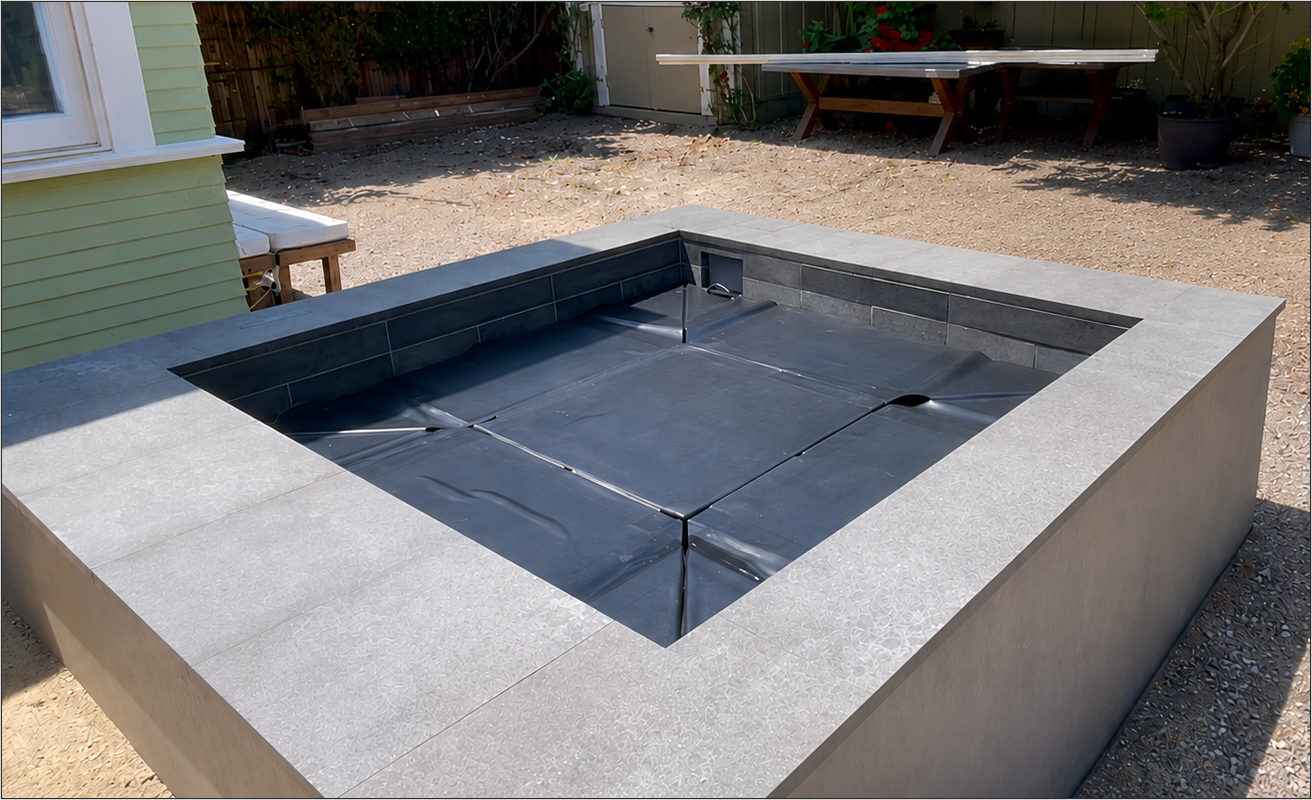
\includegraphics[
        width=5.55in,
        height=2.78in,
        keepaspectratio
    ]{deployed_functional_prototype}
};

\draw[DeepGreen,line width=0.8pt,rounded corners=7pt]
    ($(current page.north west)+(5.16in,-1.61in)$)
    rectangle
    ($(current page.north east)+(-0.42in,-4.47in)$);

\node[
    anchor=north west,
    text=Muted,
    font=\sffamily\fontsize{6.2}{6.9}\selectfont
]
at ($(current page.north west)+(5.18in,-4.54in)$)
{Functional foam model deployed over the sponsor's in-ground spa.};

% Image-strip title
\node[
    anchor=north west,
    text=DeepGreen,
    font=\sffamily\bfseries\fontsize{8.1}{8.8}\selectfont
]
at ($(current page.north west)+(0.43in,-4.78in)$)
{PRODUCT DEVELOPMENT AND FINAL ARCHITECTURE};

% Five-image development strip — CAD-first sequence
% Image 1: topside CAD
\node[anchor=center,inner sep=0pt]
at ($(current page.north west)+(1.47in,-5.73in)$)
{
    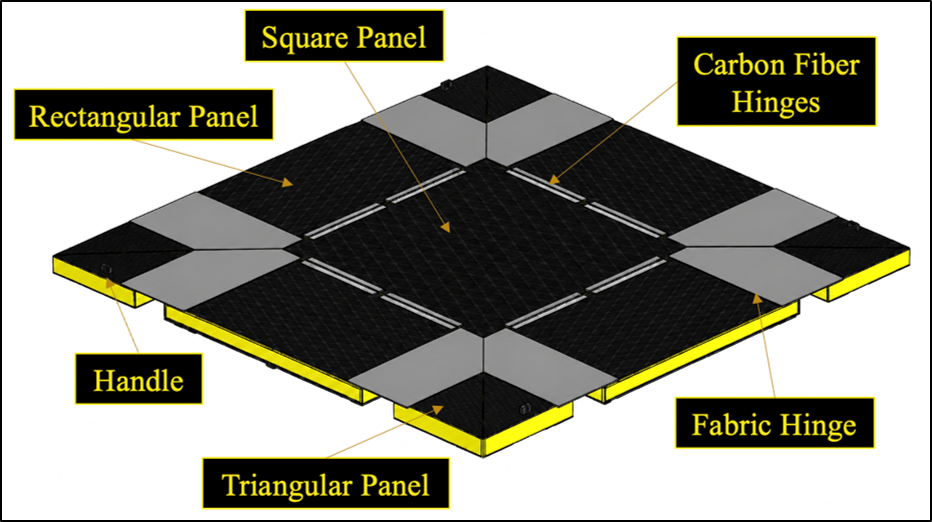
\includegraphics[
        width=1.92in,
        height=1.30in,
        keepaspectratio
    ]{Toro_Cover_topside_Cad}
};
\draw[RuleGray,line width=0.55pt,rounded corners=4pt]
    ($(current page.north west)+(0.43in,-5.04in)$)
    rectangle
    ($(current page.north west)+(2.51in,-6.43in)$);

% Image 2: underside CAD
\node[anchor=center,inner sep=0pt]
at ($(current page.north west)+(3.66in,-5.73in)$)
{
    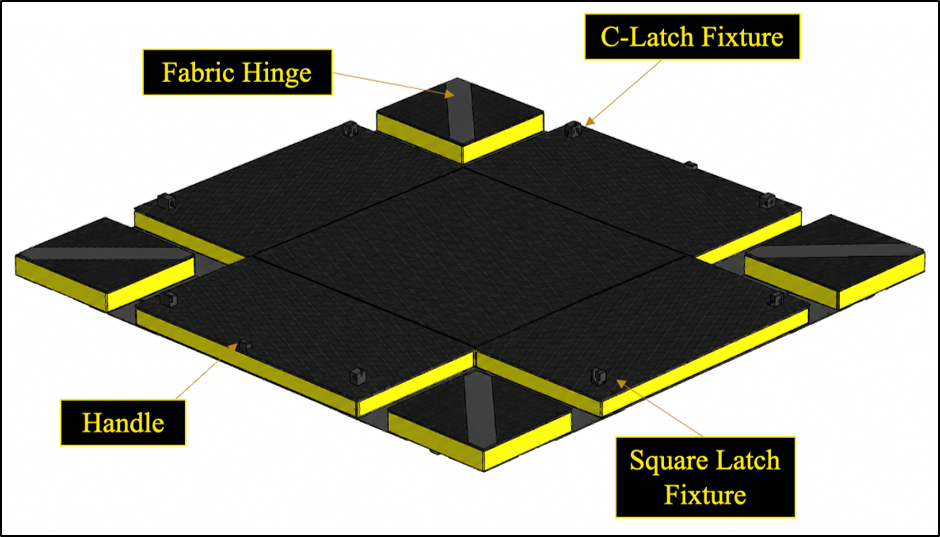
\includegraphics[
        width=1.92in,
        height=1.30in,
        keepaspectratio
    ]{toro_cover_underside_cad}
};
\draw[RuleGray,line width=0.55pt,rounded corners=4pt]
    ($(current page.north west)+(2.62in,-5.04in)$)
    rectangle
    ($(current page.north west)+(4.70in,-6.43in)$);

% Image 3: folded CAD
\node[anchor=center,inner sep=0pt]
at ($(current page.north west)+(5.85in,-5.73in)$)
{
    \includegraphics[
        width=1.92in,
        height=1.30in,
        keepaspectratio
    ]{\detokenize{Toro_Cover_folded Configuration}}
};
\draw[RuleGray,line width=0.55pt,rounded corners=4pt]
    ($(current page.north west)+(4.81in,-5.04in)$)
    rectangle
    ($(current page.north west)+(6.89in,-6.43in)$);

% Image 4: dual-use product concept
\node[anchor=center,inner sep=0pt]
at ($(current page.north west)+(8.04in,-5.73in)$)
{
    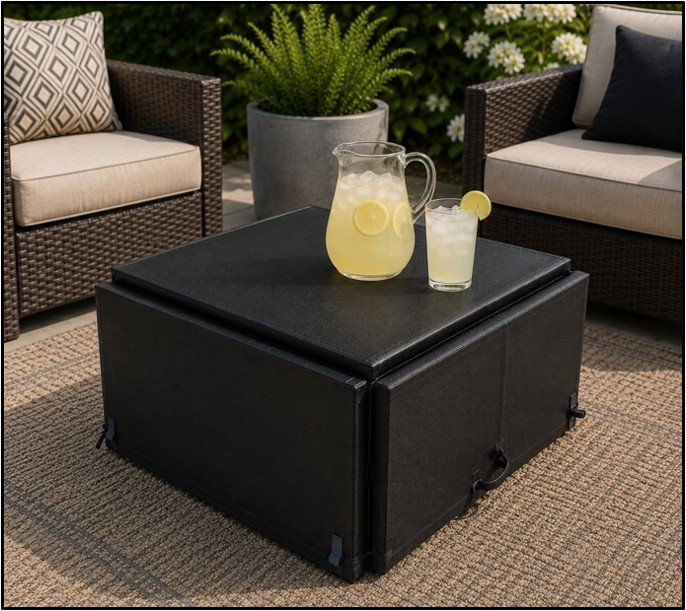
\includegraphics[
        width=1.92in,
        height=1.30in,
        keepaspectratio
    ]{generative_AI_concept_toro_cover_art}
};
\draw[RuleGray,line width=0.55pt,rounded corners=4pt]
    ($(current page.north west)+(7.00in,-5.04in)$)
    rectangle
    ($(current page.north west)+(9.08in,-6.43in)$);

% Image 5: folded foam functional prototype
% The portrait photograph is deliberately clipped to the landscape frame
% so the ottoman fills the card without extending beyond its border.
\begin{scope}
\clip[rounded corners=4pt]
    ($(current page.north west)+(9.19in,-5.04in)$)
    rectangle
    ($(current page.north east)+(-0.43in,-6.43in)$);

% Keep the original image proportions and center it within the existing card.
\node[anchor=center,inner sep=0pt]
at ($(current page.north west)+(9.88in,-5.735in)$)
{
    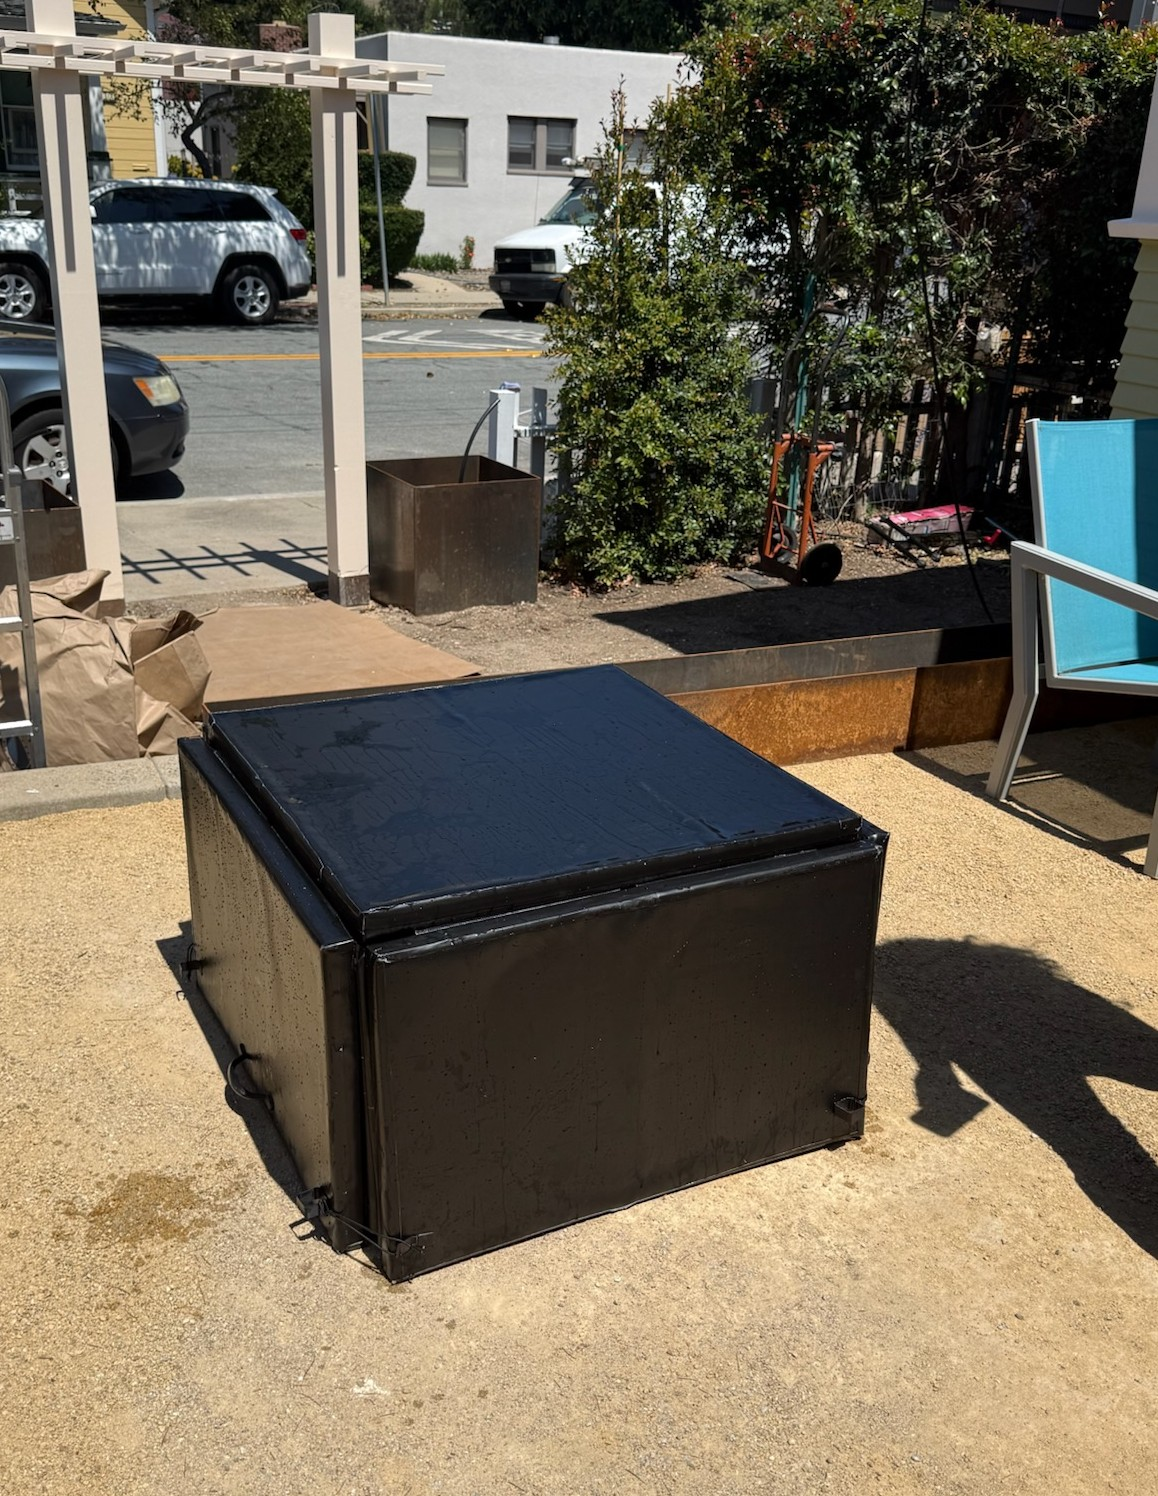
\includegraphics[
        width=1.58in,
        height=1.28in,
        keepaspectratio
    ]{foam_model_folded_backyard_image}
};
\end{scope}

\draw[RuleGray,line width=0.55pt,rounded corners=4pt]
    ($(current page.north west)+(9.19in,-5.04in)$)
    rectangle
    ($(current page.north east)+(-0.43in,-6.43in)$);

% Larger captions
\node[anchor=north,align=center,text width=1.95in,text=Muted,
      font=\sffamily\fontsize{6.8}{7.4}\selectfont]
at ($(current page.north west)+(1.47in,-6.49in)$)
{Topside panel architecture};

\node[anchor=north,align=center,text width=1.95in,text=Muted,
      font=\sffamily\fontsize{6.8}{7.4}\selectfont]
at ($(current page.north west)+(3.66in,-6.49in)$)
{Underside hinge architecture};

\node[anchor=north,align=center,text width=1.95in,text=Muted,
      font=\sffamily\fontsize{6.8}{7.4}\selectfont]
at ($(current page.north west)+(5.85in,-6.49in)$)
{Folded CAD configuration};

\node[anchor=north,align=center,text width=1.95in,text=Muted,
      font=\sffamily\fontsize{6.8}{7.4}\selectfont]
at ($(current page.north west)+(8.04in,-6.49in)$)
{Dual-use product vision};

\node[anchor=north,align=center,text width=1.95in,text=Muted,
      font=\sffamily\fontsize{6.8}{7.4}\selectfont]
at ($(current page.north west)+(9.88in,-6.49in)$)
{Folded foam prototype};

% Page 1 resource bar — centered and non-repeated resources
\fill[Panel,rounded corners=4pt]
    ($(current page.north west)+(0.43in,-7.05in)$)
    rectangle
    ($(current page.north east)+(-0.43in,-7.64in)$);
\draw[RuleGray,line width=0.5pt,rounded corners=4pt]
    ($(current page.north west)+(0.43in,-7.05in)$)
    rectangle
    ($(current page.north east)+(-0.43in,-7.64in)$);

\node[
    anchor=center,
    align=center,
    text=DeepGreen,
    font=\sffamily\bfseries\fontsize{6.9}{7.5}\selectfont
]
at ($(current page.north)+(0,-7.345in)$)
{\href{\ToroDrawingLink}{\faDraftingCompass\ DRAWING PACKAGE}
\hspace{24pt}
\href{\ToroDimensionsLink}{\faImage\ DIMENSION STUDY}
\hspace{24pt}
\href{\ToroProblemLink}{\faFileImage\ PROBLEM STATEMENT}};

% Footer
\node[
    anchor=south west,
    text=white,
    font=\sffamily\bfseries\fontsize{7.1}{7.7}\selectfont
]
at ($(current page.south west)+(0.42in,0.17in)$)
{\hyperlink{composites}{\faArrowLeft\ COMPOSITES}};

\node[
    anchor=south,
    text=white,
    font=\sffamily\fontsize{7.0}{7.6}\selectfont
]
at ($(current page.south)+(0,0.17in)$)
{TORO COVER \hspace{6pt} 1 / 3};

\node[
    anchor=south east,
    text=white,
    font=\sffamily\bfseries\fontsize{7.1}{7.7}\selectfont
]
at ($(current page.south east)+(-0.42in,0.17in)$)
{MANUFACTURING-DRIVEN DESIGN \faArrowRight};

\end{tikzpicture}


% ============================================================
% PAGE 2 — MANUFACTURING-DRIVEN DESIGN
% ============================================================

\clearpage
\thispagestyle{empty}
\hypertarget{toro-manufacturing}{}
\null

\begin{tikzpicture}[remember picture,overlay]

% Background and bars
\fill[white]
    (current page.south west)
    rectangle
    (current page.north east);

\fill[DeepGreen]
    (current page.north west)
    rectangle
    ($(current page.north east)+(0,-0.095in)$);

\fill[PolyGold]
    ($(current page.north west)+(0,-0.095in)$)
    rectangle
    ($(current page.north east)+(0,-0.14in)$);

\fill[DeepGreen]
    (current page.south west)
    rectangle
    ($(current page.south east)+(0,0.36in)$);

\fill[PolyGold]
    ($(current page.south west)+(0,0.36in)$)
    rectangle
    ($(current page.south east)+(0,0.405in)$);

% Header
\node[
    anchor=north west,
    text=PolyGold,
    font=\sffamily\bfseries\fontsize{8.1}{8.7}\selectfont
]
at ($(current page.north west)+(0.42in,-0.39in)$)
{TORO COVER \hspace{5pt}/\hspace{5pt} DESIGN FOR MANUFACTURABILITY};

\node[
    anchor=north west,
    text=DeepGreen,
    font=\bfseries\fontsize{23}{24}\selectfont
]
at ($(current page.north west)+(0.40in,-0.67in)$)
{THE ENVELOPE METHOD};

\node[
    anchor=north west,
    text=Muted,
    font=\sffamily\fontsize{8.7}{9.6}\selectfont
]
at ($(current page.north west)+(0.42in,-1.12in)$)
{A one-layup process developed for unusually thick insulated composite sandwich panels};

\fill[PolyGold]
    ($(current page.north west)+(0.42in,-1.36in)$)
    rectangle
    ($(current page.north west)+(5.30in,-1.315in)$);

% Process explanation
\fill[SoftGold,rounded corners=5pt]
    ($(current page.north west)+(0.42in,-1.61in)$)
    rectangle
    ($(current page.north east)+(-0.42in,-2.90in)$);

\fill[PolyGold]
    ($(current page.north west)+(0.42in,-1.61in)$)
    rectangle
    ($(current page.north west)+(0.52in,-2.90in)$);

\node[
    anchor=north west,
    text=DeepGreen,
    font=\sffamily\bfseries\fontsize{7.9}{8.6}\selectfont
]
at ($(current page.north west)+(0.67in,-1.76in)$)
{PROCESS INNOVATION};

\node[
    anchor=north west,
    align=left,
    text width=9.55in,
    text=Ink,
    font=\fontsize{7.35}{8.75}\selectfont
]
at ($(current page.north west)+(0.67in,-2.02in)$)
{
Weight reduction and insulation were both essential, leading to the selection of an
XPS foam core. Because XPS could not tolerate composite heat-cure temperatures, prepreg
processing was not practical and the panels had to be manufactured by wet layup with a
room-temperature cure. To simplify this process, I waterjet-cut XPS perimeter strips from
excess foam and placed them around each core inside the vacuum enclosure. Under vacuum,
the top and bottom carbon skins met along the panel sides and compressed against this
border, eliminating a separate edge-banding layup and reducing corner pleating.
};

% Workflow title
\node[
    anchor=north west,
    text=DeepGreen,
    font=\sffamily\bfseries\fontsize{8.0}{8.7}\selectfont
]
at ($(current page.north west)+(0.43in,-3.06in)$)
{MANUFACTURING WORKFLOW};

% Row 1 image 1
\node[anchor=center,inner sep=0pt]
at ($(current page.north west)+(2.07in,-4.105in)$)
{
    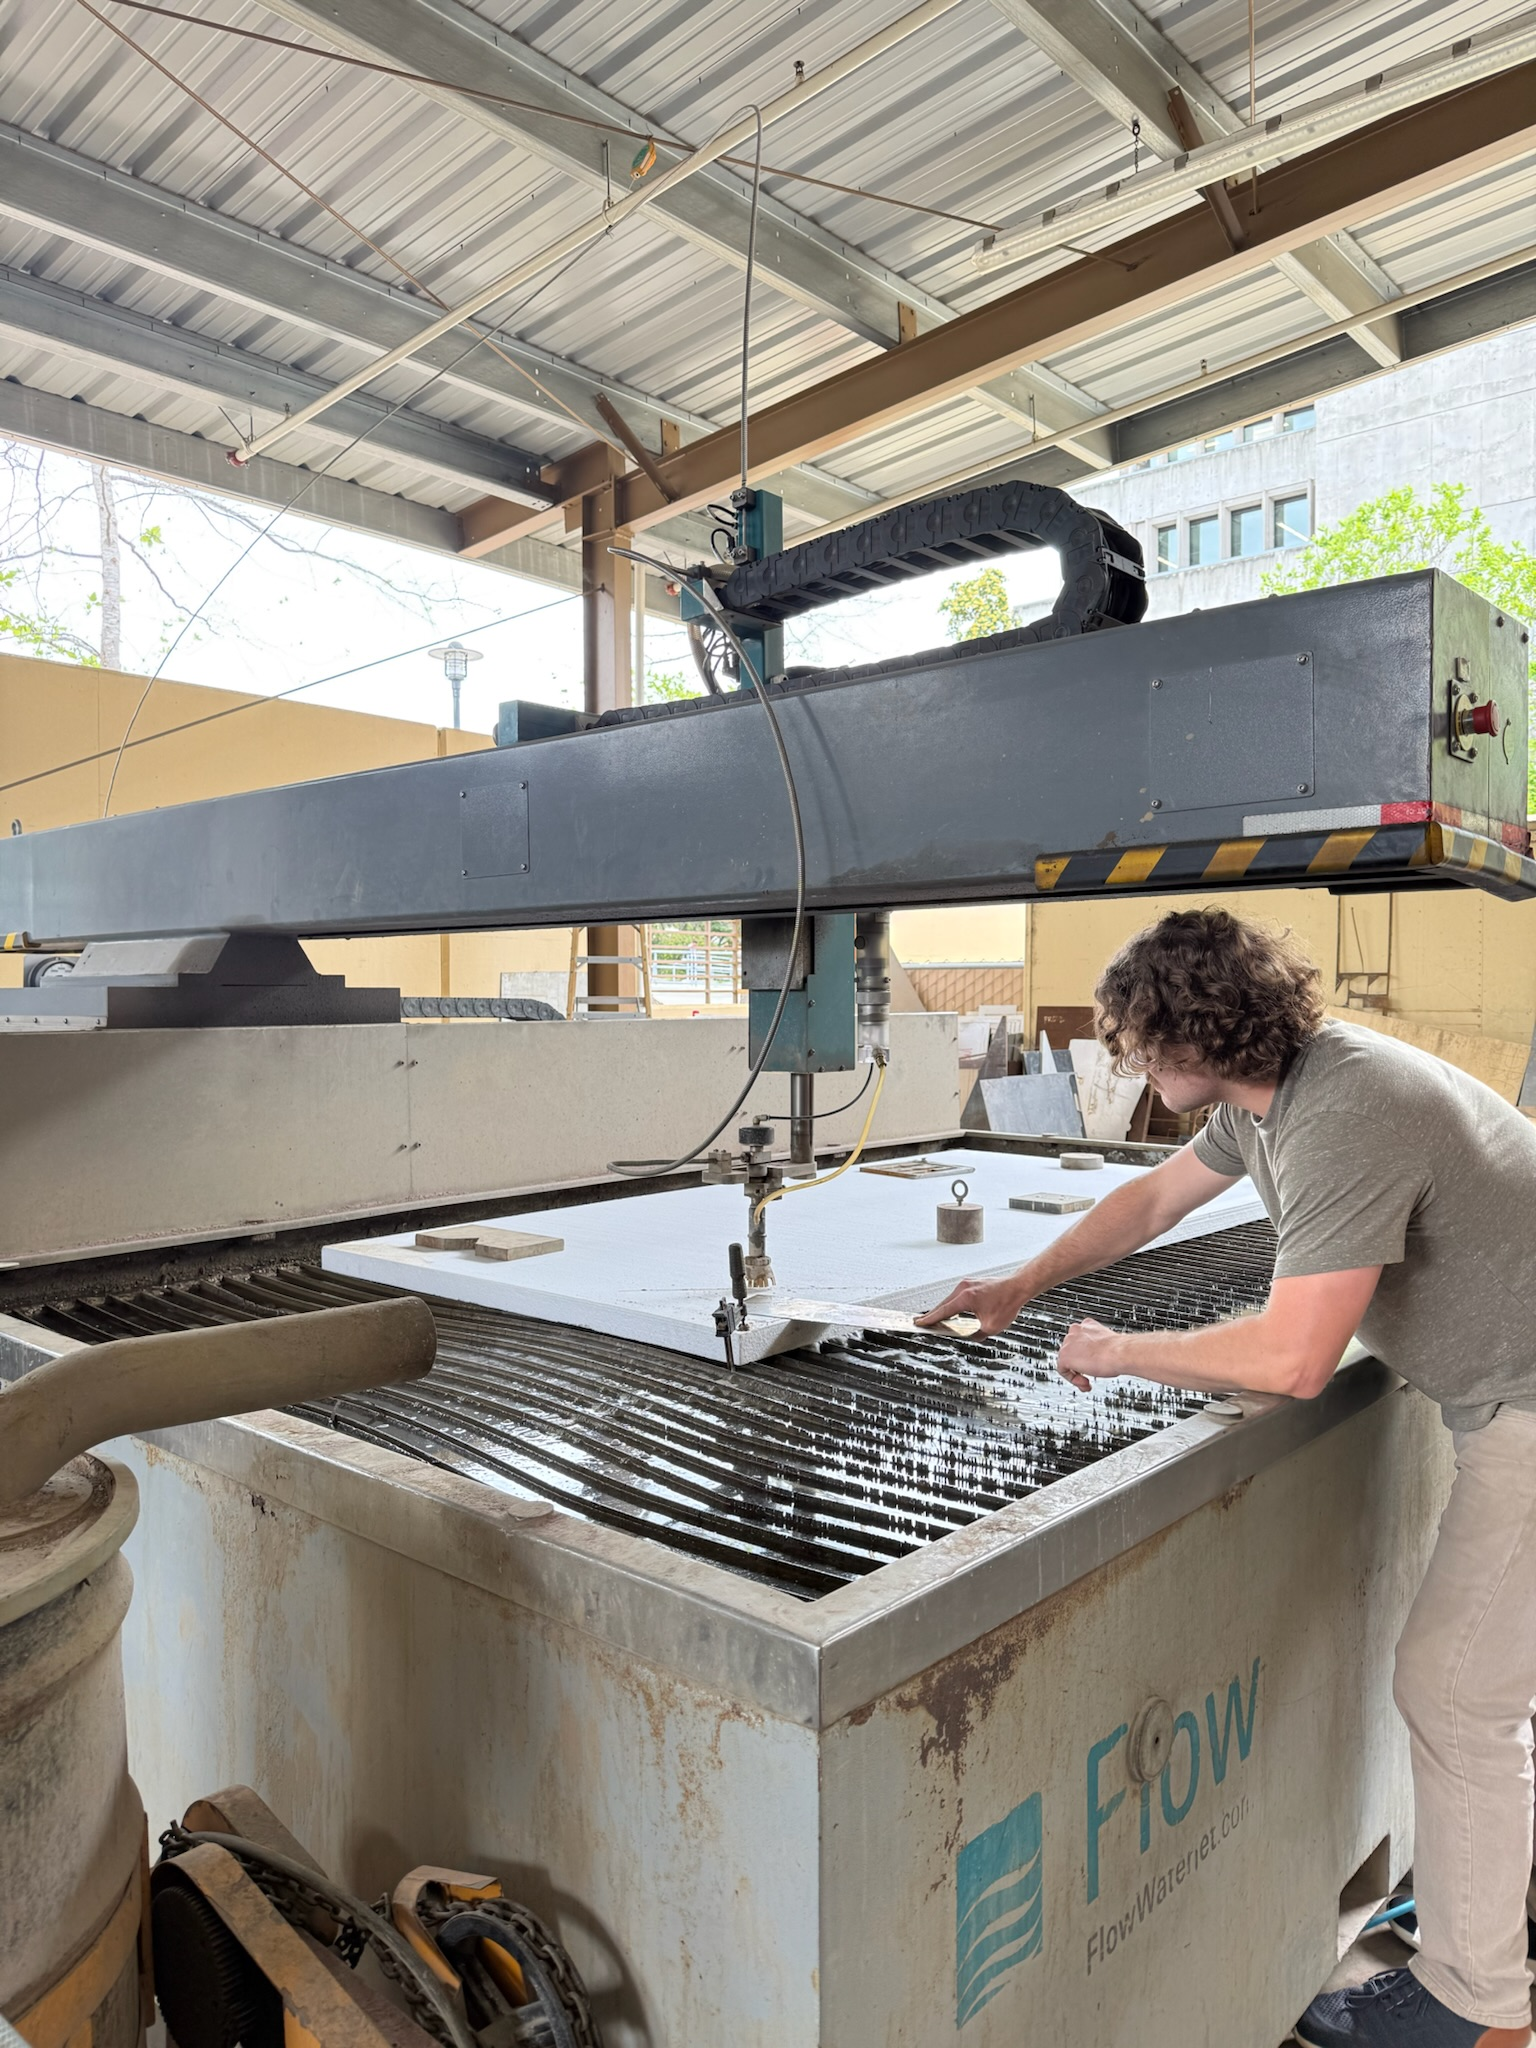
\includegraphics[
        width=3.10in,
        height=1.40in,
        keepaspectratio
    ]{waterjet_foam}
};
\draw[RuleGray,line width=0.55pt,rounded corners=4pt]
    ($(current page.north west)+(0.43in,-3.36in)$)
    rectangle
    ($(current page.north west)+(3.71in,-4.85in)$);

% Row 1 image 2
\node[anchor=center,inner sep=0pt]
at ($(current page.north west)+(5.50in,-4.105in)$)
{
    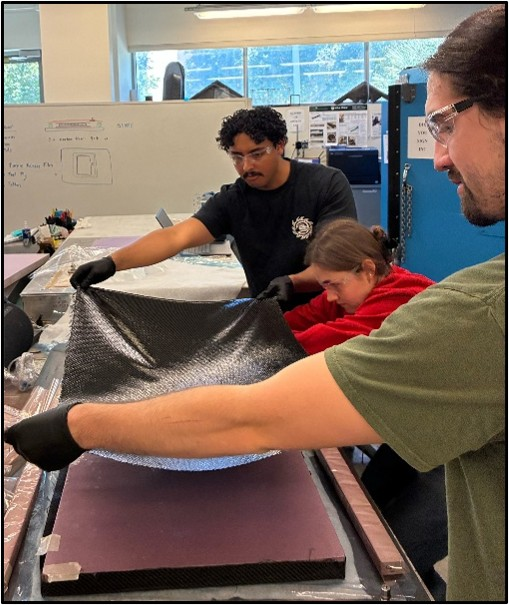
\includegraphics[
        width=3.10in,
        height=1.40in,
        keepaspectratio
    ]{group_layup}
};
\draw[RuleGray,line width=0.55pt,rounded corners=4pt]
    ($(current page.north west)+(3.86in,-3.36in)$)
    rectangle
    ($(current page.north west)+(7.14in,-4.85in)$);

% Row 1 image 3
\node[anchor=center,inner sep=0pt]
at ($(current page.north west)+(8.935in,-4.105in)$)
{
    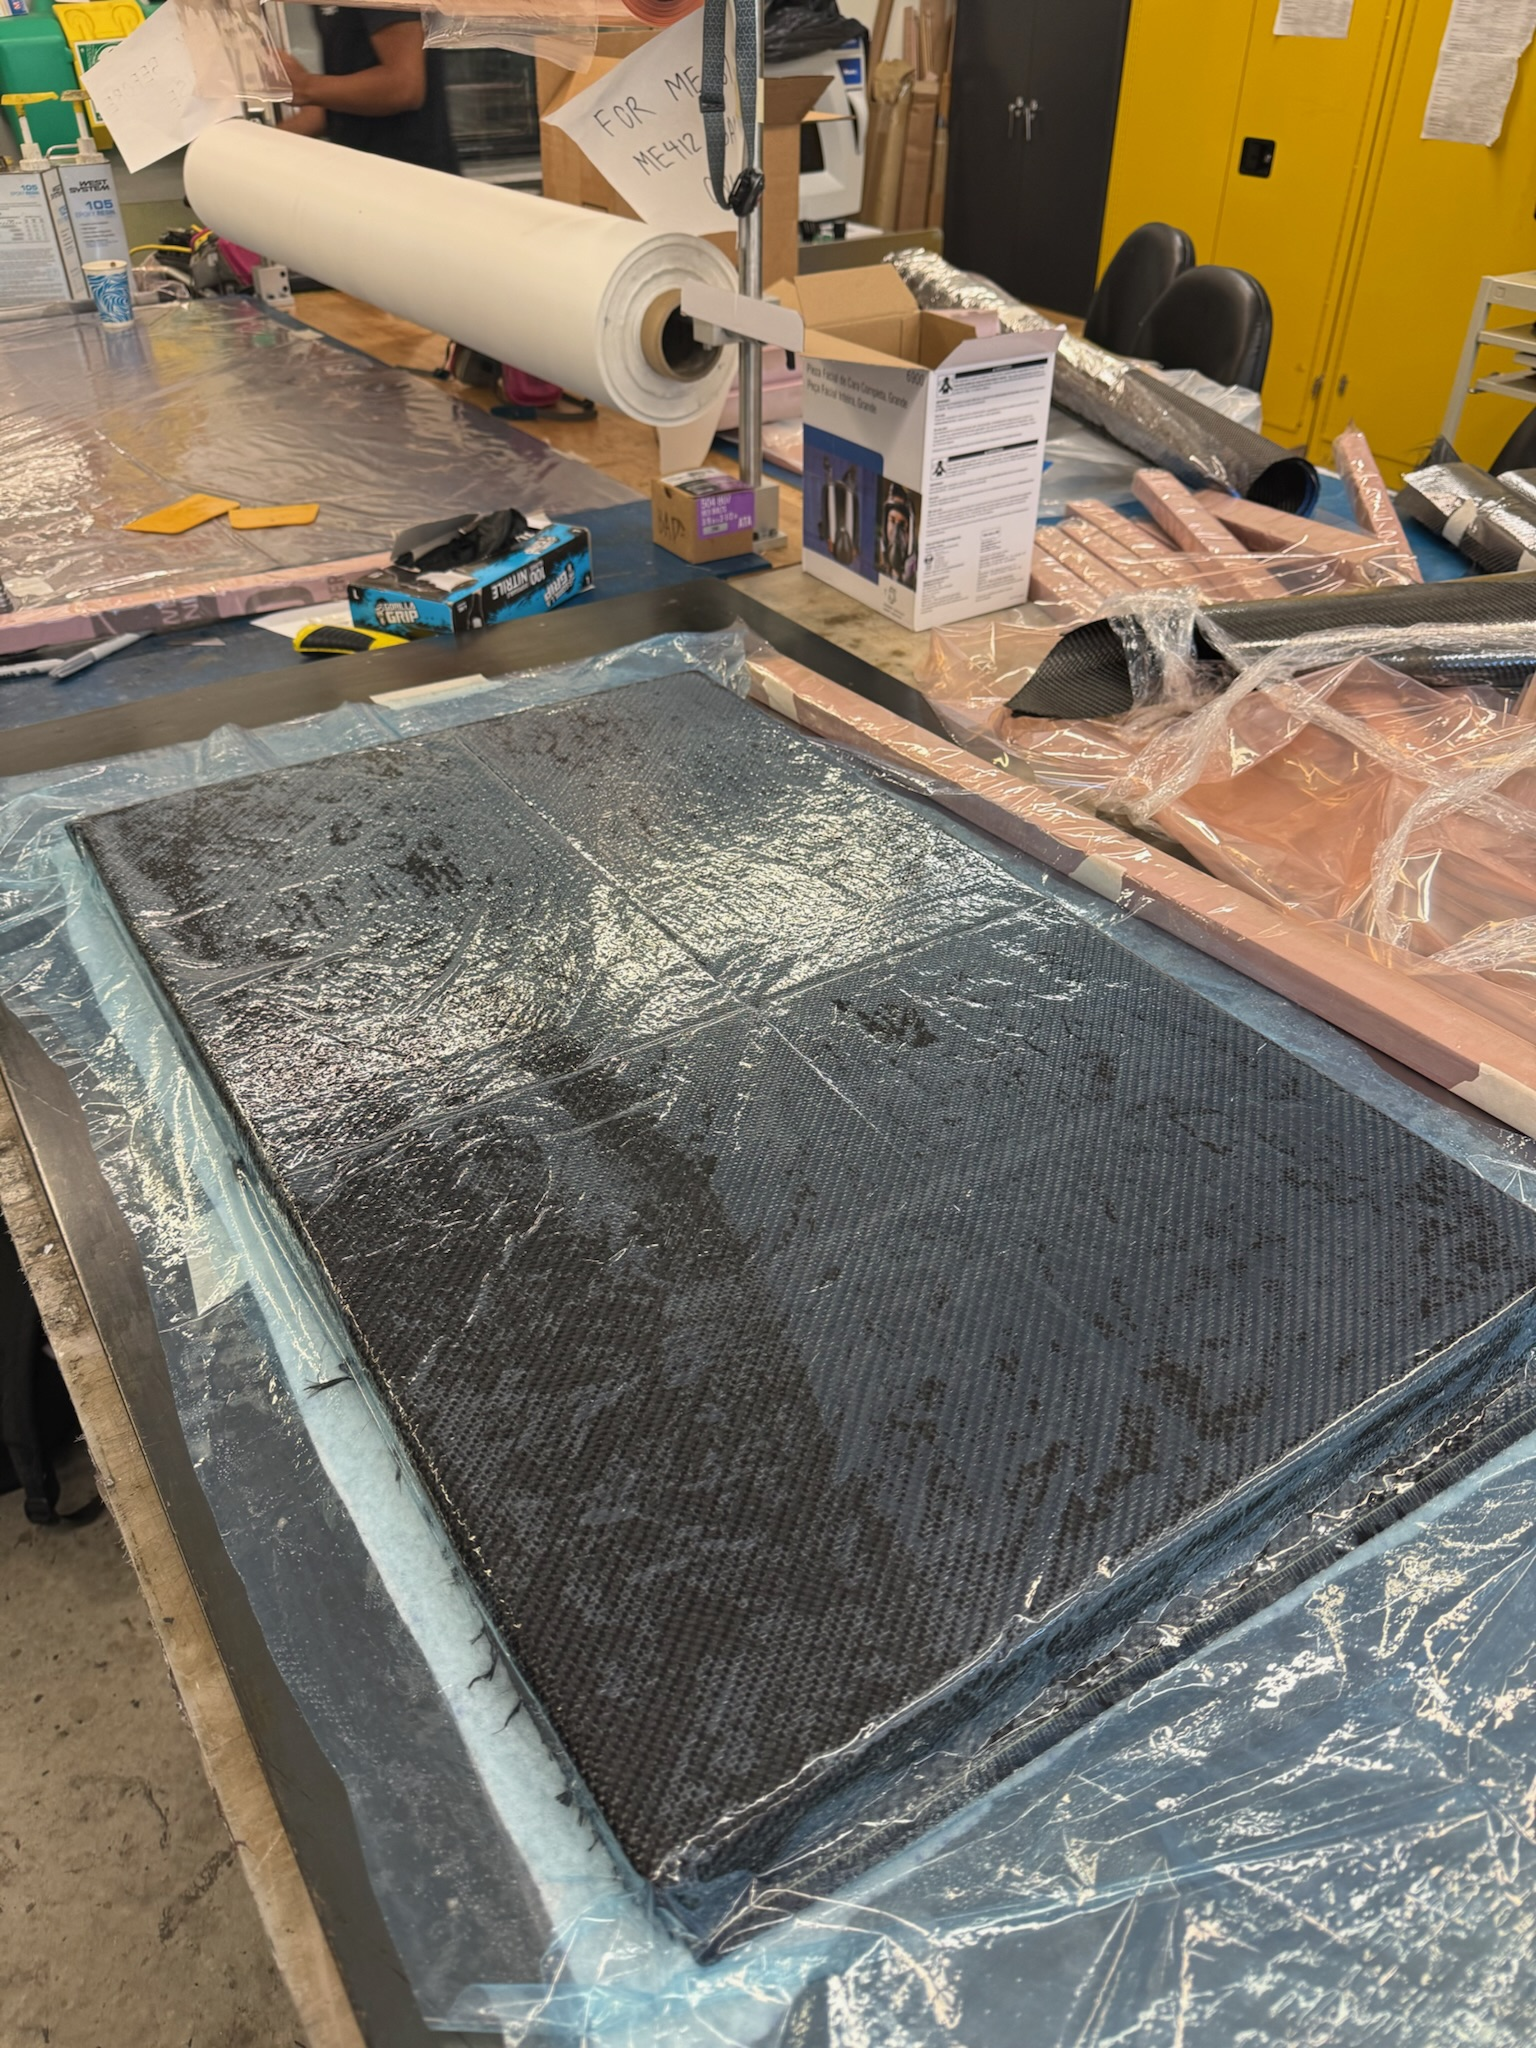
\includegraphics[
        width=3.10in,
        height=1.40in,
        keepaspectratio
    ]{blue_perforrated_film_layup}
};
\draw[RuleGray,line width=0.55pt,rounded corners=4pt]
    ($(current page.north west)+(7.29in,-3.36in)$)
    rectangle
    ($(current page.north east)+(-0.42in,-4.85in)$);

% Row 1 captions
\node[anchor=north,text=Muted,font=\sffamily\fontsize{6.7}{7.3}\selectfont]
at ($(current page.north west)+(2.07in,-4.90in)$)
{1. Waterjet-cut core and perimeter geometry};

\node[anchor=north,text=Muted,font=\sffamily\fontsize{6.7}{7.3}\selectfont]
at ($(current page.north west)+(5.50in,-4.90in)$)
{2. Team wet layup under my process guidance};

\node[anchor=north,text=Muted,font=\sffamily\fontsize{6.7}{7.3}\selectfont]
at ($(current page.north west)+(8.935in,-4.90in)$)
{3. Perforated film, breather, and vacuum enclosure};

% Row 2 image 1
\node[anchor=center,inner sep=0pt]
at ($(current page.north west)+(2.07in,-5.875in)$)
{
    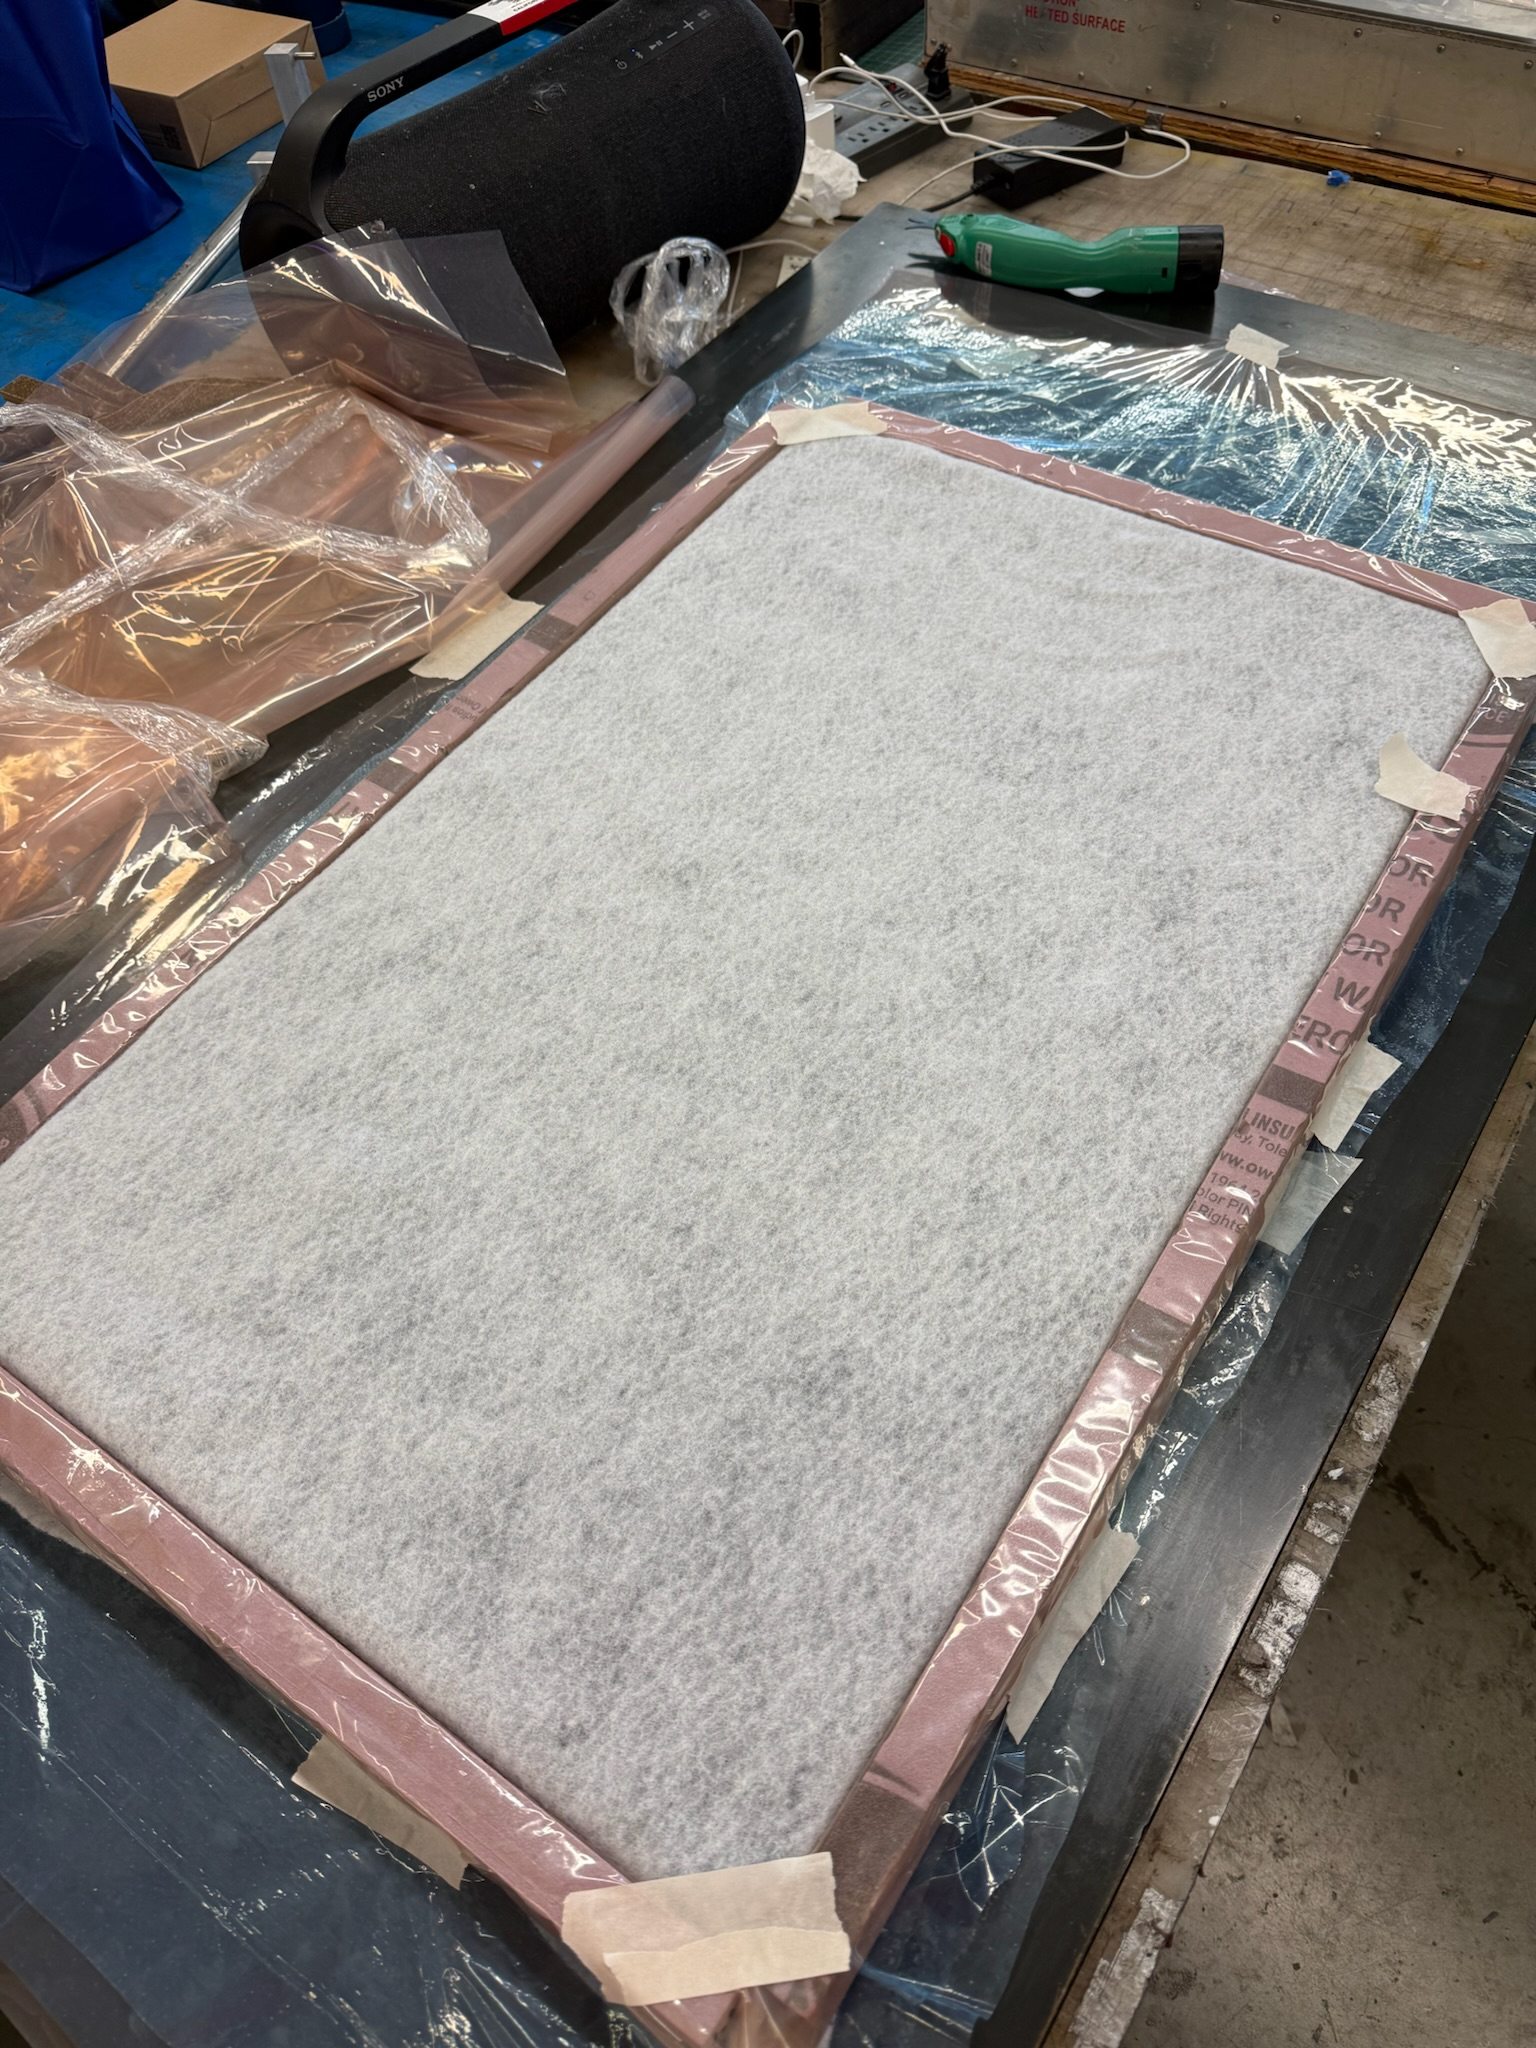
\includegraphics[
        width=3.10in,
        height=1.40in,
        keepaspectratio
    ]{completed_layup}
};
\draw[RuleGray,line width=0.55pt,rounded corners=4pt]
    ($(current page.north west)+(0.43in,-5.13in)$)
    rectangle
    ($(current page.north west)+(3.71in,-6.62in)$);

% Row 2 image 2 — oven chamber used only as a reliable vacuum enclosure; no heat applied
\node[anchor=center,inner sep=0pt]
at ($(current page.north west)+(5.50in,-5.875in)$)
{
    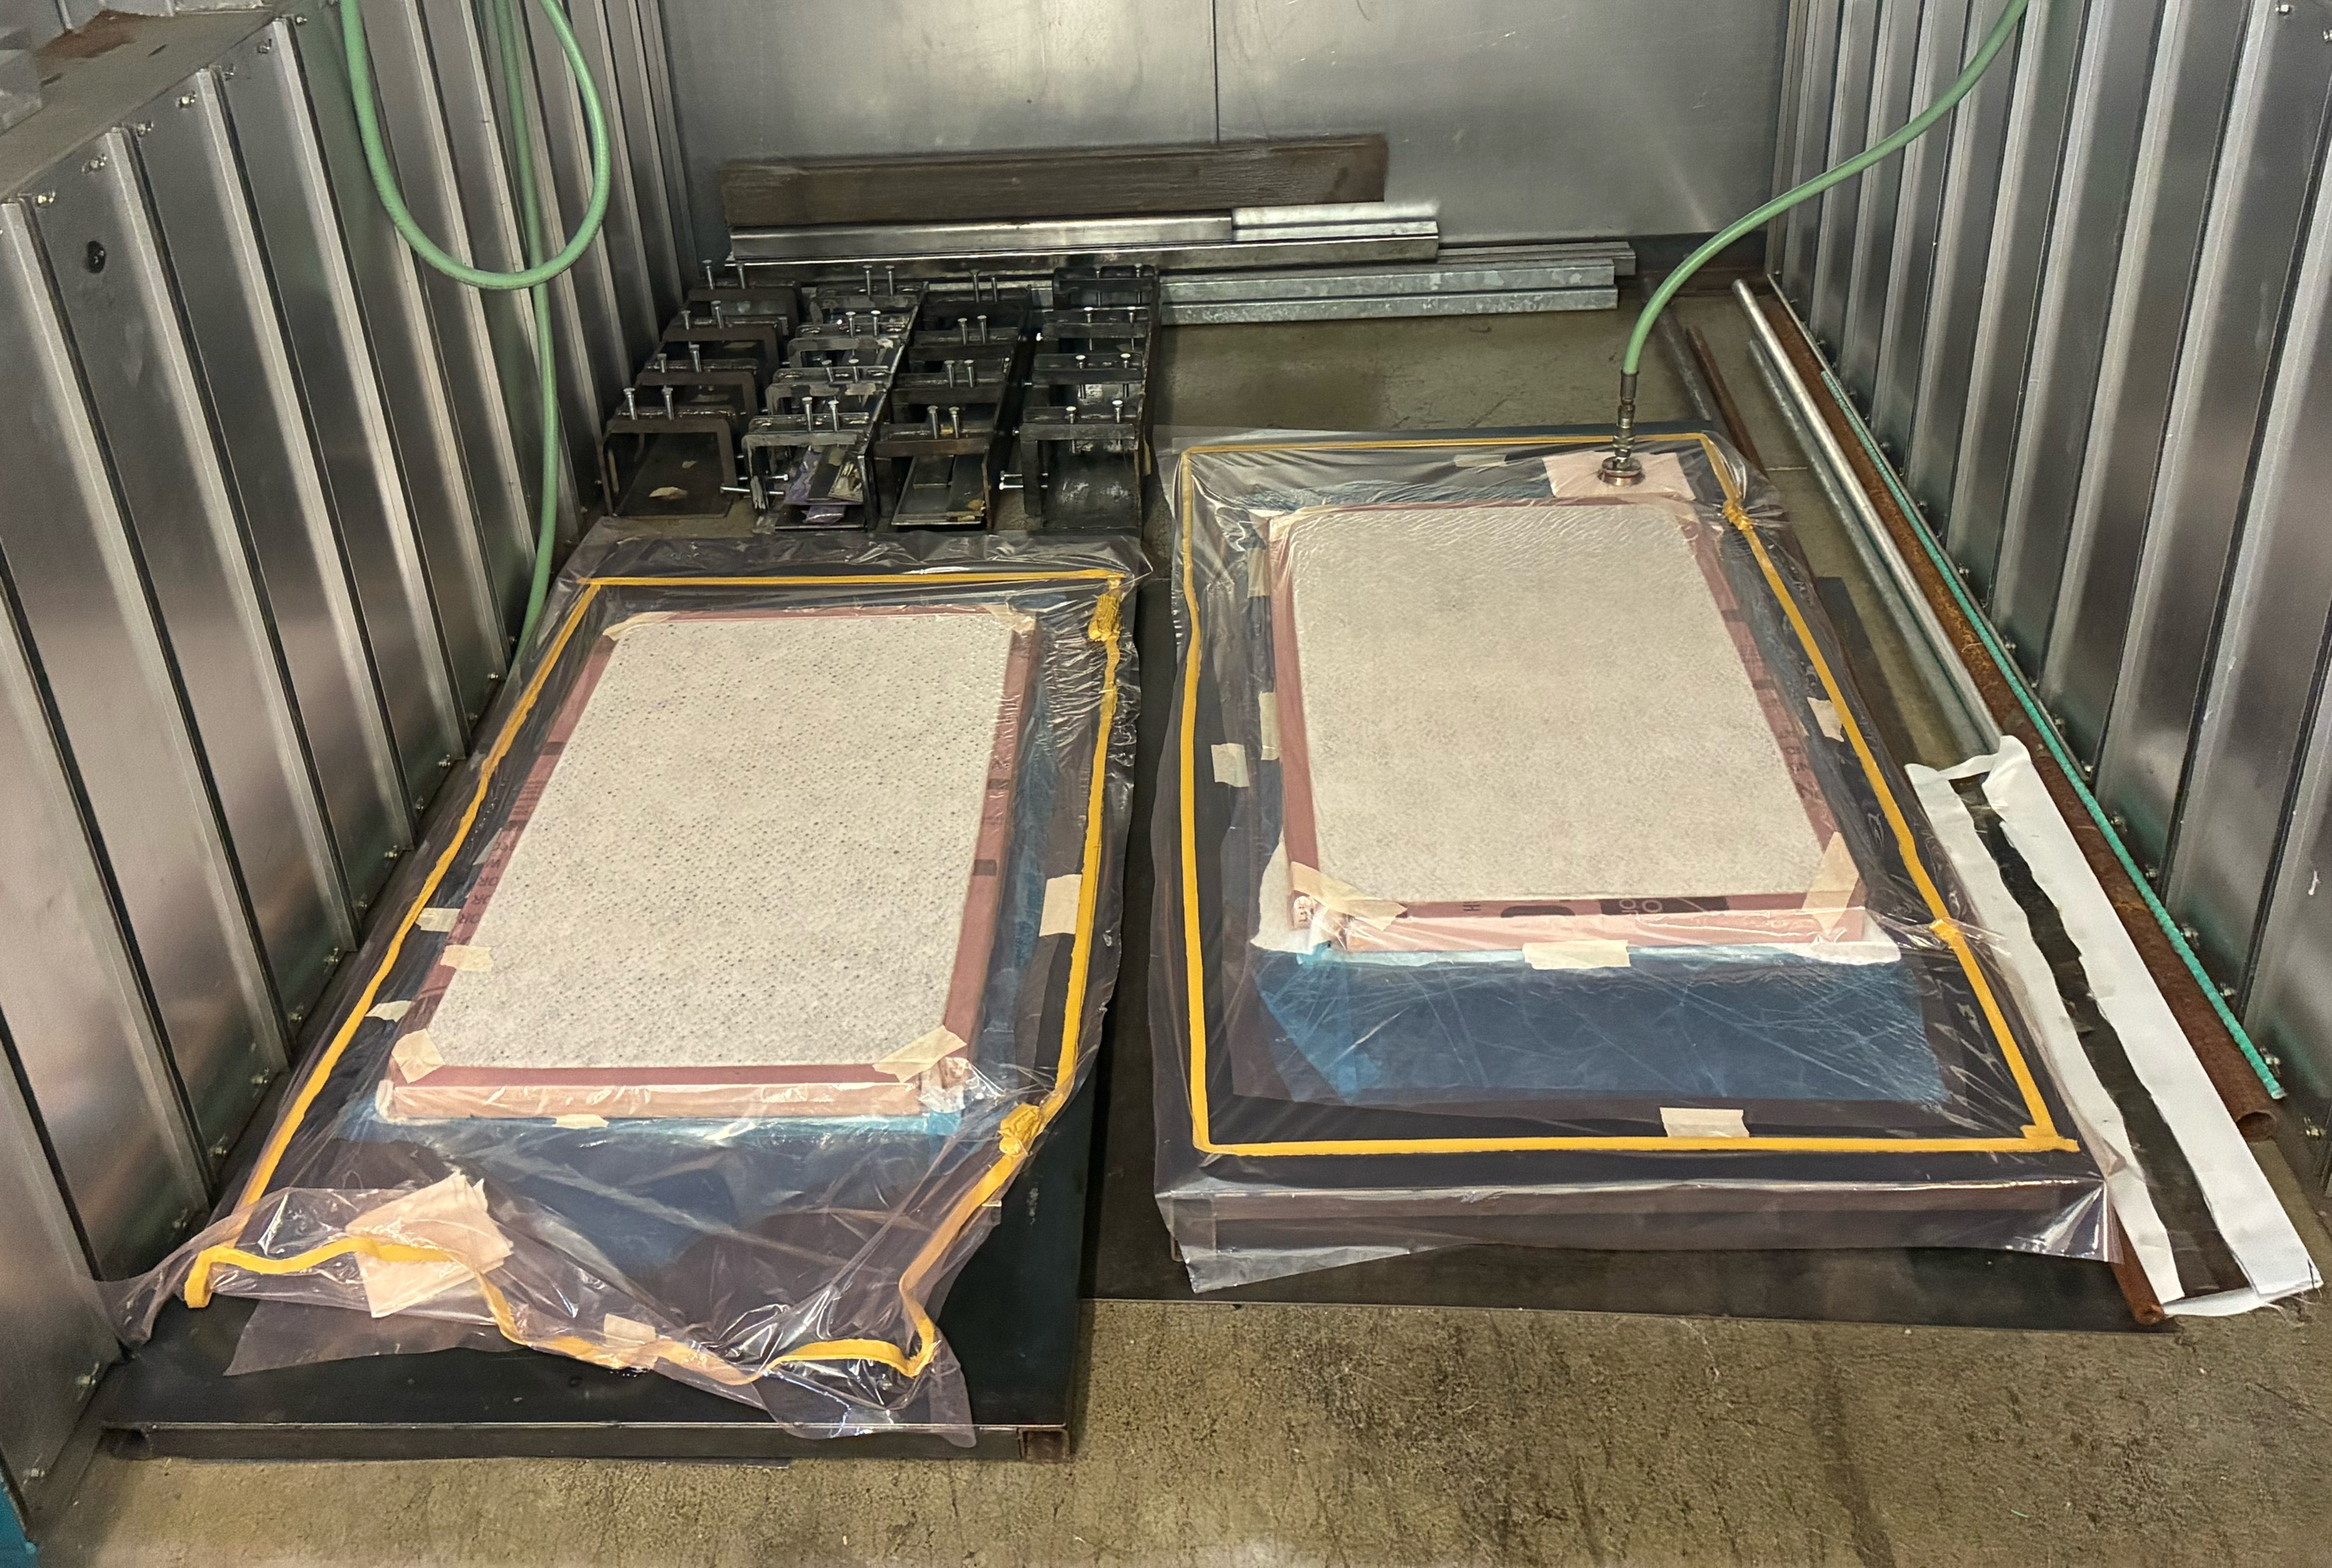
\includegraphics[
        width=3.10in,
        height=1.40in,
        keepaspectratio
    ]{layups_in_composite_oven_under_vacuumPressure}
};
\draw[RuleGray,line width=0.55pt,rounded corners=4pt]
    ($(current page.north west)+(3.86in,-5.13in)$)
    rectangle
    ($(current page.north west)+(7.14in,-6.62in)$);

% Row 2 image 3
\node[anchor=center,inner sep=0pt]
at ($(current page.north west)+(8.935in,-5.875in)$)
{
    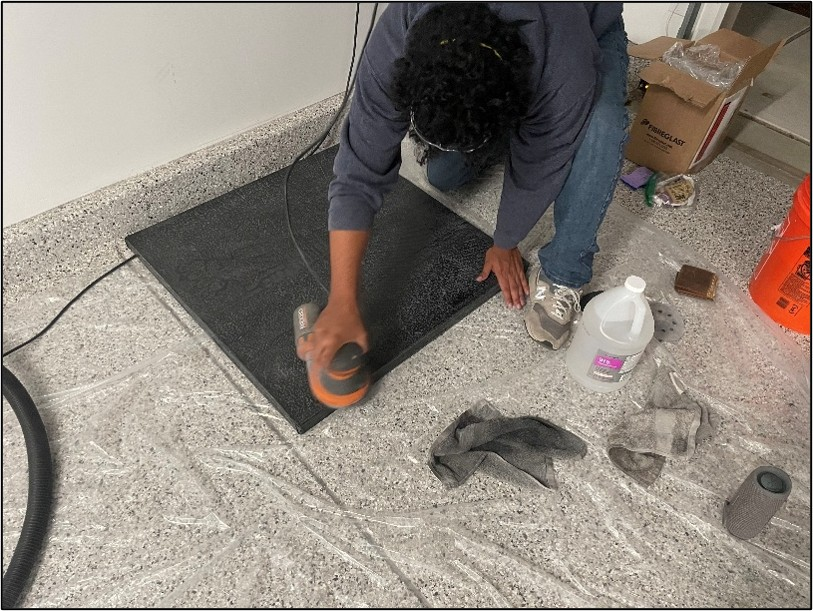
\includegraphics[
        width=3.10in,
        height=1.40in,
        keepaspectratio
    ]{garage_sanding}
};
\draw[RuleGray,line width=0.55pt,rounded corners=4pt]
    ($(current page.north west)+(7.29in,-5.13in)$)
    rectangle
    ($(current page.north east)+(-0.42in,-6.62in)$);

% Row 2 captions
\node[anchor=north,text=Muted,font=\sffamily\fontsize{6.7}{7.3}\selectfont]
at ($(current page.north west)+(2.07in,-6.67in)$)
{4. Fully saturated carbon skin and foam sandwich};

\node[anchor=north,text=Muted,font=\sffamily\fontsize{6.7}{7.3}\selectfont]
at ($(current page.north west)+(5.50in,-6.67in)$)
{5. Room-temperature cure under continuous vacuum};

\node[anchor=north,text=Muted,font=\sffamily\fontsize{6.7}{7.3}\selectfont]
at ($(current page.north west)+(8.935in,-6.67in)$)
{6. Post-processing and surface preparation};

% Bottom callouts
\fill[Panel,rounded corners=4pt]
    ($(current page.north west)+(0.43in,-6.95in)$)
    rectangle
    ($(current page.north west)+(5.48in,-7.60in)$);

\draw[RuleGray,line width=0.55pt,rounded corners=4pt]
    ($(current page.north west)+(0.43in,-6.95in)$)
    rectangle
    ($(current page.north west)+(5.48in,-7.60in)$);

\node[
    anchor=north west,
    text=DeepGreen,
    font=\sffamily\bfseries\fontsize{7.0}{7.6}\selectfont
]
at ($(current page.north west)+(0.63in,-7.08in)$)
{FROM THREE LAYUPS TO ONE};

\node[
    anchor=north west,
    align=left,
    text width=4.56in,
    text=Ink,
    font=\fontsize{6.45}{7.45}\selectfont
]
at ($(current page.north west)+(0.63in,-7.29in)$)
{
The Envelope Method reduced labor, cure cycles, handling,
alignment risk, and time spent forming numerous vacuum-bag
pleats around the 1.5-inch-thick XPS panels.
};

\fill[Panel,rounded corners=4pt]
    ($(current page.north west)+(5.68in,-6.95in)$)
    rectangle
    ($(current page.north east)+(-0.42in,-7.60in)$);

\draw[RuleGray,line width=0.55pt,rounded corners=4pt]
    ($(current page.north west)+(5.68in,-6.95in)$)
    rectangle
    ($(current page.north east)+(-0.42in,-7.60in)$);

\node[
    anchor=north west,
    text=DeepGreen,
    font=\sffamily\bfseries\fontsize{7.0}{7.6}\selectfont
]
at ($(current page.north west)+(5.88in,-7.08in)$)
{WHY SURFACE-BONDED HARDWARE};

\node[
    anchor=north west,
    align=left,
    text width=4.55in,
    text=Ink,
    font=\fontsize{6.45}{7.45}\selectfont
]
at ($(current page.north west)+(5.88in,-7.29in)$)
{
Adhesively bonded hinges and fixtures preserved the clean
composite exterior and avoided drilled inserts, foam-core
crushing, added stress concentrations, and new leak paths.
};


% Footer
\node[
    anchor=south west,
    text=white,
    font=\sffamily\bfseries\fontsize{7.1}{7.7}\selectfont
]
at ($(current page.south west)+(0.42in,0.17in)$)
{\faArrowLeft\ PRODUCT ARCHITECTURE};

\node[
    anchor=south,
    text=white,
    font=\sffamily\fontsize{7.0}{7.6}\selectfont
]
at ($(current page.south)+(0,0.17in)$)
{TORO COVER \hspace{6pt} 2 / 3};

\node[
    anchor=south east,
    text=white,
    font=\sffamily\bfseries\fontsize{7.1}{7.7}\selectfont
]
at ($(current page.south east)+(-0.42in,0.17in)$)
{VALIDATION \& TAKEAWAYS \faArrowRight};

\end{tikzpicture}


% ============================================================
% PAGE 3 — FINISHING, VALIDATION, AND TAKEAWAYS
% ============================================================

\clearpage
\thispagestyle{empty}
\hypertarget{toro-results}{}
\null

\begin{tikzpicture}[remember picture,overlay]

% Background and bars
\fill[white]
    (current page.south west)
    rectangle
    (current page.north east);

\fill[DeepGreen]
    (current page.north west)
    rectangle
    ($(current page.north east)+(0,-0.095in)$);

\fill[PolyGold]
    ($(current page.north west)+(0,-0.095in)$)
    rectangle
    ($(current page.north east)+(0,-0.14in)$);

\fill[DeepGreen]
    (current page.south west)
    rectangle
    ($(current page.south east)+(0,0.36in)$);

\fill[PolyGold]
    ($(current page.south west)+(0,0.36in)$)
    rectangle
    ($(current page.south east)+(0,0.405in)$);

% Header
\node[
    anchor=north west,
    text=PolyGold,
    font=\sffamily\bfseries\fontsize{8.1}{8.7}\selectfont
]
at ($(current page.north west)+(0.42in,-0.39in)$)
{TORO COVER \hspace{5pt}/\hspace{5pt} VALIDATION AND ENGINEERING TAKEAWAYS};

\node[
    anchor=north west,
    text=DeepGreen,
    font=\bfseries\fontsize{22.5}{23.5}\selectfont
]
at ($(current page.north west)+(0.40in,-0.67in)$)
{FROM PROTOTYPE TO PRODUCT PATHWAY};

\node[
    anchor=north west,
    text=Muted,
    font=\sffamily\fontsize{8.7}{9.6}\selectfont
]
at ($(current page.north west)+(0.42in,-1.12in)$)
{Environmental protection, usability testing, scope decisions, and lessons from technical leadership};

\fill[PolyGold]
    ($(current page.north west)+(0.42in,-1.36in)$)
    rectangle
    ($(current page.north west)+(5.8in,-1.315in)$);

% Finishing title
\node[
    anchor=north west,
    text=DeepGreen,
    font=\sffamily\bfseries\fontsize{8.0}{8.7}\selectfont
]
at ($(current page.north west)+(0.43in,-1.62in)$)
{OUTDOOR FINISHING AND ENVIRONMENTAL PROTECTION};

% Image 1
\node[anchor=center,inner sep=0pt]
at ($(current page.north west)+(1.705in,-2.655in)$)
{
    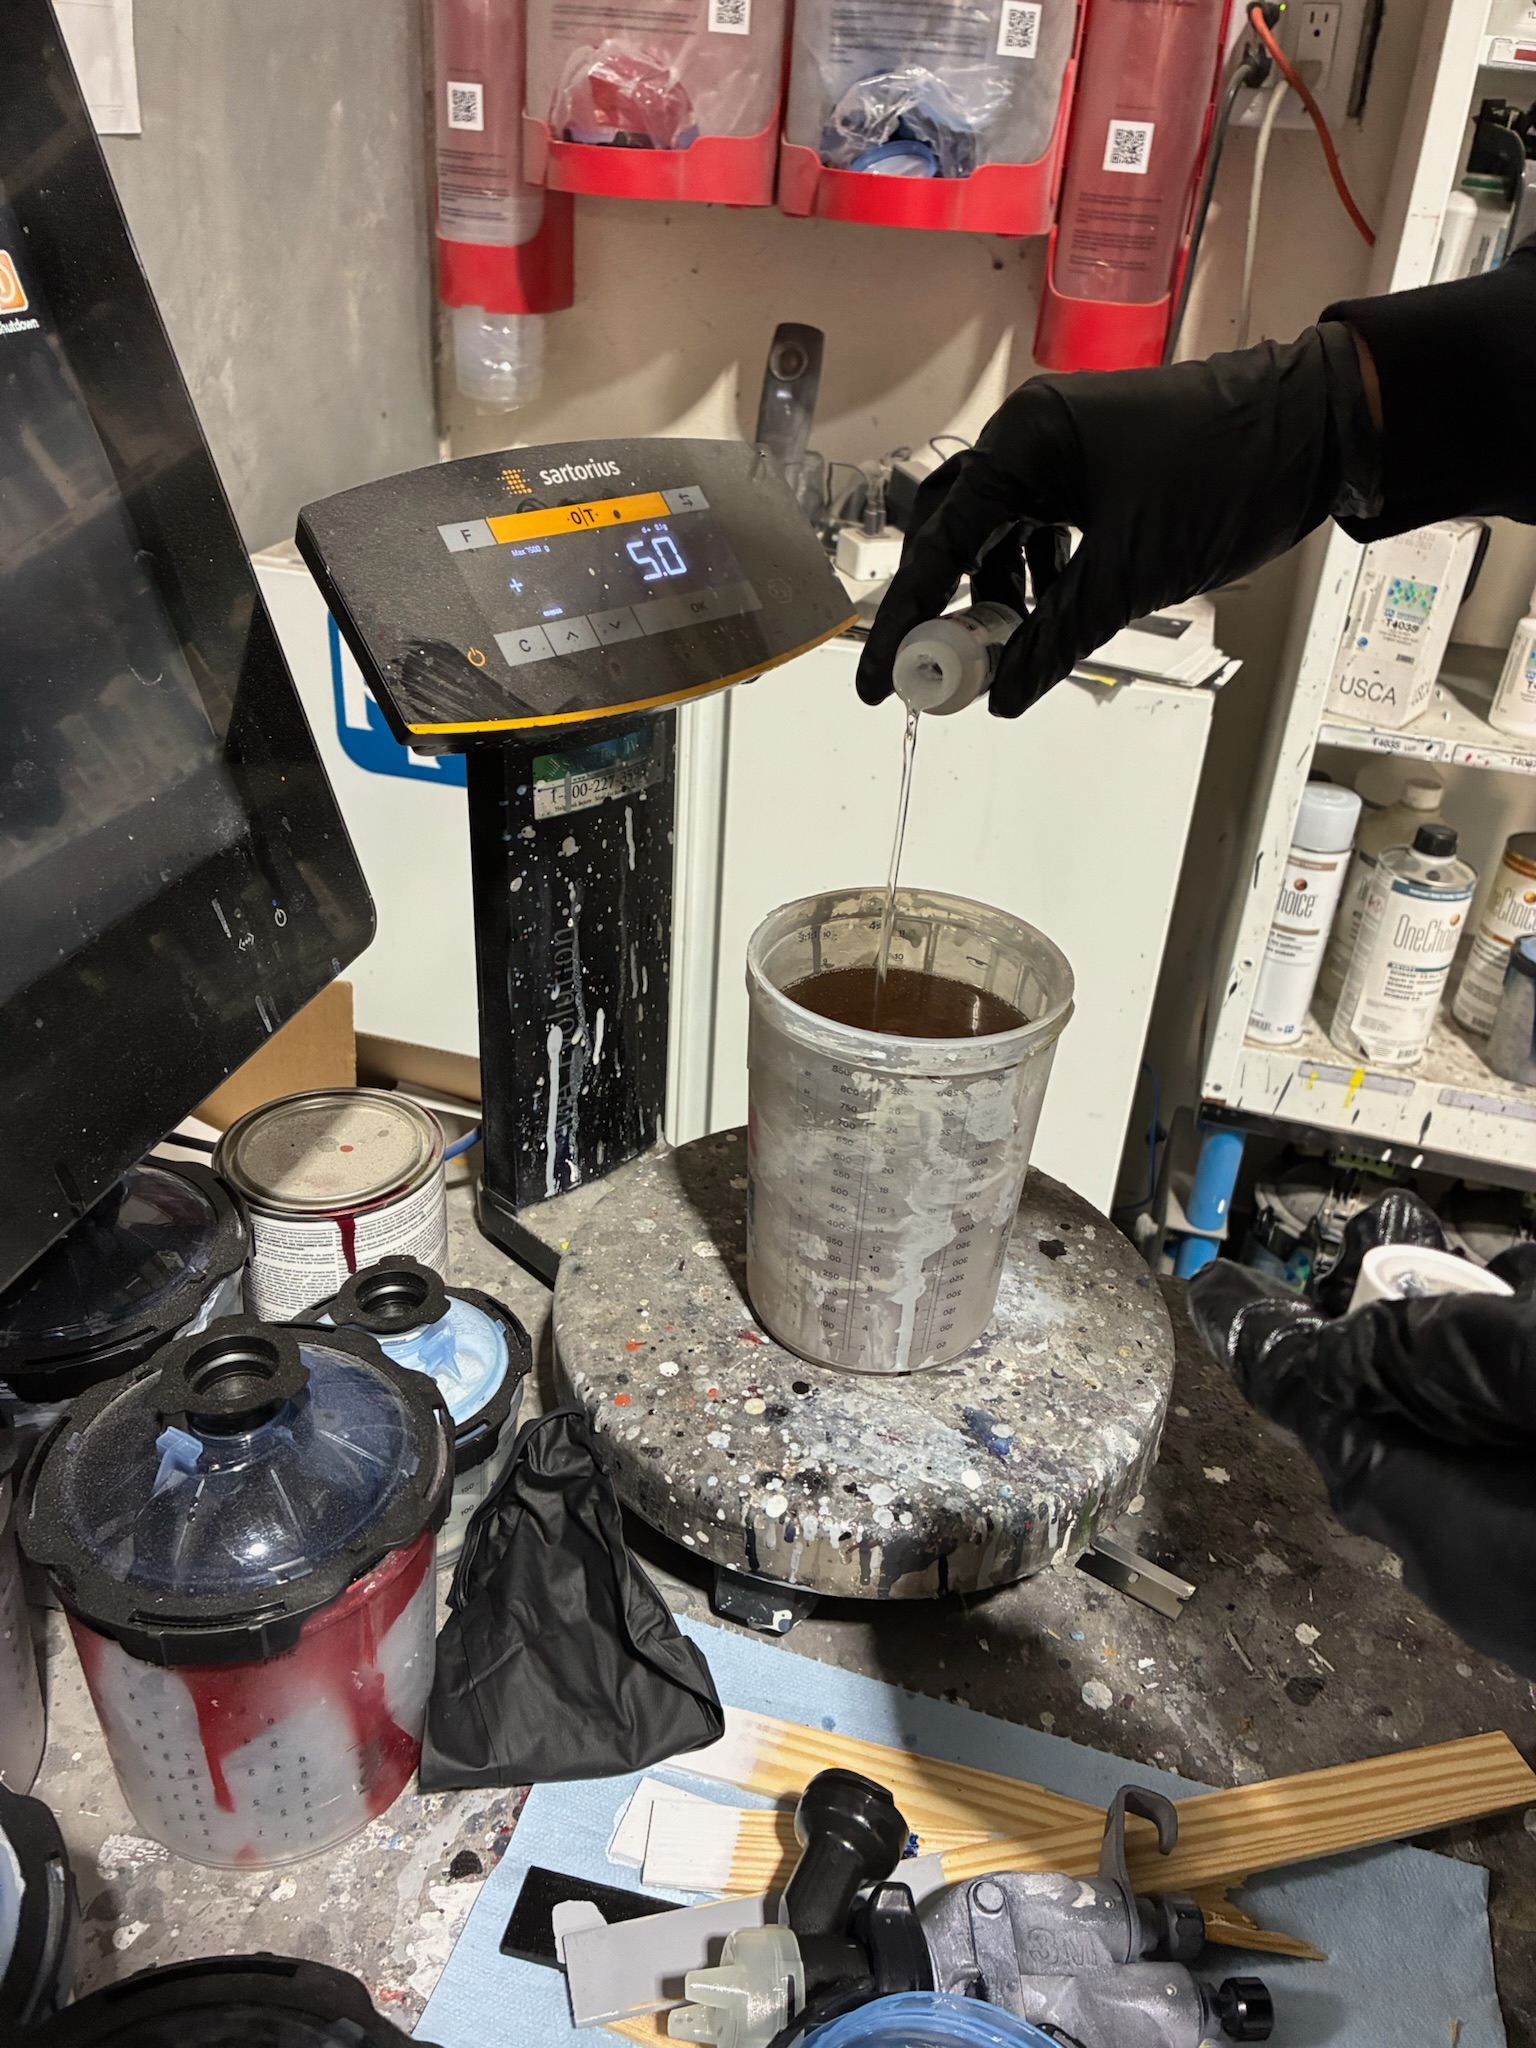
\includegraphics[
        width=2.35in,
        height=1.40in,
        keepaspectratio
    ]{spray_topcoat_prep}
};
\draw[RuleGray,line width=0.55pt,rounded corners=4pt]
    ($(current page.north west)+(0.43in,-1.91in)$)
    rectangle
    ($(current page.north west)+(2.98in,-3.40in)$);

% Image 2
\node[anchor=center,inner sep=0pt]
at ($(current page.north west)+(4.375in,-2.655in)$)
{
    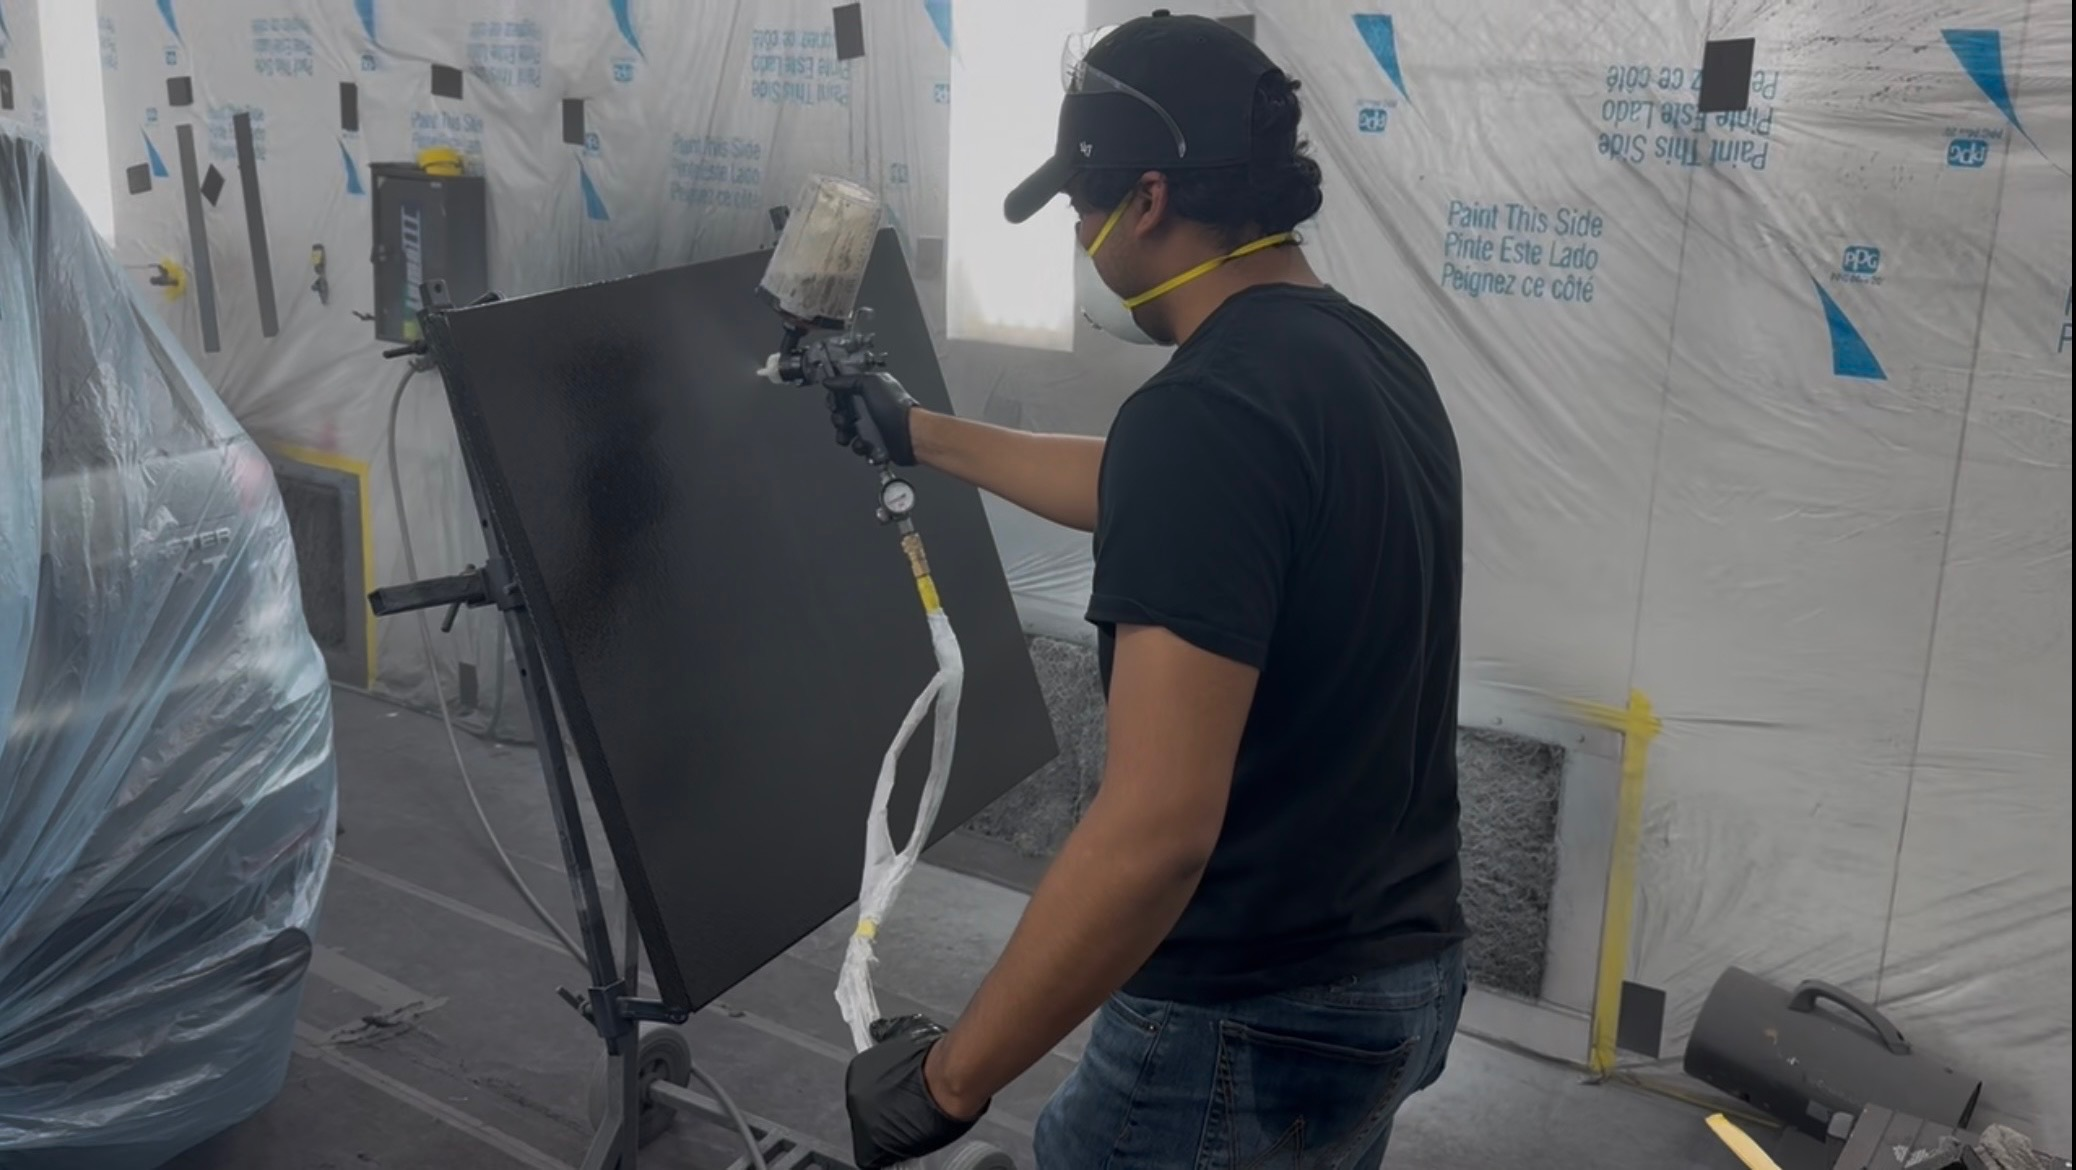
\includegraphics[
        width=2.35in,
        height=1.40in,
        keepaspectratio
    ]{spraying_topcoat}
};
\draw[RuleGray,line width=0.55pt,rounded corners=4pt]
    ($(current page.north west)+(3.10in,-1.91in)$)
    rectangle
    ($(current page.north west)+(5.65in,-3.40in)$);

% Image 3
\node[anchor=center,inner sep=0pt]
at ($(current page.north west)+(7.045in,-2.655in)$)
{
    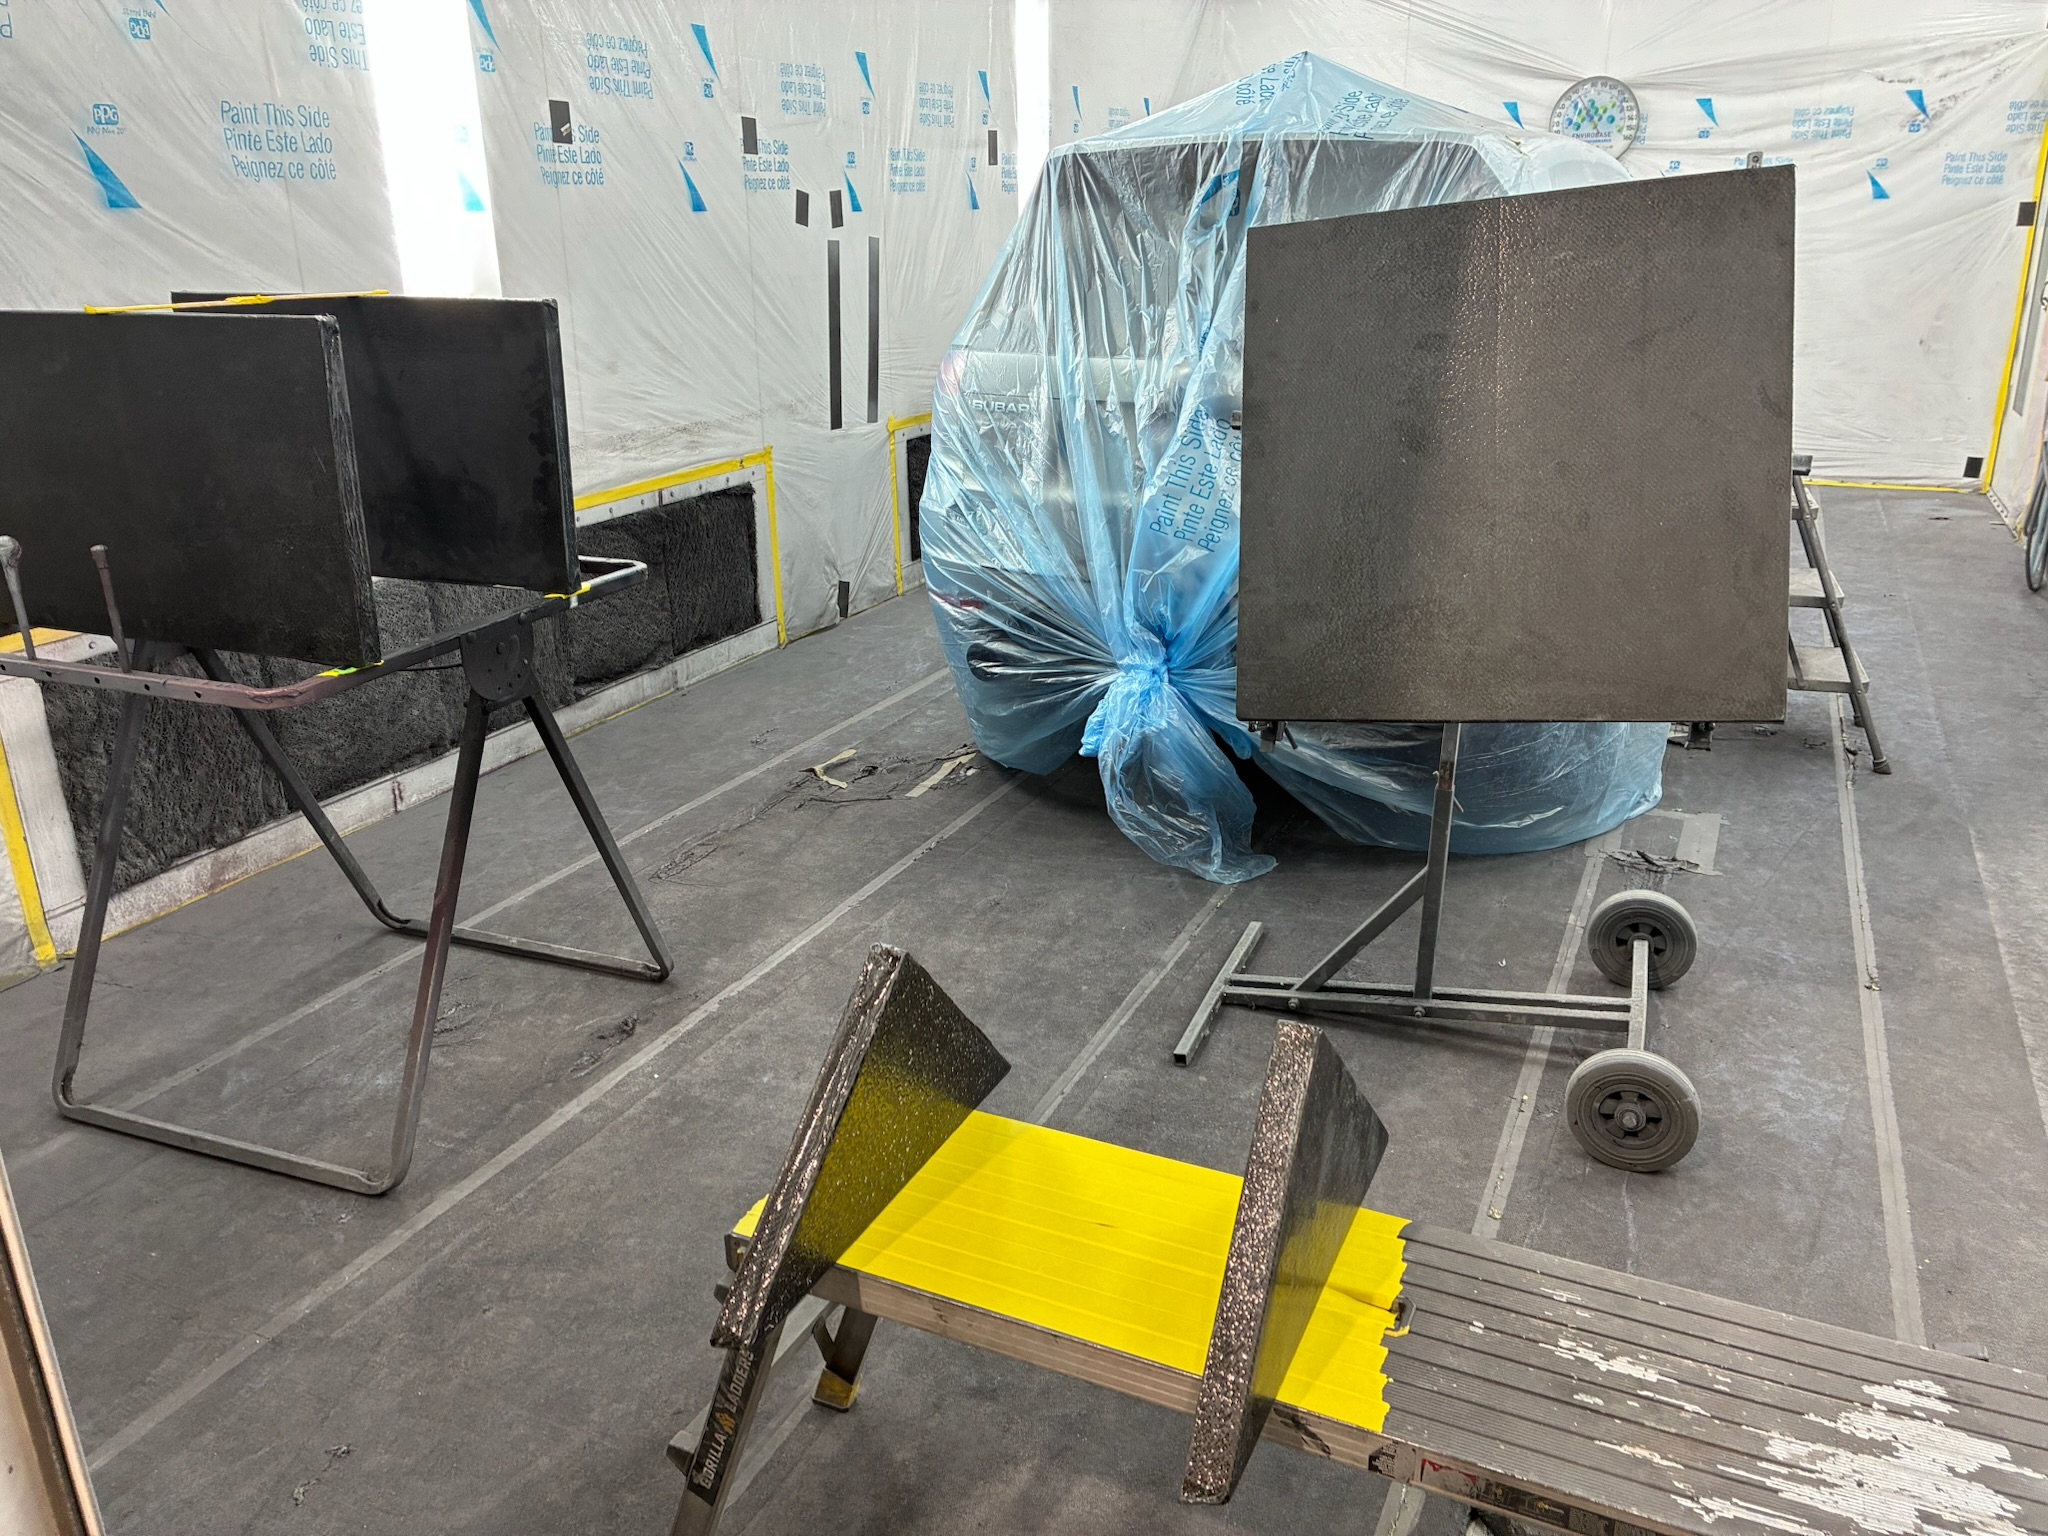
\includegraphics[
        width=2.35in,
        height=1.40in,
        keepaspectratio
    ]{topcoat_setup_apparatus}
};
\draw[RuleGray,line width=0.55pt,rounded corners=4pt]
    ($(current page.north west)+(5.77in,-1.91in)$)
    rectangle
    ($(current page.north west)+(8.32in,-3.40in)$);

% Image 4
\node[anchor=center,inner sep=0pt]
at ($(current page.north west)+(9.50in,-2.655in)$)
{
    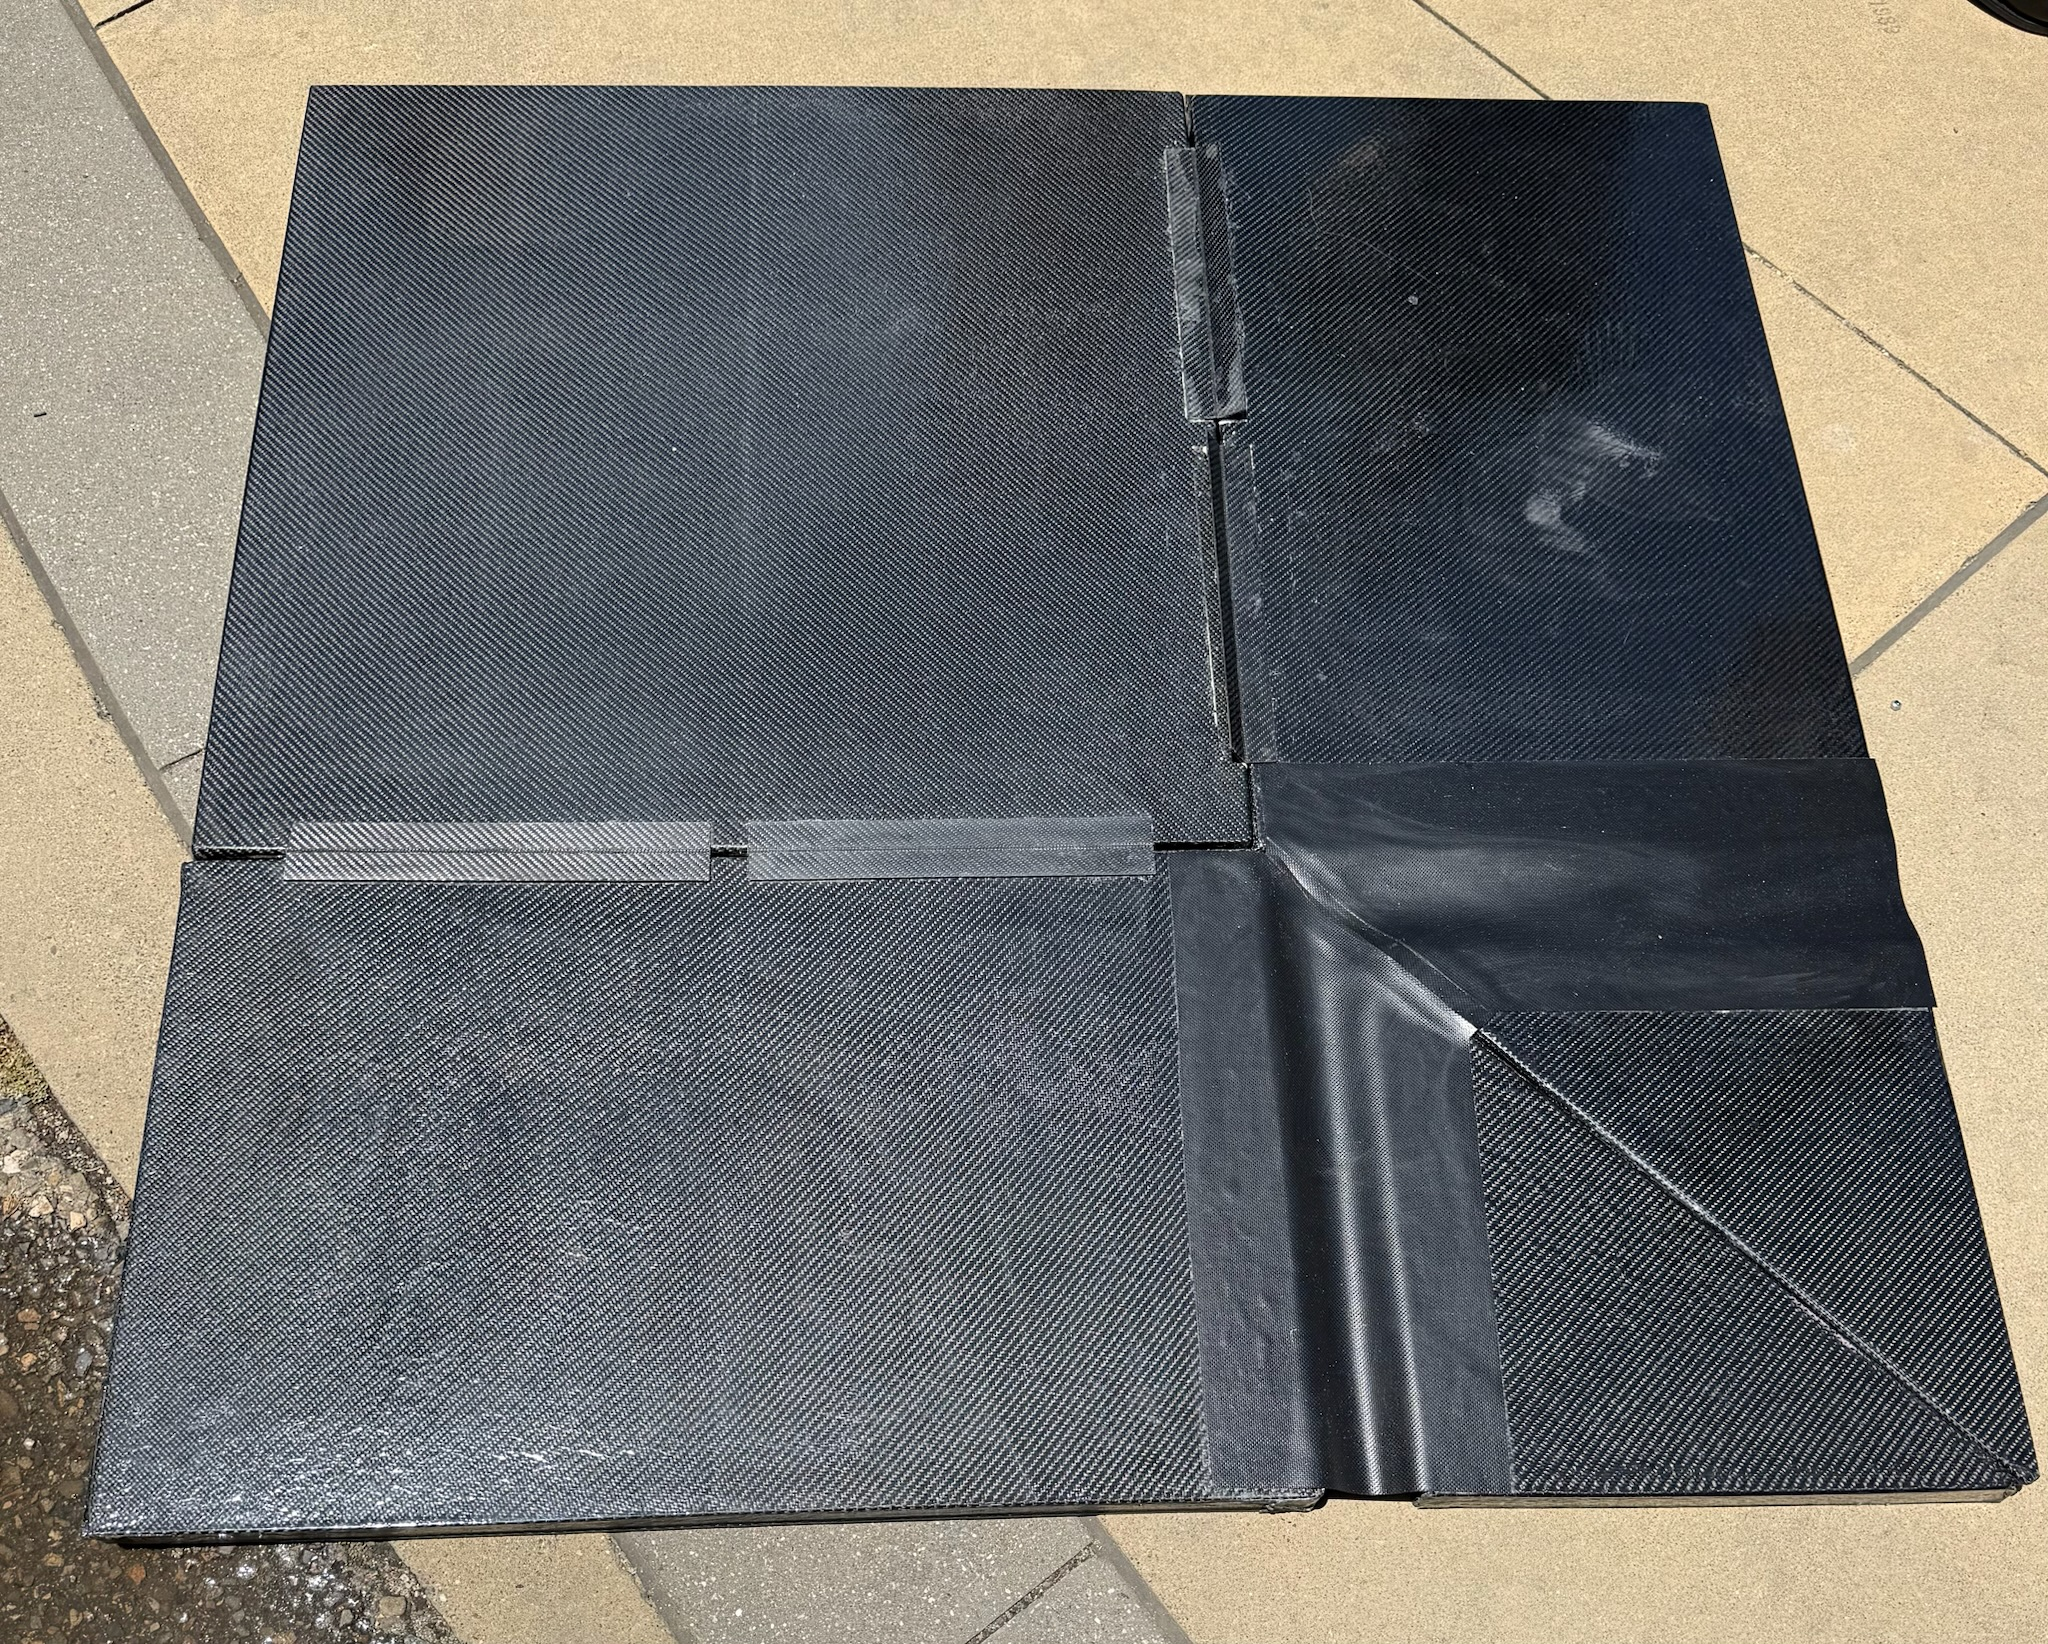
\includegraphics[
        width=2.35in,
        height=1.40in,
        keepaspectratio
    ]{refined_final_toro_cover_partial_carbon_model}
};
\draw[RuleGray,line width=0.55pt,rounded corners=4pt]
    ($(current page.north west)+(8.44in,-1.91in)$)
    rectangle
    ($(current page.north east)+(-0.42in,-3.40in)$);

% Captions
\node[anchor=north,text=Muted,font=\sffamily\fontsize{6.7}{7.3}\selectfont]
at ($(current page.north west)+(1.705in,-3.45in)$)
{Topcoat material preparation};

\node[anchor=north,text=Muted,font=\sffamily\fontsize{6.7}{7.3}\selectfont]
at ($(current page.north west)+(4.375in,-3.45in)$)
{Automotive-booth topcoat application};

\node[anchor=north,text=Muted,font=\sffamily\fontsize{6.7}{7.3}\selectfont]
at ($(current page.north west)+(7.045in,-3.45in)$)
{Coated panels drying after application};

\node[anchor=north,text=Muted,font=\sffamily\fontsize{6.7}{7.3}\selectfont]
at ($(current page.north west)+(9.50in,-3.45in)$)
{Partial carbon manufacturing model};

% Environmental rationale
\fill[SoftGold,rounded corners=4pt]
    ($(current page.north west)+(0.43in,-3.73in)$)
    rectangle
    ($(current page.north east)+(-0.42in,-4.76in)$);

\node[
    anchor=north west,
    align=left,
    text width=9.75in,
    text=Ink,
    font=\fontsize{7.05}{8.25}\selectfont
]
at ($(current page.north west)+(0.65in,-3.89in)$)
{
Because the sponsor required a carbon-fiber cover for outdoor use near chlorinated water,
environmental protection became a functional requirement rather than a cosmetic finish.
I selected and personally sprayed a UV-resistant Sunshield topcoat to seal minor laminate
porosity, reduce moisture ingress, preserve the carbon appearance, limit UV degradation of
the epoxy matrix, and isolate the composite surface from nearby metallic hardware.
};

% Results title
\node[
    anchor=north west,
    text=DeepGreen,
    font=\sffamily\bfseries\fontsize{8.0}{8.7}\selectfont
]
at ($(current page.north west)+(0.43in,-4.94in)$)
{FUNCTIONAL PROTOTYPE RESULTS};

% ------------------------------------------------------------
% Matched lower panels — larger type and improved allocation
% ------------------------------------------------------------

% Left results panel
\fill[SoftGreen,rounded corners=5pt]
    ($(current page.north west)+(0.43in,-5.22in)$)
    rectangle
    ($(current page.north west)+(5.98in,-7.39in)$);

\draw[RuleGray,line width=0.65pt,rounded corners=5pt]
    ($(current page.north west)+(0.43in,-5.22in)$)
    rectangle
    ($(current page.north west)+(5.98in,-7.39in)$);

\fill[DeepGreen,rounded corners=5pt]
    ($(current page.north west)+(0.43in,-5.22in)$)
    rectangle
    ($(current page.north west)+(5.98in,-5.58in)$);

\fill[DeepGreen]
    ($(current page.north west)+(0.43in,-5.40in)$)
    rectangle
    ($(current page.north west)+(5.98in,-5.58in)$);

\node[anchor=west,text=white,
      font=\sffamily\bfseries\fontsize{7.0}{7.6}\selectfont]
at ($(current page.north west)+(0.66in,-5.40in)$)
{SPECIFICATION};

\node[anchor=west,text=white,
      font=\sffamily\bfseries\fontsize{7.0}{7.6}\selectfont]
at ($(current page.north west)+(3.02in,-5.40in)$)
{RESULT};

\node[anchor=east,text=white,
      font=\sffamily\bfseries\fontsize{7.0}{7.6}\selectfont]
at ($(current page.north west)+(5.55in,-5.40in)$)
{STATUS};

\node[
    anchor=north west,
    align=left,
    text width=2.15in,
    text=Ink,
    font=\bfseries\fontsize{7.15}{8.55}\selectfont
]
at ($(current page.north west)+(0.66in,-5.72in)$)
{
Deployment time\\[3.4pt]
Removal time\\[3.4pt]
Single-user operation\\[3.4pt]
Single-side operation\\[3.4pt]
Deployment steps\\[3.4pt]
Removal steps\\[3.4pt]
Weight\\[3.4pt]
Folded storage
};

\node[
    anchor=north west,
    align=left,
    text width=1.45in,
    text=Ink,
    font=\fontsize{7.15}{8.55}\selectfont
]
at ($(current page.north west)+(3.02in,-5.72in)$)
{
25.51 seconds\\[3.4pt]
37.22 seconds\\[3.4pt]
100\% successful\\[3.4pt]
75\% successful\\[3.4pt]
6.4 average\\[3.4pt]
9 average\\[3.4pt]
17 lb\\[3.4pt]
2.9' x 2.9' x 1.7'
};

\node[
    anchor=north east,
    align=right,
    text width=1.05in,
    text=DeepGreen,
    font=\sffamily\bfseries\fontsize{7.05}{8.55}\selectfont
]
at ($(current page.north west)+(5.55in,-5.72in)$)
{
PASS\\[3.4pt]
PASS\\[3.4pt]
PASS\\[3.4pt]
NEAR TARGET\\[3.4pt]
PASS\\[3.4pt]
PASS\\[3.4pt]
NEAR TARGET\\[3.4pt]
PASS
};

% Right takeaways panel — widened for easier reading
\fill[SoftGreen,rounded corners=5pt]
    ($(current page.north west)+(6.14in,-5.22in)$)
    rectangle
    ($(current page.north east)+(-0.42in,-7.39in)$);

\draw[RuleGray,line width=0.65pt,rounded corners=5pt]
    ($(current page.north west)+(6.14in,-5.22in)$)
    rectangle
    ($(current page.north east)+(-0.42in,-7.39in)$);

\fill[DeepGreen,rounded corners=5pt]
    ($(current page.north west)+(6.14in,-5.22in)$)
    rectangle
    ($(current page.north east)+(-0.42in,-5.58in)$);

\fill[DeepGreen]
    ($(current page.north west)+(6.14in,-5.40in)$)
    rectangle
    ($(current page.north east)+(-0.42in,-5.58in)$);

\node[anchor=west,text=white,
      font=\sffamily\bfseries\fontsize{7.1}{7.7}\selectfont]
at ($(current page.north west)+(6.38in,-5.40in)$)
{ENGINEERING TAKEAWAYS};

\node[
    anchor=north west,
    align=left,
    text width=4.02in,
    text=Ink,
    font=\fontsize{6.75}{7.85}\selectfont
]
at ($(current page.north west)+(6.38in,-5.72in)$)
{
\textbf{Manufacturing first.}
Composite manufacturing constraints should guide the product architecture from the beginning.\\[4.5pt]
\textbf{Prioritize deliberately.}
Competing requirements must be balanced intentionally instead of maximizing every objective.\\[4.5pt]
\textbf{Lead through the process.}
Clear procedures, calm communication, and respect for teammates' strengths were essential during fabrication.\\[4.5pt]
\textbf{Next iteration.}
Reduce weight, refine the fabric-hinge fold lines, and improve panel-edge clearance.
};

% Compact concluding pathway
\node[
    anchor=center,
    align=center,
    text=PolyGold,
    font=\sffamily\bfseries\fontsize{6.3}{6.9}\selectfont
]
at ($(current page.north)+(3.06in,-7.18in)$)
{PROTOTYPE \faArrowRight\ DESIGN REFINEMENT
\faArrowRight\ REPEATABLE MANUFACTURING
\faArrowRight\ PRODUCT};

% Validation resources
\node[
    anchor=north,
    align=center,
    text=DeepGreen,
    font=\sffamily\bfseries\fontsize{6.6}{7.2}\selectfont
]
at ($(current page.north)+(0,-7.58in)$)
{\href{\ToroDeploymentLink}{\faPlayCircle\ DEPLOYMENT}
\hspace{18pt}
\href{\ToroRemovalLink}{\faPlayCircle\ REMOVAL / FOLDING}
\hspace{18pt}
\href{\ToroPosterLink}{\faFilePdf\ EXPO POSTER}
\hspace{18pt}
\href{\ToroReportLink}{\faFilePdf\ FINAL REPORT}};

% Footer
\node[
    anchor=south west,
    text=white,
    font=\sffamily\bfseries\fontsize{7.1}{7.7}\selectfont
]
at ($(current page.south west)+(0.42in,0.17in)$)
{\faArrowLeft\ MANUFACTURING-DRIVEN DESIGN};

\node[
    anchor=south,
    text=white,
    font=\sffamily\fontsize{7.0}{7.6}\selectfont
]
at ($(current page.south)+(0,0.17in)$)
{TORO COVER \hspace{6pt} 3 / 3};

\node[
    anchor=south east,
    text=white,
    font=\sffamily\bfseries\fontsize{7.1}{7.7}\selectfont
]
at ($(current page.south east)+(-0.42in,0.17in)$)
{NEXT PROJECT \faArrowRight};

\end{tikzpicture}
\input{paddle}
\clearpage
.
% 2. In main.tex, place 
% ============================================================
% TORO COVER — THREE-PAGE PORTFOLIO CASE STUDY
% Pages 3–5 of the complete portfolio
%
% IMPORTANT:
% 1. This file must NOT contain \documentclass, \begin{document},
%    \end{document}, or \input{toro}.
% 2. In main.tex, place \input{toro} before \end{document}.
% 3. Image references use the original Overleaf base filenames
%    without extensions.
% ============================================================



% ============================================================
% CLICKABLE PROJECT RESOURCES
% All links use the exact Google Drive resources supplied.
% ============================================================
\providecommand{\ToroDrawingLink}{https://drive.google.com/file/d/1A7-7wMnRNLuQDaTgxeuUCBsGNqyXzOGV/view?usp=sharing}
\providecommand{\ToroDimensionsLink}{https://drive.google.com/file/d/13sw3BNJvE8GdzlRffxoF2n5r9Gzxide7/view?usp=sharing}
\providecommand{\ToroProblemLink}{https://drive.google.com/file/d/1zHtl8zrb13F1yeN74ptawpfS5UM_xsuw/view?usp=drive_link}
\providecommand{\ToroReportLink}{https://drive.google.com/file/d/1ULZ-P46lFsC2x29ZfmRVIKgYnr9o8hMt/view?usp=drive_link}
\providecommand{\ToroPosterLink}{https://drive.google.com/file/d/1vKiKaJUcHQb_db-FkZnRF6EvtuM4hKyS/view?usp=drive_link}
\providecommand{\ToroDeploymentLink}{https://drive.google.com/file/d/1XJx34o80_mZPTl7xy93HtWAgtS3ThhvY/view?usp=drive_link}
\providecommand{\ToroRemovalLink}{https://drive.google.com/file/d/1O7xYeyB67NUwT-j1B1HeiCcHnZDYjk6_/view?usp=drive_link}

% ============================================================
% PAGE 1 — PROJECT OVERVIEW, OWNERSHIP, AND ARCHITECTURE
% ============================================================

\clearpage
\thispagestyle{empty}
\hypertarget{toro}{}
\null

\begin{tikzpicture}[remember picture,overlay]

% Background
\fill[white]
    (current page.south west)
    rectangle
    (current page.north east);

% Page bars
\fill[DeepGreen]
    (current page.north west)
    rectangle
    ($(current page.north east)+(0,-0.095in)$);

\fill[PolyGold]
    ($(current page.north west)+(0,-0.095in)$)
    rectangle
    ($(current page.north east)+(0,-0.14in)$);

\fill[DeepGreen]
    (current page.south west)
    rectangle
    ($(current page.south east)+(0,0.36in)$);

\fill[PolyGold]
    ($(current page.south west)+(0,0.36in)$)
    rectangle
    ($(current page.south east)+(0,0.405in)$);

% Header
\node[
    anchor=north west,
    text=PolyGold,
    font=\sffamily\bfseries\fontsize{8.1}{8.7}\selectfont
]
at ($(current page.north west)+(0.42in,-0.39in)$)
{01 COMPOSITES \hspace{5pt}/\hspace{5pt} PROJECT 01};

\node[
    anchor=north west,
    text=DeepGreen,
    font=\bfseries\fontsize{23.5}{24.5}\selectfont
]
at ($(current page.north west)+(0.40in,-0.67in)$)
{TORO CARBON FIBER SAFETY COVER};

\node[
    anchor=north west,
    text=Muted,
    font=\sffamily\fontsize{8.4}{9.2}\selectfont
]
at ($(current page.north west)+(0.42in,-1.12in)$)
{Cal Poly Composites Laboratory \hspace{7pt}\textbullet\hspace{7pt}
Team Project \hspace{7pt}\textbullet\hspace{7pt}
Fall--Spring 2026 \hspace{7pt}\textbullet\hspace{7pt}
San Luis Obispo, California};

\fill[PolyGold]
    ($(current page.north west)+(0.42in,-1.37in)$)
    rectangle
    ($(current page.north west)+(6.1in,-1.325in)$);

% Challenge text
\node[
    anchor=north west,
    text=DeepGreen,
    font=\sffamily\bfseries\fontsize{8.1}{8.8}\selectfont
]
at ($(current page.north west)+(0.43in,-1.61in)$)
{THE CHALLENGE};

\node[
    anchor=north west,
    align=left,
    text width=4.47in,
    text=Ink,
    font=\fontsize{8.05}{9.65}\selectfont
]
at ($(current page.north west)+(0.43in,-1.84in)$)
{
Develop a lightweight cover for a 6 ft by 6 ft in-ground spa
that could be deployed by one person, stored compactly,
provide insulation, resist a poolside environment, and maintain
a refined appearance. The sponsor supplied an ambitious but
intentionally broad project statement, requiring the team to
define the product architecture, priorities, manufacturing
strategy, and realistic path toward future commercialization.
};

% Role box
\fill[SoftGold,rounded corners=5pt]
    ($(current page.north west)+(0.42in,-2.88in)$)
    rectangle
    ($(current page.north west)+(4.98in,-4.58in)$);

\fill[PolyGold]
    ($(current page.north west)+(0.42in,-2.88in)$)
    rectangle
    ($(current page.north west)+(0.52in,-4.58in)$);

\node[
    anchor=north west,
    text=DeepGreen,
    font=\sffamily\bfseries\fontsize{8.1}{8.8}\selectfont
]
at ($(current page.north west)+(0.66in,-3.02in)$)
{MY ROLE — DESIGN \& MANUFACTURING LEAD};

\node[
    anchor=north west,
    align=left,
    text width=4.02in,
    text=Ink,
    font=\fontsize{7.05}{8.15}\selectfont
]
at ($(current page.north west)+(0.66in,-3.27in)$)
{
\textbullet\ Modeled every custom part and the complete assembly\\[1.5pt]
\textbullet\ Produced the engineering drawing package independently\\[1.5pt]
\textbullet\ Developed the composite-panel manufacturing process\\[1.5pt]
\textbullet\ Created all waterjet DXFs and manufacturing geometry\\[1.5pt]
\textbullet\ Trained teammates in wet layup and vacuum bagging\\[1.5pt]
\textbullet\ Presented feasibility, scope, and tradeoffs to the sponsor
};

% Large deployed foam-model image
\node[anchor=center,inner sep=0pt]
at ($(current page.north west)+(8.00in,-3.04in)$)
{
    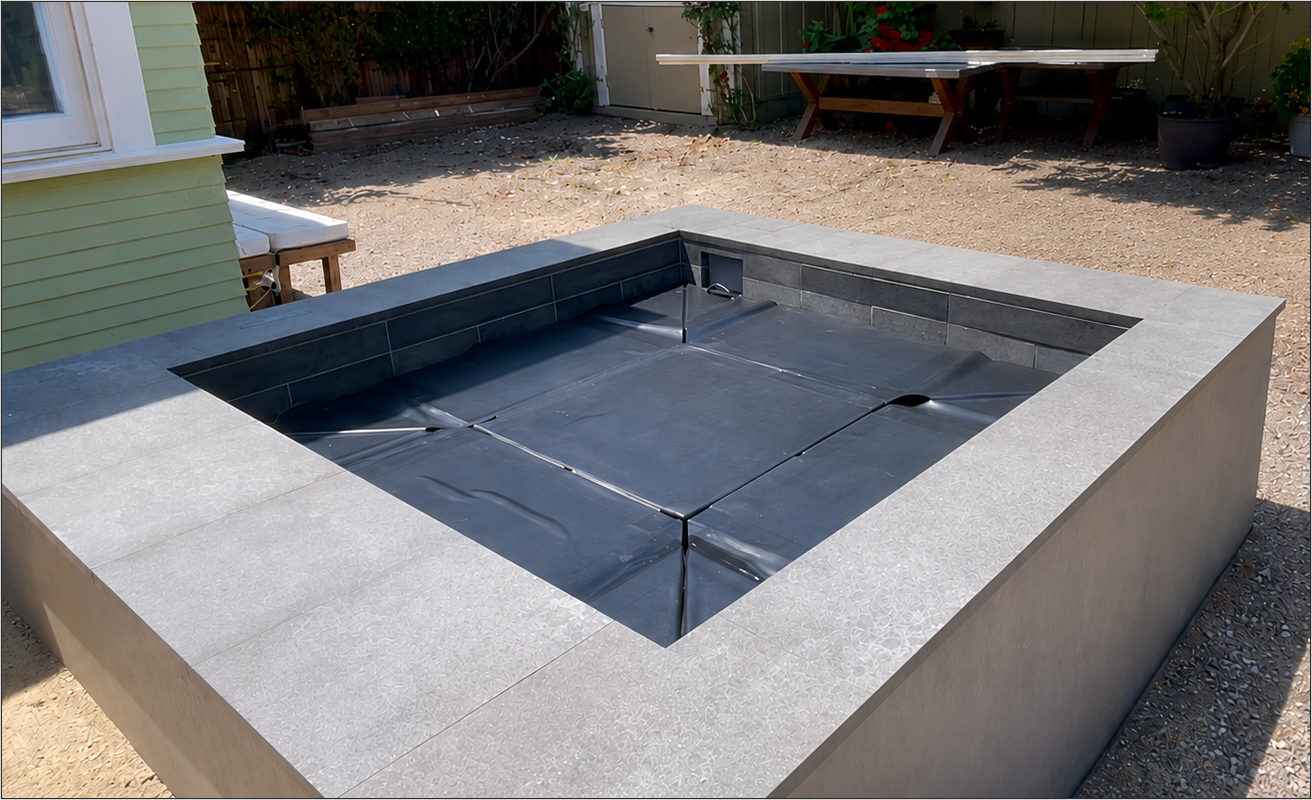
\includegraphics[
        width=5.55in,
        height=2.78in,
        keepaspectratio
    ]{deployed_functional_prototype}
};

\draw[DeepGreen,line width=0.8pt,rounded corners=7pt]
    ($(current page.north west)+(5.16in,-1.61in)$)
    rectangle
    ($(current page.north east)+(-0.42in,-4.47in)$);

\node[
    anchor=north west,
    text=Muted,
    font=\sffamily\fontsize{6.2}{6.9}\selectfont
]
at ($(current page.north west)+(5.18in,-4.54in)$)
{Functional foam model deployed over the sponsor's in-ground spa.};

% Image-strip title
\node[
    anchor=north west,
    text=DeepGreen,
    font=\sffamily\bfseries\fontsize{8.1}{8.8}\selectfont
]
at ($(current page.north west)+(0.43in,-4.78in)$)
{PRODUCT DEVELOPMENT AND FINAL ARCHITECTURE};

% Five-image development strip — CAD-first sequence
% Image 1: topside CAD
\node[anchor=center,inner sep=0pt]
at ($(current page.north west)+(1.47in,-5.73in)$)
{
    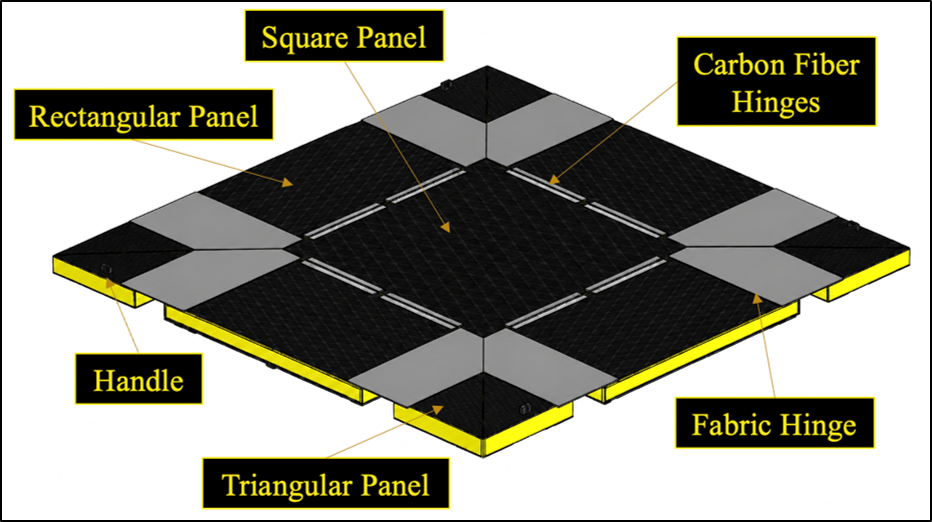
\includegraphics[
        width=1.92in,
        height=1.30in,
        keepaspectratio
    ]{Toro_Cover_topside_Cad}
};
\draw[RuleGray,line width=0.55pt,rounded corners=4pt]
    ($(current page.north west)+(0.43in,-5.04in)$)
    rectangle
    ($(current page.north west)+(2.51in,-6.43in)$);

% Image 2: underside CAD
\node[anchor=center,inner sep=0pt]
at ($(current page.north west)+(3.66in,-5.73in)$)
{
    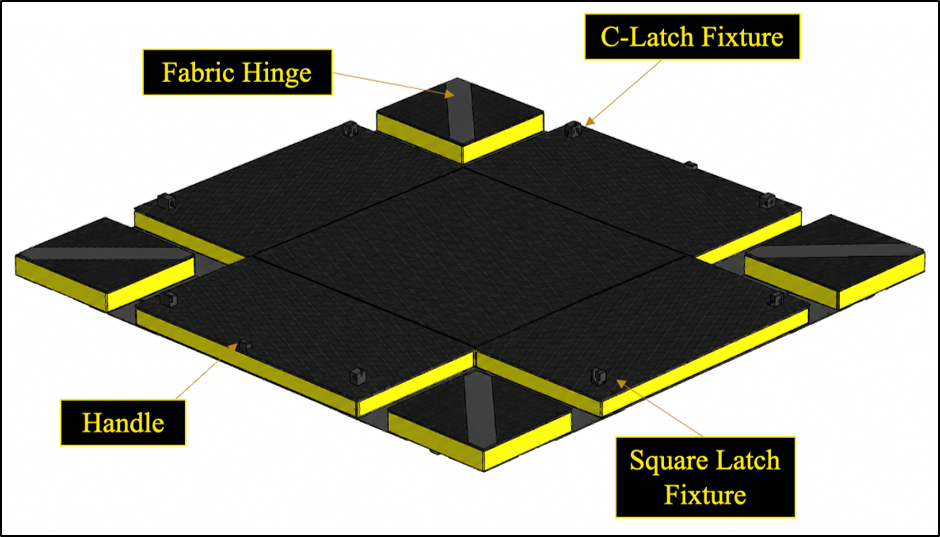
\includegraphics[
        width=1.92in,
        height=1.30in,
        keepaspectratio
    ]{toro_cover_underside_cad}
};
\draw[RuleGray,line width=0.55pt,rounded corners=4pt]
    ($(current page.north west)+(2.62in,-5.04in)$)
    rectangle
    ($(current page.north west)+(4.70in,-6.43in)$);

% Image 3: folded CAD
\node[anchor=center,inner sep=0pt]
at ($(current page.north west)+(5.85in,-5.73in)$)
{
    \includegraphics[
        width=1.92in,
        height=1.30in,
        keepaspectratio
    ]{\detokenize{Toro_Cover_folded Configuration}}
};
\draw[RuleGray,line width=0.55pt,rounded corners=4pt]
    ($(current page.north west)+(4.81in,-5.04in)$)
    rectangle
    ($(current page.north west)+(6.89in,-6.43in)$);

% Image 4: dual-use product concept
\node[anchor=center,inner sep=0pt]
at ($(current page.north west)+(8.04in,-5.73in)$)
{
    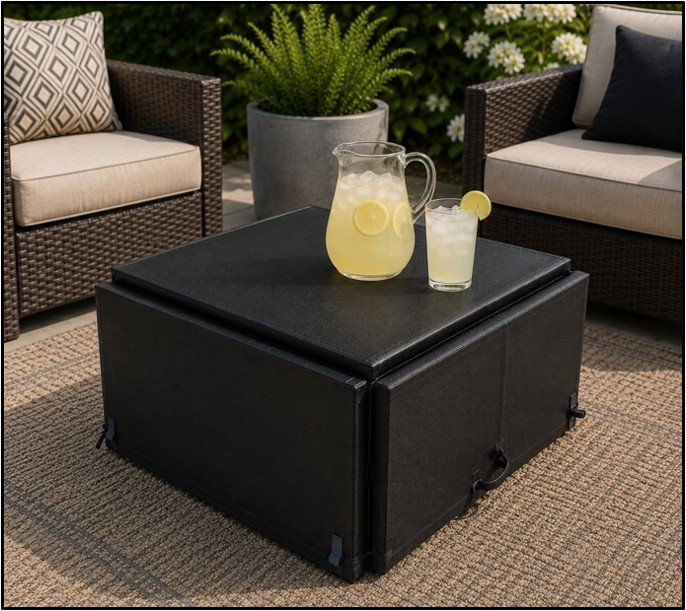
\includegraphics[
        width=1.92in,
        height=1.30in,
        keepaspectratio
    ]{generative_AI_concept_toro_cover_art}
};
\draw[RuleGray,line width=0.55pt,rounded corners=4pt]
    ($(current page.north west)+(7.00in,-5.04in)$)
    rectangle
    ($(current page.north west)+(9.08in,-6.43in)$);

% Image 5: folded foam functional prototype
% The portrait photograph is deliberately clipped to the landscape frame
% so the ottoman fills the card without extending beyond its border.
\begin{scope}
\clip[rounded corners=4pt]
    ($(current page.north west)+(9.19in,-5.04in)$)
    rectangle
    ($(current page.north east)+(-0.43in,-6.43in)$);

% Keep the original image proportions and center it within the existing card.
\node[anchor=center,inner sep=0pt]
at ($(current page.north west)+(9.88in,-5.735in)$)
{
    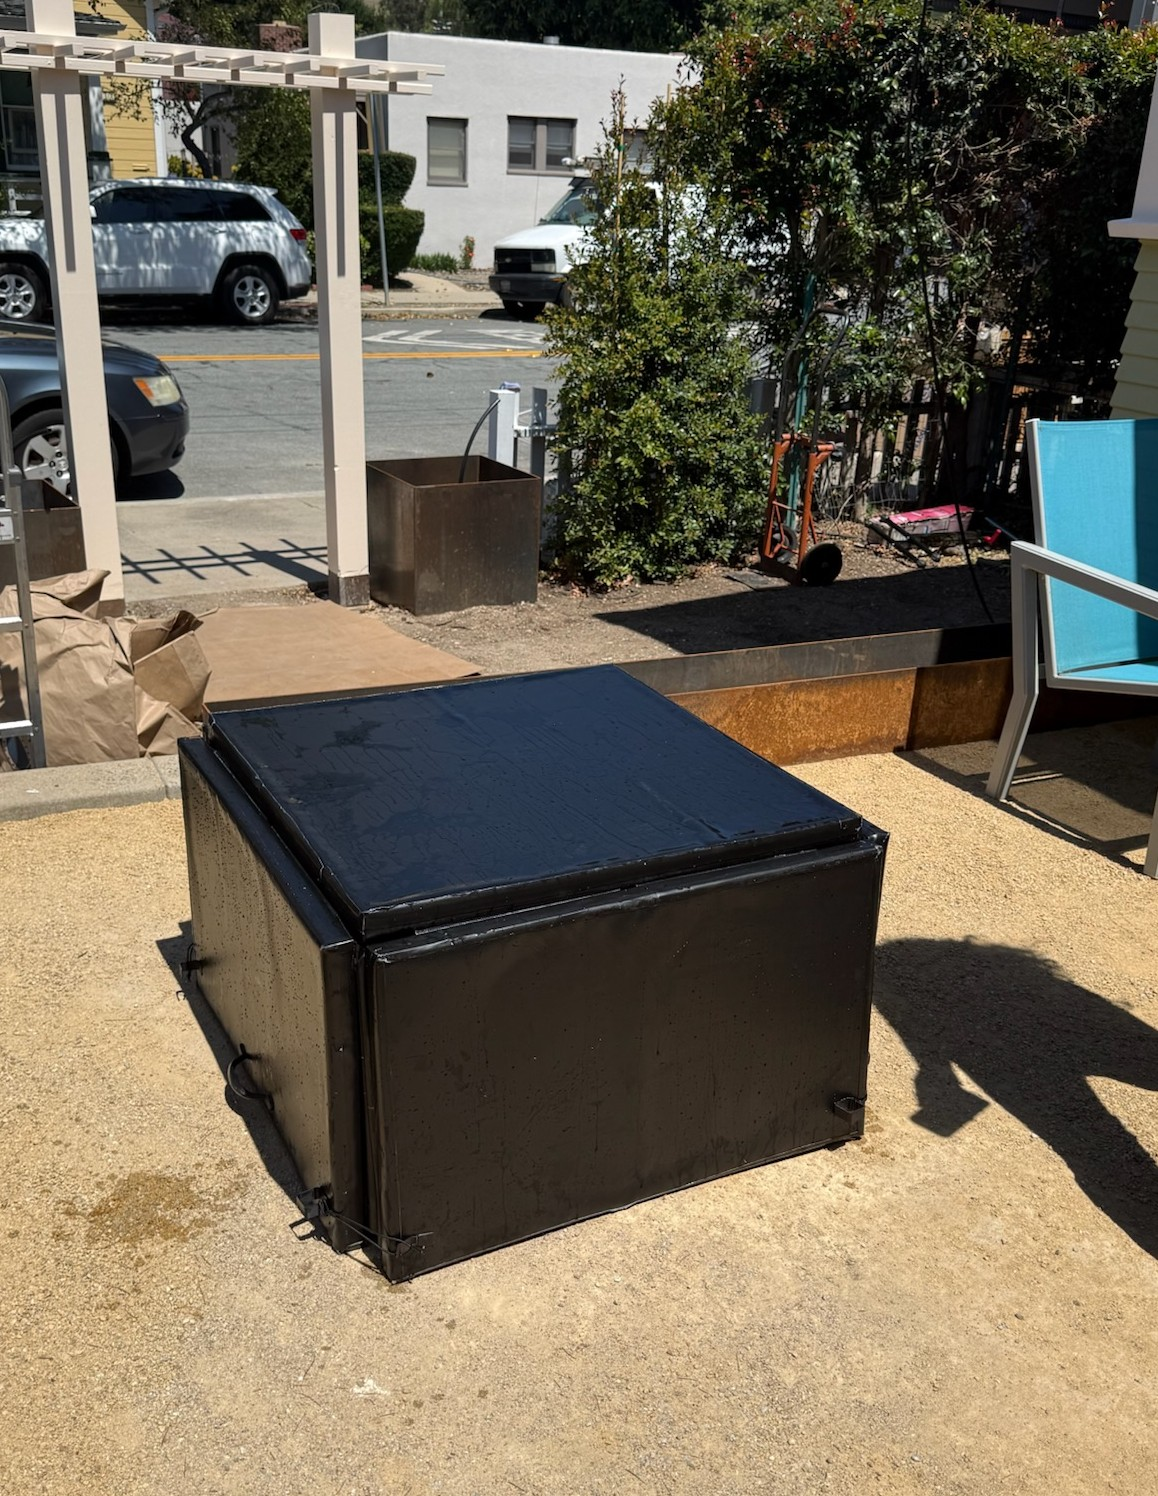
\includegraphics[
        width=1.58in,
        height=1.28in,
        keepaspectratio
    ]{foam_model_folded_backyard_image}
};
\end{scope}

\draw[RuleGray,line width=0.55pt,rounded corners=4pt]
    ($(current page.north west)+(9.19in,-5.04in)$)
    rectangle
    ($(current page.north east)+(-0.43in,-6.43in)$);

% Larger captions
\node[anchor=north,align=center,text width=1.95in,text=Muted,
      font=\sffamily\fontsize{6.8}{7.4}\selectfont]
at ($(current page.north west)+(1.47in,-6.49in)$)
{Topside panel architecture};

\node[anchor=north,align=center,text width=1.95in,text=Muted,
      font=\sffamily\fontsize{6.8}{7.4}\selectfont]
at ($(current page.north west)+(3.66in,-6.49in)$)
{Underside hinge architecture};

\node[anchor=north,align=center,text width=1.95in,text=Muted,
      font=\sffamily\fontsize{6.8}{7.4}\selectfont]
at ($(current page.north west)+(5.85in,-6.49in)$)
{Folded CAD configuration};

\node[anchor=north,align=center,text width=1.95in,text=Muted,
      font=\sffamily\fontsize{6.8}{7.4}\selectfont]
at ($(current page.north west)+(8.04in,-6.49in)$)
{Dual-use product vision};

\node[anchor=north,align=center,text width=1.95in,text=Muted,
      font=\sffamily\fontsize{6.8}{7.4}\selectfont]
at ($(current page.north west)+(9.88in,-6.49in)$)
{Folded foam prototype};

% Page 1 resource bar — centered and non-repeated resources
\fill[Panel,rounded corners=4pt]
    ($(current page.north west)+(0.43in,-7.05in)$)
    rectangle
    ($(current page.north east)+(-0.43in,-7.64in)$);
\draw[RuleGray,line width=0.5pt,rounded corners=4pt]
    ($(current page.north west)+(0.43in,-7.05in)$)
    rectangle
    ($(current page.north east)+(-0.43in,-7.64in)$);

\node[
    anchor=center,
    align=center,
    text=DeepGreen,
    font=\sffamily\bfseries\fontsize{6.9}{7.5}\selectfont
]
at ($(current page.north)+(0,-7.345in)$)
{\href{\ToroDrawingLink}{\faDraftingCompass\ DRAWING PACKAGE}
\hspace{24pt}
\href{\ToroDimensionsLink}{\faImage\ DIMENSION STUDY}
\hspace{24pt}
\href{\ToroProblemLink}{\faFileImage\ PROBLEM STATEMENT}};

% Footer
\node[
    anchor=south west,
    text=white,
    font=\sffamily\bfseries\fontsize{7.1}{7.7}\selectfont
]
at ($(current page.south west)+(0.42in,0.17in)$)
{\hyperlink{composites}{\faArrowLeft\ COMPOSITES}};

\node[
    anchor=south,
    text=white,
    font=\sffamily\fontsize{7.0}{7.6}\selectfont
]
at ($(current page.south)+(0,0.17in)$)
{TORO COVER \hspace{6pt} 1 / 3};

\node[
    anchor=south east,
    text=white,
    font=\sffamily\bfseries\fontsize{7.1}{7.7}\selectfont
]
at ($(current page.south east)+(-0.42in,0.17in)$)
{MANUFACTURING-DRIVEN DESIGN \faArrowRight};

\end{tikzpicture}


% ============================================================
% PAGE 2 — MANUFACTURING-DRIVEN DESIGN
% ============================================================

\clearpage
\thispagestyle{empty}
\hypertarget{toro-manufacturing}{}
\null

\begin{tikzpicture}[remember picture,overlay]

% Background and bars
\fill[white]
    (current page.south west)
    rectangle
    (current page.north east);

\fill[DeepGreen]
    (current page.north west)
    rectangle
    ($(current page.north east)+(0,-0.095in)$);

\fill[PolyGold]
    ($(current page.north west)+(0,-0.095in)$)
    rectangle
    ($(current page.north east)+(0,-0.14in)$);

\fill[DeepGreen]
    (current page.south west)
    rectangle
    ($(current page.south east)+(0,0.36in)$);

\fill[PolyGold]
    ($(current page.south west)+(0,0.36in)$)
    rectangle
    ($(current page.south east)+(0,0.405in)$);

% Header
\node[
    anchor=north west,
    text=PolyGold,
    font=\sffamily\bfseries\fontsize{8.1}{8.7}\selectfont
]
at ($(current page.north west)+(0.42in,-0.39in)$)
{TORO COVER \hspace{5pt}/\hspace{5pt} DESIGN FOR MANUFACTURABILITY};

\node[
    anchor=north west,
    text=DeepGreen,
    font=\bfseries\fontsize{23}{24}\selectfont
]
at ($(current page.north west)+(0.40in,-0.67in)$)
{THE ENVELOPE METHOD};

\node[
    anchor=north west,
    text=Muted,
    font=\sffamily\fontsize{8.7}{9.6}\selectfont
]
at ($(current page.north west)+(0.42in,-1.12in)$)
{A one-layup process developed for unusually thick insulated composite sandwich panels};

\fill[PolyGold]
    ($(current page.north west)+(0.42in,-1.36in)$)
    rectangle
    ($(current page.north west)+(5.30in,-1.315in)$);

% Process explanation
\fill[SoftGold,rounded corners=5pt]
    ($(current page.north west)+(0.42in,-1.61in)$)
    rectangle
    ($(current page.north east)+(-0.42in,-2.90in)$);

\fill[PolyGold]
    ($(current page.north west)+(0.42in,-1.61in)$)
    rectangle
    ($(current page.north west)+(0.52in,-2.90in)$);

\node[
    anchor=north west,
    text=DeepGreen,
    font=\sffamily\bfseries\fontsize{7.9}{8.6}\selectfont
]
at ($(current page.north west)+(0.67in,-1.76in)$)
{PROCESS INNOVATION};

\node[
    anchor=north west,
    align=left,
    text width=9.55in,
    text=Ink,
    font=\fontsize{7.35}{8.75}\selectfont
]
at ($(current page.north west)+(0.67in,-2.02in)$)
{
Weight reduction and insulation were both essential, leading to the selection of an
XPS foam core. Because XPS could not tolerate composite heat-cure temperatures, prepreg
processing was not practical and the panels had to be manufactured by wet layup with a
room-temperature cure. To simplify this process, I waterjet-cut XPS perimeter strips from
excess foam and placed them around each core inside the vacuum enclosure. Under vacuum,
the top and bottom carbon skins met along the panel sides and compressed against this
border, eliminating a separate edge-banding layup and reducing corner pleating.
};

% Workflow title
\node[
    anchor=north west,
    text=DeepGreen,
    font=\sffamily\bfseries\fontsize{8.0}{8.7}\selectfont
]
at ($(current page.north west)+(0.43in,-3.06in)$)
{MANUFACTURING WORKFLOW};

% Row 1 image 1
\node[anchor=center,inner sep=0pt]
at ($(current page.north west)+(2.07in,-4.105in)$)
{
    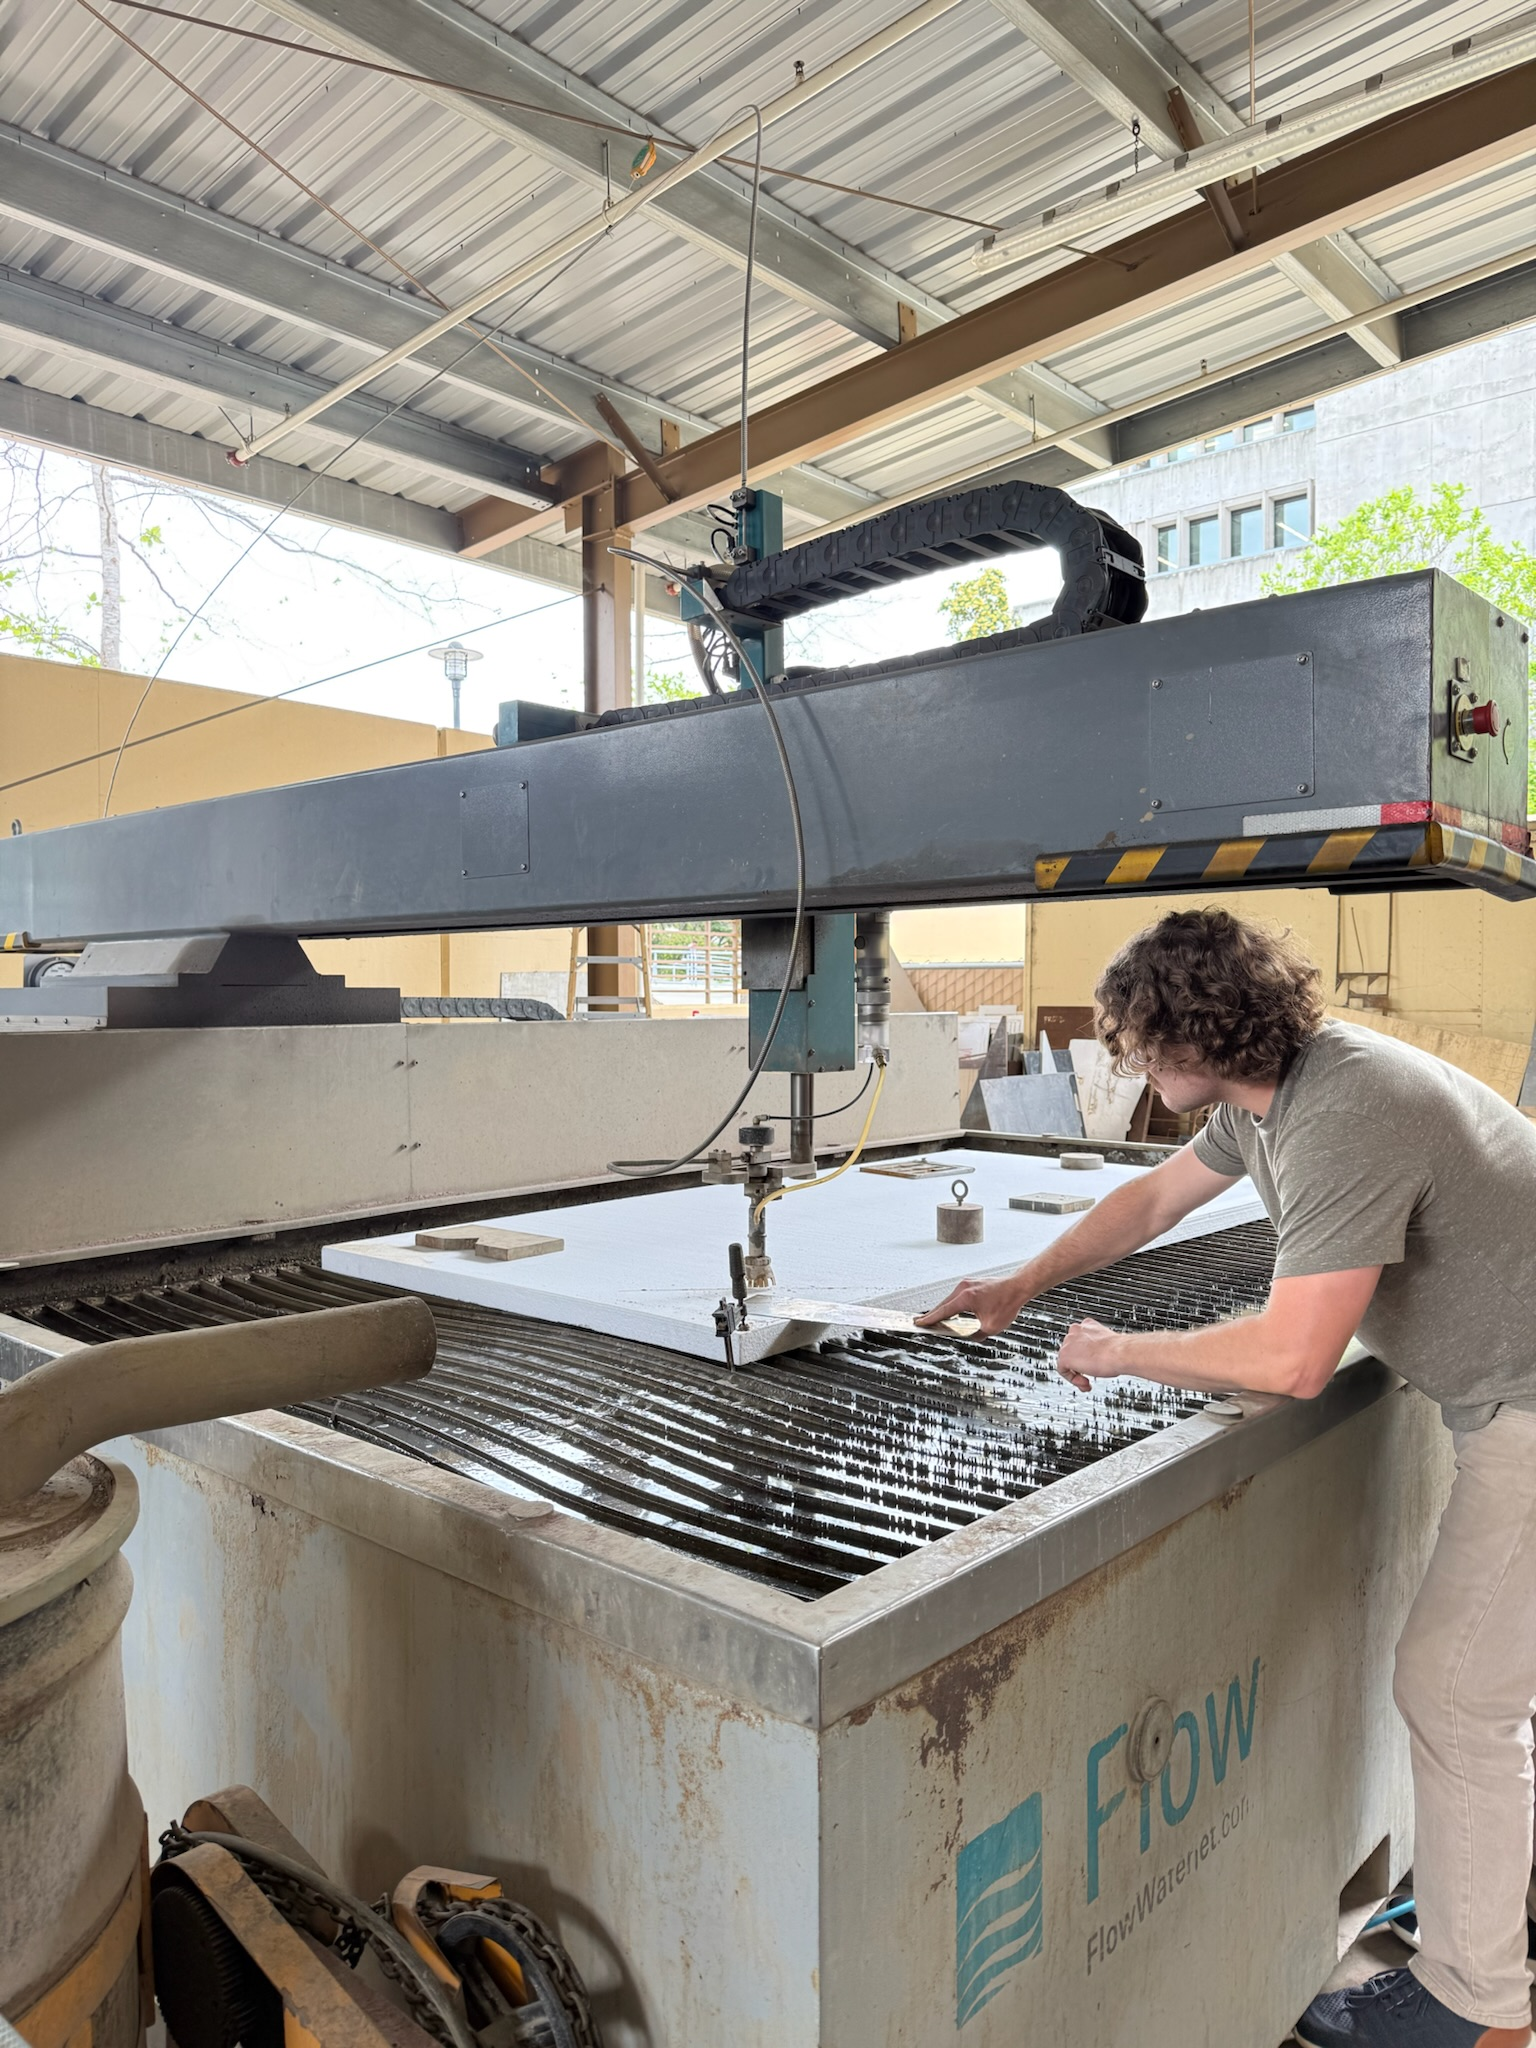
\includegraphics[
        width=3.10in,
        height=1.40in,
        keepaspectratio
    ]{waterjet_foam}
};
\draw[RuleGray,line width=0.55pt,rounded corners=4pt]
    ($(current page.north west)+(0.43in,-3.36in)$)
    rectangle
    ($(current page.north west)+(3.71in,-4.85in)$);

% Row 1 image 2
\node[anchor=center,inner sep=0pt]
at ($(current page.north west)+(5.50in,-4.105in)$)
{
    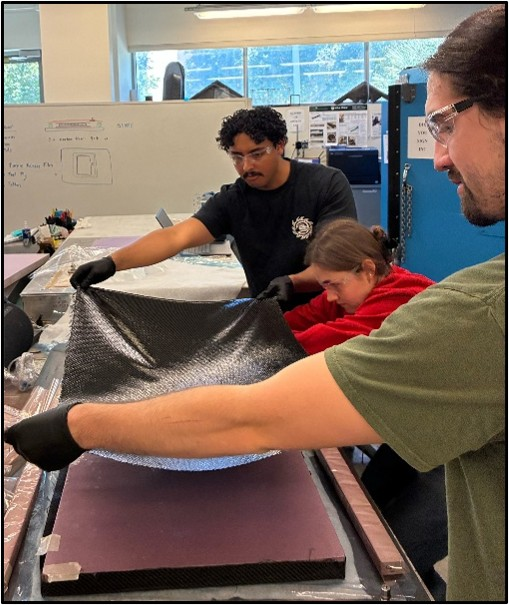
\includegraphics[
        width=3.10in,
        height=1.40in,
        keepaspectratio
    ]{group_layup}
};
\draw[RuleGray,line width=0.55pt,rounded corners=4pt]
    ($(current page.north west)+(3.86in,-3.36in)$)
    rectangle
    ($(current page.north west)+(7.14in,-4.85in)$);

% Row 1 image 3
\node[anchor=center,inner sep=0pt]
at ($(current page.north west)+(8.935in,-4.105in)$)
{
    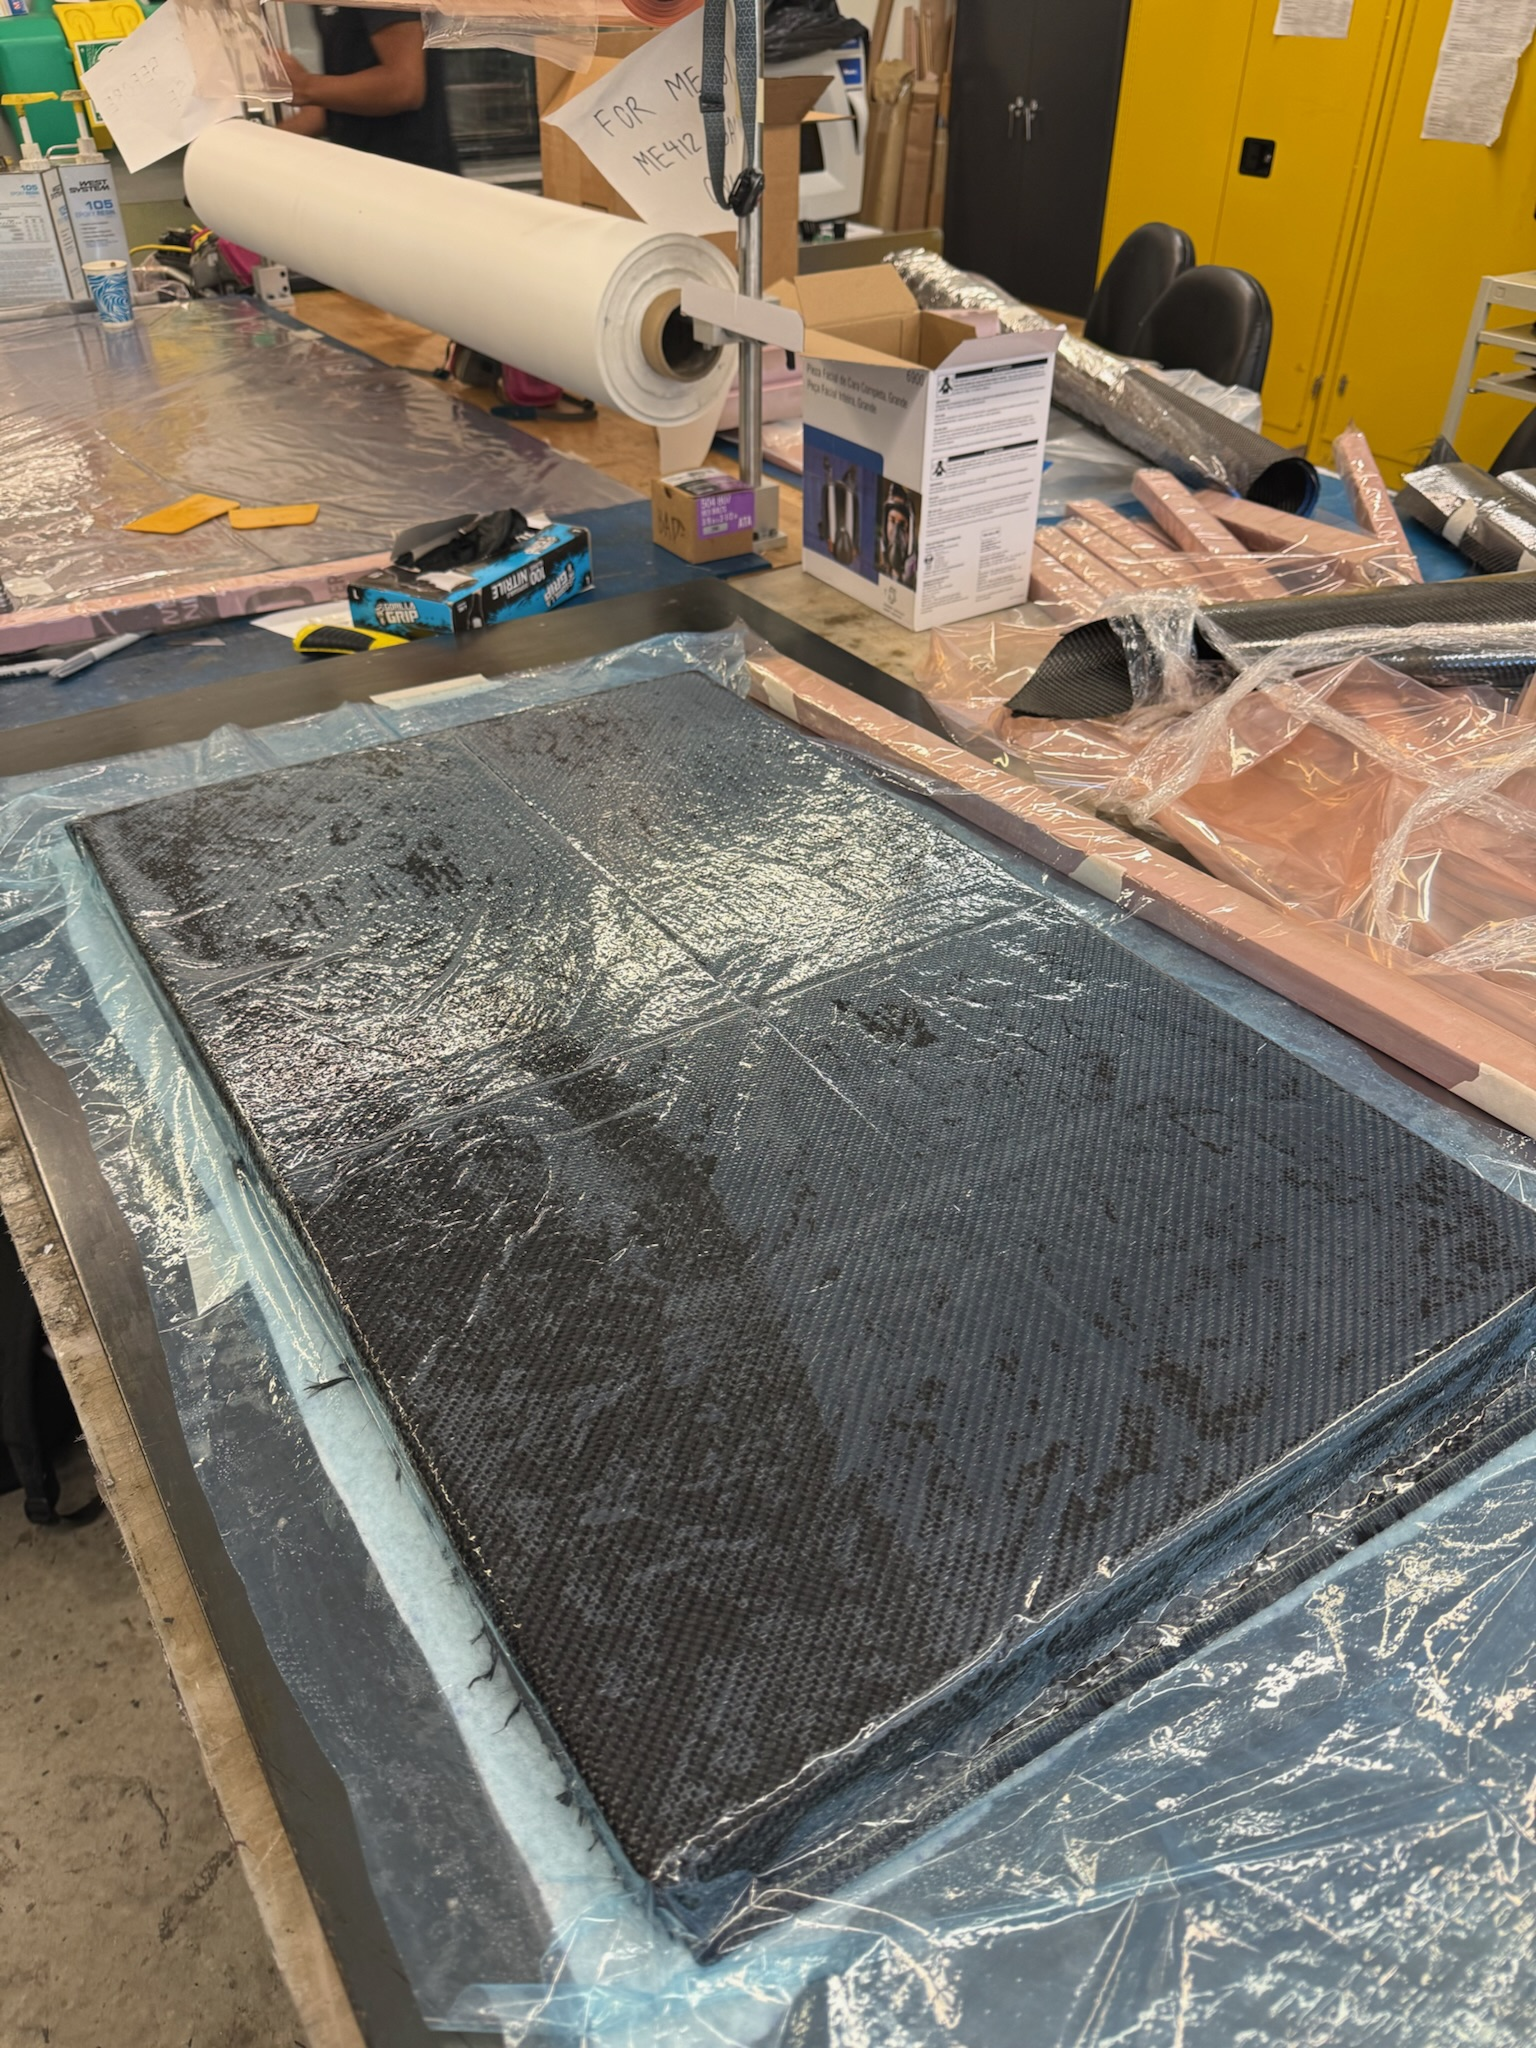
\includegraphics[
        width=3.10in,
        height=1.40in,
        keepaspectratio
    ]{blue_perforrated_film_layup}
};
\draw[RuleGray,line width=0.55pt,rounded corners=4pt]
    ($(current page.north west)+(7.29in,-3.36in)$)
    rectangle
    ($(current page.north east)+(-0.42in,-4.85in)$);

% Row 1 captions
\node[anchor=north,text=Muted,font=\sffamily\fontsize{6.7}{7.3}\selectfont]
at ($(current page.north west)+(2.07in,-4.90in)$)
{1. Waterjet-cut core and perimeter geometry};

\node[anchor=north,text=Muted,font=\sffamily\fontsize{6.7}{7.3}\selectfont]
at ($(current page.north west)+(5.50in,-4.90in)$)
{2. Team wet layup under my process guidance};

\node[anchor=north,text=Muted,font=\sffamily\fontsize{6.7}{7.3}\selectfont]
at ($(current page.north west)+(8.935in,-4.90in)$)
{3. Perforated film, breather, and vacuum enclosure};

% Row 2 image 1
\node[anchor=center,inner sep=0pt]
at ($(current page.north west)+(2.07in,-5.875in)$)
{
    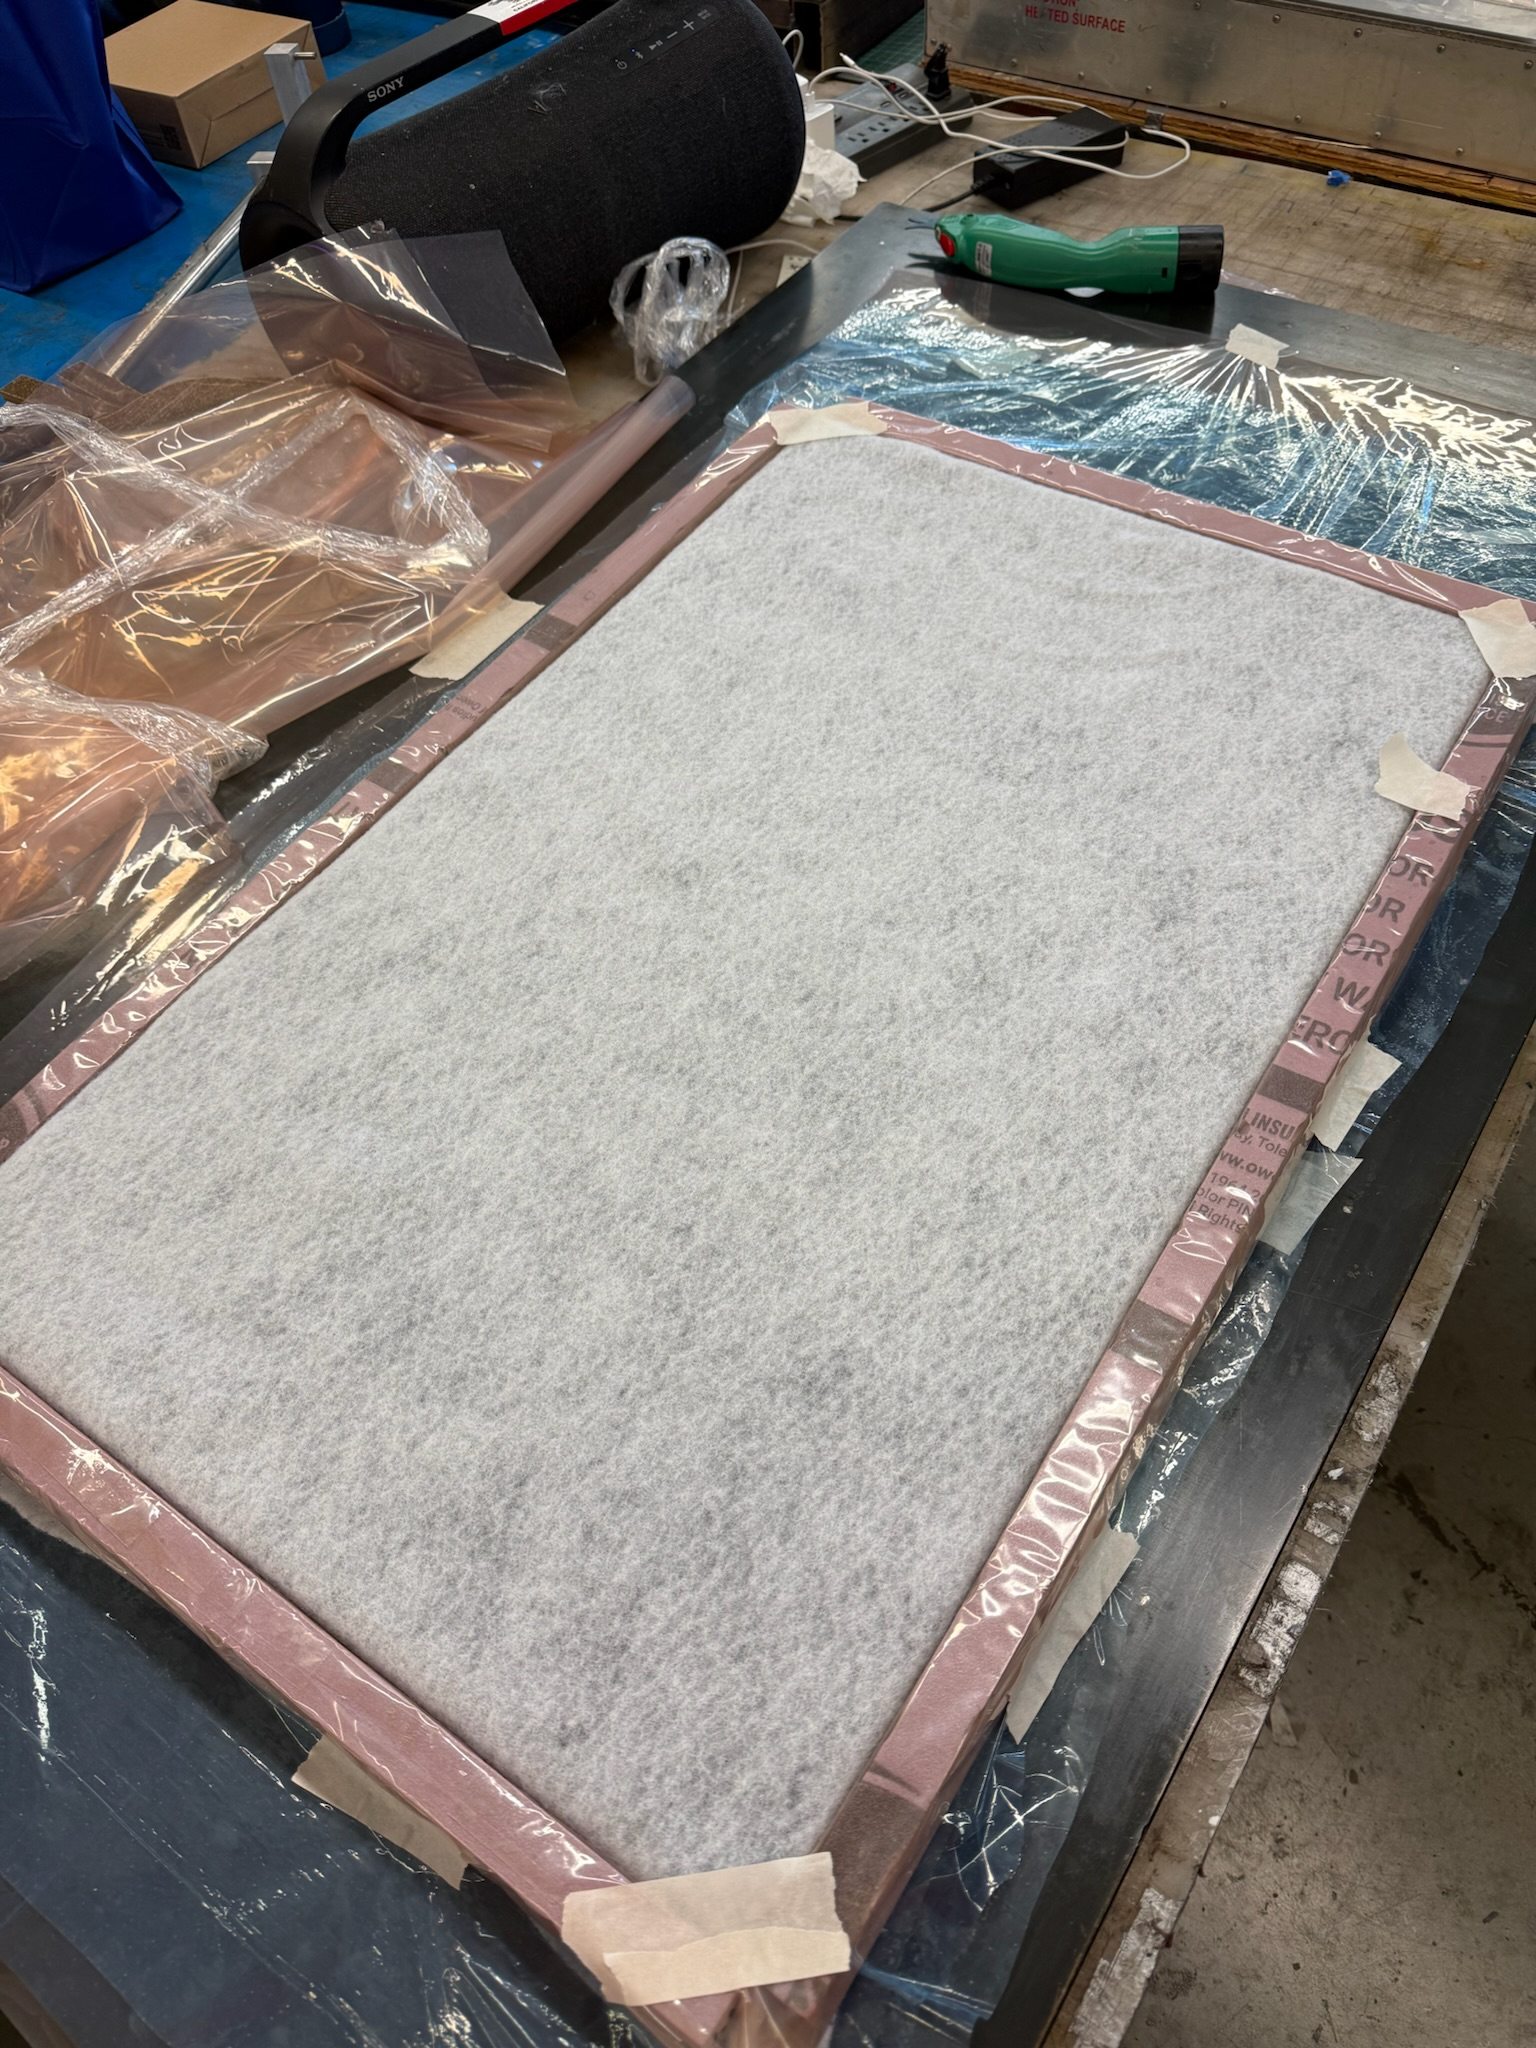
\includegraphics[
        width=3.10in,
        height=1.40in,
        keepaspectratio
    ]{completed_layup}
};
\draw[RuleGray,line width=0.55pt,rounded corners=4pt]
    ($(current page.north west)+(0.43in,-5.13in)$)
    rectangle
    ($(current page.north west)+(3.71in,-6.62in)$);

% Row 2 image 2 — oven chamber used only as a reliable vacuum enclosure; no heat applied
\node[anchor=center,inner sep=0pt]
at ($(current page.north west)+(5.50in,-5.875in)$)
{
    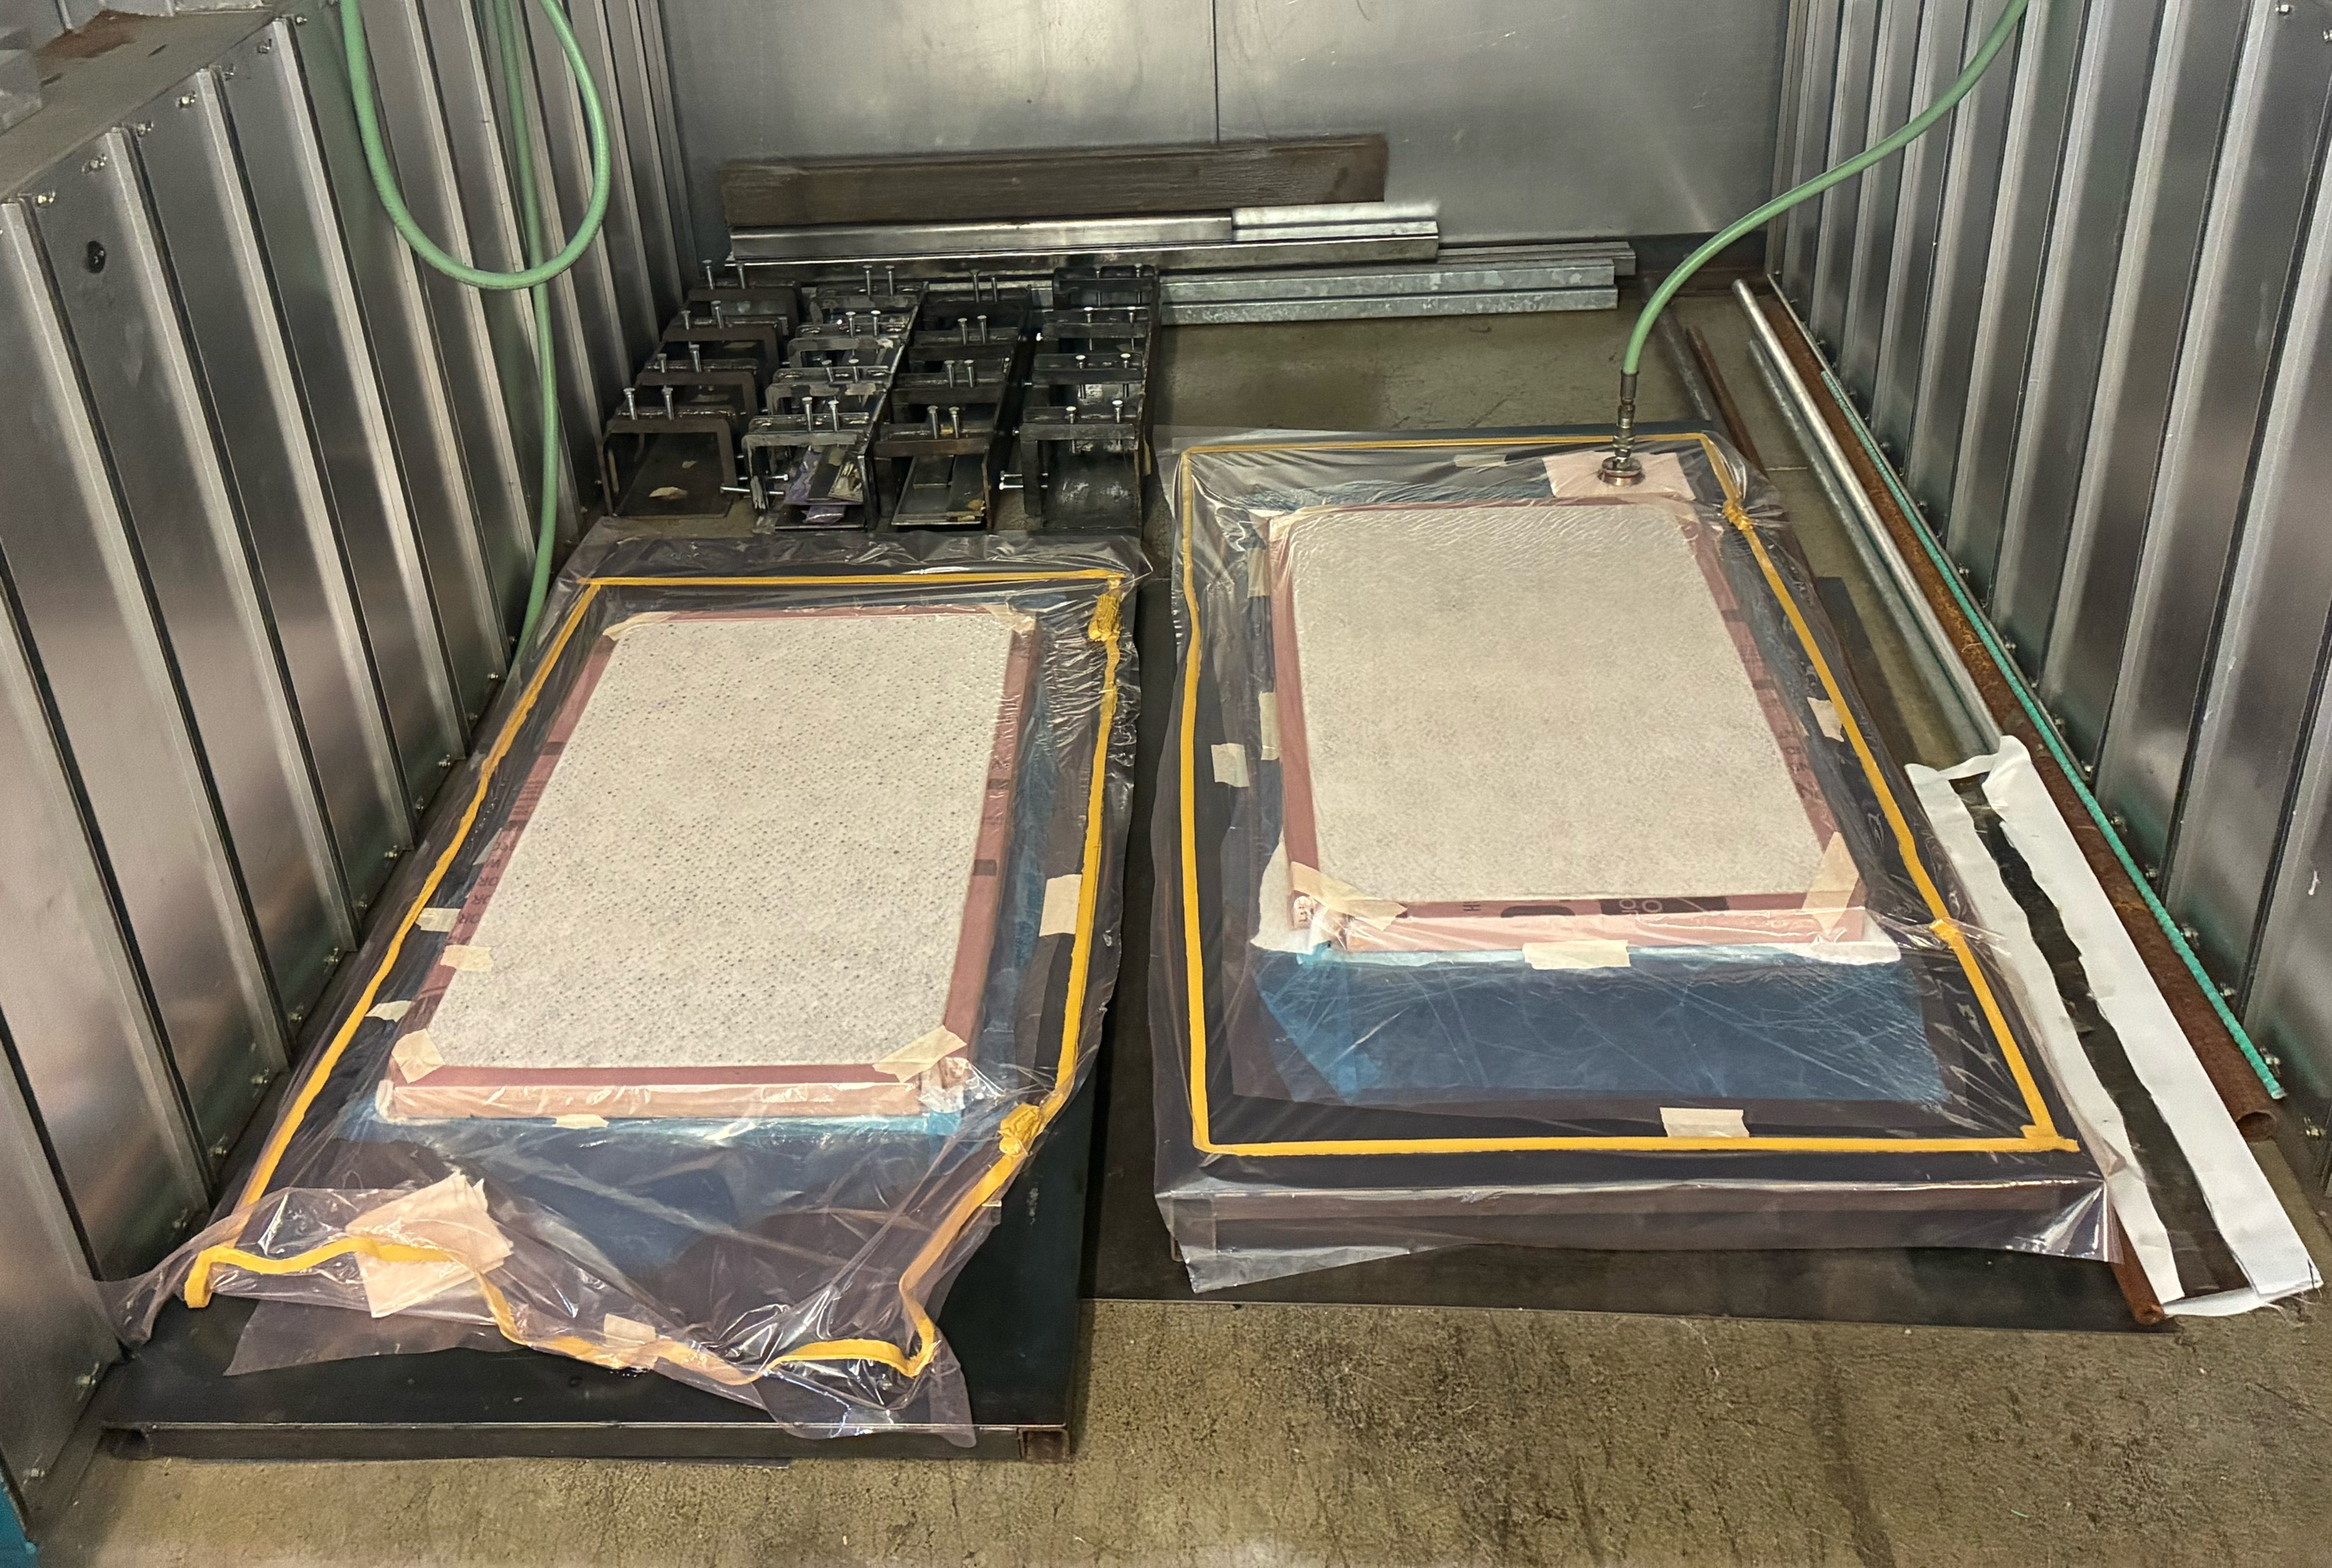
\includegraphics[
        width=3.10in,
        height=1.40in,
        keepaspectratio
    ]{layups_in_composite_oven_under_vacuumPressure}
};
\draw[RuleGray,line width=0.55pt,rounded corners=4pt]
    ($(current page.north west)+(3.86in,-5.13in)$)
    rectangle
    ($(current page.north west)+(7.14in,-6.62in)$);

% Row 2 image 3
\node[anchor=center,inner sep=0pt]
at ($(current page.north west)+(8.935in,-5.875in)$)
{
    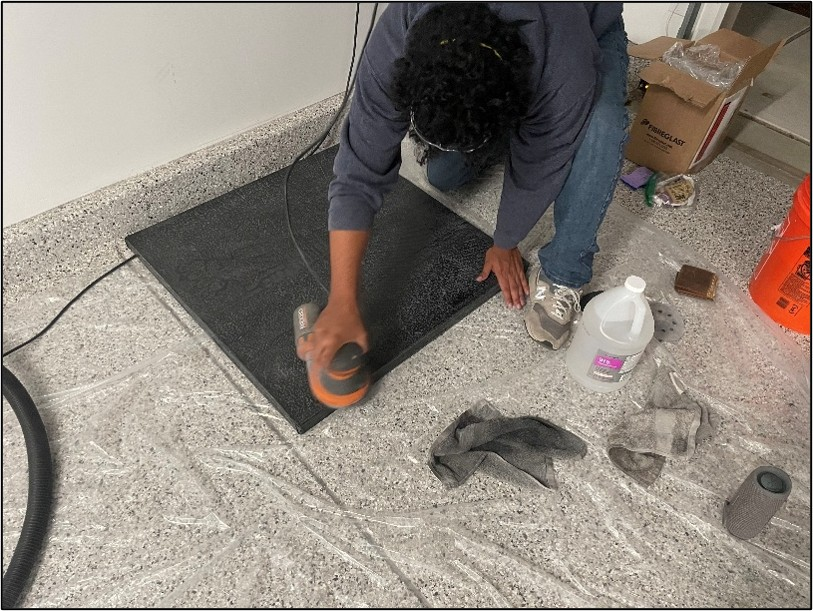
\includegraphics[
        width=3.10in,
        height=1.40in,
        keepaspectratio
    ]{garage_sanding}
};
\draw[RuleGray,line width=0.55pt,rounded corners=4pt]
    ($(current page.north west)+(7.29in,-5.13in)$)
    rectangle
    ($(current page.north east)+(-0.42in,-6.62in)$);

% Row 2 captions
\node[anchor=north,text=Muted,font=\sffamily\fontsize{6.7}{7.3}\selectfont]
at ($(current page.north west)+(2.07in,-6.67in)$)
{4. Fully saturated carbon skin and foam sandwich};

\node[anchor=north,text=Muted,font=\sffamily\fontsize{6.7}{7.3}\selectfont]
at ($(current page.north west)+(5.50in,-6.67in)$)
{5. Room-temperature cure under continuous vacuum};

\node[anchor=north,text=Muted,font=\sffamily\fontsize{6.7}{7.3}\selectfont]
at ($(current page.north west)+(8.935in,-6.67in)$)
{6. Post-processing and surface preparation};

% Bottom callouts
\fill[Panel,rounded corners=4pt]
    ($(current page.north west)+(0.43in,-6.95in)$)
    rectangle
    ($(current page.north west)+(5.48in,-7.60in)$);

\draw[RuleGray,line width=0.55pt,rounded corners=4pt]
    ($(current page.north west)+(0.43in,-6.95in)$)
    rectangle
    ($(current page.north west)+(5.48in,-7.60in)$);

\node[
    anchor=north west,
    text=DeepGreen,
    font=\sffamily\bfseries\fontsize{7.0}{7.6}\selectfont
]
at ($(current page.north west)+(0.63in,-7.08in)$)
{FROM THREE LAYUPS TO ONE};

\node[
    anchor=north west,
    align=left,
    text width=4.56in,
    text=Ink,
    font=\fontsize{6.45}{7.45}\selectfont
]
at ($(current page.north west)+(0.63in,-7.29in)$)
{
The Envelope Method reduced labor, cure cycles, handling,
alignment risk, and time spent forming numerous vacuum-bag
pleats around the 1.5-inch-thick XPS panels.
};

\fill[Panel,rounded corners=4pt]
    ($(current page.north west)+(5.68in,-6.95in)$)
    rectangle
    ($(current page.north east)+(-0.42in,-7.60in)$);

\draw[RuleGray,line width=0.55pt,rounded corners=4pt]
    ($(current page.north west)+(5.68in,-6.95in)$)
    rectangle
    ($(current page.north east)+(-0.42in,-7.60in)$);

\node[
    anchor=north west,
    text=DeepGreen,
    font=\sffamily\bfseries\fontsize{7.0}{7.6}\selectfont
]
at ($(current page.north west)+(5.88in,-7.08in)$)
{WHY SURFACE-BONDED HARDWARE};

\node[
    anchor=north west,
    align=left,
    text width=4.55in,
    text=Ink,
    font=\fontsize{6.45}{7.45}\selectfont
]
at ($(current page.north west)+(5.88in,-7.29in)$)
{
Adhesively bonded hinges and fixtures preserved the clean
composite exterior and avoided drilled inserts, foam-core
crushing, added stress concentrations, and new leak paths.
};


% Footer
\node[
    anchor=south west,
    text=white,
    font=\sffamily\bfseries\fontsize{7.1}{7.7}\selectfont
]
at ($(current page.south west)+(0.42in,0.17in)$)
{\faArrowLeft\ PRODUCT ARCHITECTURE};

\node[
    anchor=south,
    text=white,
    font=\sffamily\fontsize{7.0}{7.6}\selectfont
]
at ($(current page.south)+(0,0.17in)$)
{TORO COVER \hspace{6pt} 2 / 3};

\node[
    anchor=south east,
    text=white,
    font=\sffamily\bfseries\fontsize{7.1}{7.7}\selectfont
]
at ($(current page.south east)+(-0.42in,0.17in)$)
{VALIDATION \& TAKEAWAYS \faArrowRight};

\end{tikzpicture}


% ============================================================
% PAGE 3 — FINISHING, VALIDATION, AND TAKEAWAYS
% ============================================================

\clearpage
\thispagestyle{empty}
\hypertarget{toro-results}{}
\null

\begin{tikzpicture}[remember picture,overlay]

% Background and bars
\fill[white]
    (current page.south west)
    rectangle
    (current page.north east);

\fill[DeepGreen]
    (current page.north west)
    rectangle
    ($(current page.north east)+(0,-0.095in)$);

\fill[PolyGold]
    ($(current page.north west)+(0,-0.095in)$)
    rectangle
    ($(current page.north east)+(0,-0.14in)$);

\fill[DeepGreen]
    (current page.south west)
    rectangle
    ($(current page.south east)+(0,0.36in)$);

\fill[PolyGold]
    ($(current page.south west)+(0,0.36in)$)
    rectangle
    ($(current page.south east)+(0,0.405in)$);

% Header
\node[
    anchor=north west,
    text=PolyGold,
    font=\sffamily\bfseries\fontsize{8.1}{8.7}\selectfont
]
at ($(current page.north west)+(0.42in,-0.39in)$)
{TORO COVER \hspace{5pt}/\hspace{5pt} VALIDATION AND ENGINEERING TAKEAWAYS};

\node[
    anchor=north west,
    text=DeepGreen,
    font=\bfseries\fontsize{22.5}{23.5}\selectfont
]
at ($(current page.north west)+(0.40in,-0.67in)$)
{FROM PROTOTYPE TO PRODUCT PATHWAY};

\node[
    anchor=north west,
    text=Muted,
    font=\sffamily\fontsize{8.7}{9.6}\selectfont
]
at ($(current page.north west)+(0.42in,-1.12in)$)
{Environmental protection, usability testing, scope decisions, and lessons from technical leadership};

\fill[PolyGold]
    ($(current page.north west)+(0.42in,-1.36in)$)
    rectangle
    ($(current page.north west)+(5.8in,-1.315in)$);

% Finishing title
\node[
    anchor=north west,
    text=DeepGreen,
    font=\sffamily\bfseries\fontsize{8.0}{8.7}\selectfont
]
at ($(current page.north west)+(0.43in,-1.62in)$)
{OUTDOOR FINISHING AND ENVIRONMENTAL PROTECTION};

% Image 1
\node[anchor=center,inner sep=0pt]
at ($(current page.north west)+(1.705in,-2.655in)$)
{
    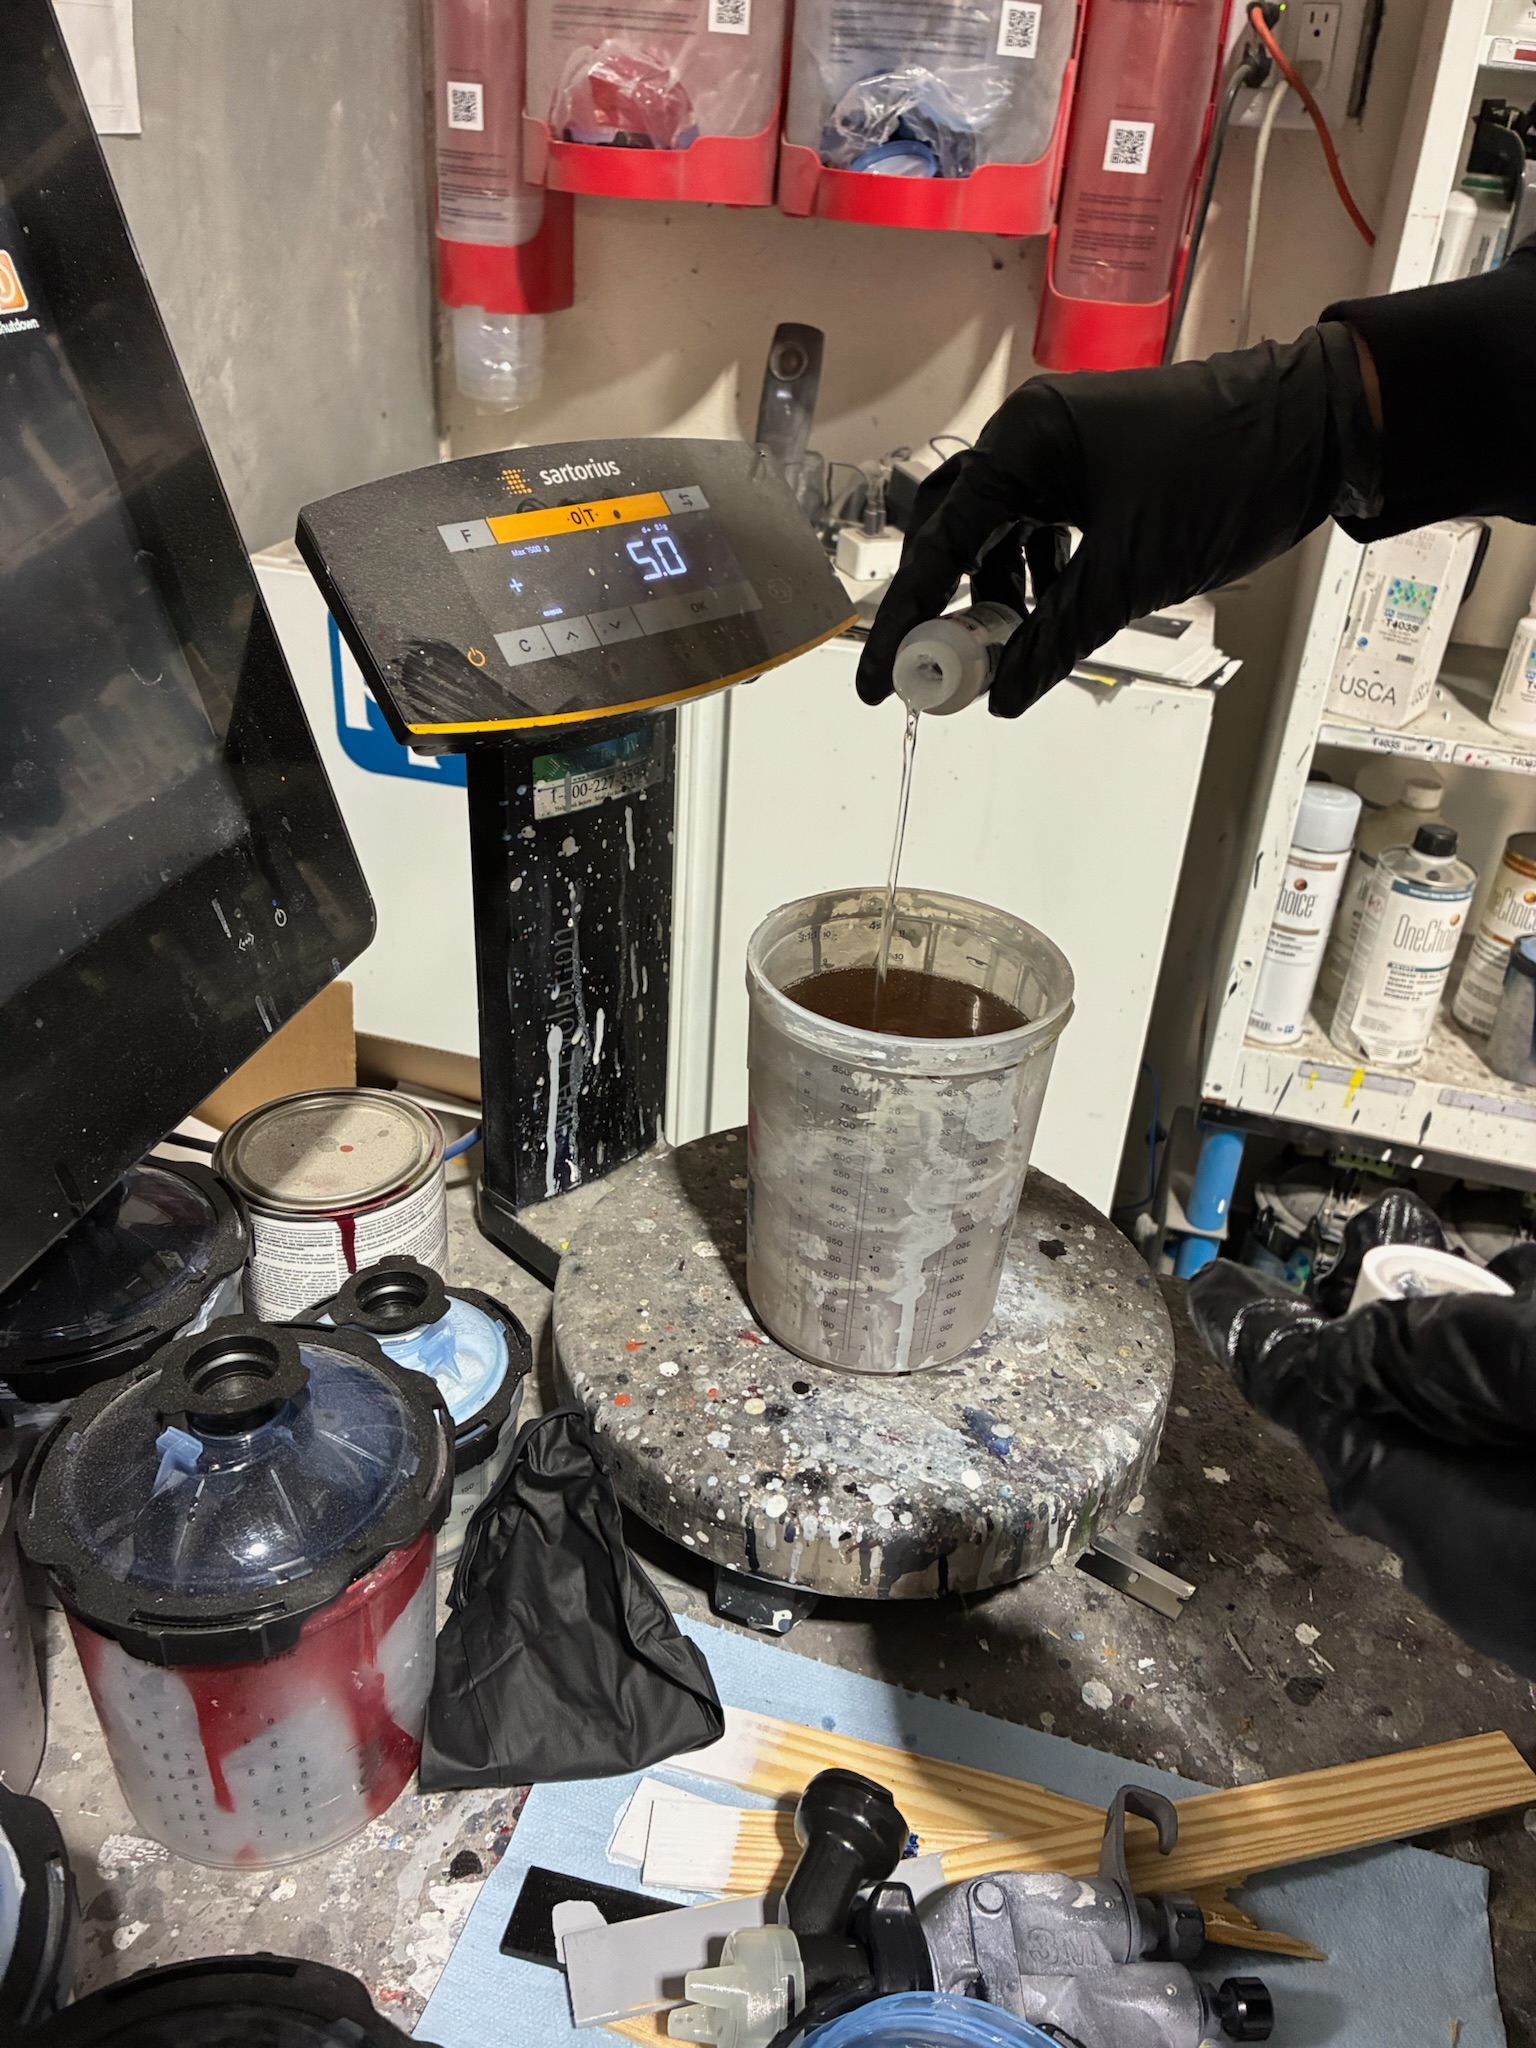
\includegraphics[
        width=2.35in,
        height=1.40in,
        keepaspectratio
    ]{spray_topcoat_prep}
};
\draw[RuleGray,line width=0.55pt,rounded corners=4pt]
    ($(current page.north west)+(0.43in,-1.91in)$)
    rectangle
    ($(current page.north west)+(2.98in,-3.40in)$);

% Image 2
\node[anchor=center,inner sep=0pt]
at ($(current page.north west)+(4.375in,-2.655in)$)
{
    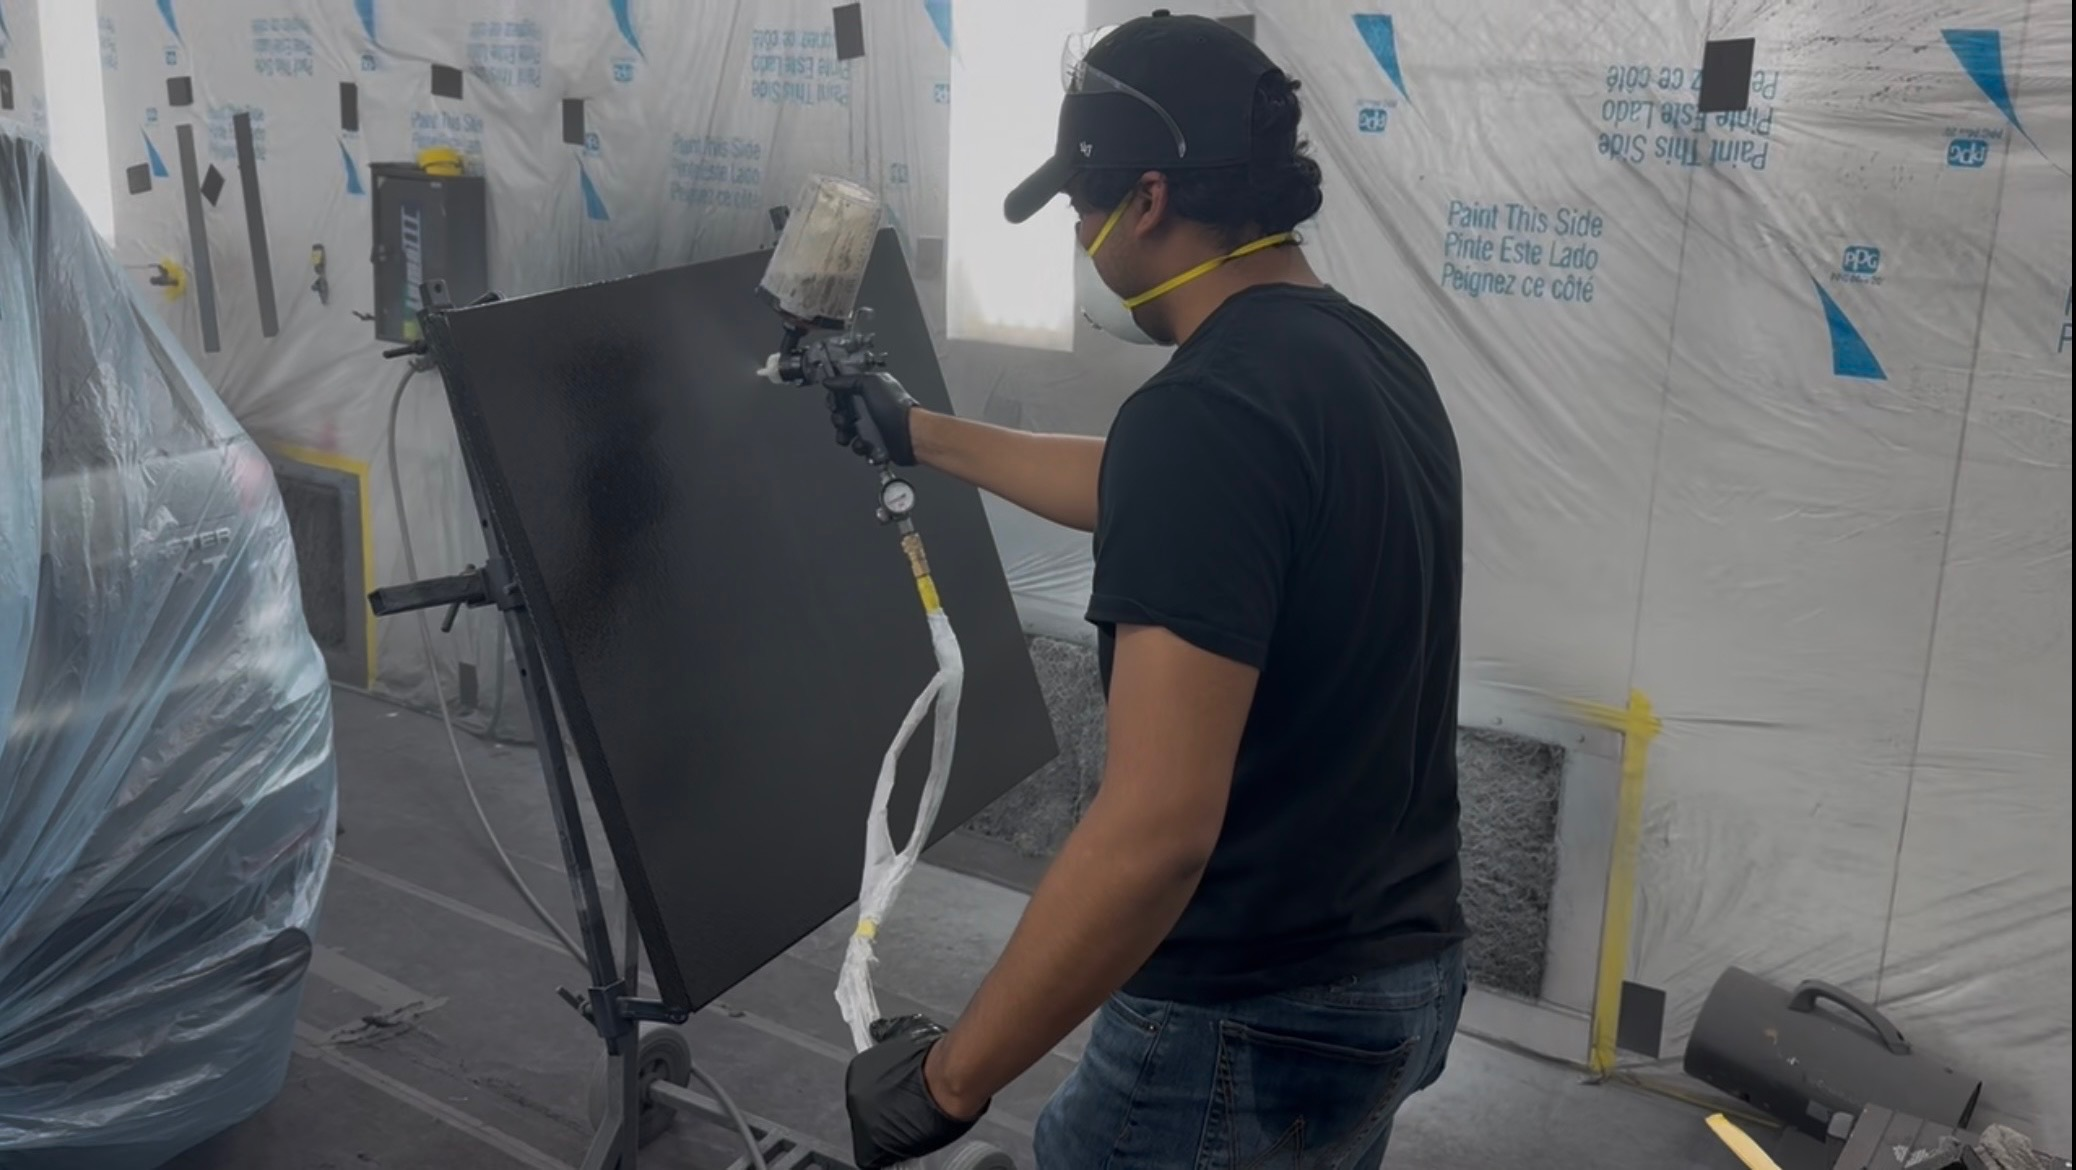
\includegraphics[
        width=2.35in,
        height=1.40in,
        keepaspectratio
    ]{spraying_topcoat}
};
\draw[RuleGray,line width=0.55pt,rounded corners=4pt]
    ($(current page.north west)+(3.10in,-1.91in)$)
    rectangle
    ($(current page.north west)+(5.65in,-3.40in)$);

% Image 3
\node[anchor=center,inner sep=0pt]
at ($(current page.north west)+(7.045in,-2.655in)$)
{
    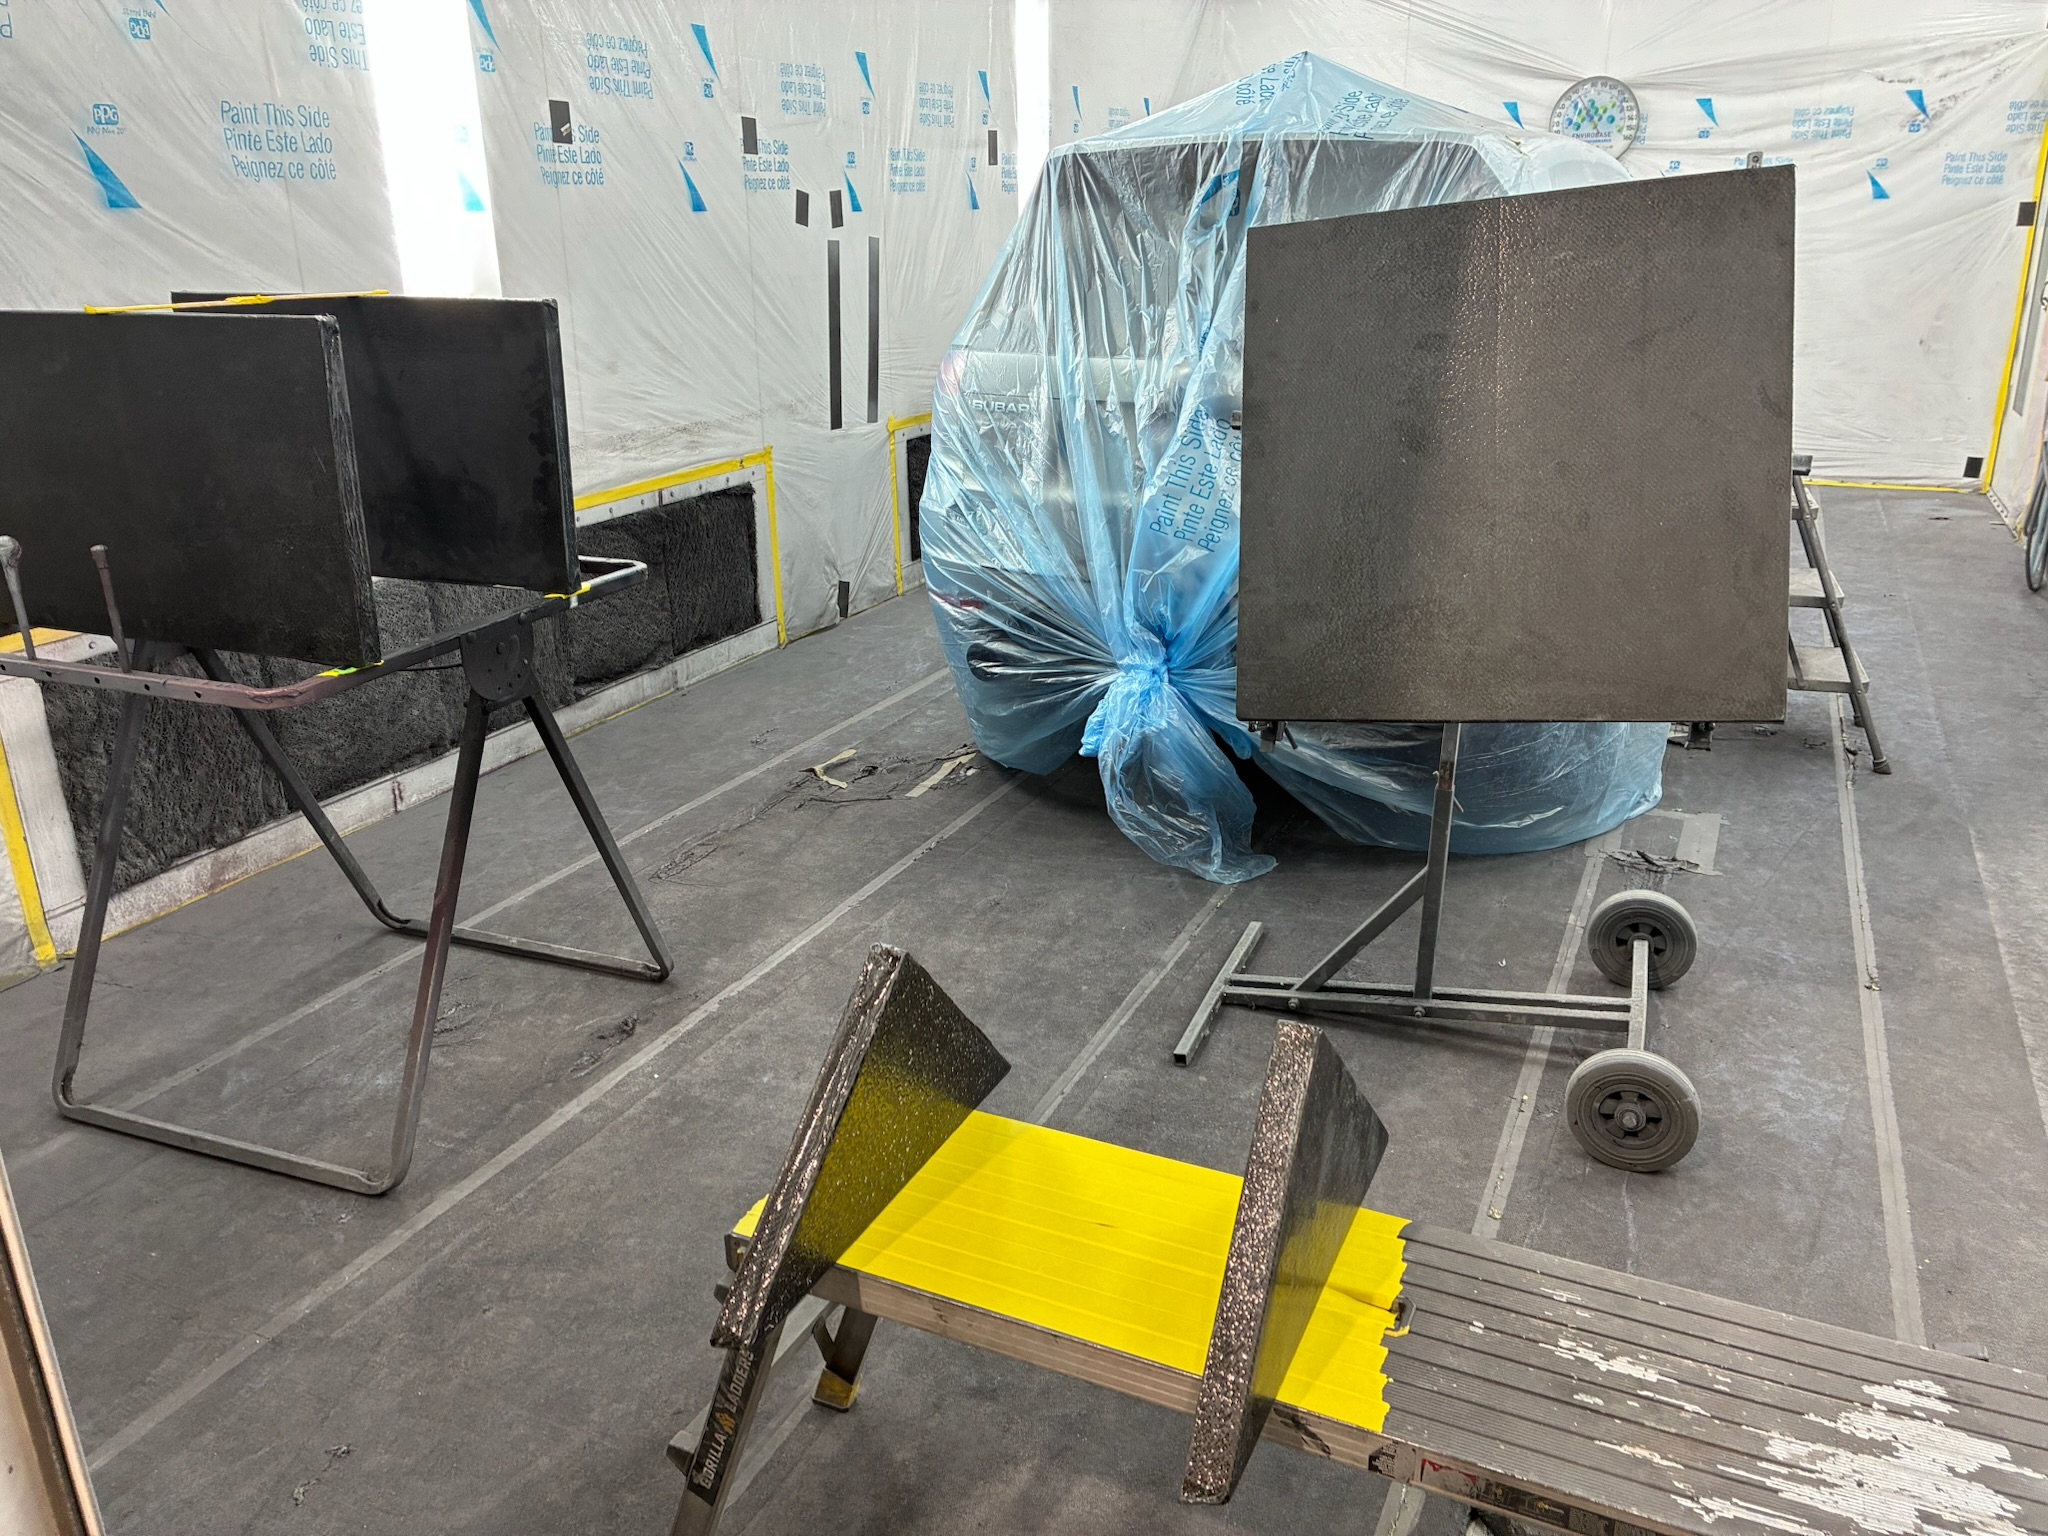
\includegraphics[
        width=2.35in,
        height=1.40in,
        keepaspectratio
    ]{topcoat_setup_apparatus}
};
\draw[RuleGray,line width=0.55pt,rounded corners=4pt]
    ($(current page.north west)+(5.77in,-1.91in)$)
    rectangle
    ($(current page.north west)+(8.32in,-3.40in)$);

% Image 4
\node[anchor=center,inner sep=0pt]
at ($(current page.north west)+(9.50in,-2.655in)$)
{
    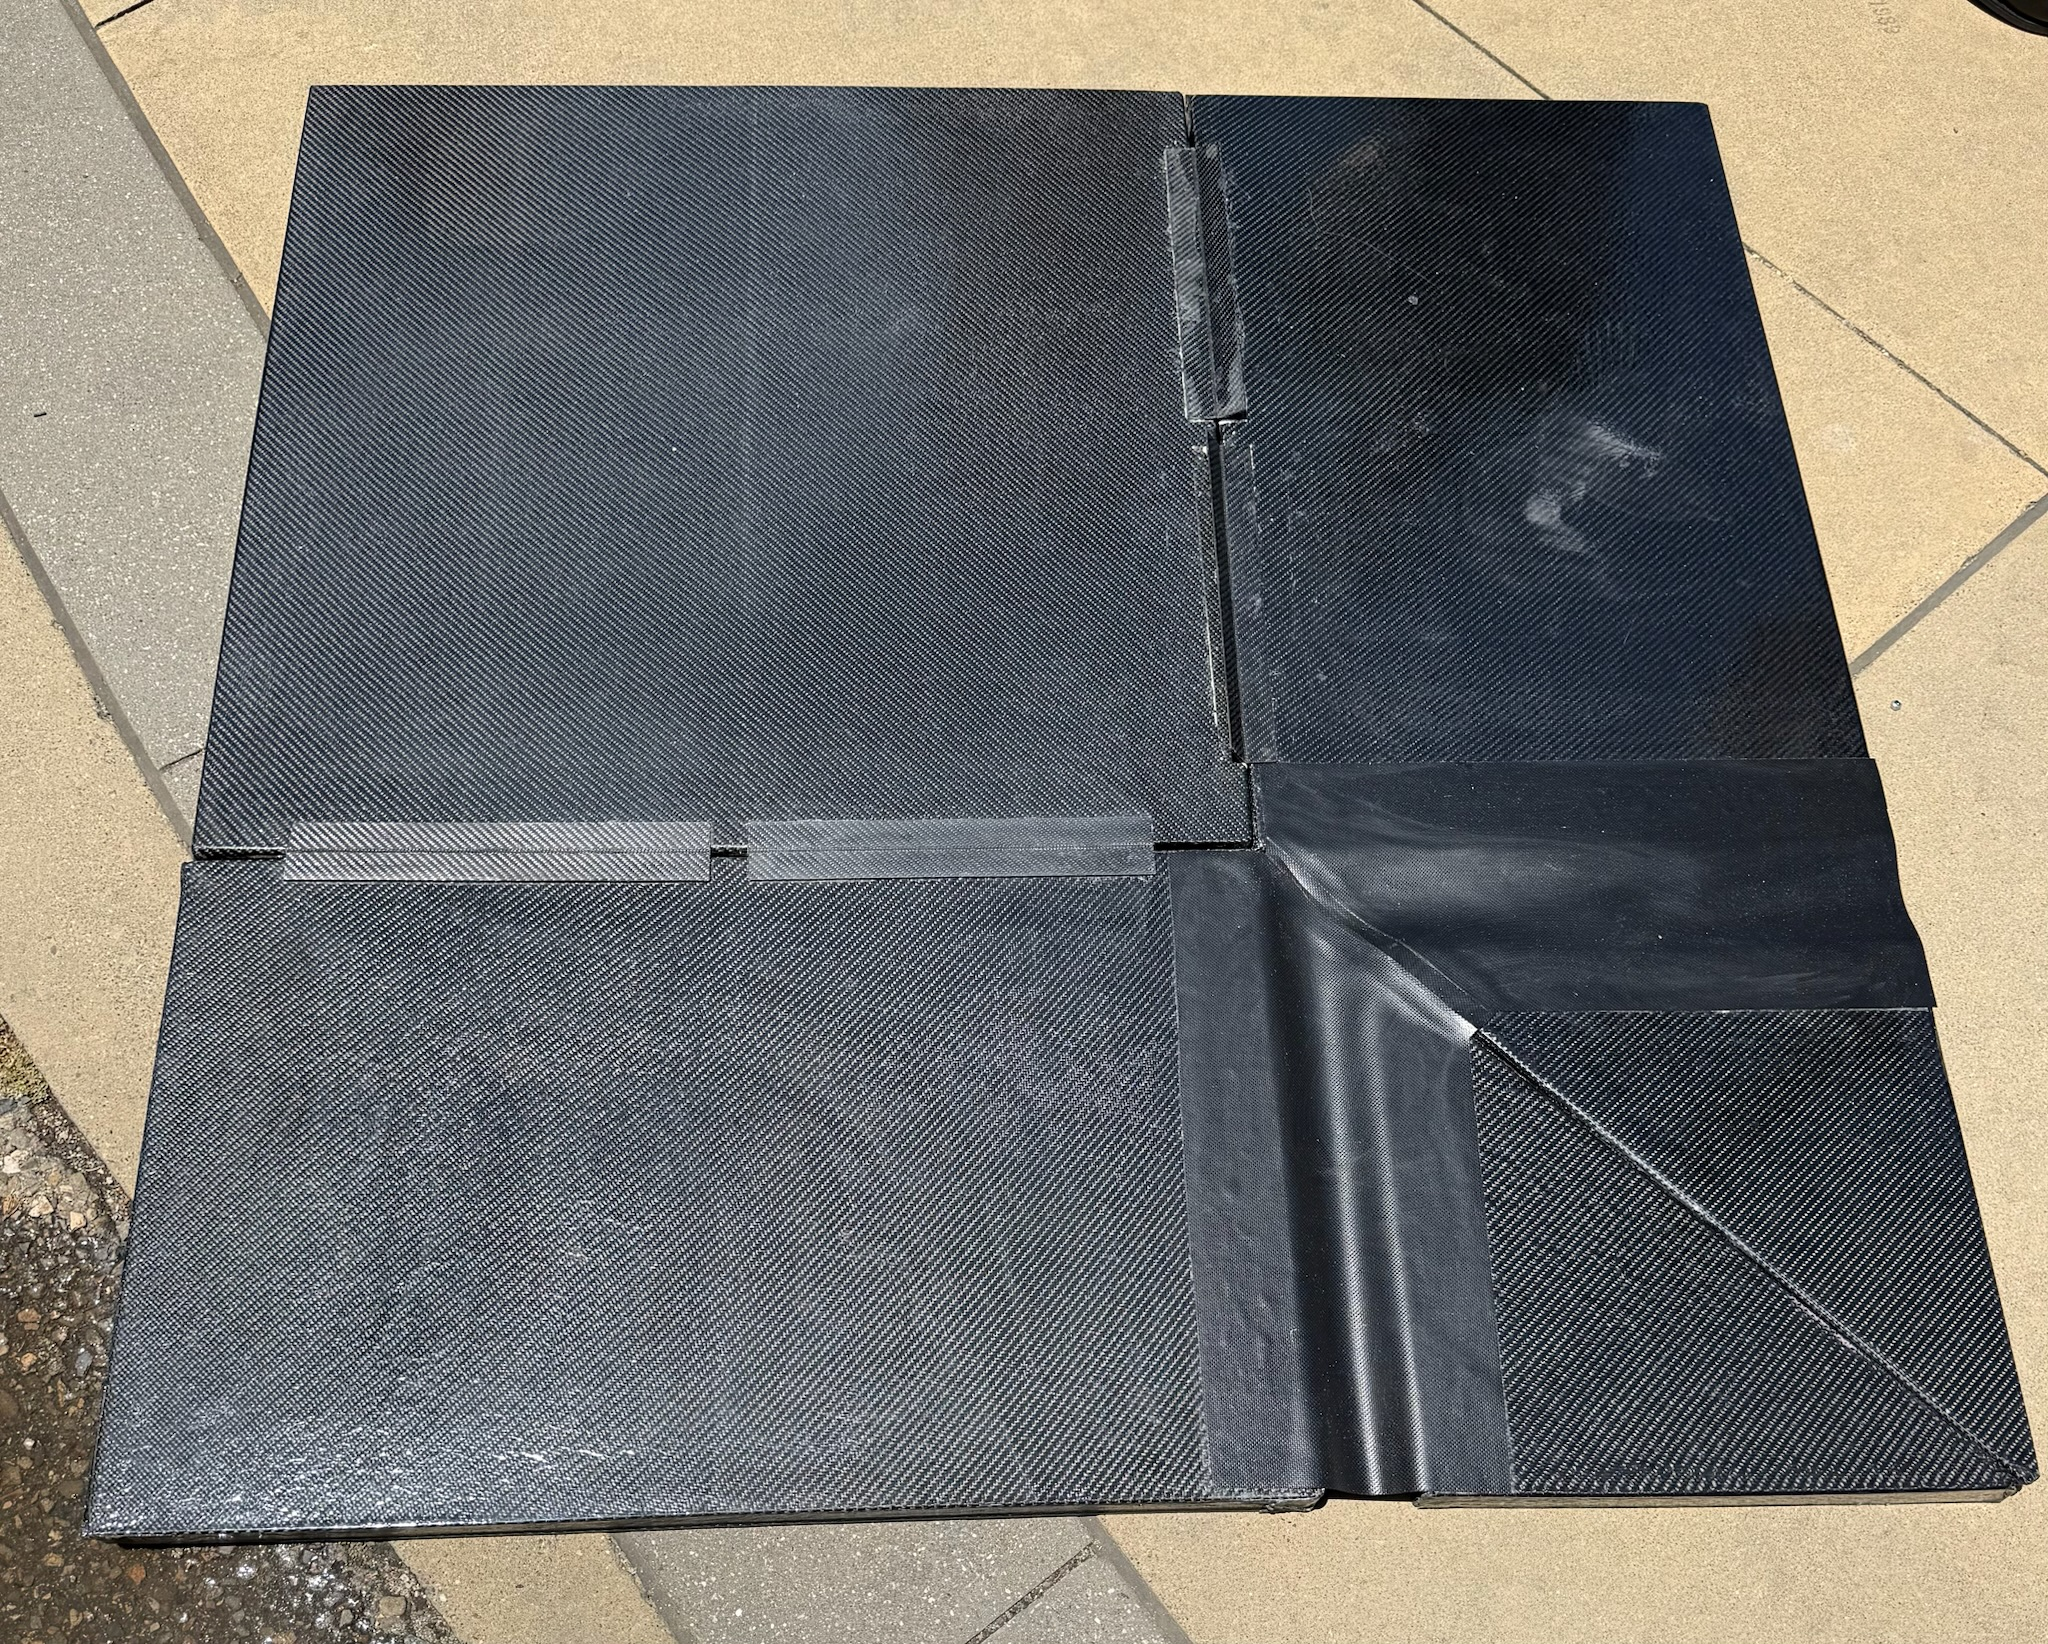
\includegraphics[
        width=2.35in,
        height=1.40in,
        keepaspectratio
    ]{refined_final_toro_cover_partial_carbon_model}
};
\draw[RuleGray,line width=0.55pt,rounded corners=4pt]
    ($(current page.north west)+(8.44in,-1.91in)$)
    rectangle
    ($(current page.north east)+(-0.42in,-3.40in)$);

% Captions
\node[anchor=north,text=Muted,font=\sffamily\fontsize{6.7}{7.3}\selectfont]
at ($(current page.north west)+(1.705in,-3.45in)$)
{Topcoat material preparation};

\node[anchor=north,text=Muted,font=\sffamily\fontsize{6.7}{7.3}\selectfont]
at ($(current page.north west)+(4.375in,-3.45in)$)
{Automotive-booth topcoat application};

\node[anchor=north,text=Muted,font=\sffamily\fontsize{6.7}{7.3}\selectfont]
at ($(current page.north west)+(7.045in,-3.45in)$)
{Coated panels drying after application};

\node[anchor=north,text=Muted,font=\sffamily\fontsize{6.7}{7.3}\selectfont]
at ($(current page.north west)+(9.50in,-3.45in)$)
{Partial carbon manufacturing model};

% Environmental rationale
\fill[SoftGold,rounded corners=4pt]
    ($(current page.north west)+(0.43in,-3.73in)$)
    rectangle
    ($(current page.north east)+(-0.42in,-4.76in)$);

\node[
    anchor=north west,
    align=left,
    text width=9.75in,
    text=Ink,
    font=\fontsize{7.05}{8.25}\selectfont
]
at ($(current page.north west)+(0.65in,-3.89in)$)
{
Because the sponsor required a carbon-fiber cover for outdoor use near chlorinated water,
environmental protection became a functional requirement rather than a cosmetic finish.
I selected and personally sprayed a UV-resistant Sunshield topcoat to seal minor laminate
porosity, reduce moisture ingress, preserve the carbon appearance, limit UV degradation of
the epoxy matrix, and isolate the composite surface from nearby metallic hardware.
};

% Results title
\node[
    anchor=north west,
    text=DeepGreen,
    font=\sffamily\bfseries\fontsize{8.0}{8.7}\selectfont
]
at ($(current page.north west)+(0.43in,-4.94in)$)
{FUNCTIONAL PROTOTYPE RESULTS};

% ------------------------------------------------------------
% Matched lower panels — larger type and improved allocation
% ------------------------------------------------------------

% Left results panel
\fill[SoftGreen,rounded corners=5pt]
    ($(current page.north west)+(0.43in,-5.22in)$)
    rectangle
    ($(current page.north west)+(5.98in,-7.39in)$);

\draw[RuleGray,line width=0.65pt,rounded corners=5pt]
    ($(current page.north west)+(0.43in,-5.22in)$)
    rectangle
    ($(current page.north west)+(5.98in,-7.39in)$);

\fill[DeepGreen,rounded corners=5pt]
    ($(current page.north west)+(0.43in,-5.22in)$)
    rectangle
    ($(current page.north west)+(5.98in,-5.58in)$);

\fill[DeepGreen]
    ($(current page.north west)+(0.43in,-5.40in)$)
    rectangle
    ($(current page.north west)+(5.98in,-5.58in)$);

\node[anchor=west,text=white,
      font=\sffamily\bfseries\fontsize{7.0}{7.6}\selectfont]
at ($(current page.north west)+(0.66in,-5.40in)$)
{SPECIFICATION};

\node[anchor=west,text=white,
      font=\sffamily\bfseries\fontsize{7.0}{7.6}\selectfont]
at ($(current page.north west)+(3.02in,-5.40in)$)
{RESULT};

\node[anchor=east,text=white,
      font=\sffamily\bfseries\fontsize{7.0}{7.6}\selectfont]
at ($(current page.north west)+(5.55in,-5.40in)$)
{STATUS};

\node[
    anchor=north west,
    align=left,
    text width=2.15in,
    text=Ink,
    font=\bfseries\fontsize{7.15}{8.55}\selectfont
]
at ($(current page.north west)+(0.66in,-5.72in)$)
{
Deployment time\\[3.4pt]
Removal time\\[3.4pt]
Single-user operation\\[3.4pt]
Single-side operation\\[3.4pt]
Deployment steps\\[3.4pt]
Removal steps\\[3.4pt]
Weight\\[3.4pt]
Folded storage
};

\node[
    anchor=north west,
    align=left,
    text width=1.45in,
    text=Ink,
    font=\fontsize{7.15}{8.55}\selectfont
]
at ($(current page.north west)+(3.02in,-5.72in)$)
{
25.51 seconds\\[3.4pt]
37.22 seconds\\[3.4pt]
100\% successful\\[3.4pt]
75\% successful\\[3.4pt]
6.4 average\\[3.4pt]
9 average\\[3.4pt]
17 lb\\[3.4pt]
2.9' x 2.9' x 1.7'
};

\node[
    anchor=north east,
    align=right,
    text width=1.05in,
    text=DeepGreen,
    font=\sffamily\bfseries\fontsize{7.05}{8.55}\selectfont
]
at ($(current page.north west)+(5.55in,-5.72in)$)
{
PASS\\[3.4pt]
PASS\\[3.4pt]
PASS\\[3.4pt]
NEAR TARGET\\[3.4pt]
PASS\\[3.4pt]
PASS\\[3.4pt]
NEAR TARGET\\[3.4pt]
PASS
};

% Right takeaways panel — widened for easier reading
\fill[SoftGreen,rounded corners=5pt]
    ($(current page.north west)+(6.14in,-5.22in)$)
    rectangle
    ($(current page.north east)+(-0.42in,-7.39in)$);

\draw[RuleGray,line width=0.65pt,rounded corners=5pt]
    ($(current page.north west)+(6.14in,-5.22in)$)
    rectangle
    ($(current page.north east)+(-0.42in,-7.39in)$);

\fill[DeepGreen,rounded corners=5pt]
    ($(current page.north west)+(6.14in,-5.22in)$)
    rectangle
    ($(current page.north east)+(-0.42in,-5.58in)$);

\fill[DeepGreen]
    ($(current page.north west)+(6.14in,-5.40in)$)
    rectangle
    ($(current page.north east)+(-0.42in,-5.58in)$);

\node[anchor=west,text=white,
      font=\sffamily\bfseries\fontsize{7.1}{7.7}\selectfont]
at ($(current page.north west)+(6.38in,-5.40in)$)
{ENGINEERING TAKEAWAYS};

\node[
    anchor=north west,
    align=left,
    text width=4.02in,
    text=Ink,
    font=\fontsize{6.75}{7.85}\selectfont
]
at ($(current page.north west)+(6.38in,-5.72in)$)
{
\textbf{Manufacturing first.}
Composite manufacturing constraints should guide the product architecture from the beginning.\\[4.5pt]
\textbf{Prioritize deliberately.}
Competing requirements must be balanced intentionally instead of maximizing every objective.\\[4.5pt]
\textbf{Lead through the process.}
Clear procedures, calm communication, and respect for teammates' strengths were essential during fabrication.\\[4.5pt]
\textbf{Next iteration.}
Reduce weight, refine the fabric-hinge fold lines, and improve panel-edge clearance.
};

% Compact concluding pathway
\node[
    anchor=center,
    align=center,
    text=PolyGold,
    font=\sffamily\bfseries\fontsize{6.3}{6.9}\selectfont
]
at ($(current page.north)+(3.06in,-7.18in)$)
{PROTOTYPE \faArrowRight\ DESIGN REFINEMENT
\faArrowRight\ REPEATABLE MANUFACTURING
\faArrowRight\ PRODUCT};

% Validation resources
\node[
    anchor=north,
    align=center,
    text=DeepGreen,
    font=\sffamily\bfseries\fontsize{6.6}{7.2}\selectfont
]
at ($(current page.north)+(0,-7.58in)$)
{\href{\ToroDeploymentLink}{\faPlayCircle\ DEPLOYMENT}
\hspace{18pt}
\href{\ToroRemovalLink}{\faPlayCircle\ REMOVAL / FOLDING}
\hspace{18pt}
\href{\ToroPosterLink}{\faFilePdf\ EXPO POSTER}
\hspace{18pt}
\href{\ToroReportLink}{\faFilePdf\ FINAL REPORT}};

% Footer
\node[
    anchor=south west,
    text=white,
    font=\sffamily\bfseries\fontsize{7.1}{7.7}\selectfont
]
at ($(current page.south west)+(0.42in,0.17in)$)
{\faArrowLeft\ MANUFACTURING-DRIVEN DESIGN};

\node[
    anchor=south,
    text=white,
    font=\sffamily\fontsize{7.0}{7.6}\selectfont
]
at ($(current page.south)+(0,0.17in)$)
{TORO COVER \hspace{6pt} 3 / 3};

\node[
    anchor=south east,
    text=white,
    font=\sffamily\bfseries\fontsize{7.1}{7.7}\selectfont
]
at ($(current page.south east)+(-0.42in,0.17in)$)
{NEXT PROJECT \faArrowRight};

\end{tikzpicture}
\input{paddle}
\clearpage
 before \end{document}.
% 3. Image references use the original Overleaf base filenames
%    without extensions.
% ============================================================



% ============================================================
% CLICKABLE PROJECT RESOURCES
% All links use the exact Google Drive resources supplied.
% ============================================================
\providecommand{\ToroDrawingLink}{https://drive.google.com/file/d/1A7-7wMnRNLuQDaTgxeuUCBsGNqyXzOGV/view?usp=sharing}
\providecommand{\ToroDimensionsLink}{https://drive.google.com/file/d/13sw3BNJvE8GdzlRffxoF2n5r9Gzxide7/view?usp=sharing}
\providecommand{\ToroProblemLink}{https://drive.google.com/file/d/1zHtl8zrb13F1yeN74ptawpfS5UM_xsuw/view?usp=drive_link}
\providecommand{\ToroReportLink}{https://drive.google.com/file/d/1ULZ-P46lFsC2x29ZfmRVIKgYnr9o8hMt/view?usp=drive_link}
\providecommand{\ToroPosterLink}{https://drive.google.com/file/d/1vKiKaJUcHQb_db-FkZnRF6EvtuM4hKyS/view?usp=drive_link}
\providecommand{\ToroDeploymentLink}{https://drive.google.com/file/d/1XJx34o80_mZPTl7xy93HtWAgtS3ThhvY/view?usp=drive_link}
\providecommand{\ToroRemovalLink}{https://drive.google.com/file/d/1O7xYeyB67NUwT-j1B1HeiCcHnZDYjk6_/view?usp=drive_link}

% ============================================================
% PAGE 1 — PROJECT OVERVIEW, OWNERSHIP, AND ARCHITECTURE
% ============================================================

\clearpage
\thispagestyle{empty}
\hypertarget{toro}{}
\null

\begin{tikzpicture}[remember picture,overlay]

% Background
\fill[white]
    (current page.south west)
    rectangle
    (current page.north east);

% Page bars
\fill[DeepGreen]
    (current page.north west)
    rectangle
    ($(current page.north east)+(0,-0.095in)$);

\fill[PolyGold]
    ($(current page.north west)+(0,-0.095in)$)
    rectangle
    ($(current page.north east)+(0,-0.14in)$);

\fill[DeepGreen]
    (current page.south west)
    rectangle
    ($(current page.south east)+(0,0.36in)$);

\fill[PolyGold]
    ($(current page.south west)+(0,0.36in)$)
    rectangle
    ($(current page.south east)+(0,0.405in)$);

% Header
\node[
    anchor=north west,
    text=PolyGold,
    font=\sffamily\bfseries\fontsize{8.1}{8.7}\selectfont
]
at ($(current page.north west)+(0.42in,-0.39in)$)
{01 COMPOSITES \hspace{5pt}/\hspace{5pt} PROJECT 01};

\node[
    anchor=north west,
    text=DeepGreen,
    font=\bfseries\fontsize{23.5}{24.5}\selectfont
]
at ($(current page.north west)+(0.40in,-0.67in)$)
{TORO CARBON FIBER SAFETY COVER};

\node[
    anchor=north west,
    text=Muted,
    font=\sffamily\fontsize{8.4}{9.2}\selectfont
]
at ($(current page.north west)+(0.42in,-1.12in)$)
{Cal Poly Composites Laboratory \hspace{7pt}\textbullet\hspace{7pt}
Team Project \hspace{7pt}\textbullet\hspace{7pt}
Fall--Spring 2026 \hspace{7pt}\textbullet\hspace{7pt}
San Luis Obispo, California};

\fill[PolyGold]
    ($(current page.north west)+(0.42in,-1.37in)$)
    rectangle
    ($(current page.north west)+(6.1in,-1.325in)$);

% Challenge text
\node[
    anchor=north west,
    text=DeepGreen,
    font=\sffamily\bfseries\fontsize{8.1}{8.8}\selectfont
]
at ($(current page.north west)+(0.43in,-1.61in)$)
{THE CHALLENGE};

\node[
    anchor=north west,
    align=left,
    text width=4.47in,
    text=Ink,
    font=\fontsize{8.05}{9.65}\selectfont
]
at ($(current page.north west)+(0.43in,-1.84in)$)
{
Develop a lightweight cover for a 6 ft by 6 ft in-ground spa
that could be deployed by one person, stored compactly,
provide insulation, resist a poolside environment, and maintain
a refined appearance. The sponsor supplied an ambitious but
intentionally broad project statement, requiring the team to
define the product architecture, priorities, manufacturing
strategy, and realistic path toward future commercialization.
};

% Role box
\fill[SoftGold,rounded corners=5pt]
    ($(current page.north west)+(0.42in,-2.88in)$)
    rectangle
    ($(current page.north west)+(4.98in,-4.58in)$);

\fill[PolyGold]
    ($(current page.north west)+(0.42in,-2.88in)$)
    rectangle
    ($(current page.north west)+(0.52in,-4.58in)$);

\node[
    anchor=north west,
    text=DeepGreen,
    font=\sffamily\bfseries\fontsize{8.1}{8.8}\selectfont
]
at ($(current page.north west)+(0.66in,-3.02in)$)
{MY ROLE — DESIGN \& MANUFACTURING LEAD};

\node[
    anchor=north west,
    align=left,
    text width=4.02in,
    text=Ink,
    font=\fontsize{7.05}{8.15}\selectfont
]
at ($(current page.north west)+(0.66in,-3.27in)$)
{
\textbullet\ Modeled every custom part and the complete assembly\\[1.5pt]
\textbullet\ Produced the engineering drawing package independently\\[1.5pt]
\textbullet\ Developed the composite-panel manufacturing process\\[1.5pt]
\textbullet\ Created all waterjet DXFs and manufacturing geometry\\[1.5pt]
\textbullet\ Trained teammates in wet layup and vacuum bagging\\[1.5pt]
\textbullet\ Presented feasibility, scope, and tradeoffs to the sponsor
};

% Large deployed foam-model image
\node[anchor=center,inner sep=0pt]
at ($(current page.north west)+(8.00in,-3.04in)$)
{
    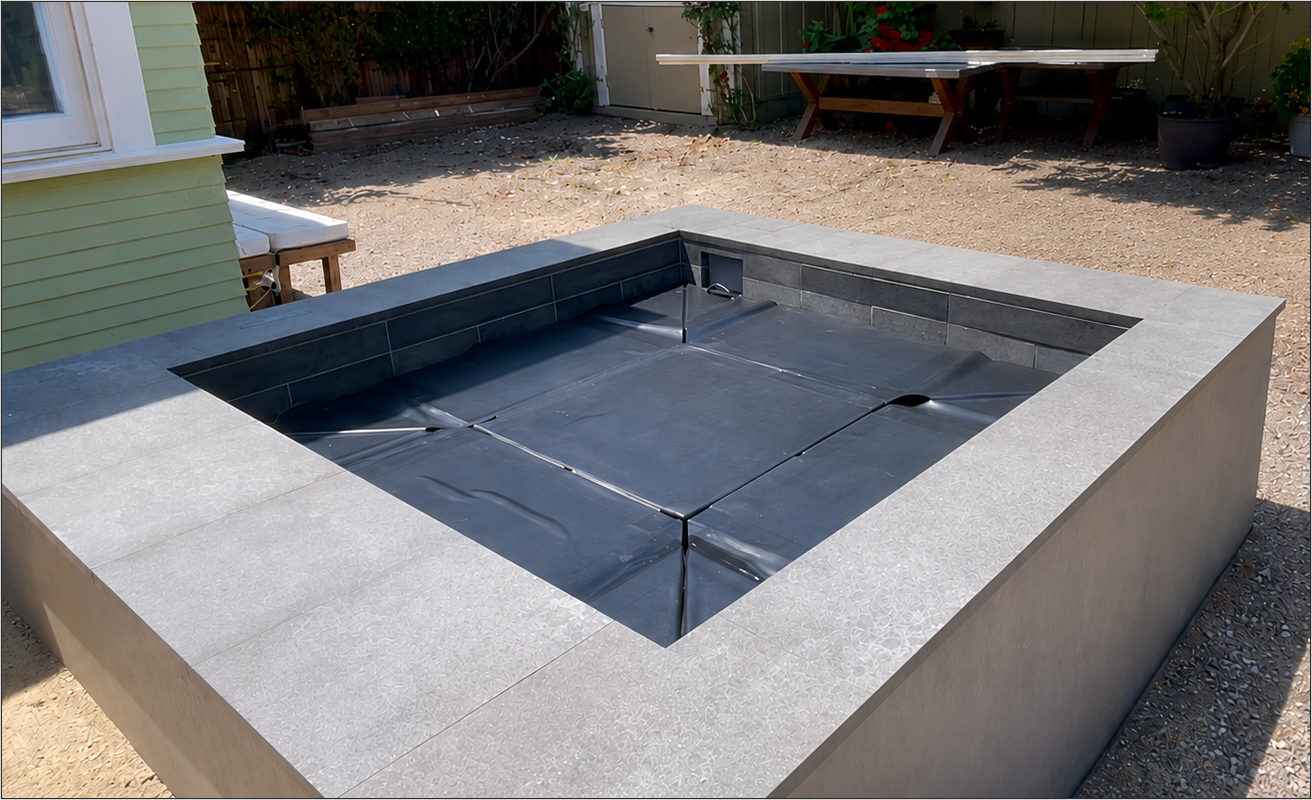
\includegraphics[
        width=5.55in,
        height=2.78in,
        keepaspectratio
    ]{deployed_functional_prototype}
};

\draw[DeepGreen,line width=0.8pt,rounded corners=7pt]
    ($(current page.north west)+(5.16in,-1.61in)$)
    rectangle
    ($(current page.north east)+(-0.42in,-4.47in)$);

\node[
    anchor=north west,
    text=Muted,
    font=\sffamily\fontsize{6.2}{6.9}\selectfont
]
at ($(current page.north west)+(5.18in,-4.54in)$)
{Functional foam model deployed over the sponsor's in-ground spa.};

% Image-strip title
\node[
    anchor=north west,
    text=DeepGreen,
    font=\sffamily\bfseries\fontsize{8.1}{8.8}\selectfont
]
at ($(current page.north west)+(0.43in,-4.78in)$)
{PRODUCT DEVELOPMENT AND FINAL ARCHITECTURE};

% Five-image development strip — CAD-first sequence
% Image 1: topside CAD
\node[anchor=center,inner sep=0pt]
at ($(current page.north west)+(1.47in,-5.73in)$)
{
    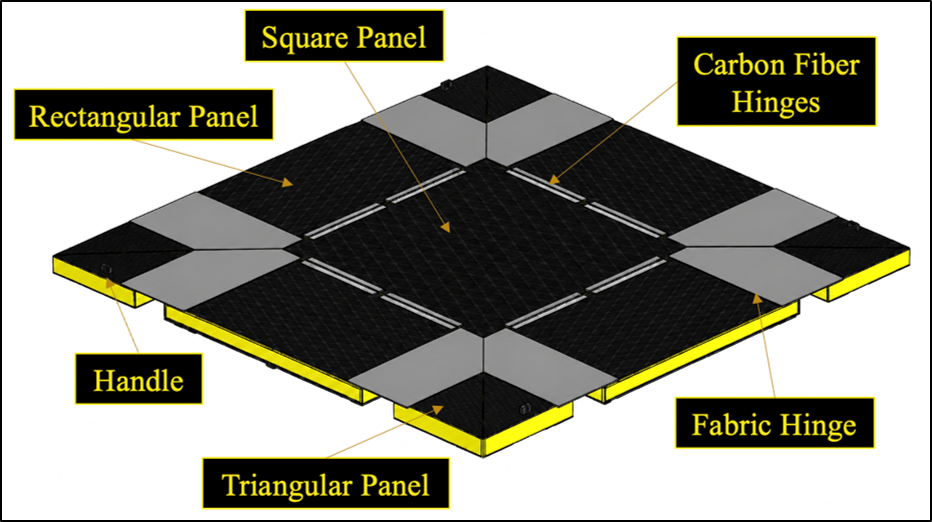
\includegraphics[
        width=1.92in,
        height=1.30in,
        keepaspectratio
    ]{Toro_Cover_topside_Cad}
};
\draw[RuleGray,line width=0.55pt,rounded corners=4pt]
    ($(current page.north west)+(0.43in,-5.04in)$)
    rectangle
    ($(current page.north west)+(2.51in,-6.43in)$);

% Image 2: underside CAD
\node[anchor=center,inner sep=0pt]
at ($(current page.north west)+(3.66in,-5.73in)$)
{
    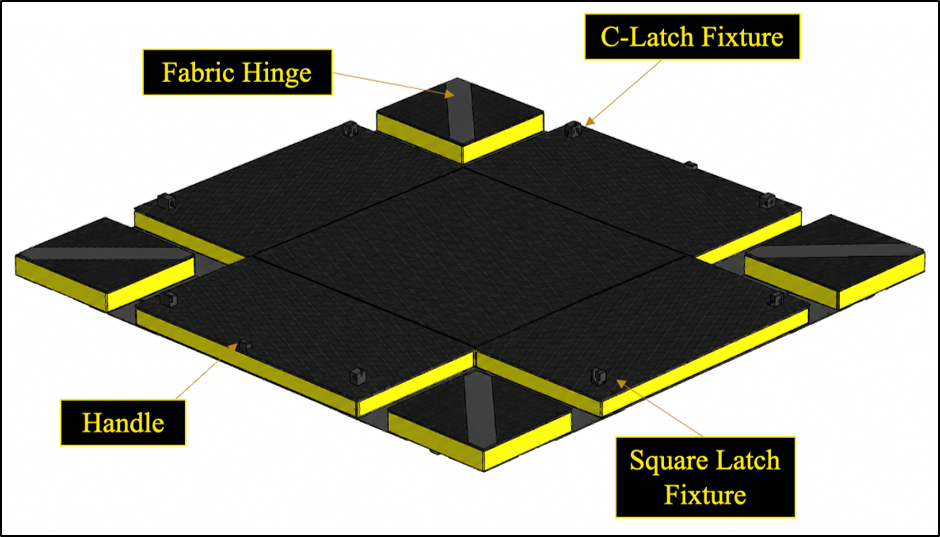
\includegraphics[
        width=1.92in,
        height=1.30in,
        keepaspectratio
    ]{toro_cover_underside_cad}
};
\draw[RuleGray,line width=0.55pt,rounded corners=4pt]
    ($(current page.north west)+(2.62in,-5.04in)$)
    rectangle
    ($(current page.north west)+(4.70in,-6.43in)$);

% Image 3: folded CAD
\node[anchor=center,inner sep=0pt]
at ($(current page.north west)+(5.85in,-5.73in)$)
{
    \includegraphics[
        width=1.92in,
        height=1.30in,
        keepaspectratio
    ]{\detokenize{Toro_Cover_folded Configuration}}
};
\draw[RuleGray,line width=0.55pt,rounded corners=4pt]
    ($(current page.north west)+(4.81in,-5.04in)$)
    rectangle
    ($(current page.north west)+(6.89in,-6.43in)$);

% Image 4: dual-use product concept
\node[anchor=center,inner sep=0pt]
at ($(current page.north west)+(8.04in,-5.73in)$)
{
    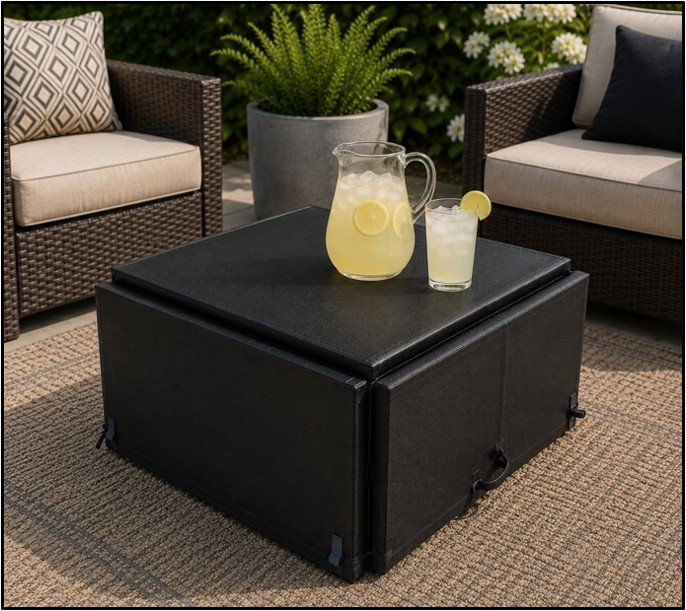
\includegraphics[
        width=1.92in,
        height=1.30in,
        keepaspectratio
    ]{generative_AI_concept_toro_cover_art}
};
\draw[RuleGray,line width=0.55pt,rounded corners=4pt]
    ($(current page.north west)+(7.00in,-5.04in)$)
    rectangle
    ($(current page.north west)+(9.08in,-6.43in)$);

% Image 5: folded foam functional prototype
% The portrait photograph is deliberately clipped to the landscape frame
% so the ottoman fills the card without extending beyond its border.
\begin{scope}
\clip[rounded corners=4pt]
    ($(current page.north west)+(9.19in,-5.04in)$)
    rectangle
    ($(current page.north east)+(-0.43in,-6.43in)$);

% Keep the original image proportions and center it within the existing card.
\node[anchor=center,inner sep=0pt]
at ($(current page.north west)+(9.88in,-5.735in)$)
{
    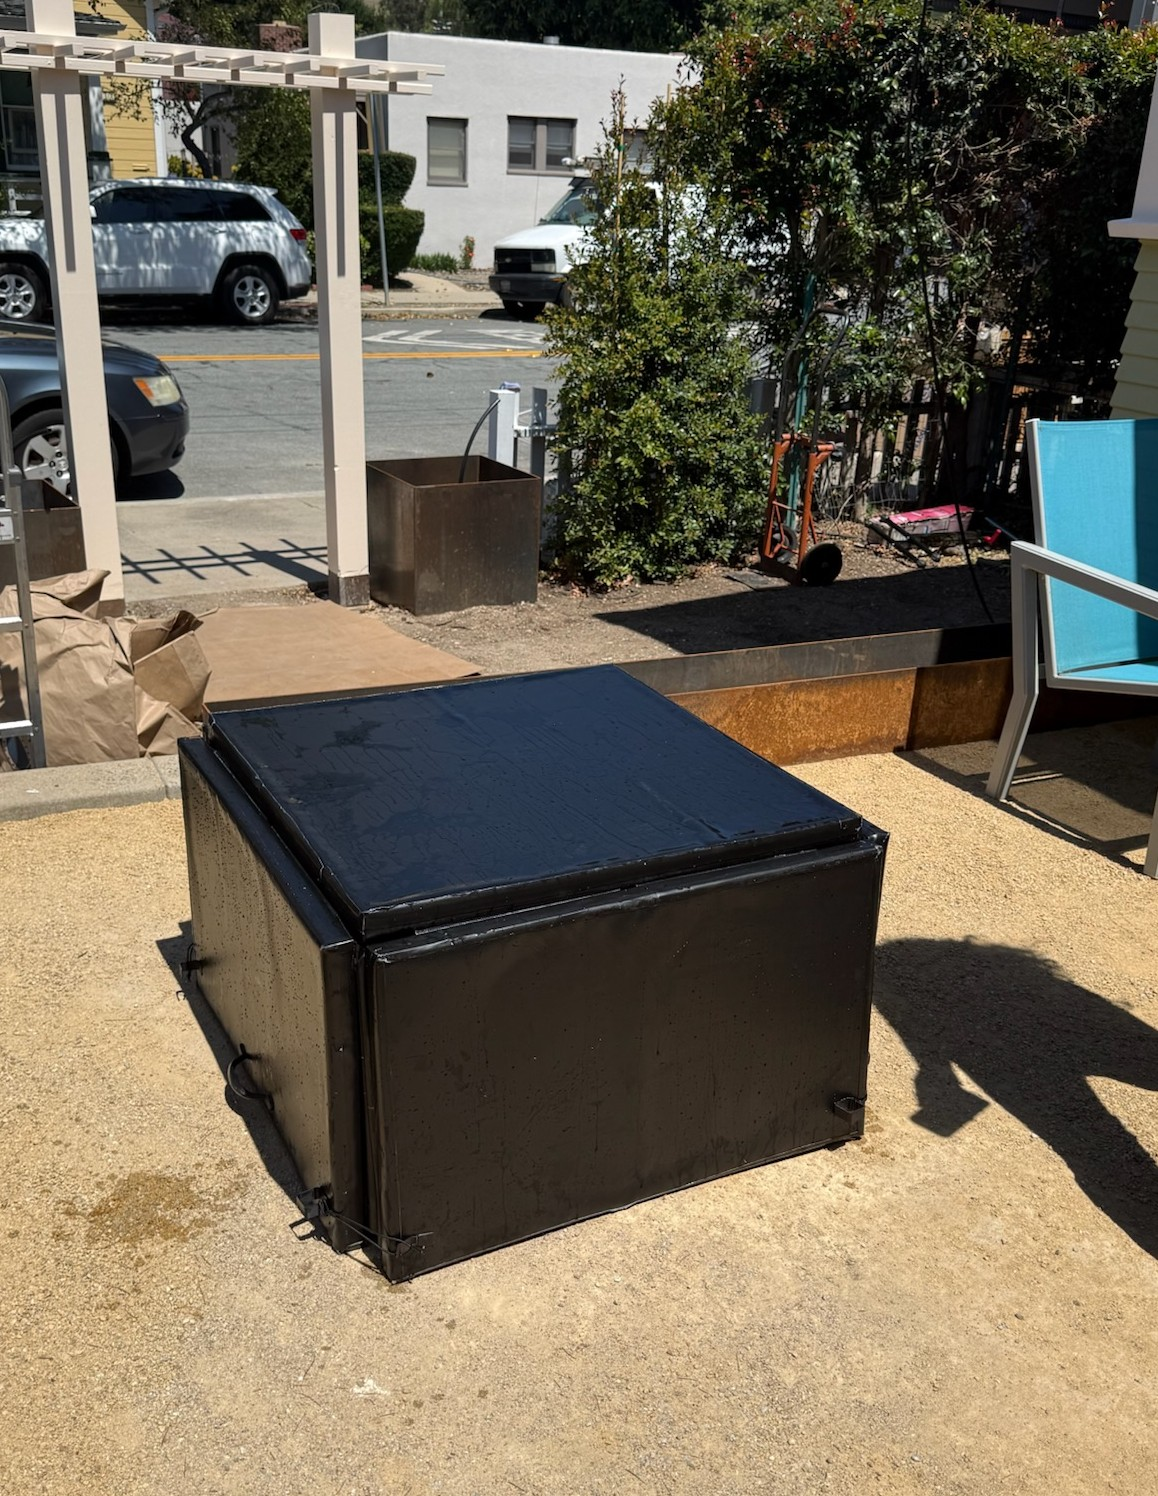
\includegraphics[
        width=1.58in,
        height=1.28in,
        keepaspectratio
    ]{foam_model_folded_backyard_image}
};
\end{scope}

\draw[RuleGray,line width=0.55pt,rounded corners=4pt]
    ($(current page.north west)+(9.19in,-5.04in)$)
    rectangle
    ($(current page.north east)+(-0.43in,-6.43in)$);

% Larger captions
\node[anchor=north,align=center,text width=1.95in,text=Muted,
      font=\sffamily\fontsize{6.8}{7.4}\selectfont]
at ($(current page.north west)+(1.47in,-6.49in)$)
{Topside panel architecture};

\node[anchor=north,align=center,text width=1.95in,text=Muted,
      font=\sffamily\fontsize{6.8}{7.4}\selectfont]
at ($(current page.north west)+(3.66in,-6.49in)$)
{Underside hinge architecture};

\node[anchor=north,align=center,text width=1.95in,text=Muted,
      font=\sffamily\fontsize{6.8}{7.4}\selectfont]
at ($(current page.north west)+(5.85in,-6.49in)$)
{Folded CAD configuration};

\node[anchor=north,align=center,text width=1.95in,text=Muted,
      font=\sffamily\fontsize{6.8}{7.4}\selectfont]
at ($(current page.north west)+(8.04in,-6.49in)$)
{Dual-use product vision};

\node[anchor=north,align=center,text width=1.95in,text=Muted,
      font=\sffamily\fontsize{6.8}{7.4}\selectfont]
at ($(current page.north west)+(9.88in,-6.49in)$)
{Folded foam prototype};

% Page 1 resource bar — centered and non-repeated resources
\fill[Panel,rounded corners=4pt]
    ($(current page.north west)+(0.43in,-7.05in)$)
    rectangle
    ($(current page.north east)+(-0.43in,-7.64in)$);
\draw[RuleGray,line width=0.5pt,rounded corners=4pt]
    ($(current page.north west)+(0.43in,-7.05in)$)
    rectangle
    ($(current page.north east)+(-0.43in,-7.64in)$);

\node[
    anchor=center,
    align=center,
    text=DeepGreen,
    font=\sffamily\bfseries\fontsize{6.9}{7.5}\selectfont
]
at ($(current page.north)+(0,-7.345in)$)
{\href{\ToroDrawingLink}{\faDraftingCompass\ DRAWING PACKAGE}
\hspace{24pt}
\href{\ToroDimensionsLink}{\faImage\ DIMENSION STUDY}
\hspace{24pt}
\href{\ToroProblemLink}{\faFileImage\ PROBLEM STATEMENT}};

% Footer
\node[
    anchor=south west,
    text=white,
    font=\sffamily\bfseries\fontsize{7.1}{7.7}\selectfont
]
at ($(current page.south west)+(0.42in,0.17in)$)
{\hyperlink{composites}{\faArrowLeft\ COMPOSITES}};

\node[
    anchor=south,
    text=white,
    font=\sffamily\fontsize{7.0}{7.6}\selectfont
]
at ($(current page.south)+(0,0.17in)$)
{TORO COVER \hspace{6pt} 1 / 3};

\node[
    anchor=south east,
    text=white,
    font=\sffamily\bfseries\fontsize{7.1}{7.7}\selectfont
]
at ($(current page.south east)+(-0.42in,0.17in)$)
{MANUFACTURING-DRIVEN DESIGN \faArrowRight};

\end{tikzpicture}


% ============================================================
% PAGE 2 — MANUFACTURING-DRIVEN DESIGN
% ============================================================

\clearpage
\thispagestyle{empty}
\hypertarget{toro-manufacturing}{}
\null

\begin{tikzpicture}[remember picture,overlay]

% Background and bars
\fill[white]
    (current page.south west)
    rectangle
    (current page.north east);

\fill[DeepGreen]
    (current page.north west)
    rectangle
    ($(current page.north east)+(0,-0.095in)$);

\fill[PolyGold]
    ($(current page.north west)+(0,-0.095in)$)
    rectangle
    ($(current page.north east)+(0,-0.14in)$);

\fill[DeepGreen]
    (current page.south west)
    rectangle
    ($(current page.south east)+(0,0.36in)$);

\fill[PolyGold]
    ($(current page.south west)+(0,0.36in)$)
    rectangle
    ($(current page.south east)+(0,0.405in)$);

% Header
\node[
    anchor=north west,
    text=PolyGold,
    font=\sffamily\bfseries\fontsize{8.1}{8.7}\selectfont
]
at ($(current page.north west)+(0.42in,-0.39in)$)
{TORO COVER \hspace{5pt}/\hspace{5pt} DESIGN FOR MANUFACTURABILITY};

\node[
    anchor=north west,
    text=DeepGreen,
    font=\bfseries\fontsize{23}{24}\selectfont
]
at ($(current page.north west)+(0.40in,-0.67in)$)
{THE ENVELOPE METHOD};

\node[
    anchor=north west,
    text=Muted,
    font=\sffamily\fontsize{8.7}{9.6}\selectfont
]
at ($(current page.north west)+(0.42in,-1.12in)$)
{A one-layup process developed for unusually thick insulated composite sandwich panels};

\fill[PolyGold]
    ($(current page.north west)+(0.42in,-1.36in)$)
    rectangle
    ($(current page.north west)+(5.30in,-1.315in)$);

% Process explanation
\fill[SoftGold,rounded corners=5pt]
    ($(current page.north west)+(0.42in,-1.61in)$)
    rectangle
    ($(current page.north east)+(-0.42in,-2.90in)$);

\fill[PolyGold]
    ($(current page.north west)+(0.42in,-1.61in)$)
    rectangle
    ($(current page.north west)+(0.52in,-2.90in)$);

\node[
    anchor=north west,
    text=DeepGreen,
    font=\sffamily\bfseries\fontsize{7.9}{8.6}\selectfont
]
at ($(current page.north west)+(0.67in,-1.76in)$)
{PROCESS INNOVATION};

\node[
    anchor=north west,
    align=left,
    text width=9.55in,
    text=Ink,
    font=\fontsize{7.35}{8.75}\selectfont
]
at ($(current page.north west)+(0.67in,-2.02in)$)
{
Weight reduction and insulation were both essential, leading to the selection of an
XPS foam core. Because XPS could not tolerate composite heat-cure temperatures, prepreg
processing was not practical and the panels had to be manufactured by wet layup with a
room-temperature cure. To simplify this process, I waterjet-cut XPS perimeter strips from
excess foam and placed them around each core inside the vacuum enclosure. Under vacuum,
the top and bottom carbon skins met along the panel sides and compressed against this
border, eliminating a separate edge-banding layup and reducing corner pleating.
};

% Workflow title
\node[
    anchor=north west,
    text=DeepGreen,
    font=\sffamily\bfseries\fontsize{8.0}{8.7}\selectfont
]
at ($(current page.north west)+(0.43in,-3.06in)$)
{MANUFACTURING WORKFLOW};

% Row 1 image 1
\node[anchor=center,inner sep=0pt]
at ($(current page.north west)+(2.07in,-4.105in)$)
{
    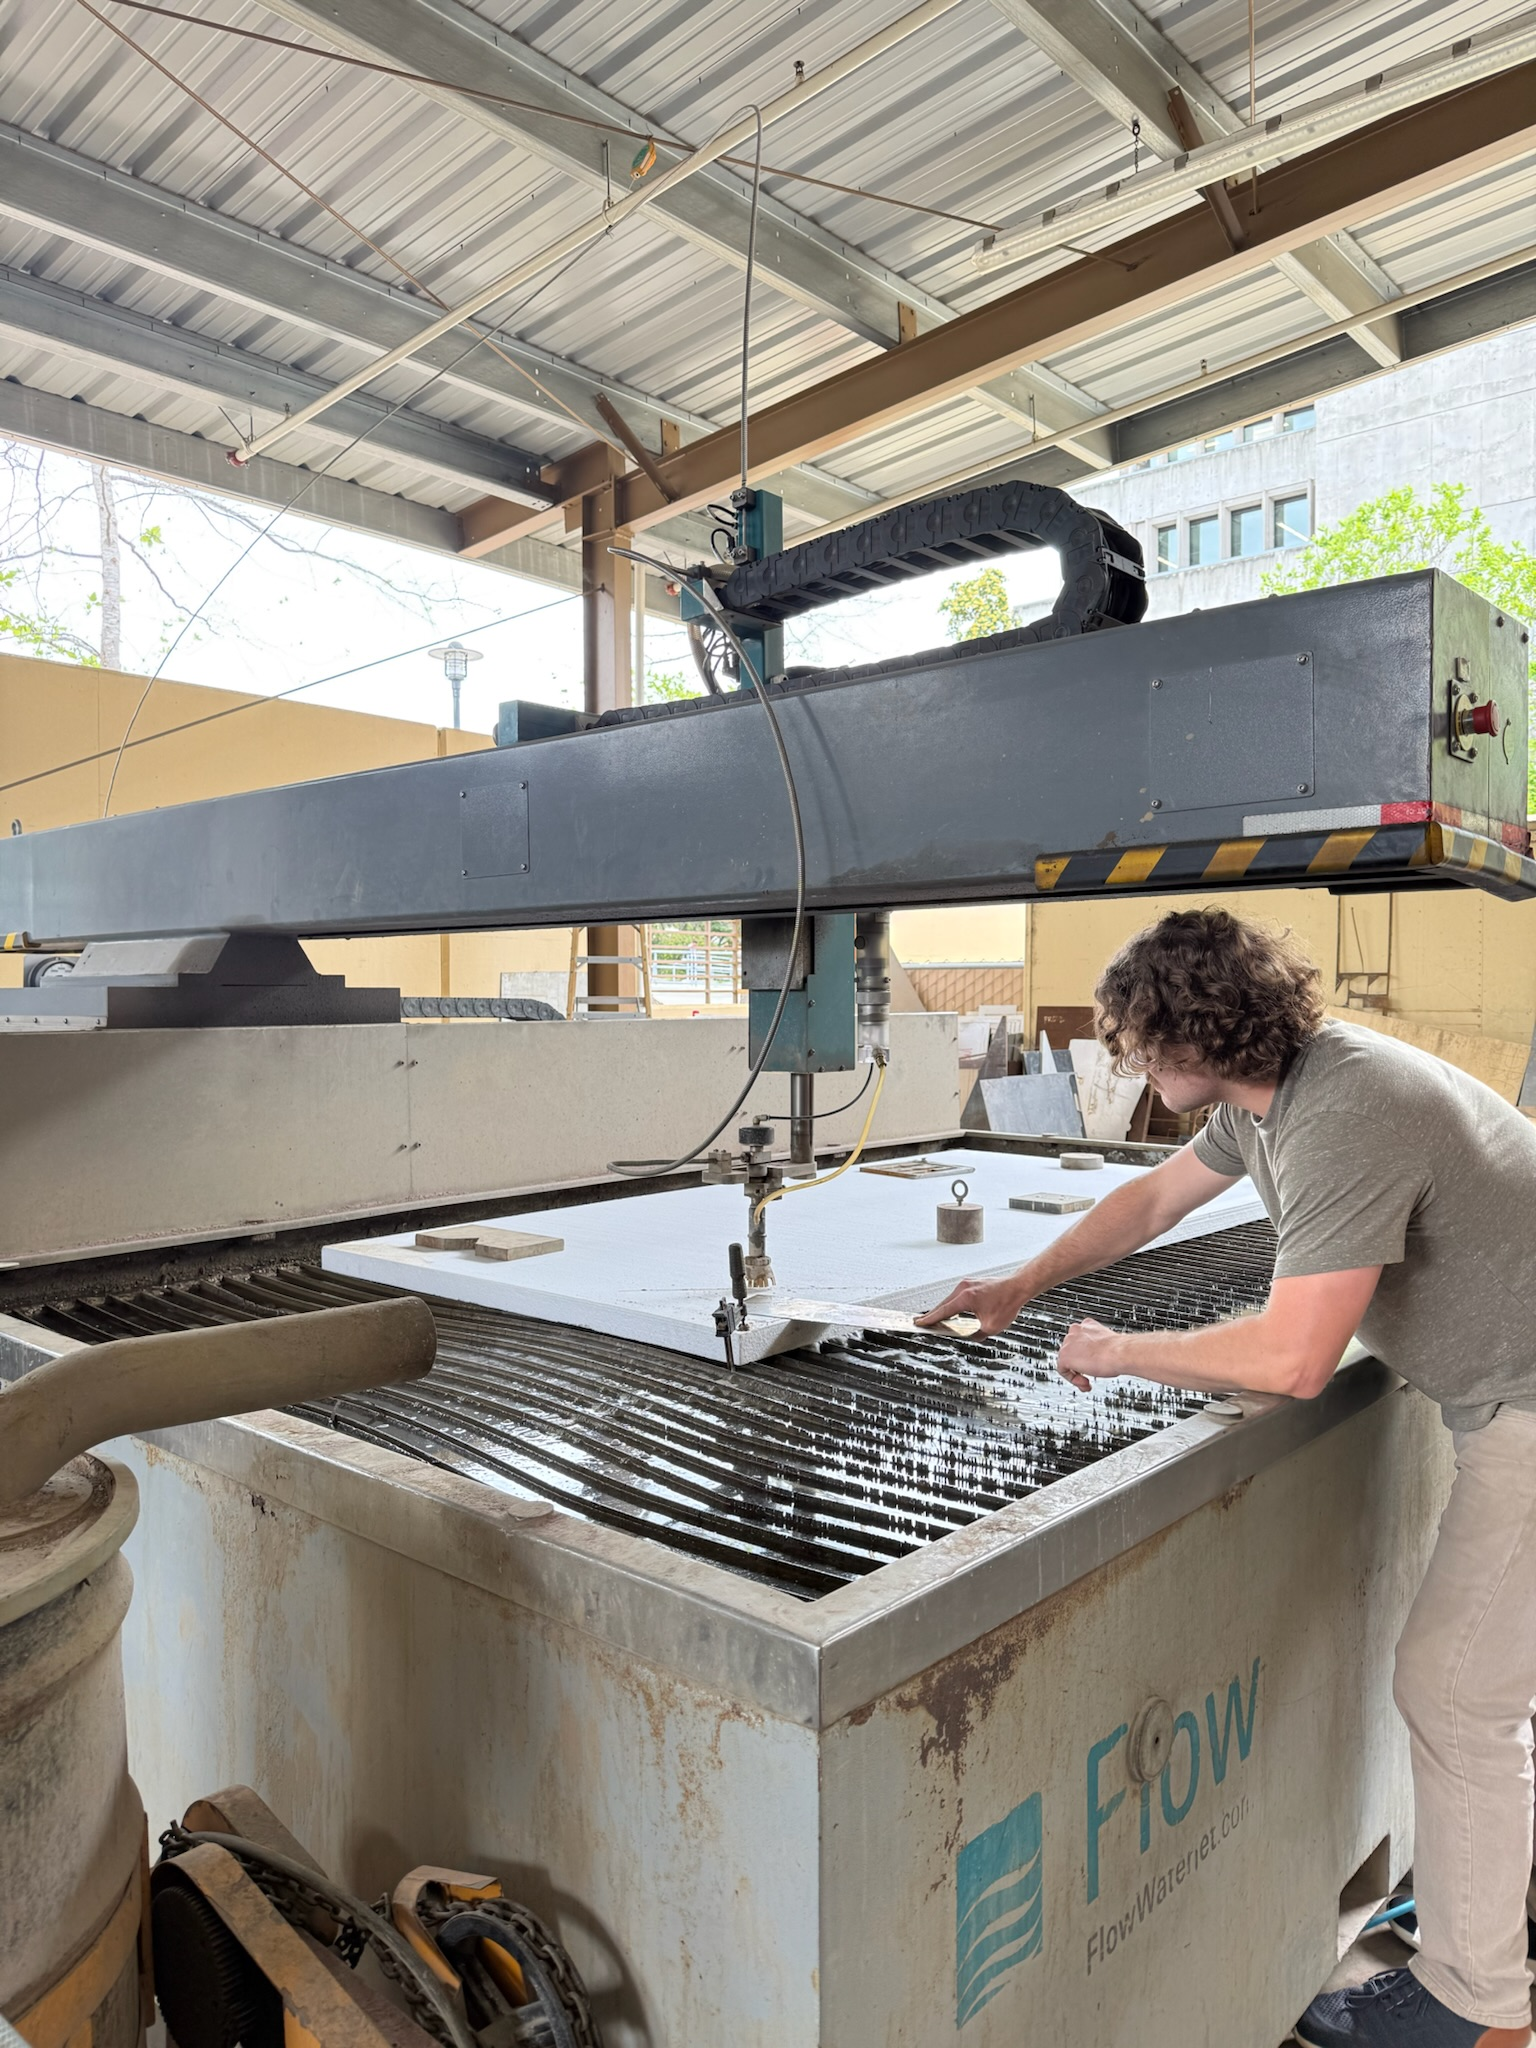
\includegraphics[
        width=3.10in,
        height=1.40in,
        keepaspectratio
    ]{waterjet_foam}
};
\draw[RuleGray,line width=0.55pt,rounded corners=4pt]
    ($(current page.north west)+(0.43in,-3.36in)$)
    rectangle
    ($(current page.north west)+(3.71in,-4.85in)$);

% Row 1 image 2
\node[anchor=center,inner sep=0pt]
at ($(current page.north west)+(5.50in,-4.105in)$)
{
    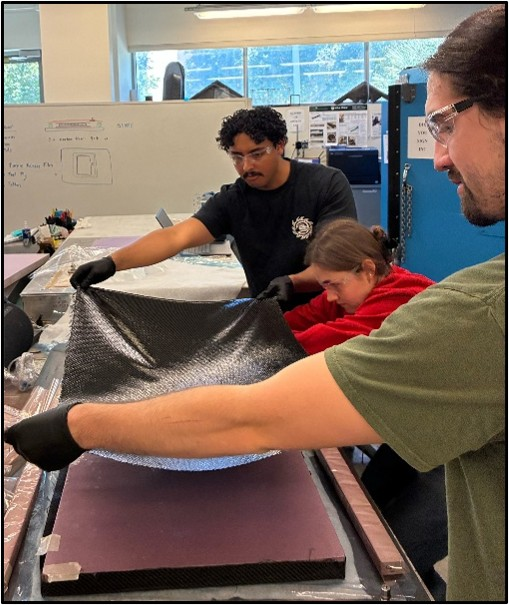
\includegraphics[
        width=3.10in,
        height=1.40in,
        keepaspectratio
    ]{group_layup}
};
\draw[RuleGray,line width=0.55pt,rounded corners=4pt]
    ($(current page.north west)+(3.86in,-3.36in)$)
    rectangle
    ($(current page.north west)+(7.14in,-4.85in)$);

% Row 1 image 3
\node[anchor=center,inner sep=0pt]
at ($(current page.north west)+(8.935in,-4.105in)$)
{
    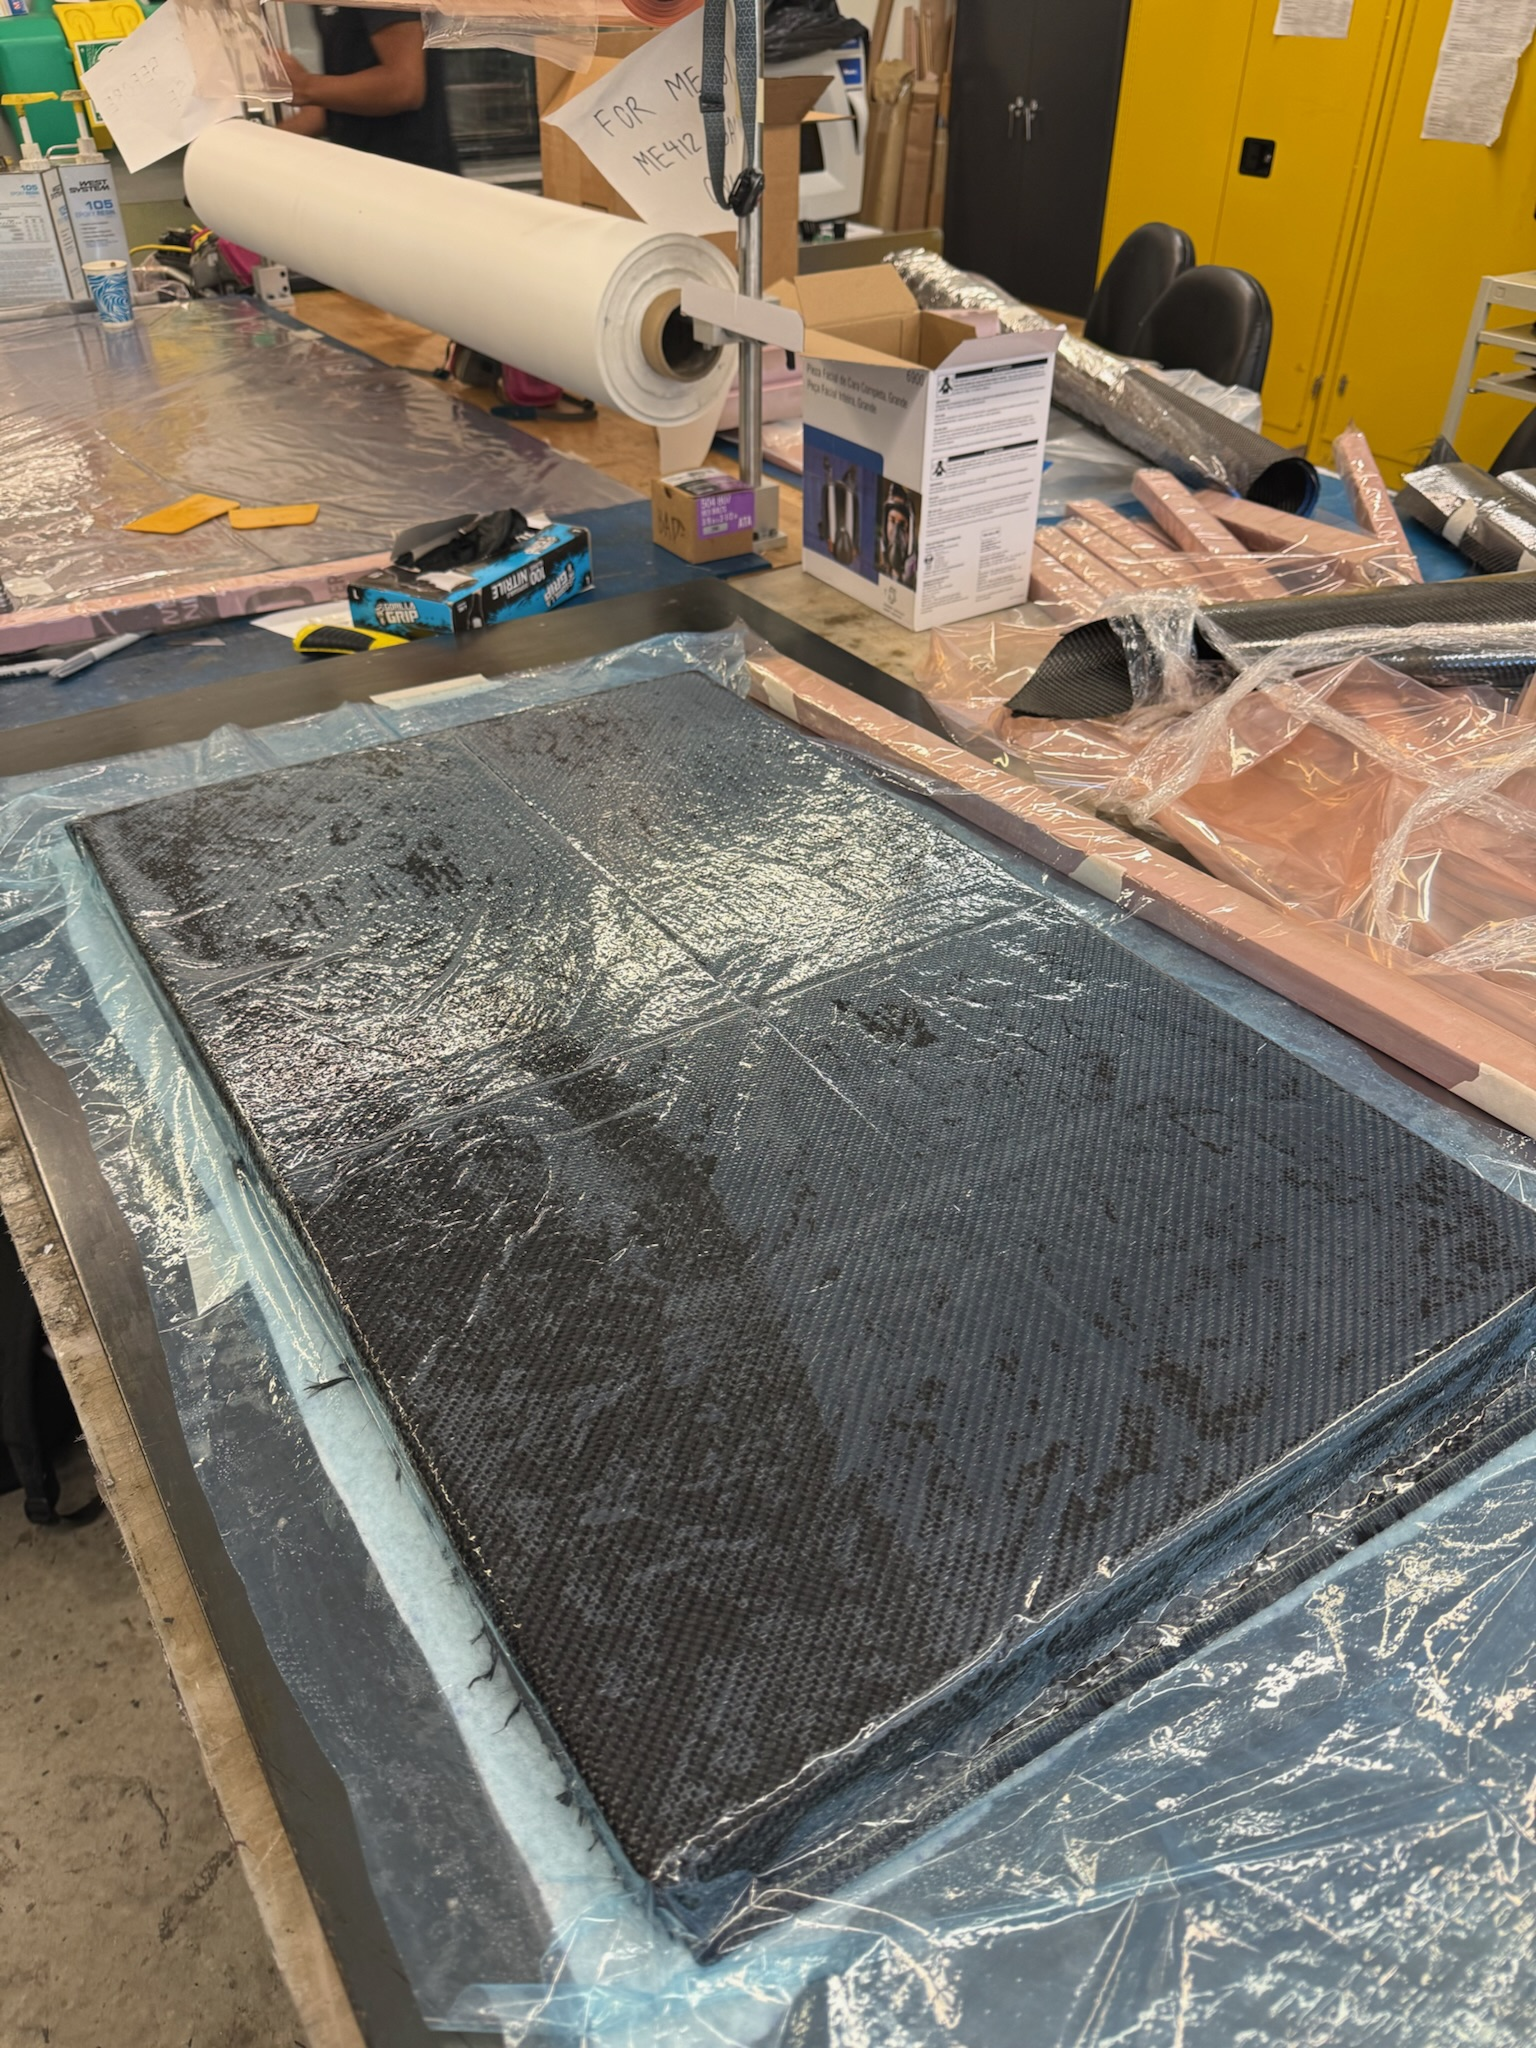
\includegraphics[
        width=3.10in,
        height=1.40in,
        keepaspectratio
    ]{blue_perforrated_film_layup}
};
\draw[RuleGray,line width=0.55pt,rounded corners=4pt]
    ($(current page.north west)+(7.29in,-3.36in)$)
    rectangle
    ($(current page.north east)+(-0.42in,-4.85in)$);

% Row 1 captions
\node[anchor=north,text=Muted,font=\sffamily\fontsize{6.7}{7.3}\selectfont]
at ($(current page.north west)+(2.07in,-4.90in)$)
{1. Waterjet-cut core and perimeter geometry};

\node[anchor=north,text=Muted,font=\sffamily\fontsize{6.7}{7.3}\selectfont]
at ($(current page.north west)+(5.50in,-4.90in)$)
{2. Team wet layup under my process guidance};

\node[anchor=north,text=Muted,font=\sffamily\fontsize{6.7}{7.3}\selectfont]
at ($(current page.north west)+(8.935in,-4.90in)$)
{3. Perforated film, breather, and vacuum enclosure};

% Row 2 image 1
\node[anchor=center,inner sep=0pt]
at ($(current page.north west)+(2.07in,-5.875in)$)
{
    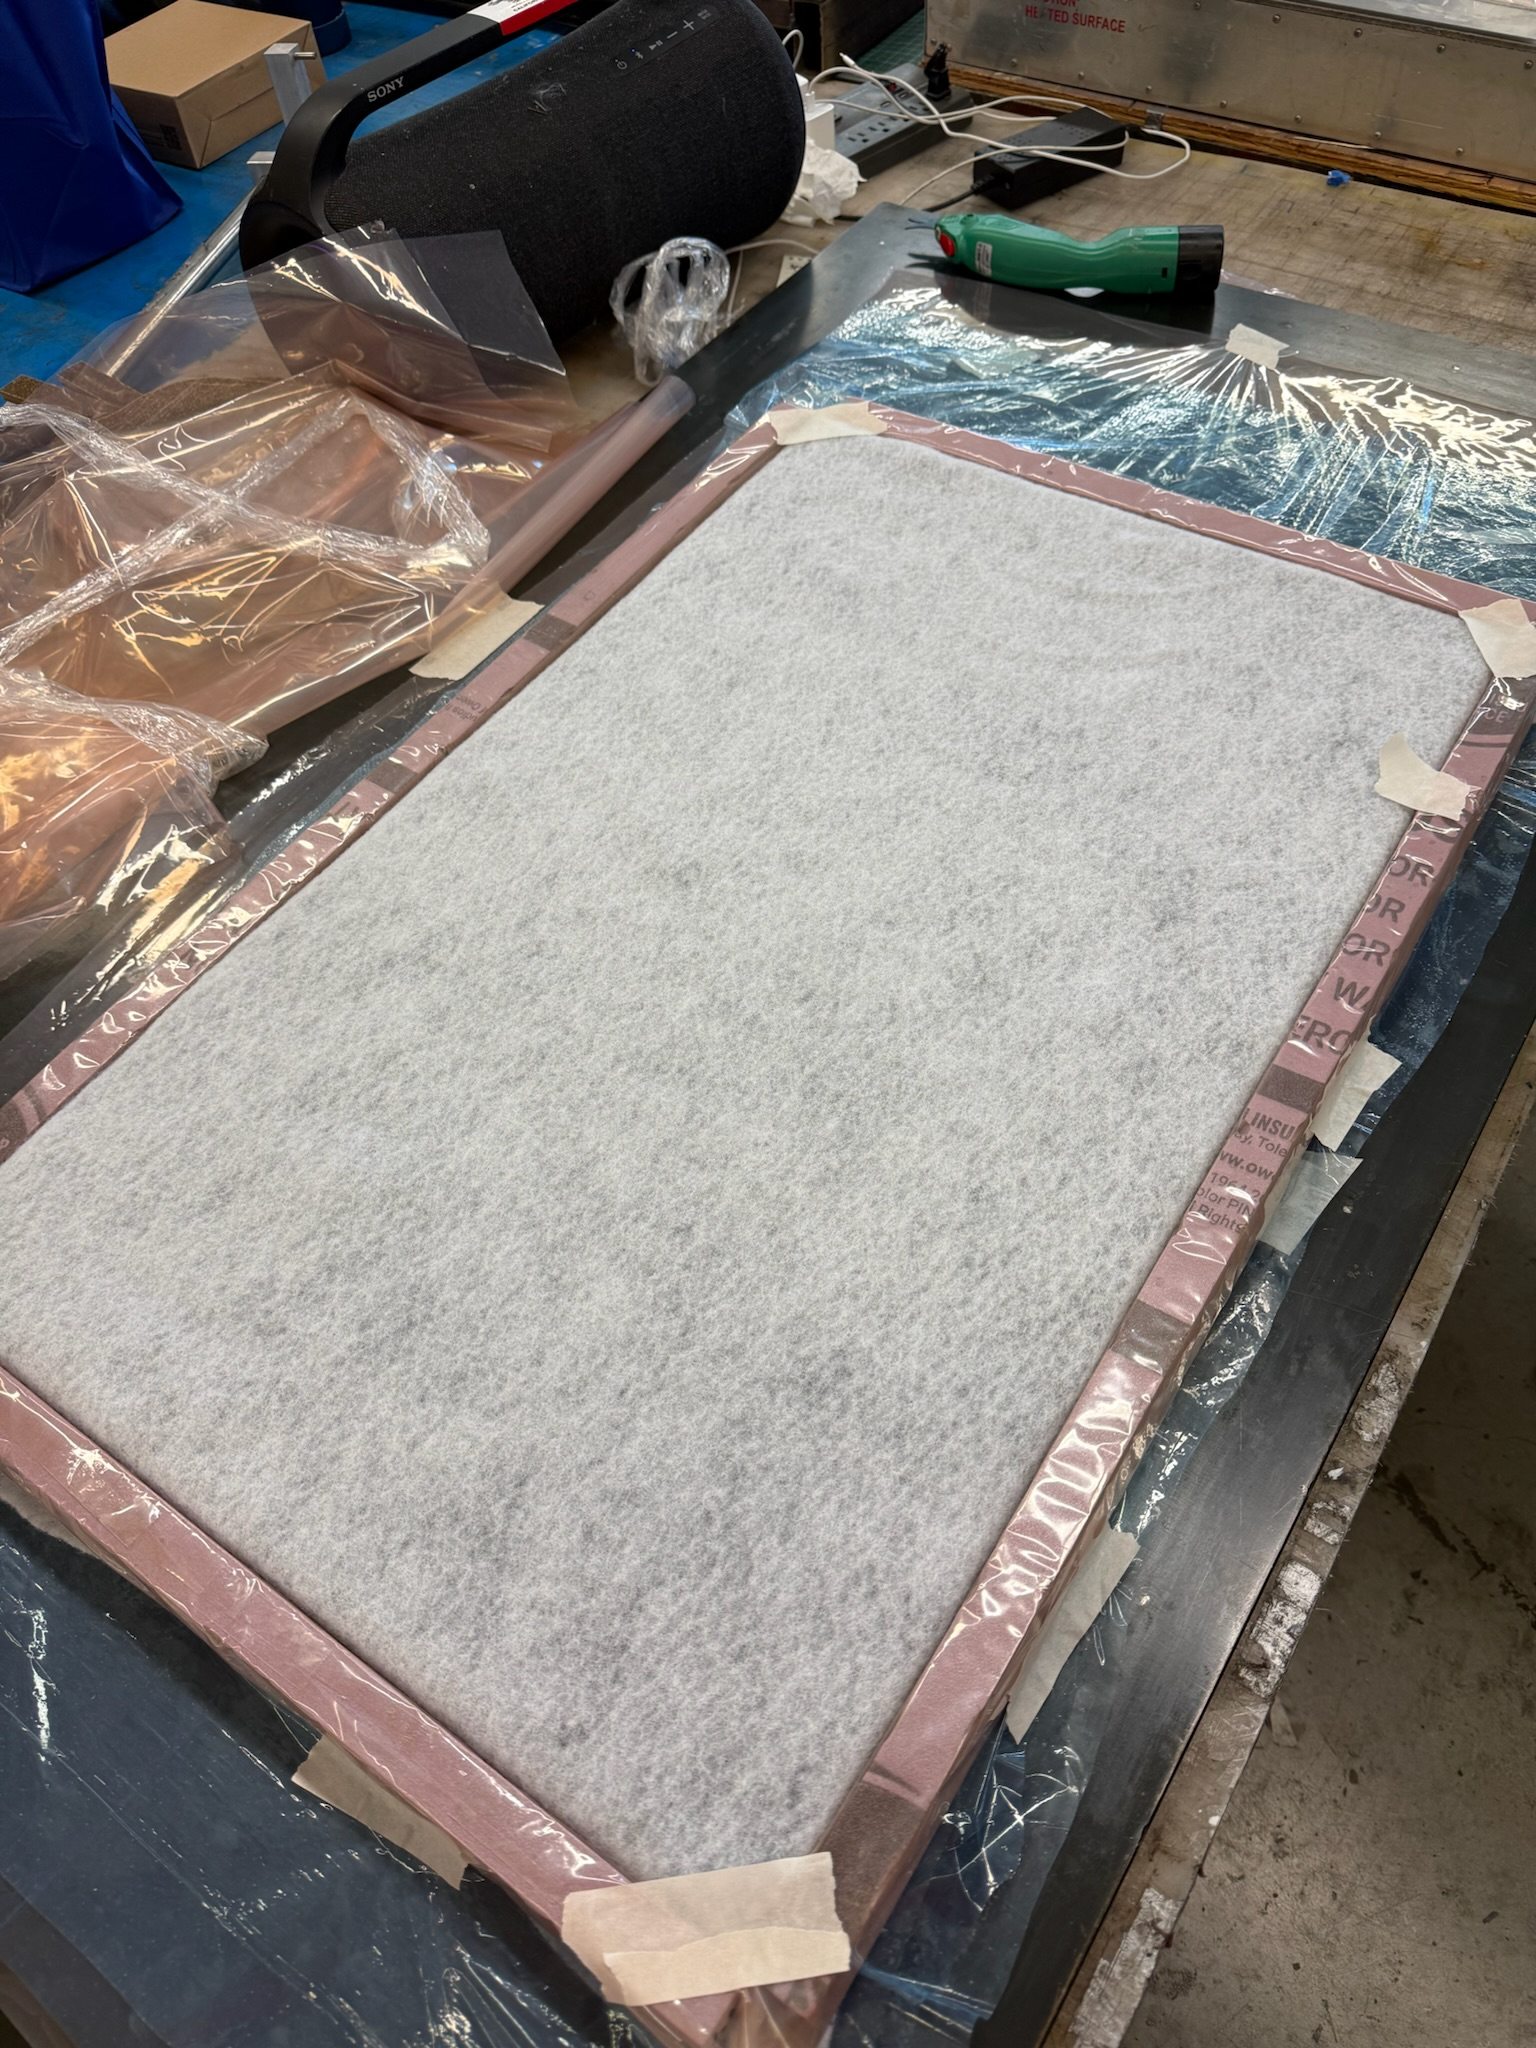
\includegraphics[
        width=3.10in,
        height=1.40in,
        keepaspectratio
    ]{completed_layup}
};
\draw[RuleGray,line width=0.55pt,rounded corners=4pt]
    ($(current page.north west)+(0.43in,-5.13in)$)
    rectangle
    ($(current page.north west)+(3.71in,-6.62in)$);

% Row 2 image 2 — oven chamber used only as a reliable vacuum enclosure; no heat applied
\node[anchor=center,inner sep=0pt]
at ($(current page.north west)+(5.50in,-5.875in)$)
{
    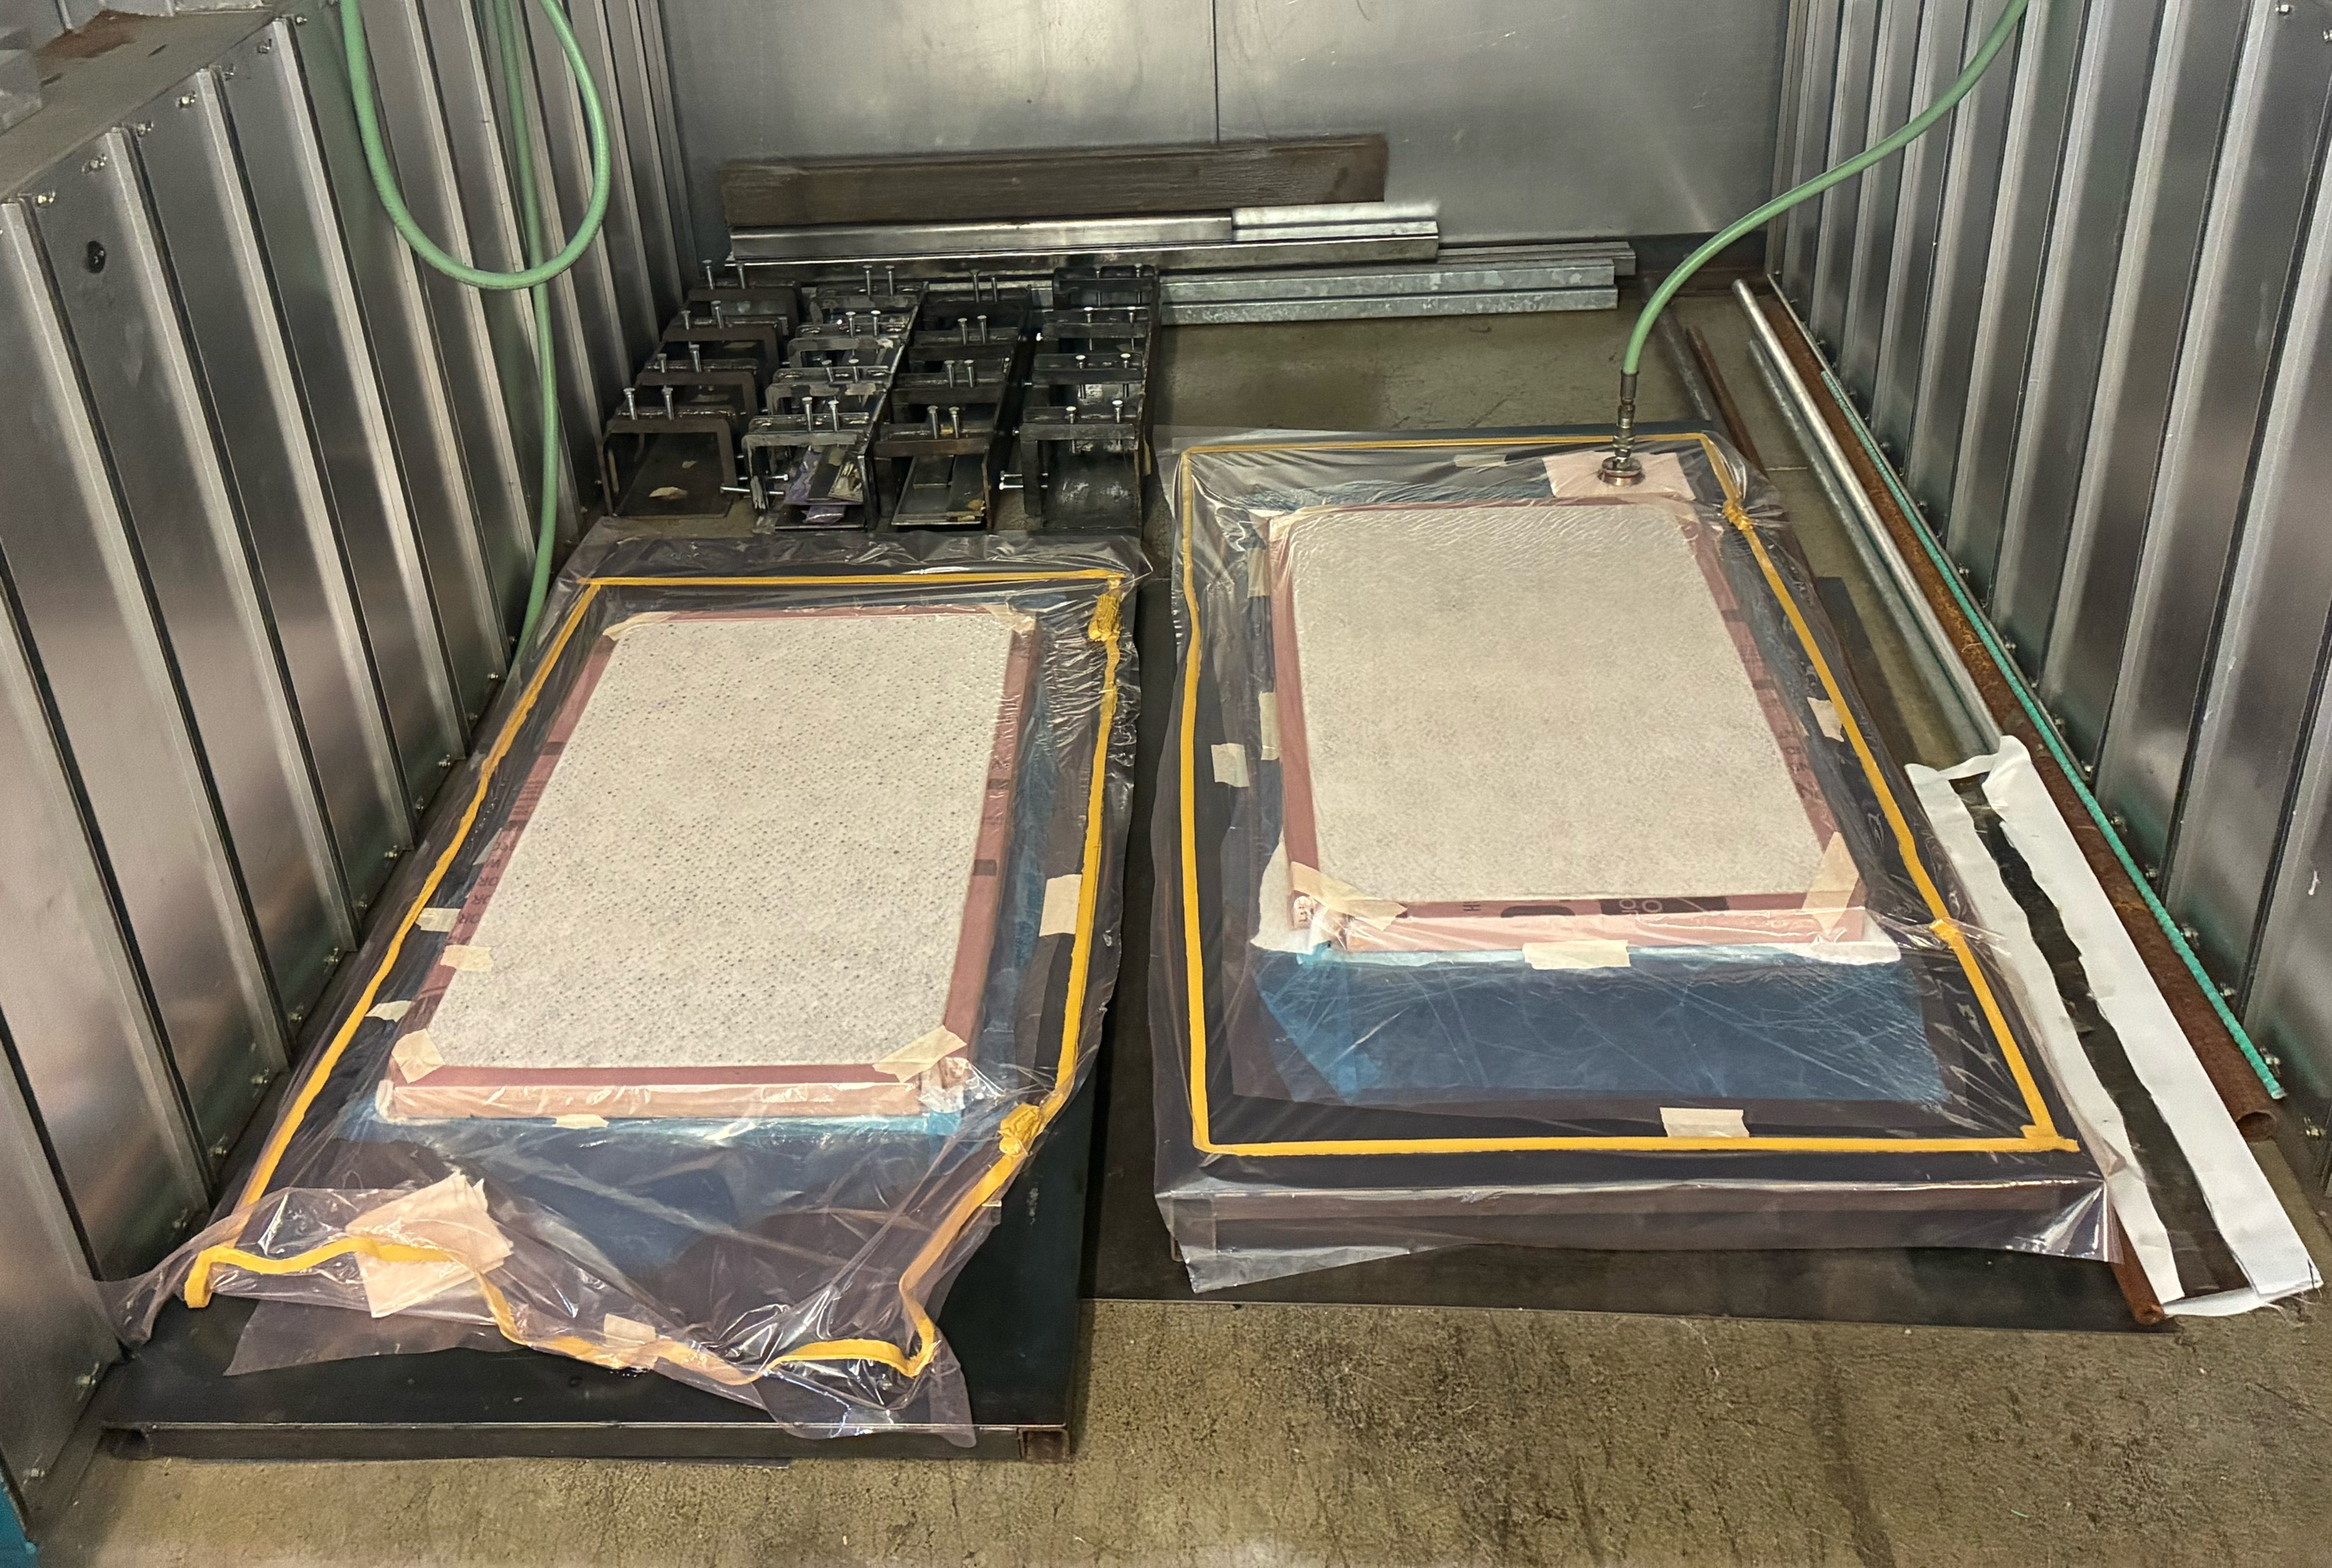
\includegraphics[
        width=3.10in,
        height=1.40in,
        keepaspectratio
    ]{layups_in_composite_oven_under_vacuumPressure}
};
\draw[RuleGray,line width=0.55pt,rounded corners=4pt]
    ($(current page.north west)+(3.86in,-5.13in)$)
    rectangle
    ($(current page.north west)+(7.14in,-6.62in)$);

% Row 2 image 3
\node[anchor=center,inner sep=0pt]
at ($(current page.north west)+(8.935in,-5.875in)$)
{
    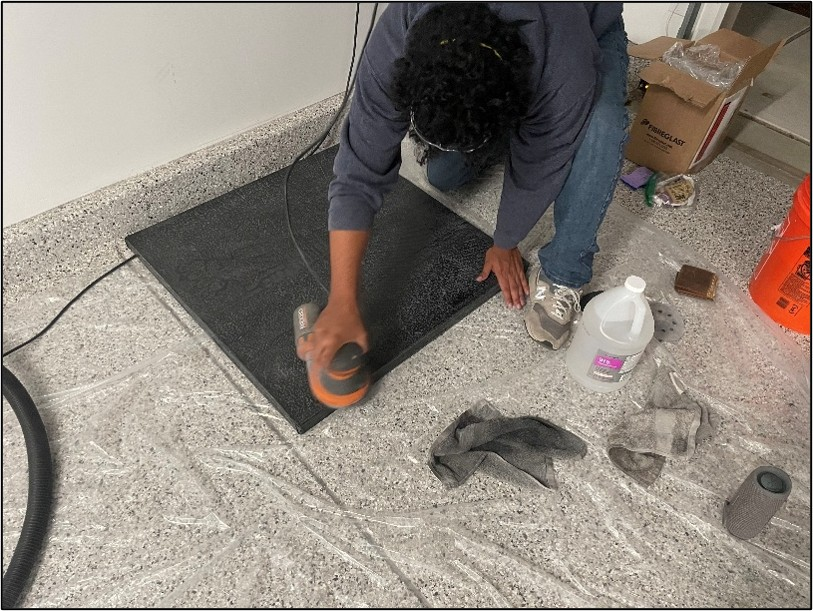
\includegraphics[
        width=3.10in,
        height=1.40in,
        keepaspectratio
    ]{garage_sanding}
};
\draw[RuleGray,line width=0.55pt,rounded corners=4pt]
    ($(current page.north west)+(7.29in,-5.13in)$)
    rectangle
    ($(current page.north east)+(-0.42in,-6.62in)$);

% Row 2 captions
\node[anchor=north,text=Muted,font=\sffamily\fontsize{6.7}{7.3}\selectfont]
at ($(current page.north west)+(2.07in,-6.67in)$)
{4. Fully saturated carbon skin and foam sandwich};

\node[anchor=north,text=Muted,font=\sffamily\fontsize{6.7}{7.3}\selectfont]
at ($(current page.north west)+(5.50in,-6.67in)$)
{5. Room-temperature cure under continuous vacuum};

\node[anchor=north,text=Muted,font=\sffamily\fontsize{6.7}{7.3}\selectfont]
at ($(current page.north west)+(8.935in,-6.67in)$)
{6. Post-processing and surface preparation};

% Bottom callouts
\fill[Panel,rounded corners=4pt]
    ($(current page.north west)+(0.43in,-6.95in)$)
    rectangle
    ($(current page.north west)+(5.48in,-7.60in)$);

\draw[RuleGray,line width=0.55pt,rounded corners=4pt]
    ($(current page.north west)+(0.43in,-6.95in)$)
    rectangle
    ($(current page.north west)+(5.48in,-7.60in)$);

\node[
    anchor=north west,
    text=DeepGreen,
    font=\sffamily\bfseries\fontsize{7.0}{7.6}\selectfont
]
at ($(current page.north west)+(0.63in,-7.08in)$)
{FROM THREE LAYUPS TO ONE};

\node[
    anchor=north west,
    align=left,
    text width=4.56in,
    text=Ink,
    font=\fontsize{6.45}{7.45}\selectfont
]
at ($(current page.north west)+(0.63in,-7.29in)$)
{
The Envelope Method reduced labor, cure cycles, handling,
alignment risk, and time spent forming numerous vacuum-bag
pleats around the 1.5-inch-thick XPS panels.
};

\fill[Panel,rounded corners=4pt]
    ($(current page.north west)+(5.68in,-6.95in)$)
    rectangle
    ($(current page.north east)+(-0.42in,-7.60in)$);

\draw[RuleGray,line width=0.55pt,rounded corners=4pt]
    ($(current page.north west)+(5.68in,-6.95in)$)
    rectangle
    ($(current page.north east)+(-0.42in,-7.60in)$);

\node[
    anchor=north west,
    text=DeepGreen,
    font=\sffamily\bfseries\fontsize{7.0}{7.6}\selectfont
]
at ($(current page.north west)+(5.88in,-7.08in)$)
{WHY SURFACE-BONDED HARDWARE};

\node[
    anchor=north west,
    align=left,
    text width=4.55in,
    text=Ink,
    font=\fontsize{6.45}{7.45}\selectfont
]
at ($(current page.north west)+(5.88in,-7.29in)$)
{
Adhesively bonded hinges and fixtures preserved the clean
composite exterior and avoided drilled inserts, foam-core
crushing, added stress concentrations, and new leak paths.
};


% Footer
\node[
    anchor=south west,
    text=white,
    font=\sffamily\bfseries\fontsize{7.1}{7.7}\selectfont
]
at ($(current page.south west)+(0.42in,0.17in)$)
{\faArrowLeft\ PRODUCT ARCHITECTURE};

\node[
    anchor=south,
    text=white,
    font=\sffamily\fontsize{7.0}{7.6}\selectfont
]
at ($(current page.south)+(0,0.17in)$)
{TORO COVER \hspace{6pt} 2 / 3};

\node[
    anchor=south east,
    text=white,
    font=\sffamily\bfseries\fontsize{7.1}{7.7}\selectfont
]
at ($(current page.south east)+(-0.42in,0.17in)$)
{VALIDATION \& TAKEAWAYS \faArrowRight};

\end{tikzpicture}


% ============================================================
% PAGE 3 — FINISHING, VALIDATION, AND TAKEAWAYS
% ============================================================

\clearpage
\thispagestyle{empty}
\hypertarget{toro-results}{}
\null

\begin{tikzpicture}[remember picture,overlay]

% Background and bars
\fill[white]
    (current page.south west)
    rectangle
    (current page.north east);

\fill[DeepGreen]
    (current page.north west)
    rectangle
    ($(current page.north east)+(0,-0.095in)$);

\fill[PolyGold]
    ($(current page.north west)+(0,-0.095in)$)
    rectangle
    ($(current page.north east)+(0,-0.14in)$);

\fill[DeepGreen]
    (current page.south west)
    rectangle
    ($(current page.south east)+(0,0.36in)$);

\fill[PolyGold]
    ($(current page.south west)+(0,0.36in)$)
    rectangle
    ($(current page.south east)+(0,0.405in)$);

% Header
\node[
    anchor=north west,
    text=PolyGold,
    font=\sffamily\bfseries\fontsize{8.1}{8.7}\selectfont
]
at ($(current page.north west)+(0.42in,-0.39in)$)
{TORO COVER \hspace{5pt}/\hspace{5pt} VALIDATION AND ENGINEERING TAKEAWAYS};

\node[
    anchor=north west,
    text=DeepGreen,
    font=\bfseries\fontsize{22.5}{23.5}\selectfont
]
at ($(current page.north west)+(0.40in,-0.67in)$)
{FROM PROTOTYPE TO PRODUCT PATHWAY};

\node[
    anchor=north west,
    text=Muted,
    font=\sffamily\fontsize{8.7}{9.6}\selectfont
]
at ($(current page.north west)+(0.42in,-1.12in)$)
{Environmental protection, usability testing, scope decisions, and lessons from technical leadership};

\fill[PolyGold]
    ($(current page.north west)+(0.42in,-1.36in)$)
    rectangle
    ($(current page.north west)+(5.8in,-1.315in)$);

% Finishing title
\node[
    anchor=north west,
    text=DeepGreen,
    font=\sffamily\bfseries\fontsize{8.0}{8.7}\selectfont
]
at ($(current page.north west)+(0.43in,-1.62in)$)
{OUTDOOR FINISHING AND ENVIRONMENTAL PROTECTION};

% Image 1
\node[anchor=center,inner sep=0pt]
at ($(current page.north west)+(1.705in,-2.655in)$)
{
    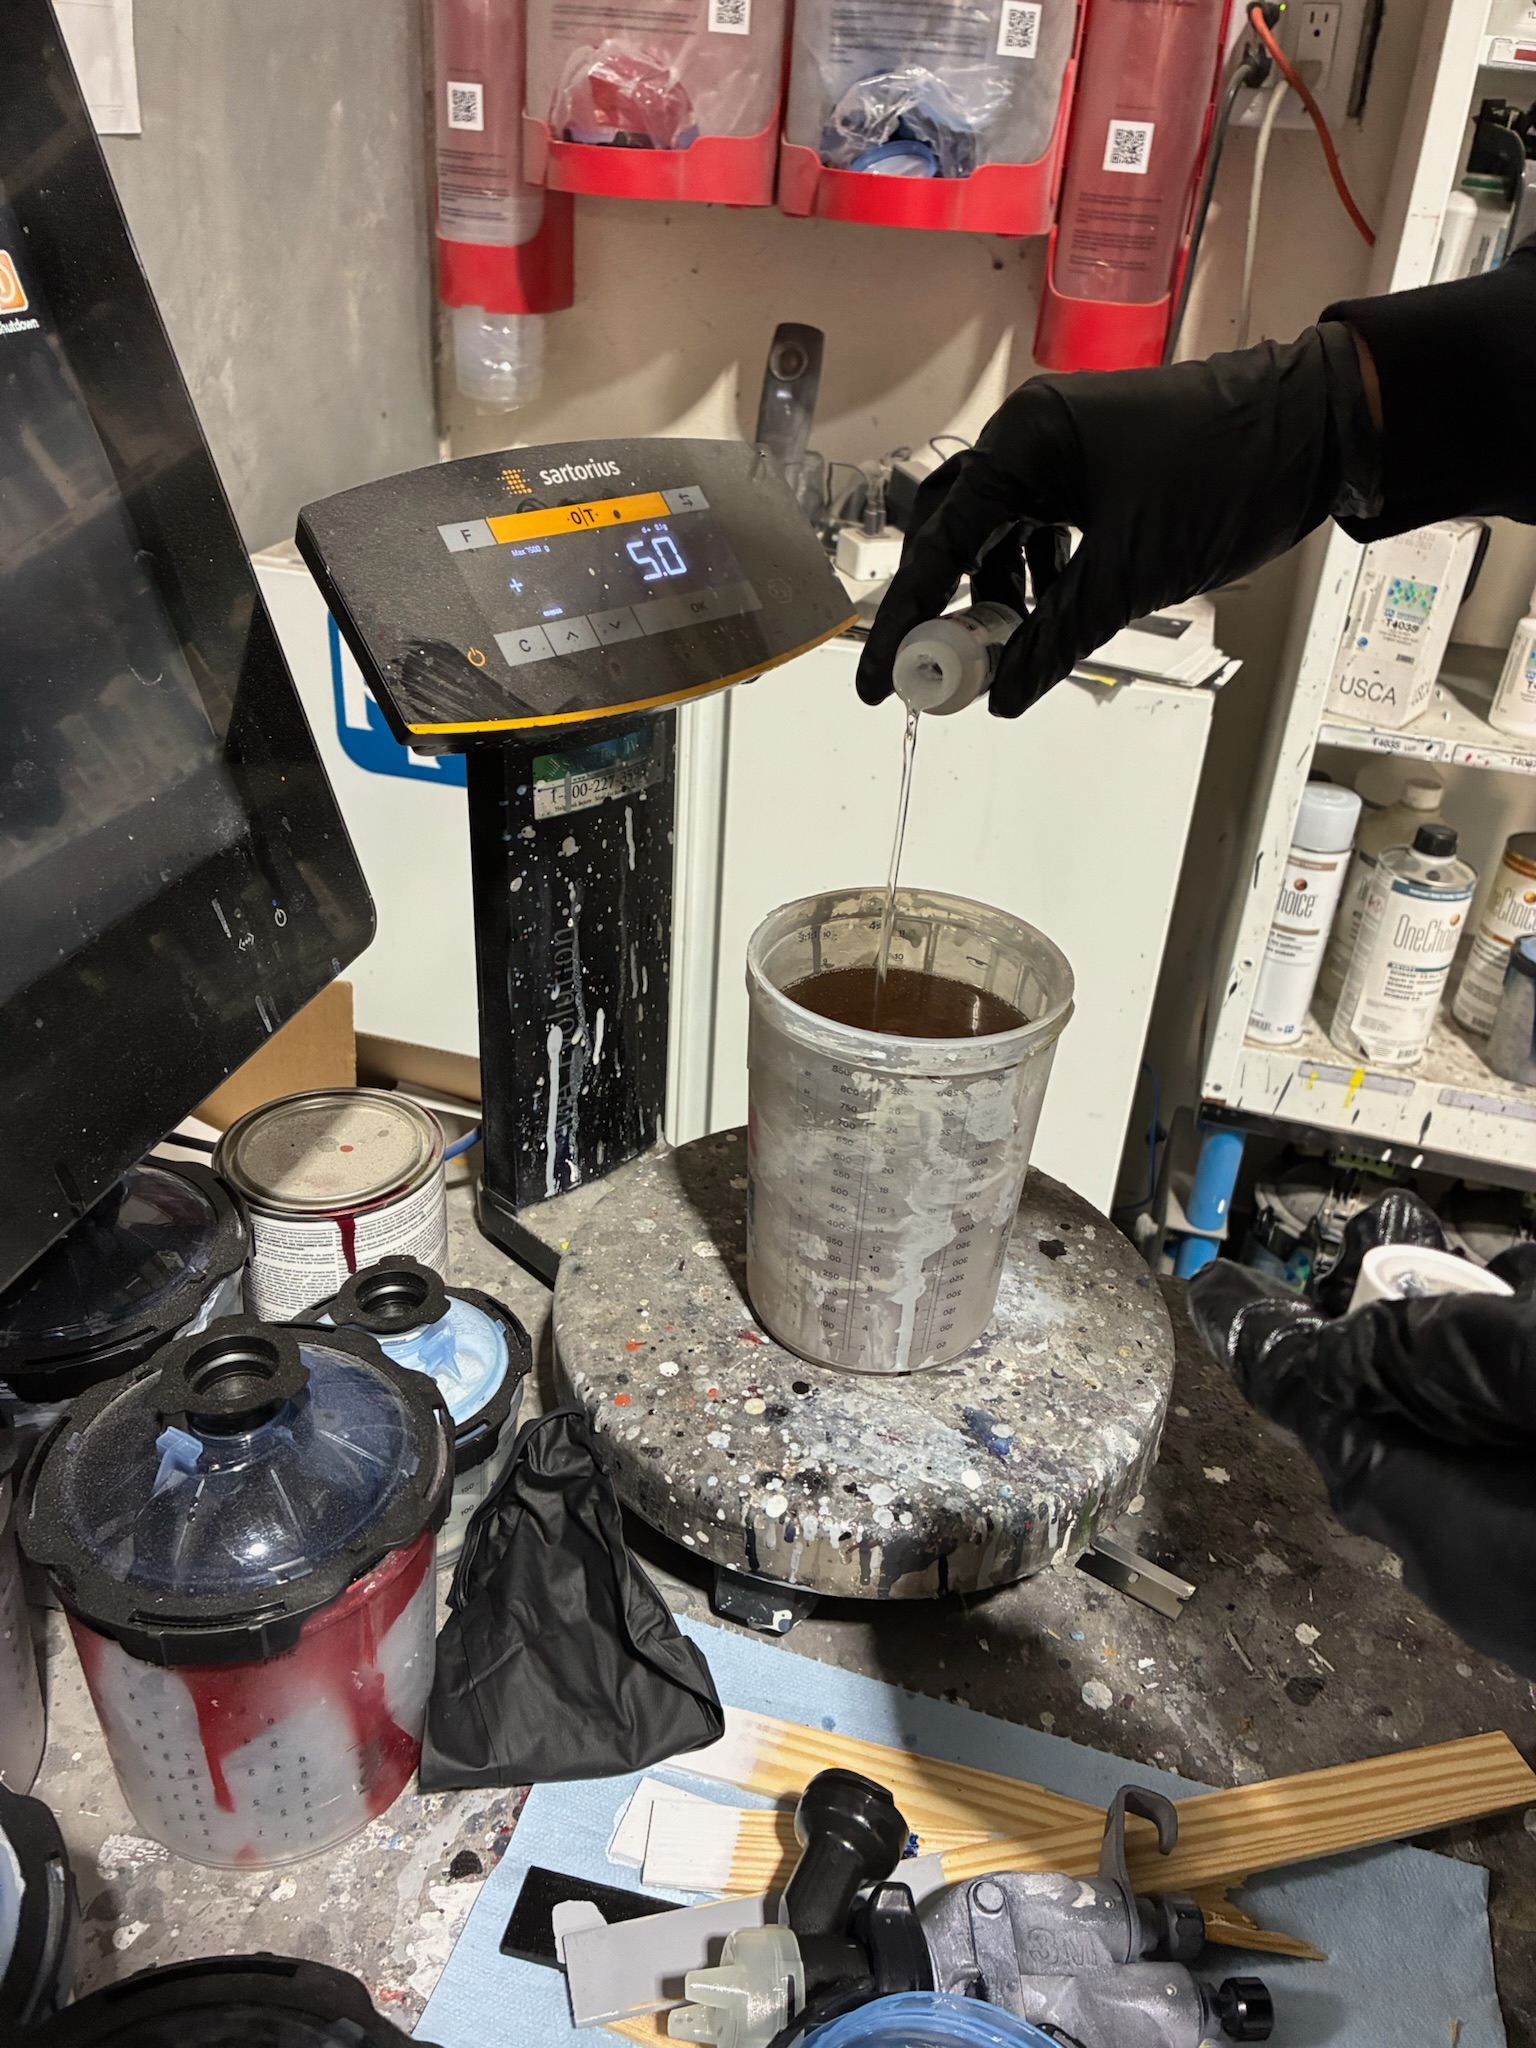
\includegraphics[
        width=2.35in,
        height=1.40in,
        keepaspectratio
    ]{spray_topcoat_prep}
};
\draw[RuleGray,line width=0.55pt,rounded corners=4pt]
    ($(current page.north west)+(0.43in,-1.91in)$)
    rectangle
    ($(current page.north west)+(2.98in,-3.40in)$);

% Image 2
\node[anchor=center,inner sep=0pt]
at ($(current page.north west)+(4.375in,-2.655in)$)
{
    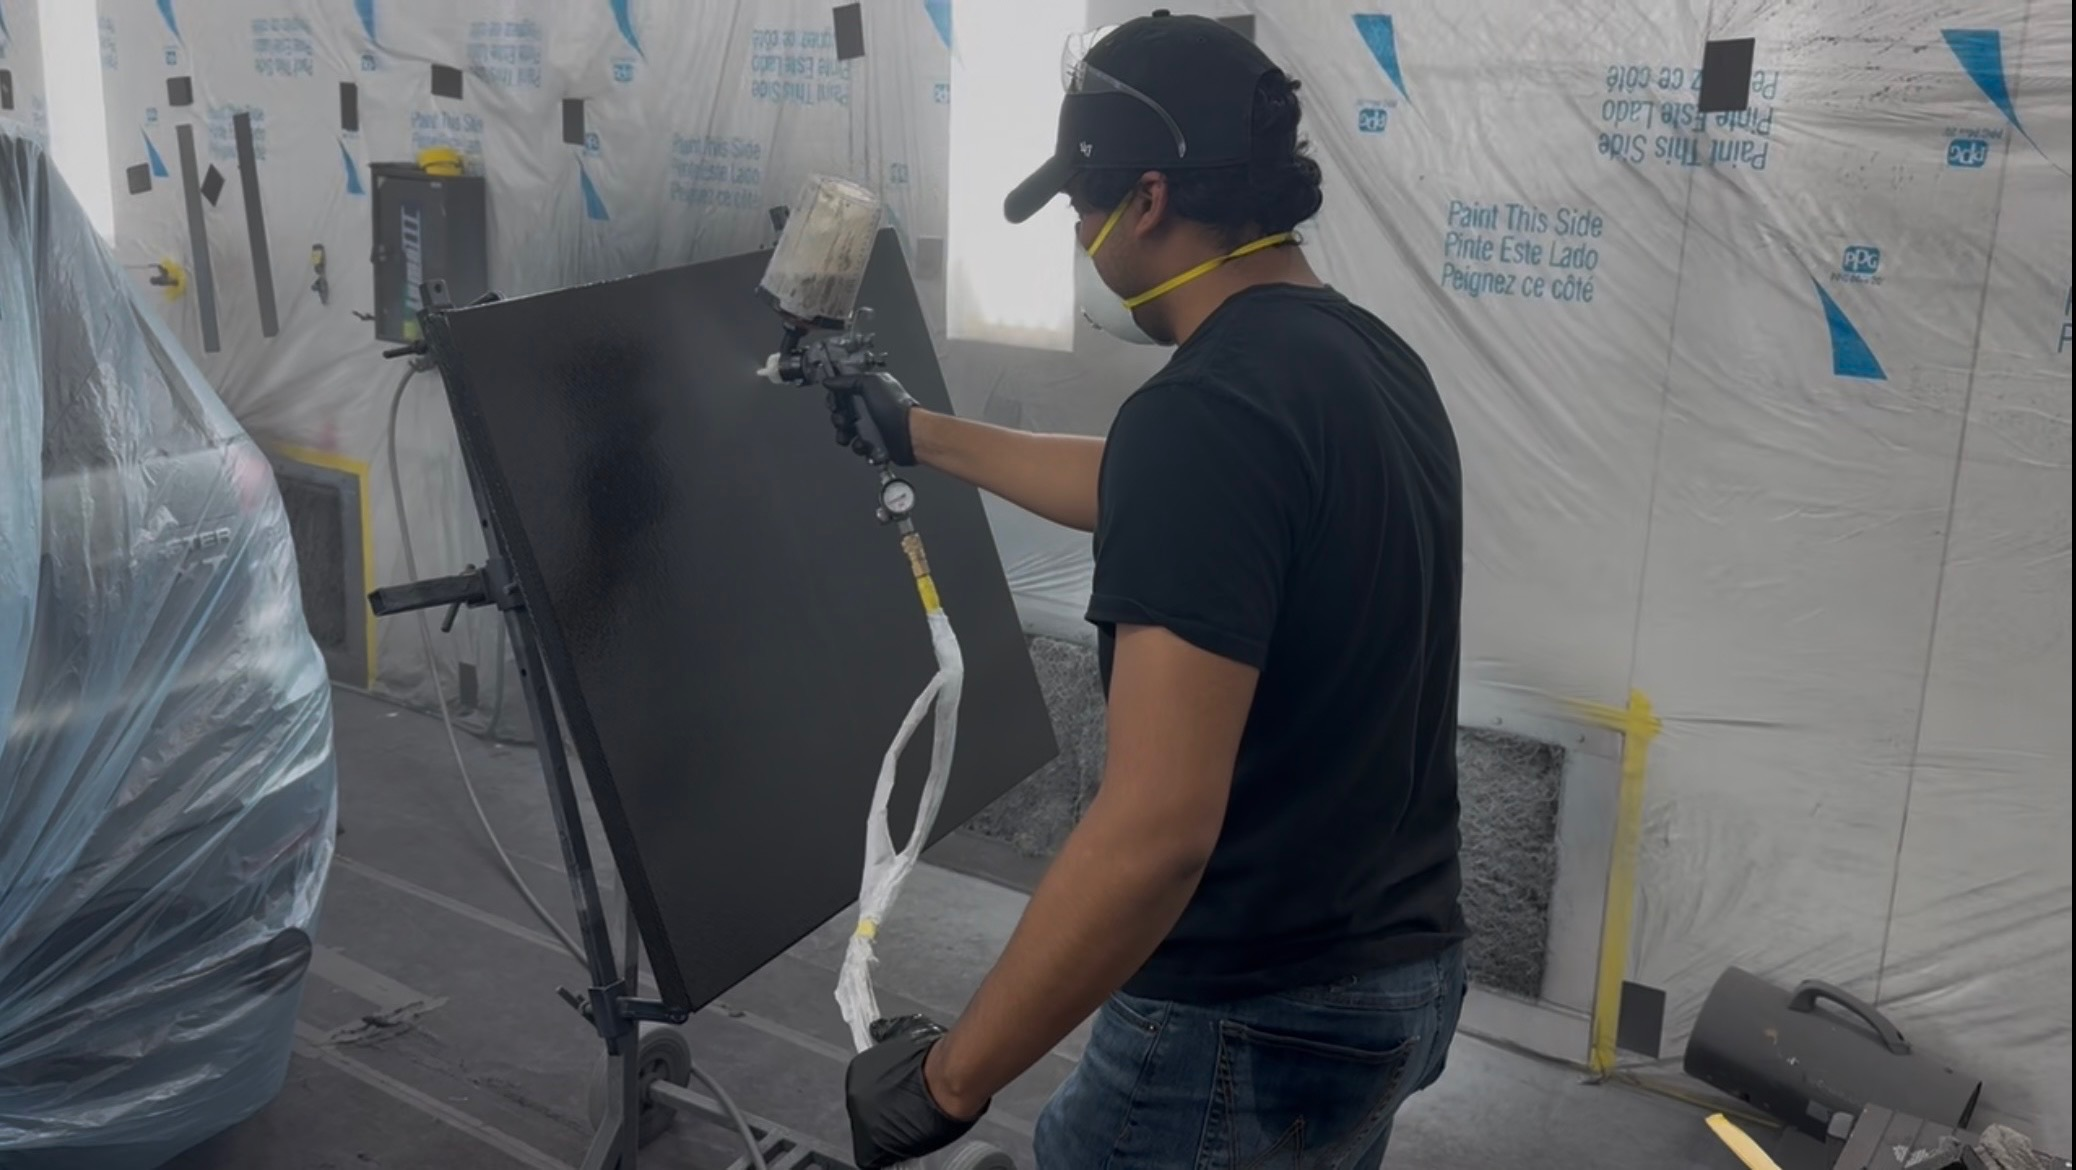
\includegraphics[
        width=2.35in,
        height=1.40in,
        keepaspectratio
    ]{spraying_topcoat}
};
\draw[RuleGray,line width=0.55pt,rounded corners=4pt]
    ($(current page.north west)+(3.10in,-1.91in)$)
    rectangle
    ($(current page.north west)+(5.65in,-3.40in)$);

% Image 3
\node[anchor=center,inner sep=0pt]
at ($(current page.north west)+(7.045in,-2.655in)$)
{
    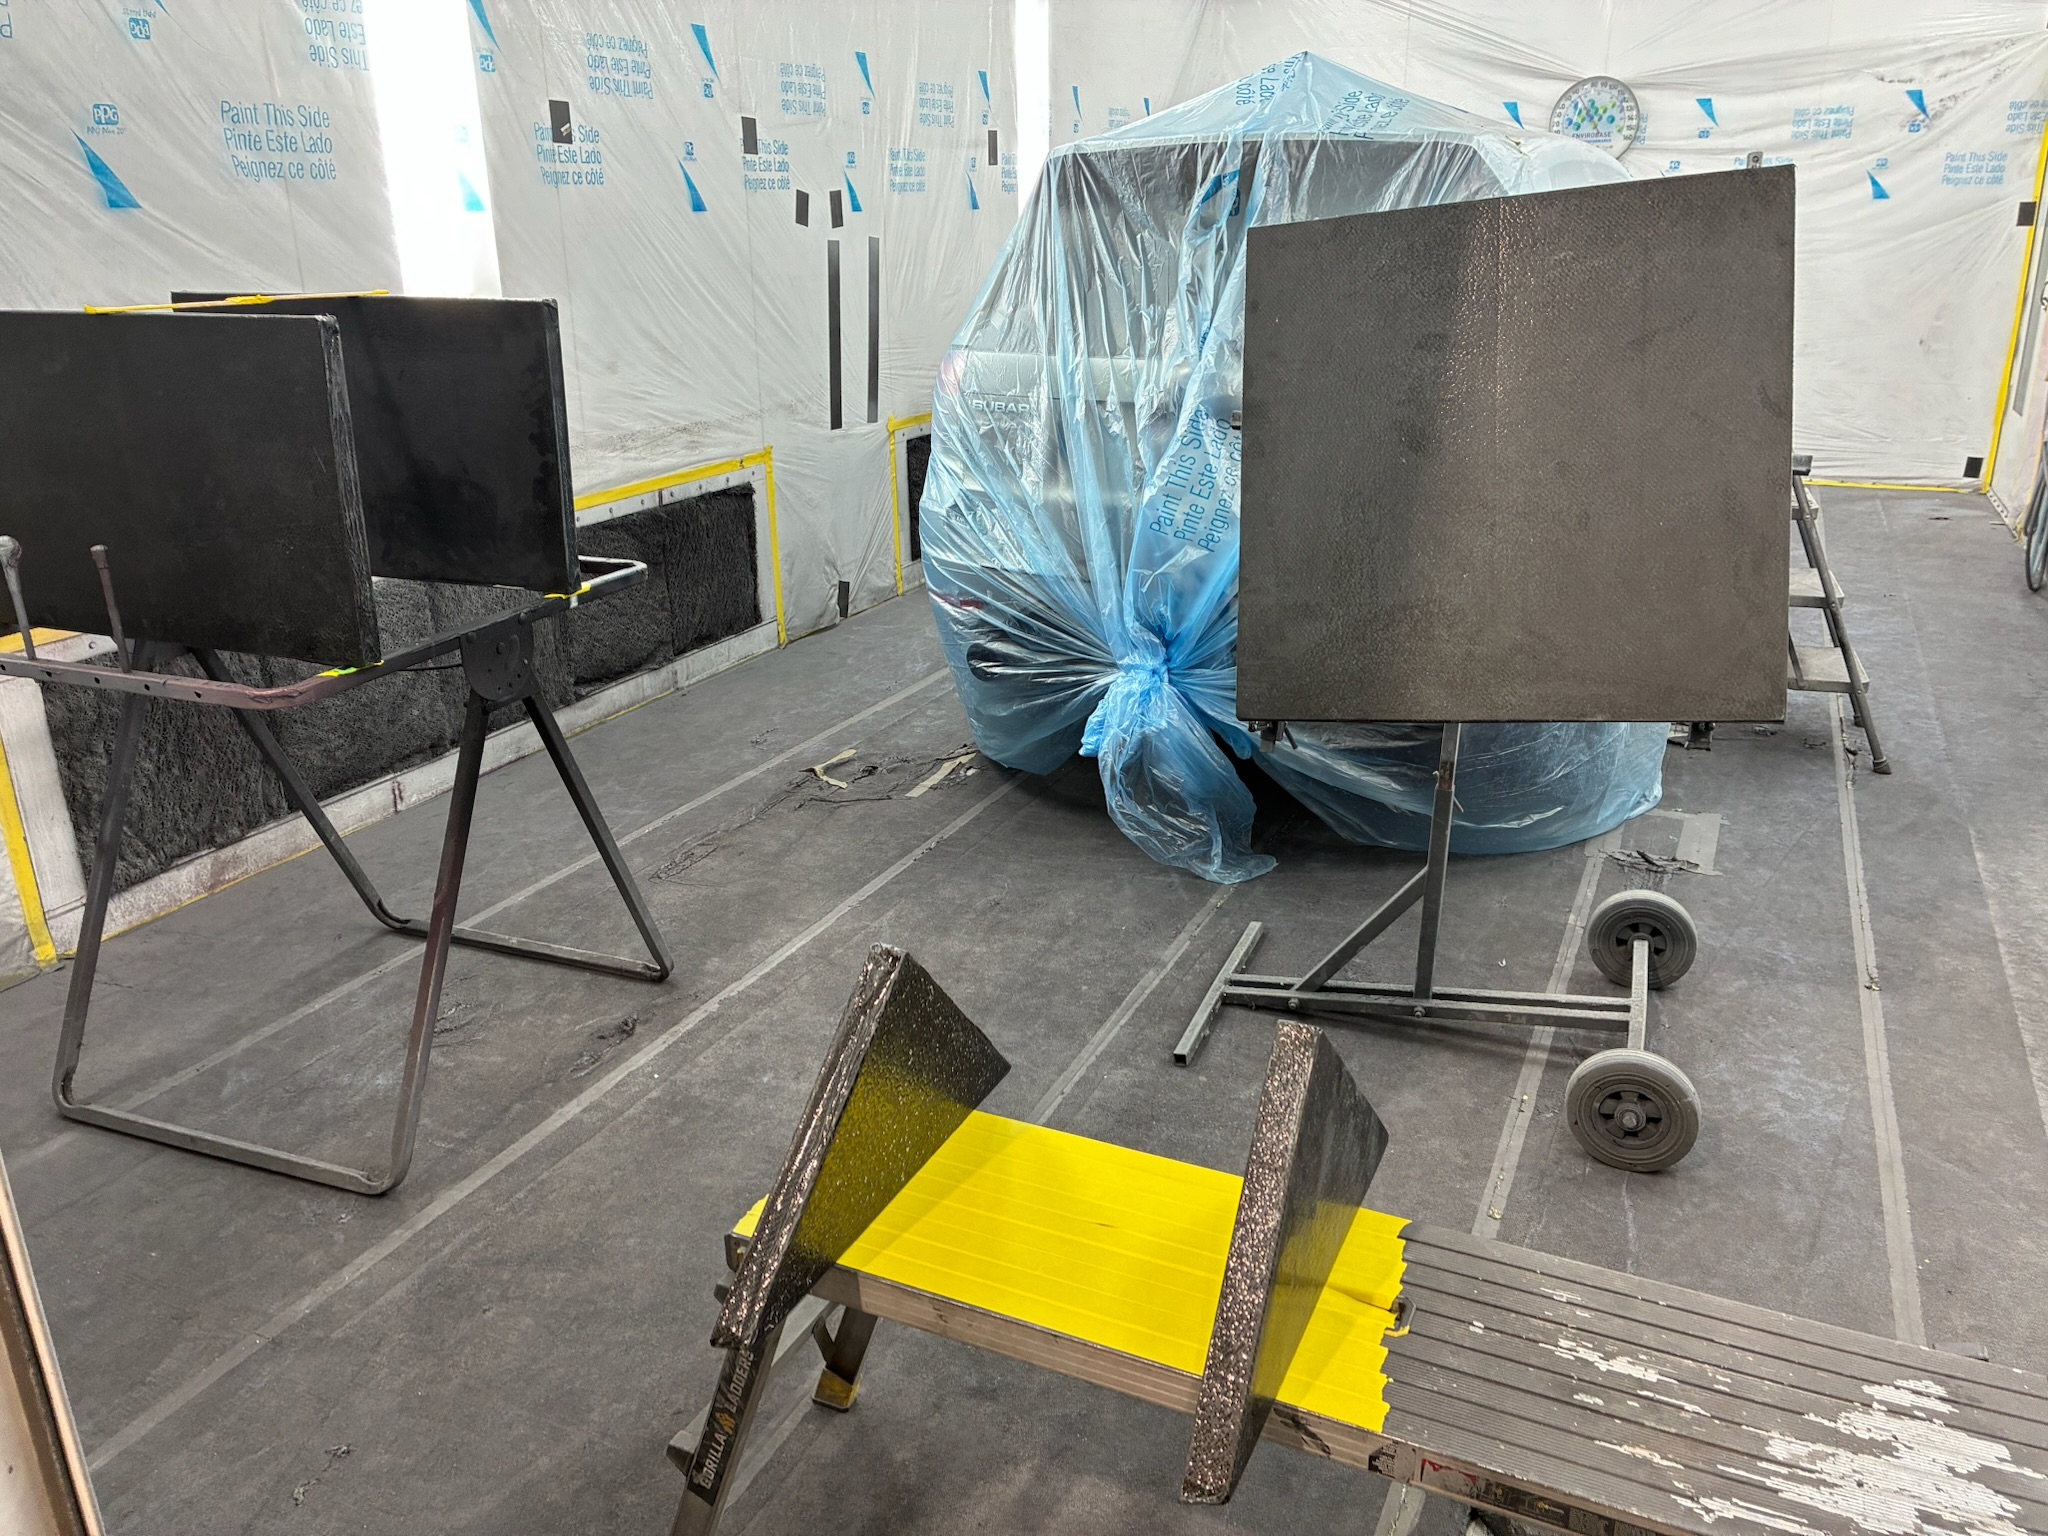
\includegraphics[
        width=2.35in,
        height=1.40in,
        keepaspectratio
    ]{topcoat_setup_apparatus}
};
\draw[RuleGray,line width=0.55pt,rounded corners=4pt]
    ($(current page.north west)+(5.77in,-1.91in)$)
    rectangle
    ($(current page.north west)+(8.32in,-3.40in)$);

% Image 4
\node[anchor=center,inner sep=0pt]
at ($(current page.north west)+(9.50in,-2.655in)$)
{
    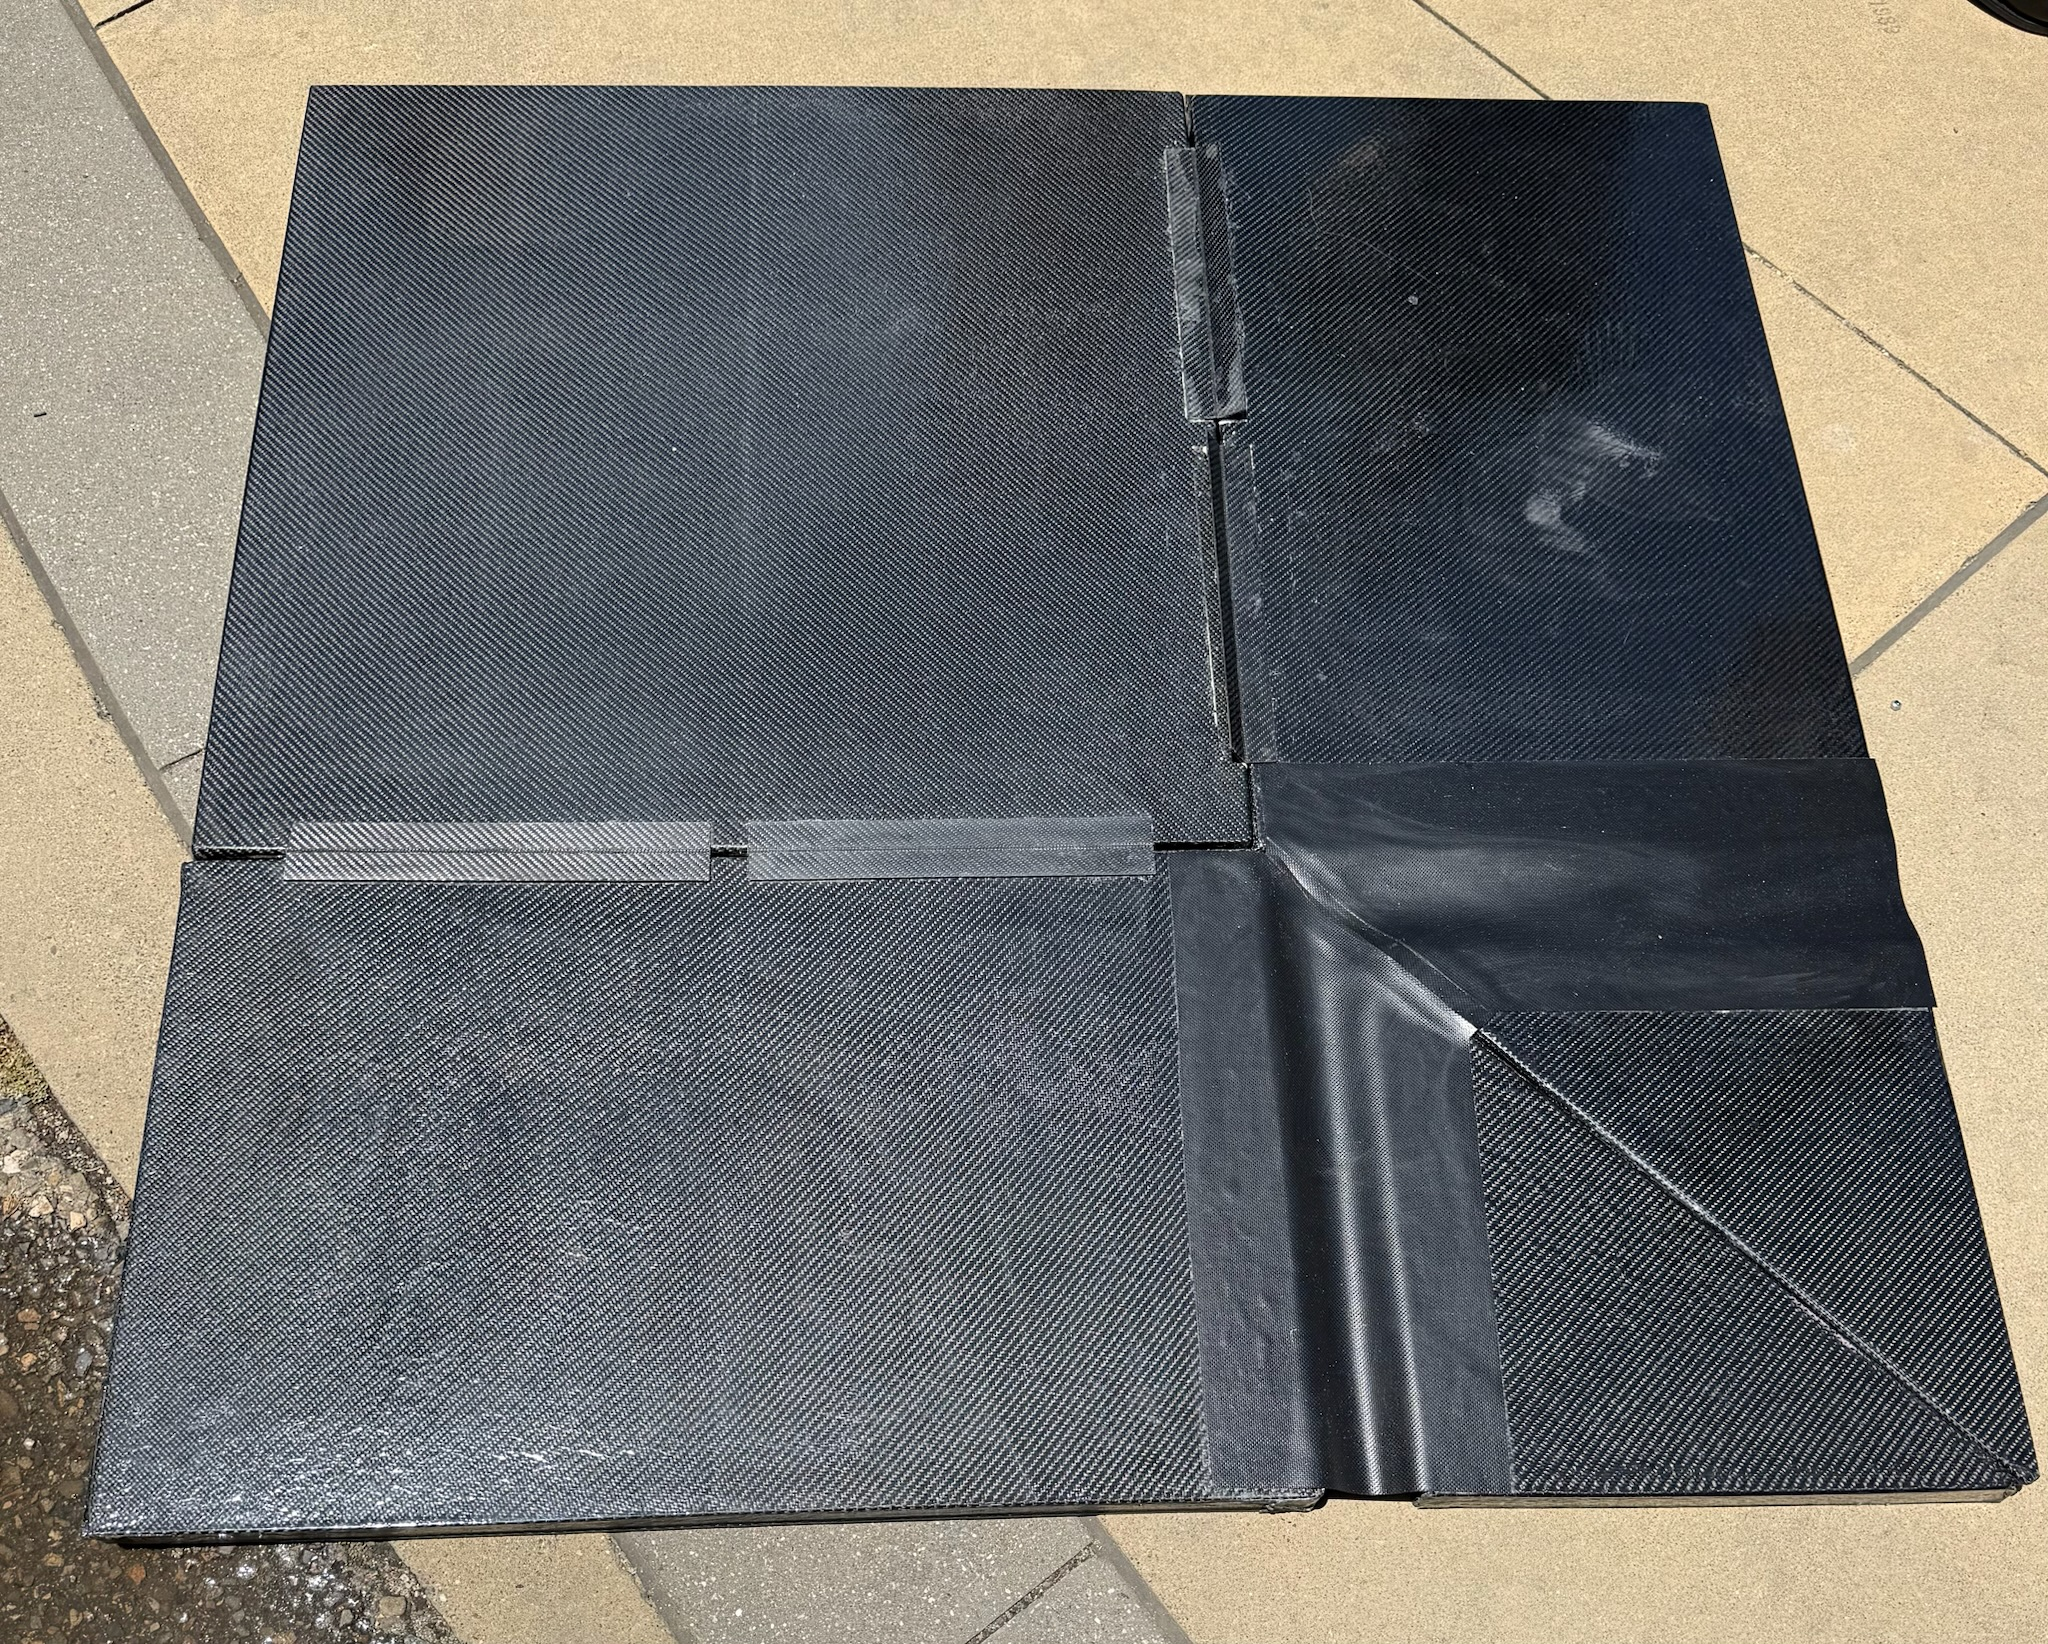
\includegraphics[
        width=2.35in,
        height=1.40in,
        keepaspectratio
    ]{refined_final_toro_cover_partial_carbon_model}
};
\draw[RuleGray,line width=0.55pt,rounded corners=4pt]
    ($(current page.north west)+(8.44in,-1.91in)$)
    rectangle
    ($(current page.north east)+(-0.42in,-3.40in)$);

% Captions
\node[anchor=north,text=Muted,font=\sffamily\fontsize{6.7}{7.3}\selectfont]
at ($(current page.north west)+(1.705in,-3.45in)$)
{Topcoat material preparation};

\node[anchor=north,text=Muted,font=\sffamily\fontsize{6.7}{7.3}\selectfont]
at ($(current page.north west)+(4.375in,-3.45in)$)
{Automotive-booth topcoat application};

\node[anchor=north,text=Muted,font=\sffamily\fontsize{6.7}{7.3}\selectfont]
at ($(current page.north west)+(7.045in,-3.45in)$)
{Coated panels drying after application};

\node[anchor=north,text=Muted,font=\sffamily\fontsize{6.7}{7.3}\selectfont]
at ($(current page.north west)+(9.50in,-3.45in)$)
{Partial carbon manufacturing model};

% Environmental rationale
\fill[SoftGold,rounded corners=4pt]
    ($(current page.north west)+(0.43in,-3.73in)$)
    rectangle
    ($(current page.north east)+(-0.42in,-4.76in)$);

\node[
    anchor=north west,
    align=left,
    text width=9.75in,
    text=Ink,
    font=\fontsize{7.05}{8.25}\selectfont
]
at ($(current page.north west)+(0.65in,-3.89in)$)
{
Because the sponsor required a carbon-fiber cover for outdoor use near chlorinated water,
environmental protection became a functional requirement rather than a cosmetic finish.
I selected and personally sprayed a UV-resistant Sunshield topcoat to seal minor laminate
porosity, reduce moisture ingress, preserve the carbon appearance, limit UV degradation of
the epoxy matrix, and isolate the composite surface from nearby metallic hardware.
};

% Results title
\node[
    anchor=north west,
    text=DeepGreen,
    font=\sffamily\bfseries\fontsize{8.0}{8.7}\selectfont
]
at ($(current page.north west)+(0.43in,-4.94in)$)
{FUNCTIONAL PROTOTYPE RESULTS};

% ------------------------------------------------------------
% Matched lower panels — larger type and improved allocation
% ------------------------------------------------------------

% Left results panel
\fill[SoftGreen,rounded corners=5pt]
    ($(current page.north west)+(0.43in,-5.22in)$)
    rectangle
    ($(current page.north west)+(5.98in,-7.39in)$);

\draw[RuleGray,line width=0.65pt,rounded corners=5pt]
    ($(current page.north west)+(0.43in,-5.22in)$)
    rectangle
    ($(current page.north west)+(5.98in,-7.39in)$);

\fill[DeepGreen,rounded corners=5pt]
    ($(current page.north west)+(0.43in,-5.22in)$)
    rectangle
    ($(current page.north west)+(5.98in,-5.58in)$);

\fill[DeepGreen]
    ($(current page.north west)+(0.43in,-5.40in)$)
    rectangle
    ($(current page.north west)+(5.98in,-5.58in)$);

\node[anchor=west,text=white,
      font=\sffamily\bfseries\fontsize{7.0}{7.6}\selectfont]
at ($(current page.north west)+(0.66in,-5.40in)$)
{SPECIFICATION};

\node[anchor=west,text=white,
      font=\sffamily\bfseries\fontsize{7.0}{7.6}\selectfont]
at ($(current page.north west)+(3.02in,-5.40in)$)
{RESULT};

\node[anchor=east,text=white,
      font=\sffamily\bfseries\fontsize{7.0}{7.6}\selectfont]
at ($(current page.north west)+(5.55in,-5.40in)$)
{STATUS};

\node[
    anchor=north west,
    align=left,
    text width=2.15in,
    text=Ink,
    font=\bfseries\fontsize{7.15}{8.55}\selectfont
]
at ($(current page.north west)+(0.66in,-5.72in)$)
{
Deployment time\\[3.4pt]
Removal time\\[3.4pt]
Single-user operation\\[3.4pt]
Single-side operation\\[3.4pt]
Deployment steps\\[3.4pt]
Removal steps\\[3.4pt]
Weight\\[3.4pt]
Folded storage
};

\node[
    anchor=north west,
    align=left,
    text width=1.45in,
    text=Ink,
    font=\fontsize{7.15}{8.55}\selectfont
]
at ($(current page.north west)+(3.02in,-5.72in)$)
{
25.51 seconds\\[3.4pt]
37.22 seconds\\[3.4pt]
100\% successful\\[3.4pt]
75\% successful\\[3.4pt]
6.4 average\\[3.4pt]
9 average\\[3.4pt]
17 lb\\[3.4pt]
2.9' x 2.9' x 1.7'
};

\node[
    anchor=north east,
    align=right,
    text width=1.05in,
    text=DeepGreen,
    font=\sffamily\bfseries\fontsize{7.05}{8.55}\selectfont
]
at ($(current page.north west)+(5.55in,-5.72in)$)
{
PASS\\[3.4pt]
PASS\\[3.4pt]
PASS\\[3.4pt]
NEAR TARGET\\[3.4pt]
PASS\\[3.4pt]
PASS\\[3.4pt]
NEAR TARGET\\[3.4pt]
PASS
};

% Right takeaways panel — widened for easier reading
\fill[SoftGreen,rounded corners=5pt]
    ($(current page.north west)+(6.14in,-5.22in)$)
    rectangle
    ($(current page.north east)+(-0.42in,-7.39in)$);

\draw[RuleGray,line width=0.65pt,rounded corners=5pt]
    ($(current page.north west)+(6.14in,-5.22in)$)
    rectangle
    ($(current page.north east)+(-0.42in,-7.39in)$);

\fill[DeepGreen,rounded corners=5pt]
    ($(current page.north west)+(6.14in,-5.22in)$)
    rectangle
    ($(current page.north east)+(-0.42in,-5.58in)$);

\fill[DeepGreen]
    ($(current page.north west)+(6.14in,-5.40in)$)
    rectangle
    ($(current page.north east)+(-0.42in,-5.58in)$);

\node[anchor=west,text=white,
      font=\sffamily\bfseries\fontsize{7.1}{7.7}\selectfont]
at ($(current page.north west)+(6.38in,-5.40in)$)
{ENGINEERING TAKEAWAYS};

\node[
    anchor=north west,
    align=left,
    text width=4.02in,
    text=Ink,
    font=\fontsize{6.75}{7.85}\selectfont
]
at ($(current page.north west)+(6.38in,-5.72in)$)
{
\textbf{Manufacturing first.}
Composite manufacturing constraints should guide the product architecture from the beginning.\\[4.5pt]
\textbf{Prioritize deliberately.}
Competing requirements must be balanced intentionally instead of maximizing every objective.\\[4.5pt]
\textbf{Lead through the process.}
Clear procedures, calm communication, and respect for teammates' strengths were essential during fabrication.\\[4.5pt]
\textbf{Next iteration.}
Reduce weight, refine the fabric-hinge fold lines, and improve panel-edge clearance.
};

% Compact concluding pathway
\node[
    anchor=center,
    align=center,
    text=PolyGold,
    font=\sffamily\bfseries\fontsize{6.3}{6.9}\selectfont
]
at ($(current page.north)+(3.06in,-7.18in)$)
{PROTOTYPE \faArrowRight\ DESIGN REFINEMENT
\faArrowRight\ REPEATABLE MANUFACTURING
\faArrowRight\ PRODUCT};

% Validation resources
\node[
    anchor=north,
    align=center,
    text=DeepGreen,
    font=\sffamily\bfseries\fontsize{6.6}{7.2}\selectfont
]
at ($(current page.north)+(0,-7.58in)$)
{\href{\ToroDeploymentLink}{\faPlayCircle\ DEPLOYMENT}
\hspace{18pt}
\href{\ToroRemovalLink}{\faPlayCircle\ REMOVAL / FOLDING}
\hspace{18pt}
\href{\ToroPosterLink}{\faFilePdf\ EXPO POSTER}
\hspace{18pt}
\href{\ToroReportLink}{\faFilePdf\ FINAL REPORT}};

% Footer
\node[
    anchor=south west,
    text=white,
    font=\sffamily\bfseries\fontsize{7.1}{7.7}\selectfont
]
at ($(current page.south west)+(0.42in,0.17in)$)
{\faArrowLeft\ MANUFACTURING-DRIVEN DESIGN};

\node[
    anchor=south,
    text=white,
    font=\sffamily\fontsize{7.0}{7.6}\selectfont
]
at ($(current page.south)+(0,0.17in)$)
{TORO COVER \hspace{6pt} 3 / 3};

\node[
    anchor=south east,
    text=white,
    font=\sffamily\bfseries\fontsize{7.1}{7.7}\selectfont
]
at ($(current page.south east)+(-0.42in,0.17in)$)
{NEXT PROJECT \faArrowRight};

\end{tikzpicture}

% ============================================================
% PICKLEBALL PADDLE — SINGLE-PAGE PORTFOLIO CASE STUDY
% Project 02 in the Composites section
%
% IMPORTANT:
% 1. This file must NOT contain \documentclass, \begin{document},
%    or \end{document}.
% 2. In main.tex, place \input{pickleball} before \end{document}.
% 3. Image references use these Overleaf base filenames:
%       waterjet
%       side_core_view
%       full_assy
%       front_view
%       LAMINATE
% ============================================================

% Clickable project resource
\providecommand{\PaddleWaterjetVideo}
{https://drive.google.com/file/d/1mTuaE_g5mE2f7Nn3R5k7yFxqCWH_pvBh/view?usp=drive_link}

\clearpage
\thispagestyle{empty}
\hypertarget{pickleball}{}
\null

\begin{tikzpicture}[remember picture,overlay]

% ============================================================
% BACKGROUND AND PAGE BARS
% ============================================================

\fill[white]
    (current page.south west)
    rectangle
    (current page.north east);

\fill[DeepGreen]
    (current page.north west)
    rectangle
    ($(current page.north east)+(0,-0.095in)$);

\fill[PolyGold]
    ($(current page.north west)+(0,-0.095in)$)
    rectangle
    ($(current page.north east)+(0,-0.14in)$);

\fill[DeepGreen]
    (current page.south west)
    rectangle
    ($(current page.south east)+(0,0.36in)$);

\fill[PolyGold]
    ($(current page.south west)+(0,0.36in)$)
    rectangle
    ($(current page.south east)+(0,0.405in)$);

% ============================================================
% HEADER
% ============================================================

\node[
    anchor=north west,
    text=PolyGold,
    font=\sffamily\bfseries\fontsize{8.1}{8.7}\selectfont
]
at ($(current page.north west)+(0.42in,-0.39in)$)
{01 COMPOSITES \hspace{5pt}/\hspace{5pt} PROJECT 02};

\node[
    anchor=north west,
    text=DeepGreen,
    font=\bfseries\fontsize{22.5}{23.5}\selectfont
]
at ($(current page.north west)+(0.40in,-0.67in)$)
{CARBON FIBER PICKLEBALL PADDLE};

\node[
    anchor=north west,
    text=Muted,
    font=\sffamily\fontsize{8.4}{9.2}\selectfont
]
at ($(current page.north west)+(0.42in,-1.12in)$)
{Cal Poly Composites Laboratory \hspace{7pt}\textbullet\hspace{7pt}
Individual Project \hspace{7pt}\textbullet\hspace{7pt}
Spring 2026 \hspace{7pt}\textbullet\hspace{7pt}
San Luis Obispo, California};

\fill[PolyGold]
    ($(current page.north west)+(0.42in,-1.36in)$)
    rectangle
    ($(current page.north west)+(6.10in,-1.315in)$);

% ============================================================
% TOP LEFT — HERO PRODUCT IMAGE
% ============================================================

\node[
    anchor=center,
    inner sep=3pt,
    draw=DeepGreen,
    line width=0.75pt,
    rounded corners=6pt
]
at ($(current page.north west)+(1.60in,-3.20in)$)
{
    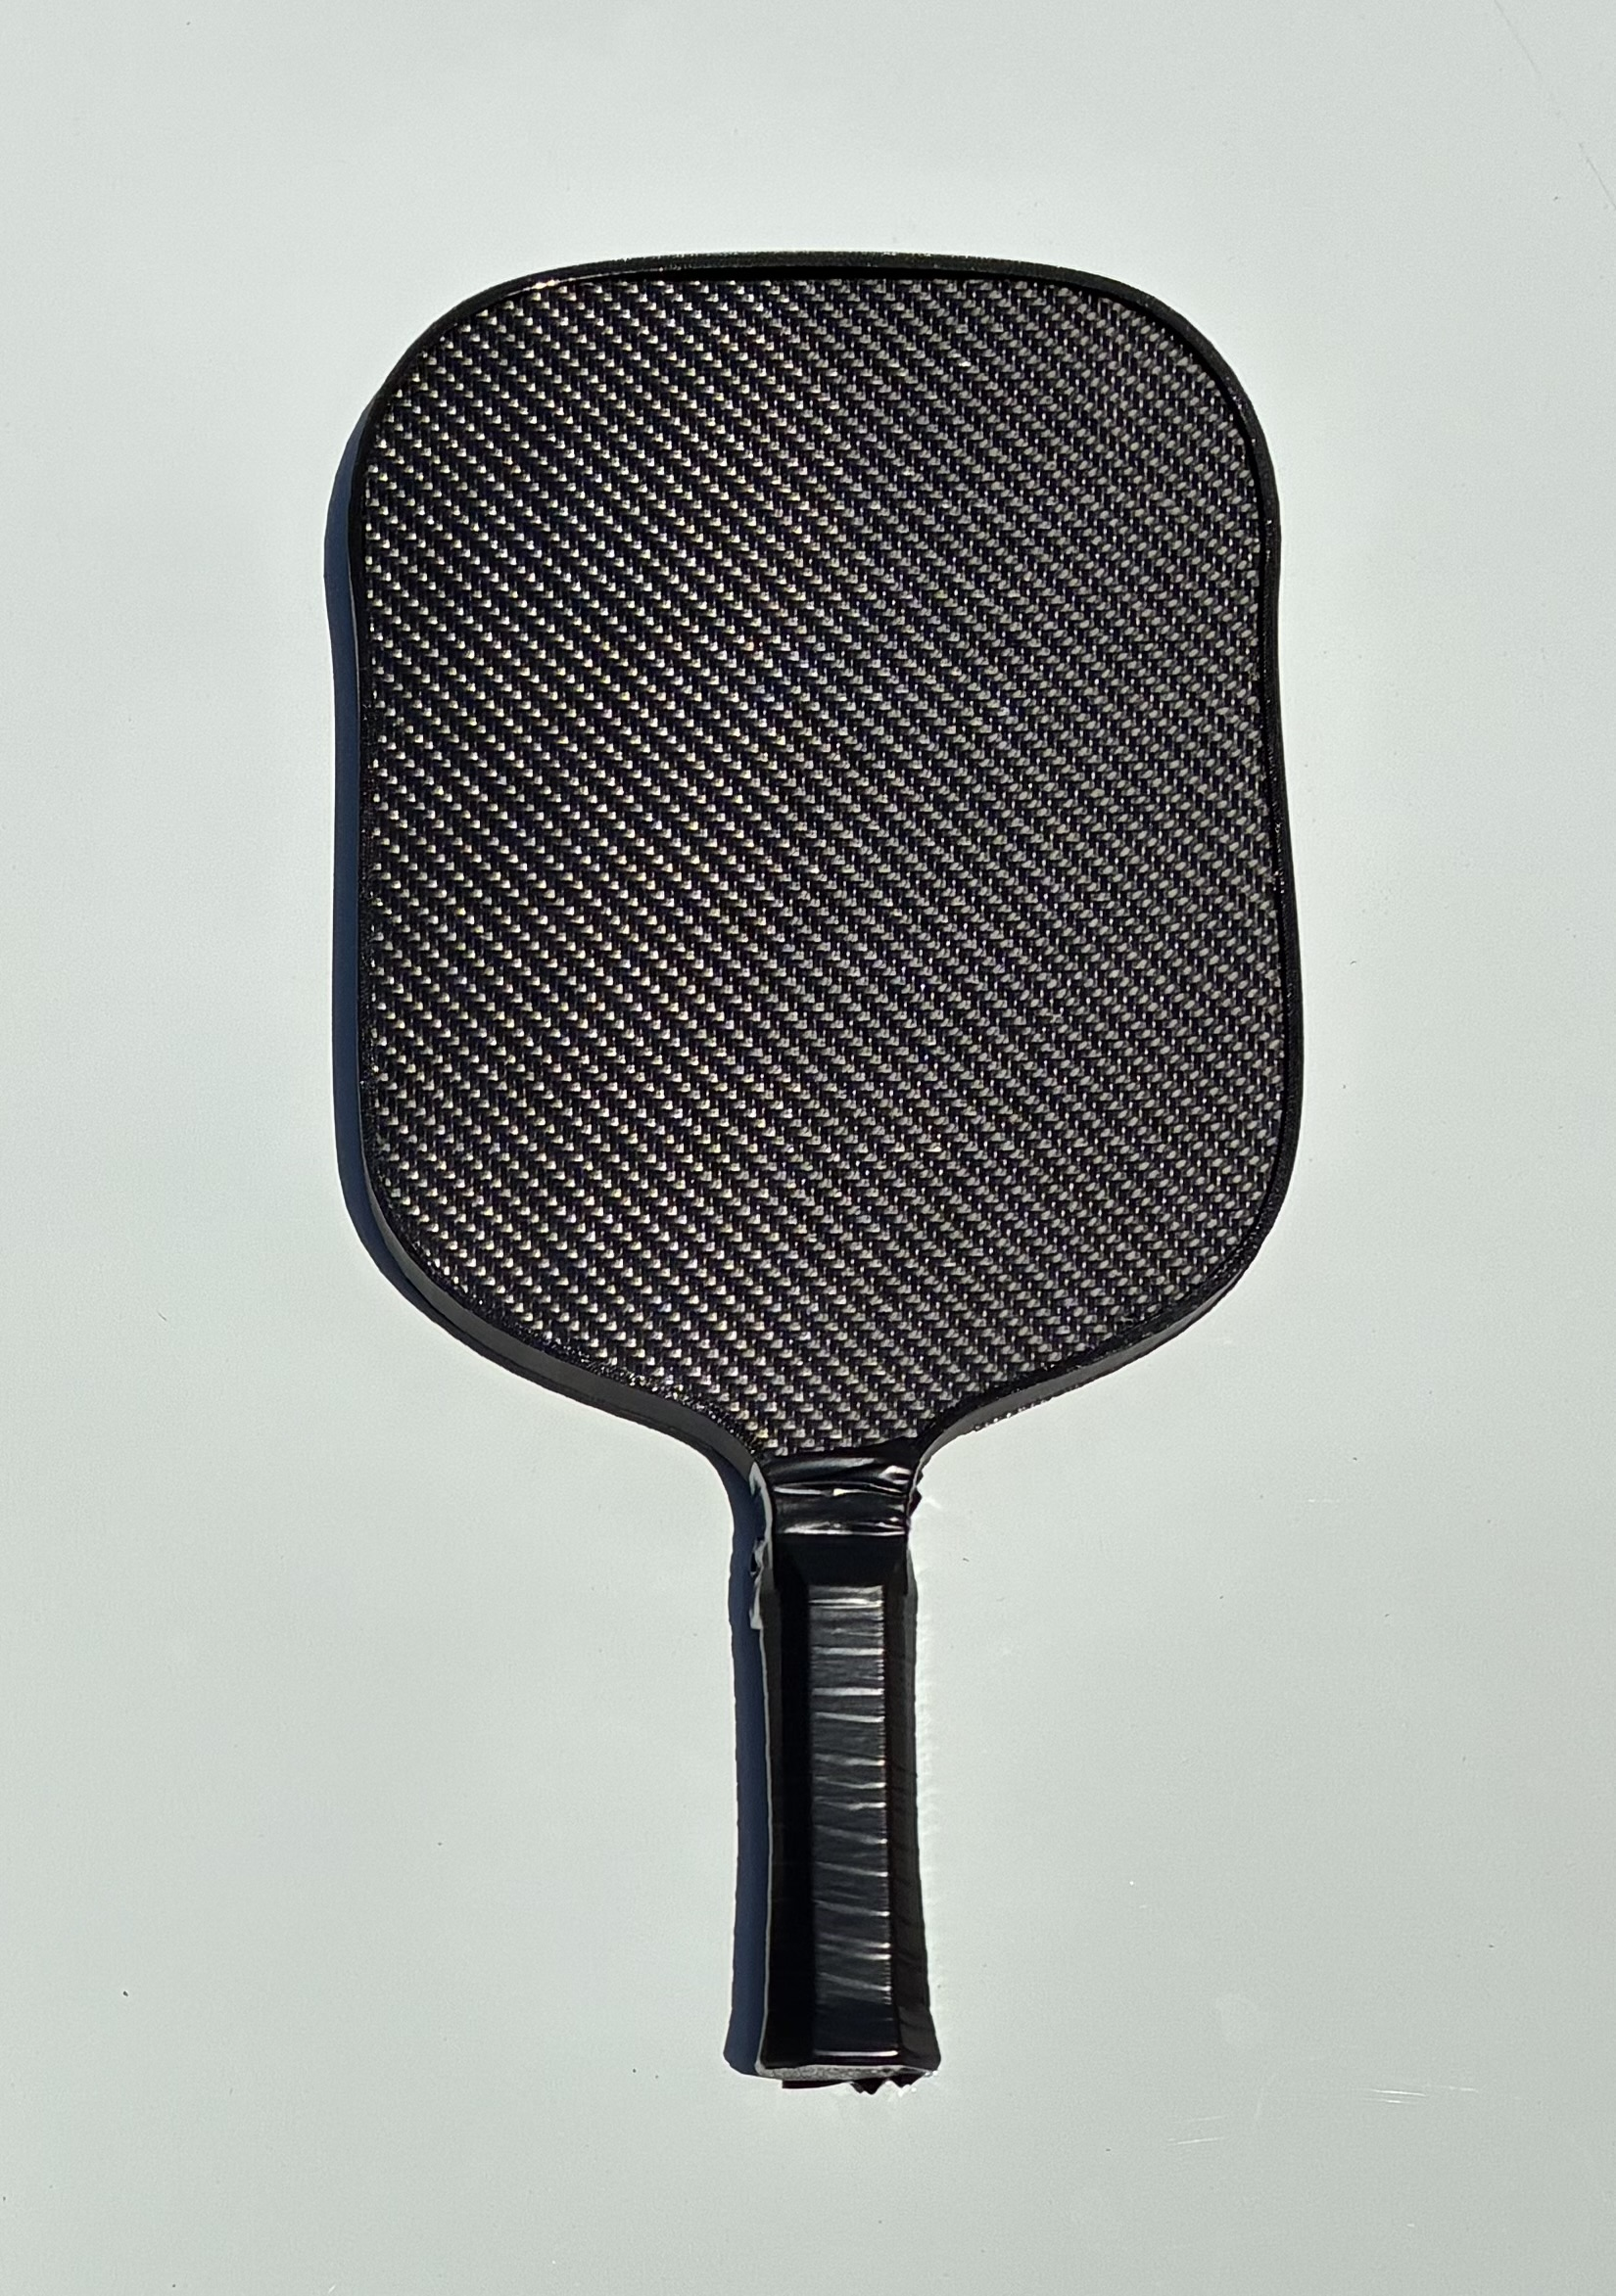
\includegraphics[
        width=3.72in,
        height=3.18in,
        keepaspectratio
    ]{full_assy}
};

\node[
    anchor=north,
    text=Muted,
    font=\sffamily\fontsize{6.9}{7.5}\selectfont
]
at ($(current page.north west)+(1.60in,-4.86in)$)
{Completed solo-built paddle assembly};

% ============================================================
% TOP CENTER — PROJECT OVERVIEW
% ============================================================

\fill[SoftGold,rounded corners=5pt]
    ($(current page.north west)+(2.95in,-1.62in)$)
    rectangle
    ($(current page.north west)+(5.53in,-4.86in)$);

\fill[PolyGold]
    ($(current page.north west)+(2.95in,-1.62in)$)
    rectangle
    ($(current page.north west)+(3.05in,-4.86in)$);

\node[
    anchor=north west,
    text=DeepGreen,
    font=\sffamily\bfseries\fontsize{8.0}{8.7}\selectfont
]
at ($(current page.north west)+(3.23in,-1.79in)$)
{PROJECT OVERVIEW};

\node[
    anchor=north west,
    align=left,
    text width=2.02in,
    text=Ink,
    font=\fontsize{7.05}{8.35}\selectfont
]
at ($(current page.north west)+(3.23in,-2.07in)$)
{
Independently designed and manufactured a lightweight prepreg
carbon-fiber pickleball paddle using a half-inch honeycomb
sandwich core, vacuum-bag consolidation, precision waterjet
trimming, and custom TPU and PLA components.

\vspace{5pt}

The project emphasized lightweight sandwich-composite design, repeatable manufacturing methods, dimensional accuracy, and the integration of custom 3D-printed TPU and PLA components into the final assembly.
};

\node[
    anchor=south west,
    align=left,
    text width=2.02in,
    text=PolyGold,
    font=\sffamily\bfseries\fontsize{6.65}{7.35}\selectfont
]
at ($(current page.north west)+(3.23in,-4.74in)$)
{
SOLE DESIGNER\\[2pt]
COMPOSITE FABRICATOR\\[2pt]
MANUFACTURING ENGINEER
};

% ============================================================
% TOP RIGHT — LAMINATE GRAPHIC
% ============================================================

\node[
    anchor=north west,
    inner sep=2.5pt,
    draw=DeepGreen,
    line width=0.65pt,
    rounded corners=5pt
]
at ($(current page.north west)+(5.71in,-1.62in)$)
{
    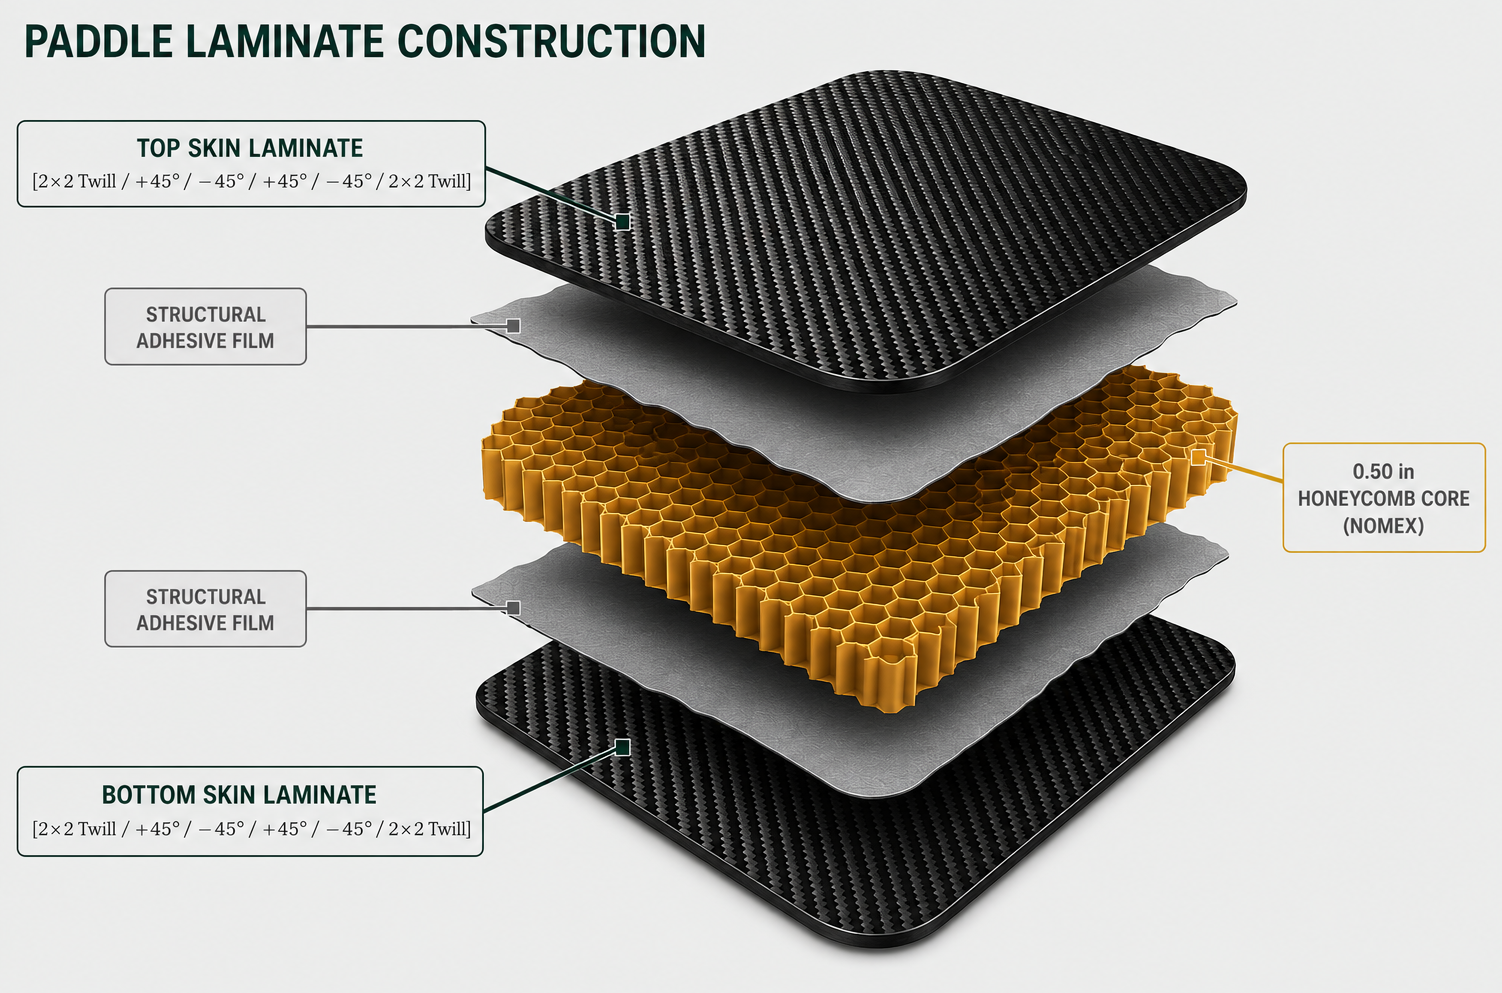
\includegraphics[
        width=4.80in,
        keepaspectratio
    ]{LAMINATE}
};

% ============================================================
% BOTTOM LEFT — SUPPORTING IMAGES
% ============================================================

\node[
    anchor=center,
    inner sep=3pt,
    draw=RuleGray,
    line width=0.55pt,
    rounded corners=4pt
]
at ($(current page.north west)+(1.12in,-5.98in)$)
{
    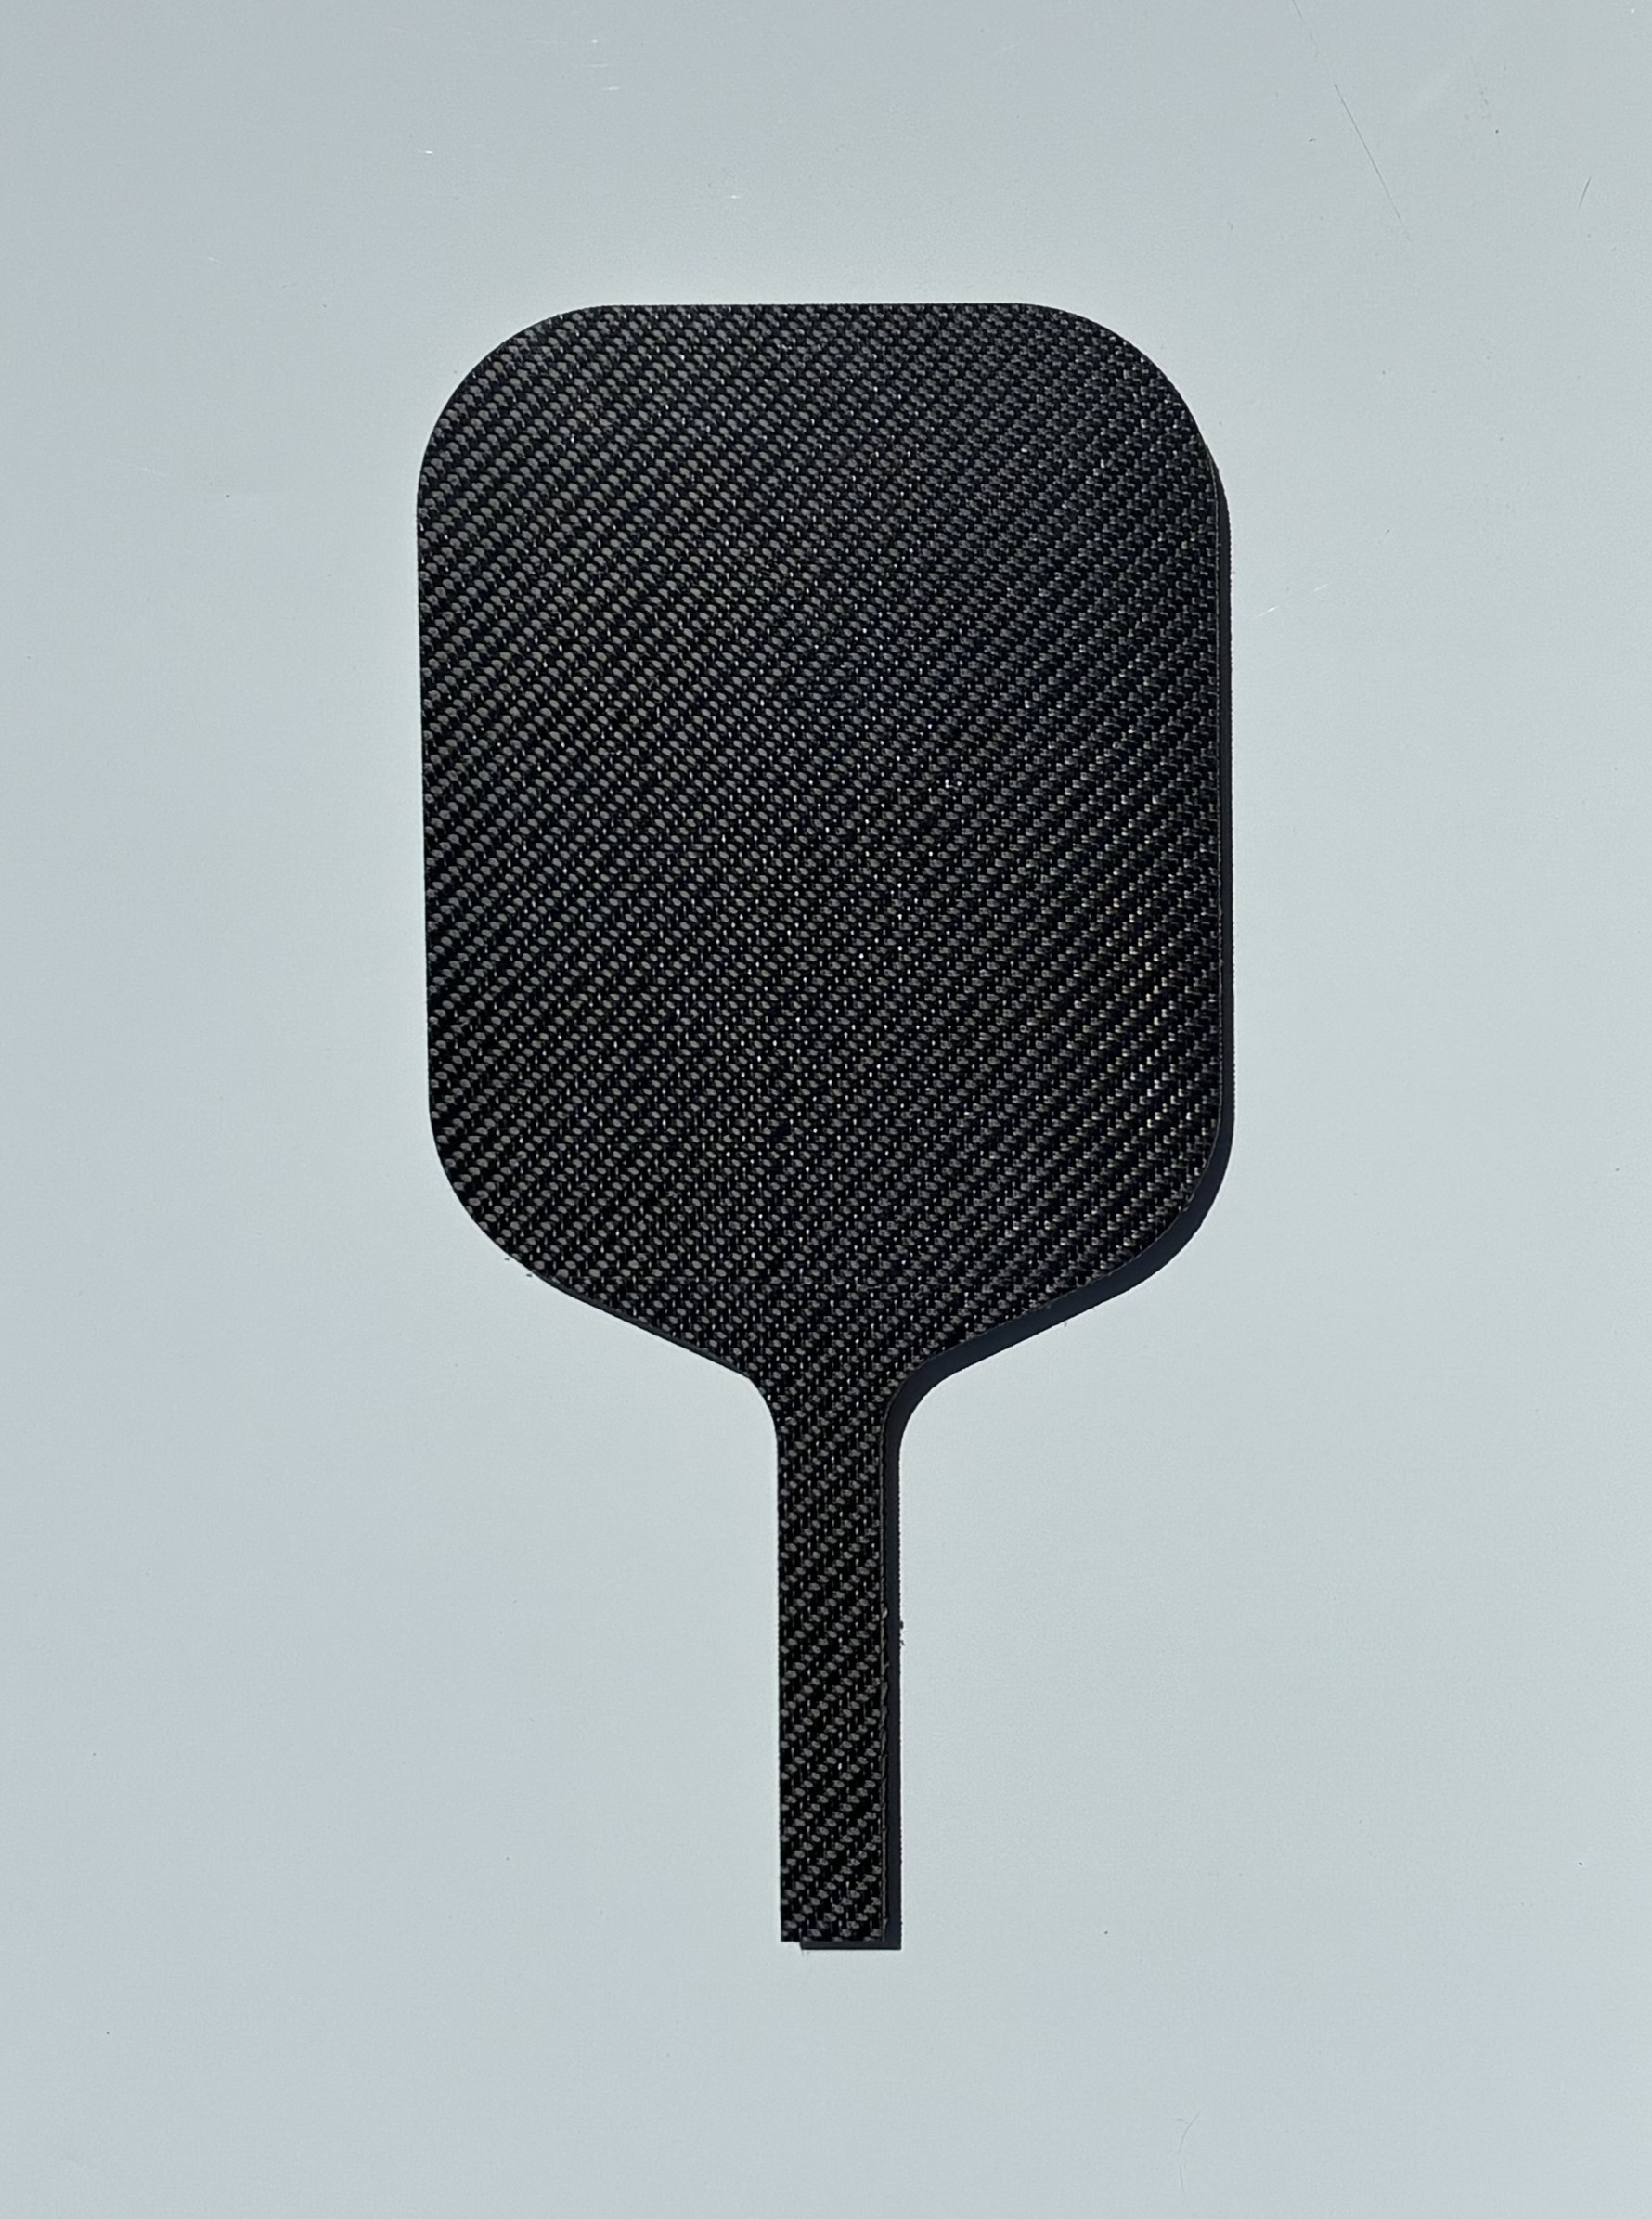
\includegraphics[
        width=1.30in,
        height=1.78in,
        keepaspectratio
    ]{front_view}
};

\node[
    anchor=center,
    inner sep=3pt,
    draw=RuleGray,
    line width=0.55pt,
    rounded corners=4pt
]
at ($(current page.north west)+(2.72in,-5.98in)$)
{
    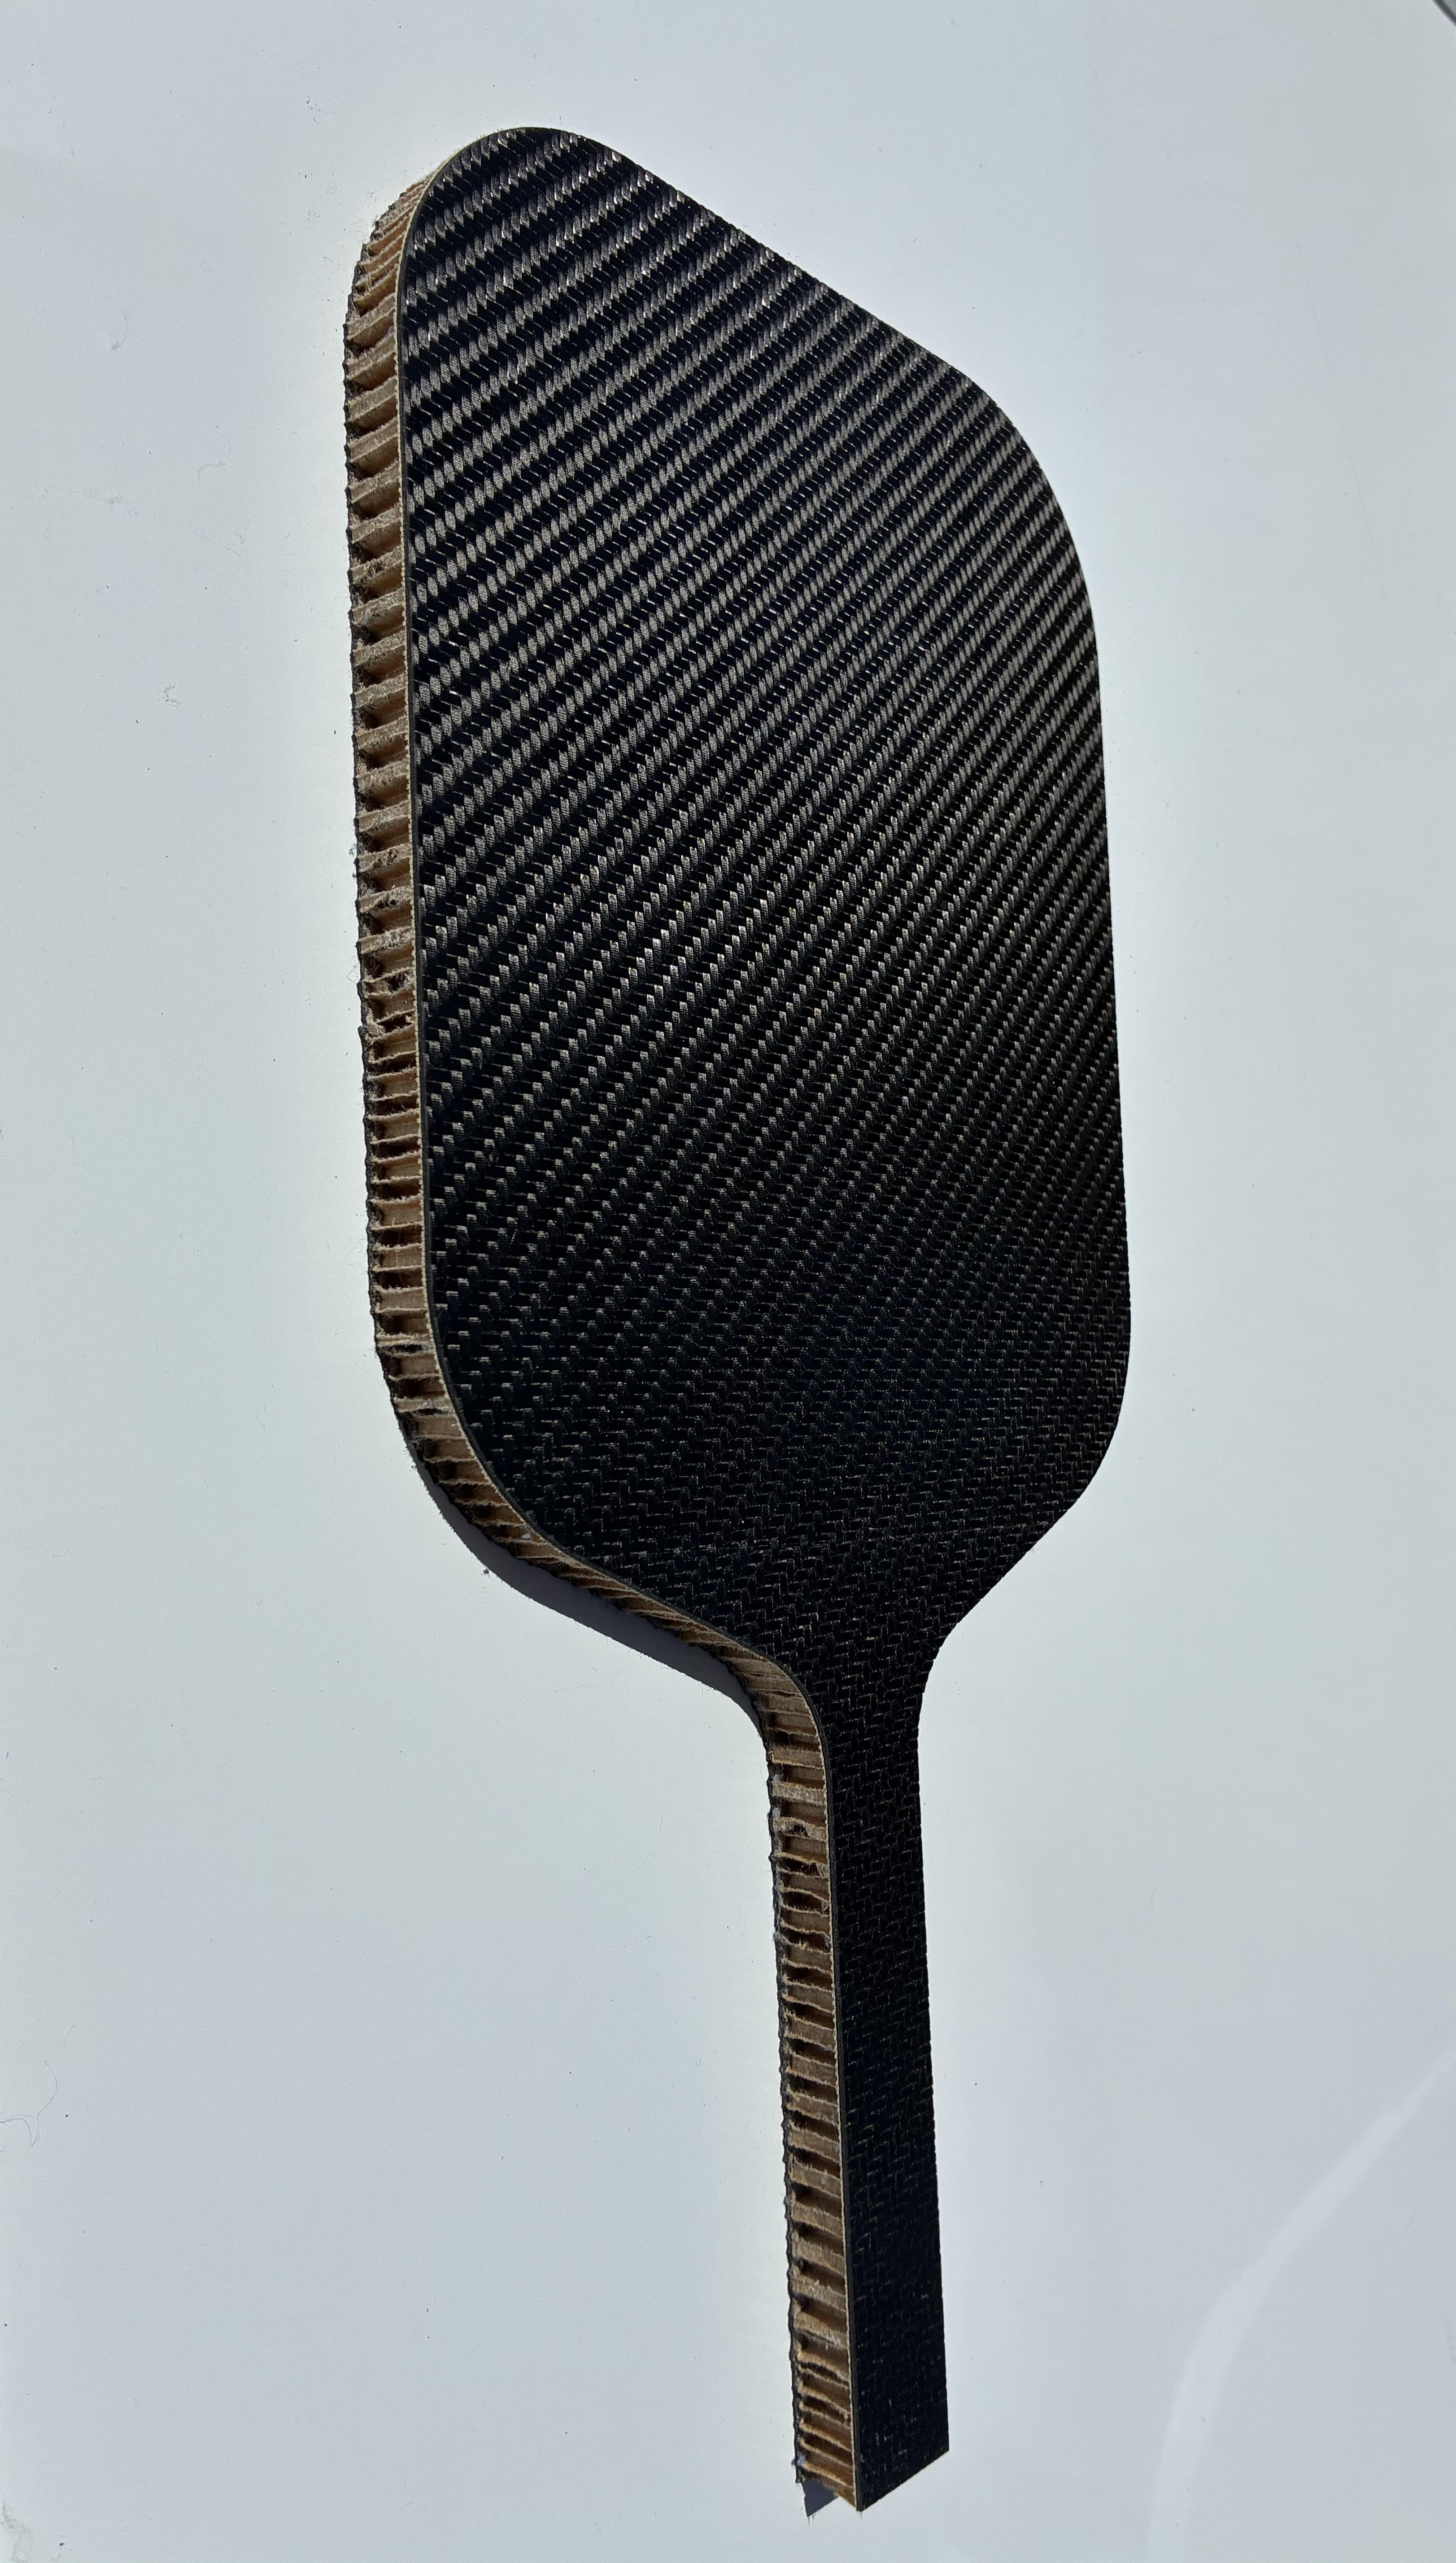
\includegraphics[
        width=1.30in,
        height=1.78in,
        keepaspectratio
    ]{side_core_view}
};

\node[
    anchor=center,
    inner sep=3pt,
    draw=RuleGray,
    line width=0.55pt,
    rounded corners=4pt
]
at ($(current page.north west)+(4.32in,-5.98in)$)
{
    \includegraphics[
        angle=-90,
        origin=c,
        width=1.30in,
        height=1.78in,
        keepaspectratio
    ]{waterjet}
};

\node[
    anchor=north,
    align=center,
    text width=1.38in,
    text=Muted,
    font=\sffamily\fontsize{6.5}{7.1}\selectfont
]
at ($(current page.north west)+(1.12in,-7.00in)$)
{Front view};

\node[
    anchor=north,
    align=center,
    text width=1.38in,
    text=Muted,
    font=\sffamily\fontsize{6.5}{7.1}\selectfont
]
at ($(current page.north west)+(2.72in,-7.00in)$)
{Core and edge profile};

\node[
    anchor=north,
    align=center,
    text width=1.38in,
    text=Muted,
    font=\sffamily\fontsize{6.5}{7.1}\selectfont
]
at ($(current page.north west)+(4.32in,-7.00in)$)
{Waterjet cutting setup};

% ============================================================
% BOTTOM RIGHT — MANUFACTURING HIGHLIGHTS
% ============================================================

\fill[SoftGreen,rounded corners=5pt]
    ($(current page.north west)+(5.18in,-5.05in)$)
    rectangle
    ($(current page.north east)+(-0.42in,-7.18in)$);

\draw[RuleGray,line width=0.55pt,rounded corners=5pt]
    ($(current page.north west)+(5.18in,-5.05in)$)
    rectangle
    ($(current page.north east)+(-0.42in,-7.18in)$);

\node[
    anchor=north west,
    text=DeepGreen,
    font=\sffamily\bfseries\fontsize{7.9}{8.6}\selectfont
]
at ($(current page.north west)+(5.44in,-5.20in)$)
{MANUFACTURING HIGHLIGHTS};

\node[
    anchor=north west,
    align=left,
    text width=5.05in,
    text=Ink,
    font=\fontsize{6.72}{7.82}\selectfont
]
at ($(current page.north west)+(5.44in,-5.49in)$)
{
\textbf{Consolidation.}
Vacuum bagging and distributed weight pressure maintained intimate contact
throughout the prepreg sandwich layup.\\[2.4pt]
\textbf{Surface quality.}
A scarce PTFE release film produced an unusually consistent matte finish
with a subtle sheen and minimal post-processing.\\[2.4pt]
\textbf{Waterjet stability.}
Perimeter weights restrained the cured stock against jet-induced lifting
and rotational moments during cutting.\\[2.4pt]
\textbf{Final assembly.}
A printed TPU edge band protected the carbon perimeter, while the PLA handle
used clearance cutouts to accommodate future stock-thickness and cutting variation.
};

% ============================================================
% RESOURCE LINK
% ============================================================

\node[
    anchor=north,
    align=center,
    text=DeepGreen,
    font=\sffamily\bfseries\fontsize{7.0}{7.6}\selectfont
]
at ($(current page.north)+(0,-7.42in)$)
{\href{\PaddleWaterjetVideo}
{\faPlayCircle\ WATERJET PICKLEBALL PADDLE DEMONSTRATION}};

% ============================================================
% FOOTER
% ============================================================

\node[
    anchor=south west,
    text=white,
    font=\sffamily\bfseries\fontsize{7.1}{7.7}\selectfont
]
at ($(current page.south west)+(0.42in,0.17in)$)
{\hyperlink{toro-results}{\faArrowLeft\ TORO COVER}};

\node[
    anchor=south,
    text=white,
    font=\sffamily\fontsize{7.0}{7.6}\selectfont
]
at ($(current page.south)+(0,0.17in)$)
{PICKLEBALL PADDLE \hspace{6pt} 1 / 1};

\node[
    anchor=south east,
    text=white,
    font=\sffamily\bfseries\fontsize{7.1}{7.7}\selectfont
]
at ($(current page.south east)+(-0.42in,0.17in)$)
{NEXT PROJECT \faArrowRight};

\end{tikzpicture}
%\input{Beam}
%\clearpage

\clearpage


% ============================================================
% TORO COVER — THREE-PAGE PORTFOLIO CASE STUDY
% Pages 3–5 of the complete portfolio
%
% IMPORTANT:
% 1. This file must NOT contain \documentclass, \begin{document},
%    \end{document}, or 
% ============================================================
% TORO COVER — THREE-PAGE PORTFOLIO CASE STUDY
% Pages 3–5 of the complete portfolio
%
% IMPORTANT:
% 1. This file must NOT contain \documentclass, \begin{document},
%    \end{document}, or 
% ============================================================
% TORO COVER — THREE-PAGE PORTFOLIO CASE STUDY
% Pages 3–5 of the complete portfolio
%
% IMPORTANT:
% 1. This file must NOT contain \documentclass, \begin{document},
%    \end{document}, or \input{toro}.
% 2. In main.tex, place \input{toro} before \end{document}.
% 3. Image references use the original Overleaf base filenames
%    without extensions.
% ============================================================



% ============================================================
% CLICKABLE PROJECT RESOURCES
% All links use the exact Google Drive resources supplied.
% ============================================================
\providecommand{\ToroDrawingLink}{https://drive.google.com/file/d/1A7-7wMnRNLuQDaTgxeuUCBsGNqyXzOGV/view?usp=sharing}
\providecommand{\ToroDimensionsLink}{https://drive.google.com/file/d/13sw3BNJvE8GdzlRffxoF2n5r9Gzxide7/view?usp=sharing}
\providecommand{\ToroProblemLink}{https://drive.google.com/file/d/1zHtl8zrb13F1yeN74ptawpfS5UM_xsuw/view?usp=drive_link}
\providecommand{\ToroReportLink}{https://drive.google.com/file/d/1ULZ-P46lFsC2x29ZfmRVIKgYnr9o8hMt/view?usp=drive_link}
\providecommand{\ToroPosterLink}{https://drive.google.com/file/d/1vKiKaJUcHQb_db-FkZnRF6EvtuM4hKyS/view?usp=drive_link}
\providecommand{\ToroDeploymentLink}{https://drive.google.com/file/d/1XJx34o80_mZPTl7xy93HtWAgtS3ThhvY/view?usp=drive_link}
\providecommand{\ToroRemovalLink}{https://drive.google.com/file/d/1O7xYeyB67NUwT-j1B1HeiCcHnZDYjk6_/view?usp=drive_link}

% ============================================================
% PAGE 1 — PROJECT OVERVIEW, OWNERSHIP, AND ARCHITECTURE
% ============================================================

\clearpage
\thispagestyle{empty}
\hypertarget{toro}{}
\null

\begin{tikzpicture}[remember picture,overlay]

% Background
\fill[white]
    (current page.south west)
    rectangle
    (current page.north east);

% Page bars
\fill[DeepGreen]
    (current page.north west)
    rectangle
    ($(current page.north east)+(0,-0.095in)$);

\fill[PolyGold]
    ($(current page.north west)+(0,-0.095in)$)
    rectangle
    ($(current page.north east)+(0,-0.14in)$);

\fill[DeepGreen]
    (current page.south west)
    rectangle
    ($(current page.south east)+(0,0.36in)$);

\fill[PolyGold]
    ($(current page.south west)+(0,0.36in)$)
    rectangle
    ($(current page.south east)+(0,0.405in)$);

% Header
\node[
    anchor=north west,
    text=PolyGold,
    font=\sffamily\bfseries\fontsize{8.1}{8.7}\selectfont
]
at ($(current page.north west)+(0.42in,-0.39in)$)
{01 COMPOSITES \hspace{5pt}/\hspace{5pt} PROJECT 01};

\node[
    anchor=north west,
    text=DeepGreen,
    font=\bfseries\fontsize{23.5}{24.5}\selectfont
]
at ($(current page.north west)+(0.40in,-0.67in)$)
{TORO CARBON FIBER SAFETY COVER};

\node[
    anchor=north west,
    text=Muted,
    font=\sffamily\fontsize{8.4}{9.2}\selectfont
]
at ($(current page.north west)+(0.42in,-1.12in)$)
{Cal Poly Composites Laboratory \hspace{7pt}\textbullet\hspace{7pt}
Team Project \hspace{7pt}\textbullet\hspace{7pt}
Fall--Spring 2026 \hspace{7pt}\textbullet\hspace{7pt}
San Luis Obispo, California};

\fill[PolyGold]
    ($(current page.north west)+(0.42in,-1.37in)$)
    rectangle
    ($(current page.north west)+(6.1in,-1.325in)$);

% Challenge text
\node[
    anchor=north west,
    text=DeepGreen,
    font=\sffamily\bfseries\fontsize{8.1}{8.8}\selectfont
]
at ($(current page.north west)+(0.43in,-1.61in)$)
{THE CHALLENGE};

\node[
    anchor=north west,
    align=left,
    text width=4.47in,
    text=Ink,
    font=\fontsize{8.05}{9.65}\selectfont
]
at ($(current page.north west)+(0.43in,-1.84in)$)
{
Develop a lightweight cover for a 6 ft by 6 ft in-ground spa
that could be deployed by one person, stored compactly,
provide insulation, resist a poolside environment, and maintain
a refined appearance. The sponsor supplied an ambitious but
intentionally broad project statement, requiring the team to
define the product architecture, priorities, manufacturing
strategy, and realistic path toward future commercialization.
};

% Role box
\fill[SoftGold,rounded corners=5pt]
    ($(current page.north west)+(0.42in,-2.88in)$)
    rectangle
    ($(current page.north west)+(4.98in,-4.58in)$);

\fill[PolyGold]
    ($(current page.north west)+(0.42in,-2.88in)$)
    rectangle
    ($(current page.north west)+(0.52in,-4.58in)$);

\node[
    anchor=north west,
    text=DeepGreen,
    font=\sffamily\bfseries\fontsize{8.1}{8.8}\selectfont
]
at ($(current page.north west)+(0.66in,-3.02in)$)
{MY ROLE — DESIGN \& MANUFACTURING LEAD};

\node[
    anchor=north west,
    align=left,
    text width=4.02in,
    text=Ink,
    font=\fontsize{7.05}{8.15}\selectfont
]
at ($(current page.north west)+(0.66in,-3.27in)$)
{
\textbullet\ Modeled every custom part and the complete assembly\\[1.5pt]
\textbullet\ Produced the engineering drawing package independently\\[1.5pt]
\textbullet\ Developed the composite-panel manufacturing process\\[1.5pt]
\textbullet\ Created all waterjet DXFs and manufacturing geometry\\[1.5pt]
\textbullet\ Trained teammates in wet layup and vacuum bagging\\[1.5pt]
\textbullet\ Presented feasibility, scope, and tradeoffs to the sponsor
};

% Large deployed foam-model image
\node[anchor=center,inner sep=0pt]
at ($(current page.north west)+(8.00in,-3.04in)$)
{
    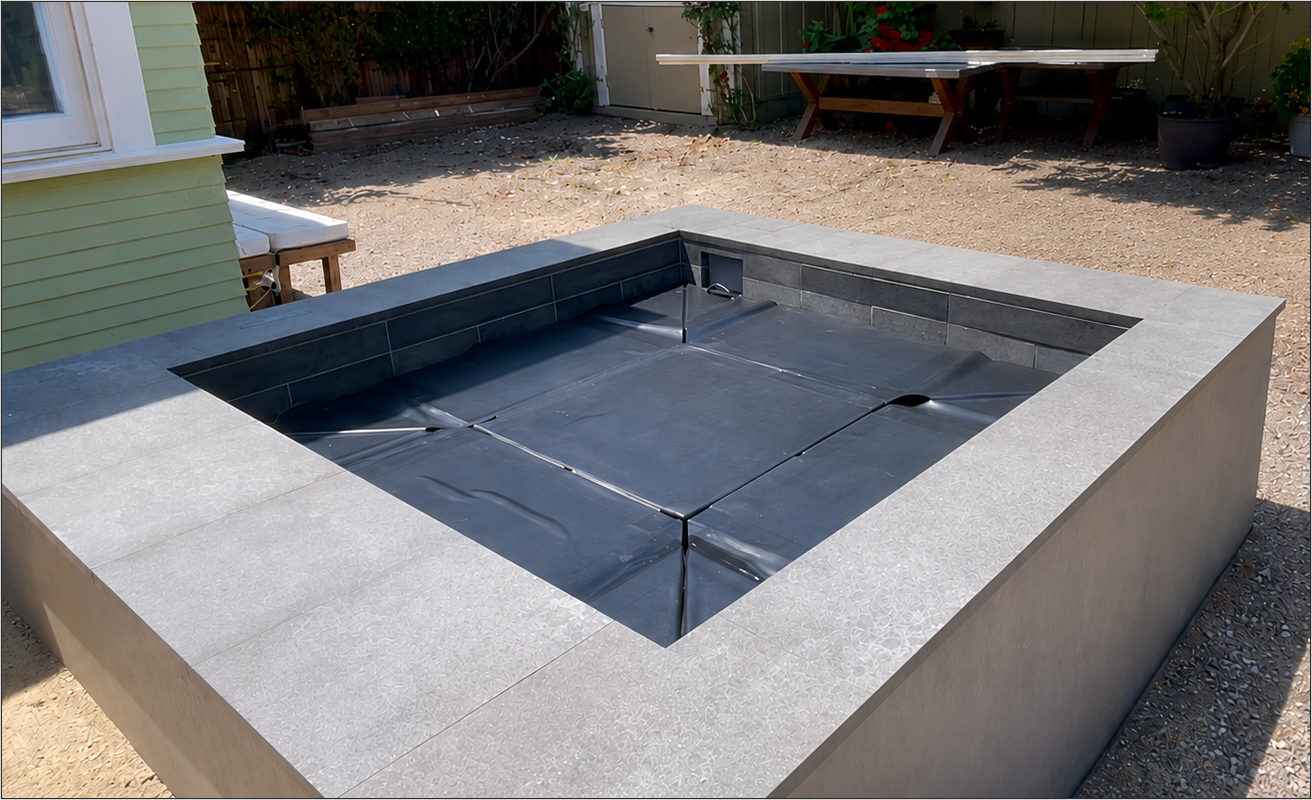
\includegraphics[
        width=5.55in,
        height=2.78in,
        keepaspectratio
    ]{deployed_functional_prototype}
};

\draw[DeepGreen,line width=0.8pt,rounded corners=7pt]
    ($(current page.north west)+(5.16in,-1.61in)$)
    rectangle
    ($(current page.north east)+(-0.42in,-4.47in)$);

\node[
    anchor=north west,
    text=Muted,
    font=\sffamily\fontsize{6.2}{6.9}\selectfont
]
at ($(current page.north west)+(5.18in,-4.54in)$)
{Functional foam model deployed over the sponsor's in-ground spa.};

% Image-strip title
\node[
    anchor=north west,
    text=DeepGreen,
    font=\sffamily\bfseries\fontsize{8.1}{8.8}\selectfont
]
at ($(current page.north west)+(0.43in,-4.78in)$)
{PRODUCT DEVELOPMENT AND FINAL ARCHITECTURE};

% Five-image development strip — CAD-first sequence
% Image 1: topside CAD
\node[anchor=center,inner sep=0pt]
at ($(current page.north west)+(1.47in,-5.73in)$)
{
    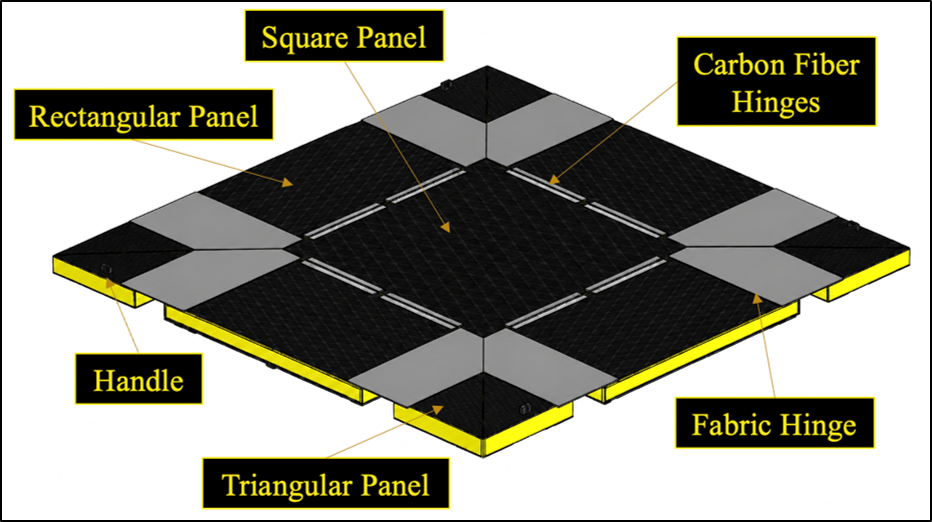
\includegraphics[
        width=1.92in,
        height=1.30in,
        keepaspectratio
    ]{Toro_Cover_topside_Cad}
};
\draw[RuleGray,line width=0.55pt,rounded corners=4pt]
    ($(current page.north west)+(0.43in,-5.04in)$)
    rectangle
    ($(current page.north west)+(2.51in,-6.43in)$);

% Image 2: underside CAD
\node[anchor=center,inner sep=0pt]
at ($(current page.north west)+(3.66in,-5.73in)$)
{
    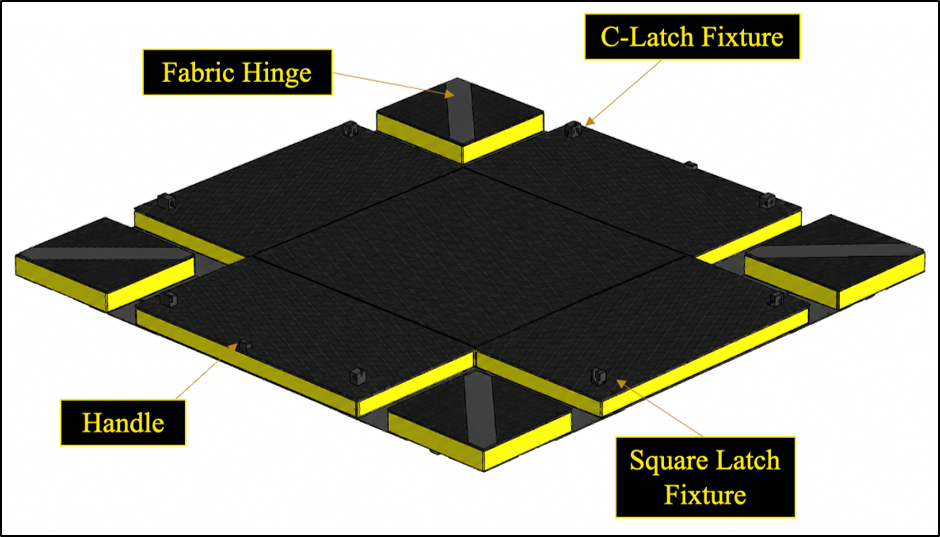
\includegraphics[
        width=1.92in,
        height=1.30in,
        keepaspectratio
    ]{toro_cover_underside_cad}
};
\draw[RuleGray,line width=0.55pt,rounded corners=4pt]
    ($(current page.north west)+(2.62in,-5.04in)$)
    rectangle
    ($(current page.north west)+(4.70in,-6.43in)$);

% Image 3: folded CAD
\node[anchor=center,inner sep=0pt]
at ($(current page.north west)+(5.85in,-5.73in)$)
{
    \includegraphics[
        width=1.92in,
        height=1.30in,
        keepaspectratio
    ]{\detokenize{Toro_Cover_folded Configuration}}
};
\draw[RuleGray,line width=0.55pt,rounded corners=4pt]
    ($(current page.north west)+(4.81in,-5.04in)$)
    rectangle
    ($(current page.north west)+(6.89in,-6.43in)$);

% Image 4: dual-use product concept
\node[anchor=center,inner sep=0pt]
at ($(current page.north west)+(8.04in,-5.73in)$)
{
    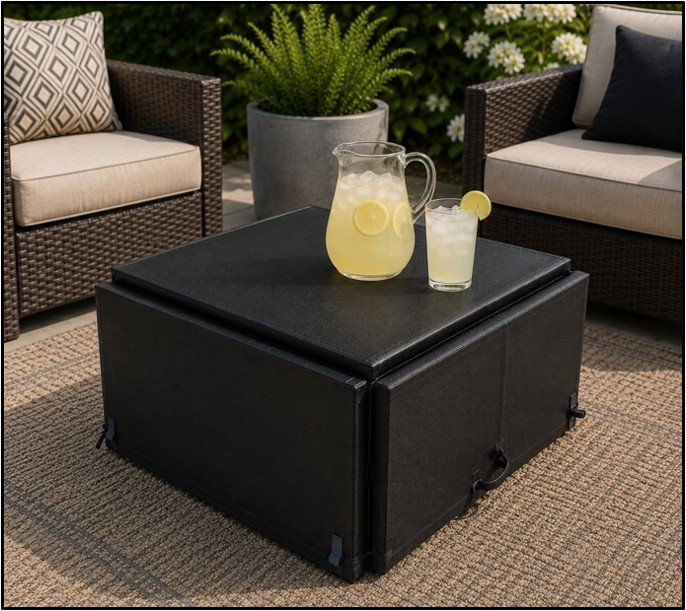
\includegraphics[
        width=1.92in,
        height=1.30in,
        keepaspectratio
    ]{generative_AI_concept_toro_cover_art}
};
\draw[RuleGray,line width=0.55pt,rounded corners=4pt]
    ($(current page.north west)+(7.00in,-5.04in)$)
    rectangle
    ($(current page.north west)+(9.08in,-6.43in)$);

% Image 5: folded foam functional prototype
% The portrait photograph is deliberately clipped to the landscape frame
% so the ottoman fills the card without extending beyond its border.
\begin{scope}
\clip[rounded corners=4pt]
    ($(current page.north west)+(9.19in,-5.04in)$)
    rectangle
    ($(current page.north east)+(-0.43in,-6.43in)$);

% Keep the original image proportions and center it within the existing card.
\node[anchor=center,inner sep=0pt]
at ($(current page.north west)+(9.88in,-5.735in)$)
{
    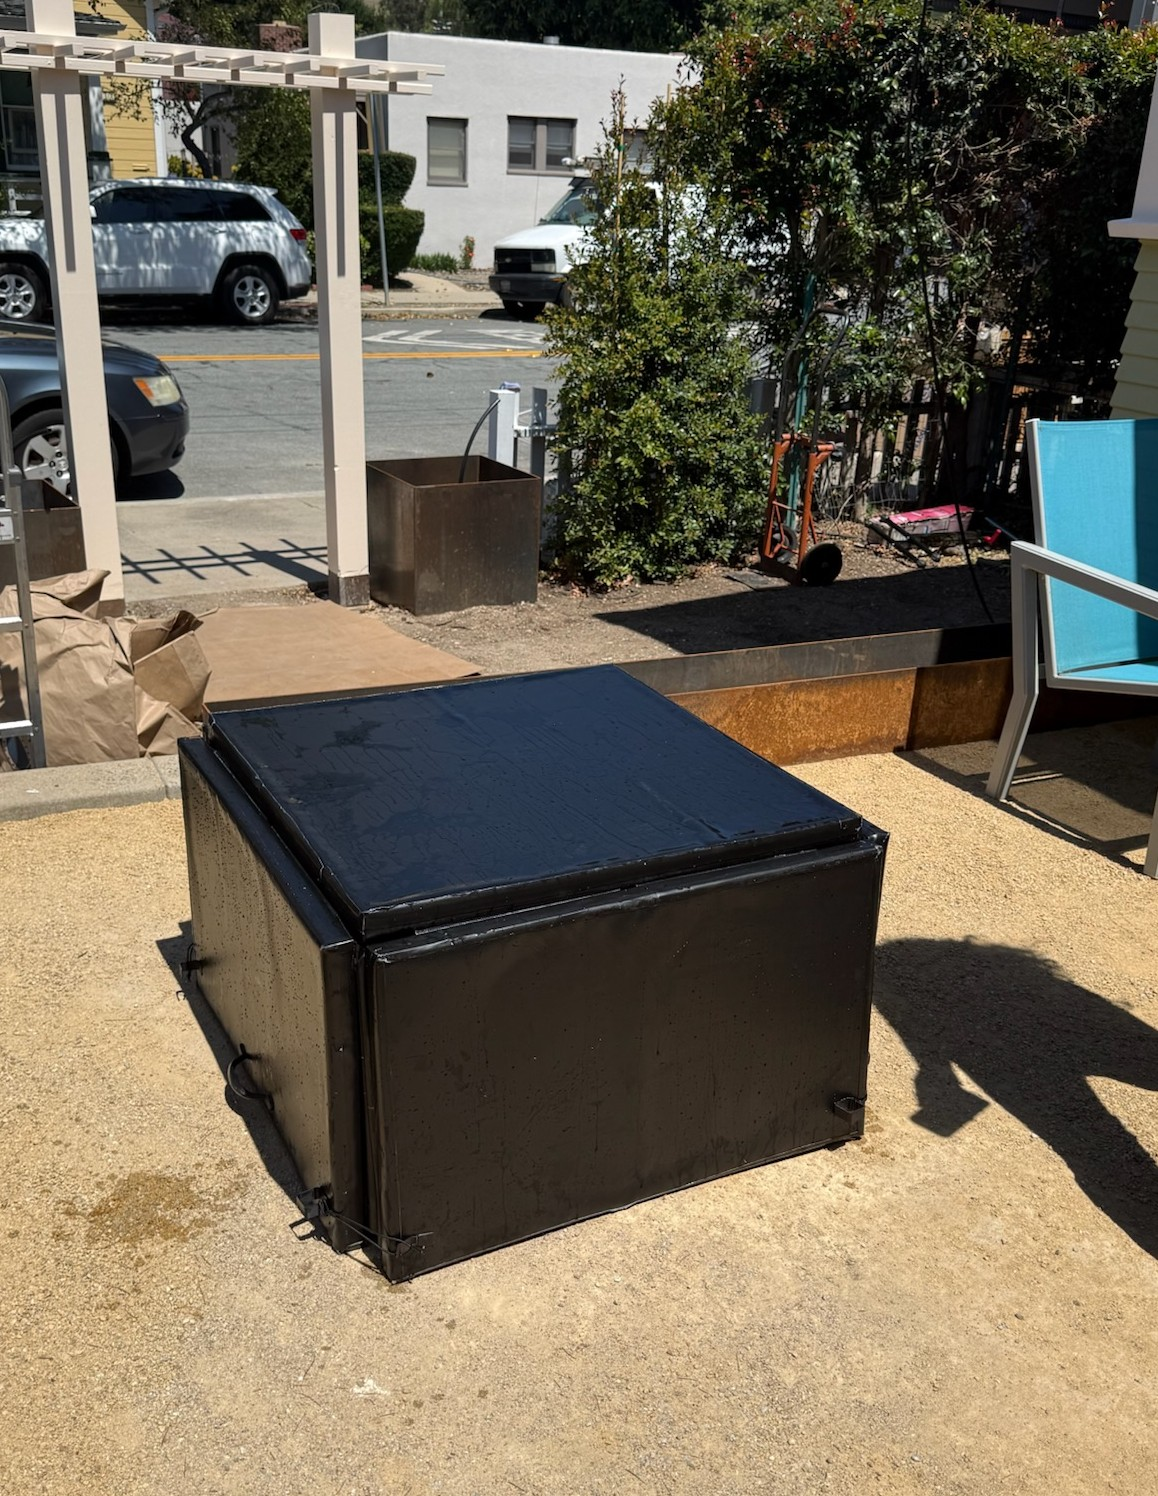
\includegraphics[
        width=1.58in,
        height=1.28in,
        keepaspectratio
    ]{foam_model_folded_backyard_image}
};
\end{scope}

\draw[RuleGray,line width=0.55pt,rounded corners=4pt]
    ($(current page.north west)+(9.19in,-5.04in)$)
    rectangle
    ($(current page.north east)+(-0.43in,-6.43in)$);

% Larger captions
\node[anchor=north,align=center,text width=1.95in,text=Muted,
      font=\sffamily\fontsize{6.8}{7.4}\selectfont]
at ($(current page.north west)+(1.47in,-6.49in)$)
{Topside panel architecture};

\node[anchor=north,align=center,text width=1.95in,text=Muted,
      font=\sffamily\fontsize{6.8}{7.4}\selectfont]
at ($(current page.north west)+(3.66in,-6.49in)$)
{Underside hinge architecture};

\node[anchor=north,align=center,text width=1.95in,text=Muted,
      font=\sffamily\fontsize{6.8}{7.4}\selectfont]
at ($(current page.north west)+(5.85in,-6.49in)$)
{Folded CAD configuration};

\node[anchor=north,align=center,text width=1.95in,text=Muted,
      font=\sffamily\fontsize{6.8}{7.4}\selectfont]
at ($(current page.north west)+(8.04in,-6.49in)$)
{Dual-use product vision};

\node[anchor=north,align=center,text width=1.95in,text=Muted,
      font=\sffamily\fontsize{6.8}{7.4}\selectfont]
at ($(current page.north west)+(9.88in,-6.49in)$)
{Folded foam prototype};

% Page 1 resource bar — centered and non-repeated resources
\fill[Panel,rounded corners=4pt]
    ($(current page.north west)+(0.43in,-7.05in)$)
    rectangle
    ($(current page.north east)+(-0.43in,-7.64in)$);
\draw[RuleGray,line width=0.5pt,rounded corners=4pt]
    ($(current page.north west)+(0.43in,-7.05in)$)
    rectangle
    ($(current page.north east)+(-0.43in,-7.64in)$);

\node[
    anchor=center,
    align=center,
    text=DeepGreen,
    font=\sffamily\bfseries\fontsize{6.9}{7.5}\selectfont
]
at ($(current page.north)+(0,-7.345in)$)
{\href{\ToroDrawingLink}{\faDraftingCompass\ DRAWING PACKAGE}
\hspace{24pt}
\href{\ToroDimensionsLink}{\faImage\ DIMENSION STUDY}
\hspace{24pt}
\href{\ToroProblemLink}{\faFileImage\ PROBLEM STATEMENT}};

% Footer
\node[
    anchor=south west,
    text=white,
    font=\sffamily\bfseries\fontsize{7.1}{7.7}\selectfont
]
at ($(current page.south west)+(0.42in,0.17in)$)
{\hyperlink{composites}{\faArrowLeft\ COMPOSITES}};

\node[
    anchor=south,
    text=white,
    font=\sffamily\fontsize{7.0}{7.6}\selectfont
]
at ($(current page.south)+(0,0.17in)$)
{TORO COVER \hspace{6pt} 1 / 3};

\node[
    anchor=south east,
    text=white,
    font=\sffamily\bfseries\fontsize{7.1}{7.7}\selectfont
]
at ($(current page.south east)+(-0.42in,0.17in)$)
{MANUFACTURING-DRIVEN DESIGN \faArrowRight};

\end{tikzpicture}


% ============================================================
% PAGE 2 — MANUFACTURING-DRIVEN DESIGN
% ============================================================

\clearpage
\thispagestyle{empty}
\hypertarget{toro-manufacturing}{}
\null

\begin{tikzpicture}[remember picture,overlay]

% Background and bars
\fill[white]
    (current page.south west)
    rectangle
    (current page.north east);

\fill[DeepGreen]
    (current page.north west)
    rectangle
    ($(current page.north east)+(0,-0.095in)$);

\fill[PolyGold]
    ($(current page.north west)+(0,-0.095in)$)
    rectangle
    ($(current page.north east)+(0,-0.14in)$);

\fill[DeepGreen]
    (current page.south west)
    rectangle
    ($(current page.south east)+(0,0.36in)$);

\fill[PolyGold]
    ($(current page.south west)+(0,0.36in)$)
    rectangle
    ($(current page.south east)+(0,0.405in)$);

% Header
\node[
    anchor=north west,
    text=PolyGold,
    font=\sffamily\bfseries\fontsize{8.1}{8.7}\selectfont
]
at ($(current page.north west)+(0.42in,-0.39in)$)
{TORO COVER \hspace{5pt}/\hspace{5pt} DESIGN FOR MANUFACTURABILITY};

\node[
    anchor=north west,
    text=DeepGreen,
    font=\bfseries\fontsize{23}{24}\selectfont
]
at ($(current page.north west)+(0.40in,-0.67in)$)
{THE ENVELOPE METHOD};

\node[
    anchor=north west,
    text=Muted,
    font=\sffamily\fontsize{8.7}{9.6}\selectfont
]
at ($(current page.north west)+(0.42in,-1.12in)$)
{A one-layup process developed for unusually thick insulated composite sandwich panels};

\fill[PolyGold]
    ($(current page.north west)+(0.42in,-1.36in)$)
    rectangle
    ($(current page.north west)+(5.30in,-1.315in)$);

% Process explanation
\fill[SoftGold,rounded corners=5pt]
    ($(current page.north west)+(0.42in,-1.61in)$)
    rectangle
    ($(current page.north east)+(-0.42in,-2.90in)$);

\fill[PolyGold]
    ($(current page.north west)+(0.42in,-1.61in)$)
    rectangle
    ($(current page.north west)+(0.52in,-2.90in)$);

\node[
    anchor=north west,
    text=DeepGreen,
    font=\sffamily\bfseries\fontsize{7.9}{8.6}\selectfont
]
at ($(current page.north west)+(0.67in,-1.76in)$)
{PROCESS INNOVATION};

\node[
    anchor=north west,
    align=left,
    text width=9.55in,
    text=Ink,
    font=\fontsize{7.35}{8.75}\selectfont
]
at ($(current page.north west)+(0.67in,-2.02in)$)
{
Weight reduction and insulation were both essential, leading to the selection of an
XPS foam core. Because XPS could not tolerate composite heat-cure temperatures, prepreg
processing was not practical and the panels had to be manufactured by wet layup with a
room-temperature cure. To simplify this process, I waterjet-cut XPS perimeter strips from
excess foam and placed them around each core inside the vacuum enclosure. Under vacuum,
the top and bottom carbon skins met along the panel sides and compressed against this
border, eliminating a separate edge-banding layup and reducing corner pleating.
};

% Workflow title
\node[
    anchor=north west,
    text=DeepGreen,
    font=\sffamily\bfseries\fontsize{8.0}{8.7}\selectfont
]
at ($(current page.north west)+(0.43in,-3.06in)$)
{MANUFACTURING WORKFLOW};

% Row 1 image 1
\node[anchor=center,inner sep=0pt]
at ($(current page.north west)+(2.07in,-4.105in)$)
{
    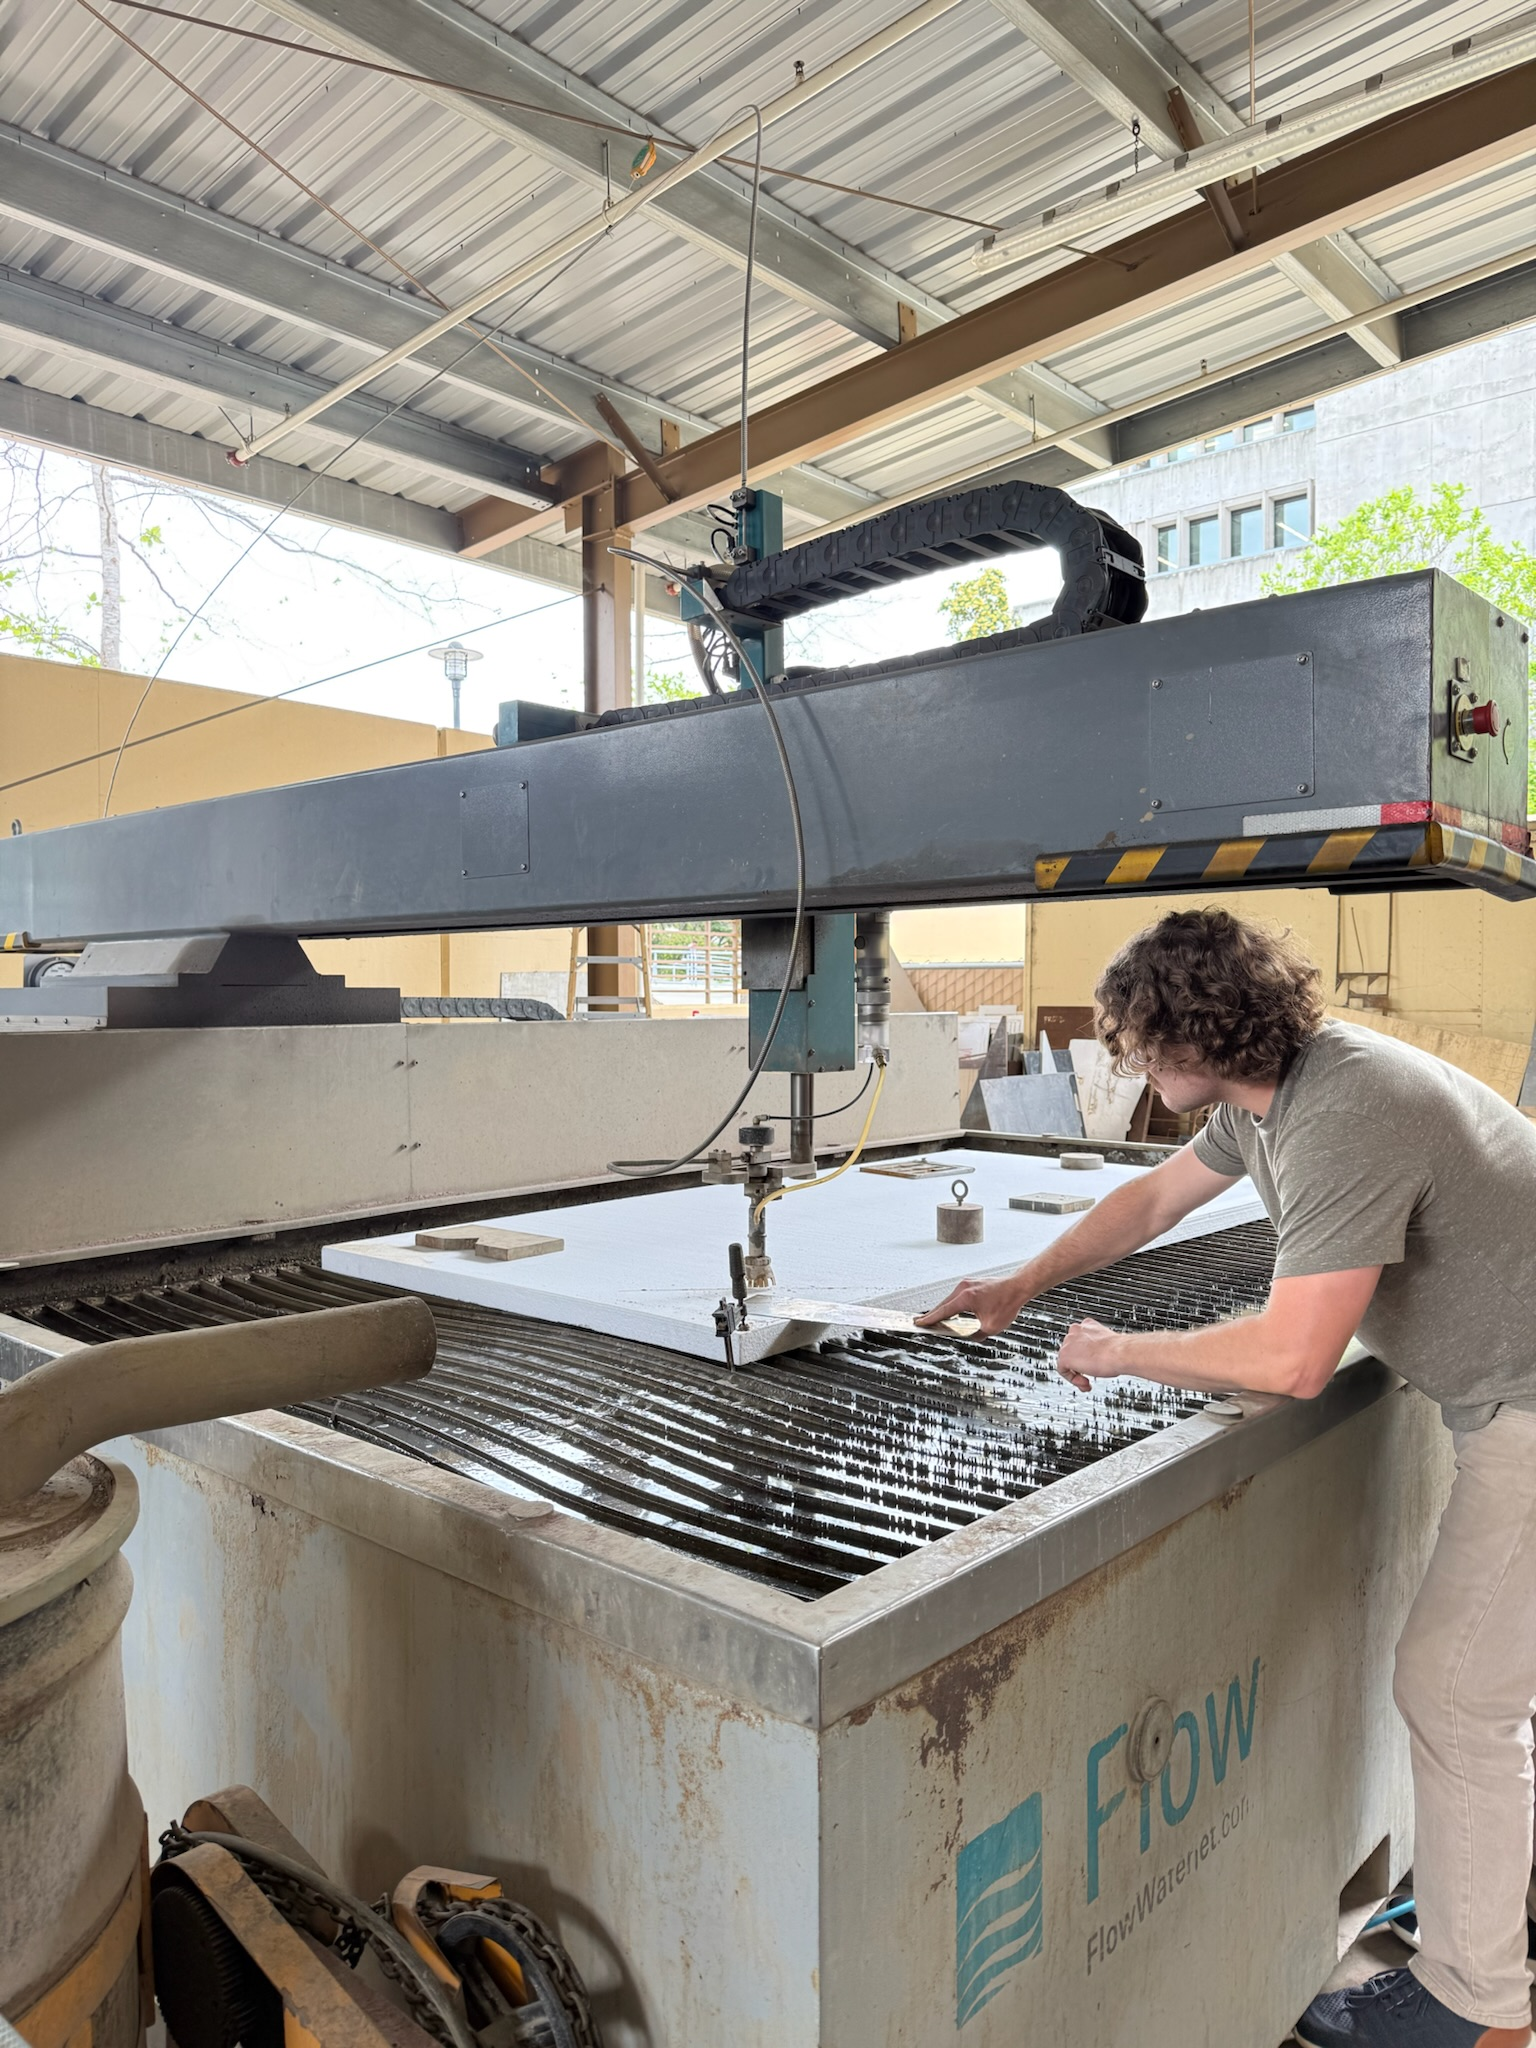
\includegraphics[
        width=3.10in,
        height=1.40in,
        keepaspectratio
    ]{waterjet_foam}
};
\draw[RuleGray,line width=0.55pt,rounded corners=4pt]
    ($(current page.north west)+(0.43in,-3.36in)$)
    rectangle
    ($(current page.north west)+(3.71in,-4.85in)$);

% Row 1 image 2
\node[anchor=center,inner sep=0pt]
at ($(current page.north west)+(5.50in,-4.105in)$)
{
    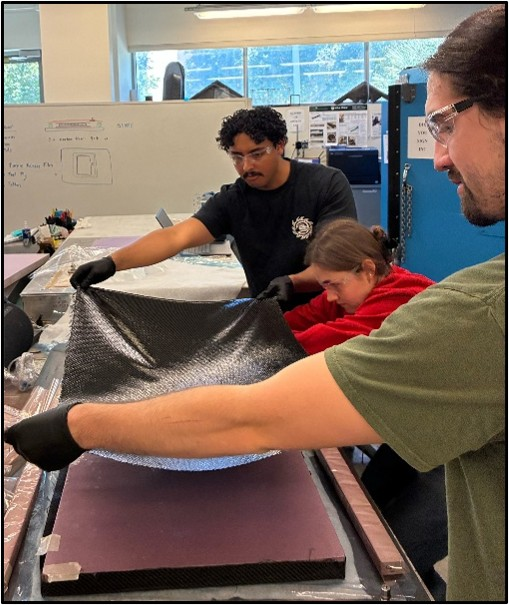
\includegraphics[
        width=3.10in,
        height=1.40in,
        keepaspectratio
    ]{group_layup}
};
\draw[RuleGray,line width=0.55pt,rounded corners=4pt]
    ($(current page.north west)+(3.86in,-3.36in)$)
    rectangle
    ($(current page.north west)+(7.14in,-4.85in)$);

% Row 1 image 3
\node[anchor=center,inner sep=0pt]
at ($(current page.north west)+(8.935in,-4.105in)$)
{
    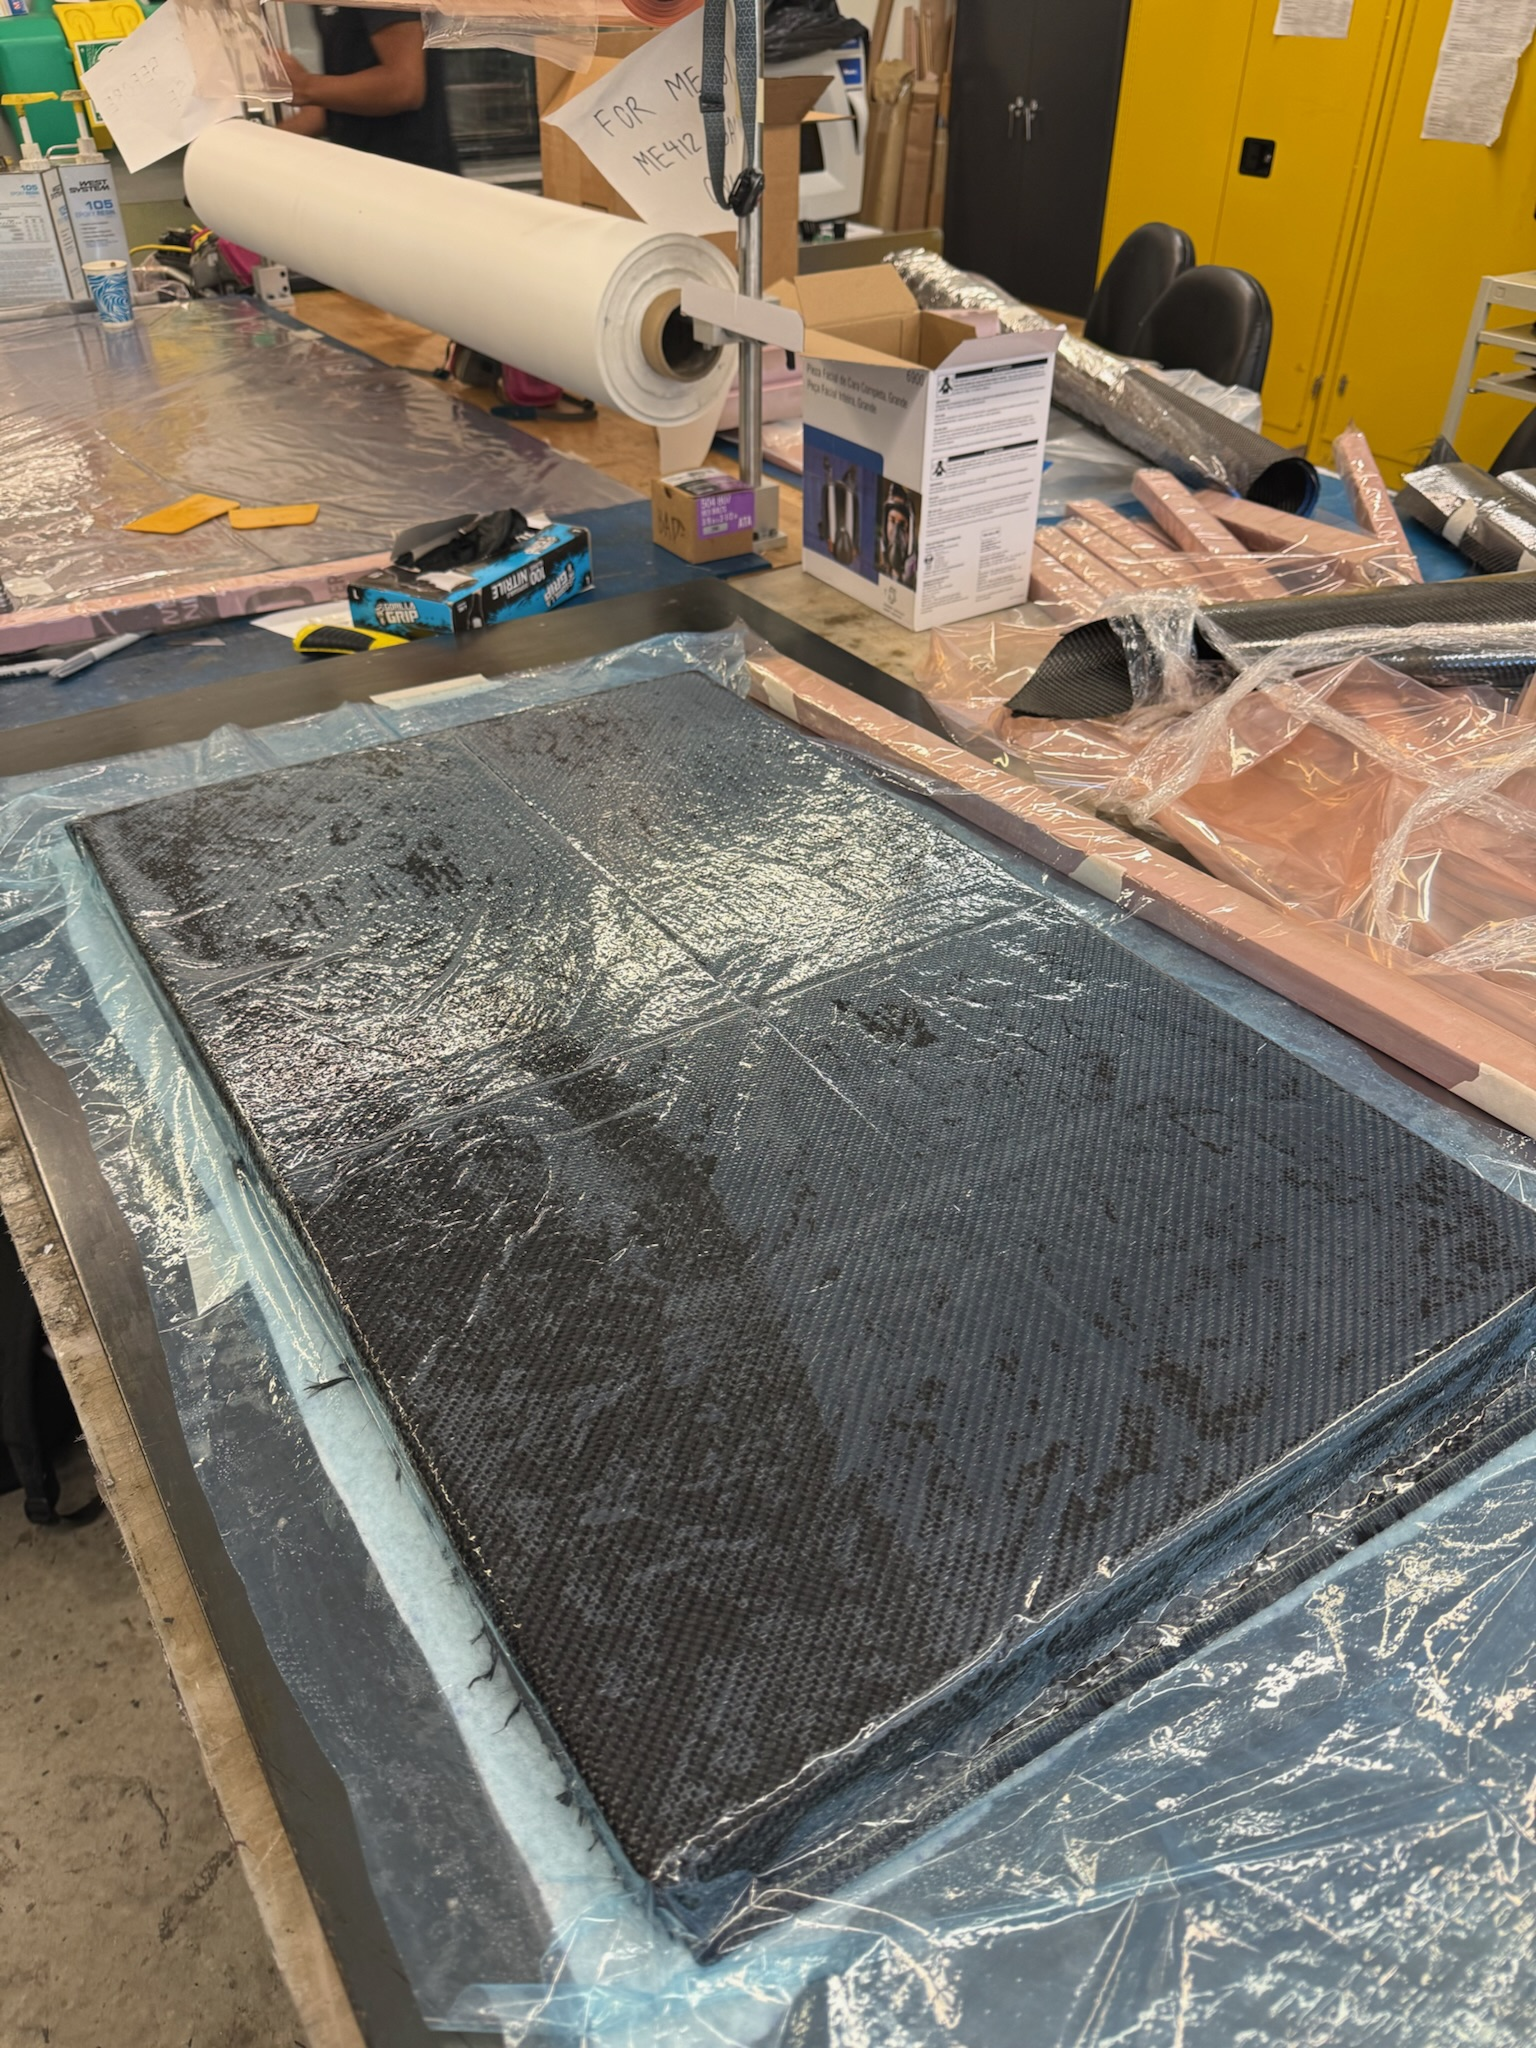
\includegraphics[
        width=3.10in,
        height=1.40in,
        keepaspectratio
    ]{blue_perforrated_film_layup}
};
\draw[RuleGray,line width=0.55pt,rounded corners=4pt]
    ($(current page.north west)+(7.29in,-3.36in)$)
    rectangle
    ($(current page.north east)+(-0.42in,-4.85in)$);

% Row 1 captions
\node[anchor=north,text=Muted,font=\sffamily\fontsize{6.7}{7.3}\selectfont]
at ($(current page.north west)+(2.07in,-4.90in)$)
{1. Waterjet-cut core and perimeter geometry};

\node[anchor=north,text=Muted,font=\sffamily\fontsize{6.7}{7.3}\selectfont]
at ($(current page.north west)+(5.50in,-4.90in)$)
{2. Team wet layup under my process guidance};

\node[anchor=north,text=Muted,font=\sffamily\fontsize{6.7}{7.3}\selectfont]
at ($(current page.north west)+(8.935in,-4.90in)$)
{3. Perforated film, breather, and vacuum enclosure};

% Row 2 image 1
\node[anchor=center,inner sep=0pt]
at ($(current page.north west)+(2.07in,-5.875in)$)
{
    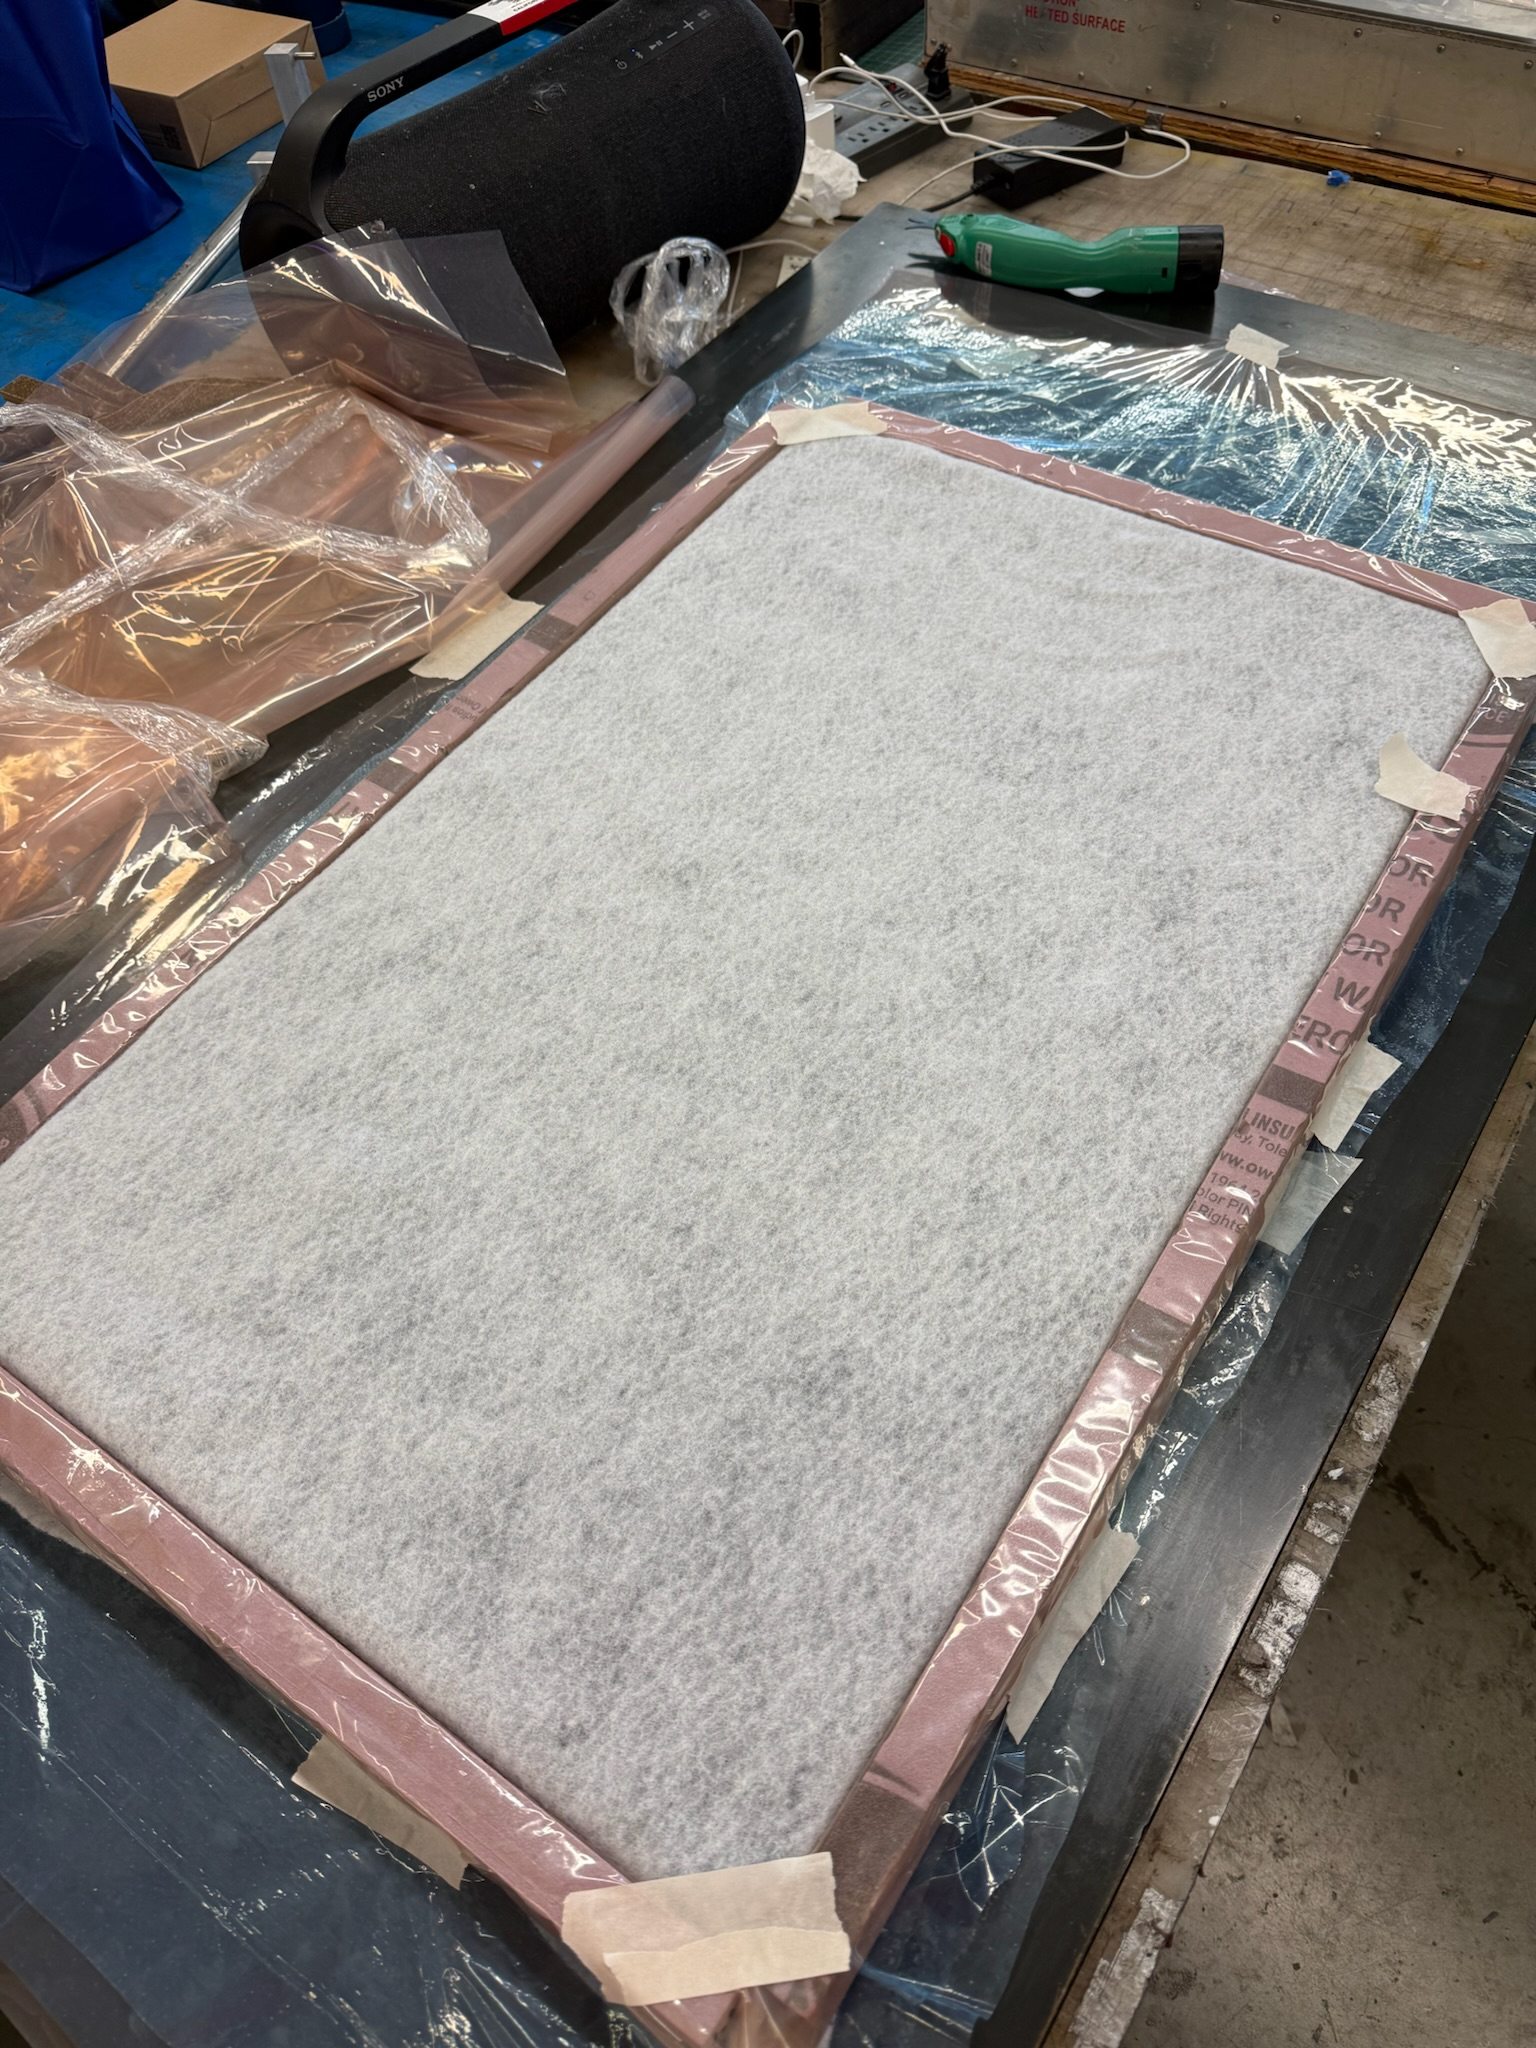
\includegraphics[
        width=3.10in,
        height=1.40in,
        keepaspectratio
    ]{completed_layup}
};
\draw[RuleGray,line width=0.55pt,rounded corners=4pt]
    ($(current page.north west)+(0.43in,-5.13in)$)
    rectangle
    ($(current page.north west)+(3.71in,-6.62in)$);

% Row 2 image 2 — oven chamber used only as a reliable vacuum enclosure; no heat applied
\node[anchor=center,inner sep=0pt]
at ($(current page.north west)+(5.50in,-5.875in)$)
{
    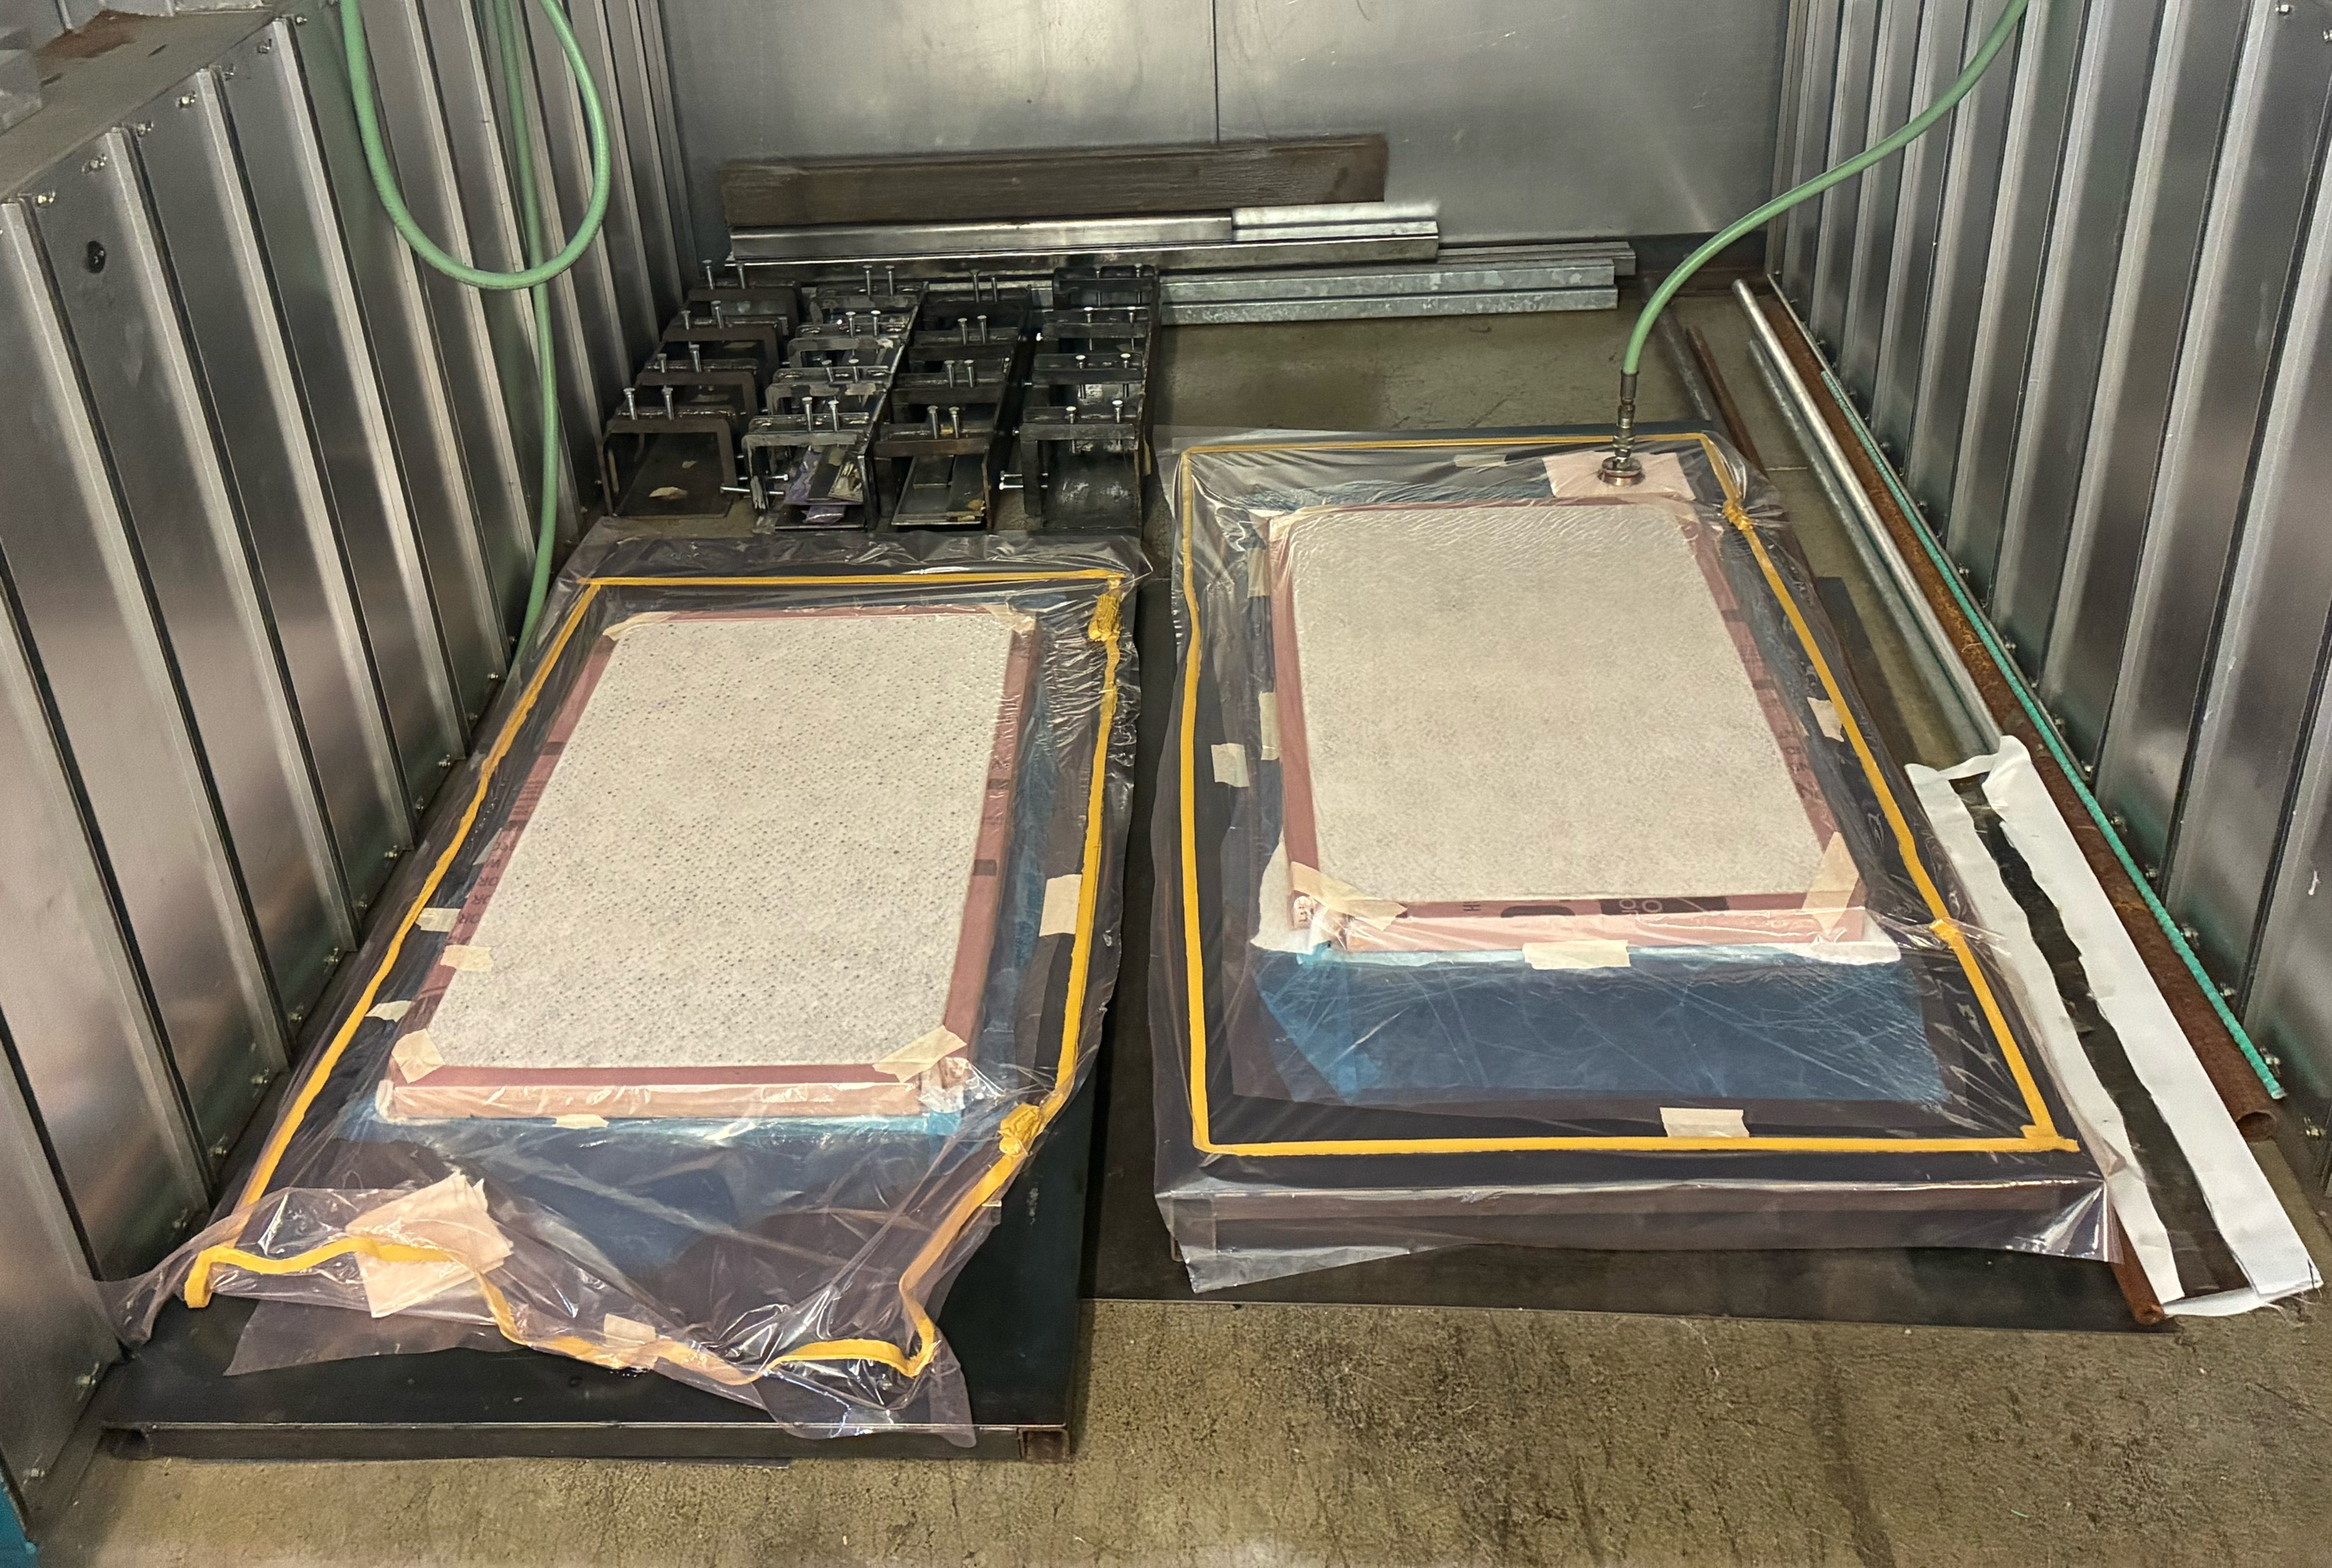
\includegraphics[
        width=3.10in,
        height=1.40in,
        keepaspectratio
    ]{layups_in_composite_oven_under_vacuumPressure}
};
\draw[RuleGray,line width=0.55pt,rounded corners=4pt]
    ($(current page.north west)+(3.86in,-5.13in)$)
    rectangle
    ($(current page.north west)+(7.14in,-6.62in)$);

% Row 2 image 3
\node[anchor=center,inner sep=0pt]
at ($(current page.north west)+(8.935in,-5.875in)$)
{
    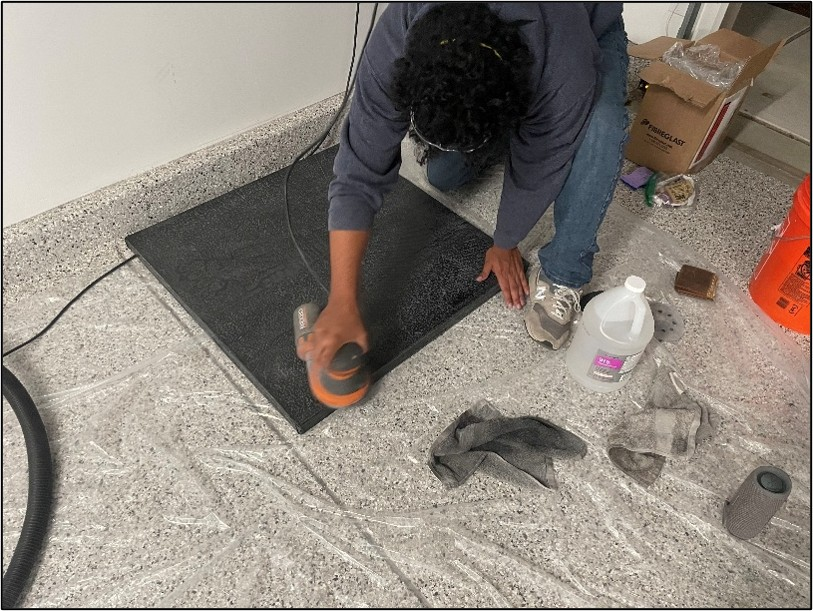
\includegraphics[
        width=3.10in,
        height=1.40in,
        keepaspectratio
    ]{garage_sanding}
};
\draw[RuleGray,line width=0.55pt,rounded corners=4pt]
    ($(current page.north west)+(7.29in,-5.13in)$)
    rectangle
    ($(current page.north east)+(-0.42in,-6.62in)$);

% Row 2 captions
\node[anchor=north,text=Muted,font=\sffamily\fontsize{6.7}{7.3}\selectfont]
at ($(current page.north west)+(2.07in,-6.67in)$)
{4. Fully saturated carbon skin and foam sandwich};

\node[anchor=north,text=Muted,font=\sffamily\fontsize{6.7}{7.3}\selectfont]
at ($(current page.north west)+(5.50in,-6.67in)$)
{5. Room-temperature cure under continuous vacuum};

\node[anchor=north,text=Muted,font=\sffamily\fontsize{6.7}{7.3}\selectfont]
at ($(current page.north west)+(8.935in,-6.67in)$)
{6. Post-processing and surface preparation};

% Bottom callouts
\fill[Panel,rounded corners=4pt]
    ($(current page.north west)+(0.43in,-6.95in)$)
    rectangle
    ($(current page.north west)+(5.48in,-7.60in)$);

\draw[RuleGray,line width=0.55pt,rounded corners=4pt]
    ($(current page.north west)+(0.43in,-6.95in)$)
    rectangle
    ($(current page.north west)+(5.48in,-7.60in)$);

\node[
    anchor=north west,
    text=DeepGreen,
    font=\sffamily\bfseries\fontsize{7.0}{7.6}\selectfont
]
at ($(current page.north west)+(0.63in,-7.08in)$)
{FROM THREE LAYUPS TO ONE};

\node[
    anchor=north west,
    align=left,
    text width=4.56in,
    text=Ink,
    font=\fontsize{6.45}{7.45}\selectfont
]
at ($(current page.north west)+(0.63in,-7.29in)$)
{
The Envelope Method reduced labor, cure cycles, handling,
alignment risk, and time spent forming numerous vacuum-bag
pleats around the 1.5-inch-thick XPS panels.
};

\fill[Panel,rounded corners=4pt]
    ($(current page.north west)+(5.68in,-6.95in)$)
    rectangle
    ($(current page.north east)+(-0.42in,-7.60in)$);

\draw[RuleGray,line width=0.55pt,rounded corners=4pt]
    ($(current page.north west)+(5.68in,-6.95in)$)
    rectangle
    ($(current page.north east)+(-0.42in,-7.60in)$);

\node[
    anchor=north west,
    text=DeepGreen,
    font=\sffamily\bfseries\fontsize{7.0}{7.6}\selectfont
]
at ($(current page.north west)+(5.88in,-7.08in)$)
{WHY SURFACE-BONDED HARDWARE};

\node[
    anchor=north west,
    align=left,
    text width=4.55in,
    text=Ink,
    font=\fontsize{6.45}{7.45}\selectfont
]
at ($(current page.north west)+(5.88in,-7.29in)$)
{
Adhesively bonded hinges and fixtures preserved the clean
composite exterior and avoided drilled inserts, foam-core
crushing, added stress concentrations, and new leak paths.
};


% Footer
\node[
    anchor=south west,
    text=white,
    font=\sffamily\bfseries\fontsize{7.1}{7.7}\selectfont
]
at ($(current page.south west)+(0.42in,0.17in)$)
{\faArrowLeft\ PRODUCT ARCHITECTURE};

\node[
    anchor=south,
    text=white,
    font=\sffamily\fontsize{7.0}{7.6}\selectfont
]
at ($(current page.south)+(0,0.17in)$)
{TORO COVER \hspace{6pt} 2 / 3};

\node[
    anchor=south east,
    text=white,
    font=\sffamily\bfseries\fontsize{7.1}{7.7}\selectfont
]
at ($(current page.south east)+(-0.42in,0.17in)$)
{VALIDATION \& TAKEAWAYS \faArrowRight};

\end{tikzpicture}


% ============================================================
% PAGE 3 — FINISHING, VALIDATION, AND TAKEAWAYS
% ============================================================

\clearpage
\thispagestyle{empty}
\hypertarget{toro-results}{}
\null

\begin{tikzpicture}[remember picture,overlay]

% Background and bars
\fill[white]
    (current page.south west)
    rectangle
    (current page.north east);

\fill[DeepGreen]
    (current page.north west)
    rectangle
    ($(current page.north east)+(0,-0.095in)$);

\fill[PolyGold]
    ($(current page.north west)+(0,-0.095in)$)
    rectangle
    ($(current page.north east)+(0,-0.14in)$);

\fill[DeepGreen]
    (current page.south west)
    rectangle
    ($(current page.south east)+(0,0.36in)$);

\fill[PolyGold]
    ($(current page.south west)+(0,0.36in)$)
    rectangle
    ($(current page.south east)+(0,0.405in)$);

% Header
\node[
    anchor=north west,
    text=PolyGold,
    font=\sffamily\bfseries\fontsize{8.1}{8.7}\selectfont
]
at ($(current page.north west)+(0.42in,-0.39in)$)
{TORO COVER \hspace{5pt}/\hspace{5pt} VALIDATION AND ENGINEERING TAKEAWAYS};

\node[
    anchor=north west,
    text=DeepGreen,
    font=\bfseries\fontsize{22.5}{23.5}\selectfont
]
at ($(current page.north west)+(0.40in,-0.67in)$)
{FROM PROTOTYPE TO PRODUCT PATHWAY};

\node[
    anchor=north west,
    text=Muted,
    font=\sffamily\fontsize{8.7}{9.6}\selectfont
]
at ($(current page.north west)+(0.42in,-1.12in)$)
{Environmental protection, usability testing, scope decisions, and lessons from technical leadership};

\fill[PolyGold]
    ($(current page.north west)+(0.42in,-1.36in)$)
    rectangle
    ($(current page.north west)+(5.8in,-1.315in)$);

% Finishing title
\node[
    anchor=north west,
    text=DeepGreen,
    font=\sffamily\bfseries\fontsize{8.0}{8.7}\selectfont
]
at ($(current page.north west)+(0.43in,-1.62in)$)
{OUTDOOR FINISHING AND ENVIRONMENTAL PROTECTION};

% Image 1
\node[anchor=center,inner sep=0pt]
at ($(current page.north west)+(1.705in,-2.655in)$)
{
    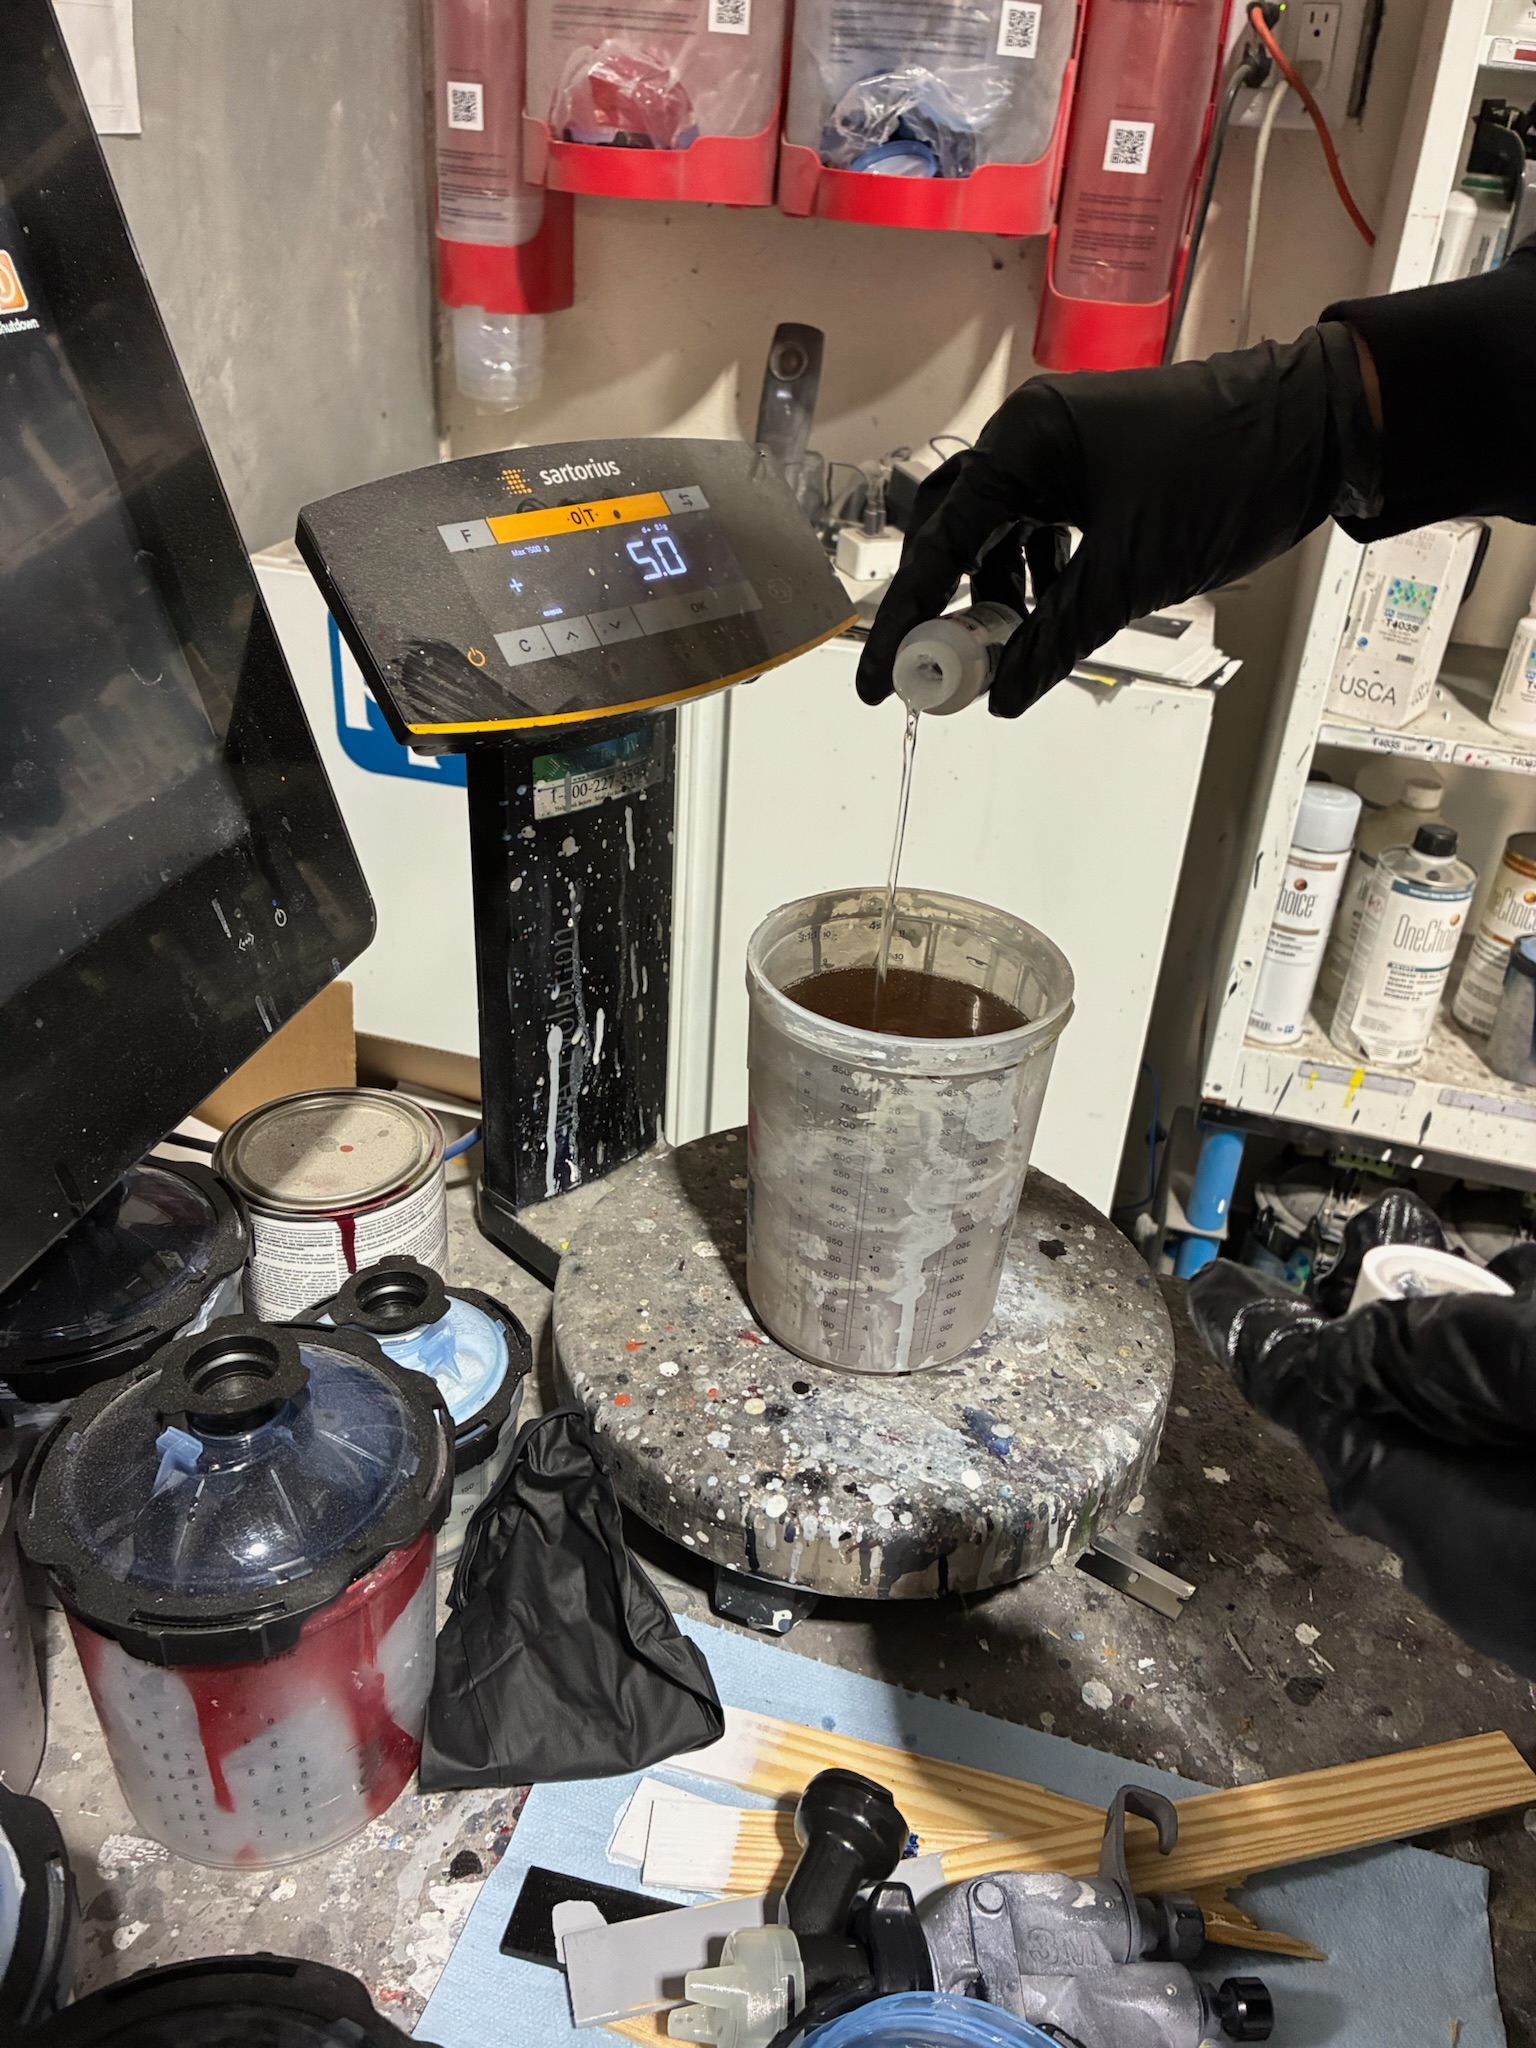
\includegraphics[
        width=2.35in,
        height=1.40in,
        keepaspectratio
    ]{spray_topcoat_prep}
};
\draw[RuleGray,line width=0.55pt,rounded corners=4pt]
    ($(current page.north west)+(0.43in,-1.91in)$)
    rectangle
    ($(current page.north west)+(2.98in,-3.40in)$);

% Image 2
\node[anchor=center,inner sep=0pt]
at ($(current page.north west)+(4.375in,-2.655in)$)
{
    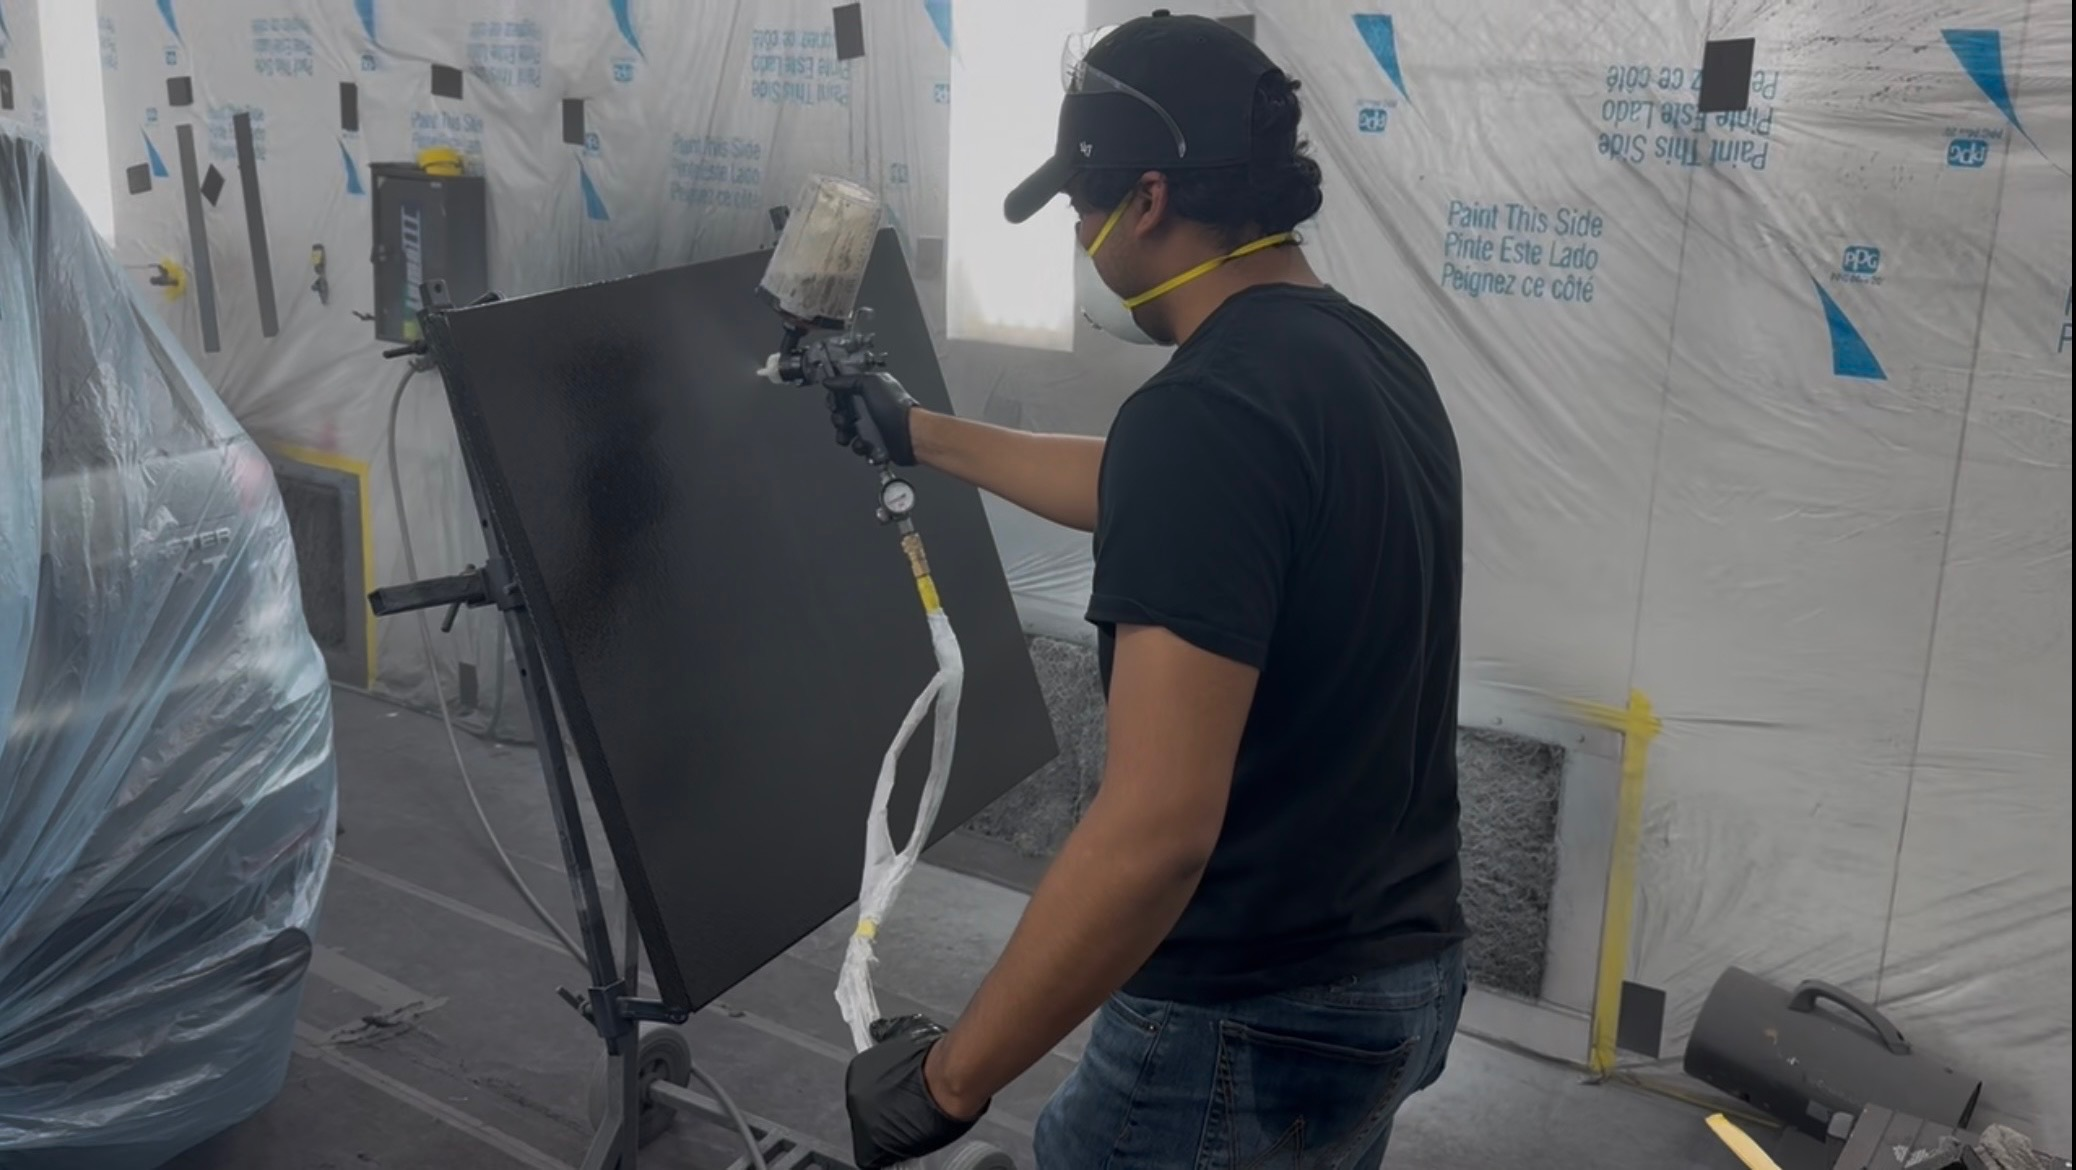
\includegraphics[
        width=2.35in,
        height=1.40in,
        keepaspectratio
    ]{spraying_topcoat}
};
\draw[RuleGray,line width=0.55pt,rounded corners=4pt]
    ($(current page.north west)+(3.10in,-1.91in)$)
    rectangle
    ($(current page.north west)+(5.65in,-3.40in)$);

% Image 3
\node[anchor=center,inner sep=0pt]
at ($(current page.north west)+(7.045in,-2.655in)$)
{
    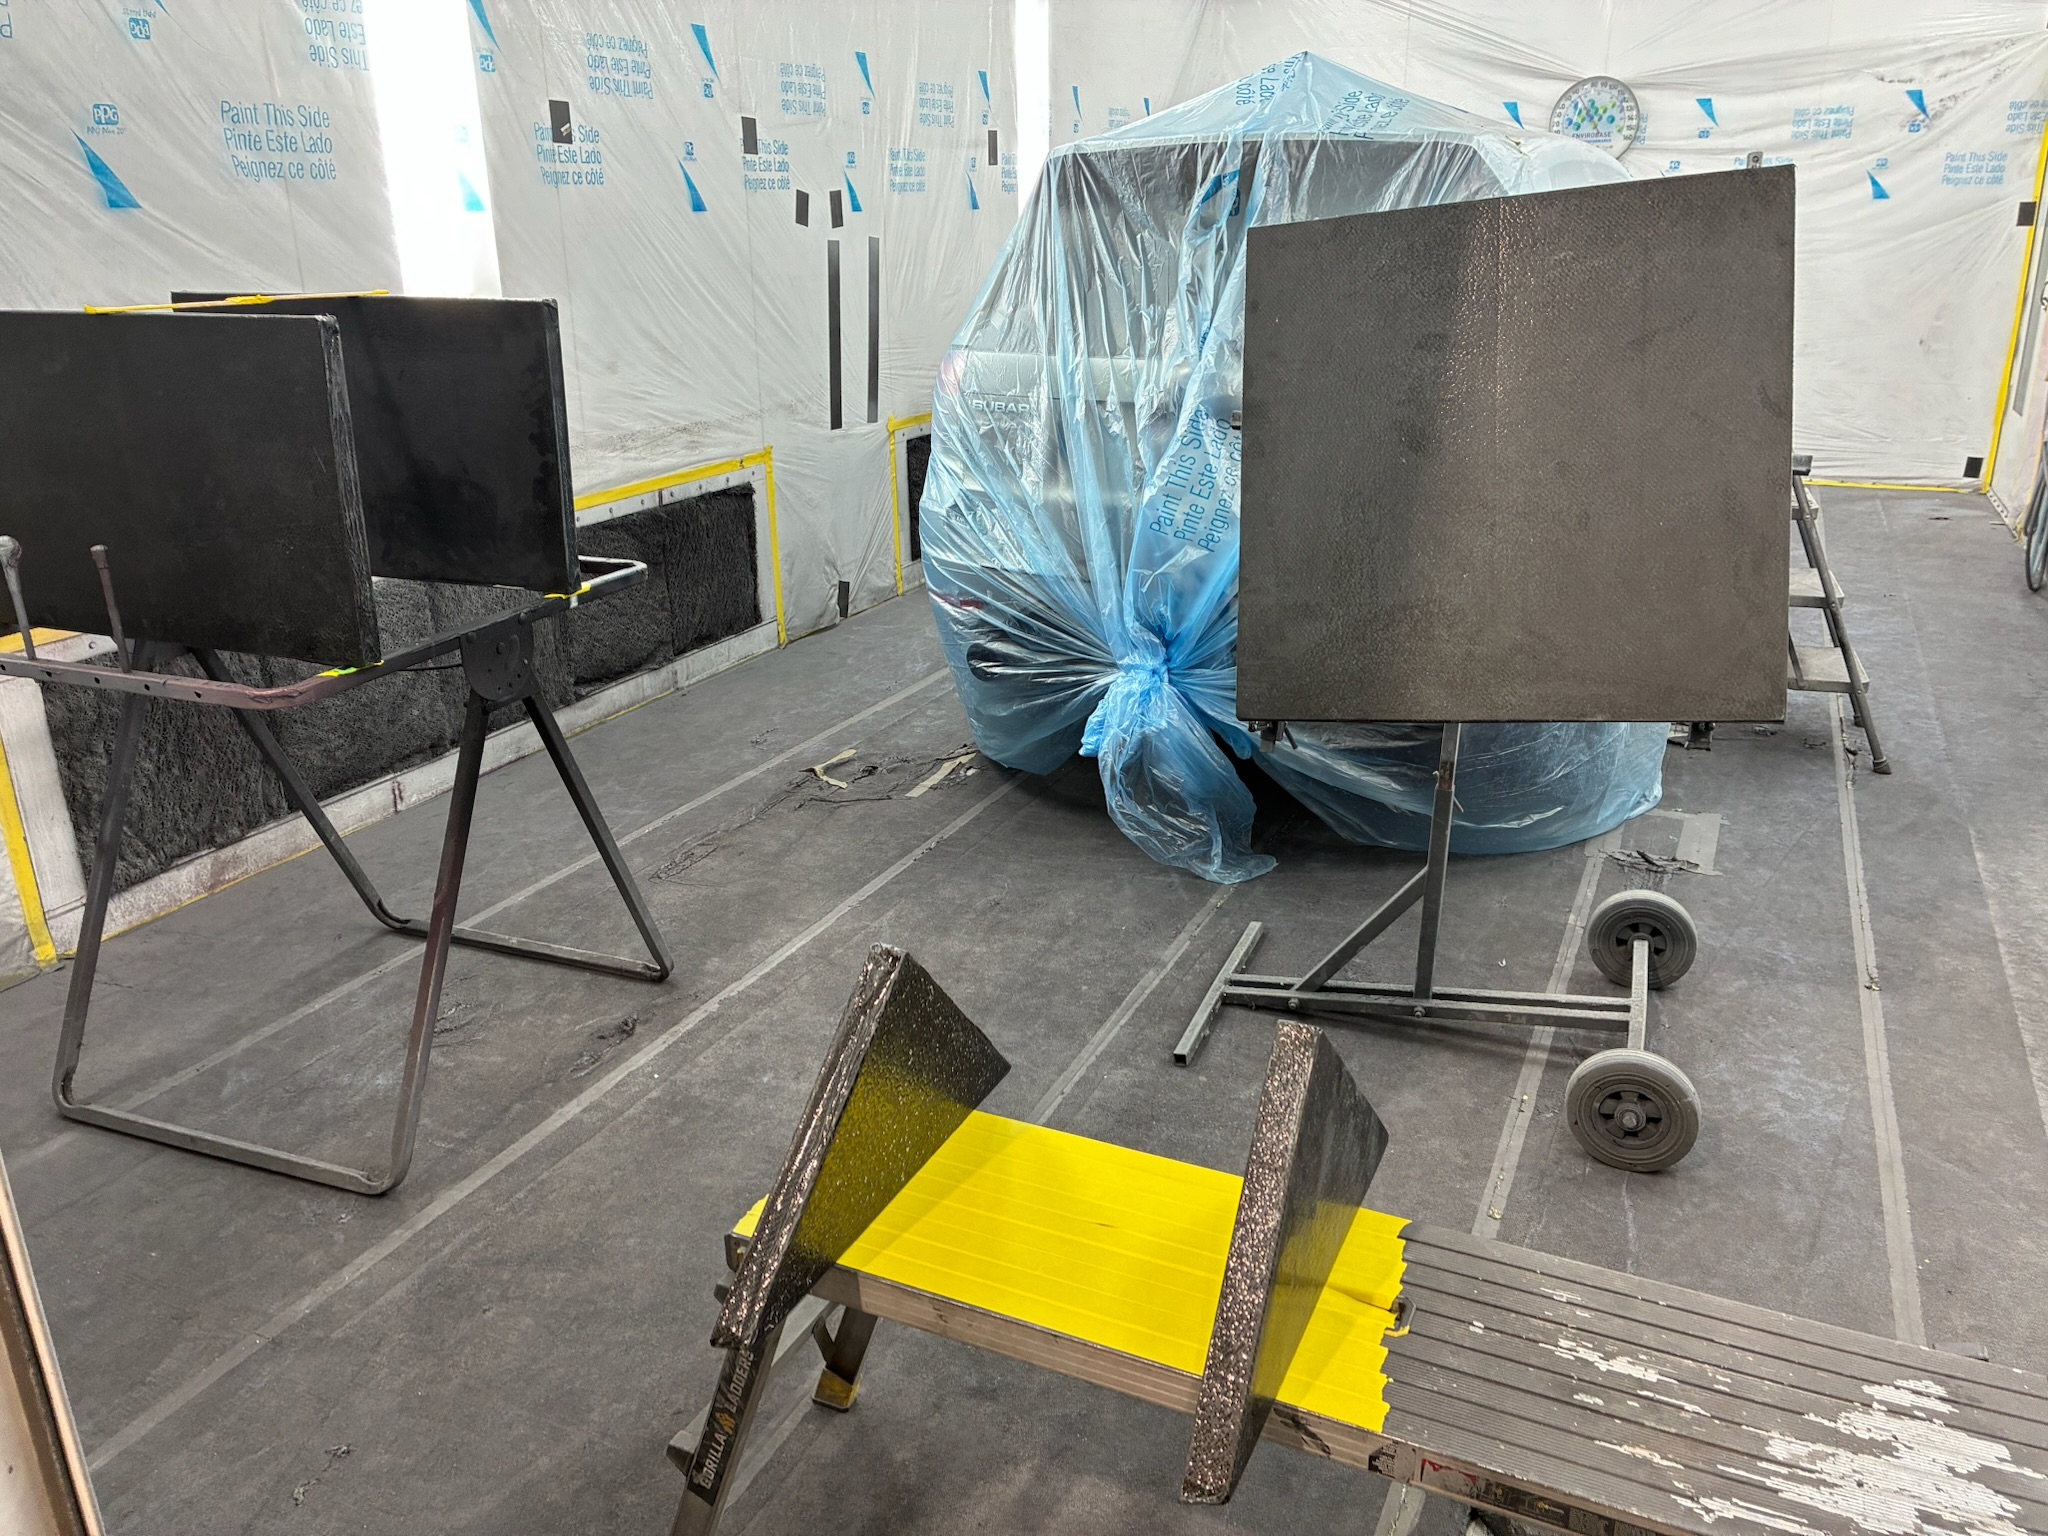
\includegraphics[
        width=2.35in,
        height=1.40in,
        keepaspectratio
    ]{topcoat_setup_apparatus}
};
\draw[RuleGray,line width=0.55pt,rounded corners=4pt]
    ($(current page.north west)+(5.77in,-1.91in)$)
    rectangle
    ($(current page.north west)+(8.32in,-3.40in)$);

% Image 4
\node[anchor=center,inner sep=0pt]
at ($(current page.north west)+(9.50in,-2.655in)$)
{
    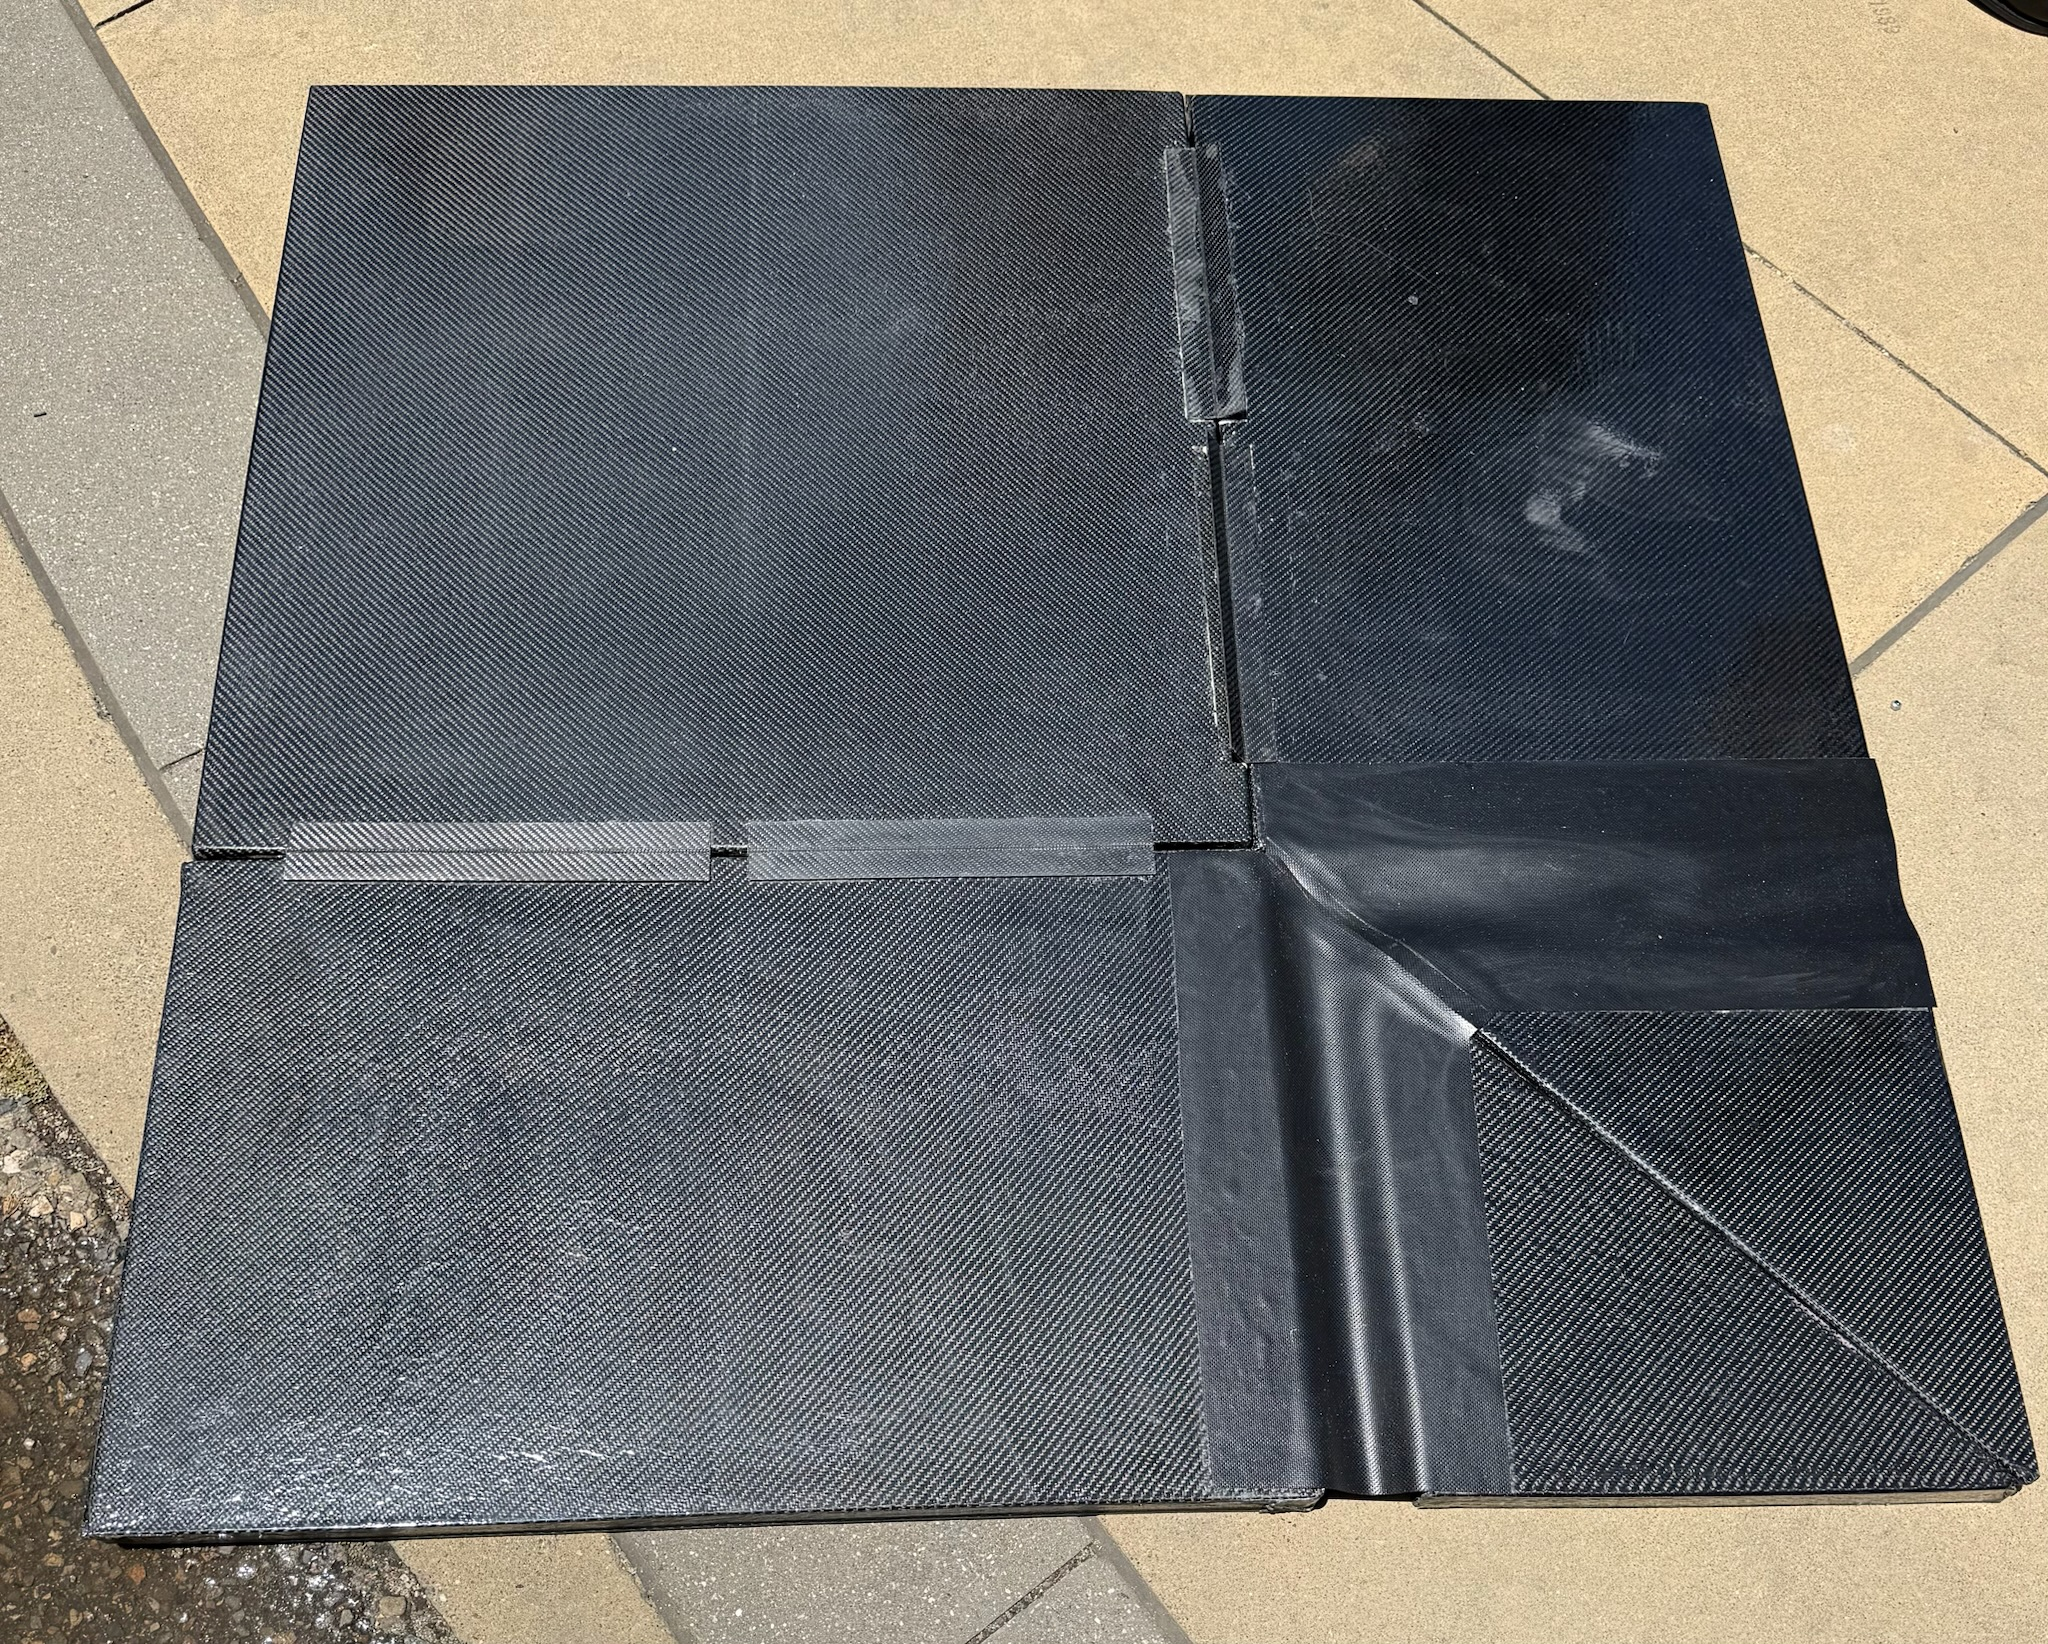
\includegraphics[
        width=2.35in,
        height=1.40in,
        keepaspectratio
    ]{refined_final_toro_cover_partial_carbon_model}
};
\draw[RuleGray,line width=0.55pt,rounded corners=4pt]
    ($(current page.north west)+(8.44in,-1.91in)$)
    rectangle
    ($(current page.north east)+(-0.42in,-3.40in)$);

% Captions
\node[anchor=north,text=Muted,font=\sffamily\fontsize{6.7}{7.3}\selectfont]
at ($(current page.north west)+(1.705in,-3.45in)$)
{Topcoat material preparation};

\node[anchor=north,text=Muted,font=\sffamily\fontsize{6.7}{7.3}\selectfont]
at ($(current page.north west)+(4.375in,-3.45in)$)
{Automotive-booth topcoat application};

\node[anchor=north,text=Muted,font=\sffamily\fontsize{6.7}{7.3}\selectfont]
at ($(current page.north west)+(7.045in,-3.45in)$)
{Coated panels drying after application};

\node[anchor=north,text=Muted,font=\sffamily\fontsize{6.7}{7.3}\selectfont]
at ($(current page.north west)+(9.50in,-3.45in)$)
{Partial carbon manufacturing model};

% Environmental rationale
\fill[SoftGold,rounded corners=4pt]
    ($(current page.north west)+(0.43in,-3.73in)$)
    rectangle
    ($(current page.north east)+(-0.42in,-4.76in)$);

\node[
    anchor=north west,
    align=left,
    text width=9.75in,
    text=Ink,
    font=\fontsize{7.05}{8.25}\selectfont
]
at ($(current page.north west)+(0.65in,-3.89in)$)
{
Because the sponsor required a carbon-fiber cover for outdoor use near chlorinated water,
environmental protection became a functional requirement rather than a cosmetic finish.
I selected and personally sprayed a UV-resistant Sunshield topcoat to seal minor laminate
porosity, reduce moisture ingress, preserve the carbon appearance, limit UV degradation of
the epoxy matrix, and isolate the composite surface from nearby metallic hardware.
};

% Results title
\node[
    anchor=north west,
    text=DeepGreen,
    font=\sffamily\bfseries\fontsize{8.0}{8.7}\selectfont
]
at ($(current page.north west)+(0.43in,-4.94in)$)
{FUNCTIONAL PROTOTYPE RESULTS};

% ------------------------------------------------------------
% Matched lower panels — larger type and improved allocation
% ------------------------------------------------------------

% Left results panel
\fill[SoftGreen,rounded corners=5pt]
    ($(current page.north west)+(0.43in,-5.22in)$)
    rectangle
    ($(current page.north west)+(5.98in,-7.39in)$);

\draw[RuleGray,line width=0.65pt,rounded corners=5pt]
    ($(current page.north west)+(0.43in,-5.22in)$)
    rectangle
    ($(current page.north west)+(5.98in,-7.39in)$);

\fill[DeepGreen,rounded corners=5pt]
    ($(current page.north west)+(0.43in,-5.22in)$)
    rectangle
    ($(current page.north west)+(5.98in,-5.58in)$);

\fill[DeepGreen]
    ($(current page.north west)+(0.43in,-5.40in)$)
    rectangle
    ($(current page.north west)+(5.98in,-5.58in)$);

\node[anchor=west,text=white,
      font=\sffamily\bfseries\fontsize{7.0}{7.6}\selectfont]
at ($(current page.north west)+(0.66in,-5.40in)$)
{SPECIFICATION};

\node[anchor=west,text=white,
      font=\sffamily\bfseries\fontsize{7.0}{7.6}\selectfont]
at ($(current page.north west)+(3.02in,-5.40in)$)
{RESULT};

\node[anchor=east,text=white,
      font=\sffamily\bfseries\fontsize{7.0}{7.6}\selectfont]
at ($(current page.north west)+(5.55in,-5.40in)$)
{STATUS};

\node[
    anchor=north west,
    align=left,
    text width=2.15in,
    text=Ink,
    font=\bfseries\fontsize{7.15}{8.55}\selectfont
]
at ($(current page.north west)+(0.66in,-5.72in)$)
{
Deployment time\\[3.4pt]
Removal time\\[3.4pt]
Single-user operation\\[3.4pt]
Single-side operation\\[3.4pt]
Deployment steps\\[3.4pt]
Removal steps\\[3.4pt]
Weight\\[3.4pt]
Folded storage
};

\node[
    anchor=north west,
    align=left,
    text width=1.45in,
    text=Ink,
    font=\fontsize{7.15}{8.55}\selectfont
]
at ($(current page.north west)+(3.02in,-5.72in)$)
{
25.51 seconds\\[3.4pt]
37.22 seconds\\[3.4pt]
100\% successful\\[3.4pt]
75\% successful\\[3.4pt]
6.4 average\\[3.4pt]
9 average\\[3.4pt]
17 lb\\[3.4pt]
2.9' x 2.9' x 1.7'
};

\node[
    anchor=north east,
    align=right,
    text width=1.05in,
    text=DeepGreen,
    font=\sffamily\bfseries\fontsize{7.05}{8.55}\selectfont
]
at ($(current page.north west)+(5.55in,-5.72in)$)
{
PASS\\[3.4pt]
PASS\\[3.4pt]
PASS\\[3.4pt]
NEAR TARGET\\[3.4pt]
PASS\\[3.4pt]
PASS\\[3.4pt]
NEAR TARGET\\[3.4pt]
PASS
};

% Right takeaways panel — widened for easier reading
\fill[SoftGreen,rounded corners=5pt]
    ($(current page.north west)+(6.14in,-5.22in)$)
    rectangle
    ($(current page.north east)+(-0.42in,-7.39in)$);

\draw[RuleGray,line width=0.65pt,rounded corners=5pt]
    ($(current page.north west)+(6.14in,-5.22in)$)
    rectangle
    ($(current page.north east)+(-0.42in,-7.39in)$);

\fill[DeepGreen,rounded corners=5pt]
    ($(current page.north west)+(6.14in,-5.22in)$)
    rectangle
    ($(current page.north east)+(-0.42in,-5.58in)$);

\fill[DeepGreen]
    ($(current page.north west)+(6.14in,-5.40in)$)
    rectangle
    ($(current page.north east)+(-0.42in,-5.58in)$);

\node[anchor=west,text=white,
      font=\sffamily\bfseries\fontsize{7.1}{7.7}\selectfont]
at ($(current page.north west)+(6.38in,-5.40in)$)
{ENGINEERING TAKEAWAYS};

\node[
    anchor=north west,
    align=left,
    text width=4.02in,
    text=Ink,
    font=\fontsize{6.75}{7.85}\selectfont
]
at ($(current page.north west)+(6.38in,-5.72in)$)
{
\textbf{Manufacturing first.}
Composite manufacturing constraints should guide the product architecture from the beginning.\\[4.5pt]
\textbf{Prioritize deliberately.}
Competing requirements must be balanced intentionally instead of maximizing every objective.\\[4.5pt]
\textbf{Lead through the process.}
Clear procedures, calm communication, and respect for teammates' strengths were essential during fabrication.\\[4.5pt]
\textbf{Next iteration.}
Reduce weight, refine the fabric-hinge fold lines, and improve panel-edge clearance.
};

% Compact concluding pathway
\node[
    anchor=center,
    align=center,
    text=PolyGold,
    font=\sffamily\bfseries\fontsize{6.3}{6.9}\selectfont
]
at ($(current page.north)+(3.06in,-7.18in)$)
{PROTOTYPE \faArrowRight\ DESIGN REFINEMENT
\faArrowRight\ REPEATABLE MANUFACTURING
\faArrowRight\ PRODUCT};

% Validation resources
\node[
    anchor=north,
    align=center,
    text=DeepGreen,
    font=\sffamily\bfseries\fontsize{6.6}{7.2}\selectfont
]
at ($(current page.north)+(0,-7.58in)$)
{\href{\ToroDeploymentLink}{\faPlayCircle\ DEPLOYMENT}
\hspace{18pt}
\href{\ToroRemovalLink}{\faPlayCircle\ REMOVAL / FOLDING}
\hspace{18pt}
\href{\ToroPosterLink}{\faFilePdf\ EXPO POSTER}
\hspace{18pt}
\href{\ToroReportLink}{\faFilePdf\ FINAL REPORT}};

% Footer
\node[
    anchor=south west,
    text=white,
    font=\sffamily\bfseries\fontsize{7.1}{7.7}\selectfont
]
at ($(current page.south west)+(0.42in,0.17in)$)
{\faArrowLeft\ MANUFACTURING-DRIVEN DESIGN};

\node[
    anchor=south,
    text=white,
    font=\sffamily\fontsize{7.0}{7.6}\selectfont
]
at ($(current page.south)+(0,0.17in)$)
{TORO COVER \hspace{6pt} 3 / 3};

\node[
    anchor=south east,
    text=white,
    font=\sffamily\bfseries\fontsize{7.1}{7.7}\selectfont
]
at ($(current page.south east)+(-0.42in,0.17in)$)
{NEXT PROJECT \faArrowRight};

\end{tikzpicture}
\input{paddle}
\clearpage
.
% 2. In main.tex, place 
% ============================================================
% TORO COVER — THREE-PAGE PORTFOLIO CASE STUDY
% Pages 3–5 of the complete portfolio
%
% IMPORTANT:
% 1. This file must NOT contain \documentclass, \begin{document},
%    \end{document}, or \input{toro}.
% 2. In main.tex, place \input{toro} before \end{document}.
% 3. Image references use the original Overleaf base filenames
%    without extensions.
% ============================================================



% ============================================================
% CLICKABLE PROJECT RESOURCES
% All links use the exact Google Drive resources supplied.
% ============================================================
\providecommand{\ToroDrawingLink}{https://drive.google.com/file/d/1A7-7wMnRNLuQDaTgxeuUCBsGNqyXzOGV/view?usp=sharing}
\providecommand{\ToroDimensionsLink}{https://drive.google.com/file/d/13sw3BNJvE8GdzlRffxoF2n5r9Gzxide7/view?usp=sharing}
\providecommand{\ToroProblemLink}{https://drive.google.com/file/d/1zHtl8zrb13F1yeN74ptawpfS5UM_xsuw/view?usp=drive_link}
\providecommand{\ToroReportLink}{https://drive.google.com/file/d/1ULZ-P46lFsC2x29ZfmRVIKgYnr9o8hMt/view?usp=drive_link}
\providecommand{\ToroPosterLink}{https://drive.google.com/file/d/1vKiKaJUcHQb_db-FkZnRF6EvtuM4hKyS/view?usp=drive_link}
\providecommand{\ToroDeploymentLink}{https://drive.google.com/file/d/1XJx34o80_mZPTl7xy93HtWAgtS3ThhvY/view?usp=drive_link}
\providecommand{\ToroRemovalLink}{https://drive.google.com/file/d/1O7xYeyB67NUwT-j1B1HeiCcHnZDYjk6_/view?usp=drive_link}

% ============================================================
% PAGE 1 — PROJECT OVERVIEW, OWNERSHIP, AND ARCHITECTURE
% ============================================================

\clearpage
\thispagestyle{empty}
\hypertarget{toro}{}
\null

\begin{tikzpicture}[remember picture,overlay]

% Background
\fill[white]
    (current page.south west)
    rectangle
    (current page.north east);

% Page bars
\fill[DeepGreen]
    (current page.north west)
    rectangle
    ($(current page.north east)+(0,-0.095in)$);

\fill[PolyGold]
    ($(current page.north west)+(0,-0.095in)$)
    rectangle
    ($(current page.north east)+(0,-0.14in)$);

\fill[DeepGreen]
    (current page.south west)
    rectangle
    ($(current page.south east)+(0,0.36in)$);

\fill[PolyGold]
    ($(current page.south west)+(0,0.36in)$)
    rectangle
    ($(current page.south east)+(0,0.405in)$);

% Header
\node[
    anchor=north west,
    text=PolyGold,
    font=\sffamily\bfseries\fontsize{8.1}{8.7}\selectfont
]
at ($(current page.north west)+(0.42in,-0.39in)$)
{01 COMPOSITES \hspace{5pt}/\hspace{5pt} PROJECT 01};

\node[
    anchor=north west,
    text=DeepGreen,
    font=\bfseries\fontsize{23.5}{24.5}\selectfont
]
at ($(current page.north west)+(0.40in,-0.67in)$)
{TORO CARBON FIBER SAFETY COVER};

\node[
    anchor=north west,
    text=Muted,
    font=\sffamily\fontsize{8.4}{9.2}\selectfont
]
at ($(current page.north west)+(0.42in,-1.12in)$)
{Cal Poly Composites Laboratory \hspace{7pt}\textbullet\hspace{7pt}
Team Project \hspace{7pt}\textbullet\hspace{7pt}
Fall--Spring 2026 \hspace{7pt}\textbullet\hspace{7pt}
San Luis Obispo, California};

\fill[PolyGold]
    ($(current page.north west)+(0.42in,-1.37in)$)
    rectangle
    ($(current page.north west)+(6.1in,-1.325in)$);

% Challenge text
\node[
    anchor=north west,
    text=DeepGreen,
    font=\sffamily\bfseries\fontsize{8.1}{8.8}\selectfont
]
at ($(current page.north west)+(0.43in,-1.61in)$)
{THE CHALLENGE};

\node[
    anchor=north west,
    align=left,
    text width=4.47in,
    text=Ink,
    font=\fontsize{8.05}{9.65}\selectfont
]
at ($(current page.north west)+(0.43in,-1.84in)$)
{
Develop a lightweight cover for a 6 ft by 6 ft in-ground spa
that could be deployed by one person, stored compactly,
provide insulation, resist a poolside environment, and maintain
a refined appearance. The sponsor supplied an ambitious but
intentionally broad project statement, requiring the team to
define the product architecture, priorities, manufacturing
strategy, and realistic path toward future commercialization.
};

% Role box
\fill[SoftGold,rounded corners=5pt]
    ($(current page.north west)+(0.42in,-2.88in)$)
    rectangle
    ($(current page.north west)+(4.98in,-4.58in)$);

\fill[PolyGold]
    ($(current page.north west)+(0.42in,-2.88in)$)
    rectangle
    ($(current page.north west)+(0.52in,-4.58in)$);

\node[
    anchor=north west,
    text=DeepGreen,
    font=\sffamily\bfseries\fontsize{8.1}{8.8}\selectfont
]
at ($(current page.north west)+(0.66in,-3.02in)$)
{MY ROLE — DESIGN \& MANUFACTURING LEAD};

\node[
    anchor=north west,
    align=left,
    text width=4.02in,
    text=Ink,
    font=\fontsize{7.05}{8.15}\selectfont
]
at ($(current page.north west)+(0.66in,-3.27in)$)
{
\textbullet\ Modeled every custom part and the complete assembly\\[1.5pt]
\textbullet\ Produced the engineering drawing package independently\\[1.5pt]
\textbullet\ Developed the composite-panel manufacturing process\\[1.5pt]
\textbullet\ Created all waterjet DXFs and manufacturing geometry\\[1.5pt]
\textbullet\ Trained teammates in wet layup and vacuum bagging\\[1.5pt]
\textbullet\ Presented feasibility, scope, and tradeoffs to the sponsor
};

% Large deployed foam-model image
\node[anchor=center,inner sep=0pt]
at ($(current page.north west)+(8.00in,-3.04in)$)
{
    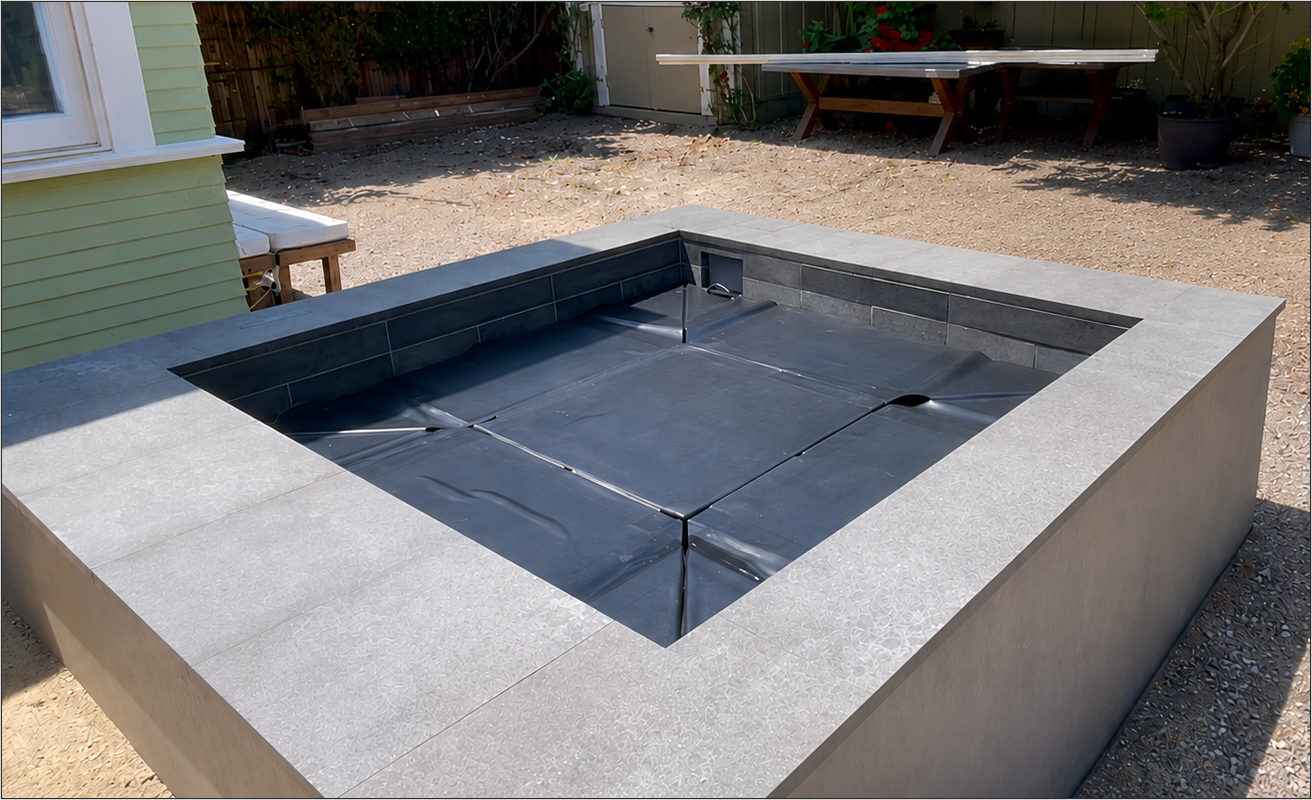
\includegraphics[
        width=5.55in,
        height=2.78in,
        keepaspectratio
    ]{deployed_functional_prototype}
};

\draw[DeepGreen,line width=0.8pt,rounded corners=7pt]
    ($(current page.north west)+(5.16in,-1.61in)$)
    rectangle
    ($(current page.north east)+(-0.42in,-4.47in)$);

\node[
    anchor=north west,
    text=Muted,
    font=\sffamily\fontsize{6.2}{6.9}\selectfont
]
at ($(current page.north west)+(5.18in,-4.54in)$)
{Functional foam model deployed over the sponsor's in-ground spa.};

% Image-strip title
\node[
    anchor=north west,
    text=DeepGreen,
    font=\sffamily\bfseries\fontsize{8.1}{8.8}\selectfont
]
at ($(current page.north west)+(0.43in,-4.78in)$)
{PRODUCT DEVELOPMENT AND FINAL ARCHITECTURE};

% Five-image development strip — CAD-first sequence
% Image 1: topside CAD
\node[anchor=center,inner sep=0pt]
at ($(current page.north west)+(1.47in,-5.73in)$)
{
    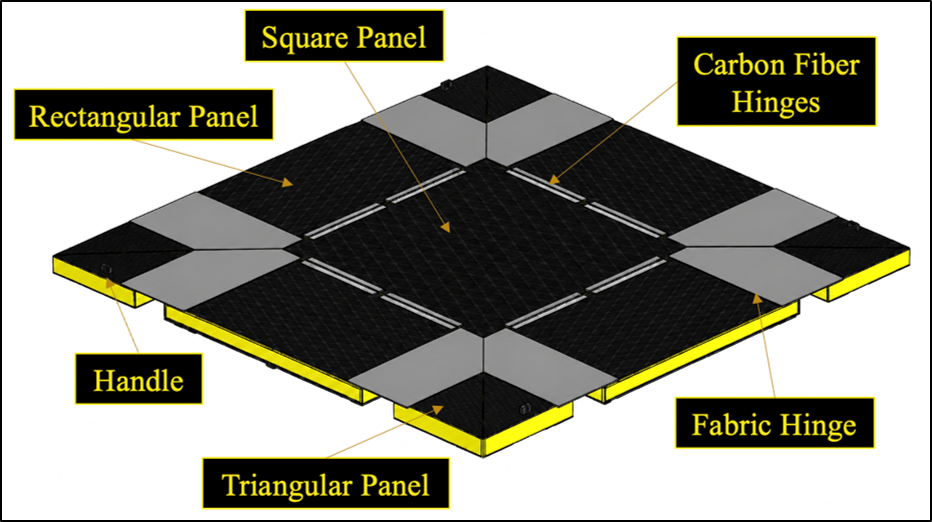
\includegraphics[
        width=1.92in,
        height=1.30in,
        keepaspectratio
    ]{Toro_Cover_topside_Cad}
};
\draw[RuleGray,line width=0.55pt,rounded corners=4pt]
    ($(current page.north west)+(0.43in,-5.04in)$)
    rectangle
    ($(current page.north west)+(2.51in,-6.43in)$);

% Image 2: underside CAD
\node[anchor=center,inner sep=0pt]
at ($(current page.north west)+(3.66in,-5.73in)$)
{
    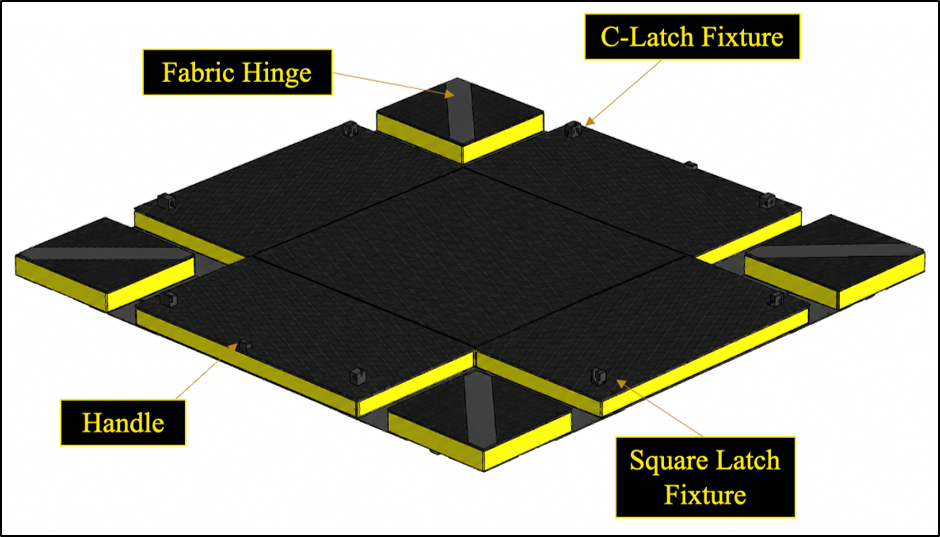
\includegraphics[
        width=1.92in,
        height=1.30in,
        keepaspectratio
    ]{toro_cover_underside_cad}
};
\draw[RuleGray,line width=0.55pt,rounded corners=4pt]
    ($(current page.north west)+(2.62in,-5.04in)$)
    rectangle
    ($(current page.north west)+(4.70in,-6.43in)$);

% Image 3: folded CAD
\node[anchor=center,inner sep=0pt]
at ($(current page.north west)+(5.85in,-5.73in)$)
{
    \includegraphics[
        width=1.92in,
        height=1.30in,
        keepaspectratio
    ]{\detokenize{Toro_Cover_folded Configuration}}
};
\draw[RuleGray,line width=0.55pt,rounded corners=4pt]
    ($(current page.north west)+(4.81in,-5.04in)$)
    rectangle
    ($(current page.north west)+(6.89in,-6.43in)$);

% Image 4: dual-use product concept
\node[anchor=center,inner sep=0pt]
at ($(current page.north west)+(8.04in,-5.73in)$)
{
    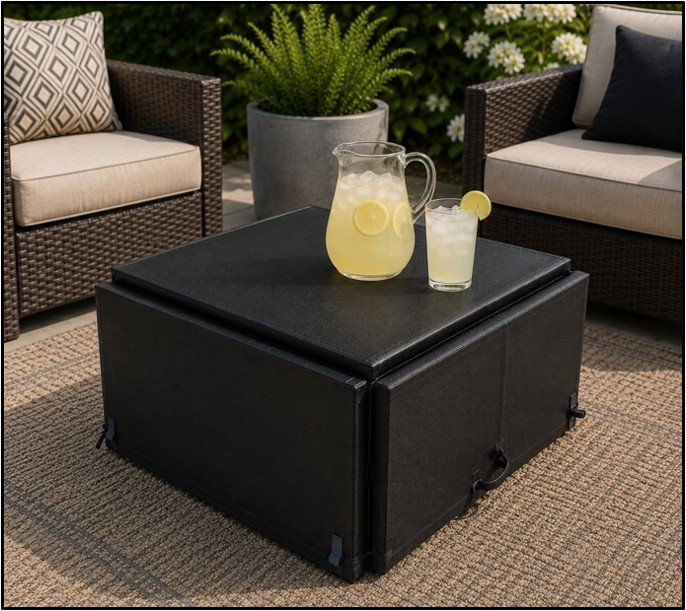
\includegraphics[
        width=1.92in,
        height=1.30in,
        keepaspectratio
    ]{generative_AI_concept_toro_cover_art}
};
\draw[RuleGray,line width=0.55pt,rounded corners=4pt]
    ($(current page.north west)+(7.00in,-5.04in)$)
    rectangle
    ($(current page.north west)+(9.08in,-6.43in)$);

% Image 5: folded foam functional prototype
% The portrait photograph is deliberately clipped to the landscape frame
% so the ottoman fills the card without extending beyond its border.
\begin{scope}
\clip[rounded corners=4pt]
    ($(current page.north west)+(9.19in,-5.04in)$)
    rectangle
    ($(current page.north east)+(-0.43in,-6.43in)$);

% Keep the original image proportions and center it within the existing card.
\node[anchor=center,inner sep=0pt]
at ($(current page.north west)+(9.88in,-5.735in)$)
{
    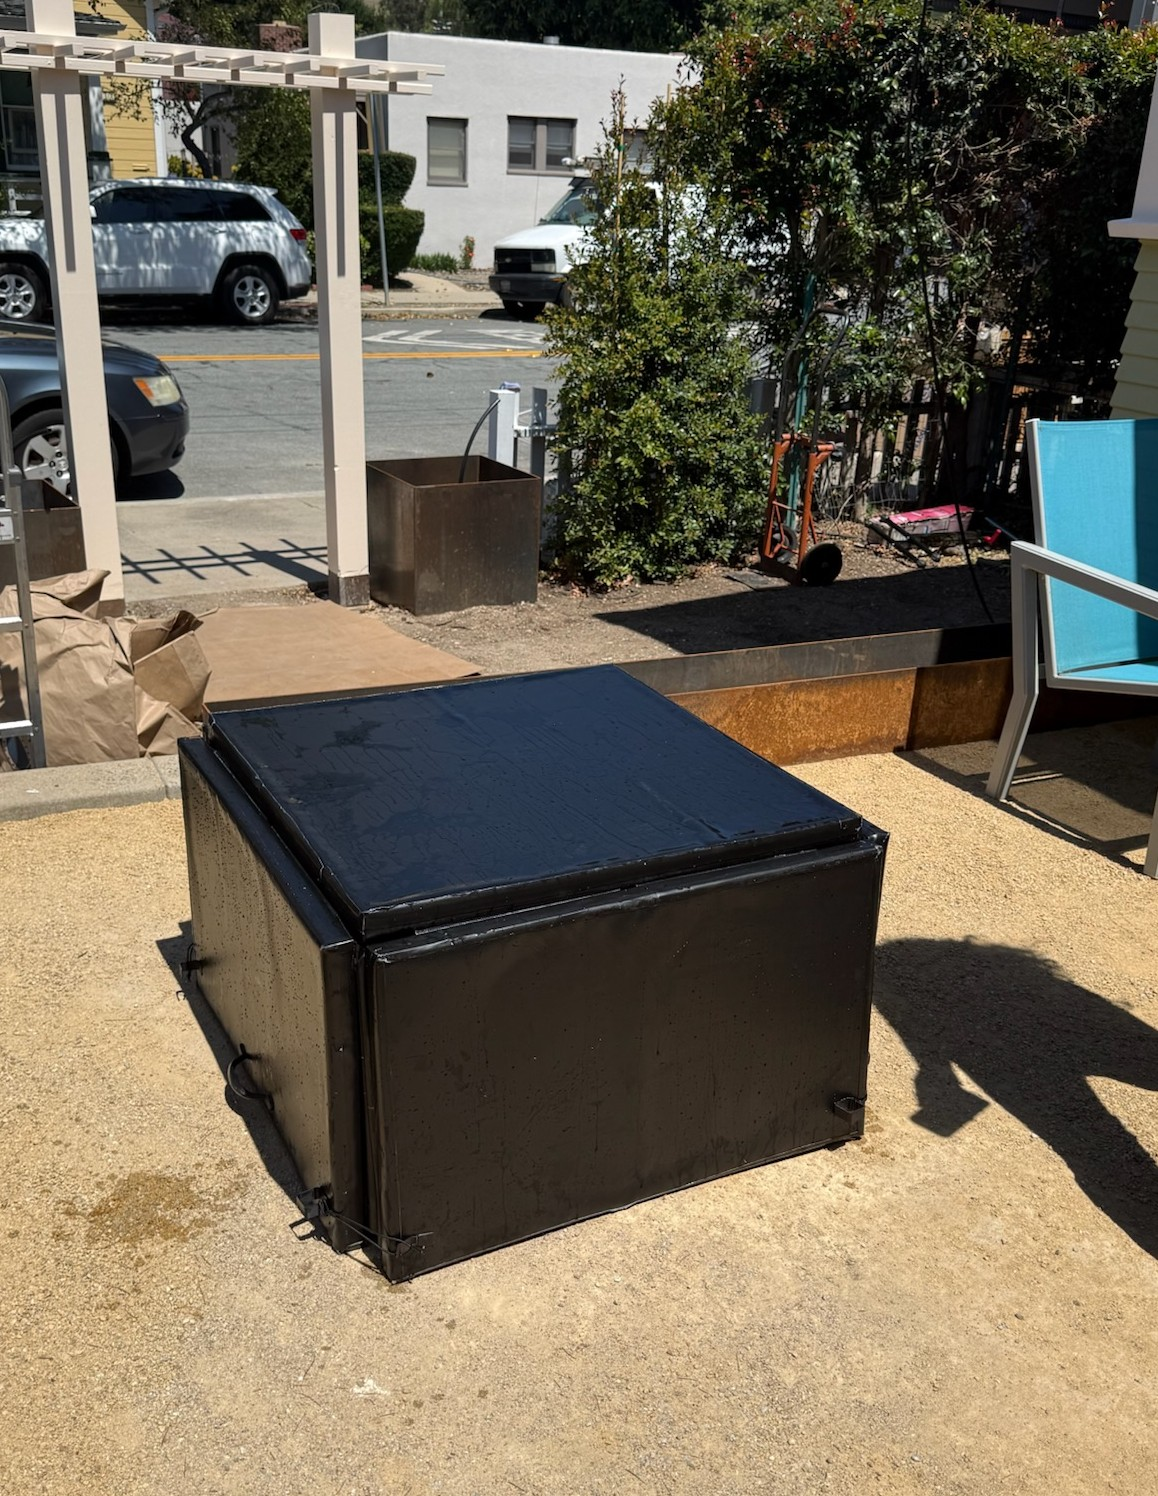
\includegraphics[
        width=1.58in,
        height=1.28in,
        keepaspectratio
    ]{foam_model_folded_backyard_image}
};
\end{scope}

\draw[RuleGray,line width=0.55pt,rounded corners=4pt]
    ($(current page.north west)+(9.19in,-5.04in)$)
    rectangle
    ($(current page.north east)+(-0.43in,-6.43in)$);

% Larger captions
\node[anchor=north,align=center,text width=1.95in,text=Muted,
      font=\sffamily\fontsize{6.8}{7.4}\selectfont]
at ($(current page.north west)+(1.47in,-6.49in)$)
{Topside panel architecture};

\node[anchor=north,align=center,text width=1.95in,text=Muted,
      font=\sffamily\fontsize{6.8}{7.4}\selectfont]
at ($(current page.north west)+(3.66in,-6.49in)$)
{Underside hinge architecture};

\node[anchor=north,align=center,text width=1.95in,text=Muted,
      font=\sffamily\fontsize{6.8}{7.4}\selectfont]
at ($(current page.north west)+(5.85in,-6.49in)$)
{Folded CAD configuration};

\node[anchor=north,align=center,text width=1.95in,text=Muted,
      font=\sffamily\fontsize{6.8}{7.4}\selectfont]
at ($(current page.north west)+(8.04in,-6.49in)$)
{Dual-use product vision};

\node[anchor=north,align=center,text width=1.95in,text=Muted,
      font=\sffamily\fontsize{6.8}{7.4}\selectfont]
at ($(current page.north west)+(9.88in,-6.49in)$)
{Folded foam prototype};

% Page 1 resource bar — centered and non-repeated resources
\fill[Panel,rounded corners=4pt]
    ($(current page.north west)+(0.43in,-7.05in)$)
    rectangle
    ($(current page.north east)+(-0.43in,-7.64in)$);
\draw[RuleGray,line width=0.5pt,rounded corners=4pt]
    ($(current page.north west)+(0.43in,-7.05in)$)
    rectangle
    ($(current page.north east)+(-0.43in,-7.64in)$);

\node[
    anchor=center,
    align=center,
    text=DeepGreen,
    font=\sffamily\bfseries\fontsize{6.9}{7.5}\selectfont
]
at ($(current page.north)+(0,-7.345in)$)
{\href{\ToroDrawingLink}{\faDraftingCompass\ DRAWING PACKAGE}
\hspace{24pt}
\href{\ToroDimensionsLink}{\faImage\ DIMENSION STUDY}
\hspace{24pt}
\href{\ToroProblemLink}{\faFileImage\ PROBLEM STATEMENT}};

% Footer
\node[
    anchor=south west,
    text=white,
    font=\sffamily\bfseries\fontsize{7.1}{7.7}\selectfont
]
at ($(current page.south west)+(0.42in,0.17in)$)
{\hyperlink{composites}{\faArrowLeft\ COMPOSITES}};

\node[
    anchor=south,
    text=white,
    font=\sffamily\fontsize{7.0}{7.6}\selectfont
]
at ($(current page.south)+(0,0.17in)$)
{TORO COVER \hspace{6pt} 1 / 3};

\node[
    anchor=south east,
    text=white,
    font=\sffamily\bfseries\fontsize{7.1}{7.7}\selectfont
]
at ($(current page.south east)+(-0.42in,0.17in)$)
{MANUFACTURING-DRIVEN DESIGN \faArrowRight};

\end{tikzpicture}


% ============================================================
% PAGE 2 — MANUFACTURING-DRIVEN DESIGN
% ============================================================

\clearpage
\thispagestyle{empty}
\hypertarget{toro-manufacturing}{}
\null

\begin{tikzpicture}[remember picture,overlay]

% Background and bars
\fill[white]
    (current page.south west)
    rectangle
    (current page.north east);

\fill[DeepGreen]
    (current page.north west)
    rectangle
    ($(current page.north east)+(0,-0.095in)$);

\fill[PolyGold]
    ($(current page.north west)+(0,-0.095in)$)
    rectangle
    ($(current page.north east)+(0,-0.14in)$);

\fill[DeepGreen]
    (current page.south west)
    rectangle
    ($(current page.south east)+(0,0.36in)$);

\fill[PolyGold]
    ($(current page.south west)+(0,0.36in)$)
    rectangle
    ($(current page.south east)+(0,0.405in)$);

% Header
\node[
    anchor=north west,
    text=PolyGold,
    font=\sffamily\bfseries\fontsize{8.1}{8.7}\selectfont
]
at ($(current page.north west)+(0.42in,-0.39in)$)
{TORO COVER \hspace{5pt}/\hspace{5pt} DESIGN FOR MANUFACTURABILITY};

\node[
    anchor=north west,
    text=DeepGreen,
    font=\bfseries\fontsize{23}{24}\selectfont
]
at ($(current page.north west)+(0.40in,-0.67in)$)
{THE ENVELOPE METHOD};

\node[
    anchor=north west,
    text=Muted,
    font=\sffamily\fontsize{8.7}{9.6}\selectfont
]
at ($(current page.north west)+(0.42in,-1.12in)$)
{A one-layup process developed for unusually thick insulated composite sandwich panels};

\fill[PolyGold]
    ($(current page.north west)+(0.42in,-1.36in)$)
    rectangle
    ($(current page.north west)+(5.30in,-1.315in)$);

% Process explanation
\fill[SoftGold,rounded corners=5pt]
    ($(current page.north west)+(0.42in,-1.61in)$)
    rectangle
    ($(current page.north east)+(-0.42in,-2.90in)$);

\fill[PolyGold]
    ($(current page.north west)+(0.42in,-1.61in)$)
    rectangle
    ($(current page.north west)+(0.52in,-2.90in)$);

\node[
    anchor=north west,
    text=DeepGreen,
    font=\sffamily\bfseries\fontsize{7.9}{8.6}\selectfont
]
at ($(current page.north west)+(0.67in,-1.76in)$)
{PROCESS INNOVATION};

\node[
    anchor=north west,
    align=left,
    text width=9.55in,
    text=Ink,
    font=\fontsize{7.35}{8.75}\selectfont
]
at ($(current page.north west)+(0.67in,-2.02in)$)
{
Weight reduction and insulation were both essential, leading to the selection of an
XPS foam core. Because XPS could not tolerate composite heat-cure temperatures, prepreg
processing was not practical and the panels had to be manufactured by wet layup with a
room-temperature cure. To simplify this process, I waterjet-cut XPS perimeter strips from
excess foam and placed them around each core inside the vacuum enclosure. Under vacuum,
the top and bottom carbon skins met along the panel sides and compressed against this
border, eliminating a separate edge-banding layup and reducing corner pleating.
};

% Workflow title
\node[
    anchor=north west,
    text=DeepGreen,
    font=\sffamily\bfseries\fontsize{8.0}{8.7}\selectfont
]
at ($(current page.north west)+(0.43in,-3.06in)$)
{MANUFACTURING WORKFLOW};

% Row 1 image 1
\node[anchor=center,inner sep=0pt]
at ($(current page.north west)+(2.07in,-4.105in)$)
{
    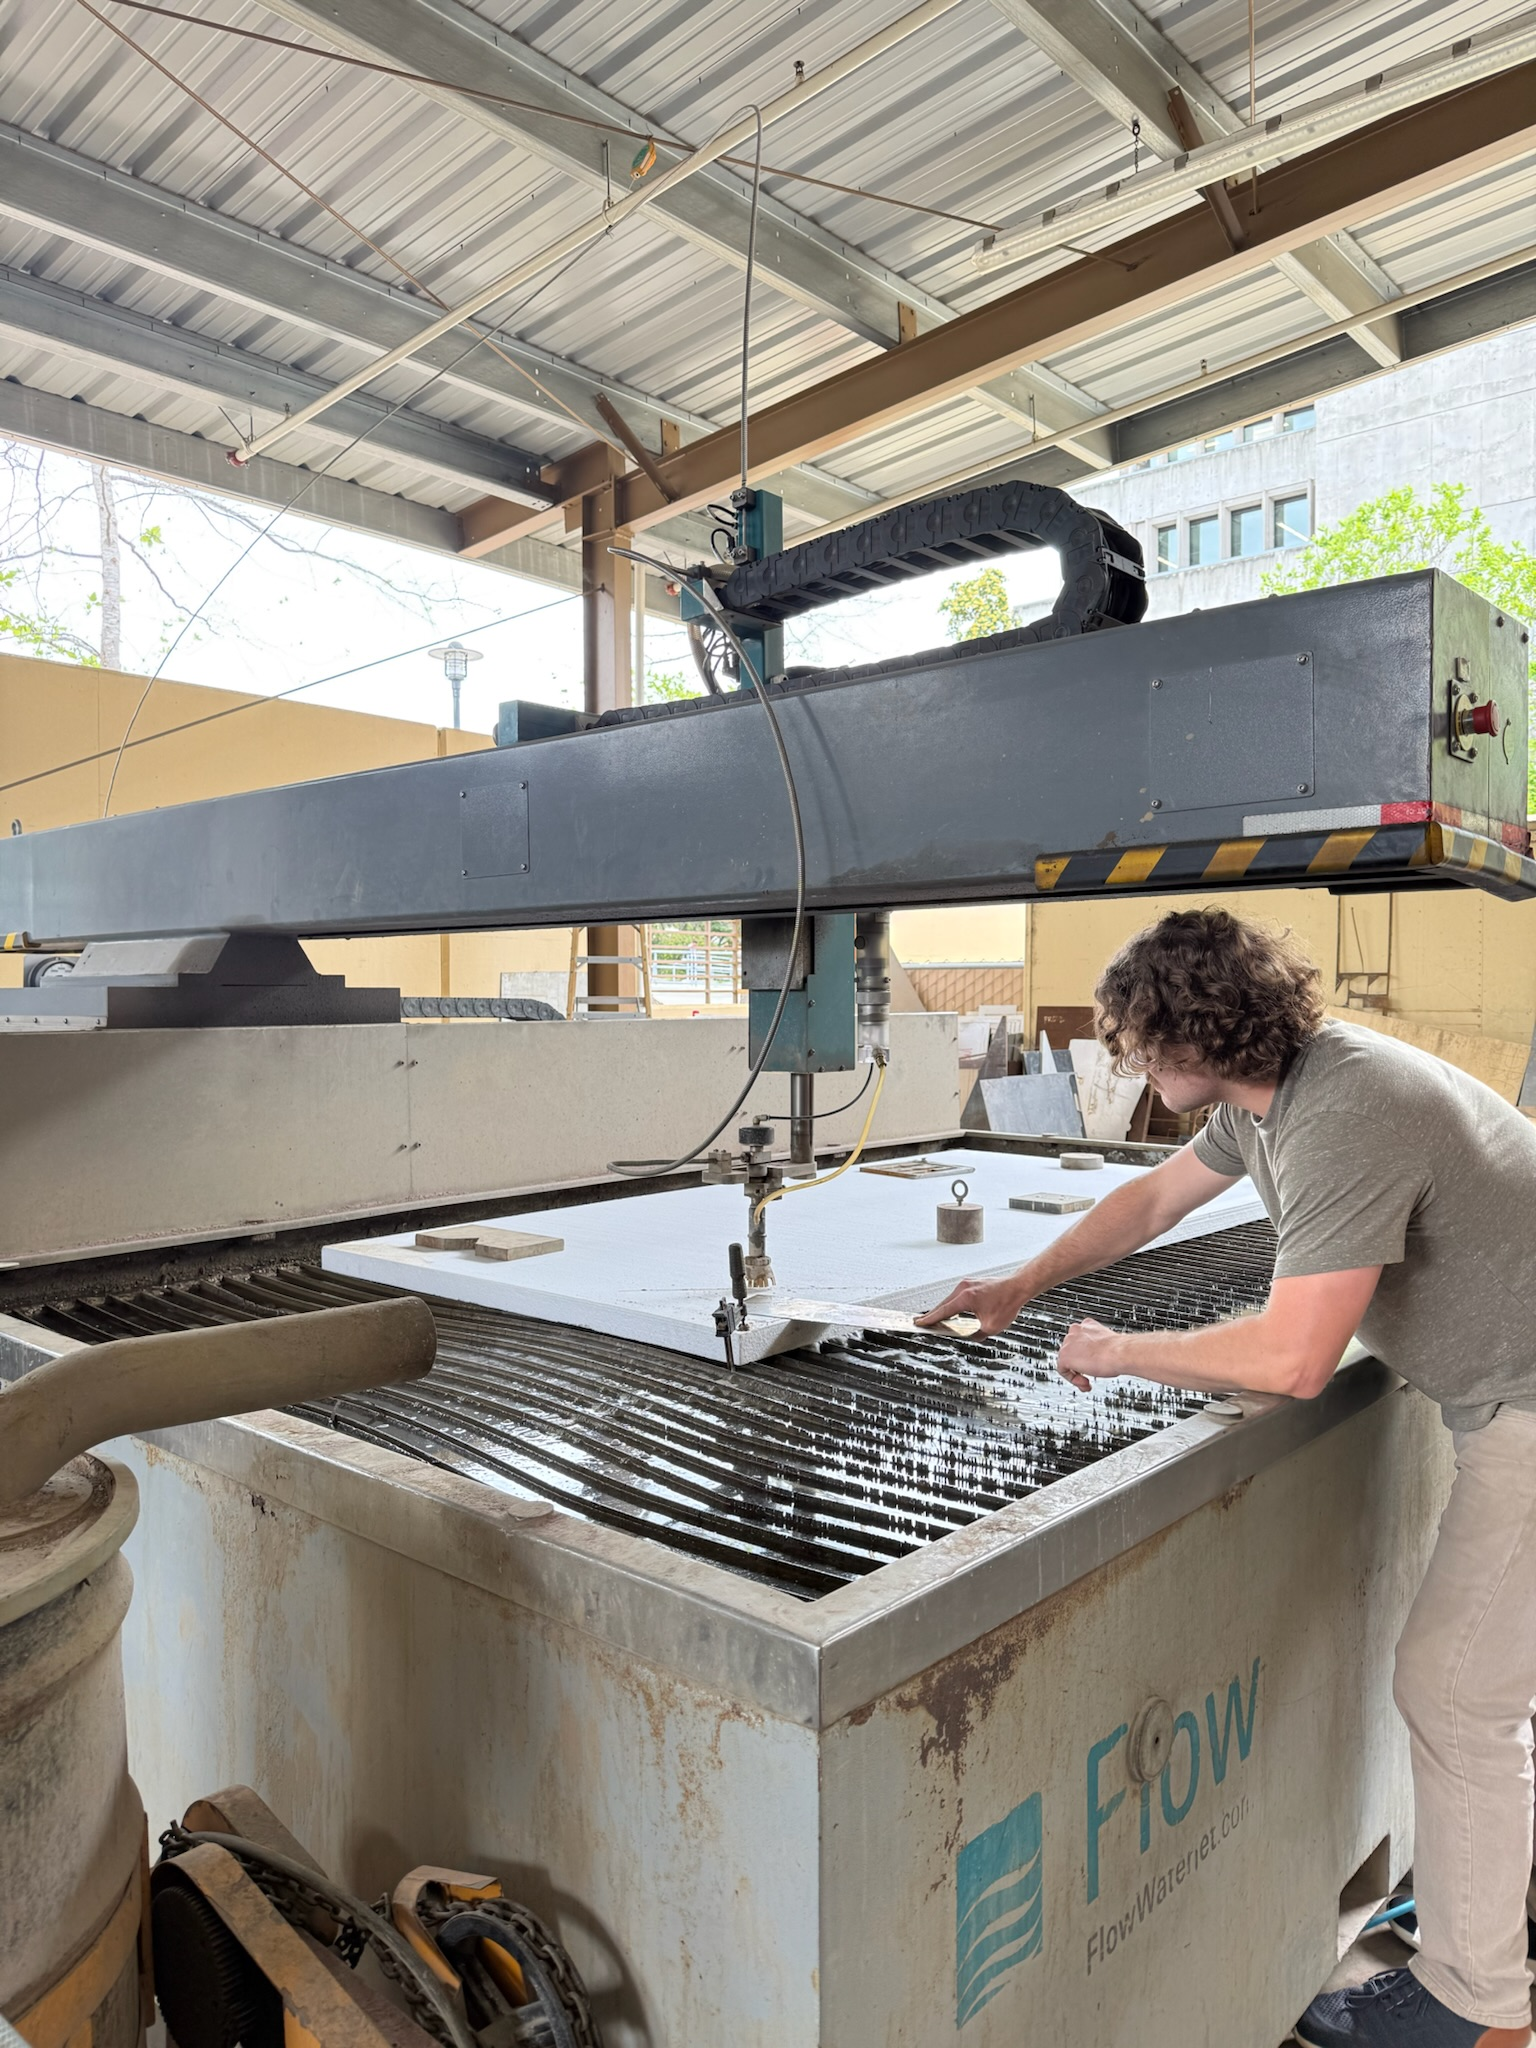
\includegraphics[
        width=3.10in,
        height=1.40in,
        keepaspectratio
    ]{waterjet_foam}
};
\draw[RuleGray,line width=0.55pt,rounded corners=4pt]
    ($(current page.north west)+(0.43in,-3.36in)$)
    rectangle
    ($(current page.north west)+(3.71in,-4.85in)$);

% Row 1 image 2
\node[anchor=center,inner sep=0pt]
at ($(current page.north west)+(5.50in,-4.105in)$)
{
    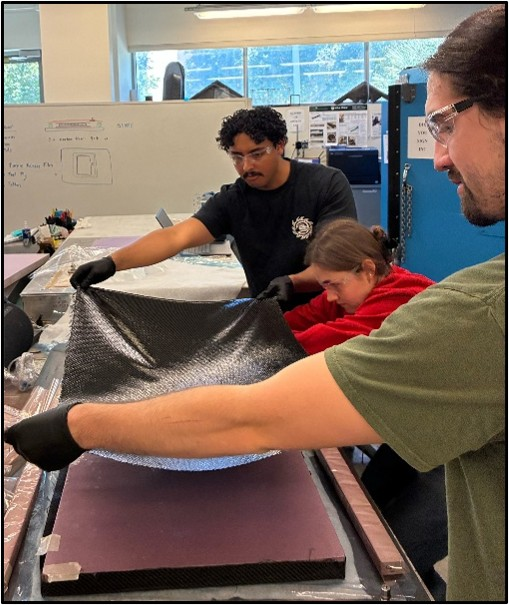
\includegraphics[
        width=3.10in,
        height=1.40in,
        keepaspectratio
    ]{group_layup}
};
\draw[RuleGray,line width=0.55pt,rounded corners=4pt]
    ($(current page.north west)+(3.86in,-3.36in)$)
    rectangle
    ($(current page.north west)+(7.14in,-4.85in)$);

% Row 1 image 3
\node[anchor=center,inner sep=0pt]
at ($(current page.north west)+(8.935in,-4.105in)$)
{
    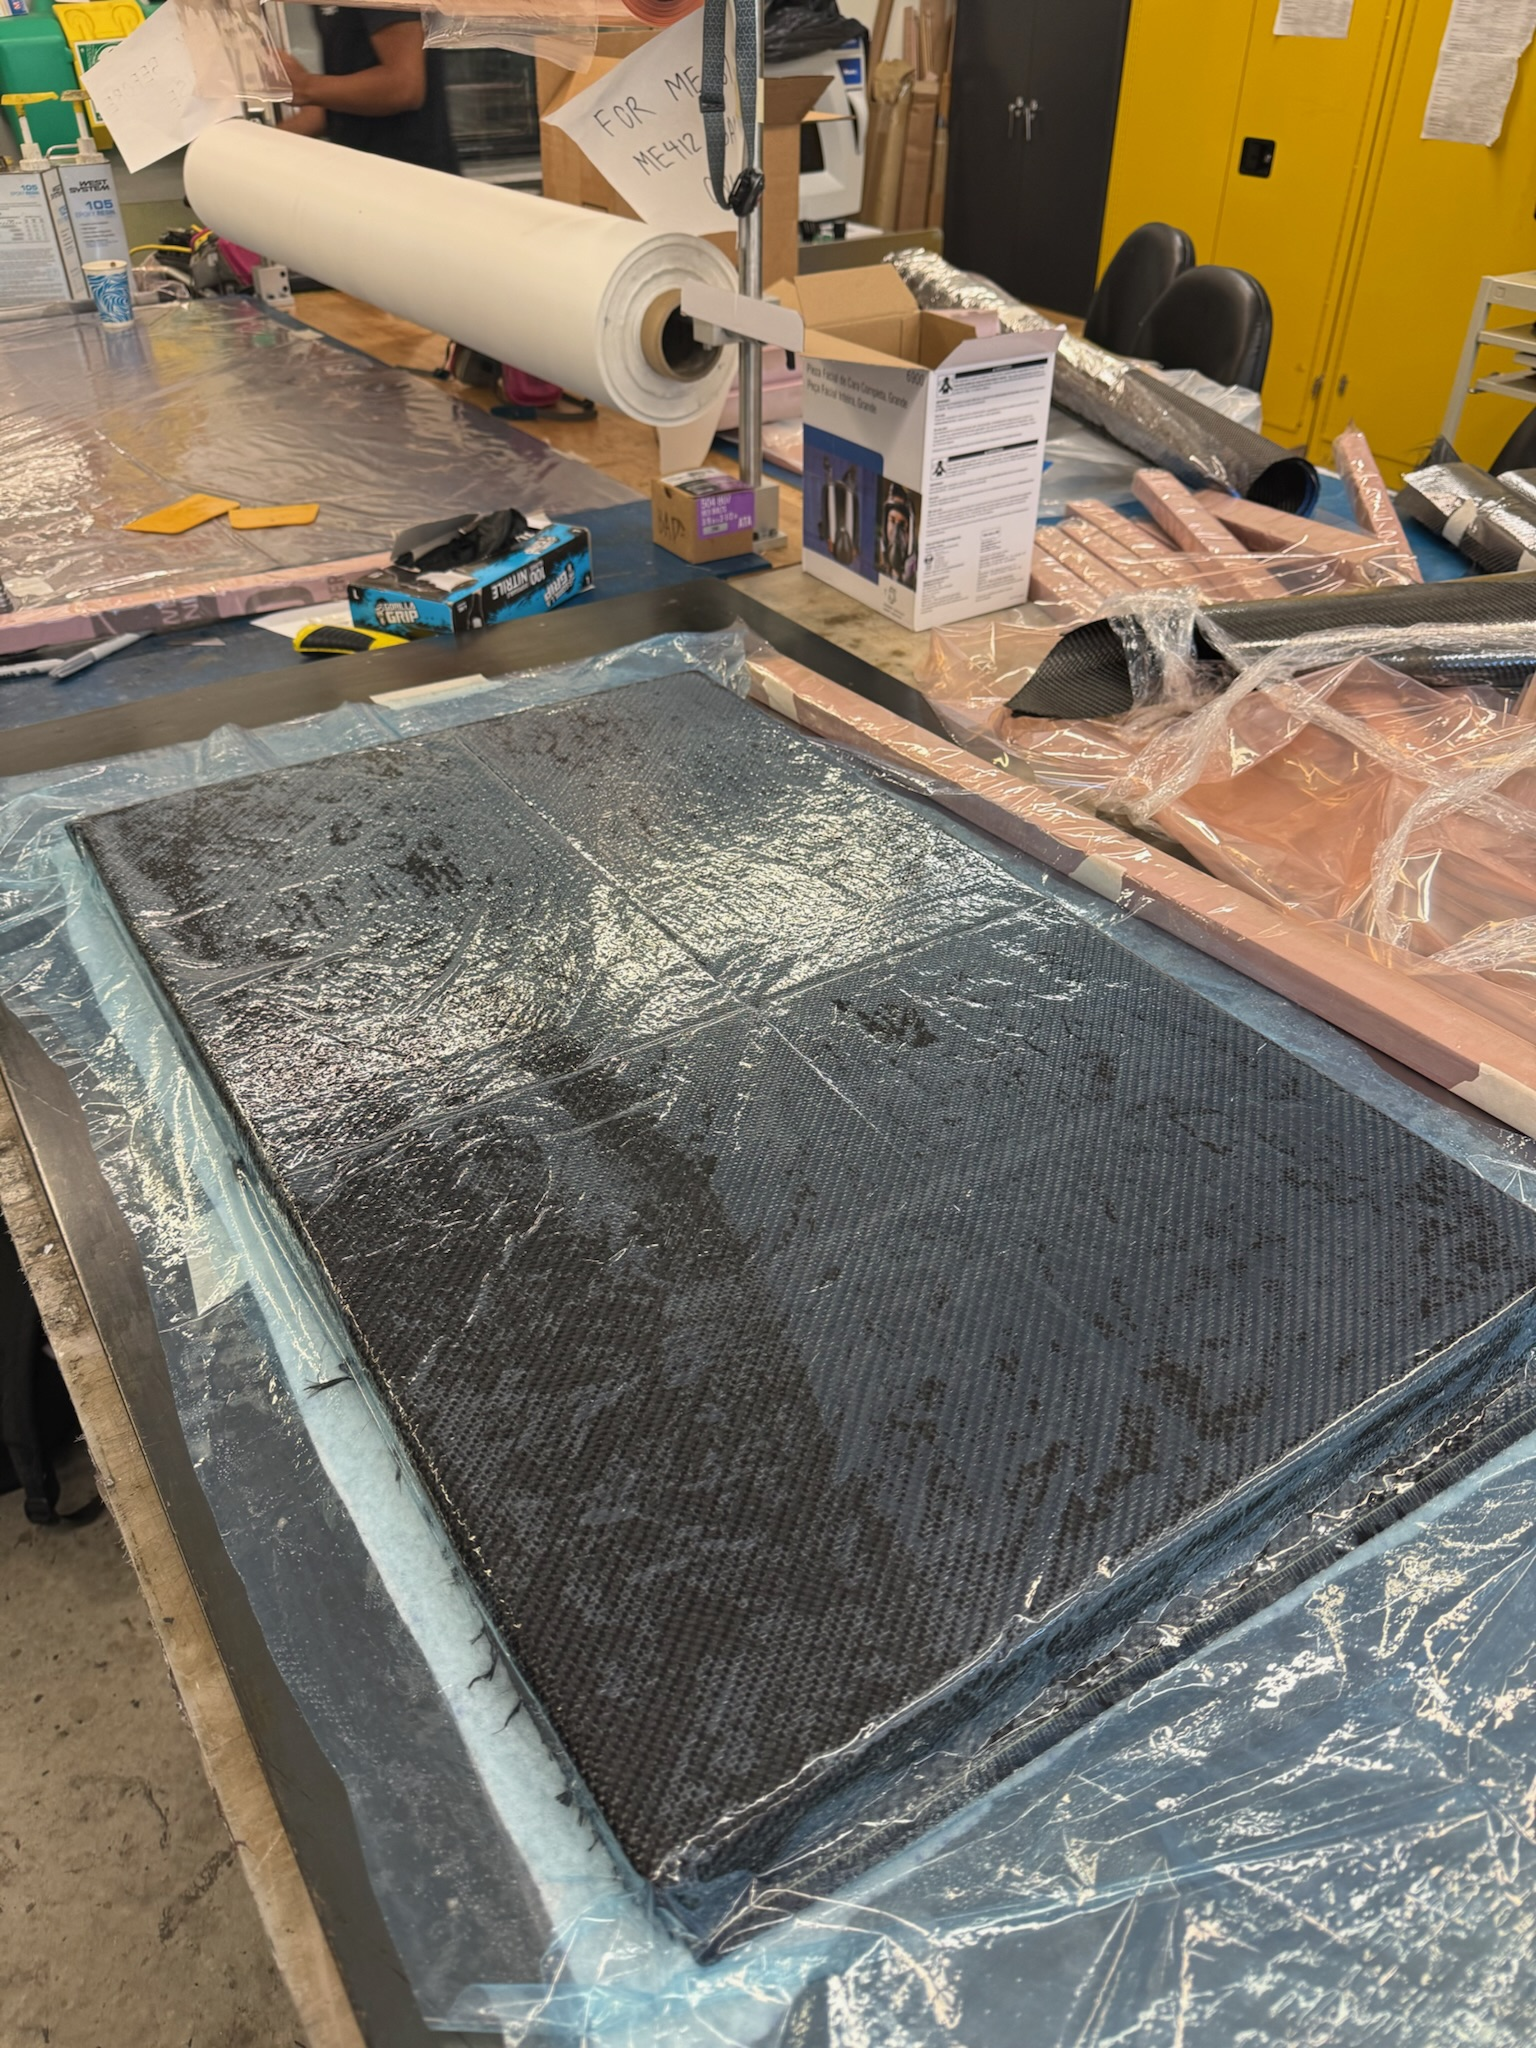
\includegraphics[
        width=3.10in,
        height=1.40in,
        keepaspectratio
    ]{blue_perforrated_film_layup}
};
\draw[RuleGray,line width=0.55pt,rounded corners=4pt]
    ($(current page.north west)+(7.29in,-3.36in)$)
    rectangle
    ($(current page.north east)+(-0.42in,-4.85in)$);

% Row 1 captions
\node[anchor=north,text=Muted,font=\sffamily\fontsize{6.7}{7.3}\selectfont]
at ($(current page.north west)+(2.07in,-4.90in)$)
{1. Waterjet-cut core and perimeter geometry};

\node[anchor=north,text=Muted,font=\sffamily\fontsize{6.7}{7.3}\selectfont]
at ($(current page.north west)+(5.50in,-4.90in)$)
{2. Team wet layup under my process guidance};

\node[anchor=north,text=Muted,font=\sffamily\fontsize{6.7}{7.3}\selectfont]
at ($(current page.north west)+(8.935in,-4.90in)$)
{3. Perforated film, breather, and vacuum enclosure};

% Row 2 image 1
\node[anchor=center,inner sep=0pt]
at ($(current page.north west)+(2.07in,-5.875in)$)
{
    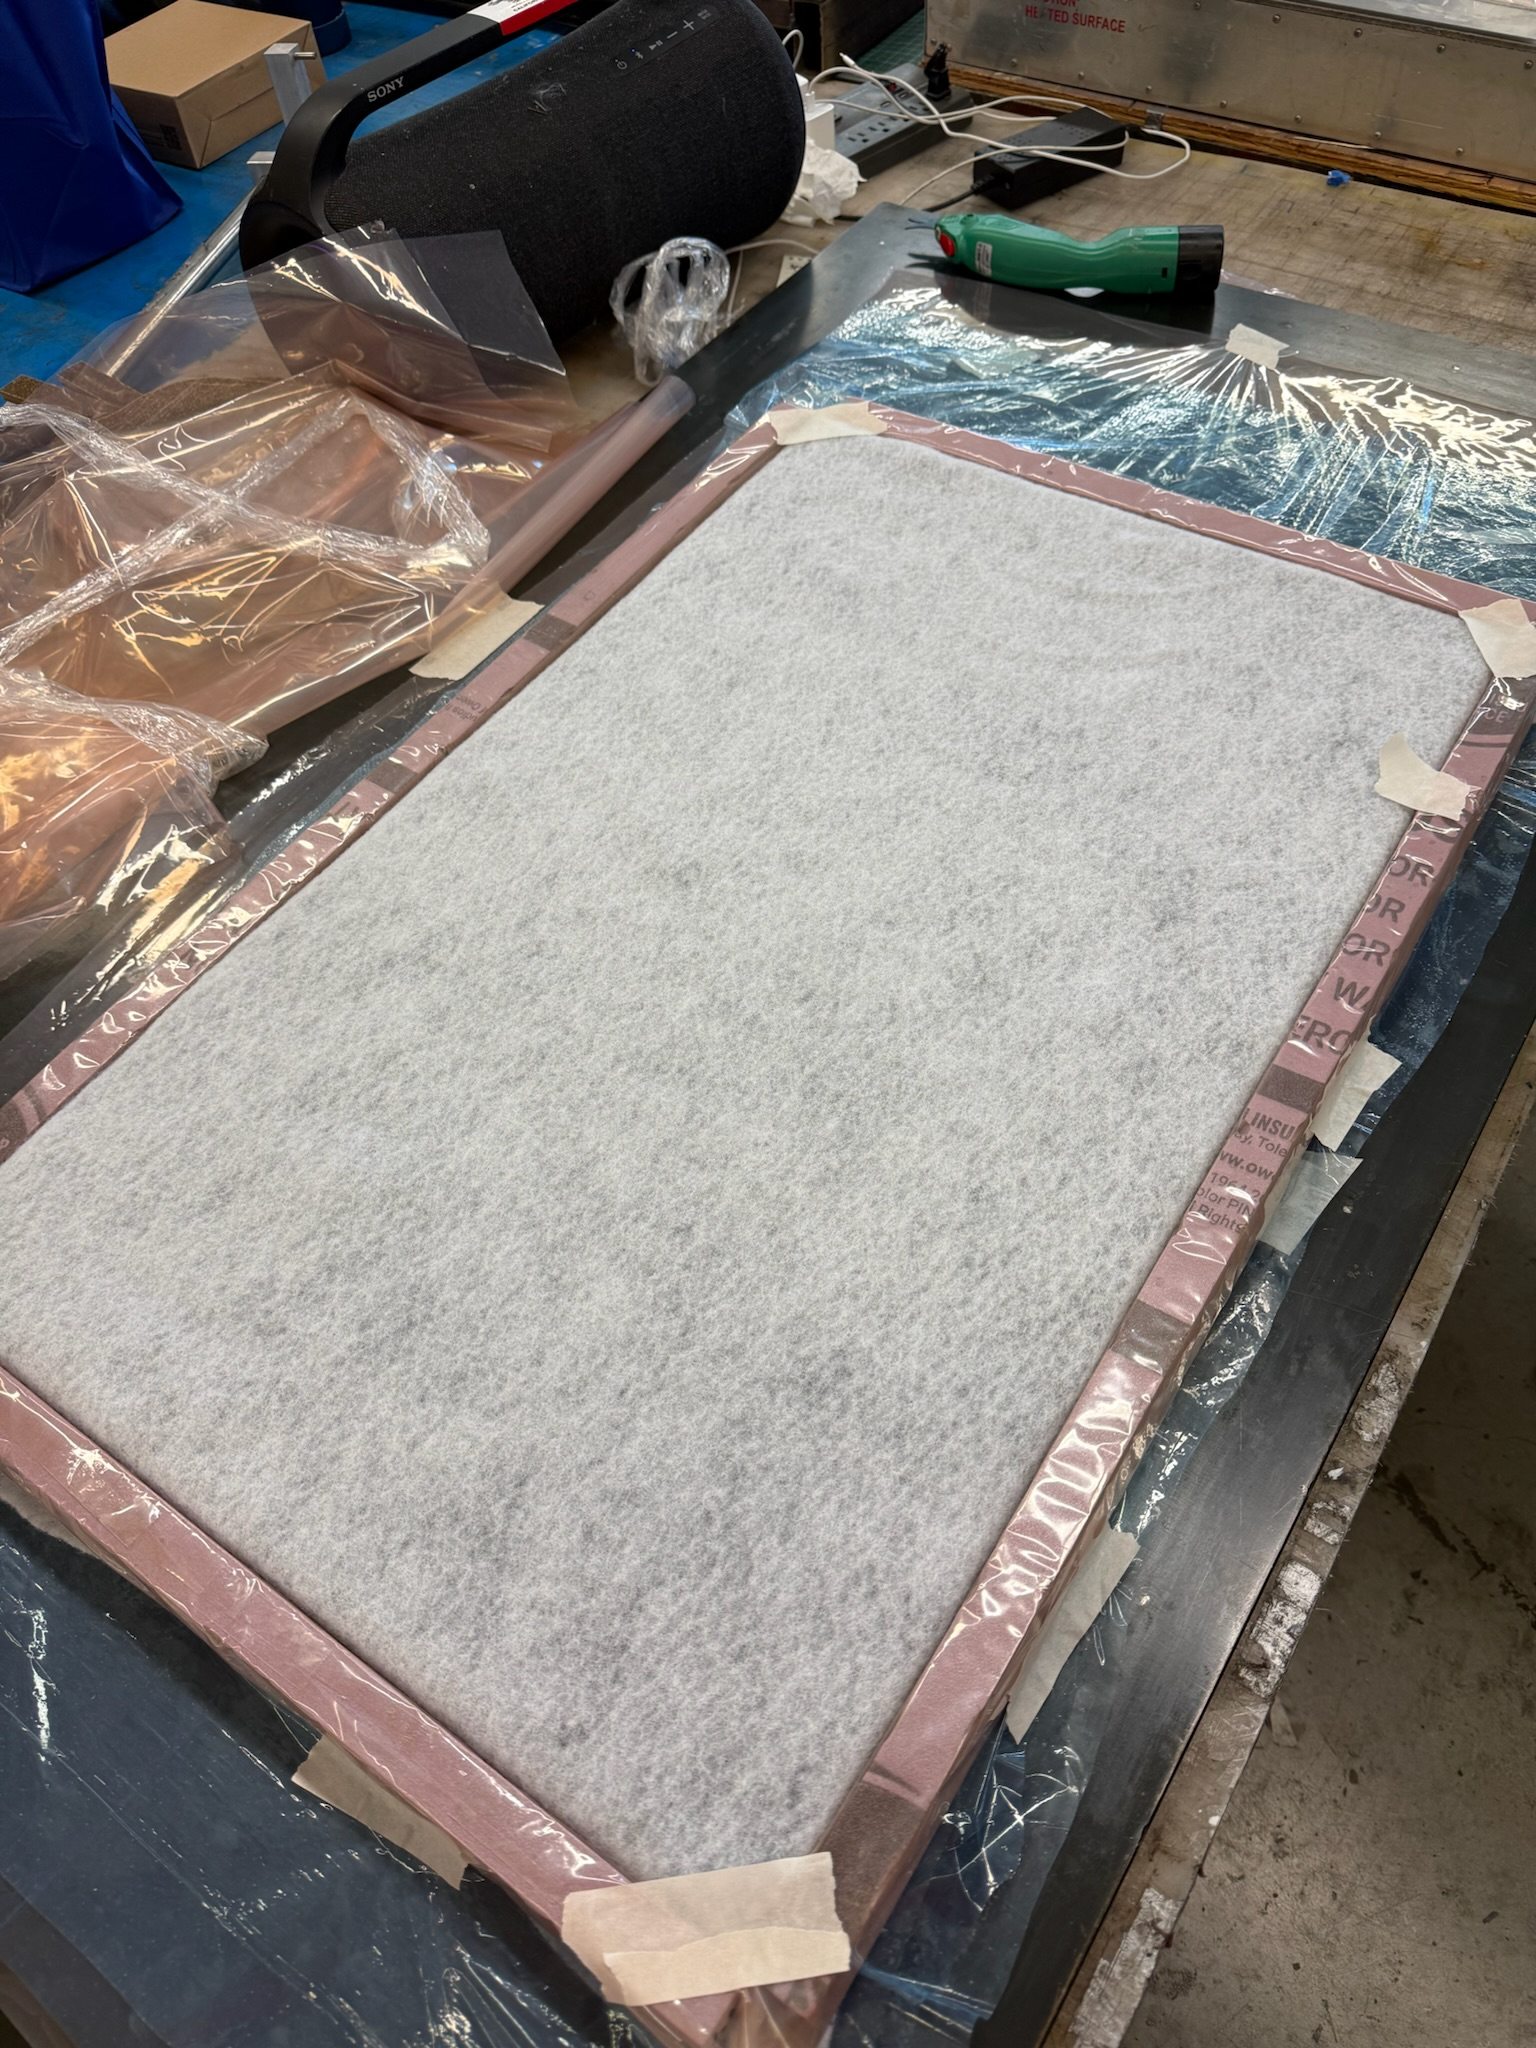
\includegraphics[
        width=3.10in,
        height=1.40in,
        keepaspectratio
    ]{completed_layup}
};
\draw[RuleGray,line width=0.55pt,rounded corners=4pt]
    ($(current page.north west)+(0.43in,-5.13in)$)
    rectangle
    ($(current page.north west)+(3.71in,-6.62in)$);

% Row 2 image 2 — oven chamber used only as a reliable vacuum enclosure; no heat applied
\node[anchor=center,inner sep=0pt]
at ($(current page.north west)+(5.50in,-5.875in)$)
{
    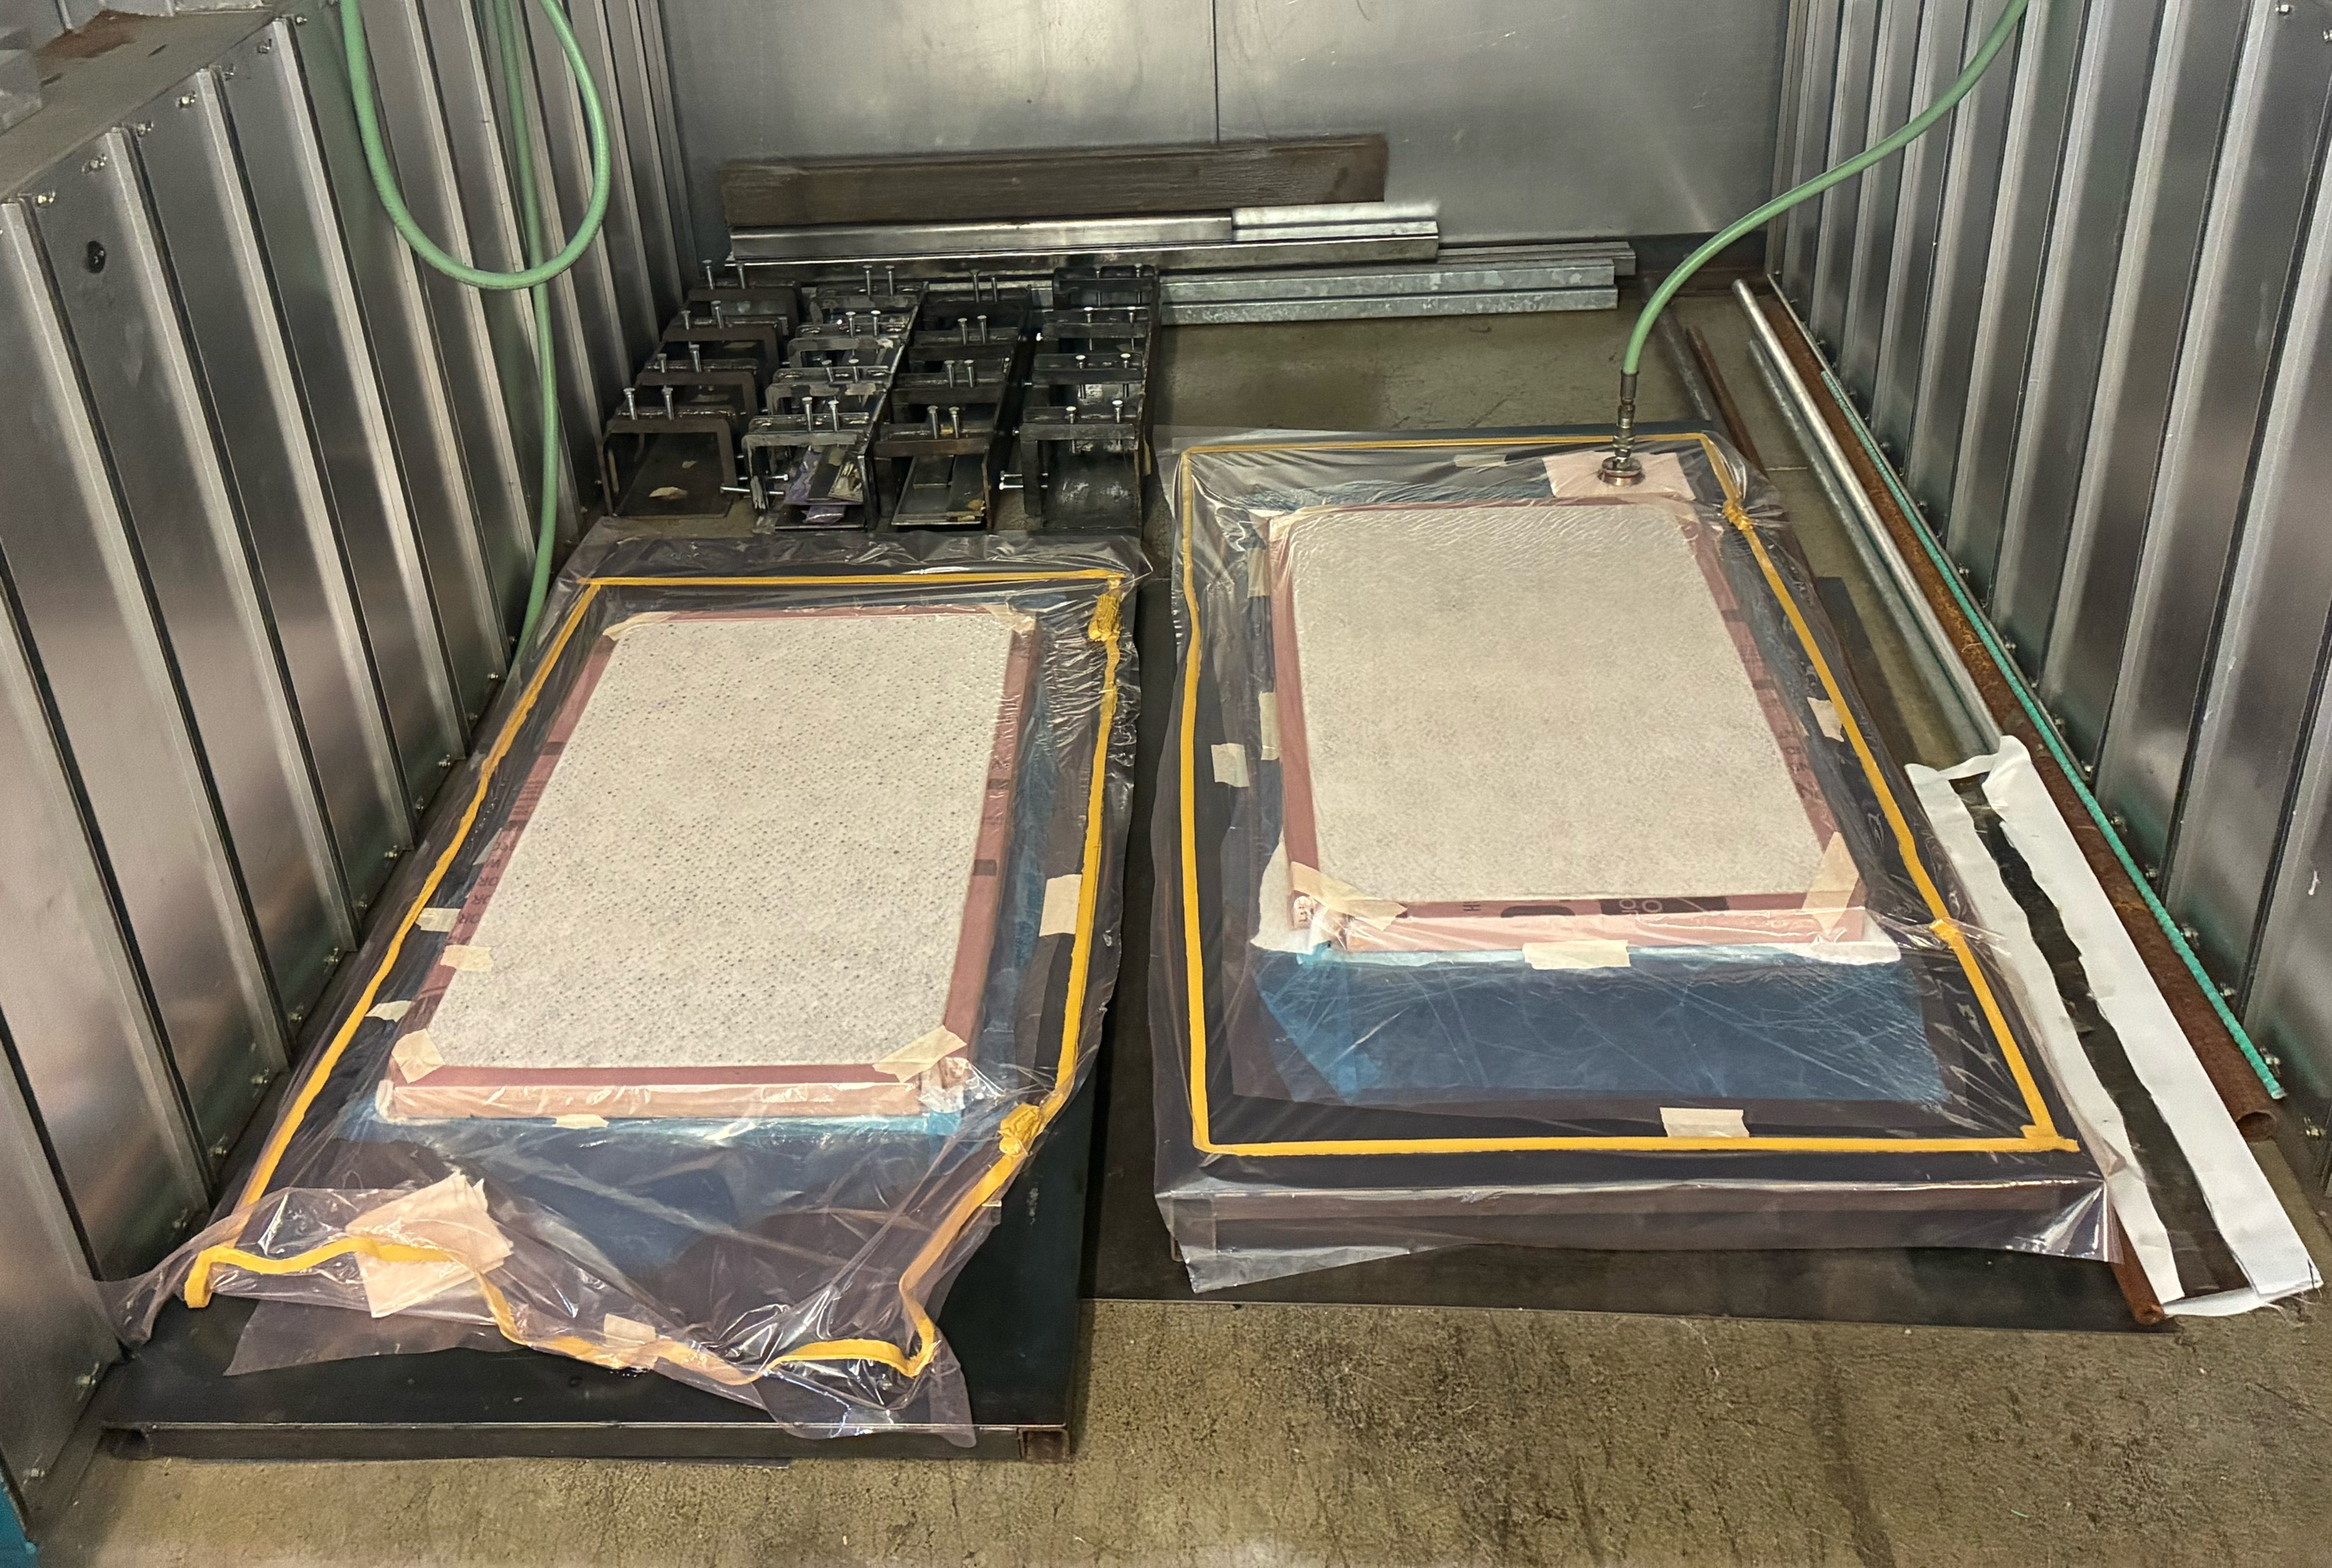
\includegraphics[
        width=3.10in,
        height=1.40in,
        keepaspectratio
    ]{layups_in_composite_oven_under_vacuumPressure}
};
\draw[RuleGray,line width=0.55pt,rounded corners=4pt]
    ($(current page.north west)+(3.86in,-5.13in)$)
    rectangle
    ($(current page.north west)+(7.14in,-6.62in)$);

% Row 2 image 3
\node[anchor=center,inner sep=0pt]
at ($(current page.north west)+(8.935in,-5.875in)$)
{
    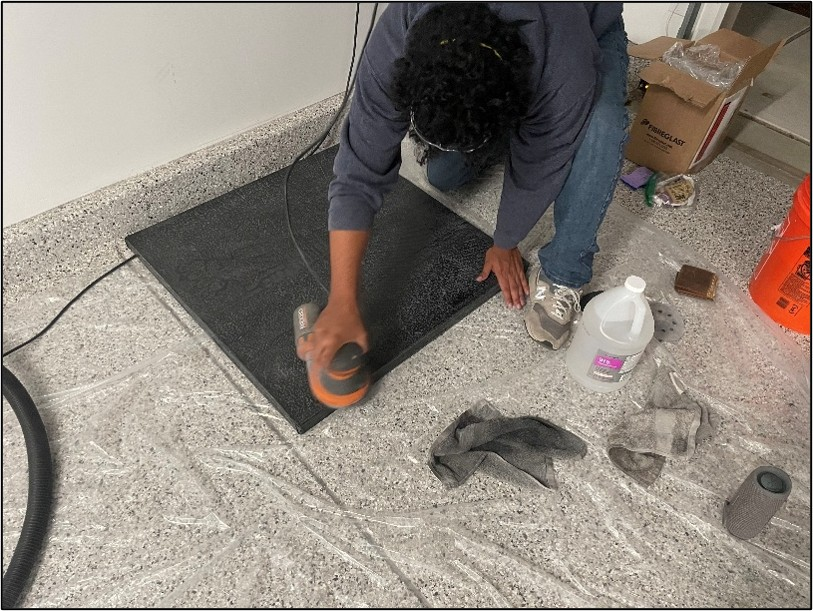
\includegraphics[
        width=3.10in,
        height=1.40in,
        keepaspectratio
    ]{garage_sanding}
};
\draw[RuleGray,line width=0.55pt,rounded corners=4pt]
    ($(current page.north west)+(7.29in,-5.13in)$)
    rectangle
    ($(current page.north east)+(-0.42in,-6.62in)$);

% Row 2 captions
\node[anchor=north,text=Muted,font=\sffamily\fontsize{6.7}{7.3}\selectfont]
at ($(current page.north west)+(2.07in,-6.67in)$)
{4. Fully saturated carbon skin and foam sandwich};

\node[anchor=north,text=Muted,font=\sffamily\fontsize{6.7}{7.3}\selectfont]
at ($(current page.north west)+(5.50in,-6.67in)$)
{5. Room-temperature cure under continuous vacuum};

\node[anchor=north,text=Muted,font=\sffamily\fontsize{6.7}{7.3}\selectfont]
at ($(current page.north west)+(8.935in,-6.67in)$)
{6. Post-processing and surface preparation};

% Bottom callouts
\fill[Panel,rounded corners=4pt]
    ($(current page.north west)+(0.43in,-6.95in)$)
    rectangle
    ($(current page.north west)+(5.48in,-7.60in)$);

\draw[RuleGray,line width=0.55pt,rounded corners=4pt]
    ($(current page.north west)+(0.43in,-6.95in)$)
    rectangle
    ($(current page.north west)+(5.48in,-7.60in)$);

\node[
    anchor=north west,
    text=DeepGreen,
    font=\sffamily\bfseries\fontsize{7.0}{7.6}\selectfont
]
at ($(current page.north west)+(0.63in,-7.08in)$)
{FROM THREE LAYUPS TO ONE};

\node[
    anchor=north west,
    align=left,
    text width=4.56in,
    text=Ink,
    font=\fontsize{6.45}{7.45}\selectfont
]
at ($(current page.north west)+(0.63in,-7.29in)$)
{
The Envelope Method reduced labor, cure cycles, handling,
alignment risk, and time spent forming numerous vacuum-bag
pleats around the 1.5-inch-thick XPS panels.
};

\fill[Panel,rounded corners=4pt]
    ($(current page.north west)+(5.68in,-6.95in)$)
    rectangle
    ($(current page.north east)+(-0.42in,-7.60in)$);

\draw[RuleGray,line width=0.55pt,rounded corners=4pt]
    ($(current page.north west)+(5.68in,-6.95in)$)
    rectangle
    ($(current page.north east)+(-0.42in,-7.60in)$);

\node[
    anchor=north west,
    text=DeepGreen,
    font=\sffamily\bfseries\fontsize{7.0}{7.6}\selectfont
]
at ($(current page.north west)+(5.88in,-7.08in)$)
{WHY SURFACE-BONDED HARDWARE};

\node[
    anchor=north west,
    align=left,
    text width=4.55in,
    text=Ink,
    font=\fontsize{6.45}{7.45}\selectfont
]
at ($(current page.north west)+(5.88in,-7.29in)$)
{
Adhesively bonded hinges and fixtures preserved the clean
composite exterior and avoided drilled inserts, foam-core
crushing, added stress concentrations, and new leak paths.
};


% Footer
\node[
    anchor=south west,
    text=white,
    font=\sffamily\bfseries\fontsize{7.1}{7.7}\selectfont
]
at ($(current page.south west)+(0.42in,0.17in)$)
{\faArrowLeft\ PRODUCT ARCHITECTURE};

\node[
    anchor=south,
    text=white,
    font=\sffamily\fontsize{7.0}{7.6}\selectfont
]
at ($(current page.south)+(0,0.17in)$)
{TORO COVER \hspace{6pt} 2 / 3};

\node[
    anchor=south east,
    text=white,
    font=\sffamily\bfseries\fontsize{7.1}{7.7}\selectfont
]
at ($(current page.south east)+(-0.42in,0.17in)$)
{VALIDATION \& TAKEAWAYS \faArrowRight};

\end{tikzpicture}


% ============================================================
% PAGE 3 — FINISHING, VALIDATION, AND TAKEAWAYS
% ============================================================

\clearpage
\thispagestyle{empty}
\hypertarget{toro-results}{}
\null

\begin{tikzpicture}[remember picture,overlay]

% Background and bars
\fill[white]
    (current page.south west)
    rectangle
    (current page.north east);

\fill[DeepGreen]
    (current page.north west)
    rectangle
    ($(current page.north east)+(0,-0.095in)$);

\fill[PolyGold]
    ($(current page.north west)+(0,-0.095in)$)
    rectangle
    ($(current page.north east)+(0,-0.14in)$);

\fill[DeepGreen]
    (current page.south west)
    rectangle
    ($(current page.south east)+(0,0.36in)$);

\fill[PolyGold]
    ($(current page.south west)+(0,0.36in)$)
    rectangle
    ($(current page.south east)+(0,0.405in)$);

% Header
\node[
    anchor=north west,
    text=PolyGold,
    font=\sffamily\bfseries\fontsize{8.1}{8.7}\selectfont
]
at ($(current page.north west)+(0.42in,-0.39in)$)
{TORO COVER \hspace{5pt}/\hspace{5pt} VALIDATION AND ENGINEERING TAKEAWAYS};

\node[
    anchor=north west,
    text=DeepGreen,
    font=\bfseries\fontsize{22.5}{23.5}\selectfont
]
at ($(current page.north west)+(0.40in,-0.67in)$)
{FROM PROTOTYPE TO PRODUCT PATHWAY};

\node[
    anchor=north west,
    text=Muted,
    font=\sffamily\fontsize{8.7}{9.6}\selectfont
]
at ($(current page.north west)+(0.42in,-1.12in)$)
{Environmental protection, usability testing, scope decisions, and lessons from technical leadership};

\fill[PolyGold]
    ($(current page.north west)+(0.42in,-1.36in)$)
    rectangle
    ($(current page.north west)+(5.8in,-1.315in)$);

% Finishing title
\node[
    anchor=north west,
    text=DeepGreen,
    font=\sffamily\bfseries\fontsize{8.0}{8.7}\selectfont
]
at ($(current page.north west)+(0.43in,-1.62in)$)
{OUTDOOR FINISHING AND ENVIRONMENTAL PROTECTION};

% Image 1
\node[anchor=center,inner sep=0pt]
at ($(current page.north west)+(1.705in,-2.655in)$)
{
    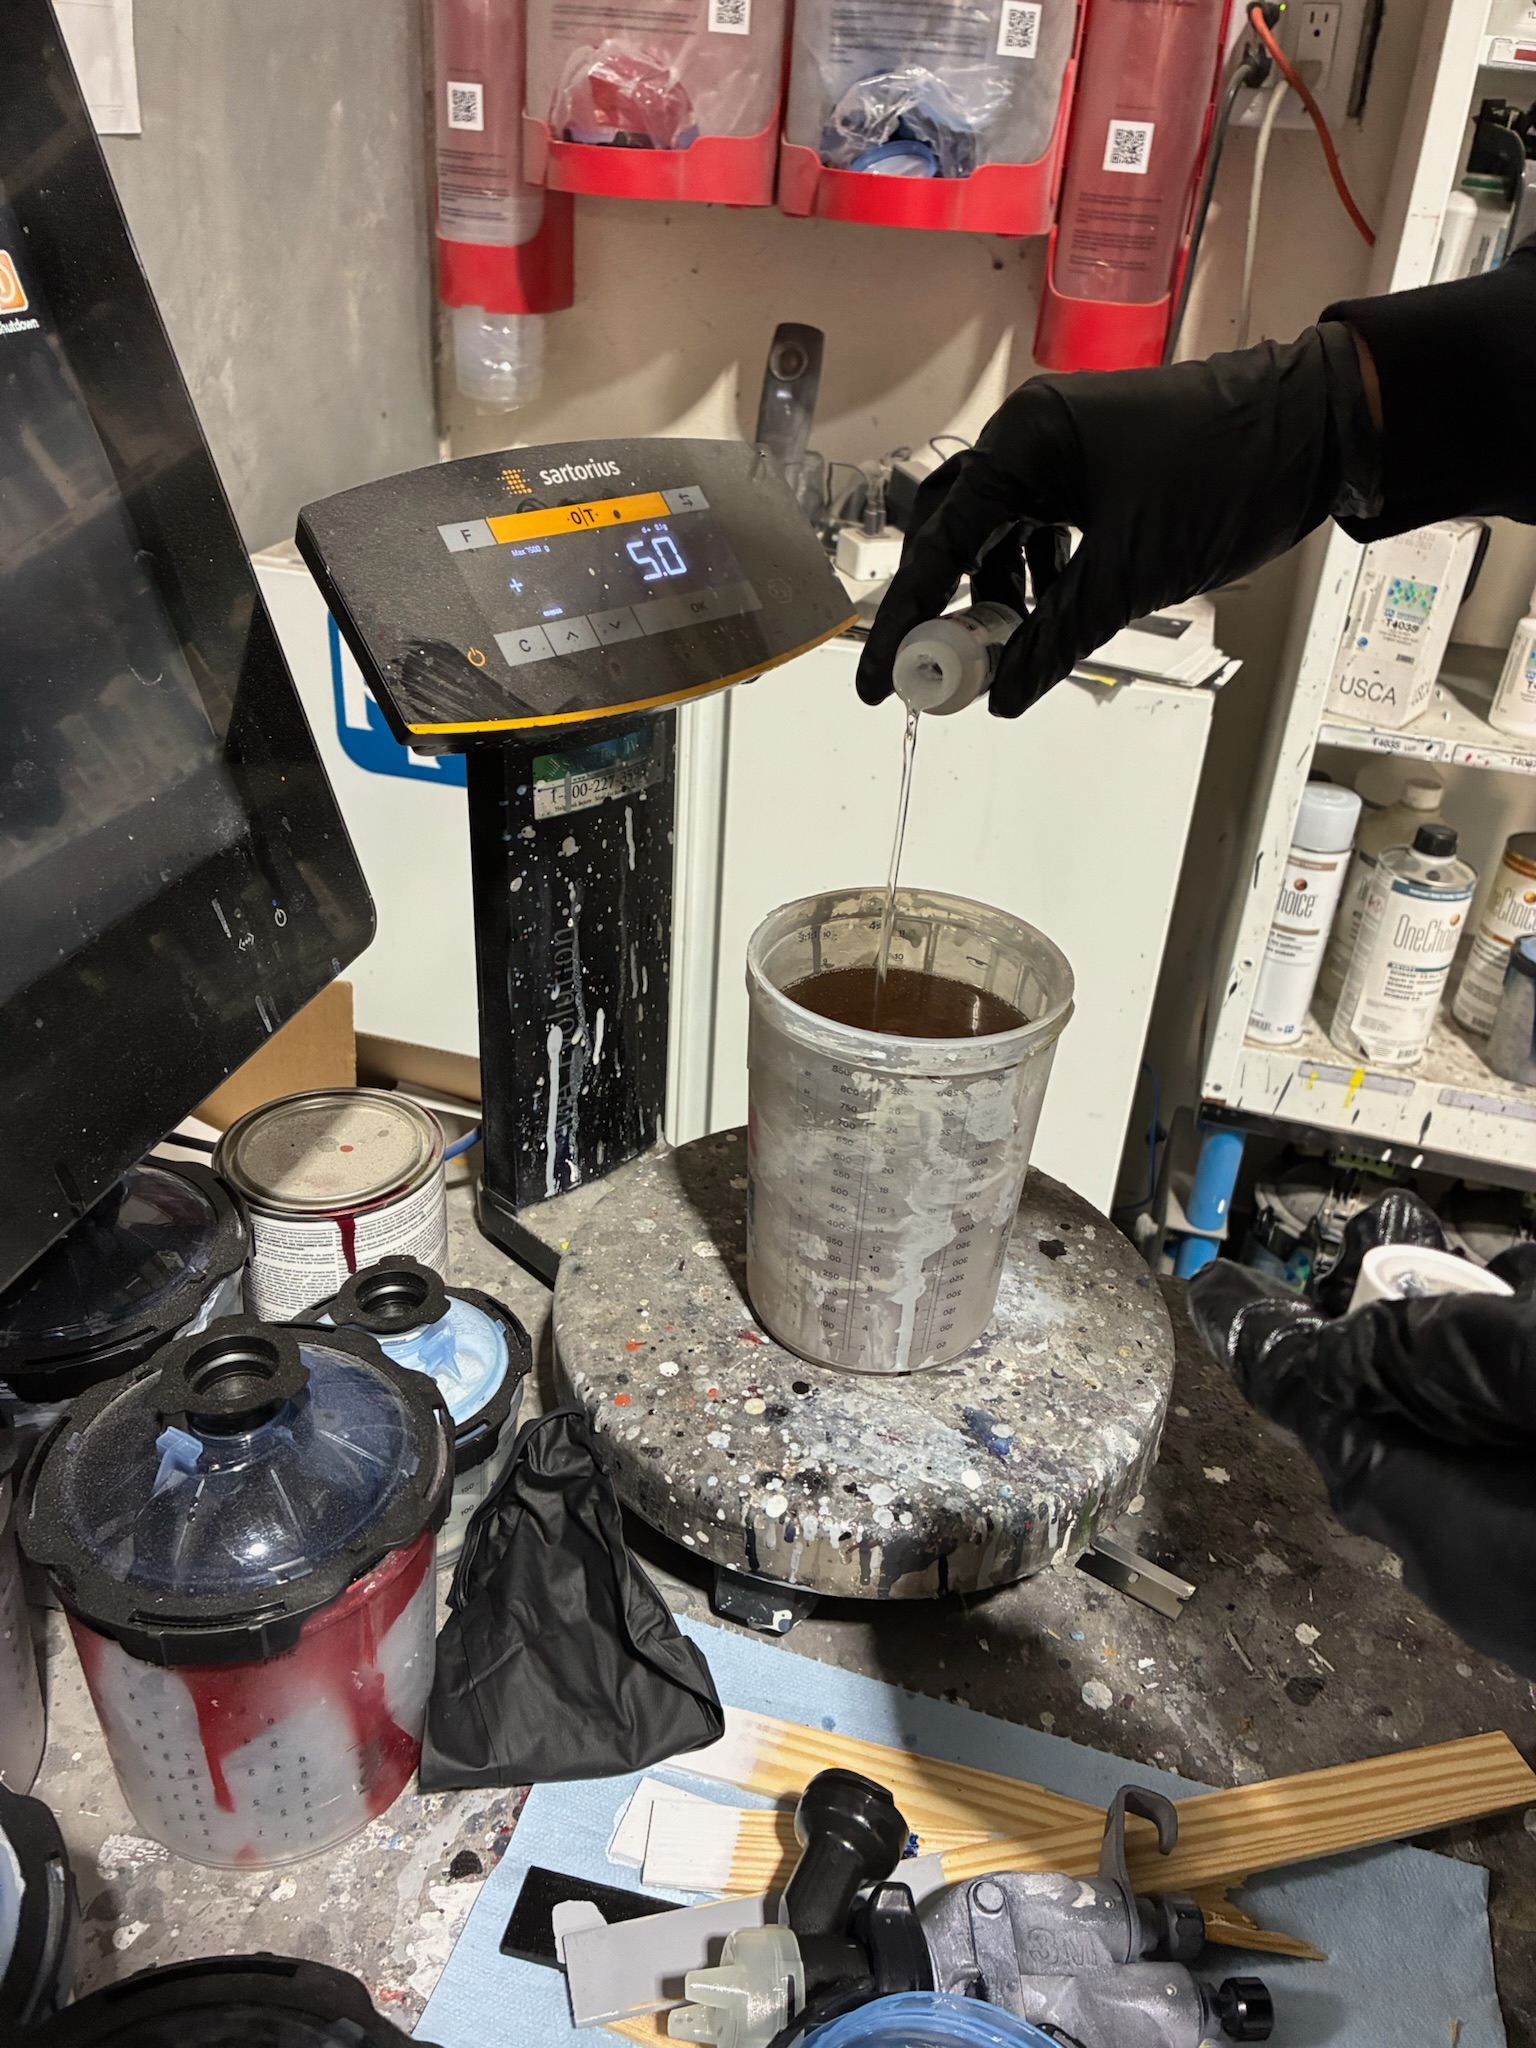
\includegraphics[
        width=2.35in,
        height=1.40in,
        keepaspectratio
    ]{spray_topcoat_prep}
};
\draw[RuleGray,line width=0.55pt,rounded corners=4pt]
    ($(current page.north west)+(0.43in,-1.91in)$)
    rectangle
    ($(current page.north west)+(2.98in,-3.40in)$);

% Image 2
\node[anchor=center,inner sep=0pt]
at ($(current page.north west)+(4.375in,-2.655in)$)
{
    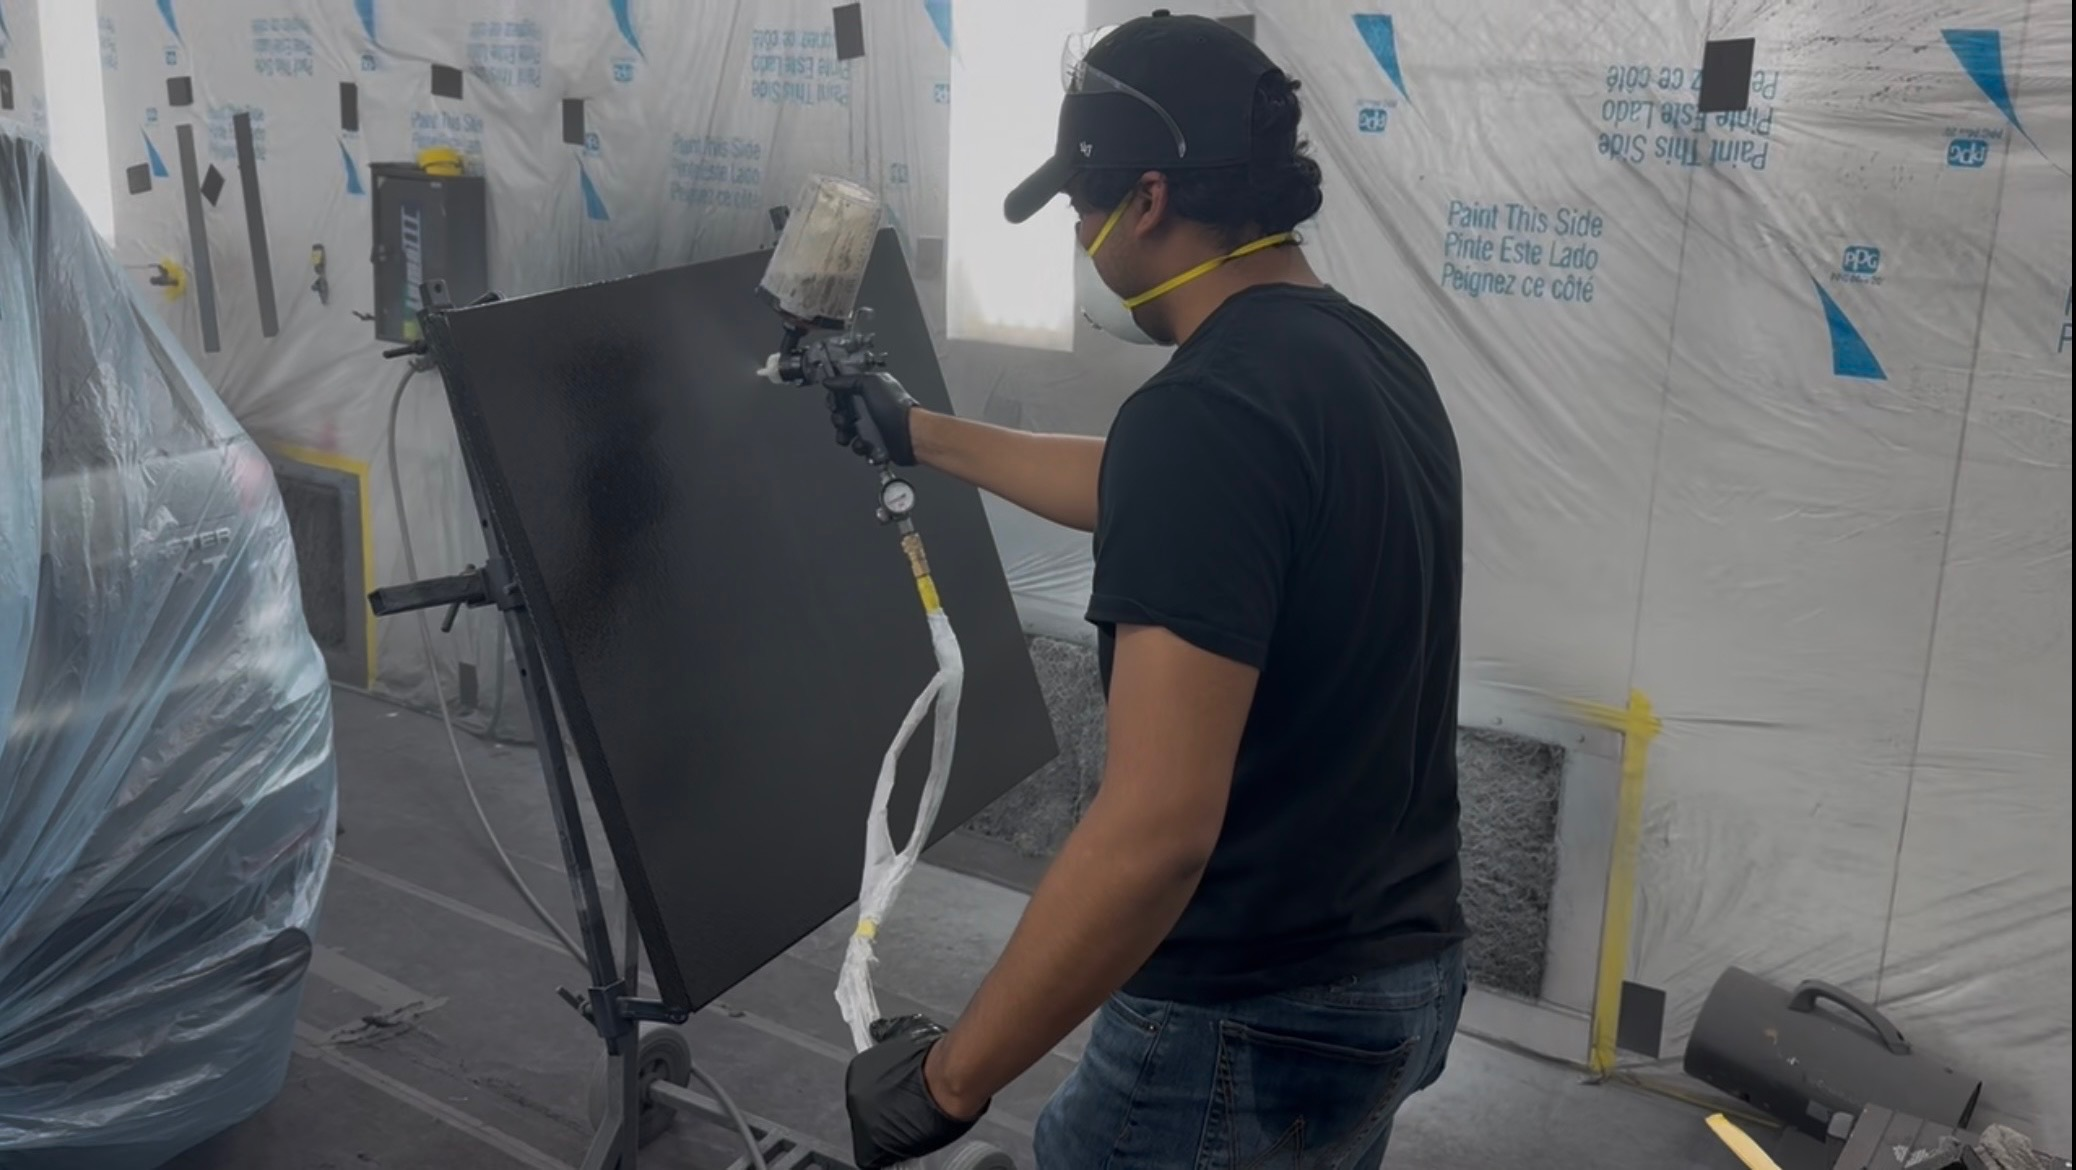
\includegraphics[
        width=2.35in,
        height=1.40in,
        keepaspectratio
    ]{spraying_topcoat}
};
\draw[RuleGray,line width=0.55pt,rounded corners=4pt]
    ($(current page.north west)+(3.10in,-1.91in)$)
    rectangle
    ($(current page.north west)+(5.65in,-3.40in)$);

% Image 3
\node[anchor=center,inner sep=0pt]
at ($(current page.north west)+(7.045in,-2.655in)$)
{
    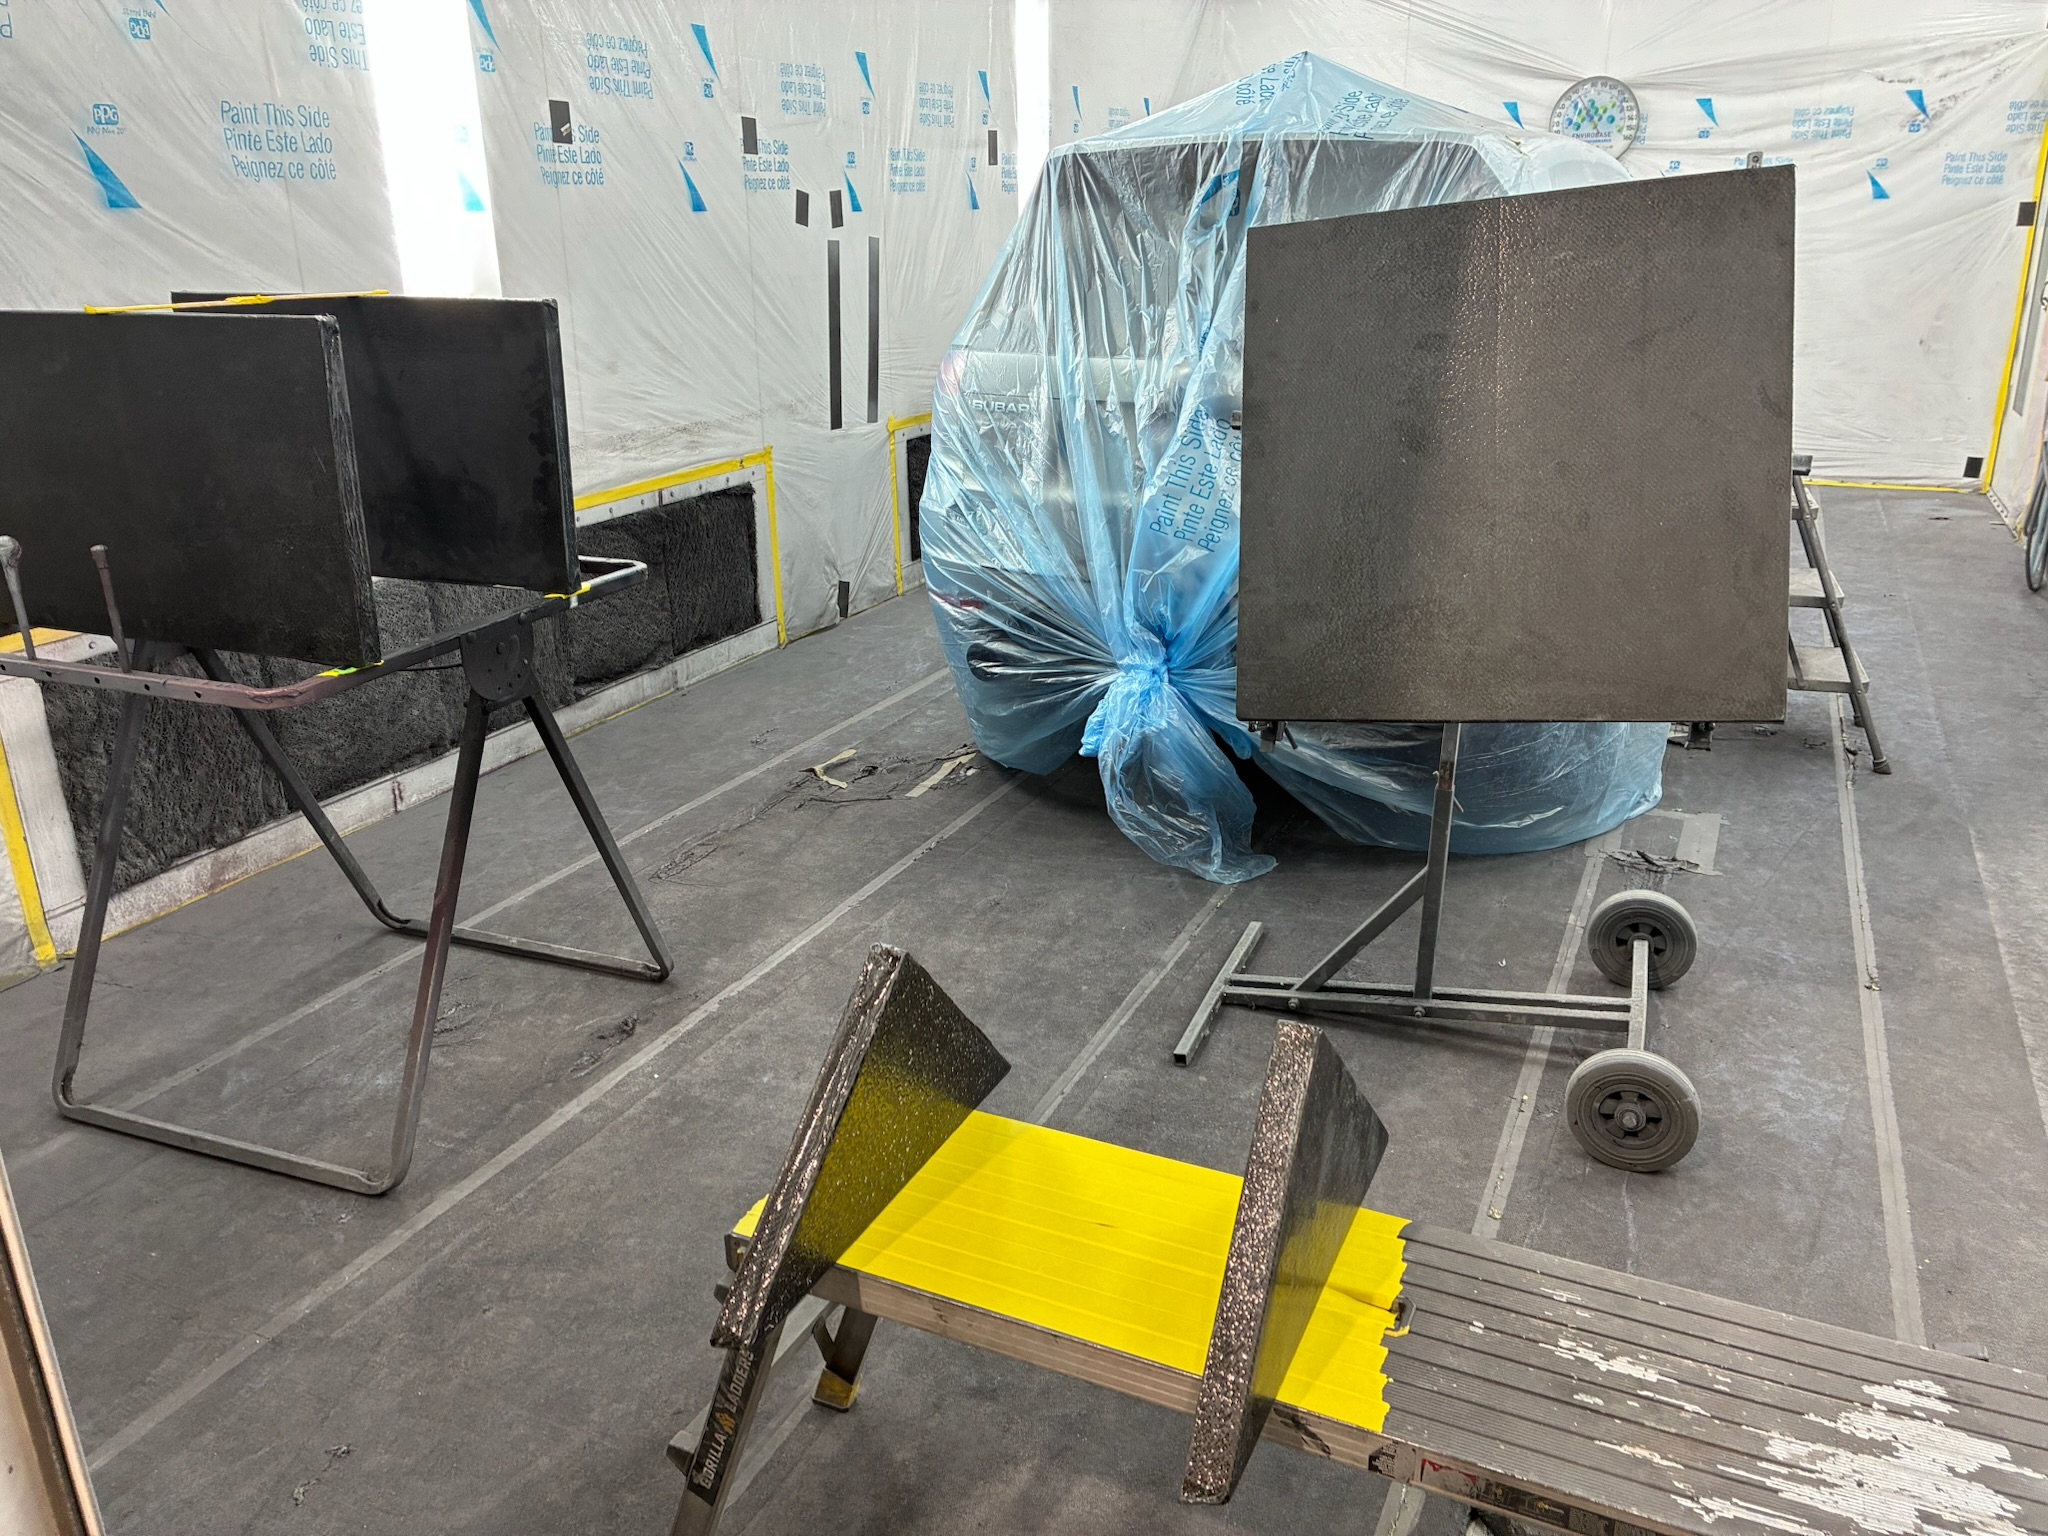
\includegraphics[
        width=2.35in,
        height=1.40in,
        keepaspectratio
    ]{topcoat_setup_apparatus}
};
\draw[RuleGray,line width=0.55pt,rounded corners=4pt]
    ($(current page.north west)+(5.77in,-1.91in)$)
    rectangle
    ($(current page.north west)+(8.32in,-3.40in)$);

% Image 4
\node[anchor=center,inner sep=0pt]
at ($(current page.north west)+(9.50in,-2.655in)$)
{
    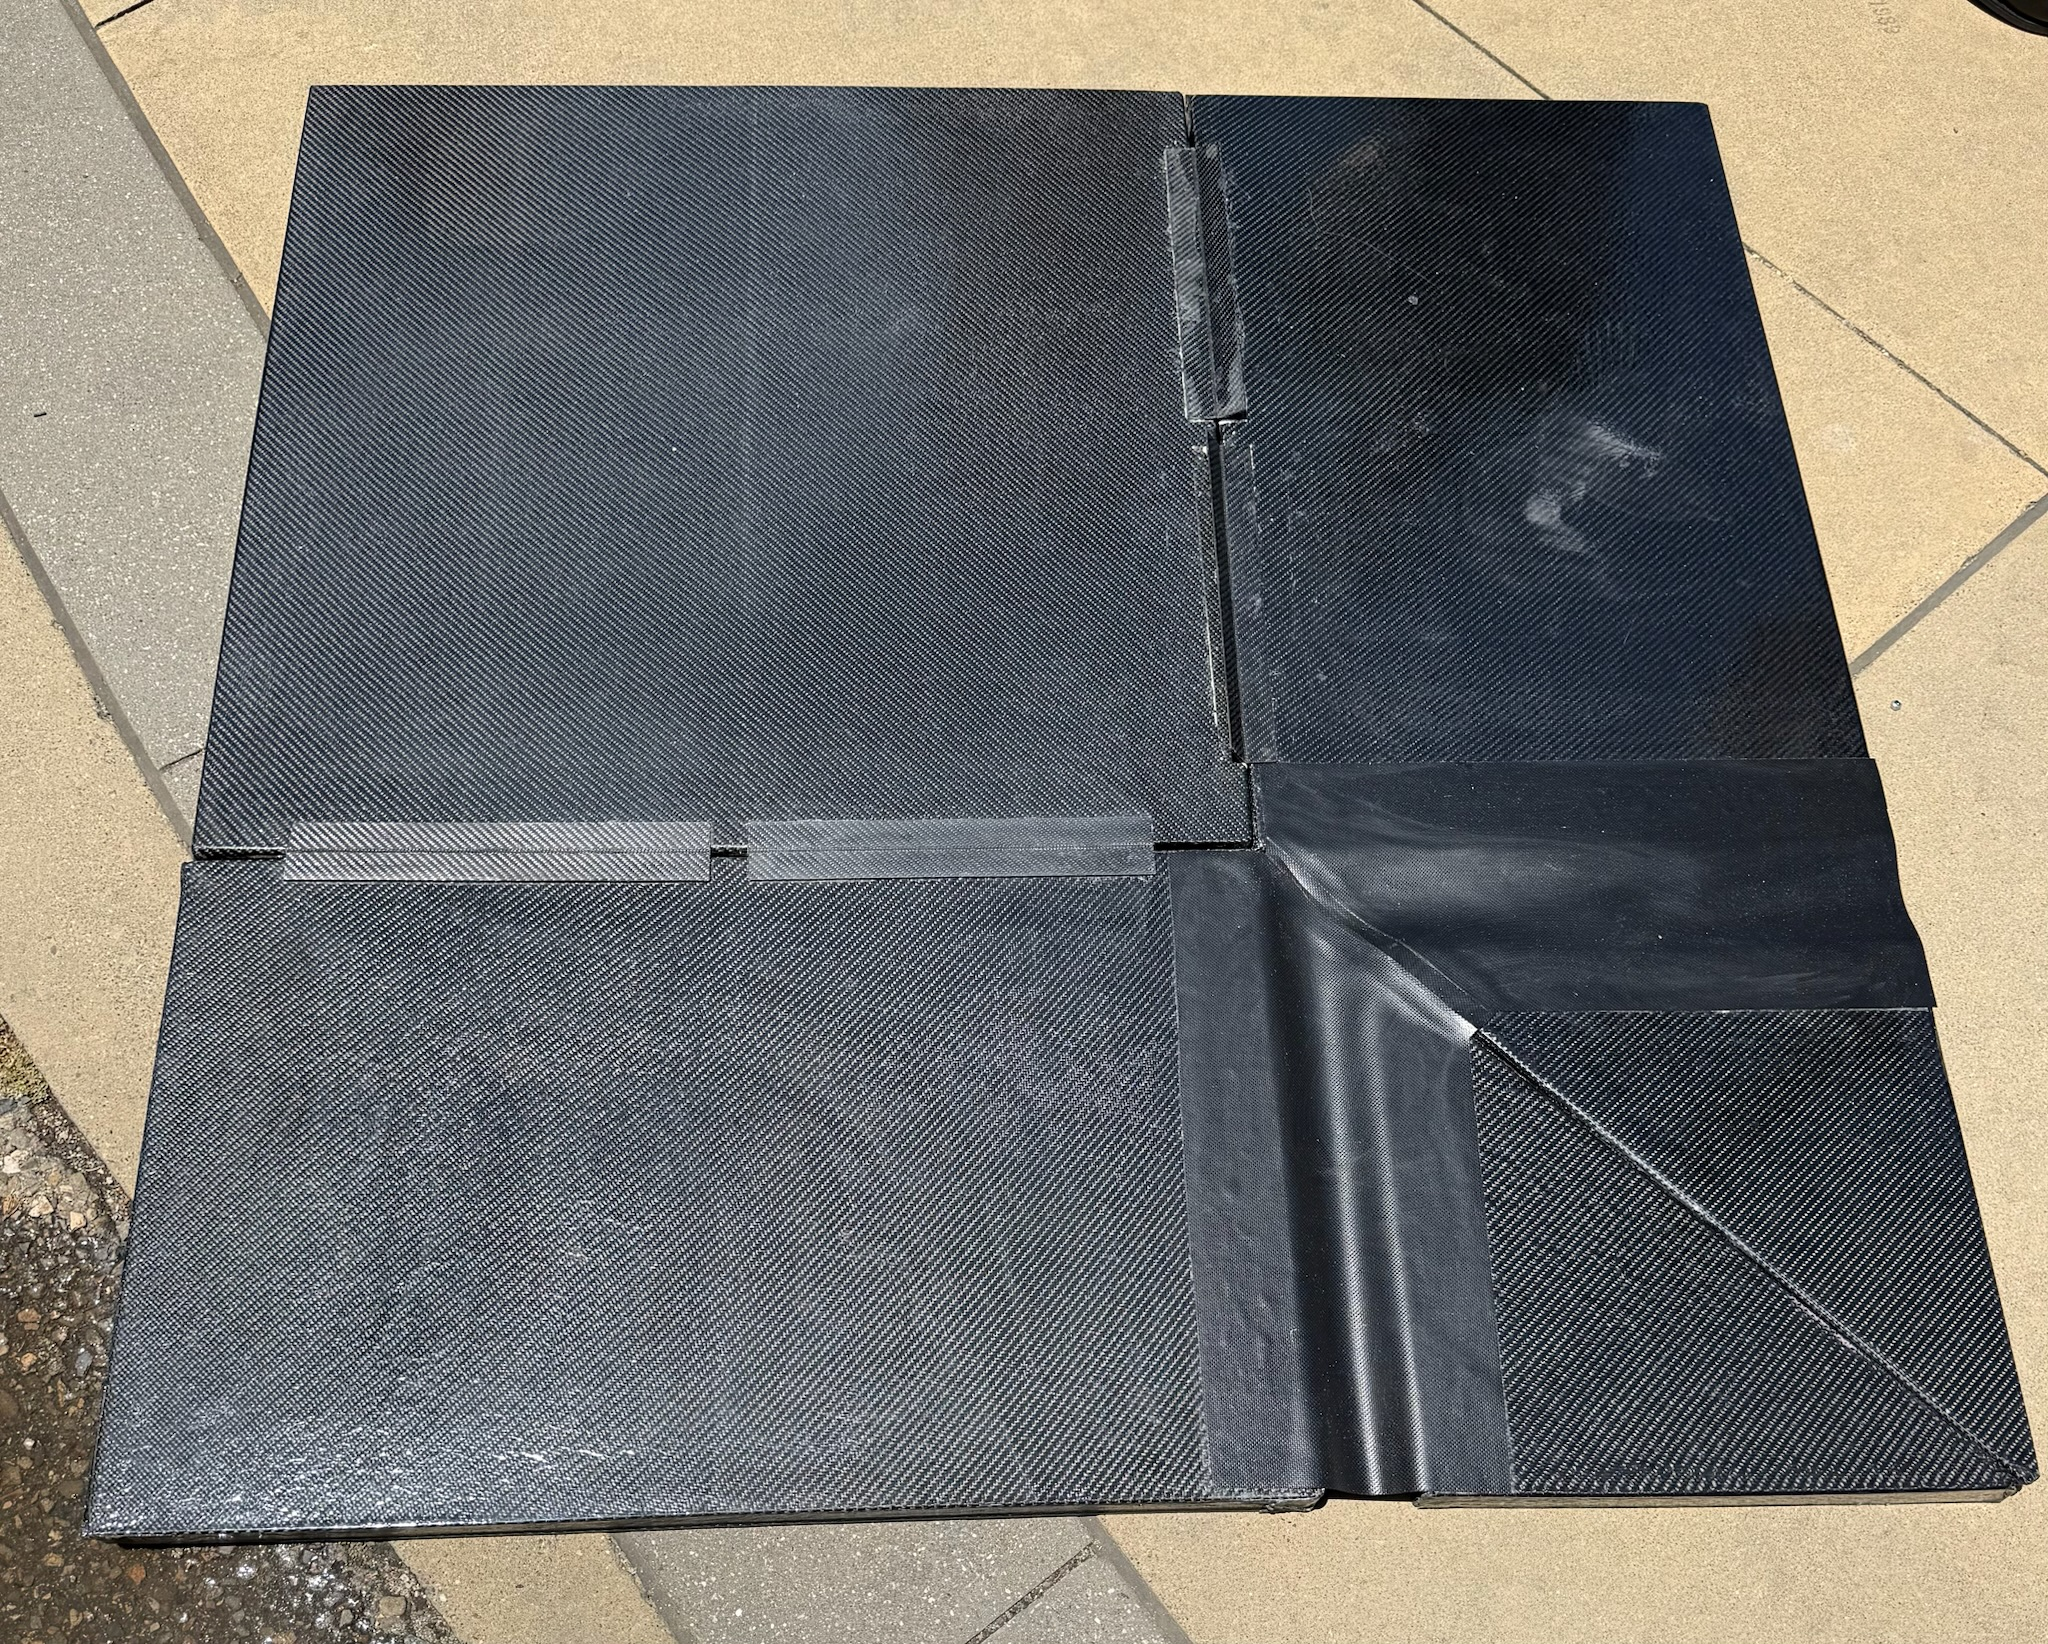
\includegraphics[
        width=2.35in,
        height=1.40in,
        keepaspectratio
    ]{refined_final_toro_cover_partial_carbon_model}
};
\draw[RuleGray,line width=0.55pt,rounded corners=4pt]
    ($(current page.north west)+(8.44in,-1.91in)$)
    rectangle
    ($(current page.north east)+(-0.42in,-3.40in)$);

% Captions
\node[anchor=north,text=Muted,font=\sffamily\fontsize{6.7}{7.3}\selectfont]
at ($(current page.north west)+(1.705in,-3.45in)$)
{Topcoat material preparation};

\node[anchor=north,text=Muted,font=\sffamily\fontsize{6.7}{7.3}\selectfont]
at ($(current page.north west)+(4.375in,-3.45in)$)
{Automotive-booth topcoat application};

\node[anchor=north,text=Muted,font=\sffamily\fontsize{6.7}{7.3}\selectfont]
at ($(current page.north west)+(7.045in,-3.45in)$)
{Coated panels drying after application};

\node[anchor=north,text=Muted,font=\sffamily\fontsize{6.7}{7.3}\selectfont]
at ($(current page.north west)+(9.50in,-3.45in)$)
{Partial carbon manufacturing model};

% Environmental rationale
\fill[SoftGold,rounded corners=4pt]
    ($(current page.north west)+(0.43in,-3.73in)$)
    rectangle
    ($(current page.north east)+(-0.42in,-4.76in)$);

\node[
    anchor=north west,
    align=left,
    text width=9.75in,
    text=Ink,
    font=\fontsize{7.05}{8.25}\selectfont
]
at ($(current page.north west)+(0.65in,-3.89in)$)
{
Because the sponsor required a carbon-fiber cover for outdoor use near chlorinated water,
environmental protection became a functional requirement rather than a cosmetic finish.
I selected and personally sprayed a UV-resistant Sunshield topcoat to seal minor laminate
porosity, reduce moisture ingress, preserve the carbon appearance, limit UV degradation of
the epoxy matrix, and isolate the composite surface from nearby metallic hardware.
};

% Results title
\node[
    anchor=north west,
    text=DeepGreen,
    font=\sffamily\bfseries\fontsize{8.0}{8.7}\selectfont
]
at ($(current page.north west)+(0.43in,-4.94in)$)
{FUNCTIONAL PROTOTYPE RESULTS};

% ------------------------------------------------------------
% Matched lower panels — larger type and improved allocation
% ------------------------------------------------------------

% Left results panel
\fill[SoftGreen,rounded corners=5pt]
    ($(current page.north west)+(0.43in,-5.22in)$)
    rectangle
    ($(current page.north west)+(5.98in,-7.39in)$);

\draw[RuleGray,line width=0.65pt,rounded corners=5pt]
    ($(current page.north west)+(0.43in,-5.22in)$)
    rectangle
    ($(current page.north west)+(5.98in,-7.39in)$);

\fill[DeepGreen,rounded corners=5pt]
    ($(current page.north west)+(0.43in,-5.22in)$)
    rectangle
    ($(current page.north west)+(5.98in,-5.58in)$);

\fill[DeepGreen]
    ($(current page.north west)+(0.43in,-5.40in)$)
    rectangle
    ($(current page.north west)+(5.98in,-5.58in)$);

\node[anchor=west,text=white,
      font=\sffamily\bfseries\fontsize{7.0}{7.6}\selectfont]
at ($(current page.north west)+(0.66in,-5.40in)$)
{SPECIFICATION};

\node[anchor=west,text=white,
      font=\sffamily\bfseries\fontsize{7.0}{7.6}\selectfont]
at ($(current page.north west)+(3.02in,-5.40in)$)
{RESULT};

\node[anchor=east,text=white,
      font=\sffamily\bfseries\fontsize{7.0}{7.6}\selectfont]
at ($(current page.north west)+(5.55in,-5.40in)$)
{STATUS};

\node[
    anchor=north west,
    align=left,
    text width=2.15in,
    text=Ink,
    font=\bfseries\fontsize{7.15}{8.55}\selectfont
]
at ($(current page.north west)+(0.66in,-5.72in)$)
{
Deployment time\\[3.4pt]
Removal time\\[3.4pt]
Single-user operation\\[3.4pt]
Single-side operation\\[3.4pt]
Deployment steps\\[3.4pt]
Removal steps\\[3.4pt]
Weight\\[3.4pt]
Folded storage
};

\node[
    anchor=north west,
    align=left,
    text width=1.45in,
    text=Ink,
    font=\fontsize{7.15}{8.55}\selectfont
]
at ($(current page.north west)+(3.02in,-5.72in)$)
{
25.51 seconds\\[3.4pt]
37.22 seconds\\[3.4pt]
100\% successful\\[3.4pt]
75\% successful\\[3.4pt]
6.4 average\\[3.4pt]
9 average\\[3.4pt]
17 lb\\[3.4pt]
2.9' x 2.9' x 1.7'
};

\node[
    anchor=north east,
    align=right,
    text width=1.05in,
    text=DeepGreen,
    font=\sffamily\bfseries\fontsize{7.05}{8.55}\selectfont
]
at ($(current page.north west)+(5.55in,-5.72in)$)
{
PASS\\[3.4pt]
PASS\\[3.4pt]
PASS\\[3.4pt]
NEAR TARGET\\[3.4pt]
PASS\\[3.4pt]
PASS\\[3.4pt]
NEAR TARGET\\[3.4pt]
PASS
};

% Right takeaways panel — widened for easier reading
\fill[SoftGreen,rounded corners=5pt]
    ($(current page.north west)+(6.14in,-5.22in)$)
    rectangle
    ($(current page.north east)+(-0.42in,-7.39in)$);

\draw[RuleGray,line width=0.65pt,rounded corners=5pt]
    ($(current page.north west)+(6.14in,-5.22in)$)
    rectangle
    ($(current page.north east)+(-0.42in,-7.39in)$);

\fill[DeepGreen,rounded corners=5pt]
    ($(current page.north west)+(6.14in,-5.22in)$)
    rectangle
    ($(current page.north east)+(-0.42in,-5.58in)$);

\fill[DeepGreen]
    ($(current page.north west)+(6.14in,-5.40in)$)
    rectangle
    ($(current page.north east)+(-0.42in,-5.58in)$);

\node[anchor=west,text=white,
      font=\sffamily\bfseries\fontsize{7.1}{7.7}\selectfont]
at ($(current page.north west)+(6.38in,-5.40in)$)
{ENGINEERING TAKEAWAYS};

\node[
    anchor=north west,
    align=left,
    text width=4.02in,
    text=Ink,
    font=\fontsize{6.75}{7.85}\selectfont
]
at ($(current page.north west)+(6.38in,-5.72in)$)
{
\textbf{Manufacturing first.}
Composite manufacturing constraints should guide the product architecture from the beginning.\\[4.5pt]
\textbf{Prioritize deliberately.}
Competing requirements must be balanced intentionally instead of maximizing every objective.\\[4.5pt]
\textbf{Lead through the process.}
Clear procedures, calm communication, and respect for teammates' strengths were essential during fabrication.\\[4.5pt]
\textbf{Next iteration.}
Reduce weight, refine the fabric-hinge fold lines, and improve panel-edge clearance.
};

% Compact concluding pathway
\node[
    anchor=center,
    align=center,
    text=PolyGold,
    font=\sffamily\bfseries\fontsize{6.3}{6.9}\selectfont
]
at ($(current page.north)+(3.06in,-7.18in)$)
{PROTOTYPE \faArrowRight\ DESIGN REFINEMENT
\faArrowRight\ REPEATABLE MANUFACTURING
\faArrowRight\ PRODUCT};

% Validation resources
\node[
    anchor=north,
    align=center,
    text=DeepGreen,
    font=\sffamily\bfseries\fontsize{6.6}{7.2}\selectfont
]
at ($(current page.north)+(0,-7.58in)$)
{\href{\ToroDeploymentLink}{\faPlayCircle\ DEPLOYMENT}
\hspace{18pt}
\href{\ToroRemovalLink}{\faPlayCircle\ REMOVAL / FOLDING}
\hspace{18pt}
\href{\ToroPosterLink}{\faFilePdf\ EXPO POSTER}
\hspace{18pt}
\href{\ToroReportLink}{\faFilePdf\ FINAL REPORT}};

% Footer
\node[
    anchor=south west,
    text=white,
    font=\sffamily\bfseries\fontsize{7.1}{7.7}\selectfont
]
at ($(current page.south west)+(0.42in,0.17in)$)
{\faArrowLeft\ MANUFACTURING-DRIVEN DESIGN};

\node[
    anchor=south,
    text=white,
    font=\sffamily\fontsize{7.0}{7.6}\selectfont
]
at ($(current page.south)+(0,0.17in)$)
{TORO COVER \hspace{6pt} 3 / 3};

\node[
    anchor=south east,
    text=white,
    font=\sffamily\bfseries\fontsize{7.1}{7.7}\selectfont
]
at ($(current page.south east)+(-0.42in,0.17in)$)
{NEXT PROJECT \faArrowRight};

\end{tikzpicture}
\input{paddle}
\clearpage
 before \end{document}.
% 3. Image references use the original Overleaf base filenames
%    without extensions.
% ============================================================



% ============================================================
% CLICKABLE PROJECT RESOURCES
% All links use the exact Google Drive resources supplied.
% ============================================================
\providecommand{\ToroDrawingLink}{https://drive.google.com/file/d/1A7-7wMnRNLuQDaTgxeuUCBsGNqyXzOGV/view?usp=sharing}
\providecommand{\ToroDimensionsLink}{https://drive.google.com/file/d/13sw3BNJvE8GdzlRffxoF2n5r9Gzxide7/view?usp=sharing}
\providecommand{\ToroProblemLink}{https://drive.google.com/file/d/1zHtl8zrb13F1yeN74ptawpfS5UM_xsuw/view?usp=drive_link}
\providecommand{\ToroReportLink}{https://drive.google.com/file/d/1ULZ-P46lFsC2x29ZfmRVIKgYnr9o8hMt/view?usp=drive_link}
\providecommand{\ToroPosterLink}{https://drive.google.com/file/d/1vKiKaJUcHQb_db-FkZnRF6EvtuM4hKyS/view?usp=drive_link}
\providecommand{\ToroDeploymentLink}{https://drive.google.com/file/d/1XJx34o80_mZPTl7xy93HtWAgtS3ThhvY/view?usp=drive_link}
\providecommand{\ToroRemovalLink}{https://drive.google.com/file/d/1O7xYeyB67NUwT-j1B1HeiCcHnZDYjk6_/view?usp=drive_link}

% ============================================================
% PAGE 1 — PROJECT OVERVIEW, OWNERSHIP, AND ARCHITECTURE
% ============================================================

\clearpage
\thispagestyle{empty}
\hypertarget{toro}{}
\null

\begin{tikzpicture}[remember picture,overlay]

% Background
\fill[white]
    (current page.south west)
    rectangle
    (current page.north east);

% Page bars
\fill[DeepGreen]
    (current page.north west)
    rectangle
    ($(current page.north east)+(0,-0.095in)$);

\fill[PolyGold]
    ($(current page.north west)+(0,-0.095in)$)
    rectangle
    ($(current page.north east)+(0,-0.14in)$);

\fill[DeepGreen]
    (current page.south west)
    rectangle
    ($(current page.south east)+(0,0.36in)$);

\fill[PolyGold]
    ($(current page.south west)+(0,0.36in)$)
    rectangle
    ($(current page.south east)+(0,0.405in)$);

% Header
\node[
    anchor=north west,
    text=PolyGold,
    font=\sffamily\bfseries\fontsize{8.1}{8.7}\selectfont
]
at ($(current page.north west)+(0.42in,-0.39in)$)
{01 COMPOSITES \hspace{5pt}/\hspace{5pt} PROJECT 01};

\node[
    anchor=north west,
    text=DeepGreen,
    font=\bfseries\fontsize{23.5}{24.5}\selectfont
]
at ($(current page.north west)+(0.40in,-0.67in)$)
{TORO CARBON FIBER SAFETY COVER};

\node[
    anchor=north west,
    text=Muted,
    font=\sffamily\fontsize{8.4}{9.2}\selectfont
]
at ($(current page.north west)+(0.42in,-1.12in)$)
{Cal Poly Composites Laboratory \hspace{7pt}\textbullet\hspace{7pt}
Team Project \hspace{7pt}\textbullet\hspace{7pt}
Fall--Spring 2026 \hspace{7pt}\textbullet\hspace{7pt}
San Luis Obispo, California};

\fill[PolyGold]
    ($(current page.north west)+(0.42in,-1.37in)$)
    rectangle
    ($(current page.north west)+(6.1in,-1.325in)$);

% Challenge text
\node[
    anchor=north west,
    text=DeepGreen,
    font=\sffamily\bfseries\fontsize{8.1}{8.8}\selectfont
]
at ($(current page.north west)+(0.43in,-1.61in)$)
{THE CHALLENGE};

\node[
    anchor=north west,
    align=left,
    text width=4.47in,
    text=Ink,
    font=\fontsize{8.05}{9.65}\selectfont
]
at ($(current page.north west)+(0.43in,-1.84in)$)
{
Develop a lightweight cover for a 6 ft by 6 ft in-ground spa
that could be deployed by one person, stored compactly,
provide insulation, resist a poolside environment, and maintain
a refined appearance. The sponsor supplied an ambitious but
intentionally broad project statement, requiring the team to
define the product architecture, priorities, manufacturing
strategy, and realistic path toward future commercialization.
};

% Role box
\fill[SoftGold,rounded corners=5pt]
    ($(current page.north west)+(0.42in,-2.88in)$)
    rectangle
    ($(current page.north west)+(4.98in,-4.58in)$);

\fill[PolyGold]
    ($(current page.north west)+(0.42in,-2.88in)$)
    rectangle
    ($(current page.north west)+(0.52in,-4.58in)$);

\node[
    anchor=north west,
    text=DeepGreen,
    font=\sffamily\bfseries\fontsize{8.1}{8.8}\selectfont
]
at ($(current page.north west)+(0.66in,-3.02in)$)
{MY ROLE — DESIGN \& MANUFACTURING LEAD};

\node[
    anchor=north west,
    align=left,
    text width=4.02in,
    text=Ink,
    font=\fontsize{7.05}{8.15}\selectfont
]
at ($(current page.north west)+(0.66in,-3.27in)$)
{
\textbullet\ Modeled every custom part and the complete assembly\\[1.5pt]
\textbullet\ Produced the engineering drawing package independently\\[1.5pt]
\textbullet\ Developed the composite-panel manufacturing process\\[1.5pt]
\textbullet\ Created all waterjet DXFs and manufacturing geometry\\[1.5pt]
\textbullet\ Trained teammates in wet layup and vacuum bagging\\[1.5pt]
\textbullet\ Presented feasibility, scope, and tradeoffs to the sponsor
};

% Large deployed foam-model image
\node[anchor=center,inner sep=0pt]
at ($(current page.north west)+(8.00in,-3.04in)$)
{
    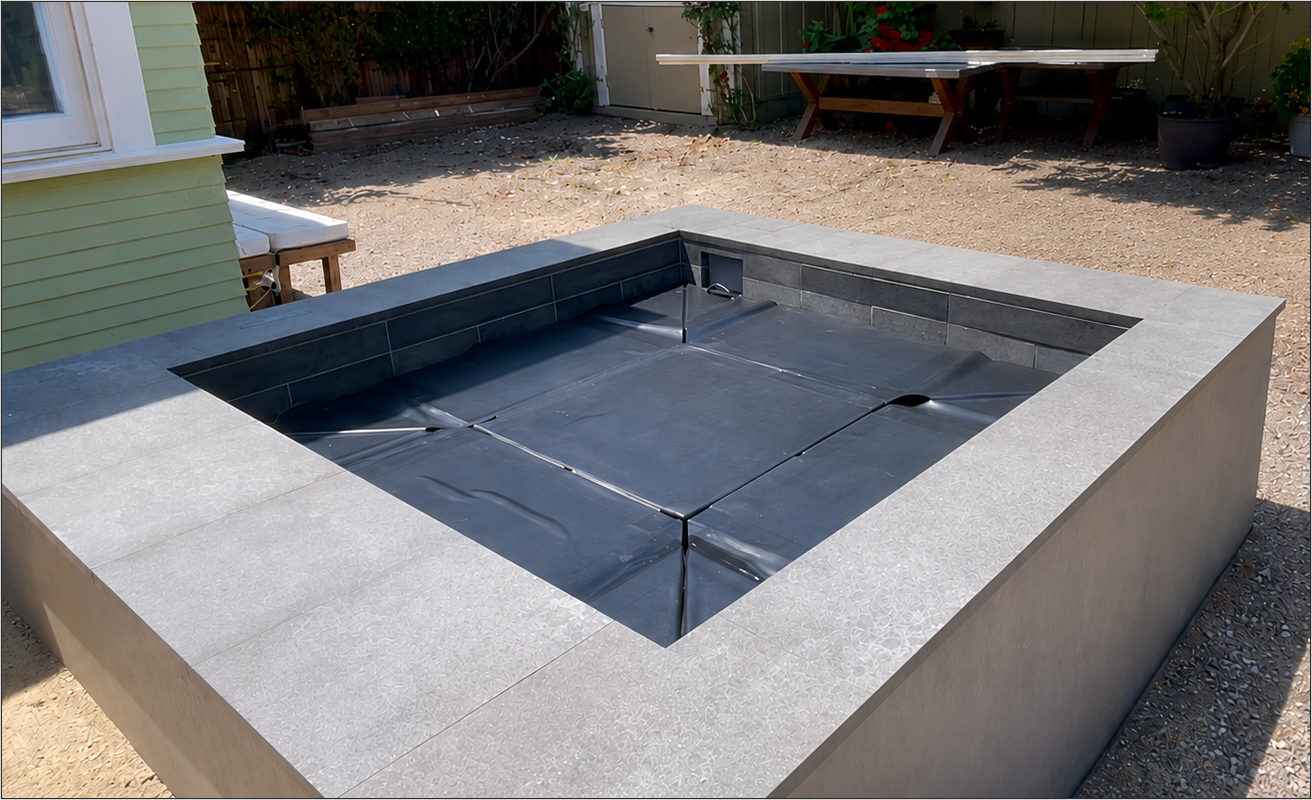
\includegraphics[
        width=5.55in,
        height=2.78in,
        keepaspectratio
    ]{deployed_functional_prototype}
};

\draw[DeepGreen,line width=0.8pt,rounded corners=7pt]
    ($(current page.north west)+(5.16in,-1.61in)$)
    rectangle
    ($(current page.north east)+(-0.42in,-4.47in)$);

\node[
    anchor=north west,
    text=Muted,
    font=\sffamily\fontsize{6.2}{6.9}\selectfont
]
at ($(current page.north west)+(5.18in,-4.54in)$)
{Functional foam model deployed over the sponsor's in-ground spa.};

% Image-strip title
\node[
    anchor=north west,
    text=DeepGreen,
    font=\sffamily\bfseries\fontsize{8.1}{8.8}\selectfont
]
at ($(current page.north west)+(0.43in,-4.78in)$)
{PRODUCT DEVELOPMENT AND FINAL ARCHITECTURE};

% Five-image development strip — CAD-first sequence
% Image 1: topside CAD
\node[anchor=center,inner sep=0pt]
at ($(current page.north west)+(1.47in,-5.73in)$)
{
    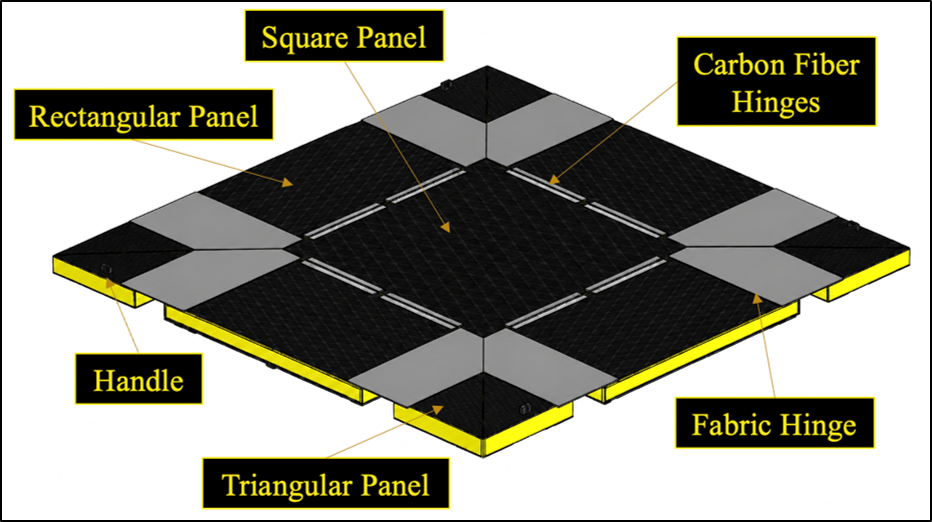
\includegraphics[
        width=1.92in,
        height=1.30in,
        keepaspectratio
    ]{Toro_Cover_topside_Cad}
};
\draw[RuleGray,line width=0.55pt,rounded corners=4pt]
    ($(current page.north west)+(0.43in,-5.04in)$)
    rectangle
    ($(current page.north west)+(2.51in,-6.43in)$);

% Image 2: underside CAD
\node[anchor=center,inner sep=0pt]
at ($(current page.north west)+(3.66in,-5.73in)$)
{
    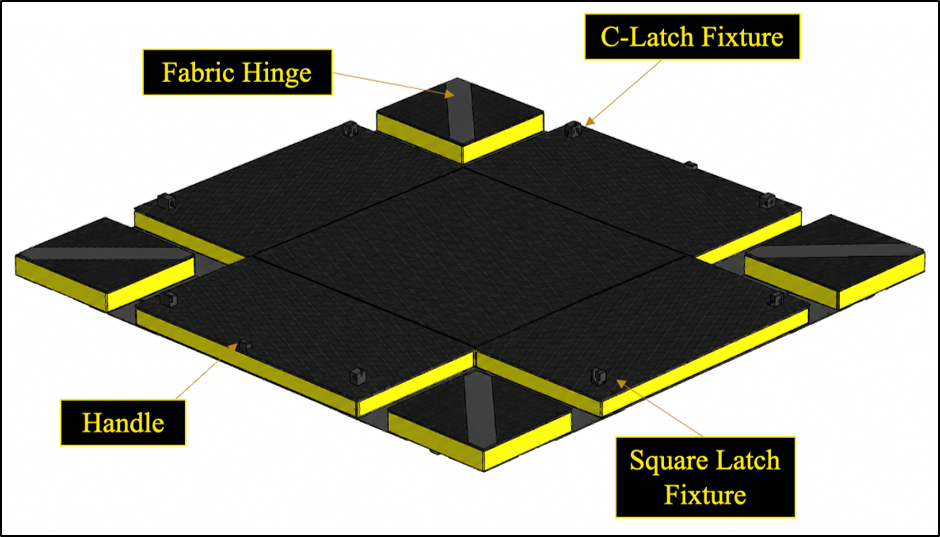
\includegraphics[
        width=1.92in,
        height=1.30in,
        keepaspectratio
    ]{toro_cover_underside_cad}
};
\draw[RuleGray,line width=0.55pt,rounded corners=4pt]
    ($(current page.north west)+(2.62in,-5.04in)$)
    rectangle
    ($(current page.north west)+(4.70in,-6.43in)$);

% Image 3: folded CAD
\node[anchor=center,inner sep=0pt]
at ($(current page.north west)+(5.85in,-5.73in)$)
{
    \includegraphics[
        width=1.92in,
        height=1.30in,
        keepaspectratio
    ]{\detokenize{Toro_Cover_folded Configuration}}
};
\draw[RuleGray,line width=0.55pt,rounded corners=4pt]
    ($(current page.north west)+(4.81in,-5.04in)$)
    rectangle
    ($(current page.north west)+(6.89in,-6.43in)$);

% Image 4: dual-use product concept
\node[anchor=center,inner sep=0pt]
at ($(current page.north west)+(8.04in,-5.73in)$)
{
    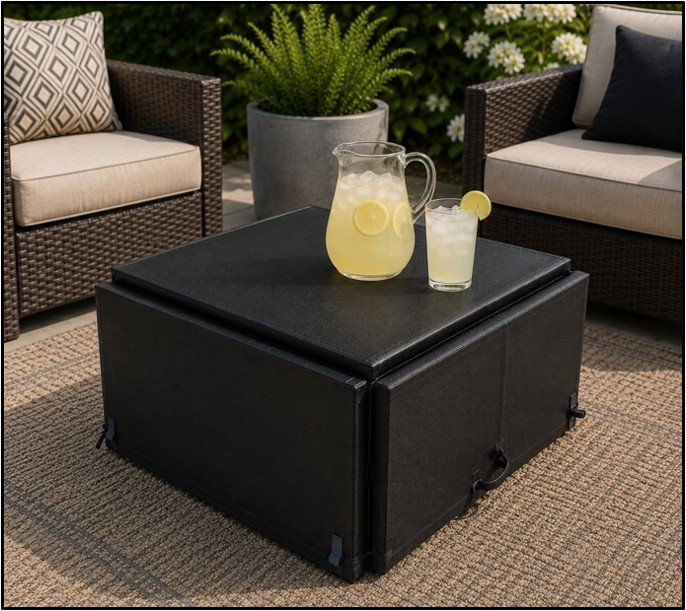
\includegraphics[
        width=1.92in,
        height=1.30in,
        keepaspectratio
    ]{generative_AI_concept_toro_cover_art}
};
\draw[RuleGray,line width=0.55pt,rounded corners=4pt]
    ($(current page.north west)+(7.00in,-5.04in)$)
    rectangle
    ($(current page.north west)+(9.08in,-6.43in)$);

% Image 5: folded foam functional prototype
% The portrait photograph is deliberately clipped to the landscape frame
% so the ottoman fills the card without extending beyond its border.
\begin{scope}
\clip[rounded corners=4pt]
    ($(current page.north west)+(9.19in,-5.04in)$)
    rectangle
    ($(current page.north east)+(-0.43in,-6.43in)$);

% Keep the original image proportions and center it within the existing card.
\node[anchor=center,inner sep=0pt]
at ($(current page.north west)+(9.88in,-5.735in)$)
{
    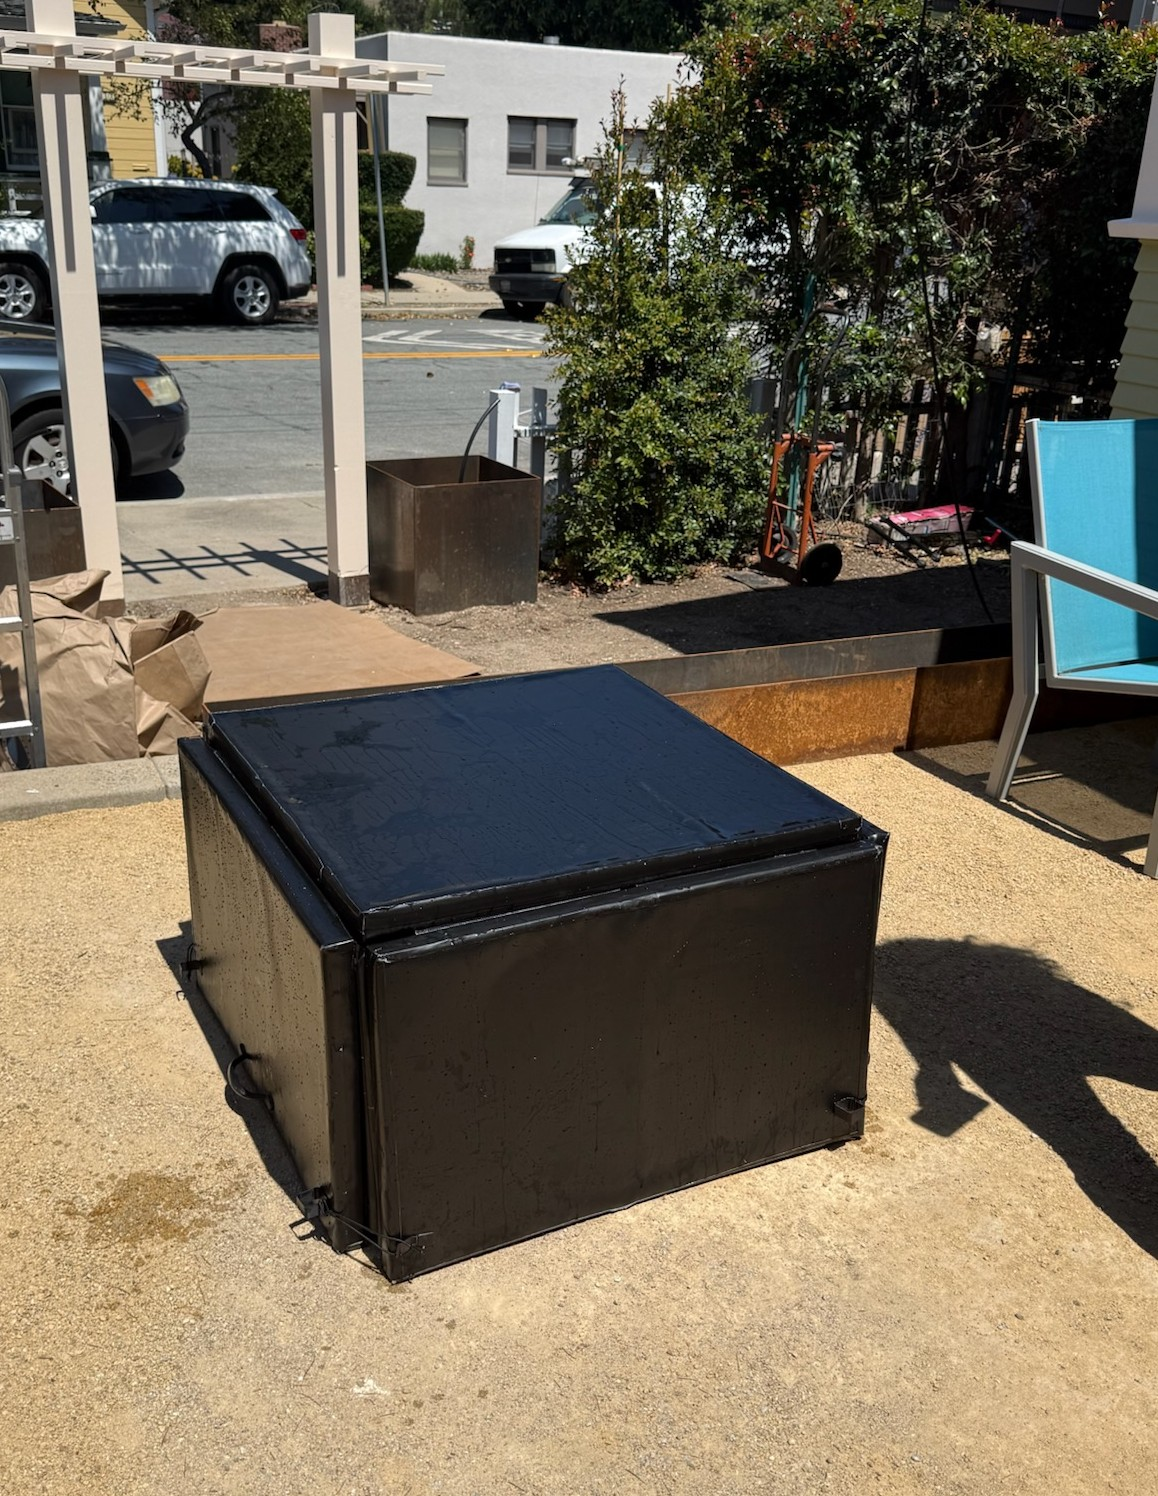
\includegraphics[
        width=1.58in,
        height=1.28in,
        keepaspectratio
    ]{foam_model_folded_backyard_image}
};
\end{scope}

\draw[RuleGray,line width=0.55pt,rounded corners=4pt]
    ($(current page.north west)+(9.19in,-5.04in)$)
    rectangle
    ($(current page.north east)+(-0.43in,-6.43in)$);

% Larger captions
\node[anchor=north,align=center,text width=1.95in,text=Muted,
      font=\sffamily\fontsize{6.8}{7.4}\selectfont]
at ($(current page.north west)+(1.47in,-6.49in)$)
{Topside panel architecture};

\node[anchor=north,align=center,text width=1.95in,text=Muted,
      font=\sffamily\fontsize{6.8}{7.4}\selectfont]
at ($(current page.north west)+(3.66in,-6.49in)$)
{Underside hinge architecture};

\node[anchor=north,align=center,text width=1.95in,text=Muted,
      font=\sffamily\fontsize{6.8}{7.4}\selectfont]
at ($(current page.north west)+(5.85in,-6.49in)$)
{Folded CAD configuration};

\node[anchor=north,align=center,text width=1.95in,text=Muted,
      font=\sffamily\fontsize{6.8}{7.4}\selectfont]
at ($(current page.north west)+(8.04in,-6.49in)$)
{Dual-use product vision};

\node[anchor=north,align=center,text width=1.95in,text=Muted,
      font=\sffamily\fontsize{6.8}{7.4}\selectfont]
at ($(current page.north west)+(9.88in,-6.49in)$)
{Folded foam prototype};

% Page 1 resource bar — centered and non-repeated resources
\fill[Panel,rounded corners=4pt]
    ($(current page.north west)+(0.43in,-7.05in)$)
    rectangle
    ($(current page.north east)+(-0.43in,-7.64in)$);
\draw[RuleGray,line width=0.5pt,rounded corners=4pt]
    ($(current page.north west)+(0.43in,-7.05in)$)
    rectangle
    ($(current page.north east)+(-0.43in,-7.64in)$);

\node[
    anchor=center,
    align=center,
    text=DeepGreen,
    font=\sffamily\bfseries\fontsize{6.9}{7.5}\selectfont
]
at ($(current page.north)+(0,-7.345in)$)
{\href{\ToroDrawingLink}{\faDraftingCompass\ DRAWING PACKAGE}
\hspace{24pt}
\href{\ToroDimensionsLink}{\faImage\ DIMENSION STUDY}
\hspace{24pt}
\href{\ToroProblemLink}{\faFileImage\ PROBLEM STATEMENT}};

% Footer
\node[
    anchor=south west,
    text=white,
    font=\sffamily\bfseries\fontsize{7.1}{7.7}\selectfont
]
at ($(current page.south west)+(0.42in,0.17in)$)
{\hyperlink{composites}{\faArrowLeft\ COMPOSITES}};

\node[
    anchor=south,
    text=white,
    font=\sffamily\fontsize{7.0}{7.6}\selectfont
]
at ($(current page.south)+(0,0.17in)$)
{TORO COVER \hspace{6pt} 1 / 3};

\node[
    anchor=south east,
    text=white,
    font=\sffamily\bfseries\fontsize{7.1}{7.7}\selectfont
]
at ($(current page.south east)+(-0.42in,0.17in)$)
{MANUFACTURING-DRIVEN DESIGN \faArrowRight};

\end{tikzpicture}


% ============================================================
% PAGE 2 — MANUFACTURING-DRIVEN DESIGN
% ============================================================

\clearpage
\thispagestyle{empty}
\hypertarget{toro-manufacturing}{}
\null

\begin{tikzpicture}[remember picture,overlay]

% Background and bars
\fill[white]
    (current page.south west)
    rectangle
    (current page.north east);

\fill[DeepGreen]
    (current page.north west)
    rectangle
    ($(current page.north east)+(0,-0.095in)$);

\fill[PolyGold]
    ($(current page.north west)+(0,-0.095in)$)
    rectangle
    ($(current page.north east)+(0,-0.14in)$);

\fill[DeepGreen]
    (current page.south west)
    rectangle
    ($(current page.south east)+(0,0.36in)$);

\fill[PolyGold]
    ($(current page.south west)+(0,0.36in)$)
    rectangle
    ($(current page.south east)+(0,0.405in)$);

% Header
\node[
    anchor=north west,
    text=PolyGold,
    font=\sffamily\bfseries\fontsize{8.1}{8.7}\selectfont
]
at ($(current page.north west)+(0.42in,-0.39in)$)
{TORO COVER \hspace{5pt}/\hspace{5pt} DESIGN FOR MANUFACTURABILITY};

\node[
    anchor=north west,
    text=DeepGreen,
    font=\bfseries\fontsize{23}{24}\selectfont
]
at ($(current page.north west)+(0.40in,-0.67in)$)
{THE ENVELOPE METHOD};

\node[
    anchor=north west,
    text=Muted,
    font=\sffamily\fontsize{8.7}{9.6}\selectfont
]
at ($(current page.north west)+(0.42in,-1.12in)$)
{A one-layup process developed for unusually thick insulated composite sandwich panels};

\fill[PolyGold]
    ($(current page.north west)+(0.42in,-1.36in)$)
    rectangle
    ($(current page.north west)+(5.30in,-1.315in)$);

% Process explanation
\fill[SoftGold,rounded corners=5pt]
    ($(current page.north west)+(0.42in,-1.61in)$)
    rectangle
    ($(current page.north east)+(-0.42in,-2.90in)$);

\fill[PolyGold]
    ($(current page.north west)+(0.42in,-1.61in)$)
    rectangle
    ($(current page.north west)+(0.52in,-2.90in)$);

\node[
    anchor=north west,
    text=DeepGreen,
    font=\sffamily\bfseries\fontsize{7.9}{8.6}\selectfont
]
at ($(current page.north west)+(0.67in,-1.76in)$)
{PROCESS INNOVATION};

\node[
    anchor=north west,
    align=left,
    text width=9.55in,
    text=Ink,
    font=\fontsize{7.35}{8.75}\selectfont
]
at ($(current page.north west)+(0.67in,-2.02in)$)
{
Weight reduction and insulation were both essential, leading to the selection of an
XPS foam core. Because XPS could not tolerate composite heat-cure temperatures, prepreg
processing was not practical and the panels had to be manufactured by wet layup with a
room-temperature cure. To simplify this process, I waterjet-cut XPS perimeter strips from
excess foam and placed them around each core inside the vacuum enclosure. Under vacuum,
the top and bottom carbon skins met along the panel sides and compressed against this
border, eliminating a separate edge-banding layup and reducing corner pleating.
};

% Workflow title
\node[
    anchor=north west,
    text=DeepGreen,
    font=\sffamily\bfseries\fontsize{8.0}{8.7}\selectfont
]
at ($(current page.north west)+(0.43in,-3.06in)$)
{MANUFACTURING WORKFLOW};

% Row 1 image 1
\node[anchor=center,inner sep=0pt]
at ($(current page.north west)+(2.07in,-4.105in)$)
{
    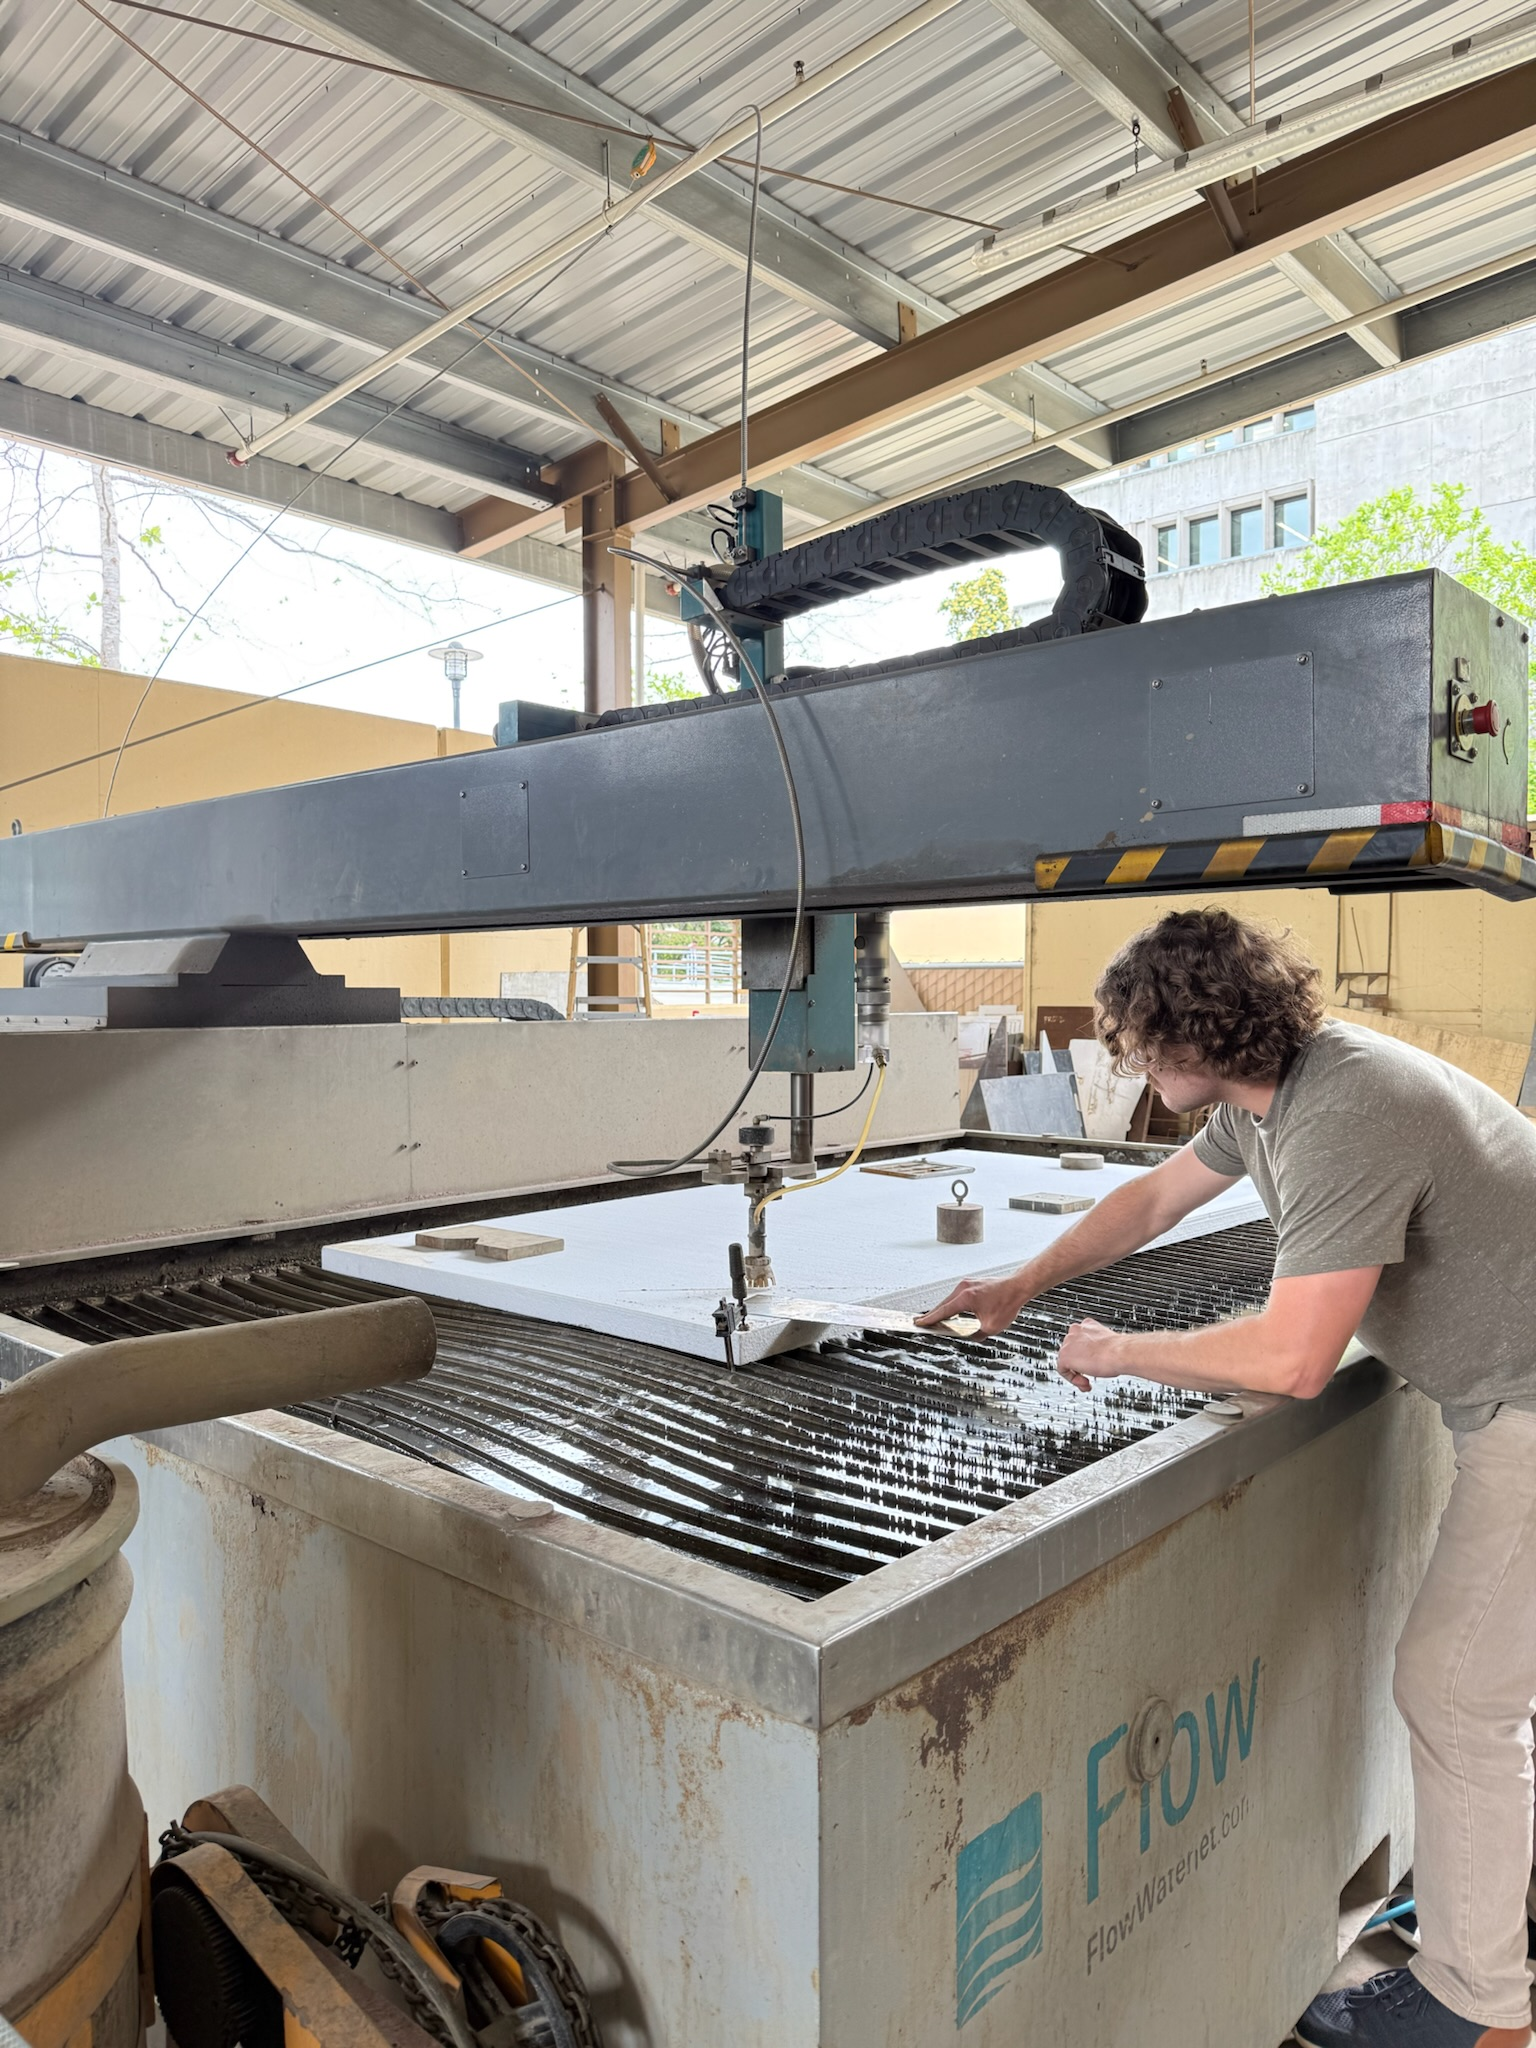
\includegraphics[
        width=3.10in,
        height=1.40in,
        keepaspectratio
    ]{waterjet_foam}
};
\draw[RuleGray,line width=0.55pt,rounded corners=4pt]
    ($(current page.north west)+(0.43in,-3.36in)$)
    rectangle
    ($(current page.north west)+(3.71in,-4.85in)$);

% Row 1 image 2
\node[anchor=center,inner sep=0pt]
at ($(current page.north west)+(5.50in,-4.105in)$)
{
    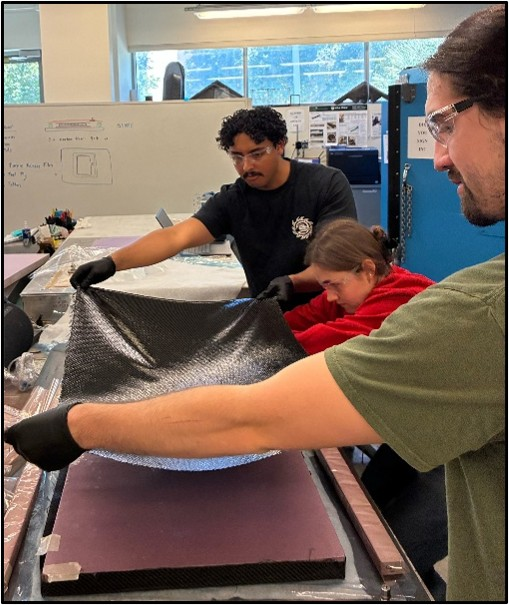
\includegraphics[
        width=3.10in,
        height=1.40in,
        keepaspectratio
    ]{group_layup}
};
\draw[RuleGray,line width=0.55pt,rounded corners=4pt]
    ($(current page.north west)+(3.86in,-3.36in)$)
    rectangle
    ($(current page.north west)+(7.14in,-4.85in)$);

% Row 1 image 3
\node[anchor=center,inner sep=0pt]
at ($(current page.north west)+(8.935in,-4.105in)$)
{
    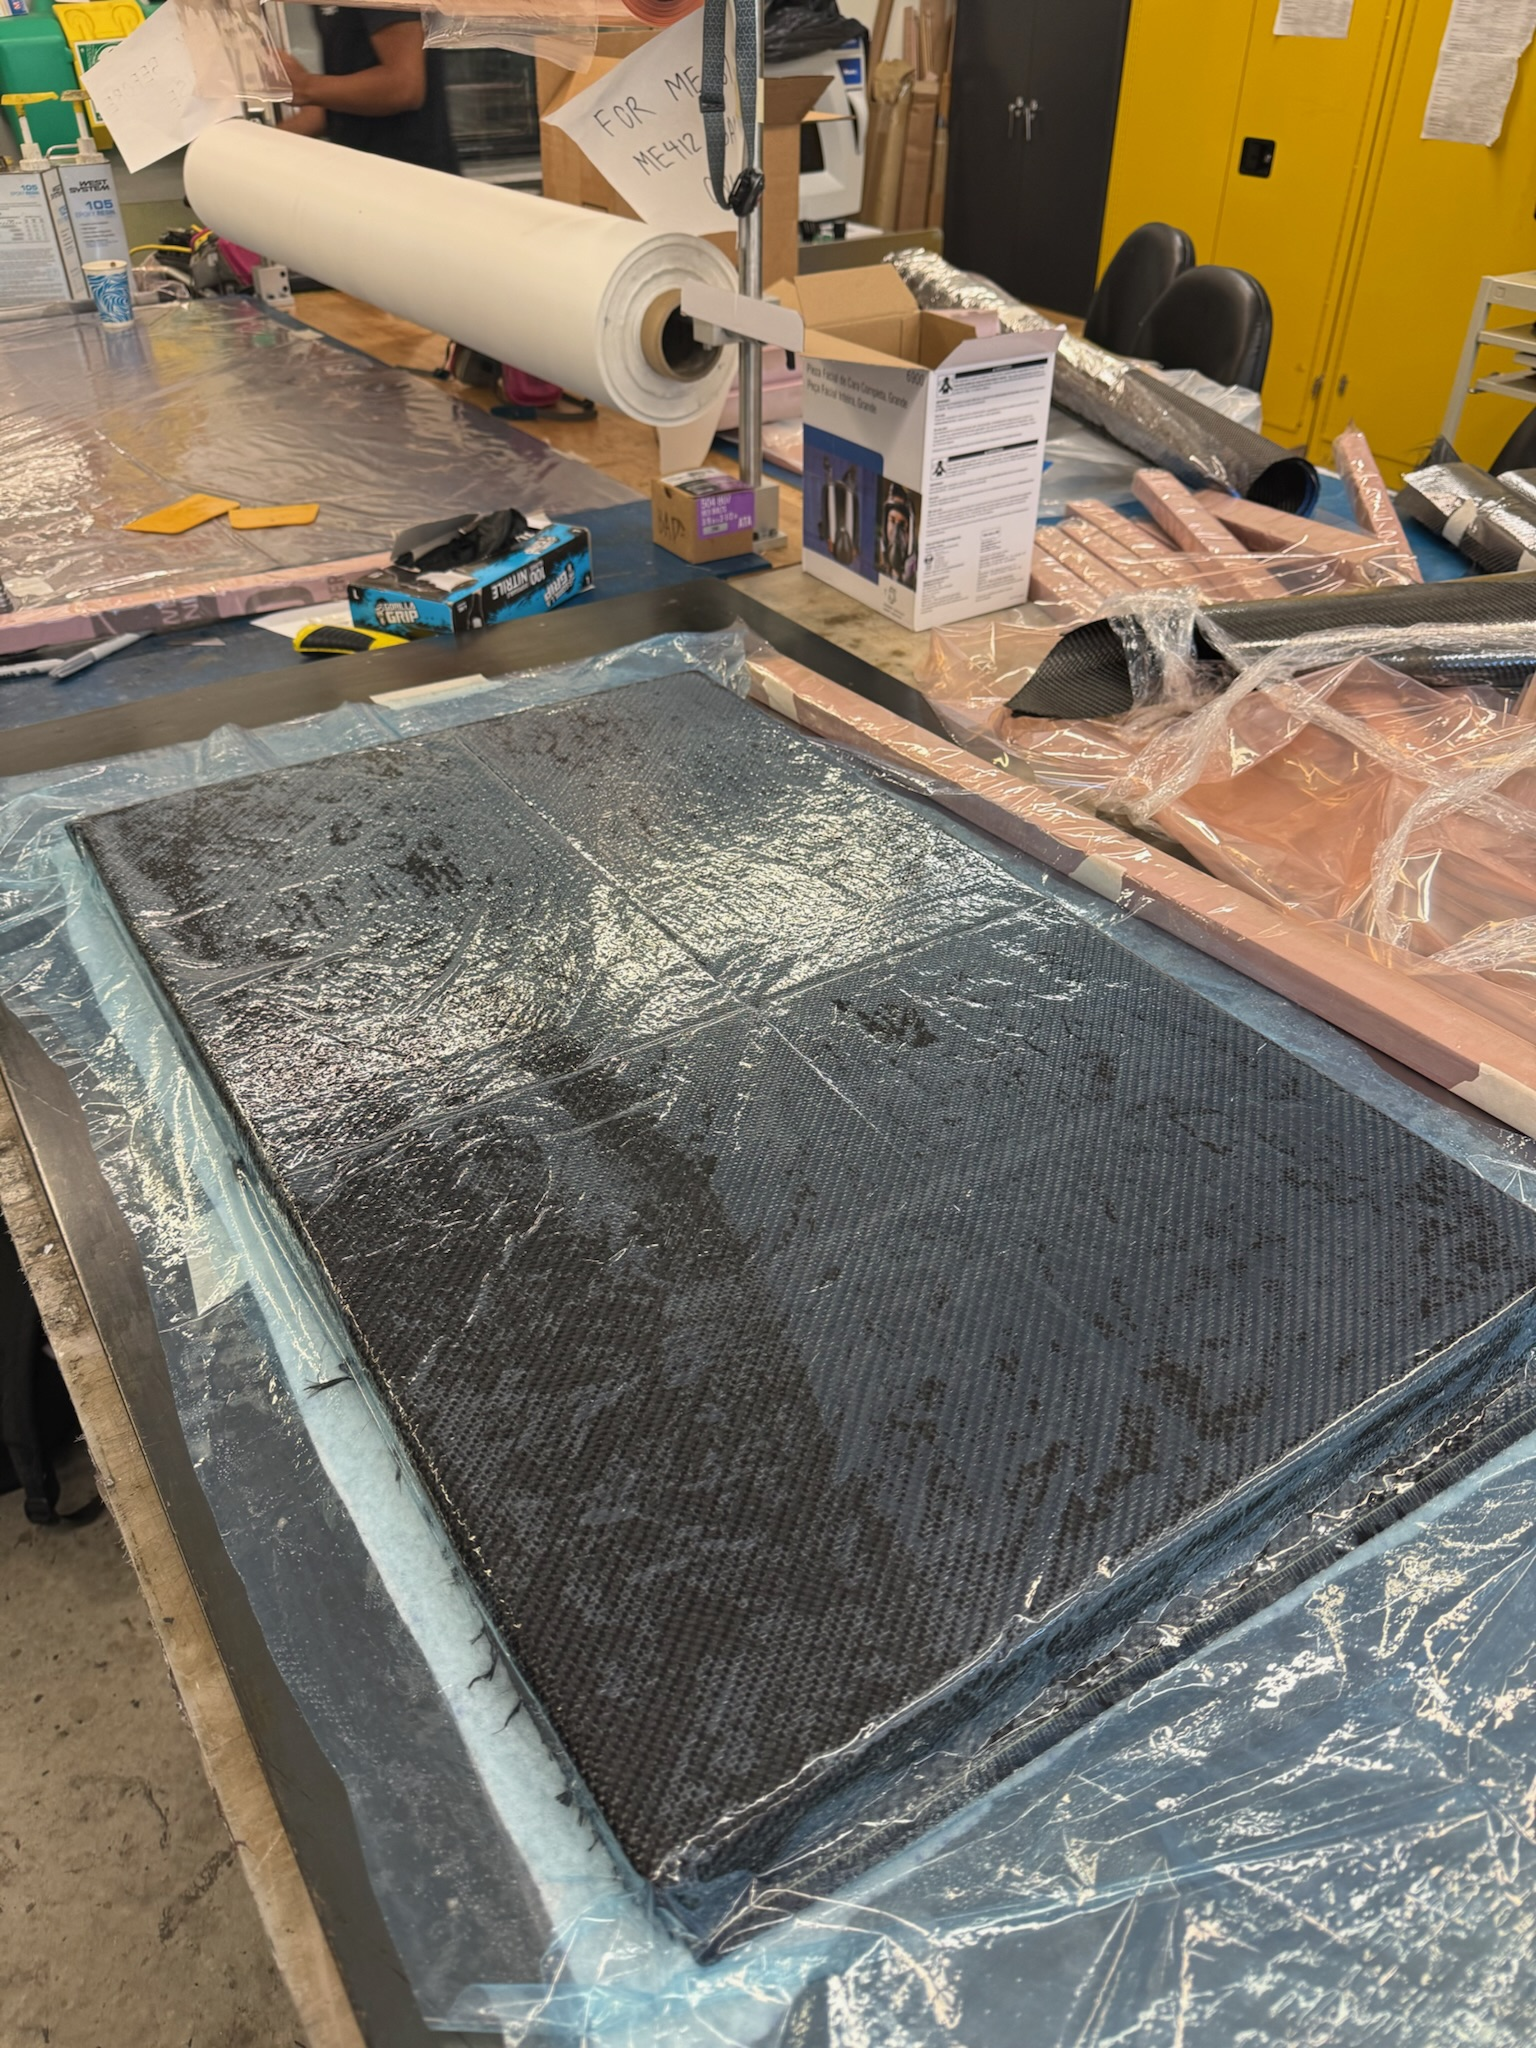
\includegraphics[
        width=3.10in,
        height=1.40in,
        keepaspectratio
    ]{blue_perforrated_film_layup}
};
\draw[RuleGray,line width=0.55pt,rounded corners=4pt]
    ($(current page.north west)+(7.29in,-3.36in)$)
    rectangle
    ($(current page.north east)+(-0.42in,-4.85in)$);

% Row 1 captions
\node[anchor=north,text=Muted,font=\sffamily\fontsize{6.7}{7.3}\selectfont]
at ($(current page.north west)+(2.07in,-4.90in)$)
{1. Waterjet-cut core and perimeter geometry};

\node[anchor=north,text=Muted,font=\sffamily\fontsize{6.7}{7.3}\selectfont]
at ($(current page.north west)+(5.50in,-4.90in)$)
{2. Team wet layup under my process guidance};

\node[anchor=north,text=Muted,font=\sffamily\fontsize{6.7}{7.3}\selectfont]
at ($(current page.north west)+(8.935in,-4.90in)$)
{3. Perforated film, breather, and vacuum enclosure};

% Row 2 image 1
\node[anchor=center,inner sep=0pt]
at ($(current page.north west)+(2.07in,-5.875in)$)
{
    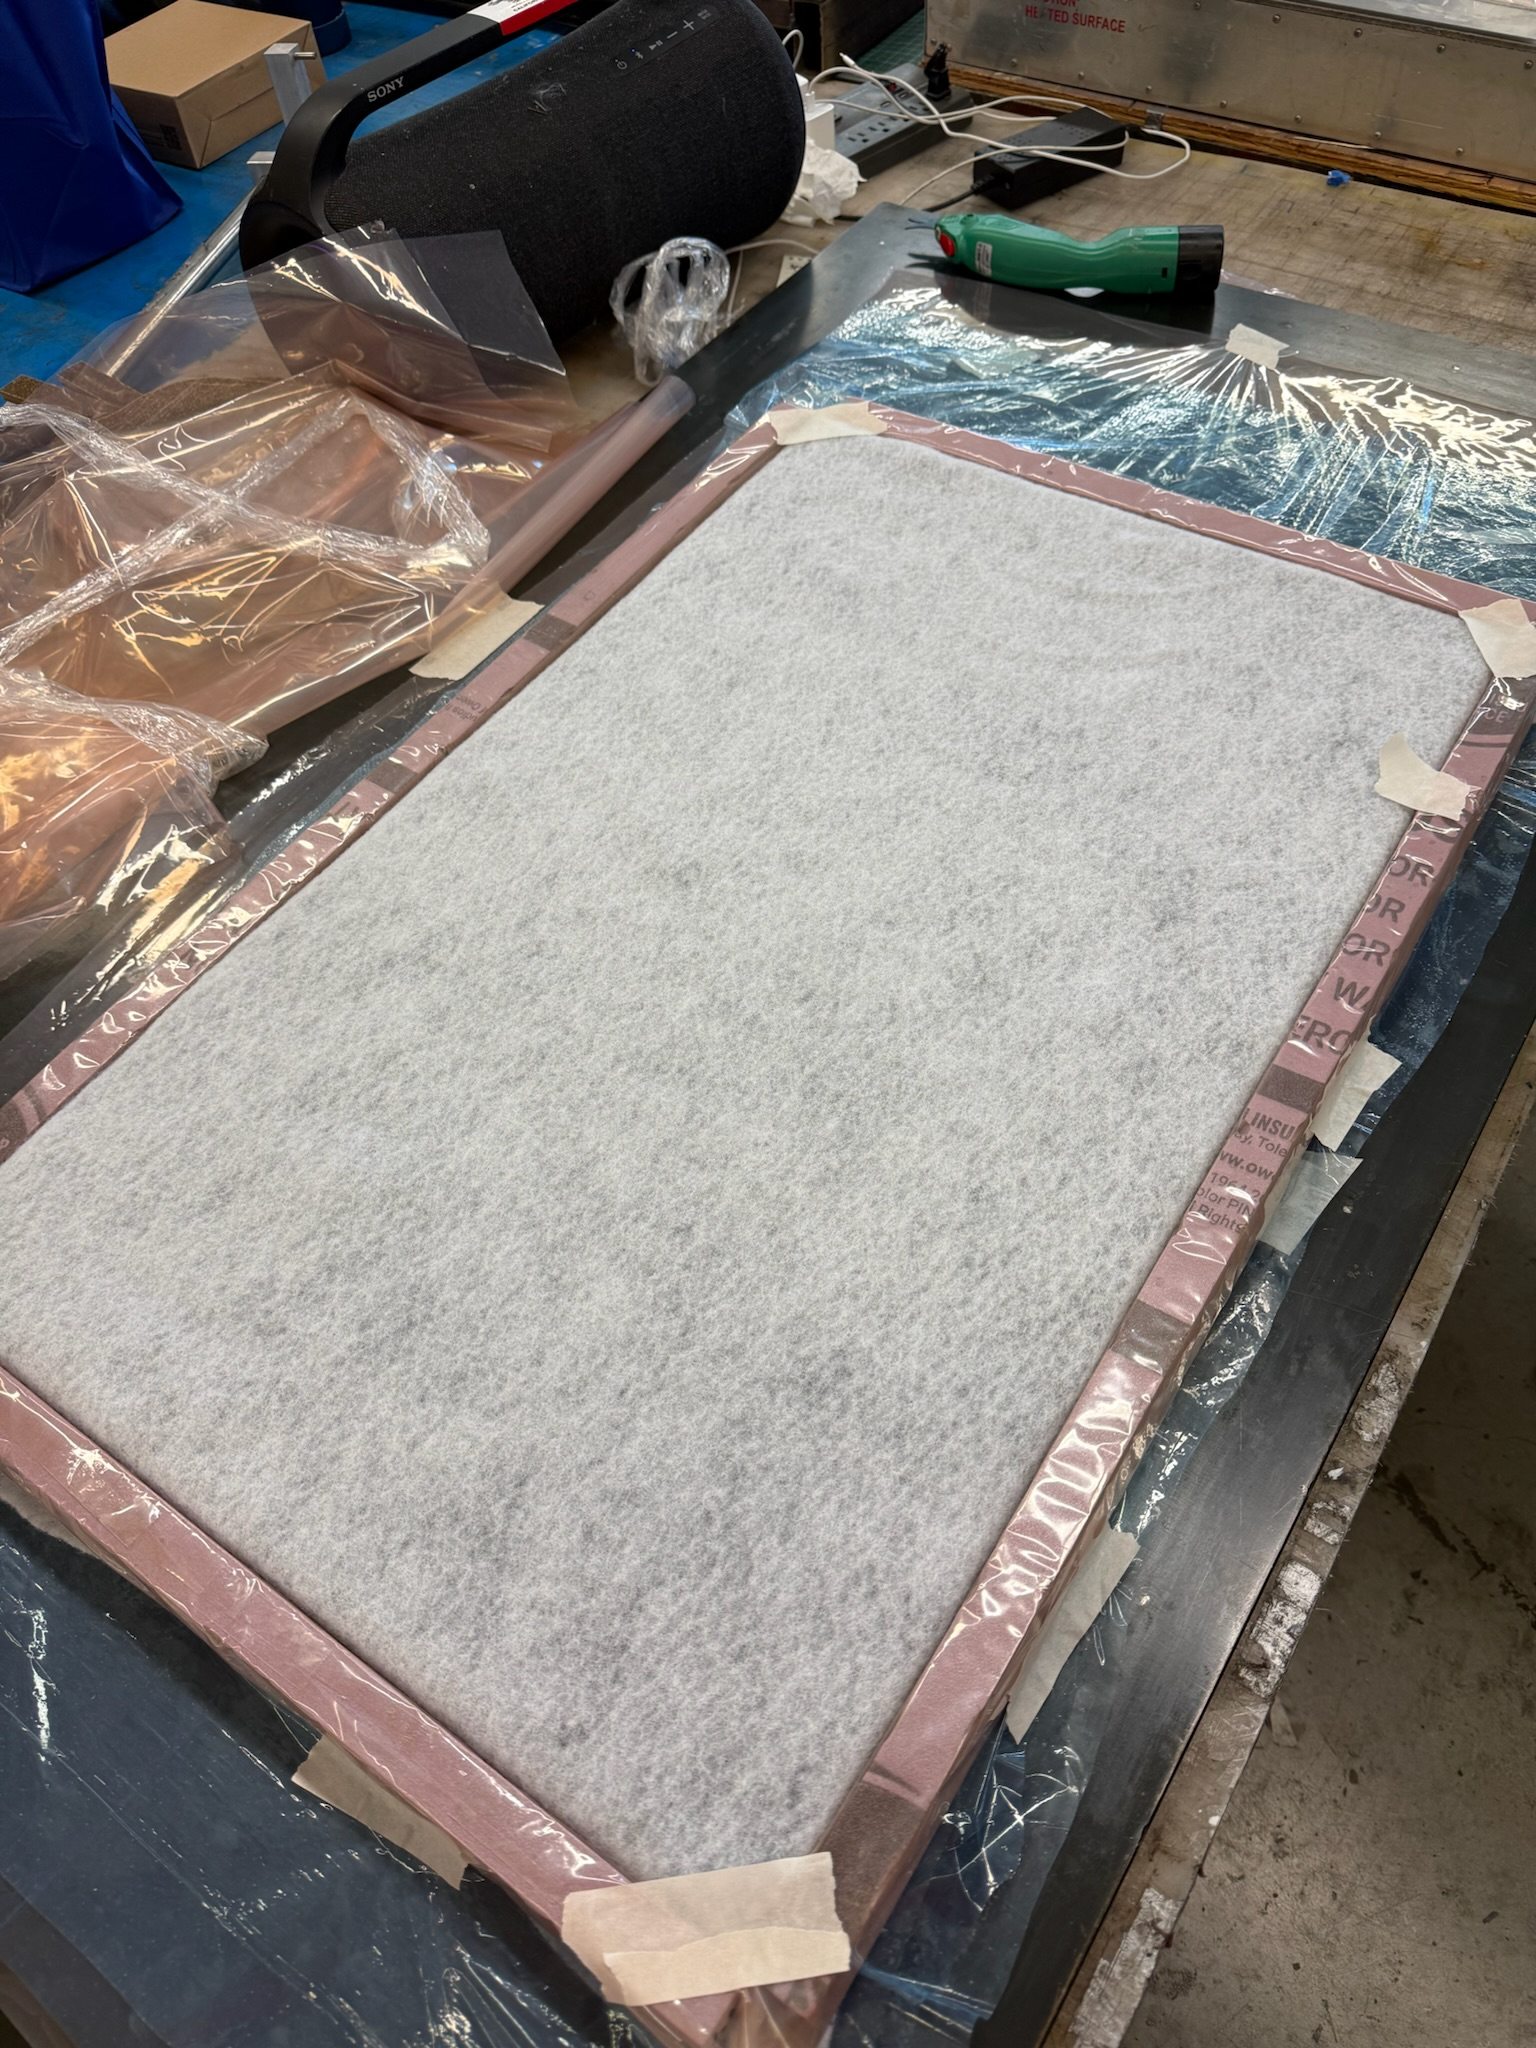
\includegraphics[
        width=3.10in,
        height=1.40in,
        keepaspectratio
    ]{completed_layup}
};
\draw[RuleGray,line width=0.55pt,rounded corners=4pt]
    ($(current page.north west)+(0.43in,-5.13in)$)
    rectangle
    ($(current page.north west)+(3.71in,-6.62in)$);

% Row 2 image 2 — oven chamber used only as a reliable vacuum enclosure; no heat applied
\node[anchor=center,inner sep=0pt]
at ($(current page.north west)+(5.50in,-5.875in)$)
{
    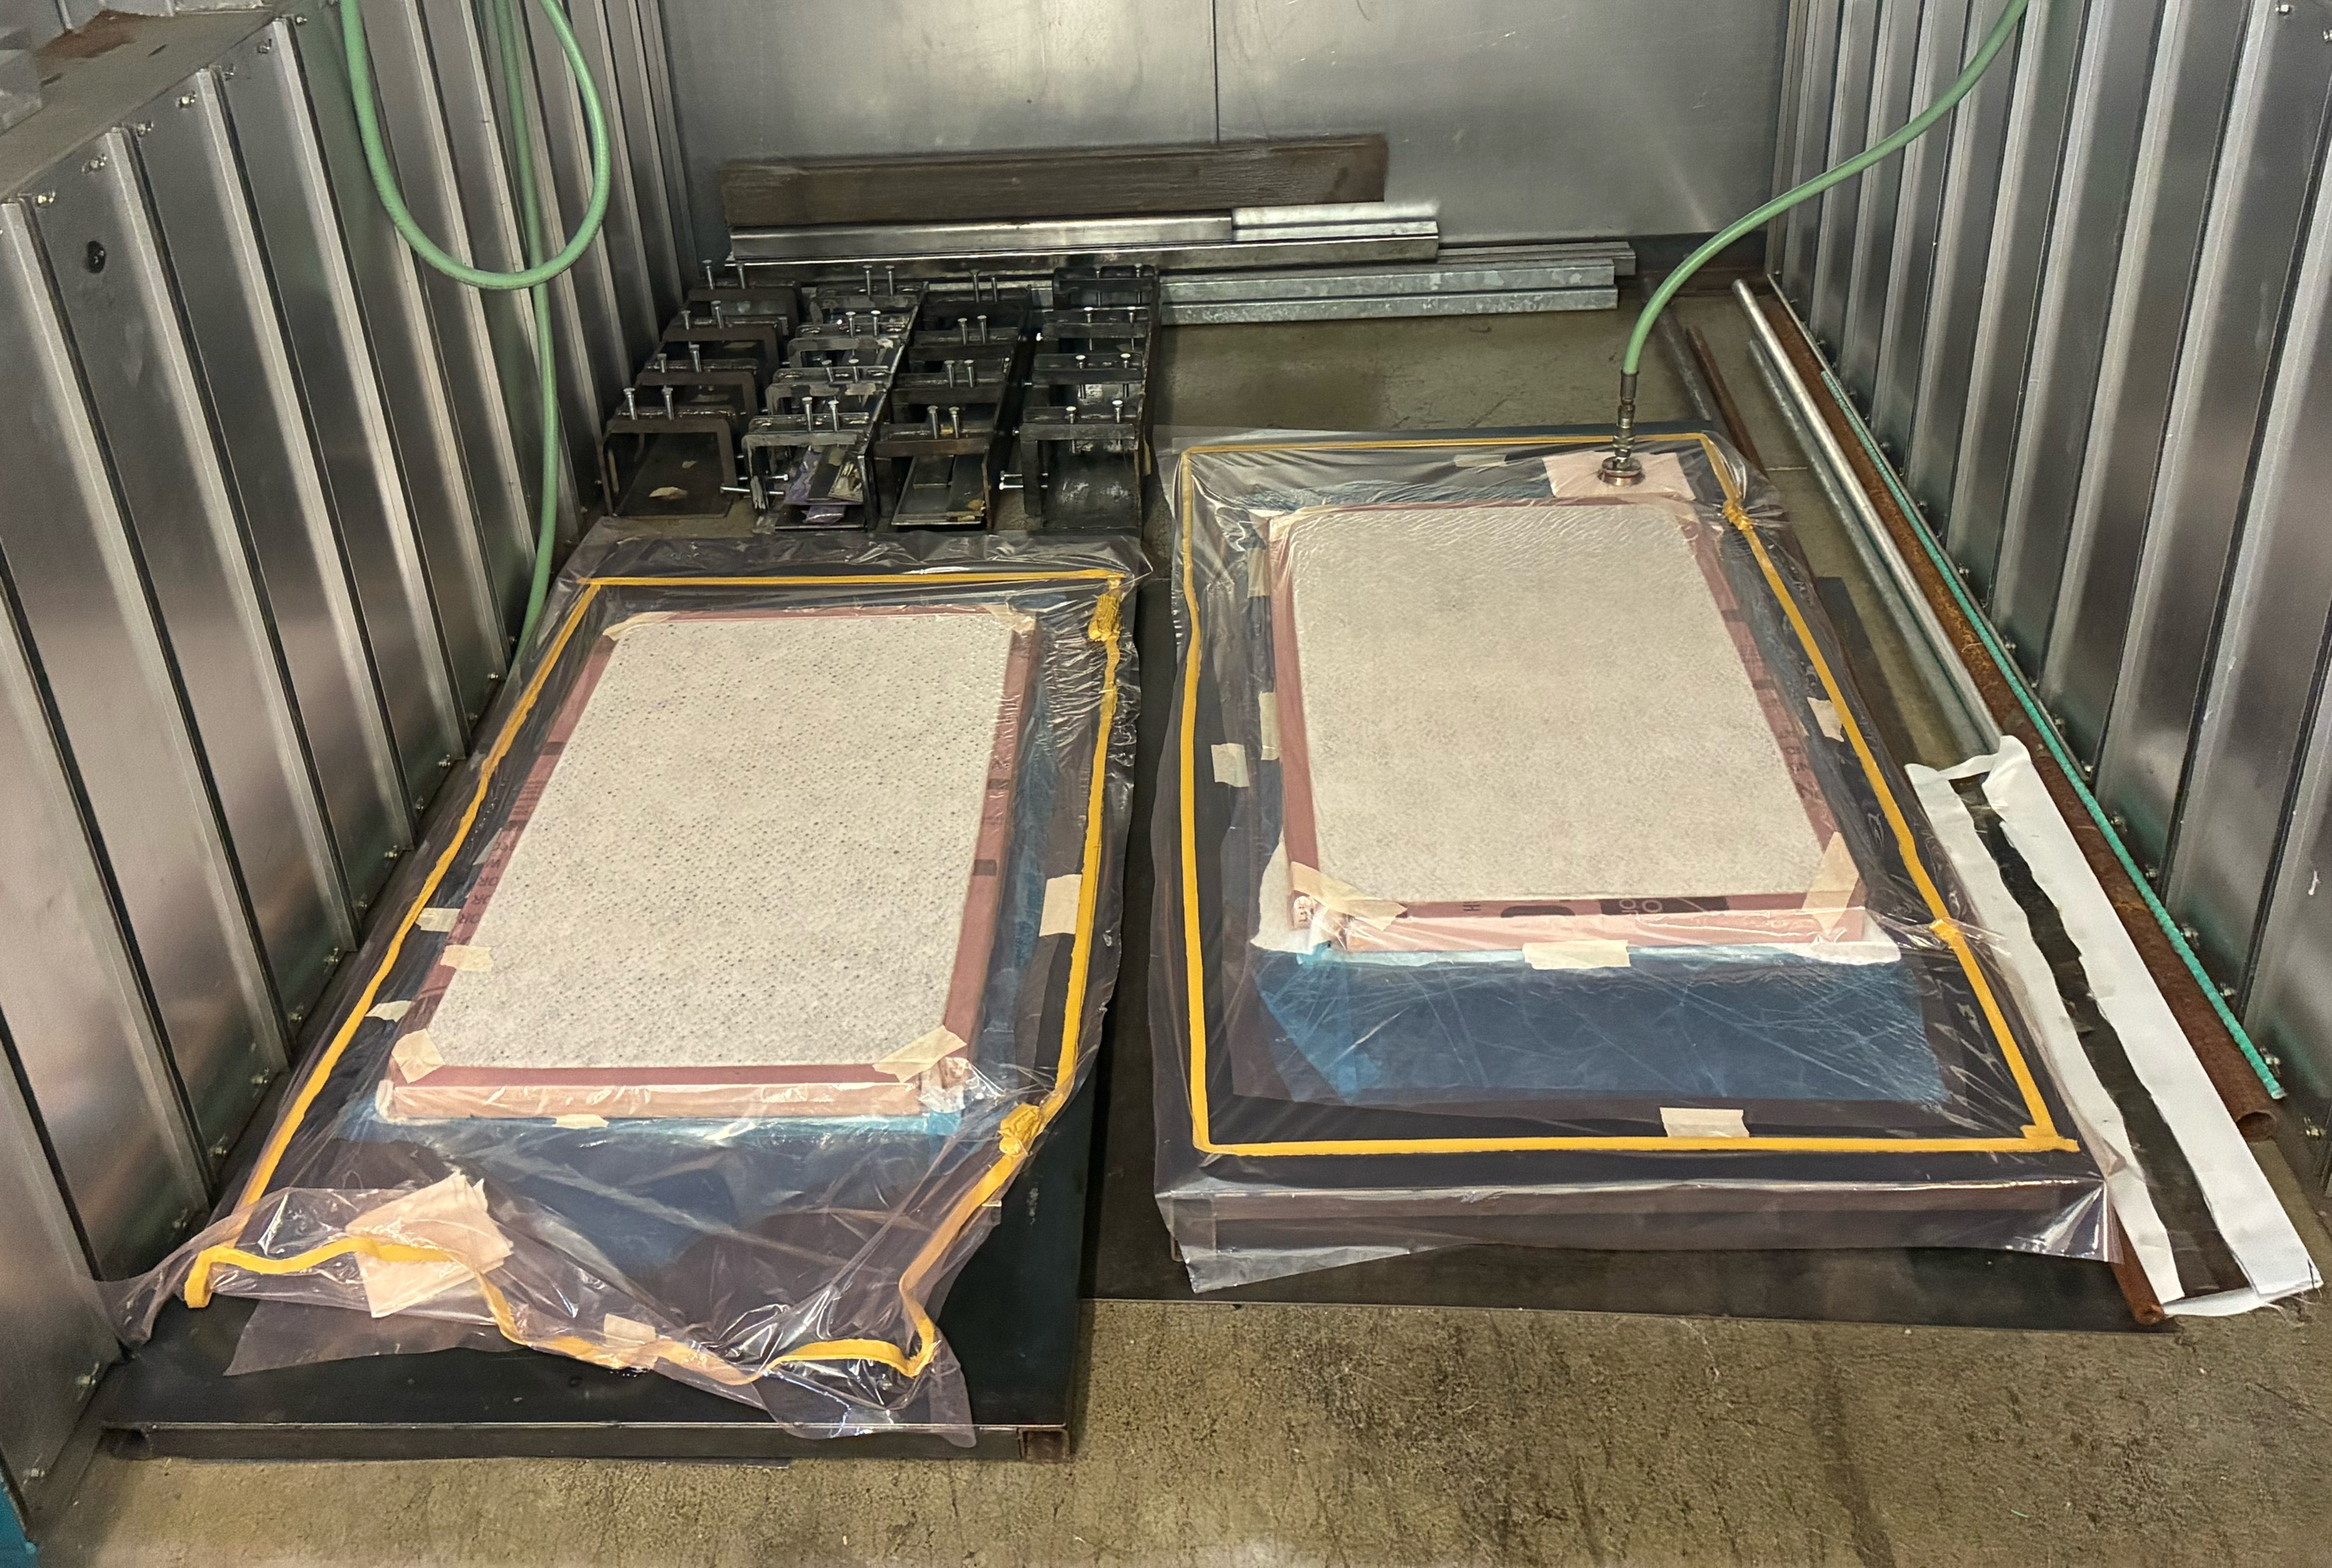
\includegraphics[
        width=3.10in,
        height=1.40in,
        keepaspectratio
    ]{layups_in_composite_oven_under_vacuumPressure}
};
\draw[RuleGray,line width=0.55pt,rounded corners=4pt]
    ($(current page.north west)+(3.86in,-5.13in)$)
    rectangle
    ($(current page.north west)+(7.14in,-6.62in)$);

% Row 2 image 3
\node[anchor=center,inner sep=0pt]
at ($(current page.north west)+(8.935in,-5.875in)$)
{
    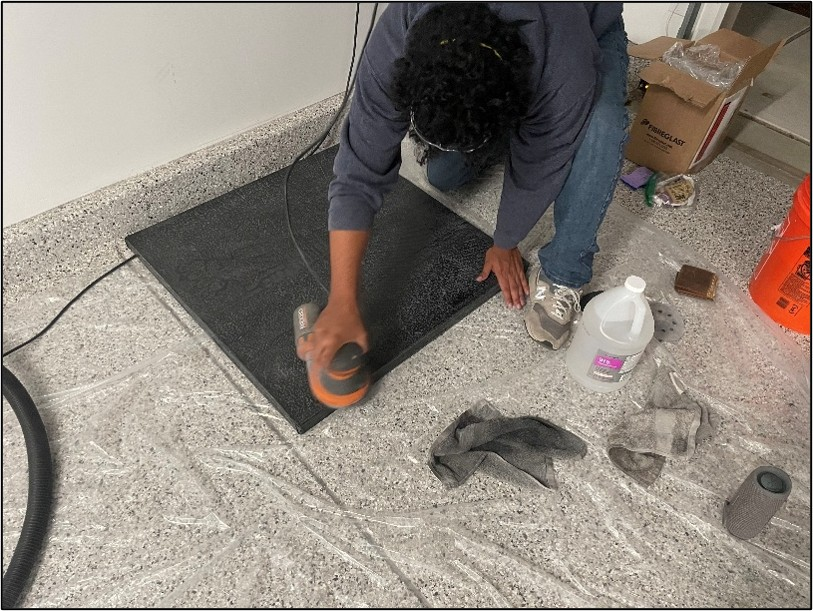
\includegraphics[
        width=3.10in,
        height=1.40in,
        keepaspectratio
    ]{garage_sanding}
};
\draw[RuleGray,line width=0.55pt,rounded corners=4pt]
    ($(current page.north west)+(7.29in,-5.13in)$)
    rectangle
    ($(current page.north east)+(-0.42in,-6.62in)$);

% Row 2 captions
\node[anchor=north,text=Muted,font=\sffamily\fontsize{6.7}{7.3}\selectfont]
at ($(current page.north west)+(2.07in,-6.67in)$)
{4. Fully saturated carbon skin and foam sandwich};

\node[anchor=north,text=Muted,font=\sffamily\fontsize{6.7}{7.3}\selectfont]
at ($(current page.north west)+(5.50in,-6.67in)$)
{5. Room-temperature cure under continuous vacuum};

\node[anchor=north,text=Muted,font=\sffamily\fontsize{6.7}{7.3}\selectfont]
at ($(current page.north west)+(8.935in,-6.67in)$)
{6. Post-processing and surface preparation};

% Bottom callouts
\fill[Panel,rounded corners=4pt]
    ($(current page.north west)+(0.43in,-6.95in)$)
    rectangle
    ($(current page.north west)+(5.48in,-7.60in)$);

\draw[RuleGray,line width=0.55pt,rounded corners=4pt]
    ($(current page.north west)+(0.43in,-6.95in)$)
    rectangle
    ($(current page.north west)+(5.48in,-7.60in)$);

\node[
    anchor=north west,
    text=DeepGreen,
    font=\sffamily\bfseries\fontsize{7.0}{7.6}\selectfont
]
at ($(current page.north west)+(0.63in,-7.08in)$)
{FROM THREE LAYUPS TO ONE};

\node[
    anchor=north west,
    align=left,
    text width=4.56in,
    text=Ink,
    font=\fontsize{6.45}{7.45}\selectfont
]
at ($(current page.north west)+(0.63in,-7.29in)$)
{
The Envelope Method reduced labor, cure cycles, handling,
alignment risk, and time spent forming numerous vacuum-bag
pleats around the 1.5-inch-thick XPS panels.
};

\fill[Panel,rounded corners=4pt]
    ($(current page.north west)+(5.68in,-6.95in)$)
    rectangle
    ($(current page.north east)+(-0.42in,-7.60in)$);

\draw[RuleGray,line width=0.55pt,rounded corners=4pt]
    ($(current page.north west)+(5.68in,-6.95in)$)
    rectangle
    ($(current page.north east)+(-0.42in,-7.60in)$);

\node[
    anchor=north west,
    text=DeepGreen,
    font=\sffamily\bfseries\fontsize{7.0}{7.6}\selectfont
]
at ($(current page.north west)+(5.88in,-7.08in)$)
{WHY SURFACE-BONDED HARDWARE};

\node[
    anchor=north west,
    align=left,
    text width=4.55in,
    text=Ink,
    font=\fontsize{6.45}{7.45}\selectfont
]
at ($(current page.north west)+(5.88in,-7.29in)$)
{
Adhesively bonded hinges and fixtures preserved the clean
composite exterior and avoided drilled inserts, foam-core
crushing, added stress concentrations, and new leak paths.
};


% Footer
\node[
    anchor=south west,
    text=white,
    font=\sffamily\bfseries\fontsize{7.1}{7.7}\selectfont
]
at ($(current page.south west)+(0.42in,0.17in)$)
{\faArrowLeft\ PRODUCT ARCHITECTURE};

\node[
    anchor=south,
    text=white,
    font=\sffamily\fontsize{7.0}{7.6}\selectfont
]
at ($(current page.south)+(0,0.17in)$)
{TORO COVER \hspace{6pt} 2 / 3};

\node[
    anchor=south east,
    text=white,
    font=\sffamily\bfseries\fontsize{7.1}{7.7}\selectfont
]
at ($(current page.south east)+(-0.42in,0.17in)$)
{VALIDATION \& TAKEAWAYS \faArrowRight};

\end{tikzpicture}


% ============================================================
% PAGE 3 — FINISHING, VALIDATION, AND TAKEAWAYS
% ============================================================

\clearpage
\thispagestyle{empty}
\hypertarget{toro-results}{}
\null

\begin{tikzpicture}[remember picture,overlay]

% Background and bars
\fill[white]
    (current page.south west)
    rectangle
    (current page.north east);

\fill[DeepGreen]
    (current page.north west)
    rectangle
    ($(current page.north east)+(0,-0.095in)$);

\fill[PolyGold]
    ($(current page.north west)+(0,-0.095in)$)
    rectangle
    ($(current page.north east)+(0,-0.14in)$);

\fill[DeepGreen]
    (current page.south west)
    rectangle
    ($(current page.south east)+(0,0.36in)$);

\fill[PolyGold]
    ($(current page.south west)+(0,0.36in)$)
    rectangle
    ($(current page.south east)+(0,0.405in)$);

% Header
\node[
    anchor=north west,
    text=PolyGold,
    font=\sffamily\bfseries\fontsize{8.1}{8.7}\selectfont
]
at ($(current page.north west)+(0.42in,-0.39in)$)
{TORO COVER \hspace{5pt}/\hspace{5pt} VALIDATION AND ENGINEERING TAKEAWAYS};

\node[
    anchor=north west,
    text=DeepGreen,
    font=\bfseries\fontsize{22.5}{23.5}\selectfont
]
at ($(current page.north west)+(0.40in,-0.67in)$)
{FROM PROTOTYPE TO PRODUCT PATHWAY};

\node[
    anchor=north west,
    text=Muted,
    font=\sffamily\fontsize{8.7}{9.6}\selectfont
]
at ($(current page.north west)+(0.42in,-1.12in)$)
{Environmental protection, usability testing, scope decisions, and lessons from technical leadership};

\fill[PolyGold]
    ($(current page.north west)+(0.42in,-1.36in)$)
    rectangle
    ($(current page.north west)+(5.8in,-1.315in)$);

% Finishing title
\node[
    anchor=north west,
    text=DeepGreen,
    font=\sffamily\bfseries\fontsize{8.0}{8.7}\selectfont
]
at ($(current page.north west)+(0.43in,-1.62in)$)
{OUTDOOR FINISHING AND ENVIRONMENTAL PROTECTION};

% Image 1
\node[anchor=center,inner sep=0pt]
at ($(current page.north west)+(1.705in,-2.655in)$)
{
    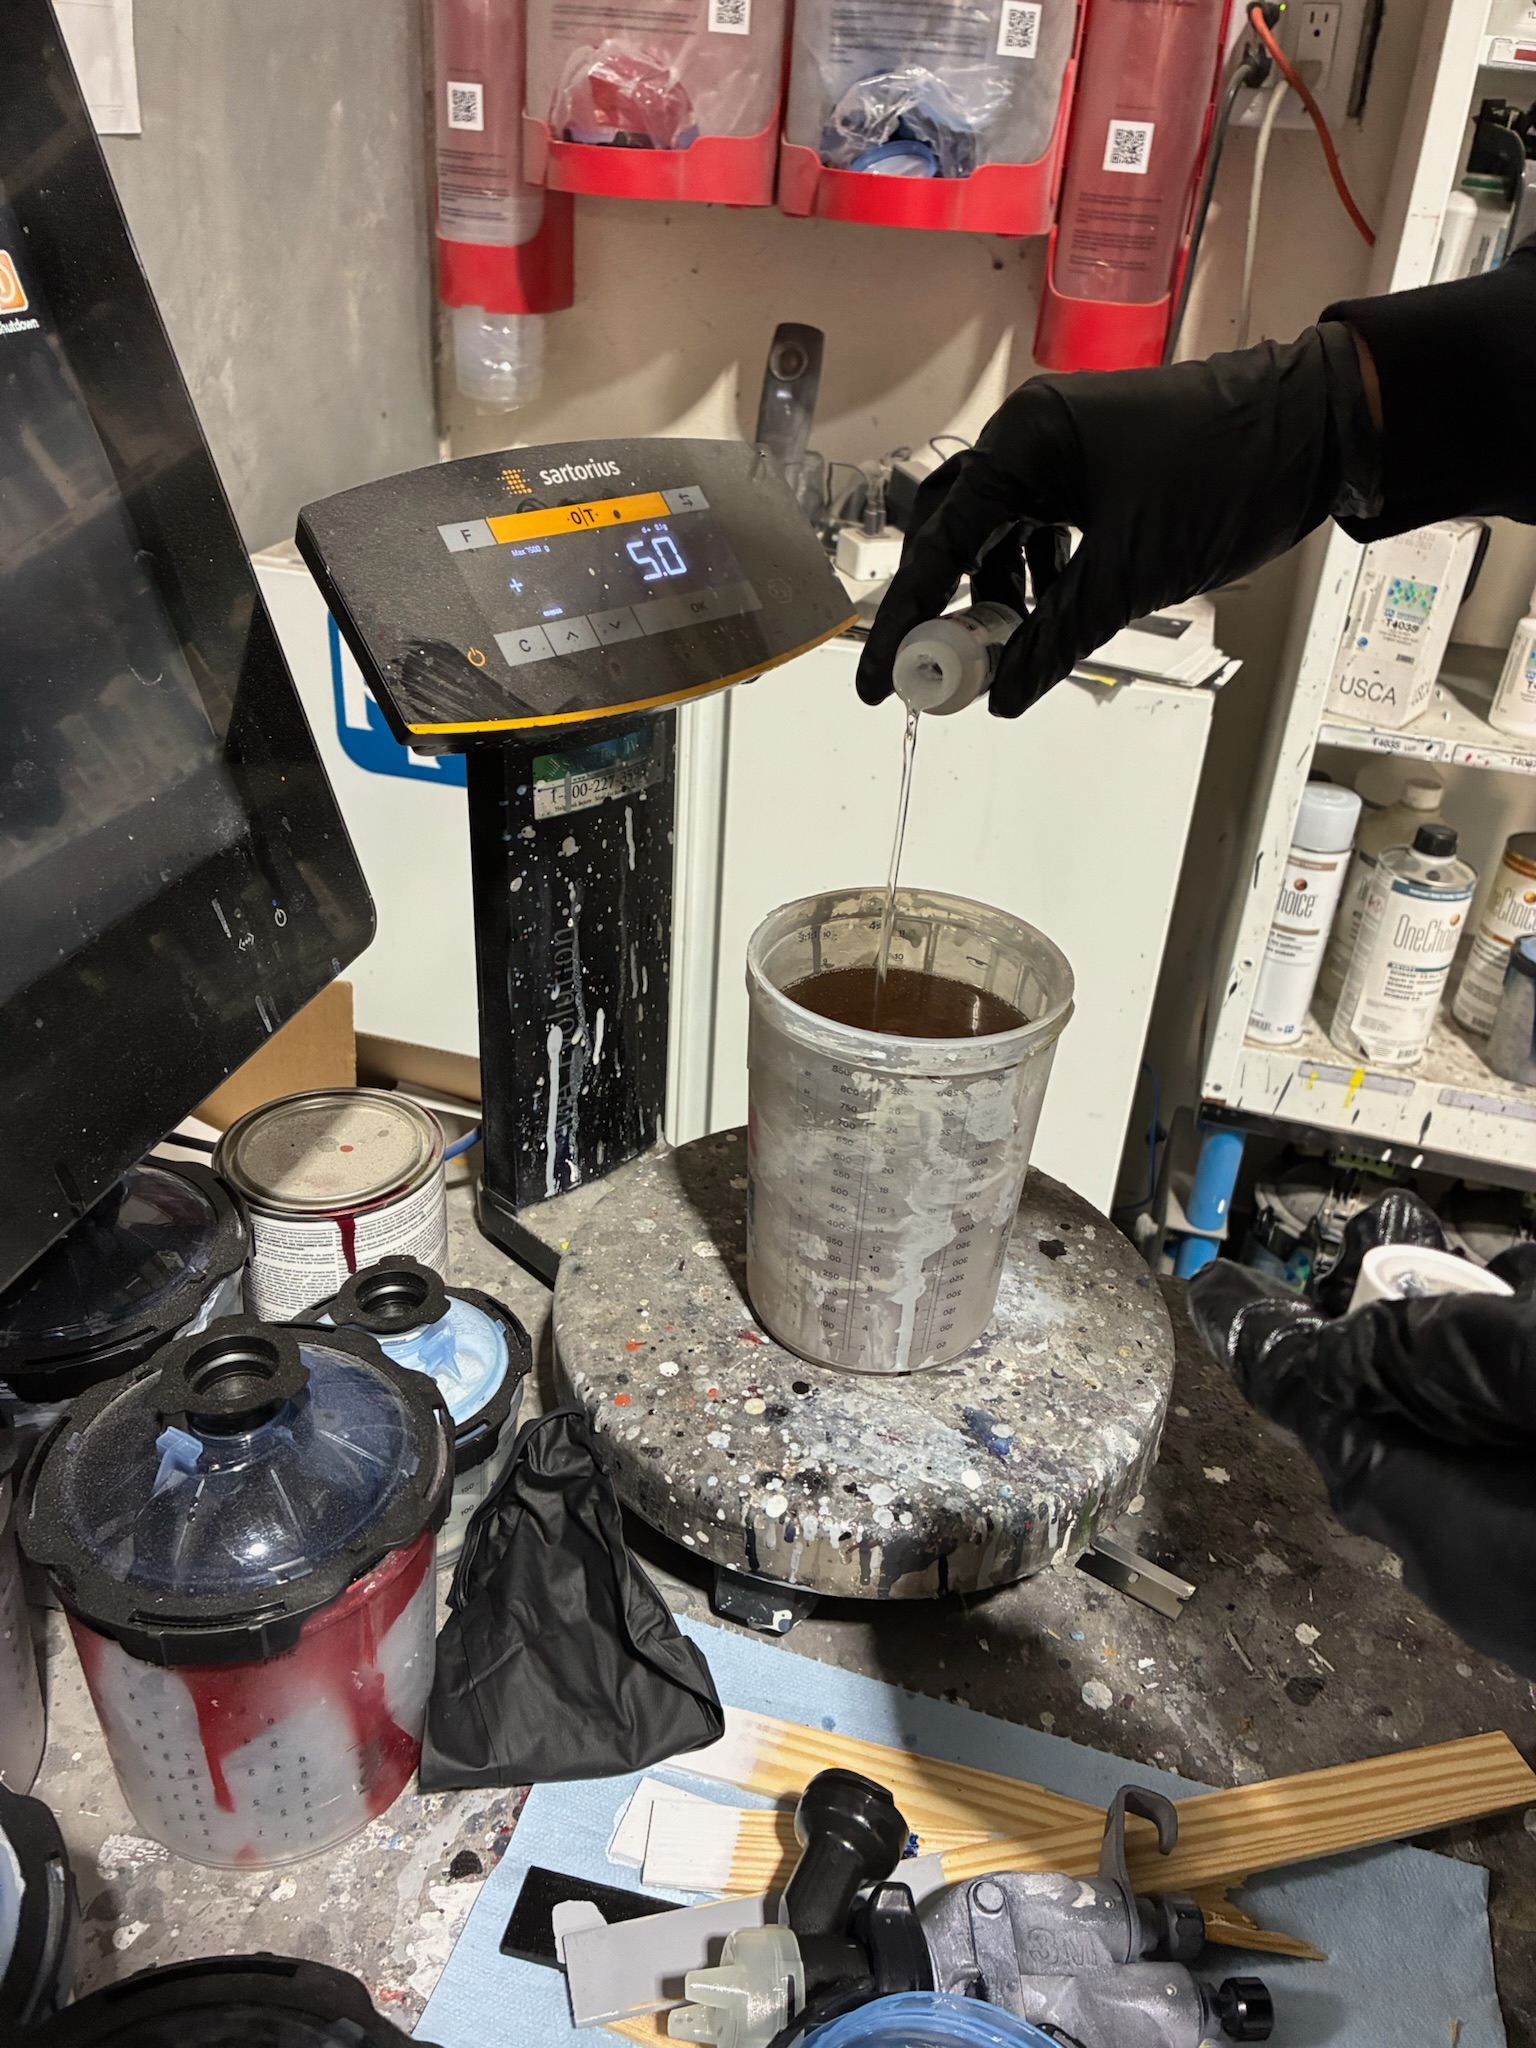
\includegraphics[
        width=2.35in,
        height=1.40in,
        keepaspectratio
    ]{spray_topcoat_prep}
};
\draw[RuleGray,line width=0.55pt,rounded corners=4pt]
    ($(current page.north west)+(0.43in,-1.91in)$)
    rectangle
    ($(current page.north west)+(2.98in,-3.40in)$);

% Image 2
\node[anchor=center,inner sep=0pt]
at ($(current page.north west)+(4.375in,-2.655in)$)
{
    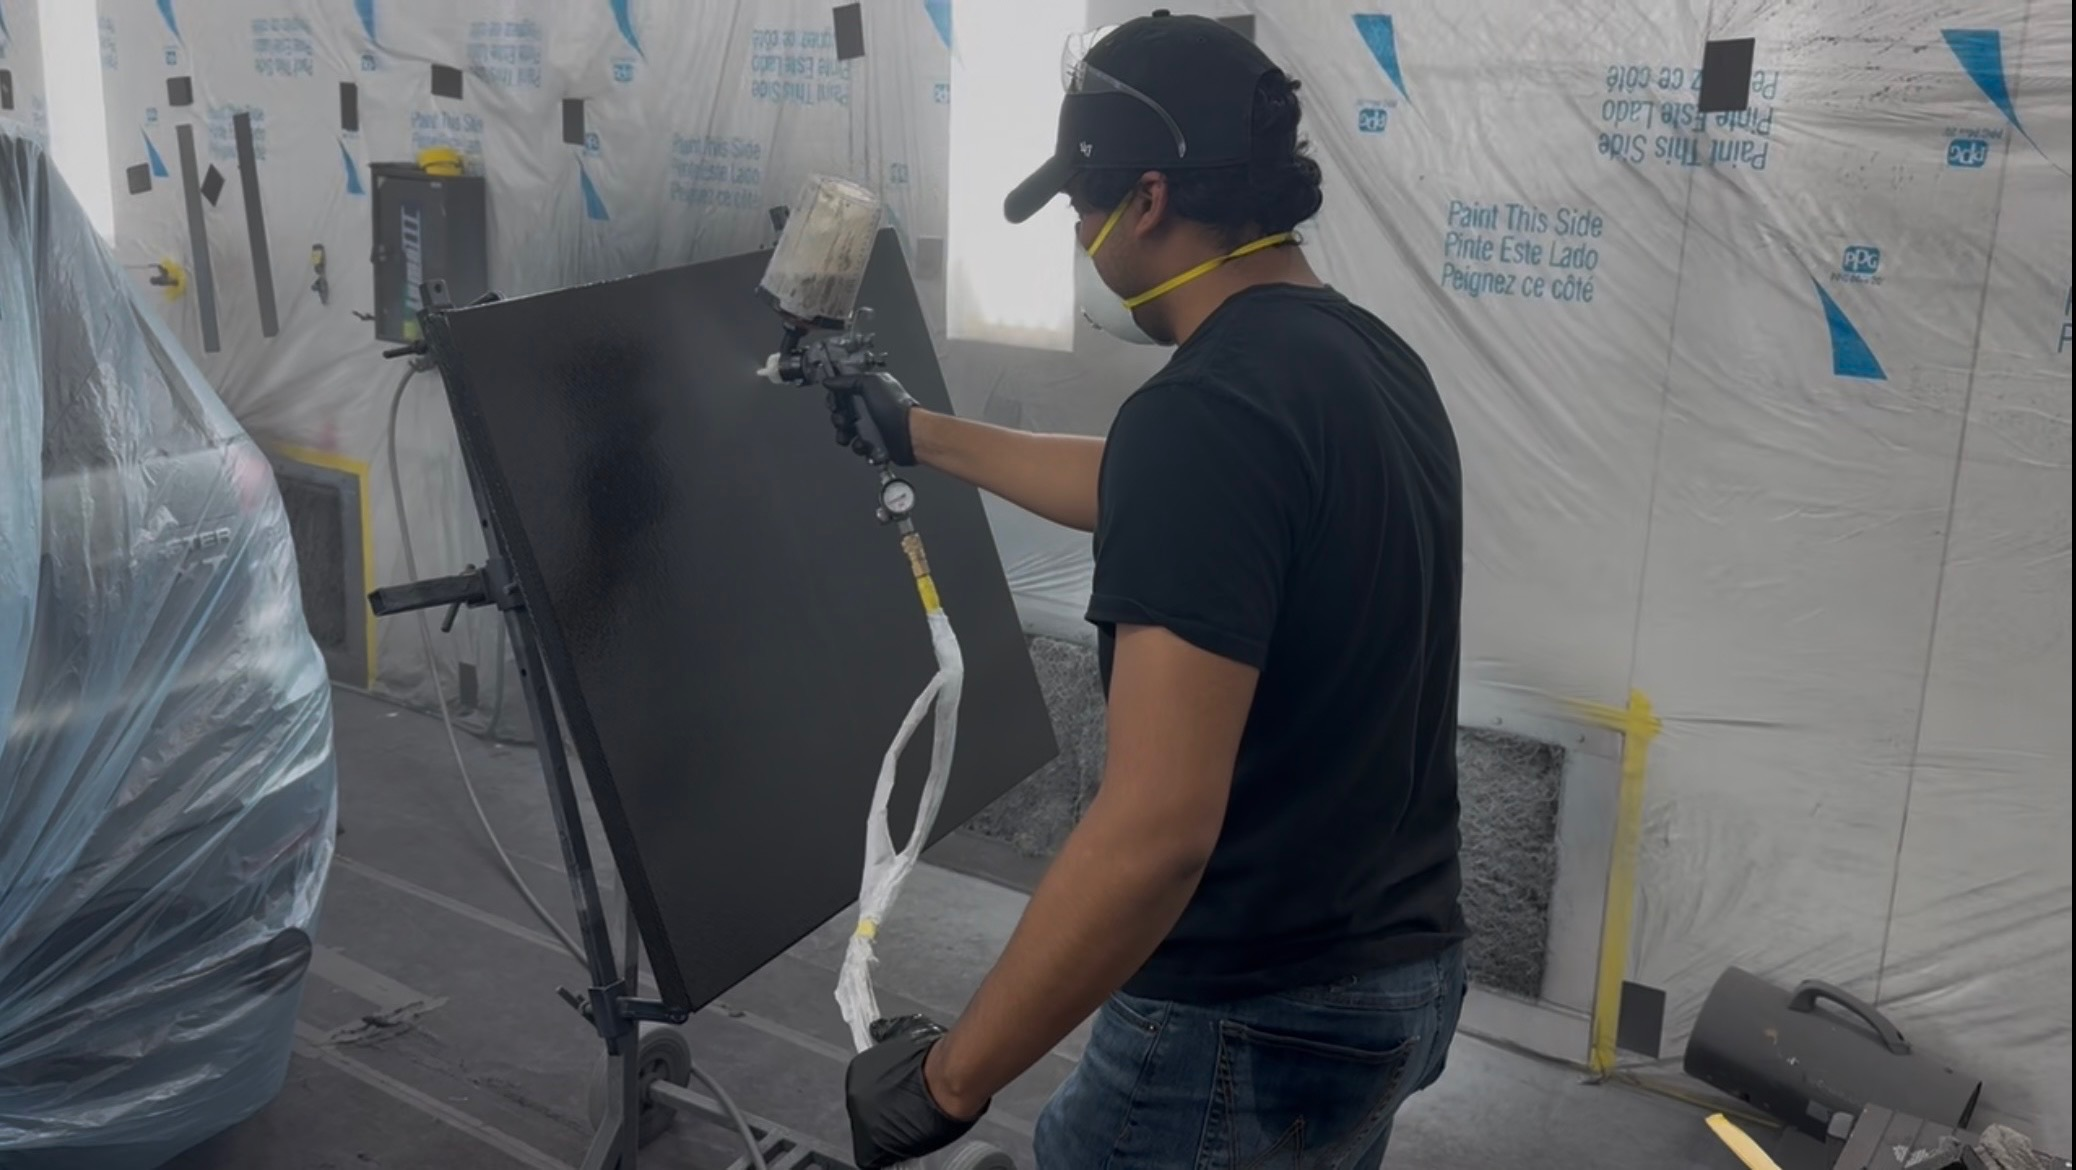
\includegraphics[
        width=2.35in,
        height=1.40in,
        keepaspectratio
    ]{spraying_topcoat}
};
\draw[RuleGray,line width=0.55pt,rounded corners=4pt]
    ($(current page.north west)+(3.10in,-1.91in)$)
    rectangle
    ($(current page.north west)+(5.65in,-3.40in)$);

% Image 3
\node[anchor=center,inner sep=0pt]
at ($(current page.north west)+(7.045in,-2.655in)$)
{
    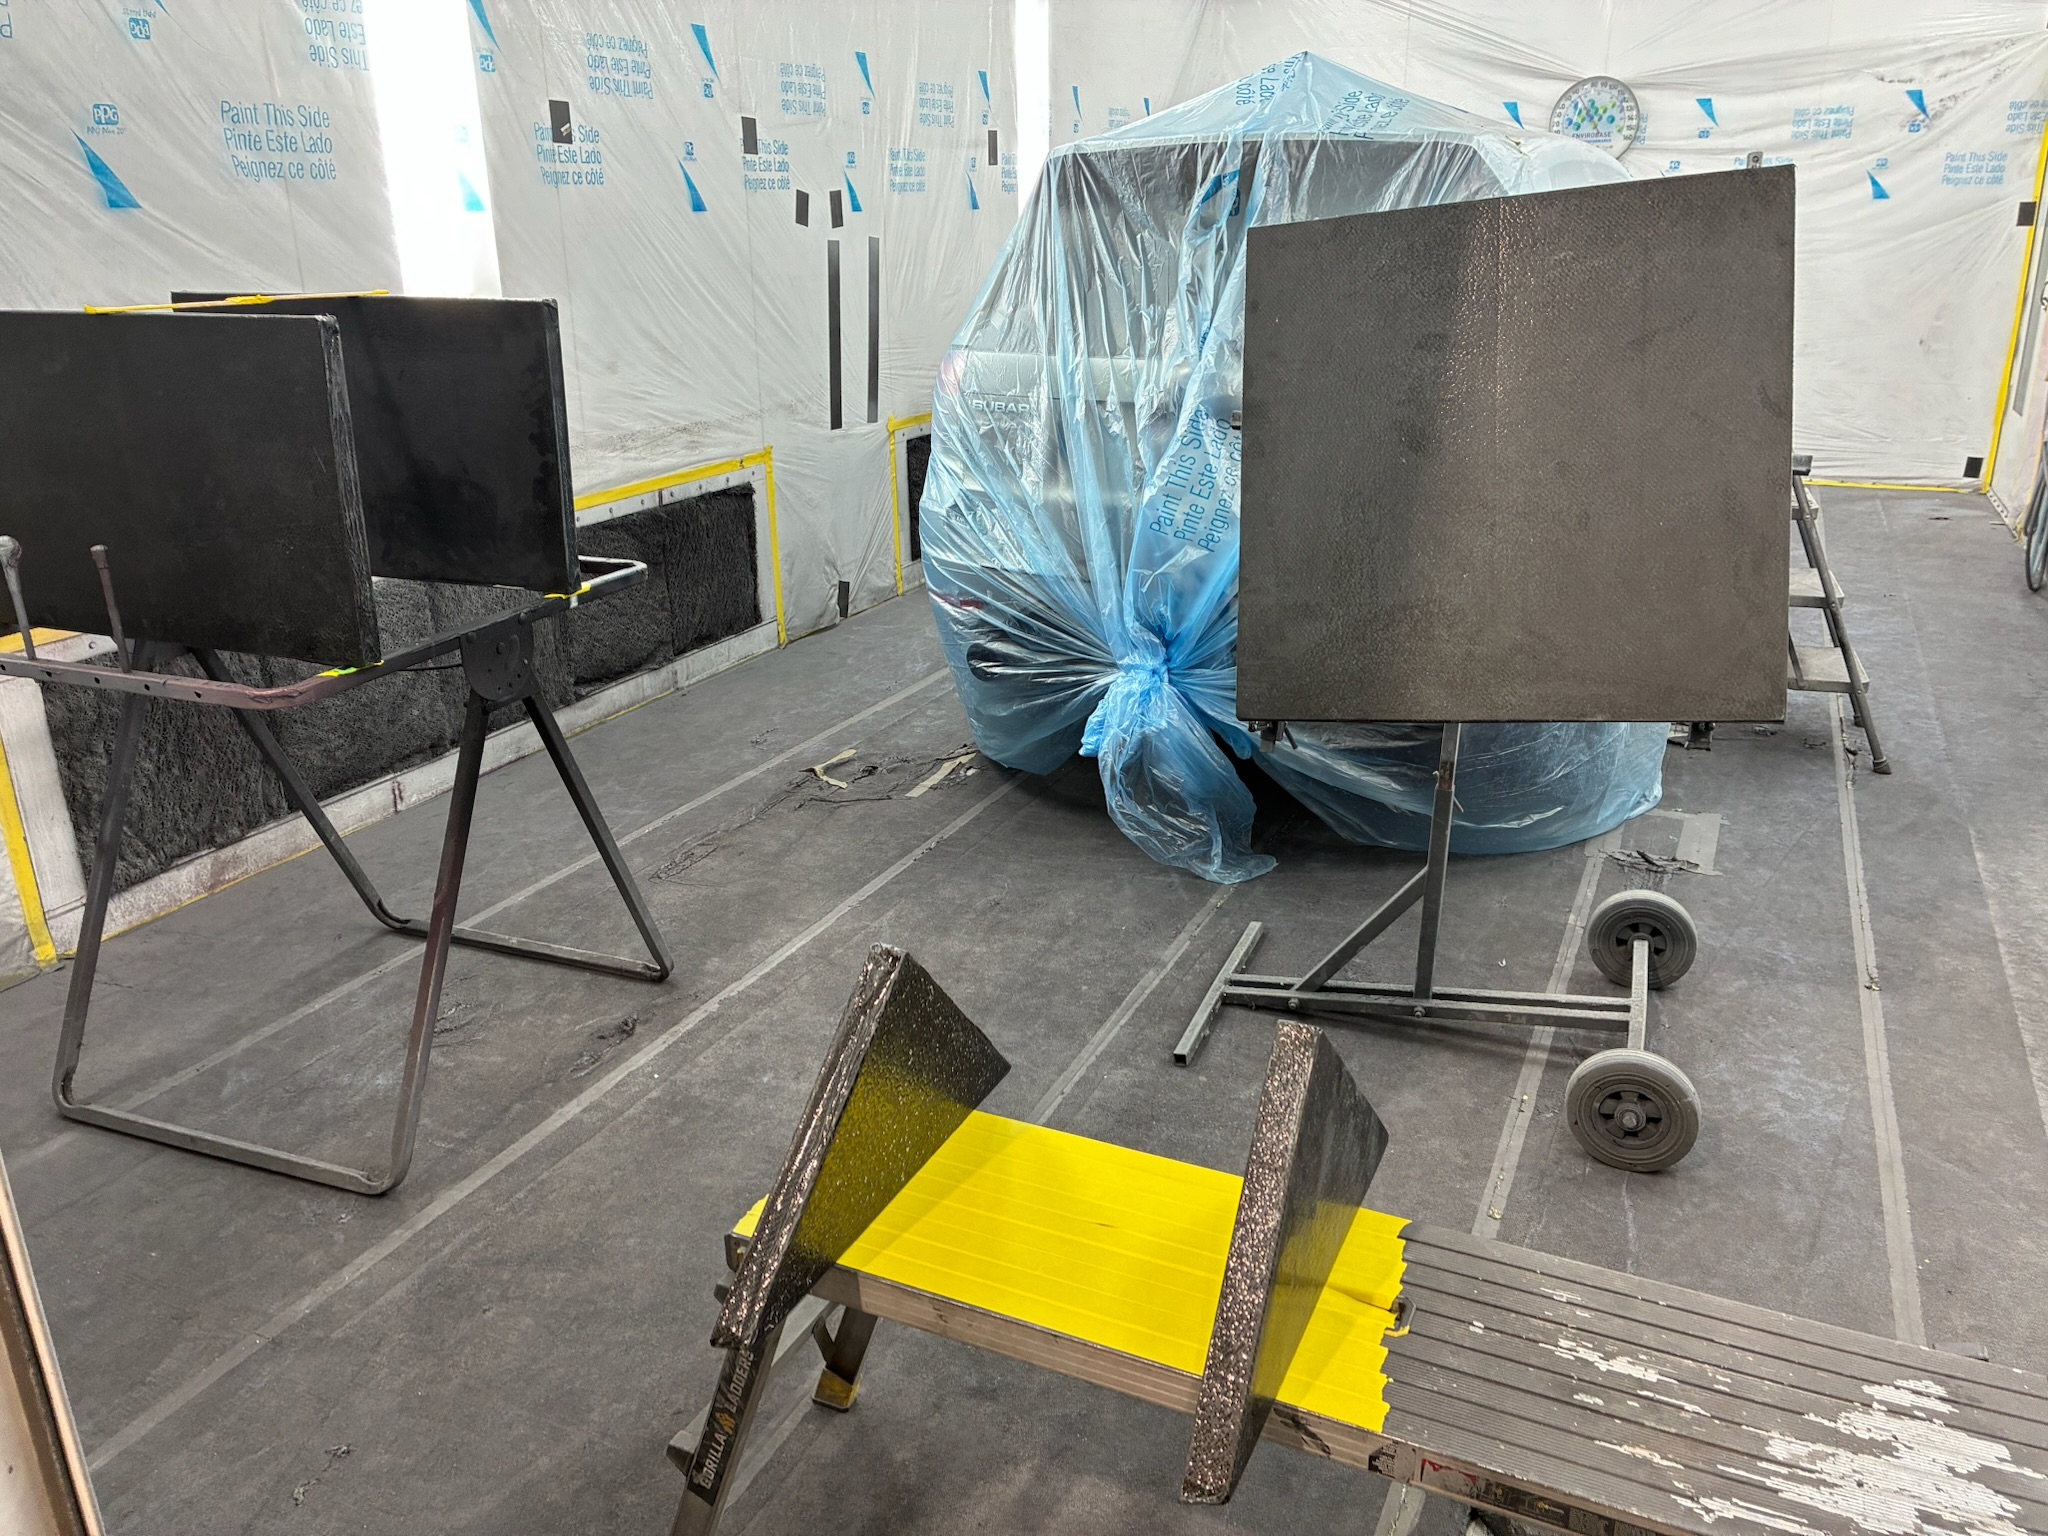
\includegraphics[
        width=2.35in,
        height=1.40in,
        keepaspectratio
    ]{topcoat_setup_apparatus}
};
\draw[RuleGray,line width=0.55pt,rounded corners=4pt]
    ($(current page.north west)+(5.77in,-1.91in)$)
    rectangle
    ($(current page.north west)+(8.32in,-3.40in)$);

% Image 4
\node[anchor=center,inner sep=0pt]
at ($(current page.north west)+(9.50in,-2.655in)$)
{
    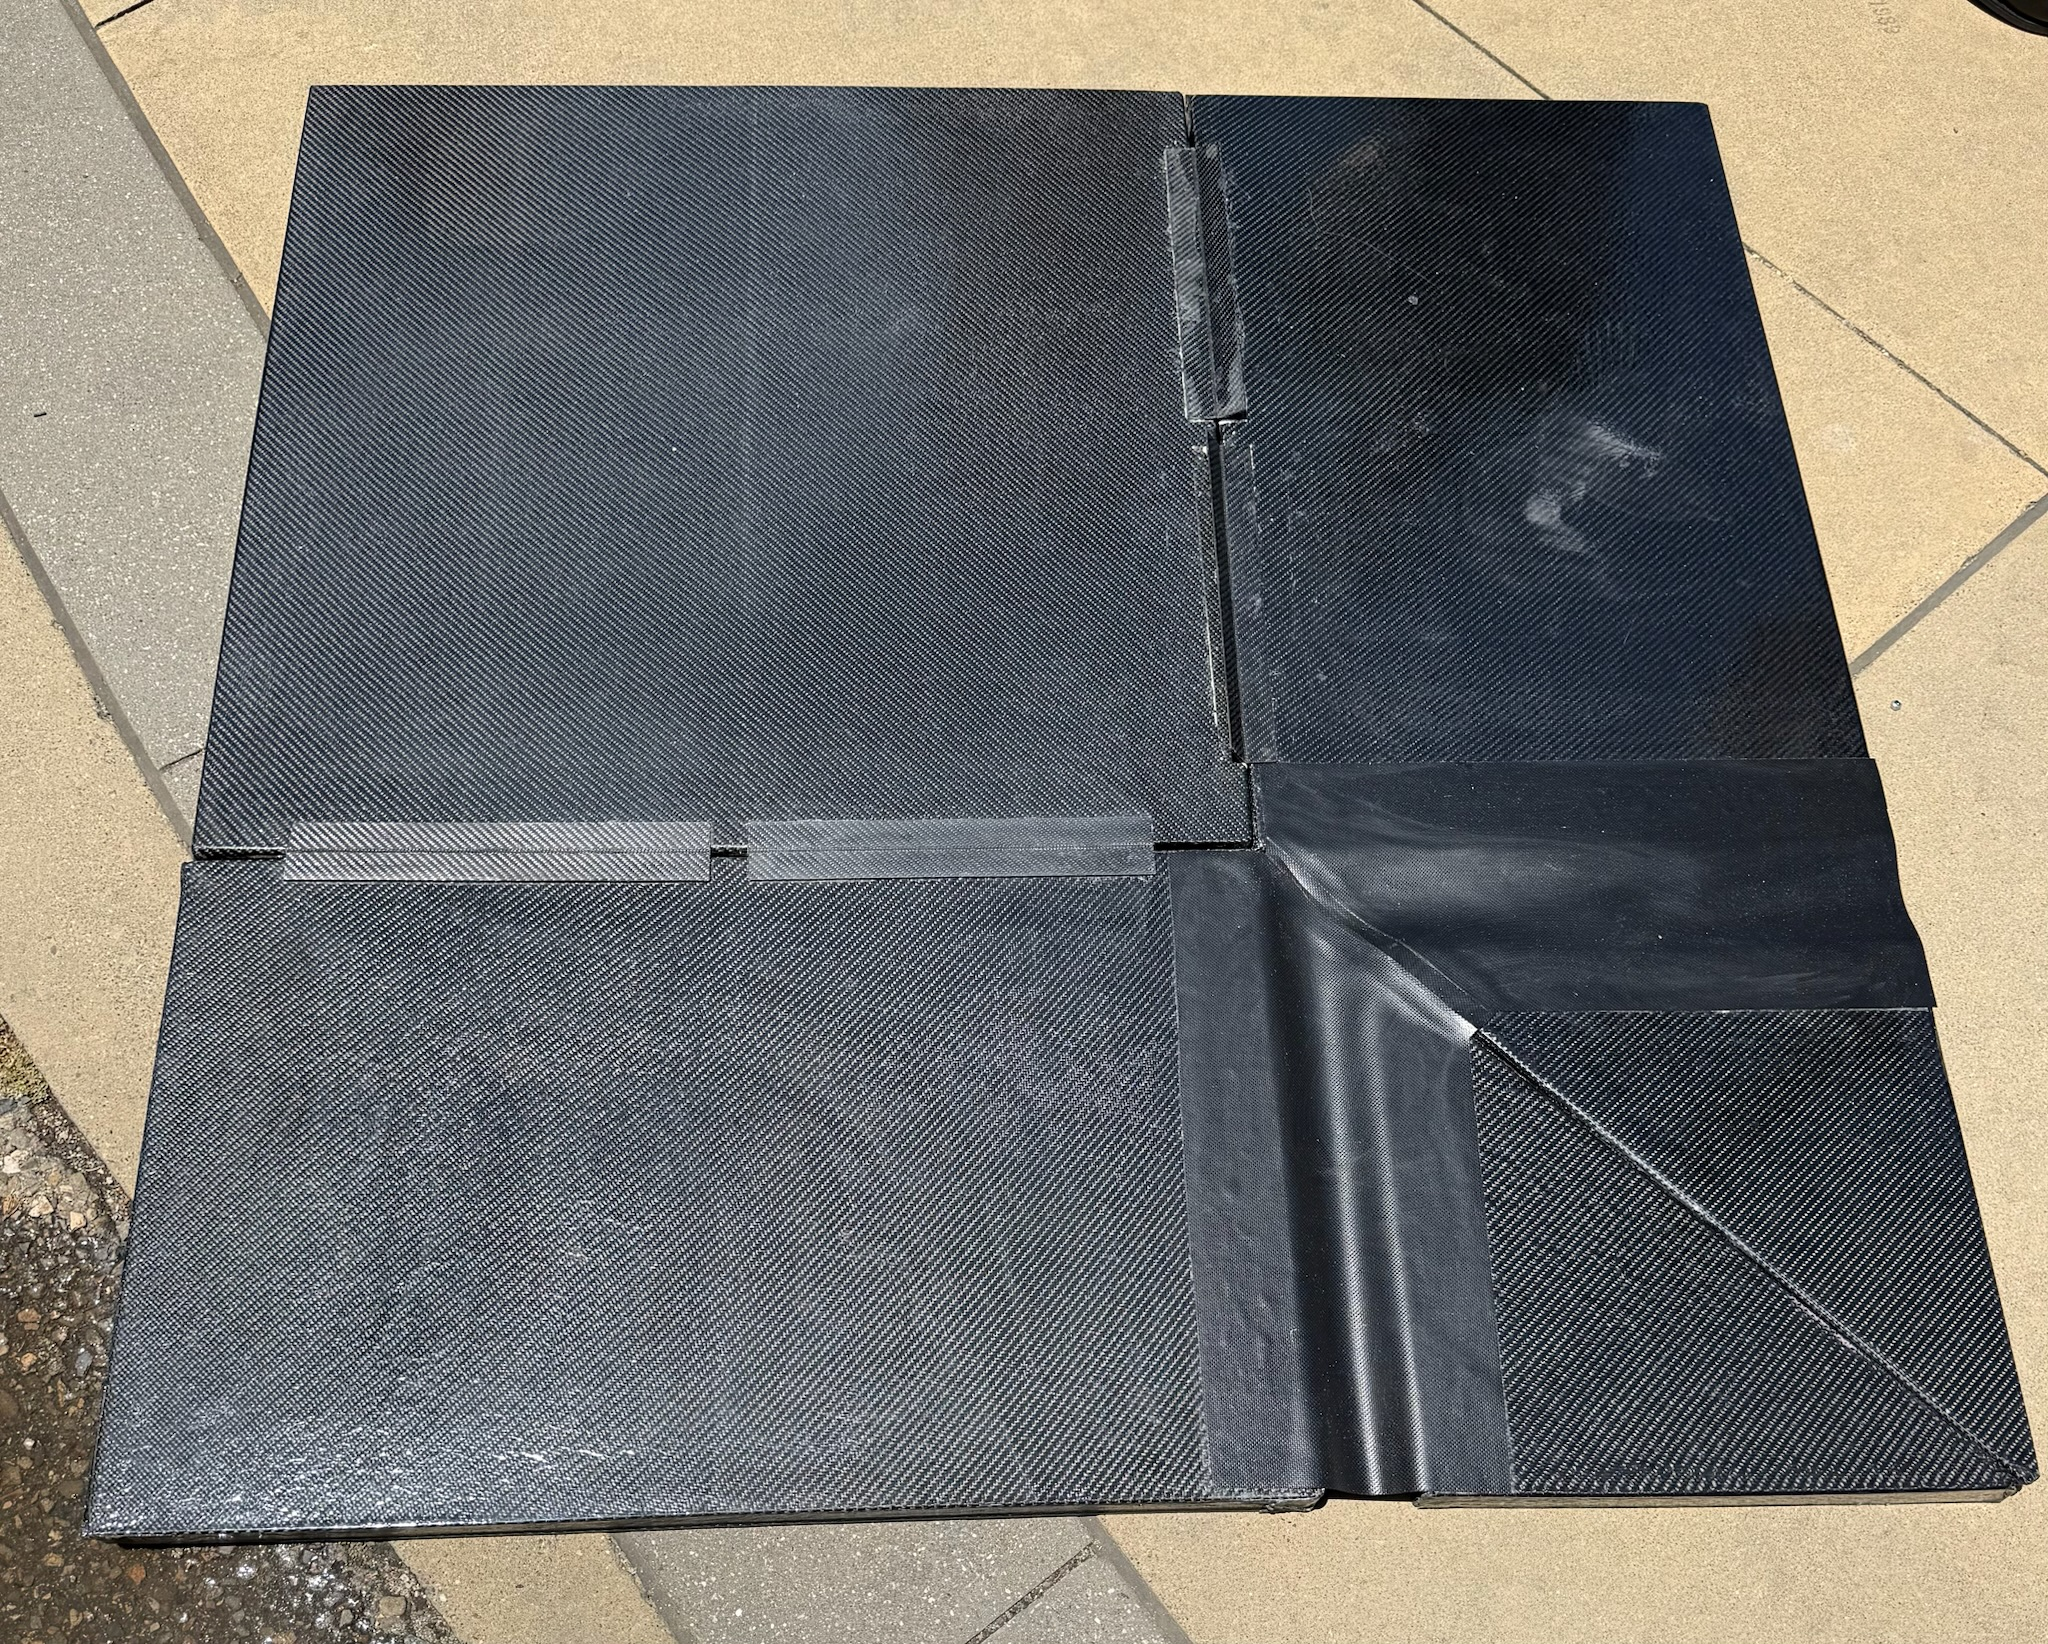
\includegraphics[
        width=2.35in,
        height=1.40in,
        keepaspectratio
    ]{refined_final_toro_cover_partial_carbon_model}
};
\draw[RuleGray,line width=0.55pt,rounded corners=4pt]
    ($(current page.north west)+(8.44in,-1.91in)$)
    rectangle
    ($(current page.north east)+(-0.42in,-3.40in)$);

% Captions
\node[anchor=north,text=Muted,font=\sffamily\fontsize{6.7}{7.3}\selectfont]
at ($(current page.north west)+(1.705in,-3.45in)$)
{Topcoat material preparation};

\node[anchor=north,text=Muted,font=\sffamily\fontsize{6.7}{7.3}\selectfont]
at ($(current page.north west)+(4.375in,-3.45in)$)
{Automotive-booth topcoat application};

\node[anchor=north,text=Muted,font=\sffamily\fontsize{6.7}{7.3}\selectfont]
at ($(current page.north west)+(7.045in,-3.45in)$)
{Coated panels drying after application};

\node[anchor=north,text=Muted,font=\sffamily\fontsize{6.7}{7.3}\selectfont]
at ($(current page.north west)+(9.50in,-3.45in)$)
{Partial carbon manufacturing model};

% Environmental rationale
\fill[SoftGold,rounded corners=4pt]
    ($(current page.north west)+(0.43in,-3.73in)$)
    rectangle
    ($(current page.north east)+(-0.42in,-4.76in)$);

\node[
    anchor=north west,
    align=left,
    text width=9.75in,
    text=Ink,
    font=\fontsize{7.05}{8.25}\selectfont
]
at ($(current page.north west)+(0.65in,-3.89in)$)
{
Because the sponsor required a carbon-fiber cover for outdoor use near chlorinated water,
environmental protection became a functional requirement rather than a cosmetic finish.
I selected and personally sprayed a UV-resistant Sunshield topcoat to seal minor laminate
porosity, reduce moisture ingress, preserve the carbon appearance, limit UV degradation of
the epoxy matrix, and isolate the composite surface from nearby metallic hardware.
};

% Results title
\node[
    anchor=north west,
    text=DeepGreen,
    font=\sffamily\bfseries\fontsize{8.0}{8.7}\selectfont
]
at ($(current page.north west)+(0.43in,-4.94in)$)
{FUNCTIONAL PROTOTYPE RESULTS};

% ------------------------------------------------------------
% Matched lower panels — larger type and improved allocation
% ------------------------------------------------------------

% Left results panel
\fill[SoftGreen,rounded corners=5pt]
    ($(current page.north west)+(0.43in,-5.22in)$)
    rectangle
    ($(current page.north west)+(5.98in,-7.39in)$);

\draw[RuleGray,line width=0.65pt,rounded corners=5pt]
    ($(current page.north west)+(0.43in,-5.22in)$)
    rectangle
    ($(current page.north west)+(5.98in,-7.39in)$);

\fill[DeepGreen,rounded corners=5pt]
    ($(current page.north west)+(0.43in,-5.22in)$)
    rectangle
    ($(current page.north west)+(5.98in,-5.58in)$);

\fill[DeepGreen]
    ($(current page.north west)+(0.43in,-5.40in)$)
    rectangle
    ($(current page.north west)+(5.98in,-5.58in)$);

\node[anchor=west,text=white,
      font=\sffamily\bfseries\fontsize{7.0}{7.6}\selectfont]
at ($(current page.north west)+(0.66in,-5.40in)$)
{SPECIFICATION};

\node[anchor=west,text=white,
      font=\sffamily\bfseries\fontsize{7.0}{7.6}\selectfont]
at ($(current page.north west)+(3.02in,-5.40in)$)
{RESULT};

\node[anchor=east,text=white,
      font=\sffamily\bfseries\fontsize{7.0}{7.6}\selectfont]
at ($(current page.north west)+(5.55in,-5.40in)$)
{STATUS};

\node[
    anchor=north west,
    align=left,
    text width=2.15in,
    text=Ink,
    font=\bfseries\fontsize{7.15}{8.55}\selectfont
]
at ($(current page.north west)+(0.66in,-5.72in)$)
{
Deployment time\\[3.4pt]
Removal time\\[3.4pt]
Single-user operation\\[3.4pt]
Single-side operation\\[3.4pt]
Deployment steps\\[3.4pt]
Removal steps\\[3.4pt]
Weight\\[3.4pt]
Folded storage
};

\node[
    anchor=north west,
    align=left,
    text width=1.45in,
    text=Ink,
    font=\fontsize{7.15}{8.55}\selectfont
]
at ($(current page.north west)+(3.02in,-5.72in)$)
{
25.51 seconds\\[3.4pt]
37.22 seconds\\[3.4pt]
100\% successful\\[3.4pt]
75\% successful\\[3.4pt]
6.4 average\\[3.4pt]
9 average\\[3.4pt]
17 lb\\[3.4pt]
2.9' x 2.9' x 1.7'
};

\node[
    anchor=north east,
    align=right,
    text width=1.05in,
    text=DeepGreen,
    font=\sffamily\bfseries\fontsize{7.05}{8.55}\selectfont
]
at ($(current page.north west)+(5.55in,-5.72in)$)
{
PASS\\[3.4pt]
PASS\\[3.4pt]
PASS\\[3.4pt]
NEAR TARGET\\[3.4pt]
PASS\\[3.4pt]
PASS\\[3.4pt]
NEAR TARGET\\[3.4pt]
PASS
};

% Right takeaways panel — widened for easier reading
\fill[SoftGreen,rounded corners=5pt]
    ($(current page.north west)+(6.14in,-5.22in)$)
    rectangle
    ($(current page.north east)+(-0.42in,-7.39in)$);

\draw[RuleGray,line width=0.65pt,rounded corners=5pt]
    ($(current page.north west)+(6.14in,-5.22in)$)
    rectangle
    ($(current page.north east)+(-0.42in,-7.39in)$);

\fill[DeepGreen,rounded corners=5pt]
    ($(current page.north west)+(6.14in,-5.22in)$)
    rectangle
    ($(current page.north east)+(-0.42in,-5.58in)$);

\fill[DeepGreen]
    ($(current page.north west)+(6.14in,-5.40in)$)
    rectangle
    ($(current page.north east)+(-0.42in,-5.58in)$);

\node[anchor=west,text=white,
      font=\sffamily\bfseries\fontsize{7.1}{7.7}\selectfont]
at ($(current page.north west)+(6.38in,-5.40in)$)
{ENGINEERING TAKEAWAYS};

\node[
    anchor=north west,
    align=left,
    text width=4.02in,
    text=Ink,
    font=\fontsize{6.75}{7.85}\selectfont
]
at ($(current page.north west)+(6.38in,-5.72in)$)
{
\textbf{Manufacturing first.}
Composite manufacturing constraints should guide the product architecture from the beginning.\\[4.5pt]
\textbf{Prioritize deliberately.}
Competing requirements must be balanced intentionally instead of maximizing every objective.\\[4.5pt]
\textbf{Lead through the process.}
Clear procedures, calm communication, and respect for teammates' strengths were essential during fabrication.\\[4.5pt]
\textbf{Next iteration.}
Reduce weight, refine the fabric-hinge fold lines, and improve panel-edge clearance.
};

% Compact concluding pathway
\node[
    anchor=center,
    align=center,
    text=PolyGold,
    font=\sffamily\bfseries\fontsize{6.3}{6.9}\selectfont
]
at ($(current page.north)+(3.06in,-7.18in)$)
{PROTOTYPE \faArrowRight\ DESIGN REFINEMENT
\faArrowRight\ REPEATABLE MANUFACTURING
\faArrowRight\ PRODUCT};

% Validation resources
\node[
    anchor=north,
    align=center,
    text=DeepGreen,
    font=\sffamily\bfseries\fontsize{6.6}{7.2}\selectfont
]
at ($(current page.north)+(0,-7.58in)$)
{\href{\ToroDeploymentLink}{\faPlayCircle\ DEPLOYMENT}
\hspace{18pt}
\href{\ToroRemovalLink}{\faPlayCircle\ REMOVAL / FOLDING}
\hspace{18pt}
\href{\ToroPosterLink}{\faFilePdf\ EXPO POSTER}
\hspace{18pt}
\href{\ToroReportLink}{\faFilePdf\ FINAL REPORT}};

% Footer
\node[
    anchor=south west,
    text=white,
    font=\sffamily\bfseries\fontsize{7.1}{7.7}\selectfont
]
at ($(current page.south west)+(0.42in,0.17in)$)
{\faArrowLeft\ MANUFACTURING-DRIVEN DESIGN};

\node[
    anchor=south,
    text=white,
    font=\sffamily\fontsize{7.0}{7.6}\selectfont
]
at ($(current page.south)+(0,0.17in)$)
{TORO COVER \hspace{6pt} 3 / 3};

\node[
    anchor=south east,
    text=white,
    font=\sffamily\bfseries\fontsize{7.1}{7.7}\selectfont
]
at ($(current page.south east)+(-0.42in,0.17in)$)
{NEXT PROJECT \faArrowRight};

\end{tikzpicture}

% ============================================================
% PICKLEBALL PADDLE — SINGLE-PAGE PORTFOLIO CASE STUDY
% Project 02 in the Composites section
%
% IMPORTANT:
% 1. This file must NOT contain \documentclass, \begin{document},
%    or \end{document}.
% 2. In main.tex, place \input{pickleball} before \end{document}.
% 3. Image references use these Overleaf base filenames:
%       waterjet
%       side_core_view
%       full_assy
%       front_view
%       LAMINATE
% ============================================================

% Clickable project resource
\providecommand{\PaddleWaterjetVideo}
{https://drive.google.com/file/d/1mTuaE_g5mE2f7Nn3R5k7yFxqCWH_pvBh/view?usp=drive_link}

\clearpage
\thispagestyle{empty}
\hypertarget{pickleball}{}
\null

\begin{tikzpicture}[remember picture,overlay]

% ============================================================
% BACKGROUND AND PAGE BARS
% ============================================================

\fill[white]
    (current page.south west)
    rectangle
    (current page.north east);

\fill[DeepGreen]
    (current page.north west)
    rectangle
    ($(current page.north east)+(0,-0.095in)$);

\fill[PolyGold]
    ($(current page.north west)+(0,-0.095in)$)
    rectangle
    ($(current page.north east)+(0,-0.14in)$);

\fill[DeepGreen]
    (current page.south west)
    rectangle
    ($(current page.south east)+(0,0.36in)$);

\fill[PolyGold]
    ($(current page.south west)+(0,0.36in)$)
    rectangle
    ($(current page.south east)+(0,0.405in)$);

% ============================================================
% HEADER
% ============================================================

\node[
    anchor=north west,
    text=PolyGold,
    font=\sffamily\bfseries\fontsize{8.1}{8.7}\selectfont
]
at ($(current page.north west)+(0.42in,-0.39in)$)
{01 COMPOSITES \hspace{5pt}/\hspace{5pt} PROJECT 02};

\node[
    anchor=north west,
    text=DeepGreen,
    font=\bfseries\fontsize{22.5}{23.5}\selectfont
]
at ($(current page.north west)+(0.40in,-0.67in)$)
{CARBON FIBER PICKLEBALL PADDLE};

\node[
    anchor=north west,
    text=Muted,
    font=\sffamily\fontsize{8.4}{9.2}\selectfont
]
at ($(current page.north west)+(0.42in,-1.12in)$)
{Cal Poly Composites Laboratory \hspace{7pt}\textbullet\hspace{7pt}
Individual Project \hspace{7pt}\textbullet\hspace{7pt}
Spring 2026 \hspace{7pt}\textbullet\hspace{7pt}
San Luis Obispo, California};

\fill[PolyGold]
    ($(current page.north west)+(0.42in,-1.36in)$)
    rectangle
    ($(current page.north west)+(6.10in,-1.315in)$);

% ============================================================
% TOP LEFT — HERO PRODUCT IMAGE
% ============================================================

\node[
    anchor=center,
    inner sep=3pt,
    draw=DeepGreen,
    line width=0.75pt,
    rounded corners=6pt
]
at ($(current page.north west)+(1.60in,-3.20in)$)
{
    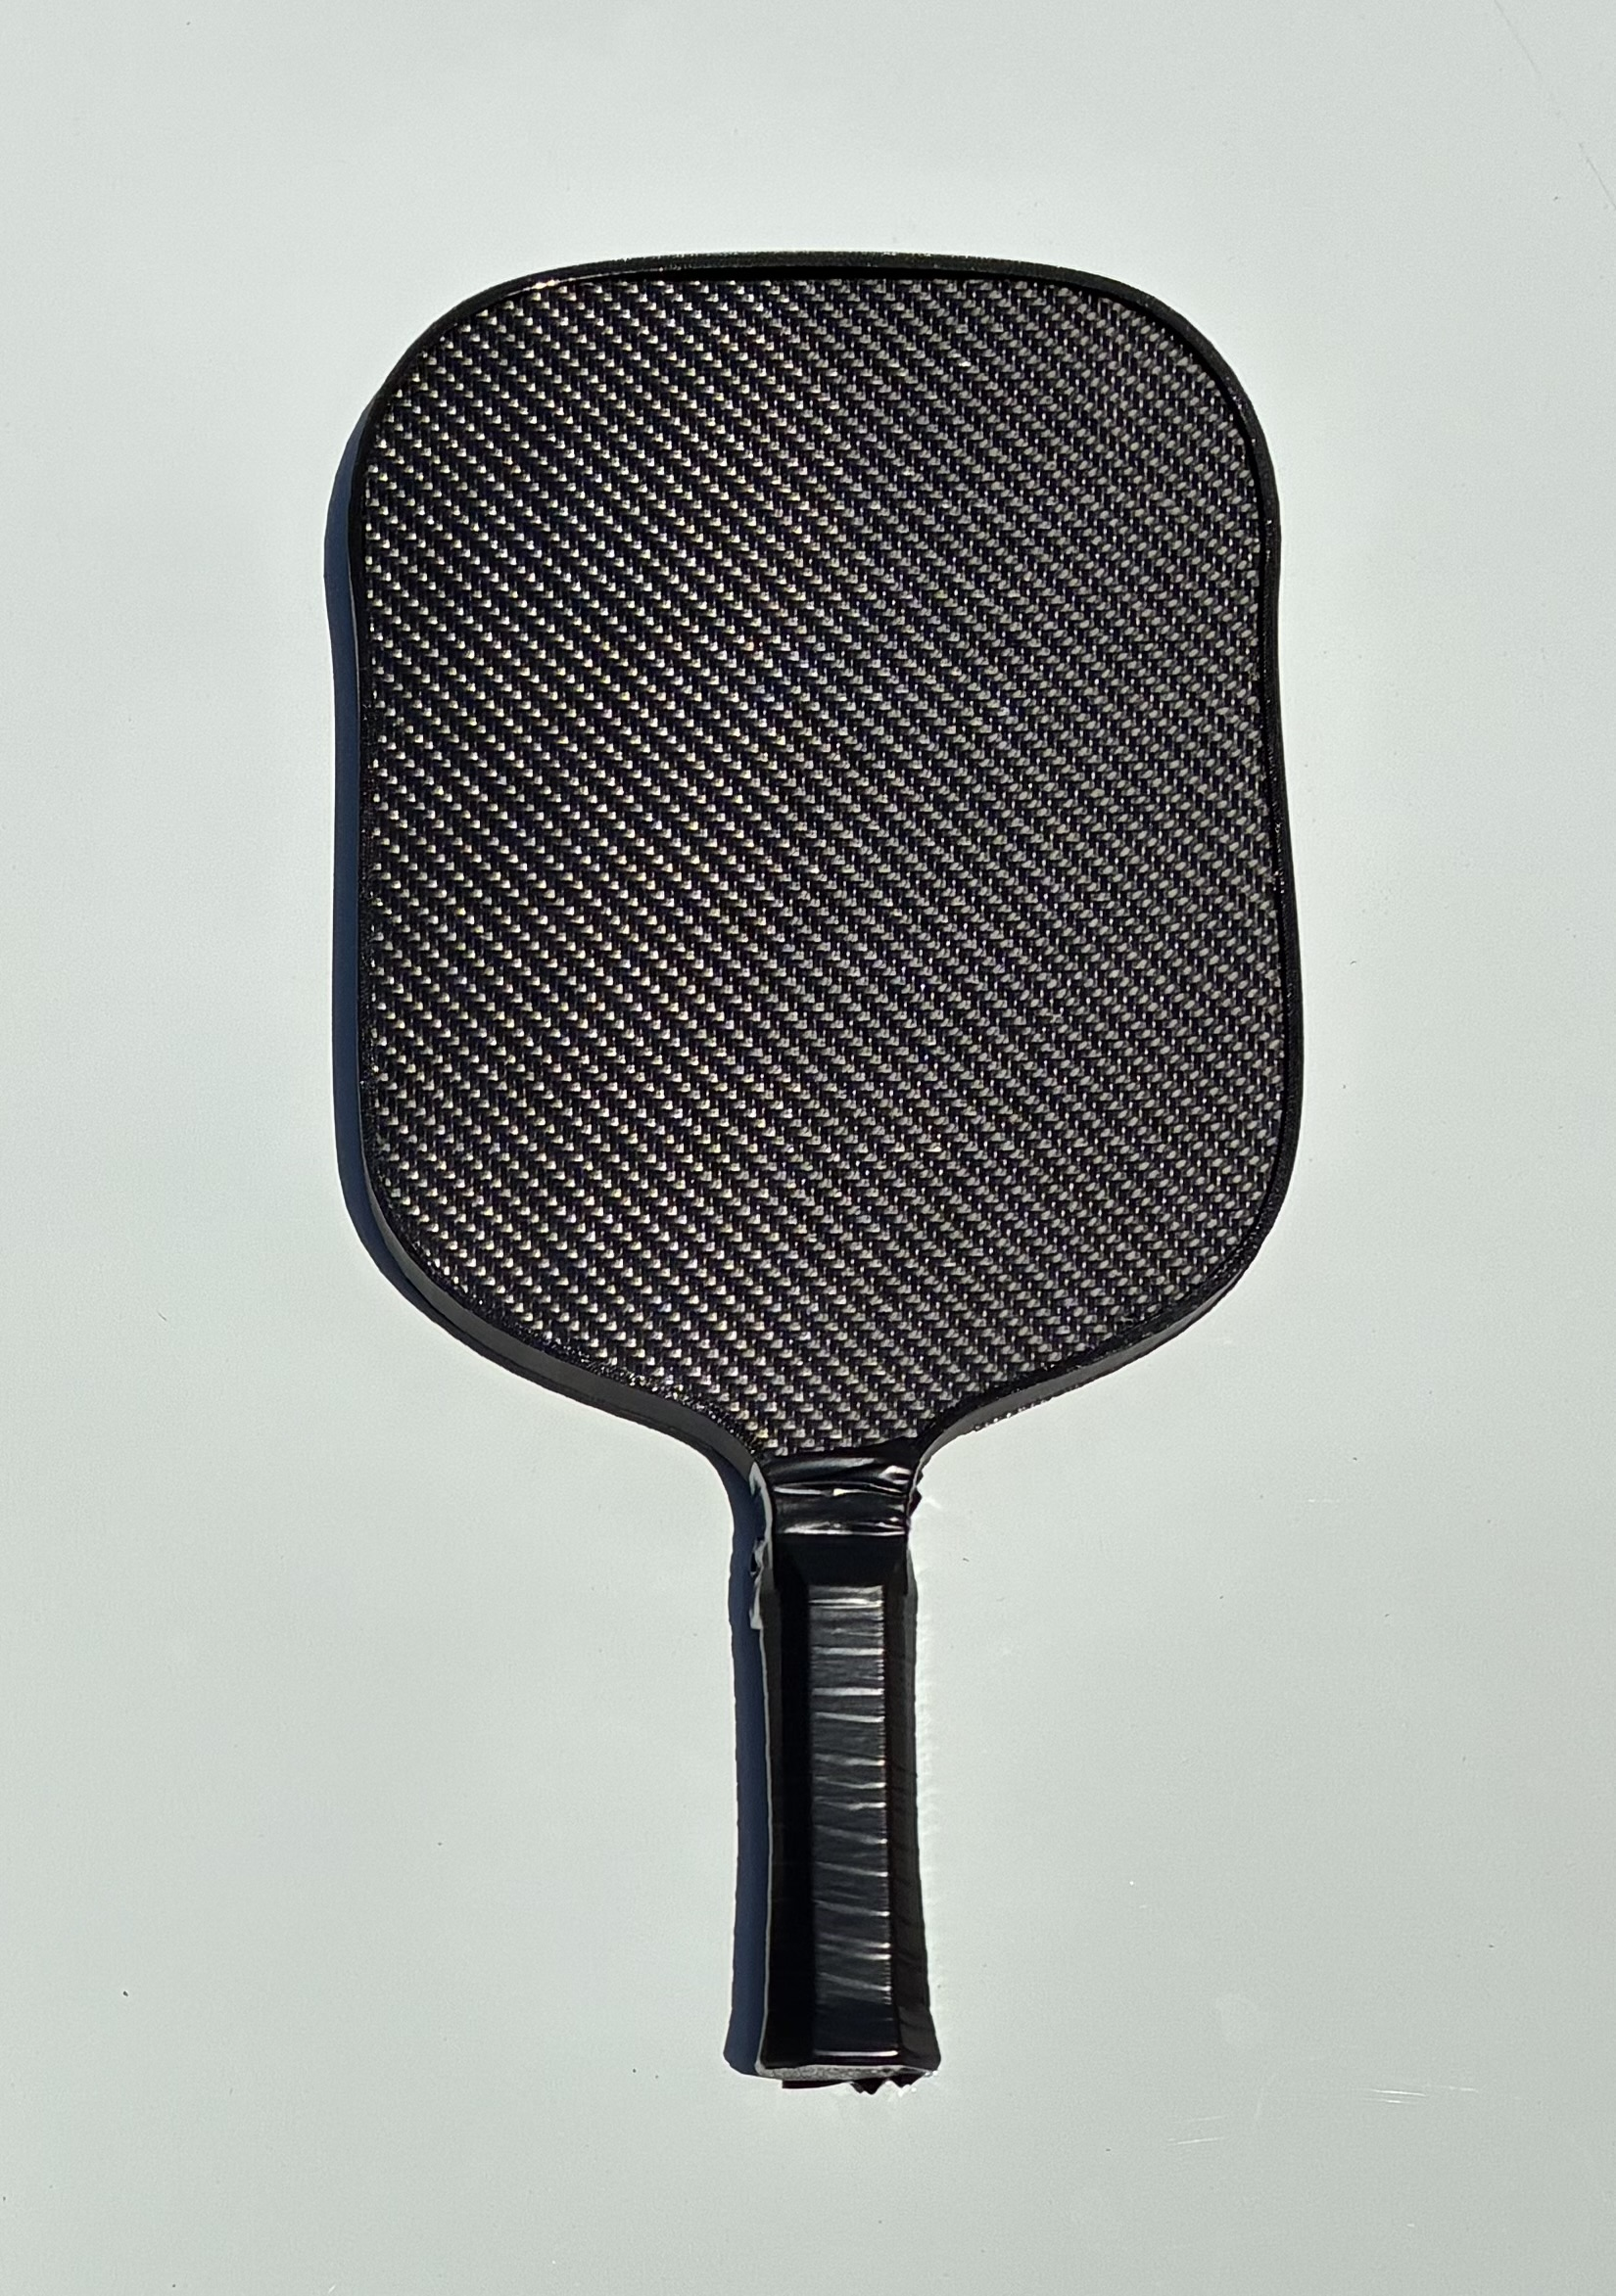
\includegraphics[
        width=3.72in,
        height=3.18in,
        keepaspectratio
    ]{full_assy}
};

\node[
    anchor=north,
    text=Muted,
    font=\sffamily\fontsize{6.9}{7.5}\selectfont
]
at ($(current page.north west)+(1.60in,-4.86in)$)
{Completed solo-built paddle assembly};

% ============================================================
% TOP CENTER — PROJECT OVERVIEW
% ============================================================

\fill[SoftGold,rounded corners=5pt]
    ($(current page.north west)+(2.95in,-1.62in)$)
    rectangle
    ($(current page.north west)+(5.53in,-4.86in)$);

\fill[PolyGold]
    ($(current page.north west)+(2.95in,-1.62in)$)
    rectangle
    ($(current page.north west)+(3.05in,-4.86in)$);

\node[
    anchor=north west,
    text=DeepGreen,
    font=\sffamily\bfseries\fontsize{8.0}{8.7}\selectfont
]
at ($(current page.north west)+(3.23in,-1.79in)$)
{PROJECT OVERVIEW};

\node[
    anchor=north west,
    align=left,
    text width=2.02in,
    text=Ink,
    font=\fontsize{7.05}{8.35}\selectfont
]
at ($(current page.north west)+(3.23in,-2.07in)$)
{
Independently designed and manufactured a lightweight prepreg
carbon-fiber pickleball paddle using a half-inch honeycomb
sandwich core, vacuum-bag consolidation, precision waterjet
trimming, and custom TPU and PLA components.

\vspace{5pt}

The project emphasized lightweight sandwich-composite design, repeatable manufacturing methods, dimensional accuracy, and the integration of custom 3D-printed TPU and PLA components into the final assembly.
};

\node[
    anchor=south west,
    align=left,
    text width=2.02in,
    text=PolyGold,
    font=\sffamily\bfseries\fontsize{6.65}{7.35}\selectfont
]
at ($(current page.north west)+(3.23in,-4.74in)$)
{
SOLE DESIGNER\\[2pt]
COMPOSITE FABRICATOR\\[2pt]
MANUFACTURING ENGINEER
};

% ============================================================
% TOP RIGHT — LAMINATE GRAPHIC
% ============================================================

\node[
    anchor=north west,
    inner sep=2.5pt,
    draw=DeepGreen,
    line width=0.65pt,
    rounded corners=5pt
]
at ($(current page.north west)+(5.71in,-1.62in)$)
{
    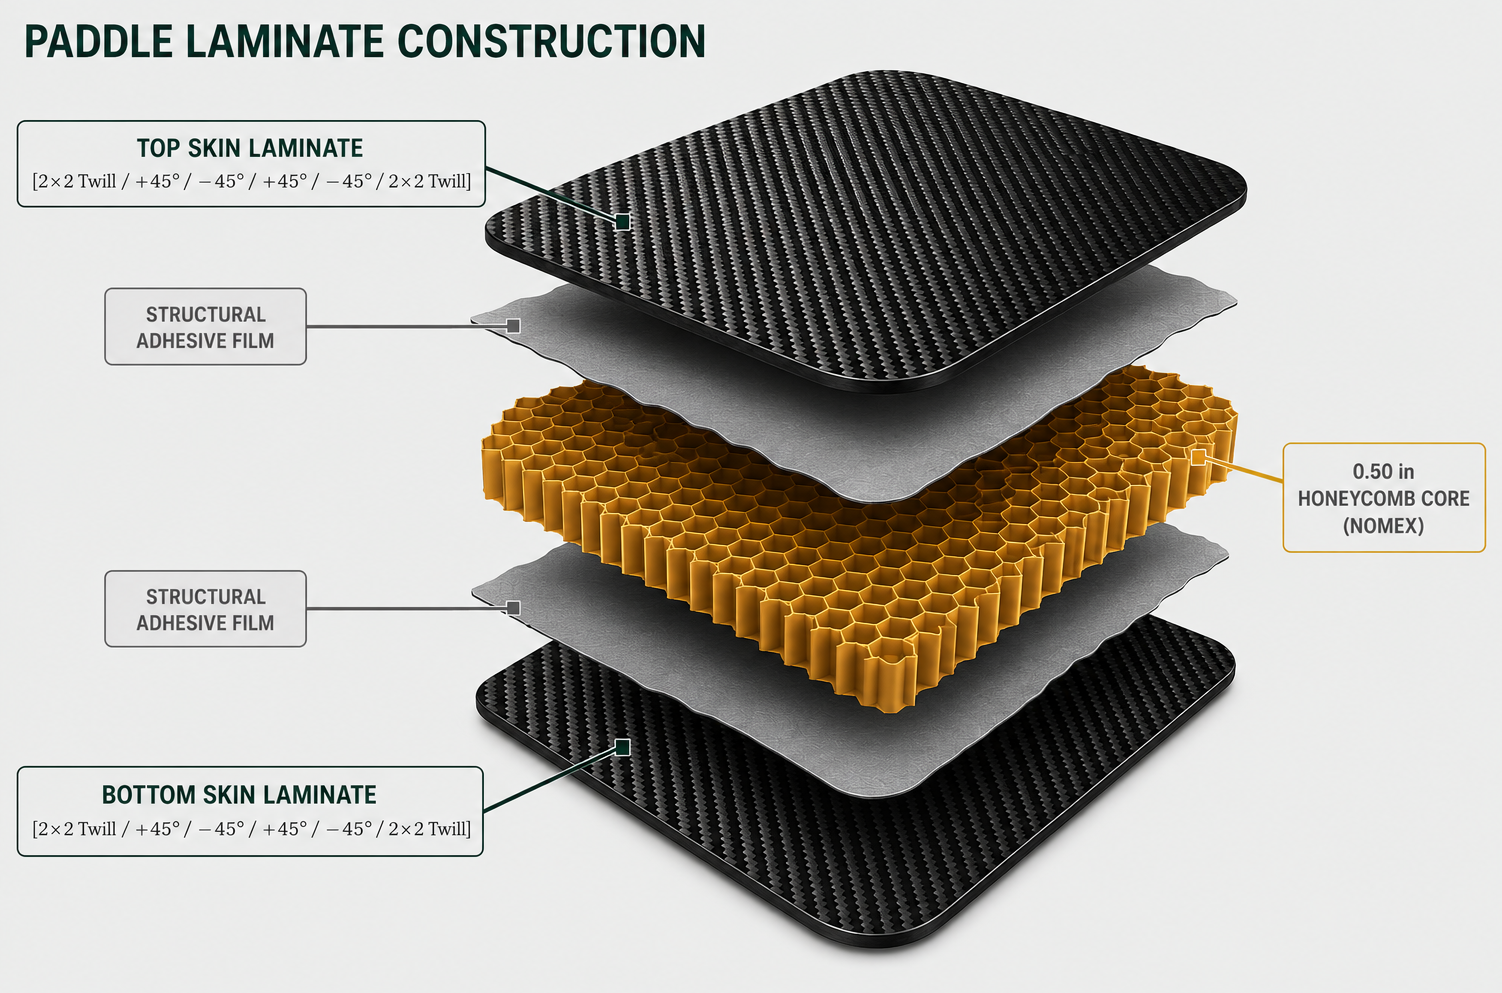
\includegraphics[
        width=4.80in,
        keepaspectratio
    ]{LAMINATE}
};

% ============================================================
% BOTTOM LEFT — SUPPORTING IMAGES
% ============================================================

\node[
    anchor=center,
    inner sep=3pt,
    draw=RuleGray,
    line width=0.55pt,
    rounded corners=4pt
]
at ($(current page.north west)+(1.12in,-5.98in)$)
{
    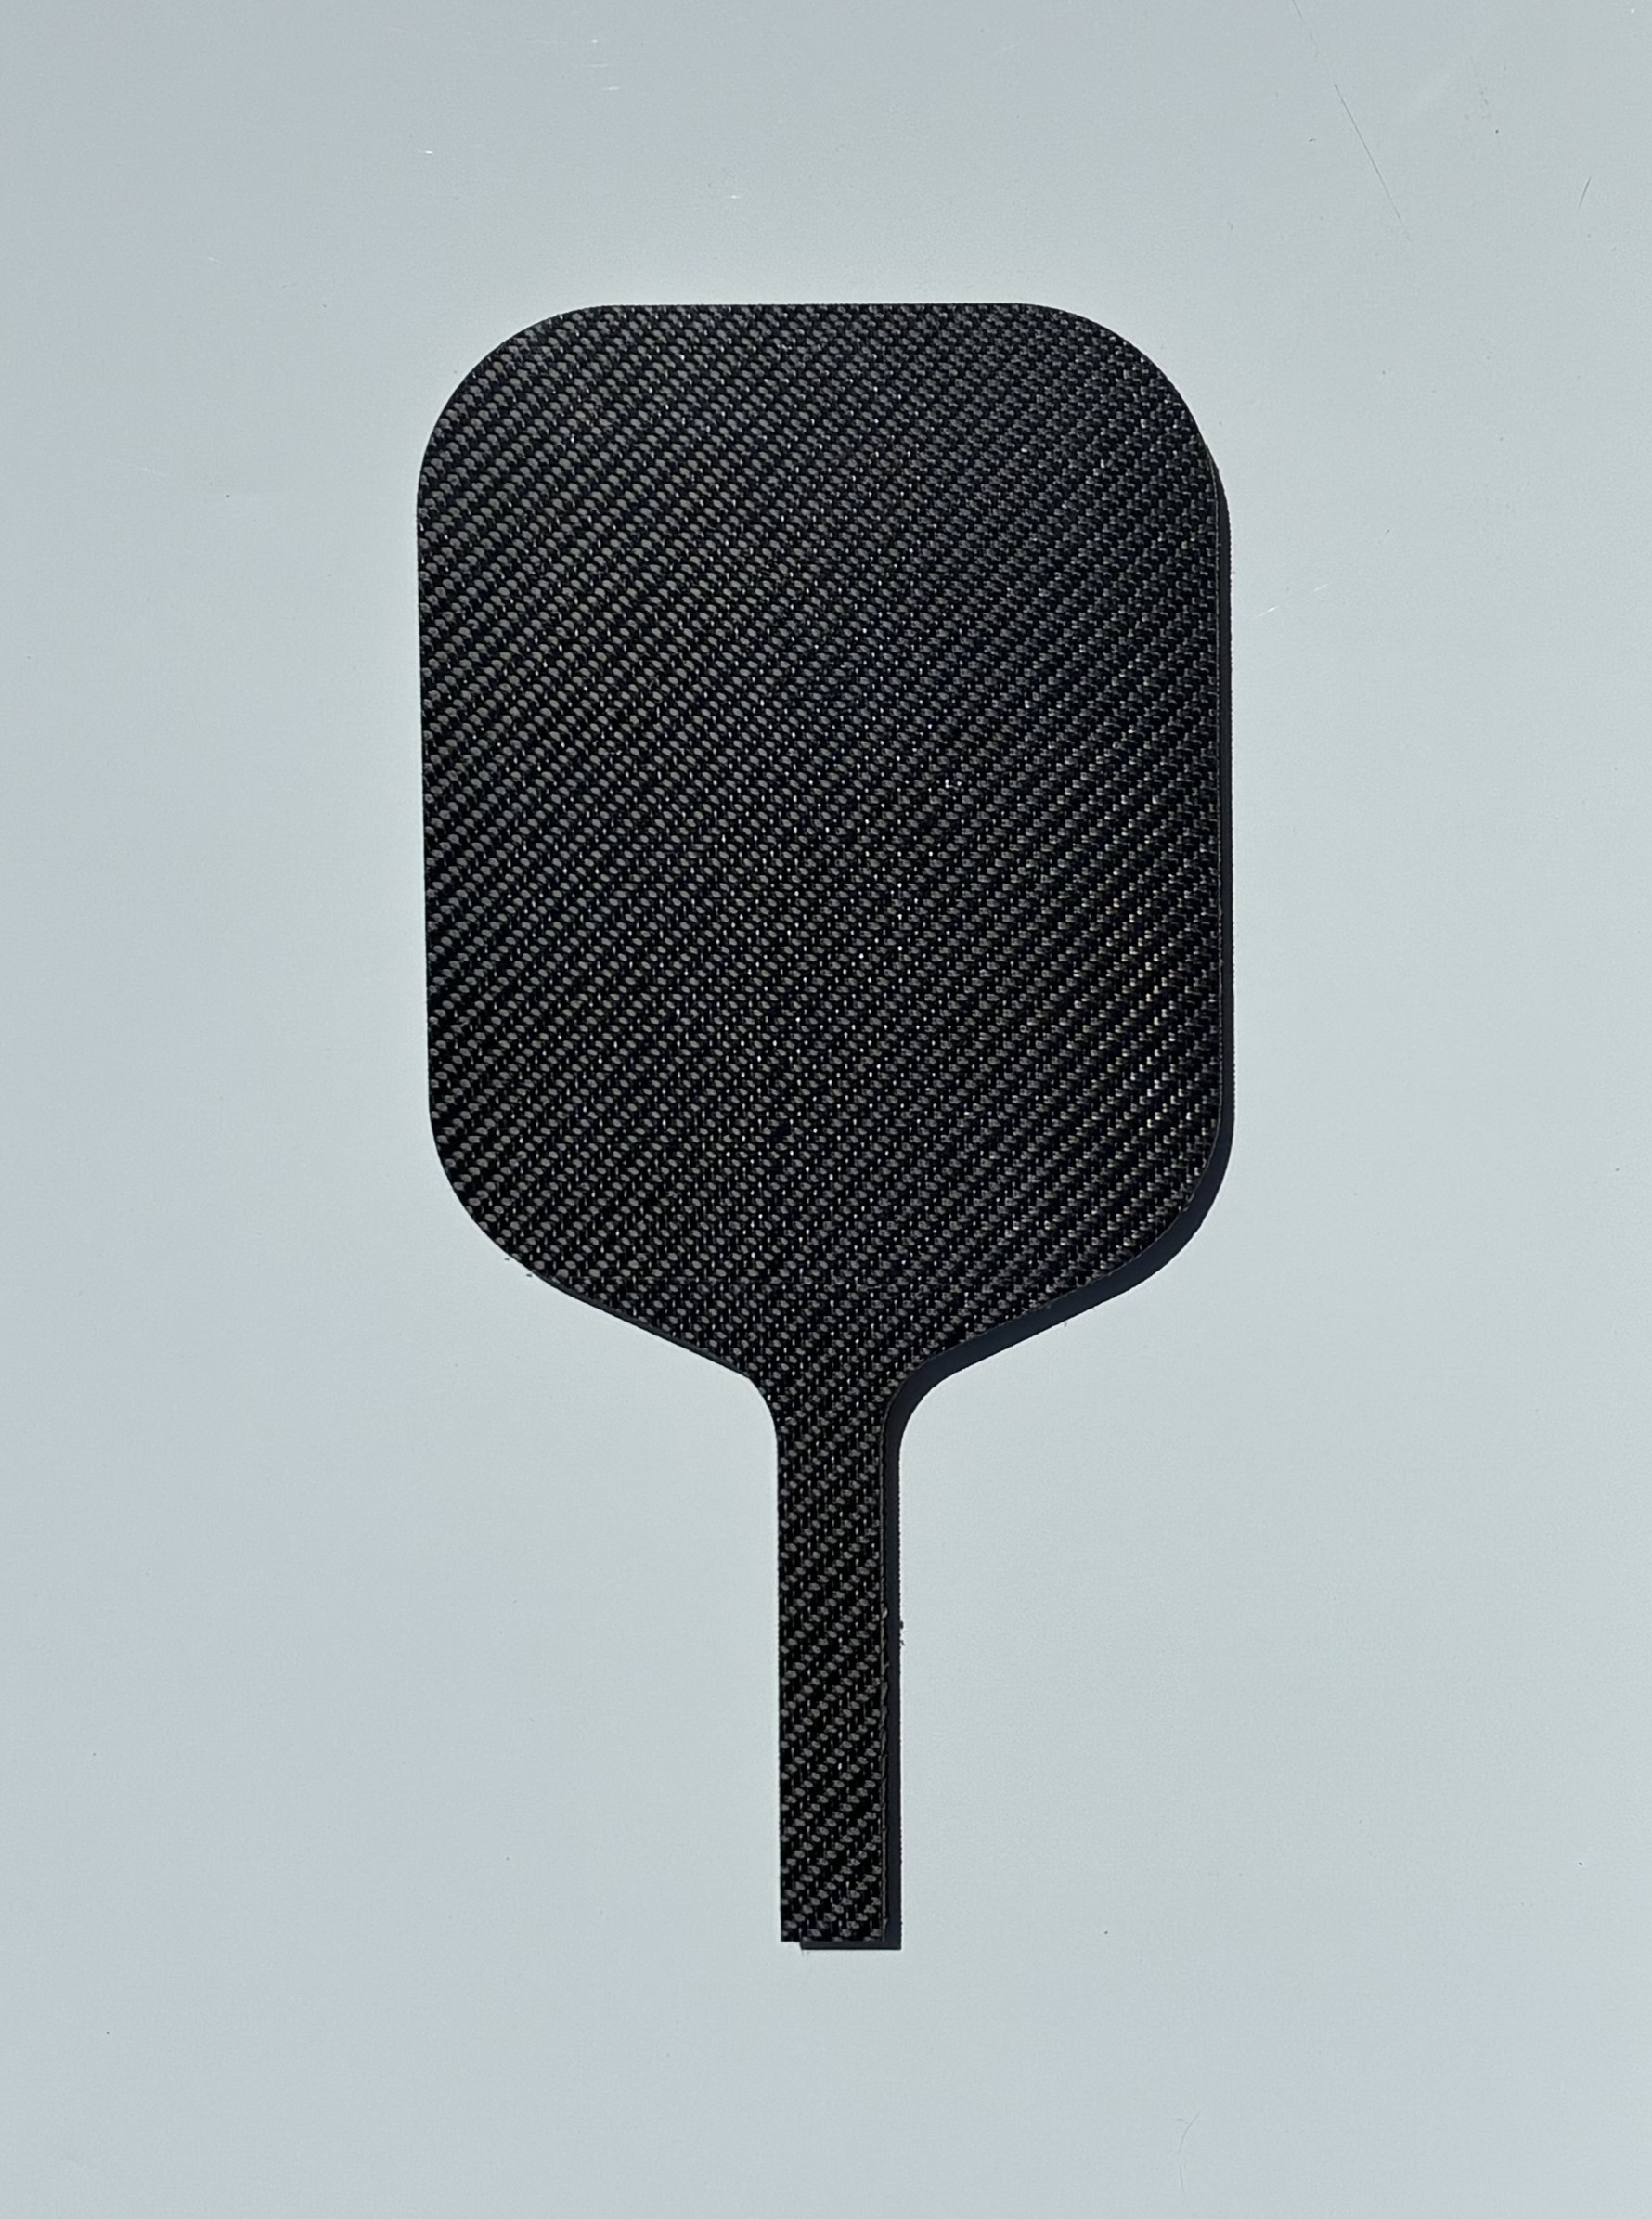
\includegraphics[
        width=1.30in,
        height=1.78in,
        keepaspectratio
    ]{front_view}
};

\node[
    anchor=center,
    inner sep=3pt,
    draw=RuleGray,
    line width=0.55pt,
    rounded corners=4pt
]
at ($(current page.north west)+(2.72in,-5.98in)$)
{
    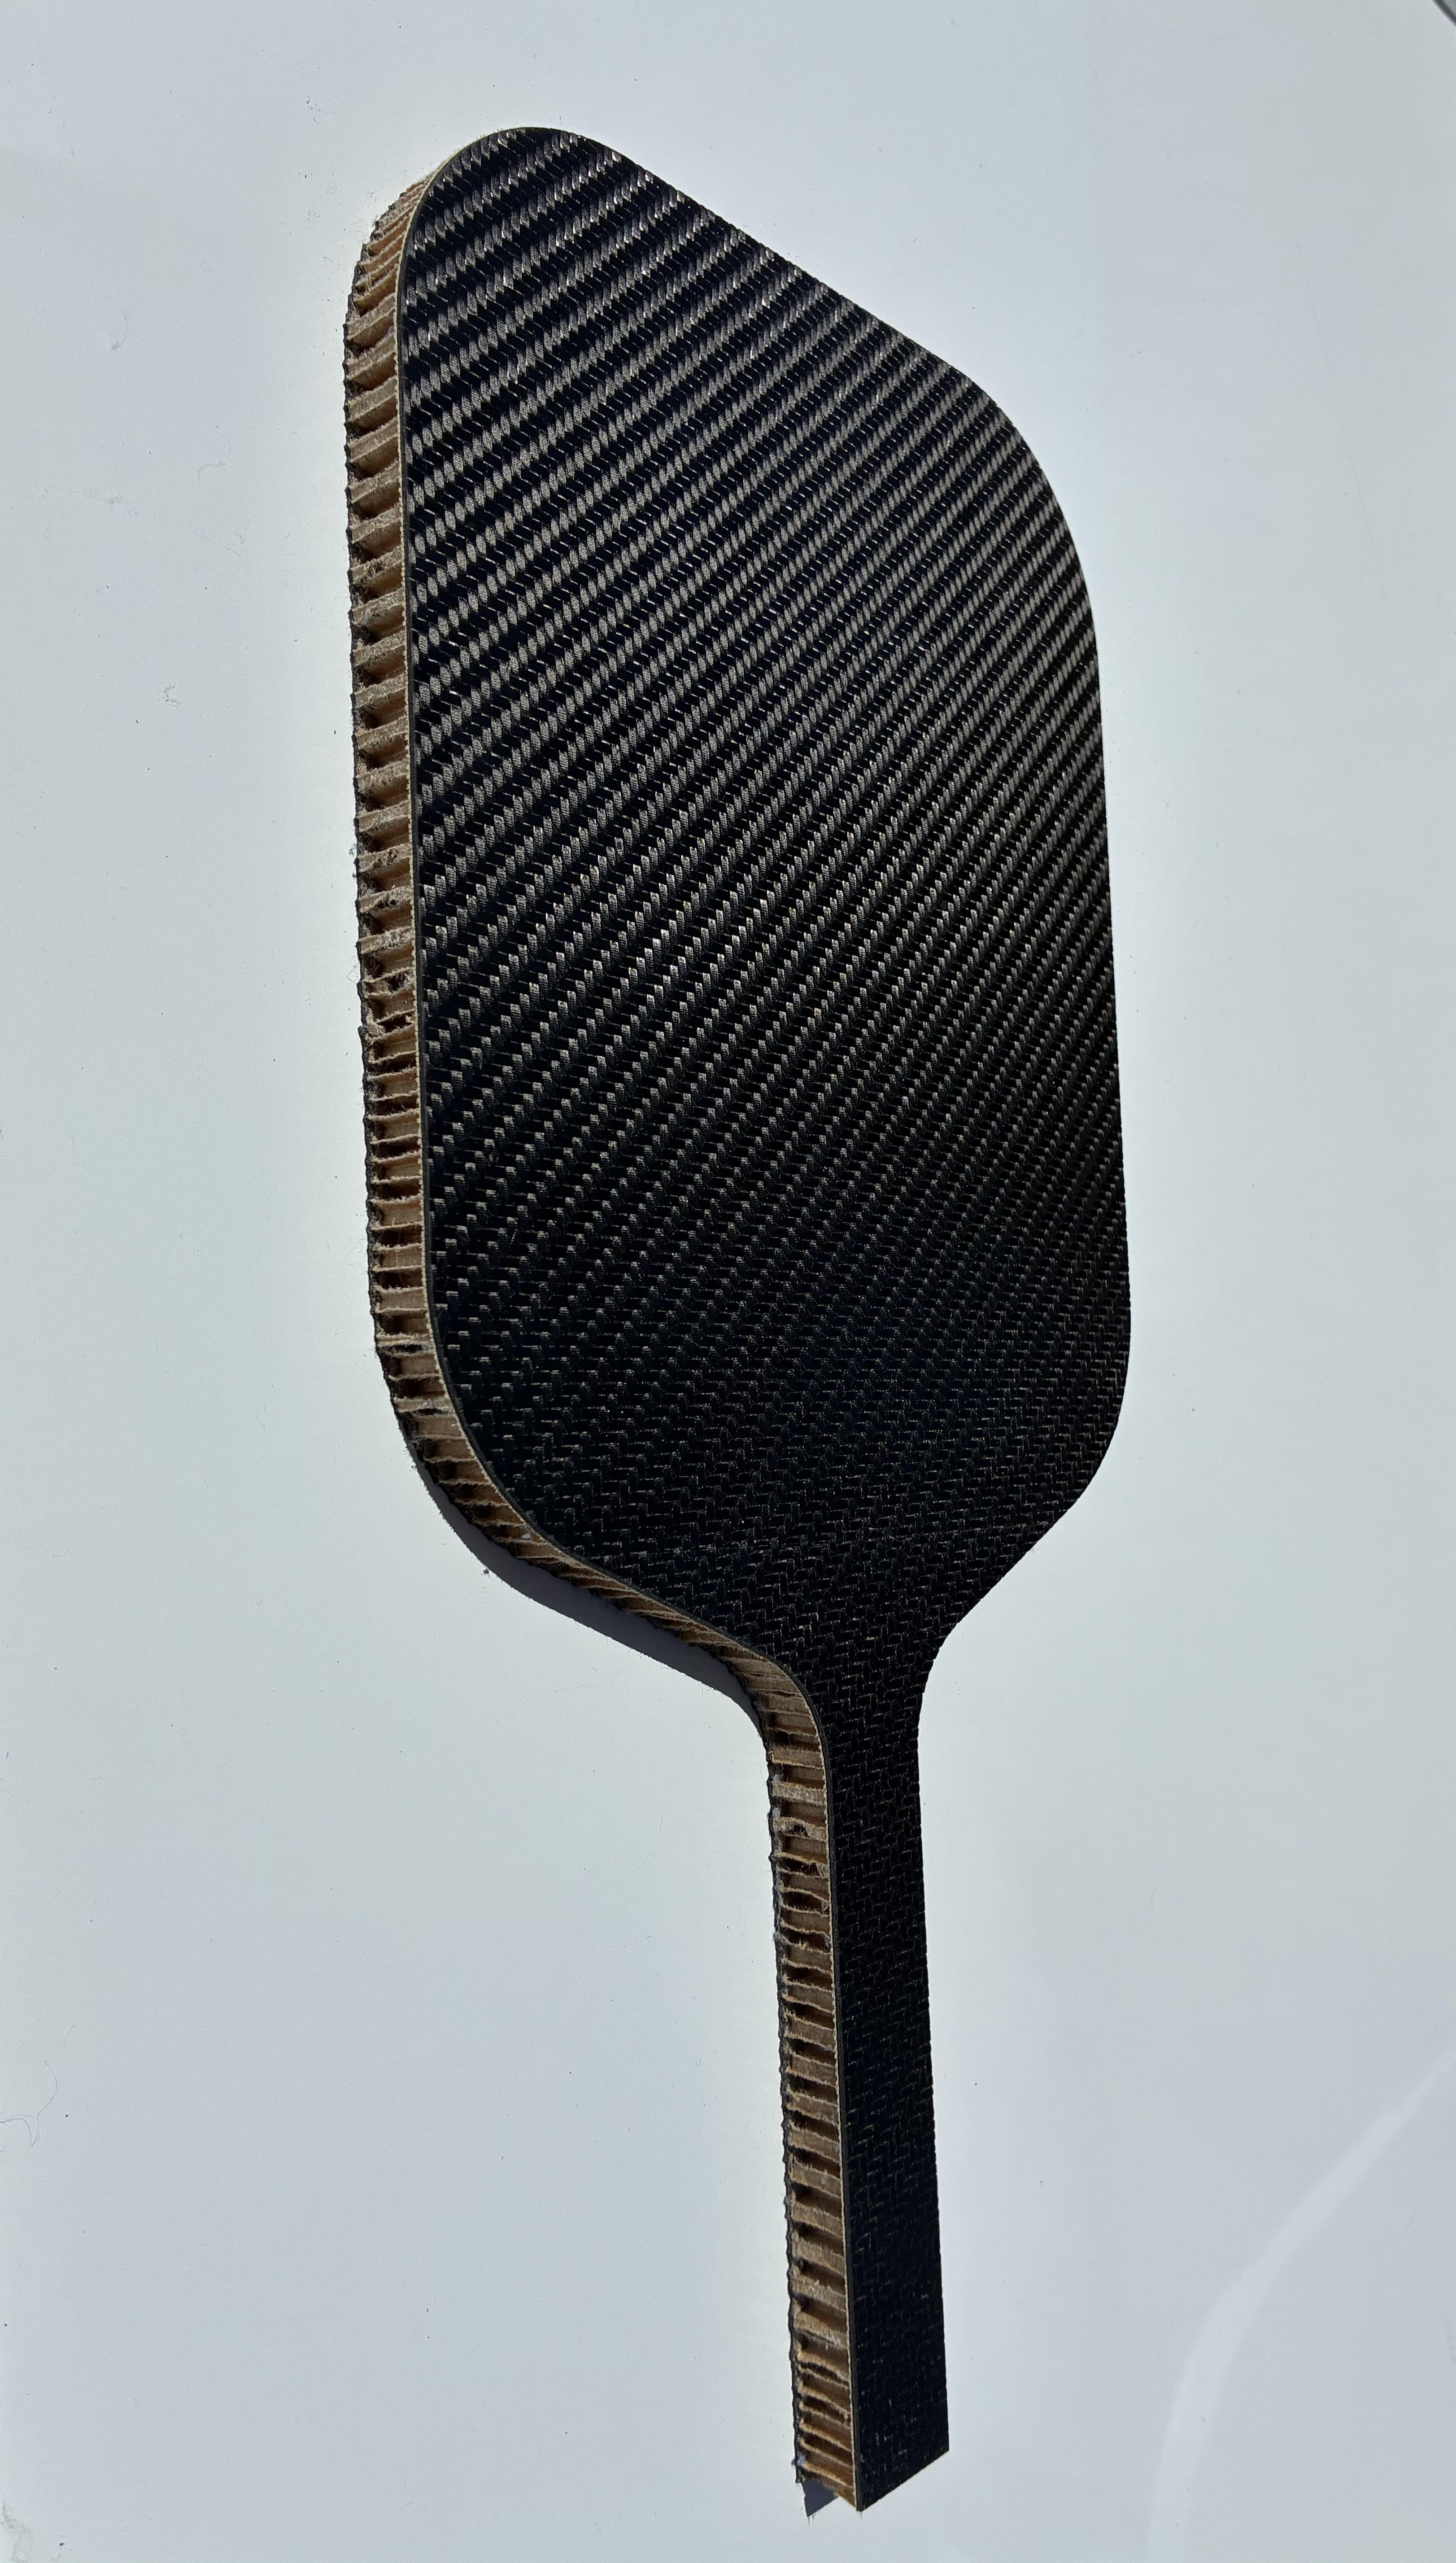
\includegraphics[
        width=1.30in,
        height=1.78in,
        keepaspectratio
    ]{side_core_view}
};

\node[
    anchor=center,
    inner sep=3pt,
    draw=RuleGray,
    line width=0.55pt,
    rounded corners=4pt
]
at ($(current page.north west)+(4.32in,-5.98in)$)
{
    \includegraphics[
        angle=-90,
        origin=c,
        width=1.30in,
        height=1.78in,
        keepaspectratio
    ]{waterjet}
};

\node[
    anchor=north,
    align=center,
    text width=1.38in,
    text=Muted,
    font=\sffamily\fontsize{6.5}{7.1}\selectfont
]
at ($(current page.north west)+(1.12in,-7.00in)$)
{Front view};

\node[
    anchor=north,
    align=center,
    text width=1.38in,
    text=Muted,
    font=\sffamily\fontsize{6.5}{7.1}\selectfont
]
at ($(current page.north west)+(2.72in,-7.00in)$)
{Core and edge profile};

\node[
    anchor=north,
    align=center,
    text width=1.38in,
    text=Muted,
    font=\sffamily\fontsize{6.5}{7.1}\selectfont
]
at ($(current page.north west)+(4.32in,-7.00in)$)
{Waterjet cutting setup};

% ============================================================
% BOTTOM RIGHT — MANUFACTURING HIGHLIGHTS
% ============================================================

\fill[SoftGreen,rounded corners=5pt]
    ($(current page.north west)+(5.18in,-5.05in)$)
    rectangle
    ($(current page.north east)+(-0.42in,-7.18in)$);

\draw[RuleGray,line width=0.55pt,rounded corners=5pt]
    ($(current page.north west)+(5.18in,-5.05in)$)
    rectangle
    ($(current page.north east)+(-0.42in,-7.18in)$);

\node[
    anchor=north west,
    text=DeepGreen,
    font=\sffamily\bfseries\fontsize{7.9}{8.6}\selectfont
]
at ($(current page.north west)+(5.44in,-5.20in)$)
{MANUFACTURING HIGHLIGHTS};

\node[
    anchor=north west,
    align=left,
    text width=5.05in,
    text=Ink,
    font=\fontsize{6.72}{7.82}\selectfont
]
at ($(current page.north west)+(5.44in,-5.49in)$)
{
\textbf{Consolidation.}
Vacuum bagging and distributed weight pressure maintained intimate contact
throughout the prepreg sandwich layup.\\[2.4pt]
\textbf{Surface quality.}
A scarce PTFE release film produced an unusually consistent matte finish
with a subtle sheen and minimal post-processing.\\[2.4pt]
\textbf{Waterjet stability.}
Perimeter weights restrained the cured stock against jet-induced lifting
and rotational moments during cutting.\\[2.4pt]
\textbf{Final assembly.}
A printed TPU edge band protected the carbon perimeter, while the PLA handle
used clearance cutouts to accommodate future stock-thickness and cutting variation.
};

% ============================================================
% RESOURCE LINK
% ============================================================

\node[
    anchor=north,
    align=center,
    text=DeepGreen,
    font=\sffamily\bfseries\fontsize{7.0}{7.6}\selectfont
]
at ($(current page.north)+(0,-7.42in)$)
{\href{\PaddleWaterjetVideo}
{\faPlayCircle\ WATERJET PICKLEBALL PADDLE DEMONSTRATION}};

% ============================================================
% FOOTER
% ============================================================

\node[
    anchor=south west,
    text=white,
    font=\sffamily\bfseries\fontsize{7.1}{7.7}\selectfont
]
at ($(current page.south west)+(0.42in,0.17in)$)
{\hyperlink{toro-results}{\faArrowLeft\ TORO COVER}};

\node[
    anchor=south,
    text=white,
    font=\sffamily\fontsize{7.0}{7.6}\selectfont
]
at ($(current page.south)+(0,0.17in)$)
{PICKLEBALL PADDLE \hspace{6pt} 1 / 1};

\node[
    anchor=south east,
    text=white,
    font=\sffamily\bfseries\fontsize{7.1}{7.7}\selectfont
]
at ($(current page.south east)+(-0.42in,0.17in)$)
{NEXT PROJECT \faArrowRight};

\end{tikzpicture}
%\input{Beam}
%\clearpage

\clearpage
.
% 2. In main.tex, place 
% ============================================================
% TORO COVER — THREE-PAGE PORTFOLIO CASE STUDY
% Pages 3–5 of the complete portfolio
%
% IMPORTANT:
% 1. This file must NOT contain \documentclass, \begin{document},
%    \end{document}, or 
% ============================================================
% TORO COVER — THREE-PAGE PORTFOLIO CASE STUDY
% Pages 3–5 of the complete portfolio
%
% IMPORTANT:
% 1. This file must NOT contain \documentclass, \begin{document},
%    \end{document}, or \input{toro}.
% 2. In main.tex, place \input{toro} before \end{document}.
% 3. Image references use the original Overleaf base filenames
%    without extensions.
% ============================================================



% ============================================================
% CLICKABLE PROJECT RESOURCES
% All links use the exact Google Drive resources supplied.
% ============================================================
\providecommand{\ToroDrawingLink}{https://drive.google.com/file/d/1A7-7wMnRNLuQDaTgxeuUCBsGNqyXzOGV/view?usp=sharing}
\providecommand{\ToroDimensionsLink}{https://drive.google.com/file/d/13sw3BNJvE8GdzlRffxoF2n5r9Gzxide7/view?usp=sharing}
\providecommand{\ToroProblemLink}{https://drive.google.com/file/d/1zHtl8zrb13F1yeN74ptawpfS5UM_xsuw/view?usp=drive_link}
\providecommand{\ToroReportLink}{https://drive.google.com/file/d/1ULZ-P46lFsC2x29ZfmRVIKgYnr9o8hMt/view?usp=drive_link}
\providecommand{\ToroPosterLink}{https://drive.google.com/file/d/1vKiKaJUcHQb_db-FkZnRF6EvtuM4hKyS/view?usp=drive_link}
\providecommand{\ToroDeploymentLink}{https://drive.google.com/file/d/1XJx34o80_mZPTl7xy93HtWAgtS3ThhvY/view?usp=drive_link}
\providecommand{\ToroRemovalLink}{https://drive.google.com/file/d/1O7xYeyB67NUwT-j1B1HeiCcHnZDYjk6_/view?usp=drive_link}

% ============================================================
% PAGE 1 — PROJECT OVERVIEW, OWNERSHIP, AND ARCHITECTURE
% ============================================================

\clearpage
\thispagestyle{empty}
\hypertarget{toro}{}
\null

\begin{tikzpicture}[remember picture,overlay]

% Background
\fill[white]
    (current page.south west)
    rectangle
    (current page.north east);

% Page bars
\fill[DeepGreen]
    (current page.north west)
    rectangle
    ($(current page.north east)+(0,-0.095in)$);

\fill[PolyGold]
    ($(current page.north west)+(0,-0.095in)$)
    rectangle
    ($(current page.north east)+(0,-0.14in)$);

\fill[DeepGreen]
    (current page.south west)
    rectangle
    ($(current page.south east)+(0,0.36in)$);

\fill[PolyGold]
    ($(current page.south west)+(0,0.36in)$)
    rectangle
    ($(current page.south east)+(0,0.405in)$);

% Header
\node[
    anchor=north west,
    text=PolyGold,
    font=\sffamily\bfseries\fontsize{8.1}{8.7}\selectfont
]
at ($(current page.north west)+(0.42in,-0.39in)$)
{01 COMPOSITES \hspace{5pt}/\hspace{5pt} PROJECT 01};

\node[
    anchor=north west,
    text=DeepGreen,
    font=\bfseries\fontsize{23.5}{24.5}\selectfont
]
at ($(current page.north west)+(0.40in,-0.67in)$)
{TORO CARBON FIBER SAFETY COVER};

\node[
    anchor=north west,
    text=Muted,
    font=\sffamily\fontsize{8.4}{9.2}\selectfont
]
at ($(current page.north west)+(0.42in,-1.12in)$)
{Cal Poly Composites Laboratory \hspace{7pt}\textbullet\hspace{7pt}
Team Project \hspace{7pt}\textbullet\hspace{7pt}
Fall--Spring 2026 \hspace{7pt}\textbullet\hspace{7pt}
San Luis Obispo, California};

\fill[PolyGold]
    ($(current page.north west)+(0.42in,-1.37in)$)
    rectangle
    ($(current page.north west)+(6.1in,-1.325in)$);

% Challenge text
\node[
    anchor=north west,
    text=DeepGreen,
    font=\sffamily\bfseries\fontsize{8.1}{8.8}\selectfont
]
at ($(current page.north west)+(0.43in,-1.61in)$)
{THE CHALLENGE};

\node[
    anchor=north west,
    align=left,
    text width=4.47in,
    text=Ink,
    font=\fontsize{8.05}{9.65}\selectfont
]
at ($(current page.north west)+(0.43in,-1.84in)$)
{
Develop a lightweight cover for a 6 ft by 6 ft in-ground spa
that could be deployed by one person, stored compactly,
provide insulation, resist a poolside environment, and maintain
a refined appearance. The sponsor supplied an ambitious but
intentionally broad project statement, requiring the team to
define the product architecture, priorities, manufacturing
strategy, and realistic path toward future commercialization.
};

% Role box
\fill[SoftGold,rounded corners=5pt]
    ($(current page.north west)+(0.42in,-2.88in)$)
    rectangle
    ($(current page.north west)+(4.98in,-4.58in)$);

\fill[PolyGold]
    ($(current page.north west)+(0.42in,-2.88in)$)
    rectangle
    ($(current page.north west)+(0.52in,-4.58in)$);

\node[
    anchor=north west,
    text=DeepGreen,
    font=\sffamily\bfseries\fontsize{8.1}{8.8}\selectfont
]
at ($(current page.north west)+(0.66in,-3.02in)$)
{MY ROLE — DESIGN \& MANUFACTURING LEAD};

\node[
    anchor=north west,
    align=left,
    text width=4.02in,
    text=Ink,
    font=\fontsize{7.05}{8.15}\selectfont
]
at ($(current page.north west)+(0.66in,-3.27in)$)
{
\textbullet\ Modeled every custom part and the complete assembly\\[1.5pt]
\textbullet\ Produced the engineering drawing package independently\\[1.5pt]
\textbullet\ Developed the composite-panel manufacturing process\\[1.5pt]
\textbullet\ Created all waterjet DXFs and manufacturing geometry\\[1.5pt]
\textbullet\ Trained teammates in wet layup and vacuum bagging\\[1.5pt]
\textbullet\ Presented feasibility, scope, and tradeoffs to the sponsor
};

% Large deployed foam-model image
\node[anchor=center,inner sep=0pt]
at ($(current page.north west)+(8.00in,-3.04in)$)
{
    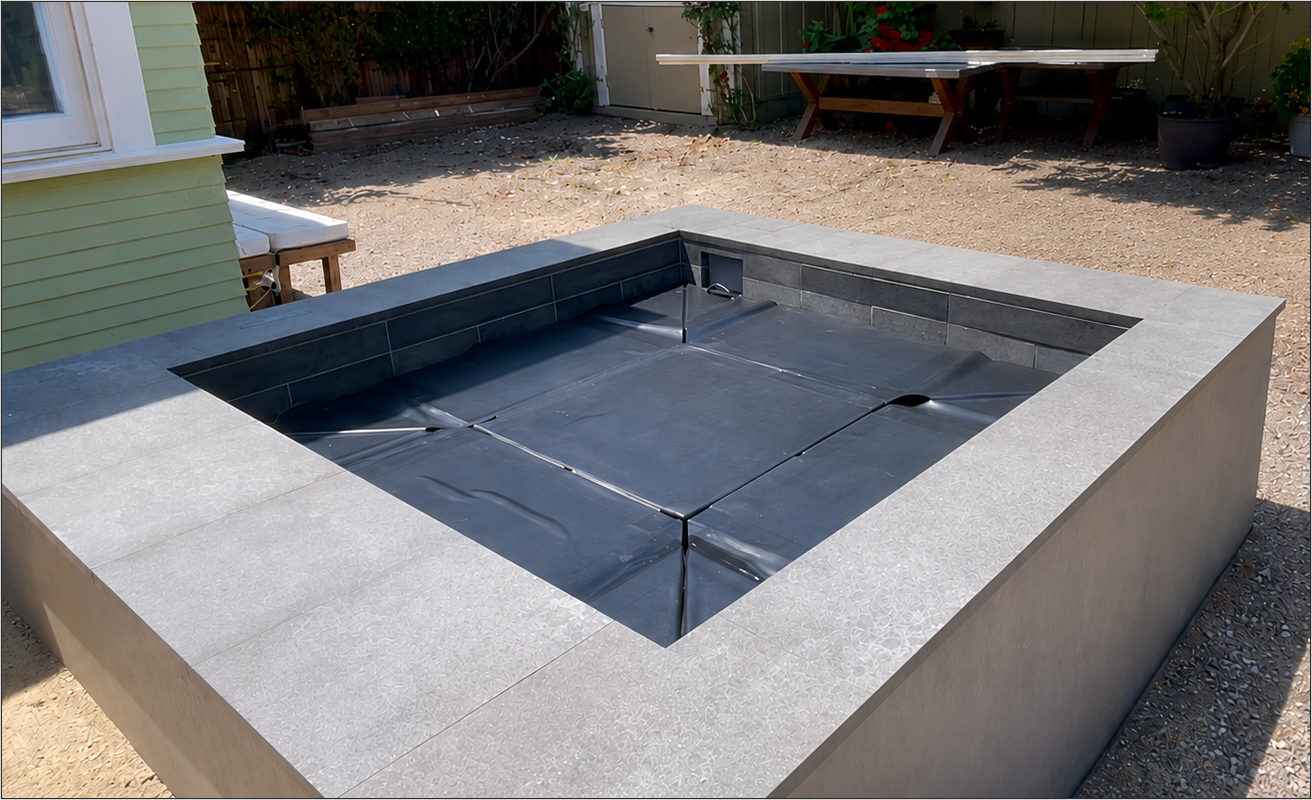
\includegraphics[
        width=5.55in,
        height=2.78in,
        keepaspectratio
    ]{deployed_functional_prototype}
};

\draw[DeepGreen,line width=0.8pt,rounded corners=7pt]
    ($(current page.north west)+(5.16in,-1.61in)$)
    rectangle
    ($(current page.north east)+(-0.42in,-4.47in)$);

\node[
    anchor=north west,
    text=Muted,
    font=\sffamily\fontsize{6.2}{6.9}\selectfont
]
at ($(current page.north west)+(5.18in,-4.54in)$)
{Functional foam model deployed over the sponsor's in-ground spa.};

% Image-strip title
\node[
    anchor=north west,
    text=DeepGreen,
    font=\sffamily\bfseries\fontsize{8.1}{8.8}\selectfont
]
at ($(current page.north west)+(0.43in,-4.78in)$)
{PRODUCT DEVELOPMENT AND FINAL ARCHITECTURE};

% Five-image development strip — CAD-first sequence
% Image 1: topside CAD
\node[anchor=center,inner sep=0pt]
at ($(current page.north west)+(1.47in,-5.73in)$)
{
    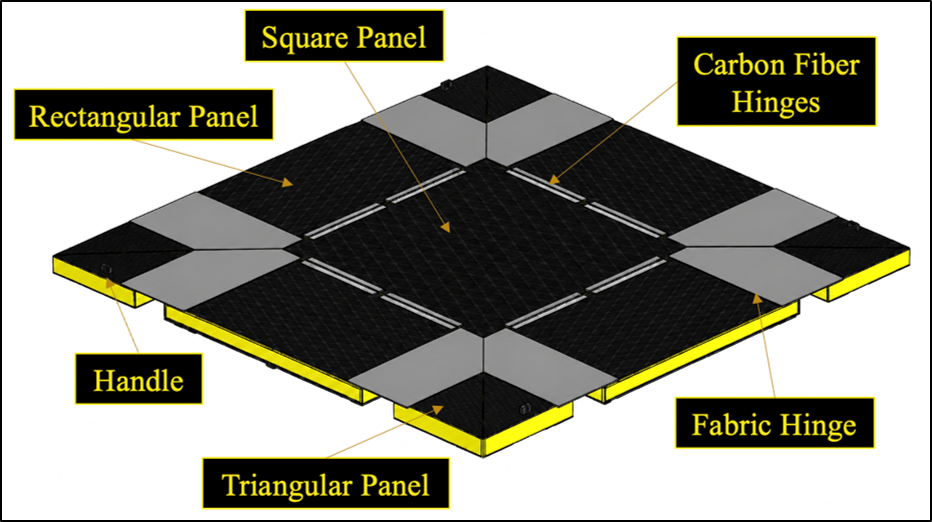
\includegraphics[
        width=1.92in,
        height=1.30in,
        keepaspectratio
    ]{Toro_Cover_topside_Cad}
};
\draw[RuleGray,line width=0.55pt,rounded corners=4pt]
    ($(current page.north west)+(0.43in,-5.04in)$)
    rectangle
    ($(current page.north west)+(2.51in,-6.43in)$);

% Image 2: underside CAD
\node[anchor=center,inner sep=0pt]
at ($(current page.north west)+(3.66in,-5.73in)$)
{
    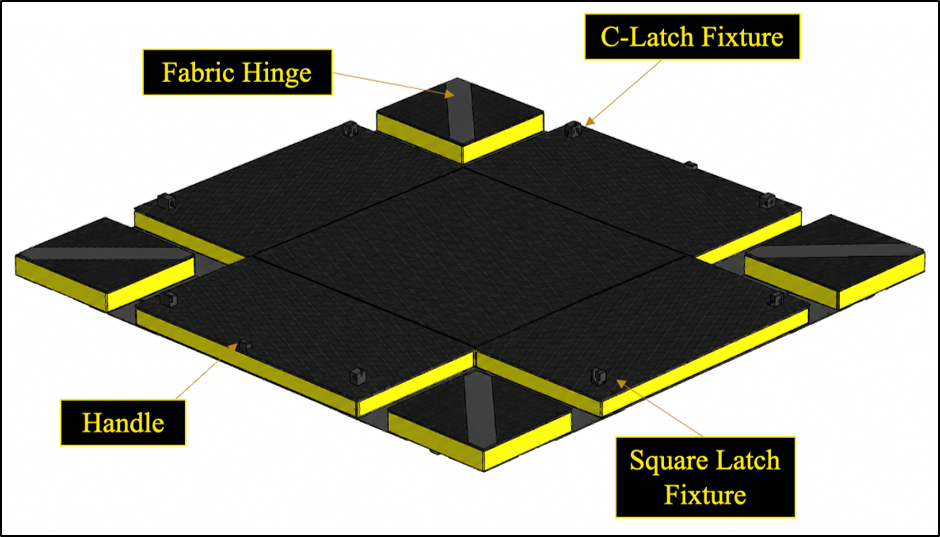
\includegraphics[
        width=1.92in,
        height=1.30in,
        keepaspectratio
    ]{toro_cover_underside_cad}
};
\draw[RuleGray,line width=0.55pt,rounded corners=4pt]
    ($(current page.north west)+(2.62in,-5.04in)$)
    rectangle
    ($(current page.north west)+(4.70in,-6.43in)$);

% Image 3: folded CAD
\node[anchor=center,inner sep=0pt]
at ($(current page.north west)+(5.85in,-5.73in)$)
{
    \includegraphics[
        width=1.92in,
        height=1.30in,
        keepaspectratio
    ]{\detokenize{Toro_Cover_folded Configuration}}
};
\draw[RuleGray,line width=0.55pt,rounded corners=4pt]
    ($(current page.north west)+(4.81in,-5.04in)$)
    rectangle
    ($(current page.north west)+(6.89in,-6.43in)$);

% Image 4: dual-use product concept
\node[anchor=center,inner sep=0pt]
at ($(current page.north west)+(8.04in,-5.73in)$)
{
    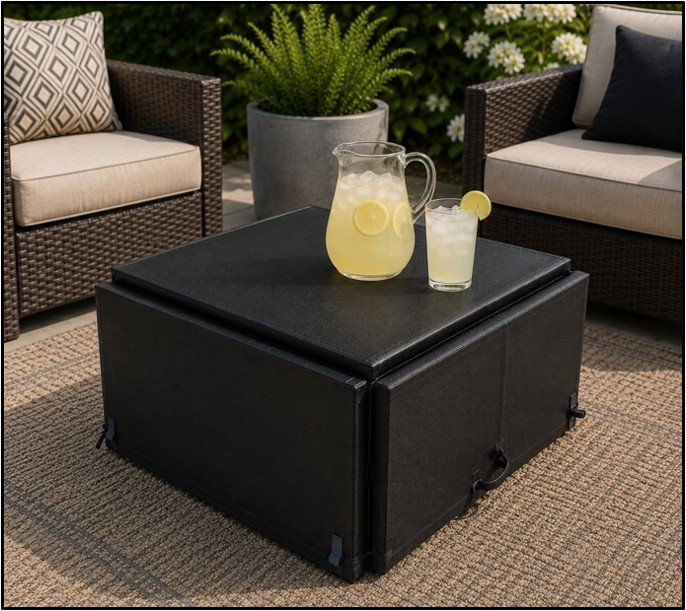
\includegraphics[
        width=1.92in,
        height=1.30in,
        keepaspectratio
    ]{generative_AI_concept_toro_cover_art}
};
\draw[RuleGray,line width=0.55pt,rounded corners=4pt]
    ($(current page.north west)+(7.00in,-5.04in)$)
    rectangle
    ($(current page.north west)+(9.08in,-6.43in)$);

% Image 5: folded foam functional prototype
% The portrait photograph is deliberately clipped to the landscape frame
% so the ottoman fills the card without extending beyond its border.
\begin{scope}
\clip[rounded corners=4pt]
    ($(current page.north west)+(9.19in,-5.04in)$)
    rectangle
    ($(current page.north east)+(-0.43in,-6.43in)$);

% Keep the original image proportions and center it within the existing card.
\node[anchor=center,inner sep=0pt]
at ($(current page.north west)+(9.88in,-5.735in)$)
{
    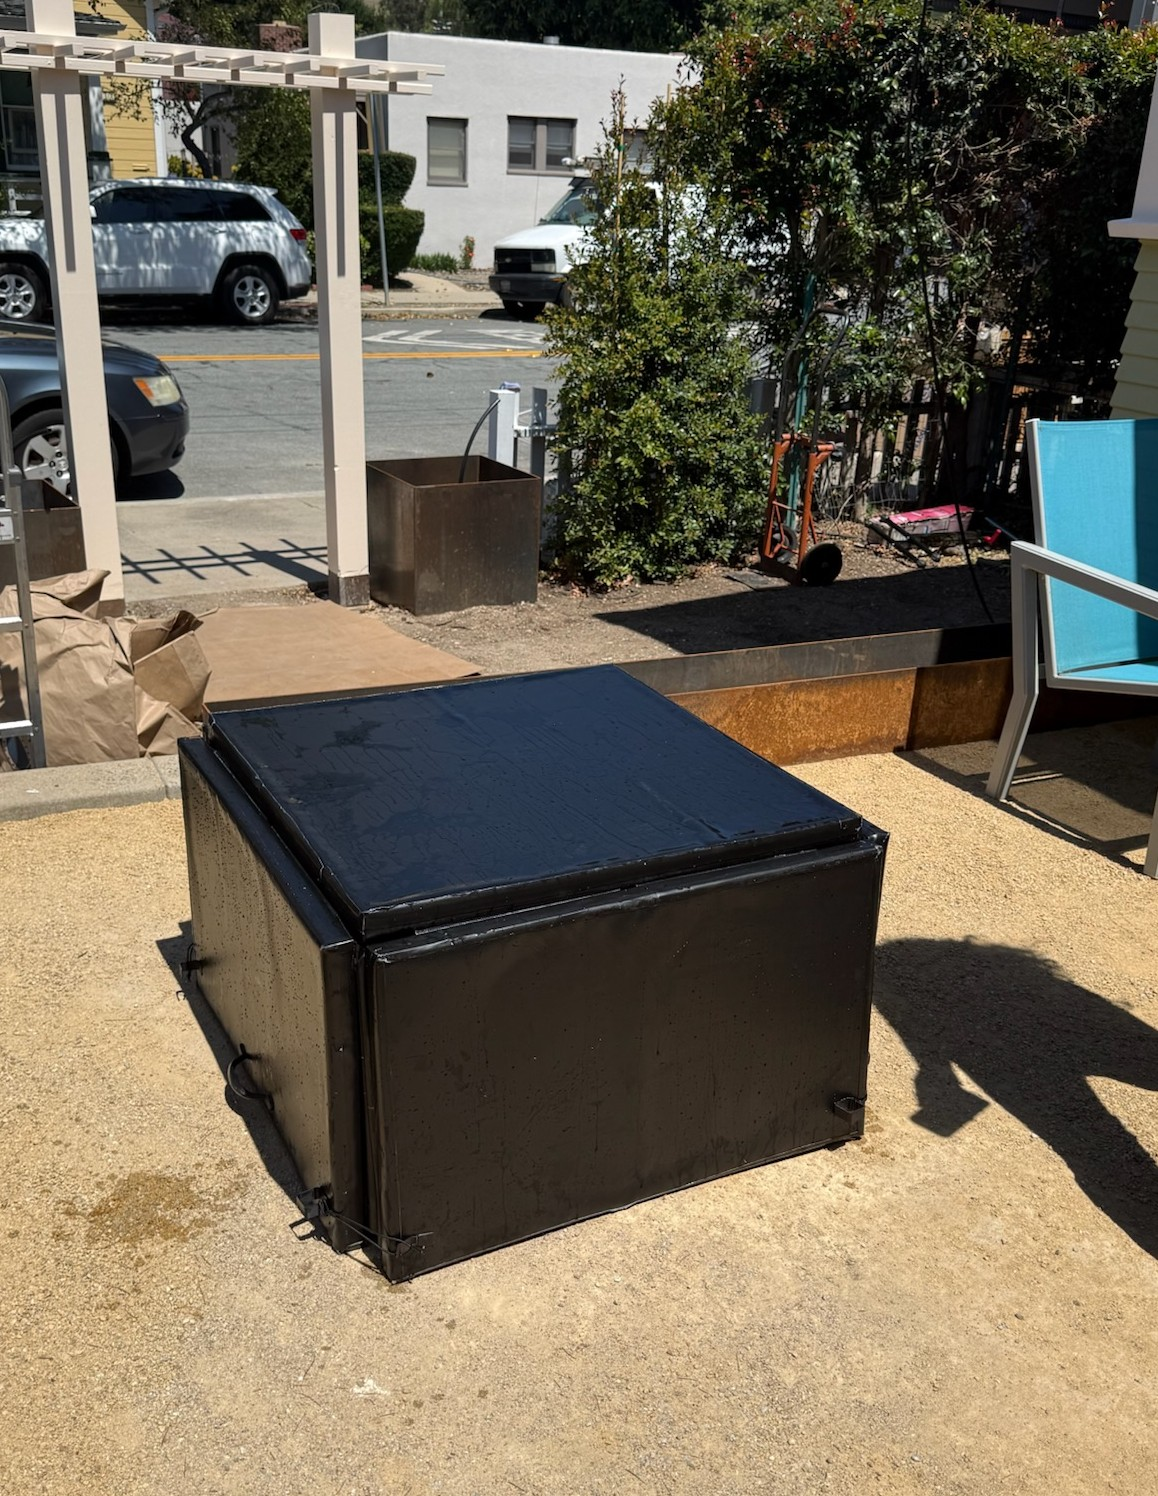
\includegraphics[
        width=1.58in,
        height=1.28in,
        keepaspectratio
    ]{foam_model_folded_backyard_image}
};
\end{scope}

\draw[RuleGray,line width=0.55pt,rounded corners=4pt]
    ($(current page.north west)+(9.19in,-5.04in)$)
    rectangle
    ($(current page.north east)+(-0.43in,-6.43in)$);

% Larger captions
\node[anchor=north,align=center,text width=1.95in,text=Muted,
      font=\sffamily\fontsize{6.8}{7.4}\selectfont]
at ($(current page.north west)+(1.47in,-6.49in)$)
{Topside panel architecture};

\node[anchor=north,align=center,text width=1.95in,text=Muted,
      font=\sffamily\fontsize{6.8}{7.4}\selectfont]
at ($(current page.north west)+(3.66in,-6.49in)$)
{Underside hinge architecture};

\node[anchor=north,align=center,text width=1.95in,text=Muted,
      font=\sffamily\fontsize{6.8}{7.4}\selectfont]
at ($(current page.north west)+(5.85in,-6.49in)$)
{Folded CAD configuration};

\node[anchor=north,align=center,text width=1.95in,text=Muted,
      font=\sffamily\fontsize{6.8}{7.4}\selectfont]
at ($(current page.north west)+(8.04in,-6.49in)$)
{Dual-use product vision};

\node[anchor=north,align=center,text width=1.95in,text=Muted,
      font=\sffamily\fontsize{6.8}{7.4}\selectfont]
at ($(current page.north west)+(9.88in,-6.49in)$)
{Folded foam prototype};

% Page 1 resource bar — centered and non-repeated resources
\fill[Panel,rounded corners=4pt]
    ($(current page.north west)+(0.43in,-7.05in)$)
    rectangle
    ($(current page.north east)+(-0.43in,-7.64in)$);
\draw[RuleGray,line width=0.5pt,rounded corners=4pt]
    ($(current page.north west)+(0.43in,-7.05in)$)
    rectangle
    ($(current page.north east)+(-0.43in,-7.64in)$);

\node[
    anchor=center,
    align=center,
    text=DeepGreen,
    font=\sffamily\bfseries\fontsize{6.9}{7.5}\selectfont
]
at ($(current page.north)+(0,-7.345in)$)
{\href{\ToroDrawingLink}{\faDraftingCompass\ DRAWING PACKAGE}
\hspace{24pt}
\href{\ToroDimensionsLink}{\faImage\ DIMENSION STUDY}
\hspace{24pt}
\href{\ToroProblemLink}{\faFileImage\ PROBLEM STATEMENT}};

% Footer
\node[
    anchor=south west,
    text=white,
    font=\sffamily\bfseries\fontsize{7.1}{7.7}\selectfont
]
at ($(current page.south west)+(0.42in,0.17in)$)
{\hyperlink{composites}{\faArrowLeft\ COMPOSITES}};

\node[
    anchor=south,
    text=white,
    font=\sffamily\fontsize{7.0}{7.6}\selectfont
]
at ($(current page.south)+(0,0.17in)$)
{TORO COVER \hspace{6pt} 1 / 3};

\node[
    anchor=south east,
    text=white,
    font=\sffamily\bfseries\fontsize{7.1}{7.7}\selectfont
]
at ($(current page.south east)+(-0.42in,0.17in)$)
{MANUFACTURING-DRIVEN DESIGN \faArrowRight};

\end{tikzpicture}


% ============================================================
% PAGE 2 — MANUFACTURING-DRIVEN DESIGN
% ============================================================

\clearpage
\thispagestyle{empty}
\hypertarget{toro-manufacturing}{}
\null

\begin{tikzpicture}[remember picture,overlay]

% Background and bars
\fill[white]
    (current page.south west)
    rectangle
    (current page.north east);

\fill[DeepGreen]
    (current page.north west)
    rectangle
    ($(current page.north east)+(0,-0.095in)$);

\fill[PolyGold]
    ($(current page.north west)+(0,-0.095in)$)
    rectangle
    ($(current page.north east)+(0,-0.14in)$);

\fill[DeepGreen]
    (current page.south west)
    rectangle
    ($(current page.south east)+(0,0.36in)$);

\fill[PolyGold]
    ($(current page.south west)+(0,0.36in)$)
    rectangle
    ($(current page.south east)+(0,0.405in)$);

% Header
\node[
    anchor=north west,
    text=PolyGold,
    font=\sffamily\bfseries\fontsize{8.1}{8.7}\selectfont
]
at ($(current page.north west)+(0.42in,-0.39in)$)
{TORO COVER \hspace{5pt}/\hspace{5pt} DESIGN FOR MANUFACTURABILITY};

\node[
    anchor=north west,
    text=DeepGreen,
    font=\bfseries\fontsize{23}{24}\selectfont
]
at ($(current page.north west)+(0.40in,-0.67in)$)
{THE ENVELOPE METHOD};

\node[
    anchor=north west,
    text=Muted,
    font=\sffamily\fontsize{8.7}{9.6}\selectfont
]
at ($(current page.north west)+(0.42in,-1.12in)$)
{A one-layup process developed for unusually thick insulated composite sandwich panels};

\fill[PolyGold]
    ($(current page.north west)+(0.42in,-1.36in)$)
    rectangle
    ($(current page.north west)+(5.30in,-1.315in)$);

% Process explanation
\fill[SoftGold,rounded corners=5pt]
    ($(current page.north west)+(0.42in,-1.61in)$)
    rectangle
    ($(current page.north east)+(-0.42in,-2.90in)$);

\fill[PolyGold]
    ($(current page.north west)+(0.42in,-1.61in)$)
    rectangle
    ($(current page.north west)+(0.52in,-2.90in)$);

\node[
    anchor=north west,
    text=DeepGreen,
    font=\sffamily\bfseries\fontsize{7.9}{8.6}\selectfont
]
at ($(current page.north west)+(0.67in,-1.76in)$)
{PROCESS INNOVATION};

\node[
    anchor=north west,
    align=left,
    text width=9.55in,
    text=Ink,
    font=\fontsize{7.35}{8.75}\selectfont
]
at ($(current page.north west)+(0.67in,-2.02in)$)
{
Weight reduction and insulation were both essential, leading to the selection of an
XPS foam core. Because XPS could not tolerate composite heat-cure temperatures, prepreg
processing was not practical and the panels had to be manufactured by wet layup with a
room-temperature cure. To simplify this process, I waterjet-cut XPS perimeter strips from
excess foam and placed them around each core inside the vacuum enclosure. Under vacuum,
the top and bottom carbon skins met along the panel sides and compressed against this
border, eliminating a separate edge-banding layup and reducing corner pleating.
};

% Workflow title
\node[
    anchor=north west,
    text=DeepGreen,
    font=\sffamily\bfseries\fontsize{8.0}{8.7}\selectfont
]
at ($(current page.north west)+(0.43in,-3.06in)$)
{MANUFACTURING WORKFLOW};

% Row 1 image 1
\node[anchor=center,inner sep=0pt]
at ($(current page.north west)+(2.07in,-4.105in)$)
{
    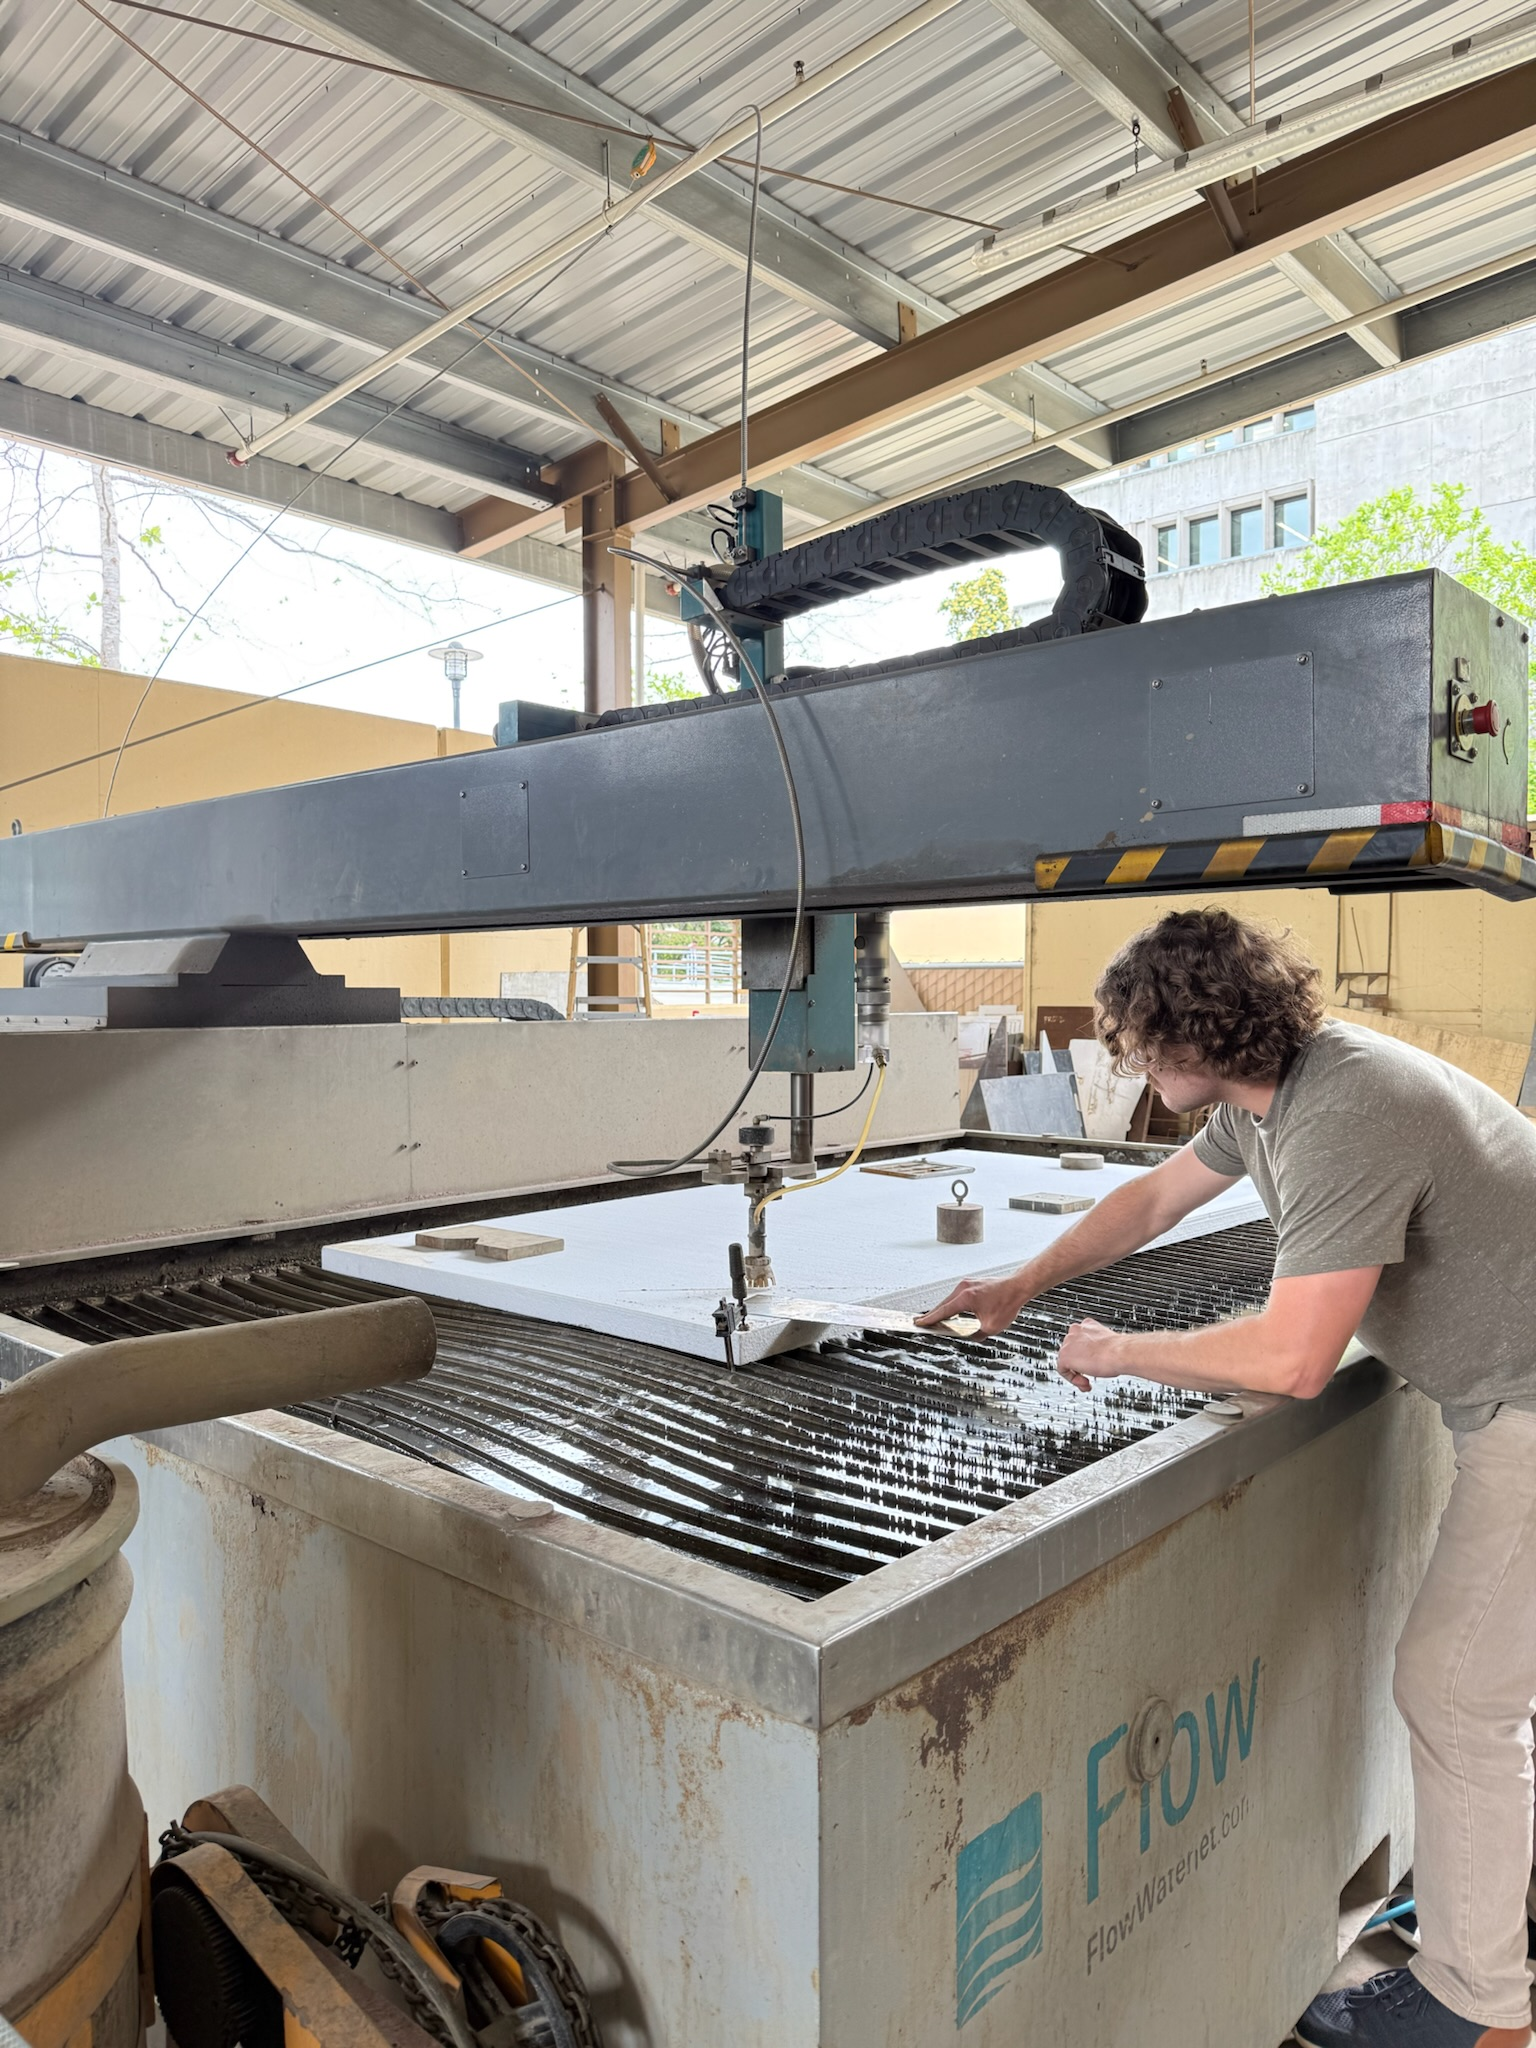
\includegraphics[
        width=3.10in,
        height=1.40in,
        keepaspectratio
    ]{waterjet_foam}
};
\draw[RuleGray,line width=0.55pt,rounded corners=4pt]
    ($(current page.north west)+(0.43in,-3.36in)$)
    rectangle
    ($(current page.north west)+(3.71in,-4.85in)$);

% Row 1 image 2
\node[anchor=center,inner sep=0pt]
at ($(current page.north west)+(5.50in,-4.105in)$)
{
    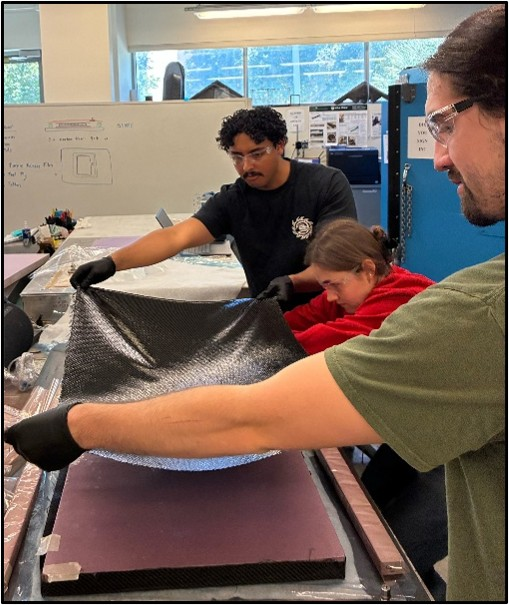
\includegraphics[
        width=3.10in,
        height=1.40in,
        keepaspectratio
    ]{group_layup}
};
\draw[RuleGray,line width=0.55pt,rounded corners=4pt]
    ($(current page.north west)+(3.86in,-3.36in)$)
    rectangle
    ($(current page.north west)+(7.14in,-4.85in)$);

% Row 1 image 3
\node[anchor=center,inner sep=0pt]
at ($(current page.north west)+(8.935in,-4.105in)$)
{
    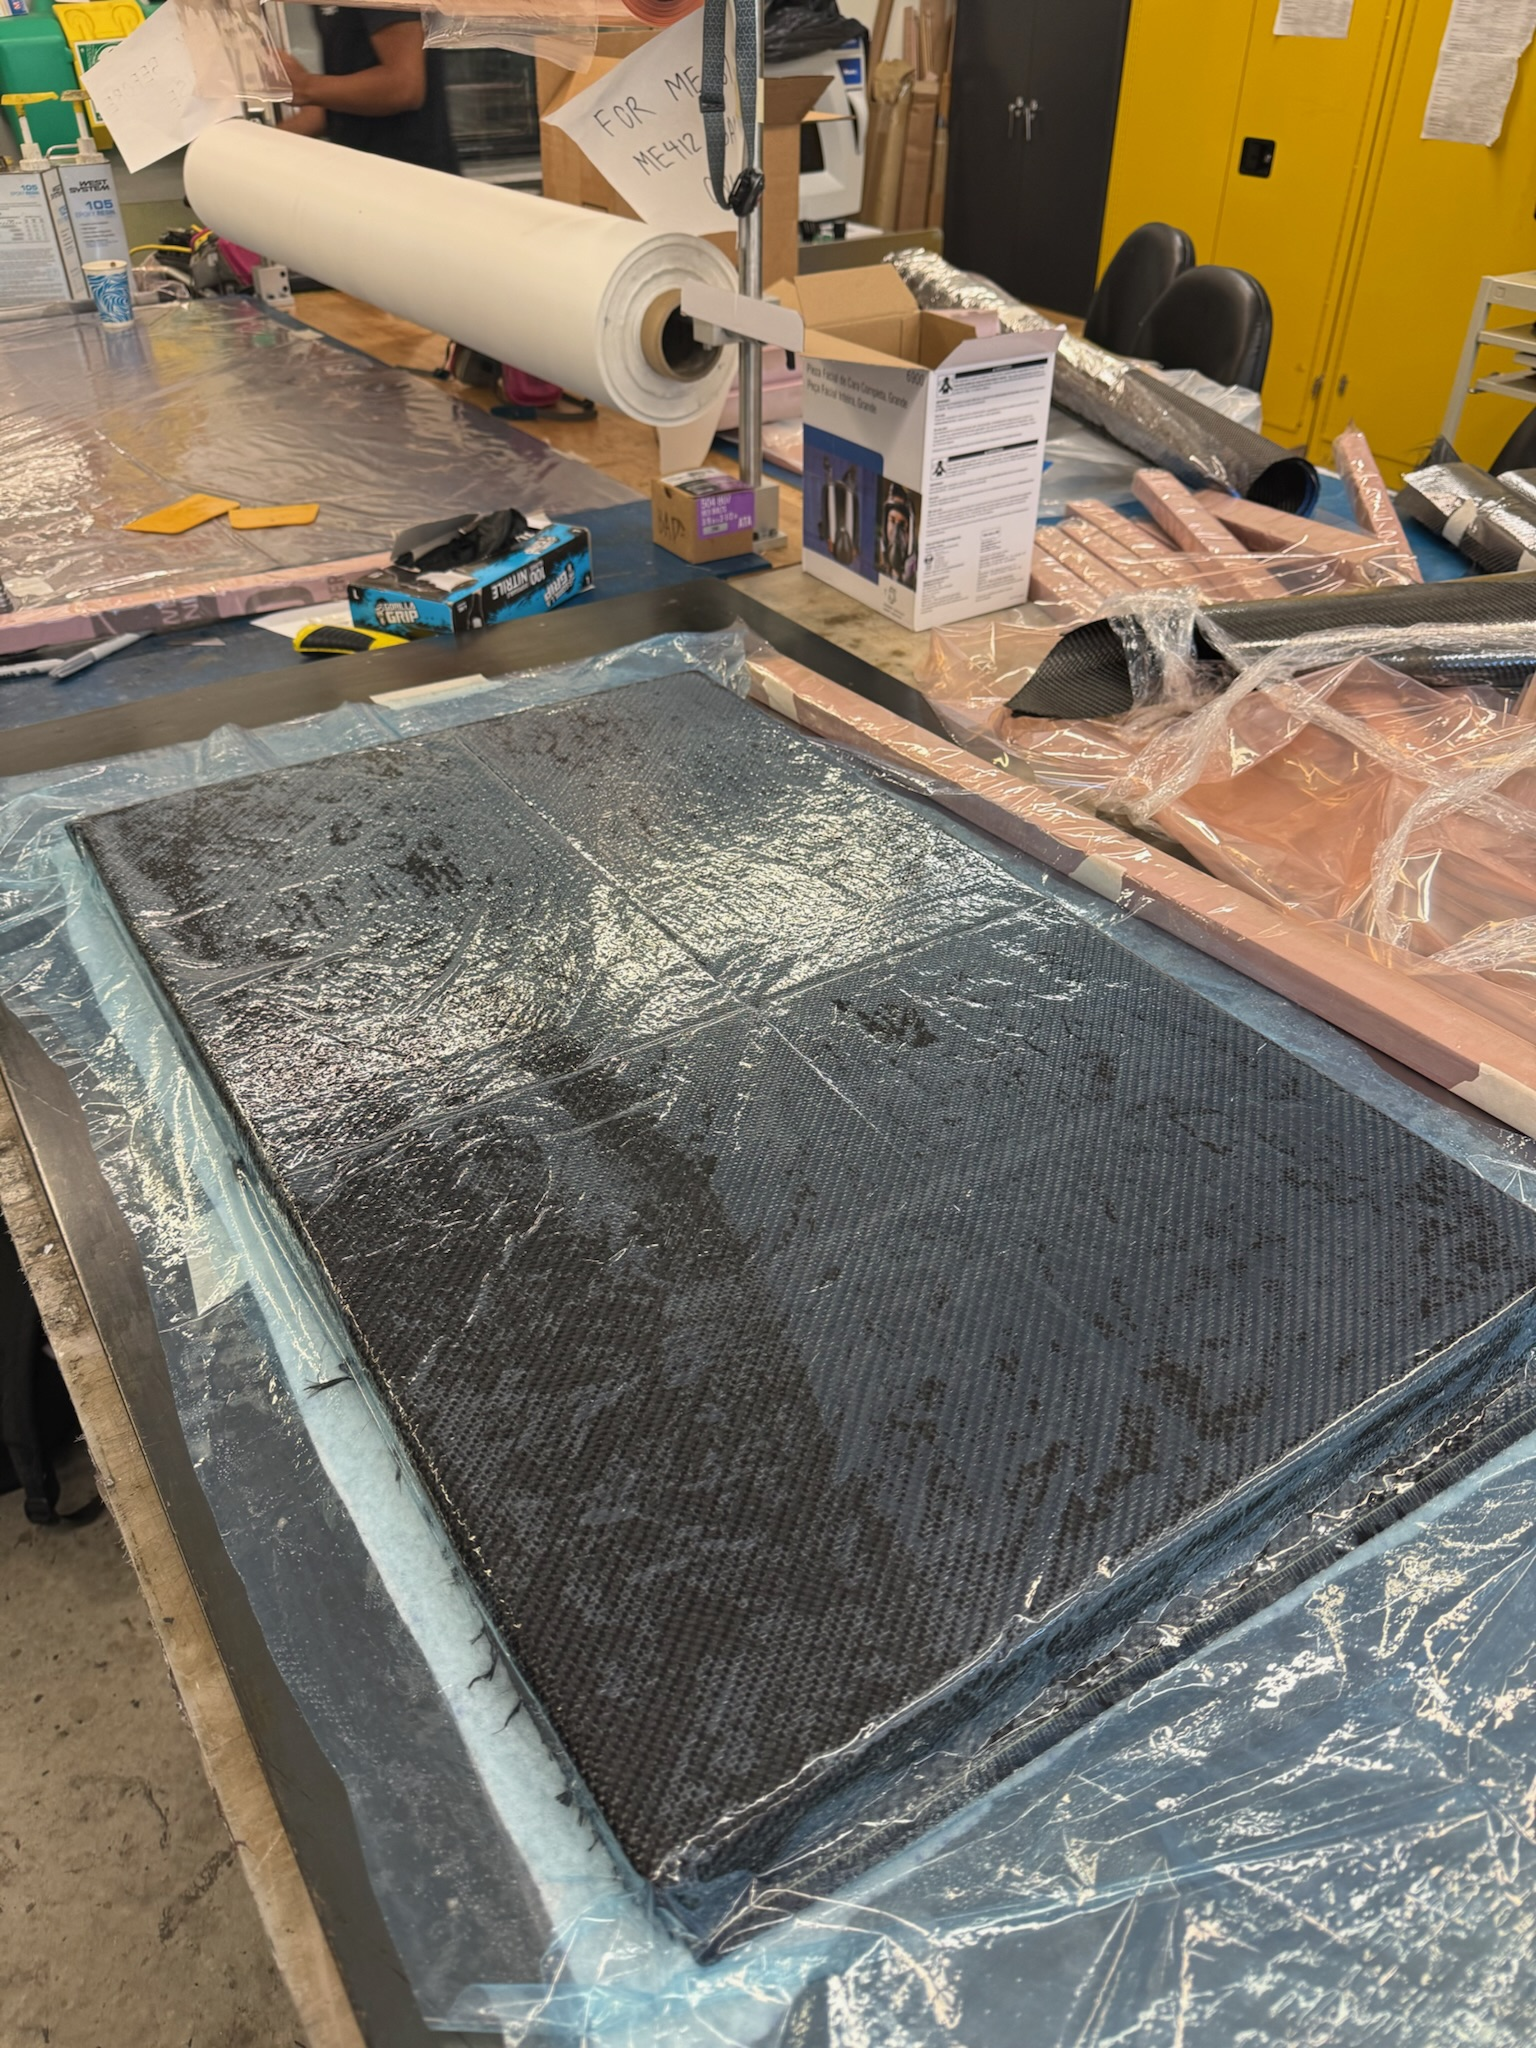
\includegraphics[
        width=3.10in,
        height=1.40in,
        keepaspectratio
    ]{blue_perforrated_film_layup}
};
\draw[RuleGray,line width=0.55pt,rounded corners=4pt]
    ($(current page.north west)+(7.29in,-3.36in)$)
    rectangle
    ($(current page.north east)+(-0.42in,-4.85in)$);

% Row 1 captions
\node[anchor=north,text=Muted,font=\sffamily\fontsize{6.7}{7.3}\selectfont]
at ($(current page.north west)+(2.07in,-4.90in)$)
{1. Waterjet-cut core and perimeter geometry};

\node[anchor=north,text=Muted,font=\sffamily\fontsize{6.7}{7.3}\selectfont]
at ($(current page.north west)+(5.50in,-4.90in)$)
{2. Team wet layup under my process guidance};

\node[anchor=north,text=Muted,font=\sffamily\fontsize{6.7}{7.3}\selectfont]
at ($(current page.north west)+(8.935in,-4.90in)$)
{3. Perforated film, breather, and vacuum enclosure};

% Row 2 image 1
\node[anchor=center,inner sep=0pt]
at ($(current page.north west)+(2.07in,-5.875in)$)
{
    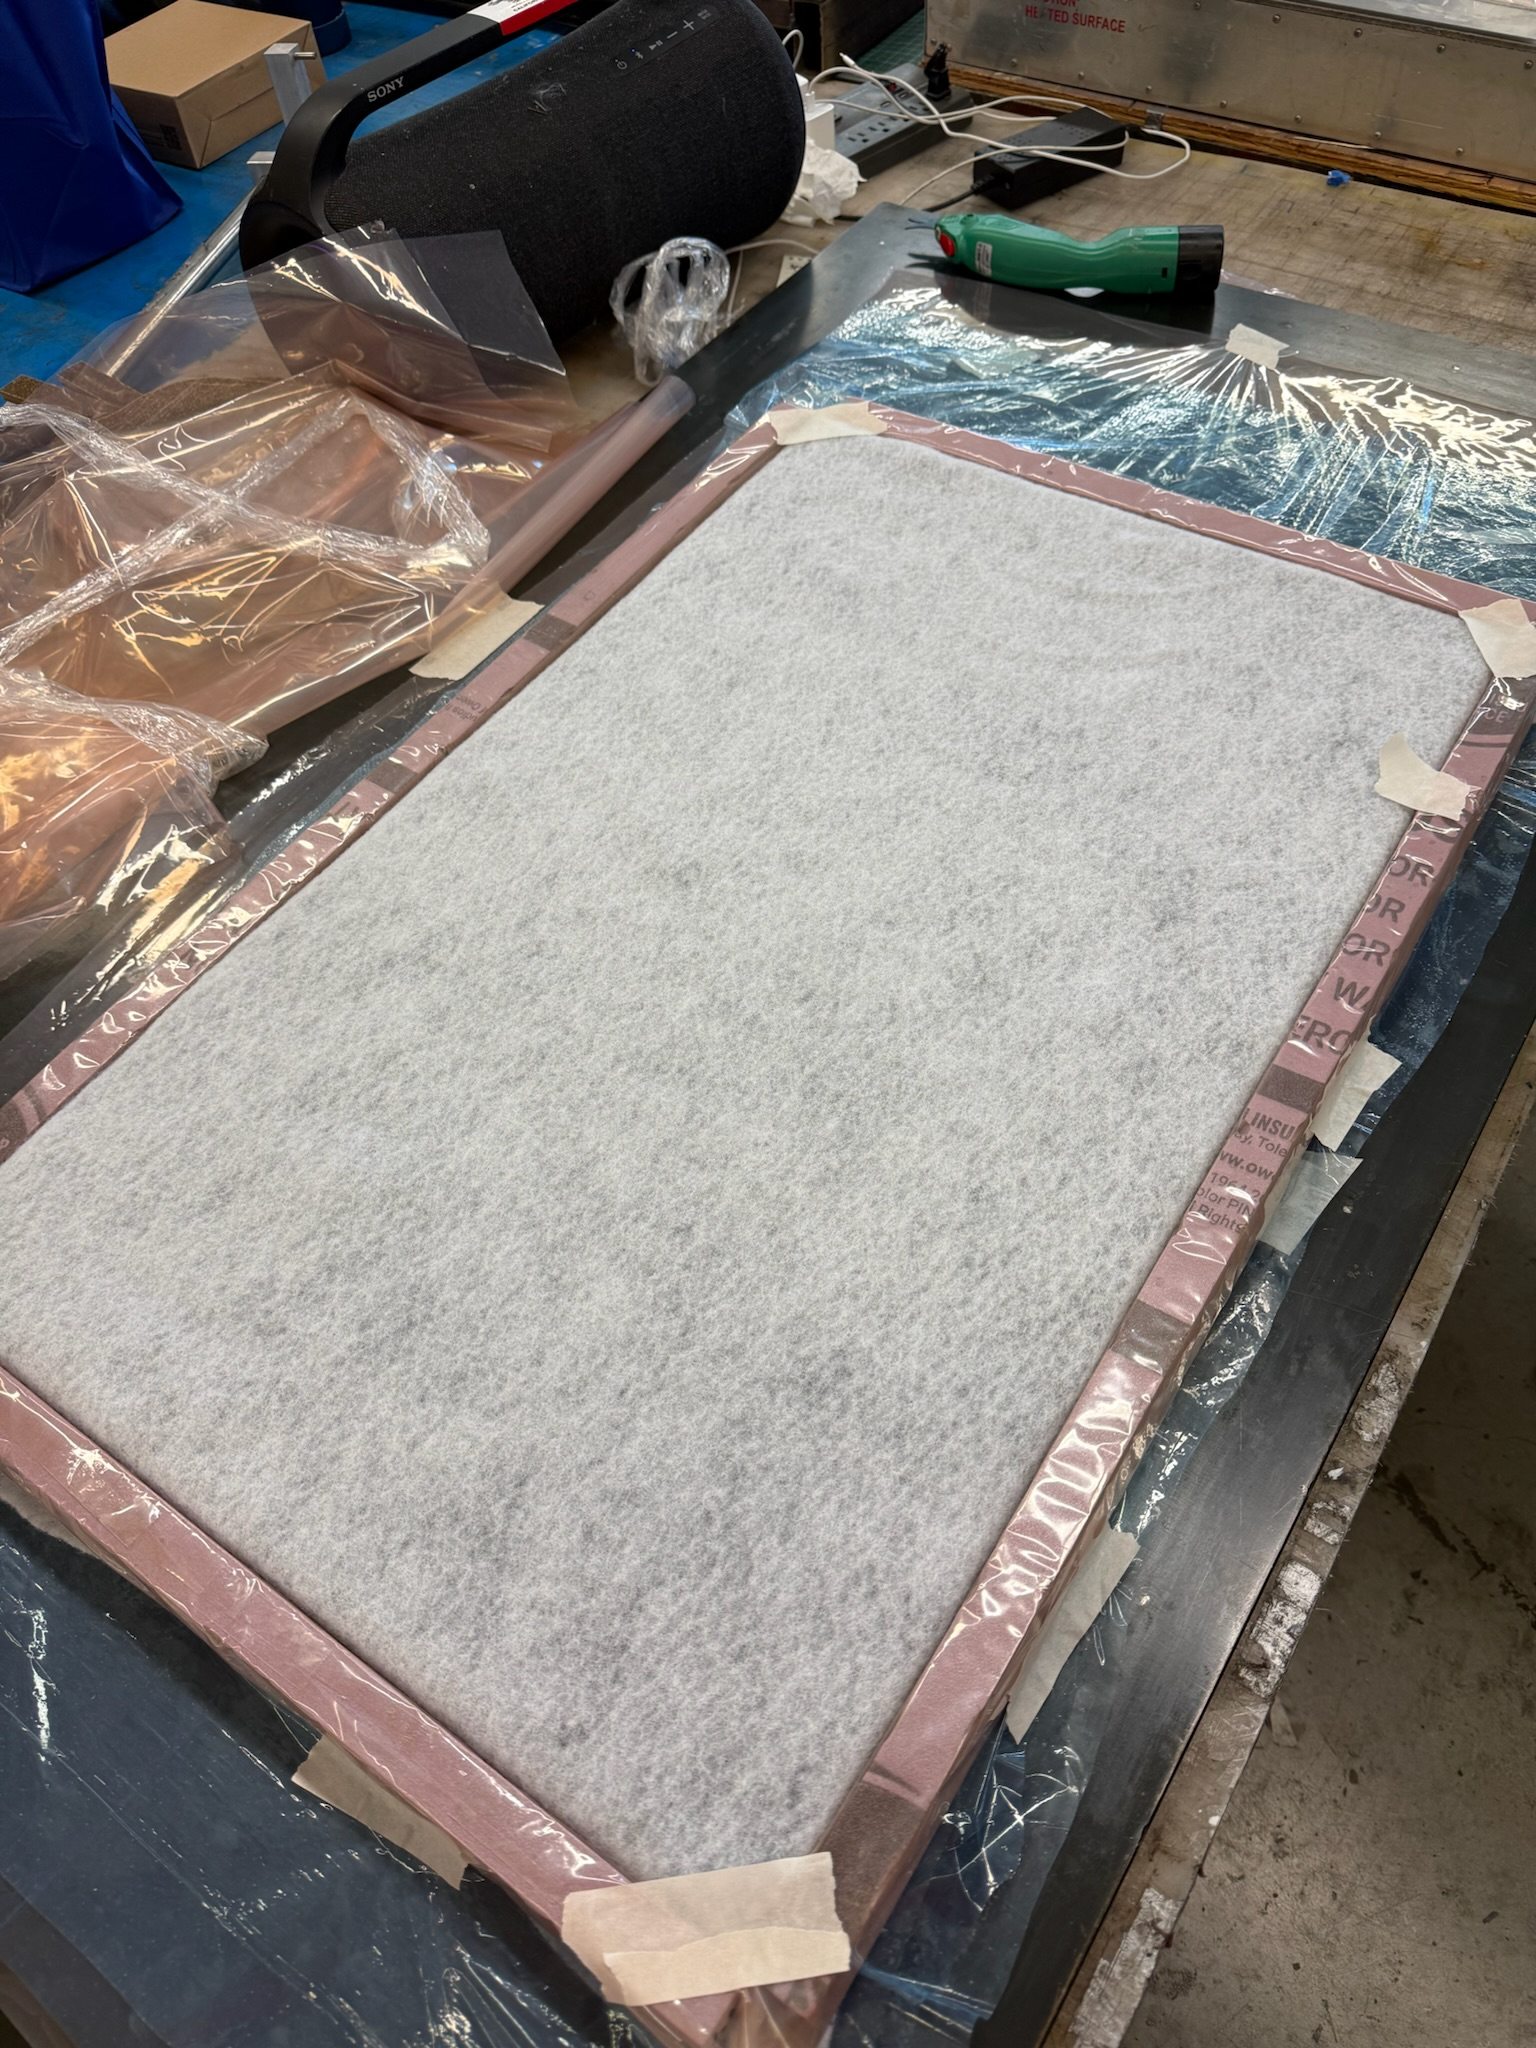
\includegraphics[
        width=3.10in,
        height=1.40in,
        keepaspectratio
    ]{completed_layup}
};
\draw[RuleGray,line width=0.55pt,rounded corners=4pt]
    ($(current page.north west)+(0.43in,-5.13in)$)
    rectangle
    ($(current page.north west)+(3.71in,-6.62in)$);

% Row 2 image 2 — oven chamber used only as a reliable vacuum enclosure; no heat applied
\node[anchor=center,inner sep=0pt]
at ($(current page.north west)+(5.50in,-5.875in)$)
{
    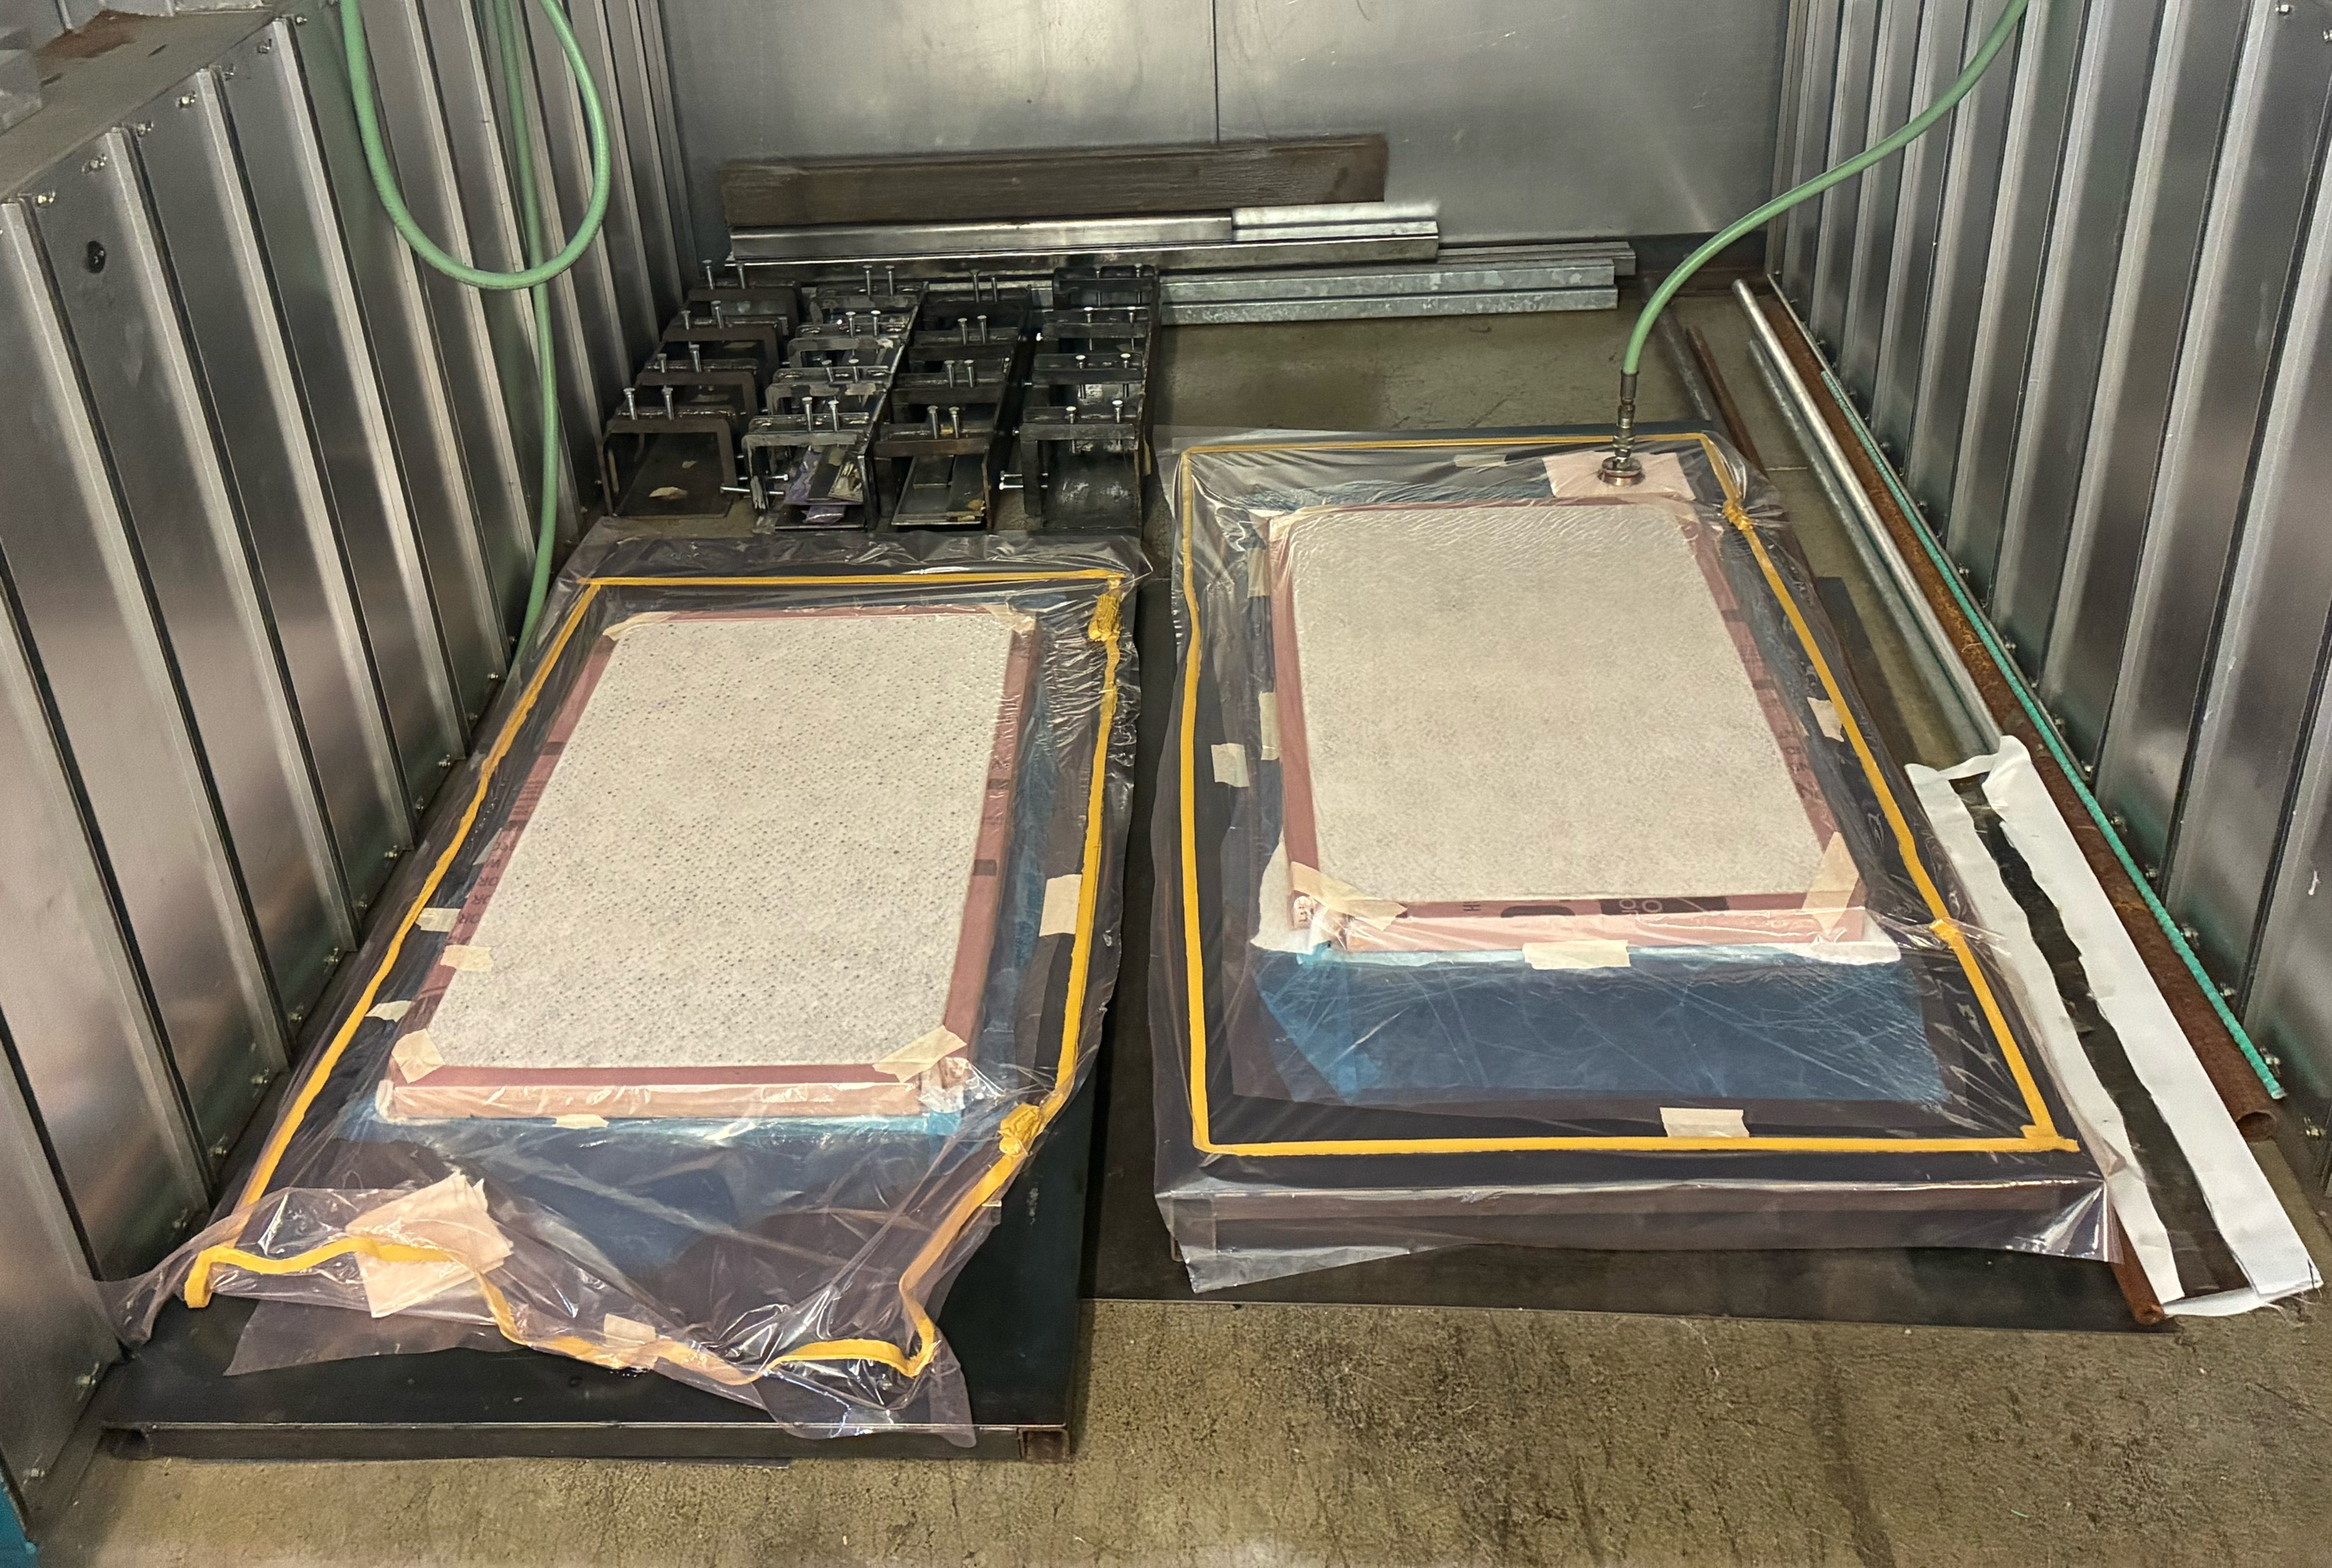
\includegraphics[
        width=3.10in,
        height=1.40in,
        keepaspectratio
    ]{layups_in_composite_oven_under_vacuumPressure}
};
\draw[RuleGray,line width=0.55pt,rounded corners=4pt]
    ($(current page.north west)+(3.86in,-5.13in)$)
    rectangle
    ($(current page.north west)+(7.14in,-6.62in)$);

% Row 2 image 3
\node[anchor=center,inner sep=0pt]
at ($(current page.north west)+(8.935in,-5.875in)$)
{
    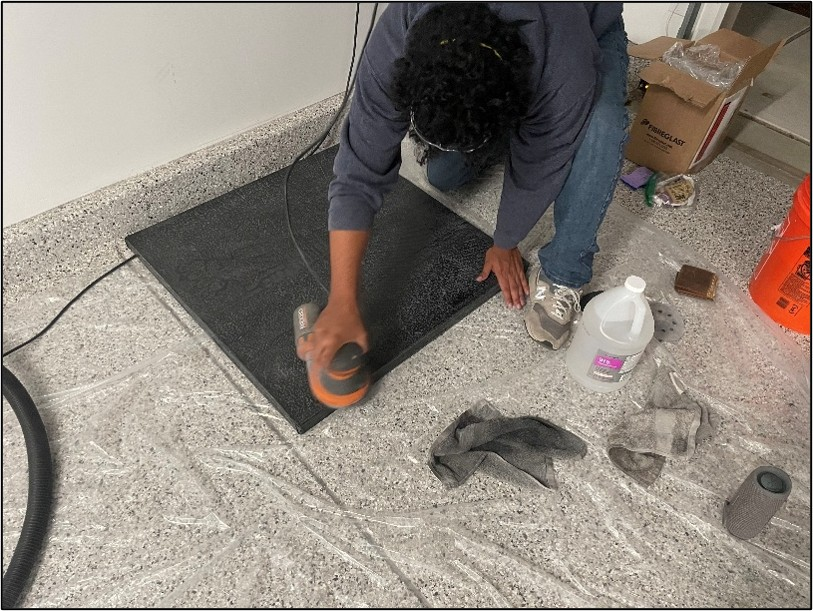
\includegraphics[
        width=3.10in,
        height=1.40in,
        keepaspectratio
    ]{garage_sanding}
};
\draw[RuleGray,line width=0.55pt,rounded corners=4pt]
    ($(current page.north west)+(7.29in,-5.13in)$)
    rectangle
    ($(current page.north east)+(-0.42in,-6.62in)$);

% Row 2 captions
\node[anchor=north,text=Muted,font=\sffamily\fontsize{6.7}{7.3}\selectfont]
at ($(current page.north west)+(2.07in,-6.67in)$)
{4. Fully saturated carbon skin and foam sandwich};

\node[anchor=north,text=Muted,font=\sffamily\fontsize{6.7}{7.3}\selectfont]
at ($(current page.north west)+(5.50in,-6.67in)$)
{5. Room-temperature cure under continuous vacuum};

\node[anchor=north,text=Muted,font=\sffamily\fontsize{6.7}{7.3}\selectfont]
at ($(current page.north west)+(8.935in,-6.67in)$)
{6. Post-processing and surface preparation};

% Bottom callouts
\fill[Panel,rounded corners=4pt]
    ($(current page.north west)+(0.43in,-6.95in)$)
    rectangle
    ($(current page.north west)+(5.48in,-7.60in)$);

\draw[RuleGray,line width=0.55pt,rounded corners=4pt]
    ($(current page.north west)+(0.43in,-6.95in)$)
    rectangle
    ($(current page.north west)+(5.48in,-7.60in)$);

\node[
    anchor=north west,
    text=DeepGreen,
    font=\sffamily\bfseries\fontsize{7.0}{7.6}\selectfont
]
at ($(current page.north west)+(0.63in,-7.08in)$)
{FROM THREE LAYUPS TO ONE};

\node[
    anchor=north west,
    align=left,
    text width=4.56in,
    text=Ink,
    font=\fontsize{6.45}{7.45}\selectfont
]
at ($(current page.north west)+(0.63in,-7.29in)$)
{
The Envelope Method reduced labor, cure cycles, handling,
alignment risk, and time spent forming numerous vacuum-bag
pleats around the 1.5-inch-thick XPS panels.
};

\fill[Panel,rounded corners=4pt]
    ($(current page.north west)+(5.68in,-6.95in)$)
    rectangle
    ($(current page.north east)+(-0.42in,-7.60in)$);

\draw[RuleGray,line width=0.55pt,rounded corners=4pt]
    ($(current page.north west)+(5.68in,-6.95in)$)
    rectangle
    ($(current page.north east)+(-0.42in,-7.60in)$);

\node[
    anchor=north west,
    text=DeepGreen,
    font=\sffamily\bfseries\fontsize{7.0}{7.6}\selectfont
]
at ($(current page.north west)+(5.88in,-7.08in)$)
{WHY SURFACE-BONDED HARDWARE};

\node[
    anchor=north west,
    align=left,
    text width=4.55in,
    text=Ink,
    font=\fontsize{6.45}{7.45}\selectfont
]
at ($(current page.north west)+(5.88in,-7.29in)$)
{
Adhesively bonded hinges and fixtures preserved the clean
composite exterior and avoided drilled inserts, foam-core
crushing, added stress concentrations, and new leak paths.
};


% Footer
\node[
    anchor=south west,
    text=white,
    font=\sffamily\bfseries\fontsize{7.1}{7.7}\selectfont
]
at ($(current page.south west)+(0.42in,0.17in)$)
{\faArrowLeft\ PRODUCT ARCHITECTURE};

\node[
    anchor=south,
    text=white,
    font=\sffamily\fontsize{7.0}{7.6}\selectfont
]
at ($(current page.south)+(0,0.17in)$)
{TORO COVER \hspace{6pt} 2 / 3};

\node[
    anchor=south east,
    text=white,
    font=\sffamily\bfseries\fontsize{7.1}{7.7}\selectfont
]
at ($(current page.south east)+(-0.42in,0.17in)$)
{VALIDATION \& TAKEAWAYS \faArrowRight};

\end{tikzpicture}


% ============================================================
% PAGE 3 — FINISHING, VALIDATION, AND TAKEAWAYS
% ============================================================

\clearpage
\thispagestyle{empty}
\hypertarget{toro-results}{}
\null

\begin{tikzpicture}[remember picture,overlay]

% Background and bars
\fill[white]
    (current page.south west)
    rectangle
    (current page.north east);

\fill[DeepGreen]
    (current page.north west)
    rectangle
    ($(current page.north east)+(0,-0.095in)$);

\fill[PolyGold]
    ($(current page.north west)+(0,-0.095in)$)
    rectangle
    ($(current page.north east)+(0,-0.14in)$);

\fill[DeepGreen]
    (current page.south west)
    rectangle
    ($(current page.south east)+(0,0.36in)$);

\fill[PolyGold]
    ($(current page.south west)+(0,0.36in)$)
    rectangle
    ($(current page.south east)+(0,0.405in)$);

% Header
\node[
    anchor=north west,
    text=PolyGold,
    font=\sffamily\bfseries\fontsize{8.1}{8.7}\selectfont
]
at ($(current page.north west)+(0.42in,-0.39in)$)
{TORO COVER \hspace{5pt}/\hspace{5pt} VALIDATION AND ENGINEERING TAKEAWAYS};

\node[
    anchor=north west,
    text=DeepGreen,
    font=\bfseries\fontsize{22.5}{23.5}\selectfont
]
at ($(current page.north west)+(0.40in,-0.67in)$)
{FROM PROTOTYPE TO PRODUCT PATHWAY};

\node[
    anchor=north west,
    text=Muted,
    font=\sffamily\fontsize{8.7}{9.6}\selectfont
]
at ($(current page.north west)+(0.42in,-1.12in)$)
{Environmental protection, usability testing, scope decisions, and lessons from technical leadership};

\fill[PolyGold]
    ($(current page.north west)+(0.42in,-1.36in)$)
    rectangle
    ($(current page.north west)+(5.8in,-1.315in)$);

% Finishing title
\node[
    anchor=north west,
    text=DeepGreen,
    font=\sffamily\bfseries\fontsize{8.0}{8.7}\selectfont
]
at ($(current page.north west)+(0.43in,-1.62in)$)
{OUTDOOR FINISHING AND ENVIRONMENTAL PROTECTION};

% Image 1
\node[anchor=center,inner sep=0pt]
at ($(current page.north west)+(1.705in,-2.655in)$)
{
    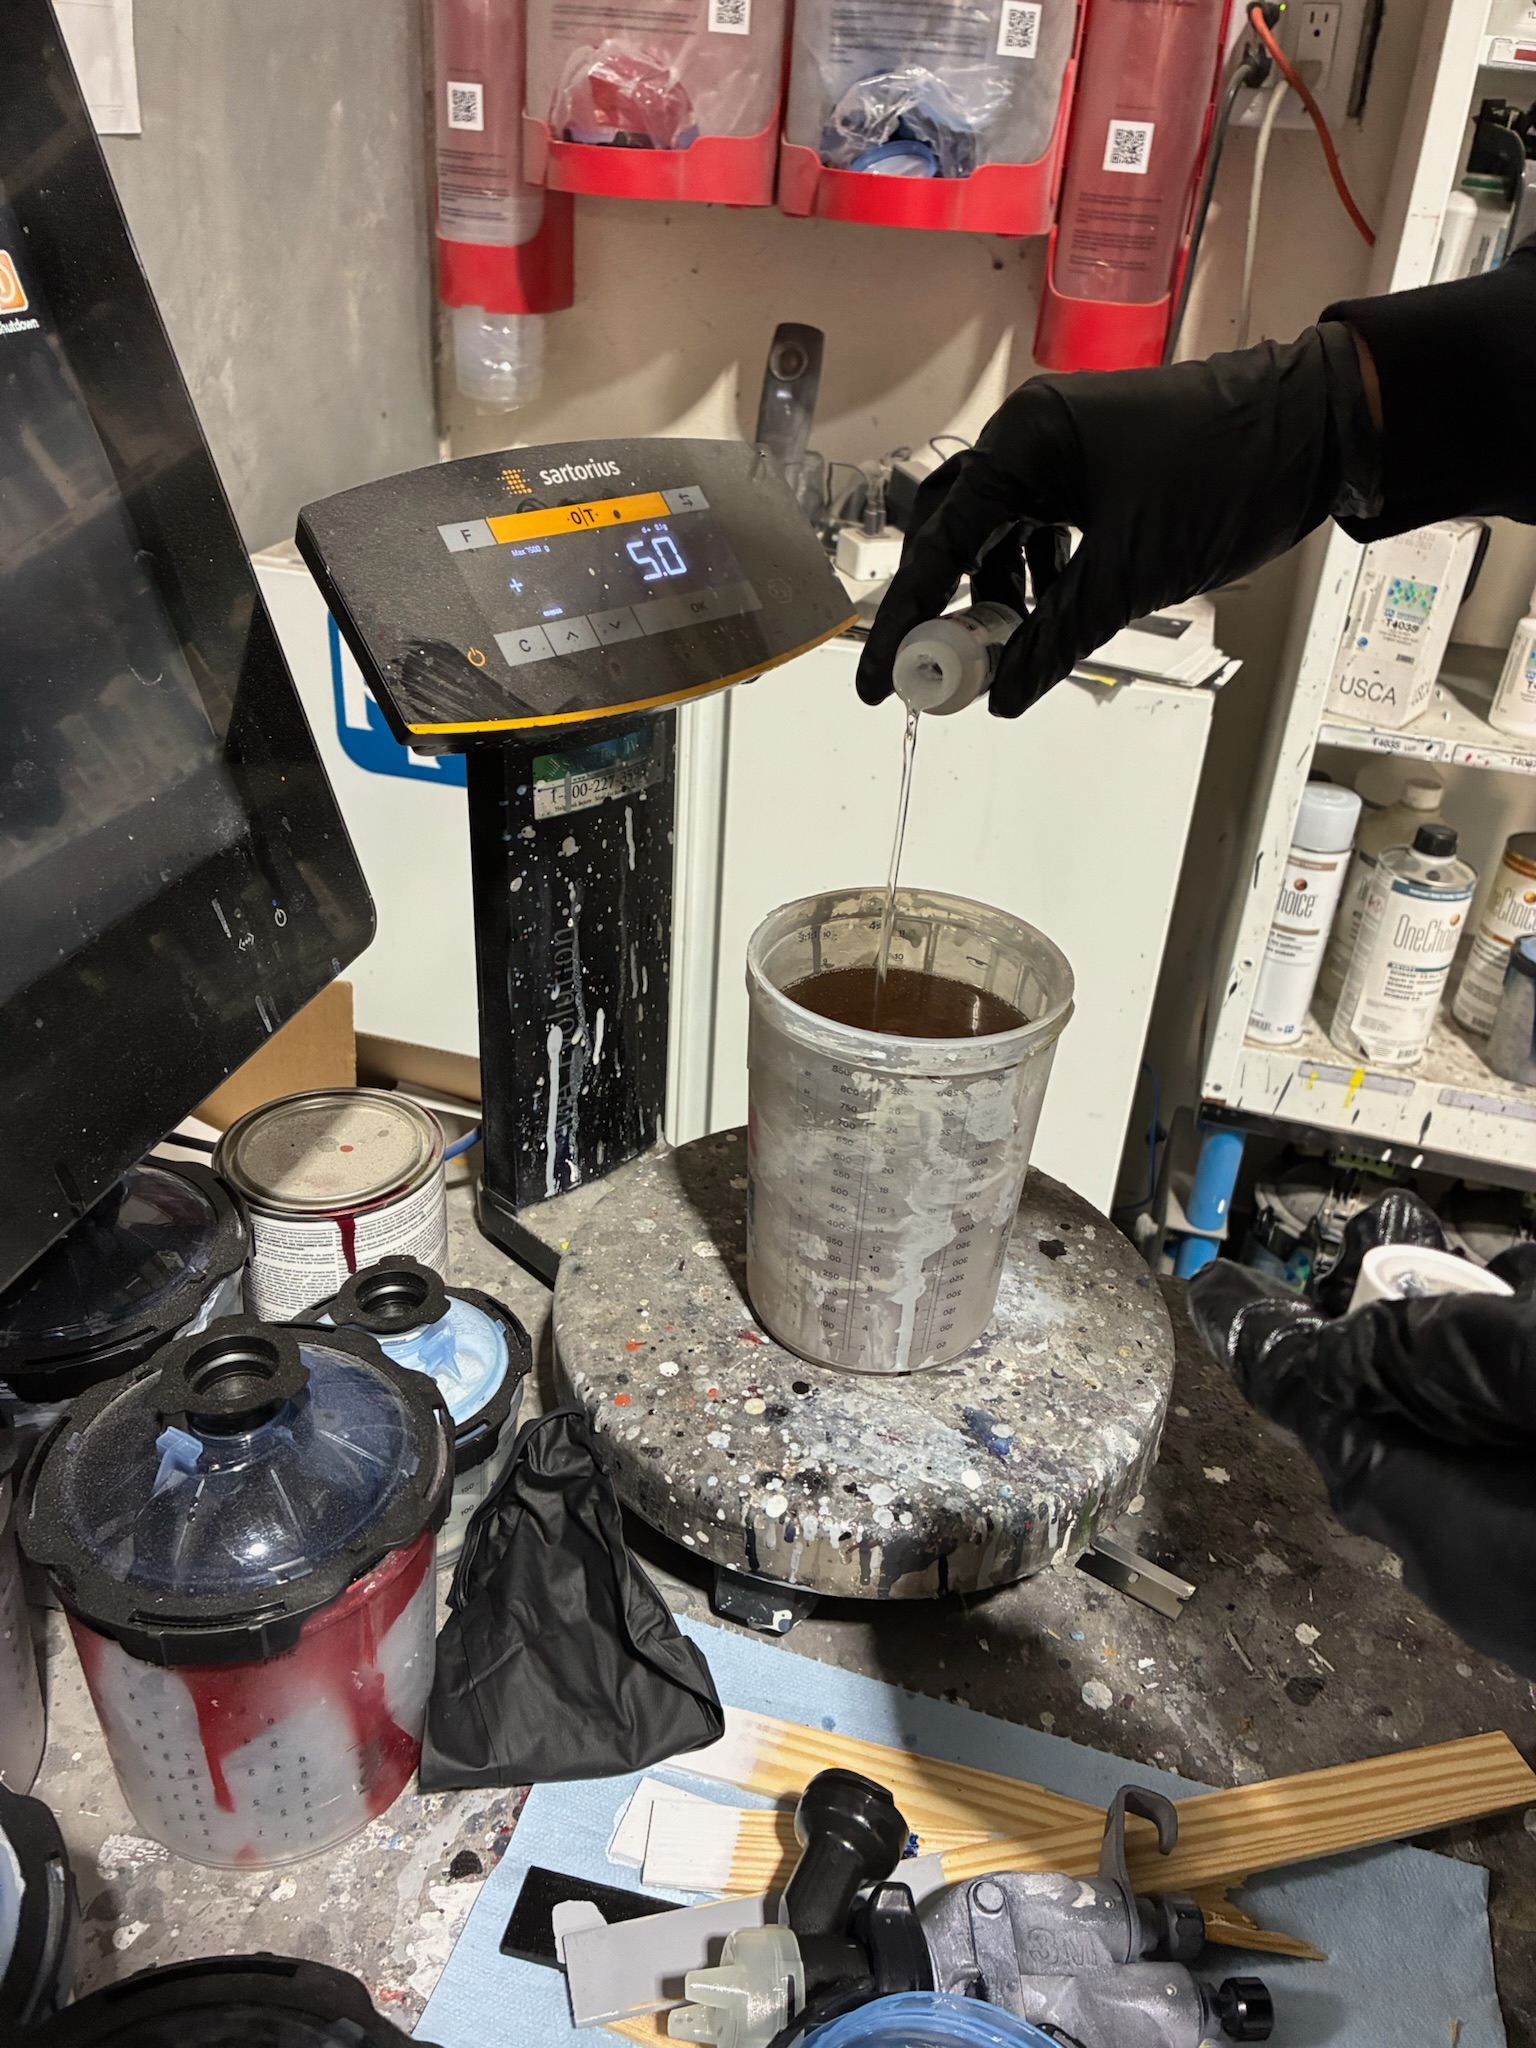
\includegraphics[
        width=2.35in,
        height=1.40in,
        keepaspectratio
    ]{spray_topcoat_prep}
};
\draw[RuleGray,line width=0.55pt,rounded corners=4pt]
    ($(current page.north west)+(0.43in,-1.91in)$)
    rectangle
    ($(current page.north west)+(2.98in,-3.40in)$);

% Image 2
\node[anchor=center,inner sep=0pt]
at ($(current page.north west)+(4.375in,-2.655in)$)
{
    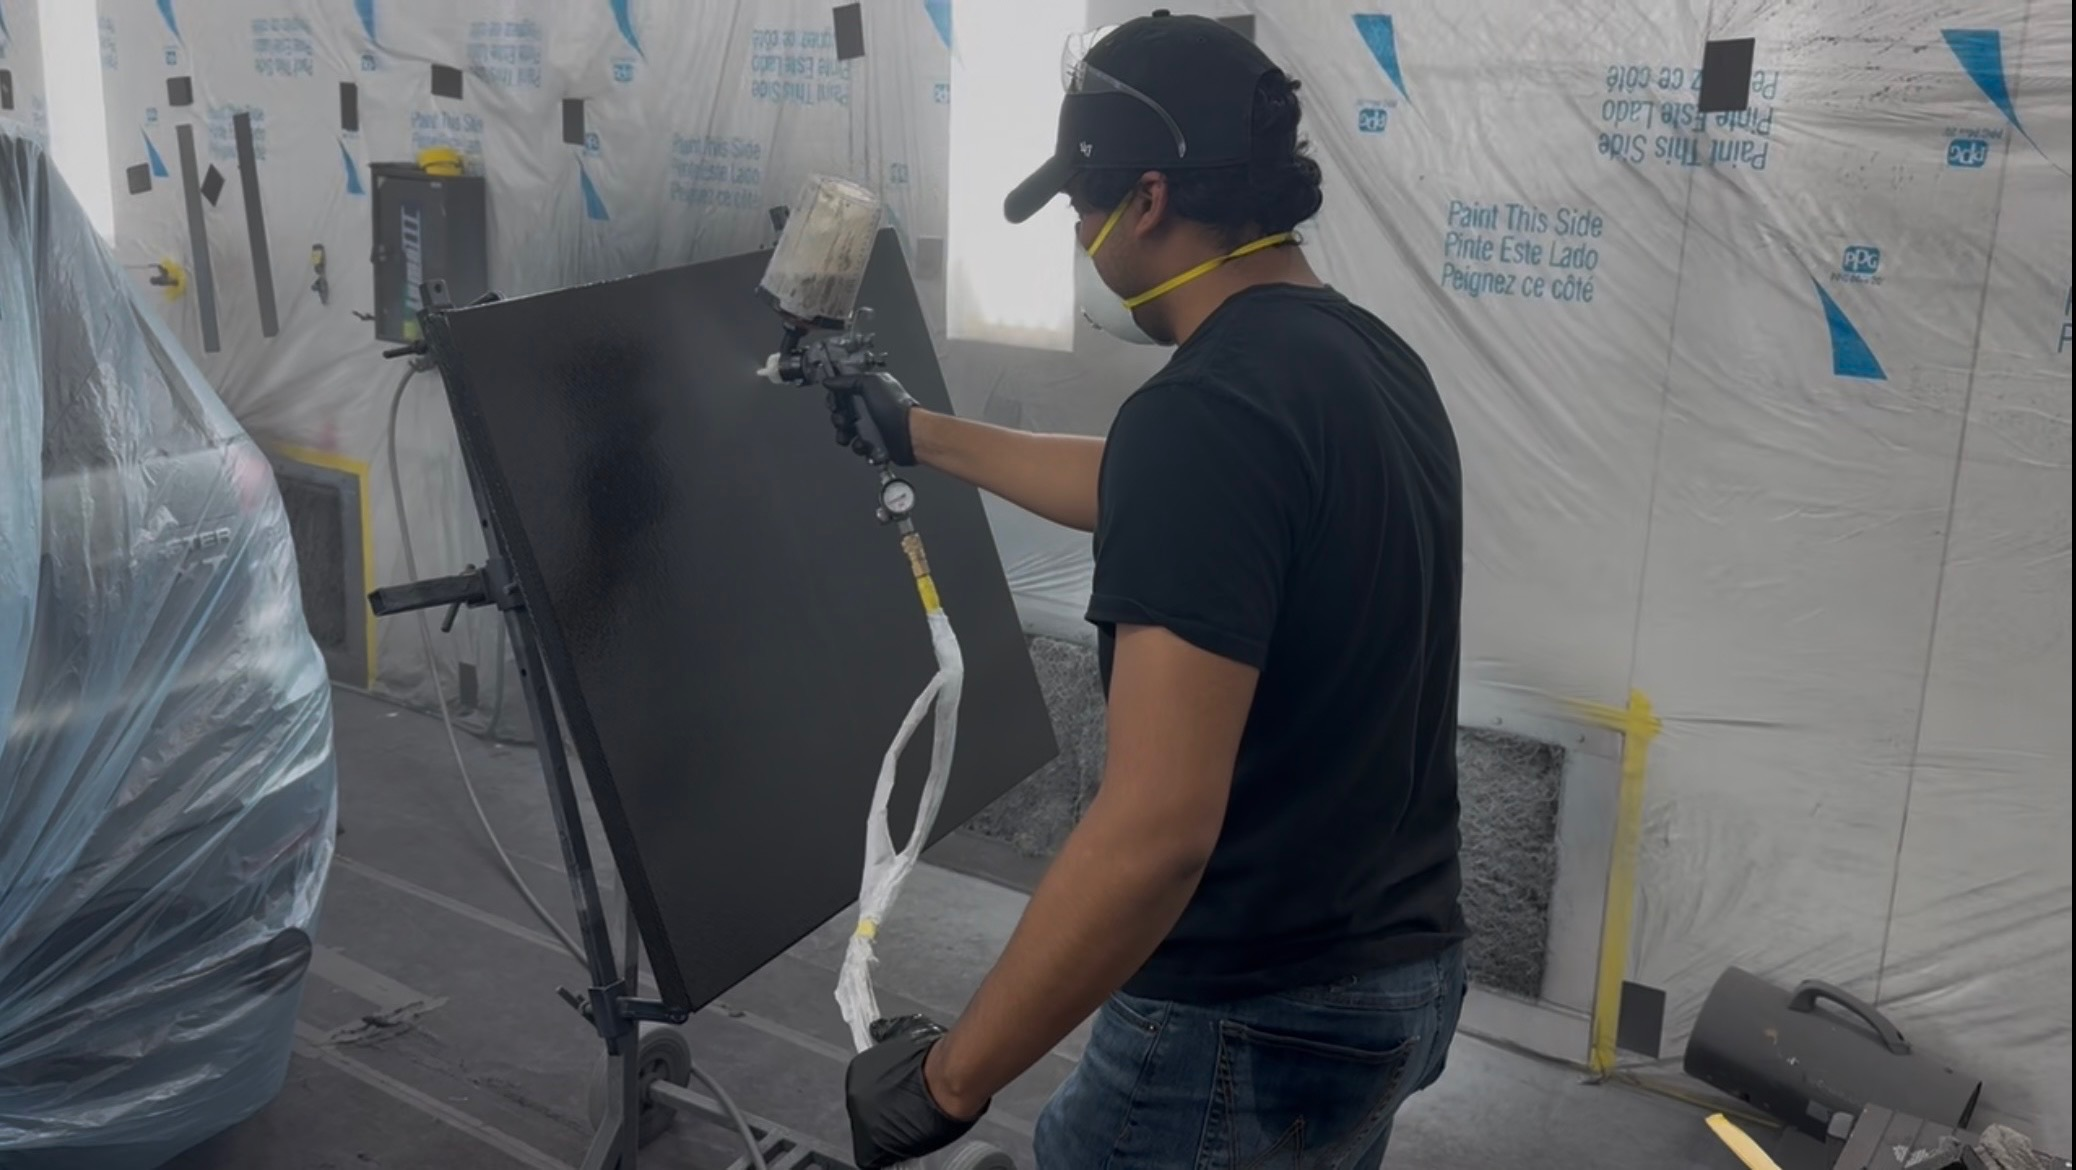
\includegraphics[
        width=2.35in,
        height=1.40in,
        keepaspectratio
    ]{spraying_topcoat}
};
\draw[RuleGray,line width=0.55pt,rounded corners=4pt]
    ($(current page.north west)+(3.10in,-1.91in)$)
    rectangle
    ($(current page.north west)+(5.65in,-3.40in)$);

% Image 3
\node[anchor=center,inner sep=0pt]
at ($(current page.north west)+(7.045in,-2.655in)$)
{
    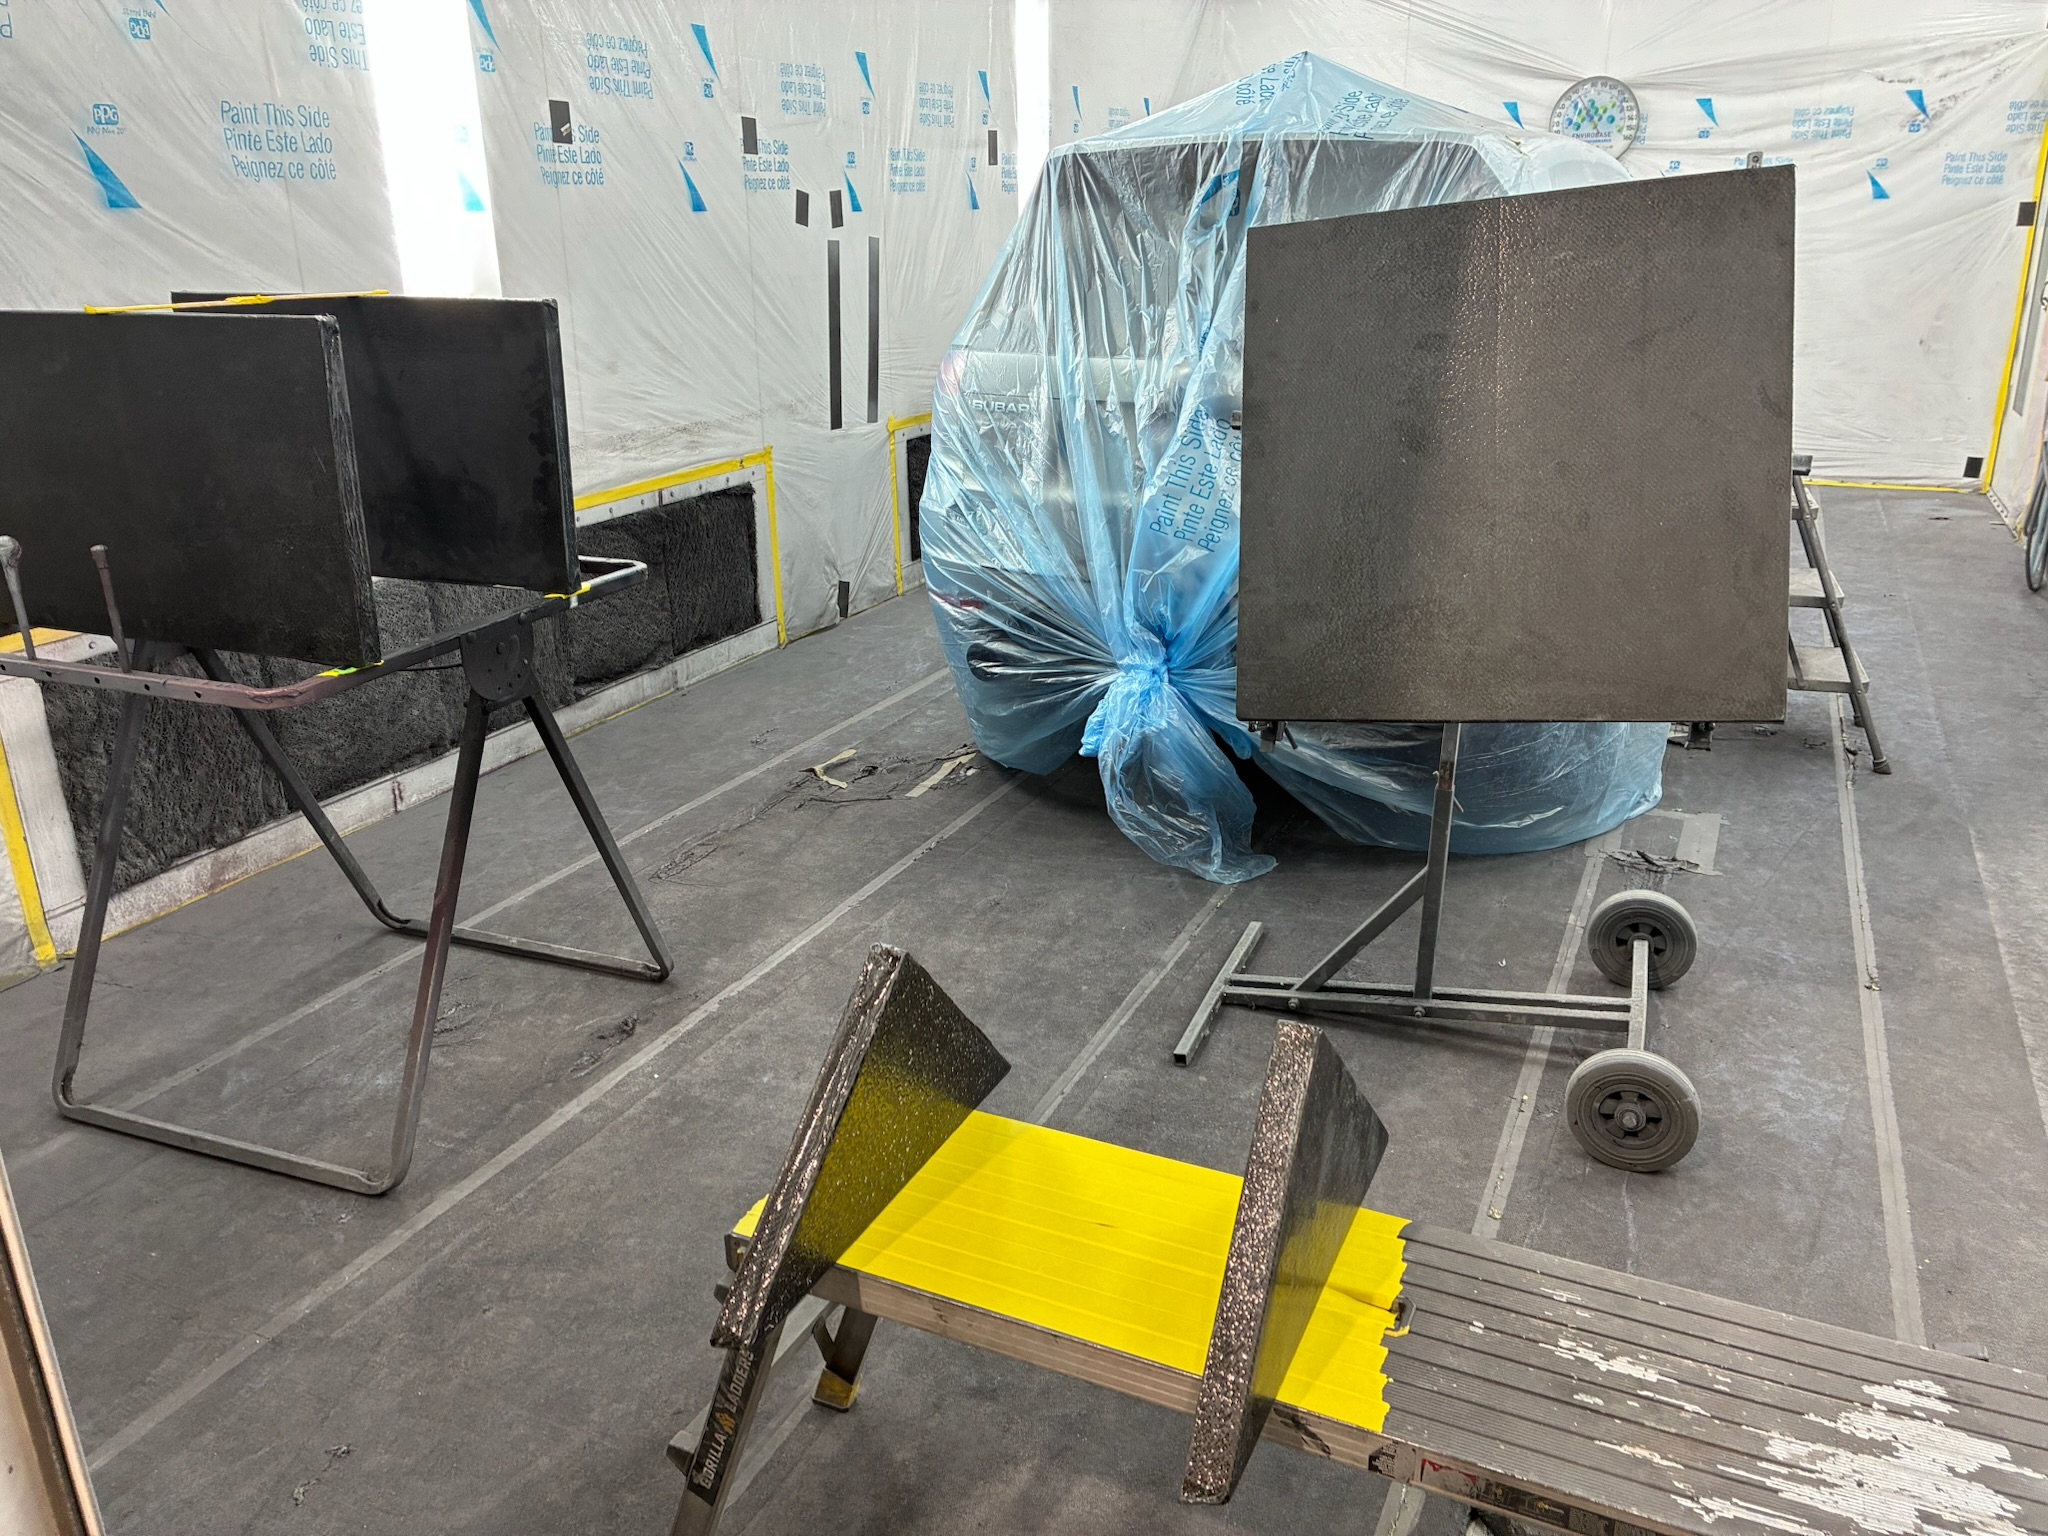
\includegraphics[
        width=2.35in,
        height=1.40in,
        keepaspectratio
    ]{topcoat_setup_apparatus}
};
\draw[RuleGray,line width=0.55pt,rounded corners=4pt]
    ($(current page.north west)+(5.77in,-1.91in)$)
    rectangle
    ($(current page.north west)+(8.32in,-3.40in)$);

% Image 4
\node[anchor=center,inner sep=0pt]
at ($(current page.north west)+(9.50in,-2.655in)$)
{
    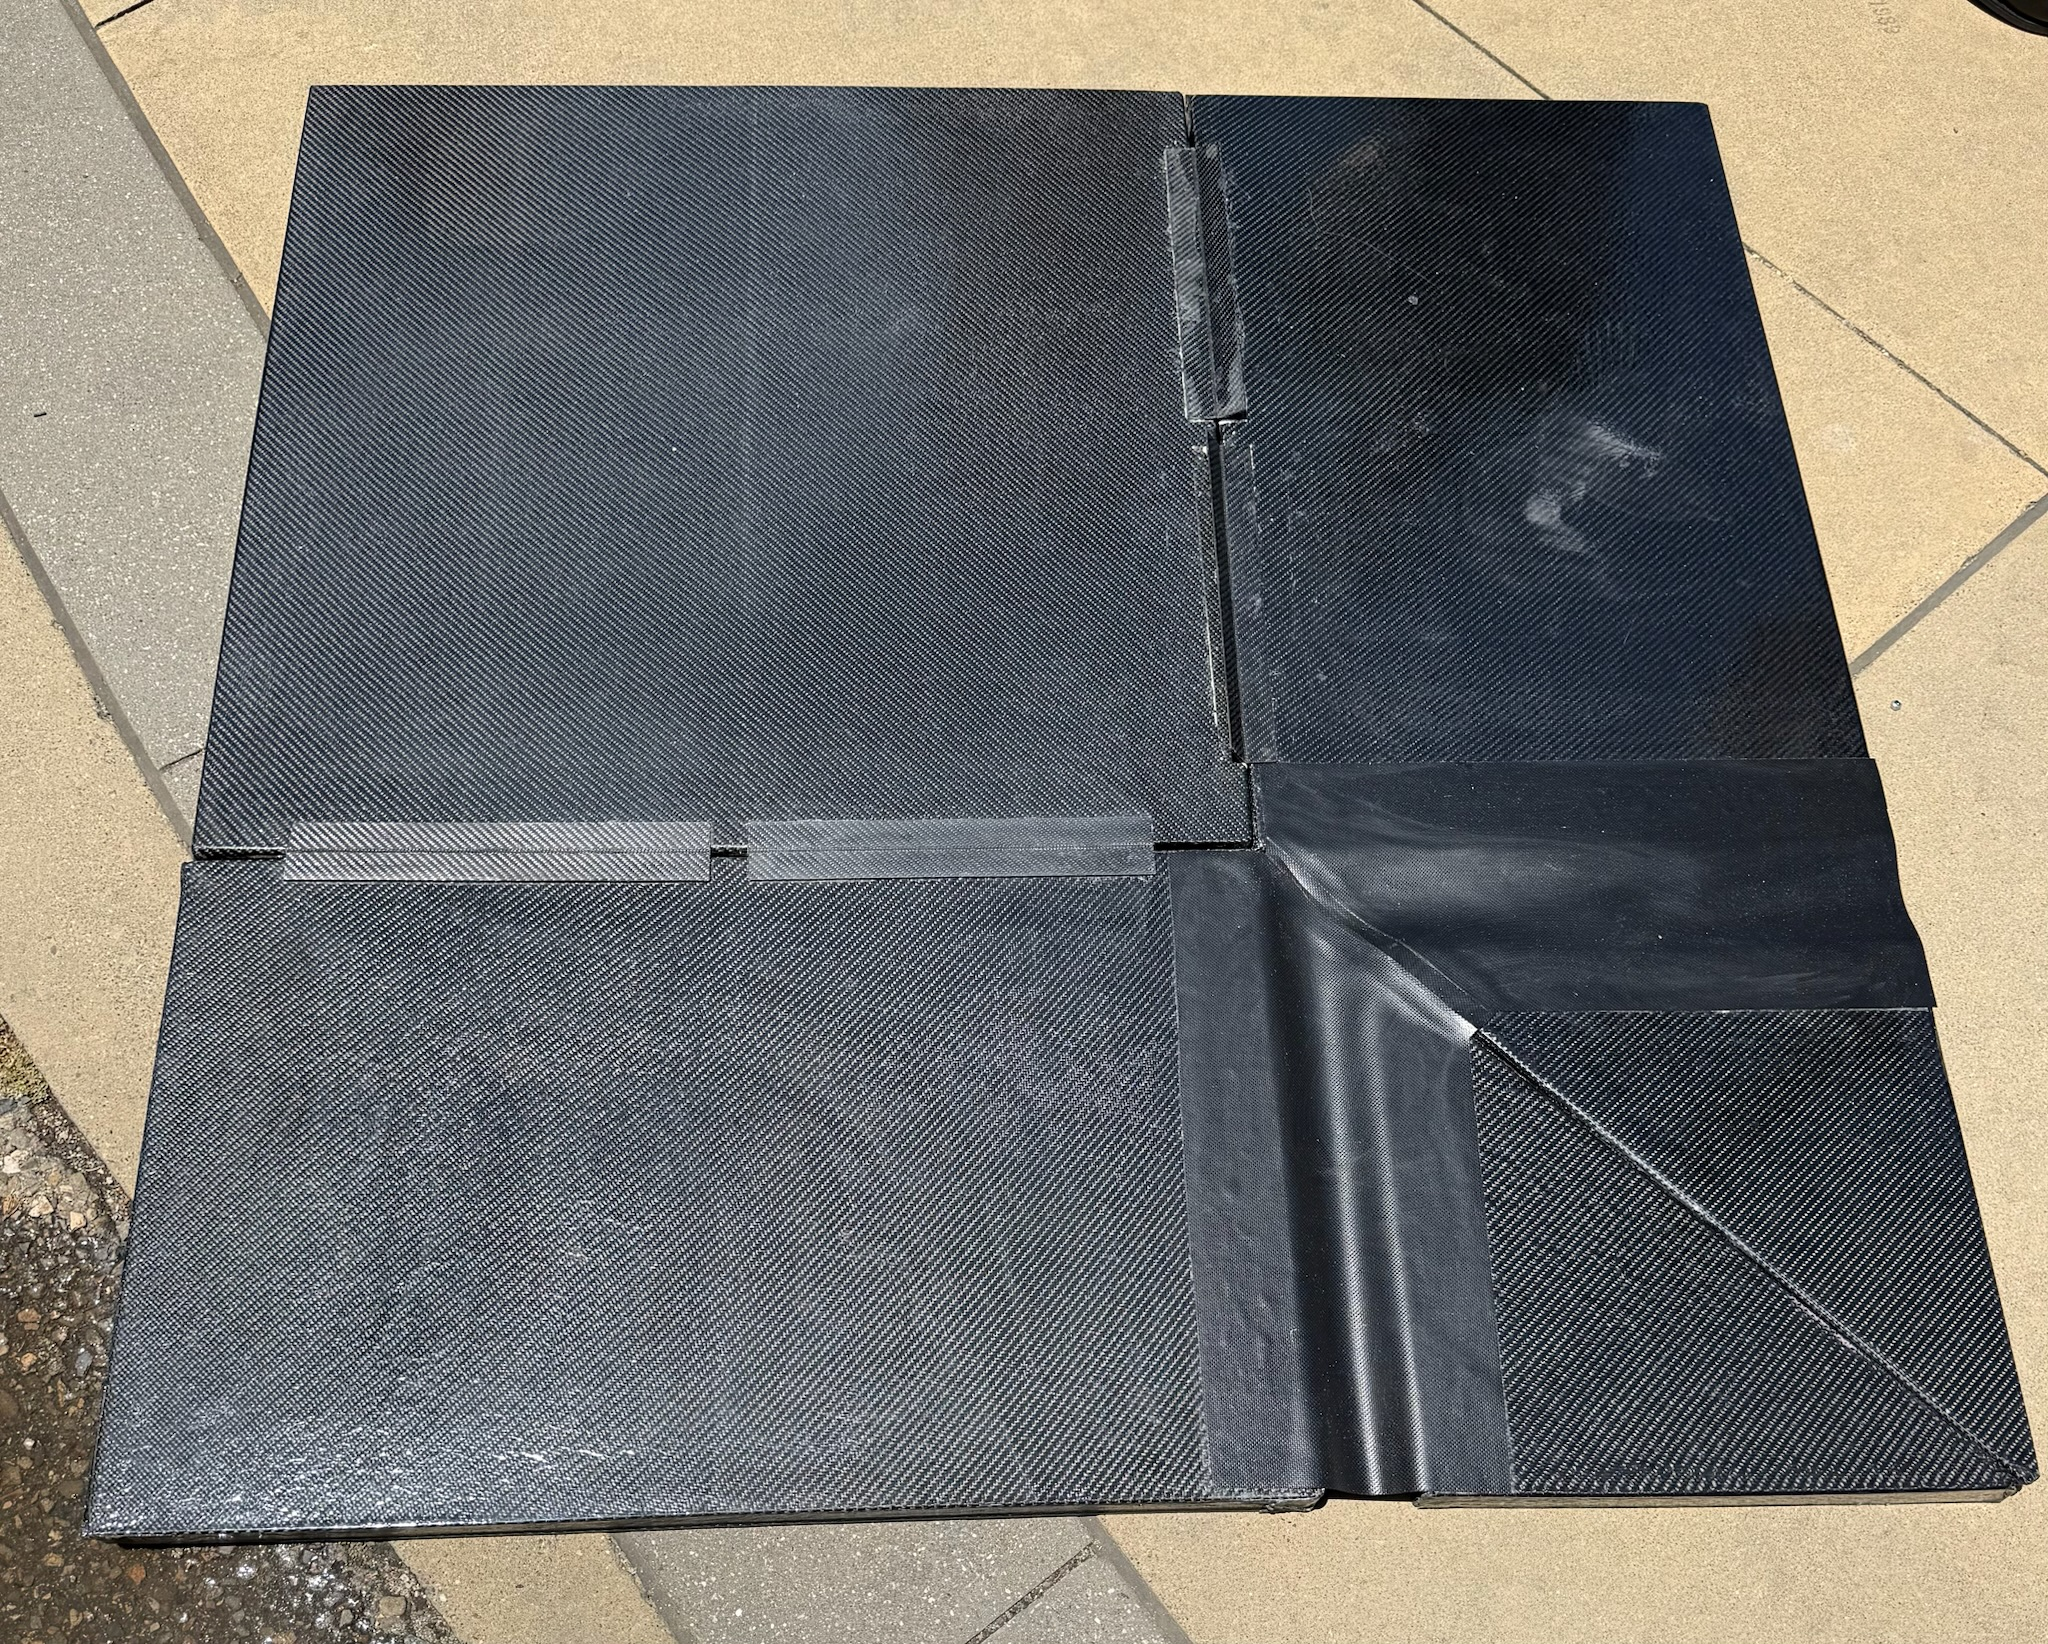
\includegraphics[
        width=2.35in,
        height=1.40in,
        keepaspectratio
    ]{refined_final_toro_cover_partial_carbon_model}
};
\draw[RuleGray,line width=0.55pt,rounded corners=4pt]
    ($(current page.north west)+(8.44in,-1.91in)$)
    rectangle
    ($(current page.north east)+(-0.42in,-3.40in)$);

% Captions
\node[anchor=north,text=Muted,font=\sffamily\fontsize{6.7}{7.3}\selectfont]
at ($(current page.north west)+(1.705in,-3.45in)$)
{Topcoat material preparation};

\node[anchor=north,text=Muted,font=\sffamily\fontsize{6.7}{7.3}\selectfont]
at ($(current page.north west)+(4.375in,-3.45in)$)
{Automotive-booth topcoat application};

\node[anchor=north,text=Muted,font=\sffamily\fontsize{6.7}{7.3}\selectfont]
at ($(current page.north west)+(7.045in,-3.45in)$)
{Coated panels drying after application};

\node[anchor=north,text=Muted,font=\sffamily\fontsize{6.7}{7.3}\selectfont]
at ($(current page.north west)+(9.50in,-3.45in)$)
{Partial carbon manufacturing model};

% Environmental rationale
\fill[SoftGold,rounded corners=4pt]
    ($(current page.north west)+(0.43in,-3.73in)$)
    rectangle
    ($(current page.north east)+(-0.42in,-4.76in)$);

\node[
    anchor=north west,
    align=left,
    text width=9.75in,
    text=Ink,
    font=\fontsize{7.05}{8.25}\selectfont
]
at ($(current page.north west)+(0.65in,-3.89in)$)
{
Because the sponsor required a carbon-fiber cover for outdoor use near chlorinated water,
environmental protection became a functional requirement rather than a cosmetic finish.
I selected and personally sprayed a UV-resistant Sunshield topcoat to seal minor laminate
porosity, reduce moisture ingress, preserve the carbon appearance, limit UV degradation of
the epoxy matrix, and isolate the composite surface from nearby metallic hardware.
};

% Results title
\node[
    anchor=north west,
    text=DeepGreen,
    font=\sffamily\bfseries\fontsize{8.0}{8.7}\selectfont
]
at ($(current page.north west)+(0.43in,-4.94in)$)
{FUNCTIONAL PROTOTYPE RESULTS};

% ------------------------------------------------------------
% Matched lower panels — larger type and improved allocation
% ------------------------------------------------------------

% Left results panel
\fill[SoftGreen,rounded corners=5pt]
    ($(current page.north west)+(0.43in,-5.22in)$)
    rectangle
    ($(current page.north west)+(5.98in,-7.39in)$);

\draw[RuleGray,line width=0.65pt,rounded corners=5pt]
    ($(current page.north west)+(0.43in,-5.22in)$)
    rectangle
    ($(current page.north west)+(5.98in,-7.39in)$);

\fill[DeepGreen,rounded corners=5pt]
    ($(current page.north west)+(0.43in,-5.22in)$)
    rectangle
    ($(current page.north west)+(5.98in,-5.58in)$);

\fill[DeepGreen]
    ($(current page.north west)+(0.43in,-5.40in)$)
    rectangle
    ($(current page.north west)+(5.98in,-5.58in)$);

\node[anchor=west,text=white,
      font=\sffamily\bfseries\fontsize{7.0}{7.6}\selectfont]
at ($(current page.north west)+(0.66in,-5.40in)$)
{SPECIFICATION};

\node[anchor=west,text=white,
      font=\sffamily\bfseries\fontsize{7.0}{7.6}\selectfont]
at ($(current page.north west)+(3.02in,-5.40in)$)
{RESULT};

\node[anchor=east,text=white,
      font=\sffamily\bfseries\fontsize{7.0}{7.6}\selectfont]
at ($(current page.north west)+(5.55in,-5.40in)$)
{STATUS};

\node[
    anchor=north west,
    align=left,
    text width=2.15in,
    text=Ink,
    font=\bfseries\fontsize{7.15}{8.55}\selectfont
]
at ($(current page.north west)+(0.66in,-5.72in)$)
{
Deployment time\\[3.4pt]
Removal time\\[3.4pt]
Single-user operation\\[3.4pt]
Single-side operation\\[3.4pt]
Deployment steps\\[3.4pt]
Removal steps\\[3.4pt]
Weight\\[3.4pt]
Folded storage
};

\node[
    anchor=north west,
    align=left,
    text width=1.45in,
    text=Ink,
    font=\fontsize{7.15}{8.55}\selectfont
]
at ($(current page.north west)+(3.02in,-5.72in)$)
{
25.51 seconds\\[3.4pt]
37.22 seconds\\[3.4pt]
100\% successful\\[3.4pt]
75\% successful\\[3.4pt]
6.4 average\\[3.4pt]
9 average\\[3.4pt]
17 lb\\[3.4pt]
2.9' x 2.9' x 1.7'
};

\node[
    anchor=north east,
    align=right,
    text width=1.05in,
    text=DeepGreen,
    font=\sffamily\bfseries\fontsize{7.05}{8.55}\selectfont
]
at ($(current page.north west)+(5.55in,-5.72in)$)
{
PASS\\[3.4pt]
PASS\\[3.4pt]
PASS\\[3.4pt]
NEAR TARGET\\[3.4pt]
PASS\\[3.4pt]
PASS\\[3.4pt]
NEAR TARGET\\[3.4pt]
PASS
};

% Right takeaways panel — widened for easier reading
\fill[SoftGreen,rounded corners=5pt]
    ($(current page.north west)+(6.14in,-5.22in)$)
    rectangle
    ($(current page.north east)+(-0.42in,-7.39in)$);

\draw[RuleGray,line width=0.65pt,rounded corners=5pt]
    ($(current page.north west)+(6.14in,-5.22in)$)
    rectangle
    ($(current page.north east)+(-0.42in,-7.39in)$);

\fill[DeepGreen,rounded corners=5pt]
    ($(current page.north west)+(6.14in,-5.22in)$)
    rectangle
    ($(current page.north east)+(-0.42in,-5.58in)$);

\fill[DeepGreen]
    ($(current page.north west)+(6.14in,-5.40in)$)
    rectangle
    ($(current page.north east)+(-0.42in,-5.58in)$);

\node[anchor=west,text=white,
      font=\sffamily\bfseries\fontsize{7.1}{7.7}\selectfont]
at ($(current page.north west)+(6.38in,-5.40in)$)
{ENGINEERING TAKEAWAYS};

\node[
    anchor=north west,
    align=left,
    text width=4.02in,
    text=Ink,
    font=\fontsize{6.75}{7.85}\selectfont
]
at ($(current page.north west)+(6.38in,-5.72in)$)
{
\textbf{Manufacturing first.}
Composite manufacturing constraints should guide the product architecture from the beginning.\\[4.5pt]
\textbf{Prioritize deliberately.}
Competing requirements must be balanced intentionally instead of maximizing every objective.\\[4.5pt]
\textbf{Lead through the process.}
Clear procedures, calm communication, and respect for teammates' strengths were essential during fabrication.\\[4.5pt]
\textbf{Next iteration.}
Reduce weight, refine the fabric-hinge fold lines, and improve panel-edge clearance.
};

% Compact concluding pathway
\node[
    anchor=center,
    align=center,
    text=PolyGold,
    font=\sffamily\bfseries\fontsize{6.3}{6.9}\selectfont
]
at ($(current page.north)+(3.06in,-7.18in)$)
{PROTOTYPE \faArrowRight\ DESIGN REFINEMENT
\faArrowRight\ REPEATABLE MANUFACTURING
\faArrowRight\ PRODUCT};

% Validation resources
\node[
    anchor=north,
    align=center,
    text=DeepGreen,
    font=\sffamily\bfseries\fontsize{6.6}{7.2}\selectfont
]
at ($(current page.north)+(0,-7.58in)$)
{\href{\ToroDeploymentLink}{\faPlayCircle\ DEPLOYMENT}
\hspace{18pt}
\href{\ToroRemovalLink}{\faPlayCircle\ REMOVAL / FOLDING}
\hspace{18pt}
\href{\ToroPosterLink}{\faFilePdf\ EXPO POSTER}
\hspace{18pt}
\href{\ToroReportLink}{\faFilePdf\ FINAL REPORT}};

% Footer
\node[
    anchor=south west,
    text=white,
    font=\sffamily\bfseries\fontsize{7.1}{7.7}\selectfont
]
at ($(current page.south west)+(0.42in,0.17in)$)
{\faArrowLeft\ MANUFACTURING-DRIVEN DESIGN};

\node[
    anchor=south,
    text=white,
    font=\sffamily\fontsize{7.0}{7.6}\selectfont
]
at ($(current page.south)+(0,0.17in)$)
{TORO COVER \hspace{6pt} 3 / 3};

\node[
    anchor=south east,
    text=white,
    font=\sffamily\bfseries\fontsize{7.1}{7.7}\selectfont
]
at ($(current page.south east)+(-0.42in,0.17in)$)
{NEXT PROJECT \faArrowRight};

\end{tikzpicture}
\input{paddle}
\clearpage
.
% 2. In main.tex, place 
% ============================================================
% TORO COVER — THREE-PAGE PORTFOLIO CASE STUDY
% Pages 3–5 of the complete portfolio
%
% IMPORTANT:
% 1. This file must NOT contain \documentclass, \begin{document},
%    \end{document}, or \input{toro}.
% 2. In main.tex, place \input{toro} before \end{document}.
% 3. Image references use the original Overleaf base filenames
%    without extensions.
% ============================================================



% ============================================================
% CLICKABLE PROJECT RESOURCES
% All links use the exact Google Drive resources supplied.
% ============================================================
\providecommand{\ToroDrawingLink}{https://drive.google.com/file/d/1A7-7wMnRNLuQDaTgxeuUCBsGNqyXzOGV/view?usp=sharing}
\providecommand{\ToroDimensionsLink}{https://drive.google.com/file/d/13sw3BNJvE8GdzlRffxoF2n5r9Gzxide7/view?usp=sharing}
\providecommand{\ToroProblemLink}{https://drive.google.com/file/d/1zHtl8zrb13F1yeN74ptawpfS5UM_xsuw/view?usp=drive_link}
\providecommand{\ToroReportLink}{https://drive.google.com/file/d/1ULZ-P46lFsC2x29ZfmRVIKgYnr9o8hMt/view?usp=drive_link}
\providecommand{\ToroPosterLink}{https://drive.google.com/file/d/1vKiKaJUcHQb_db-FkZnRF6EvtuM4hKyS/view?usp=drive_link}
\providecommand{\ToroDeploymentLink}{https://drive.google.com/file/d/1XJx34o80_mZPTl7xy93HtWAgtS3ThhvY/view?usp=drive_link}
\providecommand{\ToroRemovalLink}{https://drive.google.com/file/d/1O7xYeyB67NUwT-j1B1HeiCcHnZDYjk6_/view?usp=drive_link}

% ============================================================
% PAGE 1 — PROJECT OVERVIEW, OWNERSHIP, AND ARCHITECTURE
% ============================================================

\clearpage
\thispagestyle{empty}
\hypertarget{toro}{}
\null

\begin{tikzpicture}[remember picture,overlay]

% Background
\fill[white]
    (current page.south west)
    rectangle
    (current page.north east);

% Page bars
\fill[DeepGreen]
    (current page.north west)
    rectangle
    ($(current page.north east)+(0,-0.095in)$);

\fill[PolyGold]
    ($(current page.north west)+(0,-0.095in)$)
    rectangle
    ($(current page.north east)+(0,-0.14in)$);

\fill[DeepGreen]
    (current page.south west)
    rectangle
    ($(current page.south east)+(0,0.36in)$);

\fill[PolyGold]
    ($(current page.south west)+(0,0.36in)$)
    rectangle
    ($(current page.south east)+(0,0.405in)$);

% Header
\node[
    anchor=north west,
    text=PolyGold,
    font=\sffamily\bfseries\fontsize{8.1}{8.7}\selectfont
]
at ($(current page.north west)+(0.42in,-0.39in)$)
{01 COMPOSITES \hspace{5pt}/\hspace{5pt} PROJECT 01};

\node[
    anchor=north west,
    text=DeepGreen,
    font=\bfseries\fontsize{23.5}{24.5}\selectfont
]
at ($(current page.north west)+(0.40in,-0.67in)$)
{TORO CARBON FIBER SAFETY COVER};

\node[
    anchor=north west,
    text=Muted,
    font=\sffamily\fontsize{8.4}{9.2}\selectfont
]
at ($(current page.north west)+(0.42in,-1.12in)$)
{Cal Poly Composites Laboratory \hspace{7pt}\textbullet\hspace{7pt}
Team Project \hspace{7pt}\textbullet\hspace{7pt}
Fall--Spring 2026 \hspace{7pt}\textbullet\hspace{7pt}
San Luis Obispo, California};

\fill[PolyGold]
    ($(current page.north west)+(0.42in,-1.37in)$)
    rectangle
    ($(current page.north west)+(6.1in,-1.325in)$);

% Challenge text
\node[
    anchor=north west,
    text=DeepGreen,
    font=\sffamily\bfseries\fontsize{8.1}{8.8}\selectfont
]
at ($(current page.north west)+(0.43in,-1.61in)$)
{THE CHALLENGE};

\node[
    anchor=north west,
    align=left,
    text width=4.47in,
    text=Ink,
    font=\fontsize{8.05}{9.65}\selectfont
]
at ($(current page.north west)+(0.43in,-1.84in)$)
{
Develop a lightweight cover for a 6 ft by 6 ft in-ground spa
that could be deployed by one person, stored compactly,
provide insulation, resist a poolside environment, and maintain
a refined appearance. The sponsor supplied an ambitious but
intentionally broad project statement, requiring the team to
define the product architecture, priorities, manufacturing
strategy, and realistic path toward future commercialization.
};

% Role box
\fill[SoftGold,rounded corners=5pt]
    ($(current page.north west)+(0.42in,-2.88in)$)
    rectangle
    ($(current page.north west)+(4.98in,-4.58in)$);

\fill[PolyGold]
    ($(current page.north west)+(0.42in,-2.88in)$)
    rectangle
    ($(current page.north west)+(0.52in,-4.58in)$);

\node[
    anchor=north west,
    text=DeepGreen,
    font=\sffamily\bfseries\fontsize{8.1}{8.8}\selectfont
]
at ($(current page.north west)+(0.66in,-3.02in)$)
{MY ROLE — DESIGN \& MANUFACTURING LEAD};

\node[
    anchor=north west,
    align=left,
    text width=4.02in,
    text=Ink,
    font=\fontsize{7.05}{8.15}\selectfont
]
at ($(current page.north west)+(0.66in,-3.27in)$)
{
\textbullet\ Modeled every custom part and the complete assembly\\[1.5pt]
\textbullet\ Produced the engineering drawing package independently\\[1.5pt]
\textbullet\ Developed the composite-panel manufacturing process\\[1.5pt]
\textbullet\ Created all waterjet DXFs and manufacturing geometry\\[1.5pt]
\textbullet\ Trained teammates in wet layup and vacuum bagging\\[1.5pt]
\textbullet\ Presented feasibility, scope, and tradeoffs to the sponsor
};

% Large deployed foam-model image
\node[anchor=center,inner sep=0pt]
at ($(current page.north west)+(8.00in,-3.04in)$)
{
    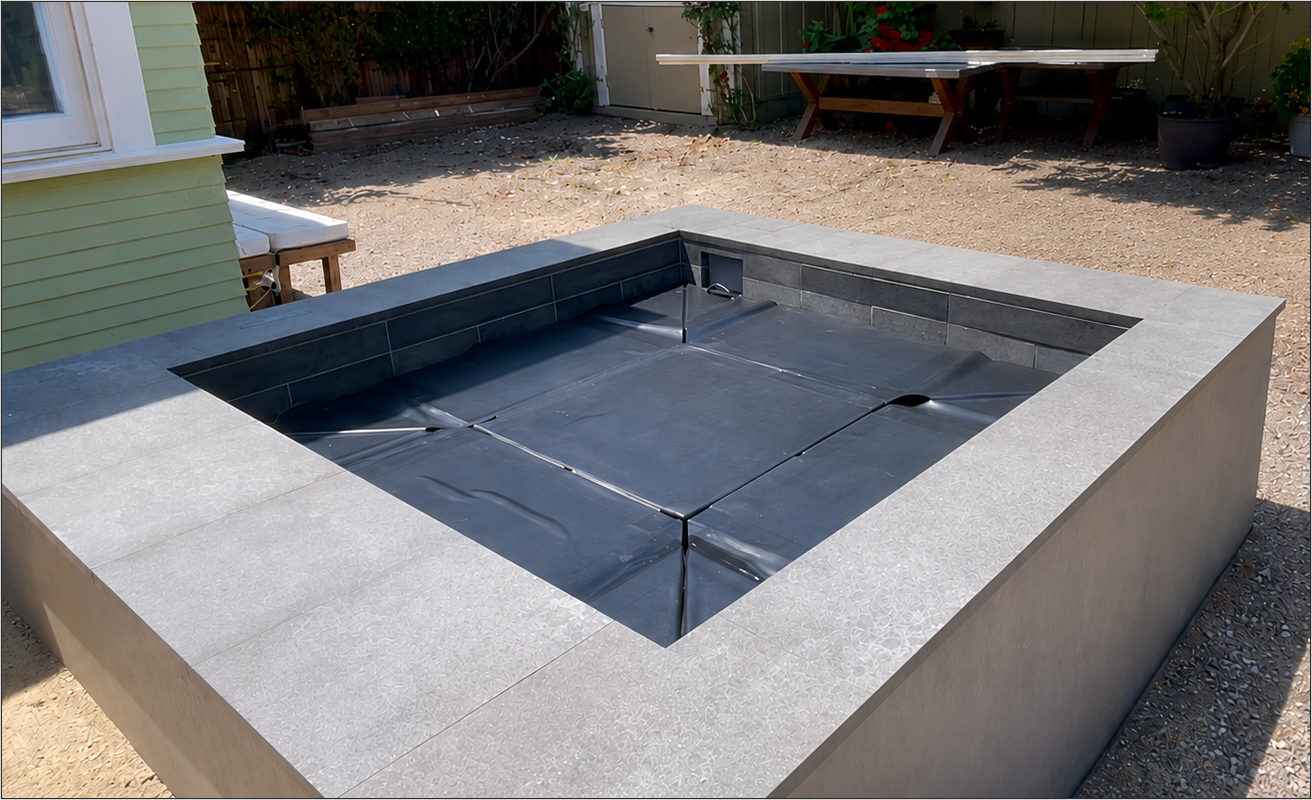
\includegraphics[
        width=5.55in,
        height=2.78in,
        keepaspectratio
    ]{deployed_functional_prototype}
};

\draw[DeepGreen,line width=0.8pt,rounded corners=7pt]
    ($(current page.north west)+(5.16in,-1.61in)$)
    rectangle
    ($(current page.north east)+(-0.42in,-4.47in)$);

\node[
    anchor=north west,
    text=Muted,
    font=\sffamily\fontsize{6.2}{6.9}\selectfont
]
at ($(current page.north west)+(5.18in,-4.54in)$)
{Functional foam model deployed over the sponsor's in-ground spa.};

% Image-strip title
\node[
    anchor=north west,
    text=DeepGreen,
    font=\sffamily\bfseries\fontsize{8.1}{8.8}\selectfont
]
at ($(current page.north west)+(0.43in,-4.78in)$)
{PRODUCT DEVELOPMENT AND FINAL ARCHITECTURE};

% Five-image development strip — CAD-first sequence
% Image 1: topside CAD
\node[anchor=center,inner sep=0pt]
at ($(current page.north west)+(1.47in,-5.73in)$)
{
    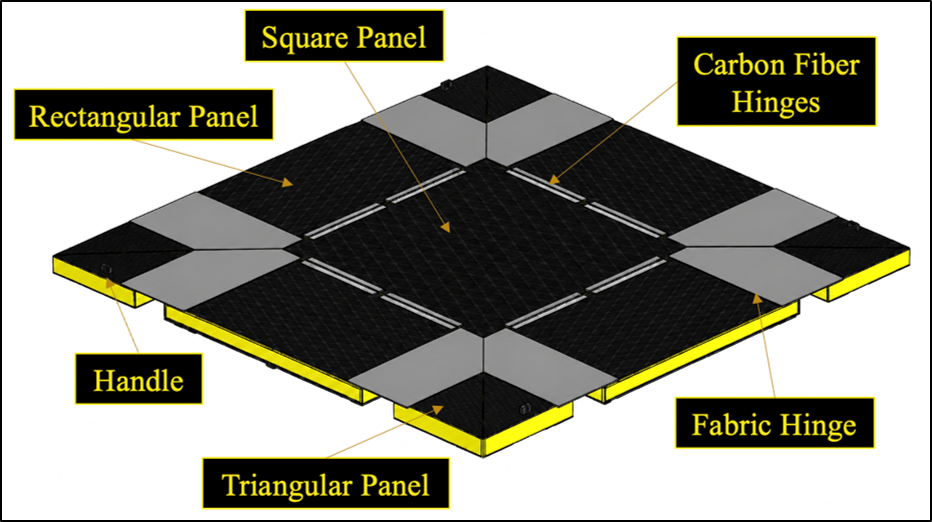
\includegraphics[
        width=1.92in,
        height=1.30in,
        keepaspectratio
    ]{Toro_Cover_topside_Cad}
};
\draw[RuleGray,line width=0.55pt,rounded corners=4pt]
    ($(current page.north west)+(0.43in,-5.04in)$)
    rectangle
    ($(current page.north west)+(2.51in,-6.43in)$);

% Image 2: underside CAD
\node[anchor=center,inner sep=0pt]
at ($(current page.north west)+(3.66in,-5.73in)$)
{
    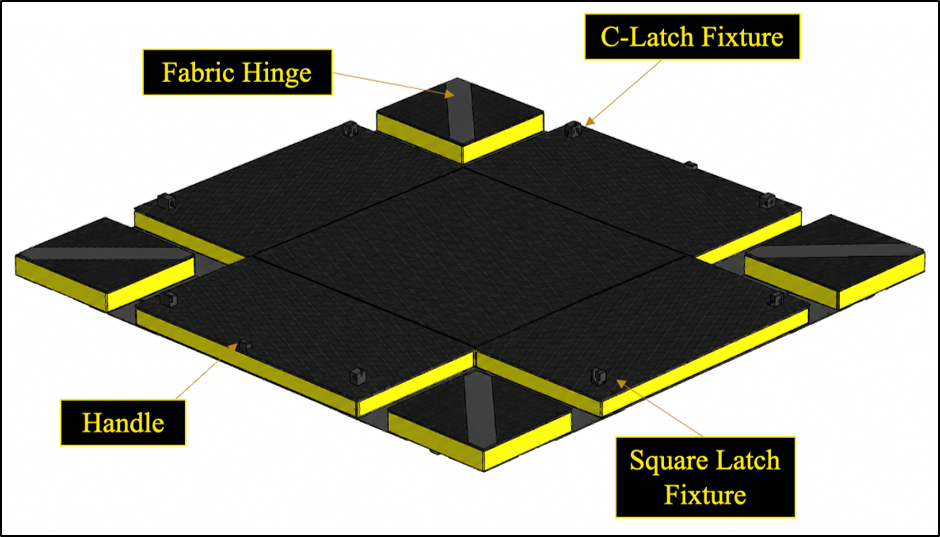
\includegraphics[
        width=1.92in,
        height=1.30in,
        keepaspectratio
    ]{toro_cover_underside_cad}
};
\draw[RuleGray,line width=0.55pt,rounded corners=4pt]
    ($(current page.north west)+(2.62in,-5.04in)$)
    rectangle
    ($(current page.north west)+(4.70in,-6.43in)$);

% Image 3: folded CAD
\node[anchor=center,inner sep=0pt]
at ($(current page.north west)+(5.85in,-5.73in)$)
{
    \includegraphics[
        width=1.92in,
        height=1.30in,
        keepaspectratio
    ]{\detokenize{Toro_Cover_folded Configuration}}
};
\draw[RuleGray,line width=0.55pt,rounded corners=4pt]
    ($(current page.north west)+(4.81in,-5.04in)$)
    rectangle
    ($(current page.north west)+(6.89in,-6.43in)$);

% Image 4: dual-use product concept
\node[anchor=center,inner sep=0pt]
at ($(current page.north west)+(8.04in,-5.73in)$)
{
    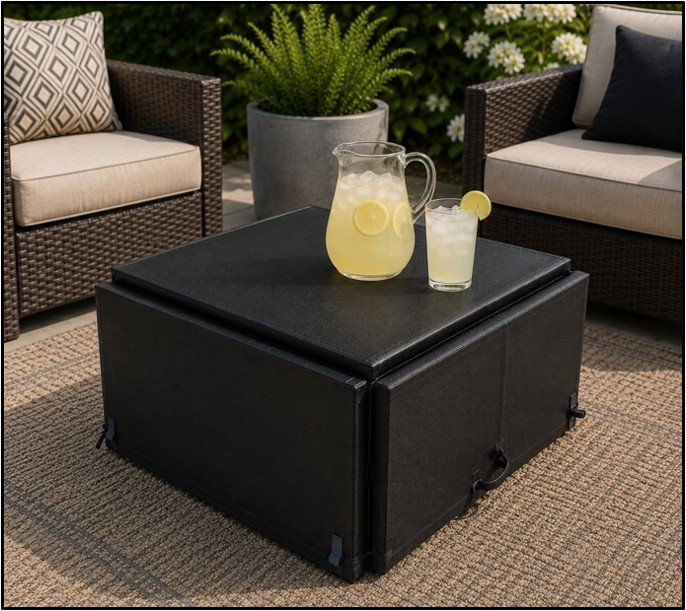
\includegraphics[
        width=1.92in,
        height=1.30in,
        keepaspectratio
    ]{generative_AI_concept_toro_cover_art}
};
\draw[RuleGray,line width=0.55pt,rounded corners=4pt]
    ($(current page.north west)+(7.00in,-5.04in)$)
    rectangle
    ($(current page.north west)+(9.08in,-6.43in)$);

% Image 5: folded foam functional prototype
% The portrait photograph is deliberately clipped to the landscape frame
% so the ottoman fills the card without extending beyond its border.
\begin{scope}
\clip[rounded corners=4pt]
    ($(current page.north west)+(9.19in,-5.04in)$)
    rectangle
    ($(current page.north east)+(-0.43in,-6.43in)$);

% Keep the original image proportions and center it within the existing card.
\node[anchor=center,inner sep=0pt]
at ($(current page.north west)+(9.88in,-5.735in)$)
{
    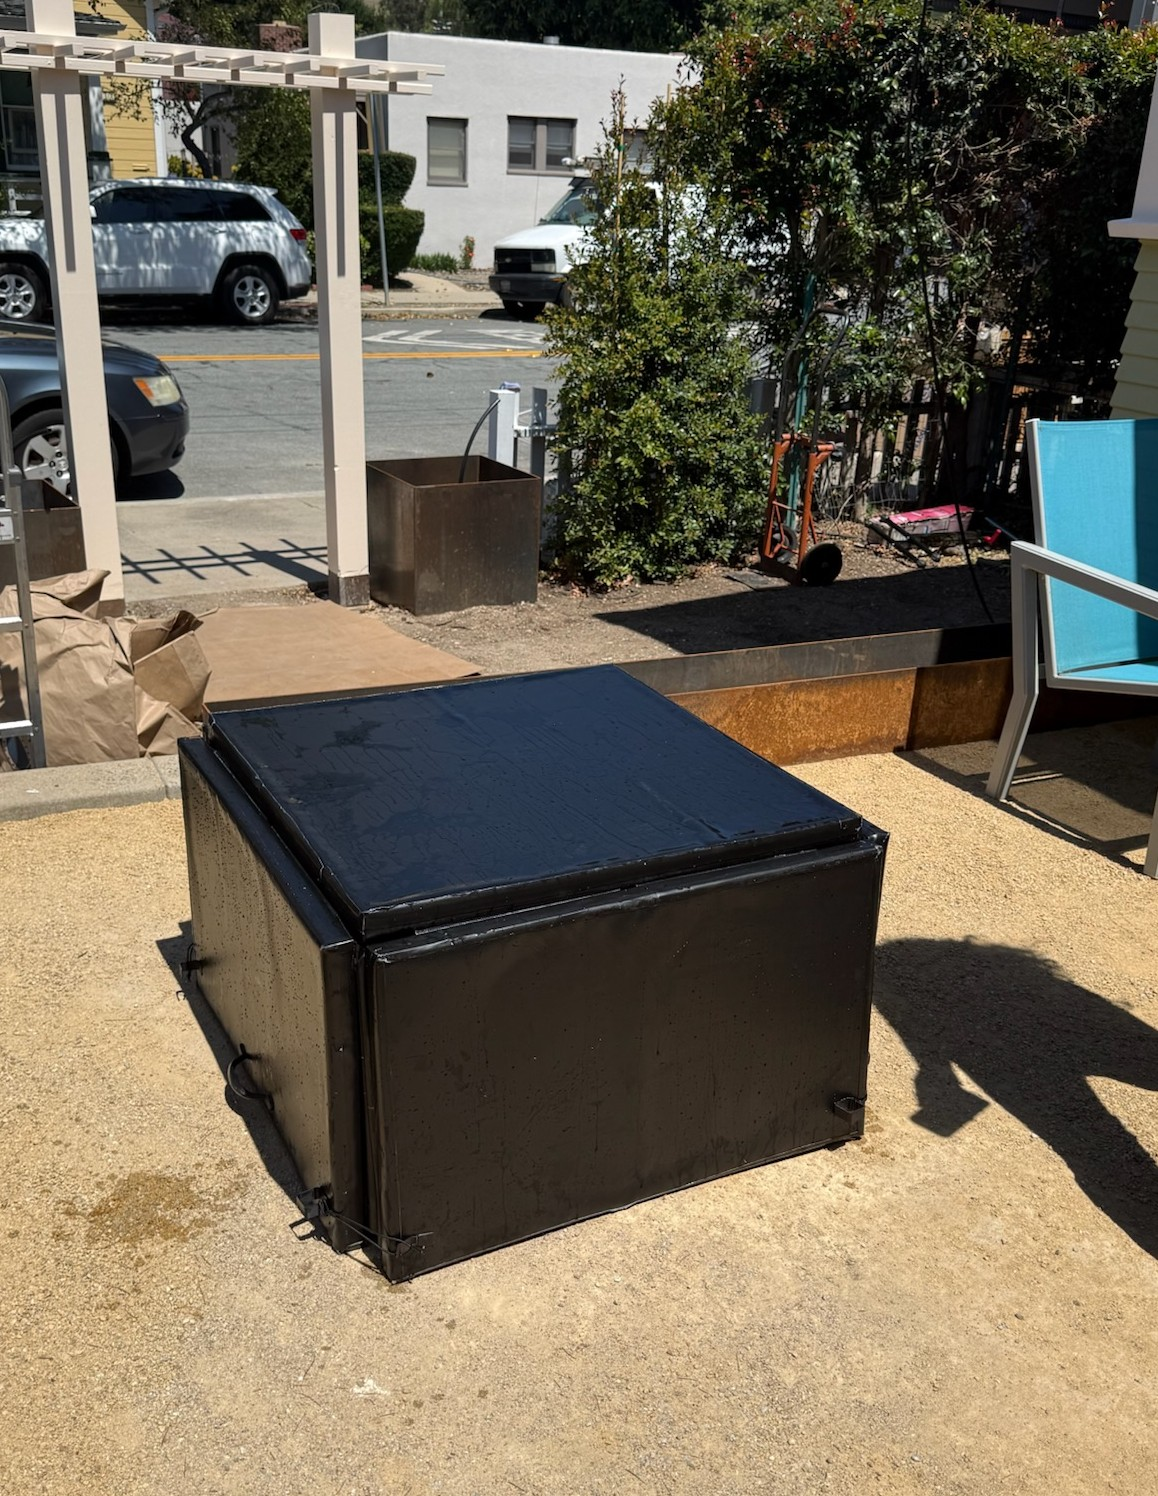
\includegraphics[
        width=1.58in,
        height=1.28in,
        keepaspectratio
    ]{foam_model_folded_backyard_image}
};
\end{scope}

\draw[RuleGray,line width=0.55pt,rounded corners=4pt]
    ($(current page.north west)+(9.19in,-5.04in)$)
    rectangle
    ($(current page.north east)+(-0.43in,-6.43in)$);

% Larger captions
\node[anchor=north,align=center,text width=1.95in,text=Muted,
      font=\sffamily\fontsize{6.8}{7.4}\selectfont]
at ($(current page.north west)+(1.47in,-6.49in)$)
{Topside panel architecture};

\node[anchor=north,align=center,text width=1.95in,text=Muted,
      font=\sffamily\fontsize{6.8}{7.4}\selectfont]
at ($(current page.north west)+(3.66in,-6.49in)$)
{Underside hinge architecture};

\node[anchor=north,align=center,text width=1.95in,text=Muted,
      font=\sffamily\fontsize{6.8}{7.4}\selectfont]
at ($(current page.north west)+(5.85in,-6.49in)$)
{Folded CAD configuration};

\node[anchor=north,align=center,text width=1.95in,text=Muted,
      font=\sffamily\fontsize{6.8}{7.4}\selectfont]
at ($(current page.north west)+(8.04in,-6.49in)$)
{Dual-use product vision};

\node[anchor=north,align=center,text width=1.95in,text=Muted,
      font=\sffamily\fontsize{6.8}{7.4}\selectfont]
at ($(current page.north west)+(9.88in,-6.49in)$)
{Folded foam prototype};

% Page 1 resource bar — centered and non-repeated resources
\fill[Panel,rounded corners=4pt]
    ($(current page.north west)+(0.43in,-7.05in)$)
    rectangle
    ($(current page.north east)+(-0.43in,-7.64in)$);
\draw[RuleGray,line width=0.5pt,rounded corners=4pt]
    ($(current page.north west)+(0.43in,-7.05in)$)
    rectangle
    ($(current page.north east)+(-0.43in,-7.64in)$);

\node[
    anchor=center,
    align=center,
    text=DeepGreen,
    font=\sffamily\bfseries\fontsize{6.9}{7.5}\selectfont
]
at ($(current page.north)+(0,-7.345in)$)
{\href{\ToroDrawingLink}{\faDraftingCompass\ DRAWING PACKAGE}
\hspace{24pt}
\href{\ToroDimensionsLink}{\faImage\ DIMENSION STUDY}
\hspace{24pt}
\href{\ToroProblemLink}{\faFileImage\ PROBLEM STATEMENT}};

% Footer
\node[
    anchor=south west,
    text=white,
    font=\sffamily\bfseries\fontsize{7.1}{7.7}\selectfont
]
at ($(current page.south west)+(0.42in,0.17in)$)
{\hyperlink{composites}{\faArrowLeft\ COMPOSITES}};

\node[
    anchor=south,
    text=white,
    font=\sffamily\fontsize{7.0}{7.6}\selectfont
]
at ($(current page.south)+(0,0.17in)$)
{TORO COVER \hspace{6pt} 1 / 3};

\node[
    anchor=south east,
    text=white,
    font=\sffamily\bfseries\fontsize{7.1}{7.7}\selectfont
]
at ($(current page.south east)+(-0.42in,0.17in)$)
{MANUFACTURING-DRIVEN DESIGN \faArrowRight};

\end{tikzpicture}


% ============================================================
% PAGE 2 — MANUFACTURING-DRIVEN DESIGN
% ============================================================

\clearpage
\thispagestyle{empty}
\hypertarget{toro-manufacturing}{}
\null

\begin{tikzpicture}[remember picture,overlay]

% Background and bars
\fill[white]
    (current page.south west)
    rectangle
    (current page.north east);

\fill[DeepGreen]
    (current page.north west)
    rectangle
    ($(current page.north east)+(0,-0.095in)$);

\fill[PolyGold]
    ($(current page.north west)+(0,-0.095in)$)
    rectangle
    ($(current page.north east)+(0,-0.14in)$);

\fill[DeepGreen]
    (current page.south west)
    rectangle
    ($(current page.south east)+(0,0.36in)$);

\fill[PolyGold]
    ($(current page.south west)+(0,0.36in)$)
    rectangle
    ($(current page.south east)+(0,0.405in)$);

% Header
\node[
    anchor=north west,
    text=PolyGold,
    font=\sffamily\bfseries\fontsize{8.1}{8.7}\selectfont
]
at ($(current page.north west)+(0.42in,-0.39in)$)
{TORO COVER \hspace{5pt}/\hspace{5pt} DESIGN FOR MANUFACTURABILITY};

\node[
    anchor=north west,
    text=DeepGreen,
    font=\bfseries\fontsize{23}{24}\selectfont
]
at ($(current page.north west)+(0.40in,-0.67in)$)
{THE ENVELOPE METHOD};

\node[
    anchor=north west,
    text=Muted,
    font=\sffamily\fontsize{8.7}{9.6}\selectfont
]
at ($(current page.north west)+(0.42in,-1.12in)$)
{A one-layup process developed for unusually thick insulated composite sandwich panels};

\fill[PolyGold]
    ($(current page.north west)+(0.42in,-1.36in)$)
    rectangle
    ($(current page.north west)+(5.30in,-1.315in)$);

% Process explanation
\fill[SoftGold,rounded corners=5pt]
    ($(current page.north west)+(0.42in,-1.61in)$)
    rectangle
    ($(current page.north east)+(-0.42in,-2.90in)$);

\fill[PolyGold]
    ($(current page.north west)+(0.42in,-1.61in)$)
    rectangle
    ($(current page.north west)+(0.52in,-2.90in)$);

\node[
    anchor=north west,
    text=DeepGreen,
    font=\sffamily\bfseries\fontsize{7.9}{8.6}\selectfont
]
at ($(current page.north west)+(0.67in,-1.76in)$)
{PROCESS INNOVATION};

\node[
    anchor=north west,
    align=left,
    text width=9.55in,
    text=Ink,
    font=\fontsize{7.35}{8.75}\selectfont
]
at ($(current page.north west)+(0.67in,-2.02in)$)
{
Weight reduction and insulation were both essential, leading to the selection of an
XPS foam core. Because XPS could not tolerate composite heat-cure temperatures, prepreg
processing was not practical and the panels had to be manufactured by wet layup with a
room-temperature cure. To simplify this process, I waterjet-cut XPS perimeter strips from
excess foam and placed them around each core inside the vacuum enclosure. Under vacuum,
the top and bottom carbon skins met along the panel sides and compressed against this
border, eliminating a separate edge-banding layup and reducing corner pleating.
};

% Workflow title
\node[
    anchor=north west,
    text=DeepGreen,
    font=\sffamily\bfseries\fontsize{8.0}{8.7}\selectfont
]
at ($(current page.north west)+(0.43in,-3.06in)$)
{MANUFACTURING WORKFLOW};

% Row 1 image 1
\node[anchor=center,inner sep=0pt]
at ($(current page.north west)+(2.07in,-4.105in)$)
{
    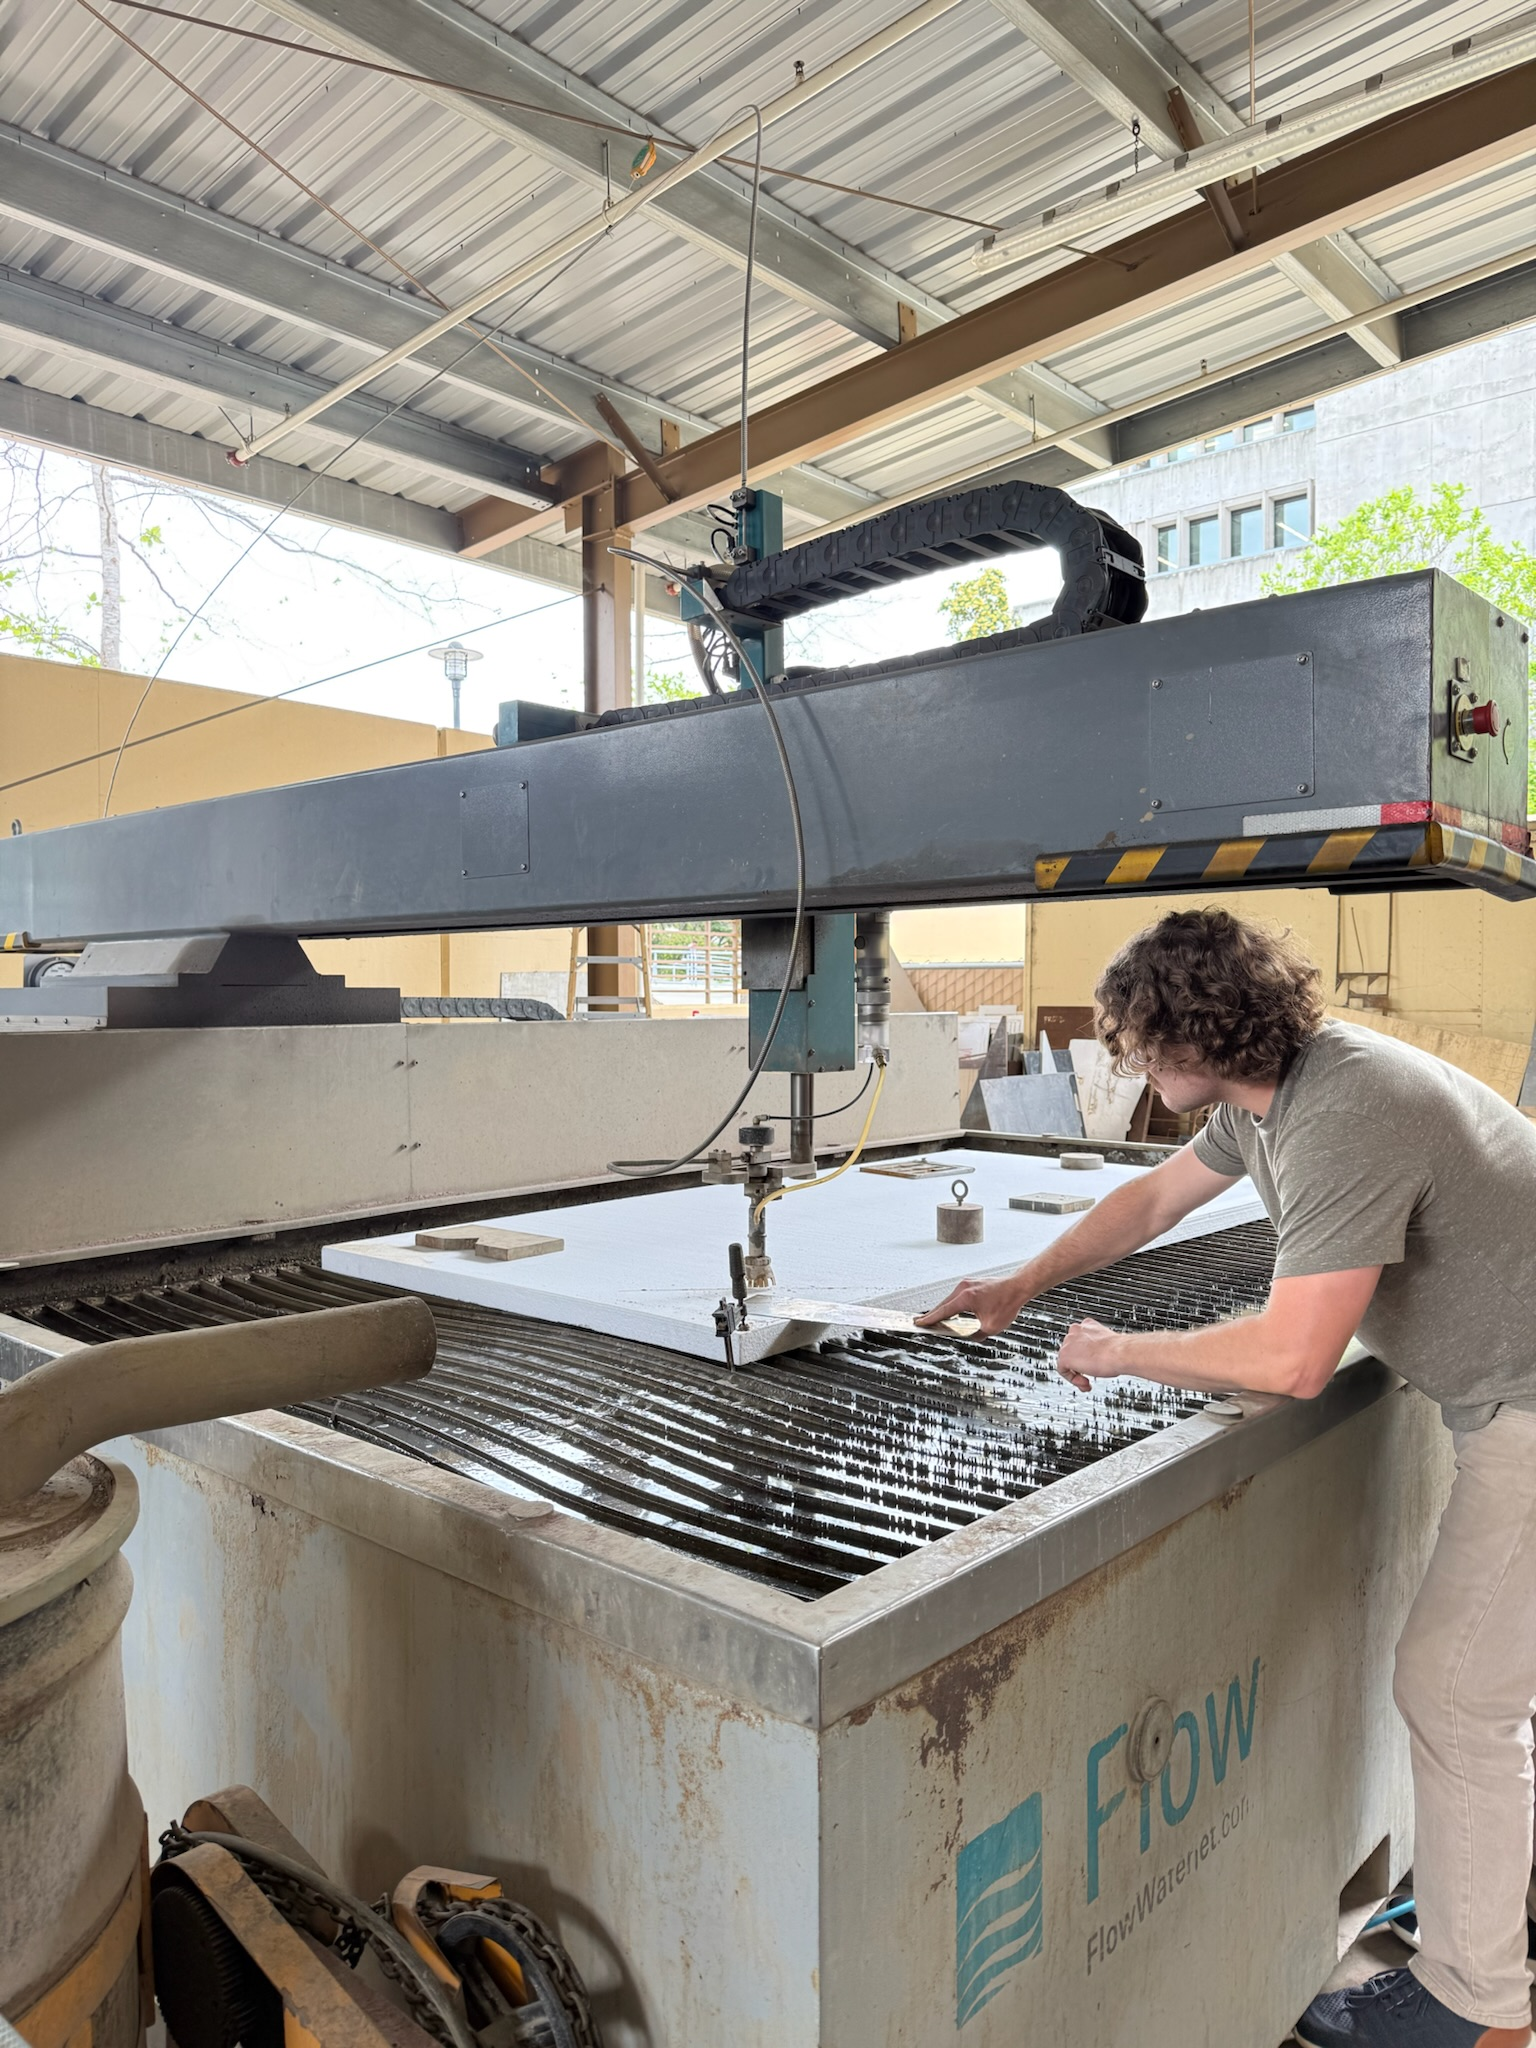
\includegraphics[
        width=3.10in,
        height=1.40in,
        keepaspectratio
    ]{waterjet_foam}
};
\draw[RuleGray,line width=0.55pt,rounded corners=4pt]
    ($(current page.north west)+(0.43in,-3.36in)$)
    rectangle
    ($(current page.north west)+(3.71in,-4.85in)$);

% Row 1 image 2
\node[anchor=center,inner sep=0pt]
at ($(current page.north west)+(5.50in,-4.105in)$)
{
    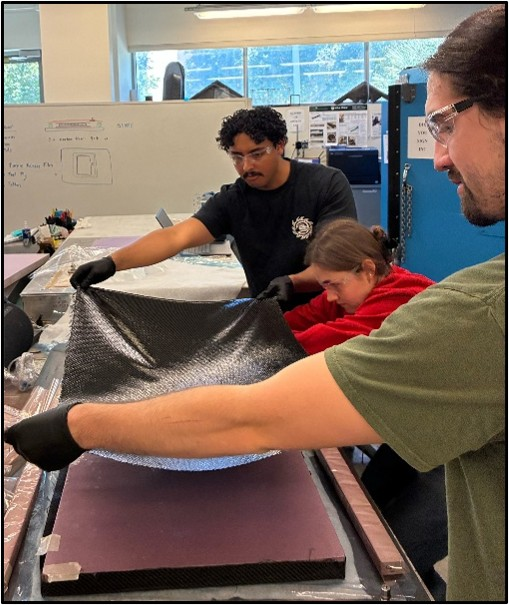
\includegraphics[
        width=3.10in,
        height=1.40in,
        keepaspectratio
    ]{group_layup}
};
\draw[RuleGray,line width=0.55pt,rounded corners=4pt]
    ($(current page.north west)+(3.86in,-3.36in)$)
    rectangle
    ($(current page.north west)+(7.14in,-4.85in)$);

% Row 1 image 3
\node[anchor=center,inner sep=0pt]
at ($(current page.north west)+(8.935in,-4.105in)$)
{
    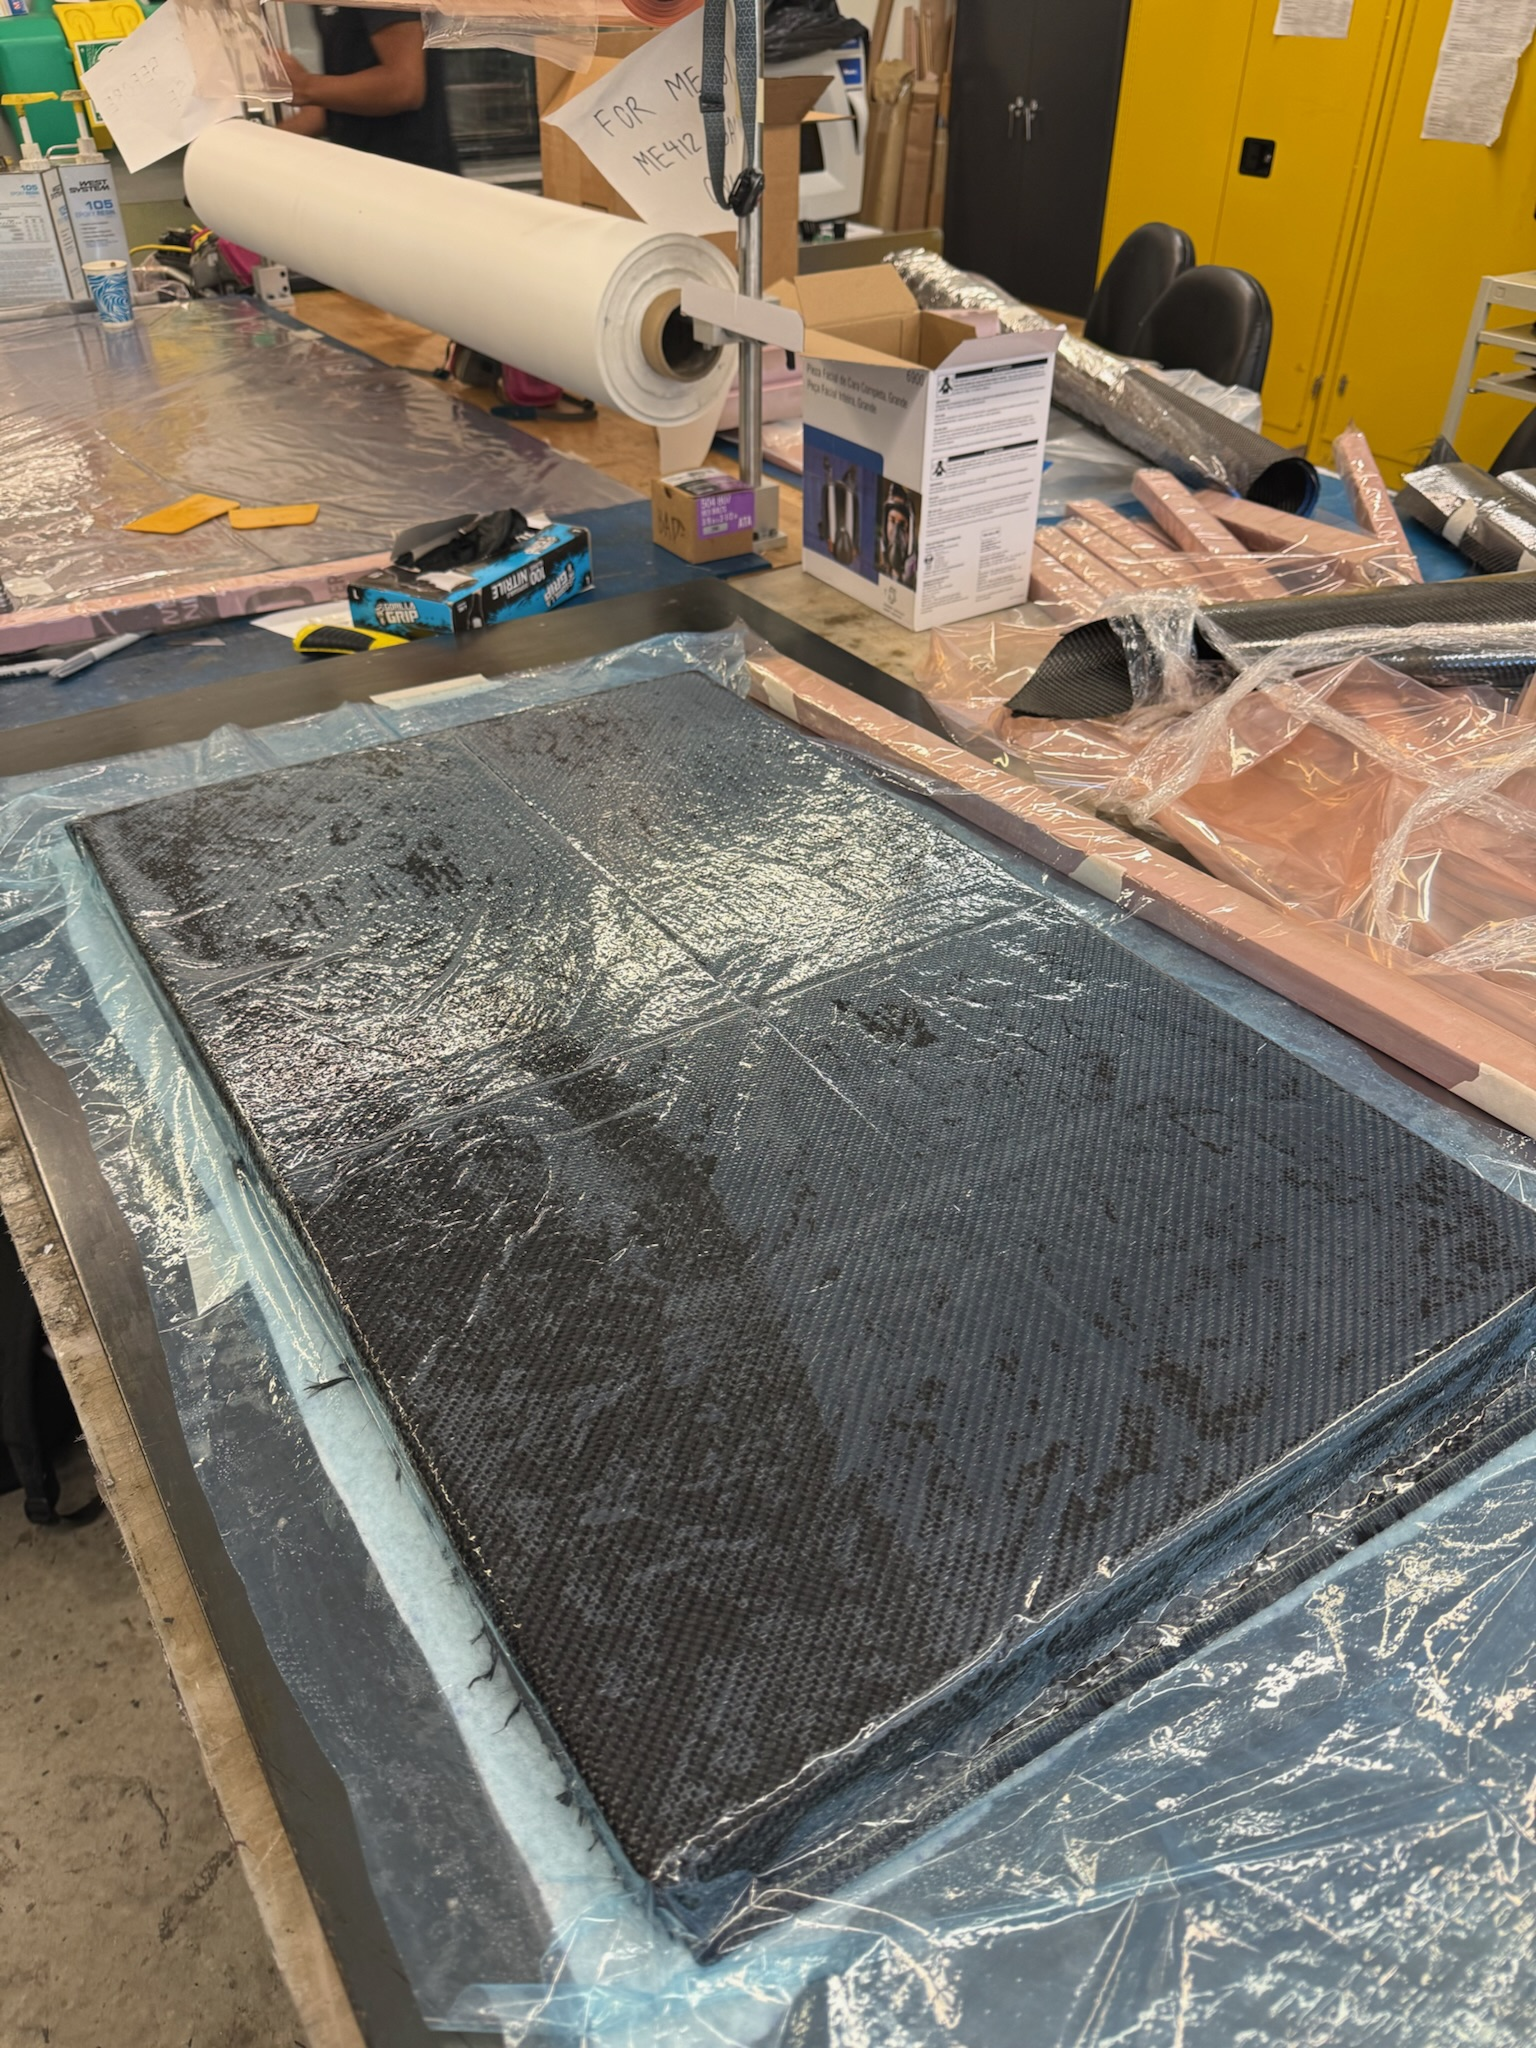
\includegraphics[
        width=3.10in,
        height=1.40in,
        keepaspectratio
    ]{blue_perforrated_film_layup}
};
\draw[RuleGray,line width=0.55pt,rounded corners=4pt]
    ($(current page.north west)+(7.29in,-3.36in)$)
    rectangle
    ($(current page.north east)+(-0.42in,-4.85in)$);

% Row 1 captions
\node[anchor=north,text=Muted,font=\sffamily\fontsize{6.7}{7.3}\selectfont]
at ($(current page.north west)+(2.07in,-4.90in)$)
{1. Waterjet-cut core and perimeter geometry};

\node[anchor=north,text=Muted,font=\sffamily\fontsize{6.7}{7.3}\selectfont]
at ($(current page.north west)+(5.50in,-4.90in)$)
{2. Team wet layup under my process guidance};

\node[anchor=north,text=Muted,font=\sffamily\fontsize{6.7}{7.3}\selectfont]
at ($(current page.north west)+(8.935in,-4.90in)$)
{3. Perforated film, breather, and vacuum enclosure};

% Row 2 image 1
\node[anchor=center,inner sep=0pt]
at ($(current page.north west)+(2.07in,-5.875in)$)
{
    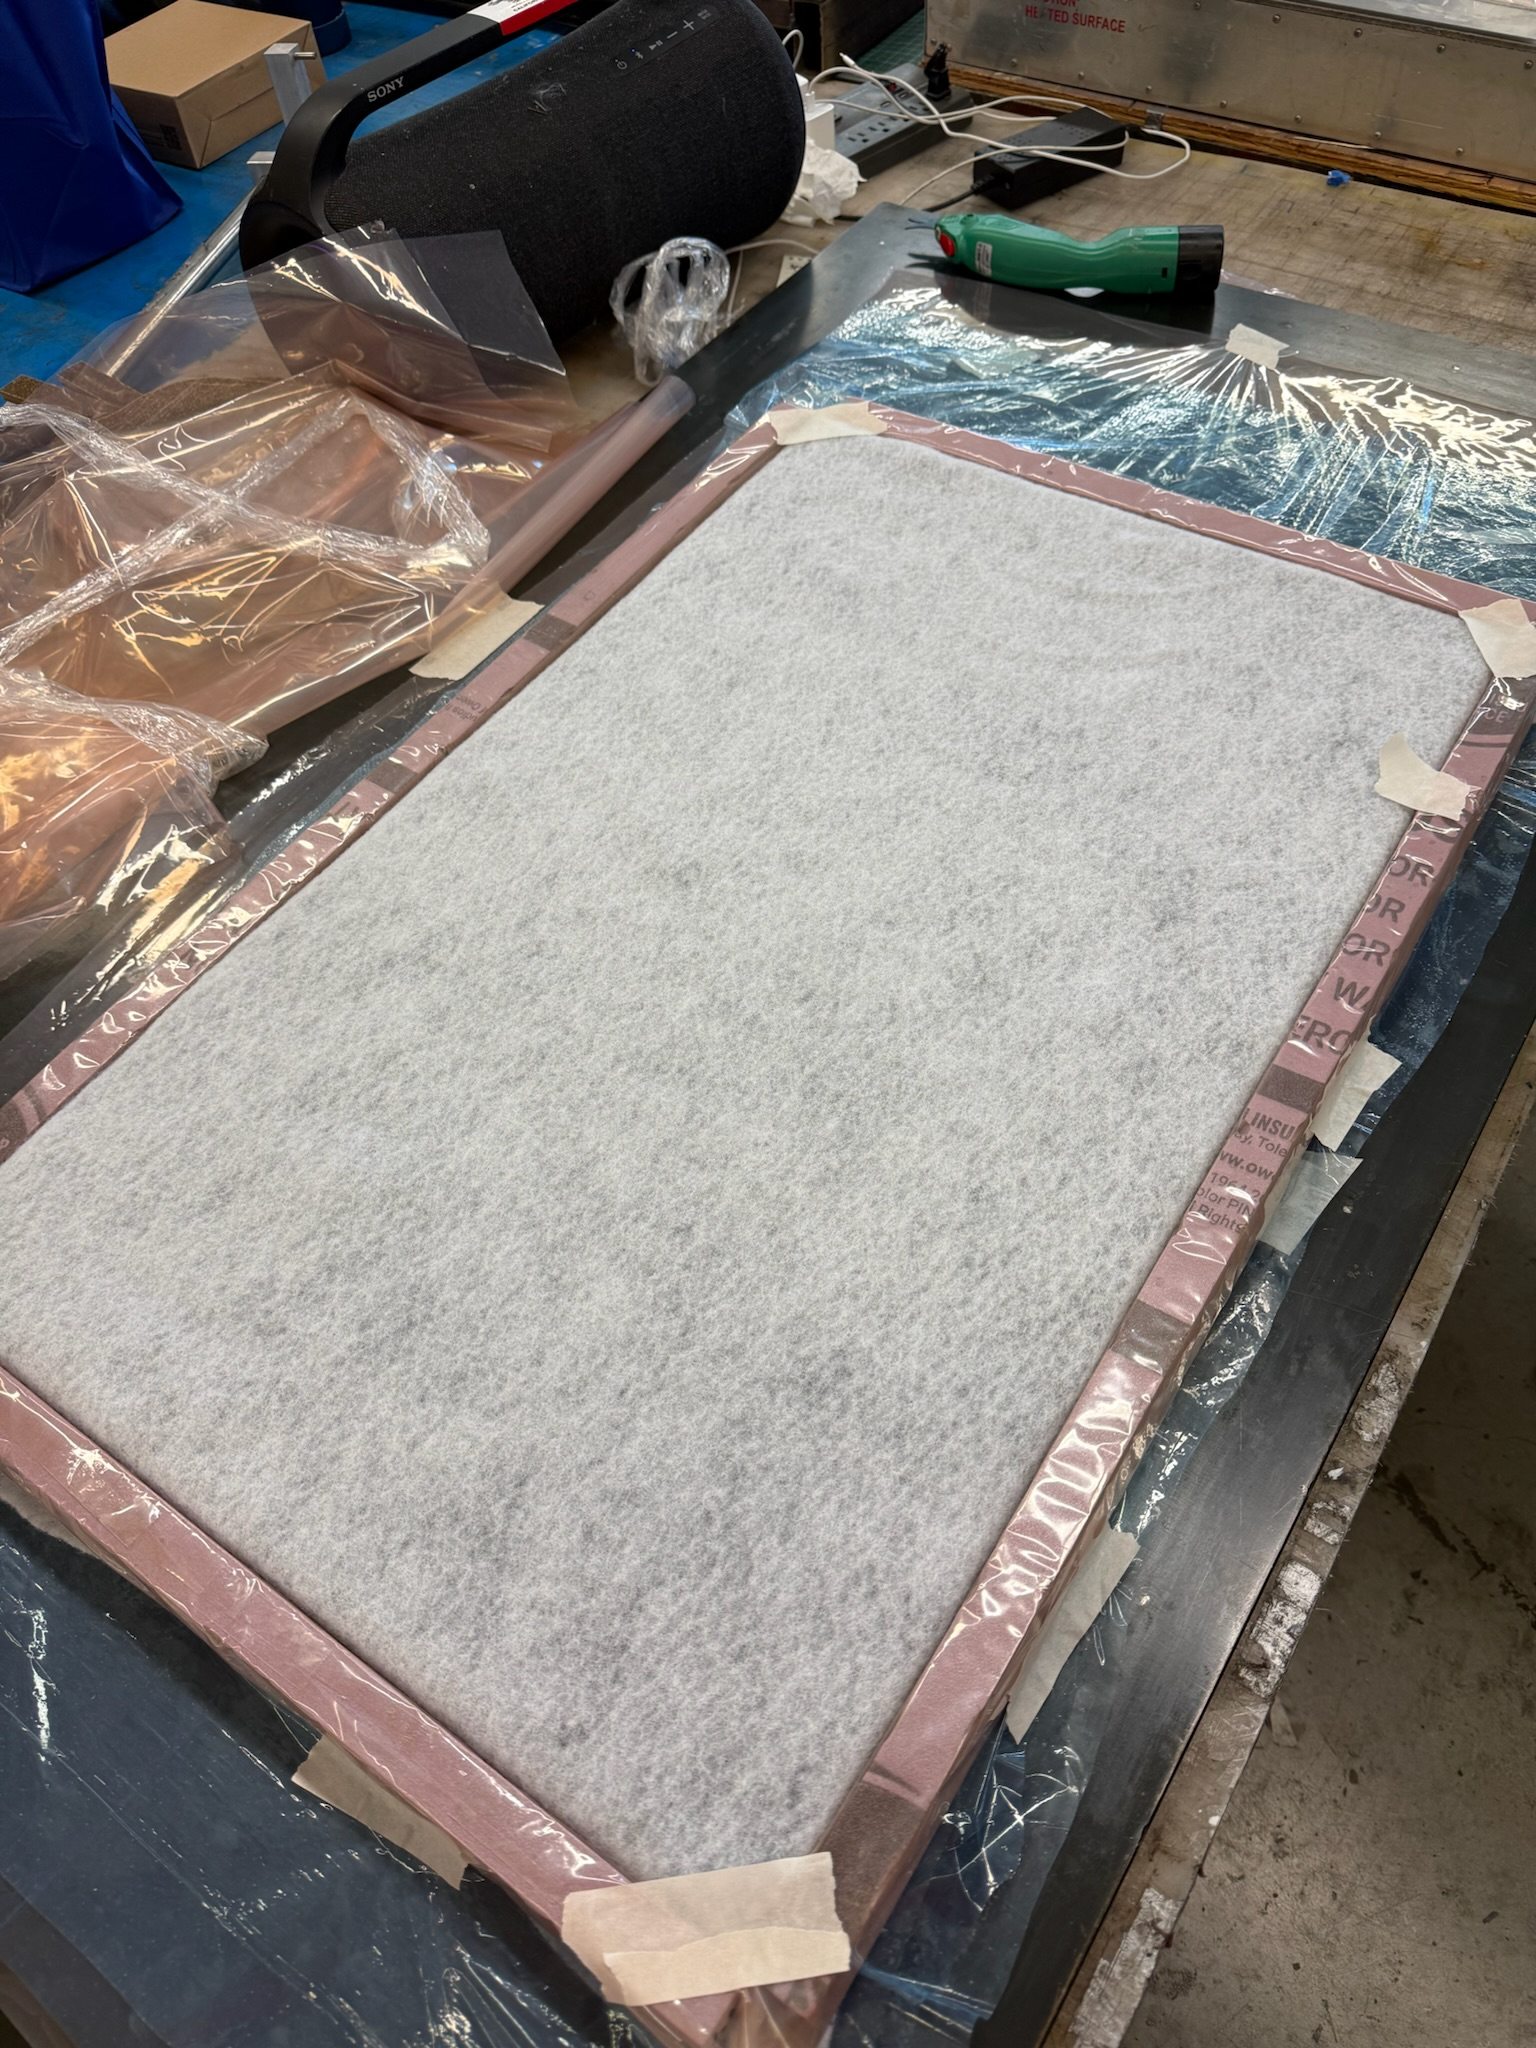
\includegraphics[
        width=3.10in,
        height=1.40in,
        keepaspectratio
    ]{completed_layup}
};
\draw[RuleGray,line width=0.55pt,rounded corners=4pt]
    ($(current page.north west)+(0.43in,-5.13in)$)
    rectangle
    ($(current page.north west)+(3.71in,-6.62in)$);

% Row 2 image 2 — oven chamber used only as a reliable vacuum enclosure; no heat applied
\node[anchor=center,inner sep=0pt]
at ($(current page.north west)+(5.50in,-5.875in)$)
{
    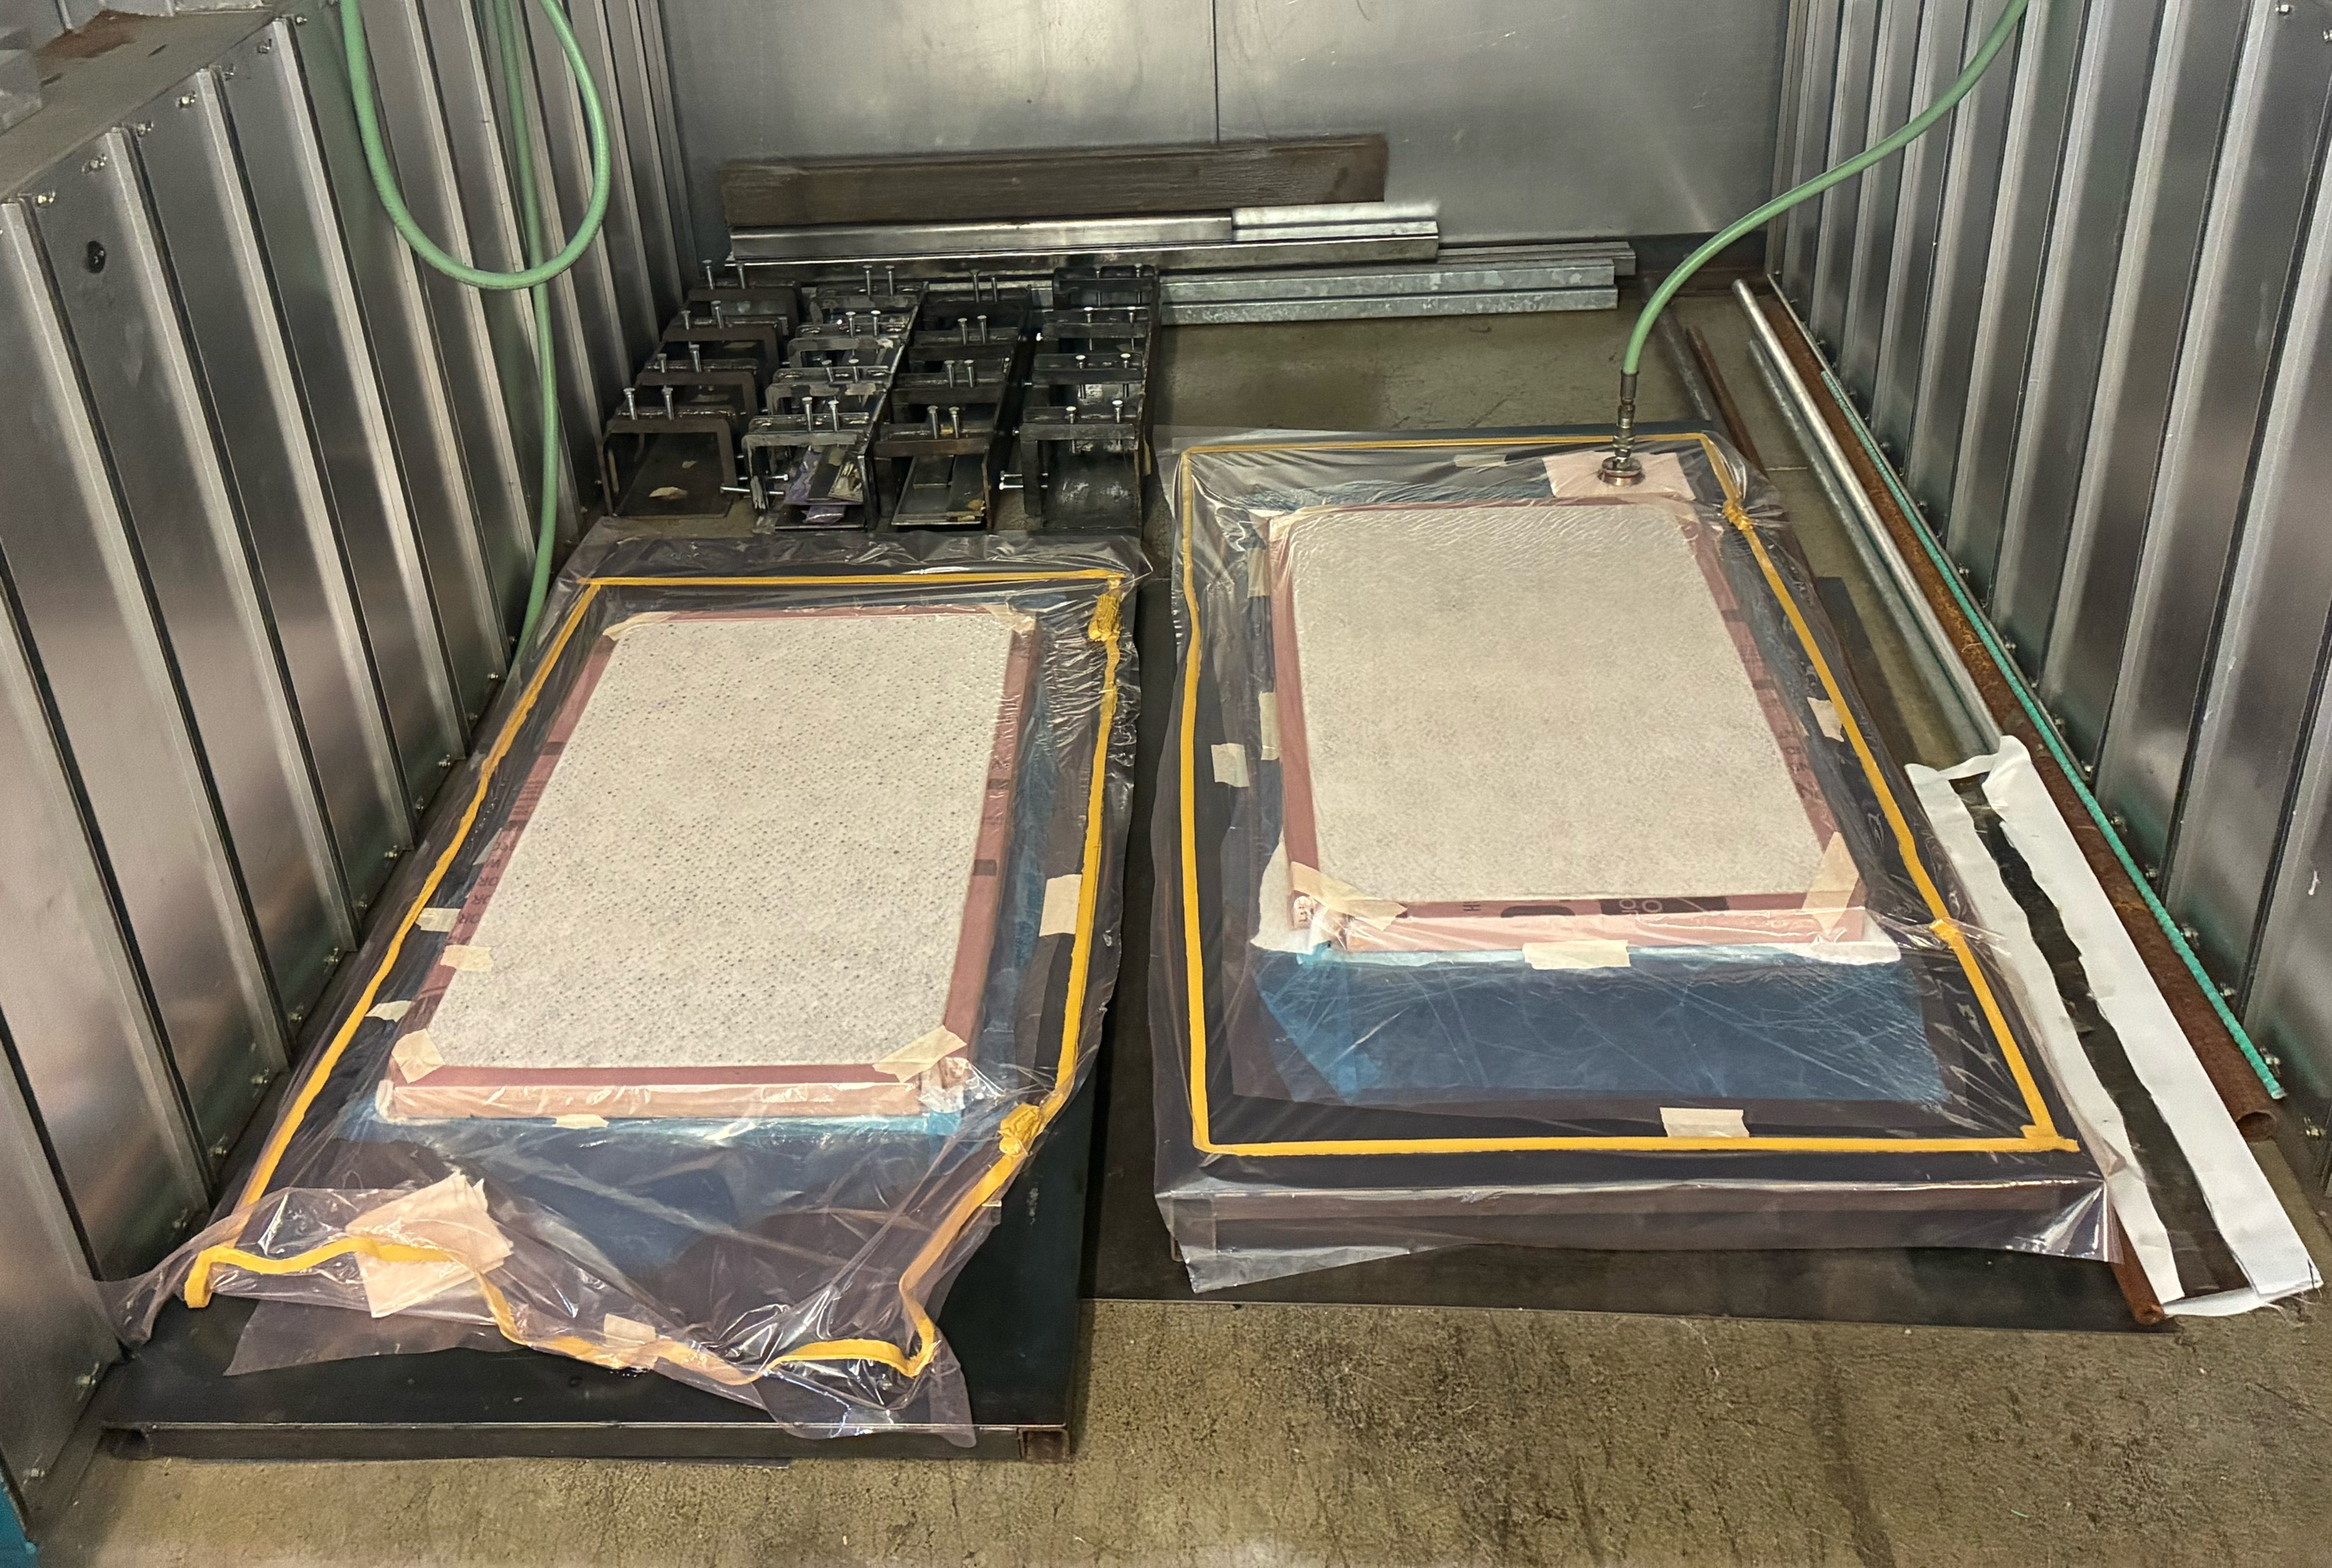
\includegraphics[
        width=3.10in,
        height=1.40in,
        keepaspectratio
    ]{layups_in_composite_oven_under_vacuumPressure}
};
\draw[RuleGray,line width=0.55pt,rounded corners=4pt]
    ($(current page.north west)+(3.86in,-5.13in)$)
    rectangle
    ($(current page.north west)+(7.14in,-6.62in)$);

% Row 2 image 3
\node[anchor=center,inner sep=0pt]
at ($(current page.north west)+(8.935in,-5.875in)$)
{
    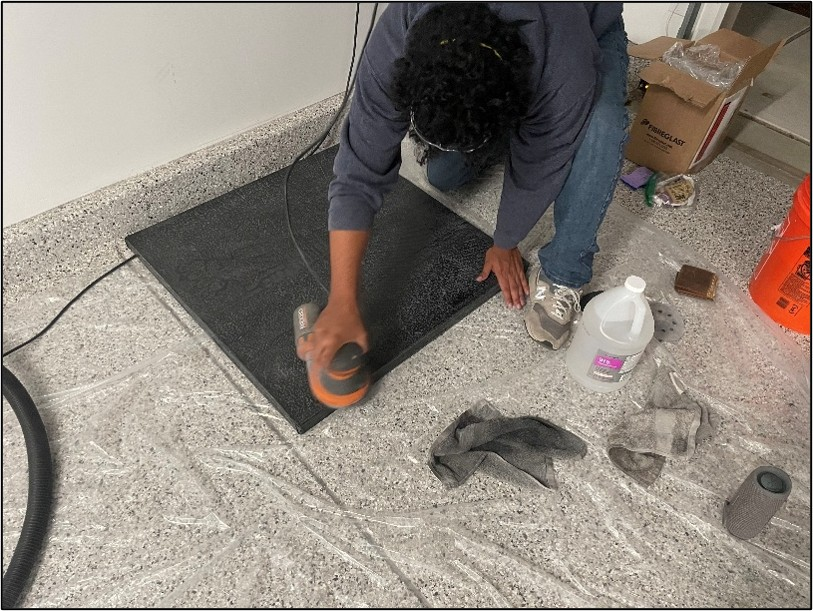
\includegraphics[
        width=3.10in,
        height=1.40in,
        keepaspectratio
    ]{garage_sanding}
};
\draw[RuleGray,line width=0.55pt,rounded corners=4pt]
    ($(current page.north west)+(7.29in,-5.13in)$)
    rectangle
    ($(current page.north east)+(-0.42in,-6.62in)$);

% Row 2 captions
\node[anchor=north,text=Muted,font=\sffamily\fontsize{6.7}{7.3}\selectfont]
at ($(current page.north west)+(2.07in,-6.67in)$)
{4. Fully saturated carbon skin and foam sandwich};

\node[anchor=north,text=Muted,font=\sffamily\fontsize{6.7}{7.3}\selectfont]
at ($(current page.north west)+(5.50in,-6.67in)$)
{5. Room-temperature cure under continuous vacuum};

\node[anchor=north,text=Muted,font=\sffamily\fontsize{6.7}{7.3}\selectfont]
at ($(current page.north west)+(8.935in,-6.67in)$)
{6. Post-processing and surface preparation};

% Bottom callouts
\fill[Panel,rounded corners=4pt]
    ($(current page.north west)+(0.43in,-6.95in)$)
    rectangle
    ($(current page.north west)+(5.48in,-7.60in)$);

\draw[RuleGray,line width=0.55pt,rounded corners=4pt]
    ($(current page.north west)+(0.43in,-6.95in)$)
    rectangle
    ($(current page.north west)+(5.48in,-7.60in)$);

\node[
    anchor=north west,
    text=DeepGreen,
    font=\sffamily\bfseries\fontsize{7.0}{7.6}\selectfont
]
at ($(current page.north west)+(0.63in,-7.08in)$)
{FROM THREE LAYUPS TO ONE};

\node[
    anchor=north west,
    align=left,
    text width=4.56in,
    text=Ink,
    font=\fontsize{6.45}{7.45}\selectfont
]
at ($(current page.north west)+(0.63in,-7.29in)$)
{
The Envelope Method reduced labor, cure cycles, handling,
alignment risk, and time spent forming numerous vacuum-bag
pleats around the 1.5-inch-thick XPS panels.
};

\fill[Panel,rounded corners=4pt]
    ($(current page.north west)+(5.68in,-6.95in)$)
    rectangle
    ($(current page.north east)+(-0.42in,-7.60in)$);

\draw[RuleGray,line width=0.55pt,rounded corners=4pt]
    ($(current page.north west)+(5.68in,-6.95in)$)
    rectangle
    ($(current page.north east)+(-0.42in,-7.60in)$);

\node[
    anchor=north west,
    text=DeepGreen,
    font=\sffamily\bfseries\fontsize{7.0}{7.6}\selectfont
]
at ($(current page.north west)+(5.88in,-7.08in)$)
{WHY SURFACE-BONDED HARDWARE};

\node[
    anchor=north west,
    align=left,
    text width=4.55in,
    text=Ink,
    font=\fontsize{6.45}{7.45}\selectfont
]
at ($(current page.north west)+(5.88in,-7.29in)$)
{
Adhesively bonded hinges and fixtures preserved the clean
composite exterior and avoided drilled inserts, foam-core
crushing, added stress concentrations, and new leak paths.
};


% Footer
\node[
    anchor=south west,
    text=white,
    font=\sffamily\bfseries\fontsize{7.1}{7.7}\selectfont
]
at ($(current page.south west)+(0.42in,0.17in)$)
{\faArrowLeft\ PRODUCT ARCHITECTURE};

\node[
    anchor=south,
    text=white,
    font=\sffamily\fontsize{7.0}{7.6}\selectfont
]
at ($(current page.south)+(0,0.17in)$)
{TORO COVER \hspace{6pt} 2 / 3};

\node[
    anchor=south east,
    text=white,
    font=\sffamily\bfseries\fontsize{7.1}{7.7}\selectfont
]
at ($(current page.south east)+(-0.42in,0.17in)$)
{VALIDATION \& TAKEAWAYS \faArrowRight};

\end{tikzpicture}


% ============================================================
% PAGE 3 — FINISHING, VALIDATION, AND TAKEAWAYS
% ============================================================

\clearpage
\thispagestyle{empty}
\hypertarget{toro-results}{}
\null

\begin{tikzpicture}[remember picture,overlay]

% Background and bars
\fill[white]
    (current page.south west)
    rectangle
    (current page.north east);

\fill[DeepGreen]
    (current page.north west)
    rectangle
    ($(current page.north east)+(0,-0.095in)$);

\fill[PolyGold]
    ($(current page.north west)+(0,-0.095in)$)
    rectangle
    ($(current page.north east)+(0,-0.14in)$);

\fill[DeepGreen]
    (current page.south west)
    rectangle
    ($(current page.south east)+(0,0.36in)$);

\fill[PolyGold]
    ($(current page.south west)+(0,0.36in)$)
    rectangle
    ($(current page.south east)+(0,0.405in)$);

% Header
\node[
    anchor=north west,
    text=PolyGold,
    font=\sffamily\bfseries\fontsize{8.1}{8.7}\selectfont
]
at ($(current page.north west)+(0.42in,-0.39in)$)
{TORO COVER \hspace{5pt}/\hspace{5pt} VALIDATION AND ENGINEERING TAKEAWAYS};

\node[
    anchor=north west,
    text=DeepGreen,
    font=\bfseries\fontsize{22.5}{23.5}\selectfont
]
at ($(current page.north west)+(0.40in,-0.67in)$)
{FROM PROTOTYPE TO PRODUCT PATHWAY};

\node[
    anchor=north west,
    text=Muted,
    font=\sffamily\fontsize{8.7}{9.6}\selectfont
]
at ($(current page.north west)+(0.42in,-1.12in)$)
{Environmental protection, usability testing, scope decisions, and lessons from technical leadership};

\fill[PolyGold]
    ($(current page.north west)+(0.42in,-1.36in)$)
    rectangle
    ($(current page.north west)+(5.8in,-1.315in)$);

% Finishing title
\node[
    anchor=north west,
    text=DeepGreen,
    font=\sffamily\bfseries\fontsize{8.0}{8.7}\selectfont
]
at ($(current page.north west)+(0.43in,-1.62in)$)
{OUTDOOR FINISHING AND ENVIRONMENTAL PROTECTION};

% Image 1
\node[anchor=center,inner sep=0pt]
at ($(current page.north west)+(1.705in,-2.655in)$)
{
    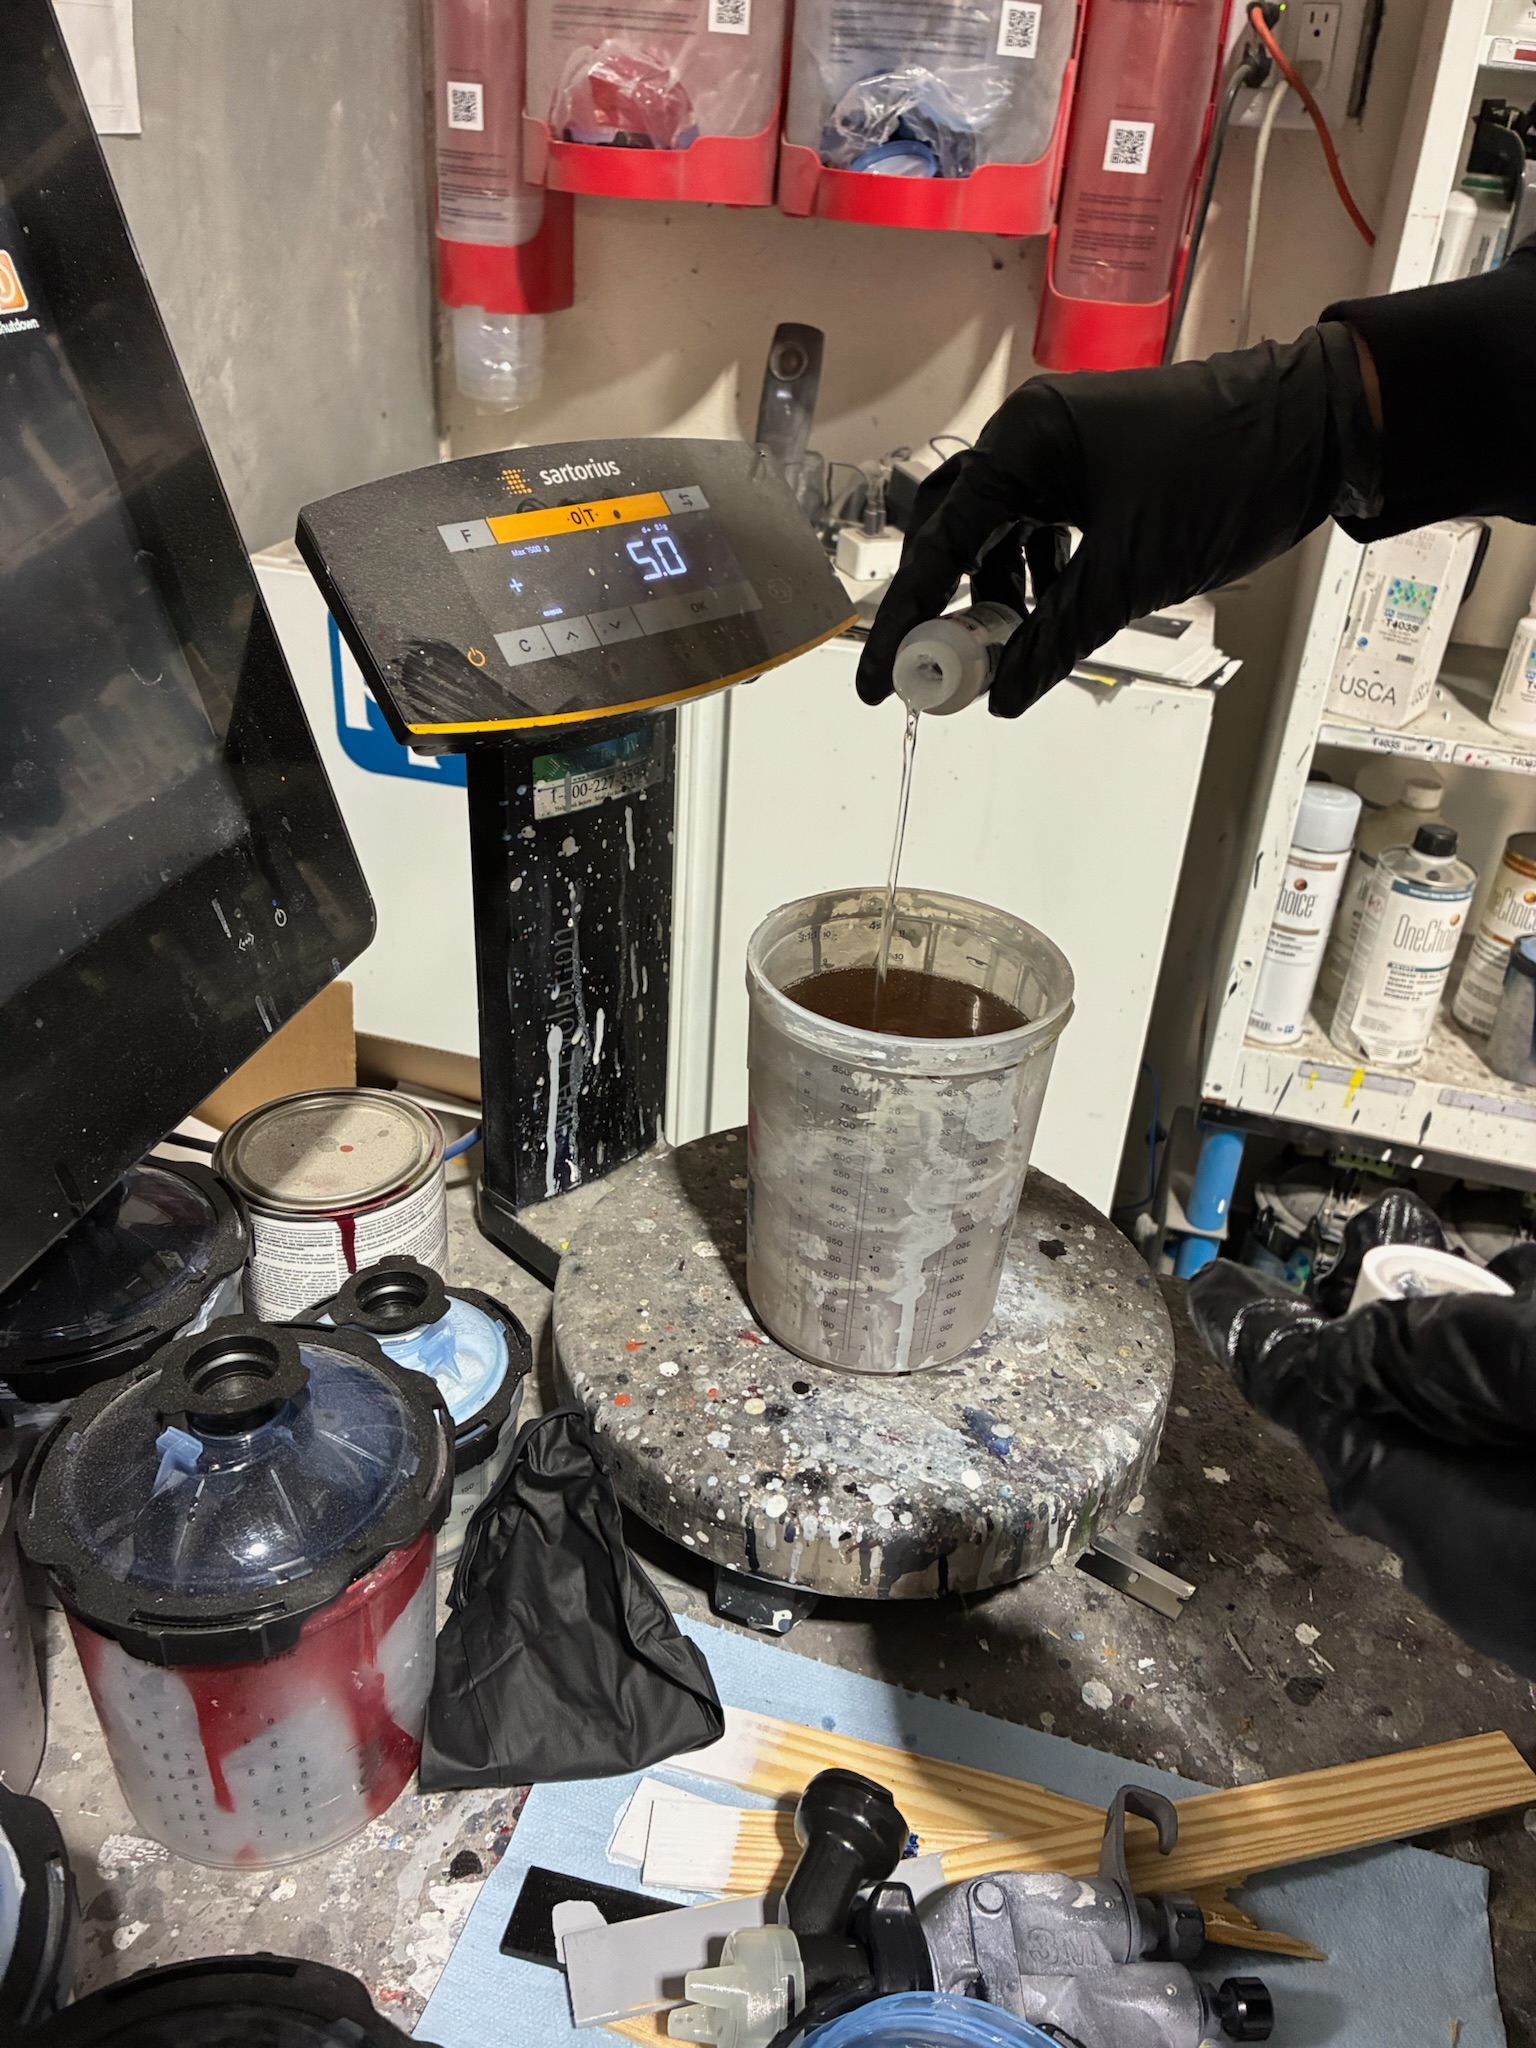
\includegraphics[
        width=2.35in,
        height=1.40in,
        keepaspectratio
    ]{spray_topcoat_prep}
};
\draw[RuleGray,line width=0.55pt,rounded corners=4pt]
    ($(current page.north west)+(0.43in,-1.91in)$)
    rectangle
    ($(current page.north west)+(2.98in,-3.40in)$);

% Image 2
\node[anchor=center,inner sep=0pt]
at ($(current page.north west)+(4.375in,-2.655in)$)
{
    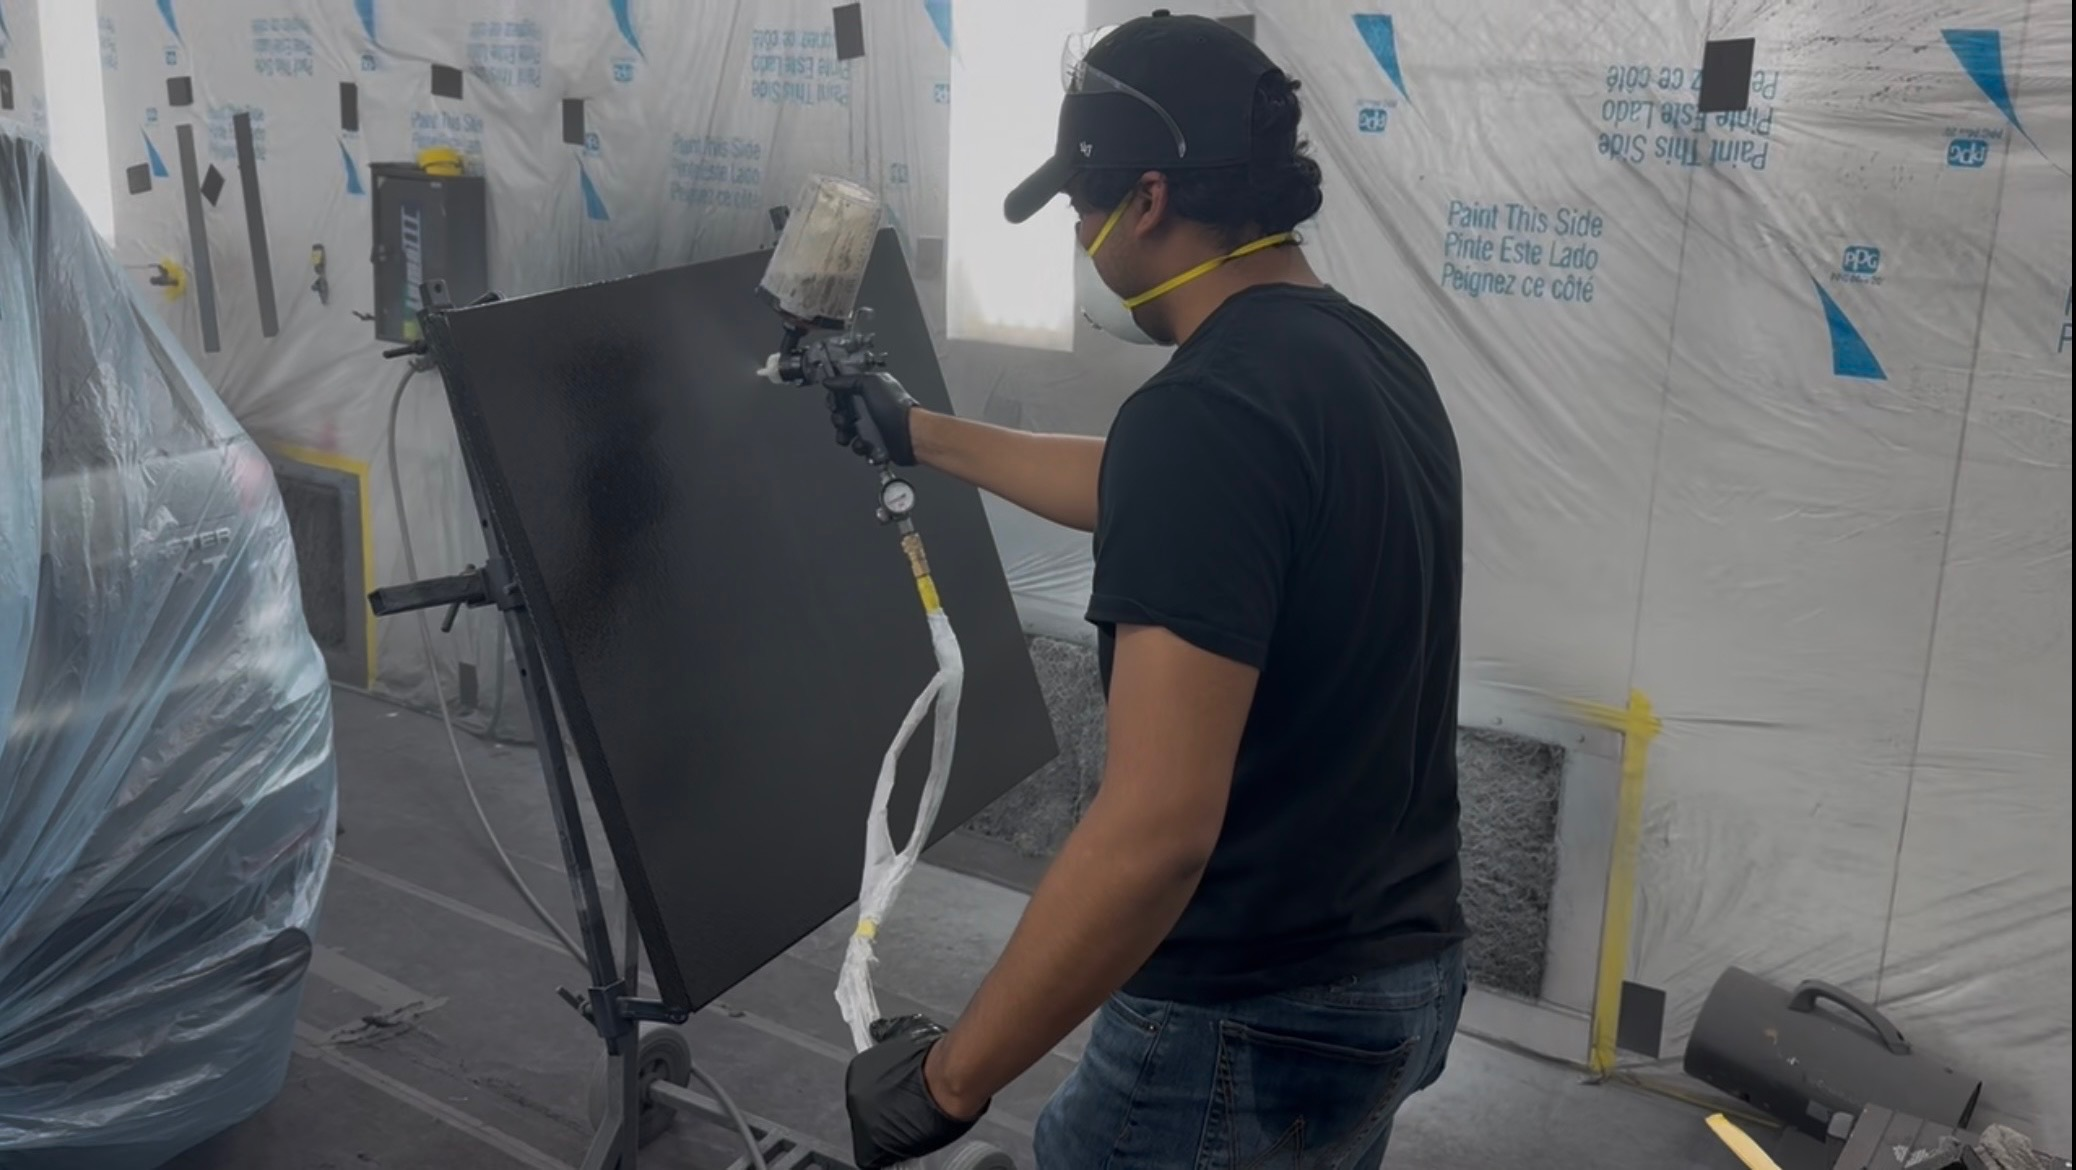
\includegraphics[
        width=2.35in,
        height=1.40in,
        keepaspectratio
    ]{spraying_topcoat}
};
\draw[RuleGray,line width=0.55pt,rounded corners=4pt]
    ($(current page.north west)+(3.10in,-1.91in)$)
    rectangle
    ($(current page.north west)+(5.65in,-3.40in)$);

% Image 3
\node[anchor=center,inner sep=0pt]
at ($(current page.north west)+(7.045in,-2.655in)$)
{
    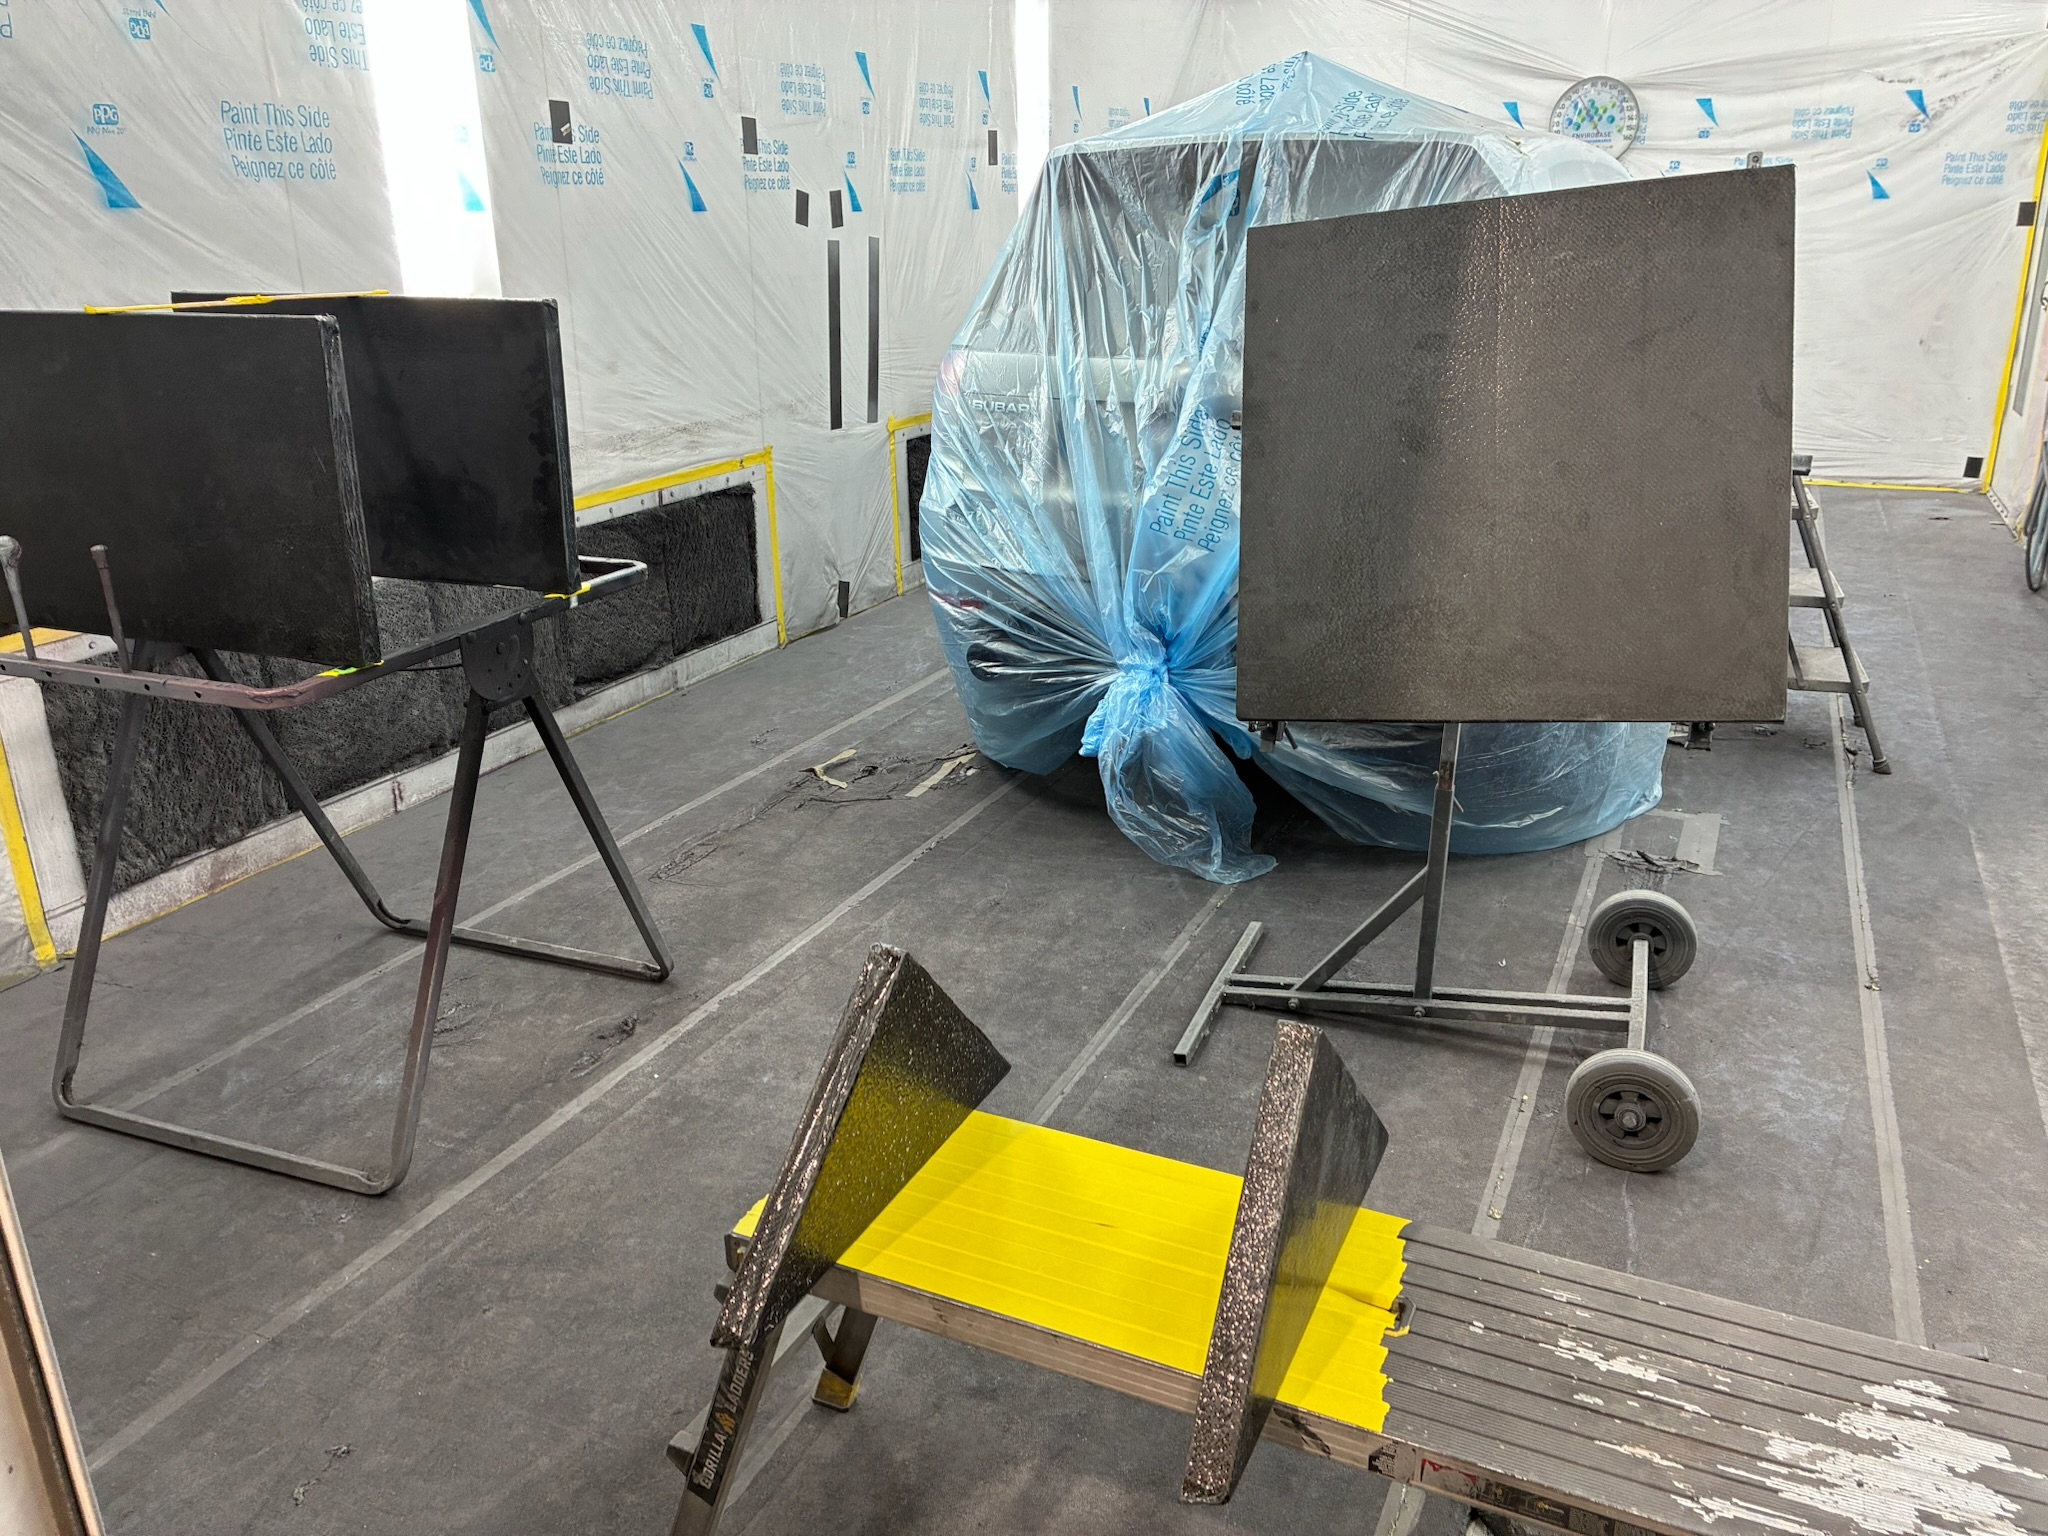
\includegraphics[
        width=2.35in,
        height=1.40in,
        keepaspectratio
    ]{topcoat_setup_apparatus}
};
\draw[RuleGray,line width=0.55pt,rounded corners=4pt]
    ($(current page.north west)+(5.77in,-1.91in)$)
    rectangle
    ($(current page.north west)+(8.32in,-3.40in)$);

% Image 4
\node[anchor=center,inner sep=0pt]
at ($(current page.north west)+(9.50in,-2.655in)$)
{
    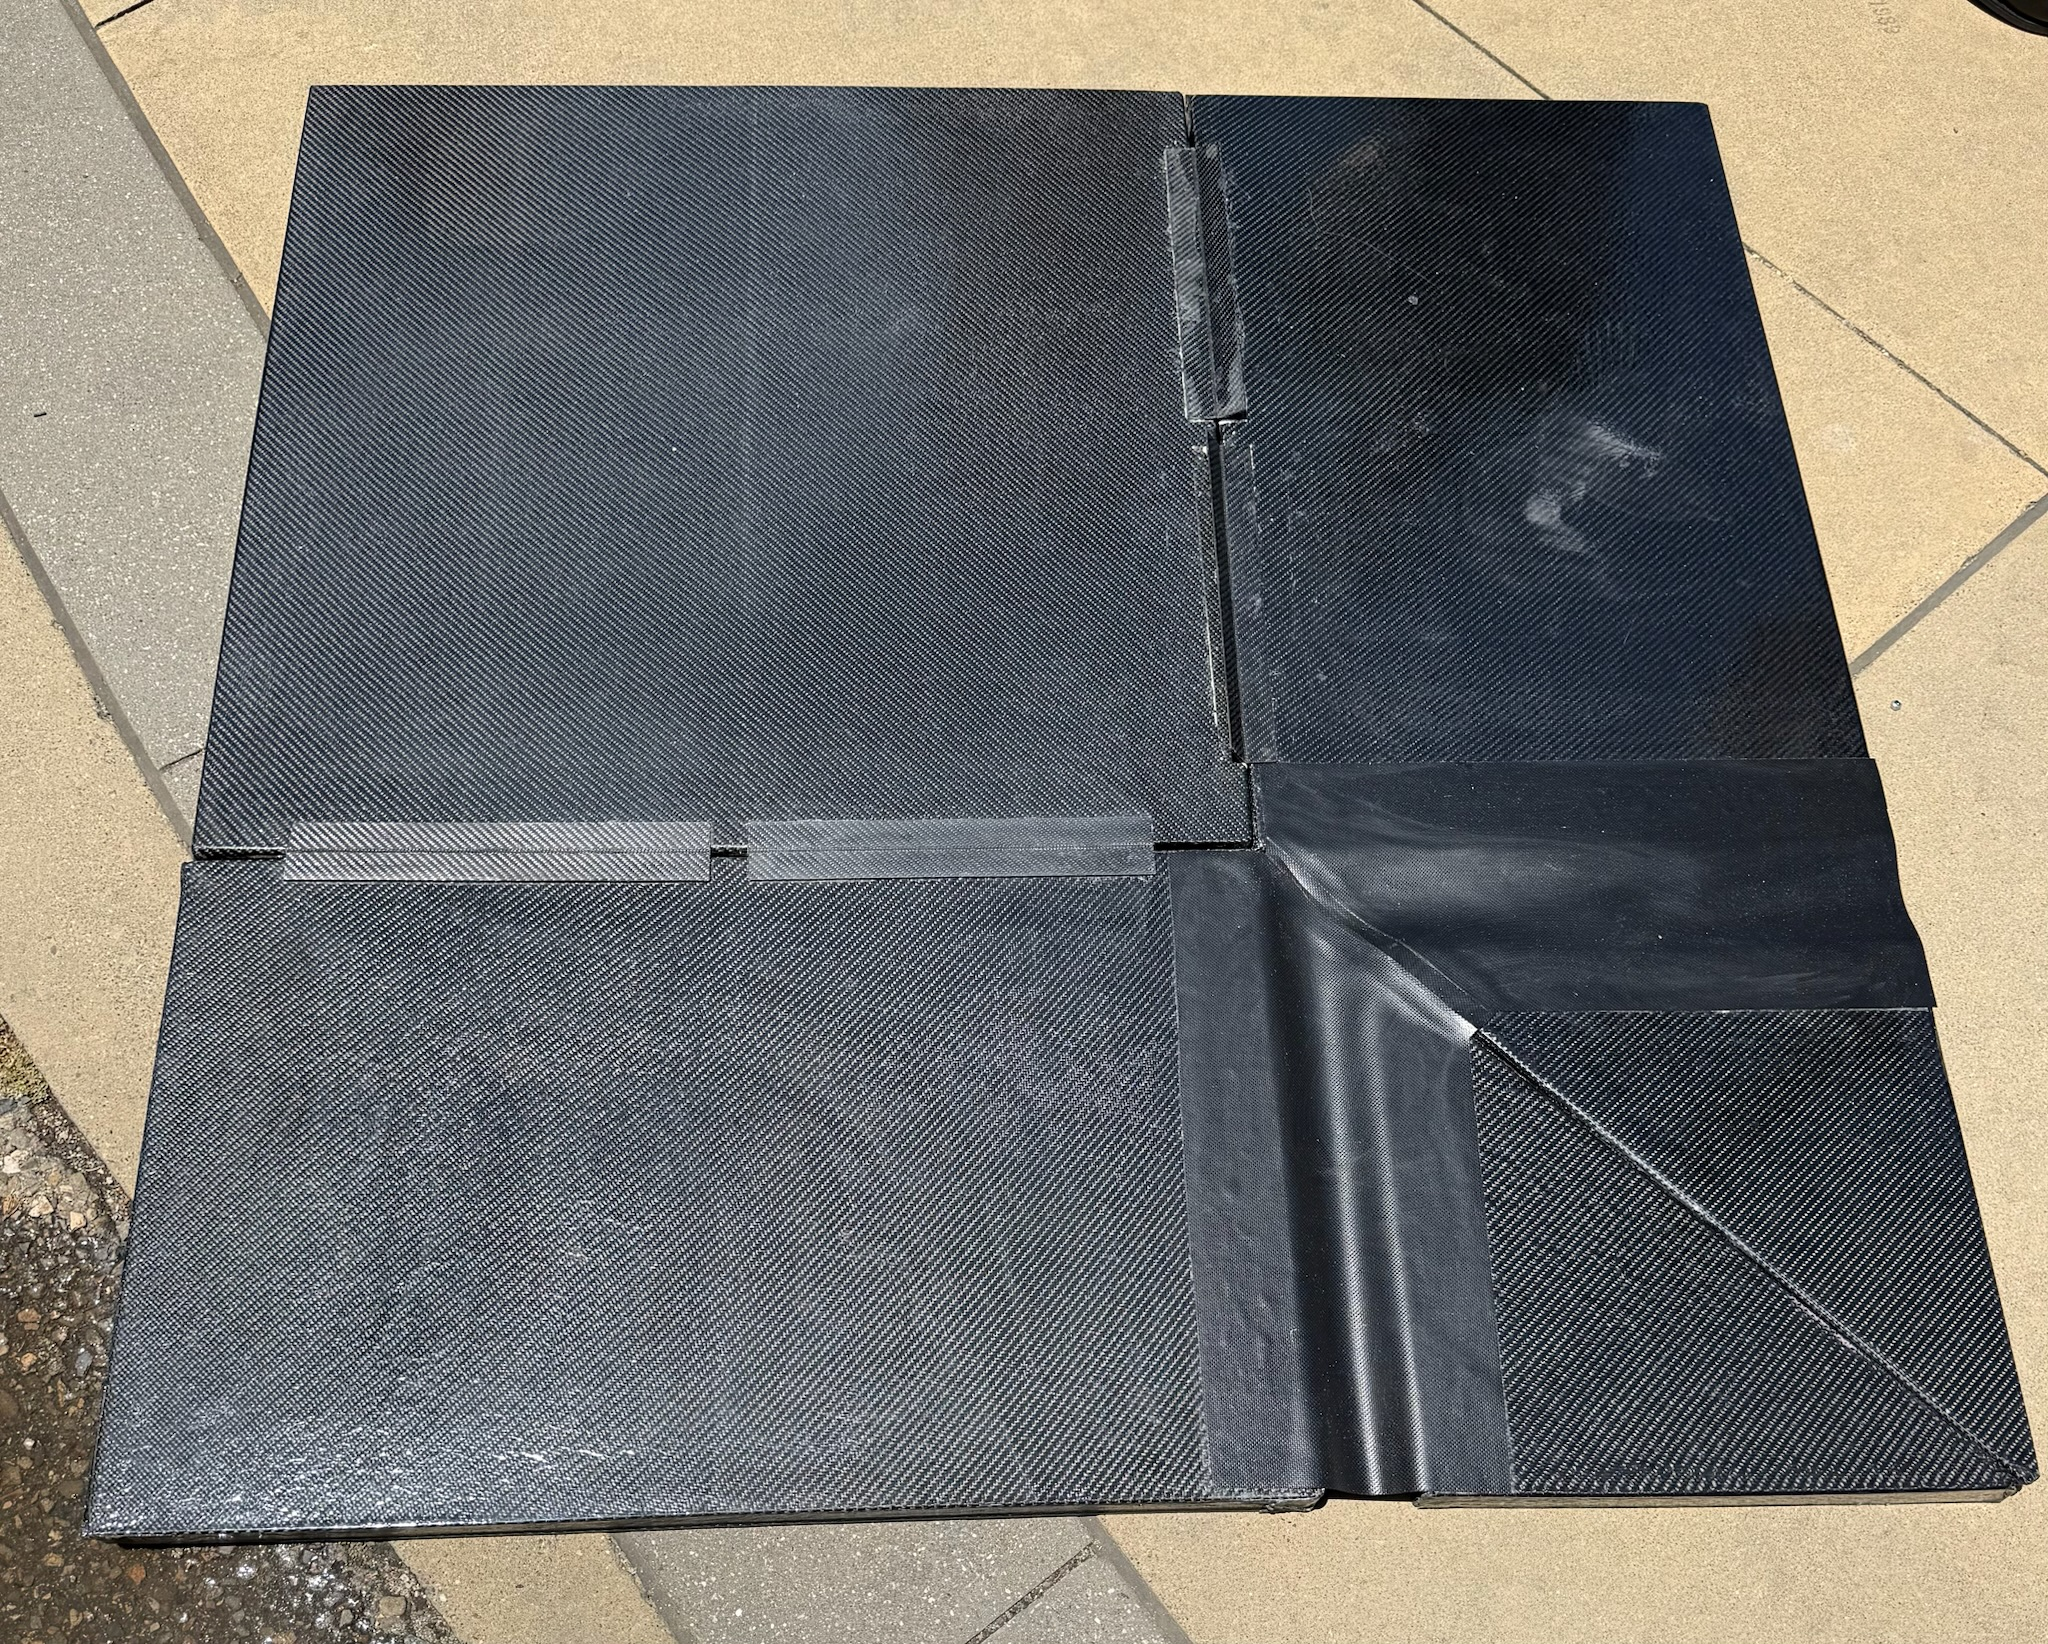
\includegraphics[
        width=2.35in,
        height=1.40in,
        keepaspectratio
    ]{refined_final_toro_cover_partial_carbon_model}
};
\draw[RuleGray,line width=0.55pt,rounded corners=4pt]
    ($(current page.north west)+(8.44in,-1.91in)$)
    rectangle
    ($(current page.north east)+(-0.42in,-3.40in)$);

% Captions
\node[anchor=north,text=Muted,font=\sffamily\fontsize{6.7}{7.3}\selectfont]
at ($(current page.north west)+(1.705in,-3.45in)$)
{Topcoat material preparation};

\node[anchor=north,text=Muted,font=\sffamily\fontsize{6.7}{7.3}\selectfont]
at ($(current page.north west)+(4.375in,-3.45in)$)
{Automotive-booth topcoat application};

\node[anchor=north,text=Muted,font=\sffamily\fontsize{6.7}{7.3}\selectfont]
at ($(current page.north west)+(7.045in,-3.45in)$)
{Coated panels drying after application};

\node[anchor=north,text=Muted,font=\sffamily\fontsize{6.7}{7.3}\selectfont]
at ($(current page.north west)+(9.50in,-3.45in)$)
{Partial carbon manufacturing model};

% Environmental rationale
\fill[SoftGold,rounded corners=4pt]
    ($(current page.north west)+(0.43in,-3.73in)$)
    rectangle
    ($(current page.north east)+(-0.42in,-4.76in)$);

\node[
    anchor=north west,
    align=left,
    text width=9.75in,
    text=Ink,
    font=\fontsize{7.05}{8.25}\selectfont
]
at ($(current page.north west)+(0.65in,-3.89in)$)
{
Because the sponsor required a carbon-fiber cover for outdoor use near chlorinated water,
environmental protection became a functional requirement rather than a cosmetic finish.
I selected and personally sprayed a UV-resistant Sunshield topcoat to seal minor laminate
porosity, reduce moisture ingress, preserve the carbon appearance, limit UV degradation of
the epoxy matrix, and isolate the composite surface from nearby metallic hardware.
};

% Results title
\node[
    anchor=north west,
    text=DeepGreen,
    font=\sffamily\bfseries\fontsize{8.0}{8.7}\selectfont
]
at ($(current page.north west)+(0.43in,-4.94in)$)
{FUNCTIONAL PROTOTYPE RESULTS};

% ------------------------------------------------------------
% Matched lower panels — larger type and improved allocation
% ------------------------------------------------------------

% Left results panel
\fill[SoftGreen,rounded corners=5pt]
    ($(current page.north west)+(0.43in,-5.22in)$)
    rectangle
    ($(current page.north west)+(5.98in,-7.39in)$);

\draw[RuleGray,line width=0.65pt,rounded corners=5pt]
    ($(current page.north west)+(0.43in,-5.22in)$)
    rectangle
    ($(current page.north west)+(5.98in,-7.39in)$);

\fill[DeepGreen,rounded corners=5pt]
    ($(current page.north west)+(0.43in,-5.22in)$)
    rectangle
    ($(current page.north west)+(5.98in,-5.58in)$);

\fill[DeepGreen]
    ($(current page.north west)+(0.43in,-5.40in)$)
    rectangle
    ($(current page.north west)+(5.98in,-5.58in)$);

\node[anchor=west,text=white,
      font=\sffamily\bfseries\fontsize{7.0}{7.6}\selectfont]
at ($(current page.north west)+(0.66in,-5.40in)$)
{SPECIFICATION};

\node[anchor=west,text=white,
      font=\sffamily\bfseries\fontsize{7.0}{7.6}\selectfont]
at ($(current page.north west)+(3.02in,-5.40in)$)
{RESULT};

\node[anchor=east,text=white,
      font=\sffamily\bfseries\fontsize{7.0}{7.6}\selectfont]
at ($(current page.north west)+(5.55in,-5.40in)$)
{STATUS};

\node[
    anchor=north west,
    align=left,
    text width=2.15in,
    text=Ink,
    font=\bfseries\fontsize{7.15}{8.55}\selectfont
]
at ($(current page.north west)+(0.66in,-5.72in)$)
{
Deployment time\\[3.4pt]
Removal time\\[3.4pt]
Single-user operation\\[3.4pt]
Single-side operation\\[3.4pt]
Deployment steps\\[3.4pt]
Removal steps\\[3.4pt]
Weight\\[3.4pt]
Folded storage
};

\node[
    anchor=north west,
    align=left,
    text width=1.45in,
    text=Ink,
    font=\fontsize{7.15}{8.55}\selectfont
]
at ($(current page.north west)+(3.02in,-5.72in)$)
{
25.51 seconds\\[3.4pt]
37.22 seconds\\[3.4pt]
100\% successful\\[3.4pt]
75\% successful\\[3.4pt]
6.4 average\\[3.4pt]
9 average\\[3.4pt]
17 lb\\[3.4pt]
2.9' x 2.9' x 1.7'
};

\node[
    anchor=north east,
    align=right,
    text width=1.05in,
    text=DeepGreen,
    font=\sffamily\bfseries\fontsize{7.05}{8.55}\selectfont
]
at ($(current page.north west)+(5.55in,-5.72in)$)
{
PASS\\[3.4pt]
PASS\\[3.4pt]
PASS\\[3.4pt]
NEAR TARGET\\[3.4pt]
PASS\\[3.4pt]
PASS\\[3.4pt]
NEAR TARGET\\[3.4pt]
PASS
};

% Right takeaways panel — widened for easier reading
\fill[SoftGreen,rounded corners=5pt]
    ($(current page.north west)+(6.14in,-5.22in)$)
    rectangle
    ($(current page.north east)+(-0.42in,-7.39in)$);

\draw[RuleGray,line width=0.65pt,rounded corners=5pt]
    ($(current page.north west)+(6.14in,-5.22in)$)
    rectangle
    ($(current page.north east)+(-0.42in,-7.39in)$);

\fill[DeepGreen,rounded corners=5pt]
    ($(current page.north west)+(6.14in,-5.22in)$)
    rectangle
    ($(current page.north east)+(-0.42in,-5.58in)$);

\fill[DeepGreen]
    ($(current page.north west)+(6.14in,-5.40in)$)
    rectangle
    ($(current page.north east)+(-0.42in,-5.58in)$);

\node[anchor=west,text=white,
      font=\sffamily\bfseries\fontsize{7.1}{7.7}\selectfont]
at ($(current page.north west)+(6.38in,-5.40in)$)
{ENGINEERING TAKEAWAYS};

\node[
    anchor=north west,
    align=left,
    text width=4.02in,
    text=Ink,
    font=\fontsize{6.75}{7.85}\selectfont
]
at ($(current page.north west)+(6.38in,-5.72in)$)
{
\textbf{Manufacturing first.}
Composite manufacturing constraints should guide the product architecture from the beginning.\\[4.5pt]
\textbf{Prioritize deliberately.}
Competing requirements must be balanced intentionally instead of maximizing every objective.\\[4.5pt]
\textbf{Lead through the process.}
Clear procedures, calm communication, and respect for teammates' strengths were essential during fabrication.\\[4.5pt]
\textbf{Next iteration.}
Reduce weight, refine the fabric-hinge fold lines, and improve panel-edge clearance.
};

% Compact concluding pathway
\node[
    anchor=center,
    align=center,
    text=PolyGold,
    font=\sffamily\bfseries\fontsize{6.3}{6.9}\selectfont
]
at ($(current page.north)+(3.06in,-7.18in)$)
{PROTOTYPE \faArrowRight\ DESIGN REFINEMENT
\faArrowRight\ REPEATABLE MANUFACTURING
\faArrowRight\ PRODUCT};

% Validation resources
\node[
    anchor=north,
    align=center,
    text=DeepGreen,
    font=\sffamily\bfseries\fontsize{6.6}{7.2}\selectfont
]
at ($(current page.north)+(0,-7.58in)$)
{\href{\ToroDeploymentLink}{\faPlayCircle\ DEPLOYMENT}
\hspace{18pt}
\href{\ToroRemovalLink}{\faPlayCircle\ REMOVAL / FOLDING}
\hspace{18pt}
\href{\ToroPosterLink}{\faFilePdf\ EXPO POSTER}
\hspace{18pt}
\href{\ToroReportLink}{\faFilePdf\ FINAL REPORT}};

% Footer
\node[
    anchor=south west,
    text=white,
    font=\sffamily\bfseries\fontsize{7.1}{7.7}\selectfont
]
at ($(current page.south west)+(0.42in,0.17in)$)
{\faArrowLeft\ MANUFACTURING-DRIVEN DESIGN};

\node[
    anchor=south,
    text=white,
    font=\sffamily\fontsize{7.0}{7.6}\selectfont
]
at ($(current page.south)+(0,0.17in)$)
{TORO COVER \hspace{6pt} 3 / 3};

\node[
    anchor=south east,
    text=white,
    font=\sffamily\bfseries\fontsize{7.1}{7.7}\selectfont
]
at ($(current page.south east)+(-0.42in,0.17in)$)
{NEXT PROJECT \faArrowRight};

\end{tikzpicture}
\input{paddle}
\clearpage
 before \end{document}.
% 3. Image references use the original Overleaf base filenames
%    without extensions.
% ============================================================



% ============================================================
% CLICKABLE PROJECT RESOURCES
% All links use the exact Google Drive resources supplied.
% ============================================================
\providecommand{\ToroDrawingLink}{https://drive.google.com/file/d/1A7-7wMnRNLuQDaTgxeuUCBsGNqyXzOGV/view?usp=sharing}
\providecommand{\ToroDimensionsLink}{https://drive.google.com/file/d/13sw3BNJvE8GdzlRffxoF2n5r9Gzxide7/view?usp=sharing}
\providecommand{\ToroProblemLink}{https://drive.google.com/file/d/1zHtl8zrb13F1yeN74ptawpfS5UM_xsuw/view?usp=drive_link}
\providecommand{\ToroReportLink}{https://drive.google.com/file/d/1ULZ-P46lFsC2x29ZfmRVIKgYnr9o8hMt/view?usp=drive_link}
\providecommand{\ToroPosterLink}{https://drive.google.com/file/d/1vKiKaJUcHQb_db-FkZnRF6EvtuM4hKyS/view?usp=drive_link}
\providecommand{\ToroDeploymentLink}{https://drive.google.com/file/d/1XJx34o80_mZPTl7xy93HtWAgtS3ThhvY/view?usp=drive_link}
\providecommand{\ToroRemovalLink}{https://drive.google.com/file/d/1O7xYeyB67NUwT-j1B1HeiCcHnZDYjk6_/view?usp=drive_link}

% ============================================================
% PAGE 1 — PROJECT OVERVIEW, OWNERSHIP, AND ARCHITECTURE
% ============================================================

\clearpage
\thispagestyle{empty}
\hypertarget{toro}{}
\null

\begin{tikzpicture}[remember picture,overlay]

% Background
\fill[white]
    (current page.south west)
    rectangle
    (current page.north east);

% Page bars
\fill[DeepGreen]
    (current page.north west)
    rectangle
    ($(current page.north east)+(0,-0.095in)$);

\fill[PolyGold]
    ($(current page.north west)+(0,-0.095in)$)
    rectangle
    ($(current page.north east)+(0,-0.14in)$);

\fill[DeepGreen]
    (current page.south west)
    rectangle
    ($(current page.south east)+(0,0.36in)$);

\fill[PolyGold]
    ($(current page.south west)+(0,0.36in)$)
    rectangle
    ($(current page.south east)+(0,0.405in)$);

% Header
\node[
    anchor=north west,
    text=PolyGold,
    font=\sffamily\bfseries\fontsize{8.1}{8.7}\selectfont
]
at ($(current page.north west)+(0.42in,-0.39in)$)
{01 COMPOSITES \hspace{5pt}/\hspace{5pt} PROJECT 01};

\node[
    anchor=north west,
    text=DeepGreen,
    font=\bfseries\fontsize{23.5}{24.5}\selectfont
]
at ($(current page.north west)+(0.40in,-0.67in)$)
{TORO CARBON FIBER SAFETY COVER};

\node[
    anchor=north west,
    text=Muted,
    font=\sffamily\fontsize{8.4}{9.2}\selectfont
]
at ($(current page.north west)+(0.42in,-1.12in)$)
{Cal Poly Composites Laboratory \hspace{7pt}\textbullet\hspace{7pt}
Team Project \hspace{7pt}\textbullet\hspace{7pt}
Fall--Spring 2026 \hspace{7pt}\textbullet\hspace{7pt}
San Luis Obispo, California};

\fill[PolyGold]
    ($(current page.north west)+(0.42in,-1.37in)$)
    rectangle
    ($(current page.north west)+(6.1in,-1.325in)$);

% Challenge text
\node[
    anchor=north west,
    text=DeepGreen,
    font=\sffamily\bfseries\fontsize{8.1}{8.8}\selectfont
]
at ($(current page.north west)+(0.43in,-1.61in)$)
{THE CHALLENGE};

\node[
    anchor=north west,
    align=left,
    text width=4.47in,
    text=Ink,
    font=\fontsize{8.05}{9.65}\selectfont
]
at ($(current page.north west)+(0.43in,-1.84in)$)
{
Develop a lightweight cover for a 6 ft by 6 ft in-ground spa
that could be deployed by one person, stored compactly,
provide insulation, resist a poolside environment, and maintain
a refined appearance. The sponsor supplied an ambitious but
intentionally broad project statement, requiring the team to
define the product architecture, priorities, manufacturing
strategy, and realistic path toward future commercialization.
};

% Role box
\fill[SoftGold,rounded corners=5pt]
    ($(current page.north west)+(0.42in,-2.88in)$)
    rectangle
    ($(current page.north west)+(4.98in,-4.58in)$);

\fill[PolyGold]
    ($(current page.north west)+(0.42in,-2.88in)$)
    rectangle
    ($(current page.north west)+(0.52in,-4.58in)$);

\node[
    anchor=north west,
    text=DeepGreen,
    font=\sffamily\bfseries\fontsize{8.1}{8.8}\selectfont
]
at ($(current page.north west)+(0.66in,-3.02in)$)
{MY ROLE — DESIGN \& MANUFACTURING LEAD};

\node[
    anchor=north west,
    align=left,
    text width=4.02in,
    text=Ink,
    font=\fontsize{7.05}{8.15}\selectfont
]
at ($(current page.north west)+(0.66in,-3.27in)$)
{
\textbullet\ Modeled every custom part and the complete assembly\\[1.5pt]
\textbullet\ Produced the engineering drawing package independently\\[1.5pt]
\textbullet\ Developed the composite-panel manufacturing process\\[1.5pt]
\textbullet\ Created all waterjet DXFs and manufacturing geometry\\[1.5pt]
\textbullet\ Trained teammates in wet layup and vacuum bagging\\[1.5pt]
\textbullet\ Presented feasibility, scope, and tradeoffs to the sponsor
};

% Large deployed foam-model image
\node[anchor=center,inner sep=0pt]
at ($(current page.north west)+(8.00in,-3.04in)$)
{
    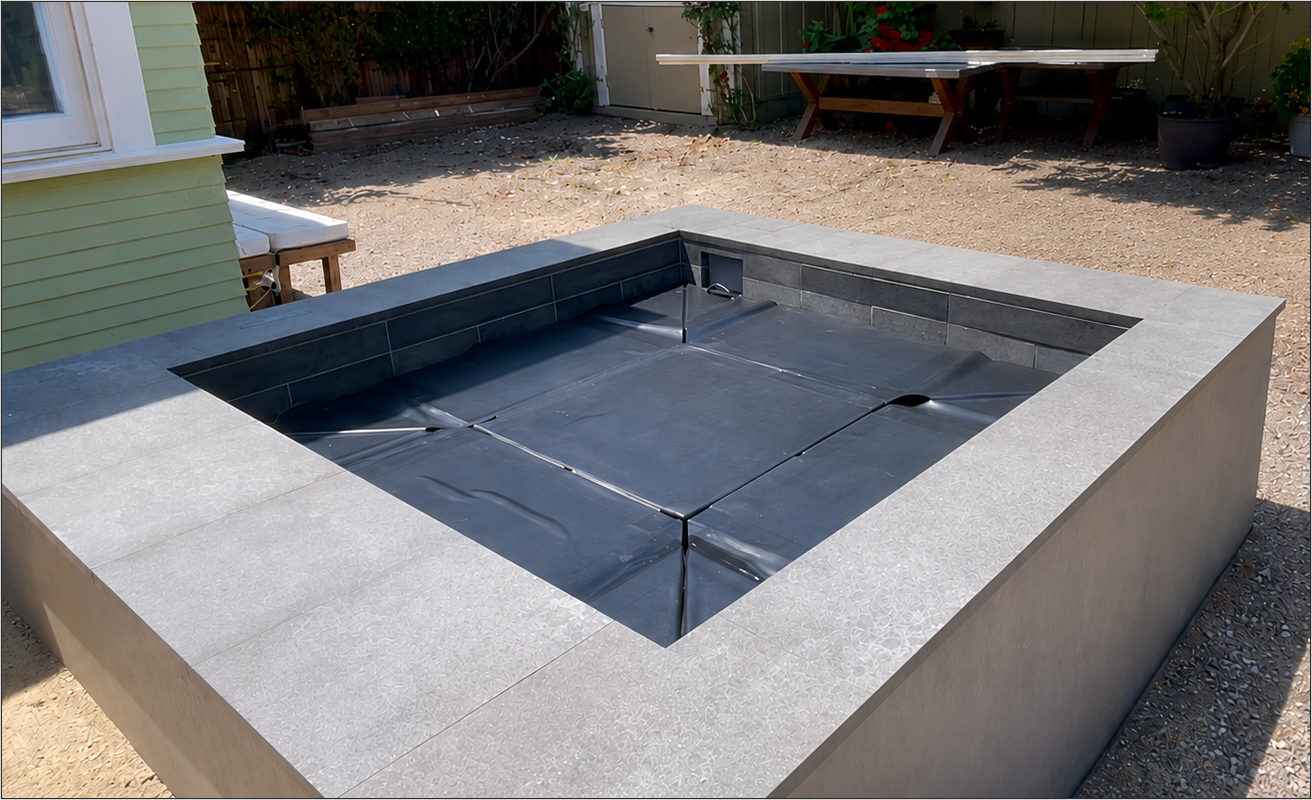
\includegraphics[
        width=5.55in,
        height=2.78in,
        keepaspectratio
    ]{deployed_functional_prototype}
};

\draw[DeepGreen,line width=0.8pt,rounded corners=7pt]
    ($(current page.north west)+(5.16in,-1.61in)$)
    rectangle
    ($(current page.north east)+(-0.42in,-4.47in)$);

\node[
    anchor=north west,
    text=Muted,
    font=\sffamily\fontsize{6.2}{6.9}\selectfont
]
at ($(current page.north west)+(5.18in,-4.54in)$)
{Functional foam model deployed over the sponsor's in-ground spa.};

% Image-strip title
\node[
    anchor=north west,
    text=DeepGreen,
    font=\sffamily\bfseries\fontsize{8.1}{8.8}\selectfont
]
at ($(current page.north west)+(0.43in,-4.78in)$)
{PRODUCT DEVELOPMENT AND FINAL ARCHITECTURE};

% Five-image development strip — CAD-first sequence
% Image 1: topside CAD
\node[anchor=center,inner sep=0pt]
at ($(current page.north west)+(1.47in,-5.73in)$)
{
    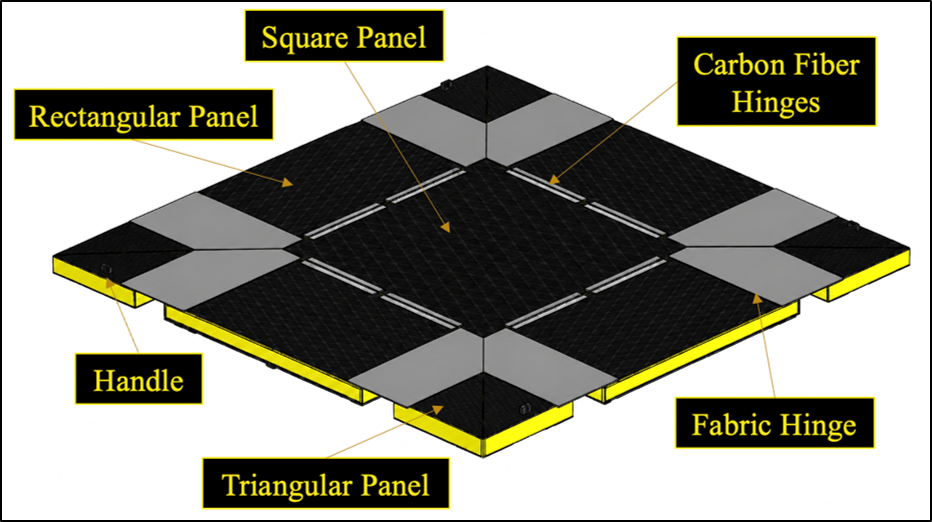
\includegraphics[
        width=1.92in,
        height=1.30in,
        keepaspectratio
    ]{Toro_Cover_topside_Cad}
};
\draw[RuleGray,line width=0.55pt,rounded corners=4pt]
    ($(current page.north west)+(0.43in,-5.04in)$)
    rectangle
    ($(current page.north west)+(2.51in,-6.43in)$);

% Image 2: underside CAD
\node[anchor=center,inner sep=0pt]
at ($(current page.north west)+(3.66in,-5.73in)$)
{
    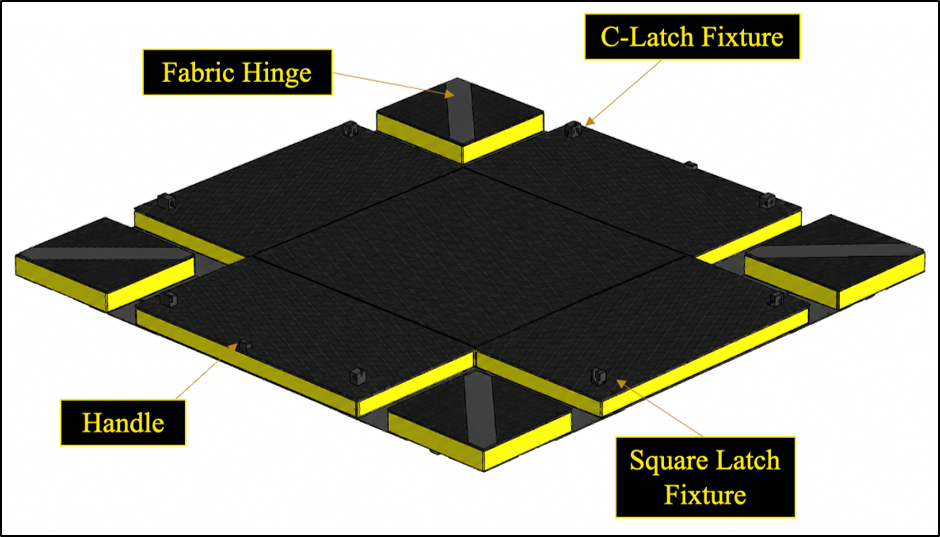
\includegraphics[
        width=1.92in,
        height=1.30in,
        keepaspectratio
    ]{toro_cover_underside_cad}
};
\draw[RuleGray,line width=0.55pt,rounded corners=4pt]
    ($(current page.north west)+(2.62in,-5.04in)$)
    rectangle
    ($(current page.north west)+(4.70in,-6.43in)$);

% Image 3: folded CAD
\node[anchor=center,inner sep=0pt]
at ($(current page.north west)+(5.85in,-5.73in)$)
{
    \includegraphics[
        width=1.92in,
        height=1.30in,
        keepaspectratio
    ]{\detokenize{Toro_Cover_folded Configuration}}
};
\draw[RuleGray,line width=0.55pt,rounded corners=4pt]
    ($(current page.north west)+(4.81in,-5.04in)$)
    rectangle
    ($(current page.north west)+(6.89in,-6.43in)$);

% Image 4: dual-use product concept
\node[anchor=center,inner sep=0pt]
at ($(current page.north west)+(8.04in,-5.73in)$)
{
    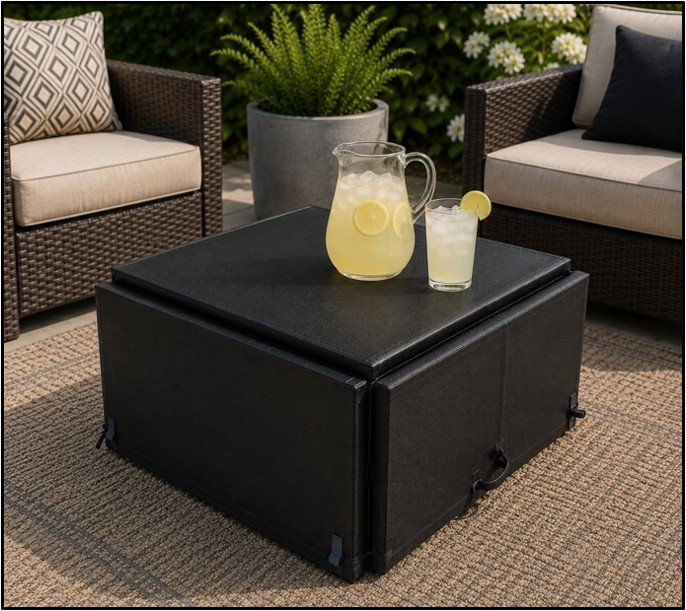
\includegraphics[
        width=1.92in,
        height=1.30in,
        keepaspectratio
    ]{generative_AI_concept_toro_cover_art}
};
\draw[RuleGray,line width=0.55pt,rounded corners=4pt]
    ($(current page.north west)+(7.00in,-5.04in)$)
    rectangle
    ($(current page.north west)+(9.08in,-6.43in)$);

% Image 5: folded foam functional prototype
% The portrait photograph is deliberately clipped to the landscape frame
% so the ottoman fills the card without extending beyond its border.
\begin{scope}
\clip[rounded corners=4pt]
    ($(current page.north west)+(9.19in,-5.04in)$)
    rectangle
    ($(current page.north east)+(-0.43in,-6.43in)$);

% Keep the original image proportions and center it within the existing card.
\node[anchor=center,inner sep=0pt]
at ($(current page.north west)+(9.88in,-5.735in)$)
{
    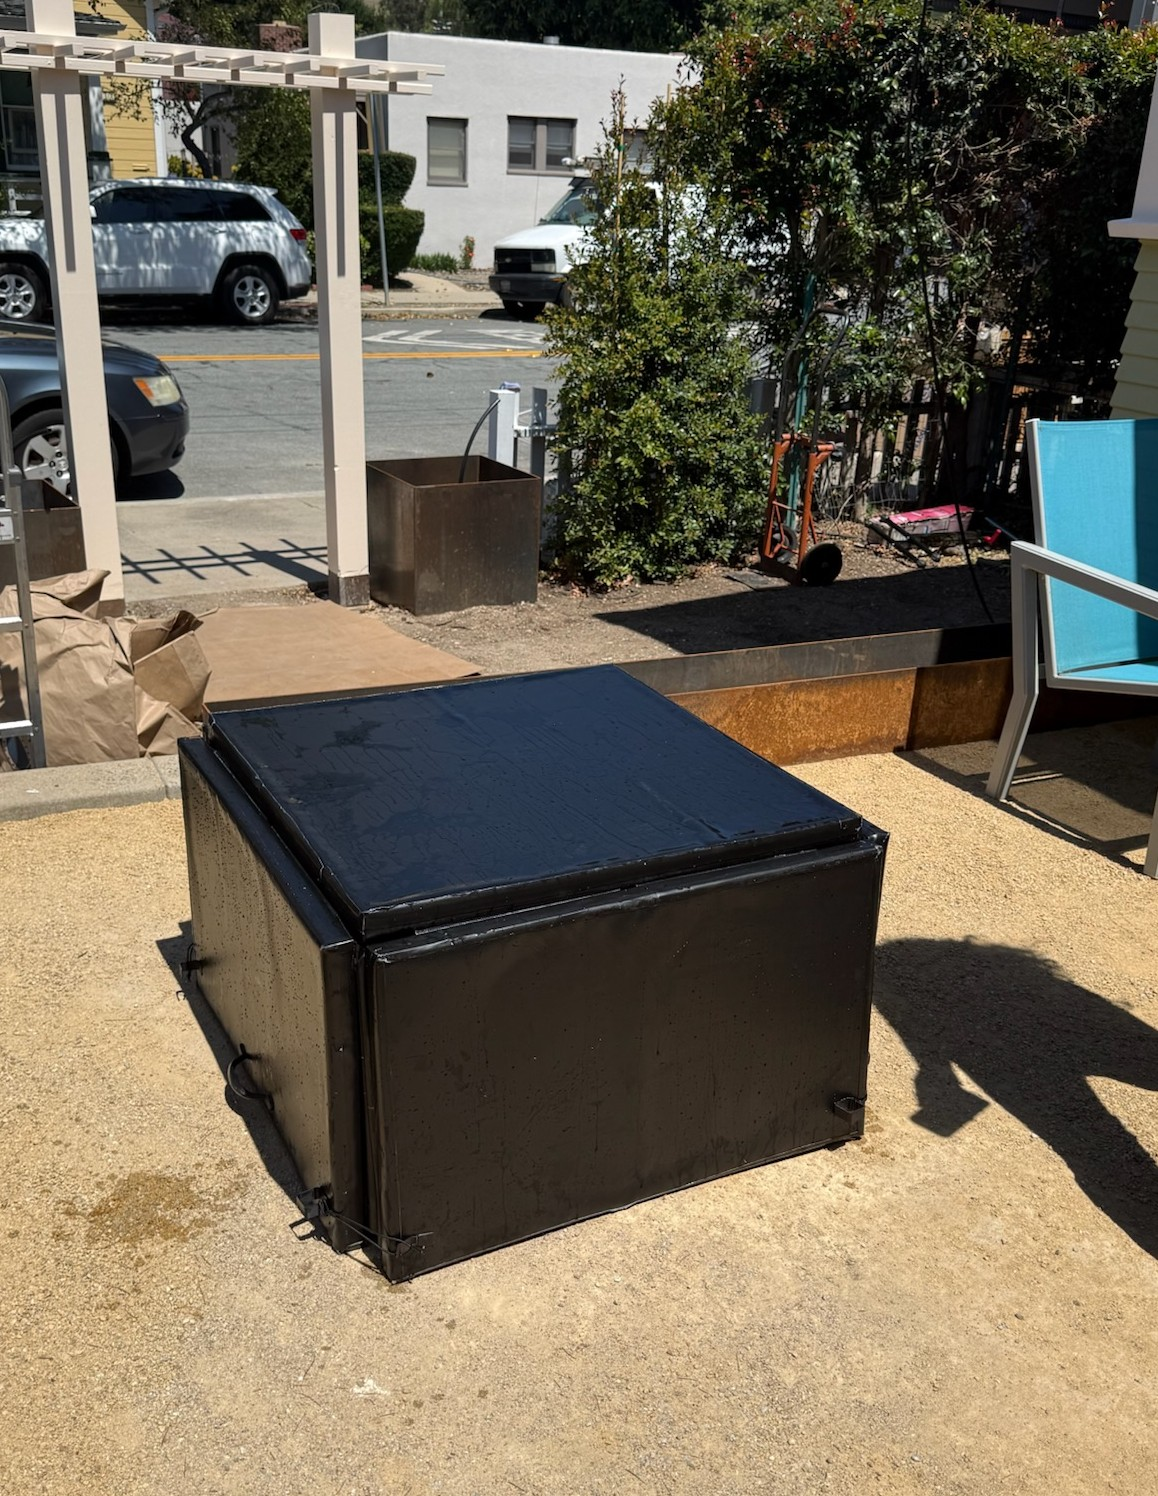
\includegraphics[
        width=1.58in,
        height=1.28in,
        keepaspectratio
    ]{foam_model_folded_backyard_image}
};
\end{scope}

\draw[RuleGray,line width=0.55pt,rounded corners=4pt]
    ($(current page.north west)+(9.19in,-5.04in)$)
    rectangle
    ($(current page.north east)+(-0.43in,-6.43in)$);

% Larger captions
\node[anchor=north,align=center,text width=1.95in,text=Muted,
      font=\sffamily\fontsize{6.8}{7.4}\selectfont]
at ($(current page.north west)+(1.47in,-6.49in)$)
{Topside panel architecture};

\node[anchor=north,align=center,text width=1.95in,text=Muted,
      font=\sffamily\fontsize{6.8}{7.4}\selectfont]
at ($(current page.north west)+(3.66in,-6.49in)$)
{Underside hinge architecture};

\node[anchor=north,align=center,text width=1.95in,text=Muted,
      font=\sffamily\fontsize{6.8}{7.4}\selectfont]
at ($(current page.north west)+(5.85in,-6.49in)$)
{Folded CAD configuration};

\node[anchor=north,align=center,text width=1.95in,text=Muted,
      font=\sffamily\fontsize{6.8}{7.4}\selectfont]
at ($(current page.north west)+(8.04in,-6.49in)$)
{Dual-use product vision};

\node[anchor=north,align=center,text width=1.95in,text=Muted,
      font=\sffamily\fontsize{6.8}{7.4}\selectfont]
at ($(current page.north west)+(9.88in,-6.49in)$)
{Folded foam prototype};

% Page 1 resource bar — centered and non-repeated resources
\fill[Panel,rounded corners=4pt]
    ($(current page.north west)+(0.43in,-7.05in)$)
    rectangle
    ($(current page.north east)+(-0.43in,-7.64in)$);
\draw[RuleGray,line width=0.5pt,rounded corners=4pt]
    ($(current page.north west)+(0.43in,-7.05in)$)
    rectangle
    ($(current page.north east)+(-0.43in,-7.64in)$);

\node[
    anchor=center,
    align=center,
    text=DeepGreen,
    font=\sffamily\bfseries\fontsize{6.9}{7.5}\selectfont
]
at ($(current page.north)+(0,-7.345in)$)
{\href{\ToroDrawingLink}{\faDraftingCompass\ DRAWING PACKAGE}
\hspace{24pt}
\href{\ToroDimensionsLink}{\faImage\ DIMENSION STUDY}
\hspace{24pt}
\href{\ToroProblemLink}{\faFileImage\ PROBLEM STATEMENT}};

% Footer
\node[
    anchor=south west,
    text=white,
    font=\sffamily\bfseries\fontsize{7.1}{7.7}\selectfont
]
at ($(current page.south west)+(0.42in,0.17in)$)
{\hyperlink{composites}{\faArrowLeft\ COMPOSITES}};

\node[
    anchor=south,
    text=white,
    font=\sffamily\fontsize{7.0}{7.6}\selectfont
]
at ($(current page.south)+(0,0.17in)$)
{TORO COVER \hspace{6pt} 1 / 3};

\node[
    anchor=south east,
    text=white,
    font=\sffamily\bfseries\fontsize{7.1}{7.7}\selectfont
]
at ($(current page.south east)+(-0.42in,0.17in)$)
{MANUFACTURING-DRIVEN DESIGN \faArrowRight};

\end{tikzpicture}


% ============================================================
% PAGE 2 — MANUFACTURING-DRIVEN DESIGN
% ============================================================

\clearpage
\thispagestyle{empty}
\hypertarget{toro-manufacturing}{}
\null

\begin{tikzpicture}[remember picture,overlay]

% Background and bars
\fill[white]
    (current page.south west)
    rectangle
    (current page.north east);

\fill[DeepGreen]
    (current page.north west)
    rectangle
    ($(current page.north east)+(0,-0.095in)$);

\fill[PolyGold]
    ($(current page.north west)+(0,-0.095in)$)
    rectangle
    ($(current page.north east)+(0,-0.14in)$);

\fill[DeepGreen]
    (current page.south west)
    rectangle
    ($(current page.south east)+(0,0.36in)$);

\fill[PolyGold]
    ($(current page.south west)+(0,0.36in)$)
    rectangle
    ($(current page.south east)+(0,0.405in)$);

% Header
\node[
    anchor=north west,
    text=PolyGold,
    font=\sffamily\bfseries\fontsize{8.1}{8.7}\selectfont
]
at ($(current page.north west)+(0.42in,-0.39in)$)
{TORO COVER \hspace{5pt}/\hspace{5pt} DESIGN FOR MANUFACTURABILITY};

\node[
    anchor=north west,
    text=DeepGreen,
    font=\bfseries\fontsize{23}{24}\selectfont
]
at ($(current page.north west)+(0.40in,-0.67in)$)
{THE ENVELOPE METHOD};

\node[
    anchor=north west,
    text=Muted,
    font=\sffamily\fontsize{8.7}{9.6}\selectfont
]
at ($(current page.north west)+(0.42in,-1.12in)$)
{A one-layup process developed for unusually thick insulated composite sandwich panels};

\fill[PolyGold]
    ($(current page.north west)+(0.42in,-1.36in)$)
    rectangle
    ($(current page.north west)+(5.30in,-1.315in)$);

% Process explanation
\fill[SoftGold,rounded corners=5pt]
    ($(current page.north west)+(0.42in,-1.61in)$)
    rectangle
    ($(current page.north east)+(-0.42in,-2.90in)$);

\fill[PolyGold]
    ($(current page.north west)+(0.42in,-1.61in)$)
    rectangle
    ($(current page.north west)+(0.52in,-2.90in)$);

\node[
    anchor=north west,
    text=DeepGreen,
    font=\sffamily\bfseries\fontsize{7.9}{8.6}\selectfont
]
at ($(current page.north west)+(0.67in,-1.76in)$)
{PROCESS INNOVATION};

\node[
    anchor=north west,
    align=left,
    text width=9.55in,
    text=Ink,
    font=\fontsize{7.35}{8.75}\selectfont
]
at ($(current page.north west)+(0.67in,-2.02in)$)
{
Weight reduction and insulation were both essential, leading to the selection of an
XPS foam core. Because XPS could not tolerate composite heat-cure temperatures, prepreg
processing was not practical and the panels had to be manufactured by wet layup with a
room-temperature cure. To simplify this process, I waterjet-cut XPS perimeter strips from
excess foam and placed them around each core inside the vacuum enclosure. Under vacuum,
the top and bottom carbon skins met along the panel sides and compressed against this
border, eliminating a separate edge-banding layup and reducing corner pleating.
};

% Workflow title
\node[
    anchor=north west,
    text=DeepGreen,
    font=\sffamily\bfseries\fontsize{8.0}{8.7}\selectfont
]
at ($(current page.north west)+(0.43in,-3.06in)$)
{MANUFACTURING WORKFLOW};

% Row 1 image 1
\node[anchor=center,inner sep=0pt]
at ($(current page.north west)+(2.07in,-4.105in)$)
{
    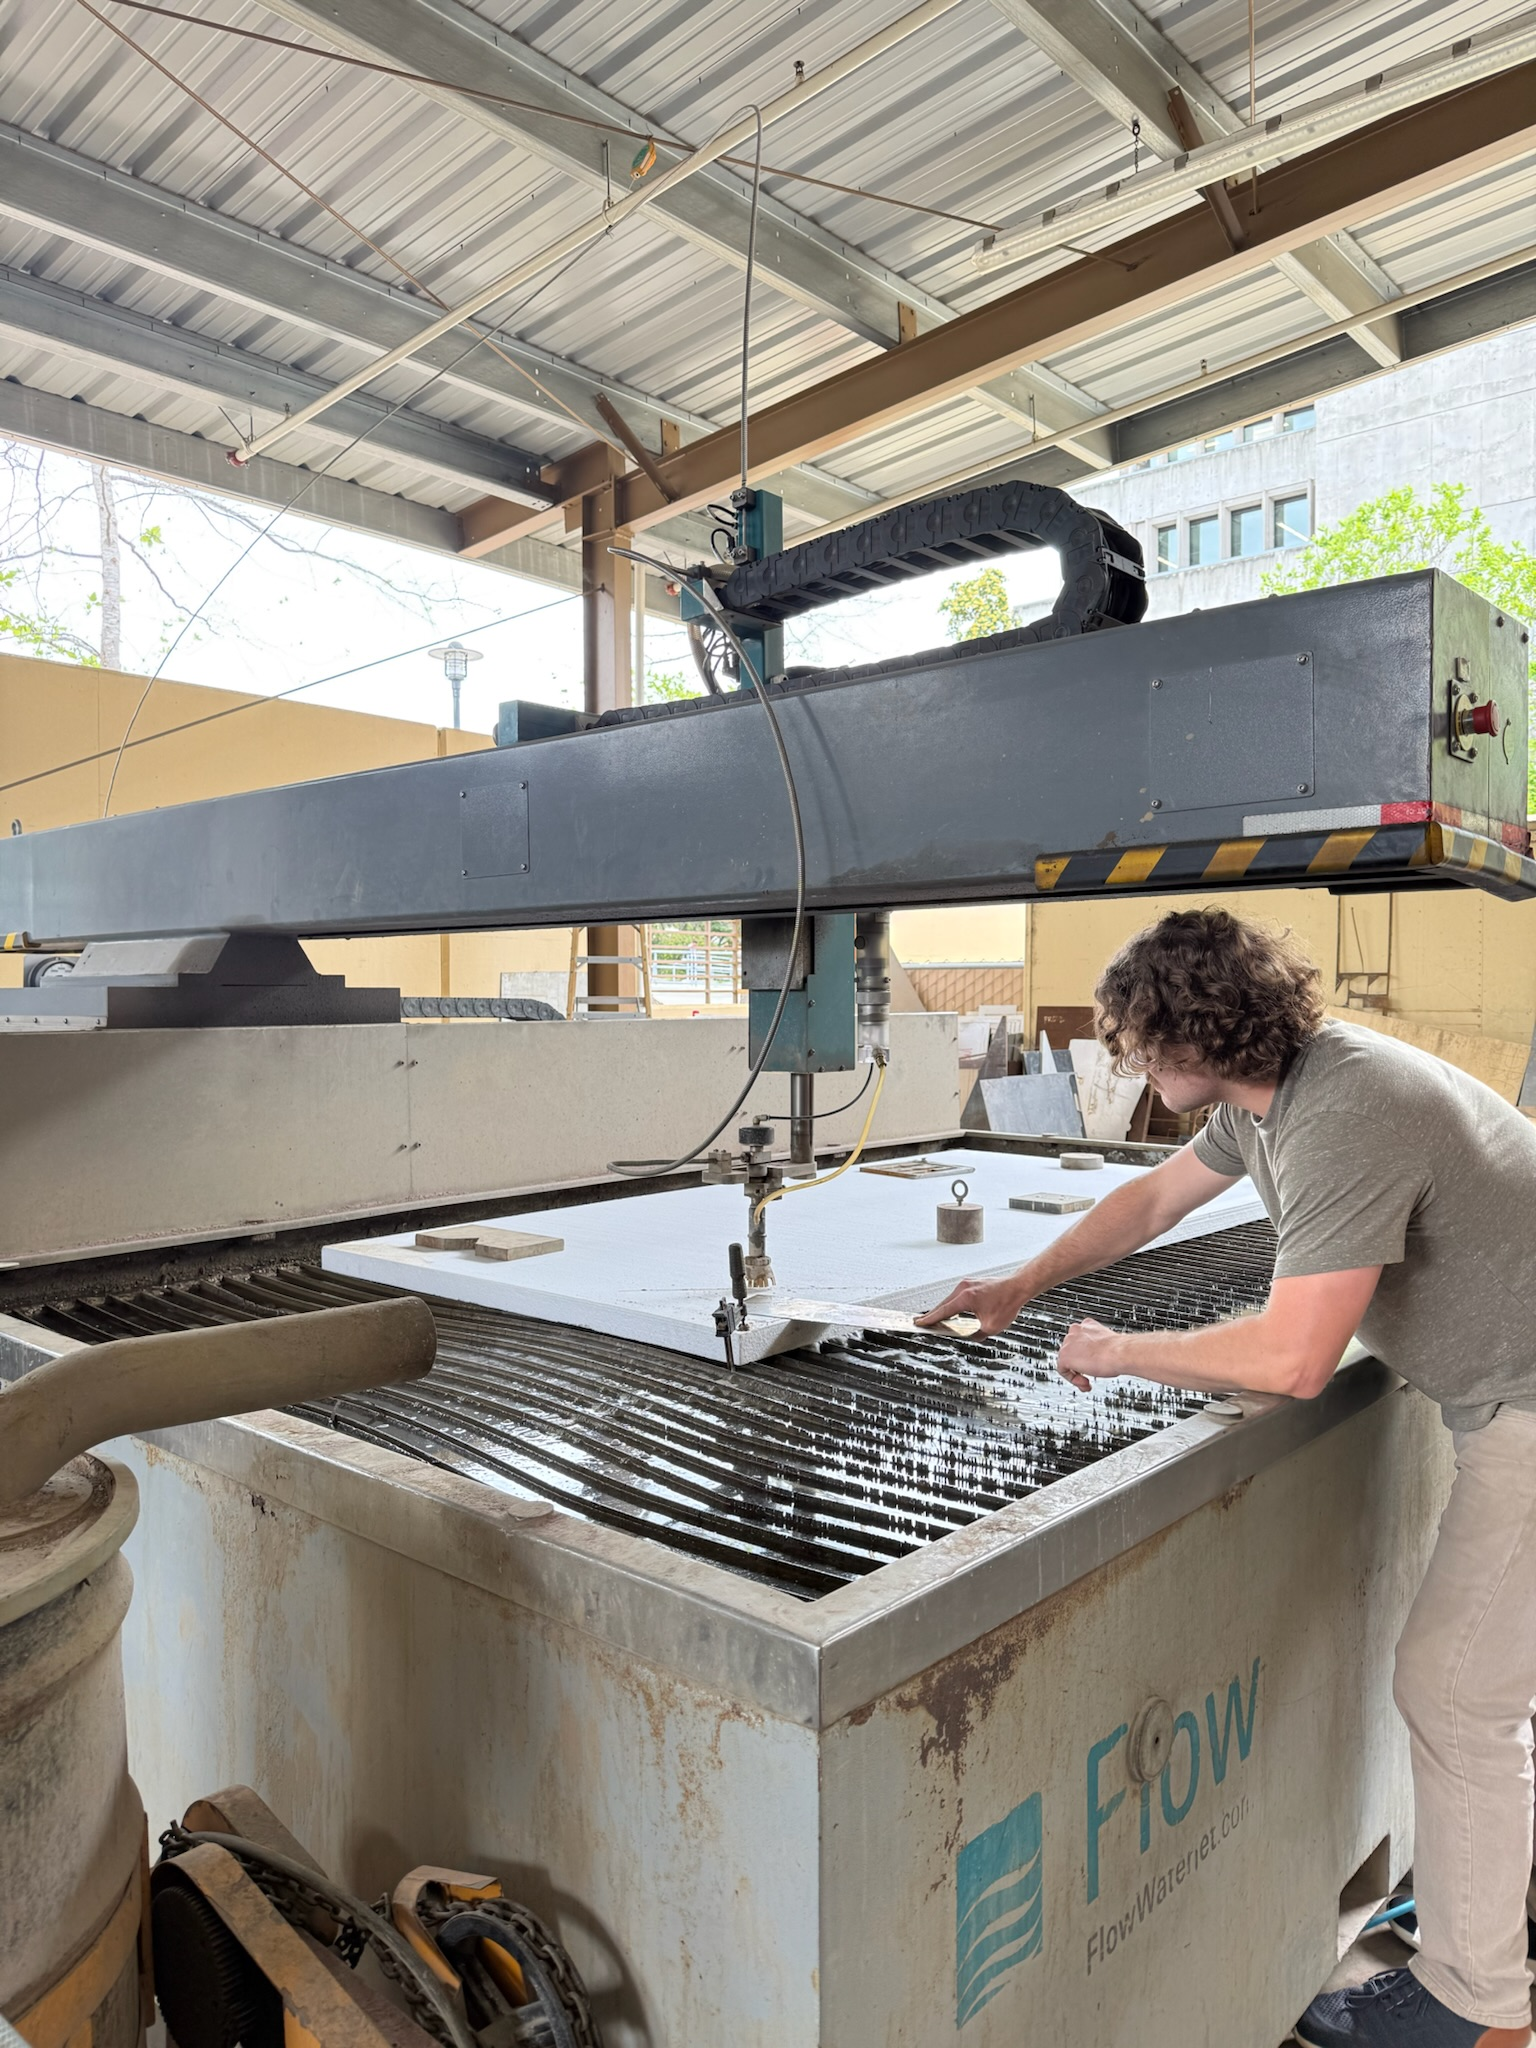
\includegraphics[
        width=3.10in,
        height=1.40in,
        keepaspectratio
    ]{waterjet_foam}
};
\draw[RuleGray,line width=0.55pt,rounded corners=4pt]
    ($(current page.north west)+(0.43in,-3.36in)$)
    rectangle
    ($(current page.north west)+(3.71in,-4.85in)$);

% Row 1 image 2
\node[anchor=center,inner sep=0pt]
at ($(current page.north west)+(5.50in,-4.105in)$)
{
    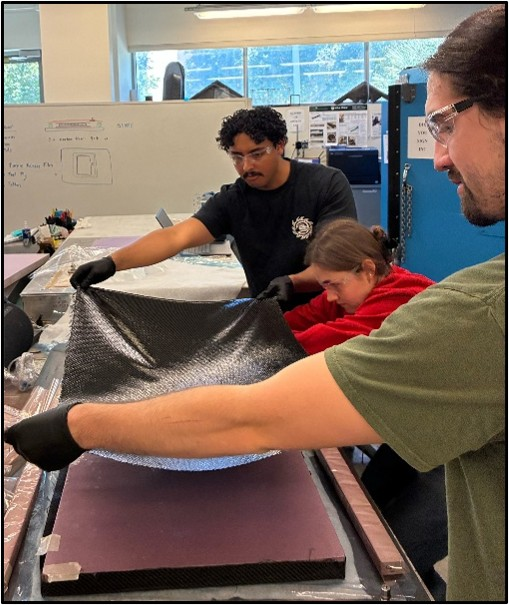
\includegraphics[
        width=3.10in,
        height=1.40in,
        keepaspectratio
    ]{group_layup}
};
\draw[RuleGray,line width=0.55pt,rounded corners=4pt]
    ($(current page.north west)+(3.86in,-3.36in)$)
    rectangle
    ($(current page.north west)+(7.14in,-4.85in)$);

% Row 1 image 3
\node[anchor=center,inner sep=0pt]
at ($(current page.north west)+(8.935in,-4.105in)$)
{
    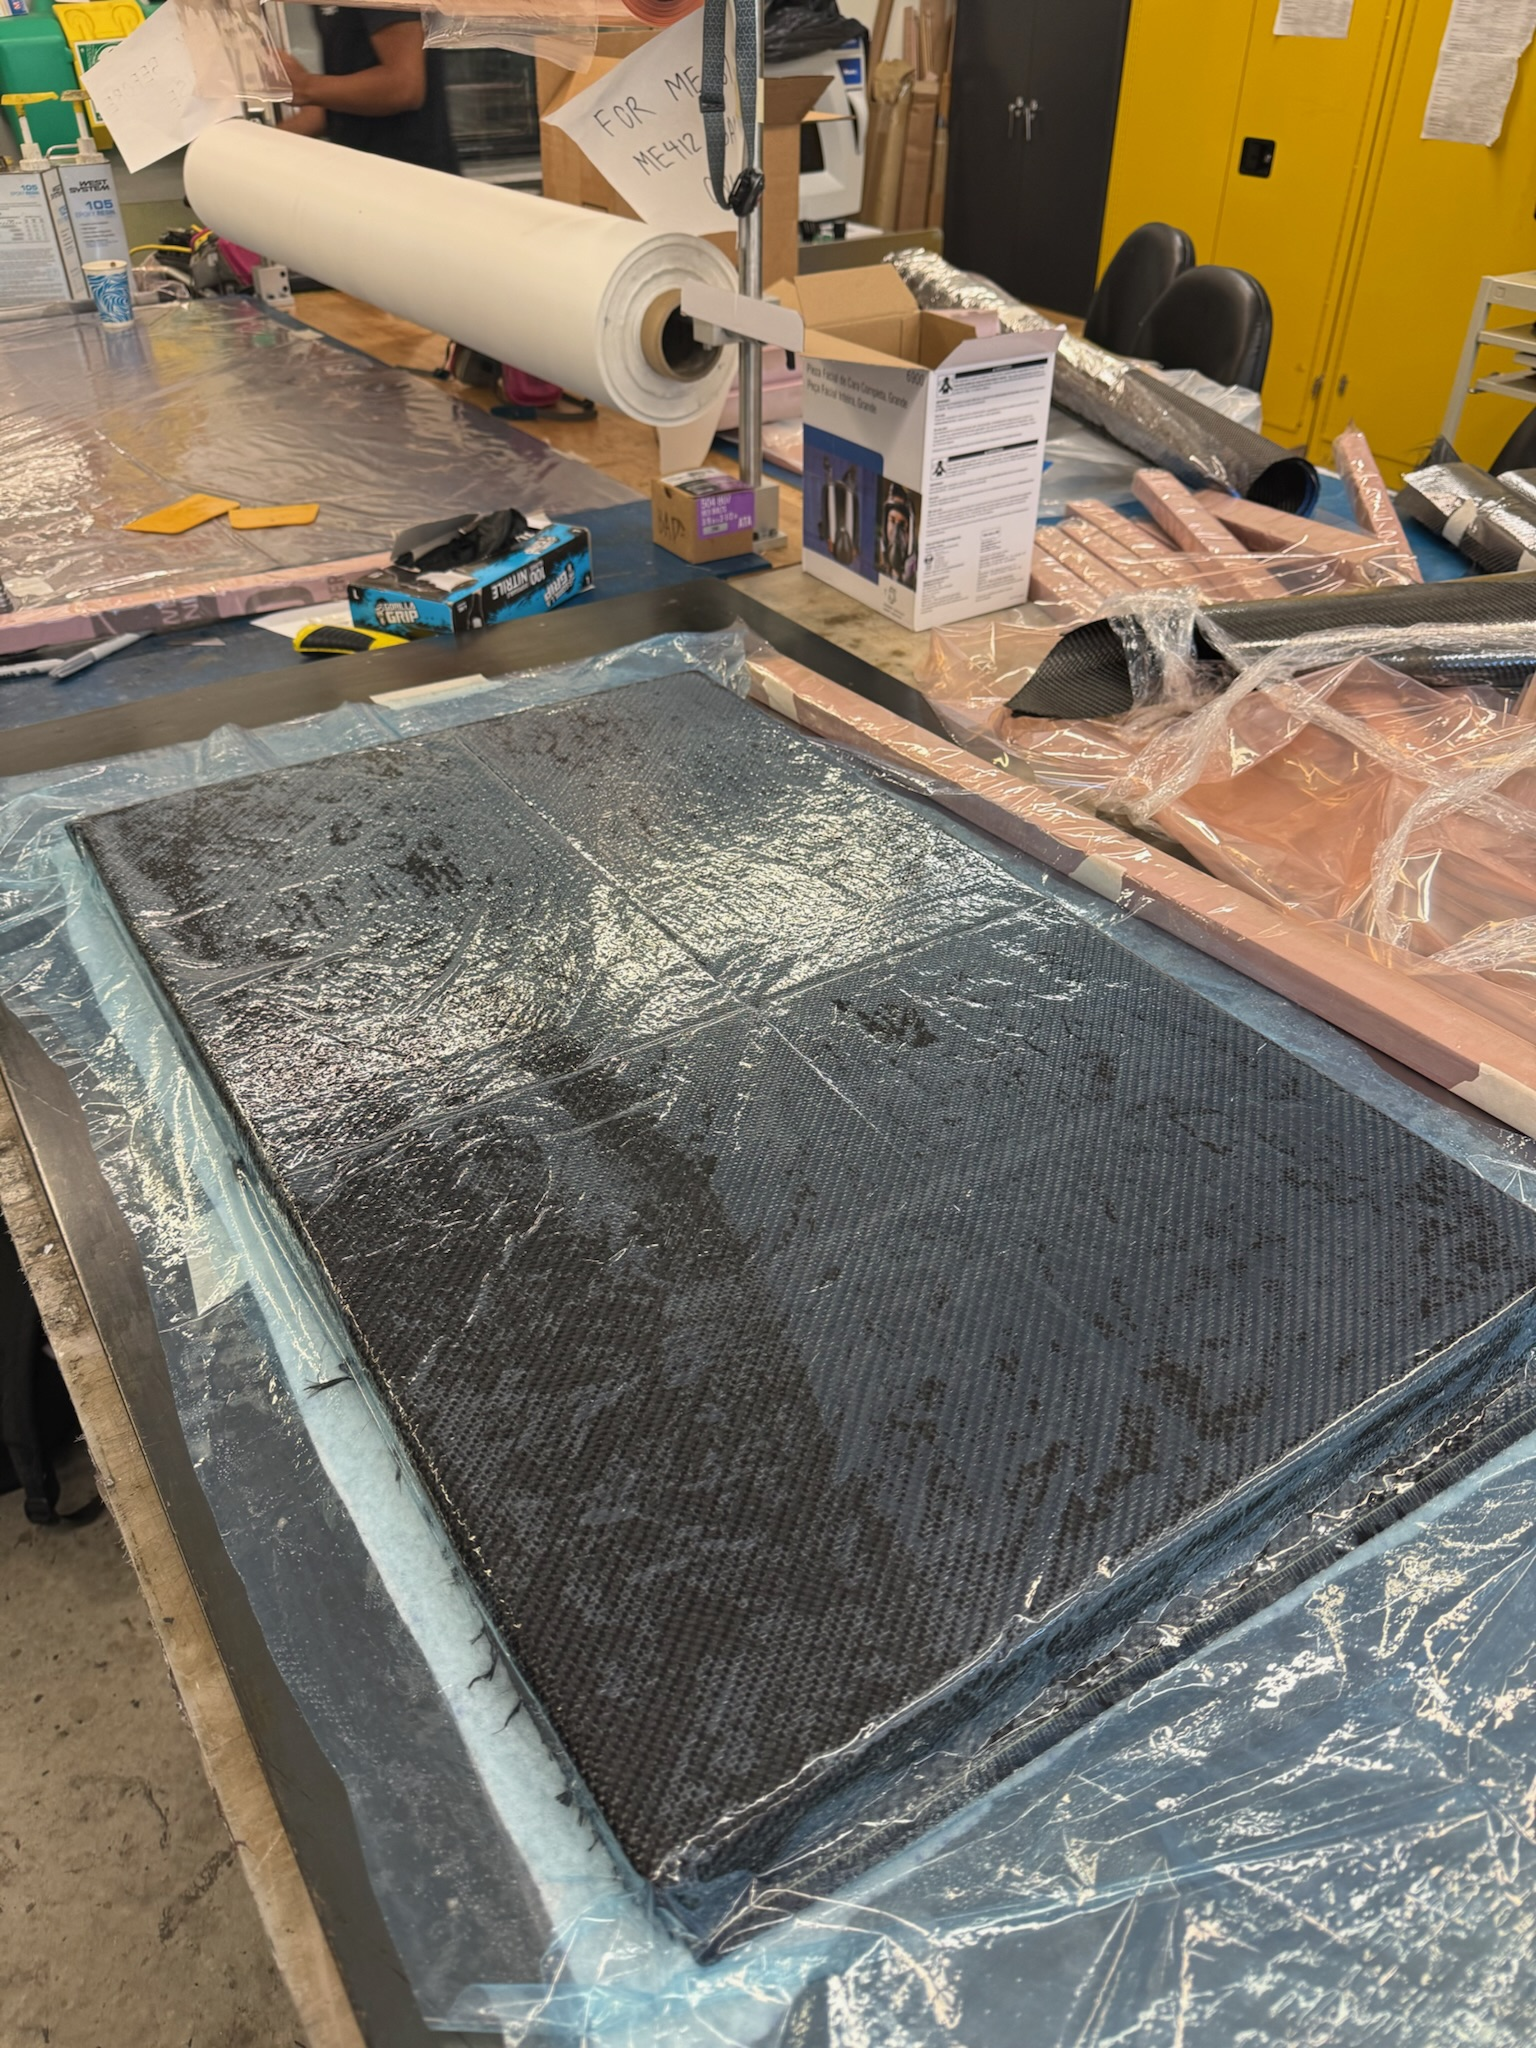
\includegraphics[
        width=3.10in,
        height=1.40in,
        keepaspectratio
    ]{blue_perforrated_film_layup}
};
\draw[RuleGray,line width=0.55pt,rounded corners=4pt]
    ($(current page.north west)+(7.29in,-3.36in)$)
    rectangle
    ($(current page.north east)+(-0.42in,-4.85in)$);

% Row 1 captions
\node[anchor=north,text=Muted,font=\sffamily\fontsize{6.7}{7.3}\selectfont]
at ($(current page.north west)+(2.07in,-4.90in)$)
{1. Waterjet-cut core and perimeter geometry};

\node[anchor=north,text=Muted,font=\sffamily\fontsize{6.7}{7.3}\selectfont]
at ($(current page.north west)+(5.50in,-4.90in)$)
{2. Team wet layup under my process guidance};

\node[anchor=north,text=Muted,font=\sffamily\fontsize{6.7}{7.3}\selectfont]
at ($(current page.north west)+(8.935in,-4.90in)$)
{3. Perforated film, breather, and vacuum enclosure};

% Row 2 image 1
\node[anchor=center,inner sep=0pt]
at ($(current page.north west)+(2.07in,-5.875in)$)
{
    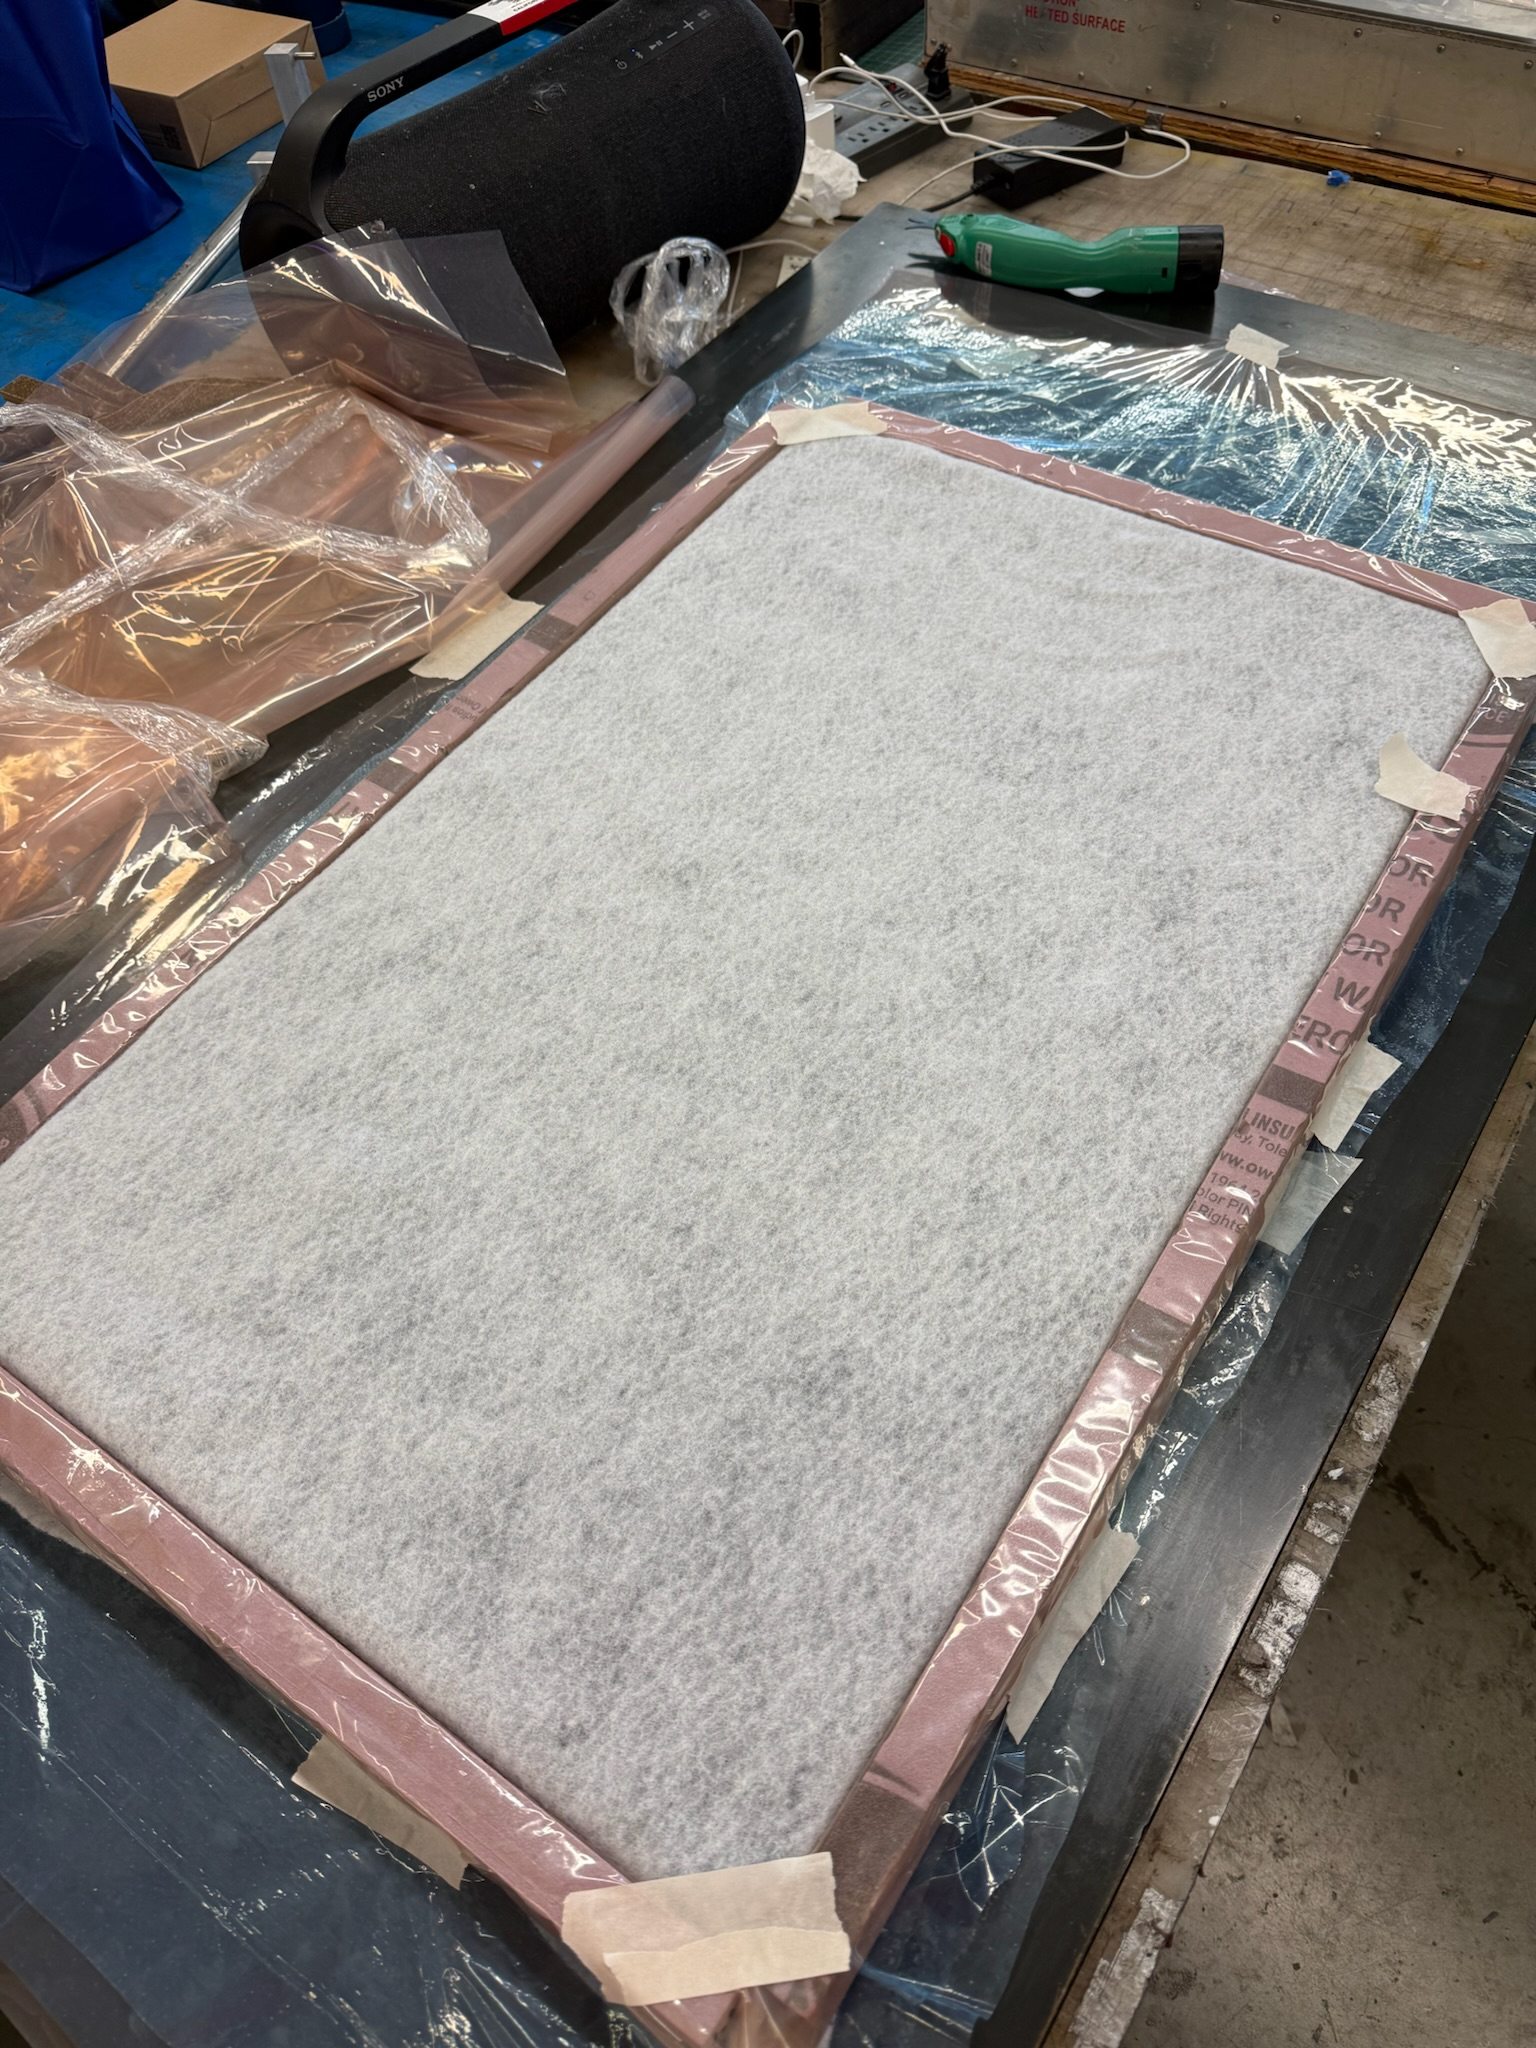
\includegraphics[
        width=3.10in,
        height=1.40in,
        keepaspectratio
    ]{completed_layup}
};
\draw[RuleGray,line width=0.55pt,rounded corners=4pt]
    ($(current page.north west)+(0.43in,-5.13in)$)
    rectangle
    ($(current page.north west)+(3.71in,-6.62in)$);

% Row 2 image 2 — oven chamber used only as a reliable vacuum enclosure; no heat applied
\node[anchor=center,inner sep=0pt]
at ($(current page.north west)+(5.50in,-5.875in)$)
{
    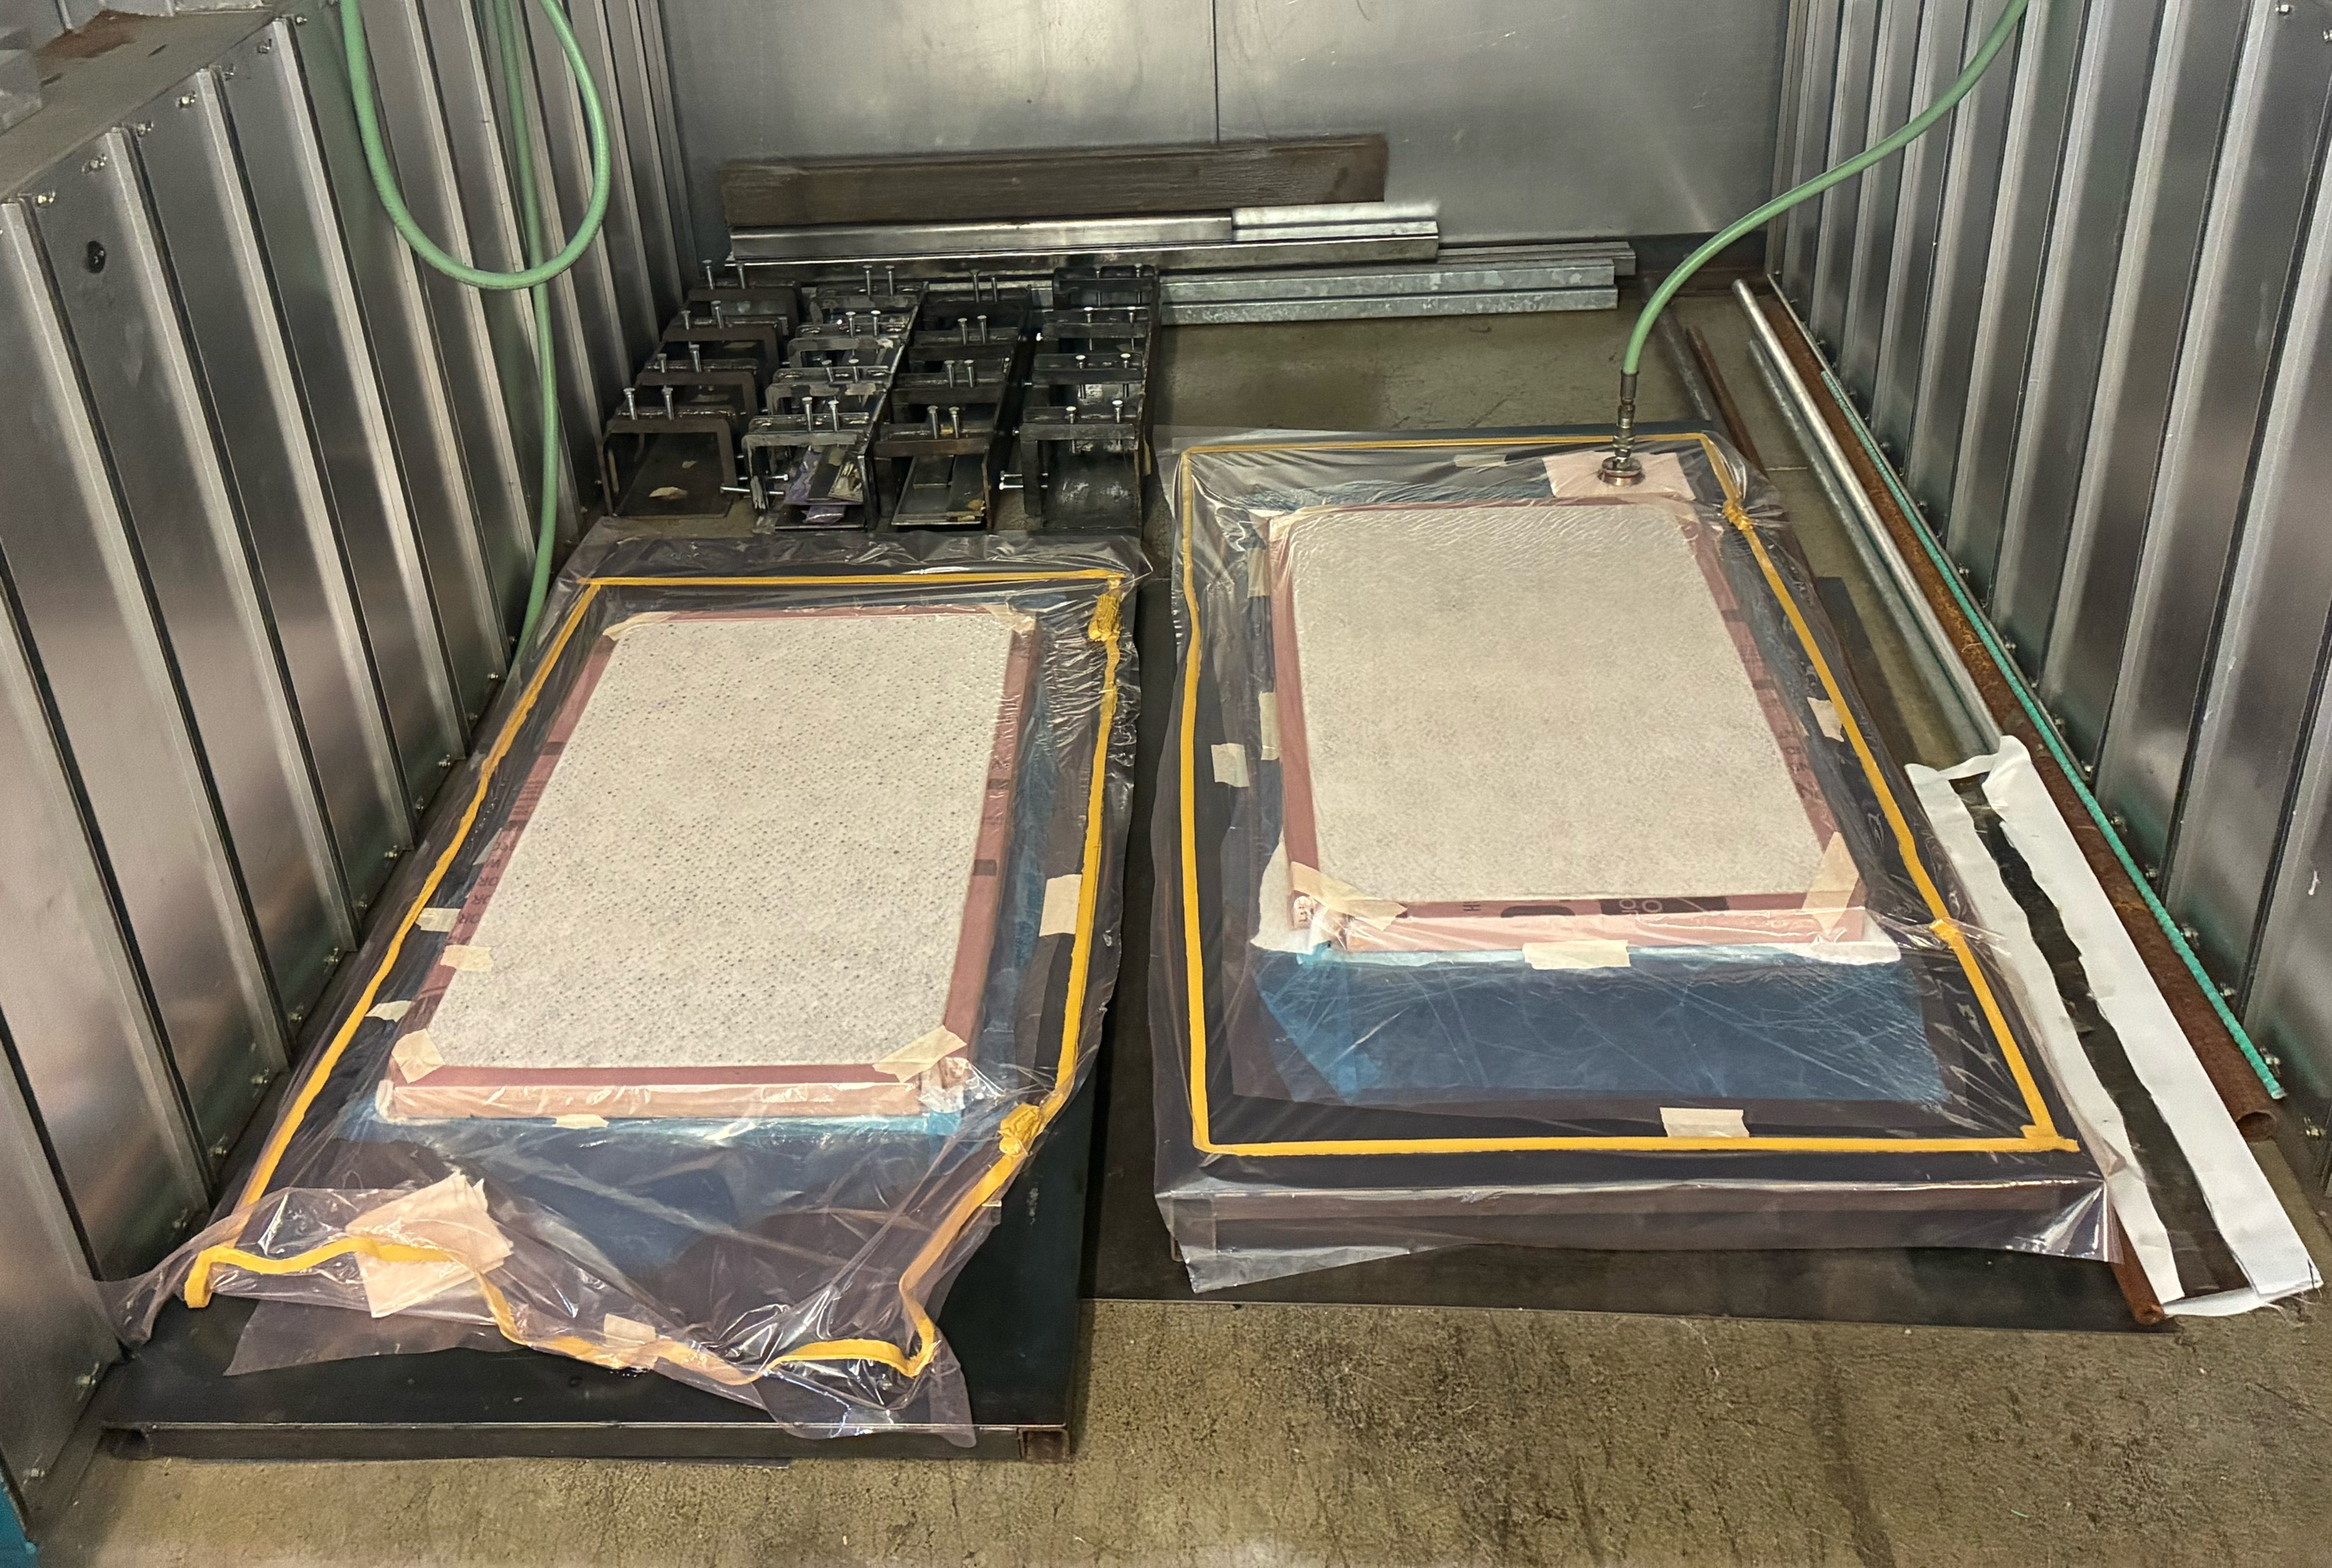
\includegraphics[
        width=3.10in,
        height=1.40in,
        keepaspectratio
    ]{layups_in_composite_oven_under_vacuumPressure}
};
\draw[RuleGray,line width=0.55pt,rounded corners=4pt]
    ($(current page.north west)+(3.86in,-5.13in)$)
    rectangle
    ($(current page.north west)+(7.14in,-6.62in)$);

% Row 2 image 3
\node[anchor=center,inner sep=0pt]
at ($(current page.north west)+(8.935in,-5.875in)$)
{
    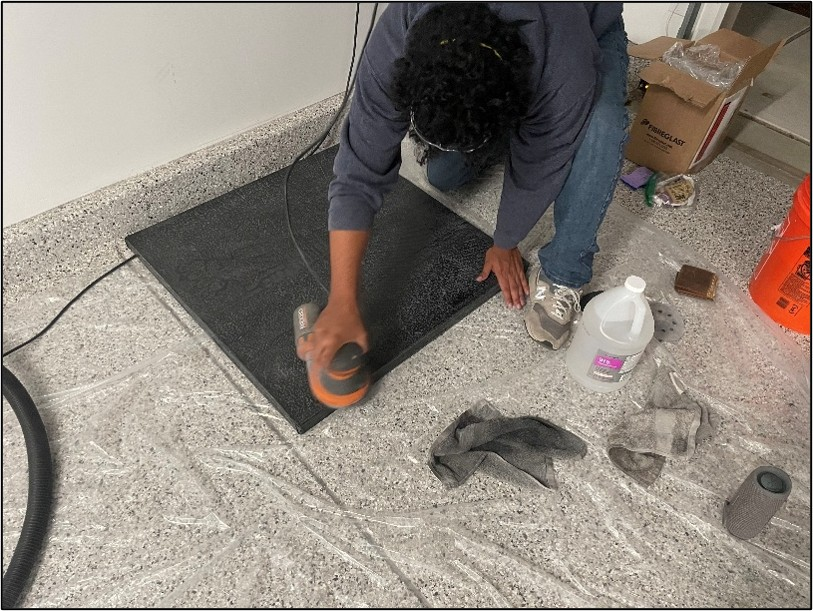
\includegraphics[
        width=3.10in,
        height=1.40in,
        keepaspectratio
    ]{garage_sanding}
};
\draw[RuleGray,line width=0.55pt,rounded corners=4pt]
    ($(current page.north west)+(7.29in,-5.13in)$)
    rectangle
    ($(current page.north east)+(-0.42in,-6.62in)$);

% Row 2 captions
\node[anchor=north,text=Muted,font=\sffamily\fontsize{6.7}{7.3}\selectfont]
at ($(current page.north west)+(2.07in,-6.67in)$)
{4. Fully saturated carbon skin and foam sandwich};

\node[anchor=north,text=Muted,font=\sffamily\fontsize{6.7}{7.3}\selectfont]
at ($(current page.north west)+(5.50in,-6.67in)$)
{5. Room-temperature cure under continuous vacuum};

\node[anchor=north,text=Muted,font=\sffamily\fontsize{6.7}{7.3}\selectfont]
at ($(current page.north west)+(8.935in,-6.67in)$)
{6. Post-processing and surface preparation};

% Bottom callouts
\fill[Panel,rounded corners=4pt]
    ($(current page.north west)+(0.43in,-6.95in)$)
    rectangle
    ($(current page.north west)+(5.48in,-7.60in)$);

\draw[RuleGray,line width=0.55pt,rounded corners=4pt]
    ($(current page.north west)+(0.43in,-6.95in)$)
    rectangle
    ($(current page.north west)+(5.48in,-7.60in)$);

\node[
    anchor=north west,
    text=DeepGreen,
    font=\sffamily\bfseries\fontsize{7.0}{7.6}\selectfont
]
at ($(current page.north west)+(0.63in,-7.08in)$)
{FROM THREE LAYUPS TO ONE};

\node[
    anchor=north west,
    align=left,
    text width=4.56in,
    text=Ink,
    font=\fontsize{6.45}{7.45}\selectfont
]
at ($(current page.north west)+(0.63in,-7.29in)$)
{
The Envelope Method reduced labor, cure cycles, handling,
alignment risk, and time spent forming numerous vacuum-bag
pleats around the 1.5-inch-thick XPS panels.
};

\fill[Panel,rounded corners=4pt]
    ($(current page.north west)+(5.68in,-6.95in)$)
    rectangle
    ($(current page.north east)+(-0.42in,-7.60in)$);

\draw[RuleGray,line width=0.55pt,rounded corners=4pt]
    ($(current page.north west)+(5.68in,-6.95in)$)
    rectangle
    ($(current page.north east)+(-0.42in,-7.60in)$);

\node[
    anchor=north west,
    text=DeepGreen,
    font=\sffamily\bfseries\fontsize{7.0}{7.6}\selectfont
]
at ($(current page.north west)+(5.88in,-7.08in)$)
{WHY SURFACE-BONDED HARDWARE};

\node[
    anchor=north west,
    align=left,
    text width=4.55in,
    text=Ink,
    font=\fontsize{6.45}{7.45}\selectfont
]
at ($(current page.north west)+(5.88in,-7.29in)$)
{
Adhesively bonded hinges and fixtures preserved the clean
composite exterior and avoided drilled inserts, foam-core
crushing, added stress concentrations, and new leak paths.
};


% Footer
\node[
    anchor=south west,
    text=white,
    font=\sffamily\bfseries\fontsize{7.1}{7.7}\selectfont
]
at ($(current page.south west)+(0.42in,0.17in)$)
{\faArrowLeft\ PRODUCT ARCHITECTURE};

\node[
    anchor=south,
    text=white,
    font=\sffamily\fontsize{7.0}{7.6}\selectfont
]
at ($(current page.south)+(0,0.17in)$)
{TORO COVER \hspace{6pt} 2 / 3};

\node[
    anchor=south east,
    text=white,
    font=\sffamily\bfseries\fontsize{7.1}{7.7}\selectfont
]
at ($(current page.south east)+(-0.42in,0.17in)$)
{VALIDATION \& TAKEAWAYS \faArrowRight};

\end{tikzpicture}


% ============================================================
% PAGE 3 — FINISHING, VALIDATION, AND TAKEAWAYS
% ============================================================

\clearpage
\thispagestyle{empty}
\hypertarget{toro-results}{}
\null

\begin{tikzpicture}[remember picture,overlay]

% Background and bars
\fill[white]
    (current page.south west)
    rectangle
    (current page.north east);

\fill[DeepGreen]
    (current page.north west)
    rectangle
    ($(current page.north east)+(0,-0.095in)$);

\fill[PolyGold]
    ($(current page.north west)+(0,-0.095in)$)
    rectangle
    ($(current page.north east)+(0,-0.14in)$);

\fill[DeepGreen]
    (current page.south west)
    rectangle
    ($(current page.south east)+(0,0.36in)$);

\fill[PolyGold]
    ($(current page.south west)+(0,0.36in)$)
    rectangle
    ($(current page.south east)+(0,0.405in)$);

% Header
\node[
    anchor=north west,
    text=PolyGold,
    font=\sffamily\bfseries\fontsize{8.1}{8.7}\selectfont
]
at ($(current page.north west)+(0.42in,-0.39in)$)
{TORO COVER \hspace{5pt}/\hspace{5pt} VALIDATION AND ENGINEERING TAKEAWAYS};

\node[
    anchor=north west,
    text=DeepGreen,
    font=\bfseries\fontsize{22.5}{23.5}\selectfont
]
at ($(current page.north west)+(0.40in,-0.67in)$)
{FROM PROTOTYPE TO PRODUCT PATHWAY};

\node[
    anchor=north west,
    text=Muted,
    font=\sffamily\fontsize{8.7}{9.6}\selectfont
]
at ($(current page.north west)+(0.42in,-1.12in)$)
{Environmental protection, usability testing, scope decisions, and lessons from technical leadership};

\fill[PolyGold]
    ($(current page.north west)+(0.42in,-1.36in)$)
    rectangle
    ($(current page.north west)+(5.8in,-1.315in)$);

% Finishing title
\node[
    anchor=north west,
    text=DeepGreen,
    font=\sffamily\bfseries\fontsize{8.0}{8.7}\selectfont
]
at ($(current page.north west)+(0.43in,-1.62in)$)
{OUTDOOR FINISHING AND ENVIRONMENTAL PROTECTION};

% Image 1
\node[anchor=center,inner sep=0pt]
at ($(current page.north west)+(1.705in,-2.655in)$)
{
    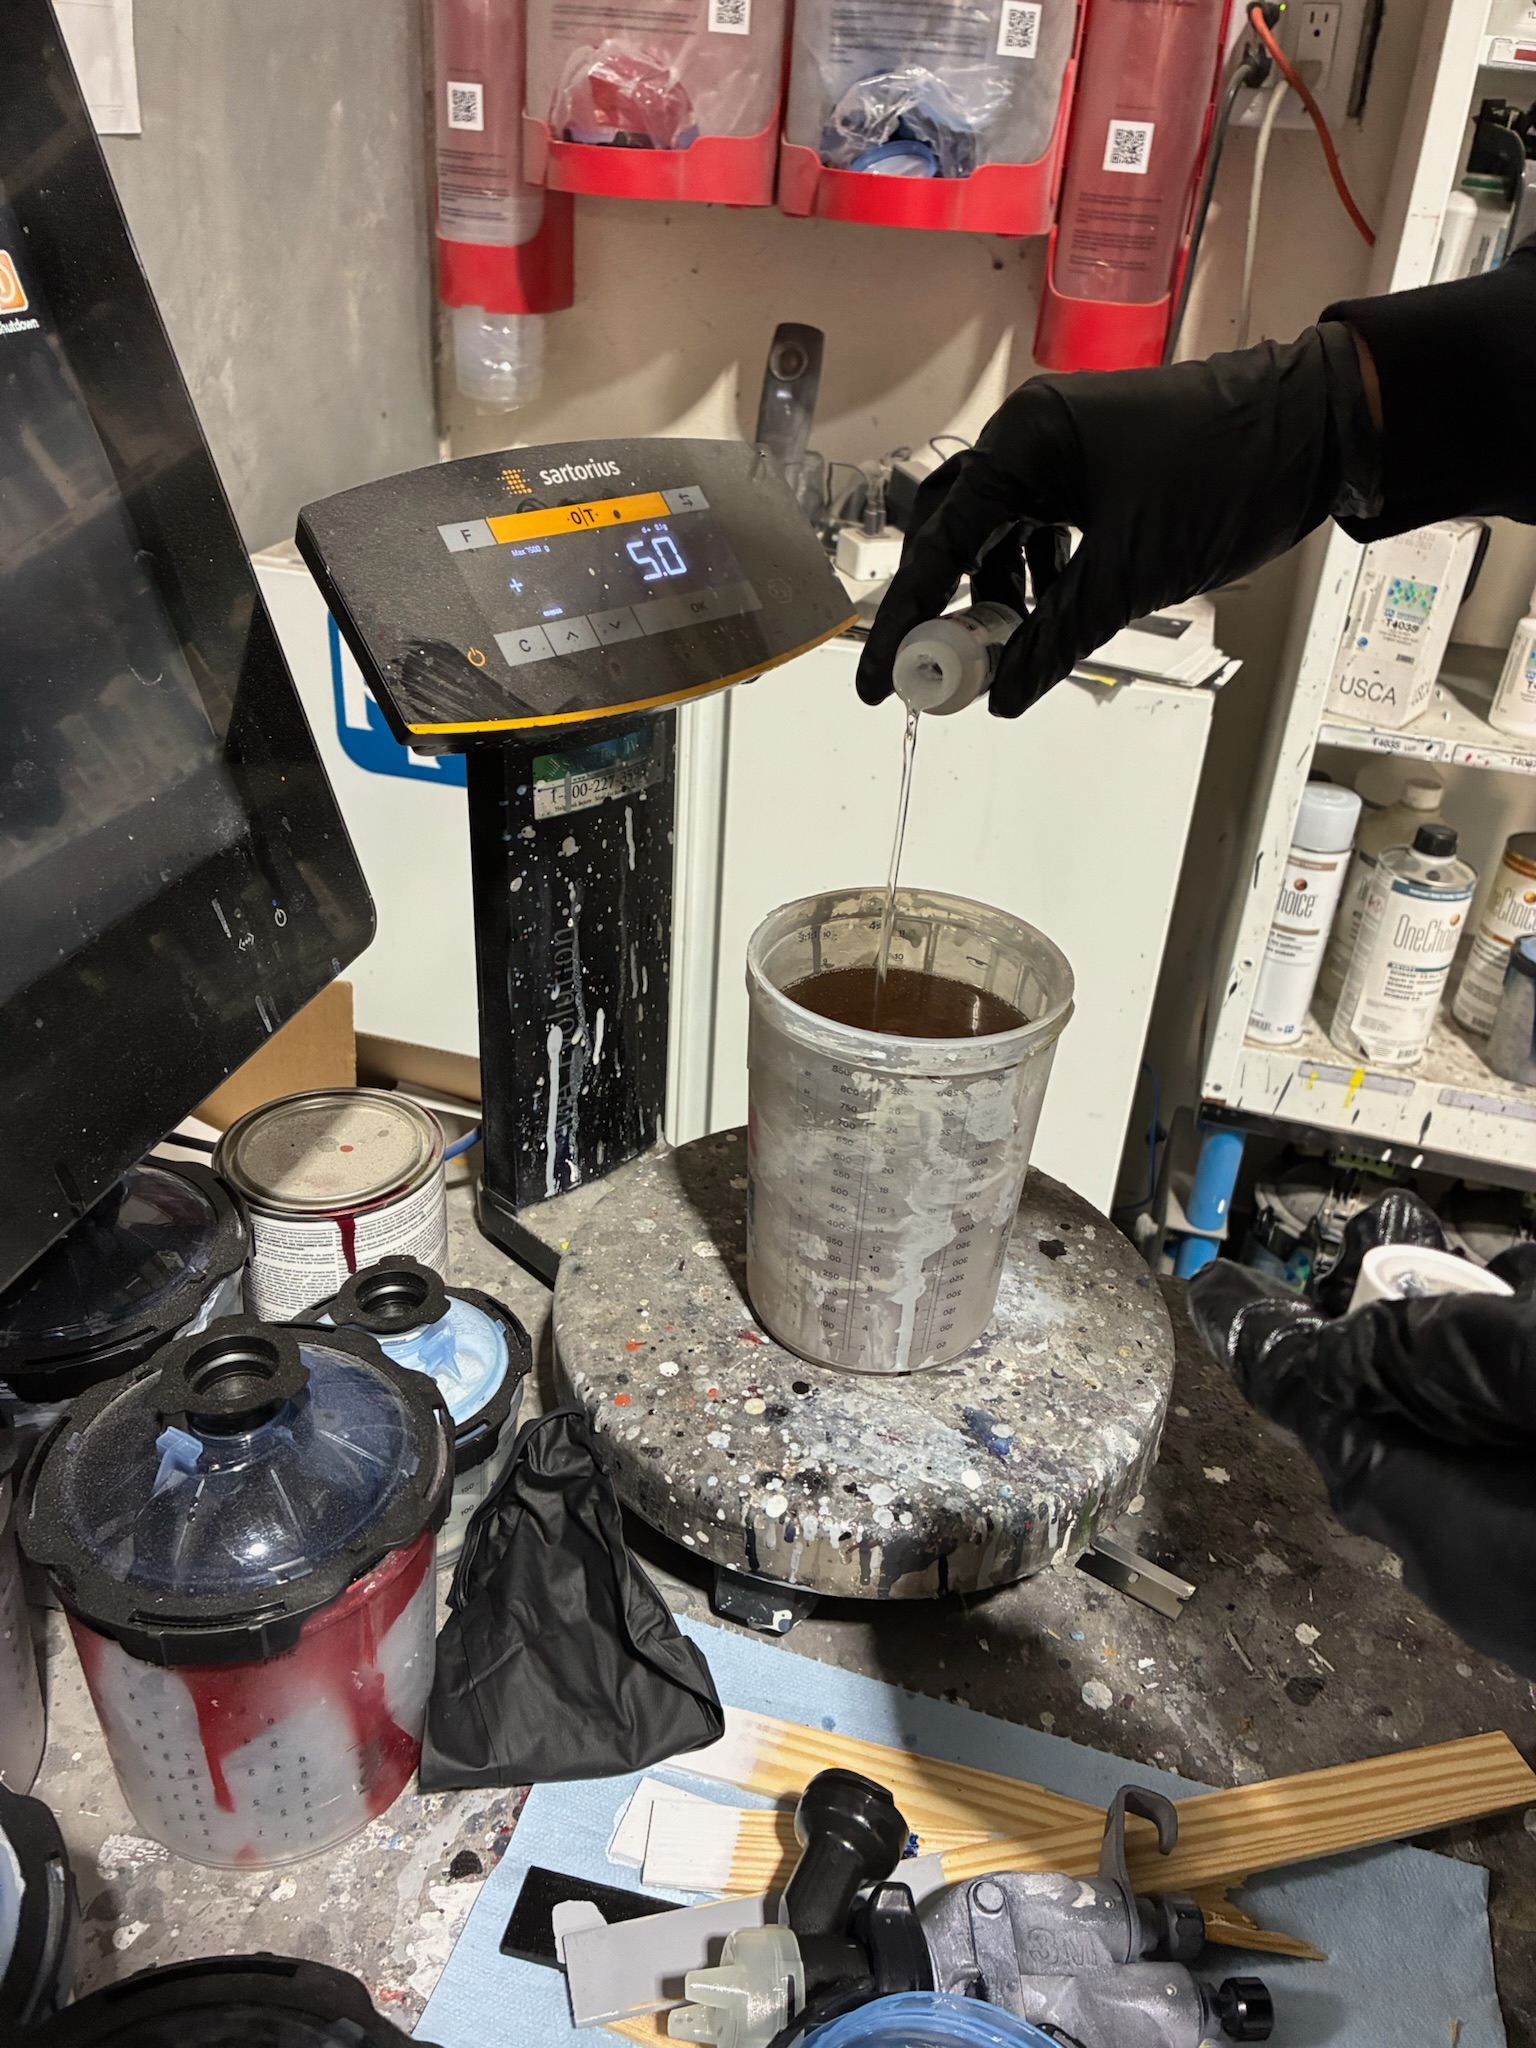
\includegraphics[
        width=2.35in,
        height=1.40in,
        keepaspectratio
    ]{spray_topcoat_prep}
};
\draw[RuleGray,line width=0.55pt,rounded corners=4pt]
    ($(current page.north west)+(0.43in,-1.91in)$)
    rectangle
    ($(current page.north west)+(2.98in,-3.40in)$);

% Image 2
\node[anchor=center,inner sep=0pt]
at ($(current page.north west)+(4.375in,-2.655in)$)
{
    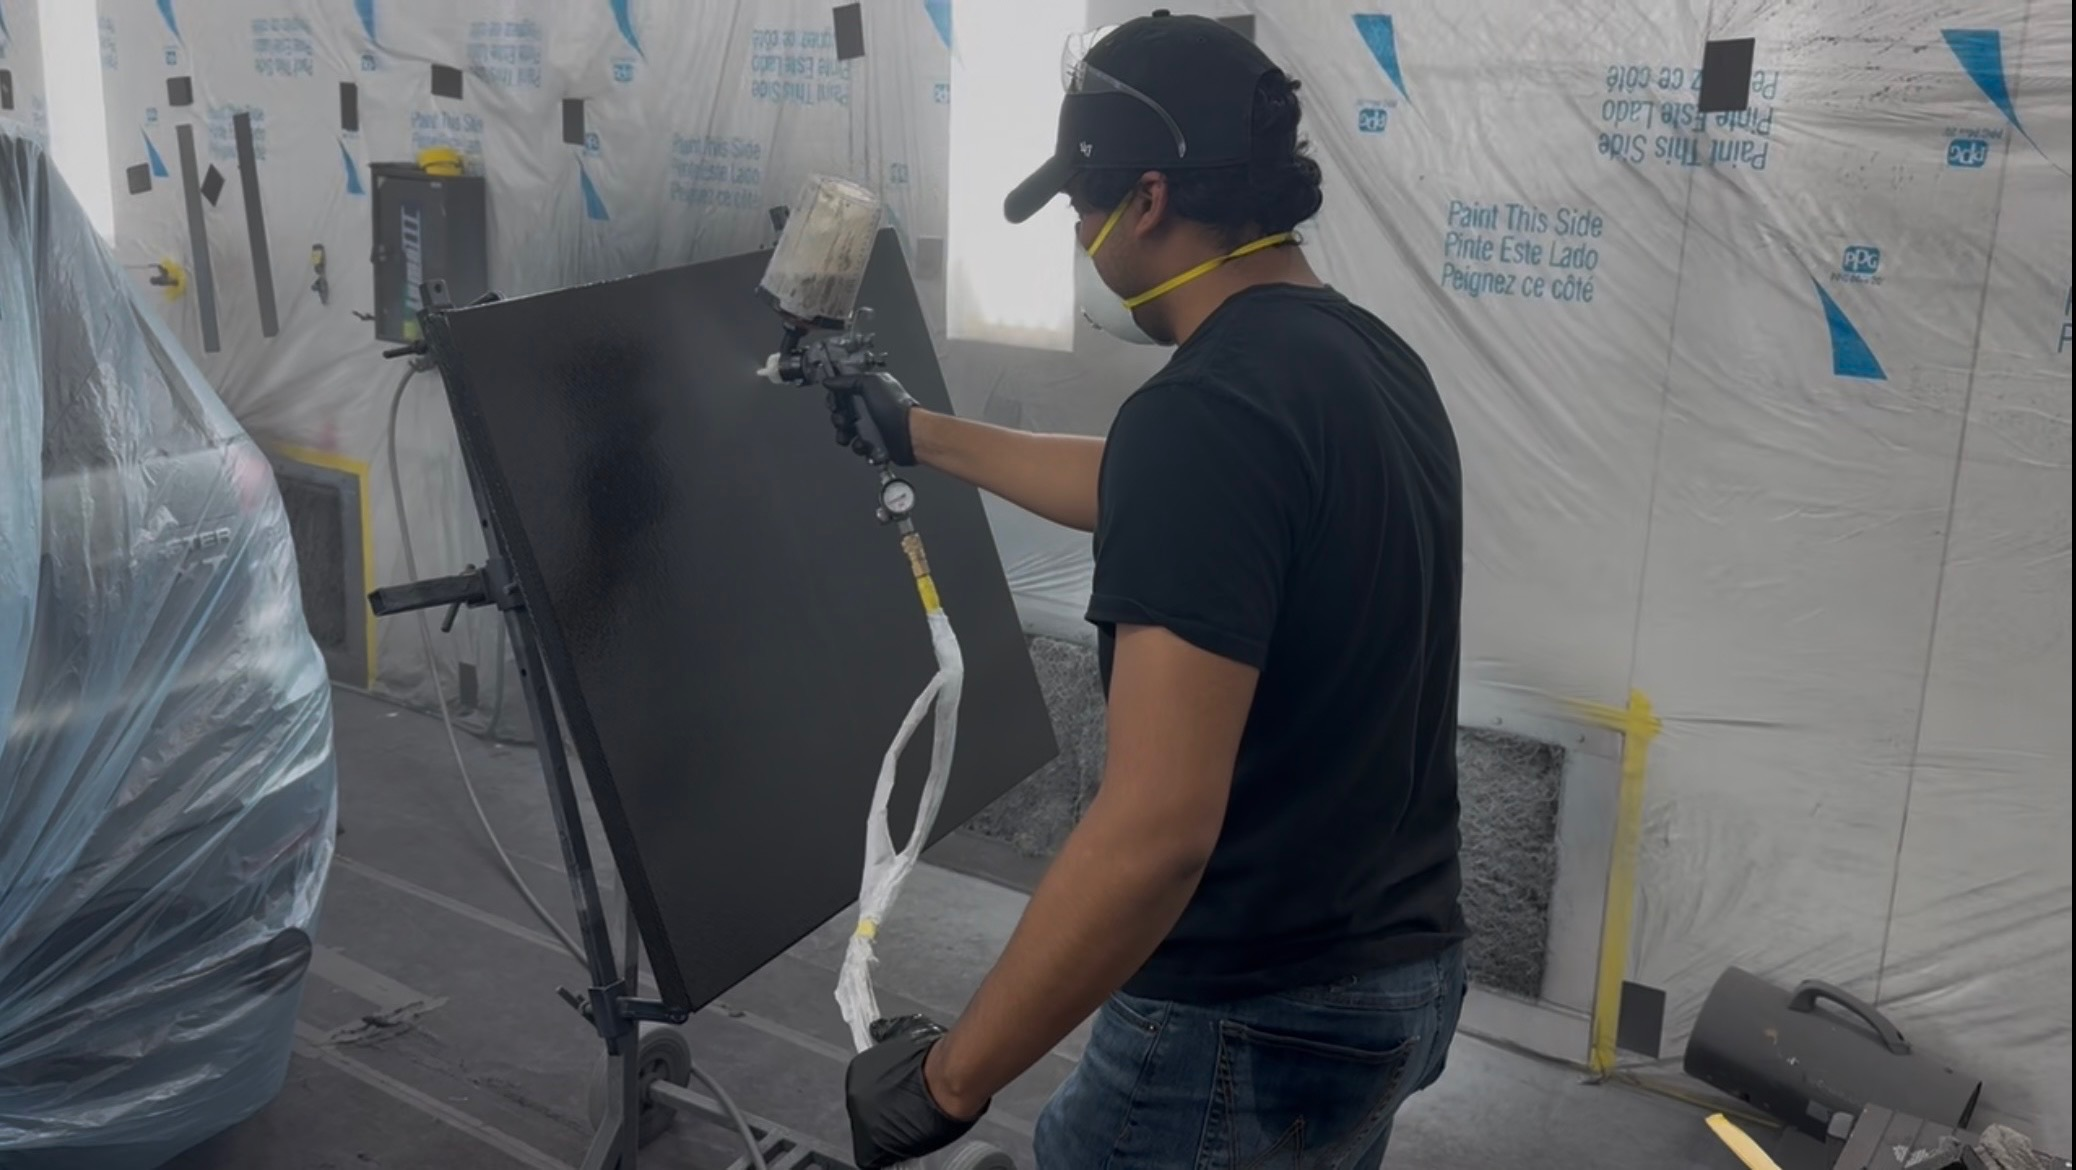
\includegraphics[
        width=2.35in,
        height=1.40in,
        keepaspectratio
    ]{spraying_topcoat}
};
\draw[RuleGray,line width=0.55pt,rounded corners=4pt]
    ($(current page.north west)+(3.10in,-1.91in)$)
    rectangle
    ($(current page.north west)+(5.65in,-3.40in)$);

% Image 3
\node[anchor=center,inner sep=0pt]
at ($(current page.north west)+(7.045in,-2.655in)$)
{
    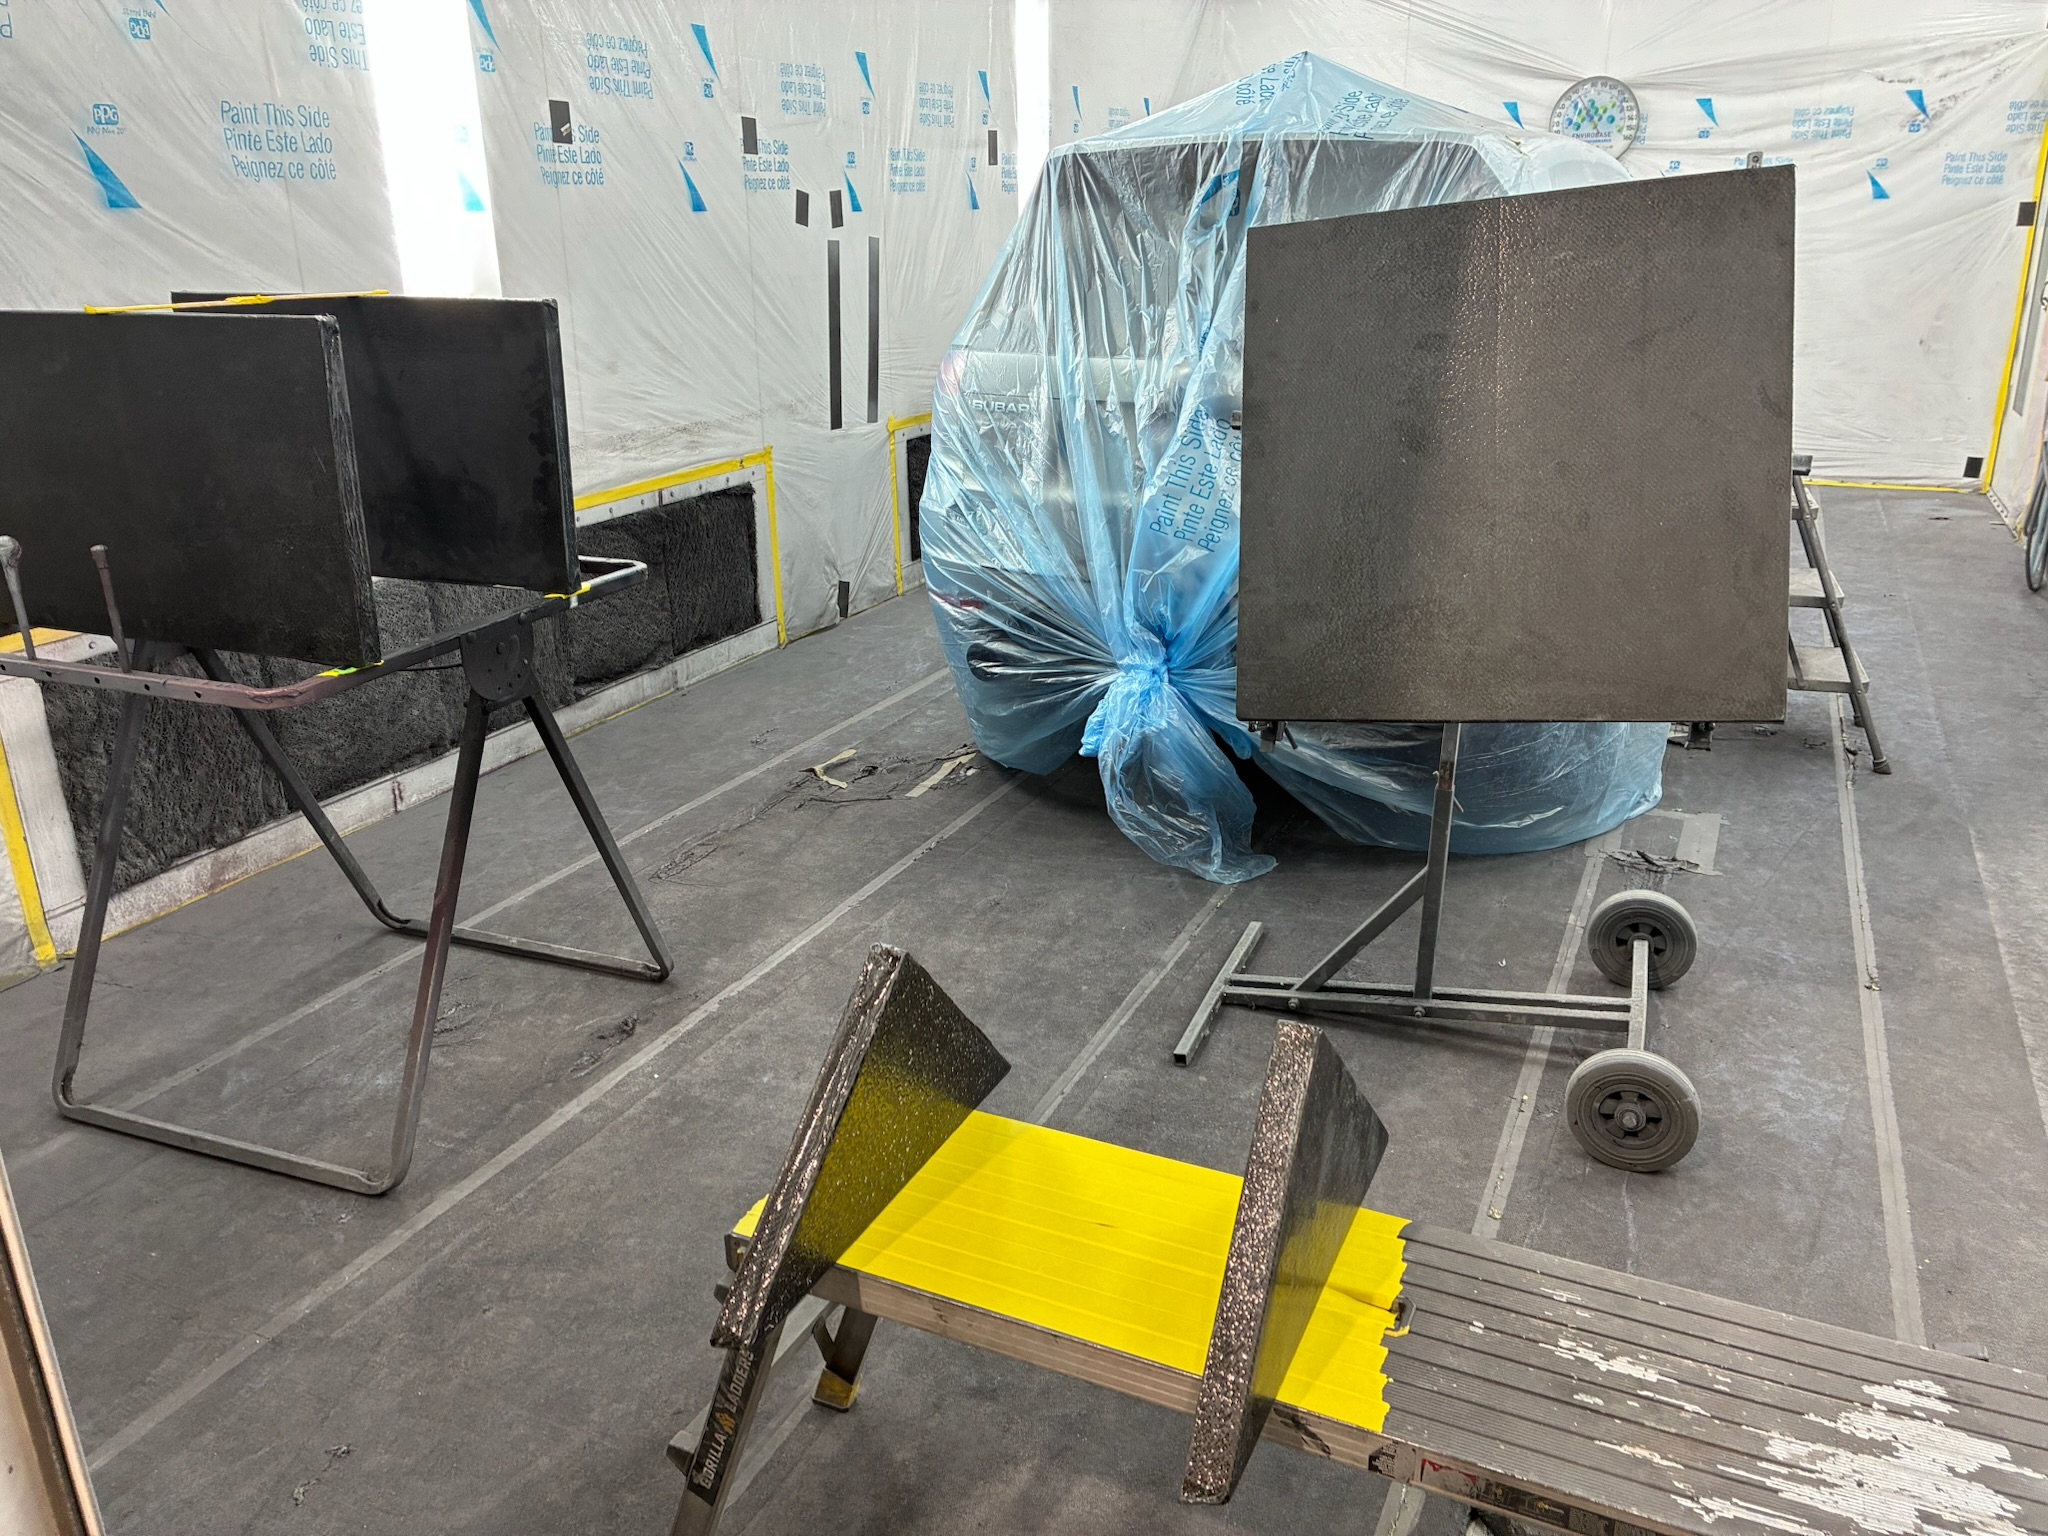
\includegraphics[
        width=2.35in,
        height=1.40in,
        keepaspectratio
    ]{topcoat_setup_apparatus}
};
\draw[RuleGray,line width=0.55pt,rounded corners=4pt]
    ($(current page.north west)+(5.77in,-1.91in)$)
    rectangle
    ($(current page.north west)+(8.32in,-3.40in)$);

% Image 4
\node[anchor=center,inner sep=0pt]
at ($(current page.north west)+(9.50in,-2.655in)$)
{
    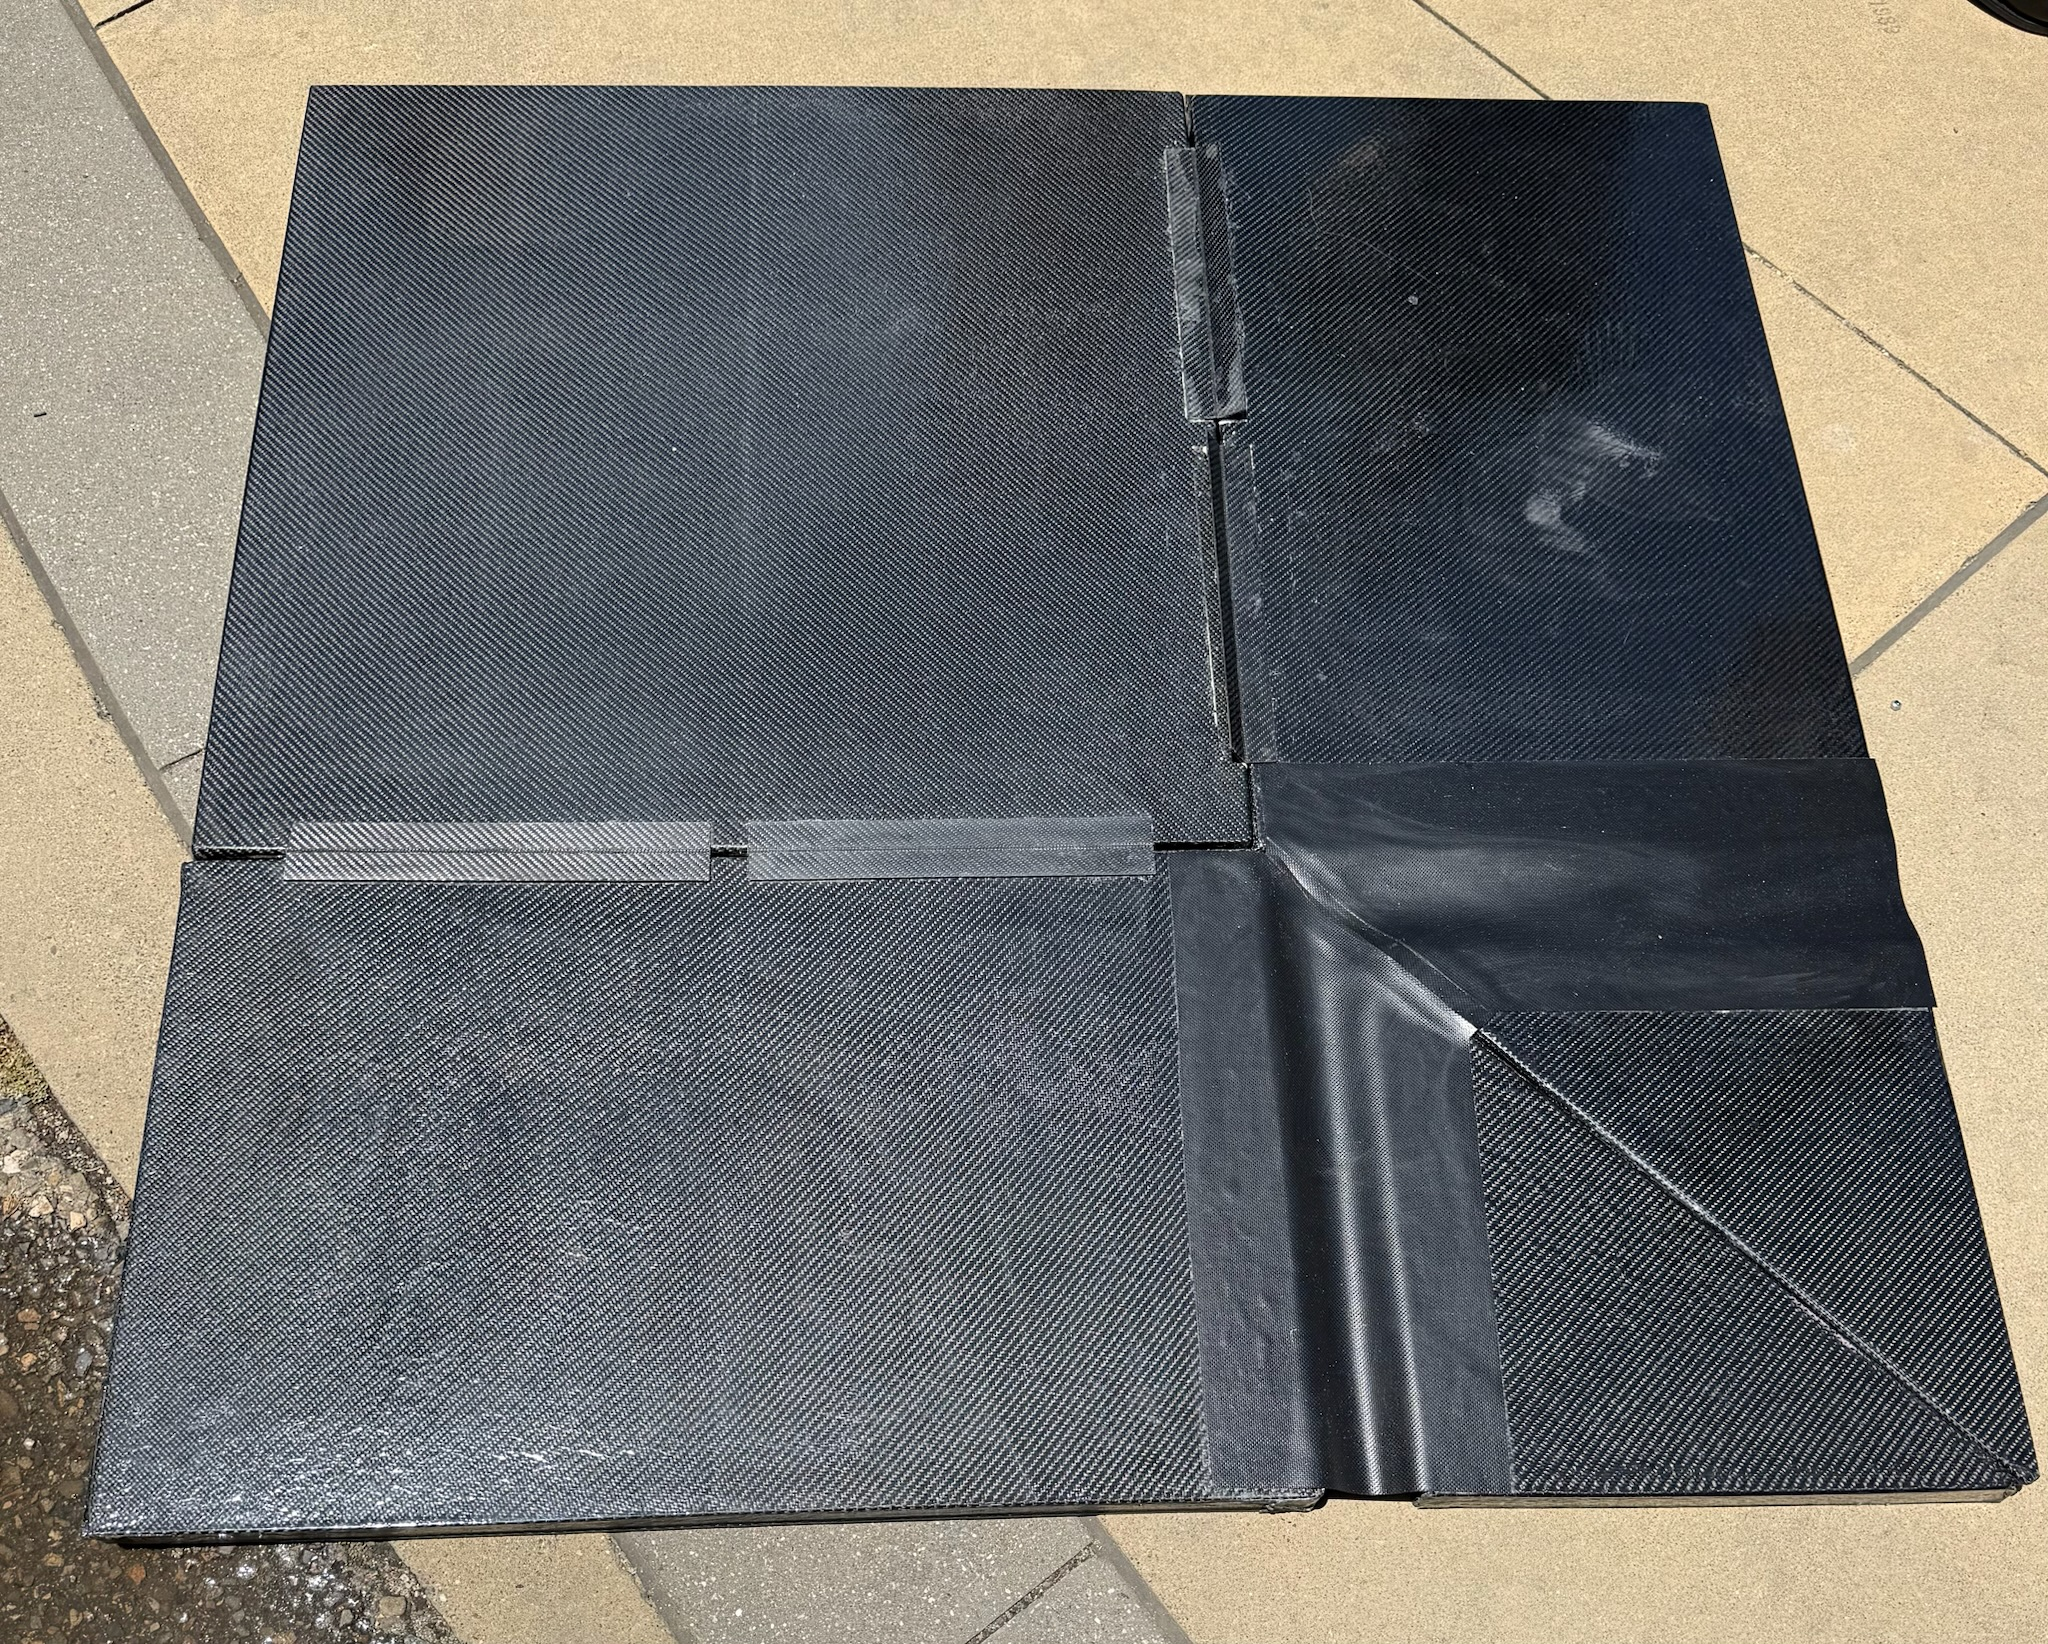
\includegraphics[
        width=2.35in,
        height=1.40in,
        keepaspectratio
    ]{refined_final_toro_cover_partial_carbon_model}
};
\draw[RuleGray,line width=0.55pt,rounded corners=4pt]
    ($(current page.north west)+(8.44in,-1.91in)$)
    rectangle
    ($(current page.north east)+(-0.42in,-3.40in)$);

% Captions
\node[anchor=north,text=Muted,font=\sffamily\fontsize{6.7}{7.3}\selectfont]
at ($(current page.north west)+(1.705in,-3.45in)$)
{Topcoat material preparation};

\node[anchor=north,text=Muted,font=\sffamily\fontsize{6.7}{7.3}\selectfont]
at ($(current page.north west)+(4.375in,-3.45in)$)
{Automotive-booth topcoat application};

\node[anchor=north,text=Muted,font=\sffamily\fontsize{6.7}{7.3}\selectfont]
at ($(current page.north west)+(7.045in,-3.45in)$)
{Coated panels drying after application};

\node[anchor=north,text=Muted,font=\sffamily\fontsize{6.7}{7.3}\selectfont]
at ($(current page.north west)+(9.50in,-3.45in)$)
{Partial carbon manufacturing model};

% Environmental rationale
\fill[SoftGold,rounded corners=4pt]
    ($(current page.north west)+(0.43in,-3.73in)$)
    rectangle
    ($(current page.north east)+(-0.42in,-4.76in)$);

\node[
    anchor=north west,
    align=left,
    text width=9.75in,
    text=Ink,
    font=\fontsize{7.05}{8.25}\selectfont
]
at ($(current page.north west)+(0.65in,-3.89in)$)
{
Because the sponsor required a carbon-fiber cover for outdoor use near chlorinated water,
environmental protection became a functional requirement rather than a cosmetic finish.
I selected and personally sprayed a UV-resistant Sunshield topcoat to seal minor laminate
porosity, reduce moisture ingress, preserve the carbon appearance, limit UV degradation of
the epoxy matrix, and isolate the composite surface from nearby metallic hardware.
};

% Results title
\node[
    anchor=north west,
    text=DeepGreen,
    font=\sffamily\bfseries\fontsize{8.0}{8.7}\selectfont
]
at ($(current page.north west)+(0.43in,-4.94in)$)
{FUNCTIONAL PROTOTYPE RESULTS};

% ------------------------------------------------------------
% Matched lower panels — larger type and improved allocation
% ------------------------------------------------------------

% Left results panel
\fill[SoftGreen,rounded corners=5pt]
    ($(current page.north west)+(0.43in,-5.22in)$)
    rectangle
    ($(current page.north west)+(5.98in,-7.39in)$);

\draw[RuleGray,line width=0.65pt,rounded corners=5pt]
    ($(current page.north west)+(0.43in,-5.22in)$)
    rectangle
    ($(current page.north west)+(5.98in,-7.39in)$);

\fill[DeepGreen,rounded corners=5pt]
    ($(current page.north west)+(0.43in,-5.22in)$)
    rectangle
    ($(current page.north west)+(5.98in,-5.58in)$);

\fill[DeepGreen]
    ($(current page.north west)+(0.43in,-5.40in)$)
    rectangle
    ($(current page.north west)+(5.98in,-5.58in)$);

\node[anchor=west,text=white,
      font=\sffamily\bfseries\fontsize{7.0}{7.6}\selectfont]
at ($(current page.north west)+(0.66in,-5.40in)$)
{SPECIFICATION};

\node[anchor=west,text=white,
      font=\sffamily\bfseries\fontsize{7.0}{7.6}\selectfont]
at ($(current page.north west)+(3.02in,-5.40in)$)
{RESULT};

\node[anchor=east,text=white,
      font=\sffamily\bfseries\fontsize{7.0}{7.6}\selectfont]
at ($(current page.north west)+(5.55in,-5.40in)$)
{STATUS};

\node[
    anchor=north west,
    align=left,
    text width=2.15in,
    text=Ink,
    font=\bfseries\fontsize{7.15}{8.55}\selectfont
]
at ($(current page.north west)+(0.66in,-5.72in)$)
{
Deployment time\\[3.4pt]
Removal time\\[3.4pt]
Single-user operation\\[3.4pt]
Single-side operation\\[3.4pt]
Deployment steps\\[3.4pt]
Removal steps\\[3.4pt]
Weight\\[3.4pt]
Folded storage
};

\node[
    anchor=north west,
    align=left,
    text width=1.45in,
    text=Ink,
    font=\fontsize{7.15}{8.55}\selectfont
]
at ($(current page.north west)+(3.02in,-5.72in)$)
{
25.51 seconds\\[3.4pt]
37.22 seconds\\[3.4pt]
100\% successful\\[3.4pt]
75\% successful\\[3.4pt]
6.4 average\\[3.4pt]
9 average\\[3.4pt]
17 lb\\[3.4pt]
2.9' x 2.9' x 1.7'
};

\node[
    anchor=north east,
    align=right,
    text width=1.05in,
    text=DeepGreen,
    font=\sffamily\bfseries\fontsize{7.05}{8.55}\selectfont
]
at ($(current page.north west)+(5.55in,-5.72in)$)
{
PASS\\[3.4pt]
PASS\\[3.4pt]
PASS\\[3.4pt]
NEAR TARGET\\[3.4pt]
PASS\\[3.4pt]
PASS\\[3.4pt]
NEAR TARGET\\[3.4pt]
PASS
};

% Right takeaways panel — widened for easier reading
\fill[SoftGreen,rounded corners=5pt]
    ($(current page.north west)+(6.14in,-5.22in)$)
    rectangle
    ($(current page.north east)+(-0.42in,-7.39in)$);

\draw[RuleGray,line width=0.65pt,rounded corners=5pt]
    ($(current page.north west)+(6.14in,-5.22in)$)
    rectangle
    ($(current page.north east)+(-0.42in,-7.39in)$);

\fill[DeepGreen,rounded corners=5pt]
    ($(current page.north west)+(6.14in,-5.22in)$)
    rectangle
    ($(current page.north east)+(-0.42in,-5.58in)$);

\fill[DeepGreen]
    ($(current page.north west)+(6.14in,-5.40in)$)
    rectangle
    ($(current page.north east)+(-0.42in,-5.58in)$);

\node[anchor=west,text=white,
      font=\sffamily\bfseries\fontsize{7.1}{7.7}\selectfont]
at ($(current page.north west)+(6.38in,-5.40in)$)
{ENGINEERING TAKEAWAYS};

\node[
    anchor=north west,
    align=left,
    text width=4.02in,
    text=Ink,
    font=\fontsize{6.75}{7.85}\selectfont
]
at ($(current page.north west)+(6.38in,-5.72in)$)
{
\textbf{Manufacturing first.}
Composite manufacturing constraints should guide the product architecture from the beginning.\\[4.5pt]
\textbf{Prioritize deliberately.}
Competing requirements must be balanced intentionally instead of maximizing every objective.\\[4.5pt]
\textbf{Lead through the process.}
Clear procedures, calm communication, and respect for teammates' strengths were essential during fabrication.\\[4.5pt]
\textbf{Next iteration.}
Reduce weight, refine the fabric-hinge fold lines, and improve panel-edge clearance.
};

% Compact concluding pathway
\node[
    anchor=center,
    align=center,
    text=PolyGold,
    font=\sffamily\bfseries\fontsize{6.3}{6.9}\selectfont
]
at ($(current page.north)+(3.06in,-7.18in)$)
{PROTOTYPE \faArrowRight\ DESIGN REFINEMENT
\faArrowRight\ REPEATABLE MANUFACTURING
\faArrowRight\ PRODUCT};

% Validation resources
\node[
    anchor=north,
    align=center,
    text=DeepGreen,
    font=\sffamily\bfseries\fontsize{6.6}{7.2}\selectfont
]
at ($(current page.north)+(0,-7.58in)$)
{\href{\ToroDeploymentLink}{\faPlayCircle\ DEPLOYMENT}
\hspace{18pt}
\href{\ToroRemovalLink}{\faPlayCircle\ REMOVAL / FOLDING}
\hspace{18pt}
\href{\ToroPosterLink}{\faFilePdf\ EXPO POSTER}
\hspace{18pt}
\href{\ToroReportLink}{\faFilePdf\ FINAL REPORT}};

% Footer
\node[
    anchor=south west,
    text=white,
    font=\sffamily\bfseries\fontsize{7.1}{7.7}\selectfont
]
at ($(current page.south west)+(0.42in,0.17in)$)
{\faArrowLeft\ MANUFACTURING-DRIVEN DESIGN};

\node[
    anchor=south,
    text=white,
    font=\sffamily\fontsize{7.0}{7.6}\selectfont
]
at ($(current page.south)+(0,0.17in)$)
{TORO COVER \hspace{6pt} 3 / 3};

\node[
    anchor=south east,
    text=white,
    font=\sffamily\bfseries\fontsize{7.1}{7.7}\selectfont
]
at ($(current page.south east)+(-0.42in,0.17in)$)
{NEXT PROJECT \faArrowRight};

\end{tikzpicture}

% ============================================================
% PICKLEBALL PADDLE — SINGLE-PAGE PORTFOLIO CASE STUDY
% Project 02 in the Composites section
%
% IMPORTANT:
% 1. This file must NOT contain \documentclass, \begin{document},
%    or \end{document}.
% 2. In main.tex, place \input{pickleball} before \end{document}.
% 3. Image references use these Overleaf base filenames:
%       waterjet
%       side_core_view
%       full_assy
%       front_view
%       LAMINATE
% ============================================================

% Clickable project resource
\providecommand{\PaddleWaterjetVideo}
{https://drive.google.com/file/d/1mTuaE_g5mE2f7Nn3R5k7yFxqCWH_pvBh/view?usp=drive_link}

\clearpage
\thispagestyle{empty}
\hypertarget{pickleball}{}
\null

\begin{tikzpicture}[remember picture,overlay]

% ============================================================
% BACKGROUND AND PAGE BARS
% ============================================================

\fill[white]
    (current page.south west)
    rectangle
    (current page.north east);

\fill[DeepGreen]
    (current page.north west)
    rectangle
    ($(current page.north east)+(0,-0.095in)$);

\fill[PolyGold]
    ($(current page.north west)+(0,-0.095in)$)
    rectangle
    ($(current page.north east)+(0,-0.14in)$);

\fill[DeepGreen]
    (current page.south west)
    rectangle
    ($(current page.south east)+(0,0.36in)$);

\fill[PolyGold]
    ($(current page.south west)+(0,0.36in)$)
    rectangle
    ($(current page.south east)+(0,0.405in)$);

% ============================================================
% HEADER
% ============================================================

\node[
    anchor=north west,
    text=PolyGold,
    font=\sffamily\bfseries\fontsize{8.1}{8.7}\selectfont
]
at ($(current page.north west)+(0.42in,-0.39in)$)
{01 COMPOSITES \hspace{5pt}/\hspace{5pt} PROJECT 02};

\node[
    anchor=north west,
    text=DeepGreen,
    font=\bfseries\fontsize{22.5}{23.5}\selectfont
]
at ($(current page.north west)+(0.40in,-0.67in)$)
{CARBON FIBER PICKLEBALL PADDLE};

\node[
    anchor=north west,
    text=Muted,
    font=\sffamily\fontsize{8.4}{9.2}\selectfont
]
at ($(current page.north west)+(0.42in,-1.12in)$)
{Cal Poly Composites Laboratory \hspace{7pt}\textbullet\hspace{7pt}
Individual Project \hspace{7pt}\textbullet\hspace{7pt}
Spring 2026 \hspace{7pt}\textbullet\hspace{7pt}
San Luis Obispo, California};

\fill[PolyGold]
    ($(current page.north west)+(0.42in,-1.36in)$)
    rectangle
    ($(current page.north west)+(6.10in,-1.315in)$);

% ============================================================
% TOP LEFT — HERO PRODUCT IMAGE
% ============================================================

\node[
    anchor=center,
    inner sep=3pt,
    draw=DeepGreen,
    line width=0.75pt,
    rounded corners=6pt
]
at ($(current page.north west)+(1.60in,-3.20in)$)
{
    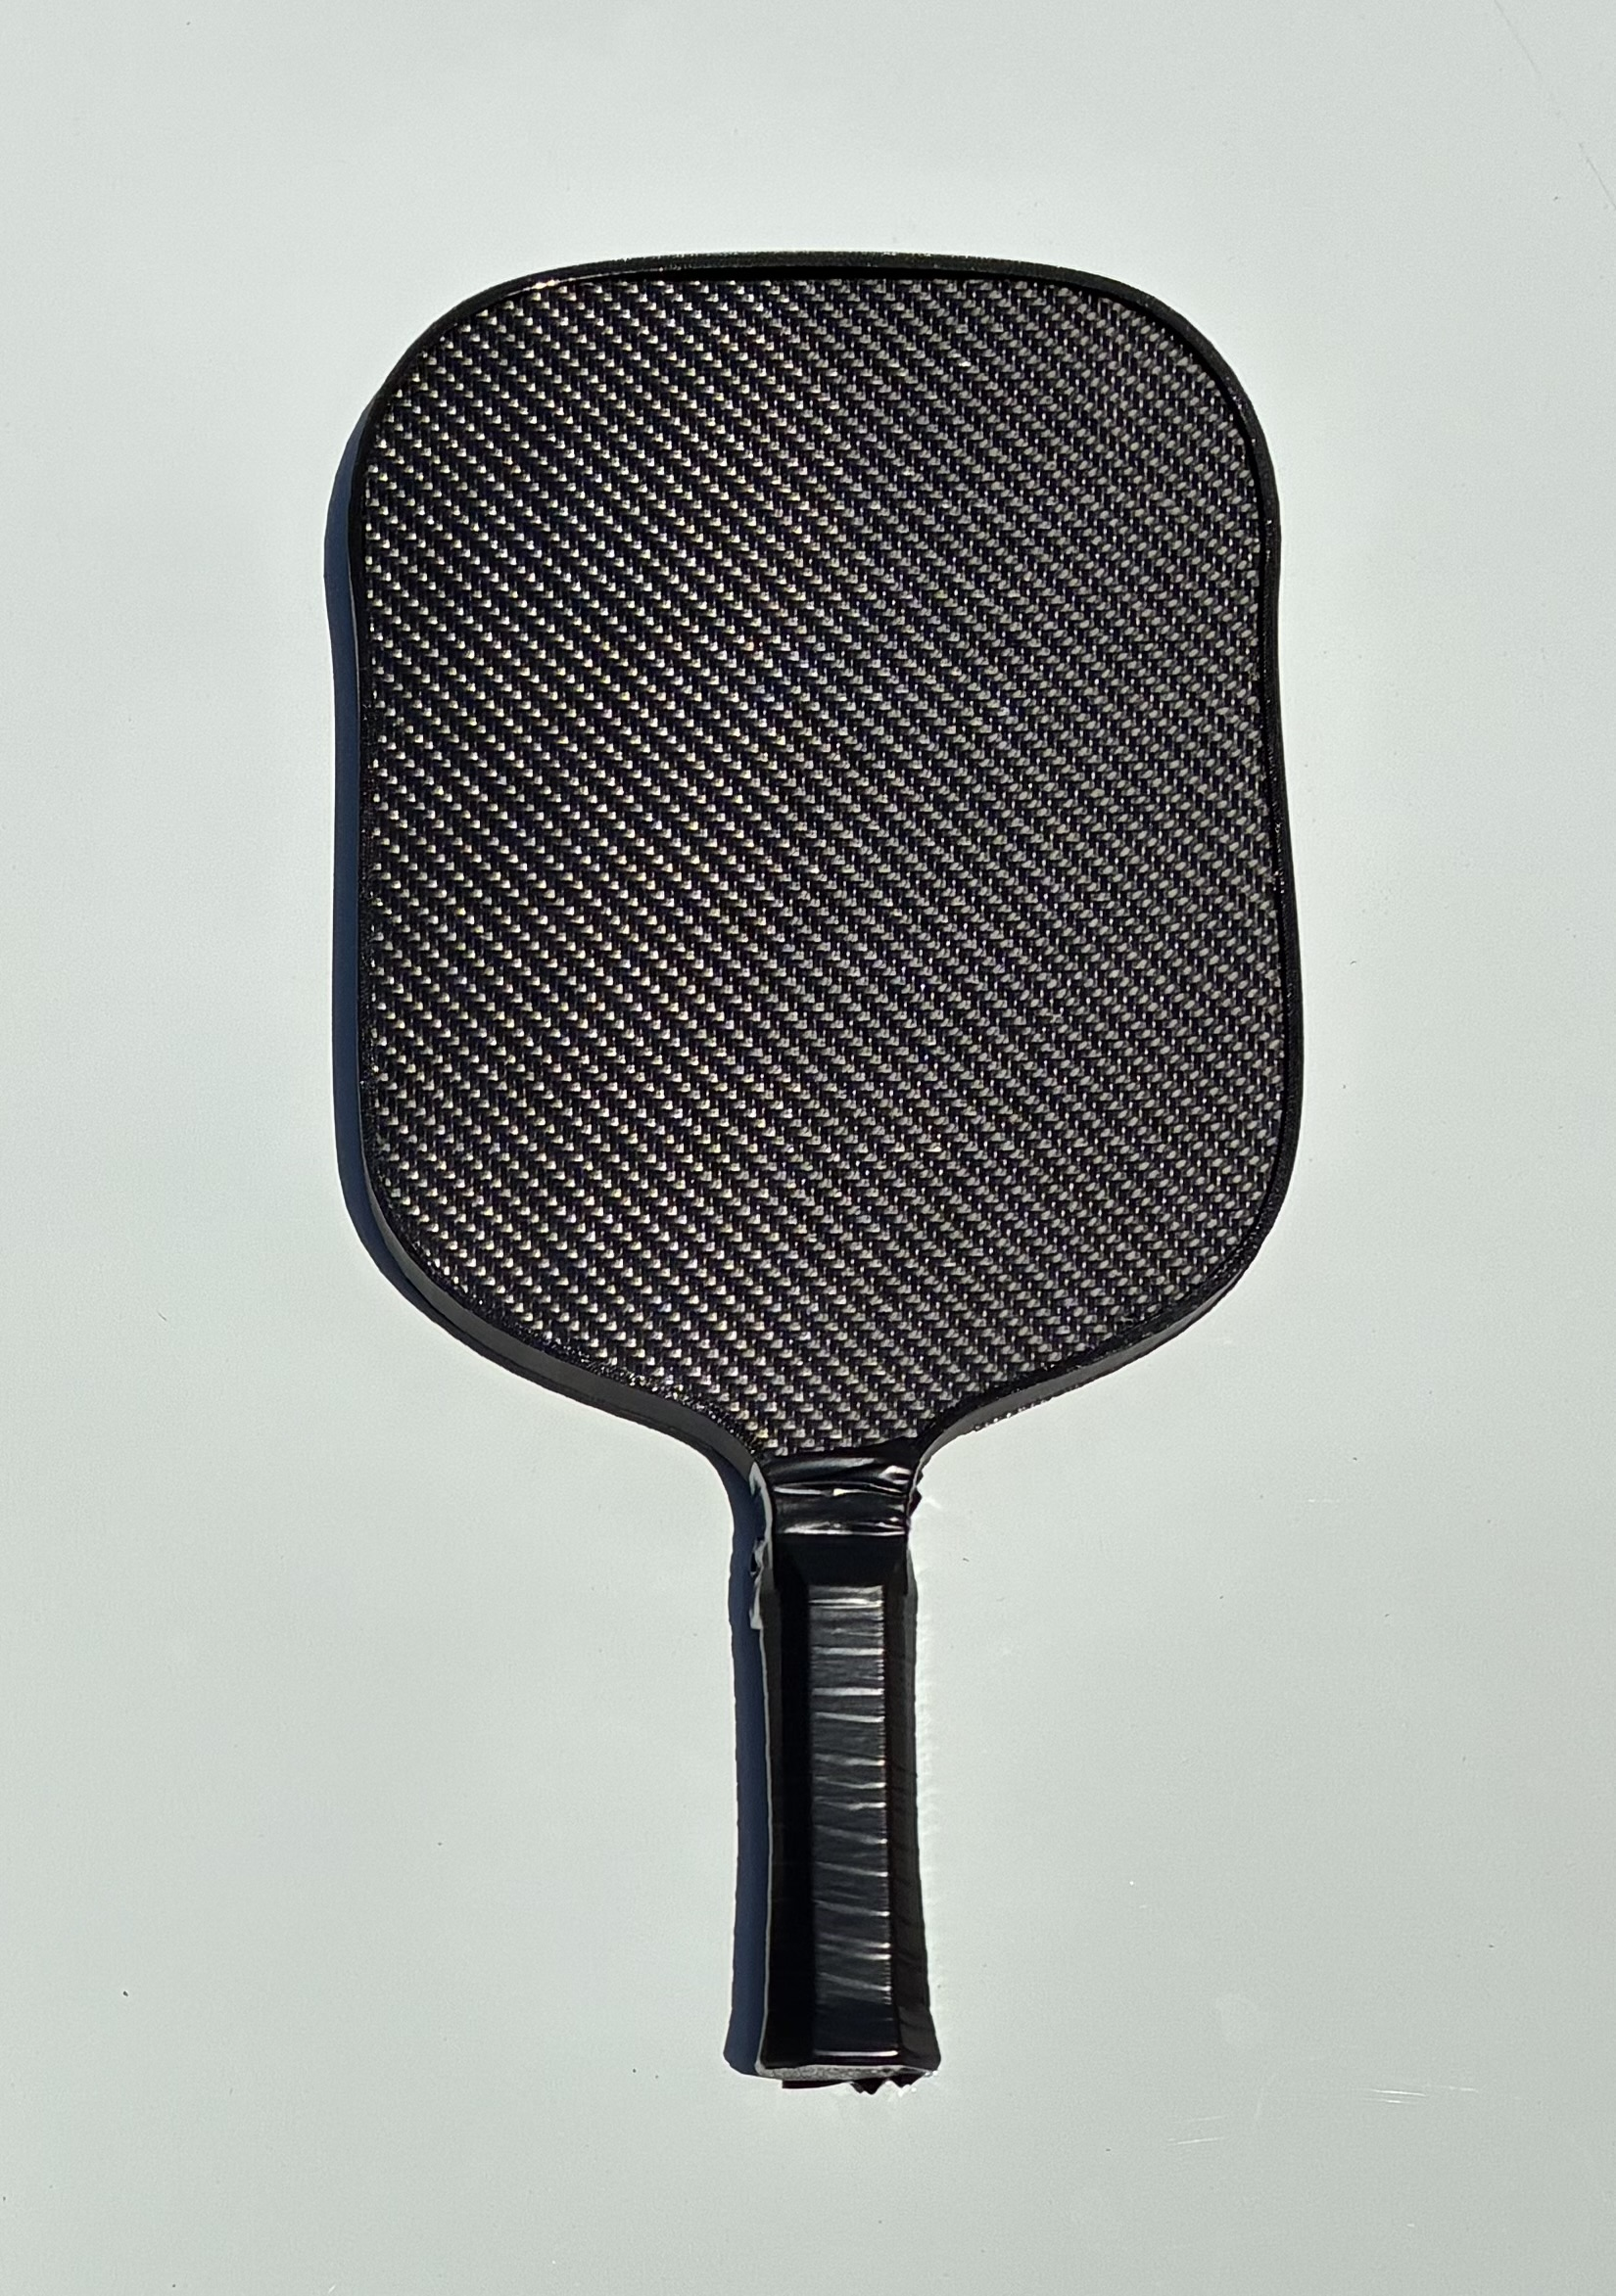
\includegraphics[
        width=3.72in,
        height=3.18in,
        keepaspectratio
    ]{full_assy}
};

\node[
    anchor=north,
    text=Muted,
    font=\sffamily\fontsize{6.9}{7.5}\selectfont
]
at ($(current page.north west)+(1.60in,-4.86in)$)
{Completed solo-built paddle assembly};

% ============================================================
% TOP CENTER — PROJECT OVERVIEW
% ============================================================

\fill[SoftGold,rounded corners=5pt]
    ($(current page.north west)+(2.95in,-1.62in)$)
    rectangle
    ($(current page.north west)+(5.53in,-4.86in)$);

\fill[PolyGold]
    ($(current page.north west)+(2.95in,-1.62in)$)
    rectangle
    ($(current page.north west)+(3.05in,-4.86in)$);

\node[
    anchor=north west,
    text=DeepGreen,
    font=\sffamily\bfseries\fontsize{8.0}{8.7}\selectfont
]
at ($(current page.north west)+(3.23in,-1.79in)$)
{PROJECT OVERVIEW};

\node[
    anchor=north west,
    align=left,
    text width=2.02in,
    text=Ink,
    font=\fontsize{7.05}{8.35}\selectfont
]
at ($(current page.north west)+(3.23in,-2.07in)$)
{
Independently designed and manufactured a lightweight prepreg
carbon-fiber pickleball paddle using a half-inch honeycomb
sandwich core, vacuum-bag consolidation, precision waterjet
trimming, and custom TPU and PLA components.

\vspace{5pt}

The project emphasized lightweight sandwich-composite design, repeatable manufacturing methods, dimensional accuracy, and the integration of custom 3D-printed TPU and PLA components into the final assembly.
};

\node[
    anchor=south west,
    align=left,
    text width=2.02in,
    text=PolyGold,
    font=\sffamily\bfseries\fontsize{6.65}{7.35}\selectfont
]
at ($(current page.north west)+(3.23in,-4.74in)$)
{
SOLE DESIGNER\\[2pt]
COMPOSITE FABRICATOR\\[2pt]
MANUFACTURING ENGINEER
};

% ============================================================
% TOP RIGHT — LAMINATE GRAPHIC
% ============================================================

\node[
    anchor=north west,
    inner sep=2.5pt,
    draw=DeepGreen,
    line width=0.65pt,
    rounded corners=5pt
]
at ($(current page.north west)+(5.71in,-1.62in)$)
{
    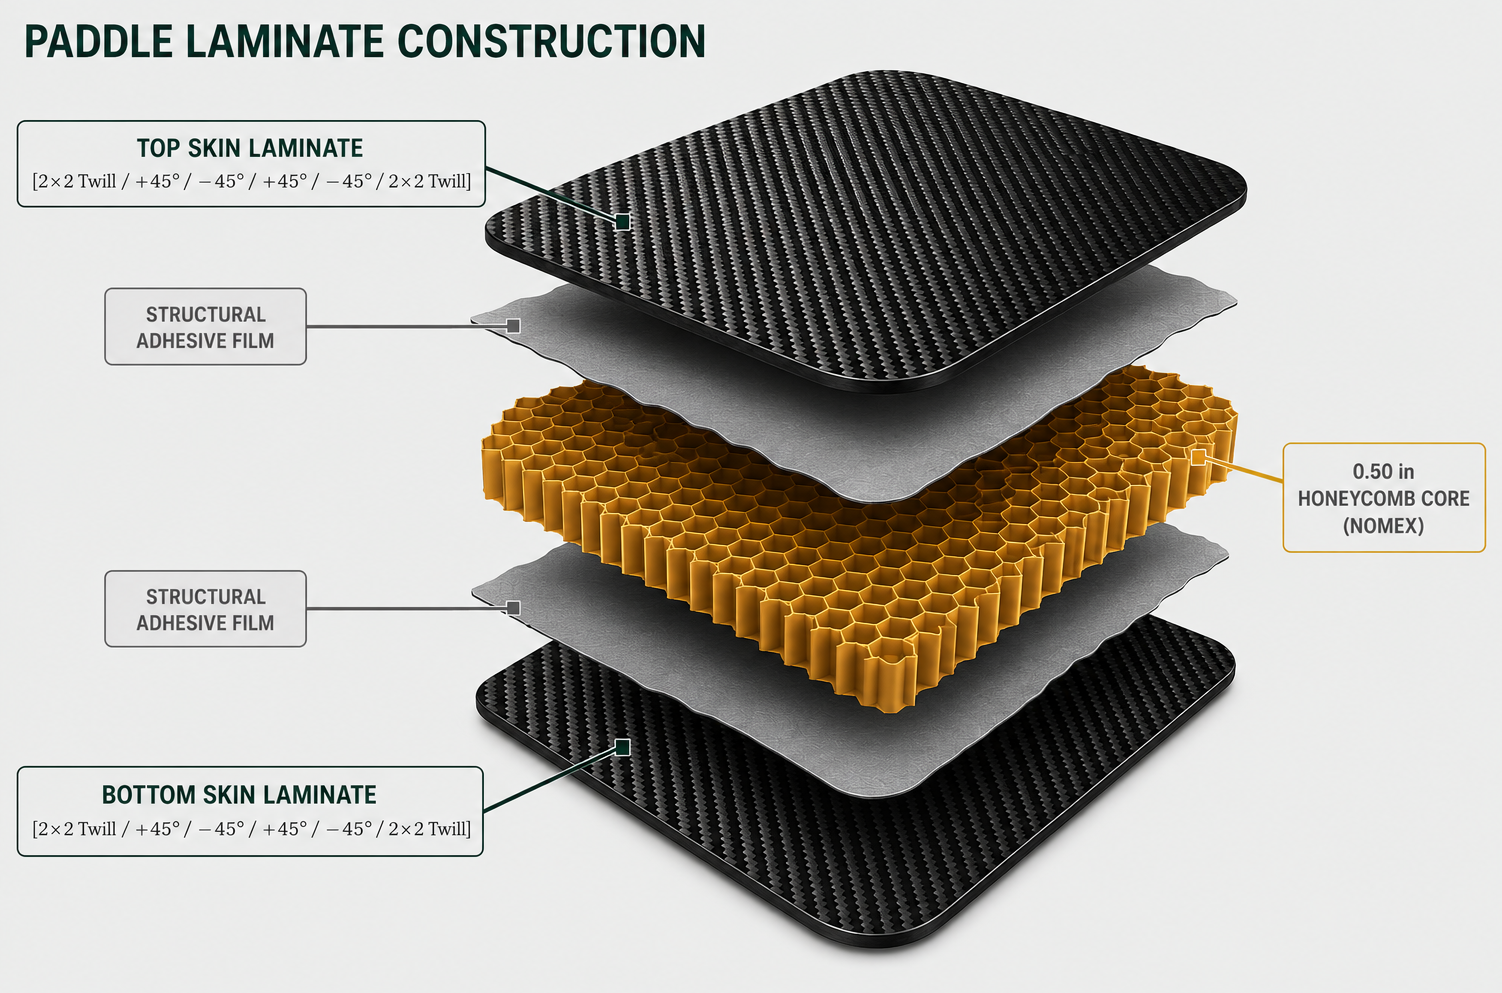
\includegraphics[
        width=4.80in,
        keepaspectratio
    ]{LAMINATE}
};

% ============================================================
% BOTTOM LEFT — SUPPORTING IMAGES
% ============================================================

\node[
    anchor=center,
    inner sep=3pt,
    draw=RuleGray,
    line width=0.55pt,
    rounded corners=4pt
]
at ($(current page.north west)+(1.12in,-5.98in)$)
{
    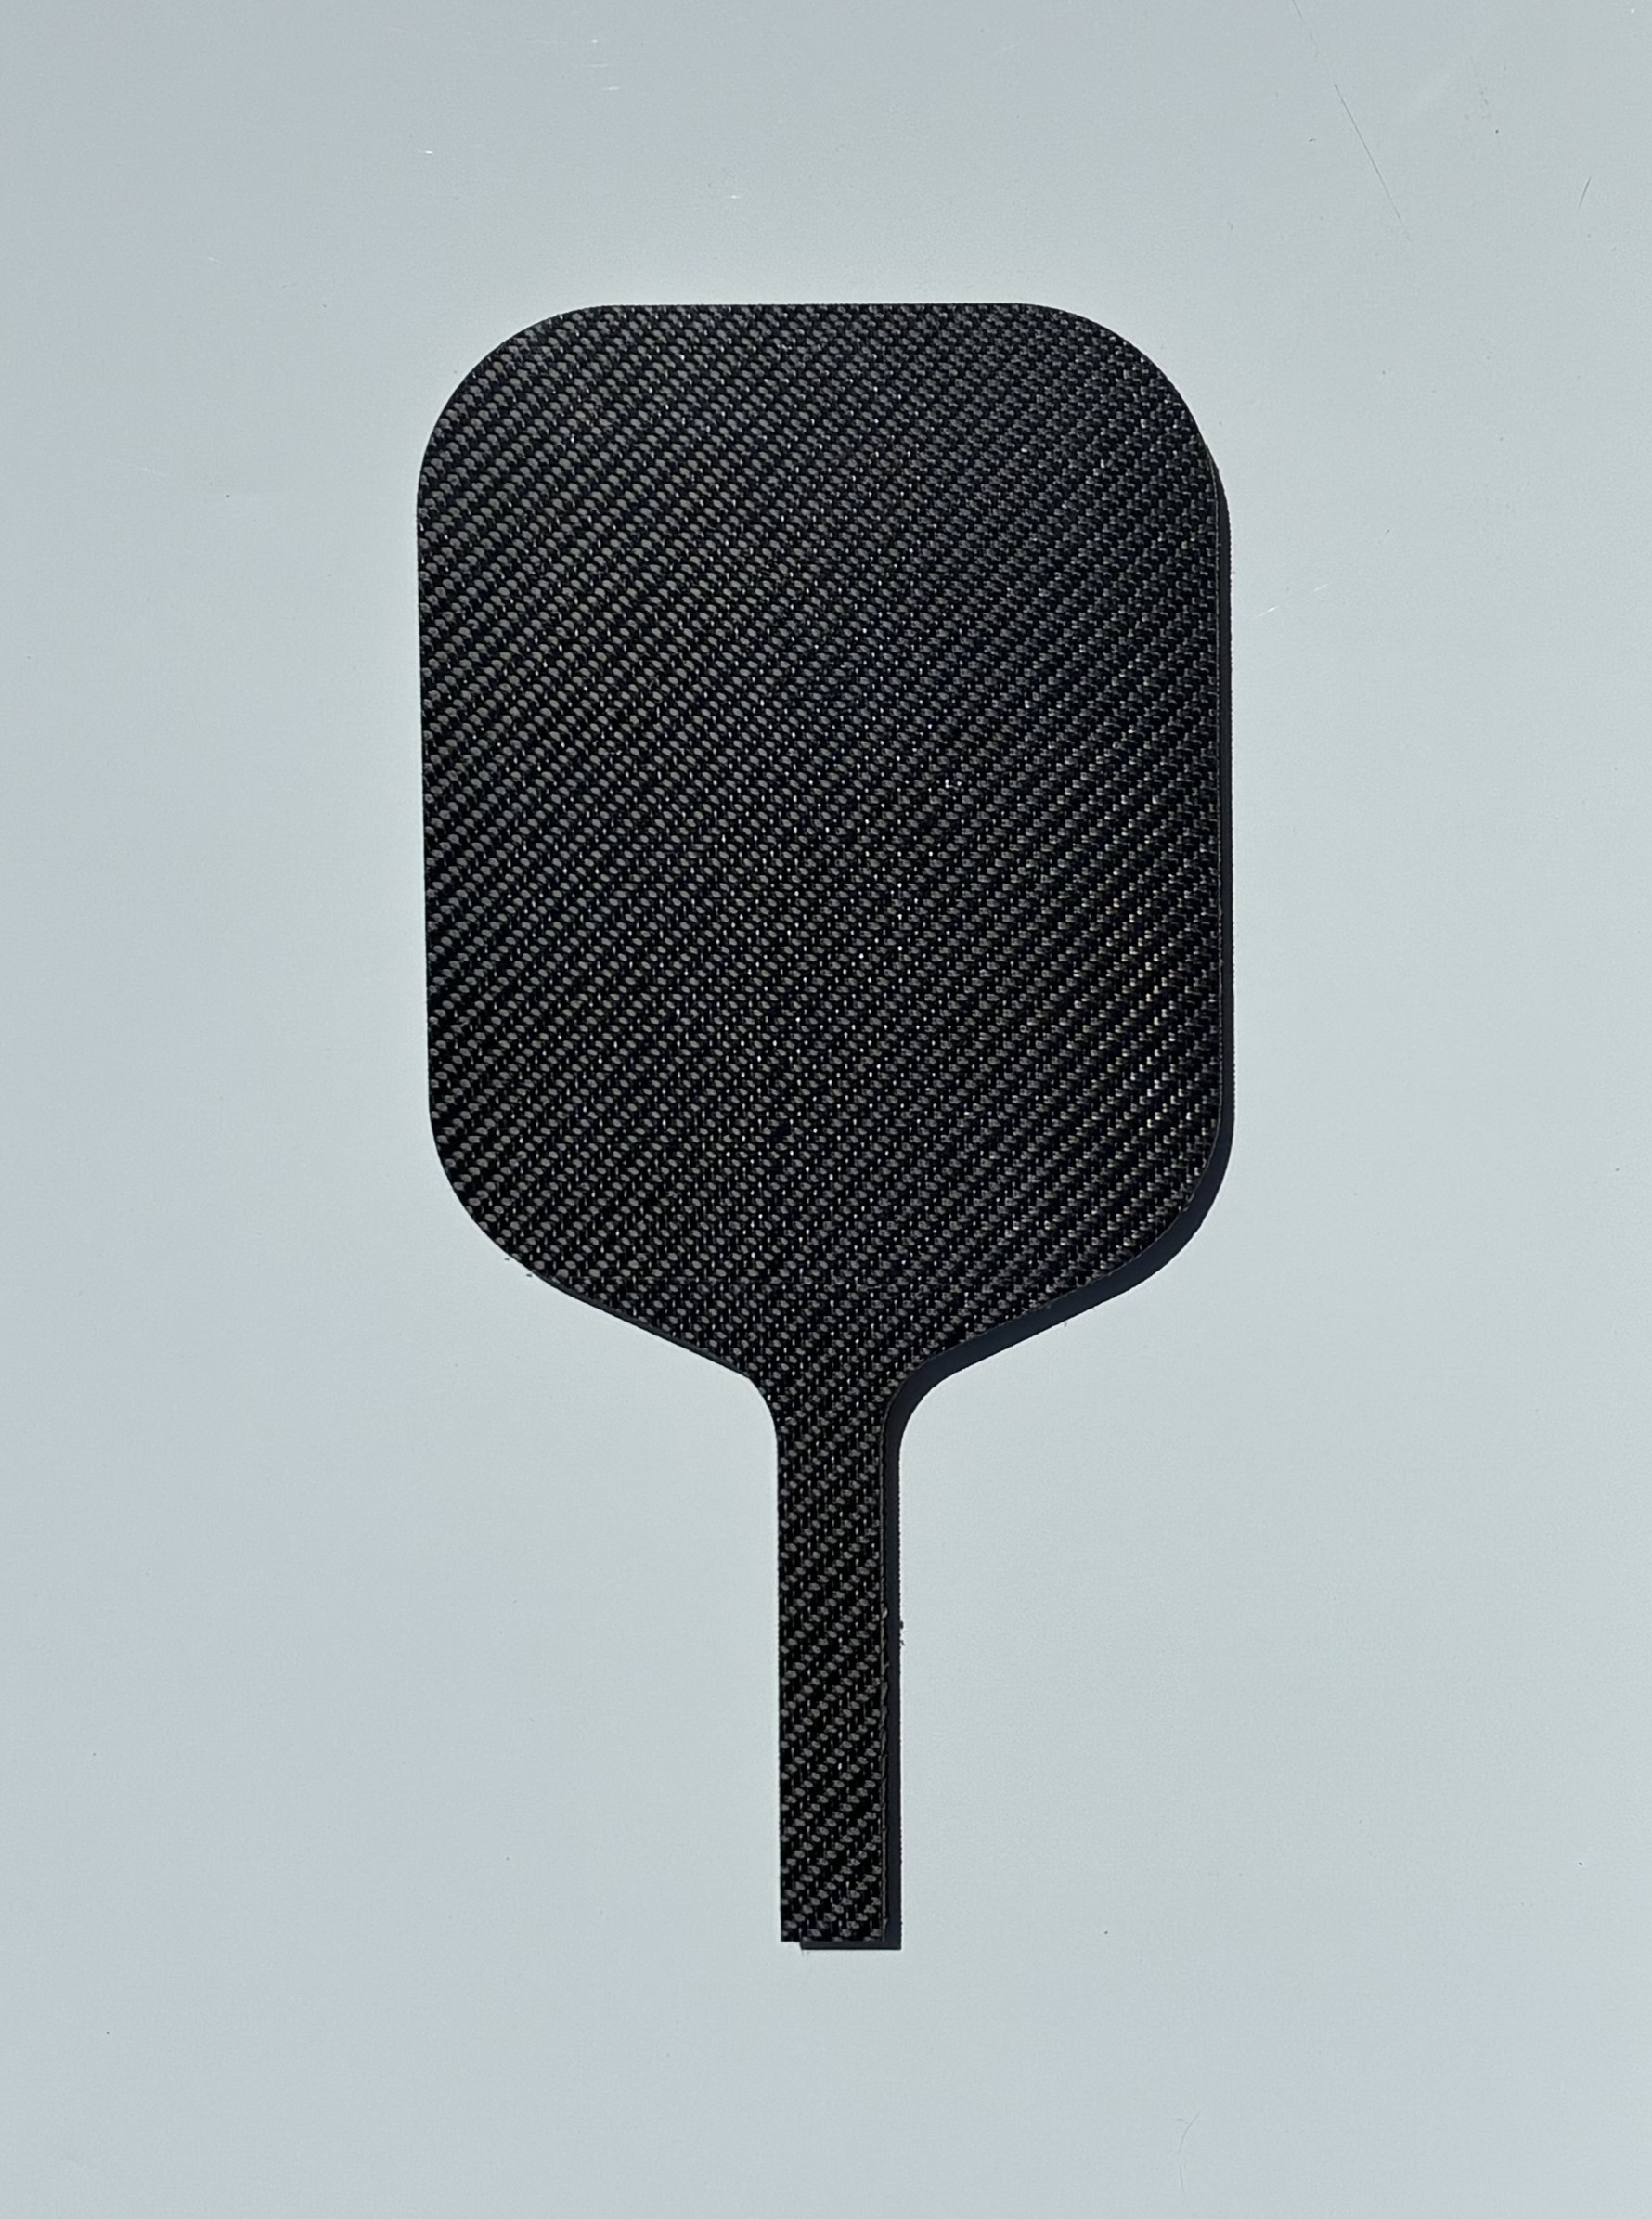
\includegraphics[
        width=1.30in,
        height=1.78in,
        keepaspectratio
    ]{front_view}
};

\node[
    anchor=center,
    inner sep=3pt,
    draw=RuleGray,
    line width=0.55pt,
    rounded corners=4pt
]
at ($(current page.north west)+(2.72in,-5.98in)$)
{
    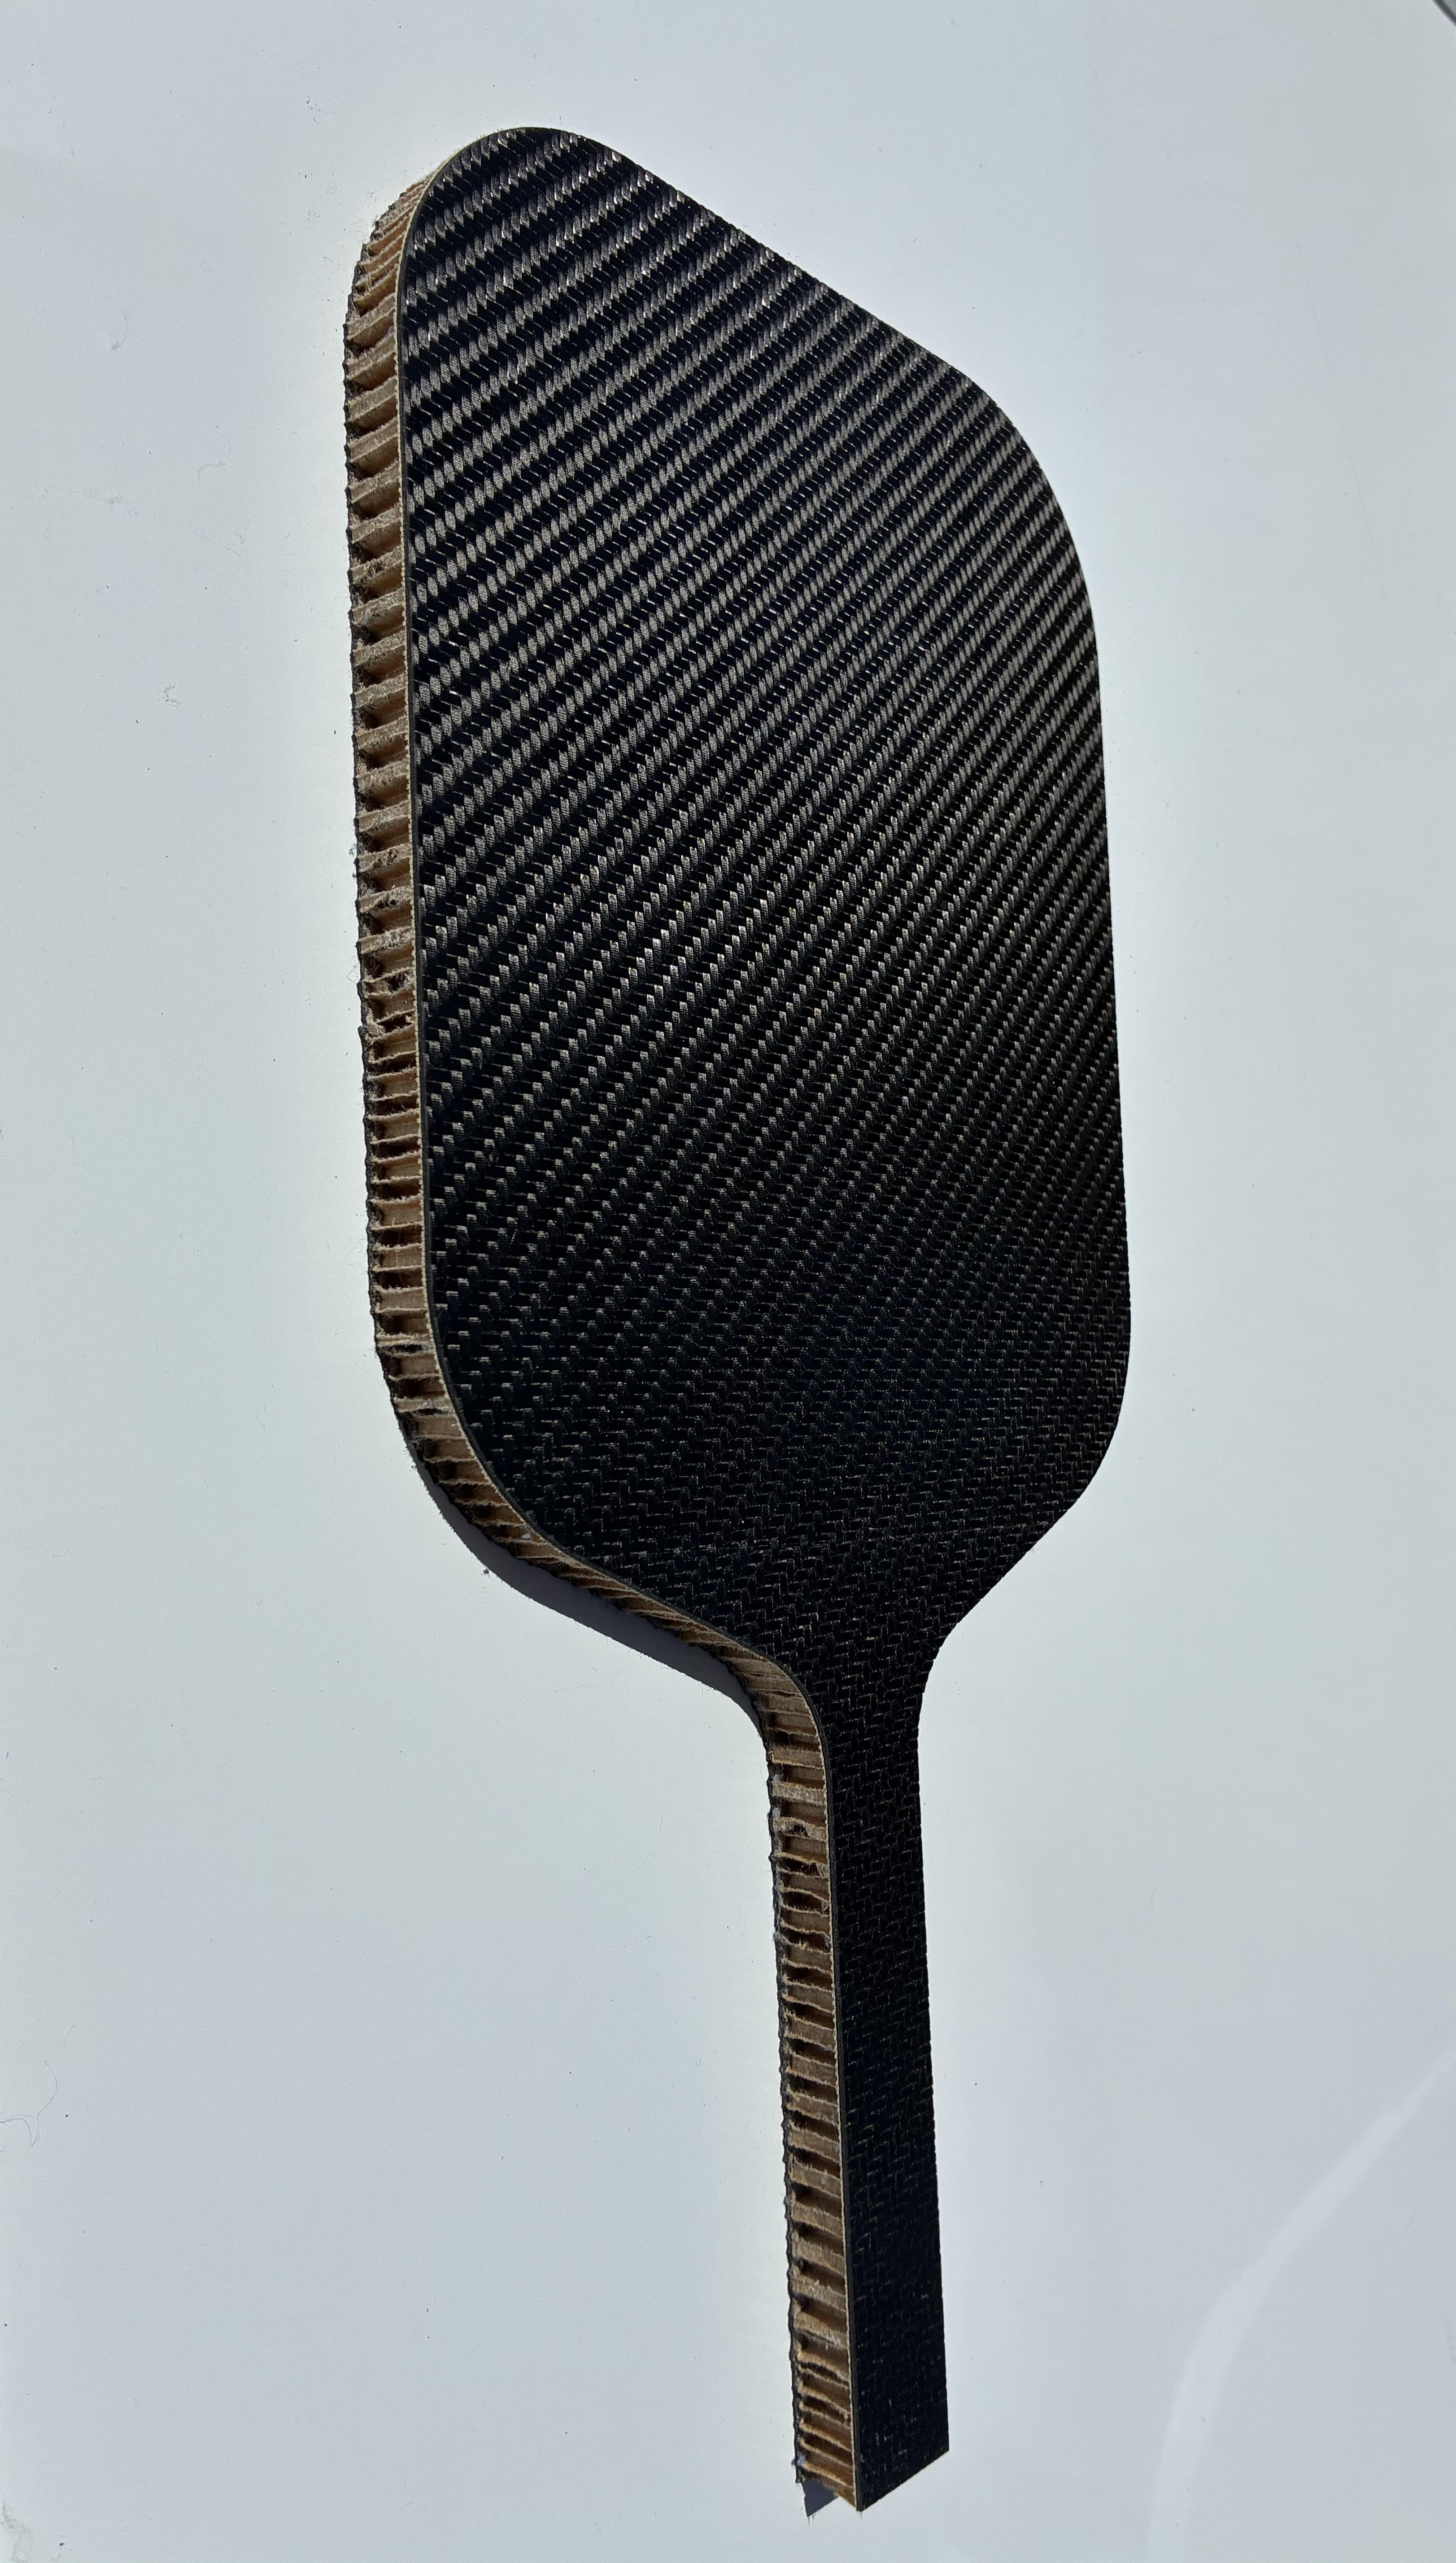
\includegraphics[
        width=1.30in,
        height=1.78in,
        keepaspectratio
    ]{side_core_view}
};

\node[
    anchor=center,
    inner sep=3pt,
    draw=RuleGray,
    line width=0.55pt,
    rounded corners=4pt
]
at ($(current page.north west)+(4.32in,-5.98in)$)
{
    \includegraphics[
        angle=-90,
        origin=c,
        width=1.30in,
        height=1.78in,
        keepaspectratio
    ]{waterjet}
};

\node[
    anchor=north,
    align=center,
    text width=1.38in,
    text=Muted,
    font=\sffamily\fontsize{6.5}{7.1}\selectfont
]
at ($(current page.north west)+(1.12in,-7.00in)$)
{Front view};

\node[
    anchor=north,
    align=center,
    text width=1.38in,
    text=Muted,
    font=\sffamily\fontsize{6.5}{7.1}\selectfont
]
at ($(current page.north west)+(2.72in,-7.00in)$)
{Core and edge profile};

\node[
    anchor=north,
    align=center,
    text width=1.38in,
    text=Muted,
    font=\sffamily\fontsize{6.5}{7.1}\selectfont
]
at ($(current page.north west)+(4.32in,-7.00in)$)
{Waterjet cutting setup};

% ============================================================
% BOTTOM RIGHT — MANUFACTURING HIGHLIGHTS
% ============================================================

\fill[SoftGreen,rounded corners=5pt]
    ($(current page.north west)+(5.18in,-5.05in)$)
    rectangle
    ($(current page.north east)+(-0.42in,-7.18in)$);

\draw[RuleGray,line width=0.55pt,rounded corners=5pt]
    ($(current page.north west)+(5.18in,-5.05in)$)
    rectangle
    ($(current page.north east)+(-0.42in,-7.18in)$);

\node[
    anchor=north west,
    text=DeepGreen,
    font=\sffamily\bfseries\fontsize{7.9}{8.6}\selectfont
]
at ($(current page.north west)+(5.44in,-5.20in)$)
{MANUFACTURING HIGHLIGHTS};

\node[
    anchor=north west,
    align=left,
    text width=5.05in,
    text=Ink,
    font=\fontsize{6.72}{7.82}\selectfont
]
at ($(current page.north west)+(5.44in,-5.49in)$)
{
\textbf{Consolidation.}
Vacuum bagging and distributed weight pressure maintained intimate contact
throughout the prepreg sandwich layup.\\[2.4pt]
\textbf{Surface quality.}
A scarce PTFE release film produced an unusually consistent matte finish
with a subtle sheen and minimal post-processing.\\[2.4pt]
\textbf{Waterjet stability.}
Perimeter weights restrained the cured stock against jet-induced lifting
and rotational moments during cutting.\\[2.4pt]
\textbf{Final assembly.}
A printed TPU edge band protected the carbon perimeter, while the PLA handle
used clearance cutouts to accommodate future stock-thickness and cutting variation.
};

% ============================================================
% RESOURCE LINK
% ============================================================

\node[
    anchor=north,
    align=center,
    text=DeepGreen,
    font=\sffamily\bfseries\fontsize{7.0}{7.6}\selectfont
]
at ($(current page.north)+(0,-7.42in)$)
{\href{\PaddleWaterjetVideo}
{\faPlayCircle\ WATERJET PICKLEBALL PADDLE DEMONSTRATION}};

% ============================================================
% FOOTER
% ============================================================

\node[
    anchor=south west,
    text=white,
    font=\sffamily\bfseries\fontsize{7.1}{7.7}\selectfont
]
at ($(current page.south west)+(0.42in,0.17in)$)
{\hyperlink{toro-results}{\faArrowLeft\ TORO COVER}};

\node[
    anchor=south,
    text=white,
    font=\sffamily\fontsize{7.0}{7.6}\selectfont
]
at ($(current page.south)+(0,0.17in)$)
{PICKLEBALL PADDLE \hspace{6pt} 1 / 1};

\node[
    anchor=south east,
    text=white,
    font=\sffamily\bfseries\fontsize{7.1}{7.7}\selectfont
]
at ($(current page.south east)+(-0.42in,0.17in)$)
{NEXT PROJECT \faArrowRight};

\end{tikzpicture}
%\input{Beam}
%\clearpage

\clearpage
 before \end{document}.
% 3. Image references use the original Overleaf base filenames
%    without extensions.
% ============================================================



% ============================================================
% CLICKABLE PROJECT RESOURCES
% All links use the exact Google Drive resources supplied.
% ============================================================
\providecommand{\ToroDrawingLink}{https://drive.google.com/file/d/1A7-7wMnRNLuQDaTgxeuUCBsGNqyXzOGV/view?usp=sharing}
\providecommand{\ToroDimensionsLink}{https://drive.google.com/file/d/13sw3BNJvE8GdzlRffxoF2n5r9Gzxide7/view?usp=sharing}
\providecommand{\ToroProblemLink}{https://drive.google.com/file/d/1zHtl8zrb13F1yeN74ptawpfS5UM_xsuw/view?usp=drive_link}
\providecommand{\ToroReportLink}{https://drive.google.com/file/d/1ULZ-P46lFsC2x29ZfmRVIKgYnr9o8hMt/view?usp=drive_link}
\providecommand{\ToroPosterLink}{https://drive.google.com/file/d/1vKiKaJUcHQb_db-FkZnRF6EvtuM4hKyS/view?usp=drive_link}
\providecommand{\ToroDeploymentLink}{https://drive.google.com/file/d/1XJx34o80_mZPTl7xy93HtWAgtS3ThhvY/view?usp=drive_link}
\providecommand{\ToroRemovalLink}{https://drive.google.com/file/d/1O7xYeyB67NUwT-j1B1HeiCcHnZDYjk6_/view?usp=drive_link}

% ============================================================
% PAGE 1 — PROJECT OVERVIEW, OWNERSHIP, AND ARCHITECTURE
% ============================================================

\clearpage
\thispagestyle{empty}
\hypertarget{toro}{}
\null

\begin{tikzpicture}[remember picture,overlay]

% Background
\fill[white]
    (current page.south west)
    rectangle
    (current page.north east);

% Page bars
\fill[DeepGreen]
    (current page.north west)
    rectangle
    ($(current page.north east)+(0,-0.095in)$);

\fill[PolyGold]
    ($(current page.north west)+(0,-0.095in)$)
    rectangle
    ($(current page.north east)+(0,-0.14in)$);

\fill[DeepGreen]
    (current page.south west)
    rectangle
    ($(current page.south east)+(0,0.36in)$);

\fill[PolyGold]
    ($(current page.south west)+(0,0.36in)$)
    rectangle
    ($(current page.south east)+(0,0.405in)$);

% Header
\node[
    anchor=north west,
    text=PolyGold,
    font=\sffamily\bfseries\fontsize{8.1}{8.7}\selectfont
]
at ($(current page.north west)+(0.42in,-0.39in)$)
{01 COMPOSITES \hspace{5pt}/\hspace{5pt} PROJECT 01};

\node[
    anchor=north west,
    text=DeepGreen,
    font=\bfseries\fontsize{23.5}{24.5}\selectfont
]
at ($(current page.north west)+(0.40in,-0.67in)$)
{TORO CARBON FIBER SAFETY COVER};

\node[
    anchor=north west,
    text=Muted,
    font=\sffamily\fontsize{8.4}{9.2}\selectfont
]
at ($(current page.north west)+(0.42in,-1.12in)$)
{Cal Poly Composites Laboratory \hspace{7pt}\textbullet\hspace{7pt}
Team Project \hspace{7pt}\textbullet\hspace{7pt}
Fall--Spring 2026 \hspace{7pt}\textbullet\hspace{7pt}
San Luis Obispo, California};

\fill[PolyGold]
    ($(current page.north west)+(0.42in,-1.37in)$)
    rectangle
    ($(current page.north west)+(6.1in,-1.325in)$);

% Challenge text
\node[
    anchor=north west,
    text=DeepGreen,
    font=\sffamily\bfseries\fontsize{8.1}{8.8}\selectfont
]
at ($(current page.north west)+(0.43in,-1.61in)$)
{THE CHALLENGE};

\node[
    anchor=north west,
    align=left,
    text width=4.47in,
    text=Ink,
    font=\fontsize{8.05}{9.65}\selectfont
]
at ($(current page.north west)+(0.43in,-1.84in)$)
{
Develop a lightweight cover for a 6 ft by 6 ft in-ground spa
that could be deployed by one person, stored compactly,
provide insulation, resist a poolside environment, and maintain
a refined appearance. The sponsor supplied an ambitious but
intentionally broad project statement, requiring the team to
define the product architecture, priorities, manufacturing
strategy, and realistic path toward future commercialization.
};

% Role box
\fill[SoftGold,rounded corners=5pt]
    ($(current page.north west)+(0.42in,-2.88in)$)
    rectangle
    ($(current page.north west)+(4.98in,-4.58in)$);

\fill[PolyGold]
    ($(current page.north west)+(0.42in,-2.88in)$)
    rectangle
    ($(current page.north west)+(0.52in,-4.58in)$);

\node[
    anchor=north west,
    text=DeepGreen,
    font=\sffamily\bfseries\fontsize{8.1}{8.8}\selectfont
]
at ($(current page.north west)+(0.66in,-3.02in)$)
{MY ROLE — DESIGN \& MANUFACTURING LEAD};

\node[
    anchor=north west,
    align=left,
    text width=4.02in,
    text=Ink,
    font=\fontsize{7.05}{8.15}\selectfont
]
at ($(current page.north west)+(0.66in,-3.27in)$)
{
\textbullet\ Modeled every custom part and the complete assembly\\[1.5pt]
\textbullet\ Produced the engineering drawing package independently\\[1.5pt]
\textbullet\ Developed the composite-panel manufacturing process\\[1.5pt]
\textbullet\ Created all waterjet DXFs and manufacturing geometry\\[1.5pt]
\textbullet\ Trained teammates in wet layup and vacuum bagging\\[1.5pt]
\textbullet\ Presented feasibility, scope, and tradeoffs to the sponsor
};

% Large deployed foam-model image
\node[anchor=center,inner sep=0pt]
at ($(current page.north west)+(8.00in,-3.04in)$)
{
    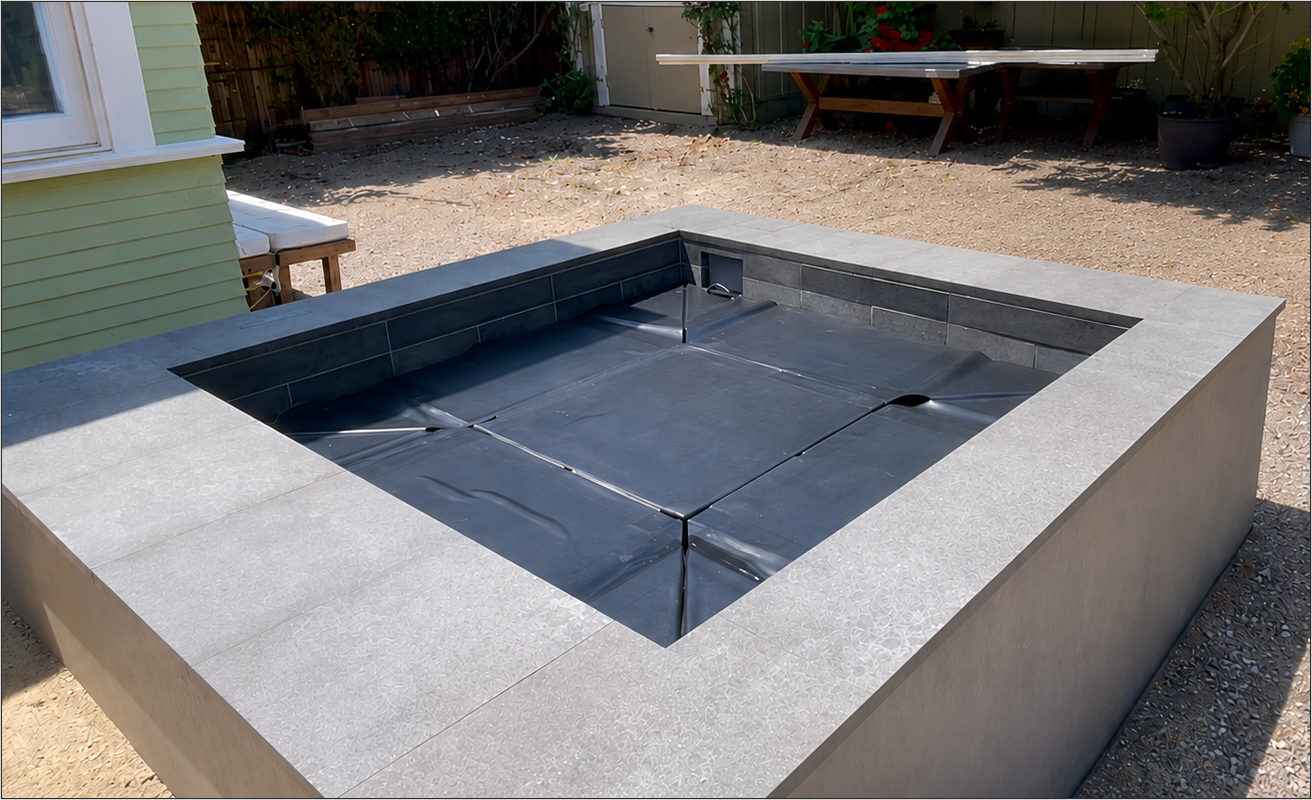
\includegraphics[
        width=5.55in,
        height=2.78in,
        keepaspectratio
    ]{deployed_functional_prototype}
};

\draw[DeepGreen,line width=0.8pt,rounded corners=7pt]
    ($(current page.north west)+(5.16in,-1.61in)$)
    rectangle
    ($(current page.north east)+(-0.42in,-4.47in)$);

\node[
    anchor=north west,
    text=Muted,
    font=\sffamily\fontsize{6.2}{6.9}\selectfont
]
at ($(current page.north west)+(5.18in,-4.54in)$)
{Functional foam model deployed over the sponsor's in-ground spa.};

% Image-strip title
\node[
    anchor=north west,
    text=DeepGreen,
    font=\sffamily\bfseries\fontsize{8.1}{8.8}\selectfont
]
at ($(current page.north west)+(0.43in,-4.78in)$)
{PRODUCT DEVELOPMENT AND FINAL ARCHITECTURE};

% Five-image development strip — CAD-first sequence
% Image 1: topside CAD
\node[anchor=center,inner sep=0pt]
at ($(current page.north west)+(1.47in,-5.73in)$)
{
    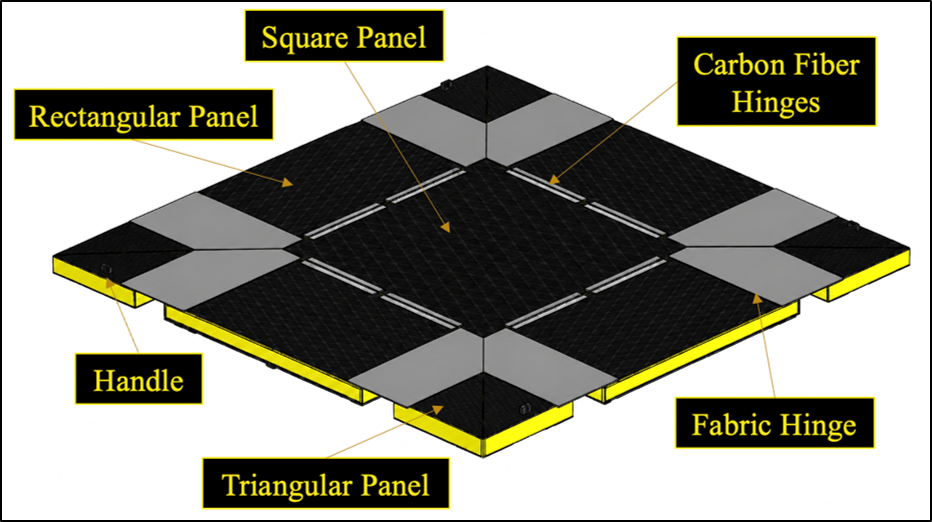
\includegraphics[
        width=1.92in,
        height=1.30in,
        keepaspectratio
    ]{Toro_Cover_topside_Cad}
};
\draw[RuleGray,line width=0.55pt,rounded corners=4pt]
    ($(current page.north west)+(0.43in,-5.04in)$)
    rectangle
    ($(current page.north west)+(2.51in,-6.43in)$);

% Image 2: underside CAD
\node[anchor=center,inner sep=0pt]
at ($(current page.north west)+(3.66in,-5.73in)$)
{
    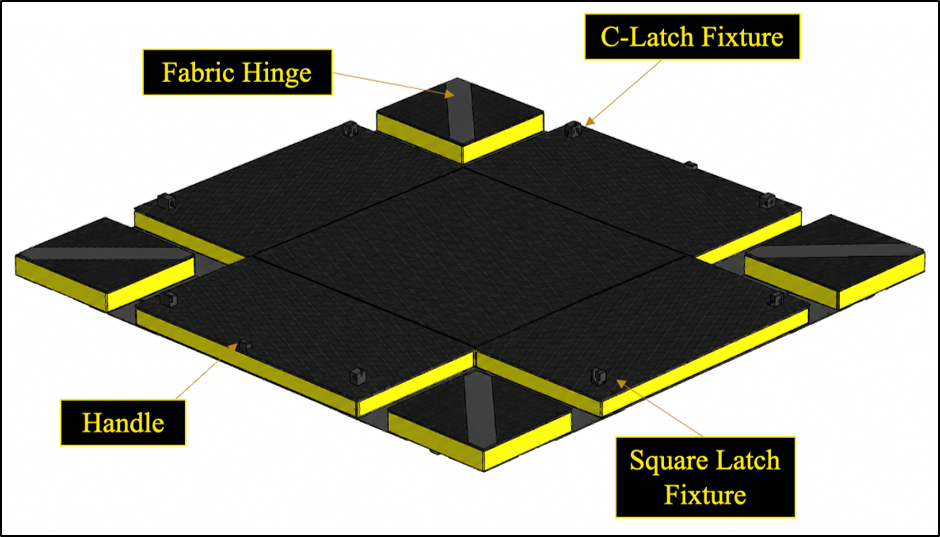
\includegraphics[
        width=1.92in,
        height=1.30in,
        keepaspectratio
    ]{toro_cover_underside_cad}
};
\draw[RuleGray,line width=0.55pt,rounded corners=4pt]
    ($(current page.north west)+(2.62in,-5.04in)$)
    rectangle
    ($(current page.north west)+(4.70in,-6.43in)$);

% Image 3: folded CAD
\node[anchor=center,inner sep=0pt]
at ($(current page.north west)+(5.85in,-5.73in)$)
{
    \includegraphics[
        width=1.92in,
        height=1.30in,
        keepaspectratio
    ]{\detokenize{Toro_Cover_folded Configuration}}
};
\draw[RuleGray,line width=0.55pt,rounded corners=4pt]
    ($(current page.north west)+(4.81in,-5.04in)$)
    rectangle
    ($(current page.north west)+(6.89in,-6.43in)$);

% Image 4: dual-use product concept
\node[anchor=center,inner sep=0pt]
at ($(current page.north west)+(8.04in,-5.73in)$)
{
    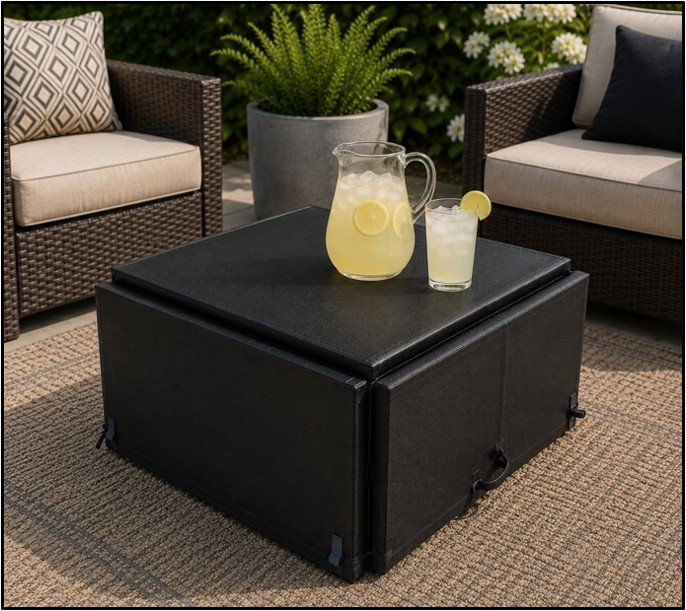
\includegraphics[
        width=1.92in,
        height=1.30in,
        keepaspectratio
    ]{generative_AI_concept_toro_cover_art}
};
\draw[RuleGray,line width=0.55pt,rounded corners=4pt]
    ($(current page.north west)+(7.00in,-5.04in)$)
    rectangle
    ($(current page.north west)+(9.08in,-6.43in)$);

% Image 5: folded foam functional prototype
% The portrait photograph is deliberately clipped to the landscape frame
% so the ottoman fills the card without extending beyond its border.
\begin{scope}
\clip[rounded corners=4pt]
    ($(current page.north west)+(9.19in,-5.04in)$)
    rectangle
    ($(current page.north east)+(-0.43in,-6.43in)$);

% Keep the original image proportions and center it within the existing card.
\node[anchor=center,inner sep=0pt]
at ($(current page.north west)+(9.88in,-5.735in)$)
{
    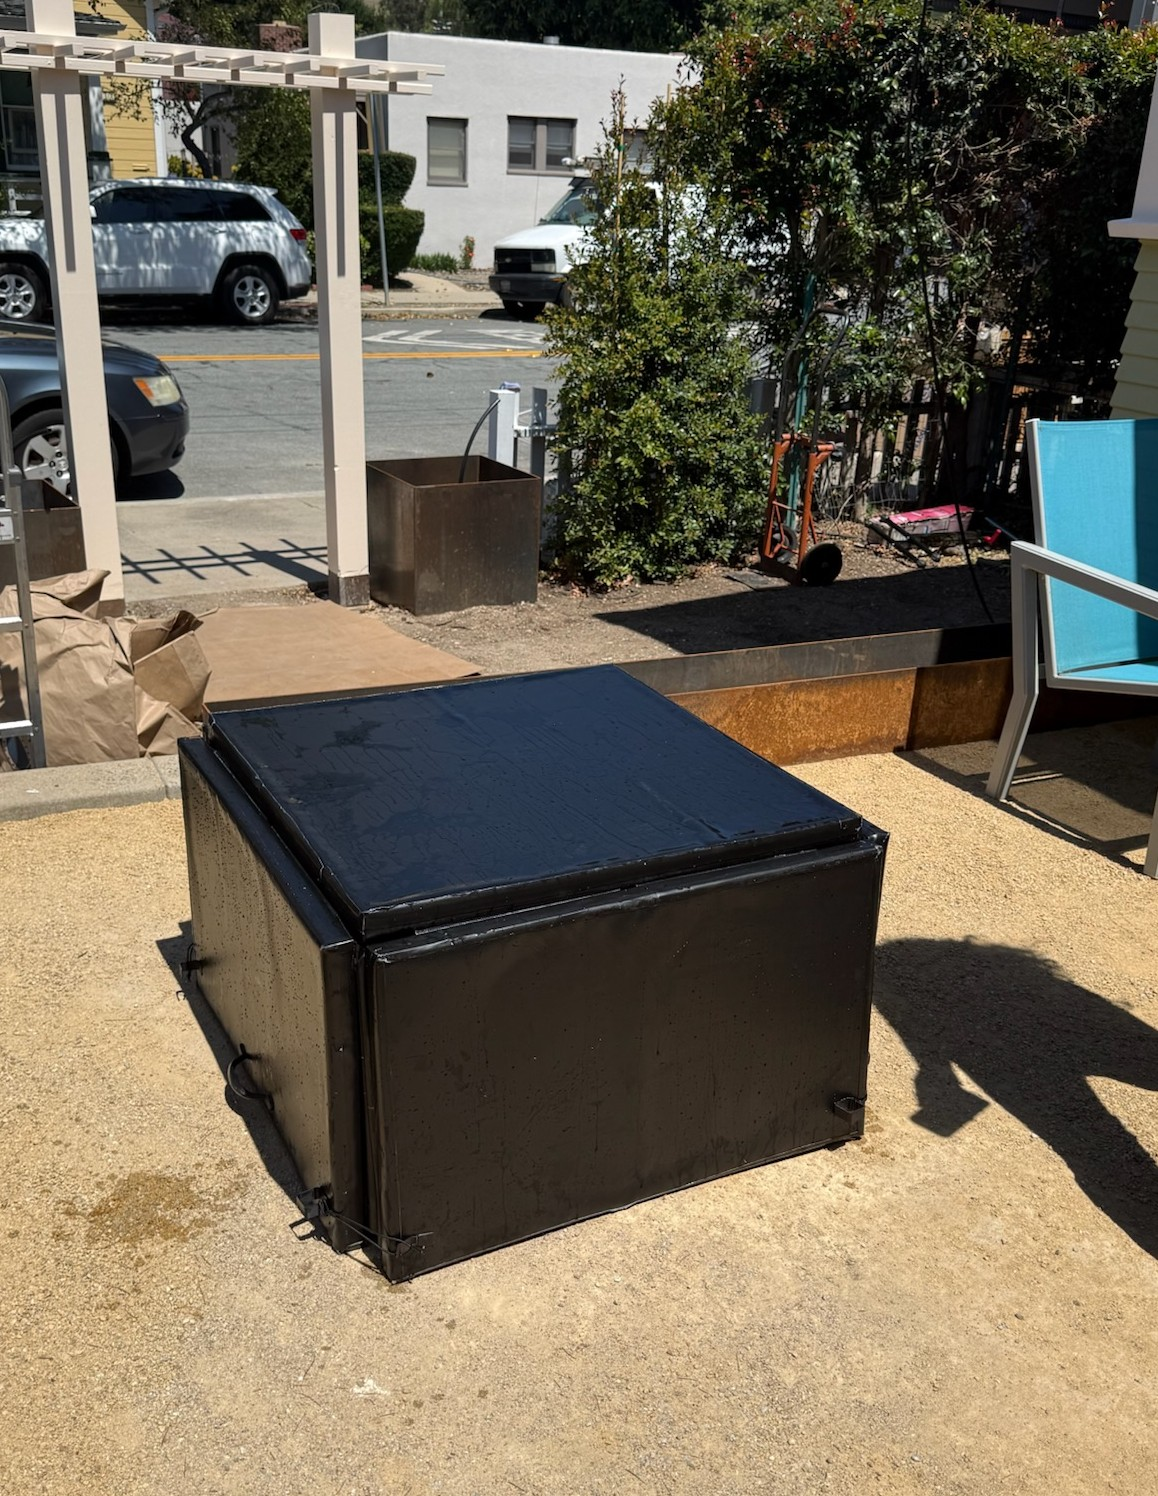
\includegraphics[
        width=1.58in,
        height=1.28in,
        keepaspectratio
    ]{foam_model_folded_backyard_image}
};
\end{scope}

\draw[RuleGray,line width=0.55pt,rounded corners=4pt]
    ($(current page.north west)+(9.19in,-5.04in)$)
    rectangle
    ($(current page.north east)+(-0.43in,-6.43in)$);

% Larger captions
\node[anchor=north,align=center,text width=1.95in,text=Muted,
      font=\sffamily\fontsize{6.8}{7.4}\selectfont]
at ($(current page.north west)+(1.47in,-6.49in)$)
{Topside panel architecture};

\node[anchor=north,align=center,text width=1.95in,text=Muted,
      font=\sffamily\fontsize{6.8}{7.4}\selectfont]
at ($(current page.north west)+(3.66in,-6.49in)$)
{Underside hinge architecture};

\node[anchor=north,align=center,text width=1.95in,text=Muted,
      font=\sffamily\fontsize{6.8}{7.4}\selectfont]
at ($(current page.north west)+(5.85in,-6.49in)$)
{Folded CAD configuration};

\node[anchor=north,align=center,text width=1.95in,text=Muted,
      font=\sffamily\fontsize{6.8}{7.4}\selectfont]
at ($(current page.north west)+(8.04in,-6.49in)$)
{Dual-use product vision};

\node[anchor=north,align=center,text width=1.95in,text=Muted,
      font=\sffamily\fontsize{6.8}{7.4}\selectfont]
at ($(current page.north west)+(9.88in,-6.49in)$)
{Folded foam prototype};

% Page 1 resource bar — centered and non-repeated resources
\fill[Panel,rounded corners=4pt]
    ($(current page.north west)+(0.43in,-7.05in)$)
    rectangle
    ($(current page.north east)+(-0.43in,-7.64in)$);
\draw[RuleGray,line width=0.5pt,rounded corners=4pt]
    ($(current page.north west)+(0.43in,-7.05in)$)
    rectangle
    ($(current page.north east)+(-0.43in,-7.64in)$);

\node[
    anchor=center,
    align=center,
    text=DeepGreen,
    font=\sffamily\bfseries\fontsize{6.9}{7.5}\selectfont
]
at ($(current page.north)+(0,-7.345in)$)
{\href{\ToroDrawingLink}{\faDraftingCompass\ DRAWING PACKAGE}
\hspace{24pt}
\href{\ToroDimensionsLink}{\faImage\ DIMENSION STUDY}
\hspace{24pt}
\href{\ToroProblemLink}{\faFileImage\ PROBLEM STATEMENT}};

% Footer
\node[
    anchor=south west,
    text=white,
    font=\sffamily\bfseries\fontsize{7.1}{7.7}\selectfont
]
at ($(current page.south west)+(0.42in,0.17in)$)
{\hyperlink{composites}{\faArrowLeft\ COMPOSITES}};

\node[
    anchor=south,
    text=white,
    font=\sffamily\fontsize{7.0}{7.6}\selectfont
]
at ($(current page.south)+(0,0.17in)$)
{TORO COVER \hspace{6pt} 1 / 3};

\node[
    anchor=south east,
    text=white,
    font=\sffamily\bfseries\fontsize{7.1}{7.7}\selectfont
]
at ($(current page.south east)+(-0.42in,0.17in)$)
{MANUFACTURING-DRIVEN DESIGN \faArrowRight};

\end{tikzpicture}


% ============================================================
% PAGE 2 — MANUFACTURING-DRIVEN DESIGN
% ============================================================

\clearpage
\thispagestyle{empty}
\hypertarget{toro-manufacturing}{}
\null

\begin{tikzpicture}[remember picture,overlay]

% Background and bars
\fill[white]
    (current page.south west)
    rectangle
    (current page.north east);

\fill[DeepGreen]
    (current page.north west)
    rectangle
    ($(current page.north east)+(0,-0.095in)$);

\fill[PolyGold]
    ($(current page.north west)+(0,-0.095in)$)
    rectangle
    ($(current page.north east)+(0,-0.14in)$);

\fill[DeepGreen]
    (current page.south west)
    rectangle
    ($(current page.south east)+(0,0.36in)$);

\fill[PolyGold]
    ($(current page.south west)+(0,0.36in)$)
    rectangle
    ($(current page.south east)+(0,0.405in)$);

% Header
\node[
    anchor=north west,
    text=PolyGold,
    font=\sffamily\bfseries\fontsize{8.1}{8.7}\selectfont
]
at ($(current page.north west)+(0.42in,-0.39in)$)
{TORO COVER \hspace{5pt}/\hspace{5pt} DESIGN FOR MANUFACTURABILITY};

\node[
    anchor=north west,
    text=DeepGreen,
    font=\bfseries\fontsize{23}{24}\selectfont
]
at ($(current page.north west)+(0.40in,-0.67in)$)
{THE ENVELOPE METHOD};

\node[
    anchor=north west,
    text=Muted,
    font=\sffamily\fontsize{8.7}{9.6}\selectfont
]
at ($(current page.north west)+(0.42in,-1.12in)$)
{A one-layup process developed for unusually thick insulated composite sandwich panels};

\fill[PolyGold]
    ($(current page.north west)+(0.42in,-1.36in)$)
    rectangle
    ($(current page.north west)+(5.30in,-1.315in)$);

% Process explanation
\fill[SoftGold,rounded corners=5pt]
    ($(current page.north west)+(0.42in,-1.61in)$)
    rectangle
    ($(current page.north east)+(-0.42in,-2.90in)$);

\fill[PolyGold]
    ($(current page.north west)+(0.42in,-1.61in)$)
    rectangle
    ($(current page.north west)+(0.52in,-2.90in)$);

\node[
    anchor=north west,
    text=DeepGreen,
    font=\sffamily\bfseries\fontsize{7.9}{8.6}\selectfont
]
at ($(current page.north west)+(0.67in,-1.76in)$)
{PROCESS INNOVATION};

\node[
    anchor=north west,
    align=left,
    text width=9.55in,
    text=Ink,
    font=\fontsize{7.35}{8.75}\selectfont
]
at ($(current page.north west)+(0.67in,-2.02in)$)
{
Weight reduction and insulation were both essential, leading to the selection of an
XPS foam core. Because XPS could not tolerate composite heat-cure temperatures, prepreg
processing was not practical and the panels had to be manufactured by wet layup with a
room-temperature cure. To simplify this process, I waterjet-cut XPS perimeter strips from
excess foam and placed them around each core inside the vacuum enclosure. Under vacuum,
the top and bottom carbon skins met along the panel sides and compressed against this
border, eliminating a separate edge-banding layup and reducing corner pleating.
};

% Workflow title
\node[
    anchor=north west,
    text=DeepGreen,
    font=\sffamily\bfseries\fontsize{8.0}{8.7}\selectfont
]
at ($(current page.north west)+(0.43in,-3.06in)$)
{MANUFACTURING WORKFLOW};

% Row 1 image 1
\node[anchor=center,inner sep=0pt]
at ($(current page.north west)+(2.07in,-4.105in)$)
{
    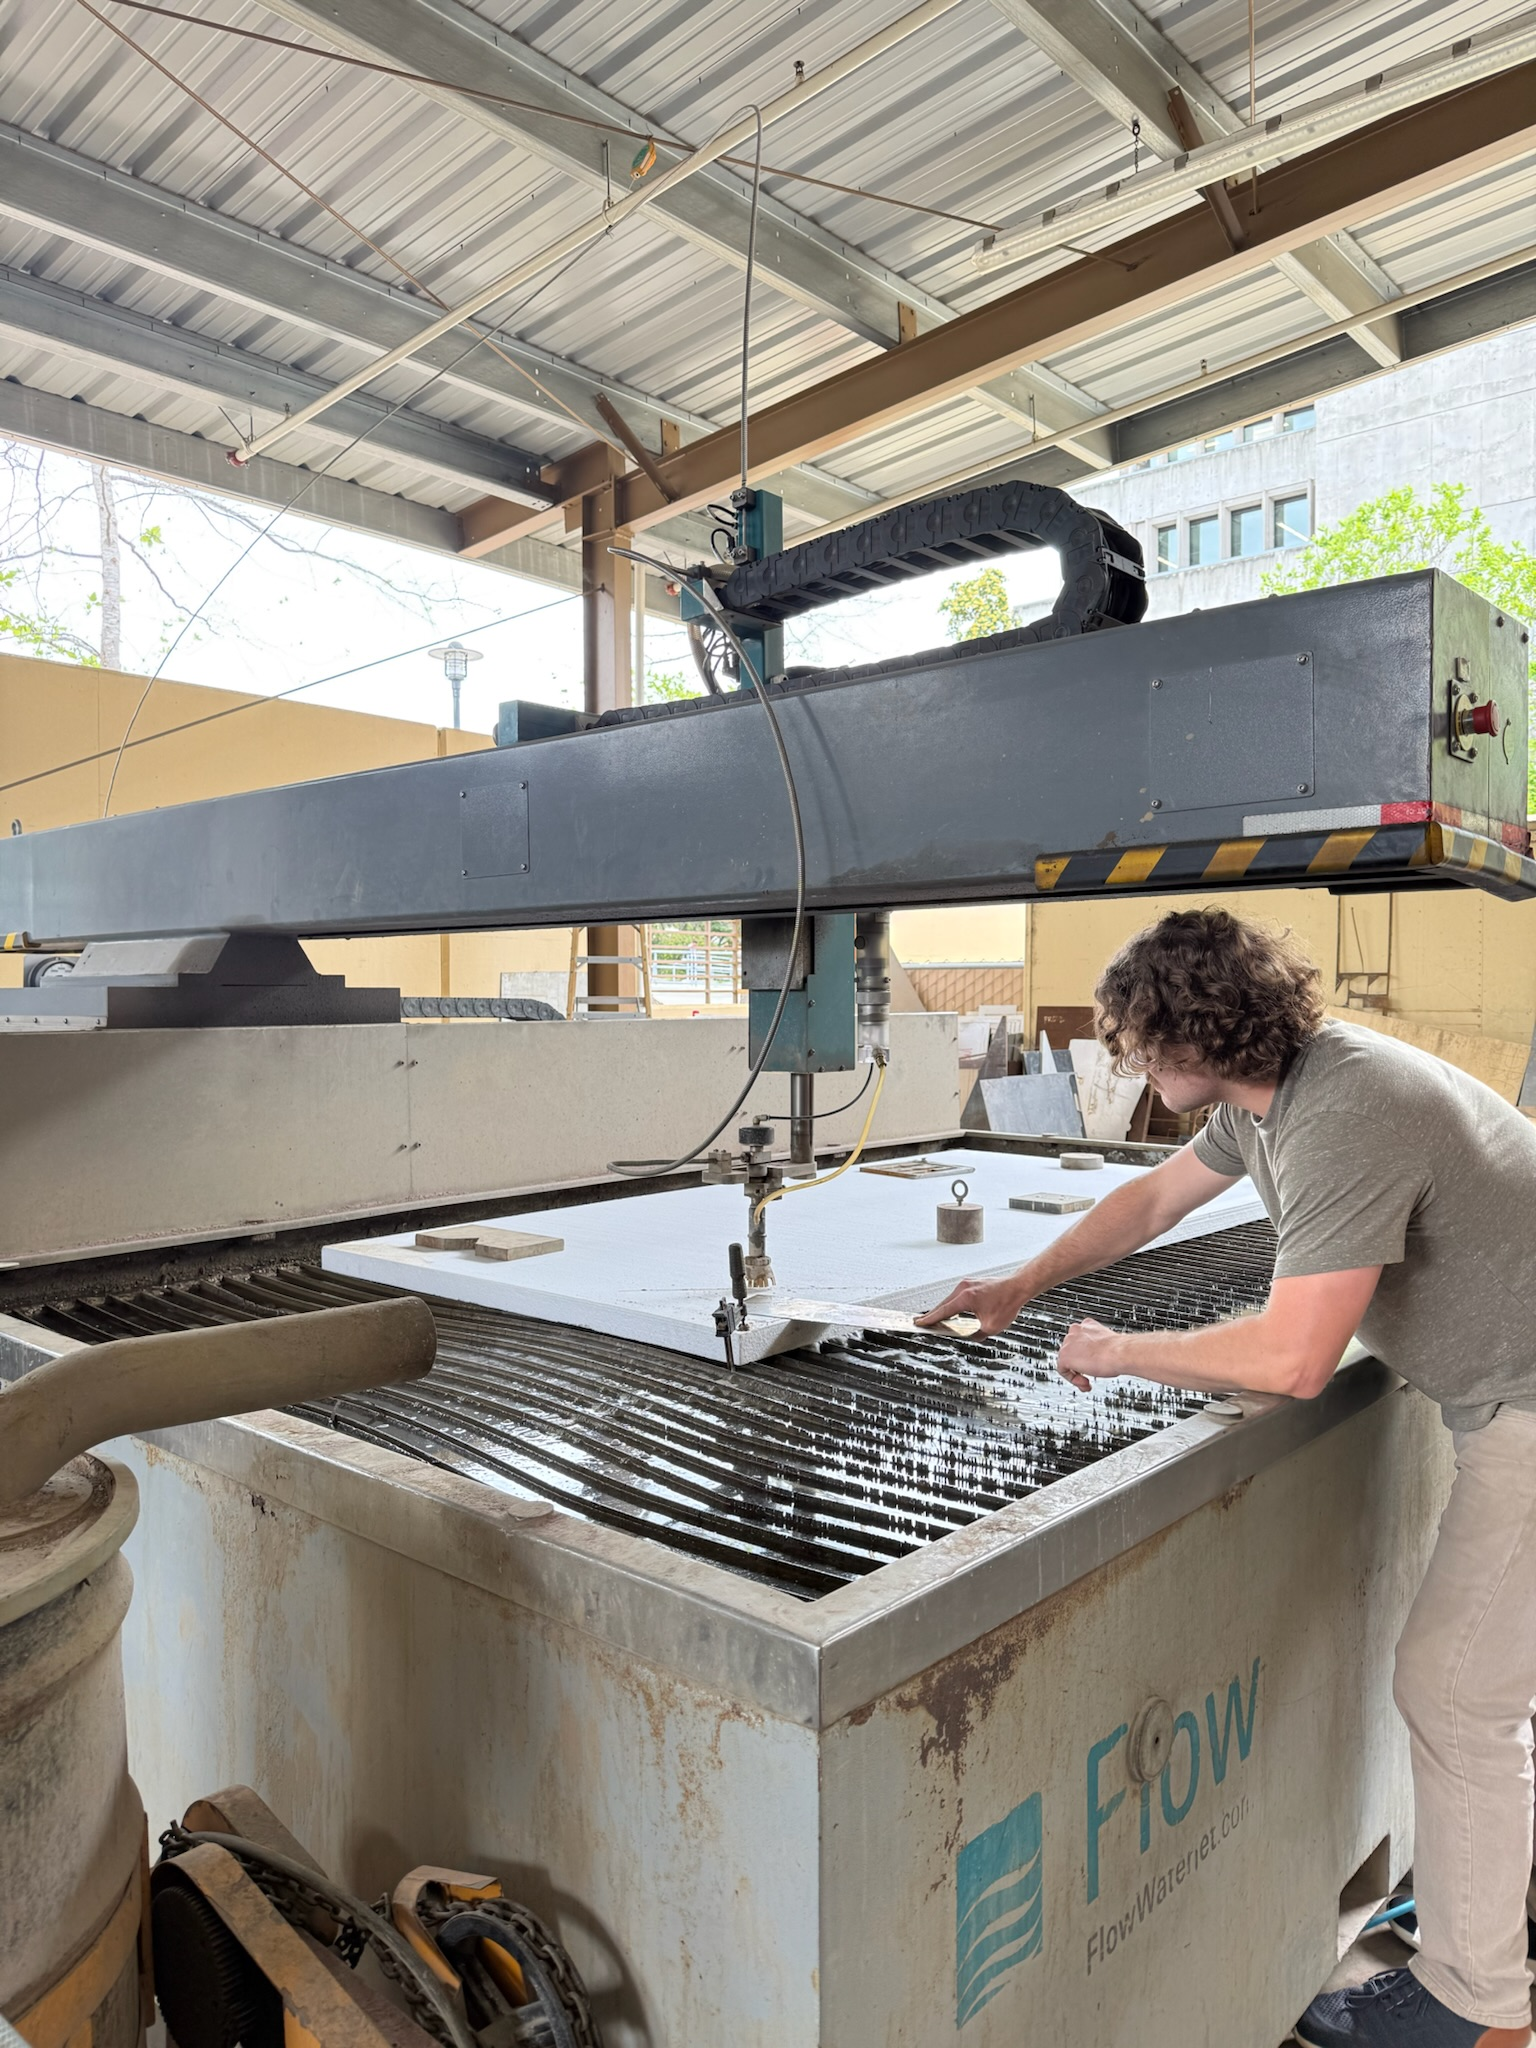
\includegraphics[
        width=3.10in,
        height=1.40in,
        keepaspectratio
    ]{waterjet_foam}
};
\draw[RuleGray,line width=0.55pt,rounded corners=4pt]
    ($(current page.north west)+(0.43in,-3.36in)$)
    rectangle
    ($(current page.north west)+(3.71in,-4.85in)$);

% Row 1 image 2
\node[anchor=center,inner sep=0pt]
at ($(current page.north west)+(5.50in,-4.105in)$)
{
    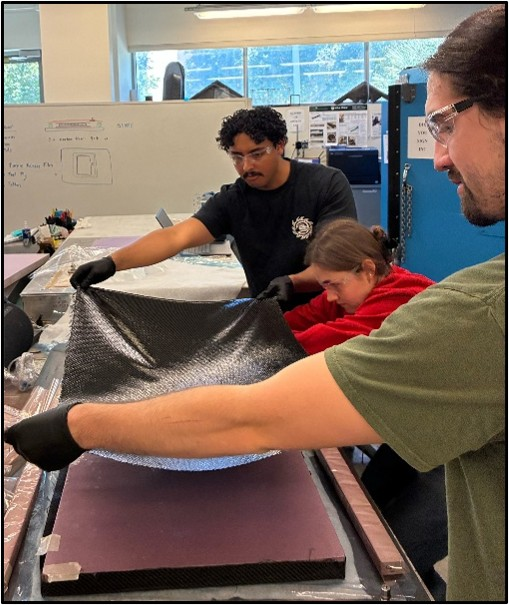
\includegraphics[
        width=3.10in,
        height=1.40in,
        keepaspectratio
    ]{group_layup}
};
\draw[RuleGray,line width=0.55pt,rounded corners=4pt]
    ($(current page.north west)+(3.86in,-3.36in)$)
    rectangle
    ($(current page.north west)+(7.14in,-4.85in)$);

% Row 1 image 3
\node[anchor=center,inner sep=0pt]
at ($(current page.north west)+(8.935in,-4.105in)$)
{
    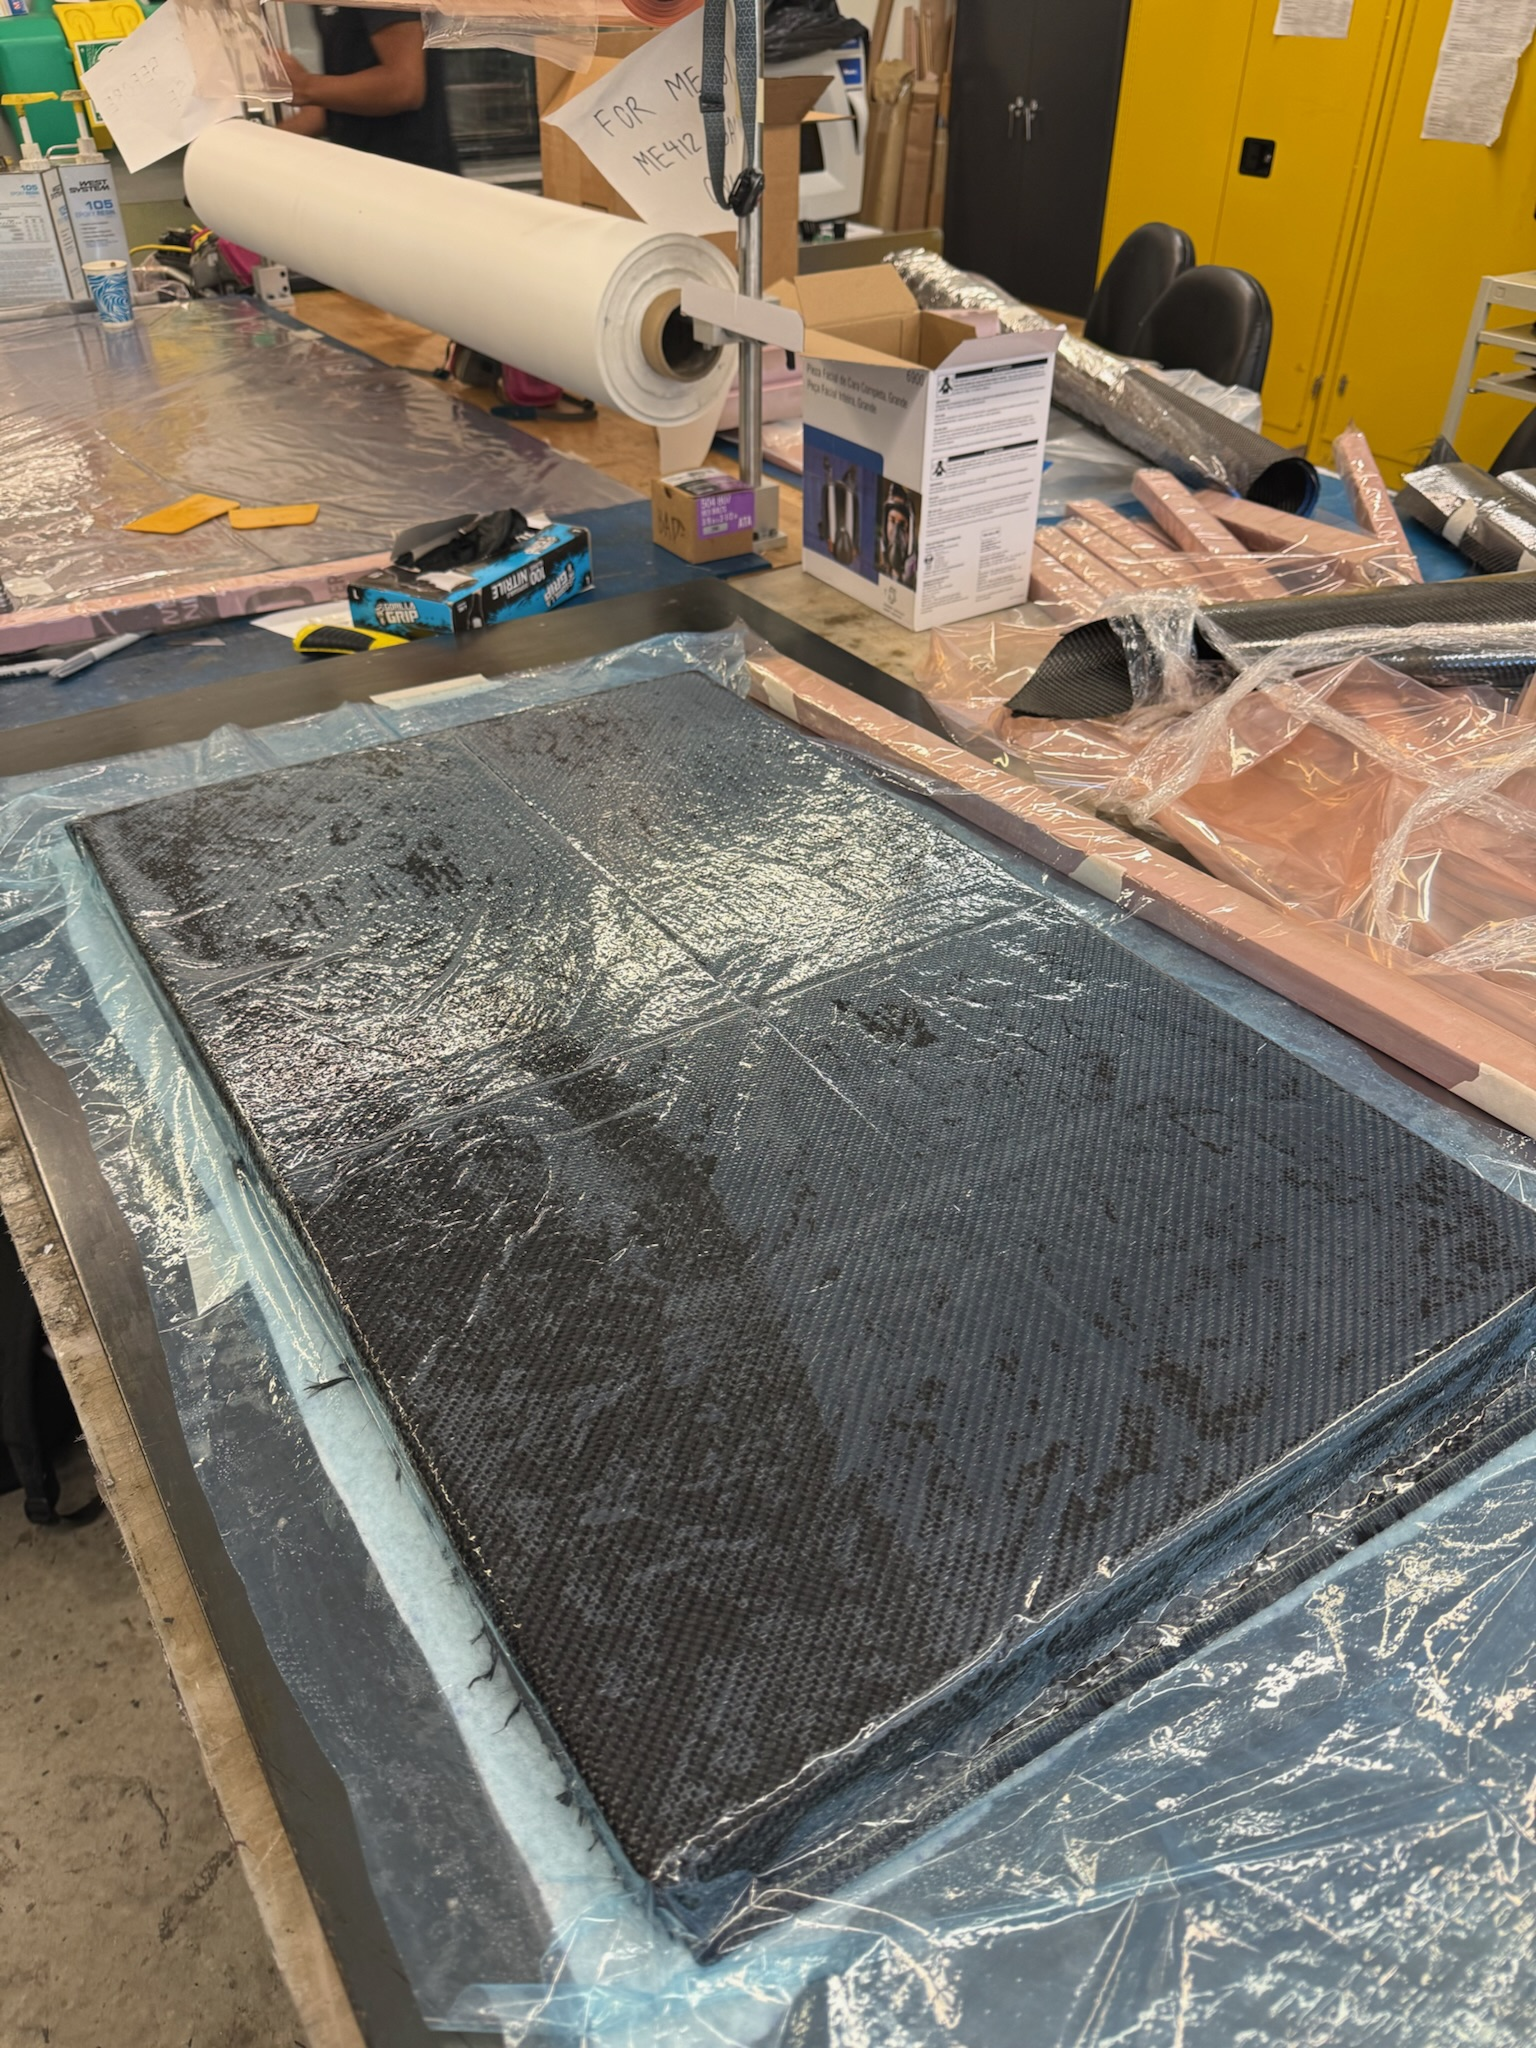
\includegraphics[
        width=3.10in,
        height=1.40in,
        keepaspectratio
    ]{blue_perforrated_film_layup}
};
\draw[RuleGray,line width=0.55pt,rounded corners=4pt]
    ($(current page.north west)+(7.29in,-3.36in)$)
    rectangle
    ($(current page.north east)+(-0.42in,-4.85in)$);

% Row 1 captions
\node[anchor=north,text=Muted,font=\sffamily\fontsize{6.7}{7.3}\selectfont]
at ($(current page.north west)+(2.07in,-4.90in)$)
{1. Waterjet-cut core and perimeter geometry};

\node[anchor=north,text=Muted,font=\sffamily\fontsize{6.7}{7.3}\selectfont]
at ($(current page.north west)+(5.50in,-4.90in)$)
{2. Team wet layup under my process guidance};

\node[anchor=north,text=Muted,font=\sffamily\fontsize{6.7}{7.3}\selectfont]
at ($(current page.north west)+(8.935in,-4.90in)$)
{3. Perforated film, breather, and vacuum enclosure};

% Row 2 image 1
\node[anchor=center,inner sep=0pt]
at ($(current page.north west)+(2.07in,-5.875in)$)
{
    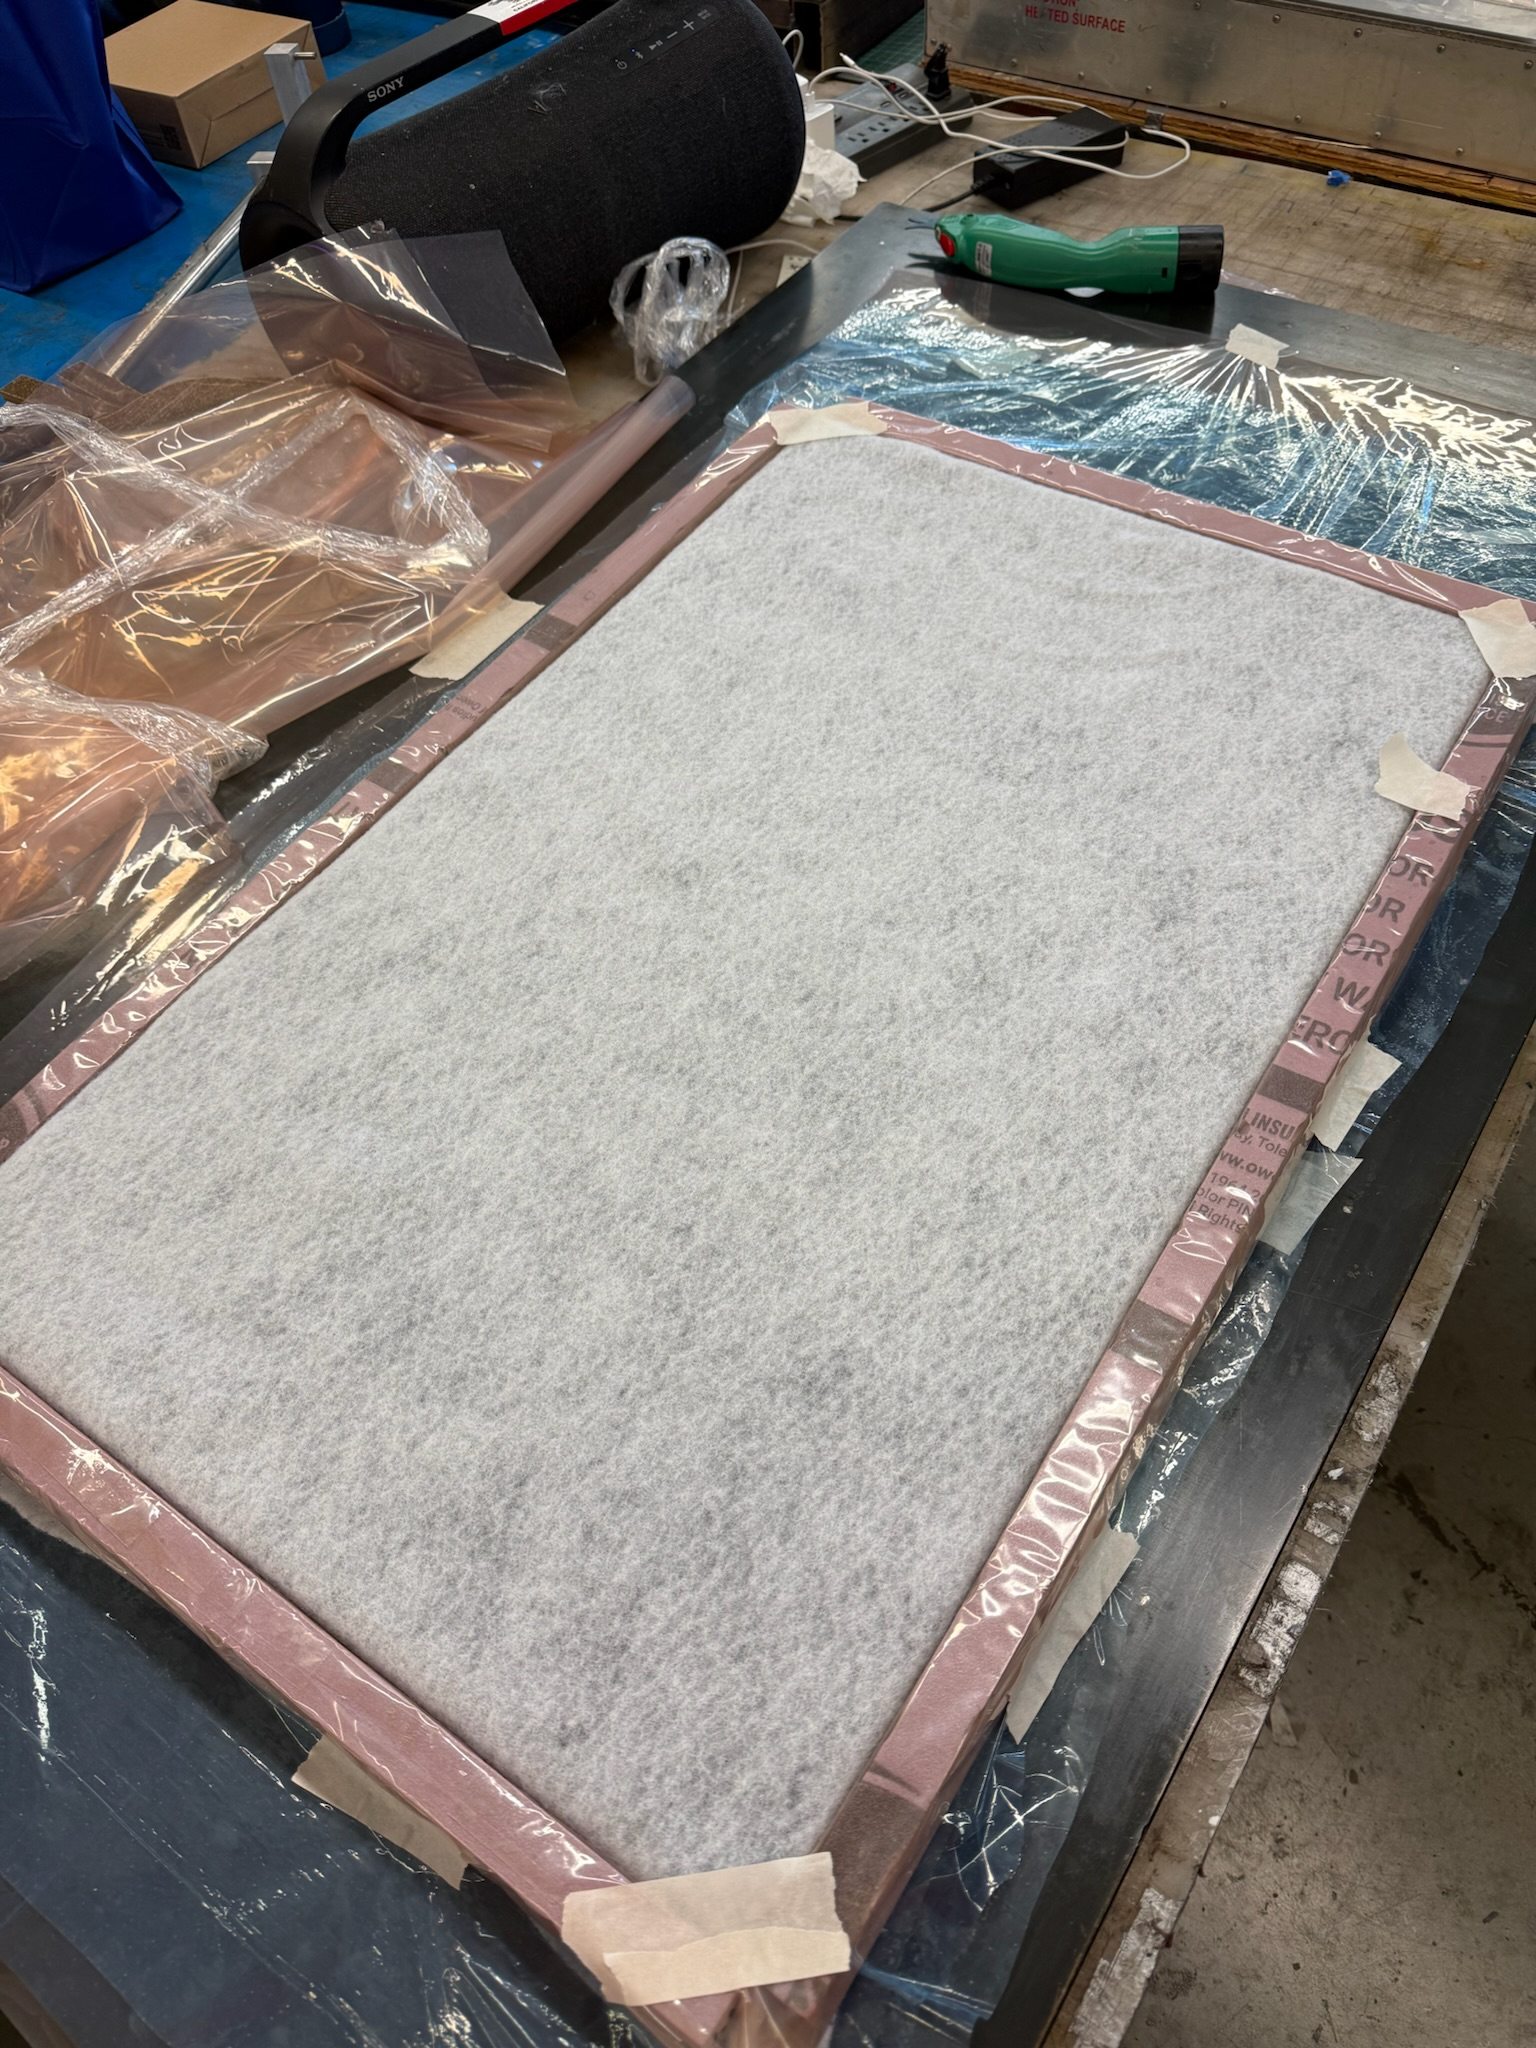
\includegraphics[
        width=3.10in,
        height=1.40in,
        keepaspectratio
    ]{completed_layup}
};
\draw[RuleGray,line width=0.55pt,rounded corners=4pt]
    ($(current page.north west)+(0.43in,-5.13in)$)
    rectangle
    ($(current page.north west)+(3.71in,-6.62in)$);

% Row 2 image 2 — oven chamber used only as a reliable vacuum enclosure; no heat applied
\node[anchor=center,inner sep=0pt]
at ($(current page.north west)+(5.50in,-5.875in)$)
{
    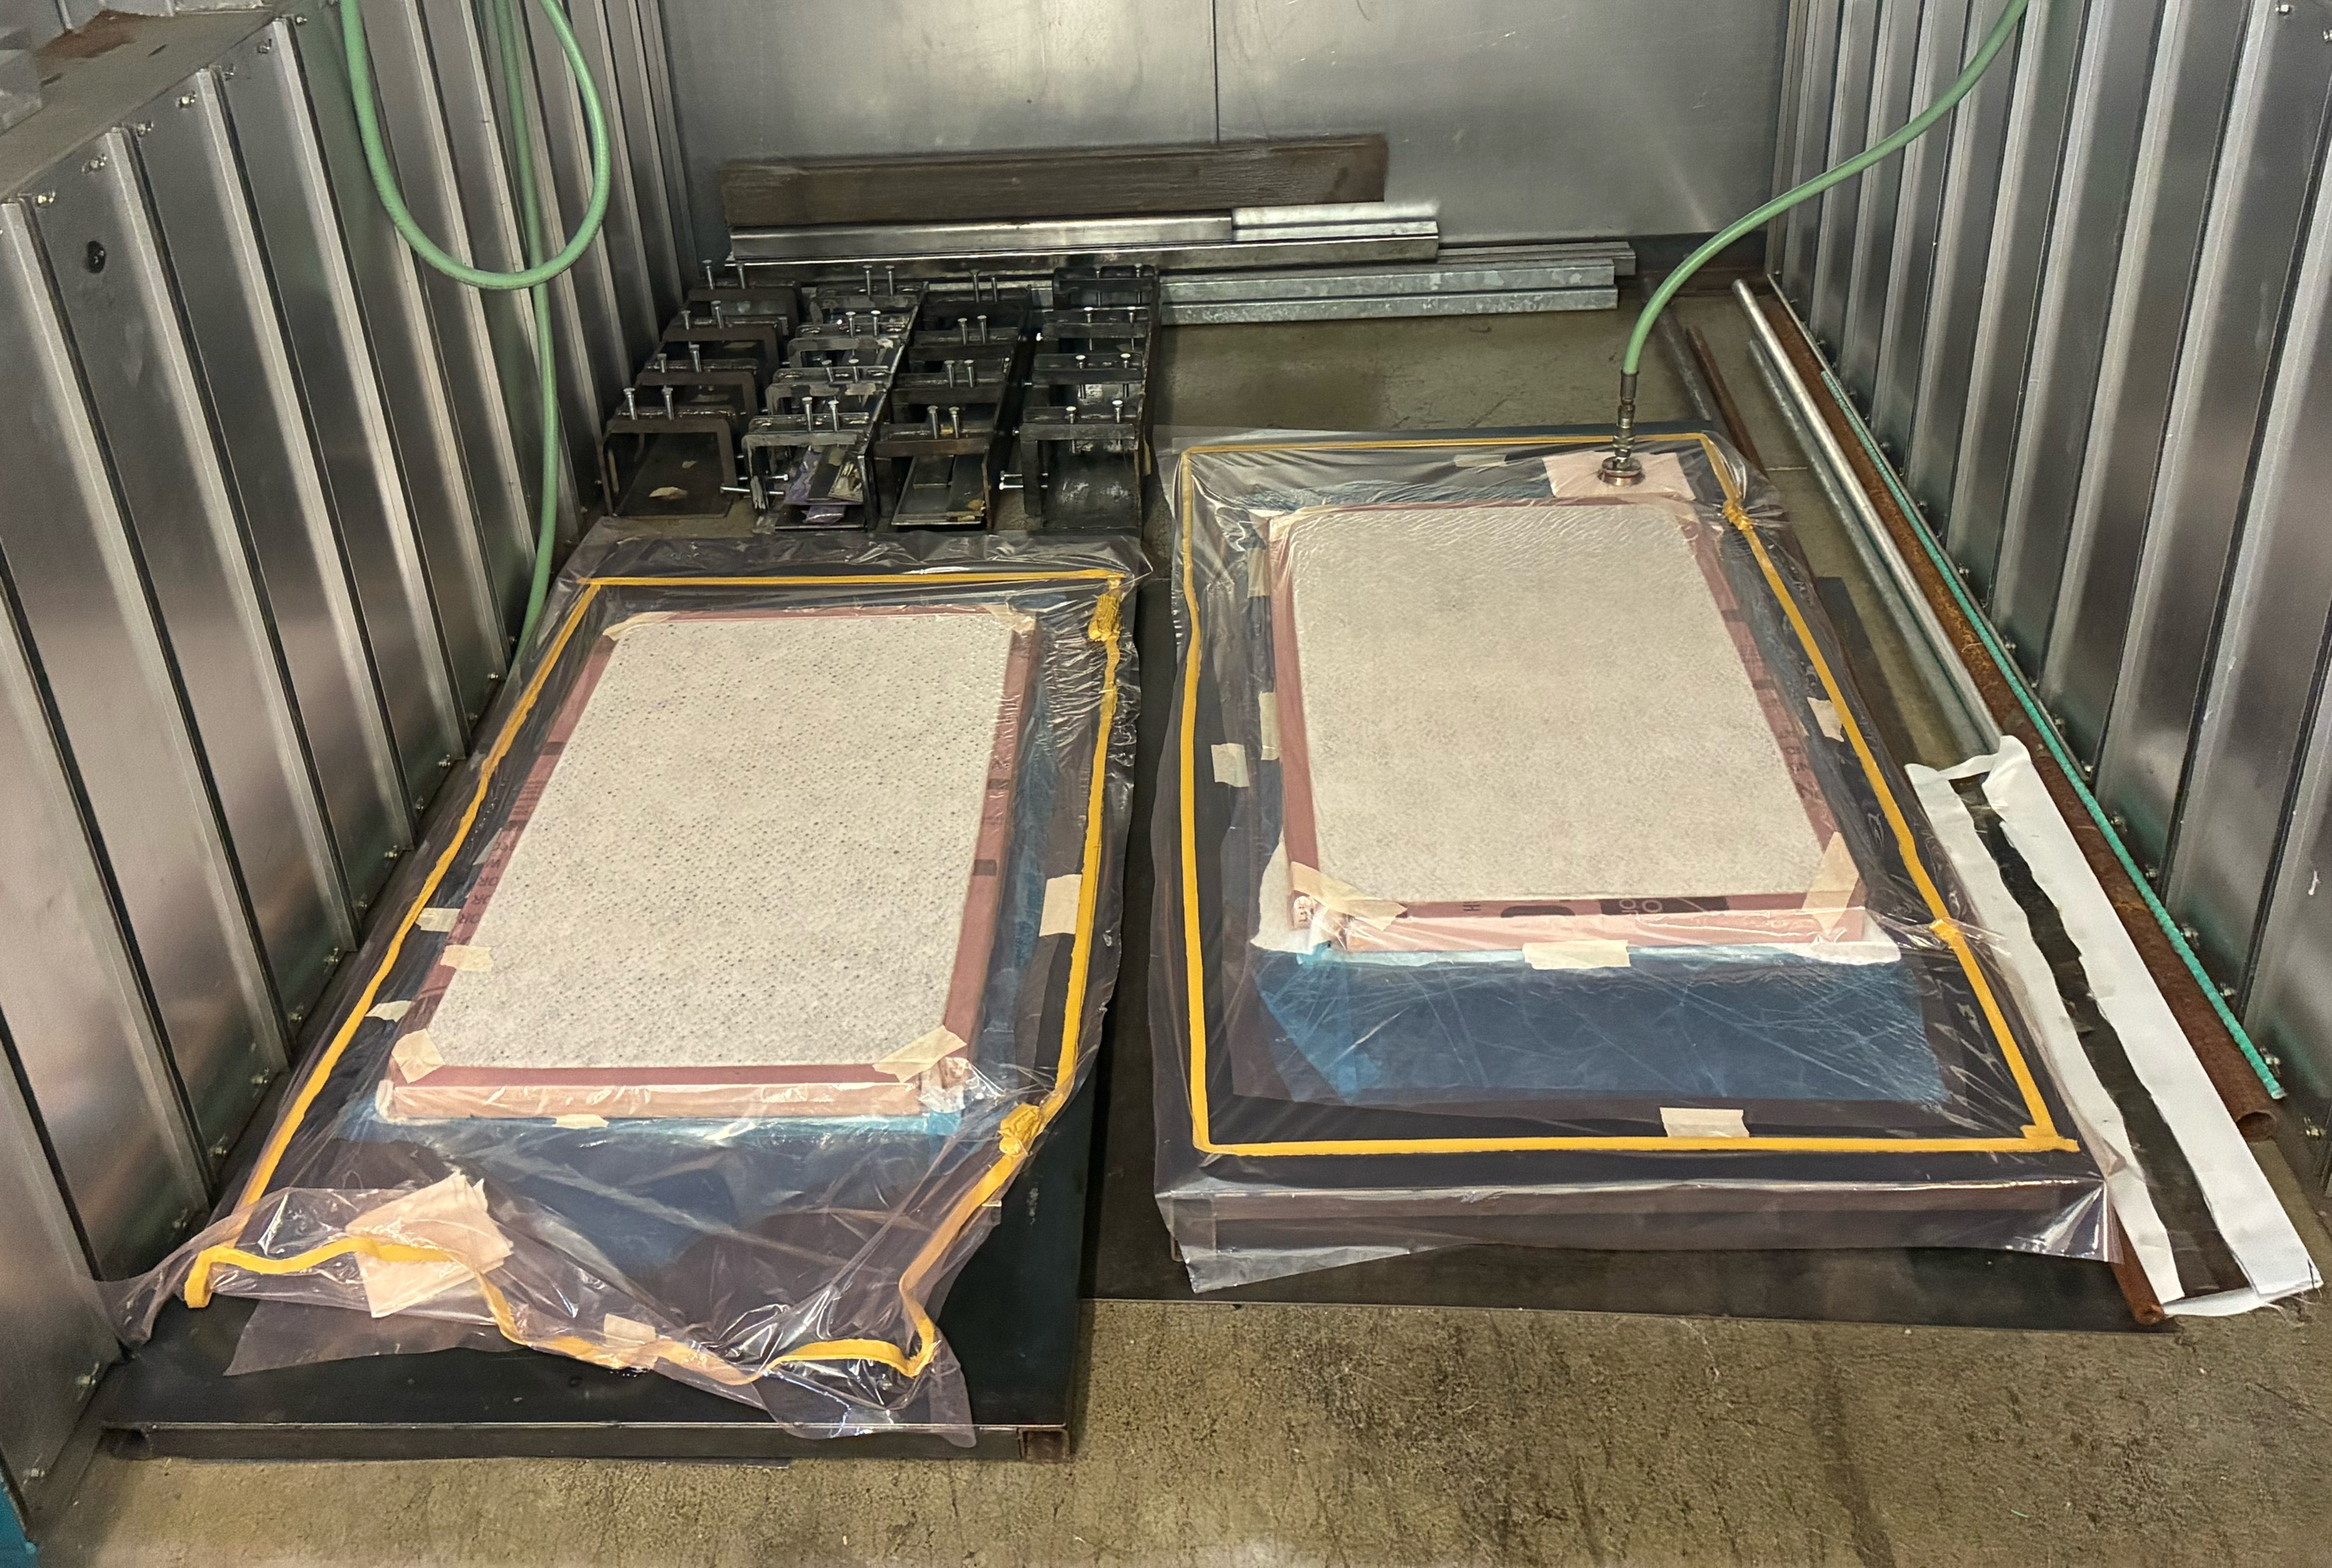
\includegraphics[
        width=3.10in,
        height=1.40in,
        keepaspectratio
    ]{layups_in_composite_oven_under_vacuumPressure}
};
\draw[RuleGray,line width=0.55pt,rounded corners=4pt]
    ($(current page.north west)+(3.86in,-5.13in)$)
    rectangle
    ($(current page.north west)+(7.14in,-6.62in)$);

% Row 2 image 3
\node[anchor=center,inner sep=0pt]
at ($(current page.north west)+(8.935in,-5.875in)$)
{
    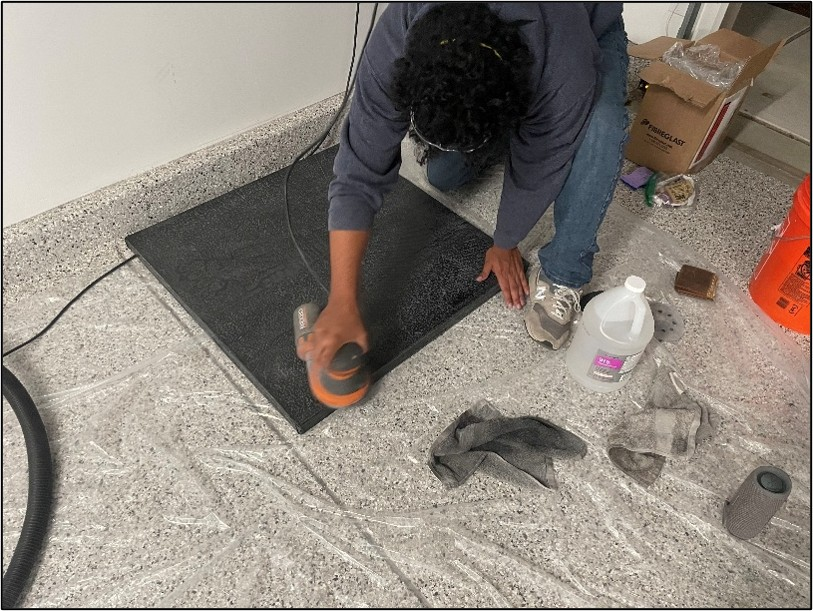
\includegraphics[
        width=3.10in,
        height=1.40in,
        keepaspectratio
    ]{garage_sanding}
};
\draw[RuleGray,line width=0.55pt,rounded corners=4pt]
    ($(current page.north west)+(7.29in,-5.13in)$)
    rectangle
    ($(current page.north east)+(-0.42in,-6.62in)$);

% Row 2 captions
\node[anchor=north,text=Muted,font=\sffamily\fontsize{6.7}{7.3}\selectfont]
at ($(current page.north west)+(2.07in,-6.67in)$)
{4. Fully saturated carbon skin and foam sandwich};

\node[anchor=north,text=Muted,font=\sffamily\fontsize{6.7}{7.3}\selectfont]
at ($(current page.north west)+(5.50in,-6.67in)$)
{5. Room-temperature cure under continuous vacuum};

\node[anchor=north,text=Muted,font=\sffamily\fontsize{6.7}{7.3}\selectfont]
at ($(current page.north west)+(8.935in,-6.67in)$)
{6. Post-processing and surface preparation};

% Bottom callouts
\fill[Panel,rounded corners=4pt]
    ($(current page.north west)+(0.43in,-6.95in)$)
    rectangle
    ($(current page.north west)+(5.48in,-7.60in)$);

\draw[RuleGray,line width=0.55pt,rounded corners=4pt]
    ($(current page.north west)+(0.43in,-6.95in)$)
    rectangle
    ($(current page.north west)+(5.48in,-7.60in)$);

\node[
    anchor=north west,
    text=DeepGreen,
    font=\sffamily\bfseries\fontsize{7.0}{7.6}\selectfont
]
at ($(current page.north west)+(0.63in,-7.08in)$)
{FROM THREE LAYUPS TO ONE};

\node[
    anchor=north west,
    align=left,
    text width=4.56in,
    text=Ink,
    font=\fontsize{6.45}{7.45}\selectfont
]
at ($(current page.north west)+(0.63in,-7.29in)$)
{
The Envelope Method reduced labor, cure cycles, handling,
alignment risk, and time spent forming numerous vacuum-bag
pleats around the 1.5-inch-thick XPS panels.
};

\fill[Panel,rounded corners=4pt]
    ($(current page.north west)+(5.68in,-6.95in)$)
    rectangle
    ($(current page.north east)+(-0.42in,-7.60in)$);

\draw[RuleGray,line width=0.55pt,rounded corners=4pt]
    ($(current page.north west)+(5.68in,-6.95in)$)
    rectangle
    ($(current page.north east)+(-0.42in,-7.60in)$);

\node[
    anchor=north west,
    text=DeepGreen,
    font=\sffamily\bfseries\fontsize{7.0}{7.6}\selectfont
]
at ($(current page.north west)+(5.88in,-7.08in)$)
{WHY SURFACE-BONDED HARDWARE};

\node[
    anchor=north west,
    align=left,
    text width=4.55in,
    text=Ink,
    font=\fontsize{6.45}{7.45}\selectfont
]
at ($(current page.north west)+(5.88in,-7.29in)$)
{
Adhesively bonded hinges and fixtures preserved the clean
composite exterior and avoided drilled inserts, foam-core
crushing, added stress concentrations, and new leak paths.
};


% Footer
\node[
    anchor=south west,
    text=white,
    font=\sffamily\bfseries\fontsize{7.1}{7.7}\selectfont
]
at ($(current page.south west)+(0.42in,0.17in)$)
{\faArrowLeft\ PRODUCT ARCHITECTURE};

\node[
    anchor=south,
    text=white,
    font=\sffamily\fontsize{7.0}{7.6}\selectfont
]
at ($(current page.south)+(0,0.17in)$)
{TORO COVER \hspace{6pt} 2 / 3};

\node[
    anchor=south east,
    text=white,
    font=\sffamily\bfseries\fontsize{7.1}{7.7}\selectfont
]
at ($(current page.south east)+(-0.42in,0.17in)$)
{VALIDATION \& TAKEAWAYS \faArrowRight};

\end{tikzpicture}


% ============================================================
% PAGE 3 — FINISHING, VALIDATION, AND TAKEAWAYS
% ============================================================

\clearpage
\thispagestyle{empty}
\hypertarget{toro-results}{}
\null

\begin{tikzpicture}[remember picture,overlay]

% Background and bars
\fill[white]
    (current page.south west)
    rectangle
    (current page.north east);

\fill[DeepGreen]
    (current page.north west)
    rectangle
    ($(current page.north east)+(0,-0.095in)$);

\fill[PolyGold]
    ($(current page.north west)+(0,-0.095in)$)
    rectangle
    ($(current page.north east)+(0,-0.14in)$);

\fill[DeepGreen]
    (current page.south west)
    rectangle
    ($(current page.south east)+(0,0.36in)$);

\fill[PolyGold]
    ($(current page.south west)+(0,0.36in)$)
    rectangle
    ($(current page.south east)+(0,0.405in)$);

% Header
\node[
    anchor=north west,
    text=PolyGold,
    font=\sffamily\bfseries\fontsize{8.1}{8.7}\selectfont
]
at ($(current page.north west)+(0.42in,-0.39in)$)
{TORO COVER \hspace{5pt}/\hspace{5pt} VALIDATION AND ENGINEERING TAKEAWAYS};

\node[
    anchor=north west,
    text=DeepGreen,
    font=\bfseries\fontsize{22.5}{23.5}\selectfont
]
at ($(current page.north west)+(0.40in,-0.67in)$)
{FROM PROTOTYPE TO PRODUCT PATHWAY};

\node[
    anchor=north west,
    text=Muted,
    font=\sffamily\fontsize{8.7}{9.6}\selectfont
]
at ($(current page.north west)+(0.42in,-1.12in)$)
{Environmental protection, usability testing, scope decisions, and lessons from technical leadership};

\fill[PolyGold]
    ($(current page.north west)+(0.42in,-1.36in)$)
    rectangle
    ($(current page.north west)+(5.8in,-1.315in)$);

% Finishing title
\node[
    anchor=north west,
    text=DeepGreen,
    font=\sffamily\bfseries\fontsize{8.0}{8.7}\selectfont
]
at ($(current page.north west)+(0.43in,-1.62in)$)
{OUTDOOR FINISHING AND ENVIRONMENTAL PROTECTION};

% Image 1
\node[anchor=center,inner sep=0pt]
at ($(current page.north west)+(1.705in,-2.655in)$)
{
    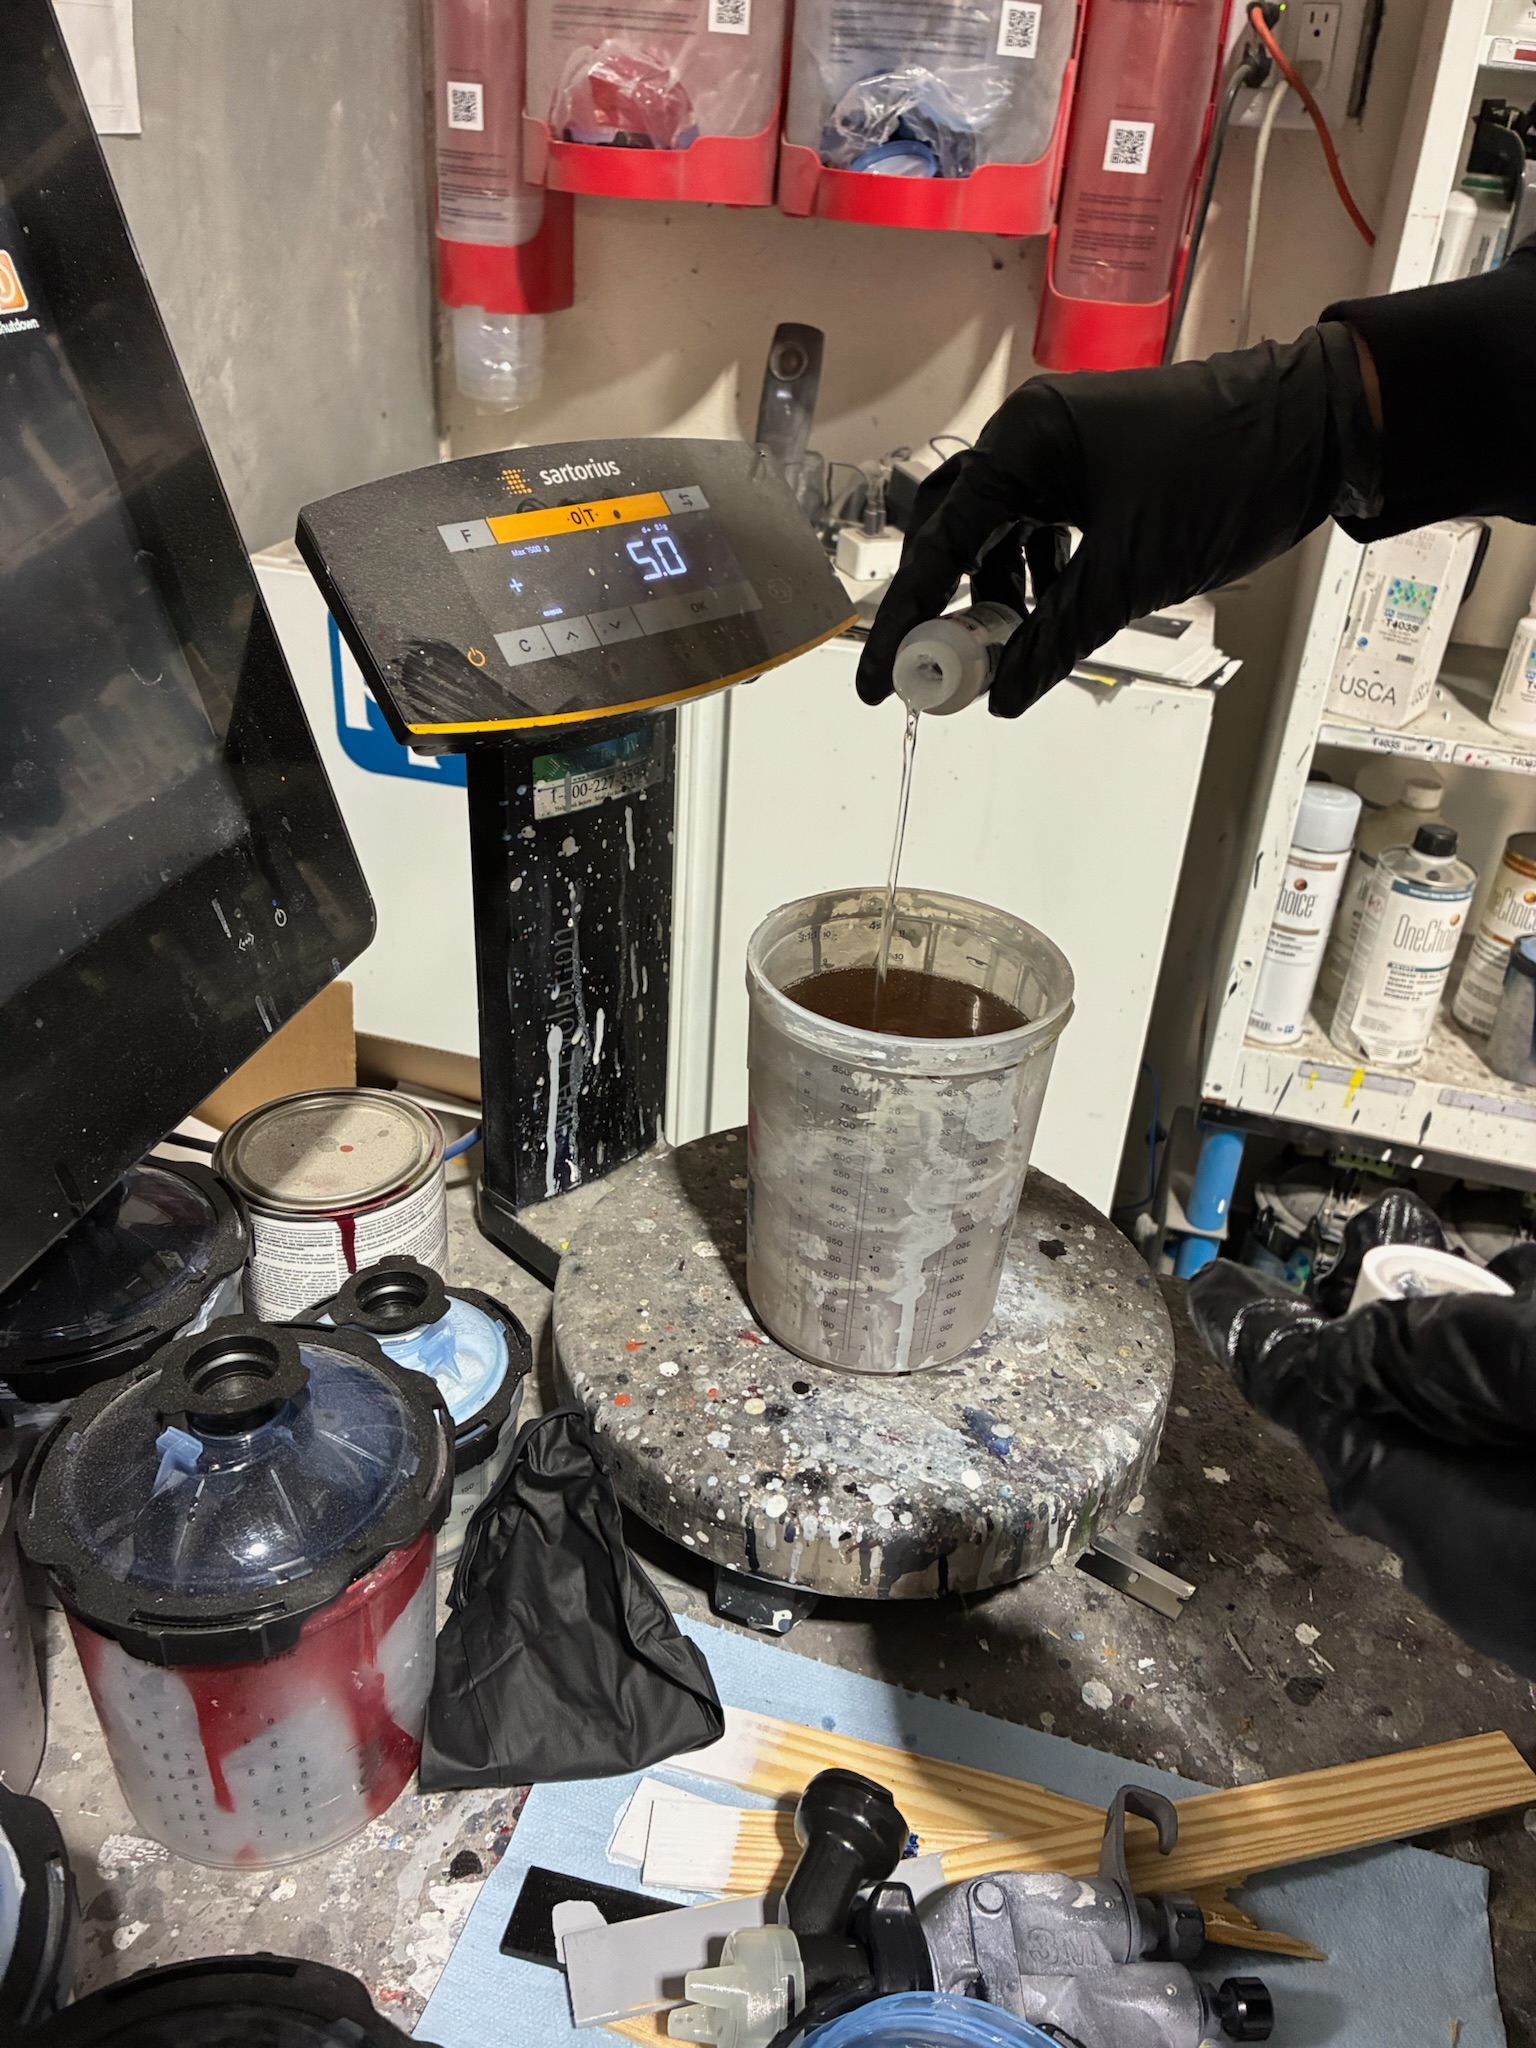
\includegraphics[
        width=2.35in,
        height=1.40in,
        keepaspectratio
    ]{spray_topcoat_prep}
};
\draw[RuleGray,line width=0.55pt,rounded corners=4pt]
    ($(current page.north west)+(0.43in,-1.91in)$)
    rectangle
    ($(current page.north west)+(2.98in,-3.40in)$);

% Image 2
\node[anchor=center,inner sep=0pt]
at ($(current page.north west)+(4.375in,-2.655in)$)
{
    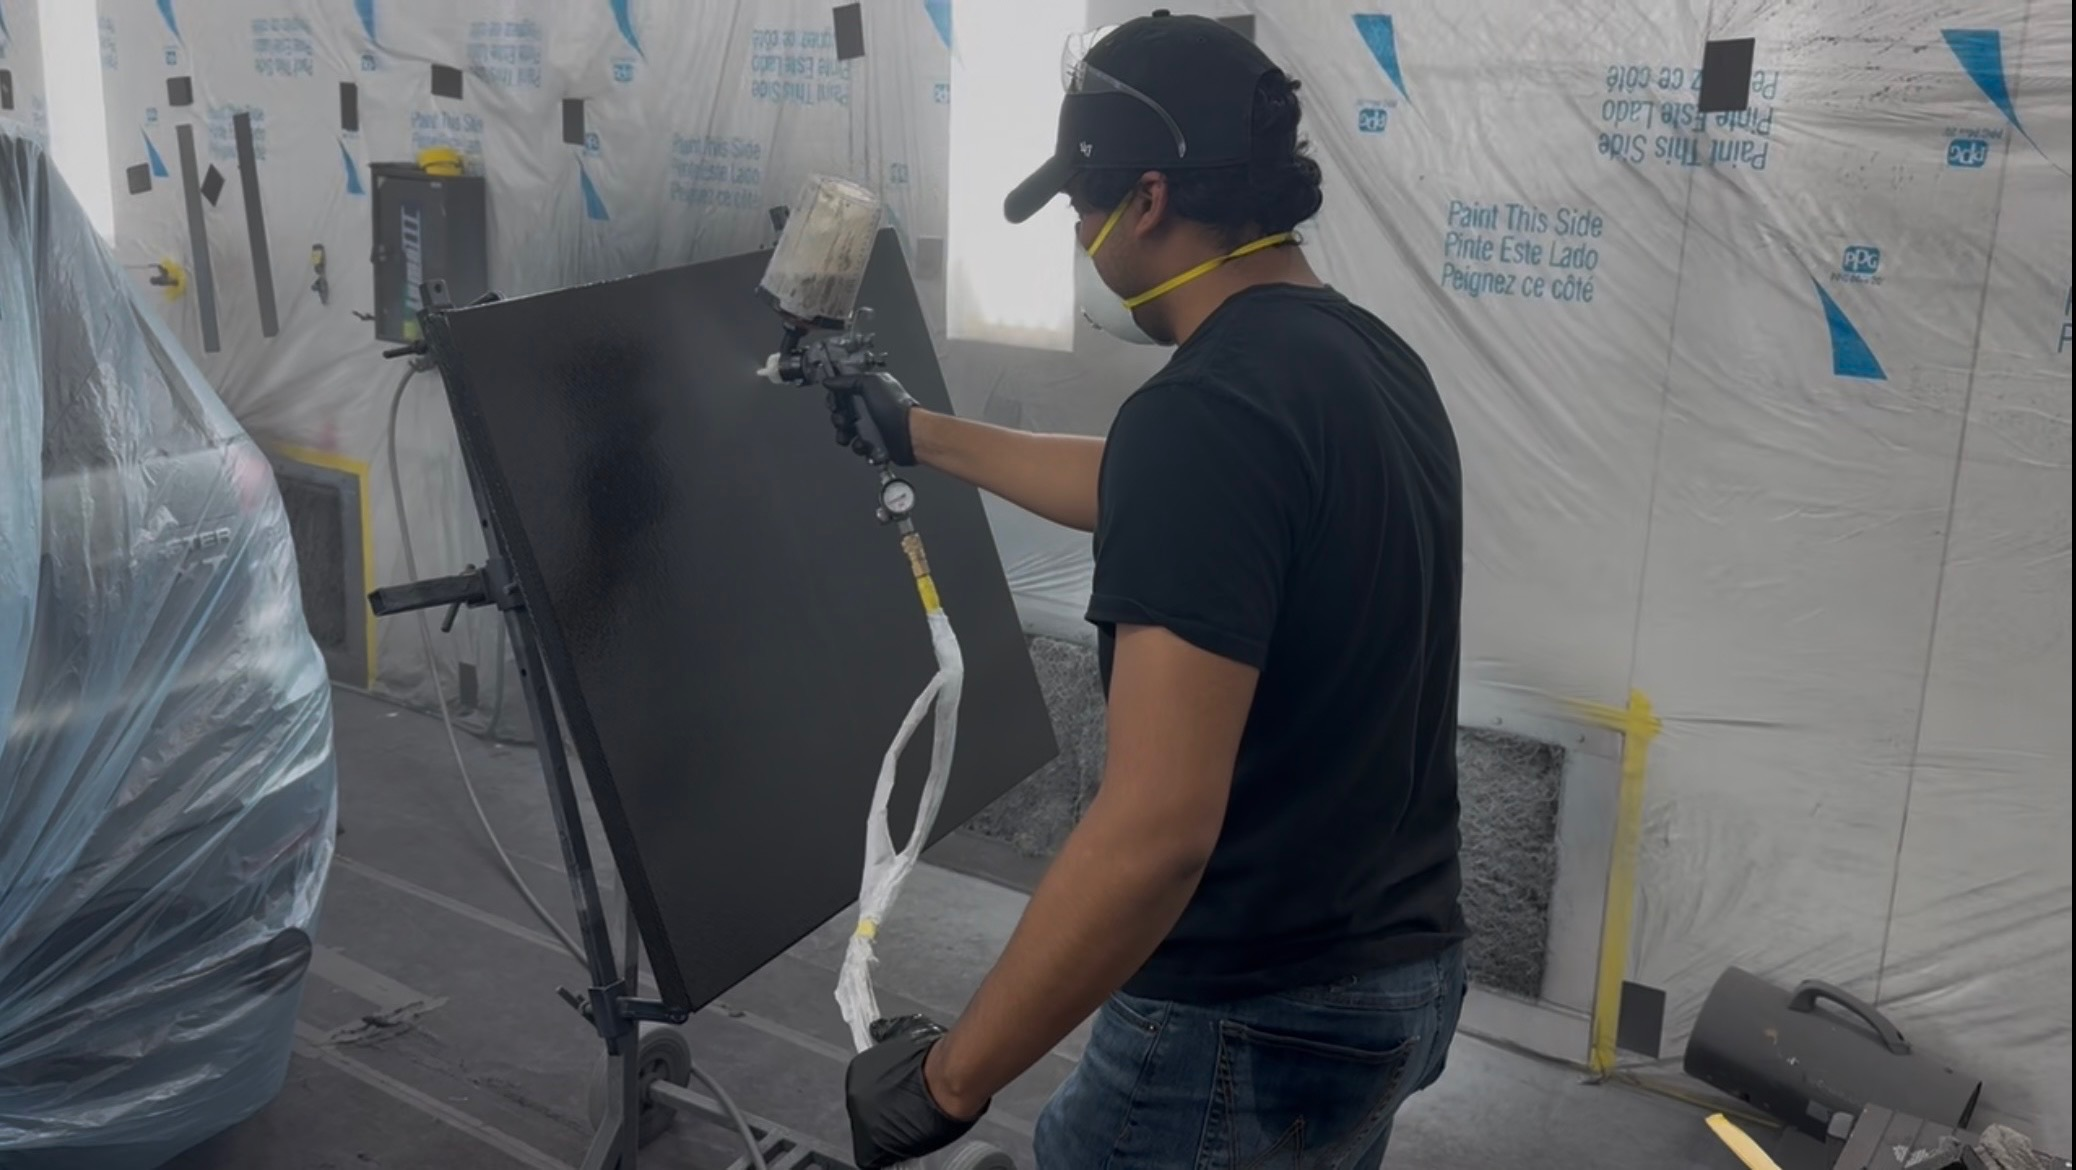
\includegraphics[
        width=2.35in,
        height=1.40in,
        keepaspectratio
    ]{spraying_topcoat}
};
\draw[RuleGray,line width=0.55pt,rounded corners=4pt]
    ($(current page.north west)+(3.10in,-1.91in)$)
    rectangle
    ($(current page.north west)+(5.65in,-3.40in)$);

% Image 3
\node[anchor=center,inner sep=0pt]
at ($(current page.north west)+(7.045in,-2.655in)$)
{
    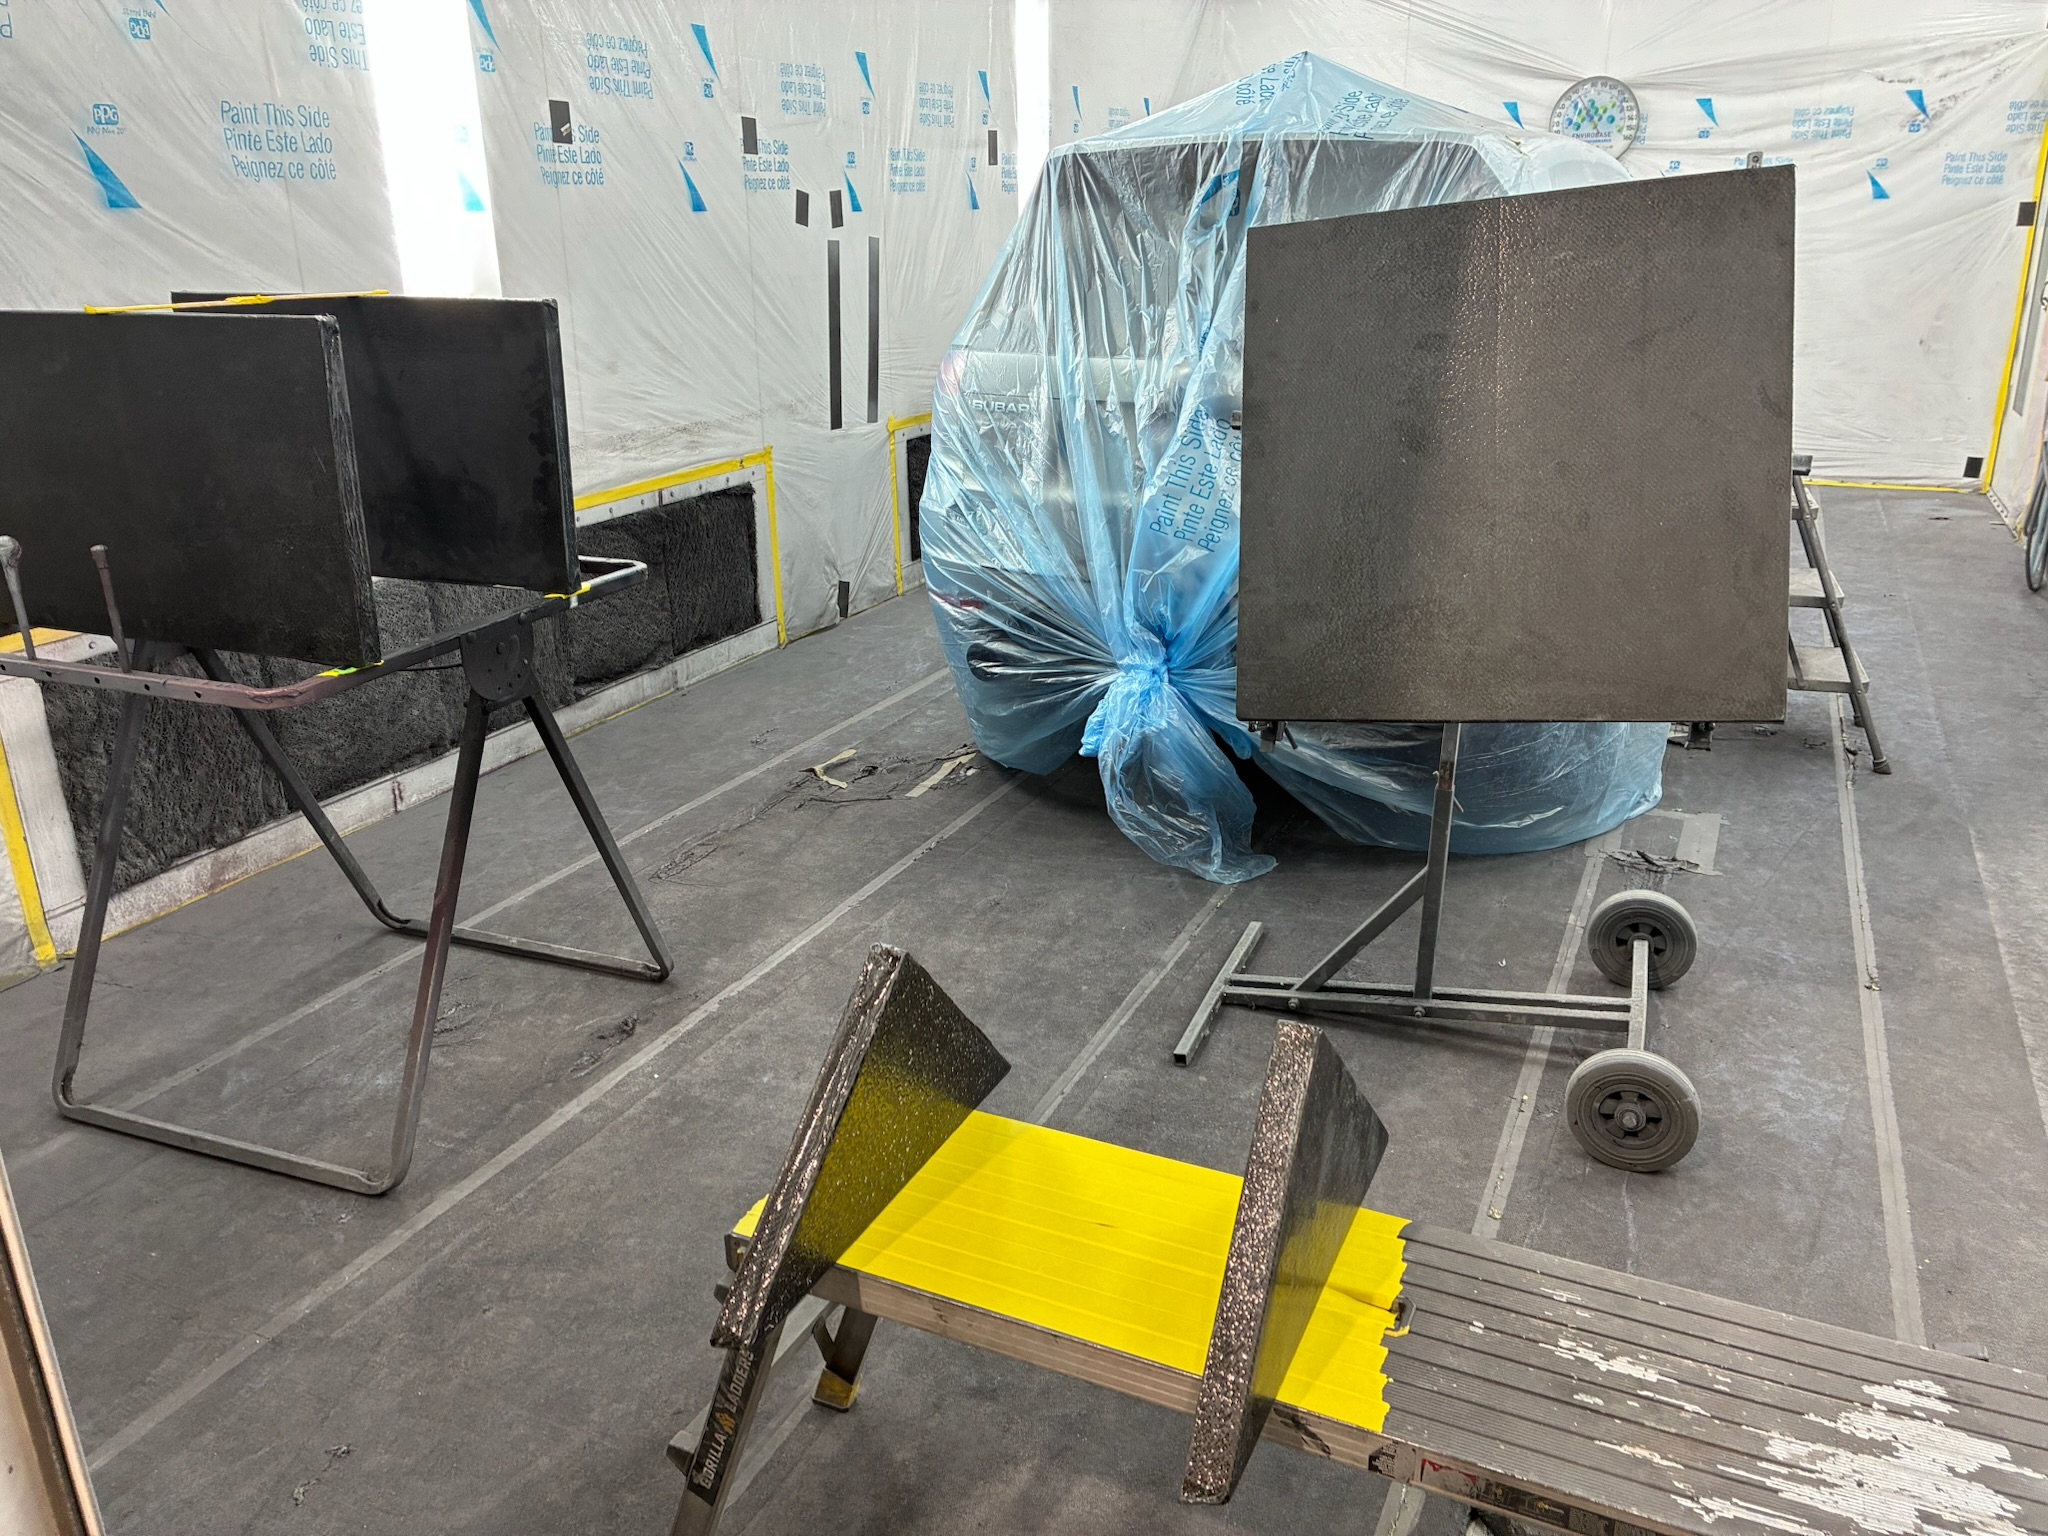
\includegraphics[
        width=2.35in,
        height=1.40in,
        keepaspectratio
    ]{topcoat_setup_apparatus}
};
\draw[RuleGray,line width=0.55pt,rounded corners=4pt]
    ($(current page.north west)+(5.77in,-1.91in)$)
    rectangle
    ($(current page.north west)+(8.32in,-3.40in)$);

% Image 4
\node[anchor=center,inner sep=0pt]
at ($(current page.north west)+(9.50in,-2.655in)$)
{
    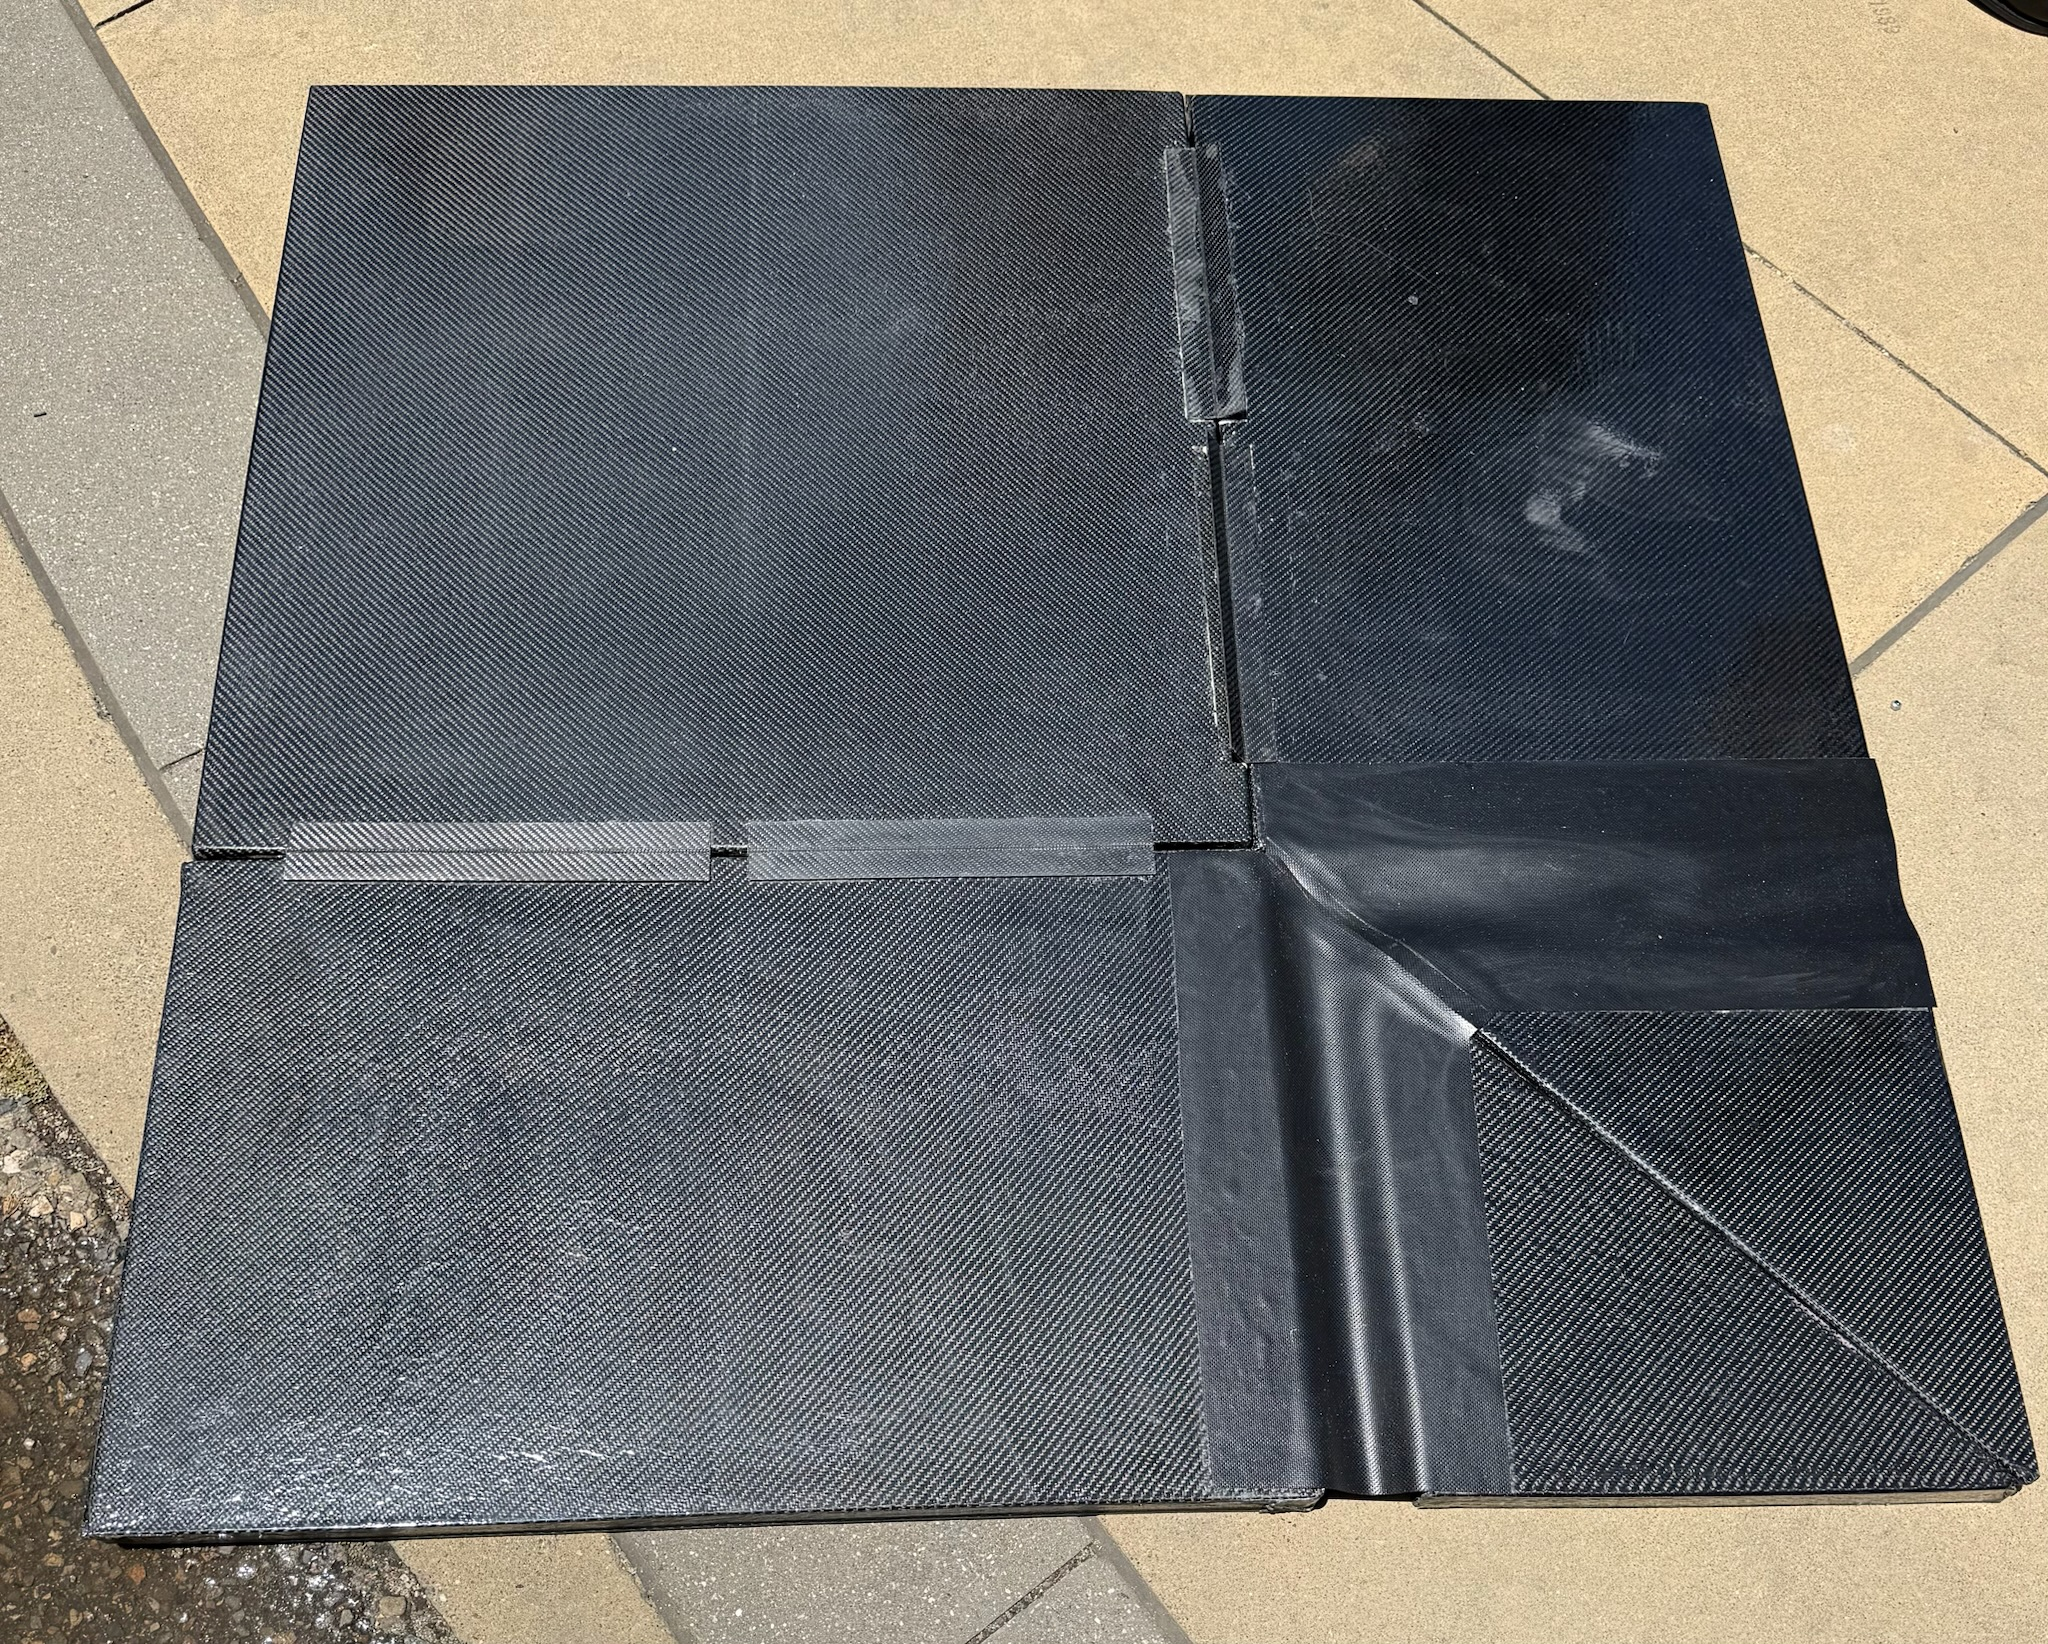
\includegraphics[
        width=2.35in,
        height=1.40in,
        keepaspectratio
    ]{refined_final_toro_cover_partial_carbon_model}
};
\draw[RuleGray,line width=0.55pt,rounded corners=4pt]
    ($(current page.north west)+(8.44in,-1.91in)$)
    rectangle
    ($(current page.north east)+(-0.42in,-3.40in)$);

% Captions
\node[anchor=north,text=Muted,font=\sffamily\fontsize{6.7}{7.3}\selectfont]
at ($(current page.north west)+(1.705in,-3.45in)$)
{Topcoat material preparation};

\node[anchor=north,text=Muted,font=\sffamily\fontsize{6.7}{7.3}\selectfont]
at ($(current page.north west)+(4.375in,-3.45in)$)
{Automotive-booth topcoat application};

\node[anchor=north,text=Muted,font=\sffamily\fontsize{6.7}{7.3}\selectfont]
at ($(current page.north west)+(7.045in,-3.45in)$)
{Coated panels drying after application};

\node[anchor=north,text=Muted,font=\sffamily\fontsize{6.7}{7.3}\selectfont]
at ($(current page.north west)+(9.50in,-3.45in)$)
{Partial carbon manufacturing model};

% Environmental rationale
\fill[SoftGold,rounded corners=4pt]
    ($(current page.north west)+(0.43in,-3.73in)$)
    rectangle
    ($(current page.north east)+(-0.42in,-4.76in)$);

\node[
    anchor=north west,
    align=left,
    text width=9.75in,
    text=Ink,
    font=\fontsize{7.05}{8.25}\selectfont
]
at ($(current page.north west)+(0.65in,-3.89in)$)
{
Because the sponsor required a carbon-fiber cover for outdoor use near chlorinated water,
environmental protection became a functional requirement rather than a cosmetic finish.
I selected and personally sprayed a UV-resistant Sunshield topcoat to seal minor laminate
porosity, reduce moisture ingress, preserve the carbon appearance, limit UV degradation of
the epoxy matrix, and isolate the composite surface from nearby metallic hardware.
};

% Results title
\node[
    anchor=north west,
    text=DeepGreen,
    font=\sffamily\bfseries\fontsize{8.0}{8.7}\selectfont
]
at ($(current page.north west)+(0.43in,-4.94in)$)
{FUNCTIONAL PROTOTYPE RESULTS};

% ------------------------------------------------------------
% Matched lower panels — larger type and improved allocation
% ------------------------------------------------------------

% Left results panel
\fill[SoftGreen,rounded corners=5pt]
    ($(current page.north west)+(0.43in,-5.22in)$)
    rectangle
    ($(current page.north west)+(5.98in,-7.39in)$);

\draw[RuleGray,line width=0.65pt,rounded corners=5pt]
    ($(current page.north west)+(0.43in,-5.22in)$)
    rectangle
    ($(current page.north west)+(5.98in,-7.39in)$);

\fill[DeepGreen,rounded corners=5pt]
    ($(current page.north west)+(0.43in,-5.22in)$)
    rectangle
    ($(current page.north west)+(5.98in,-5.58in)$);

\fill[DeepGreen]
    ($(current page.north west)+(0.43in,-5.40in)$)
    rectangle
    ($(current page.north west)+(5.98in,-5.58in)$);

\node[anchor=west,text=white,
      font=\sffamily\bfseries\fontsize{7.0}{7.6}\selectfont]
at ($(current page.north west)+(0.66in,-5.40in)$)
{SPECIFICATION};

\node[anchor=west,text=white,
      font=\sffamily\bfseries\fontsize{7.0}{7.6}\selectfont]
at ($(current page.north west)+(3.02in,-5.40in)$)
{RESULT};

\node[anchor=east,text=white,
      font=\sffamily\bfseries\fontsize{7.0}{7.6}\selectfont]
at ($(current page.north west)+(5.55in,-5.40in)$)
{STATUS};

\node[
    anchor=north west,
    align=left,
    text width=2.15in,
    text=Ink,
    font=\bfseries\fontsize{7.15}{8.55}\selectfont
]
at ($(current page.north west)+(0.66in,-5.72in)$)
{
Deployment time\\[3.4pt]
Removal time\\[3.4pt]
Single-user operation\\[3.4pt]
Single-side operation\\[3.4pt]
Deployment steps\\[3.4pt]
Removal steps\\[3.4pt]
Weight\\[3.4pt]
Folded storage
};

\node[
    anchor=north west,
    align=left,
    text width=1.45in,
    text=Ink,
    font=\fontsize{7.15}{8.55}\selectfont
]
at ($(current page.north west)+(3.02in,-5.72in)$)
{
25.51 seconds\\[3.4pt]
37.22 seconds\\[3.4pt]
100\% successful\\[3.4pt]
75\% successful\\[3.4pt]
6.4 average\\[3.4pt]
9 average\\[3.4pt]
17 lb\\[3.4pt]
2.9' x 2.9' x 1.7'
};

\node[
    anchor=north east,
    align=right,
    text width=1.05in,
    text=DeepGreen,
    font=\sffamily\bfseries\fontsize{7.05}{8.55}\selectfont
]
at ($(current page.north west)+(5.55in,-5.72in)$)
{
PASS\\[3.4pt]
PASS\\[3.4pt]
PASS\\[3.4pt]
NEAR TARGET\\[3.4pt]
PASS\\[3.4pt]
PASS\\[3.4pt]
NEAR TARGET\\[3.4pt]
PASS
};

% Right takeaways panel — widened for easier reading
\fill[SoftGreen,rounded corners=5pt]
    ($(current page.north west)+(6.14in,-5.22in)$)
    rectangle
    ($(current page.north east)+(-0.42in,-7.39in)$);

\draw[RuleGray,line width=0.65pt,rounded corners=5pt]
    ($(current page.north west)+(6.14in,-5.22in)$)
    rectangle
    ($(current page.north east)+(-0.42in,-7.39in)$);

\fill[DeepGreen,rounded corners=5pt]
    ($(current page.north west)+(6.14in,-5.22in)$)
    rectangle
    ($(current page.north east)+(-0.42in,-5.58in)$);

\fill[DeepGreen]
    ($(current page.north west)+(6.14in,-5.40in)$)
    rectangle
    ($(current page.north east)+(-0.42in,-5.58in)$);

\node[anchor=west,text=white,
      font=\sffamily\bfseries\fontsize{7.1}{7.7}\selectfont]
at ($(current page.north west)+(6.38in,-5.40in)$)
{ENGINEERING TAKEAWAYS};

\node[
    anchor=north west,
    align=left,
    text width=4.02in,
    text=Ink,
    font=\fontsize{6.75}{7.85}\selectfont
]
at ($(current page.north west)+(6.38in,-5.72in)$)
{
\textbf{Manufacturing first.}
Composite manufacturing constraints should guide the product architecture from the beginning.\\[4.5pt]
\textbf{Prioritize deliberately.}
Competing requirements must be balanced intentionally instead of maximizing every objective.\\[4.5pt]
\textbf{Lead through the process.}
Clear procedures, calm communication, and respect for teammates' strengths were essential during fabrication.\\[4.5pt]
\textbf{Next iteration.}
Reduce weight, refine the fabric-hinge fold lines, and improve panel-edge clearance.
};

% Compact concluding pathway
\node[
    anchor=center,
    align=center,
    text=PolyGold,
    font=\sffamily\bfseries\fontsize{6.3}{6.9}\selectfont
]
at ($(current page.north)+(3.06in,-7.18in)$)
{PROTOTYPE \faArrowRight\ DESIGN REFINEMENT
\faArrowRight\ REPEATABLE MANUFACTURING
\faArrowRight\ PRODUCT};

% Validation resources
\node[
    anchor=north,
    align=center,
    text=DeepGreen,
    font=\sffamily\bfseries\fontsize{6.6}{7.2}\selectfont
]
at ($(current page.north)+(0,-7.58in)$)
{\href{\ToroDeploymentLink}{\faPlayCircle\ DEPLOYMENT}
\hspace{18pt}
\href{\ToroRemovalLink}{\faPlayCircle\ REMOVAL / FOLDING}
\hspace{18pt}
\href{\ToroPosterLink}{\faFilePdf\ EXPO POSTER}
\hspace{18pt}
\href{\ToroReportLink}{\faFilePdf\ FINAL REPORT}};

% Footer
\node[
    anchor=south west,
    text=white,
    font=\sffamily\bfseries\fontsize{7.1}{7.7}\selectfont
]
at ($(current page.south west)+(0.42in,0.17in)$)
{\faArrowLeft\ MANUFACTURING-DRIVEN DESIGN};

\node[
    anchor=south,
    text=white,
    font=\sffamily\fontsize{7.0}{7.6}\selectfont
]
at ($(current page.south)+(0,0.17in)$)
{TORO COVER \hspace{6pt} 3 / 3};

\node[
    anchor=south east,
    text=white,
    font=\sffamily\bfseries\fontsize{7.1}{7.7}\selectfont
]
at ($(current page.south east)+(-0.42in,0.17in)$)
{NEXT PROJECT \faArrowRight};

\end{tikzpicture}

% ============================================================
% PICKLEBALL PADDLE — SINGLE-PAGE PORTFOLIO CASE STUDY
% Project 02 in the Composites section
%
% IMPORTANT:
% 1. This file must NOT contain \documentclass, \begin{document},
%    or \end{document}.
% 2. In main.tex, place \input{pickleball} before \end{document}.
% 3. Image references use these Overleaf base filenames:
%       waterjet
%       side_core_view
%       full_assy
%       front_view
%       LAMINATE
% ============================================================

% Clickable project resource
\providecommand{\PaddleWaterjetVideo}
{https://drive.google.com/file/d/1mTuaE_g5mE2f7Nn3R5k7yFxqCWH_pvBh/view?usp=drive_link}

\clearpage
\thispagestyle{empty}
\hypertarget{pickleball}{}
\null

\begin{tikzpicture}[remember picture,overlay]

% ============================================================
% BACKGROUND AND PAGE BARS
% ============================================================

\fill[white]
    (current page.south west)
    rectangle
    (current page.north east);

\fill[DeepGreen]
    (current page.north west)
    rectangle
    ($(current page.north east)+(0,-0.095in)$);

\fill[PolyGold]
    ($(current page.north west)+(0,-0.095in)$)
    rectangle
    ($(current page.north east)+(0,-0.14in)$);

\fill[DeepGreen]
    (current page.south west)
    rectangle
    ($(current page.south east)+(0,0.36in)$);

\fill[PolyGold]
    ($(current page.south west)+(0,0.36in)$)
    rectangle
    ($(current page.south east)+(0,0.405in)$);

% ============================================================
% HEADER
% ============================================================

\node[
    anchor=north west,
    text=PolyGold,
    font=\sffamily\bfseries\fontsize{8.1}{8.7}\selectfont
]
at ($(current page.north west)+(0.42in,-0.39in)$)
{01 COMPOSITES \hspace{5pt}/\hspace{5pt} PROJECT 02};

\node[
    anchor=north west,
    text=DeepGreen,
    font=\bfseries\fontsize{22.5}{23.5}\selectfont
]
at ($(current page.north west)+(0.40in,-0.67in)$)
{CARBON FIBER PICKLEBALL PADDLE};

\node[
    anchor=north west,
    text=Muted,
    font=\sffamily\fontsize{8.4}{9.2}\selectfont
]
at ($(current page.north west)+(0.42in,-1.12in)$)
{Cal Poly Composites Laboratory \hspace{7pt}\textbullet\hspace{7pt}
Individual Project \hspace{7pt}\textbullet\hspace{7pt}
Spring 2026 \hspace{7pt}\textbullet\hspace{7pt}
San Luis Obispo, California};

\fill[PolyGold]
    ($(current page.north west)+(0.42in,-1.36in)$)
    rectangle
    ($(current page.north west)+(6.10in,-1.315in)$);

% ============================================================
% TOP LEFT — HERO PRODUCT IMAGE
% ============================================================

\node[
    anchor=center,
    inner sep=3pt,
    draw=DeepGreen,
    line width=0.75pt,
    rounded corners=6pt
]
at ($(current page.north west)+(1.60in,-3.20in)$)
{
    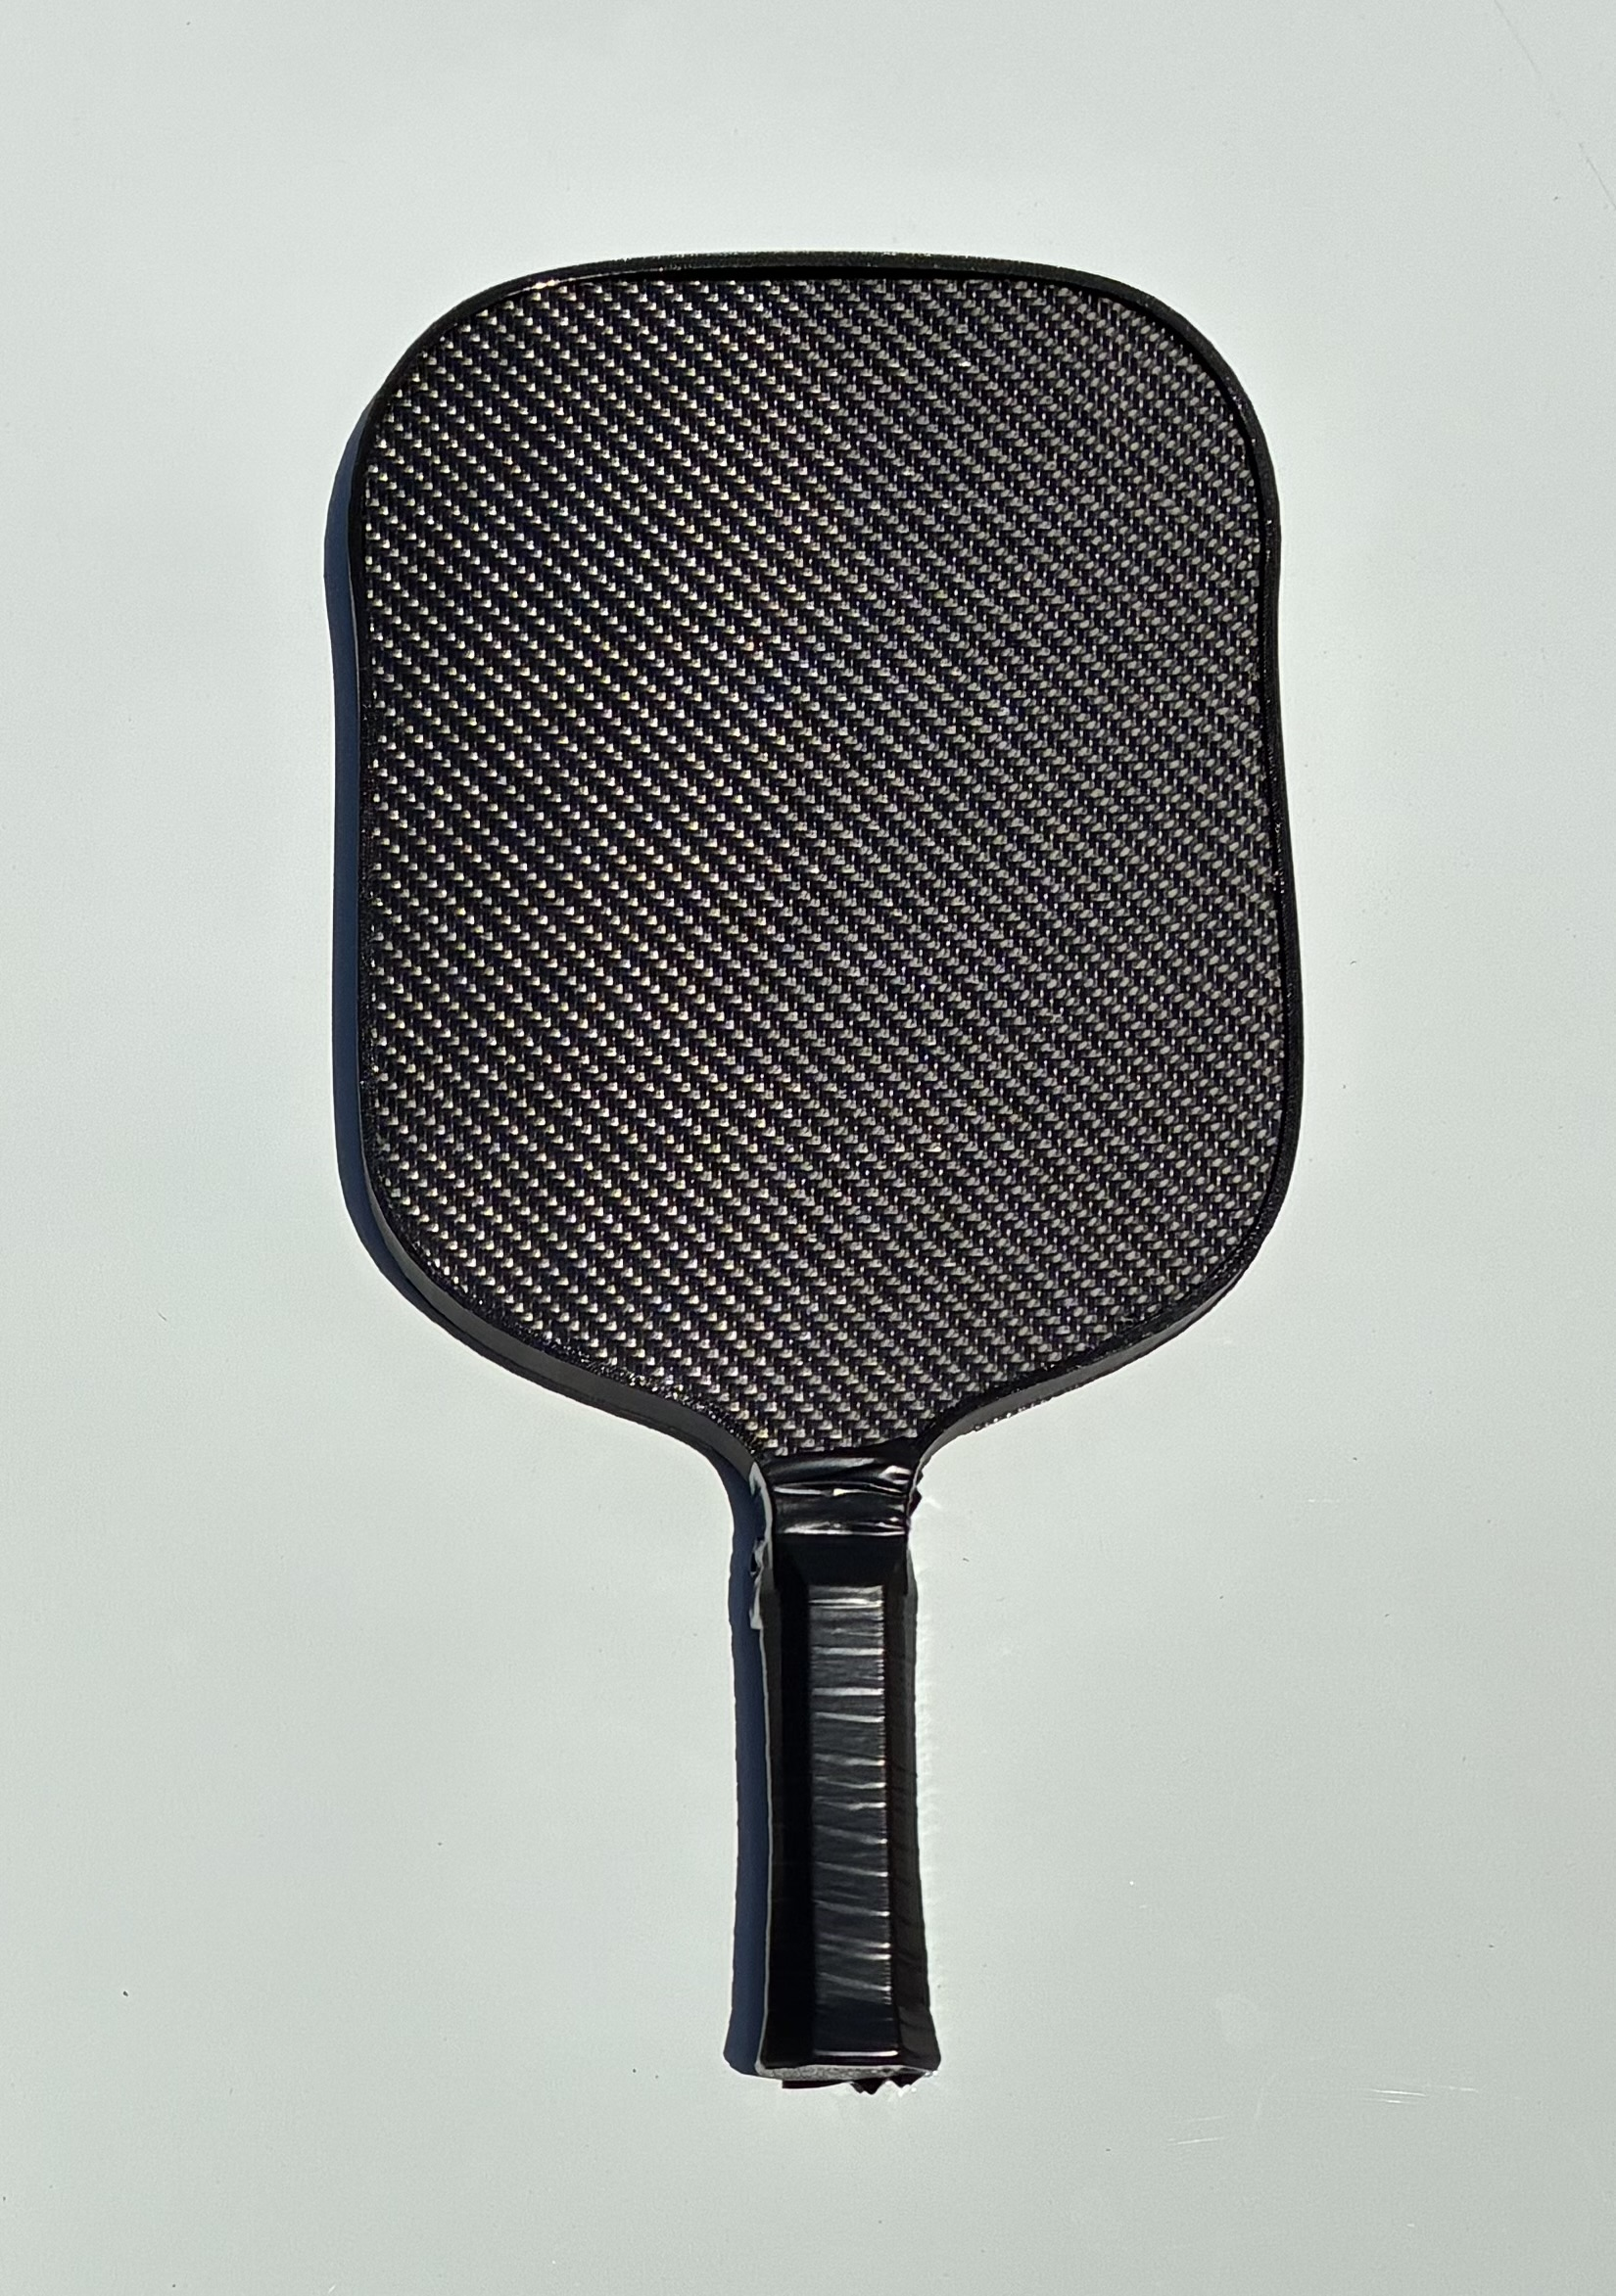
\includegraphics[
        width=3.72in,
        height=3.18in,
        keepaspectratio
    ]{full_assy}
};

\node[
    anchor=north,
    text=Muted,
    font=\sffamily\fontsize{6.9}{7.5}\selectfont
]
at ($(current page.north west)+(1.60in,-4.86in)$)
{Completed solo-built paddle assembly};

% ============================================================
% TOP CENTER — PROJECT OVERVIEW
% ============================================================

\fill[SoftGold,rounded corners=5pt]
    ($(current page.north west)+(2.95in,-1.62in)$)
    rectangle
    ($(current page.north west)+(5.53in,-4.86in)$);

\fill[PolyGold]
    ($(current page.north west)+(2.95in,-1.62in)$)
    rectangle
    ($(current page.north west)+(3.05in,-4.86in)$);

\node[
    anchor=north west,
    text=DeepGreen,
    font=\sffamily\bfseries\fontsize{8.0}{8.7}\selectfont
]
at ($(current page.north west)+(3.23in,-1.79in)$)
{PROJECT OVERVIEW};

\node[
    anchor=north west,
    align=left,
    text width=2.02in,
    text=Ink,
    font=\fontsize{7.05}{8.35}\selectfont
]
at ($(current page.north west)+(3.23in,-2.07in)$)
{
Independently designed and manufactured a lightweight prepreg
carbon-fiber pickleball paddle using a half-inch honeycomb
sandwich core, vacuum-bag consolidation, precision waterjet
trimming, and custom TPU and PLA components.

\vspace{5pt}

The project emphasized lightweight sandwich-composite design, repeatable manufacturing methods, dimensional accuracy, and the integration of custom 3D-printed TPU and PLA components into the final assembly.
};

\node[
    anchor=south west,
    align=left,
    text width=2.02in,
    text=PolyGold,
    font=\sffamily\bfseries\fontsize{6.65}{7.35}\selectfont
]
at ($(current page.north west)+(3.23in,-4.74in)$)
{
SOLE DESIGNER\\[2pt]
COMPOSITE FABRICATOR\\[2pt]
MANUFACTURING ENGINEER
};

% ============================================================
% TOP RIGHT — LAMINATE GRAPHIC
% ============================================================

\node[
    anchor=north west,
    inner sep=2.5pt,
    draw=DeepGreen,
    line width=0.65pt,
    rounded corners=5pt
]
at ($(current page.north west)+(5.71in,-1.62in)$)
{
    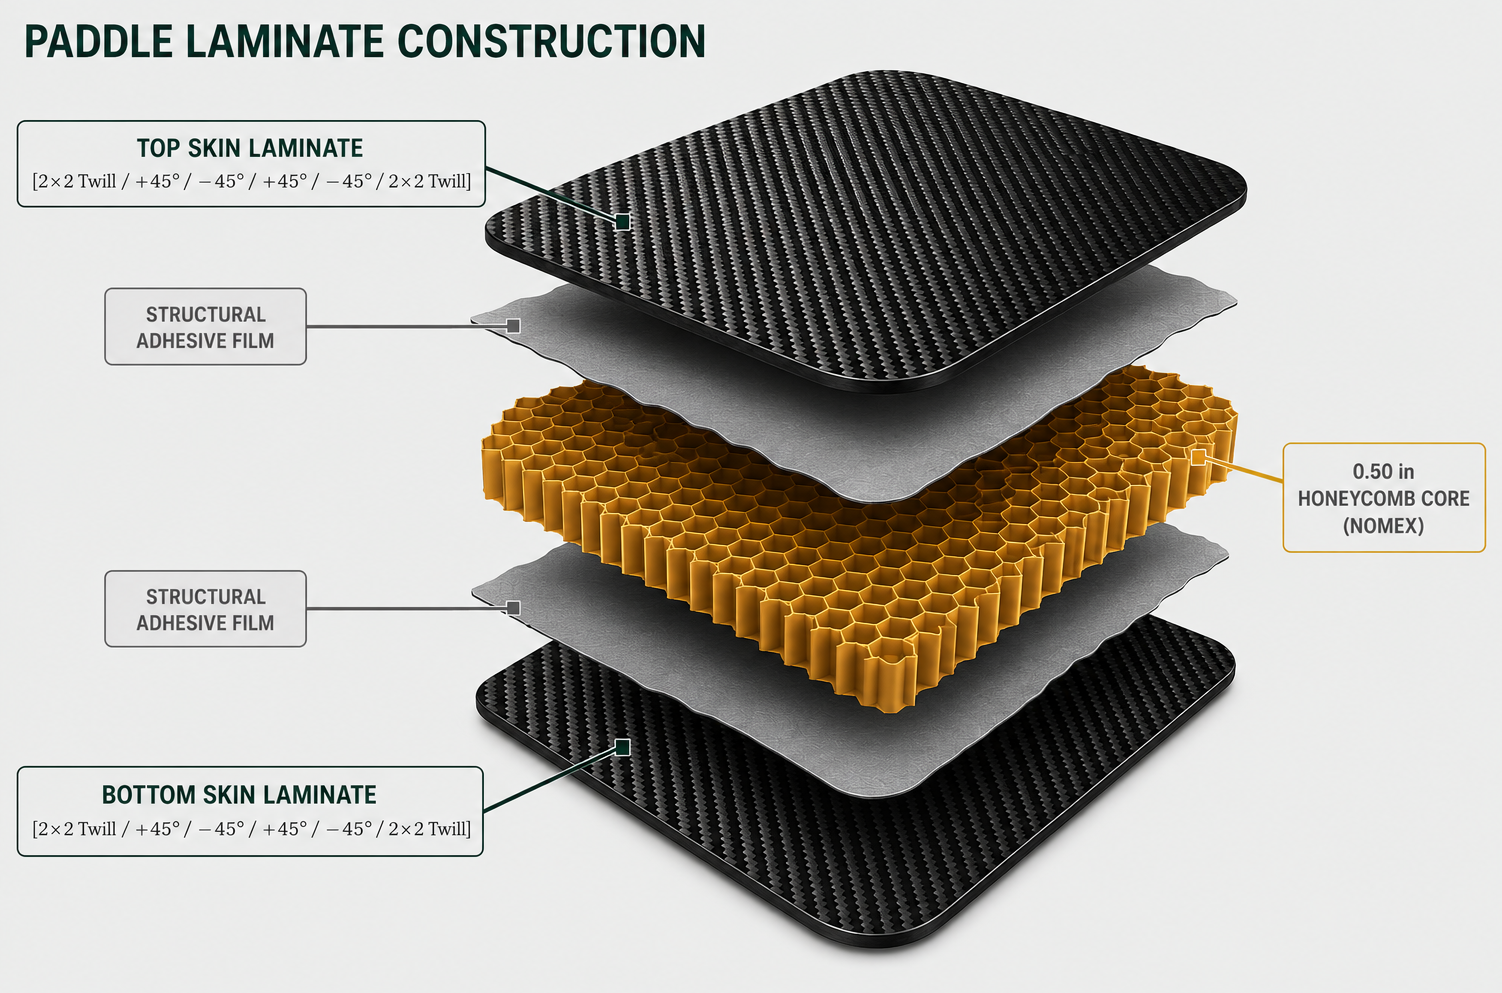
\includegraphics[
        width=4.80in,
        keepaspectratio
    ]{LAMINATE}
};

% ============================================================
% BOTTOM LEFT — SUPPORTING IMAGES
% ============================================================

\node[
    anchor=center,
    inner sep=3pt,
    draw=RuleGray,
    line width=0.55pt,
    rounded corners=4pt
]
at ($(current page.north west)+(1.12in,-5.98in)$)
{
    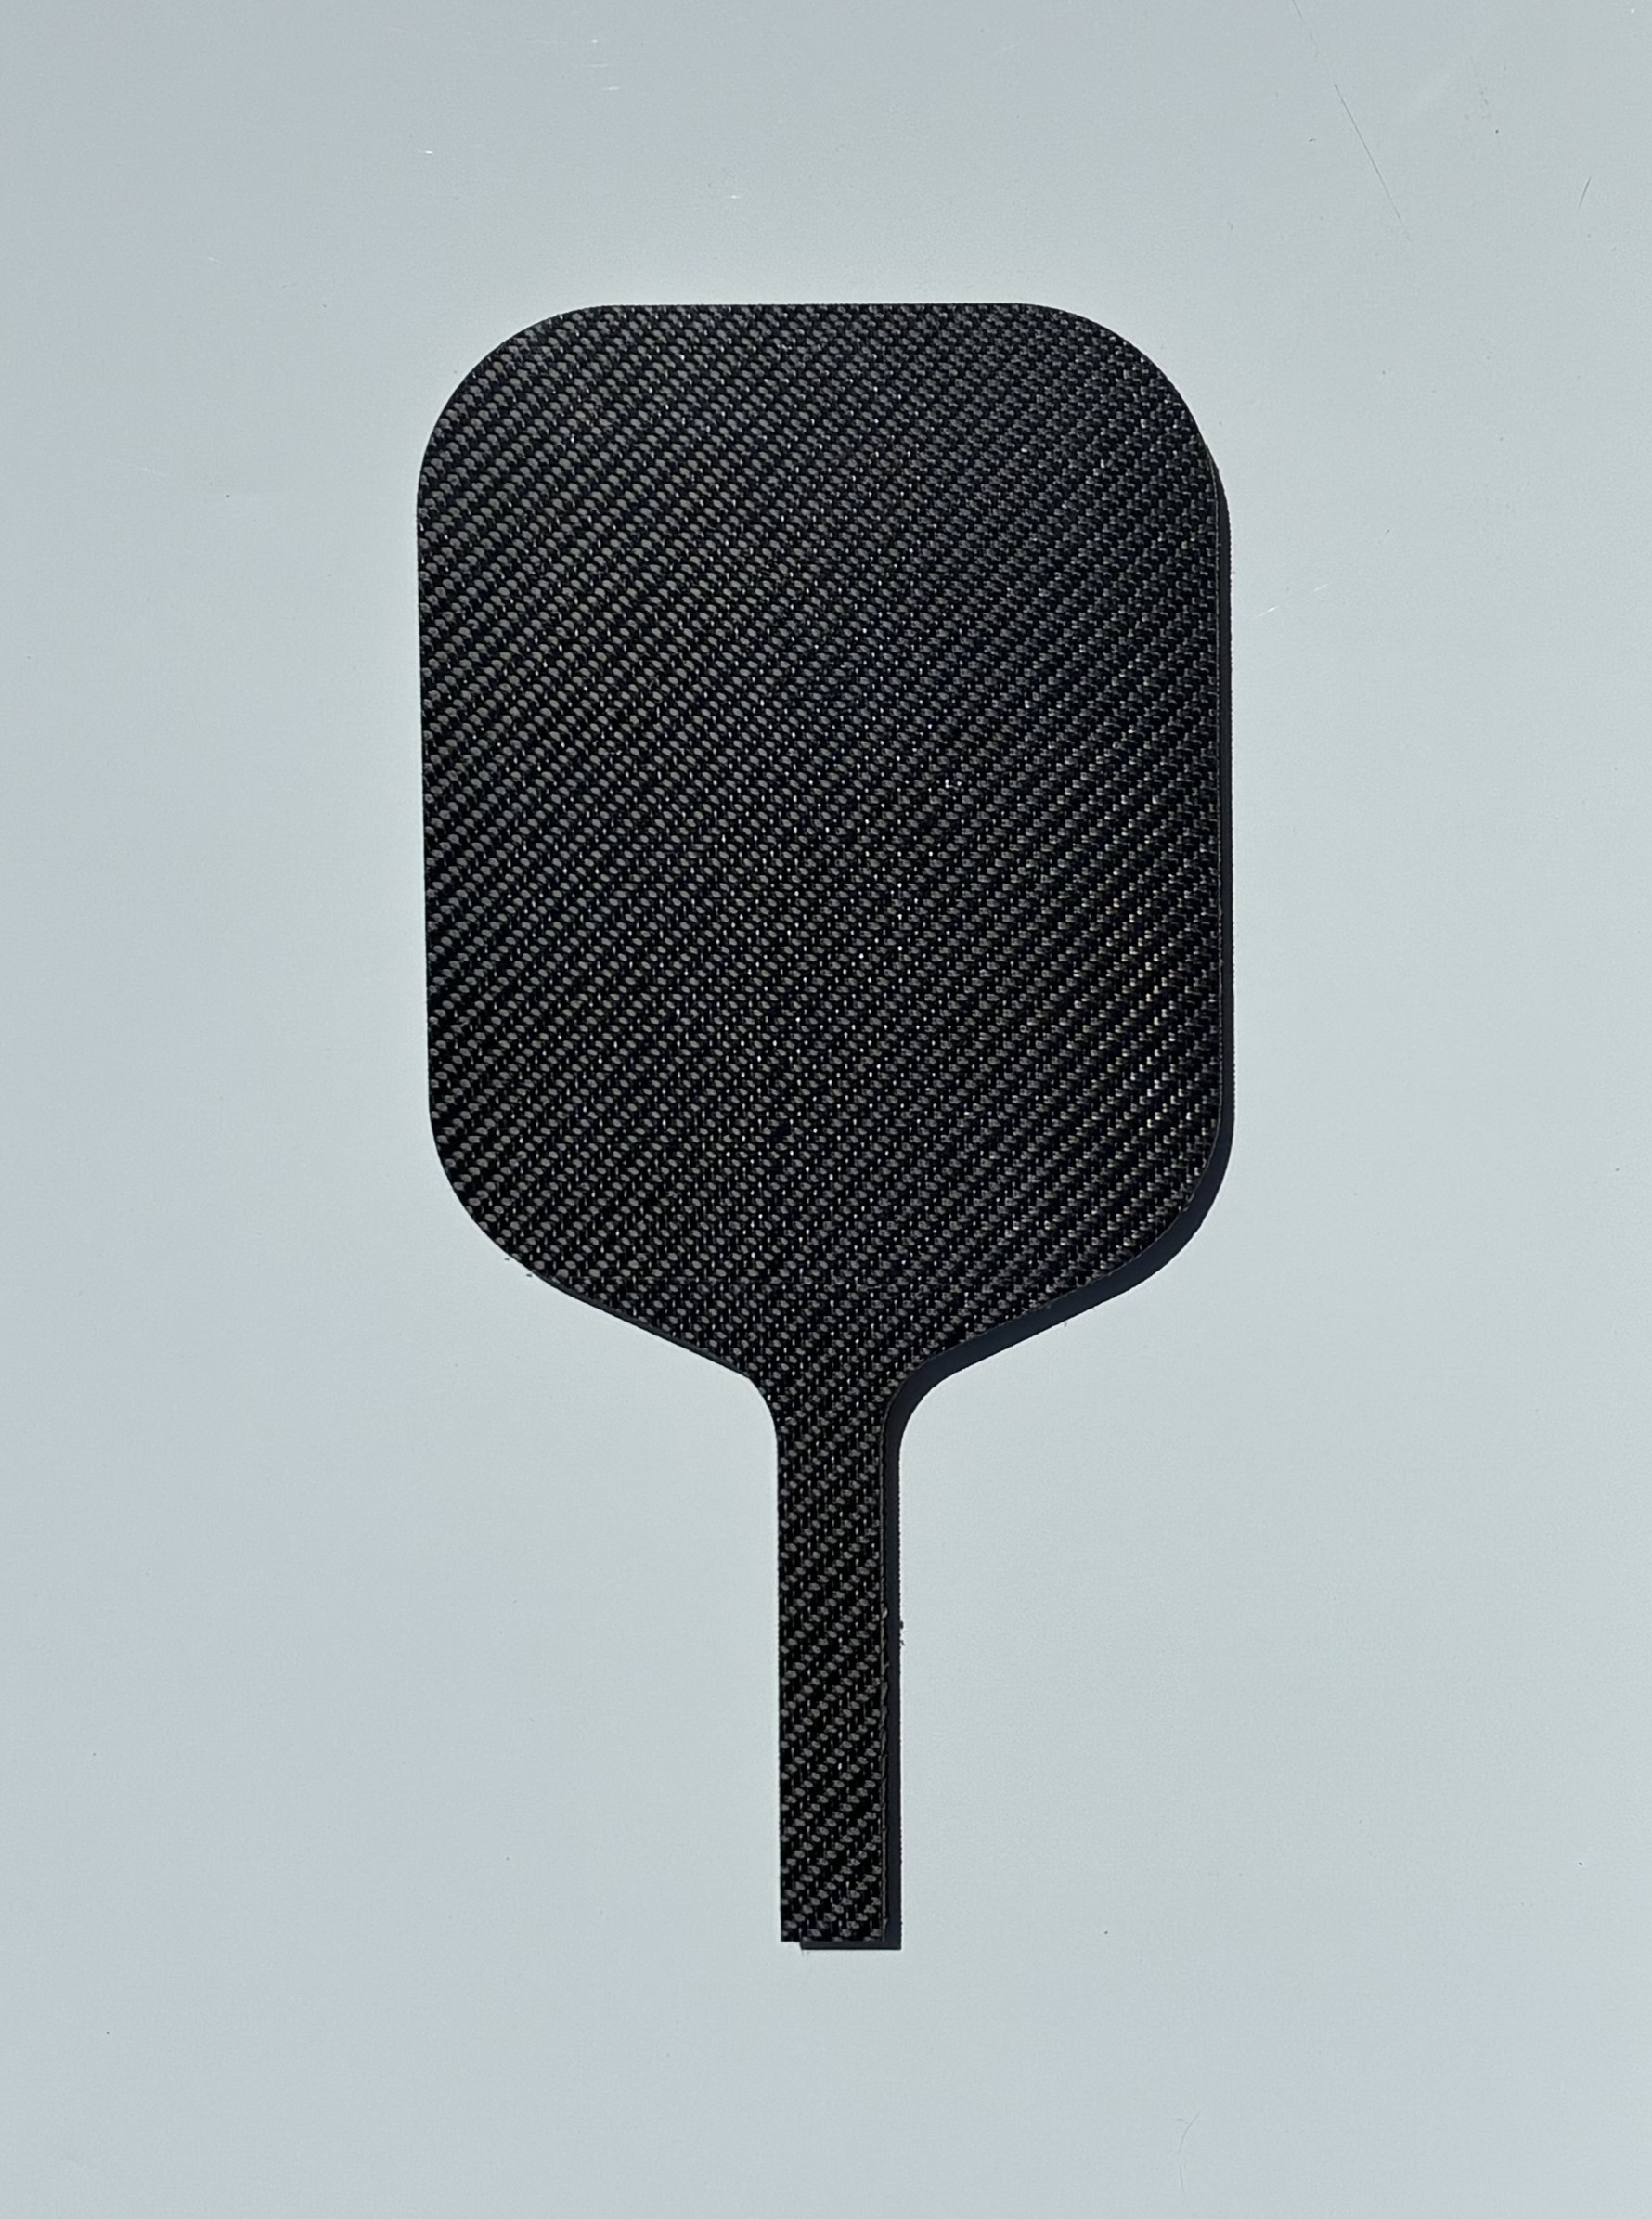
\includegraphics[
        width=1.30in,
        height=1.78in,
        keepaspectratio
    ]{front_view}
};

\node[
    anchor=center,
    inner sep=3pt,
    draw=RuleGray,
    line width=0.55pt,
    rounded corners=4pt
]
at ($(current page.north west)+(2.72in,-5.98in)$)
{
    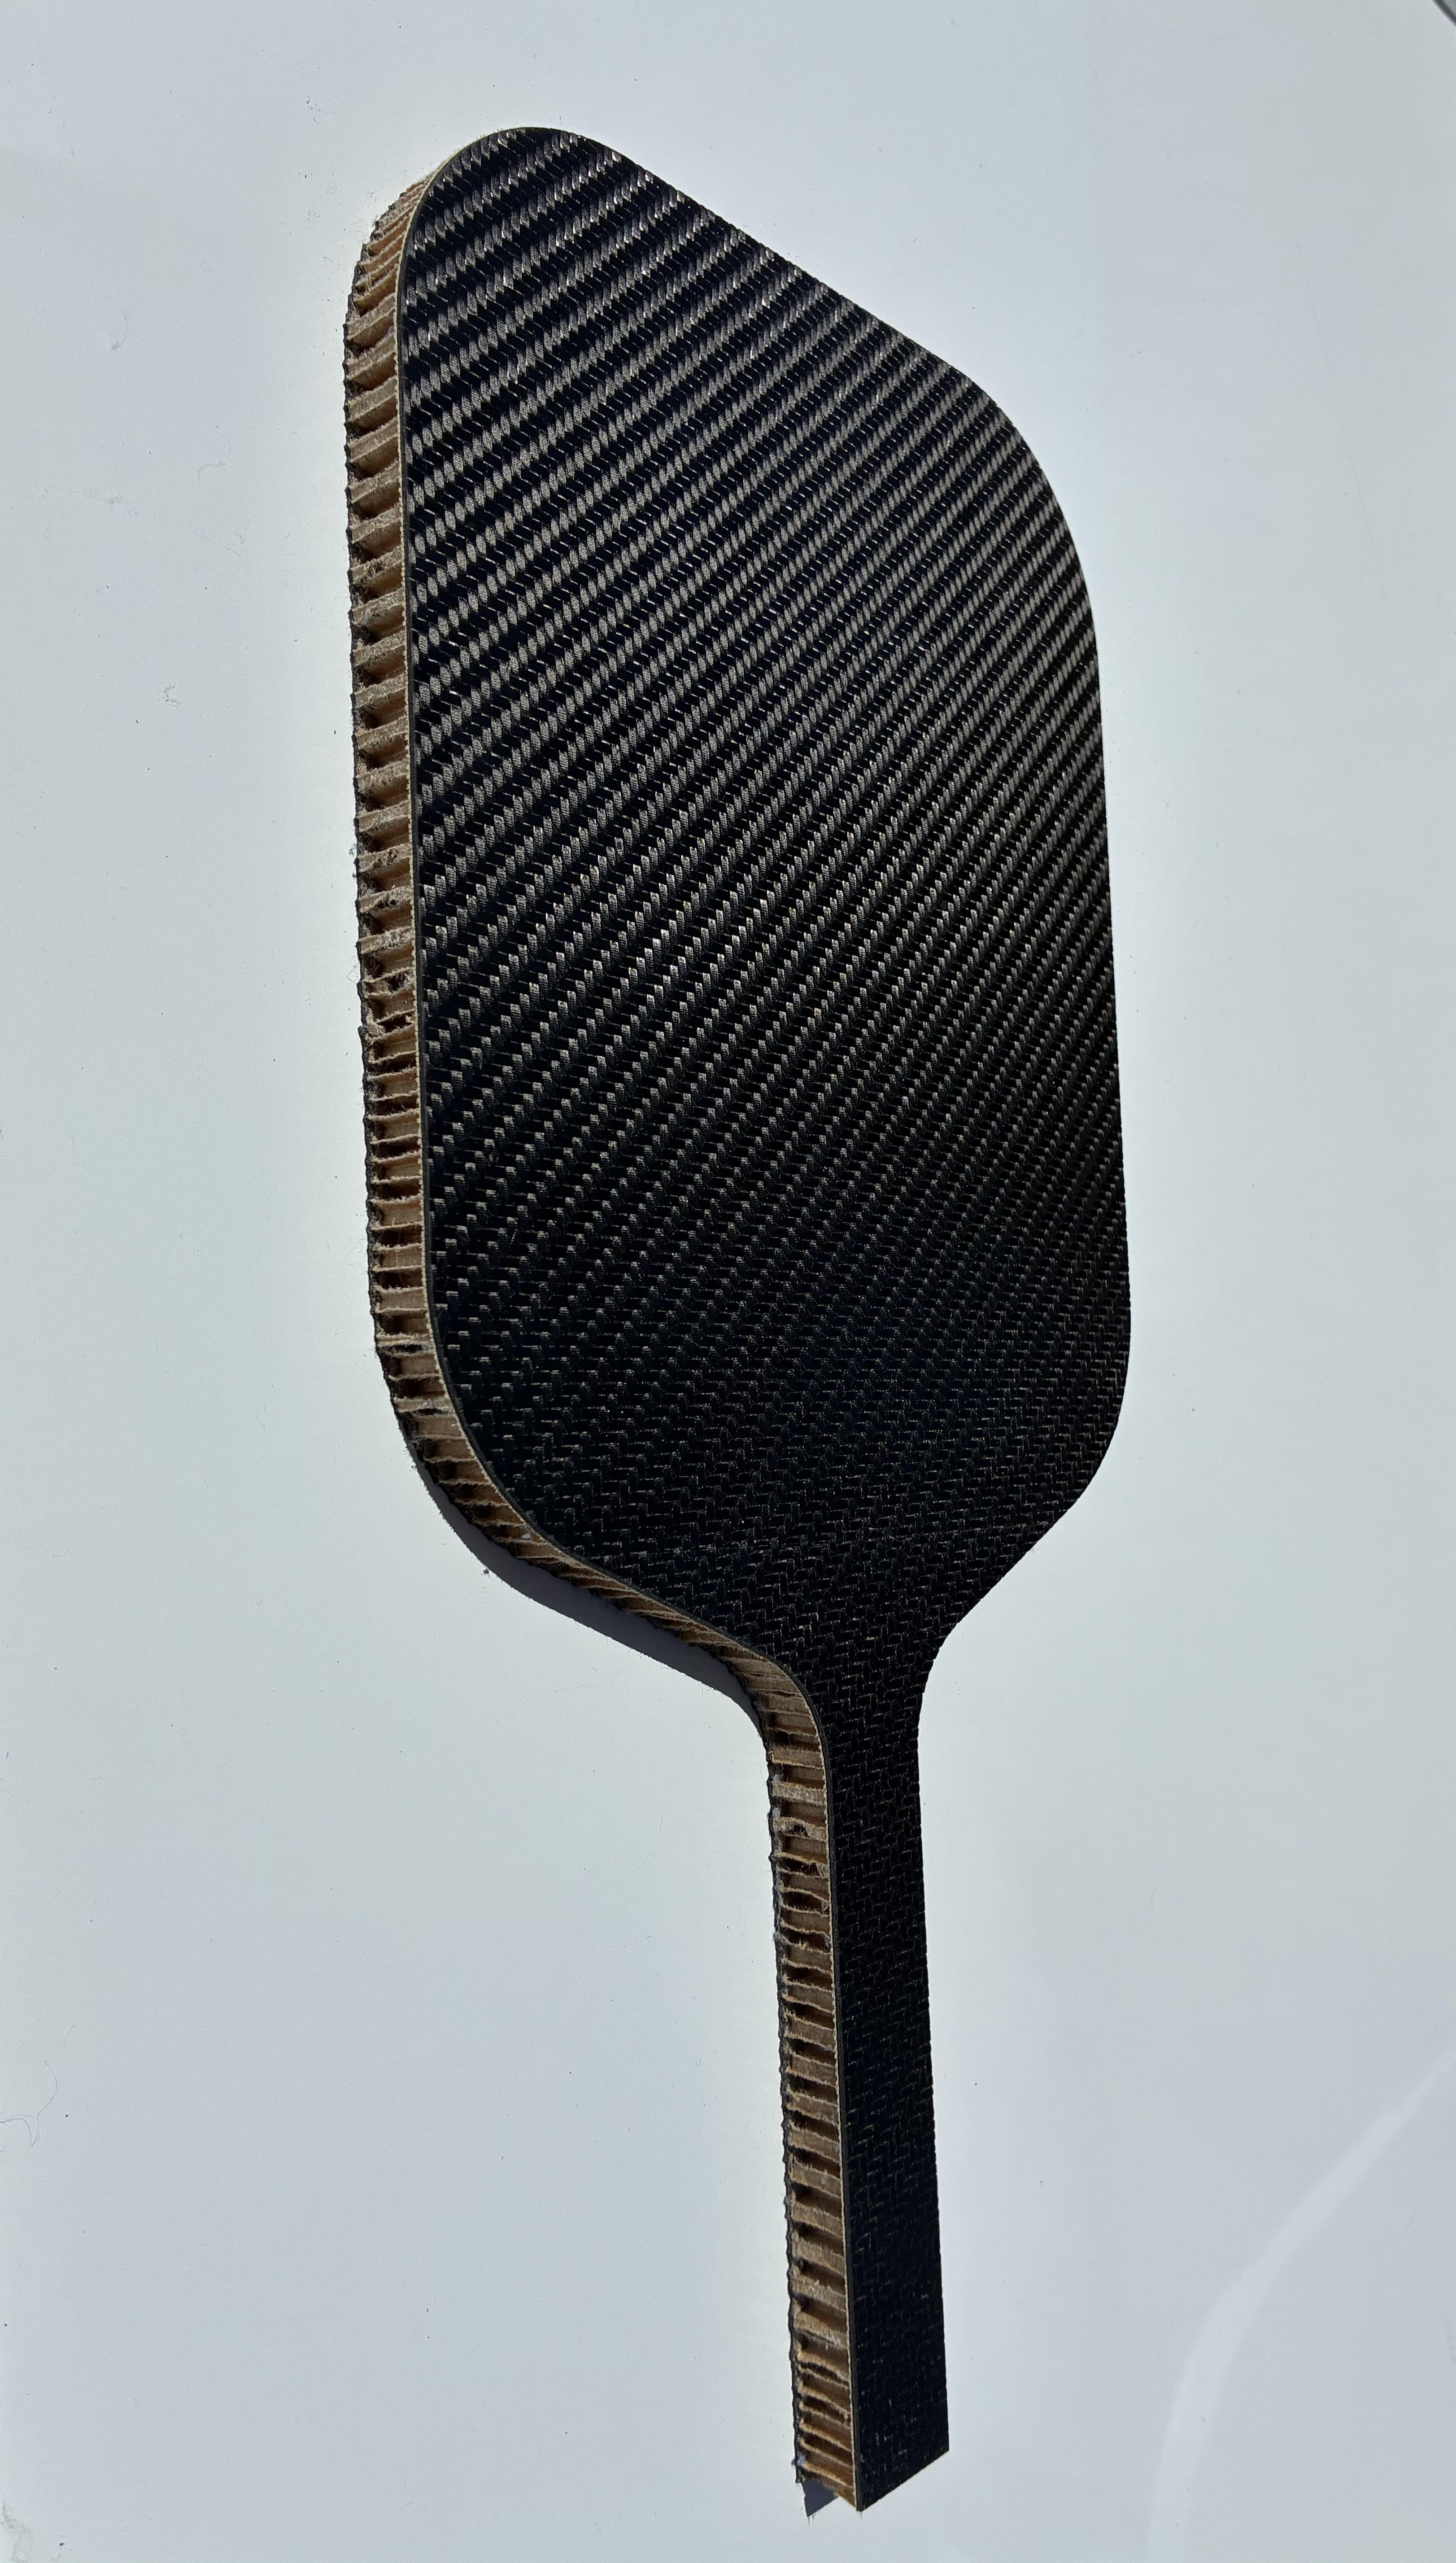
\includegraphics[
        width=1.30in,
        height=1.78in,
        keepaspectratio
    ]{side_core_view}
};

\node[
    anchor=center,
    inner sep=3pt,
    draw=RuleGray,
    line width=0.55pt,
    rounded corners=4pt
]
at ($(current page.north west)+(4.32in,-5.98in)$)
{
    \includegraphics[
        angle=-90,
        origin=c,
        width=1.30in,
        height=1.78in,
        keepaspectratio
    ]{waterjet}
};

\node[
    anchor=north,
    align=center,
    text width=1.38in,
    text=Muted,
    font=\sffamily\fontsize{6.5}{7.1}\selectfont
]
at ($(current page.north west)+(1.12in,-7.00in)$)
{Front view};

\node[
    anchor=north,
    align=center,
    text width=1.38in,
    text=Muted,
    font=\sffamily\fontsize{6.5}{7.1}\selectfont
]
at ($(current page.north west)+(2.72in,-7.00in)$)
{Core and edge profile};

\node[
    anchor=north,
    align=center,
    text width=1.38in,
    text=Muted,
    font=\sffamily\fontsize{6.5}{7.1}\selectfont
]
at ($(current page.north west)+(4.32in,-7.00in)$)
{Waterjet cutting setup};

% ============================================================
% BOTTOM RIGHT — MANUFACTURING HIGHLIGHTS
% ============================================================

\fill[SoftGreen,rounded corners=5pt]
    ($(current page.north west)+(5.18in,-5.05in)$)
    rectangle
    ($(current page.north east)+(-0.42in,-7.18in)$);

\draw[RuleGray,line width=0.55pt,rounded corners=5pt]
    ($(current page.north west)+(5.18in,-5.05in)$)
    rectangle
    ($(current page.north east)+(-0.42in,-7.18in)$);

\node[
    anchor=north west,
    text=DeepGreen,
    font=\sffamily\bfseries\fontsize{7.9}{8.6}\selectfont
]
at ($(current page.north west)+(5.44in,-5.20in)$)
{MANUFACTURING HIGHLIGHTS};

\node[
    anchor=north west,
    align=left,
    text width=5.05in,
    text=Ink,
    font=\fontsize{6.72}{7.82}\selectfont
]
at ($(current page.north west)+(5.44in,-5.49in)$)
{
\textbf{Consolidation.}
Vacuum bagging and distributed weight pressure maintained intimate contact
throughout the prepreg sandwich layup.\\[2.4pt]
\textbf{Surface quality.}
A scarce PTFE release film produced an unusually consistent matte finish
with a subtle sheen and minimal post-processing.\\[2.4pt]
\textbf{Waterjet stability.}
Perimeter weights restrained the cured stock against jet-induced lifting
and rotational moments during cutting.\\[2.4pt]
\textbf{Final assembly.}
A printed TPU edge band protected the carbon perimeter, while the PLA handle
used clearance cutouts to accommodate future stock-thickness and cutting variation.
};

% ============================================================
% RESOURCE LINK
% ============================================================

\node[
    anchor=north,
    align=center,
    text=DeepGreen,
    font=\sffamily\bfseries\fontsize{7.0}{7.6}\selectfont
]
at ($(current page.north)+(0,-7.42in)$)
{\href{\PaddleWaterjetVideo}
{\faPlayCircle\ WATERJET PICKLEBALL PADDLE DEMONSTRATION}};

% ============================================================
% FOOTER
% ============================================================

\node[
    anchor=south west,
    text=white,
    font=\sffamily\bfseries\fontsize{7.1}{7.7}\selectfont
]
at ($(current page.south west)+(0.42in,0.17in)$)
{\hyperlink{toro-results}{\faArrowLeft\ TORO COVER}};

\node[
    anchor=south,
    text=white,
    font=\sffamily\fontsize{7.0}{7.6}\selectfont
]
at ($(current page.south)+(0,0.17in)$)
{PICKLEBALL PADDLE \hspace{6pt} 1 / 1};

\node[
    anchor=south east,
    text=white,
    font=\sffamily\bfseries\fontsize{7.1}{7.7}\selectfont
]
at ($(current page.south east)+(-0.42in,0.17in)$)
{NEXT PROJECT \faArrowRight};

\end{tikzpicture}
%% ============================================================
% CARBON FIBER I-BEAM — SINGLE-PAGE PORTFOLIO CASE STUDY
% 01 Composites / Project 03
%
% IMPORTANT:
% 1. This file must NOT contain \documentclass, \begin{document},
%    or \end{document}.
% 2. In main.tex, place \input{ibeam_one_page} before \end{document}.
% 3. This script assumes the main portfolio preamble already defines:
%       DeepGreen, PolyGold, SoftGold, SoftGreen,
%       RuleGray, Muted, Ink
%    and loads tikz, graphicx, hyperref, and fontawesome5.
% 4. Upload these image files to Overleaf with the same names:
%       front view assembly graphic.png
%       Distributed weight with bolts.jpg
%       Stress Analysis on Generic CAD model.png
%       Beam Fiulure Delamination and cracking.jpeg
%       Three Point Bend Test.JPG
% ============================================================

\providecommand{\IBeamCompetitionGuidelines}
{https://drive.google.com/file/d/16S6MPVWWzPNKjXWVGKEySAi9i1f1BZYn/view?usp=sharing}

\providecommand{\IBeamBendTestVideo}
{https://drive.google.com/file/d/1LK_-pyK_y-a_4gDTiasz4uLUi95nAfrO/view?usp=drive_link}

\clearpage
\thispagestyle{empty}
\hypertarget{ibeam}{}
\null

\begin{tikzpicture}[remember picture,overlay]

% ============================================================
% BACKGROUND AND PAGE BARS
% ============================================================

\fill[white]
    (current page.south west)
    rectangle
    (current page.north east);

\fill[DeepGreen]
    (current page.north west)
    rectangle
    ($(current page.north east)+(0,-0.095in)$);

\fill[PolyGold]
    ($(current page.north west)+(0,-0.095in)$)
    rectangle
    ($(current page.north east)+(0,-0.14in)$);

\fill[DeepGreen]
    (current page.south west)
    rectangle
    ($(current page.south east)+(0,0.36in)$);

\fill[PolyGold]
    ($(current page.south west)+(0,0.36in)$)
    rectangle
    ($(current page.south east)+(0,0.405in)$);

% ============================================================
% HEADER
% ============================================================

\node[
    anchor=north west,
    text=PolyGold,
    font=\sffamily\bfseries\fontsize{8.1}{8.7}\selectfont
]
at ($(current page.north west)+(0.42in,-0.39in)$)
{01 COMPOSITES \hspace{5pt}/\hspace{5pt} PROJECT 03};

\node[
    anchor=north west,
    text=DeepGreen,
    font=\bfseries\fontsize{22.3}{23.3}\selectfont
]
at ($(current page.north west)+(0.40in,-0.67in)$)
{CARBON FIBER I-BEAM DESIGN \& TESTING};

\node[
    anchor=north west,
    text=Muted,
    font=\sffamily\fontsize{8.25}{9.0}\selectfont
]
at ($(current page.north west)+(0.42in,-1.12in)$)
{Cal Poly Composites Laboratory \hspace{7pt}\textbullet\hspace{7pt}
Individual Project \hspace{7pt}\textbullet\hspace{7pt}
Winter 2026 \hspace{7pt}\textbullet\hspace{7pt}
San Luis Obispo, California};

\fill[PolyGold]
    ($(current page.north west)+(0.42in,-1.36in)$)
    rectangle
    ($(current page.north west)+(6.10in,-1.315in)$);


% ============================================================
% TOP LEFT — ASSEMBLY ARCHITECTURE
% ============================================================

\node[
    anchor=north west,
    inner sep=2.6pt,
    draw=DeepGreen,
    line width=0.68pt,
    rounded corners=5pt
]
at ($(current page.north west)+(0.42in,-1.58in)$)
{
    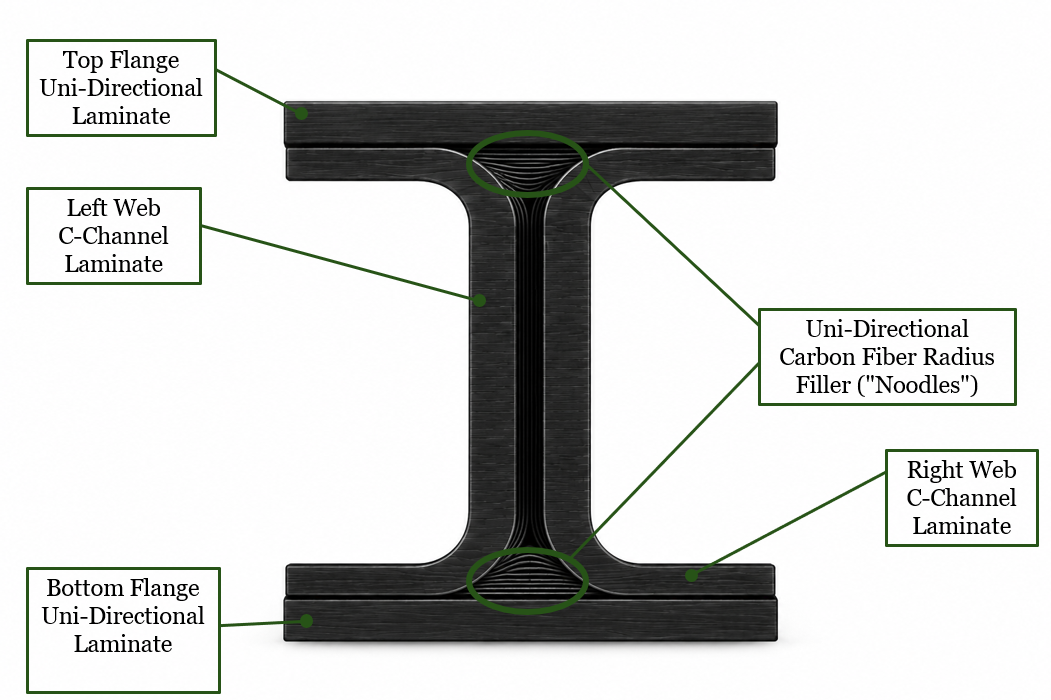
\includegraphics[
        width=3.55in,
        height=2.45in,
        keepaspectratio
    ]{front view assembly graphic.png}
};

\node[
    anchor=north,
    align=center,
    inner sep=0pt,
    text width=3.42in,
    text=Muted,
    font=\sffamily\fontsize{6.35}{7.05}\selectfont
]
at ($(current page.north west)+(2.195in,-4.12in)$)
{Four-piece laminate architecture with top and bottom flange laminates, paired C-channels, and longitudinal radius fillers};

% ============================================================
% TOP CENTER — PROJECT OVERVIEW + C-CHANNEL LAYUP
% ============================================================

\fill[SoftGold,rounded corners=5pt]
    ($(current page.north west)+(4.18in,-1.58in)$)
    rectangle
    ($(current page.north west)+(7.42in,-4.20in)$);

\fill[PolyGold]
    ($(current page.north west)+(4.18in,-1.58in)$)
    rectangle
    ($(current page.north west)+(4.28in,-4.20in)$);

\node[
    anchor=north west,
    text=DeepGreen,
    font=\sffamily\bfseries\fontsize{8.0}{8.7}\selectfont
]
at ($(current page.north west)+(4.48in,-1.76in)$)
{PROJECT OVERVIEW};

\node[
    anchor=north west,
    align=left,
    text width=2.64in,
    text=Ink,
    font=\fontsize{6.40}{7.45}\selectfont
]
at ($(current page.north west)+(4.48in,-2.04in)$)
{
A 24-inch carbon-fiber I-beam was manufactured from two molded
C-channel laminates, separate top and bottom flange laminates,
and longitudinal unidirectional radius fillers. The completed
684 g specimen sustained 28.2 kN (6,340 lbf) in three-point bending.\\[3pt]
\textbf{C-channel layup.}
Each channel used the same 12-ply sequence:
\mbox{$[+45/-45/0/+45/-45/0/0/-45/+45/0/-45/+45]$}.
The layup was completed twice, once for each channel.\\[3pt]
\textbf{Flange layups.}
Top flange: \mbox{$[90/0_6/90/0_6]$}. Bottom flange:
\mbox{$[90/0_6]$}, where $0_6$ denotes six consecutive 0-degree plies.
};

\node[
    anchor=south west,
    text=PolyGold,
    font=\sffamily\bfseries\fontsize{6.45}{7.1}\selectfont
]
at ($(current page.north west)+(4.48in,-4.03in)$)
{MASS: 684 g \hspace{8pt}\textbullet\hspace{8pt} PEAK LOAD: 28.2 kN \hspace{8pt}\textbullet\hspace{8pt} LENGTH: 24 in};

% ============================================================
% TOP RIGHT — C-CHANNEL MANUFACTURING
% ============================================================

\node[
    anchor=north west,
    inner sep=2.6pt,
    draw=DeepGreen,
    line width=0.68pt,
    rounded corners=5pt
]
at ($(current page.north west)+(7.62in,-1.58in)$)
{
    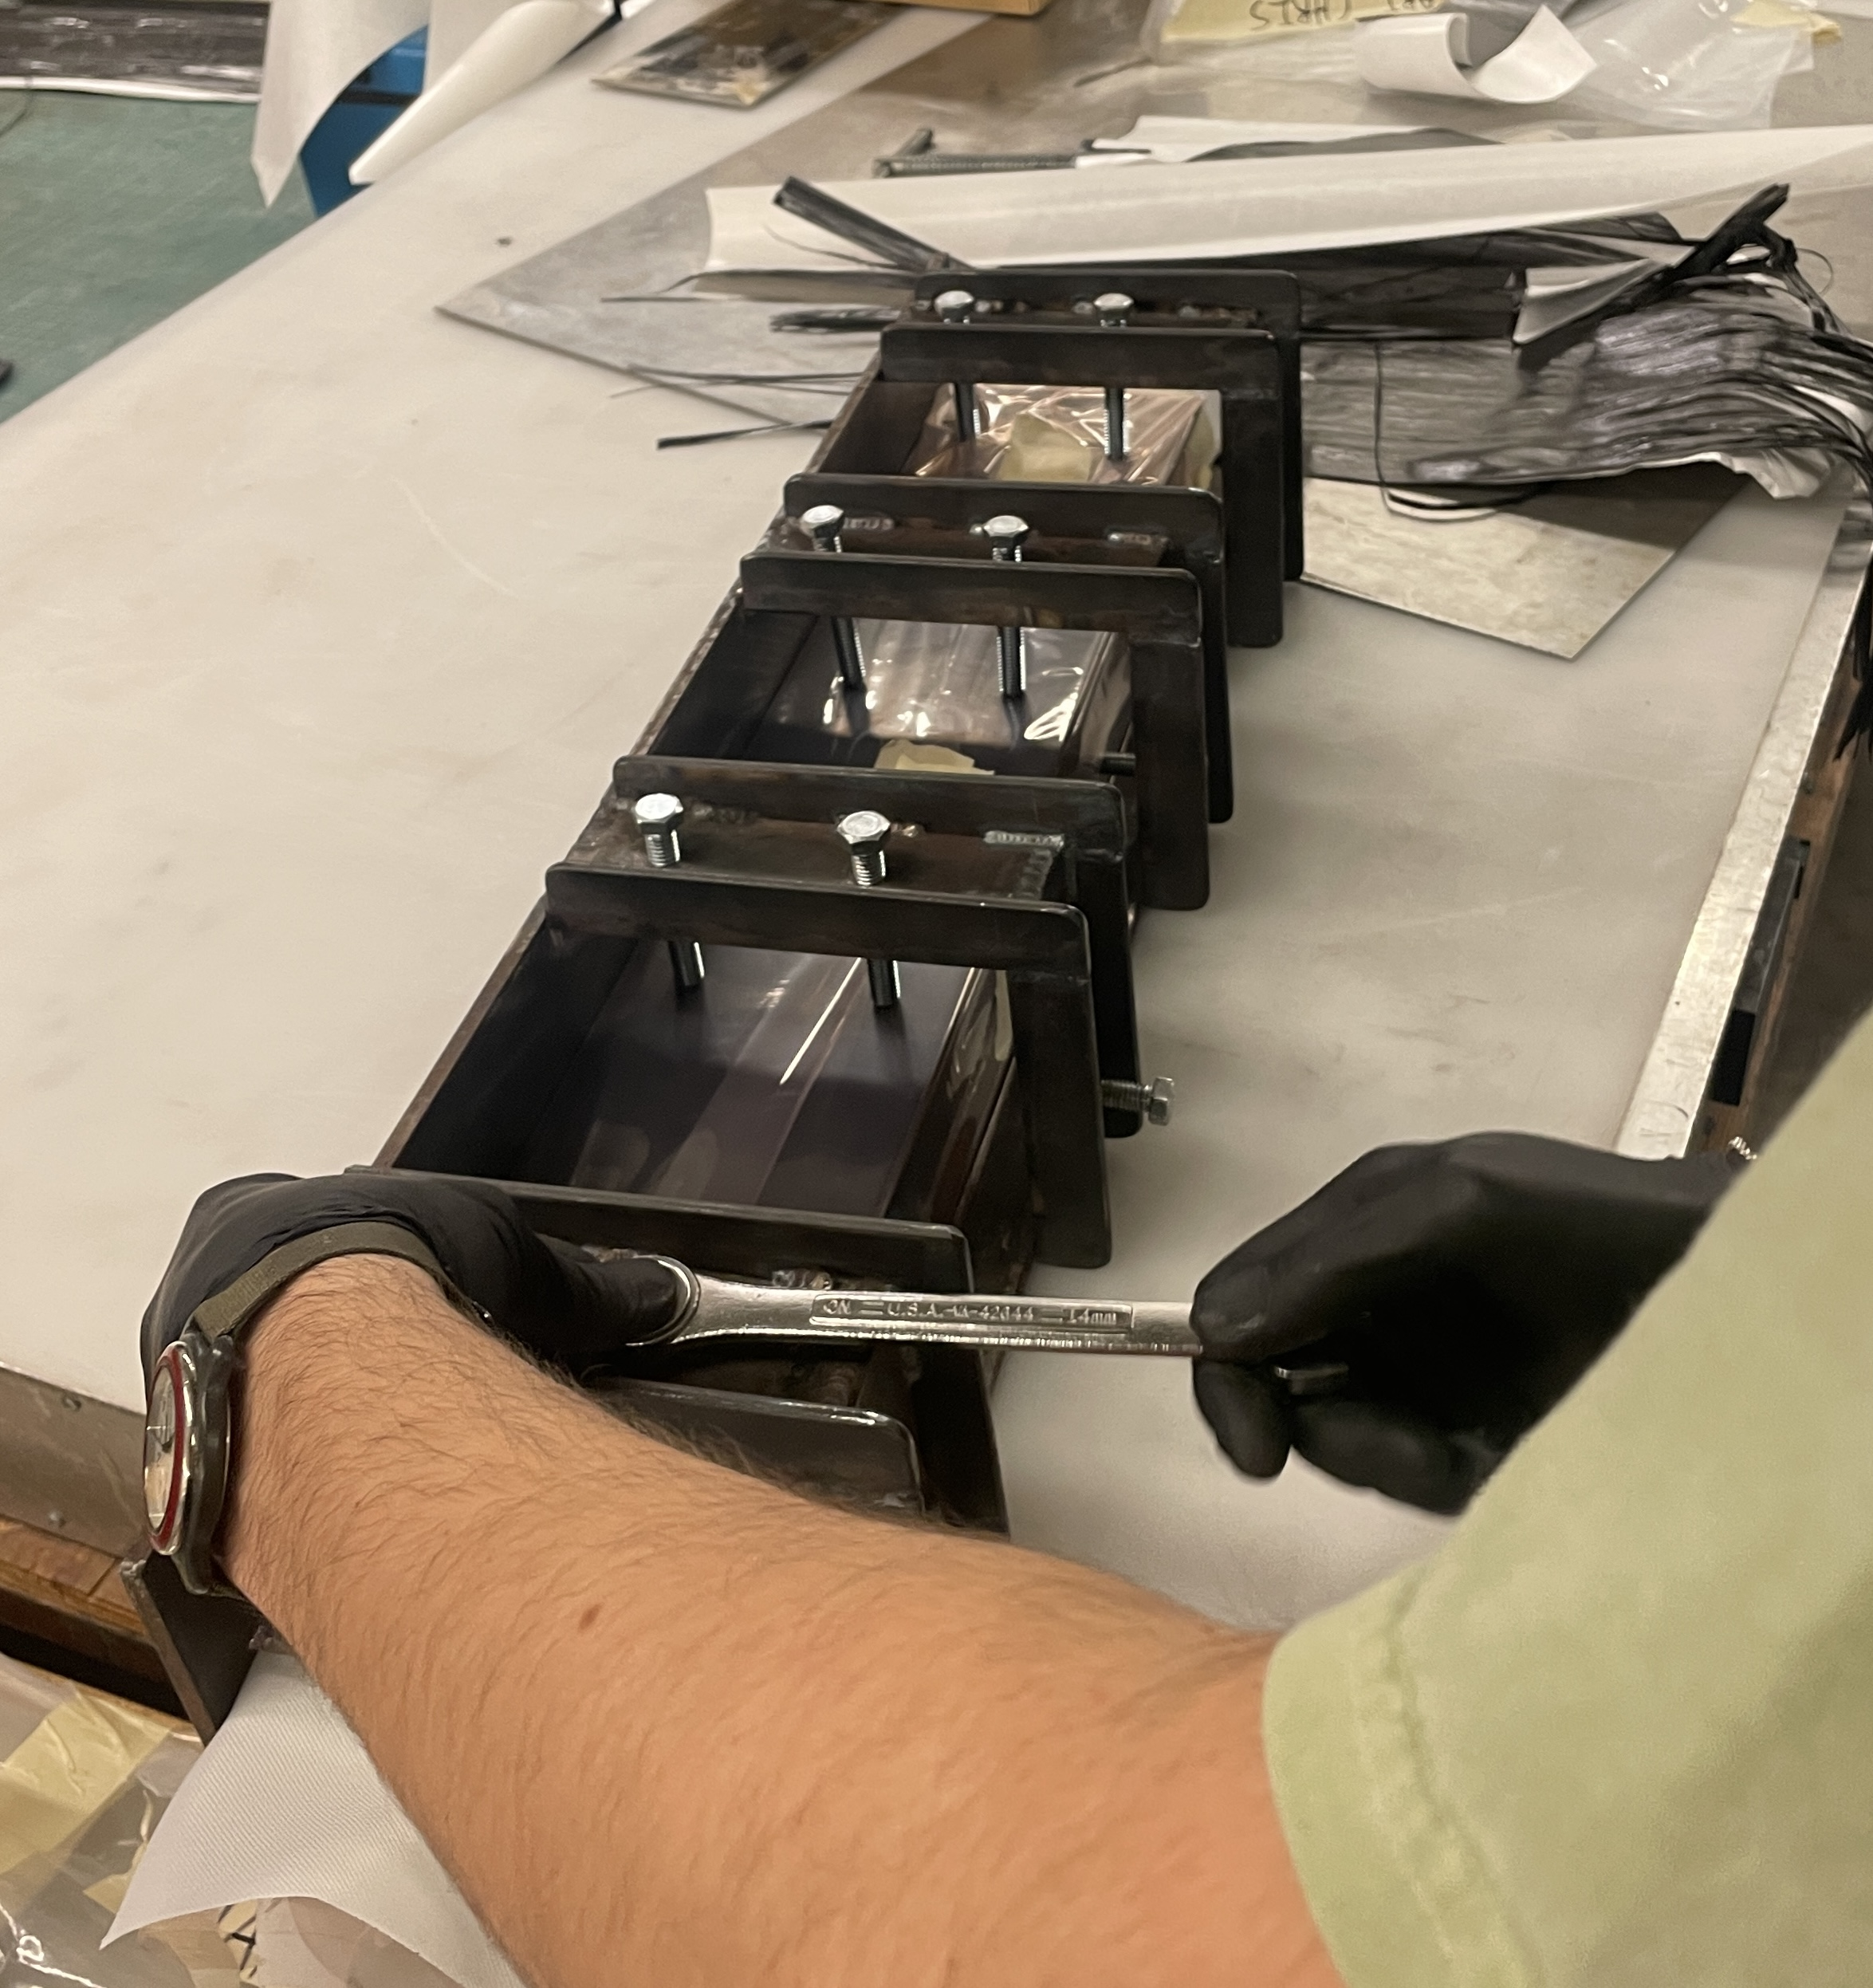
\includegraphics[
        width=3.55in,
        height=2.45in,
        keepaspectratio
    ]{Distributed weight with bolts.jpg}
};

\node[
    anchor=north,
    align=center,
    inner sep=0pt,
    text width=3.42in,
    text=Muted,
    font=\sffamily\fontsize{6.35}{7.05}\selectfont
]
at ($(current page.north west)+(9.395in,-4.12in)$)
{Distributed bolt pressure maintained alignment and consolidated the full beam assembly during cure};

% ============================================================
% CENTER ROW — MODEL, TEST, AND OBSERVED FAILURE
% ============================================================

\node[
    anchor=north west,
    inner sep=2.4pt,
    draw=RuleGray,
    line width=0.55pt,
    rounded corners=4pt
]
at ($(current page.north west)+(0.42in,-4.43in)$)
{
    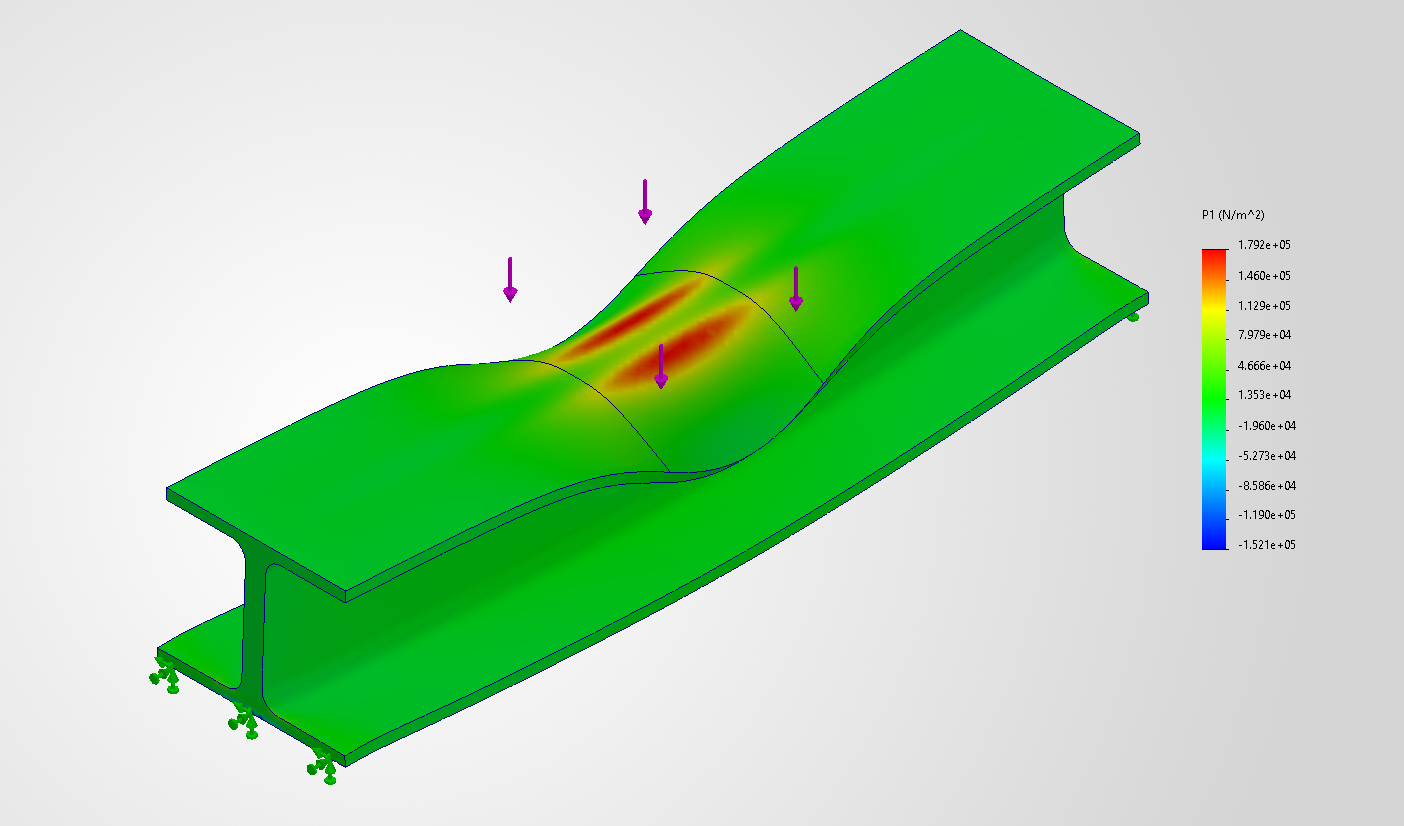
\includegraphics[
        width=3.33in,
        height=1.62in,
        keepaspectratio
    ]{Stress Analysis on Generic CAD model.png}
};

\node[
    anchor=north,
    align=center,
    inner sep=0pt,
    text width=3.20in,
    text=Muted,
    font=\sffamily\fontsize{6.20}{6.85}\selectfont
]
at ($(current page.north west)+(2.085in,-6.14in)$)
{Generic FEA predicted peak compressive stress beneath the center loading shoe};

\node[
    anchor=north west,
    inner sep=2.4pt,
    draw=RuleGray,
    line width=0.55pt,
    rounded corners=4pt
]
at ($(current page.north west)+(3.92in,-4.43in)$)
{
    \includegraphics[
        angle=180,
        origin=c,
        width=3.18in,
        height=1.62in,
        keepaspectratio
    ]{Three Point Bend Test.JPG}
};

\node[
    anchor=north,
    align=center,
    inner sep=0pt,
    text width=3.05in,
    text=Muted,
    font=\sffamily\fontsize{6.20}{6.85}\selectfont
]
at ($(current page.north west)+(5.510in,-6.14in)$)
{Experimental three-point bend test on the completed I-beam specimen};

\node[
    anchor=north west,
    inner sep=2.4pt,
    draw=RuleGray,
    line width=0.55pt,
    rounded corners=4pt
]
at ($(current page.north west)+(7.28in,-4.43in)$)
{
    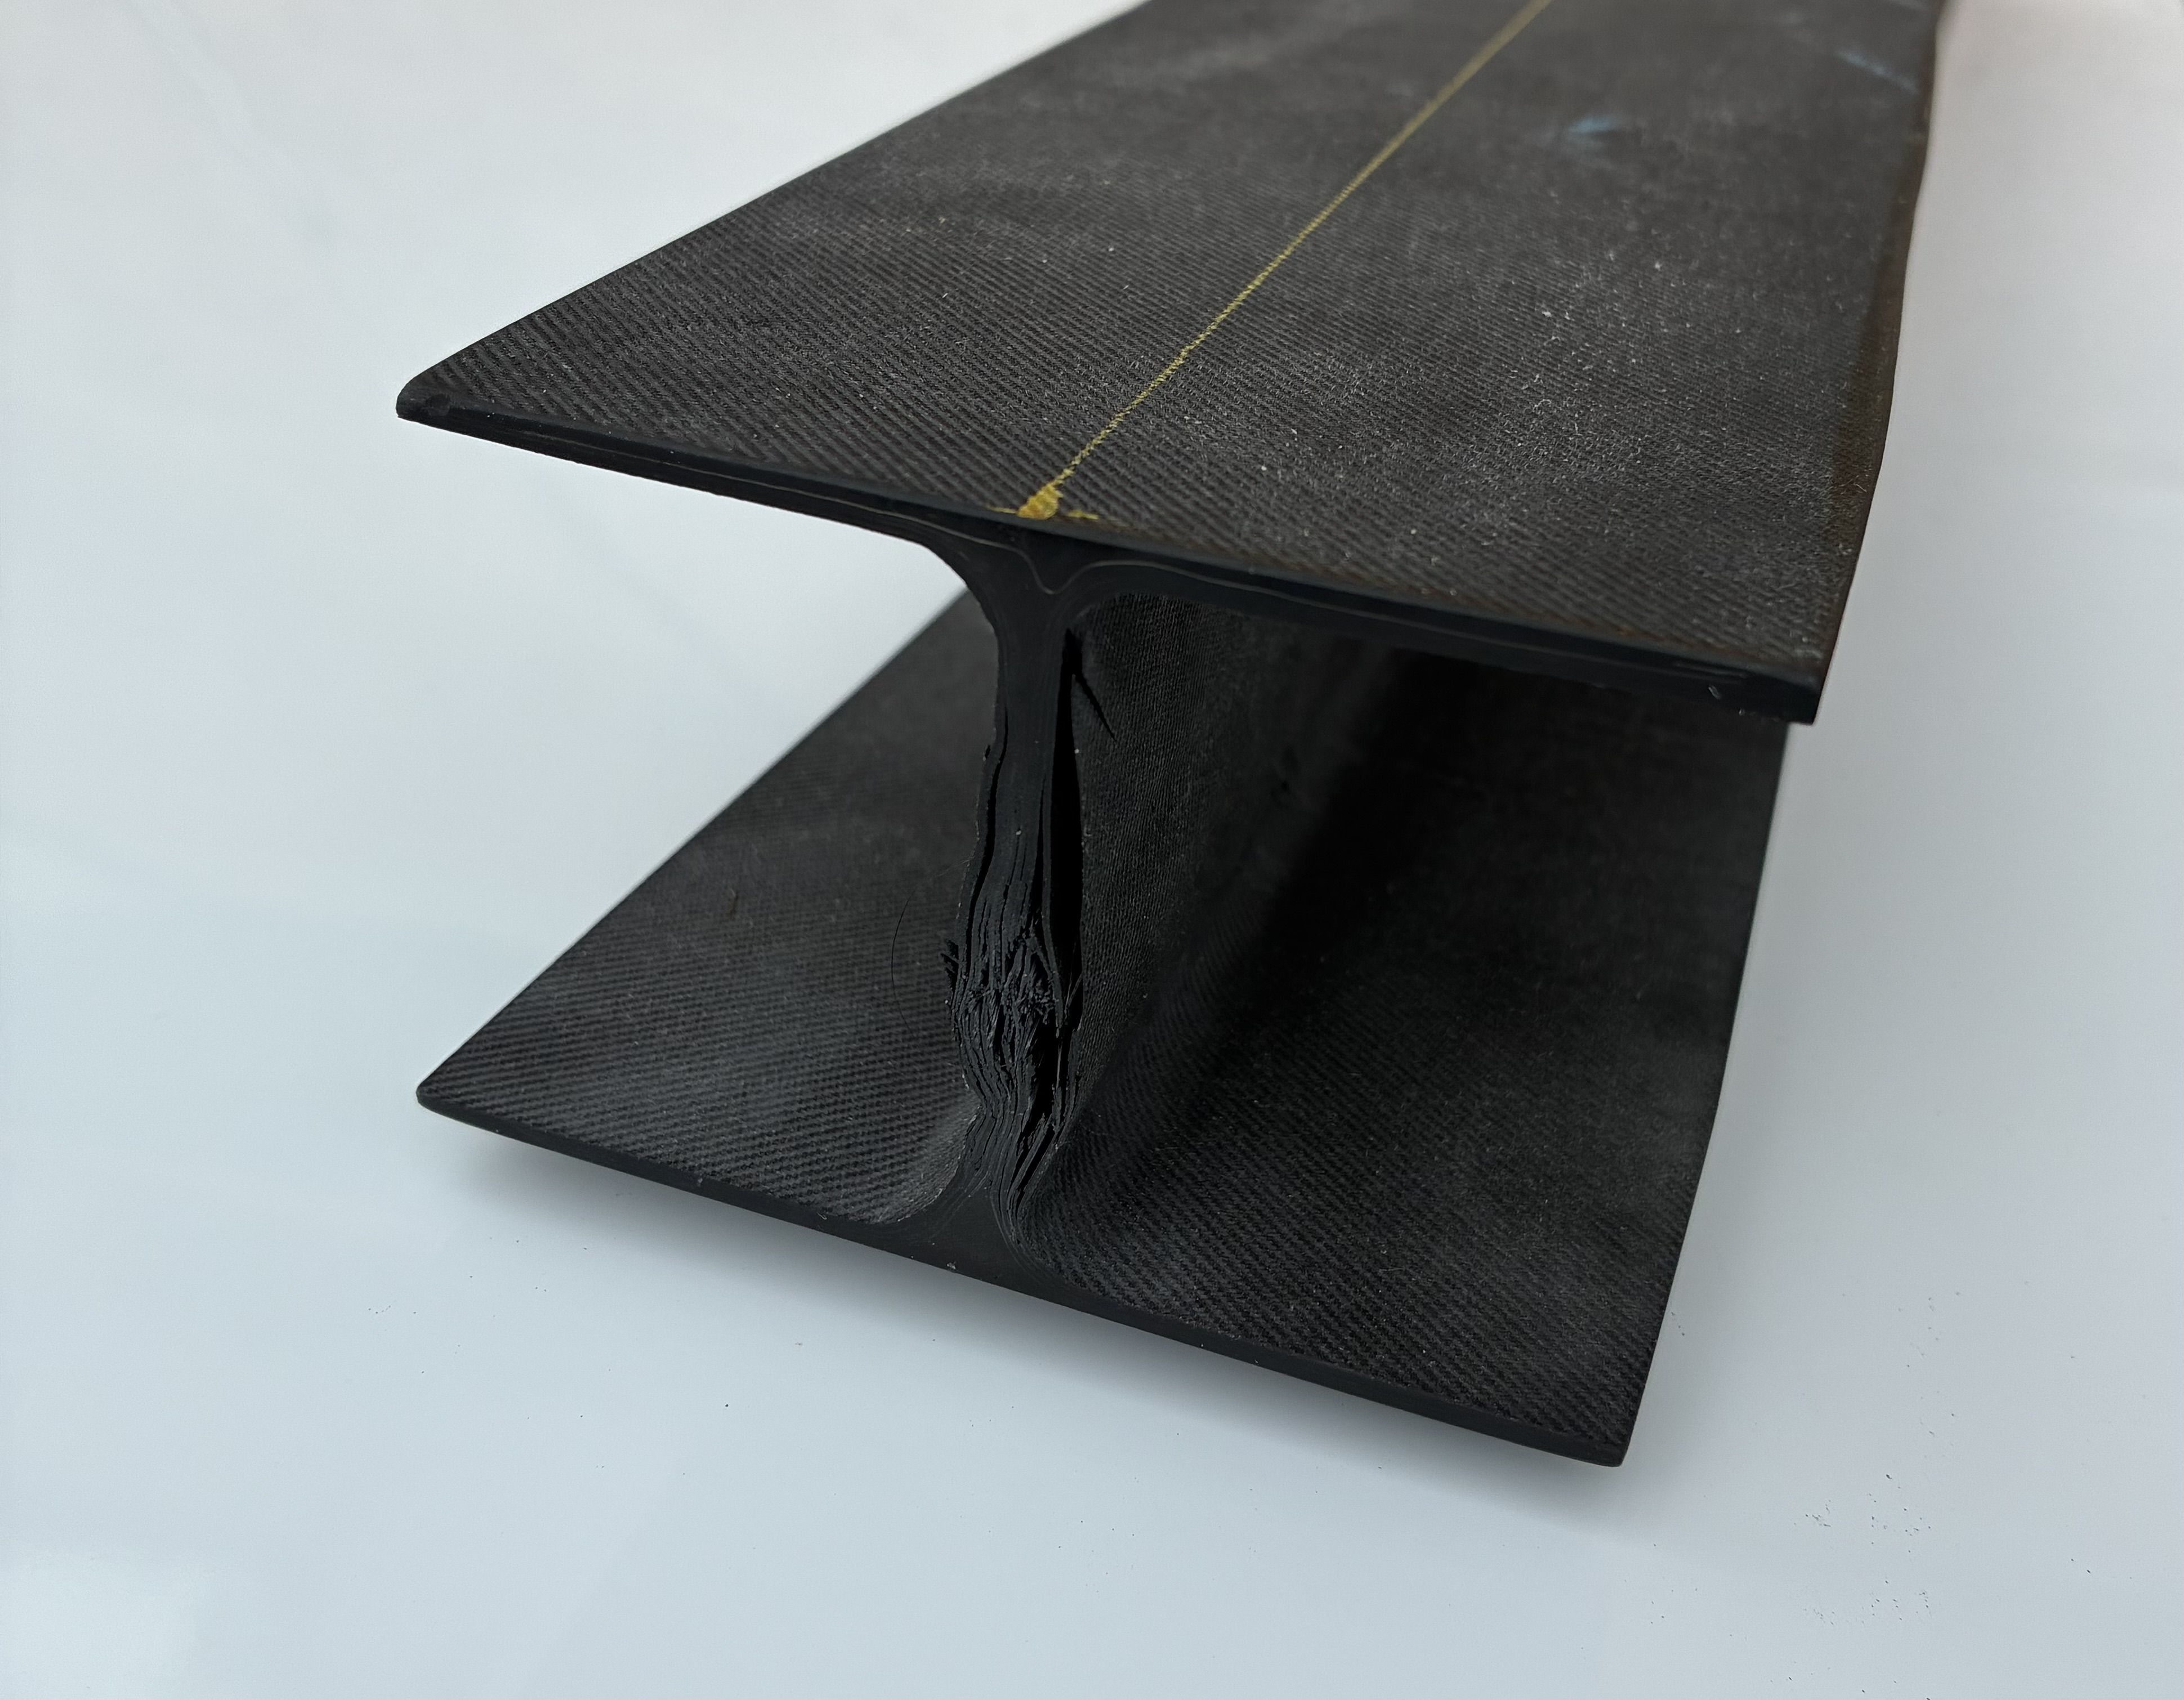
\includegraphics[
        width=3.65in,
        height=1.62in,
        keepaspectratio
    ]{Beam Fiulure Delamination and cracking.jpeg}
};

\node[
    anchor=north,
    align=center,
    inner sep=0pt,
    text width=3.50in,
    text=Muted,
    font=\sffamily\fontsize{6.20}{6.85}\selectfont
]
at ($(current page.north west)+(9.105in,-6.14in)$)
{Observed edge failure with delamination and longitudinal crack propagation};

% ============================================================
% BOTTOM LEFT — MANUFACTURING PROCESS
% ============================================================

\fill[SoftGreen,rounded corners=5pt]
    ($(current page.north west)+(0.42in,-6.43in)$)
    rectangle
    ($(current page.north west)+(5.30in,-7.18in)$);

\draw[RuleGray,line width=0.55pt,rounded corners=5pt]
    ($(current page.north west)+(0.42in,-6.43in)$)
    rectangle
    ($(current page.north west)+(5.30in,-7.18in)$);

\node[
    anchor=north west,
    text=DeepGreen,
    font=\sffamily\bfseries\fontsize{7.65}{8.35}\selectfont
]
at ($(current page.north west)+(0.66in,-6.57in)$)
{MANUFACTURING APPROACH};

\node[
    anchor=north west,
    align=left,
    text width=4.38in,
    text=Ink,
    font=\fontsize{6.20}{7.15}\selectfont
]
at ($(current page.north west)+(0.66in,-6.82in)$)
{
The separately molded channels were aligned with longitudinal carbon-fiber
``noodles'' filling the radius-induced flange voids. Top and bottom flanges
were then installed, and the full assembly was consolidated in a custom
steel fixture using distributed bolt pressure along the beam length.
};

% ============================================================
% BOTTOM RIGHT — FAILURE ANALYSIS AND NEXT ITERATION
% ============================================================

\fill[SoftGold,rounded corners=5pt]
    ($(current page.north west)+(5.52in,-6.43in)$)
    rectangle
    ($(current page.north east)+(-0.42in,-7.18in)$);

\fill[PolyGold]
    ($(current page.north west)+(5.52in,-6.43in)$)
    rectangle
    ($(current page.north west)+(5.62in,-7.18in)$);

\node[
    anchor=north west,
    text=DeepGreen,
    font=\sffamily\bfseries\fontsize{7.65}{8.35}\selectfont
]
at ($(current page.north west)+(5.82in,-6.57in)$)
{FAILURE ANALYSIS AND NEXT ITERATION};

\node[
    anchor=north west,
    align=left,
    text width=4.72in,
    text=Ink,
    font=\fontsize{6.14}{7.08}\selectfont
]
at ($(current page.north west)+(5.82in,-6.82in)$)
{
The model suggested a center-span compression failure, but the physical beam
failed near its edge. This mismatch indicates that local consolidation defects
likely enabled premature delamination. A future build should use staged vacuum
debulking after each ply group rather than relying only on manual rolling before
final fixture consolidation.
};

% ============================================================
% RESOURCE LINKS
% ============================================================

\node[
    anchor=north,
    align=center,
    text=DeepGreen,
    font=\sffamily\bfseries\fontsize{6.75}{7.35}\selectfont
]
at ($(current page.north)+(0,-7.43in)$)
{
\href{\IBeamCompetitionGuidelines}{\faFilePdf\ COMPETITION GUIDELINES}
\hspace{16pt}
\href{\IBeamBendTestVideo}{\faPlayCircle\ THREE-POINT BEND TEST VIDEO}
};

% ============================================================
% FOOTER
% ============================================================

\node[
    anchor=south west,
    text=white,
    font=\sffamily\bfseries\fontsize{7.1}{7.7}\selectfont
]
at ($(current page.south west)+(0.42in,0.17in)$)
{\hyperlink{pickleball}{\faArrowLeft\ PICKLEBALL PADDLE}};

\node[
    anchor=south,
    text=white,
    font=\sffamily\fontsize{7.0}{7.6}\selectfont
]
at ($(current page.south)+(0,0.17in)$)
{CARBON FIBER I-BEAM \hspace{6pt} 1 / 1};

\node[
    anchor=south east,
    text=white,
    font=\sffamily\bfseries\fontsize{7.1}{7.7}\selectfont
]
at ($(current page.south east)+(-0.42in,0.17in)$)
{NEXT PROJECT \faArrowRight};

\end{tikzpicture}
\input{fuselage}
\clearpage


%\clearpage

\clearpage


% ============================================================
% PICKLEBALL PADDLE — SINGLE-PAGE PORTFOLIO CASE STUDY
% Project 02 in the Composites section
%
% IMPORTANT:
% 1. This file must NOT contain \documentclass, \begin{document},
%    or \end{document}.
% 2. In main.tex, place \input{pickleball} before \end{document}.
% 3. Image references use these Overleaf base filenames:
%       waterjet
%       side_core_view
%       full_assy
%       front_view
%       LAMINATE
% ============================================================

% Clickable project resource
\providecommand{\PaddleWaterjetVideo}
{https://drive.google.com/file/d/1mTuaE_g5mE2f7Nn3R5k7yFxqCWH_pvBh/view?usp=drive_link}

\clearpage
\thispagestyle{empty}
\hypertarget{pickleball}{}
\null

\begin{tikzpicture}[remember picture,overlay]

% ============================================================
% BACKGROUND AND PAGE BARS
% ============================================================

\fill[white]
    (current page.south west)
    rectangle
    (current page.north east);

\fill[DeepGreen]
    (current page.north west)
    rectangle
    ($(current page.north east)+(0,-0.095in)$);

\fill[PolyGold]
    ($(current page.north west)+(0,-0.095in)$)
    rectangle
    ($(current page.north east)+(0,-0.14in)$);

\fill[DeepGreen]
    (current page.south west)
    rectangle
    ($(current page.south east)+(0,0.36in)$);

\fill[PolyGold]
    ($(current page.south west)+(0,0.36in)$)
    rectangle
    ($(current page.south east)+(0,0.405in)$);

% ============================================================
% HEADER
% ============================================================

\node[
    anchor=north west,
    text=PolyGold,
    font=\sffamily\bfseries\fontsize{8.1}{8.7}\selectfont
]
at ($(current page.north west)+(0.42in,-0.39in)$)
{01 COMPOSITES \hspace{5pt}/\hspace{5pt} PROJECT 02};

\node[
    anchor=north west,
    text=DeepGreen,
    font=\bfseries\fontsize{22.5}{23.5}\selectfont
]
at ($(current page.north west)+(0.40in,-0.67in)$)
{CARBON FIBER PICKLEBALL PADDLE};

\node[
    anchor=north west,
    text=Muted,
    font=\sffamily\fontsize{8.4}{9.2}\selectfont
]
at ($(current page.north west)+(0.42in,-1.12in)$)
{Cal Poly Composites Laboratory \hspace{7pt}\textbullet\hspace{7pt}
Individual Project \hspace{7pt}\textbullet\hspace{7pt}
Spring 2026 \hspace{7pt}\textbullet\hspace{7pt}
San Luis Obispo, California};

\fill[PolyGold]
    ($(current page.north west)+(0.42in,-1.36in)$)
    rectangle
    ($(current page.north west)+(6.10in,-1.315in)$);

% ============================================================
% TOP LEFT — HERO PRODUCT IMAGE
% ============================================================

\node[
    anchor=center,
    inner sep=3pt,
    draw=DeepGreen,
    line width=0.75pt,
    rounded corners=6pt
]
at ($(current page.north west)+(1.60in,-3.20in)$)
{
    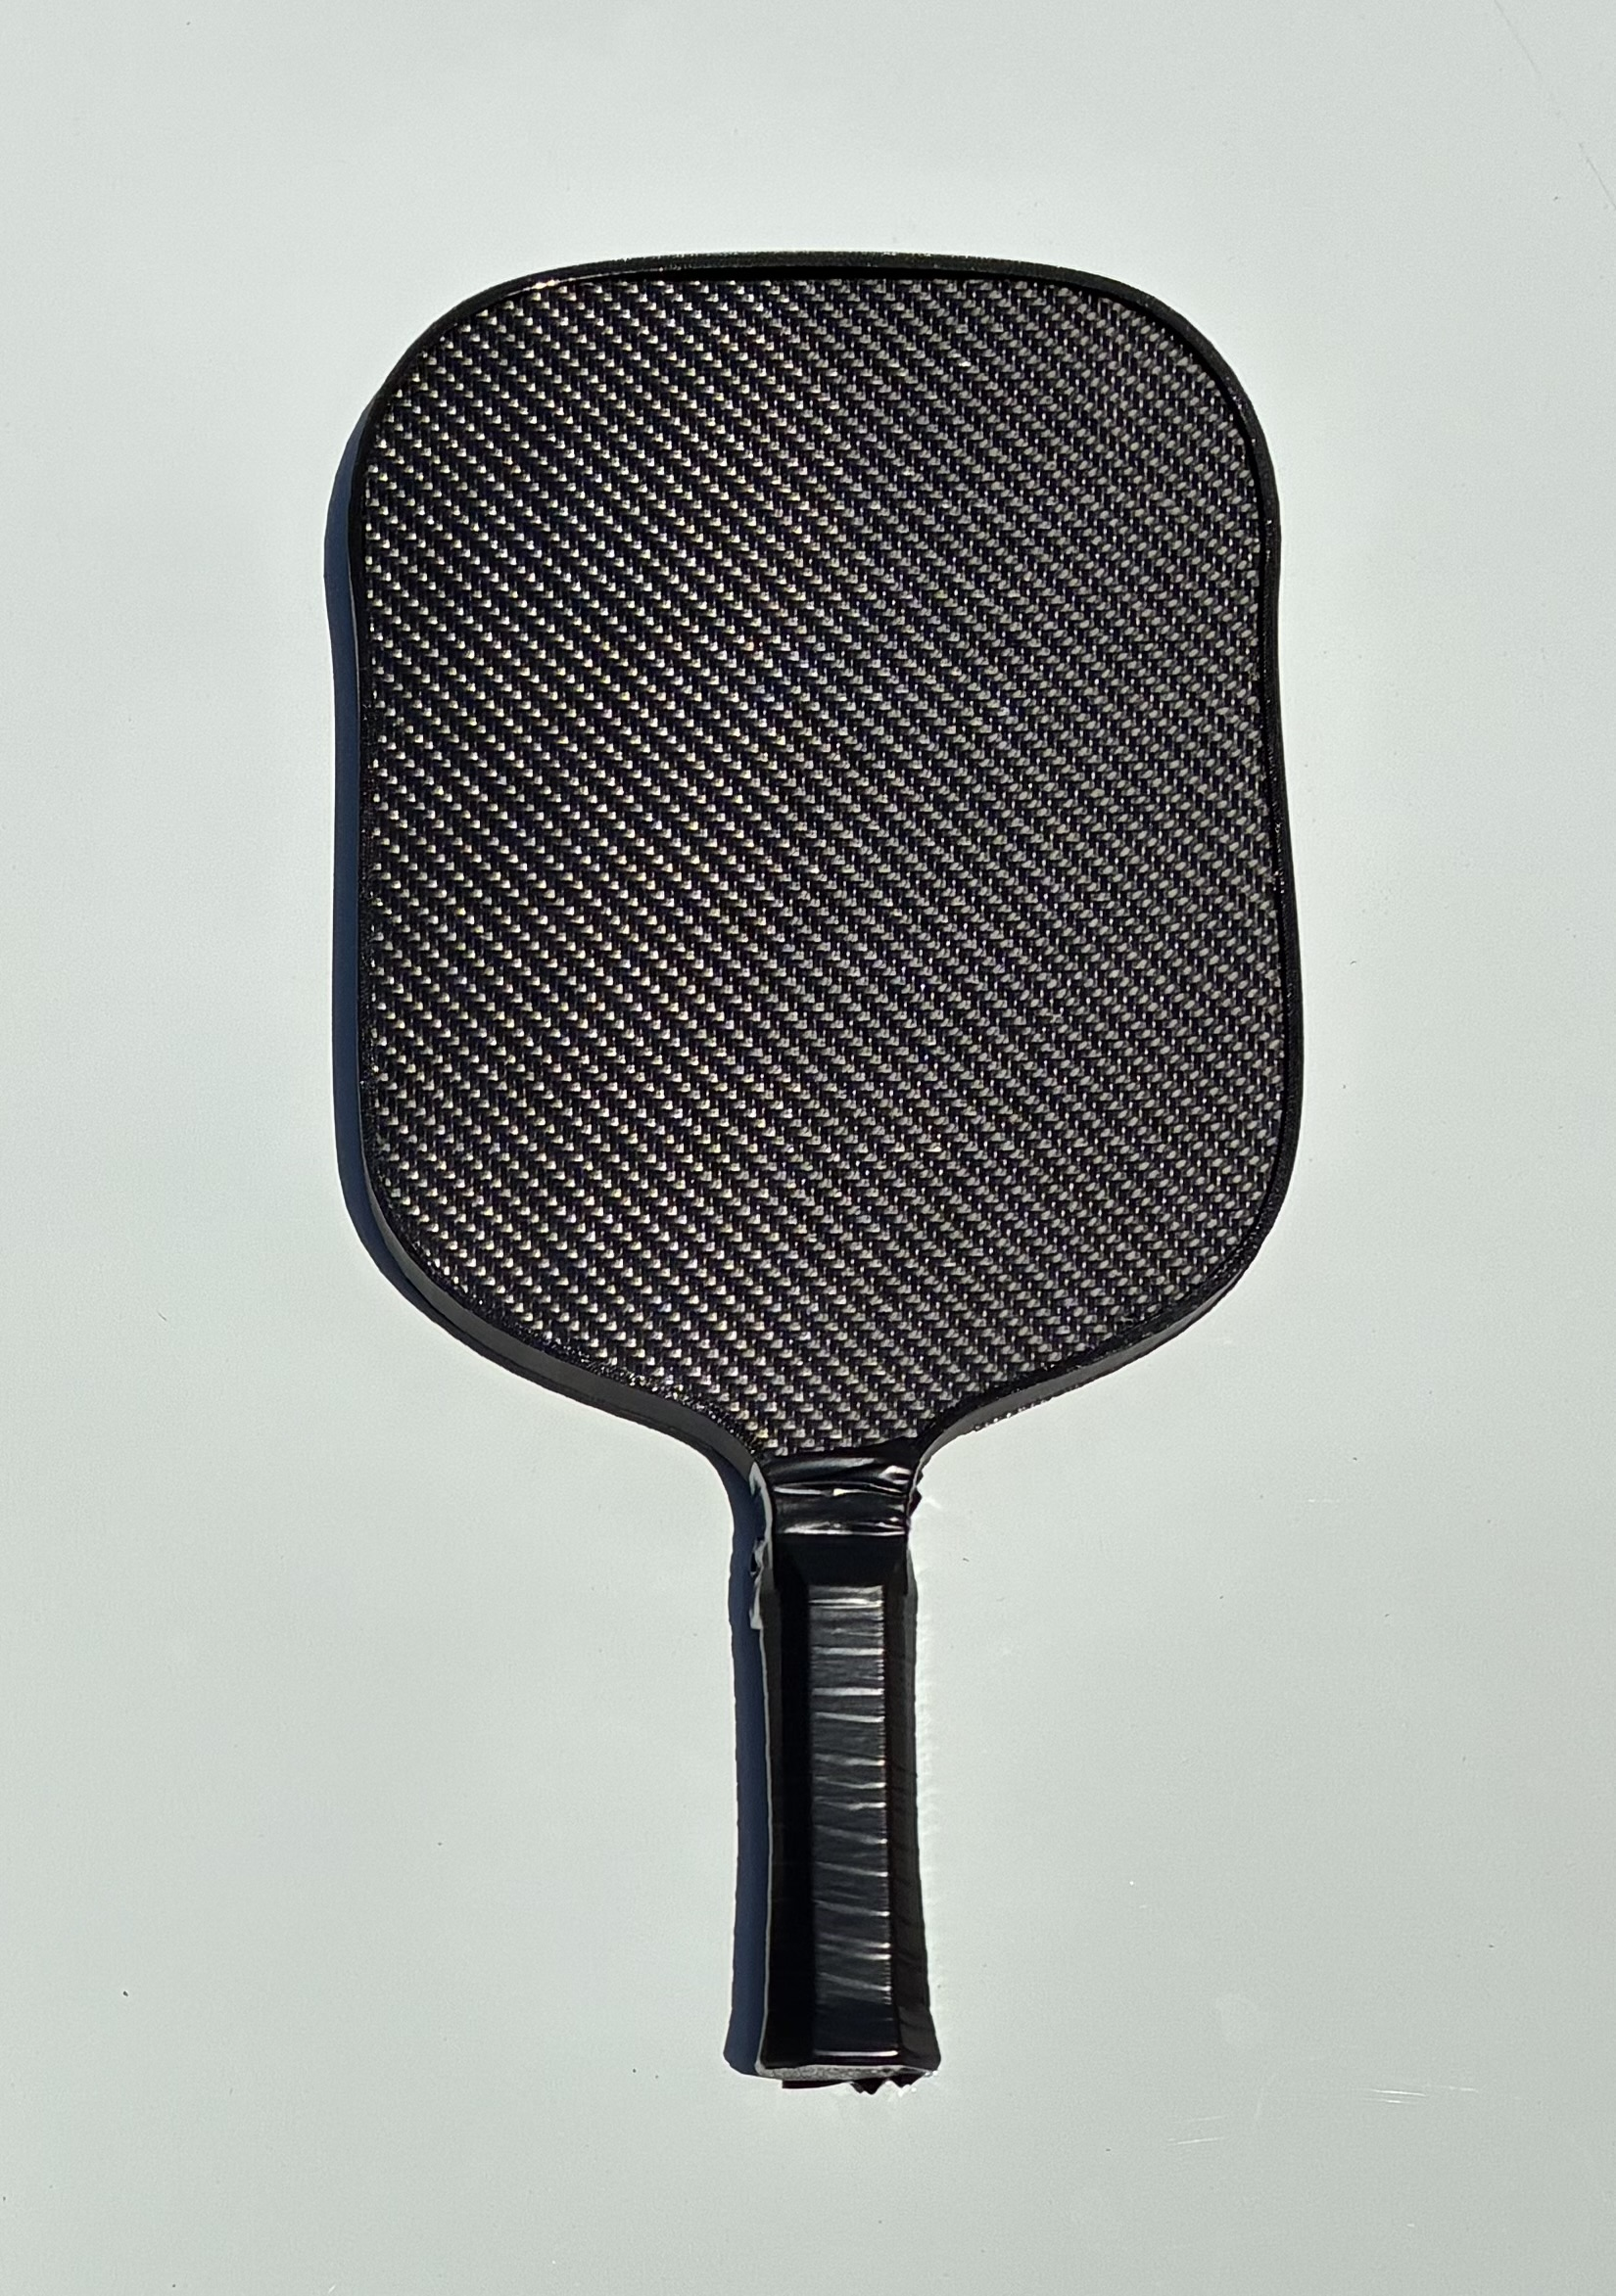
\includegraphics[
        width=3.72in,
        height=3.18in,
        keepaspectratio
    ]{full_assy}
};

\node[
    anchor=north,
    text=Muted,
    font=\sffamily\fontsize{6.9}{7.5}\selectfont
]
at ($(current page.north west)+(1.60in,-4.86in)$)
{Completed solo-built paddle assembly};

% ============================================================
% TOP CENTER — PROJECT OVERVIEW
% ============================================================

\fill[SoftGold,rounded corners=5pt]
    ($(current page.north west)+(2.95in,-1.62in)$)
    rectangle
    ($(current page.north west)+(5.53in,-4.86in)$);

\fill[PolyGold]
    ($(current page.north west)+(2.95in,-1.62in)$)
    rectangle
    ($(current page.north west)+(3.05in,-4.86in)$);

\node[
    anchor=north west,
    text=DeepGreen,
    font=\sffamily\bfseries\fontsize{8.0}{8.7}\selectfont
]
at ($(current page.north west)+(3.23in,-1.79in)$)
{PROJECT OVERVIEW};

\node[
    anchor=north west,
    align=left,
    text width=2.02in,
    text=Ink,
    font=\fontsize{7.05}{8.35}\selectfont
]
at ($(current page.north west)+(3.23in,-2.07in)$)
{
Independently designed and manufactured a lightweight prepreg
carbon-fiber pickleball paddle using a half-inch honeycomb
sandwich core, vacuum-bag consolidation, precision waterjet
trimming, and custom TPU and PLA components.

\vspace{5pt}

The project emphasized lightweight sandwich-composite design, repeatable manufacturing methods, dimensional accuracy, and the integration of custom 3D-printed TPU and PLA components into the final assembly.
};

\node[
    anchor=south west,
    align=left,
    text width=2.02in,
    text=PolyGold,
    font=\sffamily\bfseries\fontsize{6.65}{7.35}\selectfont
]
at ($(current page.north west)+(3.23in,-4.74in)$)
{
SOLE DESIGNER\\[2pt]
COMPOSITE FABRICATOR\\[2pt]
MANUFACTURING ENGINEER
};

% ============================================================
% TOP RIGHT — LAMINATE GRAPHIC
% ============================================================

\node[
    anchor=north west,
    inner sep=2.5pt,
    draw=DeepGreen,
    line width=0.65pt,
    rounded corners=5pt
]
at ($(current page.north west)+(5.71in,-1.62in)$)
{
    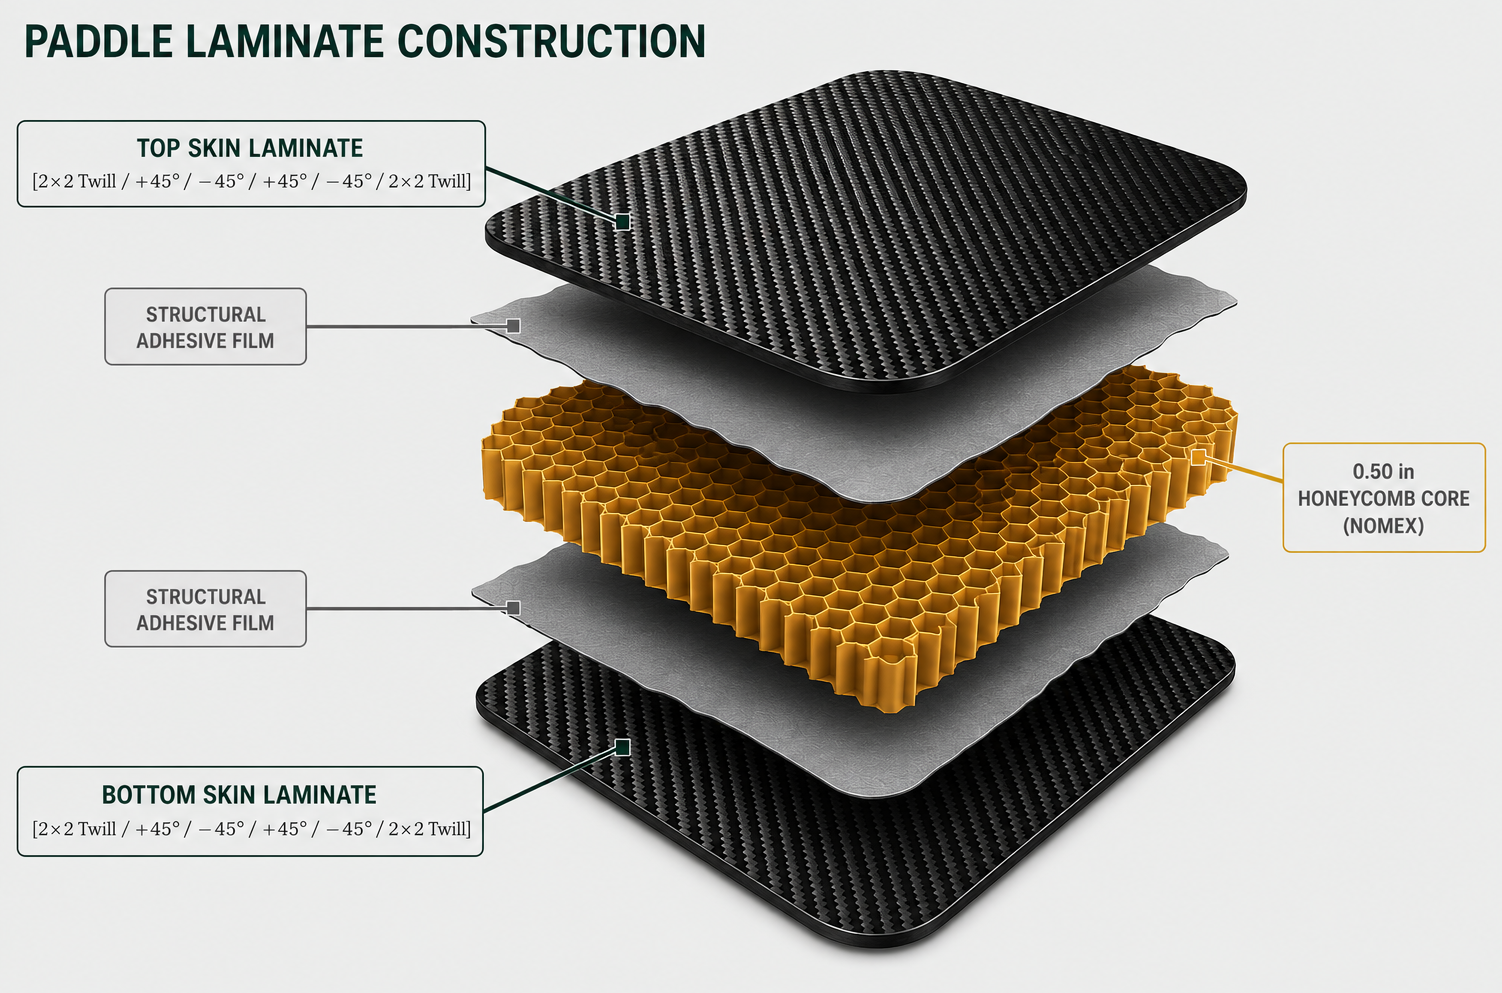
\includegraphics[
        width=4.80in,
        keepaspectratio
    ]{LAMINATE}
};

% ============================================================
% BOTTOM LEFT — SUPPORTING IMAGES
% ============================================================

\node[
    anchor=center,
    inner sep=3pt,
    draw=RuleGray,
    line width=0.55pt,
    rounded corners=4pt
]
at ($(current page.north west)+(1.12in,-5.98in)$)
{
    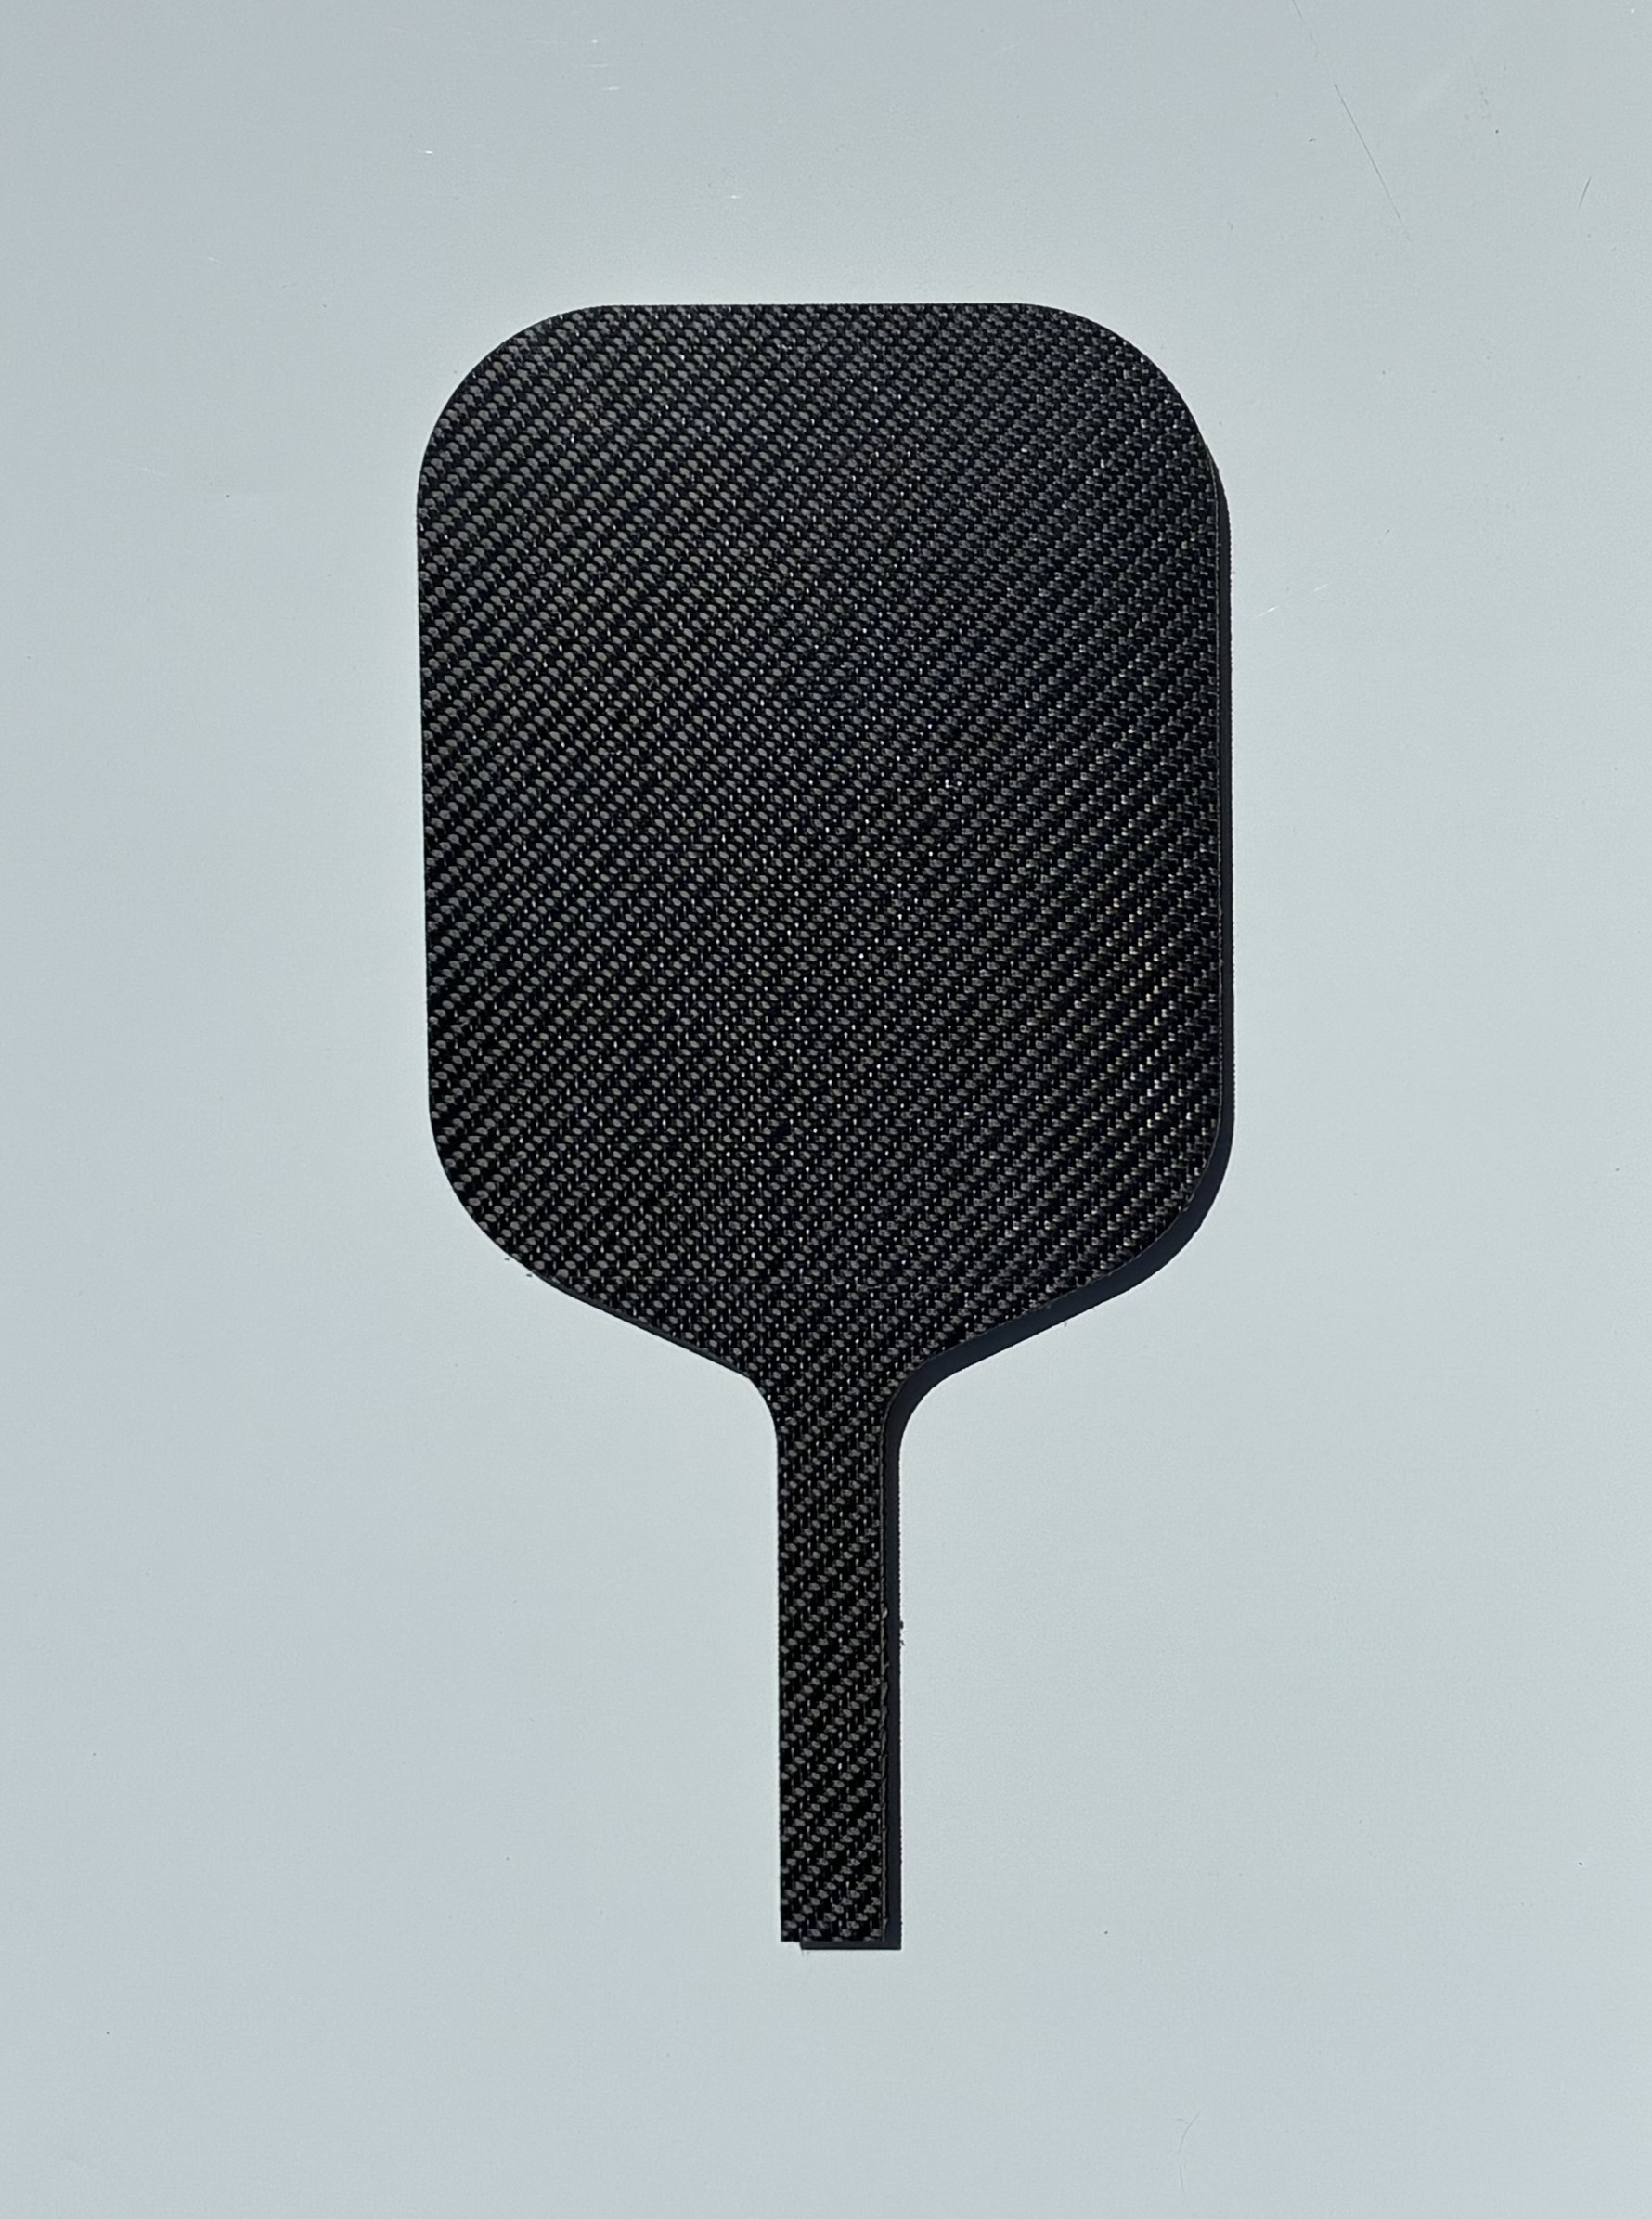
\includegraphics[
        width=1.30in,
        height=1.78in,
        keepaspectratio
    ]{front_view}
};

\node[
    anchor=center,
    inner sep=3pt,
    draw=RuleGray,
    line width=0.55pt,
    rounded corners=4pt
]
at ($(current page.north west)+(2.72in,-5.98in)$)
{
    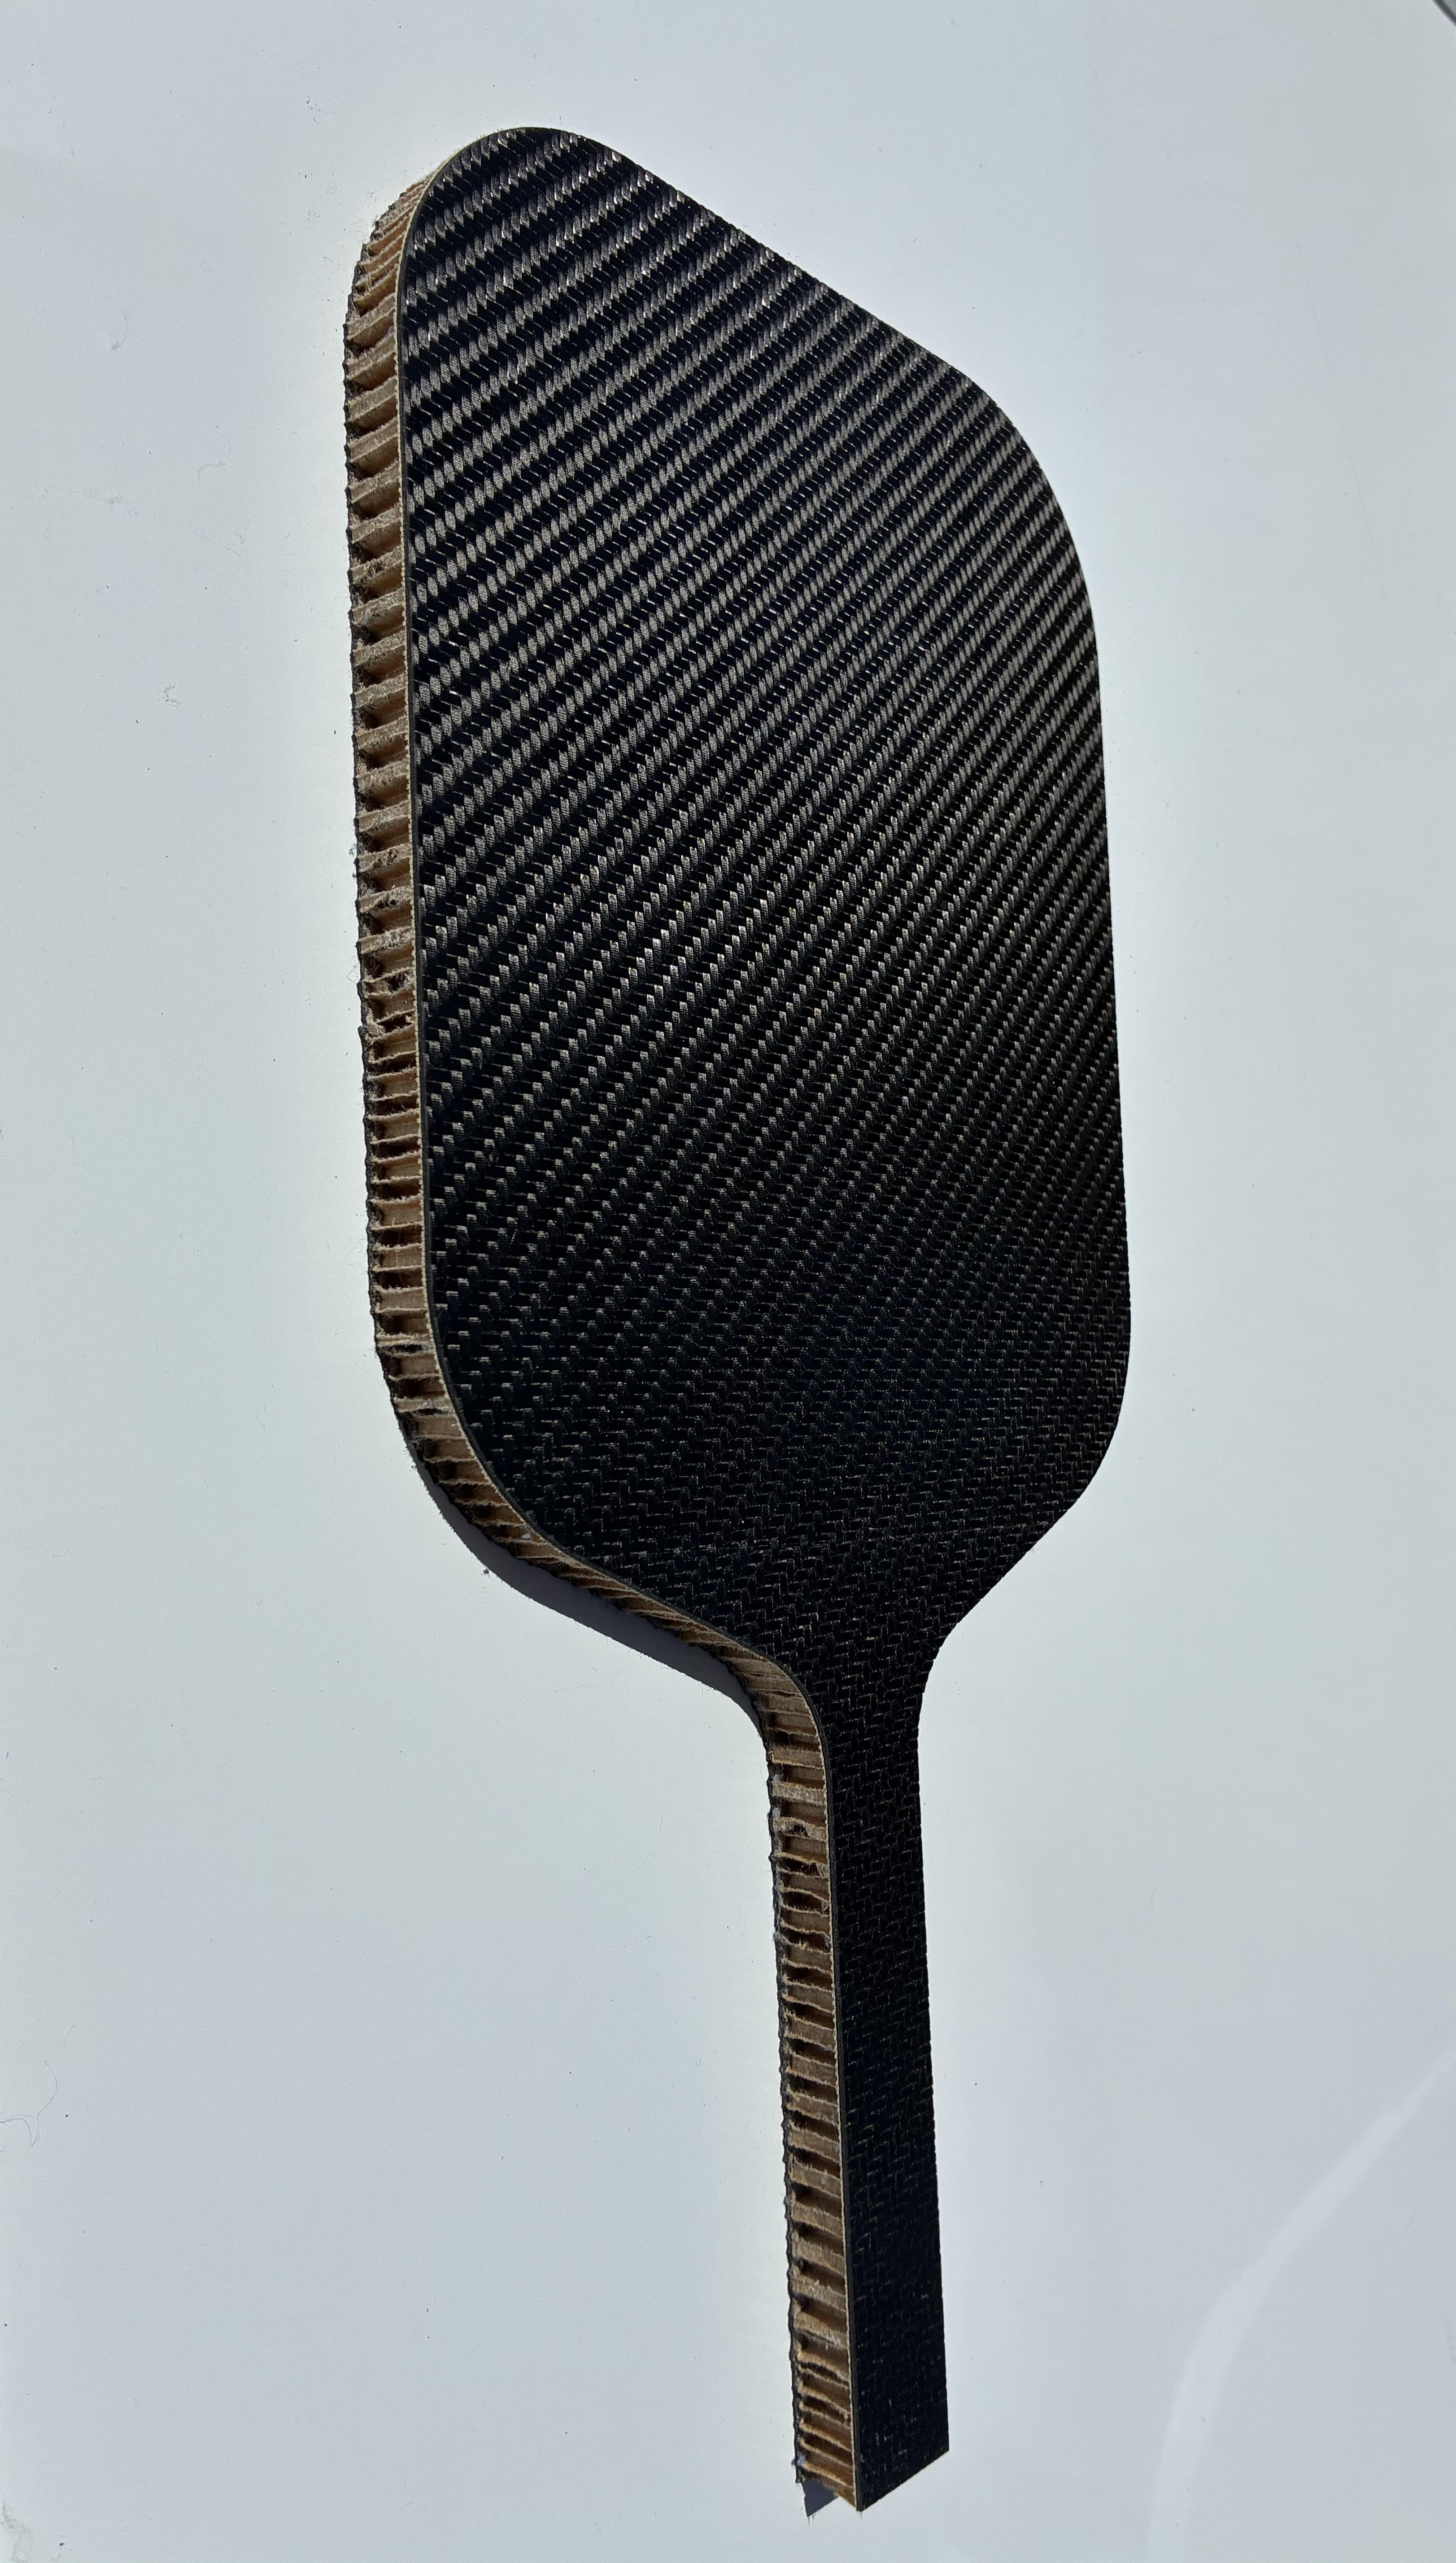
\includegraphics[
        width=1.30in,
        height=1.78in,
        keepaspectratio
    ]{side_core_view}
};

\node[
    anchor=center,
    inner sep=3pt,
    draw=RuleGray,
    line width=0.55pt,
    rounded corners=4pt
]
at ($(current page.north west)+(4.32in,-5.98in)$)
{
    \includegraphics[
        angle=-90,
        origin=c,
        width=1.30in,
        height=1.78in,
        keepaspectratio
    ]{waterjet}
};

\node[
    anchor=north,
    align=center,
    text width=1.38in,
    text=Muted,
    font=\sffamily\fontsize{6.5}{7.1}\selectfont
]
at ($(current page.north west)+(1.12in,-7.00in)$)
{Front view};

\node[
    anchor=north,
    align=center,
    text width=1.38in,
    text=Muted,
    font=\sffamily\fontsize{6.5}{7.1}\selectfont
]
at ($(current page.north west)+(2.72in,-7.00in)$)
{Core and edge profile};

\node[
    anchor=north,
    align=center,
    text width=1.38in,
    text=Muted,
    font=\sffamily\fontsize{6.5}{7.1}\selectfont
]
at ($(current page.north west)+(4.32in,-7.00in)$)
{Waterjet cutting setup};

% ============================================================
% BOTTOM RIGHT — MANUFACTURING HIGHLIGHTS
% ============================================================

\fill[SoftGreen,rounded corners=5pt]
    ($(current page.north west)+(5.18in,-5.05in)$)
    rectangle
    ($(current page.north east)+(-0.42in,-7.18in)$);

\draw[RuleGray,line width=0.55pt,rounded corners=5pt]
    ($(current page.north west)+(5.18in,-5.05in)$)
    rectangle
    ($(current page.north east)+(-0.42in,-7.18in)$);

\node[
    anchor=north west,
    text=DeepGreen,
    font=\sffamily\bfseries\fontsize{7.9}{8.6}\selectfont
]
at ($(current page.north west)+(5.44in,-5.20in)$)
{MANUFACTURING HIGHLIGHTS};

\node[
    anchor=north west,
    align=left,
    text width=5.05in,
    text=Ink,
    font=\fontsize{6.72}{7.82}\selectfont
]
at ($(current page.north west)+(5.44in,-5.49in)$)
{
\textbf{Consolidation.}
Vacuum bagging and distributed weight pressure maintained intimate contact
throughout the prepreg sandwich layup.\\[2.4pt]
\textbf{Surface quality.}
A scarce PTFE release film produced an unusually consistent matte finish
with a subtle sheen and minimal post-processing.\\[2.4pt]
\textbf{Waterjet stability.}
Perimeter weights restrained the cured stock against jet-induced lifting
and rotational moments during cutting.\\[2.4pt]
\textbf{Final assembly.}
A printed TPU edge band protected the carbon perimeter, while the PLA handle
used clearance cutouts to accommodate future stock-thickness and cutting variation.
};

% ============================================================
% RESOURCE LINK
% ============================================================

\node[
    anchor=north,
    align=center,
    text=DeepGreen,
    font=\sffamily\bfseries\fontsize{7.0}{7.6}\selectfont
]
at ($(current page.north)+(0,-7.42in)$)
{\href{\PaddleWaterjetVideo}
{\faPlayCircle\ WATERJET PICKLEBALL PADDLE DEMONSTRATION}};

% ============================================================
% FOOTER
% ============================================================

\node[
    anchor=south west,
    text=white,
    font=\sffamily\bfseries\fontsize{7.1}{7.7}\selectfont
]
at ($(current page.south west)+(0.42in,0.17in)$)
{\hyperlink{toro-results}{\faArrowLeft\ TORO COVER}};

\node[
    anchor=south,
    text=white,
    font=\sffamily\fontsize{7.0}{7.6}\selectfont
]
at ($(current page.south)+(0,0.17in)$)
{PICKLEBALL PADDLE \hspace{6pt} 1 / 1};

\node[
    anchor=south east,
    text=white,
    font=\sffamily\bfseries\fontsize{7.1}{7.7}\selectfont
]
at ($(current page.south east)+(-0.42in,0.17in)$)
{NEXT PROJECT \faArrowRight};

\end{tikzpicture}
%% ============================================================
% CARBON FIBER I-BEAM — SINGLE-PAGE PORTFOLIO CASE STUDY
% 01 Composites / Project 03
%
% IMPORTANT:
% 1. This file must NOT contain \documentclass, \begin{document},
%    or \end{document}.
% 2. In main.tex, place \input{ibeam_one_page} before \end{document}.
% 3. This script assumes the main portfolio preamble already defines:
%       DeepGreen, PolyGold, SoftGold, SoftGreen,
%       RuleGray, Muted, Ink
%    and loads tikz, graphicx, hyperref, and fontawesome5.
% 4. Upload these image files to Overleaf with the same names:
%       front view assembly graphic.png
%       Distributed weight with bolts.jpg
%       Stress Analysis on Generic CAD model.png
%       Beam Fiulure Delamination and cracking.jpeg
%       Three Point Bend Test.JPG
% ============================================================

\providecommand{\IBeamCompetitionGuidelines}
{https://drive.google.com/file/d/16S6MPVWWzPNKjXWVGKEySAi9i1f1BZYn/view?usp=sharing}

\providecommand{\IBeamBendTestVideo}
{https://drive.google.com/file/d/1LK_-pyK_y-a_4gDTiasz4uLUi95nAfrO/view?usp=drive_link}

\clearpage
\thispagestyle{empty}
\hypertarget{ibeam}{}
\null

\begin{tikzpicture}[remember picture,overlay]

% ============================================================
% BACKGROUND AND PAGE BARS
% ============================================================

\fill[white]
    (current page.south west)
    rectangle
    (current page.north east);

\fill[DeepGreen]
    (current page.north west)
    rectangle
    ($(current page.north east)+(0,-0.095in)$);

\fill[PolyGold]
    ($(current page.north west)+(0,-0.095in)$)
    rectangle
    ($(current page.north east)+(0,-0.14in)$);

\fill[DeepGreen]
    (current page.south west)
    rectangle
    ($(current page.south east)+(0,0.36in)$);

\fill[PolyGold]
    ($(current page.south west)+(0,0.36in)$)
    rectangle
    ($(current page.south east)+(0,0.405in)$);

% ============================================================
% HEADER
% ============================================================

\node[
    anchor=north west,
    text=PolyGold,
    font=\sffamily\bfseries\fontsize{8.1}{8.7}\selectfont
]
at ($(current page.north west)+(0.42in,-0.39in)$)
{01 COMPOSITES \hspace{5pt}/\hspace{5pt} PROJECT 03};

\node[
    anchor=north west,
    text=DeepGreen,
    font=\bfseries\fontsize{22.3}{23.3}\selectfont
]
at ($(current page.north west)+(0.40in,-0.67in)$)
{CARBON FIBER I-BEAM DESIGN \& TESTING};

\node[
    anchor=north west,
    text=Muted,
    font=\sffamily\fontsize{8.25}{9.0}\selectfont
]
at ($(current page.north west)+(0.42in,-1.12in)$)
{Cal Poly Composites Laboratory \hspace{7pt}\textbullet\hspace{7pt}
Individual Project \hspace{7pt}\textbullet\hspace{7pt}
Winter 2026 \hspace{7pt}\textbullet\hspace{7pt}
San Luis Obispo, California};

\fill[PolyGold]
    ($(current page.north west)+(0.42in,-1.36in)$)
    rectangle
    ($(current page.north west)+(6.10in,-1.315in)$);


% ============================================================
% TOP LEFT — ASSEMBLY ARCHITECTURE
% ============================================================

\node[
    anchor=north west,
    inner sep=2.6pt,
    draw=DeepGreen,
    line width=0.68pt,
    rounded corners=5pt
]
at ($(current page.north west)+(0.42in,-1.58in)$)
{
    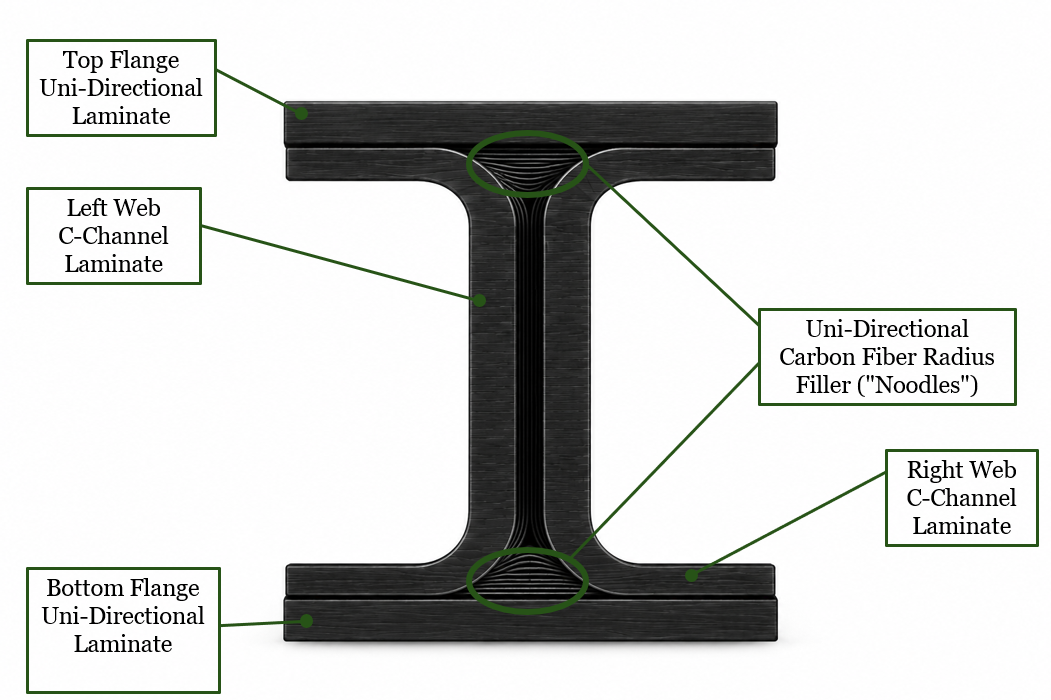
\includegraphics[
        width=3.55in,
        height=2.45in,
        keepaspectratio
    ]{front view assembly graphic.png}
};

\node[
    anchor=north,
    align=center,
    inner sep=0pt,
    text width=3.42in,
    text=Muted,
    font=\sffamily\fontsize{6.35}{7.05}\selectfont
]
at ($(current page.north west)+(2.195in,-4.12in)$)
{Four-piece laminate architecture with top and bottom flange laminates, paired C-channels, and longitudinal radius fillers};

% ============================================================
% TOP CENTER — PROJECT OVERVIEW + C-CHANNEL LAYUP
% ============================================================

\fill[SoftGold,rounded corners=5pt]
    ($(current page.north west)+(4.18in,-1.58in)$)
    rectangle
    ($(current page.north west)+(7.42in,-4.20in)$);

\fill[PolyGold]
    ($(current page.north west)+(4.18in,-1.58in)$)
    rectangle
    ($(current page.north west)+(4.28in,-4.20in)$);

\node[
    anchor=north west,
    text=DeepGreen,
    font=\sffamily\bfseries\fontsize{8.0}{8.7}\selectfont
]
at ($(current page.north west)+(4.48in,-1.76in)$)
{PROJECT OVERVIEW};

\node[
    anchor=north west,
    align=left,
    text width=2.64in,
    text=Ink,
    font=\fontsize{6.40}{7.45}\selectfont
]
at ($(current page.north west)+(4.48in,-2.04in)$)
{
A 24-inch carbon-fiber I-beam was manufactured from two molded
C-channel laminates, separate top and bottom flange laminates,
and longitudinal unidirectional radius fillers. The completed
684 g specimen sustained 28.2 kN (6,340 lbf) in three-point bending.\\[3pt]
\textbf{C-channel layup.}
Each channel used the same 12-ply sequence:
\mbox{$[+45/-45/0/+45/-45/0/0/-45/+45/0/-45/+45]$}.
The layup was completed twice, once for each channel.\\[3pt]
\textbf{Flange layups.}
Top flange: \mbox{$[90/0_6/90/0_6]$}. Bottom flange:
\mbox{$[90/0_6]$}, where $0_6$ denotes six consecutive 0-degree plies.
};

\node[
    anchor=south west,
    text=PolyGold,
    font=\sffamily\bfseries\fontsize{6.45}{7.1}\selectfont
]
at ($(current page.north west)+(4.48in,-4.03in)$)
{MASS: 684 g \hspace{8pt}\textbullet\hspace{8pt} PEAK LOAD: 28.2 kN \hspace{8pt}\textbullet\hspace{8pt} LENGTH: 24 in};

% ============================================================
% TOP RIGHT — C-CHANNEL MANUFACTURING
% ============================================================

\node[
    anchor=north west,
    inner sep=2.6pt,
    draw=DeepGreen,
    line width=0.68pt,
    rounded corners=5pt
]
at ($(current page.north west)+(7.62in,-1.58in)$)
{
    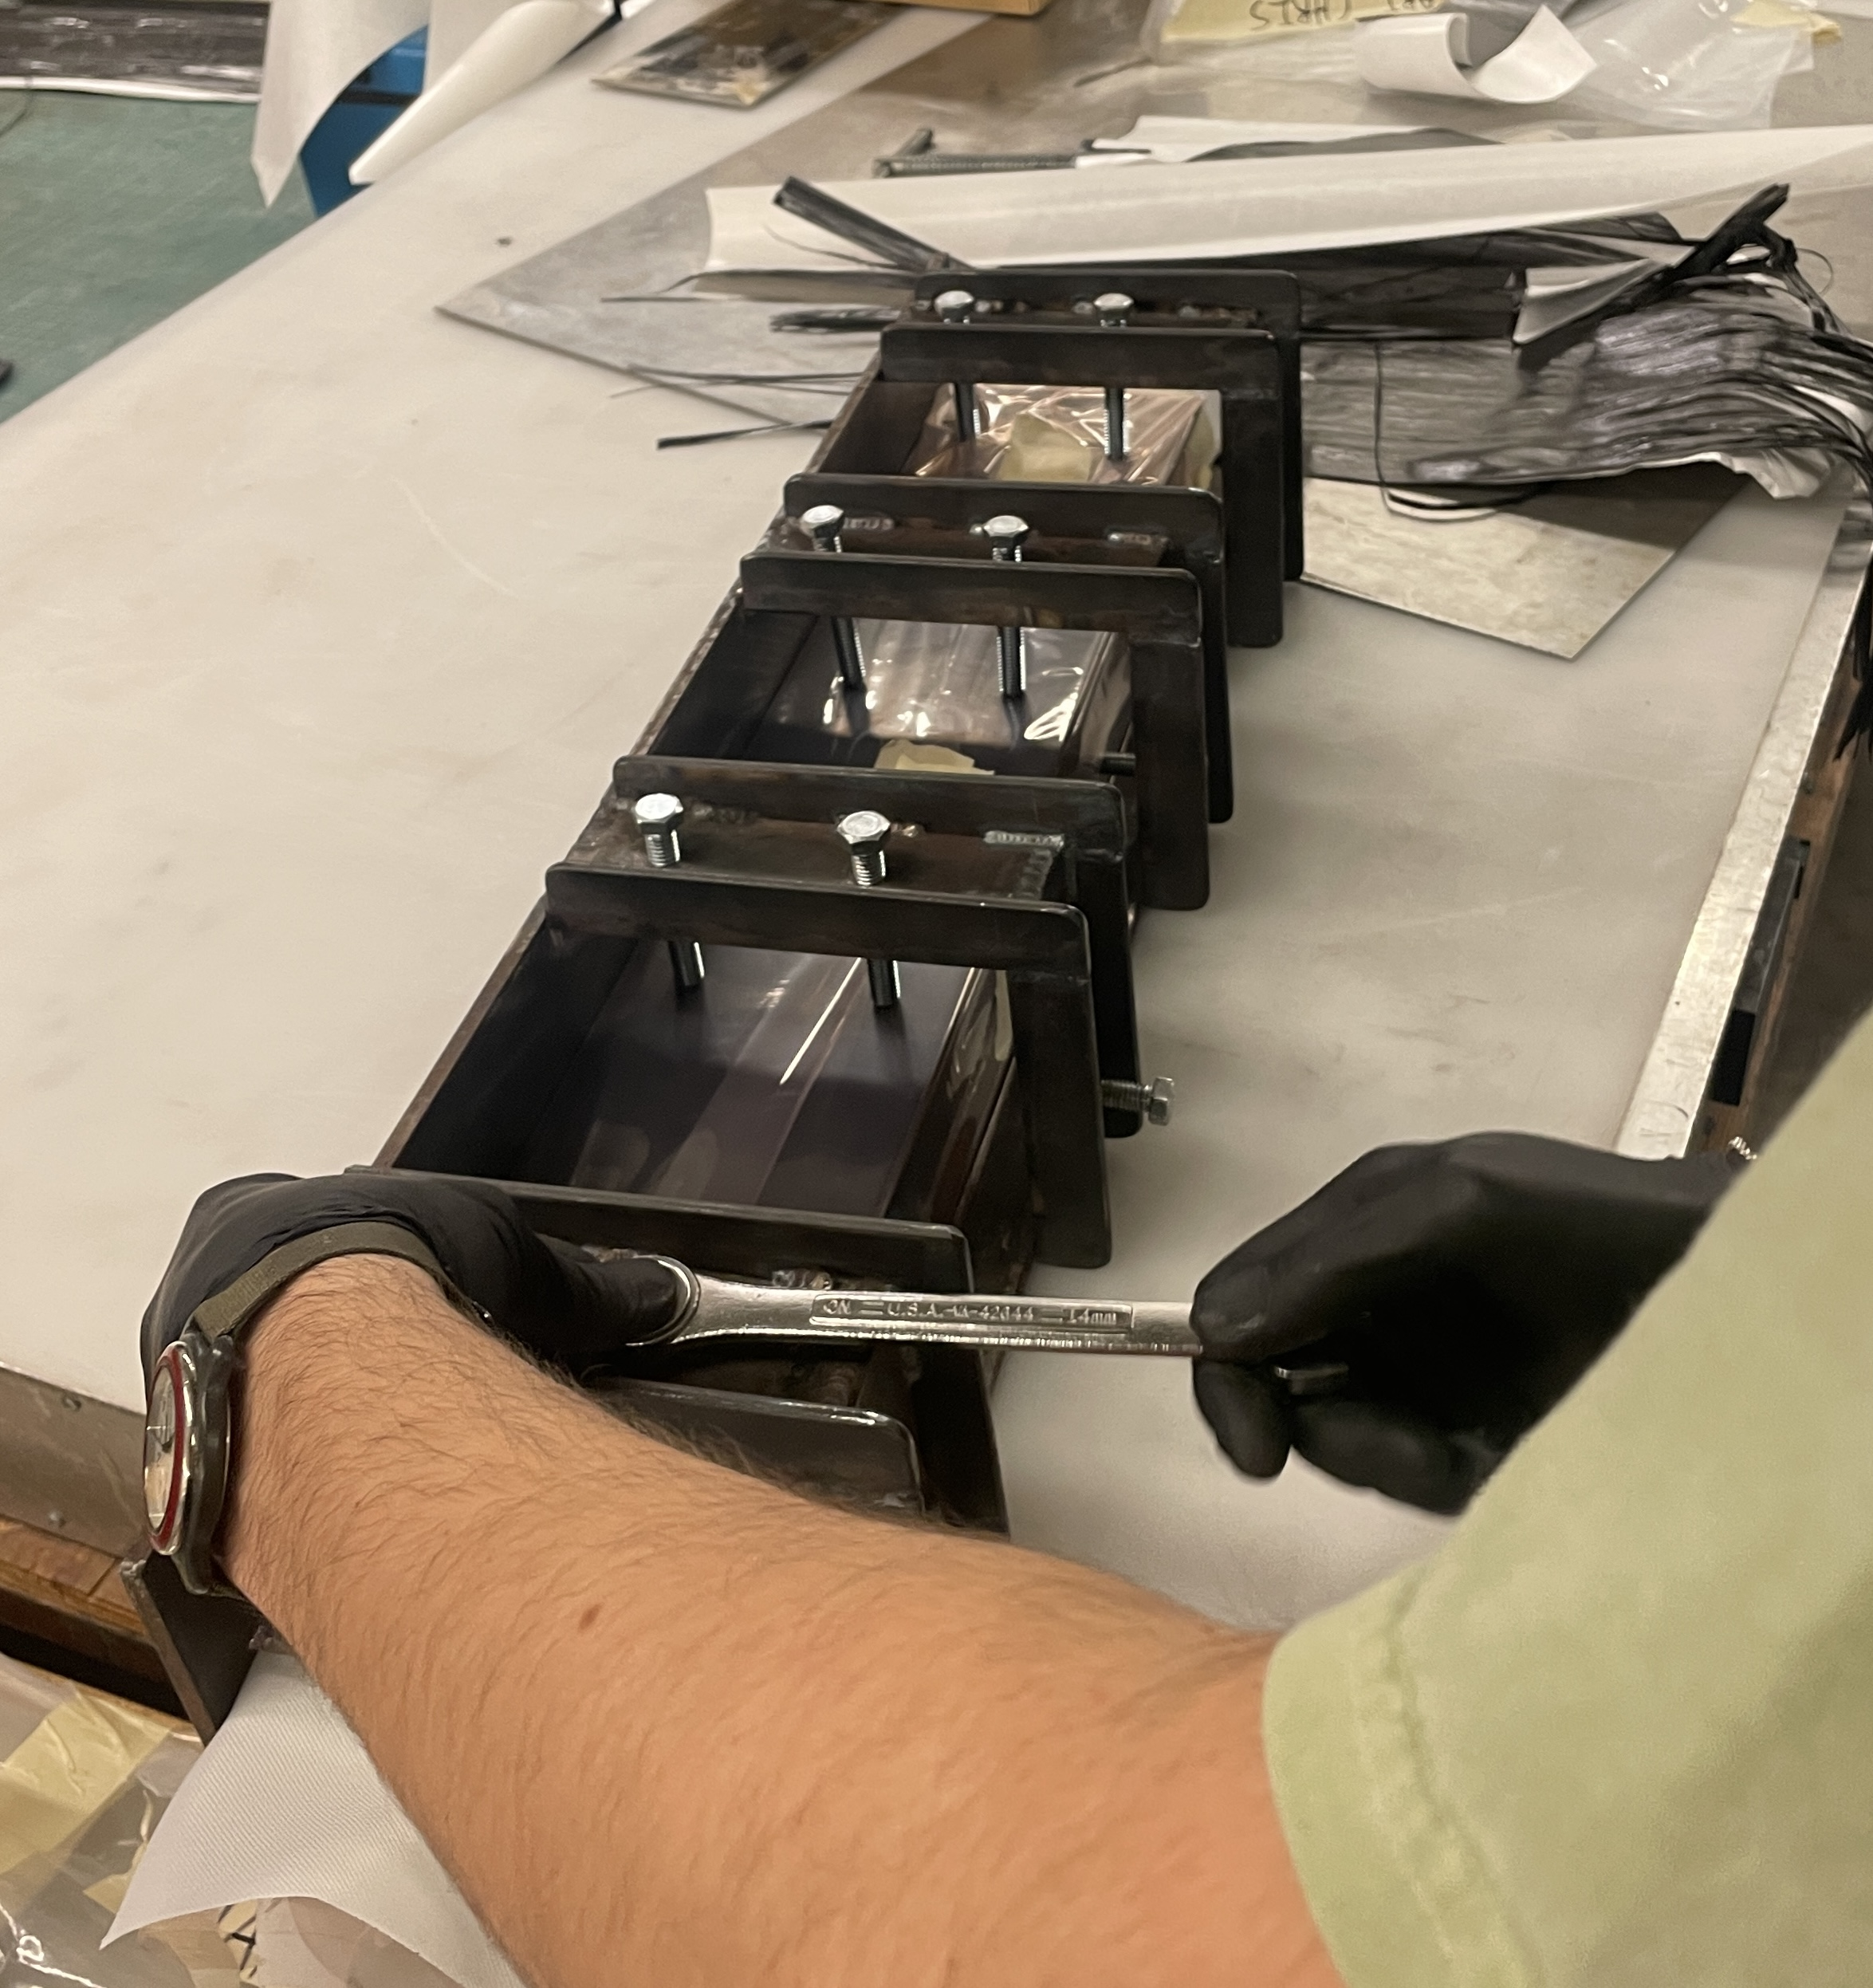
\includegraphics[
        width=3.55in,
        height=2.45in,
        keepaspectratio
    ]{Distributed weight with bolts.jpg}
};

\node[
    anchor=north,
    align=center,
    inner sep=0pt,
    text width=3.42in,
    text=Muted,
    font=\sffamily\fontsize{6.35}{7.05}\selectfont
]
at ($(current page.north west)+(9.395in,-4.12in)$)
{Distributed bolt pressure maintained alignment and consolidated the full beam assembly during cure};

% ============================================================
% CENTER ROW — MODEL, TEST, AND OBSERVED FAILURE
% ============================================================

\node[
    anchor=north west,
    inner sep=2.4pt,
    draw=RuleGray,
    line width=0.55pt,
    rounded corners=4pt
]
at ($(current page.north west)+(0.42in,-4.43in)$)
{
    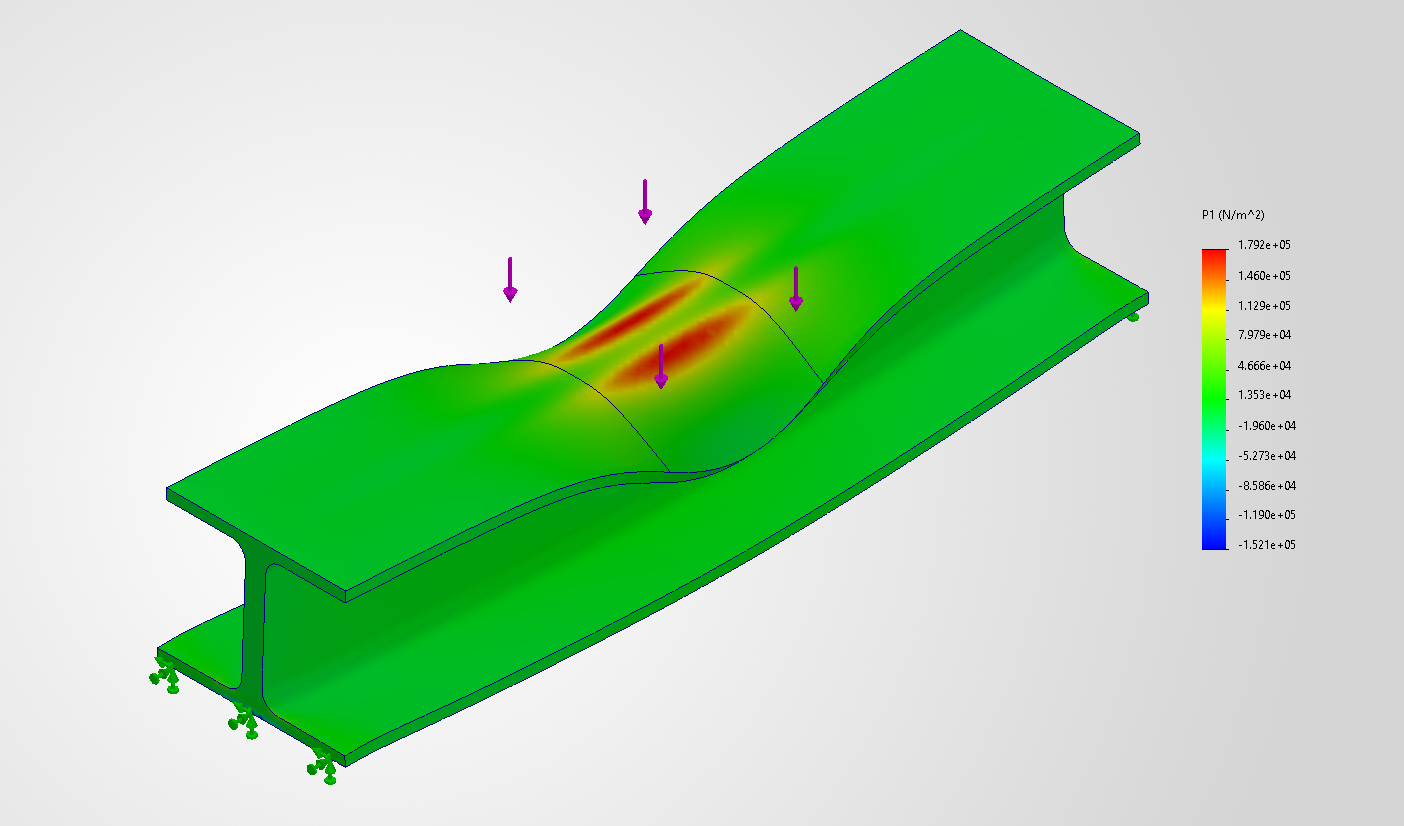
\includegraphics[
        width=3.33in,
        height=1.62in,
        keepaspectratio
    ]{Stress Analysis on Generic CAD model.png}
};

\node[
    anchor=north,
    align=center,
    inner sep=0pt,
    text width=3.20in,
    text=Muted,
    font=\sffamily\fontsize{6.20}{6.85}\selectfont
]
at ($(current page.north west)+(2.085in,-6.14in)$)
{Generic FEA predicted peak compressive stress beneath the center loading shoe};

\node[
    anchor=north west,
    inner sep=2.4pt,
    draw=RuleGray,
    line width=0.55pt,
    rounded corners=4pt
]
at ($(current page.north west)+(3.92in,-4.43in)$)
{
    \includegraphics[
        angle=180,
        origin=c,
        width=3.18in,
        height=1.62in,
        keepaspectratio
    ]{Three Point Bend Test.JPG}
};

\node[
    anchor=north,
    align=center,
    inner sep=0pt,
    text width=3.05in,
    text=Muted,
    font=\sffamily\fontsize{6.20}{6.85}\selectfont
]
at ($(current page.north west)+(5.510in,-6.14in)$)
{Experimental three-point bend test on the completed I-beam specimen};

\node[
    anchor=north west,
    inner sep=2.4pt,
    draw=RuleGray,
    line width=0.55pt,
    rounded corners=4pt
]
at ($(current page.north west)+(7.28in,-4.43in)$)
{
    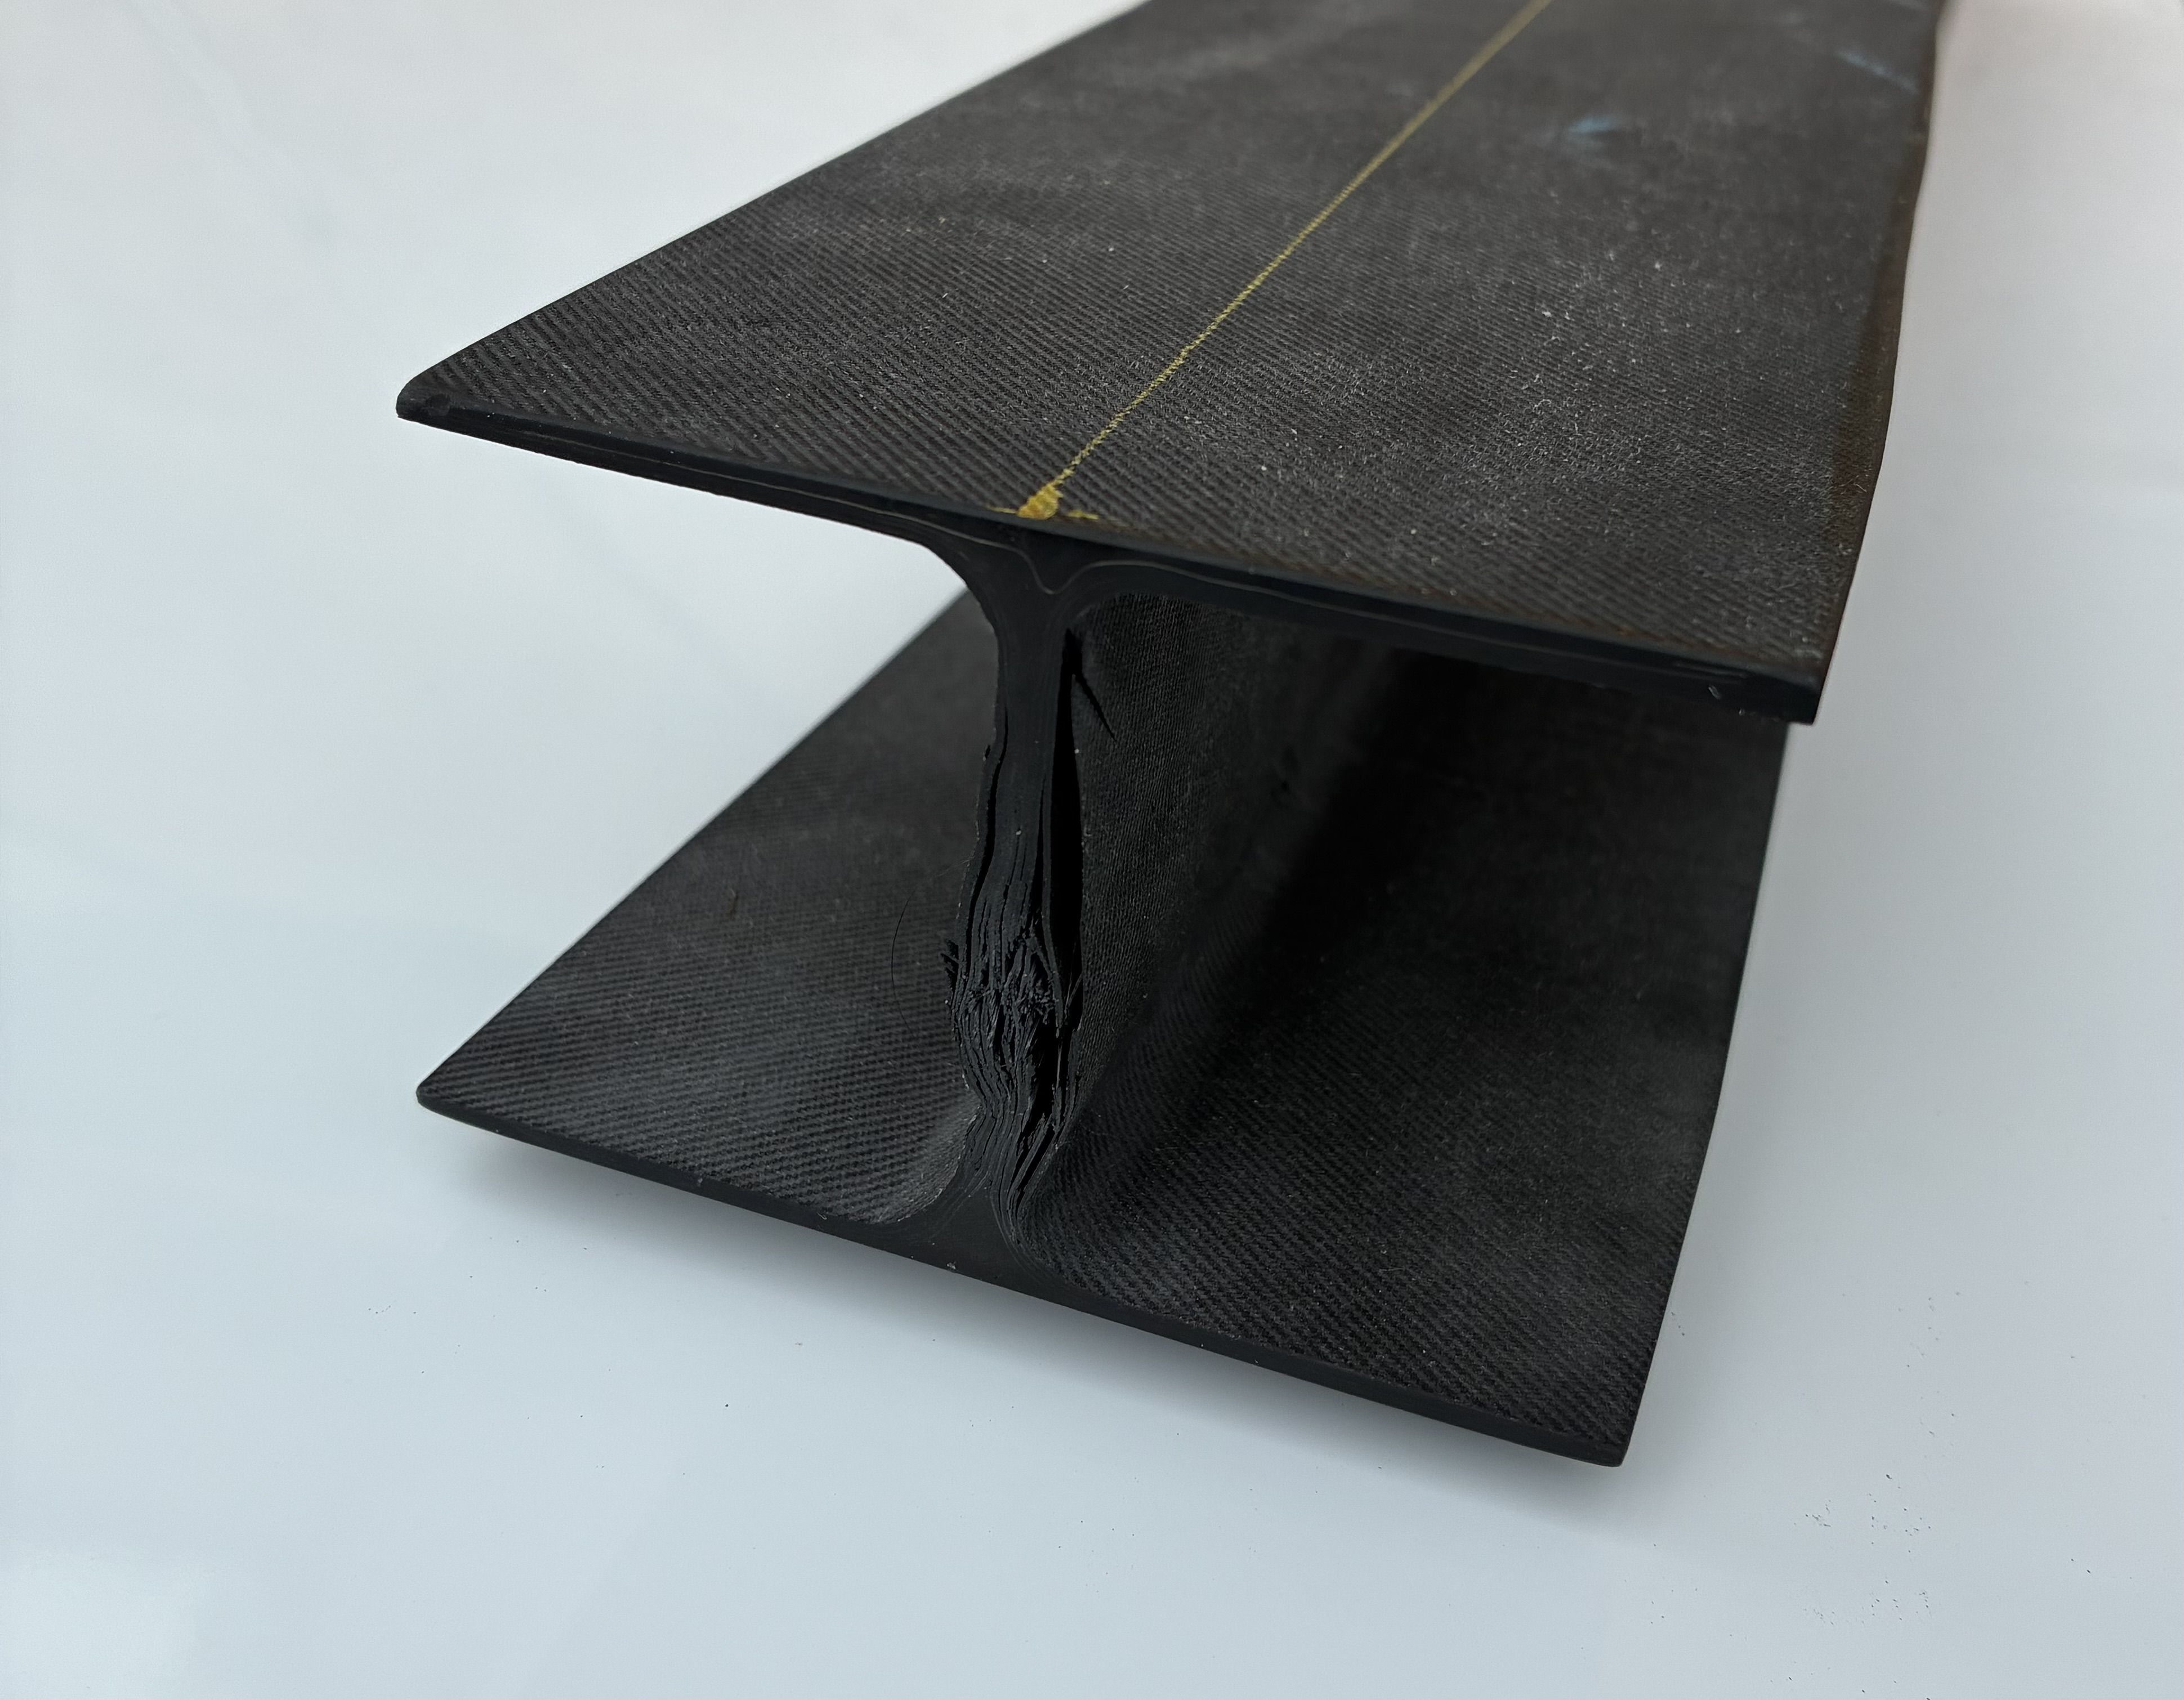
\includegraphics[
        width=3.65in,
        height=1.62in,
        keepaspectratio
    ]{Beam Fiulure Delamination and cracking.jpeg}
};

\node[
    anchor=north,
    align=center,
    inner sep=0pt,
    text width=3.50in,
    text=Muted,
    font=\sffamily\fontsize{6.20}{6.85}\selectfont
]
at ($(current page.north west)+(9.105in,-6.14in)$)
{Observed edge failure with delamination and longitudinal crack propagation};

% ============================================================
% BOTTOM LEFT — MANUFACTURING PROCESS
% ============================================================

\fill[SoftGreen,rounded corners=5pt]
    ($(current page.north west)+(0.42in,-6.43in)$)
    rectangle
    ($(current page.north west)+(5.30in,-7.18in)$);

\draw[RuleGray,line width=0.55pt,rounded corners=5pt]
    ($(current page.north west)+(0.42in,-6.43in)$)
    rectangle
    ($(current page.north west)+(5.30in,-7.18in)$);

\node[
    anchor=north west,
    text=DeepGreen,
    font=\sffamily\bfseries\fontsize{7.65}{8.35}\selectfont
]
at ($(current page.north west)+(0.66in,-6.57in)$)
{MANUFACTURING APPROACH};

\node[
    anchor=north west,
    align=left,
    text width=4.38in,
    text=Ink,
    font=\fontsize{6.20}{7.15}\selectfont
]
at ($(current page.north west)+(0.66in,-6.82in)$)
{
The separately molded channels were aligned with longitudinal carbon-fiber
``noodles'' filling the radius-induced flange voids. Top and bottom flanges
were then installed, and the full assembly was consolidated in a custom
steel fixture using distributed bolt pressure along the beam length.
};

% ============================================================
% BOTTOM RIGHT — FAILURE ANALYSIS AND NEXT ITERATION
% ============================================================

\fill[SoftGold,rounded corners=5pt]
    ($(current page.north west)+(5.52in,-6.43in)$)
    rectangle
    ($(current page.north east)+(-0.42in,-7.18in)$);

\fill[PolyGold]
    ($(current page.north west)+(5.52in,-6.43in)$)
    rectangle
    ($(current page.north west)+(5.62in,-7.18in)$);

\node[
    anchor=north west,
    text=DeepGreen,
    font=\sffamily\bfseries\fontsize{7.65}{8.35}\selectfont
]
at ($(current page.north west)+(5.82in,-6.57in)$)
{FAILURE ANALYSIS AND NEXT ITERATION};

\node[
    anchor=north west,
    align=left,
    text width=4.72in,
    text=Ink,
    font=\fontsize{6.14}{7.08}\selectfont
]
at ($(current page.north west)+(5.82in,-6.82in)$)
{
The model suggested a center-span compression failure, but the physical beam
failed near its edge. This mismatch indicates that local consolidation defects
likely enabled premature delamination. A future build should use staged vacuum
debulking after each ply group rather than relying only on manual rolling before
final fixture consolidation.
};

% ============================================================
% RESOURCE LINKS
% ============================================================

\node[
    anchor=north,
    align=center,
    text=DeepGreen,
    font=\sffamily\bfseries\fontsize{6.75}{7.35}\selectfont
]
at ($(current page.north)+(0,-7.43in)$)
{
\href{\IBeamCompetitionGuidelines}{\faFilePdf\ COMPETITION GUIDELINES}
\hspace{16pt}
\href{\IBeamBendTestVideo}{\faPlayCircle\ THREE-POINT BEND TEST VIDEO}
};

% ============================================================
% FOOTER
% ============================================================

\node[
    anchor=south west,
    text=white,
    font=\sffamily\bfseries\fontsize{7.1}{7.7}\selectfont
]
at ($(current page.south west)+(0.42in,0.17in)$)
{\hyperlink{pickleball}{\faArrowLeft\ PICKLEBALL PADDLE}};

\node[
    anchor=south,
    text=white,
    font=\sffamily\fontsize{7.0}{7.6}\selectfont
]
at ($(current page.south)+(0,0.17in)$)
{CARBON FIBER I-BEAM \hspace{6pt} 1 / 1};

\node[
    anchor=south east,
    text=white,
    font=\sffamily\bfseries\fontsize{7.1}{7.7}\selectfont
]
at ($(current page.south east)+(-0.42in,0.17in)$)
{NEXT PROJECT \faArrowRight};

\end{tikzpicture}
% ============================================================
% FIBERGLASS FUSELAGE FEA & THREE-POINT BEND VALIDATION
% SINGLE-PAGE PORTFOLIO CASE STUDY
% 01 Composites / Project 04
%
% IMPORTANT:
% 1. This file must NOT contain \documentclass, \begin{document},
%    or \end{document}.
% 2. In main.tex, place \input{fuselage} before \end{document}.
% 3. This script assumes the main portfolio preamble already defines:
%       DeepGreen, PolyGold, SoftGold, SoftGreen,
%       RuleGray, Muted, Ink
%    and loads tikz, graphicx, hyperref, and fontawesome5.
% 4. Upload these files to Overleaf with the exact same names:
%       Setup & Mesh of FEA.png
%       fuselage 3 point bend test.JPG
%       Countor Plot of Reaction Force.png
%       fuselage data.png
% ============================================================

\providecommand{\FuselageDemoVideo}
{https://drive.google.com/file/d/1xFCbBJXPhVVlnaleRyZeSM8ucD_xWwB2/view?usp=drive_link}

\providecommand{\FuselageFinalReport}
{https://drive.google.com/file/d/1LYRNlwk73l_KRgaSPgzfsYis-9bsuaxX/view?usp=drive_link}

\clearpage
\thispagestyle{empty}
\hypertarget{fuselage}{}
\null

\begin{tikzpicture}[remember picture,overlay]

% ============================================================
% BACKGROUND AND PAGE BARS
% ============================================================

\fill[white]
    (current page.south west)
    rectangle
    (current page.north east);

\fill[DeepGreen]
    (current page.north west)
    rectangle
    ($(current page.north east)+(0,-0.095in)$);

\fill[PolyGold]
    ($(current page.north west)+(0,-0.095in)$)
    rectangle
    ($(current page.north east)+(0,-0.14in)$);

\fill[DeepGreen]
    (current page.south west)
    rectangle
    ($(current page.south east)+(0,0.36in)$);

\fill[PolyGold]
    ($(current page.south west)+(0,0.36in)$)
    rectangle
    ($(current page.south east)+(0,0.405in)$);

% ============================================================
% HEADER
% ============================================================

\node[
    anchor=north west,
    text=PolyGold,
    font=\sffamily\bfseries\fontsize{8.1}{8.7}\selectfont
]
at ($(current page.north west)+(0.42in,-0.39in)$)
{01 COMPOSITES \hspace{5pt}/\hspace{5pt} PROJECT 04};

\node[
    anchor=north west,
    text=DeepGreen,
    font=\bfseries\fontsize{20.8}{21.8}\selectfont
]
at ($(current page.north west)+(0.40in,-0.67in)$)
{FIBERGLASS FUSELAGE FEA \& THREE-POINT BEND VALIDATION};

\node[
    anchor=north west,
    text=Muted,
    font=\sffamily\fontsize{8.15}{8.9}\selectfont
]
at ($(current page.north west)+(0.42in,-1.12in)$)
{Cal Poly Composites Laboratory \hspace{7pt}\textbullet\hspace{7pt}
Individual Project \hspace{7pt}\textbullet\hspace{7pt}
Winter 2026 \hspace{7pt}\textbullet\hspace{7pt}
San Luis Obispo, California};

\fill[PolyGold]
    ($(current page.north west)+(0.42in,-1.36in)$)
    rectangle
    ($(current page.north west)+(6.10in,-1.315in)$);


% ============================================================
% TOP LEFT — ABAQUS MODEL SETUP
% ============================================================

\node[
    anchor=north west,
    inner sep=2.6pt,
    draw=DeepGreen,
    line width=0.68pt,
    rounded corners=5pt
]
at ($(current page.north west)+(0.42in,-1.58in)$)
{
    \includegraphics[
        width=3.55in,
        height=2.34in,
        keepaspectratio
    ]{\detokenize{Setup & Mesh of FEA.png}}
};

\node[
    anchor=north,
    align=center,
    inner sep=0pt,
    text width=3.42in,
    text=Muted,
    font=\sffamily\fontsize{6.30}{7.00}\selectfont
]
at ($(current page.north west)+(2.195in,-4.02in)$)
{Abaqus assembly and quad-dominated mesh for the composite shell fuselage and rigid loading fixtures};

% ============================================================
% TOP CENTER — PROJECT OVERVIEW / STAR SUMMARY
% ============================================================

\fill[SoftGold,rounded corners=5pt]
    ($(current page.north west)+(4.18in,-1.58in)$)
    rectangle
    ($(current page.north west)+(8.55in,-4.10in)$);

\fill[PolyGold]
    ($(current page.north west)+(4.18in,-1.58in)$)
    rectangle
    ($(current page.north west)+(4.28in,-4.10in)$);

\node[
    anchor=north west,
    text=DeepGreen,
    font=\sffamily\bfseries\fontsize{8.0}{8.7}\selectfont
]
at ($(current page.north west)+(4.48in,-1.76in)$)
{PROJECT OVERVIEW};

\node[
    anchor=north west,
    align=left,
    text width=3.38in,
    text=Ink,
    font=\fontsize{6.28}{7.28}\selectfont
]
at ($(current page.north west)+(4.48in,-2.03in)$)
{
I developed and validated a seven-ply fiberglass fuselage model under a SAMPE-inspired three-point bend configuration. The Abaqus model reproduced the physical geometry, composite layup, rigid tooling, contact interactions, and displacement-controlled loading used during testing. I defined equivalent orthotropic lamina properties, preserved the 4-inch inner diameter through shell offset, created rigid-body reference points, and evaluated transverse-shear assumptions through sensitivity studies. The model correctly identified the experimentally observed critical region beneath the loading shoe, while the simulation-to-test comparison revealed the limitations of idealized composite failure modeling and guided a more defensible interpretation of the results.
};

\node[
    anchor=south west,
    text=PolyGold,
    font=\sffamily\bfseries\fontsize{6.35}{7.0}\selectfont
]
at ($(current page.north west)+(4.48in,-3.94in)$)
{7 PLIES \hspace{7pt}\textbullet\hspace{7pt} 20,584 SHELL ELEMENTS \hspace{7pt}\textbullet\hspace{7pt} 2 in DISPLACEMENT};

% ============================================================
% TOP RIGHT — PHYSICAL TEST
% ============================================================

\node[
    anchor=north west,
    inner sep=2.6pt,
    draw=DeepGreen,
    line width=0.68pt,
    rounded corners=5pt
]
at ($(current page.north west)+(8.70in,-1.58in)$)
{
    \includegraphics[
        angle=-90,
        origin=c,
        width=3.18in,
        height=2.18in,
        keepaspectratio
    ]{\detokenize{fuselage 3 point bend test.JPG}}
};

\node[
    anchor=north,
    align=center,
    inner sep=0pt,
    text width=2.70in,
    text=Muted,
    font=\sffamily\fontsize{6.30}{7.00}\selectfont
]
at ($(current page.north west)+(9.95in,-4.21in)$)
{Three-point bend validation test};

% ============================================================
% CENTER ROW — SIMULATION RESPONSE AND EXPERIMENTAL DATA
% ============================================================

% Left response card
\fill[SoftGreen!42,rounded corners=5pt]
    ($(current page.north west)+(0.42in,-4.34in)$)
    rectangle
    ($(current page.north west)+(6.60in,-6.28in)$);

\draw[RuleGray,line width=0.55pt,rounded corners=5pt]
    ($(current page.north west)+(0.42in,-4.34in)$)
    rectangle
    ($(current page.north west)+(5.55in,-6.28in)$);

\node[
    anchor=north west,
    text=DeepGreen,
    font=\sffamily\bfseries\fontsize{7.10}{7.75}\selectfont
]
at ($(current page.north west)+(0.66in,-4.48in)$)
{ABAQUS RESPONSE};

\node[
    anchor=north,
    inner sep=0pt
]
at ($(current page.north west)+(2.985in,-4.70in)$)
{
    \includegraphics[
        width=4.70in,
        height=1.26in,
        keepaspectratio
    ]{\detokenize{Countor Plot of Reaction Force.png}}
};

\node[
    anchor=north,
    align=center,
    inner sep=0pt,
    text width=4.55in,
    text=Muted,
    font=\sffamily\fontsize{6.15}{6.85}\selectfont
]
at ($(current page.north west)+(2.985in,-6.08in)$)
{Abaqus reaction-force response under bending};

% Right response card
\fill[SoftGreen!42,rounded corners=5pt]
    ($(current page.north west)+(5.76in,-4.34in)$)
    rectangle
    ($(current page.north east)+(-0.42in,-6.28in)$);

\draw[RuleGray,line width=0.55pt,rounded corners=5pt]
    ($(current page.north west)+(5.76in,-4.34in)$)
    rectangle
    ($(current page.north east)+(-0.42in,-6.28in)$);

\node[
    anchor=north west,
    text=DeepGreen,
    font=\sffamily\bfseries\fontsize{7.10}{7.75}\selectfont
]
at ($(current page.north west)+(6.00in,-4.48in)$)
{EXPERIMENTAL RESPONSE};

\node[
    anchor=north,
    inner sep=0pt
]
at ($(current page.north west)+(8.425in,-4.68in)$)
{
    \includegraphics[
        width=4.58in,
        height=1.32in,
        keepaspectratio
    ]{\detokenize{fuselage data.png}}
};

\node[
    anchor=north,
    align=center,
    inner sep=0pt,
    text width=4.45in,
    text=Muted,
    font=\sffamily\fontsize{6.15}{6.85}\selectfont
]
at ($(current page.north west)+(8.425in,-6.08in)$)
{Measured load history and peak response};

% ============================================================
% BOTTOM LEFT — MODELING APPROACH
% ============================================================

\fill[SoftGreen,rounded corners=5pt]
    ($(current page.north west)+(0.42in,-6.50in)$)
    rectangle
    ($(current page.north west)+(5.34in,-7.45in)$);

\draw[RuleGray,line width=0.55pt,rounded corners=5pt]
    ($(current page.north west)+(0.42in,-6.50in)$)
    rectangle
    ($(current page.north west)+(5.34in,-7.45in)$);

\node[
    anchor=north west,
    text=DeepGreen,
    font=\sffamily\bfseries\fontsize{7.65}{8.35}\selectfont
]
at ($(current page.north west)+(0.66in,-6.64in)$)
{MODELING APPROACH};

\node[
    anchor=north west,
    align=left,
    text width=4.44in,
    text=Ink,
    font=\fontsize{6.08}{7.02}\selectfont
]
at ($(current page.north west)+(0.66in,-6.89in)$)
{
The fuselage was represented as a seven-ply woven-fiberglass composite shell.
Rigid upper and lower fixtures transferred load through frictional contact, while
two static steps imposed 2 inches of total downward displacement. High- and
low-case studies for $G_{13}$ and $G_{23}$ changed peak reaction force by only
about 1.8\%, showing that the global response was not dominated by those assumptions.
};

% ============================================================
% BOTTOM RIGHT — VALIDATION AND ENGINEERING JUDGMENT
% ============================================================

\fill[SoftGold,rounded corners=5pt]
    ($(current page.north west)+(5.56in,-6.50in)$)
    rectangle
    ($(current page.north east)+(-0.42in,-7.45in)$);

\fill[PolyGold]
    ($(current page.north west)+(5.56in,-6.50in)$)
    rectangle
    ($(current page.north west)+(5.66in,-7.45in)$);

\node[
    anchor=north west,
    text=DeepGreen,
    font=\sffamily\bfseries\fontsize{7.65}{8.35}\selectfont
]
at ($(current page.north west)+(5.86in,-6.64in)$)
{VALIDATION AND ENGINEERING JUDGMENT};

\node[
    anchor=north west,
    align=left,
    text width=4.66in,
    text=Ink,
    font=\fontsize{6.02}{6.96}\selectfont
]
at ($(current page.north west)+(5.86in,-6.89in)$)
{
Abaqus predicted 1,814 lbf versus the measured 1,123.82 lbf, an overprediction
of 61.4\%. Rather than treating the model as fully validated, I traced the gap to
approximated material properties, idealized shell geometry, simplified contact,
and the absence of progressive crushing, delamination, and tear-through.
The study demonstrated both technical persistence and the judgment to distinguish
useful qualitative agreement from unsupported quantitative confidence.
};

% ============================================================
% RESOURCE LINKS
% ============================================================

\node[
    anchor=north,
    align=center,
    text=DeepGreen,
    font=\sffamily\bfseries\fontsize{6.75}{7.35}\selectfont
]
at ($(current page.north)+(0,-7.56in)$)
{
\href{\FuselageFinalReport}{\faFilePdf\ FINAL ANALYSIS REPORT}
\hspace{16pt}
\href{\FuselageDemoVideo}{\faPlayCircle\ FUSELAGE DEMONSTRATION}
};

% ============================================================
% FOOTER
% ============================================================

\node[
    anchor=south west,
    text=white,
    font=\sffamily\bfseries\fontsize{7.1}{7.7}\selectfont
]
at ($(current page.south west)+(0.42in,0.17in)$)
{\hyperlink{ibeam}{\faArrowLeft\ CARBON FIBER I-BEAM}};

\node[
    anchor=south,
    text=white,
    font=\sffamily\fontsize{7.0}{7.6}\selectfont
]
at ($(current page.south)+(0,0.17in)$)
{FIBERGLASS FUSELAGE \hspace{6pt} 1 / 1};

\node[
    anchor=south east,
    text=white,
    font=\sffamily\bfseries\fontsize{7.1}{7.7}\selectfont
]
at ($(current page.south east)+(-0.42in,0.17in)$)
{NEXT PROJECT \faArrowRight};

\end{tikzpicture}
\input{coupons}
\clearpage

\clearpage


%\clearpage

% ============================================================
% CARBON FIBER I-BEAM — SINGLE-PAGE PORTFOLIO CASE STUDY
% 01 Composites / Project 03
%
% IMPORTANT:
% 1. This file must NOT contain \documentclass, \begin{document},
%    or \end{document}.
% 2. In main.tex, place \input{ibeam_one_page} before \end{document}.
% 3. This script assumes the main portfolio preamble already defines:
%       DeepGreen, PolyGold, SoftGold, SoftGreen,
%       RuleGray, Muted, Ink
%    and loads tikz, graphicx, hyperref, and fontawesome5.
% 4. Upload these image files to Overleaf with the same names:
%       front view assembly graphic.png
%       Distributed weight with bolts.jpg
%       Stress Analysis on Generic CAD model.png
%       Beam Fiulure Delamination and cracking.jpeg
%       Three Point Bend Test.JPG
% ============================================================

\providecommand{\IBeamCompetitionGuidelines}
{https://drive.google.com/file/d/16S6MPVWWzPNKjXWVGKEySAi9i1f1BZYn/view?usp=sharing}

\providecommand{\IBeamBendTestVideo}
{https://drive.google.com/file/d/1LK_-pyK_y-a_4gDTiasz4uLUi95nAfrO/view?usp=drive_link}

\clearpage
\thispagestyle{empty}
\hypertarget{ibeam}{}
\null

\begin{tikzpicture}[remember picture,overlay]

% ============================================================
% BACKGROUND AND PAGE BARS
% ============================================================

\fill[white]
    (current page.south west)
    rectangle
    (current page.north east);

\fill[DeepGreen]
    (current page.north west)
    rectangle
    ($(current page.north east)+(0,-0.095in)$);

\fill[PolyGold]
    ($(current page.north west)+(0,-0.095in)$)
    rectangle
    ($(current page.north east)+(0,-0.14in)$);

\fill[DeepGreen]
    (current page.south west)
    rectangle
    ($(current page.south east)+(0,0.36in)$);

\fill[PolyGold]
    ($(current page.south west)+(0,0.36in)$)
    rectangle
    ($(current page.south east)+(0,0.405in)$);

% ============================================================
% HEADER
% ============================================================

\node[
    anchor=north west,
    text=PolyGold,
    font=\sffamily\bfseries\fontsize{8.1}{8.7}\selectfont
]
at ($(current page.north west)+(0.42in,-0.39in)$)
{01 COMPOSITES \hspace{5pt}/\hspace{5pt} PROJECT 03};

\node[
    anchor=north west,
    text=DeepGreen,
    font=\bfseries\fontsize{22.3}{23.3}\selectfont
]
at ($(current page.north west)+(0.40in,-0.67in)$)
{CARBON FIBER I-BEAM DESIGN \& TESTING};

\node[
    anchor=north west,
    text=Muted,
    font=\sffamily\fontsize{8.25}{9.0}\selectfont
]
at ($(current page.north west)+(0.42in,-1.12in)$)
{Cal Poly Composites Laboratory \hspace{7pt}\textbullet\hspace{7pt}
Individual Project \hspace{7pt}\textbullet\hspace{7pt}
Winter 2026 \hspace{7pt}\textbullet\hspace{7pt}
San Luis Obispo, California};

\fill[PolyGold]
    ($(current page.north west)+(0.42in,-1.36in)$)
    rectangle
    ($(current page.north west)+(6.10in,-1.315in)$);


% ============================================================
% TOP LEFT — ASSEMBLY ARCHITECTURE
% ============================================================

\node[
    anchor=north west,
    inner sep=2.6pt,
    draw=DeepGreen,
    line width=0.68pt,
    rounded corners=5pt
]
at ($(current page.north west)+(0.42in,-1.58in)$)
{
    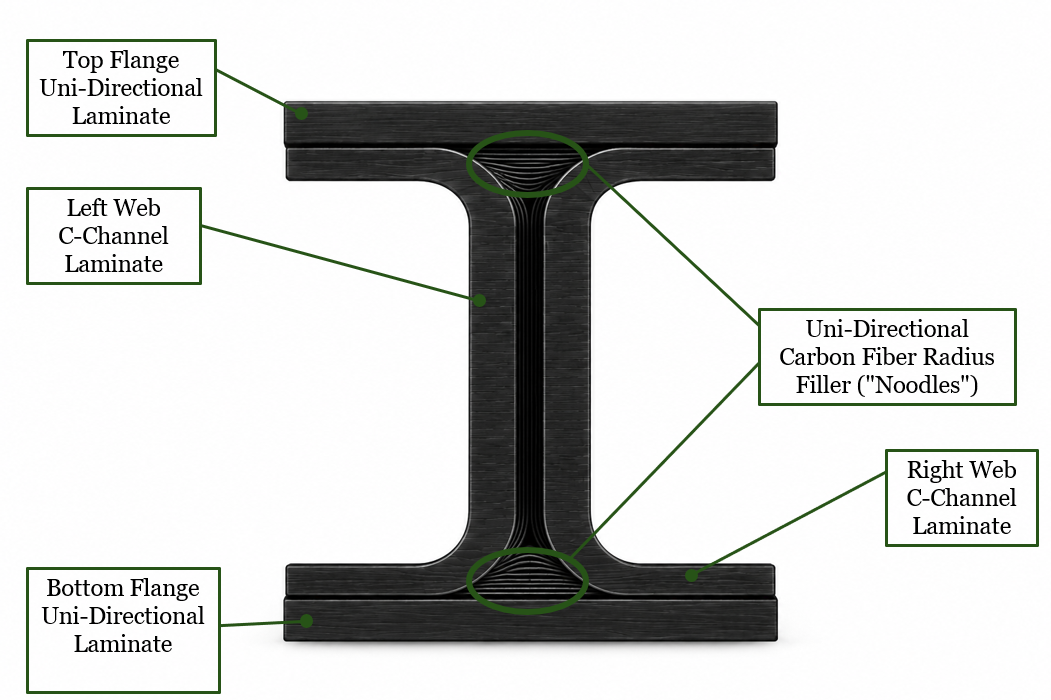
\includegraphics[
        width=3.55in,
        height=2.45in,
        keepaspectratio
    ]{front view assembly graphic.png}
};

\node[
    anchor=north,
    align=center,
    inner sep=0pt,
    text width=3.42in,
    text=Muted,
    font=\sffamily\fontsize{6.35}{7.05}\selectfont
]
at ($(current page.north west)+(2.195in,-4.12in)$)
{Four-piece laminate architecture with top and bottom flange laminates, paired C-channels, and longitudinal radius fillers};

% ============================================================
% TOP CENTER — PROJECT OVERVIEW + C-CHANNEL LAYUP
% ============================================================

\fill[SoftGold,rounded corners=5pt]
    ($(current page.north west)+(4.18in,-1.58in)$)
    rectangle
    ($(current page.north west)+(7.42in,-4.20in)$);

\fill[PolyGold]
    ($(current page.north west)+(4.18in,-1.58in)$)
    rectangle
    ($(current page.north west)+(4.28in,-4.20in)$);

\node[
    anchor=north west,
    text=DeepGreen,
    font=\sffamily\bfseries\fontsize{8.0}{8.7}\selectfont
]
at ($(current page.north west)+(4.48in,-1.76in)$)
{PROJECT OVERVIEW};

\node[
    anchor=north west,
    align=left,
    text width=2.64in,
    text=Ink,
    font=\fontsize{6.40}{7.45}\selectfont
]
at ($(current page.north west)+(4.48in,-2.04in)$)
{
A 24-inch carbon-fiber I-beam was manufactured from two molded
C-channel laminates, separate top and bottom flange laminates,
and longitudinal unidirectional radius fillers. The completed
684 g specimen sustained 28.2 kN (6,340 lbf) in three-point bending.\\[3pt]
\textbf{C-channel layup.}
Each channel used the same 12-ply sequence:
\mbox{$[+45/-45/0/+45/-45/0/0/-45/+45/0/-45/+45]$}.
The layup was completed twice, once for each channel.\\[3pt]
\textbf{Flange layups.}
Top flange: \mbox{$[90/0_6/90/0_6]$}. Bottom flange:
\mbox{$[90/0_6]$}, where $0_6$ denotes six consecutive 0-degree plies.
};

\node[
    anchor=south west,
    text=PolyGold,
    font=\sffamily\bfseries\fontsize{6.45}{7.1}\selectfont
]
at ($(current page.north west)+(4.48in,-4.03in)$)
{MASS: 684 g \hspace{8pt}\textbullet\hspace{8pt} PEAK LOAD: 28.2 kN \hspace{8pt}\textbullet\hspace{8pt} LENGTH: 24 in};

% ============================================================
% TOP RIGHT — C-CHANNEL MANUFACTURING
% ============================================================

\node[
    anchor=north west,
    inner sep=2.6pt,
    draw=DeepGreen,
    line width=0.68pt,
    rounded corners=5pt
]
at ($(current page.north west)+(7.62in,-1.58in)$)
{
    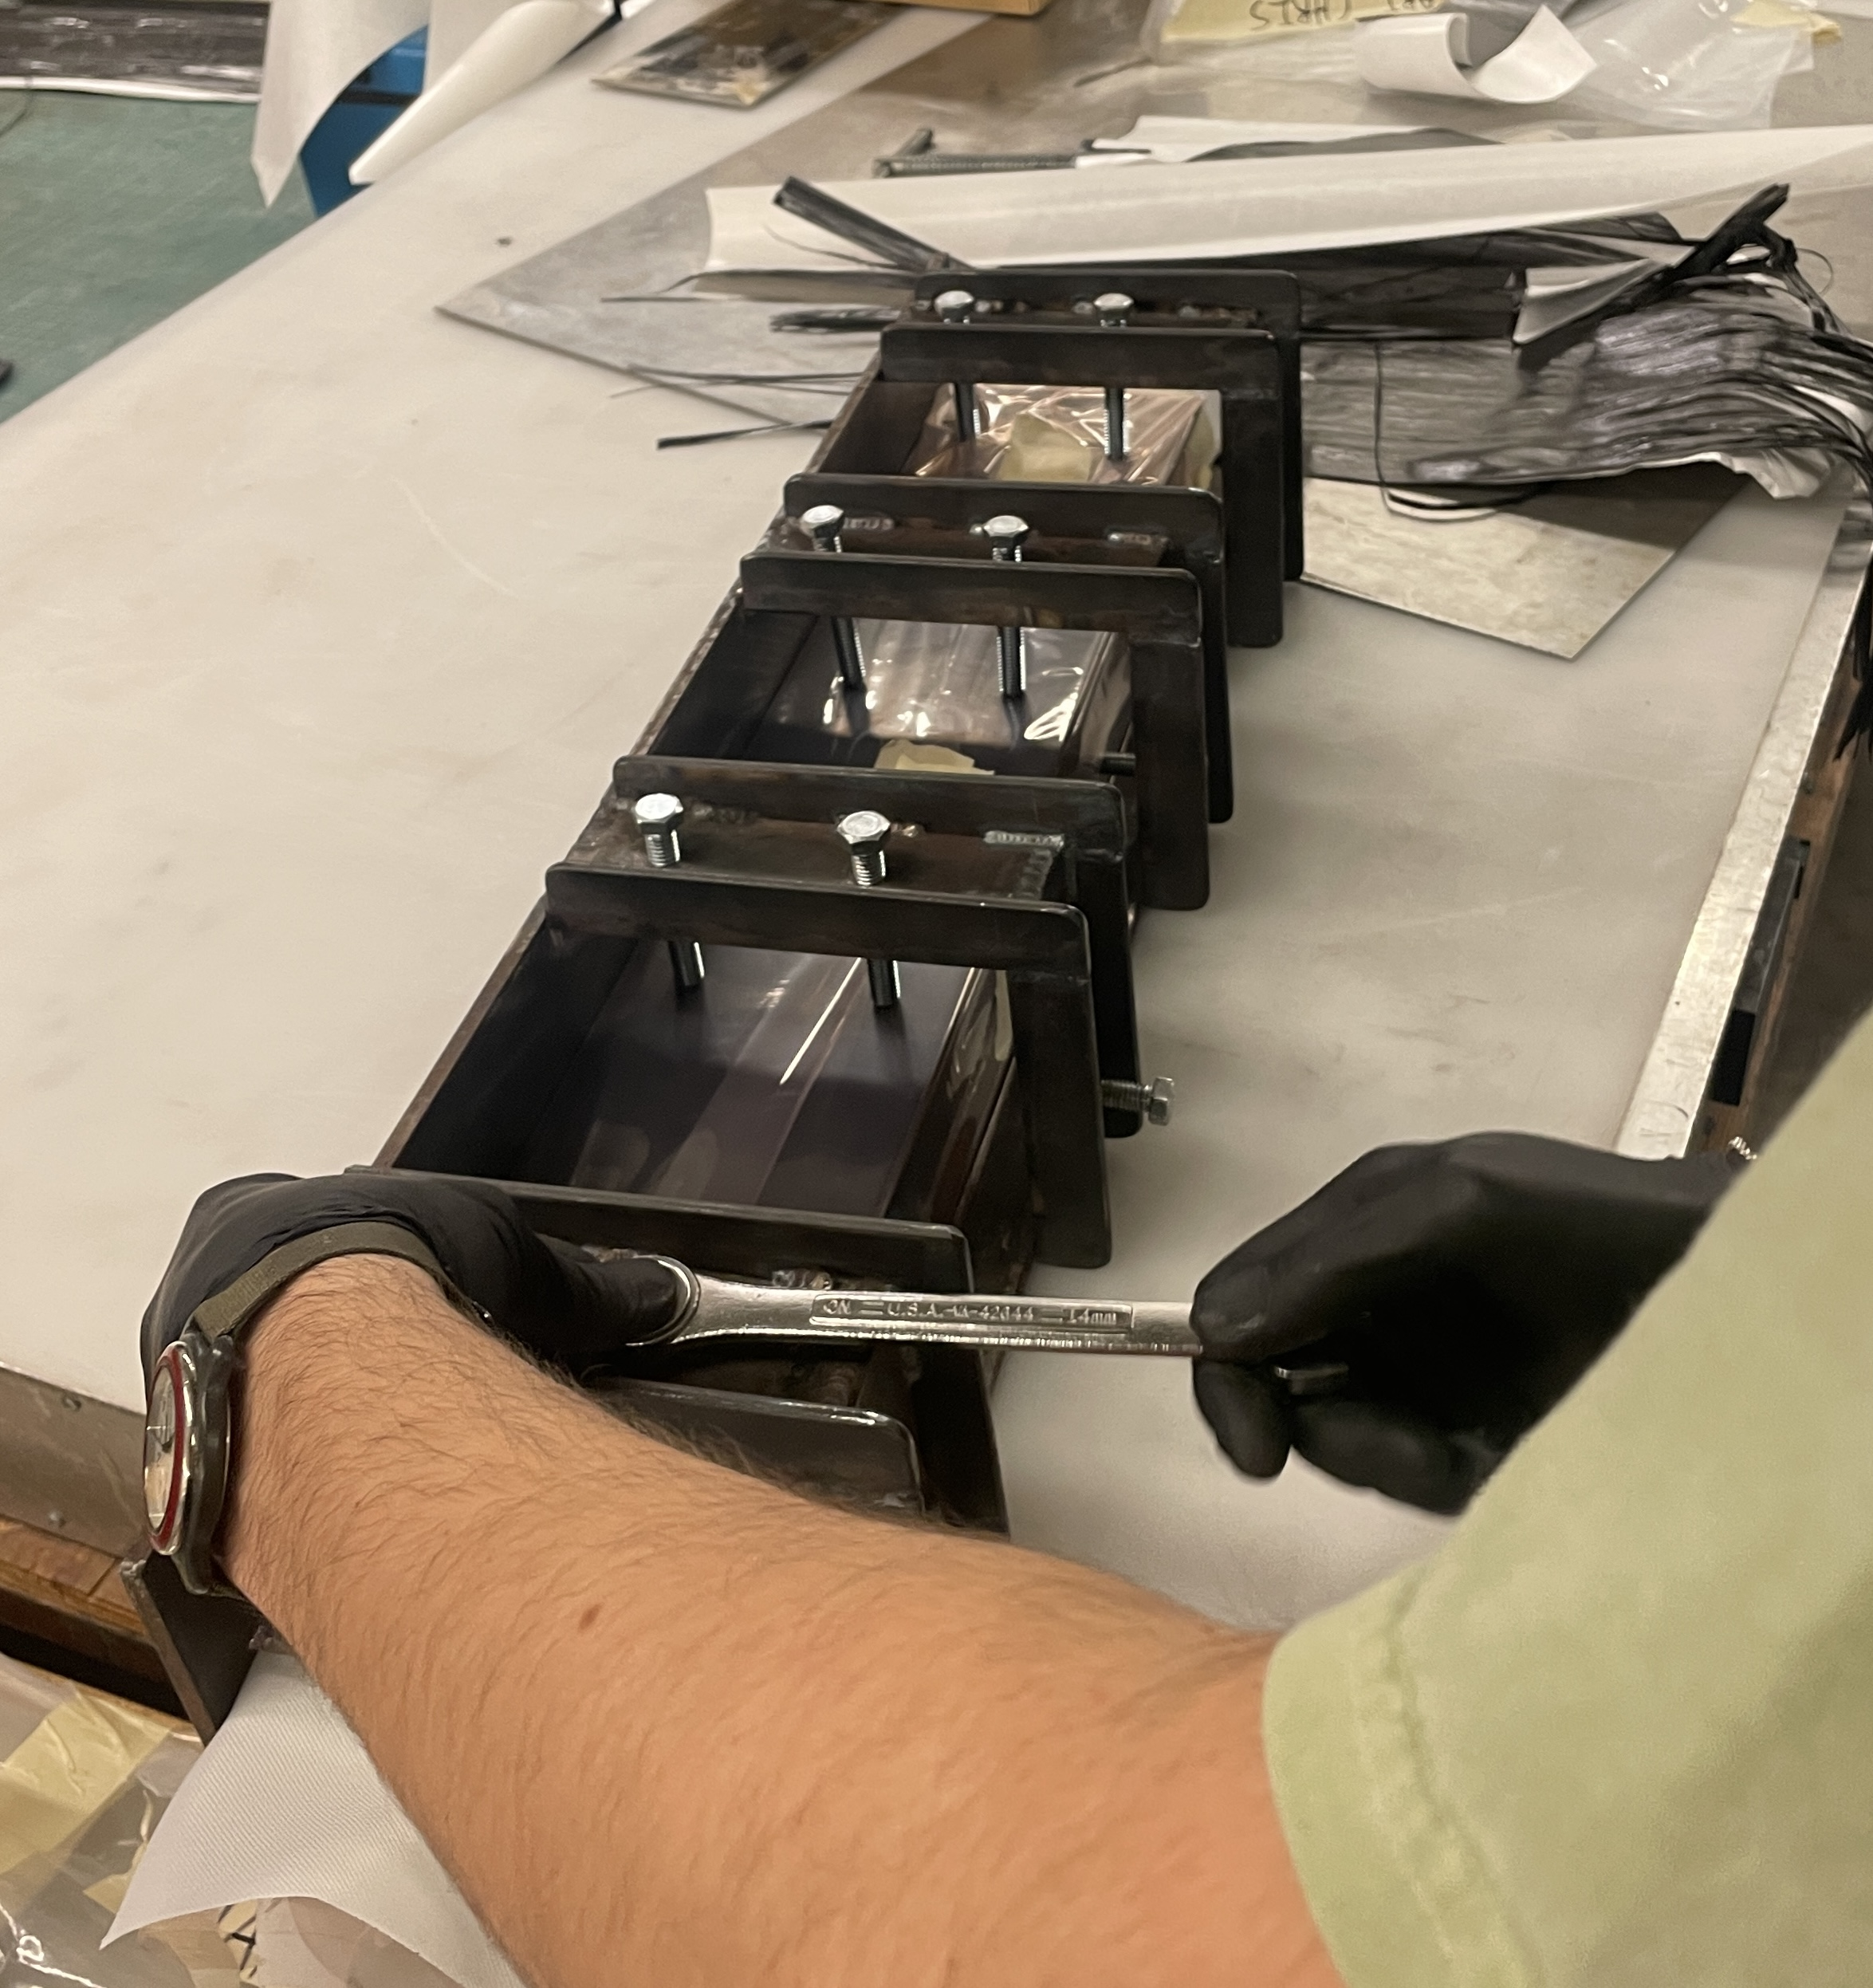
\includegraphics[
        width=3.55in,
        height=2.45in,
        keepaspectratio
    ]{Distributed weight with bolts.jpg}
};

\node[
    anchor=north,
    align=center,
    inner sep=0pt,
    text width=3.42in,
    text=Muted,
    font=\sffamily\fontsize{6.35}{7.05}\selectfont
]
at ($(current page.north west)+(9.395in,-4.12in)$)
{Distributed bolt pressure maintained alignment and consolidated the full beam assembly during cure};

% ============================================================
% CENTER ROW — MODEL, TEST, AND OBSERVED FAILURE
% ============================================================

\node[
    anchor=north west,
    inner sep=2.4pt,
    draw=RuleGray,
    line width=0.55pt,
    rounded corners=4pt
]
at ($(current page.north west)+(0.42in,-4.43in)$)
{
    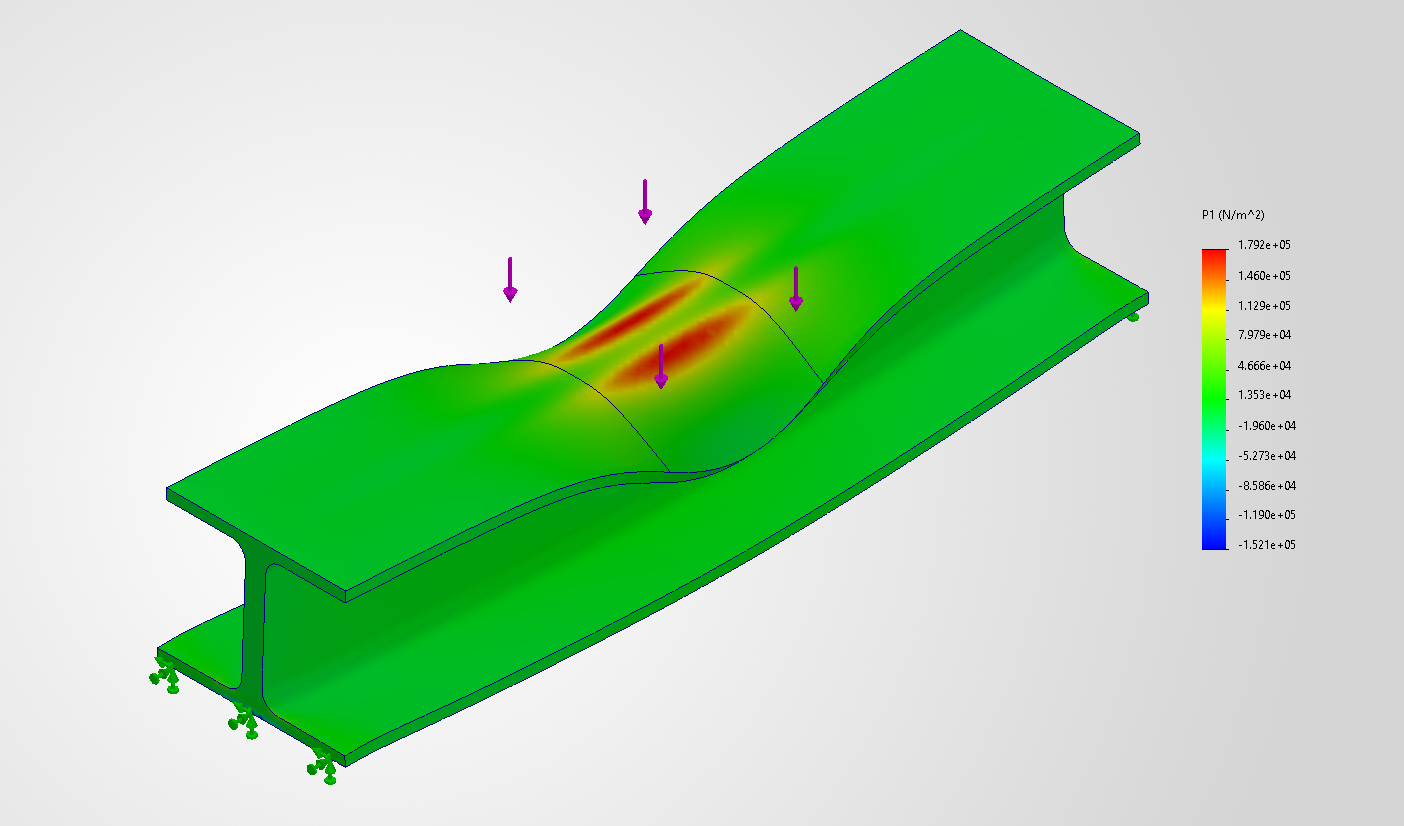
\includegraphics[
        width=3.33in,
        height=1.62in,
        keepaspectratio
    ]{Stress Analysis on Generic CAD model.png}
};

\node[
    anchor=north,
    align=center,
    inner sep=0pt,
    text width=3.20in,
    text=Muted,
    font=\sffamily\fontsize{6.20}{6.85}\selectfont
]
at ($(current page.north west)+(2.085in,-6.14in)$)
{Generic FEA predicted peak compressive stress beneath the center loading shoe};

\node[
    anchor=north west,
    inner sep=2.4pt,
    draw=RuleGray,
    line width=0.55pt,
    rounded corners=4pt
]
at ($(current page.north west)+(3.92in,-4.43in)$)
{
    \includegraphics[
        angle=180,
        origin=c,
        width=3.18in,
        height=1.62in,
        keepaspectratio
    ]{Three Point Bend Test.JPG}
};

\node[
    anchor=north,
    align=center,
    inner sep=0pt,
    text width=3.05in,
    text=Muted,
    font=\sffamily\fontsize{6.20}{6.85}\selectfont
]
at ($(current page.north west)+(5.510in,-6.14in)$)
{Experimental three-point bend test on the completed I-beam specimen};

\node[
    anchor=north west,
    inner sep=2.4pt,
    draw=RuleGray,
    line width=0.55pt,
    rounded corners=4pt
]
at ($(current page.north west)+(7.28in,-4.43in)$)
{
    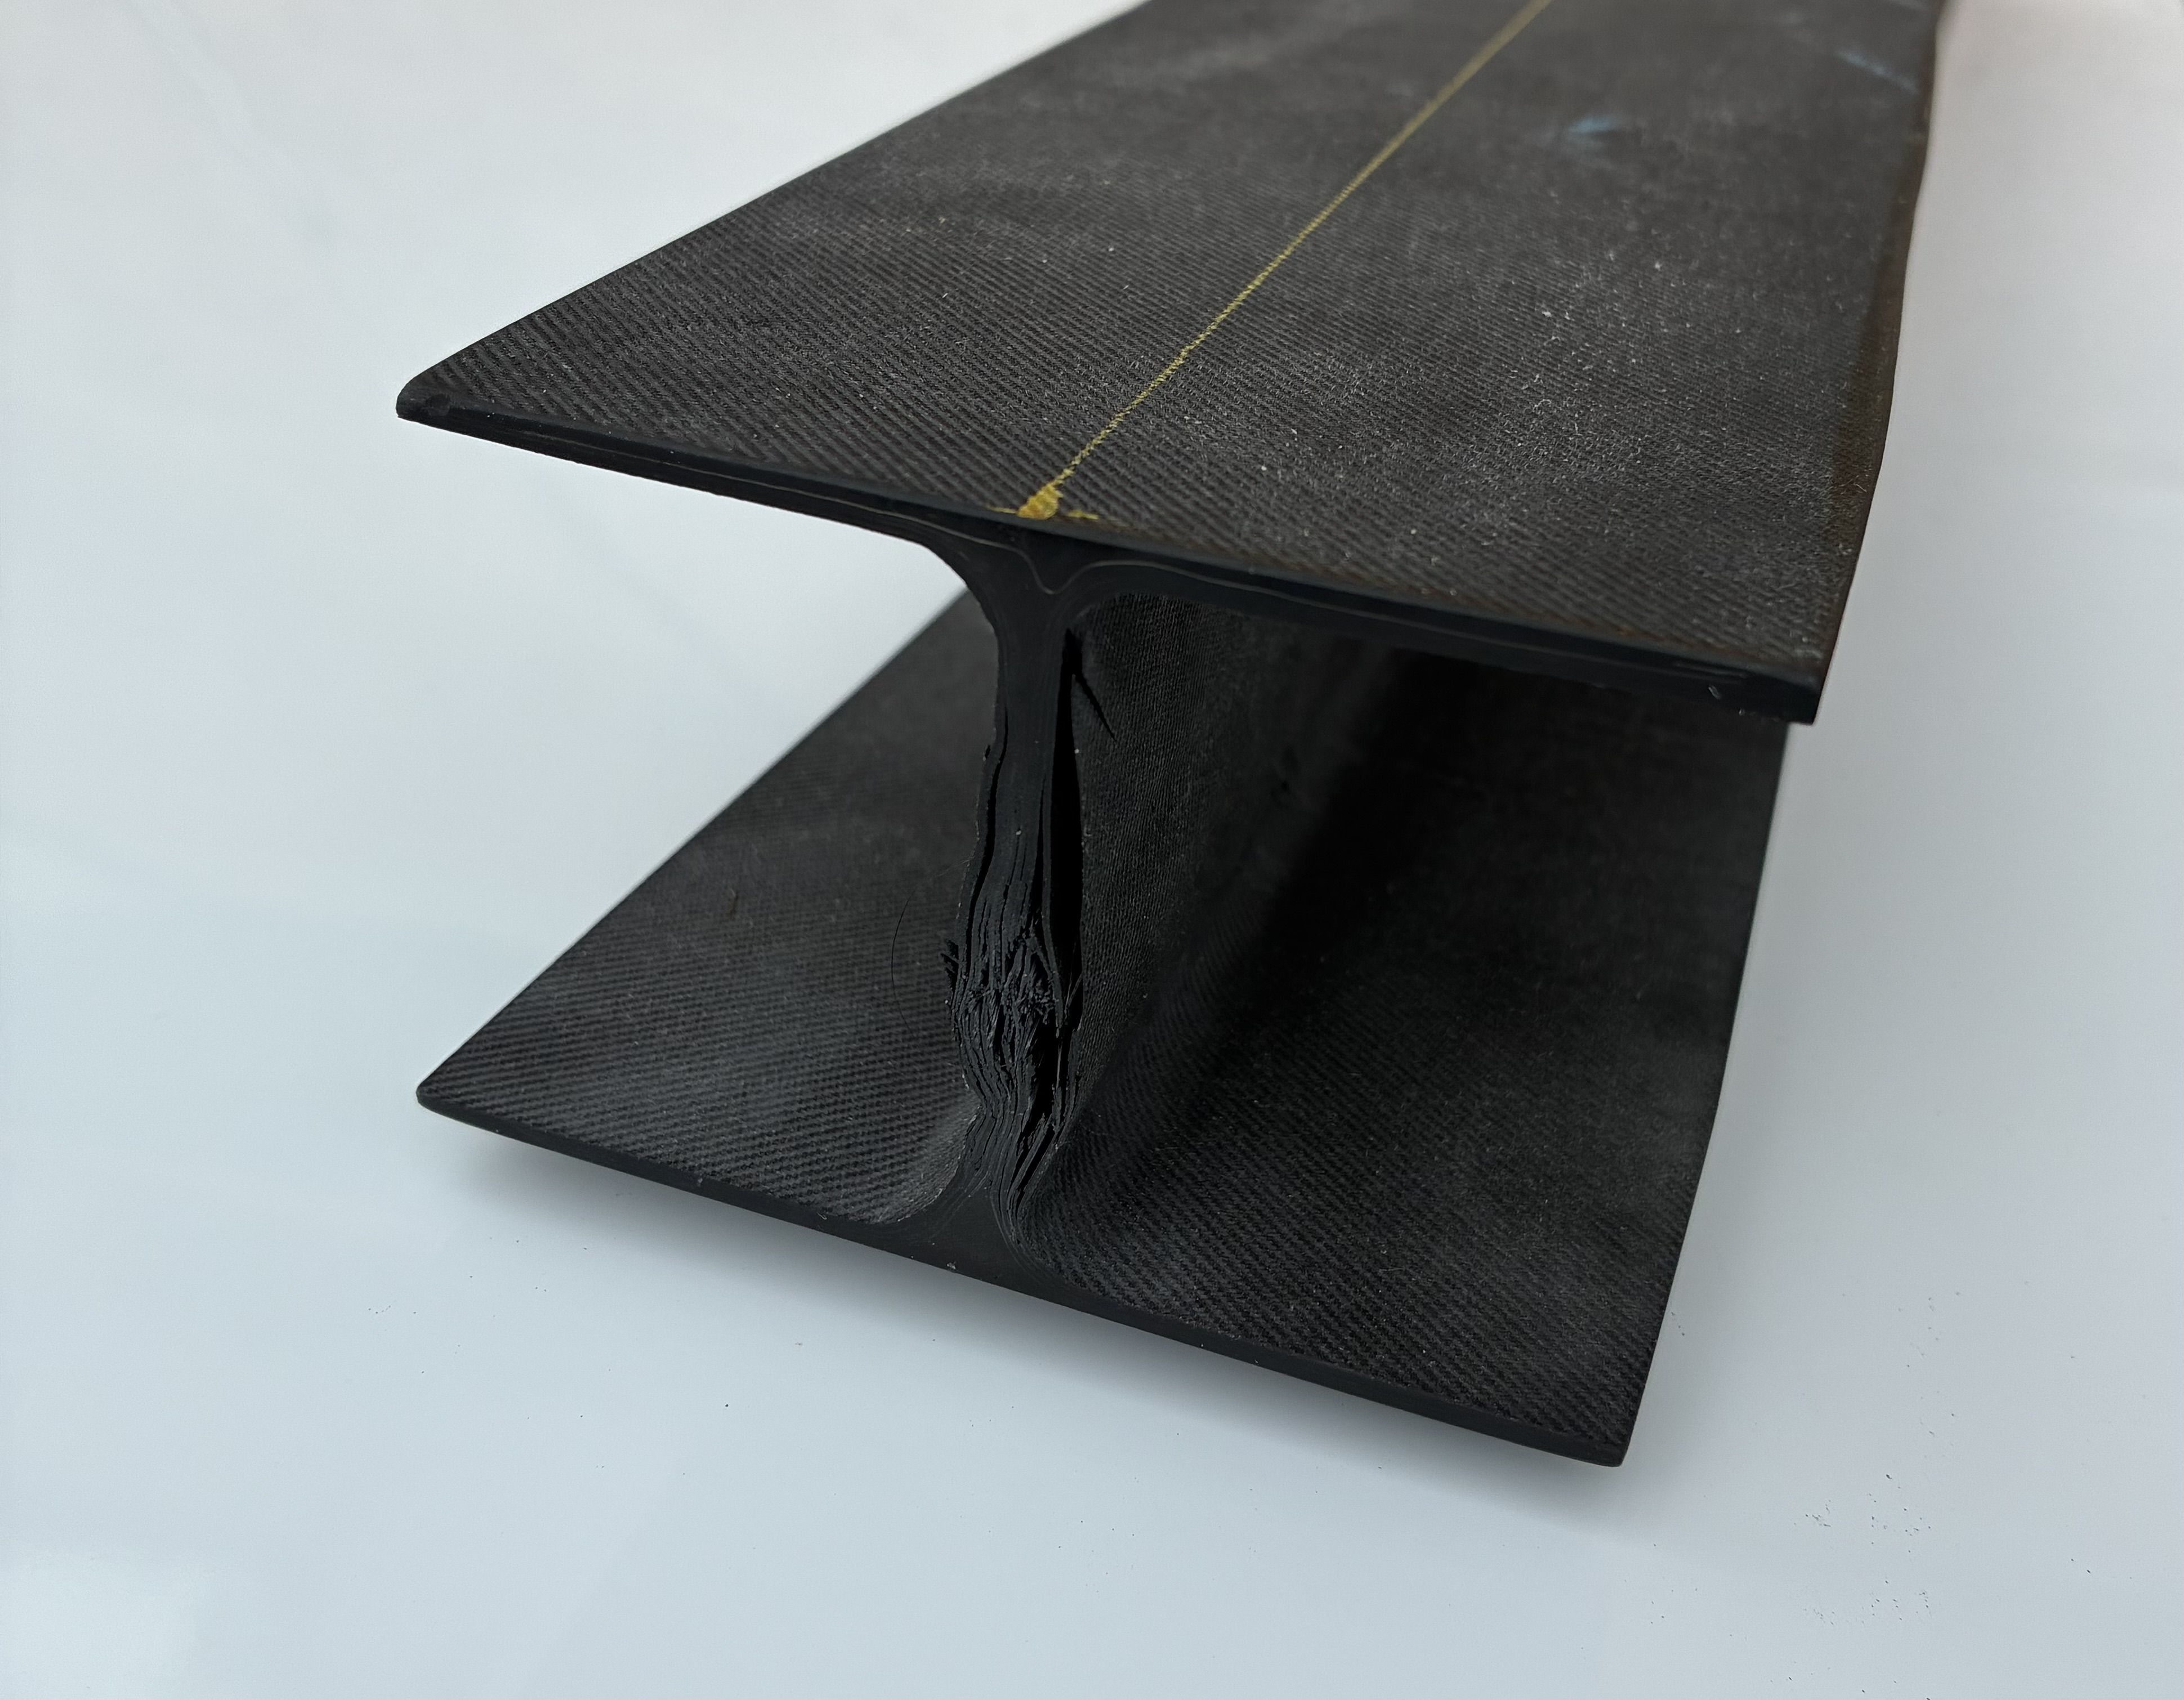
\includegraphics[
        width=3.65in,
        height=1.62in,
        keepaspectratio
    ]{Beam Fiulure Delamination and cracking.jpeg}
};

\node[
    anchor=north,
    align=center,
    inner sep=0pt,
    text width=3.50in,
    text=Muted,
    font=\sffamily\fontsize{6.20}{6.85}\selectfont
]
at ($(current page.north west)+(9.105in,-6.14in)$)
{Observed edge failure with delamination and longitudinal crack propagation};

% ============================================================
% BOTTOM LEFT — MANUFACTURING PROCESS
% ============================================================

\fill[SoftGreen,rounded corners=5pt]
    ($(current page.north west)+(0.42in,-6.43in)$)
    rectangle
    ($(current page.north west)+(5.30in,-7.18in)$);

\draw[RuleGray,line width=0.55pt,rounded corners=5pt]
    ($(current page.north west)+(0.42in,-6.43in)$)
    rectangle
    ($(current page.north west)+(5.30in,-7.18in)$);

\node[
    anchor=north west,
    text=DeepGreen,
    font=\sffamily\bfseries\fontsize{7.65}{8.35}\selectfont
]
at ($(current page.north west)+(0.66in,-6.57in)$)
{MANUFACTURING APPROACH};

\node[
    anchor=north west,
    align=left,
    text width=4.38in,
    text=Ink,
    font=\fontsize{6.20}{7.15}\selectfont
]
at ($(current page.north west)+(0.66in,-6.82in)$)
{
The separately molded channels were aligned with longitudinal carbon-fiber
``noodles'' filling the radius-induced flange voids. Top and bottom flanges
were then installed, and the full assembly was consolidated in a custom
steel fixture using distributed bolt pressure along the beam length.
};

% ============================================================
% BOTTOM RIGHT — FAILURE ANALYSIS AND NEXT ITERATION
% ============================================================

\fill[SoftGold,rounded corners=5pt]
    ($(current page.north west)+(5.52in,-6.43in)$)
    rectangle
    ($(current page.north east)+(-0.42in,-7.18in)$);

\fill[PolyGold]
    ($(current page.north west)+(5.52in,-6.43in)$)
    rectangle
    ($(current page.north west)+(5.62in,-7.18in)$);

\node[
    anchor=north west,
    text=DeepGreen,
    font=\sffamily\bfseries\fontsize{7.65}{8.35}\selectfont
]
at ($(current page.north west)+(5.82in,-6.57in)$)
{FAILURE ANALYSIS AND NEXT ITERATION};

\node[
    anchor=north west,
    align=left,
    text width=4.72in,
    text=Ink,
    font=\fontsize{6.14}{7.08}\selectfont
]
at ($(current page.north west)+(5.82in,-6.82in)$)
{
The model suggested a center-span compression failure, but the physical beam
failed near its edge. This mismatch indicates that local consolidation defects
likely enabled premature delamination. A future build should use staged vacuum
debulking after each ply group rather than relying only on manual rolling before
final fixture consolidation.
};

% ============================================================
% RESOURCE LINKS
% ============================================================

\node[
    anchor=north,
    align=center,
    text=DeepGreen,
    font=\sffamily\bfseries\fontsize{6.75}{7.35}\selectfont
]
at ($(current page.north)+(0,-7.43in)$)
{
\href{\IBeamCompetitionGuidelines}{\faFilePdf\ COMPETITION GUIDELINES}
\hspace{16pt}
\href{\IBeamBendTestVideo}{\faPlayCircle\ THREE-POINT BEND TEST VIDEO}
};

% ============================================================
% FOOTER
% ============================================================

\node[
    anchor=south west,
    text=white,
    font=\sffamily\bfseries\fontsize{7.1}{7.7}\selectfont
]
at ($(current page.south west)+(0.42in,0.17in)$)
{\hyperlink{pickleball}{\faArrowLeft\ PICKLEBALL PADDLE}};

\node[
    anchor=south,
    text=white,
    font=\sffamily\fontsize{7.0}{7.6}\selectfont
]
at ($(current page.south)+(0,0.17in)$)
{CARBON FIBER I-BEAM \hspace{6pt} 1 / 1};

\node[
    anchor=south east,
    text=white,
    font=\sffamily\bfseries\fontsize{7.1}{7.7}\selectfont
]
at ($(current page.south east)+(-0.42in,0.17in)$)
{NEXT PROJECT \faArrowRight};

\end{tikzpicture}
% ============================================================
% FIBERGLASS FUSELAGE FEA & THREE-POINT BEND VALIDATION
% SINGLE-PAGE PORTFOLIO CASE STUDY
% 01 Composites / Project 04
%
% IMPORTANT:
% 1. This file must NOT contain \documentclass, \begin{document},
%    or \end{document}.
% 2. In main.tex, place % ============================================================
% FIBERGLASS FUSELAGE FEA & THREE-POINT BEND VALIDATION
% SINGLE-PAGE PORTFOLIO CASE STUDY
% 01 Composites / Project 04
%
% IMPORTANT:
% 1. This file must NOT contain \documentclass, \begin{document},
%    or \end{document}.
% 2. In main.tex, place \input{fuselage} before \end{document}.
% 3. This script assumes the main portfolio preamble already defines:
%       DeepGreen, PolyGold, SoftGold, SoftGreen,
%       RuleGray, Muted, Ink
%    and loads tikz, graphicx, hyperref, and fontawesome5.
% 4. Upload these files to Overleaf with the exact same names:
%       Setup & Mesh of FEA.png
%       fuselage 3 point bend test.JPG
%       Countor Plot of Reaction Force.png
%       fuselage data.png
% ============================================================

\providecommand{\FuselageDemoVideo}
{https://drive.google.com/file/d/1xFCbBJXPhVVlnaleRyZeSM8ucD_xWwB2/view?usp=drive_link}

\providecommand{\FuselageFinalReport}
{https://drive.google.com/file/d/1LYRNlwk73l_KRgaSPgzfsYis-9bsuaxX/view?usp=drive_link}

\clearpage
\thispagestyle{empty}
\hypertarget{fuselage}{}
\null

\begin{tikzpicture}[remember picture,overlay]

% ============================================================
% BACKGROUND AND PAGE BARS
% ============================================================

\fill[white]
    (current page.south west)
    rectangle
    (current page.north east);

\fill[DeepGreen]
    (current page.north west)
    rectangle
    ($(current page.north east)+(0,-0.095in)$);

\fill[PolyGold]
    ($(current page.north west)+(0,-0.095in)$)
    rectangle
    ($(current page.north east)+(0,-0.14in)$);

\fill[DeepGreen]
    (current page.south west)
    rectangle
    ($(current page.south east)+(0,0.36in)$);

\fill[PolyGold]
    ($(current page.south west)+(0,0.36in)$)
    rectangle
    ($(current page.south east)+(0,0.405in)$);

% ============================================================
% HEADER
% ============================================================

\node[
    anchor=north west,
    text=PolyGold,
    font=\sffamily\bfseries\fontsize{8.1}{8.7}\selectfont
]
at ($(current page.north west)+(0.42in,-0.39in)$)
{01 COMPOSITES \hspace{5pt}/\hspace{5pt} PROJECT 04};

\node[
    anchor=north west,
    text=DeepGreen,
    font=\bfseries\fontsize{20.8}{21.8}\selectfont
]
at ($(current page.north west)+(0.40in,-0.67in)$)
{FIBERGLASS FUSELAGE FEA \& THREE-POINT BEND VALIDATION};

\node[
    anchor=north west,
    text=Muted,
    font=\sffamily\fontsize{8.15}{8.9}\selectfont
]
at ($(current page.north west)+(0.42in,-1.12in)$)
{Cal Poly Composites Laboratory \hspace{7pt}\textbullet\hspace{7pt}
Individual Project \hspace{7pt}\textbullet\hspace{7pt}
Winter 2026 \hspace{7pt}\textbullet\hspace{7pt}
San Luis Obispo, California};

\fill[PolyGold]
    ($(current page.north west)+(0.42in,-1.36in)$)
    rectangle
    ($(current page.north west)+(6.10in,-1.315in)$);


% ============================================================
% TOP LEFT — ABAQUS MODEL SETUP
% ============================================================

\node[
    anchor=north west,
    inner sep=2.6pt,
    draw=DeepGreen,
    line width=0.68pt,
    rounded corners=5pt
]
at ($(current page.north west)+(0.42in,-1.58in)$)
{
    \includegraphics[
        width=3.55in,
        height=2.34in,
        keepaspectratio
    ]{\detokenize{Setup & Mesh of FEA.png}}
};

\node[
    anchor=north,
    align=center,
    inner sep=0pt,
    text width=3.42in,
    text=Muted,
    font=\sffamily\fontsize{6.30}{7.00}\selectfont
]
at ($(current page.north west)+(2.195in,-4.02in)$)
{Abaqus assembly and quad-dominated mesh for the composite shell fuselage and rigid loading fixtures};

% ============================================================
% TOP CENTER — PROJECT OVERVIEW / STAR SUMMARY
% ============================================================

\fill[SoftGold,rounded corners=5pt]
    ($(current page.north west)+(4.18in,-1.58in)$)
    rectangle
    ($(current page.north west)+(8.55in,-4.10in)$);

\fill[PolyGold]
    ($(current page.north west)+(4.18in,-1.58in)$)
    rectangle
    ($(current page.north west)+(4.28in,-4.10in)$);

\node[
    anchor=north west,
    text=DeepGreen,
    font=\sffamily\bfseries\fontsize{8.0}{8.7}\selectfont
]
at ($(current page.north west)+(4.48in,-1.76in)$)
{PROJECT OVERVIEW};

\node[
    anchor=north west,
    align=left,
    text width=3.38in,
    text=Ink,
    font=\fontsize{6.28}{7.28}\selectfont
]
at ($(current page.north west)+(4.48in,-2.03in)$)
{
I developed and validated a seven-ply fiberglass fuselage model under a SAMPE-inspired three-point bend configuration. The Abaqus model reproduced the physical geometry, composite layup, rigid tooling, contact interactions, and displacement-controlled loading used during testing. I defined equivalent orthotropic lamina properties, preserved the 4-inch inner diameter through shell offset, created rigid-body reference points, and evaluated transverse-shear assumptions through sensitivity studies. The model correctly identified the experimentally observed critical region beneath the loading shoe, while the simulation-to-test comparison revealed the limitations of idealized composite failure modeling and guided a more defensible interpretation of the results.
};

\node[
    anchor=south west,
    text=PolyGold,
    font=\sffamily\bfseries\fontsize{6.35}{7.0}\selectfont
]
at ($(current page.north west)+(4.48in,-3.94in)$)
{7 PLIES \hspace{7pt}\textbullet\hspace{7pt} 20,584 SHELL ELEMENTS \hspace{7pt}\textbullet\hspace{7pt} 2 in DISPLACEMENT};

% ============================================================
% TOP RIGHT — PHYSICAL TEST
% ============================================================

\node[
    anchor=north west,
    inner sep=2.6pt,
    draw=DeepGreen,
    line width=0.68pt,
    rounded corners=5pt
]
at ($(current page.north west)+(8.70in,-1.58in)$)
{
    \includegraphics[
        angle=-90,
        origin=c,
        width=3.18in,
        height=2.18in,
        keepaspectratio
    ]{\detokenize{fuselage 3 point bend test.JPG}}
};

\node[
    anchor=north,
    align=center,
    inner sep=0pt,
    text width=2.70in,
    text=Muted,
    font=\sffamily\fontsize{6.30}{7.00}\selectfont
]
at ($(current page.north west)+(9.95in,-4.21in)$)
{Three-point bend validation test};

% ============================================================
% CENTER ROW — SIMULATION RESPONSE AND EXPERIMENTAL DATA
% ============================================================

% Left response card
\fill[SoftGreen!42,rounded corners=5pt]
    ($(current page.north west)+(0.42in,-4.34in)$)
    rectangle
    ($(current page.north west)+(6.60in,-6.28in)$);

\draw[RuleGray,line width=0.55pt,rounded corners=5pt]
    ($(current page.north west)+(0.42in,-4.34in)$)
    rectangle
    ($(current page.north west)+(5.55in,-6.28in)$);

\node[
    anchor=north west,
    text=DeepGreen,
    font=\sffamily\bfseries\fontsize{7.10}{7.75}\selectfont
]
at ($(current page.north west)+(0.66in,-4.48in)$)
{ABAQUS RESPONSE};

\node[
    anchor=north,
    inner sep=0pt
]
at ($(current page.north west)+(2.985in,-4.70in)$)
{
    \includegraphics[
        width=4.70in,
        height=1.26in,
        keepaspectratio
    ]{\detokenize{Countor Plot of Reaction Force.png}}
};

\node[
    anchor=north,
    align=center,
    inner sep=0pt,
    text width=4.55in,
    text=Muted,
    font=\sffamily\fontsize{6.15}{6.85}\selectfont
]
at ($(current page.north west)+(2.985in,-6.08in)$)
{Abaqus reaction-force response under bending};

% Right response card
\fill[SoftGreen!42,rounded corners=5pt]
    ($(current page.north west)+(5.76in,-4.34in)$)
    rectangle
    ($(current page.north east)+(-0.42in,-6.28in)$);

\draw[RuleGray,line width=0.55pt,rounded corners=5pt]
    ($(current page.north west)+(5.76in,-4.34in)$)
    rectangle
    ($(current page.north east)+(-0.42in,-6.28in)$);

\node[
    anchor=north west,
    text=DeepGreen,
    font=\sffamily\bfseries\fontsize{7.10}{7.75}\selectfont
]
at ($(current page.north west)+(6.00in,-4.48in)$)
{EXPERIMENTAL RESPONSE};

\node[
    anchor=north,
    inner sep=0pt
]
at ($(current page.north west)+(8.425in,-4.68in)$)
{
    \includegraphics[
        width=4.58in,
        height=1.32in,
        keepaspectratio
    ]{\detokenize{fuselage data.png}}
};

\node[
    anchor=north,
    align=center,
    inner sep=0pt,
    text width=4.45in,
    text=Muted,
    font=\sffamily\fontsize{6.15}{6.85}\selectfont
]
at ($(current page.north west)+(8.425in,-6.08in)$)
{Measured load history and peak response};

% ============================================================
% BOTTOM LEFT — MODELING APPROACH
% ============================================================

\fill[SoftGreen,rounded corners=5pt]
    ($(current page.north west)+(0.42in,-6.50in)$)
    rectangle
    ($(current page.north west)+(5.34in,-7.45in)$);

\draw[RuleGray,line width=0.55pt,rounded corners=5pt]
    ($(current page.north west)+(0.42in,-6.50in)$)
    rectangle
    ($(current page.north west)+(5.34in,-7.45in)$);

\node[
    anchor=north west,
    text=DeepGreen,
    font=\sffamily\bfseries\fontsize{7.65}{8.35}\selectfont
]
at ($(current page.north west)+(0.66in,-6.64in)$)
{MODELING APPROACH};

\node[
    anchor=north west,
    align=left,
    text width=4.44in,
    text=Ink,
    font=\fontsize{6.08}{7.02}\selectfont
]
at ($(current page.north west)+(0.66in,-6.89in)$)
{
The fuselage was represented as a seven-ply woven-fiberglass composite shell.
Rigid upper and lower fixtures transferred load through frictional contact, while
two static steps imposed 2 inches of total downward displacement. High- and
low-case studies for $G_{13}$ and $G_{23}$ changed peak reaction force by only
about 1.8\%, showing that the global response was not dominated by those assumptions.
};

% ============================================================
% BOTTOM RIGHT — VALIDATION AND ENGINEERING JUDGMENT
% ============================================================

\fill[SoftGold,rounded corners=5pt]
    ($(current page.north west)+(5.56in,-6.50in)$)
    rectangle
    ($(current page.north east)+(-0.42in,-7.45in)$);

\fill[PolyGold]
    ($(current page.north west)+(5.56in,-6.50in)$)
    rectangle
    ($(current page.north west)+(5.66in,-7.45in)$);

\node[
    anchor=north west,
    text=DeepGreen,
    font=\sffamily\bfseries\fontsize{7.65}{8.35}\selectfont
]
at ($(current page.north west)+(5.86in,-6.64in)$)
{VALIDATION AND ENGINEERING JUDGMENT};

\node[
    anchor=north west,
    align=left,
    text width=4.66in,
    text=Ink,
    font=\fontsize{6.02}{6.96}\selectfont
]
at ($(current page.north west)+(5.86in,-6.89in)$)
{
Abaqus predicted 1,814 lbf versus the measured 1,123.82 lbf, an overprediction
of 61.4\%. Rather than treating the model as fully validated, I traced the gap to
approximated material properties, idealized shell geometry, simplified contact,
and the absence of progressive crushing, delamination, and tear-through.
The study demonstrated both technical persistence and the judgment to distinguish
useful qualitative agreement from unsupported quantitative confidence.
};

% ============================================================
% RESOURCE LINKS
% ============================================================

\node[
    anchor=north,
    align=center,
    text=DeepGreen,
    font=\sffamily\bfseries\fontsize{6.75}{7.35}\selectfont
]
at ($(current page.north)+(0,-7.56in)$)
{
\href{\FuselageFinalReport}{\faFilePdf\ FINAL ANALYSIS REPORT}
\hspace{16pt}
\href{\FuselageDemoVideo}{\faPlayCircle\ FUSELAGE DEMONSTRATION}
};

% ============================================================
% FOOTER
% ============================================================

\node[
    anchor=south west,
    text=white,
    font=\sffamily\bfseries\fontsize{7.1}{7.7}\selectfont
]
at ($(current page.south west)+(0.42in,0.17in)$)
{\hyperlink{ibeam}{\faArrowLeft\ CARBON FIBER I-BEAM}};

\node[
    anchor=south,
    text=white,
    font=\sffamily\fontsize{7.0}{7.6}\selectfont
]
at ($(current page.south)+(0,0.17in)$)
{FIBERGLASS FUSELAGE \hspace{6pt} 1 / 1};

\node[
    anchor=south east,
    text=white,
    font=\sffamily\bfseries\fontsize{7.1}{7.7}\selectfont
]
at ($(current page.south east)+(-0.42in,0.17in)$)
{NEXT PROJECT \faArrowRight};

\end{tikzpicture}
\input{coupons}
\clearpage
 before \end{document}.
% 3. This script assumes the main portfolio preamble already defines:
%       DeepGreen, PolyGold, SoftGold, SoftGreen,
%       RuleGray, Muted, Ink
%    and loads tikz, graphicx, hyperref, and fontawesome5.
% 4. Upload these files to Overleaf with the exact same names:
%       Setup & Mesh of FEA.png
%       fuselage 3 point bend test.JPG
%       Countor Plot of Reaction Force.png
%       fuselage data.png
% ============================================================

\providecommand{\FuselageDemoVideo}
{https://drive.google.com/file/d/1xFCbBJXPhVVlnaleRyZeSM8ucD_xWwB2/view?usp=drive_link}

\providecommand{\FuselageFinalReport}
{https://drive.google.com/file/d/1LYRNlwk73l_KRgaSPgzfsYis-9bsuaxX/view?usp=drive_link}

\clearpage
\thispagestyle{empty}
\hypertarget{fuselage}{}
\null

\begin{tikzpicture}[remember picture,overlay]

% ============================================================
% BACKGROUND AND PAGE BARS
% ============================================================

\fill[white]
    (current page.south west)
    rectangle
    (current page.north east);

\fill[DeepGreen]
    (current page.north west)
    rectangle
    ($(current page.north east)+(0,-0.095in)$);

\fill[PolyGold]
    ($(current page.north west)+(0,-0.095in)$)
    rectangle
    ($(current page.north east)+(0,-0.14in)$);

\fill[DeepGreen]
    (current page.south west)
    rectangle
    ($(current page.south east)+(0,0.36in)$);

\fill[PolyGold]
    ($(current page.south west)+(0,0.36in)$)
    rectangle
    ($(current page.south east)+(0,0.405in)$);

% ============================================================
% HEADER
% ============================================================

\node[
    anchor=north west,
    text=PolyGold,
    font=\sffamily\bfseries\fontsize{8.1}{8.7}\selectfont
]
at ($(current page.north west)+(0.42in,-0.39in)$)
{01 COMPOSITES \hspace{5pt}/\hspace{5pt} PROJECT 04};

\node[
    anchor=north west,
    text=DeepGreen,
    font=\bfseries\fontsize{20.8}{21.8}\selectfont
]
at ($(current page.north west)+(0.40in,-0.67in)$)
{FIBERGLASS FUSELAGE FEA \& THREE-POINT BEND VALIDATION};

\node[
    anchor=north west,
    text=Muted,
    font=\sffamily\fontsize{8.15}{8.9}\selectfont
]
at ($(current page.north west)+(0.42in,-1.12in)$)
{Cal Poly Composites Laboratory \hspace{7pt}\textbullet\hspace{7pt}
Individual Project \hspace{7pt}\textbullet\hspace{7pt}
Winter 2026 \hspace{7pt}\textbullet\hspace{7pt}
San Luis Obispo, California};

\fill[PolyGold]
    ($(current page.north west)+(0.42in,-1.36in)$)
    rectangle
    ($(current page.north west)+(6.10in,-1.315in)$);


% ============================================================
% TOP LEFT — ABAQUS MODEL SETUP
% ============================================================

\node[
    anchor=north west,
    inner sep=2.6pt,
    draw=DeepGreen,
    line width=0.68pt,
    rounded corners=5pt
]
at ($(current page.north west)+(0.42in,-1.58in)$)
{
    \includegraphics[
        width=3.55in,
        height=2.34in,
        keepaspectratio
    ]{\detokenize{Setup & Mesh of FEA.png}}
};

\node[
    anchor=north,
    align=center,
    inner sep=0pt,
    text width=3.42in,
    text=Muted,
    font=\sffamily\fontsize{6.30}{7.00}\selectfont
]
at ($(current page.north west)+(2.195in,-4.02in)$)
{Abaqus assembly and quad-dominated mesh for the composite shell fuselage and rigid loading fixtures};

% ============================================================
% TOP CENTER — PROJECT OVERVIEW / STAR SUMMARY
% ============================================================

\fill[SoftGold,rounded corners=5pt]
    ($(current page.north west)+(4.18in,-1.58in)$)
    rectangle
    ($(current page.north west)+(8.55in,-4.10in)$);

\fill[PolyGold]
    ($(current page.north west)+(4.18in,-1.58in)$)
    rectangle
    ($(current page.north west)+(4.28in,-4.10in)$);

\node[
    anchor=north west,
    text=DeepGreen,
    font=\sffamily\bfseries\fontsize{8.0}{8.7}\selectfont
]
at ($(current page.north west)+(4.48in,-1.76in)$)
{PROJECT OVERVIEW};

\node[
    anchor=north west,
    align=left,
    text width=3.38in,
    text=Ink,
    font=\fontsize{6.28}{7.28}\selectfont
]
at ($(current page.north west)+(4.48in,-2.03in)$)
{
I developed and validated a seven-ply fiberglass fuselage model under a SAMPE-inspired three-point bend configuration. The Abaqus model reproduced the physical geometry, composite layup, rigid tooling, contact interactions, and displacement-controlled loading used during testing. I defined equivalent orthotropic lamina properties, preserved the 4-inch inner diameter through shell offset, created rigid-body reference points, and evaluated transverse-shear assumptions through sensitivity studies. The model correctly identified the experimentally observed critical region beneath the loading shoe, while the simulation-to-test comparison revealed the limitations of idealized composite failure modeling and guided a more defensible interpretation of the results.
};

\node[
    anchor=south west,
    text=PolyGold,
    font=\sffamily\bfseries\fontsize{6.35}{7.0}\selectfont
]
at ($(current page.north west)+(4.48in,-3.94in)$)
{7 PLIES \hspace{7pt}\textbullet\hspace{7pt} 20,584 SHELL ELEMENTS \hspace{7pt}\textbullet\hspace{7pt} 2 in DISPLACEMENT};

% ============================================================
% TOP RIGHT — PHYSICAL TEST
% ============================================================

\node[
    anchor=north west,
    inner sep=2.6pt,
    draw=DeepGreen,
    line width=0.68pt,
    rounded corners=5pt
]
at ($(current page.north west)+(8.70in,-1.58in)$)
{
    \includegraphics[
        angle=-90,
        origin=c,
        width=3.18in,
        height=2.18in,
        keepaspectratio
    ]{\detokenize{fuselage 3 point bend test.JPG}}
};

\node[
    anchor=north,
    align=center,
    inner sep=0pt,
    text width=2.70in,
    text=Muted,
    font=\sffamily\fontsize{6.30}{7.00}\selectfont
]
at ($(current page.north west)+(9.95in,-4.21in)$)
{Three-point bend validation test};

% ============================================================
% CENTER ROW — SIMULATION RESPONSE AND EXPERIMENTAL DATA
% ============================================================

% Left response card
\fill[SoftGreen!42,rounded corners=5pt]
    ($(current page.north west)+(0.42in,-4.34in)$)
    rectangle
    ($(current page.north west)+(6.60in,-6.28in)$);

\draw[RuleGray,line width=0.55pt,rounded corners=5pt]
    ($(current page.north west)+(0.42in,-4.34in)$)
    rectangle
    ($(current page.north west)+(5.55in,-6.28in)$);

\node[
    anchor=north west,
    text=DeepGreen,
    font=\sffamily\bfseries\fontsize{7.10}{7.75}\selectfont
]
at ($(current page.north west)+(0.66in,-4.48in)$)
{ABAQUS RESPONSE};

\node[
    anchor=north,
    inner sep=0pt
]
at ($(current page.north west)+(2.985in,-4.70in)$)
{
    \includegraphics[
        width=4.70in,
        height=1.26in,
        keepaspectratio
    ]{\detokenize{Countor Plot of Reaction Force.png}}
};

\node[
    anchor=north,
    align=center,
    inner sep=0pt,
    text width=4.55in,
    text=Muted,
    font=\sffamily\fontsize{6.15}{6.85}\selectfont
]
at ($(current page.north west)+(2.985in,-6.08in)$)
{Abaqus reaction-force response under bending};

% Right response card
\fill[SoftGreen!42,rounded corners=5pt]
    ($(current page.north west)+(5.76in,-4.34in)$)
    rectangle
    ($(current page.north east)+(-0.42in,-6.28in)$);

\draw[RuleGray,line width=0.55pt,rounded corners=5pt]
    ($(current page.north west)+(5.76in,-4.34in)$)
    rectangle
    ($(current page.north east)+(-0.42in,-6.28in)$);

\node[
    anchor=north west,
    text=DeepGreen,
    font=\sffamily\bfseries\fontsize{7.10}{7.75}\selectfont
]
at ($(current page.north west)+(6.00in,-4.48in)$)
{EXPERIMENTAL RESPONSE};

\node[
    anchor=north,
    inner sep=0pt
]
at ($(current page.north west)+(8.425in,-4.68in)$)
{
    \includegraphics[
        width=4.58in,
        height=1.32in,
        keepaspectratio
    ]{\detokenize{fuselage data.png}}
};

\node[
    anchor=north,
    align=center,
    inner sep=0pt,
    text width=4.45in,
    text=Muted,
    font=\sffamily\fontsize{6.15}{6.85}\selectfont
]
at ($(current page.north west)+(8.425in,-6.08in)$)
{Measured load history and peak response};

% ============================================================
% BOTTOM LEFT — MODELING APPROACH
% ============================================================

\fill[SoftGreen,rounded corners=5pt]
    ($(current page.north west)+(0.42in,-6.50in)$)
    rectangle
    ($(current page.north west)+(5.34in,-7.45in)$);

\draw[RuleGray,line width=0.55pt,rounded corners=5pt]
    ($(current page.north west)+(0.42in,-6.50in)$)
    rectangle
    ($(current page.north west)+(5.34in,-7.45in)$);

\node[
    anchor=north west,
    text=DeepGreen,
    font=\sffamily\bfseries\fontsize{7.65}{8.35}\selectfont
]
at ($(current page.north west)+(0.66in,-6.64in)$)
{MODELING APPROACH};

\node[
    anchor=north west,
    align=left,
    text width=4.44in,
    text=Ink,
    font=\fontsize{6.08}{7.02}\selectfont
]
at ($(current page.north west)+(0.66in,-6.89in)$)
{
The fuselage was represented as a seven-ply woven-fiberglass composite shell.
Rigid upper and lower fixtures transferred load through frictional contact, while
two static steps imposed 2 inches of total downward displacement. High- and
low-case studies for $G_{13}$ and $G_{23}$ changed peak reaction force by only
about 1.8\%, showing that the global response was not dominated by those assumptions.
};

% ============================================================
% BOTTOM RIGHT — VALIDATION AND ENGINEERING JUDGMENT
% ============================================================

\fill[SoftGold,rounded corners=5pt]
    ($(current page.north west)+(5.56in,-6.50in)$)
    rectangle
    ($(current page.north east)+(-0.42in,-7.45in)$);

\fill[PolyGold]
    ($(current page.north west)+(5.56in,-6.50in)$)
    rectangle
    ($(current page.north west)+(5.66in,-7.45in)$);

\node[
    anchor=north west,
    text=DeepGreen,
    font=\sffamily\bfseries\fontsize{7.65}{8.35}\selectfont
]
at ($(current page.north west)+(5.86in,-6.64in)$)
{VALIDATION AND ENGINEERING JUDGMENT};

\node[
    anchor=north west,
    align=left,
    text width=4.66in,
    text=Ink,
    font=\fontsize{6.02}{6.96}\selectfont
]
at ($(current page.north west)+(5.86in,-6.89in)$)
{
Abaqus predicted 1,814 lbf versus the measured 1,123.82 lbf, an overprediction
of 61.4\%. Rather than treating the model as fully validated, I traced the gap to
approximated material properties, idealized shell geometry, simplified contact,
and the absence of progressive crushing, delamination, and tear-through.
The study demonstrated both technical persistence and the judgment to distinguish
useful qualitative agreement from unsupported quantitative confidence.
};

% ============================================================
% RESOURCE LINKS
% ============================================================

\node[
    anchor=north,
    align=center,
    text=DeepGreen,
    font=\sffamily\bfseries\fontsize{6.75}{7.35}\selectfont
]
at ($(current page.north)+(0,-7.56in)$)
{
\href{\FuselageFinalReport}{\faFilePdf\ FINAL ANALYSIS REPORT}
\hspace{16pt}
\href{\FuselageDemoVideo}{\faPlayCircle\ FUSELAGE DEMONSTRATION}
};

% ============================================================
% FOOTER
% ============================================================

\node[
    anchor=south west,
    text=white,
    font=\sffamily\bfseries\fontsize{7.1}{7.7}\selectfont
]
at ($(current page.south west)+(0.42in,0.17in)$)
{\hyperlink{ibeam}{\faArrowLeft\ CARBON FIBER I-BEAM}};

\node[
    anchor=south,
    text=white,
    font=\sffamily\fontsize{7.0}{7.6}\selectfont
]
at ($(current page.south)+(0,0.17in)$)
{FIBERGLASS FUSELAGE \hspace{6pt} 1 / 1};

\node[
    anchor=south east,
    text=white,
    font=\sffamily\bfseries\fontsize{7.1}{7.7}\selectfont
]
at ($(current page.south east)+(-0.42in,0.17in)$)
{NEXT PROJECT \faArrowRight};

\end{tikzpicture}
% ============================================================
% CARBON FIBER LAMINA MANUFACTURING & TENSILE CHARACTERIZATION
% TWO-PAGE PORTFOLIO CASE STUDY
% 01 Composites / Project 05
%
% IMPORTANT:
% 1. This file must NOT contain \documentclass, \begin{document},
%    or \end{document}.
% 2. In main.tex, place \input{coupon_testing} before \end{document}.
% 3. This script assumes the main portfolio preamble already defines:
%       DeepGreen, PolyGold, SoftGold, SoftGreen,
%       RuleGray, Muted, Ink
%    and loads tikz, graphicx, hyperref, and fontawesome5.
% 4. Upload these files to Overleaf with the exact same names:
%       Lamina Layering.png
%       Lamina Layer Rolling.JPG
%       Vacuum Bagging Panels.png
%       Autoclave.png
%       Cutting Coupon Samples.png
%       Catastrophic Laminate Failure.JPG
%       Stress Strain Plot.png
%       Q bar.png
%       S bar.png
% ============================================================

\providecommand{\CouponFailureVideo}
{https://drive.google.com/file/d/1EytOiadSSdiBPm855tiwnkO2kXlO5trU/view?usp=drive_link}

\providecommand{\CouponReportOne}
{https://drive.google.com/file/d/1XtEZSRZMTFmzKIk3v_zTwT6gxZyLEyW5/view?usp=sharing}

\providecommand{\CouponReportTwo}
{https://drive.google.com/file/d/1dq82_FQC8oGFbILCtTh4ZzD-SmT6Ute4/view?usp=drive_link}

\providecommand{\CouponReportThree}
{https://drive.google.com/file/d/1Gu54UFZfrPYRrOnVh5Dqf-ldtvUttEf5/view?usp=drive_link}

% ============================================================
% PAGE 1 — MANUFACTURING
% ============================================================

\clearpage
\thispagestyle{empty}
\hypertarget{coupon-testing}{}
\null

\begin{tikzpicture}[remember picture,overlay]

% PAGE BACKGROUND AND BARS
\fill[white] (current page.south west) rectangle (current page.north east);
\fill[DeepGreen] (current page.north west) rectangle ($(current page.north east)+(0,-0.095in)$);
\fill[PolyGold] ($(current page.north west)+(0,-0.095in)$) rectangle ($(current page.north east)+(0,-0.14in)$);
\fill[DeepGreen] (current page.south west) rectangle ($(current page.south east)+(0,0.36in)$);
\fill[PolyGold] ($(current page.south west)+(0,0.36in)$) rectangle ($(current page.south east)+(0,0.405in)$);

% HEADER
\node[anchor=north west,text=PolyGold,font=\sffamily\bfseries\fontsize{8.1}{8.7}\selectfont]
at ($(current page.north west)+(0.42in,-0.39in)$)
{01 COMPOSITES \hspace{5pt}/\hspace{5pt} PROJECT 05};

\node[anchor=north west,text=DeepGreen,font=\bfseries\fontsize{17.6}{18.7}\selectfont]
at ($(current page.north west)+(0.40in,-0.67in)$)
{CARBON FIBER COUPON MANUFACTURING \& TENSILE TESTING};

\node[anchor=north west,text=Muted,font=\sffamily\fontsize{8.15}{8.9}\selectfont]
at ($(current page.north west)+(0.42in,-1.12in)$)
{Cal Poly Composites Laboratory \hspace{7pt}\textbullet\hspace{7pt}
Team Project \hspace{7pt}\textbullet\hspace{7pt}
Summer 2025 \hspace{7pt}\textbullet\hspace{7pt}
San Luis Obispo, California};

\fill[PolyGold]
    ($(current page.north west)+(0.42in,-1.36in)$)
    rectangle
    ($(current page.north west)+(6.10in,-1.315in)$);


% OVERVIEW — LEFT COLUMN
\fill[SoftGold,rounded corners=5pt]
($(current page.north west)+(0.42in,-1.58in)$) rectangle ($(current page.north west)+(3.18in,-6.22in)$);
\fill[PolyGold]
($(current page.north west)+(0.42in,-1.58in)$) rectangle ($(current page.north west)+(0.52in,-6.22in)$);

\node[anchor=north west,text=DeepGreen,font=\sffamily\bfseries\fontsize{8.0}{8.7}\selectfont]
at ($(current page.north west)+(0.72in,-1.77in)$){PROJECT OVERVIEW};

\node[anchor=north west,align=left,text width=2.15in,text=Ink,font=\fontsize{6.18}{7.16}\selectfont]
at ($(current page.north west)+(0.72in,-2.04in)$)
{A sequence of carbon/epoxy coupon studies connected laminate manufacturing, tensile testing, and composite-property calculations. Unidirectional prepreg was cut at 0°, 90°, and $\pm45^\circ$, assembled into symmetric laminates, vacuum bagged, and cured using both out-of-autoclave and autoclave processes.\\[5pt]
The work emphasized fiber alignment, ply consolidation, specimen preparation, repeat testing, and the limits of relying on simplified theory to predict real manufactured behavior.};

\node[
    anchor=north west,
    text=DeepGreen,
    font=\sffamily\bfseries\fontsize{7.2}{7.9}\selectfont
]
at ($(current page.north west)+(0.72in,-4.22in)$)
{MY ROLE};

\node[
    anchor=north west,
    align=left,
    text width=2.12in,
    text=Ink,
    font=\fontsize{5.95}{6.85}\selectfont
]
at ($(current page.north west)+(0.72in,-4.48in)$)
{
\textbf{Team Leader.} Coordinated task delegation, project progress, and testing activities.\\[4pt]
\textbf{Manufacturing Lead.} Directed laminate layup, vacuum bagging, curing, coupon preparation, and manufacturing quality control.
};

\node[
    anchor=north west,
    text=DeepGreen,
    font=\sffamily\bfseries\fontsize{7.0}{7.7}\selectfont
]
at ($(current page.north west)+(0.72in,-5.42in)$)
{PROCESS SEQUENCE};

\node[
    anchor=north west,
    align=left,
    text width=2.12in,
    text=Ink,
    font=\fontsize{5.62}{6.38}\selectfont
]
at ($(current page.north west)+(0.72in,-5.66in)$)
{
Orient and cut plies \textbullet\ Compact layers \textbullet\ Vacuum bag and leak-check \textbullet\ Cure \textbullet\ Cut and finish coupons
};

\node[
    anchor=south west,
    text=PolyGold,
    font=\sffamily\bfseries\fontsize{6.2}{6.85}\selectfont
]
at ($(current page.north west)+(0.72in,-6.04in)$)
{0° \hspace{6pt}\textbullet\hspace{6pt} 90° \hspace{6pt}\textbullet\hspace{6pt} $\pm45^\circ$ \hspace{6pt}\textbullet\hspace{6pt} CROSS-PLY};

% IMAGE GRID — PROCESS ORDER: LAYERING, ROLLING, VACUUM BAGGING,
% AUTOCLAVE CURING, COUPON CUTTING, FINISHED COUPONS

% Top 1: Layering
\node[anchor=north west,inner sep=2.3pt,draw=DeepGreen,line width=0.65pt,rounded corners=4pt]
at ($(current page.north west)+(3.46in,-1.58in)$)
{\includegraphics[width=2.27in,height=2.15in,keepaspectratio]{\detokenize{Lamina Layering.png}}};
\node[anchor=north,align=center,inner sep=0pt,text width=2.18in,text=Muted,font=\sffamily\fontsize{5.8}{6.45}\selectfont]
at ($(current page.north west)+(4.595in,-3.84in)$)
{Ply orientation and stacking};

% Top 2: Rolling
\node[anchor=north west,inner sep=2.3pt,draw=DeepGreen,line width=0.65pt,rounded corners=4pt]
at ($(current page.north west)+(5.93in,-1.58in)$)
{\includegraphics[width=2.27in,height=2.15in,keepaspectratio]{\detokenize{Lamina Layer Rolling.JPG}}};
\node[anchor=north,align=center,inner sep=0pt,text width=2.18in,text=Muted,font=\sffamily\fontsize{5.8}{6.45}\selectfont]
at ($(current page.north west)+(7.065in,-3.84in)$)
{Ply compaction rolling};

% Top 3: Vacuum bagging
\node[anchor=north west,inner sep=2.3pt,draw=DeepGreen,line width=0.65pt,rounded corners=4pt]
at ($(current page.north west)+(8.40in,-1.58in)$)
{\includegraphics[width=2.62in,height=2.15in,keepaspectratio]{\detokenize{Vacuum Bagging Panels.png}}};
\node[anchor=north,align=center,inner sep=0pt,text width=2.48in,text=Muted,font=\sffamily\fontsize{5.8}{6.45}\selectfont]
at ($(current page.north west)+(9.71in,-3.84in)$)
{Sealed vacuum-bag assembly};

% Bottom 1: Autoclave
\node[anchor=north west,inner sep=2.3pt,draw=RuleGray,line width=0.55pt,rounded corners=4pt]
at ($(current page.north west)+(3.46in,-4.18in)$)
{\includegraphics[width=2.27in,height=1.72in,keepaspectratio]{\detokenize{Autoclave.png}}};
\node[anchor=north,align=center,inner sep=0pt,text width=2.18in,text=Muted,font=\sffamily\fontsize{5.8}{6.45}\selectfont]
at ($(current page.north west)+(4.595in,-5.98in)$)
{Autoclave cure cycle};

% Bottom 2: Coupon cutting
\node[anchor=north west,inner sep=2.3pt,draw=RuleGray,line width=0.55pt,rounded corners=4pt]
at ($(current page.north west)+(5.93in,-4.18in)$)
{\includegraphics[width=2.27in,height=1.72in,keepaspectratio]{\detokenize{Cutting Coupon Samples.png}}};
\node[anchor=north,align=center,inner sep=0pt,text width=2.18in,text=Muted,font=\sffamily\fontsize{5.8}{6.45}\selectfont]
at ($(current page.north west)+(7.065in,-5.98in)$)
{Coupon cutting and finishing};

% Bottom 3: Finished coupons
\node[anchor=north west,inner sep=2.3pt,draw=RuleGray,line width=0.55pt,rounded corners=4pt]
at ($(current page.north west)+(8.40in,-4.18in)$)
{\includegraphics[width=2.62in,height=1.72in,keepaspectratio]{\detokenize{Coupons.JPG}}};
\node[anchor=north,align=center,inner sep=0pt,text width=2.48in,text=Muted,font=\sffamily\fontsize{5.8}{6.45}\selectfont]
at ($(current page.north west)+(9.71in,-5.98in)$)
{Finished laminate coupons};

% BOTTOM TEXT PANELS
\fill[SoftGreen,rounded corners=5pt]
($(current page.north west)+(0.42in,-6.43in)$) rectangle ($(current page.north west)+(5.36in,-7.20in)$);
\draw[RuleGray,line width=0.55pt,rounded corners=5pt]
($(current page.north west)+(0.42in,-6.43in)$) rectangle ($(current page.north west)+(5.36in,-7.20in)$);
\node[anchor=north west,text=DeepGreen,font=\sffamily\bfseries\fontsize{7.55}{8.25}\selectfont]
at ($(current page.north west)+(0.66in,-6.56in)$){MANUFACTURING WORKFLOW};
\node[anchor=north west,align=left,text width=4.47in,text=Ink,font=\fontsize{5.92}{6.84}\selectfont]
at ($(current page.north west)+(0.66in,-6.80in)$)
{Prepreg was thawed, oriented, cut, layered, compacted, vacuum bagged, leak checked, thermally cured, demolded, and cut into test coupons. Manufacturing quality directly influenced the later property calculations and failure interpretation.};

\fill[SoftGold,rounded corners=5pt]
($(current page.north west)+(5.58in,-6.43in)$) rectangle ($(current page.north east)+(-0.42in,-7.20in)$);
\fill[PolyGold]
($(current page.north west)+(5.58in,-6.43in)$) rectangle ($(current page.north west)+(5.68in,-7.20in)$);
\node[anchor=north west,text=DeepGreen,font=\sffamily\bfseries\fontsize{7.55}{8.25}\selectfont]
at ($(current page.north west)+(5.88in,-6.56in)$){WHY THE PROCESS MATTERED};
\node[anchor=north west,align=left,text width=4.61in,text=Ink,font=\fontsize{5.90}{6.82}\selectfont]
at ($(current page.north west)+(5.88in,-6.80in)$)
{Coupon data are only as trustworthy as the specimens being tested. Fiber misalignment, trapped air, thickness variation, rough cutting, and grip damage can distort measured stiffness and strength.};

% FOOTER
\node[anchor=south west,text=white,font=\sffamily\bfseries\fontsize{7.1}{7.7}\selectfont]
at ($(current page.south west)+(0.42in,0.17in)$)
{\hyperlink{fuselage}{\faArrowLeft\ FIBERGLASS FUSELAGE}};
\node[anchor=south,text=white,font=\sffamily\fontsize{7.0}{7.6}\selectfont]
at ($(current page.south)+(0,0.17in)$)
{CARBON FIBER COUPONS \hspace{6pt} 1 / 2};
\node[anchor=south east,text=white,font=\sffamily\bfseries\fontsize{7.1}{7.7}\selectfont]
at ($(current page.south east)+(-0.42in,0.17in)$)
{RESULTS \& ANALYSIS \faArrowRight};

\end{tikzpicture}

% ============================================================
% PAGE 2 — TESTING, PROPERTY CALCULATION, AND FAILURE ANALYSIS
% ============================================================

\clearpage
\thispagestyle{empty}
\null

\begin{tikzpicture}[remember picture,overlay]

% PAGE BACKGROUND AND BARS
\fill[white] (current page.south west) rectangle (current page.north east);

\fill[DeepGreen]
    (current page.north west)
    rectangle
    ($(current page.north east)+(0,-0.095in)$);

\fill[PolyGold]
    ($(current page.north west)+(0,-0.095in)$)
    rectangle
    ($(current page.north east)+(0,-0.14in)$);

\fill[DeepGreen]
    (current page.south west)
    rectangle
    ($(current page.south east)+(0,0.36in)$);

\fill[PolyGold]
    ($(current page.south west)+(0,0.36in)$)
    rectangle
    ($(current page.south east)+(0,0.405in)$);

% HEADER
\node[
    anchor=north west,
    text=PolyGold,
    font=\sffamily\bfseries\fontsize{8.1}{8.7}\selectfont
]
at ($(current page.north west)+(0.42in,-0.39in)$)
{CARBON FIBER COUPONS \hspace{5pt}/\hspace{5pt} RESULTS AND ANALYSIS};

\node[
    anchor=north west,
    text=DeepGreen,
    font=\bfseries\fontsize{20.7}{21.7}\selectfont
]
at ($(current page.north west)+(0.40in,-0.67in)$)
{FROM TENSILE DATA TO LAMINA PROPERTIES};

\node[
    anchor=north west,
    text=Muted,
    font=\sffamily\fontsize{8.1}{8.8}\selectfont
]
at ($(current page.north west)+(0.42in,-1.12in)$)
{Mechanical testing, stiffness extraction, failure interpretation, and limits of theoretical prediction};

\fill[PolyGold]
    ($(current page.north west)+(0.42in,-1.36in)$)
    rectangle
    ($(current page.north west)+(5.20in,-1.315in)$);


% TOP LEFT — FAILURE PHOTO
\node[
    anchor=north west,
    inner sep=2.6pt,
    draw=DeepGreen,
    line width=0.68pt,
    rounded corners=5pt
]
at ($(current page.north west)+(3.96in,-1.58in)$)
{
    \includegraphics[
        width=3.60in,
        height=2.47in,
        keepaspectratio
    ]{\detokenize{Catastrophic Laminate Failure.JPG}}
};

\node[
    anchor=north,
    align=center,
    inner sep=0pt,
    text width=3.45in,
    text=Muted,
    font=\sffamily\fontsize{6.25}{6.95}\selectfont
]
at ($(current page.north west)+(5.76in,-4.14in)$)
{Catastrophic coupon failure after tensile loading};

% TOP CENTER/RIGHT — STRESS STRAIN
\node[
    anchor=north west,
    inner sep=2.6pt,
    draw=DeepGreen,
    line width=0.68pt,
    rounded corners=5pt
]
at ($(current page.north west)+(6.95in,-1.58in)$)
{
    \includegraphics[
        width=6.74in,
        height=2.47in,
        keepaspectratio
    ]{\detokenize{Stress Strain Plot.png}}
};

\node[
    anchor=north,
    align=center,
    inner sep=0pt,
    text width=6.56in,
    text=Muted,
    font=\sffamily\fontsize{6.25}{6.95}\selectfont
]
at ($(current page.north west)+(8.87in,-4.14in)$)
{Stress-strain regression used to estimate elastic modulus};

% TOP LEFT — PROPERTY EXTRACTION
% Top edge aligned with the catastrophic-failure image and bottom edge
% aligned with the Q-bar plot.
\fill[SoftGold,rounded corners=5pt]
    ($(current page.north west)+(0.42in,-1.58in)$)
    rectangle
    ($(current page.north west)+(3.72in,-6.20in)$);

\fill[PolyGold]
    ($(current page.north west)+(0.42in,-1.58in)$)
    rectangle
    ($(current page.north west)+(0.52in,-6.20in)$);

\node[
    anchor=north west,
    text=DeepGreen,
    font=\sffamily\bfseries\fontsize{7.8}{8.5}\selectfont
]
at ($(current page.north west)+(0.72in,-1.75in)$)
{PROPERTY EXTRACTION};

\node[
    anchor=north west,
    align=left,
    text width=2.66in,
    text=Ink,
    font=\fontsize{5.75}{6.75}\selectfont
]
at ($(current page.north west)+(0.72in,-2.02in)$)
{
Mechanical testing produced engineering stress--strain data used to determine elastic modulus, ultimate tensile strength, and orientation-dependent laminate behavior. The measured response connected physical coupon performance to the analytical methods developed throughout ME~412.\\[5pt]

Beyond testing, the course emphasized predicting lamina properties from fiber and matrix inputs using classical composite mechanics. MATLAB tools were used to evaluate longitudinal and transverse modulus, Poisson's ratio, shear modulus, density, and rule-of-mixtures trends as fiber volume fraction changed.\\[5pt]

The analysis also extended to thermal and moisture expansion behavior, reinforcing how constituent selection affects composite response beyond mechanical loading.\\[5pt]

Transformation relations were then implemented to calculate the angle-dependent transformed stiffness matrix $\bar{\mathbf{Q}}$ and transformed compliance matrix $\bar{\mathbf{S}}$. Evaluating these quantities from $0^\circ$ to $90^\circ$ showed how anisotropy and fiber orientation govern stiffness, coupling, and deformation under arbitrary loading directions.
};

\node[
    anchor=south west,
    text=PolyGold,
    font=\sffamily\bfseries\fontsize{6.15}{6.9}\selectfont
]
at ($(current page.north west)+(0.72in,-5.98in)$)
{$E=\Delta\sigma/\Delta\varepsilon$
\hspace{9pt}\textbullet\hspace{9pt}
$\sigma_u=P_{\max}/A$};

% CENTER — Q BAR
\node[
    anchor=north west,
    inner sep=2.4pt,
    draw=RuleGray,
    line width=0.55pt,
    rounded corners=4pt
]
at ($(current page.north west)+(3.96in,-4.40in)$)
{
    \includegraphics[
        width=3.35in,
        height=1.80in,
        keepaspectratio
    ]{\detokenize{Q bar.png}}
};

\node[
    anchor=north,
    align=center,
    inner sep=0pt,
    text width=3.20in,
    text=Muted,
    font=\sffamily\fontsize{6.05}{6.75}\selectfont
]
at ($(current page.north west)+(5.635in,-6.28in)$)
{Transformed reduced-stiffness terms illustrate how lamina stiffness varies with fiber angle};

% CENTER RIGHT — S BAR
\node[
    anchor=north west,
    inner sep=2.4pt,
    draw=RuleGray,
    line width=0.55pt,
    rounded corners=4pt
]
at ($(current page.north west)+(7.57in,-4.40in)$)
{
    \includegraphics[
        width=3.45in,
        height=1.80in,
        keepaspectratio
    ]{\detokenize{S bar.png}}
};

\node[
    anchor=north,
    align=center,
    inner sep=0pt,
    text width=3.30in,
    text=Muted,
    font=\sffamily\fontsize{6.05}{6.75}\selectfont
]
at ($(current page.north west)+(9.295in,-6.28in)$)
{Transformed compliance terms reinforce the directional nature of lamina deformation};

% BOTTOM LEFT — ENGINEERING INTERPRETATION
\fill[SoftGreen,rounded corners=5pt]
    ($(current page.north west)+(0.42in,-6.53in)$)
    rectangle
    ($(current page.north west)+(5.38in,-7.24in)$);

\draw[RuleGray,line width=0.55pt,rounded corners=5pt]
    ($(current page.north west)+(0.42in,-6.53in)$)
    rectangle
    ($(current page.north west)+(5.38in,-7.24in)$);

\node[
    anchor=north west,
    text=DeepGreen,
    font=\sffamily\bfseries\fontsize{7.55}{8.25}\selectfont
]
at ($(current page.north west)+(0.66in,-6.65in)$)
{WHAT THE TESTS COULD RELIABLY SHOW};

\node[
    anchor=north west,
    align=left,
    text width=4.50in,
    text=Ink,
    font=\fontsize{5.98}{6.90}\selectfont
]
at ($(current page.north west)+(0.66in,-6.89in)$)
{
The experiments clearly demonstrated anisotropy, specimen-to-specimen variability, and the strong influence of fiber direction on stiffness and failure. They also supported practical estimates of modulus and ultimate strength when failures occurred in a valid gage region and the linear fit remained consistent.
};

% BOTTOM RIGHT — LIMITATIONS
\fill[SoftGold,rounded corners=5pt]
    ($(current page.north west)+(5.60in,-6.53in)$)
    rectangle
    ($(current page.north east)+(-0.42in,-7.24in)$);

\fill[PolyGold]
    ($(current page.north west)+(5.60in,-6.53in)$)
    rectangle
    ($(current page.north west)+(5.70in,-7.24in)$);

\node[
    anchor=north west,
    text=DeepGreen,
    font=\sffamily\bfseries\fontsize{7.55}{8.25}\selectfont
]
at ($(current page.north west)+(5.90in,-6.65in)$)
{WHERE CAUTION WAS REQUIRED};

\node[
    anchor=north west,
    align=left,
    text width=4.58in,
    text=Ink,
    font=\fontsize{5.96}{6.87}\selectfont
]
at ($(current page.north west)+(5.90in,-6.89in)$)
{
Because the tests were close to, but not perfectly identical to, ASTM procedures, not every calculated property should be treated as certified material data. Grip effects, tab condition, geometry variation, alignment, premature loading, and catastrophic splitting all limited direct comparison with idealized lamina theory.
};

% RESOURCE LINKS
\node[
    anchor=north,
    align=center,
    text=DeepGreen,
    font=\sffamily\bfseries\fontsize{6.55}{7.15}\selectfont
]
at ($(current page.north)+(0,-7.46in)$)
{
\href{\CouponReportOne}{\faFilePdf\ REPORT 1}
\hspace{11pt}
\href{\CouponReportTwo}{\faFilePdf\ REPORT 2}
\hspace{11pt}
\href{\CouponReportThree}{\faFilePdf\ REPORT 3}
\hspace{11pt}
\href{\CouponFailureVideo}{\faPlayCircle\ CATASTROPHIC FAILURE MODE}
};

% FOOTER
\node[
    anchor=south west,
    text=white,
    font=\sffamily\bfseries\fontsize{7.1}{7.7}\selectfont
]
at ($(current page.south west)+(0.42in,0.17in)$)
{\faArrowLeft\ MANUFACTURING};

\node[
    anchor=south,
    text=white,
    font=\sffamily\fontsize{7.0}{7.6}\selectfont
]
at ($(current page.south)+(0,0.17in)$)
{CARBON FIBER COUPONS \hspace{6pt} 2 / 2};

\node[
    anchor=south east,
    text=white,
    font=\sffamily\bfseries\fontsize{7.1}{7.7}\selectfont
]
at ($(current page.south east)+(-0.42in,0.17in)$)
{NEXT PROJECT \faArrowRight};

\end{tikzpicture}
\input{mech}
\clearpage

\clearpage

\clearpage


% ============================================================
% FIBERGLASS FUSELAGE FEA & THREE-POINT BEND VALIDATION
% SINGLE-PAGE PORTFOLIO CASE STUDY
% 01 Composites / Project 04
%
% IMPORTANT:
% 1. This file must NOT contain \documentclass, \begin{document},
%    or \end{document}.
% 2. In main.tex, place % ============================================================
% FIBERGLASS FUSELAGE FEA & THREE-POINT BEND VALIDATION
% SINGLE-PAGE PORTFOLIO CASE STUDY
% 01 Composites / Project 04
%
% IMPORTANT:
% 1. This file must NOT contain \documentclass, \begin{document},
%    or \end{document}.
% 2. In main.tex, place % ============================================================
% FIBERGLASS FUSELAGE FEA & THREE-POINT BEND VALIDATION
% SINGLE-PAGE PORTFOLIO CASE STUDY
% 01 Composites / Project 04
%
% IMPORTANT:
% 1. This file must NOT contain \documentclass, \begin{document},
%    or \end{document}.
% 2. In main.tex, place \input{fuselage} before \end{document}.
% 3. This script assumes the main portfolio preamble already defines:
%       DeepGreen, PolyGold, SoftGold, SoftGreen,
%       RuleGray, Muted, Ink
%    and loads tikz, graphicx, hyperref, and fontawesome5.
% 4. Upload these files to Overleaf with the exact same names:
%       Setup & Mesh of FEA.png
%       fuselage 3 point bend test.JPG
%       Countor Plot of Reaction Force.png
%       fuselage data.png
% ============================================================

\providecommand{\FuselageDemoVideo}
{https://drive.google.com/file/d/1xFCbBJXPhVVlnaleRyZeSM8ucD_xWwB2/view?usp=drive_link}

\providecommand{\FuselageFinalReport}
{https://drive.google.com/file/d/1LYRNlwk73l_KRgaSPgzfsYis-9bsuaxX/view?usp=drive_link}

\clearpage
\thispagestyle{empty}
\hypertarget{fuselage}{}
\null

\begin{tikzpicture}[remember picture,overlay]

% ============================================================
% BACKGROUND AND PAGE BARS
% ============================================================

\fill[white]
    (current page.south west)
    rectangle
    (current page.north east);

\fill[DeepGreen]
    (current page.north west)
    rectangle
    ($(current page.north east)+(0,-0.095in)$);

\fill[PolyGold]
    ($(current page.north west)+(0,-0.095in)$)
    rectangle
    ($(current page.north east)+(0,-0.14in)$);

\fill[DeepGreen]
    (current page.south west)
    rectangle
    ($(current page.south east)+(0,0.36in)$);

\fill[PolyGold]
    ($(current page.south west)+(0,0.36in)$)
    rectangle
    ($(current page.south east)+(0,0.405in)$);

% ============================================================
% HEADER
% ============================================================

\node[
    anchor=north west,
    text=PolyGold,
    font=\sffamily\bfseries\fontsize{8.1}{8.7}\selectfont
]
at ($(current page.north west)+(0.42in,-0.39in)$)
{01 COMPOSITES \hspace{5pt}/\hspace{5pt} PROJECT 04};

\node[
    anchor=north west,
    text=DeepGreen,
    font=\bfseries\fontsize{20.8}{21.8}\selectfont
]
at ($(current page.north west)+(0.40in,-0.67in)$)
{FIBERGLASS FUSELAGE FEA \& THREE-POINT BEND VALIDATION};

\node[
    anchor=north west,
    text=Muted,
    font=\sffamily\fontsize{8.15}{8.9}\selectfont
]
at ($(current page.north west)+(0.42in,-1.12in)$)
{Cal Poly Composites Laboratory \hspace{7pt}\textbullet\hspace{7pt}
Individual Project \hspace{7pt}\textbullet\hspace{7pt}
Winter 2026 \hspace{7pt}\textbullet\hspace{7pt}
San Luis Obispo, California};

\fill[PolyGold]
    ($(current page.north west)+(0.42in,-1.36in)$)
    rectangle
    ($(current page.north west)+(6.10in,-1.315in)$);


% ============================================================
% TOP LEFT — ABAQUS MODEL SETUP
% ============================================================

\node[
    anchor=north west,
    inner sep=2.6pt,
    draw=DeepGreen,
    line width=0.68pt,
    rounded corners=5pt
]
at ($(current page.north west)+(0.42in,-1.58in)$)
{
    \includegraphics[
        width=3.55in,
        height=2.34in,
        keepaspectratio
    ]{\detokenize{Setup & Mesh of FEA.png}}
};

\node[
    anchor=north,
    align=center,
    inner sep=0pt,
    text width=3.42in,
    text=Muted,
    font=\sffamily\fontsize{6.30}{7.00}\selectfont
]
at ($(current page.north west)+(2.195in,-4.02in)$)
{Abaqus assembly and quad-dominated mesh for the composite shell fuselage and rigid loading fixtures};

% ============================================================
% TOP CENTER — PROJECT OVERVIEW / STAR SUMMARY
% ============================================================

\fill[SoftGold,rounded corners=5pt]
    ($(current page.north west)+(4.18in,-1.58in)$)
    rectangle
    ($(current page.north west)+(8.55in,-4.10in)$);

\fill[PolyGold]
    ($(current page.north west)+(4.18in,-1.58in)$)
    rectangle
    ($(current page.north west)+(4.28in,-4.10in)$);

\node[
    anchor=north west,
    text=DeepGreen,
    font=\sffamily\bfseries\fontsize{8.0}{8.7}\selectfont
]
at ($(current page.north west)+(4.48in,-1.76in)$)
{PROJECT OVERVIEW};

\node[
    anchor=north west,
    align=left,
    text width=3.38in,
    text=Ink,
    font=\fontsize{6.28}{7.28}\selectfont
]
at ($(current page.north west)+(4.48in,-2.03in)$)
{
I developed and validated a seven-ply fiberglass fuselage model under a SAMPE-inspired three-point bend configuration. The Abaqus model reproduced the physical geometry, composite layup, rigid tooling, contact interactions, and displacement-controlled loading used during testing. I defined equivalent orthotropic lamina properties, preserved the 4-inch inner diameter through shell offset, created rigid-body reference points, and evaluated transverse-shear assumptions through sensitivity studies. The model correctly identified the experimentally observed critical region beneath the loading shoe, while the simulation-to-test comparison revealed the limitations of idealized composite failure modeling and guided a more defensible interpretation of the results.
};

\node[
    anchor=south west,
    text=PolyGold,
    font=\sffamily\bfseries\fontsize{6.35}{7.0}\selectfont
]
at ($(current page.north west)+(4.48in,-3.94in)$)
{7 PLIES \hspace{7pt}\textbullet\hspace{7pt} 20,584 SHELL ELEMENTS \hspace{7pt}\textbullet\hspace{7pt} 2 in DISPLACEMENT};

% ============================================================
% TOP RIGHT — PHYSICAL TEST
% ============================================================

\node[
    anchor=north west,
    inner sep=2.6pt,
    draw=DeepGreen,
    line width=0.68pt,
    rounded corners=5pt
]
at ($(current page.north west)+(8.70in,-1.58in)$)
{
    \includegraphics[
        angle=-90,
        origin=c,
        width=3.18in,
        height=2.18in,
        keepaspectratio
    ]{\detokenize{fuselage 3 point bend test.JPG}}
};

\node[
    anchor=north,
    align=center,
    inner sep=0pt,
    text width=2.70in,
    text=Muted,
    font=\sffamily\fontsize{6.30}{7.00}\selectfont
]
at ($(current page.north west)+(9.95in,-4.21in)$)
{Three-point bend validation test};

% ============================================================
% CENTER ROW — SIMULATION RESPONSE AND EXPERIMENTAL DATA
% ============================================================

% Left response card
\fill[SoftGreen!42,rounded corners=5pt]
    ($(current page.north west)+(0.42in,-4.34in)$)
    rectangle
    ($(current page.north west)+(6.60in,-6.28in)$);

\draw[RuleGray,line width=0.55pt,rounded corners=5pt]
    ($(current page.north west)+(0.42in,-4.34in)$)
    rectangle
    ($(current page.north west)+(5.55in,-6.28in)$);

\node[
    anchor=north west,
    text=DeepGreen,
    font=\sffamily\bfseries\fontsize{7.10}{7.75}\selectfont
]
at ($(current page.north west)+(0.66in,-4.48in)$)
{ABAQUS RESPONSE};

\node[
    anchor=north,
    inner sep=0pt
]
at ($(current page.north west)+(2.985in,-4.70in)$)
{
    \includegraphics[
        width=4.70in,
        height=1.26in,
        keepaspectratio
    ]{\detokenize{Countor Plot of Reaction Force.png}}
};

\node[
    anchor=north,
    align=center,
    inner sep=0pt,
    text width=4.55in,
    text=Muted,
    font=\sffamily\fontsize{6.15}{6.85}\selectfont
]
at ($(current page.north west)+(2.985in,-6.08in)$)
{Abaqus reaction-force response under bending};

% Right response card
\fill[SoftGreen!42,rounded corners=5pt]
    ($(current page.north west)+(5.76in,-4.34in)$)
    rectangle
    ($(current page.north east)+(-0.42in,-6.28in)$);

\draw[RuleGray,line width=0.55pt,rounded corners=5pt]
    ($(current page.north west)+(5.76in,-4.34in)$)
    rectangle
    ($(current page.north east)+(-0.42in,-6.28in)$);

\node[
    anchor=north west,
    text=DeepGreen,
    font=\sffamily\bfseries\fontsize{7.10}{7.75}\selectfont
]
at ($(current page.north west)+(6.00in,-4.48in)$)
{EXPERIMENTAL RESPONSE};

\node[
    anchor=north,
    inner sep=0pt
]
at ($(current page.north west)+(8.425in,-4.68in)$)
{
    \includegraphics[
        width=4.58in,
        height=1.32in,
        keepaspectratio
    ]{\detokenize{fuselage data.png}}
};

\node[
    anchor=north,
    align=center,
    inner sep=0pt,
    text width=4.45in,
    text=Muted,
    font=\sffamily\fontsize{6.15}{6.85}\selectfont
]
at ($(current page.north west)+(8.425in,-6.08in)$)
{Measured load history and peak response};

% ============================================================
% BOTTOM LEFT — MODELING APPROACH
% ============================================================

\fill[SoftGreen,rounded corners=5pt]
    ($(current page.north west)+(0.42in,-6.50in)$)
    rectangle
    ($(current page.north west)+(5.34in,-7.45in)$);

\draw[RuleGray,line width=0.55pt,rounded corners=5pt]
    ($(current page.north west)+(0.42in,-6.50in)$)
    rectangle
    ($(current page.north west)+(5.34in,-7.45in)$);

\node[
    anchor=north west,
    text=DeepGreen,
    font=\sffamily\bfseries\fontsize{7.65}{8.35}\selectfont
]
at ($(current page.north west)+(0.66in,-6.64in)$)
{MODELING APPROACH};

\node[
    anchor=north west,
    align=left,
    text width=4.44in,
    text=Ink,
    font=\fontsize{6.08}{7.02}\selectfont
]
at ($(current page.north west)+(0.66in,-6.89in)$)
{
The fuselage was represented as a seven-ply woven-fiberglass composite shell.
Rigid upper and lower fixtures transferred load through frictional contact, while
two static steps imposed 2 inches of total downward displacement. High- and
low-case studies for $G_{13}$ and $G_{23}$ changed peak reaction force by only
about 1.8\%, showing that the global response was not dominated by those assumptions.
};

% ============================================================
% BOTTOM RIGHT — VALIDATION AND ENGINEERING JUDGMENT
% ============================================================

\fill[SoftGold,rounded corners=5pt]
    ($(current page.north west)+(5.56in,-6.50in)$)
    rectangle
    ($(current page.north east)+(-0.42in,-7.45in)$);

\fill[PolyGold]
    ($(current page.north west)+(5.56in,-6.50in)$)
    rectangle
    ($(current page.north west)+(5.66in,-7.45in)$);

\node[
    anchor=north west,
    text=DeepGreen,
    font=\sffamily\bfseries\fontsize{7.65}{8.35}\selectfont
]
at ($(current page.north west)+(5.86in,-6.64in)$)
{VALIDATION AND ENGINEERING JUDGMENT};

\node[
    anchor=north west,
    align=left,
    text width=4.66in,
    text=Ink,
    font=\fontsize{6.02}{6.96}\selectfont
]
at ($(current page.north west)+(5.86in,-6.89in)$)
{
Abaqus predicted 1,814 lbf versus the measured 1,123.82 lbf, an overprediction
of 61.4\%. Rather than treating the model as fully validated, I traced the gap to
approximated material properties, idealized shell geometry, simplified contact,
and the absence of progressive crushing, delamination, and tear-through.
The study demonstrated both technical persistence and the judgment to distinguish
useful qualitative agreement from unsupported quantitative confidence.
};

% ============================================================
% RESOURCE LINKS
% ============================================================

\node[
    anchor=north,
    align=center,
    text=DeepGreen,
    font=\sffamily\bfseries\fontsize{6.75}{7.35}\selectfont
]
at ($(current page.north)+(0,-7.56in)$)
{
\href{\FuselageFinalReport}{\faFilePdf\ FINAL ANALYSIS REPORT}
\hspace{16pt}
\href{\FuselageDemoVideo}{\faPlayCircle\ FUSELAGE DEMONSTRATION}
};

% ============================================================
% FOOTER
% ============================================================

\node[
    anchor=south west,
    text=white,
    font=\sffamily\bfseries\fontsize{7.1}{7.7}\selectfont
]
at ($(current page.south west)+(0.42in,0.17in)$)
{\hyperlink{ibeam}{\faArrowLeft\ CARBON FIBER I-BEAM}};

\node[
    anchor=south,
    text=white,
    font=\sffamily\fontsize{7.0}{7.6}\selectfont
]
at ($(current page.south)+(0,0.17in)$)
{FIBERGLASS FUSELAGE \hspace{6pt} 1 / 1};

\node[
    anchor=south east,
    text=white,
    font=\sffamily\bfseries\fontsize{7.1}{7.7}\selectfont
]
at ($(current page.south east)+(-0.42in,0.17in)$)
{NEXT PROJECT \faArrowRight};

\end{tikzpicture}
\input{coupons}
\clearpage
 before \end{document}.
% 3. This script assumes the main portfolio preamble already defines:
%       DeepGreen, PolyGold, SoftGold, SoftGreen,
%       RuleGray, Muted, Ink
%    and loads tikz, graphicx, hyperref, and fontawesome5.
% 4. Upload these files to Overleaf with the exact same names:
%       Setup & Mesh of FEA.png
%       fuselage 3 point bend test.JPG
%       Countor Plot of Reaction Force.png
%       fuselage data.png
% ============================================================

\providecommand{\FuselageDemoVideo}
{https://drive.google.com/file/d/1xFCbBJXPhVVlnaleRyZeSM8ucD_xWwB2/view?usp=drive_link}

\providecommand{\FuselageFinalReport}
{https://drive.google.com/file/d/1LYRNlwk73l_KRgaSPgzfsYis-9bsuaxX/view?usp=drive_link}

\clearpage
\thispagestyle{empty}
\hypertarget{fuselage}{}
\null

\begin{tikzpicture}[remember picture,overlay]

% ============================================================
% BACKGROUND AND PAGE BARS
% ============================================================

\fill[white]
    (current page.south west)
    rectangle
    (current page.north east);

\fill[DeepGreen]
    (current page.north west)
    rectangle
    ($(current page.north east)+(0,-0.095in)$);

\fill[PolyGold]
    ($(current page.north west)+(0,-0.095in)$)
    rectangle
    ($(current page.north east)+(0,-0.14in)$);

\fill[DeepGreen]
    (current page.south west)
    rectangle
    ($(current page.south east)+(0,0.36in)$);

\fill[PolyGold]
    ($(current page.south west)+(0,0.36in)$)
    rectangle
    ($(current page.south east)+(0,0.405in)$);

% ============================================================
% HEADER
% ============================================================

\node[
    anchor=north west,
    text=PolyGold,
    font=\sffamily\bfseries\fontsize{8.1}{8.7}\selectfont
]
at ($(current page.north west)+(0.42in,-0.39in)$)
{01 COMPOSITES \hspace{5pt}/\hspace{5pt} PROJECT 04};

\node[
    anchor=north west,
    text=DeepGreen,
    font=\bfseries\fontsize{20.8}{21.8}\selectfont
]
at ($(current page.north west)+(0.40in,-0.67in)$)
{FIBERGLASS FUSELAGE FEA \& THREE-POINT BEND VALIDATION};

\node[
    anchor=north west,
    text=Muted,
    font=\sffamily\fontsize{8.15}{8.9}\selectfont
]
at ($(current page.north west)+(0.42in,-1.12in)$)
{Cal Poly Composites Laboratory \hspace{7pt}\textbullet\hspace{7pt}
Individual Project \hspace{7pt}\textbullet\hspace{7pt}
Winter 2026 \hspace{7pt}\textbullet\hspace{7pt}
San Luis Obispo, California};

\fill[PolyGold]
    ($(current page.north west)+(0.42in,-1.36in)$)
    rectangle
    ($(current page.north west)+(6.10in,-1.315in)$);


% ============================================================
% TOP LEFT — ABAQUS MODEL SETUP
% ============================================================

\node[
    anchor=north west,
    inner sep=2.6pt,
    draw=DeepGreen,
    line width=0.68pt,
    rounded corners=5pt
]
at ($(current page.north west)+(0.42in,-1.58in)$)
{
    \includegraphics[
        width=3.55in,
        height=2.34in,
        keepaspectratio
    ]{\detokenize{Setup & Mesh of FEA.png}}
};

\node[
    anchor=north,
    align=center,
    inner sep=0pt,
    text width=3.42in,
    text=Muted,
    font=\sffamily\fontsize{6.30}{7.00}\selectfont
]
at ($(current page.north west)+(2.195in,-4.02in)$)
{Abaqus assembly and quad-dominated mesh for the composite shell fuselage and rigid loading fixtures};

% ============================================================
% TOP CENTER — PROJECT OVERVIEW / STAR SUMMARY
% ============================================================

\fill[SoftGold,rounded corners=5pt]
    ($(current page.north west)+(4.18in,-1.58in)$)
    rectangle
    ($(current page.north west)+(8.55in,-4.10in)$);

\fill[PolyGold]
    ($(current page.north west)+(4.18in,-1.58in)$)
    rectangle
    ($(current page.north west)+(4.28in,-4.10in)$);

\node[
    anchor=north west,
    text=DeepGreen,
    font=\sffamily\bfseries\fontsize{8.0}{8.7}\selectfont
]
at ($(current page.north west)+(4.48in,-1.76in)$)
{PROJECT OVERVIEW};

\node[
    anchor=north west,
    align=left,
    text width=3.38in,
    text=Ink,
    font=\fontsize{6.28}{7.28}\selectfont
]
at ($(current page.north west)+(4.48in,-2.03in)$)
{
I developed and validated a seven-ply fiberglass fuselage model under a SAMPE-inspired three-point bend configuration. The Abaqus model reproduced the physical geometry, composite layup, rigid tooling, contact interactions, and displacement-controlled loading used during testing. I defined equivalent orthotropic lamina properties, preserved the 4-inch inner diameter through shell offset, created rigid-body reference points, and evaluated transverse-shear assumptions through sensitivity studies. The model correctly identified the experimentally observed critical region beneath the loading shoe, while the simulation-to-test comparison revealed the limitations of idealized composite failure modeling and guided a more defensible interpretation of the results.
};

\node[
    anchor=south west,
    text=PolyGold,
    font=\sffamily\bfseries\fontsize{6.35}{7.0}\selectfont
]
at ($(current page.north west)+(4.48in,-3.94in)$)
{7 PLIES \hspace{7pt}\textbullet\hspace{7pt} 20,584 SHELL ELEMENTS \hspace{7pt}\textbullet\hspace{7pt} 2 in DISPLACEMENT};

% ============================================================
% TOP RIGHT — PHYSICAL TEST
% ============================================================

\node[
    anchor=north west,
    inner sep=2.6pt,
    draw=DeepGreen,
    line width=0.68pt,
    rounded corners=5pt
]
at ($(current page.north west)+(8.70in,-1.58in)$)
{
    \includegraphics[
        angle=-90,
        origin=c,
        width=3.18in,
        height=2.18in,
        keepaspectratio
    ]{\detokenize{fuselage 3 point bend test.JPG}}
};

\node[
    anchor=north,
    align=center,
    inner sep=0pt,
    text width=2.70in,
    text=Muted,
    font=\sffamily\fontsize{6.30}{7.00}\selectfont
]
at ($(current page.north west)+(9.95in,-4.21in)$)
{Three-point bend validation test};

% ============================================================
% CENTER ROW — SIMULATION RESPONSE AND EXPERIMENTAL DATA
% ============================================================

% Left response card
\fill[SoftGreen!42,rounded corners=5pt]
    ($(current page.north west)+(0.42in,-4.34in)$)
    rectangle
    ($(current page.north west)+(6.60in,-6.28in)$);

\draw[RuleGray,line width=0.55pt,rounded corners=5pt]
    ($(current page.north west)+(0.42in,-4.34in)$)
    rectangle
    ($(current page.north west)+(5.55in,-6.28in)$);

\node[
    anchor=north west,
    text=DeepGreen,
    font=\sffamily\bfseries\fontsize{7.10}{7.75}\selectfont
]
at ($(current page.north west)+(0.66in,-4.48in)$)
{ABAQUS RESPONSE};

\node[
    anchor=north,
    inner sep=0pt
]
at ($(current page.north west)+(2.985in,-4.70in)$)
{
    \includegraphics[
        width=4.70in,
        height=1.26in,
        keepaspectratio
    ]{\detokenize{Countor Plot of Reaction Force.png}}
};

\node[
    anchor=north,
    align=center,
    inner sep=0pt,
    text width=4.55in,
    text=Muted,
    font=\sffamily\fontsize{6.15}{6.85}\selectfont
]
at ($(current page.north west)+(2.985in,-6.08in)$)
{Abaqus reaction-force response under bending};

% Right response card
\fill[SoftGreen!42,rounded corners=5pt]
    ($(current page.north west)+(5.76in,-4.34in)$)
    rectangle
    ($(current page.north east)+(-0.42in,-6.28in)$);

\draw[RuleGray,line width=0.55pt,rounded corners=5pt]
    ($(current page.north west)+(5.76in,-4.34in)$)
    rectangle
    ($(current page.north east)+(-0.42in,-6.28in)$);

\node[
    anchor=north west,
    text=DeepGreen,
    font=\sffamily\bfseries\fontsize{7.10}{7.75}\selectfont
]
at ($(current page.north west)+(6.00in,-4.48in)$)
{EXPERIMENTAL RESPONSE};

\node[
    anchor=north,
    inner sep=0pt
]
at ($(current page.north west)+(8.425in,-4.68in)$)
{
    \includegraphics[
        width=4.58in,
        height=1.32in,
        keepaspectratio
    ]{\detokenize{fuselage data.png}}
};

\node[
    anchor=north,
    align=center,
    inner sep=0pt,
    text width=4.45in,
    text=Muted,
    font=\sffamily\fontsize{6.15}{6.85}\selectfont
]
at ($(current page.north west)+(8.425in,-6.08in)$)
{Measured load history and peak response};

% ============================================================
% BOTTOM LEFT — MODELING APPROACH
% ============================================================

\fill[SoftGreen,rounded corners=5pt]
    ($(current page.north west)+(0.42in,-6.50in)$)
    rectangle
    ($(current page.north west)+(5.34in,-7.45in)$);

\draw[RuleGray,line width=0.55pt,rounded corners=5pt]
    ($(current page.north west)+(0.42in,-6.50in)$)
    rectangle
    ($(current page.north west)+(5.34in,-7.45in)$);

\node[
    anchor=north west,
    text=DeepGreen,
    font=\sffamily\bfseries\fontsize{7.65}{8.35}\selectfont
]
at ($(current page.north west)+(0.66in,-6.64in)$)
{MODELING APPROACH};

\node[
    anchor=north west,
    align=left,
    text width=4.44in,
    text=Ink,
    font=\fontsize{6.08}{7.02}\selectfont
]
at ($(current page.north west)+(0.66in,-6.89in)$)
{
The fuselage was represented as a seven-ply woven-fiberglass composite shell.
Rigid upper and lower fixtures transferred load through frictional contact, while
two static steps imposed 2 inches of total downward displacement. High- and
low-case studies for $G_{13}$ and $G_{23}$ changed peak reaction force by only
about 1.8\%, showing that the global response was not dominated by those assumptions.
};

% ============================================================
% BOTTOM RIGHT — VALIDATION AND ENGINEERING JUDGMENT
% ============================================================

\fill[SoftGold,rounded corners=5pt]
    ($(current page.north west)+(5.56in,-6.50in)$)
    rectangle
    ($(current page.north east)+(-0.42in,-7.45in)$);

\fill[PolyGold]
    ($(current page.north west)+(5.56in,-6.50in)$)
    rectangle
    ($(current page.north west)+(5.66in,-7.45in)$);

\node[
    anchor=north west,
    text=DeepGreen,
    font=\sffamily\bfseries\fontsize{7.65}{8.35}\selectfont
]
at ($(current page.north west)+(5.86in,-6.64in)$)
{VALIDATION AND ENGINEERING JUDGMENT};

\node[
    anchor=north west,
    align=left,
    text width=4.66in,
    text=Ink,
    font=\fontsize{6.02}{6.96}\selectfont
]
at ($(current page.north west)+(5.86in,-6.89in)$)
{
Abaqus predicted 1,814 lbf versus the measured 1,123.82 lbf, an overprediction
of 61.4\%. Rather than treating the model as fully validated, I traced the gap to
approximated material properties, idealized shell geometry, simplified contact,
and the absence of progressive crushing, delamination, and tear-through.
The study demonstrated both technical persistence and the judgment to distinguish
useful qualitative agreement from unsupported quantitative confidence.
};

% ============================================================
% RESOURCE LINKS
% ============================================================

\node[
    anchor=north,
    align=center,
    text=DeepGreen,
    font=\sffamily\bfseries\fontsize{6.75}{7.35}\selectfont
]
at ($(current page.north)+(0,-7.56in)$)
{
\href{\FuselageFinalReport}{\faFilePdf\ FINAL ANALYSIS REPORT}
\hspace{16pt}
\href{\FuselageDemoVideo}{\faPlayCircle\ FUSELAGE DEMONSTRATION}
};

% ============================================================
% FOOTER
% ============================================================

\node[
    anchor=south west,
    text=white,
    font=\sffamily\bfseries\fontsize{7.1}{7.7}\selectfont
]
at ($(current page.south west)+(0.42in,0.17in)$)
{\hyperlink{ibeam}{\faArrowLeft\ CARBON FIBER I-BEAM}};

\node[
    anchor=south,
    text=white,
    font=\sffamily\fontsize{7.0}{7.6}\selectfont
]
at ($(current page.south)+(0,0.17in)$)
{FIBERGLASS FUSELAGE \hspace{6pt} 1 / 1};

\node[
    anchor=south east,
    text=white,
    font=\sffamily\bfseries\fontsize{7.1}{7.7}\selectfont
]
at ($(current page.south east)+(-0.42in,0.17in)$)
{NEXT PROJECT \faArrowRight};

\end{tikzpicture}
% ============================================================
% CARBON FIBER LAMINA MANUFACTURING & TENSILE CHARACTERIZATION
% TWO-PAGE PORTFOLIO CASE STUDY
% 01 Composites / Project 05
%
% IMPORTANT:
% 1. This file must NOT contain \documentclass, \begin{document},
%    or \end{document}.
% 2. In main.tex, place \input{coupon_testing} before \end{document}.
% 3. This script assumes the main portfolio preamble already defines:
%       DeepGreen, PolyGold, SoftGold, SoftGreen,
%       RuleGray, Muted, Ink
%    and loads tikz, graphicx, hyperref, and fontawesome5.
% 4. Upload these files to Overleaf with the exact same names:
%       Lamina Layering.png
%       Lamina Layer Rolling.JPG
%       Vacuum Bagging Panels.png
%       Autoclave.png
%       Cutting Coupon Samples.png
%       Catastrophic Laminate Failure.JPG
%       Stress Strain Plot.png
%       Q bar.png
%       S bar.png
% ============================================================

\providecommand{\CouponFailureVideo}
{https://drive.google.com/file/d/1EytOiadSSdiBPm855tiwnkO2kXlO5trU/view?usp=drive_link}

\providecommand{\CouponReportOne}
{https://drive.google.com/file/d/1XtEZSRZMTFmzKIk3v_zTwT6gxZyLEyW5/view?usp=sharing}

\providecommand{\CouponReportTwo}
{https://drive.google.com/file/d/1dq82_FQC8oGFbILCtTh4ZzD-SmT6Ute4/view?usp=drive_link}

\providecommand{\CouponReportThree}
{https://drive.google.com/file/d/1Gu54UFZfrPYRrOnVh5Dqf-ldtvUttEf5/view?usp=drive_link}

% ============================================================
% PAGE 1 — MANUFACTURING
% ============================================================

\clearpage
\thispagestyle{empty}
\hypertarget{coupon-testing}{}
\null

\begin{tikzpicture}[remember picture,overlay]

% PAGE BACKGROUND AND BARS
\fill[white] (current page.south west) rectangle (current page.north east);
\fill[DeepGreen] (current page.north west) rectangle ($(current page.north east)+(0,-0.095in)$);
\fill[PolyGold] ($(current page.north west)+(0,-0.095in)$) rectangle ($(current page.north east)+(0,-0.14in)$);
\fill[DeepGreen] (current page.south west) rectangle ($(current page.south east)+(0,0.36in)$);
\fill[PolyGold] ($(current page.south west)+(0,0.36in)$) rectangle ($(current page.south east)+(0,0.405in)$);

% HEADER
\node[anchor=north west,text=PolyGold,font=\sffamily\bfseries\fontsize{8.1}{8.7}\selectfont]
at ($(current page.north west)+(0.42in,-0.39in)$)
{01 COMPOSITES \hspace{5pt}/\hspace{5pt} PROJECT 05};

\node[anchor=north west,text=DeepGreen,font=\bfseries\fontsize{17.6}{18.7}\selectfont]
at ($(current page.north west)+(0.40in,-0.67in)$)
{CARBON FIBER COUPON MANUFACTURING \& TENSILE TESTING};

\node[anchor=north west,text=Muted,font=\sffamily\fontsize{8.15}{8.9}\selectfont]
at ($(current page.north west)+(0.42in,-1.12in)$)
{Cal Poly Composites Laboratory \hspace{7pt}\textbullet\hspace{7pt}
Team Project \hspace{7pt}\textbullet\hspace{7pt}
Summer 2025 \hspace{7pt}\textbullet\hspace{7pt}
San Luis Obispo, California};

\fill[PolyGold]
    ($(current page.north west)+(0.42in,-1.36in)$)
    rectangle
    ($(current page.north west)+(6.10in,-1.315in)$);


% OVERVIEW — LEFT COLUMN
\fill[SoftGold,rounded corners=5pt]
($(current page.north west)+(0.42in,-1.58in)$) rectangle ($(current page.north west)+(3.18in,-6.22in)$);
\fill[PolyGold]
($(current page.north west)+(0.42in,-1.58in)$) rectangle ($(current page.north west)+(0.52in,-6.22in)$);

\node[anchor=north west,text=DeepGreen,font=\sffamily\bfseries\fontsize{8.0}{8.7}\selectfont]
at ($(current page.north west)+(0.72in,-1.77in)$){PROJECT OVERVIEW};

\node[anchor=north west,align=left,text width=2.15in,text=Ink,font=\fontsize{6.18}{7.16}\selectfont]
at ($(current page.north west)+(0.72in,-2.04in)$)
{A sequence of carbon/epoxy coupon studies connected laminate manufacturing, tensile testing, and composite-property calculations. Unidirectional prepreg was cut at 0°, 90°, and $\pm45^\circ$, assembled into symmetric laminates, vacuum bagged, and cured using both out-of-autoclave and autoclave processes.\\[5pt]
The work emphasized fiber alignment, ply consolidation, specimen preparation, repeat testing, and the limits of relying on simplified theory to predict real manufactured behavior.};

\node[
    anchor=north west,
    text=DeepGreen,
    font=\sffamily\bfseries\fontsize{7.2}{7.9}\selectfont
]
at ($(current page.north west)+(0.72in,-4.22in)$)
{MY ROLE};

\node[
    anchor=north west,
    align=left,
    text width=2.12in,
    text=Ink,
    font=\fontsize{5.95}{6.85}\selectfont
]
at ($(current page.north west)+(0.72in,-4.48in)$)
{
\textbf{Team Leader.} Coordinated task delegation, project progress, and testing activities.\\[4pt]
\textbf{Manufacturing Lead.} Directed laminate layup, vacuum bagging, curing, coupon preparation, and manufacturing quality control.
};

\node[
    anchor=north west,
    text=DeepGreen,
    font=\sffamily\bfseries\fontsize{7.0}{7.7}\selectfont
]
at ($(current page.north west)+(0.72in,-5.42in)$)
{PROCESS SEQUENCE};

\node[
    anchor=north west,
    align=left,
    text width=2.12in,
    text=Ink,
    font=\fontsize{5.62}{6.38}\selectfont
]
at ($(current page.north west)+(0.72in,-5.66in)$)
{
Orient and cut plies \textbullet\ Compact layers \textbullet\ Vacuum bag and leak-check \textbullet\ Cure \textbullet\ Cut and finish coupons
};

\node[
    anchor=south west,
    text=PolyGold,
    font=\sffamily\bfseries\fontsize{6.2}{6.85}\selectfont
]
at ($(current page.north west)+(0.72in,-6.04in)$)
{0° \hspace{6pt}\textbullet\hspace{6pt} 90° \hspace{6pt}\textbullet\hspace{6pt} $\pm45^\circ$ \hspace{6pt}\textbullet\hspace{6pt} CROSS-PLY};

% IMAGE GRID — PROCESS ORDER: LAYERING, ROLLING, VACUUM BAGGING,
% AUTOCLAVE CURING, COUPON CUTTING, FINISHED COUPONS

% Top 1: Layering
\node[anchor=north west,inner sep=2.3pt,draw=DeepGreen,line width=0.65pt,rounded corners=4pt]
at ($(current page.north west)+(3.46in,-1.58in)$)
{\includegraphics[width=2.27in,height=2.15in,keepaspectratio]{\detokenize{Lamina Layering.png}}};
\node[anchor=north,align=center,inner sep=0pt,text width=2.18in,text=Muted,font=\sffamily\fontsize{5.8}{6.45}\selectfont]
at ($(current page.north west)+(4.595in,-3.84in)$)
{Ply orientation and stacking};

% Top 2: Rolling
\node[anchor=north west,inner sep=2.3pt,draw=DeepGreen,line width=0.65pt,rounded corners=4pt]
at ($(current page.north west)+(5.93in,-1.58in)$)
{\includegraphics[width=2.27in,height=2.15in,keepaspectratio]{\detokenize{Lamina Layer Rolling.JPG}}};
\node[anchor=north,align=center,inner sep=0pt,text width=2.18in,text=Muted,font=\sffamily\fontsize{5.8}{6.45}\selectfont]
at ($(current page.north west)+(7.065in,-3.84in)$)
{Ply compaction rolling};

% Top 3: Vacuum bagging
\node[anchor=north west,inner sep=2.3pt,draw=DeepGreen,line width=0.65pt,rounded corners=4pt]
at ($(current page.north west)+(8.40in,-1.58in)$)
{\includegraphics[width=2.62in,height=2.15in,keepaspectratio]{\detokenize{Vacuum Bagging Panels.png}}};
\node[anchor=north,align=center,inner sep=0pt,text width=2.48in,text=Muted,font=\sffamily\fontsize{5.8}{6.45}\selectfont]
at ($(current page.north west)+(9.71in,-3.84in)$)
{Sealed vacuum-bag assembly};

% Bottom 1: Autoclave
\node[anchor=north west,inner sep=2.3pt,draw=RuleGray,line width=0.55pt,rounded corners=4pt]
at ($(current page.north west)+(3.46in,-4.18in)$)
{\includegraphics[width=2.27in,height=1.72in,keepaspectratio]{\detokenize{Autoclave.png}}};
\node[anchor=north,align=center,inner sep=0pt,text width=2.18in,text=Muted,font=\sffamily\fontsize{5.8}{6.45}\selectfont]
at ($(current page.north west)+(4.595in,-5.98in)$)
{Autoclave cure cycle};

% Bottom 2: Coupon cutting
\node[anchor=north west,inner sep=2.3pt,draw=RuleGray,line width=0.55pt,rounded corners=4pt]
at ($(current page.north west)+(5.93in,-4.18in)$)
{\includegraphics[width=2.27in,height=1.72in,keepaspectratio]{\detokenize{Cutting Coupon Samples.png}}};
\node[anchor=north,align=center,inner sep=0pt,text width=2.18in,text=Muted,font=\sffamily\fontsize{5.8}{6.45}\selectfont]
at ($(current page.north west)+(7.065in,-5.98in)$)
{Coupon cutting and finishing};

% Bottom 3: Finished coupons
\node[anchor=north west,inner sep=2.3pt,draw=RuleGray,line width=0.55pt,rounded corners=4pt]
at ($(current page.north west)+(8.40in,-4.18in)$)
{\includegraphics[width=2.62in,height=1.72in,keepaspectratio]{\detokenize{Coupons.JPG}}};
\node[anchor=north,align=center,inner sep=0pt,text width=2.48in,text=Muted,font=\sffamily\fontsize{5.8}{6.45}\selectfont]
at ($(current page.north west)+(9.71in,-5.98in)$)
{Finished laminate coupons};

% BOTTOM TEXT PANELS
\fill[SoftGreen,rounded corners=5pt]
($(current page.north west)+(0.42in,-6.43in)$) rectangle ($(current page.north west)+(5.36in,-7.20in)$);
\draw[RuleGray,line width=0.55pt,rounded corners=5pt]
($(current page.north west)+(0.42in,-6.43in)$) rectangle ($(current page.north west)+(5.36in,-7.20in)$);
\node[anchor=north west,text=DeepGreen,font=\sffamily\bfseries\fontsize{7.55}{8.25}\selectfont]
at ($(current page.north west)+(0.66in,-6.56in)$){MANUFACTURING WORKFLOW};
\node[anchor=north west,align=left,text width=4.47in,text=Ink,font=\fontsize{5.92}{6.84}\selectfont]
at ($(current page.north west)+(0.66in,-6.80in)$)
{Prepreg was thawed, oriented, cut, layered, compacted, vacuum bagged, leak checked, thermally cured, demolded, and cut into test coupons. Manufacturing quality directly influenced the later property calculations and failure interpretation.};

\fill[SoftGold,rounded corners=5pt]
($(current page.north west)+(5.58in,-6.43in)$) rectangle ($(current page.north east)+(-0.42in,-7.20in)$);
\fill[PolyGold]
($(current page.north west)+(5.58in,-6.43in)$) rectangle ($(current page.north west)+(5.68in,-7.20in)$);
\node[anchor=north west,text=DeepGreen,font=\sffamily\bfseries\fontsize{7.55}{8.25}\selectfont]
at ($(current page.north west)+(5.88in,-6.56in)$){WHY THE PROCESS MATTERED};
\node[anchor=north west,align=left,text width=4.61in,text=Ink,font=\fontsize{5.90}{6.82}\selectfont]
at ($(current page.north west)+(5.88in,-6.80in)$)
{Coupon data are only as trustworthy as the specimens being tested. Fiber misalignment, trapped air, thickness variation, rough cutting, and grip damage can distort measured stiffness and strength.};

% FOOTER
\node[anchor=south west,text=white,font=\sffamily\bfseries\fontsize{7.1}{7.7}\selectfont]
at ($(current page.south west)+(0.42in,0.17in)$)
{\hyperlink{fuselage}{\faArrowLeft\ FIBERGLASS FUSELAGE}};
\node[anchor=south,text=white,font=\sffamily\fontsize{7.0}{7.6}\selectfont]
at ($(current page.south)+(0,0.17in)$)
{CARBON FIBER COUPONS \hspace{6pt} 1 / 2};
\node[anchor=south east,text=white,font=\sffamily\bfseries\fontsize{7.1}{7.7}\selectfont]
at ($(current page.south east)+(-0.42in,0.17in)$)
{RESULTS \& ANALYSIS \faArrowRight};

\end{tikzpicture}

% ============================================================
% PAGE 2 — TESTING, PROPERTY CALCULATION, AND FAILURE ANALYSIS
% ============================================================

\clearpage
\thispagestyle{empty}
\null

\begin{tikzpicture}[remember picture,overlay]

% PAGE BACKGROUND AND BARS
\fill[white] (current page.south west) rectangle (current page.north east);

\fill[DeepGreen]
    (current page.north west)
    rectangle
    ($(current page.north east)+(0,-0.095in)$);

\fill[PolyGold]
    ($(current page.north west)+(0,-0.095in)$)
    rectangle
    ($(current page.north east)+(0,-0.14in)$);

\fill[DeepGreen]
    (current page.south west)
    rectangle
    ($(current page.south east)+(0,0.36in)$);

\fill[PolyGold]
    ($(current page.south west)+(0,0.36in)$)
    rectangle
    ($(current page.south east)+(0,0.405in)$);

% HEADER
\node[
    anchor=north west,
    text=PolyGold,
    font=\sffamily\bfseries\fontsize{8.1}{8.7}\selectfont
]
at ($(current page.north west)+(0.42in,-0.39in)$)
{CARBON FIBER COUPONS \hspace{5pt}/\hspace{5pt} RESULTS AND ANALYSIS};

\node[
    anchor=north west,
    text=DeepGreen,
    font=\bfseries\fontsize{20.7}{21.7}\selectfont
]
at ($(current page.north west)+(0.40in,-0.67in)$)
{FROM TENSILE DATA TO LAMINA PROPERTIES};

\node[
    anchor=north west,
    text=Muted,
    font=\sffamily\fontsize{8.1}{8.8}\selectfont
]
at ($(current page.north west)+(0.42in,-1.12in)$)
{Mechanical testing, stiffness extraction, failure interpretation, and limits of theoretical prediction};

\fill[PolyGold]
    ($(current page.north west)+(0.42in,-1.36in)$)
    rectangle
    ($(current page.north west)+(5.20in,-1.315in)$);


% TOP LEFT — FAILURE PHOTO
\node[
    anchor=north west,
    inner sep=2.6pt,
    draw=DeepGreen,
    line width=0.68pt,
    rounded corners=5pt
]
at ($(current page.north west)+(3.96in,-1.58in)$)
{
    \includegraphics[
        width=3.60in,
        height=2.47in,
        keepaspectratio
    ]{\detokenize{Catastrophic Laminate Failure.JPG}}
};

\node[
    anchor=north,
    align=center,
    inner sep=0pt,
    text width=3.45in,
    text=Muted,
    font=\sffamily\fontsize{6.25}{6.95}\selectfont
]
at ($(current page.north west)+(5.76in,-4.14in)$)
{Catastrophic coupon failure after tensile loading};

% TOP CENTER/RIGHT — STRESS STRAIN
\node[
    anchor=north west,
    inner sep=2.6pt,
    draw=DeepGreen,
    line width=0.68pt,
    rounded corners=5pt
]
at ($(current page.north west)+(6.95in,-1.58in)$)
{
    \includegraphics[
        width=6.74in,
        height=2.47in,
        keepaspectratio
    ]{\detokenize{Stress Strain Plot.png}}
};

\node[
    anchor=north,
    align=center,
    inner sep=0pt,
    text width=6.56in,
    text=Muted,
    font=\sffamily\fontsize{6.25}{6.95}\selectfont
]
at ($(current page.north west)+(8.87in,-4.14in)$)
{Stress-strain regression used to estimate elastic modulus};

% TOP LEFT — PROPERTY EXTRACTION
% Top edge aligned with the catastrophic-failure image and bottom edge
% aligned with the Q-bar plot.
\fill[SoftGold,rounded corners=5pt]
    ($(current page.north west)+(0.42in,-1.58in)$)
    rectangle
    ($(current page.north west)+(3.72in,-6.20in)$);

\fill[PolyGold]
    ($(current page.north west)+(0.42in,-1.58in)$)
    rectangle
    ($(current page.north west)+(0.52in,-6.20in)$);

\node[
    anchor=north west,
    text=DeepGreen,
    font=\sffamily\bfseries\fontsize{7.8}{8.5}\selectfont
]
at ($(current page.north west)+(0.72in,-1.75in)$)
{PROPERTY EXTRACTION};

\node[
    anchor=north west,
    align=left,
    text width=2.66in,
    text=Ink,
    font=\fontsize{5.75}{6.75}\selectfont
]
at ($(current page.north west)+(0.72in,-2.02in)$)
{
Mechanical testing produced engineering stress--strain data used to determine elastic modulus, ultimate tensile strength, and orientation-dependent laminate behavior. The measured response connected physical coupon performance to the analytical methods developed throughout ME~412.\\[5pt]

Beyond testing, the course emphasized predicting lamina properties from fiber and matrix inputs using classical composite mechanics. MATLAB tools were used to evaluate longitudinal and transverse modulus, Poisson's ratio, shear modulus, density, and rule-of-mixtures trends as fiber volume fraction changed.\\[5pt]

The analysis also extended to thermal and moisture expansion behavior, reinforcing how constituent selection affects composite response beyond mechanical loading.\\[5pt]

Transformation relations were then implemented to calculate the angle-dependent transformed stiffness matrix $\bar{\mathbf{Q}}$ and transformed compliance matrix $\bar{\mathbf{S}}$. Evaluating these quantities from $0^\circ$ to $90^\circ$ showed how anisotropy and fiber orientation govern stiffness, coupling, and deformation under arbitrary loading directions.
};

\node[
    anchor=south west,
    text=PolyGold,
    font=\sffamily\bfseries\fontsize{6.15}{6.9}\selectfont
]
at ($(current page.north west)+(0.72in,-5.98in)$)
{$E=\Delta\sigma/\Delta\varepsilon$
\hspace{9pt}\textbullet\hspace{9pt}
$\sigma_u=P_{\max}/A$};

% CENTER — Q BAR
\node[
    anchor=north west,
    inner sep=2.4pt,
    draw=RuleGray,
    line width=0.55pt,
    rounded corners=4pt
]
at ($(current page.north west)+(3.96in,-4.40in)$)
{
    \includegraphics[
        width=3.35in,
        height=1.80in,
        keepaspectratio
    ]{\detokenize{Q bar.png}}
};

\node[
    anchor=north,
    align=center,
    inner sep=0pt,
    text width=3.20in,
    text=Muted,
    font=\sffamily\fontsize{6.05}{6.75}\selectfont
]
at ($(current page.north west)+(5.635in,-6.28in)$)
{Transformed reduced-stiffness terms illustrate how lamina stiffness varies with fiber angle};

% CENTER RIGHT — S BAR
\node[
    anchor=north west,
    inner sep=2.4pt,
    draw=RuleGray,
    line width=0.55pt,
    rounded corners=4pt
]
at ($(current page.north west)+(7.57in,-4.40in)$)
{
    \includegraphics[
        width=3.45in,
        height=1.80in,
        keepaspectratio
    ]{\detokenize{S bar.png}}
};

\node[
    anchor=north,
    align=center,
    inner sep=0pt,
    text width=3.30in,
    text=Muted,
    font=\sffamily\fontsize{6.05}{6.75}\selectfont
]
at ($(current page.north west)+(9.295in,-6.28in)$)
{Transformed compliance terms reinforce the directional nature of lamina deformation};

% BOTTOM LEFT — ENGINEERING INTERPRETATION
\fill[SoftGreen,rounded corners=5pt]
    ($(current page.north west)+(0.42in,-6.53in)$)
    rectangle
    ($(current page.north west)+(5.38in,-7.24in)$);

\draw[RuleGray,line width=0.55pt,rounded corners=5pt]
    ($(current page.north west)+(0.42in,-6.53in)$)
    rectangle
    ($(current page.north west)+(5.38in,-7.24in)$);

\node[
    anchor=north west,
    text=DeepGreen,
    font=\sffamily\bfseries\fontsize{7.55}{8.25}\selectfont
]
at ($(current page.north west)+(0.66in,-6.65in)$)
{WHAT THE TESTS COULD RELIABLY SHOW};

\node[
    anchor=north west,
    align=left,
    text width=4.50in,
    text=Ink,
    font=\fontsize{5.98}{6.90}\selectfont
]
at ($(current page.north west)+(0.66in,-6.89in)$)
{
The experiments clearly demonstrated anisotropy, specimen-to-specimen variability, and the strong influence of fiber direction on stiffness and failure. They also supported practical estimates of modulus and ultimate strength when failures occurred in a valid gage region and the linear fit remained consistent.
};

% BOTTOM RIGHT — LIMITATIONS
\fill[SoftGold,rounded corners=5pt]
    ($(current page.north west)+(5.60in,-6.53in)$)
    rectangle
    ($(current page.north east)+(-0.42in,-7.24in)$);

\fill[PolyGold]
    ($(current page.north west)+(5.60in,-6.53in)$)
    rectangle
    ($(current page.north west)+(5.70in,-7.24in)$);

\node[
    anchor=north west,
    text=DeepGreen,
    font=\sffamily\bfseries\fontsize{7.55}{8.25}\selectfont
]
at ($(current page.north west)+(5.90in,-6.65in)$)
{WHERE CAUTION WAS REQUIRED};

\node[
    anchor=north west,
    align=left,
    text width=4.58in,
    text=Ink,
    font=\fontsize{5.96}{6.87}\selectfont
]
at ($(current page.north west)+(5.90in,-6.89in)$)
{
Because the tests were close to, but not perfectly identical to, ASTM procedures, not every calculated property should be treated as certified material data. Grip effects, tab condition, geometry variation, alignment, premature loading, and catastrophic splitting all limited direct comparison with idealized lamina theory.
};

% RESOURCE LINKS
\node[
    anchor=north,
    align=center,
    text=DeepGreen,
    font=\sffamily\bfseries\fontsize{6.55}{7.15}\selectfont
]
at ($(current page.north)+(0,-7.46in)$)
{
\href{\CouponReportOne}{\faFilePdf\ REPORT 1}
\hspace{11pt}
\href{\CouponReportTwo}{\faFilePdf\ REPORT 2}
\hspace{11pt}
\href{\CouponReportThree}{\faFilePdf\ REPORT 3}
\hspace{11pt}
\href{\CouponFailureVideo}{\faPlayCircle\ CATASTROPHIC FAILURE MODE}
};

% FOOTER
\node[
    anchor=south west,
    text=white,
    font=\sffamily\bfseries\fontsize{7.1}{7.7}\selectfont
]
at ($(current page.south west)+(0.42in,0.17in)$)
{\faArrowLeft\ MANUFACTURING};

\node[
    anchor=south,
    text=white,
    font=\sffamily\fontsize{7.0}{7.6}\selectfont
]
at ($(current page.south)+(0,0.17in)$)
{CARBON FIBER COUPONS \hspace{6pt} 2 / 2};

\node[
    anchor=south east,
    text=white,
    font=\sffamily\bfseries\fontsize{7.1}{7.7}\selectfont
]
at ($(current page.south east)+(-0.42in,0.17in)$)
{NEXT PROJECT \faArrowRight};

\end{tikzpicture}
\input{mech}
\clearpage

\clearpage
 before \end{document}.
% 3. This script assumes the main portfolio preamble already defines:
%       DeepGreen, PolyGold, SoftGold, SoftGreen,
%       RuleGray, Muted, Ink
%    and loads tikz, graphicx, hyperref, and fontawesome5.
% 4. Upload these files to Overleaf with the exact same names:
%       Setup & Mesh of FEA.png
%       fuselage 3 point bend test.JPG
%       Countor Plot of Reaction Force.png
%       fuselage data.png
% ============================================================

\providecommand{\FuselageDemoVideo}
{https://drive.google.com/file/d/1xFCbBJXPhVVlnaleRyZeSM8ucD_xWwB2/view?usp=drive_link}

\providecommand{\FuselageFinalReport}
{https://drive.google.com/file/d/1LYRNlwk73l_KRgaSPgzfsYis-9bsuaxX/view?usp=drive_link}

\clearpage
\thispagestyle{empty}
\hypertarget{fuselage}{}
\null

\begin{tikzpicture}[remember picture,overlay]

% ============================================================
% BACKGROUND AND PAGE BARS
% ============================================================

\fill[white]
    (current page.south west)
    rectangle
    (current page.north east);

\fill[DeepGreen]
    (current page.north west)
    rectangle
    ($(current page.north east)+(0,-0.095in)$);

\fill[PolyGold]
    ($(current page.north west)+(0,-0.095in)$)
    rectangle
    ($(current page.north east)+(0,-0.14in)$);

\fill[DeepGreen]
    (current page.south west)
    rectangle
    ($(current page.south east)+(0,0.36in)$);

\fill[PolyGold]
    ($(current page.south west)+(0,0.36in)$)
    rectangle
    ($(current page.south east)+(0,0.405in)$);

% ============================================================
% HEADER
% ============================================================

\node[
    anchor=north west,
    text=PolyGold,
    font=\sffamily\bfseries\fontsize{8.1}{8.7}\selectfont
]
at ($(current page.north west)+(0.42in,-0.39in)$)
{01 COMPOSITES \hspace{5pt}/\hspace{5pt} PROJECT 04};

\node[
    anchor=north west,
    text=DeepGreen,
    font=\bfseries\fontsize{20.8}{21.8}\selectfont
]
at ($(current page.north west)+(0.40in,-0.67in)$)
{FIBERGLASS FUSELAGE FEA \& THREE-POINT BEND VALIDATION};

\node[
    anchor=north west,
    text=Muted,
    font=\sffamily\fontsize{8.15}{8.9}\selectfont
]
at ($(current page.north west)+(0.42in,-1.12in)$)
{Cal Poly Composites Laboratory \hspace{7pt}\textbullet\hspace{7pt}
Individual Project \hspace{7pt}\textbullet\hspace{7pt}
Winter 2026 \hspace{7pt}\textbullet\hspace{7pt}
San Luis Obispo, California};

\fill[PolyGold]
    ($(current page.north west)+(0.42in,-1.36in)$)
    rectangle
    ($(current page.north west)+(6.10in,-1.315in)$);


% ============================================================
% TOP LEFT — ABAQUS MODEL SETUP
% ============================================================

\node[
    anchor=north west,
    inner sep=2.6pt,
    draw=DeepGreen,
    line width=0.68pt,
    rounded corners=5pt
]
at ($(current page.north west)+(0.42in,-1.58in)$)
{
    \includegraphics[
        width=3.55in,
        height=2.34in,
        keepaspectratio
    ]{\detokenize{Setup & Mesh of FEA.png}}
};

\node[
    anchor=north,
    align=center,
    inner sep=0pt,
    text width=3.42in,
    text=Muted,
    font=\sffamily\fontsize{6.30}{7.00}\selectfont
]
at ($(current page.north west)+(2.195in,-4.02in)$)
{Abaqus assembly and quad-dominated mesh for the composite shell fuselage and rigid loading fixtures};

% ============================================================
% TOP CENTER — PROJECT OVERVIEW / STAR SUMMARY
% ============================================================

\fill[SoftGold,rounded corners=5pt]
    ($(current page.north west)+(4.18in,-1.58in)$)
    rectangle
    ($(current page.north west)+(8.55in,-4.10in)$);

\fill[PolyGold]
    ($(current page.north west)+(4.18in,-1.58in)$)
    rectangle
    ($(current page.north west)+(4.28in,-4.10in)$);

\node[
    anchor=north west,
    text=DeepGreen,
    font=\sffamily\bfseries\fontsize{8.0}{8.7}\selectfont
]
at ($(current page.north west)+(4.48in,-1.76in)$)
{PROJECT OVERVIEW};

\node[
    anchor=north west,
    align=left,
    text width=3.38in,
    text=Ink,
    font=\fontsize{6.28}{7.28}\selectfont
]
at ($(current page.north west)+(4.48in,-2.03in)$)
{
I developed and validated a seven-ply fiberglass fuselage model under a SAMPE-inspired three-point bend configuration. The Abaqus model reproduced the physical geometry, composite layup, rigid tooling, contact interactions, and displacement-controlled loading used during testing. I defined equivalent orthotropic lamina properties, preserved the 4-inch inner diameter through shell offset, created rigid-body reference points, and evaluated transverse-shear assumptions through sensitivity studies. The model correctly identified the experimentally observed critical region beneath the loading shoe, while the simulation-to-test comparison revealed the limitations of idealized composite failure modeling and guided a more defensible interpretation of the results.
};

\node[
    anchor=south west,
    text=PolyGold,
    font=\sffamily\bfseries\fontsize{6.35}{7.0}\selectfont
]
at ($(current page.north west)+(4.48in,-3.94in)$)
{7 PLIES \hspace{7pt}\textbullet\hspace{7pt} 20,584 SHELL ELEMENTS \hspace{7pt}\textbullet\hspace{7pt} 2 in DISPLACEMENT};

% ============================================================
% TOP RIGHT — PHYSICAL TEST
% ============================================================

\node[
    anchor=north west,
    inner sep=2.6pt,
    draw=DeepGreen,
    line width=0.68pt,
    rounded corners=5pt
]
at ($(current page.north west)+(8.70in,-1.58in)$)
{
    \includegraphics[
        angle=-90,
        origin=c,
        width=3.18in,
        height=2.18in,
        keepaspectratio
    ]{\detokenize{fuselage 3 point bend test.JPG}}
};

\node[
    anchor=north,
    align=center,
    inner sep=0pt,
    text width=2.70in,
    text=Muted,
    font=\sffamily\fontsize{6.30}{7.00}\selectfont
]
at ($(current page.north west)+(9.95in,-4.21in)$)
{Three-point bend validation test};

% ============================================================
% CENTER ROW — SIMULATION RESPONSE AND EXPERIMENTAL DATA
% ============================================================

% Left response card
\fill[SoftGreen!42,rounded corners=5pt]
    ($(current page.north west)+(0.42in,-4.34in)$)
    rectangle
    ($(current page.north west)+(6.60in,-6.28in)$);

\draw[RuleGray,line width=0.55pt,rounded corners=5pt]
    ($(current page.north west)+(0.42in,-4.34in)$)
    rectangle
    ($(current page.north west)+(5.55in,-6.28in)$);

\node[
    anchor=north west,
    text=DeepGreen,
    font=\sffamily\bfseries\fontsize{7.10}{7.75}\selectfont
]
at ($(current page.north west)+(0.66in,-4.48in)$)
{ABAQUS RESPONSE};

\node[
    anchor=north,
    inner sep=0pt
]
at ($(current page.north west)+(2.985in,-4.70in)$)
{
    \includegraphics[
        width=4.70in,
        height=1.26in,
        keepaspectratio
    ]{\detokenize{Countor Plot of Reaction Force.png}}
};

\node[
    anchor=north,
    align=center,
    inner sep=0pt,
    text width=4.55in,
    text=Muted,
    font=\sffamily\fontsize{6.15}{6.85}\selectfont
]
at ($(current page.north west)+(2.985in,-6.08in)$)
{Abaqus reaction-force response under bending};

% Right response card
\fill[SoftGreen!42,rounded corners=5pt]
    ($(current page.north west)+(5.76in,-4.34in)$)
    rectangle
    ($(current page.north east)+(-0.42in,-6.28in)$);

\draw[RuleGray,line width=0.55pt,rounded corners=5pt]
    ($(current page.north west)+(5.76in,-4.34in)$)
    rectangle
    ($(current page.north east)+(-0.42in,-6.28in)$);

\node[
    anchor=north west,
    text=DeepGreen,
    font=\sffamily\bfseries\fontsize{7.10}{7.75}\selectfont
]
at ($(current page.north west)+(6.00in,-4.48in)$)
{EXPERIMENTAL RESPONSE};

\node[
    anchor=north,
    inner sep=0pt
]
at ($(current page.north west)+(8.425in,-4.68in)$)
{
    \includegraphics[
        width=4.58in,
        height=1.32in,
        keepaspectratio
    ]{\detokenize{fuselage data.png}}
};

\node[
    anchor=north,
    align=center,
    inner sep=0pt,
    text width=4.45in,
    text=Muted,
    font=\sffamily\fontsize{6.15}{6.85}\selectfont
]
at ($(current page.north west)+(8.425in,-6.08in)$)
{Measured load history and peak response};

% ============================================================
% BOTTOM LEFT — MODELING APPROACH
% ============================================================

\fill[SoftGreen,rounded corners=5pt]
    ($(current page.north west)+(0.42in,-6.50in)$)
    rectangle
    ($(current page.north west)+(5.34in,-7.45in)$);

\draw[RuleGray,line width=0.55pt,rounded corners=5pt]
    ($(current page.north west)+(0.42in,-6.50in)$)
    rectangle
    ($(current page.north west)+(5.34in,-7.45in)$);

\node[
    anchor=north west,
    text=DeepGreen,
    font=\sffamily\bfseries\fontsize{7.65}{8.35}\selectfont
]
at ($(current page.north west)+(0.66in,-6.64in)$)
{MODELING APPROACH};

\node[
    anchor=north west,
    align=left,
    text width=4.44in,
    text=Ink,
    font=\fontsize{6.08}{7.02}\selectfont
]
at ($(current page.north west)+(0.66in,-6.89in)$)
{
The fuselage was represented as a seven-ply woven-fiberglass composite shell.
Rigid upper and lower fixtures transferred load through frictional contact, while
two static steps imposed 2 inches of total downward displacement. High- and
low-case studies for $G_{13}$ and $G_{23}$ changed peak reaction force by only
about 1.8\%, showing that the global response was not dominated by those assumptions.
};

% ============================================================
% BOTTOM RIGHT — VALIDATION AND ENGINEERING JUDGMENT
% ============================================================

\fill[SoftGold,rounded corners=5pt]
    ($(current page.north west)+(5.56in,-6.50in)$)
    rectangle
    ($(current page.north east)+(-0.42in,-7.45in)$);

\fill[PolyGold]
    ($(current page.north west)+(5.56in,-6.50in)$)
    rectangle
    ($(current page.north west)+(5.66in,-7.45in)$);

\node[
    anchor=north west,
    text=DeepGreen,
    font=\sffamily\bfseries\fontsize{7.65}{8.35}\selectfont
]
at ($(current page.north west)+(5.86in,-6.64in)$)
{VALIDATION AND ENGINEERING JUDGMENT};

\node[
    anchor=north west,
    align=left,
    text width=4.66in,
    text=Ink,
    font=\fontsize{6.02}{6.96}\selectfont
]
at ($(current page.north west)+(5.86in,-6.89in)$)
{
Abaqus predicted 1,814 lbf versus the measured 1,123.82 lbf, an overprediction
of 61.4\%. Rather than treating the model as fully validated, I traced the gap to
approximated material properties, idealized shell geometry, simplified contact,
and the absence of progressive crushing, delamination, and tear-through.
The study demonstrated both technical persistence and the judgment to distinguish
useful qualitative agreement from unsupported quantitative confidence.
};

% ============================================================
% RESOURCE LINKS
% ============================================================

\node[
    anchor=north,
    align=center,
    text=DeepGreen,
    font=\sffamily\bfseries\fontsize{6.75}{7.35}\selectfont
]
at ($(current page.north)+(0,-7.56in)$)
{
\href{\FuselageFinalReport}{\faFilePdf\ FINAL ANALYSIS REPORT}
\hspace{16pt}
\href{\FuselageDemoVideo}{\faPlayCircle\ FUSELAGE DEMONSTRATION}
};

% ============================================================
% FOOTER
% ============================================================

\node[
    anchor=south west,
    text=white,
    font=\sffamily\bfseries\fontsize{7.1}{7.7}\selectfont
]
at ($(current page.south west)+(0.42in,0.17in)$)
{\hyperlink{ibeam}{\faArrowLeft\ CARBON FIBER I-BEAM}};

\node[
    anchor=south,
    text=white,
    font=\sffamily\fontsize{7.0}{7.6}\selectfont
]
at ($(current page.south)+(0,0.17in)$)
{FIBERGLASS FUSELAGE \hspace{6pt} 1 / 1};

\node[
    anchor=south east,
    text=white,
    font=\sffamily\bfseries\fontsize{7.1}{7.7}\selectfont
]
at ($(current page.south east)+(-0.42in,0.17in)$)
{NEXT PROJECT \faArrowRight};

\end{tikzpicture}
% ============================================================
% CARBON FIBER LAMINA MANUFACTURING & TENSILE CHARACTERIZATION
% TWO-PAGE PORTFOLIO CASE STUDY
% 01 Composites / Project 05
%
% IMPORTANT:
% 1. This file must NOT contain \documentclass, \begin{document},
%    or \end{document}.
% 2. In main.tex, place \input{coupon_testing} before \end{document}.
% 3. This script assumes the main portfolio preamble already defines:
%       DeepGreen, PolyGold, SoftGold, SoftGreen,
%       RuleGray, Muted, Ink
%    and loads tikz, graphicx, hyperref, and fontawesome5.
% 4. Upload these files to Overleaf with the exact same names:
%       Lamina Layering.png
%       Lamina Layer Rolling.JPG
%       Vacuum Bagging Panels.png
%       Autoclave.png
%       Cutting Coupon Samples.png
%       Catastrophic Laminate Failure.JPG
%       Stress Strain Plot.png
%       Q bar.png
%       S bar.png
% ============================================================

\providecommand{\CouponFailureVideo}
{https://drive.google.com/file/d/1EytOiadSSdiBPm855tiwnkO2kXlO5trU/view?usp=drive_link}

\providecommand{\CouponReportOne}
{https://drive.google.com/file/d/1XtEZSRZMTFmzKIk3v_zTwT6gxZyLEyW5/view?usp=sharing}

\providecommand{\CouponReportTwo}
{https://drive.google.com/file/d/1dq82_FQC8oGFbILCtTh4ZzD-SmT6Ute4/view?usp=drive_link}

\providecommand{\CouponReportThree}
{https://drive.google.com/file/d/1Gu54UFZfrPYRrOnVh5Dqf-ldtvUttEf5/view?usp=drive_link}

% ============================================================
% PAGE 1 — MANUFACTURING
% ============================================================

\clearpage
\thispagestyle{empty}
\hypertarget{coupon-testing}{}
\null

\begin{tikzpicture}[remember picture,overlay]

% PAGE BACKGROUND AND BARS
\fill[white] (current page.south west) rectangle (current page.north east);
\fill[DeepGreen] (current page.north west) rectangle ($(current page.north east)+(0,-0.095in)$);
\fill[PolyGold] ($(current page.north west)+(0,-0.095in)$) rectangle ($(current page.north east)+(0,-0.14in)$);
\fill[DeepGreen] (current page.south west) rectangle ($(current page.south east)+(0,0.36in)$);
\fill[PolyGold] ($(current page.south west)+(0,0.36in)$) rectangle ($(current page.south east)+(0,0.405in)$);

% HEADER
\node[anchor=north west,text=PolyGold,font=\sffamily\bfseries\fontsize{8.1}{8.7}\selectfont]
at ($(current page.north west)+(0.42in,-0.39in)$)
{01 COMPOSITES \hspace{5pt}/\hspace{5pt} PROJECT 05};

\node[anchor=north west,text=DeepGreen,font=\bfseries\fontsize{17.6}{18.7}\selectfont]
at ($(current page.north west)+(0.40in,-0.67in)$)
{CARBON FIBER COUPON MANUFACTURING \& TENSILE TESTING};

\node[anchor=north west,text=Muted,font=\sffamily\fontsize{8.15}{8.9}\selectfont]
at ($(current page.north west)+(0.42in,-1.12in)$)
{Cal Poly Composites Laboratory \hspace{7pt}\textbullet\hspace{7pt}
Team Project \hspace{7pt}\textbullet\hspace{7pt}
Summer 2025 \hspace{7pt}\textbullet\hspace{7pt}
San Luis Obispo, California};

\fill[PolyGold]
    ($(current page.north west)+(0.42in,-1.36in)$)
    rectangle
    ($(current page.north west)+(6.10in,-1.315in)$);


% OVERVIEW — LEFT COLUMN
\fill[SoftGold,rounded corners=5pt]
($(current page.north west)+(0.42in,-1.58in)$) rectangle ($(current page.north west)+(3.18in,-6.22in)$);
\fill[PolyGold]
($(current page.north west)+(0.42in,-1.58in)$) rectangle ($(current page.north west)+(0.52in,-6.22in)$);

\node[anchor=north west,text=DeepGreen,font=\sffamily\bfseries\fontsize{8.0}{8.7}\selectfont]
at ($(current page.north west)+(0.72in,-1.77in)$){PROJECT OVERVIEW};

\node[anchor=north west,align=left,text width=2.15in,text=Ink,font=\fontsize{6.18}{7.16}\selectfont]
at ($(current page.north west)+(0.72in,-2.04in)$)
{A sequence of carbon/epoxy coupon studies connected laminate manufacturing, tensile testing, and composite-property calculations. Unidirectional prepreg was cut at 0°, 90°, and $\pm45^\circ$, assembled into symmetric laminates, vacuum bagged, and cured using both out-of-autoclave and autoclave processes.\\[5pt]
The work emphasized fiber alignment, ply consolidation, specimen preparation, repeat testing, and the limits of relying on simplified theory to predict real manufactured behavior.};

\node[
    anchor=north west,
    text=DeepGreen,
    font=\sffamily\bfseries\fontsize{7.2}{7.9}\selectfont
]
at ($(current page.north west)+(0.72in,-4.22in)$)
{MY ROLE};

\node[
    anchor=north west,
    align=left,
    text width=2.12in,
    text=Ink,
    font=\fontsize{5.95}{6.85}\selectfont
]
at ($(current page.north west)+(0.72in,-4.48in)$)
{
\textbf{Team Leader.} Coordinated task delegation, project progress, and testing activities.\\[4pt]
\textbf{Manufacturing Lead.} Directed laminate layup, vacuum bagging, curing, coupon preparation, and manufacturing quality control.
};

\node[
    anchor=north west,
    text=DeepGreen,
    font=\sffamily\bfseries\fontsize{7.0}{7.7}\selectfont
]
at ($(current page.north west)+(0.72in,-5.42in)$)
{PROCESS SEQUENCE};

\node[
    anchor=north west,
    align=left,
    text width=2.12in,
    text=Ink,
    font=\fontsize{5.62}{6.38}\selectfont
]
at ($(current page.north west)+(0.72in,-5.66in)$)
{
Orient and cut plies \textbullet\ Compact layers \textbullet\ Vacuum bag and leak-check \textbullet\ Cure \textbullet\ Cut and finish coupons
};

\node[
    anchor=south west,
    text=PolyGold,
    font=\sffamily\bfseries\fontsize{6.2}{6.85}\selectfont
]
at ($(current page.north west)+(0.72in,-6.04in)$)
{0° \hspace{6pt}\textbullet\hspace{6pt} 90° \hspace{6pt}\textbullet\hspace{6pt} $\pm45^\circ$ \hspace{6pt}\textbullet\hspace{6pt} CROSS-PLY};

% IMAGE GRID — PROCESS ORDER: LAYERING, ROLLING, VACUUM BAGGING,
% AUTOCLAVE CURING, COUPON CUTTING, FINISHED COUPONS

% Top 1: Layering
\node[anchor=north west,inner sep=2.3pt,draw=DeepGreen,line width=0.65pt,rounded corners=4pt]
at ($(current page.north west)+(3.46in,-1.58in)$)
{\includegraphics[width=2.27in,height=2.15in,keepaspectratio]{\detokenize{Lamina Layering.png}}};
\node[anchor=north,align=center,inner sep=0pt,text width=2.18in,text=Muted,font=\sffamily\fontsize{5.8}{6.45}\selectfont]
at ($(current page.north west)+(4.595in,-3.84in)$)
{Ply orientation and stacking};

% Top 2: Rolling
\node[anchor=north west,inner sep=2.3pt,draw=DeepGreen,line width=0.65pt,rounded corners=4pt]
at ($(current page.north west)+(5.93in,-1.58in)$)
{\includegraphics[width=2.27in,height=2.15in,keepaspectratio]{\detokenize{Lamina Layer Rolling.JPG}}};
\node[anchor=north,align=center,inner sep=0pt,text width=2.18in,text=Muted,font=\sffamily\fontsize{5.8}{6.45}\selectfont]
at ($(current page.north west)+(7.065in,-3.84in)$)
{Ply compaction rolling};

% Top 3: Vacuum bagging
\node[anchor=north west,inner sep=2.3pt,draw=DeepGreen,line width=0.65pt,rounded corners=4pt]
at ($(current page.north west)+(8.40in,-1.58in)$)
{\includegraphics[width=2.62in,height=2.15in,keepaspectratio]{\detokenize{Vacuum Bagging Panels.png}}};
\node[anchor=north,align=center,inner sep=0pt,text width=2.48in,text=Muted,font=\sffamily\fontsize{5.8}{6.45}\selectfont]
at ($(current page.north west)+(9.71in,-3.84in)$)
{Sealed vacuum-bag assembly};

% Bottom 1: Autoclave
\node[anchor=north west,inner sep=2.3pt,draw=RuleGray,line width=0.55pt,rounded corners=4pt]
at ($(current page.north west)+(3.46in,-4.18in)$)
{\includegraphics[width=2.27in,height=1.72in,keepaspectratio]{\detokenize{Autoclave.png}}};
\node[anchor=north,align=center,inner sep=0pt,text width=2.18in,text=Muted,font=\sffamily\fontsize{5.8}{6.45}\selectfont]
at ($(current page.north west)+(4.595in,-5.98in)$)
{Autoclave cure cycle};

% Bottom 2: Coupon cutting
\node[anchor=north west,inner sep=2.3pt,draw=RuleGray,line width=0.55pt,rounded corners=4pt]
at ($(current page.north west)+(5.93in,-4.18in)$)
{\includegraphics[width=2.27in,height=1.72in,keepaspectratio]{\detokenize{Cutting Coupon Samples.png}}};
\node[anchor=north,align=center,inner sep=0pt,text width=2.18in,text=Muted,font=\sffamily\fontsize{5.8}{6.45}\selectfont]
at ($(current page.north west)+(7.065in,-5.98in)$)
{Coupon cutting and finishing};

% Bottom 3: Finished coupons
\node[anchor=north west,inner sep=2.3pt,draw=RuleGray,line width=0.55pt,rounded corners=4pt]
at ($(current page.north west)+(8.40in,-4.18in)$)
{\includegraphics[width=2.62in,height=1.72in,keepaspectratio]{\detokenize{Coupons.JPG}}};
\node[anchor=north,align=center,inner sep=0pt,text width=2.48in,text=Muted,font=\sffamily\fontsize{5.8}{6.45}\selectfont]
at ($(current page.north west)+(9.71in,-5.98in)$)
{Finished laminate coupons};

% BOTTOM TEXT PANELS
\fill[SoftGreen,rounded corners=5pt]
($(current page.north west)+(0.42in,-6.43in)$) rectangle ($(current page.north west)+(5.36in,-7.20in)$);
\draw[RuleGray,line width=0.55pt,rounded corners=5pt]
($(current page.north west)+(0.42in,-6.43in)$) rectangle ($(current page.north west)+(5.36in,-7.20in)$);
\node[anchor=north west,text=DeepGreen,font=\sffamily\bfseries\fontsize{7.55}{8.25}\selectfont]
at ($(current page.north west)+(0.66in,-6.56in)$){MANUFACTURING WORKFLOW};
\node[anchor=north west,align=left,text width=4.47in,text=Ink,font=\fontsize{5.92}{6.84}\selectfont]
at ($(current page.north west)+(0.66in,-6.80in)$)
{Prepreg was thawed, oriented, cut, layered, compacted, vacuum bagged, leak checked, thermally cured, demolded, and cut into test coupons. Manufacturing quality directly influenced the later property calculations and failure interpretation.};

\fill[SoftGold,rounded corners=5pt]
($(current page.north west)+(5.58in,-6.43in)$) rectangle ($(current page.north east)+(-0.42in,-7.20in)$);
\fill[PolyGold]
($(current page.north west)+(5.58in,-6.43in)$) rectangle ($(current page.north west)+(5.68in,-7.20in)$);
\node[anchor=north west,text=DeepGreen,font=\sffamily\bfseries\fontsize{7.55}{8.25}\selectfont]
at ($(current page.north west)+(5.88in,-6.56in)$){WHY THE PROCESS MATTERED};
\node[anchor=north west,align=left,text width=4.61in,text=Ink,font=\fontsize{5.90}{6.82}\selectfont]
at ($(current page.north west)+(5.88in,-6.80in)$)
{Coupon data are only as trustworthy as the specimens being tested. Fiber misalignment, trapped air, thickness variation, rough cutting, and grip damage can distort measured stiffness and strength.};

% FOOTER
\node[anchor=south west,text=white,font=\sffamily\bfseries\fontsize{7.1}{7.7}\selectfont]
at ($(current page.south west)+(0.42in,0.17in)$)
{\hyperlink{fuselage}{\faArrowLeft\ FIBERGLASS FUSELAGE}};
\node[anchor=south,text=white,font=\sffamily\fontsize{7.0}{7.6}\selectfont]
at ($(current page.south)+(0,0.17in)$)
{CARBON FIBER COUPONS \hspace{6pt} 1 / 2};
\node[anchor=south east,text=white,font=\sffamily\bfseries\fontsize{7.1}{7.7}\selectfont]
at ($(current page.south east)+(-0.42in,0.17in)$)
{RESULTS \& ANALYSIS \faArrowRight};

\end{tikzpicture}

% ============================================================
% PAGE 2 — TESTING, PROPERTY CALCULATION, AND FAILURE ANALYSIS
% ============================================================

\clearpage
\thispagestyle{empty}
\null

\begin{tikzpicture}[remember picture,overlay]

% PAGE BACKGROUND AND BARS
\fill[white] (current page.south west) rectangle (current page.north east);

\fill[DeepGreen]
    (current page.north west)
    rectangle
    ($(current page.north east)+(0,-0.095in)$);

\fill[PolyGold]
    ($(current page.north west)+(0,-0.095in)$)
    rectangle
    ($(current page.north east)+(0,-0.14in)$);

\fill[DeepGreen]
    (current page.south west)
    rectangle
    ($(current page.south east)+(0,0.36in)$);

\fill[PolyGold]
    ($(current page.south west)+(0,0.36in)$)
    rectangle
    ($(current page.south east)+(0,0.405in)$);

% HEADER
\node[
    anchor=north west,
    text=PolyGold,
    font=\sffamily\bfseries\fontsize{8.1}{8.7}\selectfont
]
at ($(current page.north west)+(0.42in,-0.39in)$)
{CARBON FIBER COUPONS \hspace{5pt}/\hspace{5pt} RESULTS AND ANALYSIS};

\node[
    anchor=north west,
    text=DeepGreen,
    font=\bfseries\fontsize{20.7}{21.7}\selectfont
]
at ($(current page.north west)+(0.40in,-0.67in)$)
{FROM TENSILE DATA TO LAMINA PROPERTIES};

\node[
    anchor=north west,
    text=Muted,
    font=\sffamily\fontsize{8.1}{8.8}\selectfont
]
at ($(current page.north west)+(0.42in,-1.12in)$)
{Mechanical testing, stiffness extraction, failure interpretation, and limits of theoretical prediction};

\fill[PolyGold]
    ($(current page.north west)+(0.42in,-1.36in)$)
    rectangle
    ($(current page.north west)+(5.20in,-1.315in)$);


% TOP LEFT — FAILURE PHOTO
\node[
    anchor=north west,
    inner sep=2.6pt,
    draw=DeepGreen,
    line width=0.68pt,
    rounded corners=5pt
]
at ($(current page.north west)+(3.96in,-1.58in)$)
{
    \includegraphics[
        width=3.60in,
        height=2.47in,
        keepaspectratio
    ]{\detokenize{Catastrophic Laminate Failure.JPG}}
};

\node[
    anchor=north,
    align=center,
    inner sep=0pt,
    text width=3.45in,
    text=Muted,
    font=\sffamily\fontsize{6.25}{6.95}\selectfont
]
at ($(current page.north west)+(5.76in,-4.14in)$)
{Catastrophic coupon failure after tensile loading};

% TOP CENTER/RIGHT — STRESS STRAIN
\node[
    anchor=north west,
    inner sep=2.6pt,
    draw=DeepGreen,
    line width=0.68pt,
    rounded corners=5pt
]
at ($(current page.north west)+(6.95in,-1.58in)$)
{
    \includegraphics[
        width=6.74in,
        height=2.47in,
        keepaspectratio
    ]{\detokenize{Stress Strain Plot.png}}
};

\node[
    anchor=north,
    align=center,
    inner sep=0pt,
    text width=6.56in,
    text=Muted,
    font=\sffamily\fontsize{6.25}{6.95}\selectfont
]
at ($(current page.north west)+(8.87in,-4.14in)$)
{Stress-strain regression used to estimate elastic modulus};

% TOP LEFT — PROPERTY EXTRACTION
% Top edge aligned with the catastrophic-failure image and bottom edge
% aligned with the Q-bar plot.
\fill[SoftGold,rounded corners=5pt]
    ($(current page.north west)+(0.42in,-1.58in)$)
    rectangle
    ($(current page.north west)+(3.72in,-6.20in)$);

\fill[PolyGold]
    ($(current page.north west)+(0.42in,-1.58in)$)
    rectangle
    ($(current page.north west)+(0.52in,-6.20in)$);

\node[
    anchor=north west,
    text=DeepGreen,
    font=\sffamily\bfseries\fontsize{7.8}{8.5}\selectfont
]
at ($(current page.north west)+(0.72in,-1.75in)$)
{PROPERTY EXTRACTION};

\node[
    anchor=north west,
    align=left,
    text width=2.66in,
    text=Ink,
    font=\fontsize{5.75}{6.75}\selectfont
]
at ($(current page.north west)+(0.72in,-2.02in)$)
{
Mechanical testing produced engineering stress--strain data used to determine elastic modulus, ultimate tensile strength, and orientation-dependent laminate behavior. The measured response connected physical coupon performance to the analytical methods developed throughout ME~412.\\[5pt]

Beyond testing, the course emphasized predicting lamina properties from fiber and matrix inputs using classical composite mechanics. MATLAB tools were used to evaluate longitudinal and transverse modulus, Poisson's ratio, shear modulus, density, and rule-of-mixtures trends as fiber volume fraction changed.\\[5pt]

The analysis also extended to thermal and moisture expansion behavior, reinforcing how constituent selection affects composite response beyond mechanical loading.\\[5pt]

Transformation relations were then implemented to calculate the angle-dependent transformed stiffness matrix $\bar{\mathbf{Q}}$ and transformed compliance matrix $\bar{\mathbf{S}}$. Evaluating these quantities from $0^\circ$ to $90^\circ$ showed how anisotropy and fiber orientation govern stiffness, coupling, and deformation under arbitrary loading directions.
};

\node[
    anchor=south west,
    text=PolyGold,
    font=\sffamily\bfseries\fontsize{6.15}{6.9}\selectfont
]
at ($(current page.north west)+(0.72in,-5.98in)$)
{$E=\Delta\sigma/\Delta\varepsilon$
\hspace{9pt}\textbullet\hspace{9pt}
$\sigma_u=P_{\max}/A$};

% CENTER — Q BAR
\node[
    anchor=north west,
    inner sep=2.4pt,
    draw=RuleGray,
    line width=0.55pt,
    rounded corners=4pt
]
at ($(current page.north west)+(3.96in,-4.40in)$)
{
    \includegraphics[
        width=3.35in,
        height=1.80in,
        keepaspectratio
    ]{\detokenize{Q bar.png}}
};

\node[
    anchor=north,
    align=center,
    inner sep=0pt,
    text width=3.20in,
    text=Muted,
    font=\sffamily\fontsize{6.05}{6.75}\selectfont
]
at ($(current page.north west)+(5.635in,-6.28in)$)
{Transformed reduced-stiffness terms illustrate how lamina stiffness varies with fiber angle};

% CENTER RIGHT — S BAR
\node[
    anchor=north west,
    inner sep=2.4pt,
    draw=RuleGray,
    line width=0.55pt,
    rounded corners=4pt
]
at ($(current page.north west)+(7.57in,-4.40in)$)
{
    \includegraphics[
        width=3.45in,
        height=1.80in,
        keepaspectratio
    ]{\detokenize{S bar.png}}
};

\node[
    anchor=north,
    align=center,
    inner sep=0pt,
    text width=3.30in,
    text=Muted,
    font=\sffamily\fontsize{6.05}{6.75}\selectfont
]
at ($(current page.north west)+(9.295in,-6.28in)$)
{Transformed compliance terms reinforce the directional nature of lamina deformation};

% BOTTOM LEFT — ENGINEERING INTERPRETATION
\fill[SoftGreen,rounded corners=5pt]
    ($(current page.north west)+(0.42in,-6.53in)$)
    rectangle
    ($(current page.north west)+(5.38in,-7.24in)$);

\draw[RuleGray,line width=0.55pt,rounded corners=5pt]
    ($(current page.north west)+(0.42in,-6.53in)$)
    rectangle
    ($(current page.north west)+(5.38in,-7.24in)$);

\node[
    anchor=north west,
    text=DeepGreen,
    font=\sffamily\bfseries\fontsize{7.55}{8.25}\selectfont
]
at ($(current page.north west)+(0.66in,-6.65in)$)
{WHAT THE TESTS COULD RELIABLY SHOW};

\node[
    anchor=north west,
    align=left,
    text width=4.50in,
    text=Ink,
    font=\fontsize{5.98}{6.90}\selectfont
]
at ($(current page.north west)+(0.66in,-6.89in)$)
{
The experiments clearly demonstrated anisotropy, specimen-to-specimen variability, and the strong influence of fiber direction on stiffness and failure. They also supported practical estimates of modulus and ultimate strength when failures occurred in a valid gage region and the linear fit remained consistent.
};

% BOTTOM RIGHT — LIMITATIONS
\fill[SoftGold,rounded corners=5pt]
    ($(current page.north west)+(5.60in,-6.53in)$)
    rectangle
    ($(current page.north east)+(-0.42in,-7.24in)$);

\fill[PolyGold]
    ($(current page.north west)+(5.60in,-6.53in)$)
    rectangle
    ($(current page.north west)+(5.70in,-7.24in)$);

\node[
    anchor=north west,
    text=DeepGreen,
    font=\sffamily\bfseries\fontsize{7.55}{8.25}\selectfont
]
at ($(current page.north west)+(5.90in,-6.65in)$)
{WHERE CAUTION WAS REQUIRED};

\node[
    anchor=north west,
    align=left,
    text width=4.58in,
    text=Ink,
    font=\fontsize{5.96}{6.87}\selectfont
]
at ($(current page.north west)+(5.90in,-6.89in)$)
{
Because the tests were close to, but not perfectly identical to, ASTM procedures, not every calculated property should be treated as certified material data. Grip effects, tab condition, geometry variation, alignment, premature loading, and catastrophic splitting all limited direct comparison with idealized lamina theory.
};

% RESOURCE LINKS
\node[
    anchor=north,
    align=center,
    text=DeepGreen,
    font=\sffamily\bfseries\fontsize{6.55}{7.15}\selectfont
]
at ($(current page.north)+(0,-7.46in)$)
{
\href{\CouponReportOne}{\faFilePdf\ REPORT 1}
\hspace{11pt}
\href{\CouponReportTwo}{\faFilePdf\ REPORT 2}
\hspace{11pt}
\href{\CouponReportThree}{\faFilePdf\ REPORT 3}
\hspace{11pt}
\href{\CouponFailureVideo}{\faPlayCircle\ CATASTROPHIC FAILURE MODE}
};

% FOOTER
\node[
    anchor=south west,
    text=white,
    font=\sffamily\bfseries\fontsize{7.1}{7.7}\selectfont
]
at ($(current page.south west)+(0.42in,0.17in)$)
{\faArrowLeft\ MANUFACTURING};

\node[
    anchor=south,
    text=white,
    font=\sffamily\fontsize{7.0}{7.6}\selectfont
]
at ($(current page.south)+(0,0.17in)$)
{CARBON FIBER COUPONS \hspace{6pt} 2 / 2};

\node[
    anchor=south east,
    text=white,
    font=\sffamily\bfseries\fontsize{7.1}{7.7}\selectfont
]
at ($(current page.south east)+(-0.42in,0.17in)$)
{NEXT PROJECT \faArrowRight};

\end{tikzpicture}
%==============================================================
% MECHATRONICS DIVIDER PAGE
%==============================================================

\clearpage
\thispagestyle{empty}
\hypertarget{mechatronics}{}

\begin{tikzpicture}[remember picture,overlay]

%--------------------------------------------------------------
% Background
%--------------------------------------------------------------

\fill[white]
(current page.south west)
rectangle
(current page.north east);

% Top bar

\fill[DeepGreen]
(current page.north west)
rectangle
($(current page.north east)+(0,-0.10in)$);

\fill[PolyGold]
($(current page.north west)+(0,-0.10in)$)
rectangle
($(current page.north east)+(0,-0.14in)$);

% Bottom bar

\fill[DeepGreen]
(current page.south west)
rectangle
($(current page.south east)+(0,0.36in)$);

\fill[PolyGold]
($(current page.south west)+(0,0.36in)$)
rectangle
($(current page.south east)+(0,0.40in)$);

%--------------------------------------------------------------
% Large section number
%--------------------------------------------------------------

\node[
anchor=north west,
text=SoftGreen,
font=\bfseries\fontsize{96}{96}\selectfont
]
at ($(current page.north west)+(0.70in,-0.90in)$)
{02};

%--------------------------------------------------------------
% Section Title
%--------------------------------------------------------------

\node[
anchor=north west,
text=DeepGreen,
font=\bfseries\fontsize{30}{32}\selectfont
]
at ($(current page.north west)+(2.15in,-1.05in)$)
{MECHATRONICS};

%--------------------------------------------------------------
% Subtitle
%--------------------------------------------------------------

\node[
anchor=north west,
text=PolyGold,
font=\sffamily\bfseries\fontsize{10}{11}\selectfont
]
at ($(current page.north west)+(2.18in,-1.62in)$)
{Embedded Systems \& Robotic Control};

% Gold rule

\fill[PolyGold]
($(current page.north west)+(2.20in,-1.83in)$)
rectangle
($(current page.north west)+(4.8in,-1.79in)$);

%--------------------------------------------------------------
% Description
%--------------------------------------------------------------

\node[
anchor=north west,
align=left,
text width=6.65in,
font=\fontsize{12}{15}\selectfont,
text=Ink
]
at ($(current page.north west)+(2.18in,-2.05in)$)
{
This section presents mechatronic systems that combine custom electronics,
embedded programming, sensing, feedback control, robotic motion, and
hardware--software integration. The projects emphasize complete system
development from circuit and mechanism design through implementation,
testing, diagnosis, and refinement.
};

%--------------------------------------------------------------
% Project Roadmap
%--------------------------------------------------------------

\node[
anchor=north west,
text=DeepGreen,
font=\sffamily\bfseries\fontsize{11}{12}\selectfont
]
at ($(current page.north west)+(2.18in,-3.25in)$)
{PROJECTS};

\node[
anchor=north west,
align=left,
text width=7.35in,
font=\fontsize{13}{20}\selectfont,
text=Ink
]
at ($(current page.north west)+(2.18in,-3.60in)$)
{

\textcolor{PolyGold}{\textbf{06}}
\hspace{0.15in}
Custom Gearbox Control PCB

\vspace{0.18in}

\textcolor{PolyGold}{\textbf{07}}
\hspace{0.15in}
Romi Autonomous Differential-Drive Robot

\vspace{0.18in}

\textcolor{PolyGold}{\textbf{08}}
\hspace{0.15in}
Kinect-Guided Autonomous Drone

\vspace{0.18in}

\textcolor{PolyGold}{\textbf{09}}
\hspace{0.15in}
Assembly Programming, FSMs \& Hardware Interaction

\vspace{0.18in}

\textcolor{PolyGold}{\textbf{10}}
\hspace{0.15in}
Robotics Methods: Vision, Kinematics \& Trajectory Planning

};

%--------------------------------------------------------------
% Navigation
%--------------------------------------------------------------

\node[
anchor=south west,
text=DeepGreen,
font=\sffamily\bfseries\fontsize{10}{11}\selectfont
]
at ($(current page.south west)+(0.70in,0.65in)$)
{\hyperlink{overview}{\faArrowLeft\ Portfolio Overview}};

\node[
anchor=south east,
text=DeepGreen,
font=\sffamily\bfseries\fontsize{10}{11}\selectfont
]
at ($(current page.south east)+(-0.70in,0.65in)$)
{\hyperlink{gearboxpcb}{Custom Gearbox Control PCB \faArrowRight}};

%--------------------------------------------------------------
% Footer
%--------------------------------------------------------------

\node[
anchor=east,
text=white,
font=\sffamily\fontsize{8}{9}\selectfont
]
at ($(current page.south east)+(-0.45in,0.18in)$)
{02 MECHATRONICS};

\end{tikzpicture}
\input{gearbox}

% First project in the section
\clearpage

\clearpage

\clearpage

% ============================================================
% CARBON FIBER LAMINA MANUFACTURING & TENSILE CHARACTERIZATION
% TWO-PAGE PORTFOLIO CASE STUDY
% 01 Composites / Project 05
%
% IMPORTANT:
% 1. This file must NOT contain \documentclass, \begin{document},
%    or \end{document}.
% 2. In main.tex, place \input{coupon_testing} before \end{document}.
% 3. This script assumes the main portfolio preamble already defines:
%       DeepGreen, PolyGold, SoftGold, SoftGreen,
%       RuleGray, Muted, Ink
%    and loads tikz, graphicx, hyperref, and fontawesome5.
% 4. Upload these files to Overleaf with the exact same names:
%       Lamina Layering.png
%       Lamina Layer Rolling.JPG
%       Vacuum Bagging Panels.png
%       Autoclave.png
%       Cutting Coupon Samples.png
%       Catastrophic Laminate Failure.JPG
%       Stress Strain Plot.png
%       Q bar.png
%       S bar.png
% ============================================================

\providecommand{\CouponFailureVideo}
{https://drive.google.com/file/d/1EytOiadSSdiBPm855tiwnkO2kXlO5trU/view?usp=drive_link}

\providecommand{\CouponReportOne}
{https://drive.google.com/file/d/1XtEZSRZMTFmzKIk3v_zTwT6gxZyLEyW5/view?usp=sharing}

\providecommand{\CouponReportTwo}
{https://drive.google.com/file/d/1dq82_FQC8oGFbILCtTh4ZzD-SmT6Ute4/view?usp=drive_link}

\providecommand{\CouponReportThree}
{https://drive.google.com/file/d/1Gu54UFZfrPYRrOnVh5Dqf-ldtvUttEf5/view?usp=drive_link}

% ============================================================
% PAGE 1 — MANUFACTURING
% ============================================================

\clearpage
\thispagestyle{empty}
\hypertarget{coupon-testing}{}
\null

\begin{tikzpicture}[remember picture,overlay]

% PAGE BACKGROUND AND BARS
\fill[white] (current page.south west) rectangle (current page.north east);
\fill[DeepGreen] (current page.north west) rectangle ($(current page.north east)+(0,-0.095in)$);
\fill[PolyGold] ($(current page.north west)+(0,-0.095in)$) rectangle ($(current page.north east)+(0,-0.14in)$);
\fill[DeepGreen] (current page.south west) rectangle ($(current page.south east)+(0,0.36in)$);
\fill[PolyGold] ($(current page.south west)+(0,0.36in)$) rectangle ($(current page.south east)+(0,0.405in)$);

% HEADER
\node[anchor=north west,text=PolyGold,font=\sffamily\bfseries\fontsize{8.1}{8.7}\selectfont]
at ($(current page.north west)+(0.42in,-0.39in)$)
{01 COMPOSITES \hspace{5pt}/\hspace{5pt} PROJECT 05};

\node[anchor=north west,text=DeepGreen,font=\bfseries\fontsize{17.6}{18.7}\selectfont]
at ($(current page.north west)+(0.40in,-0.67in)$)
{CARBON FIBER COUPON MANUFACTURING \& TENSILE TESTING};

\node[anchor=north west,text=Muted,font=\sffamily\fontsize{8.15}{8.9}\selectfont]
at ($(current page.north west)+(0.42in,-1.12in)$)
{Cal Poly Composites Laboratory \hspace{7pt}\textbullet\hspace{7pt}
Team Project \hspace{7pt}\textbullet\hspace{7pt}
Summer 2025 \hspace{7pt}\textbullet\hspace{7pt}
San Luis Obispo, California};

\fill[PolyGold]
    ($(current page.north west)+(0.42in,-1.36in)$)
    rectangle
    ($(current page.north west)+(6.10in,-1.315in)$);


% OVERVIEW — LEFT COLUMN
\fill[SoftGold,rounded corners=5pt]
($(current page.north west)+(0.42in,-1.58in)$) rectangle ($(current page.north west)+(3.18in,-6.22in)$);
\fill[PolyGold]
($(current page.north west)+(0.42in,-1.58in)$) rectangle ($(current page.north west)+(0.52in,-6.22in)$);

\node[anchor=north west,text=DeepGreen,font=\sffamily\bfseries\fontsize{8.0}{8.7}\selectfont]
at ($(current page.north west)+(0.72in,-1.77in)$){PROJECT OVERVIEW};

\node[anchor=north west,align=left,text width=2.15in,text=Ink,font=\fontsize{6.18}{7.16}\selectfont]
at ($(current page.north west)+(0.72in,-2.04in)$)
{A sequence of carbon/epoxy coupon studies connected laminate manufacturing, tensile testing, and composite-property calculations. Unidirectional prepreg was cut at 0°, 90°, and $\pm45^\circ$, assembled into symmetric laminates, vacuum bagged, and cured using both out-of-autoclave and autoclave processes.\\[5pt]
The work emphasized fiber alignment, ply consolidation, specimen preparation, repeat testing, and the limits of relying on simplified theory to predict real manufactured behavior.};

\node[
    anchor=north west,
    text=DeepGreen,
    font=\sffamily\bfseries\fontsize{7.2}{7.9}\selectfont
]
at ($(current page.north west)+(0.72in,-4.22in)$)
{MY ROLE};

\node[
    anchor=north west,
    align=left,
    text width=2.12in,
    text=Ink,
    font=\fontsize{5.95}{6.85}\selectfont
]
at ($(current page.north west)+(0.72in,-4.48in)$)
{
\textbf{Team Leader.} Coordinated task delegation, project progress, and testing activities.\\[4pt]
\textbf{Manufacturing Lead.} Directed laminate layup, vacuum bagging, curing, coupon preparation, and manufacturing quality control.
};

\node[
    anchor=north west,
    text=DeepGreen,
    font=\sffamily\bfseries\fontsize{7.0}{7.7}\selectfont
]
at ($(current page.north west)+(0.72in,-5.42in)$)
{PROCESS SEQUENCE};

\node[
    anchor=north west,
    align=left,
    text width=2.12in,
    text=Ink,
    font=\fontsize{5.62}{6.38}\selectfont
]
at ($(current page.north west)+(0.72in,-5.66in)$)
{
Orient and cut plies \textbullet\ Compact layers \textbullet\ Vacuum bag and leak-check \textbullet\ Cure \textbullet\ Cut and finish coupons
};

\node[
    anchor=south west,
    text=PolyGold,
    font=\sffamily\bfseries\fontsize{6.2}{6.85}\selectfont
]
at ($(current page.north west)+(0.72in,-6.04in)$)
{0° \hspace{6pt}\textbullet\hspace{6pt} 90° \hspace{6pt}\textbullet\hspace{6pt} $\pm45^\circ$ \hspace{6pt}\textbullet\hspace{6pt} CROSS-PLY};

% IMAGE GRID — PROCESS ORDER: LAYERING, ROLLING, VACUUM BAGGING,
% AUTOCLAVE CURING, COUPON CUTTING, FINISHED COUPONS

% Top 1: Layering
\node[anchor=north west,inner sep=2.3pt,draw=DeepGreen,line width=0.65pt,rounded corners=4pt]
at ($(current page.north west)+(3.46in,-1.58in)$)
{\includegraphics[width=2.27in,height=2.15in,keepaspectratio]{\detokenize{Lamina Layering.png}}};
\node[anchor=north,align=center,inner sep=0pt,text width=2.18in,text=Muted,font=\sffamily\fontsize{5.8}{6.45}\selectfont]
at ($(current page.north west)+(4.595in,-3.84in)$)
{Ply orientation and stacking};

% Top 2: Rolling
\node[anchor=north west,inner sep=2.3pt,draw=DeepGreen,line width=0.65pt,rounded corners=4pt]
at ($(current page.north west)+(5.93in,-1.58in)$)
{\includegraphics[width=2.27in,height=2.15in,keepaspectratio]{\detokenize{Lamina Layer Rolling.JPG}}};
\node[anchor=north,align=center,inner sep=0pt,text width=2.18in,text=Muted,font=\sffamily\fontsize{5.8}{6.45}\selectfont]
at ($(current page.north west)+(7.065in,-3.84in)$)
{Ply compaction rolling};

% Top 3: Vacuum bagging
\node[anchor=north west,inner sep=2.3pt,draw=DeepGreen,line width=0.65pt,rounded corners=4pt]
at ($(current page.north west)+(8.40in,-1.58in)$)
{\includegraphics[width=2.62in,height=2.15in,keepaspectratio]{\detokenize{Vacuum Bagging Panels.png}}};
\node[anchor=north,align=center,inner sep=0pt,text width=2.48in,text=Muted,font=\sffamily\fontsize{5.8}{6.45}\selectfont]
at ($(current page.north west)+(9.71in,-3.84in)$)
{Sealed vacuum-bag assembly};

% Bottom 1: Autoclave
\node[anchor=north west,inner sep=2.3pt,draw=RuleGray,line width=0.55pt,rounded corners=4pt]
at ($(current page.north west)+(3.46in,-4.18in)$)
{\includegraphics[width=2.27in,height=1.72in,keepaspectratio]{\detokenize{Autoclave.png}}};
\node[anchor=north,align=center,inner sep=0pt,text width=2.18in,text=Muted,font=\sffamily\fontsize{5.8}{6.45}\selectfont]
at ($(current page.north west)+(4.595in,-5.98in)$)
{Autoclave cure cycle};

% Bottom 2: Coupon cutting
\node[anchor=north west,inner sep=2.3pt,draw=RuleGray,line width=0.55pt,rounded corners=4pt]
at ($(current page.north west)+(5.93in,-4.18in)$)
{\includegraphics[width=2.27in,height=1.72in,keepaspectratio]{\detokenize{Cutting Coupon Samples.png}}};
\node[anchor=north,align=center,inner sep=0pt,text width=2.18in,text=Muted,font=\sffamily\fontsize{5.8}{6.45}\selectfont]
at ($(current page.north west)+(7.065in,-5.98in)$)
{Coupon cutting and finishing};

% Bottom 3: Finished coupons
\node[anchor=north west,inner sep=2.3pt,draw=RuleGray,line width=0.55pt,rounded corners=4pt]
at ($(current page.north west)+(8.40in,-4.18in)$)
{\includegraphics[width=2.62in,height=1.72in,keepaspectratio]{\detokenize{Coupons.JPG}}};
\node[anchor=north,align=center,inner sep=0pt,text width=2.48in,text=Muted,font=\sffamily\fontsize{5.8}{6.45}\selectfont]
at ($(current page.north west)+(9.71in,-5.98in)$)
{Finished laminate coupons};

% BOTTOM TEXT PANELS
\fill[SoftGreen,rounded corners=5pt]
($(current page.north west)+(0.42in,-6.43in)$) rectangle ($(current page.north west)+(5.36in,-7.20in)$);
\draw[RuleGray,line width=0.55pt,rounded corners=5pt]
($(current page.north west)+(0.42in,-6.43in)$) rectangle ($(current page.north west)+(5.36in,-7.20in)$);
\node[anchor=north west,text=DeepGreen,font=\sffamily\bfseries\fontsize{7.55}{8.25}\selectfont]
at ($(current page.north west)+(0.66in,-6.56in)$){MANUFACTURING WORKFLOW};
\node[anchor=north west,align=left,text width=4.47in,text=Ink,font=\fontsize{5.92}{6.84}\selectfont]
at ($(current page.north west)+(0.66in,-6.80in)$)
{Prepreg was thawed, oriented, cut, layered, compacted, vacuum bagged, leak checked, thermally cured, demolded, and cut into test coupons. Manufacturing quality directly influenced the later property calculations and failure interpretation.};

\fill[SoftGold,rounded corners=5pt]
($(current page.north west)+(5.58in,-6.43in)$) rectangle ($(current page.north east)+(-0.42in,-7.20in)$);
\fill[PolyGold]
($(current page.north west)+(5.58in,-6.43in)$) rectangle ($(current page.north west)+(5.68in,-7.20in)$);
\node[anchor=north west,text=DeepGreen,font=\sffamily\bfseries\fontsize{7.55}{8.25}\selectfont]
at ($(current page.north west)+(5.88in,-6.56in)$){WHY THE PROCESS MATTERED};
\node[anchor=north west,align=left,text width=4.61in,text=Ink,font=\fontsize{5.90}{6.82}\selectfont]
at ($(current page.north west)+(5.88in,-6.80in)$)
{Coupon data are only as trustworthy as the specimens being tested. Fiber misalignment, trapped air, thickness variation, rough cutting, and grip damage can distort measured stiffness and strength.};

% FOOTER
\node[anchor=south west,text=white,font=\sffamily\bfseries\fontsize{7.1}{7.7}\selectfont]
at ($(current page.south west)+(0.42in,0.17in)$)
{\hyperlink{fuselage}{\faArrowLeft\ FIBERGLASS FUSELAGE}};
\node[anchor=south,text=white,font=\sffamily\fontsize{7.0}{7.6}\selectfont]
at ($(current page.south)+(0,0.17in)$)
{CARBON FIBER COUPONS \hspace{6pt} 1 / 2};
\node[anchor=south east,text=white,font=\sffamily\bfseries\fontsize{7.1}{7.7}\selectfont]
at ($(current page.south east)+(-0.42in,0.17in)$)
{RESULTS \& ANALYSIS \faArrowRight};

\end{tikzpicture}

% ============================================================
% PAGE 2 — TESTING, PROPERTY CALCULATION, AND FAILURE ANALYSIS
% ============================================================

\clearpage
\thispagestyle{empty}
\null

\begin{tikzpicture}[remember picture,overlay]

% PAGE BACKGROUND AND BARS
\fill[white] (current page.south west) rectangle (current page.north east);

\fill[DeepGreen]
    (current page.north west)
    rectangle
    ($(current page.north east)+(0,-0.095in)$);

\fill[PolyGold]
    ($(current page.north west)+(0,-0.095in)$)
    rectangle
    ($(current page.north east)+(0,-0.14in)$);

\fill[DeepGreen]
    (current page.south west)
    rectangle
    ($(current page.south east)+(0,0.36in)$);

\fill[PolyGold]
    ($(current page.south west)+(0,0.36in)$)
    rectangle
    ($(current page.south east)+(0,0.405in)$);

% HEADER
\node[
    anchor=north west,
    text=PolyGold,
    font=\sffamily\bfseries\fontsize{8.1}{8.7}\selectfont
]
at ($(current page.north west)+(0.42in,-0.39in)$)
{CARBON FIBER COUPONS \hspace{5pt}/\hspace{5pt} RESULTS AND ANALYSIS};

\node[
    anchor=north west,
    text=DeepGreen,
    font=\bfseries\fontsize{20.7}{21.7}\selectfont
]
at ($(current page.north west)+(0.40in,-0.67in)$)
{FROM TENSILE DATA TO LAMINA PROPERTIES};

\node[
    anchor=north west,
    text=Muted,
    font=\sffamily\fontsize{8.1}{8.8}\selectfont
]
at ($(current page.north west)+(0.42in,-1.12in)$)
{Mechanical testing, stiffness extraction, failure interpretation, and limits of theoretical prediction};

\fill[PolyGold]
    ($(current page.north west)+(0.42in,-1.36in)$)
    rectangle
    ($(current page.north west)+(5.20in,-1.315in)$);


% TOP LEFT — FAILURE PHOTO
\node[
    anchor=north west,
    inner sep=2.6pt,
    draw=DeepGreen,
    line width=0.68pt,
    rounded corners=5pt
]
at ($(current page.north west)+(3.96in,-1.58in)$)
{
    \includegraphics[
        width=3.60in,
        height=2.47in,
        keepaspectratio
    ]{\detokenize{Catastrophic Laminate Failure.JPG}}
};

\node[
    anchor=north,
    align=center,
    inner sep=0pt,
    text width=3.45in,
    text=Muted,
    font=\sffamily\fontsize{6.25}{6.95}\selectfont
]
at ($(current page.north west)+(5.76in,-4.14in)$)
{Catastrophic coupon failure after tensile loading};

% TOP CENTER/RIGHT — STRESS STRAIN
\node[
    anchor=north west,
    inner sep=2.6pt,
    draw=DeepGreen,
    line width=0.68pt,
    rounded corners=5pt
]
at ($(current page.north west)+(6.95in,-1.58in)$)
{
    \includegraphics[
        width=6.74in,
        height=2.47in,
        keepaspectratio
    ]{\detokenize{Stress Strain Plot.png}}
};

\node[
    anchor=north,
    align=center,
    inner sep=0pt,
    text width=6.56in,
    text=Muted,
    font=\sffamily\fontsize{6.25}{6.95}\selectfont
]
at ($(current page.north west)+(8.87in,-4.14in)$)
{Stress-strain regression used to estimate elastic modulus};

% TOP LEFT — PROPERTY EXTRACTION
% Top edge aligned with the catastrophic-failure image and bottom edge
% aligned with the Q-bar plot.
\fill[SoftGold,rounded corners=5pt]
    ($(current page.north west)+(0.42in,-1.58in)$)
    rectangle
    ($(current page.north west)+(3.72in,-6.20in)$);

\fill[PolyGold]
    ($(current page.north west)+(0.42in,-1.58in)$)
    rectangle
    ($(current page.north west)+(0.52in,-6.20in)$);

\node[
    anchor=north west,
    text=DeepGreen,
    font=\sffamily\bfseries\fontsize{7.8}{8.5}\selectfont
]
at ($(current page.north west)+(0.72in,-1.75in)$)
{PROPERTY EXTRACTION};

\node[
    anchor=north west,
    align=left,
    text width=2.66in,
    text=Ink,
    font=\fontsize{5.75}{6.75}\selectfont
]
at ($(current page.north west)+(0.72in,-2.02in)$)
{
Mechanical testing produced engineering stress--strain data used to determine elastic modulus, ultimate tensile strength, and orientation-dependent laminate behavior. The measured response connected physical coupon performance to the analytical methods developed throughout ME~412.\\[5pt]

Beyond testing, the course emphasized predicting lamina properties from fiber and matrix inputs using classical composite mechanics. MATLAB tools were used to evaluate longitudinal and transverse modulus, Poisson's ratio, shear modulus, density, and rule-of-mixtures trends as fiber volume fraction changed.\\[5pt]

The analysis also extended to thermal and moisture expansion behavior, reinforcing how constituent selection affects composite response beyond mechanical loading.\\[5pt]

Transformation relations were then implemented to calculate the angle-dependent transformed stiffness matrix $\bar{\mathbf{Q}}$ and transformed compliance matrix $\bar{\mathbf{S}}$. Evaluating these quantities from $0^\circ$ to $90^\circ$ showed how anisotropy and fiber orientation govern stiffness, coupling, and deformation under arbitrary loading directions.
};

\node[
    anchor=south west,
    text=PolyGold,
    font=\sffamily\bfseries\fontsize{6.15}{6.9}\selectfont
]
at ($(current page.north west)+(0.72in,-5.98in)$)
{$E=\Delta\sigma/\Delta\varepsilon$
\hspace{9pt}\textbullet\hspace{9pt}
$\sigma_u=P_{\max}/A$};

% CENTER — Q BAR
\node[
    anchor=north west,
    inner sep=2.4pt,
    draw=RuleGray,
    line width=0.55pt,
    rounded corners=4pt
]
at ($(current page.north west)+(3.96in,-4.40in)$)
{
    \includegraphics[
        width=3.35in,
        height=1.80in,
        keepaspectratio
    ]{\detokenize{Q bar.png}}
};

\node[
    anchor=north,
    align=center,
    inner sep=0pt,
    text width=3.20in,
    text=Muted,
    font=\sffamily\fontsize{6.05}{6.75}\selectfont
]
at ($(current page.north west)+(5.635in,-6.28in)$)
{Transformed reduced-stiffness terms illustrate how lamina stiffness varies with fiber angle};

% CENTER RIGHT — S BAR
\node[
    anchor=north west,
    inner sep=2.4pt,
    draw=RuleGray,
    line width=0.55pt,
    rounded corners=4pt
]
at ($(current page.north west)+(7.57in,-4.40in)$)
{
    \includegraphics[
        width=3.45in,
        height=1.80in,
        keepaspectratio
    ]{\detokenize{S bar.png}}
};

\node[
    anchor=north,
    align=center,
    inner sep=0pt,
    text width=3.30in,
    text=Muted,
    font=\sffamily\fontsize{6.05}{6.75}\selectfont
]
at ($(current page.north west)+(9.295in,-6.28in)$)
{Transformed compliance terms reinforce the directional nature of lamina deformation};

% BOTTOM LEFT — ENGINEERING INTERPRETATION
\fill[SoftGreen,rounded corners=5pt]
    ($(current page.north west)+(0.42in,-6.53in)$)
    rectangle
    ($(current page.north west)+(5.38in,-7.24in)$);

\draw[RuleGray,line width=0.55pt,rounded corners=5pt]
    ($(current page.north west)+(0.42in,-6.53in)$)
    rectangle
    ($(current page.north west)+(5.38in,-7.24in)$);

\node[
    anchor=north west,
    text=DeepGreen,
    font=\sffamily\bfseries\fontsize{7.55}{8.25}\selectfont
]
at ($(current page.north west)+(0.66in,-6.65in)$)
{WHAT THE TESTS COULD RELIABLY SHOW};

\node[
    anchor=north west,
    align=left,
    text width=4.50in,
    text=Ink,
    font=\fontsize{5.98}{6.90}\selectfont
]
at ($(current page.north west)+(0.66in,-6.89in)$)
{
The experiments clearly demonstrated anisotropy, specimen-to-specimen variability, and the strong influence of fiber direction on stiffness and failure. They also supported practical estimates of modulus and ultimate strength when failures occurred in a valid gage region and the linear fit remained consistent.
};

% BOTTOM RIGHT — LIMITATIONS
\fill[SoftGold,rounded corners=5pt]
    ($(current page.north west)+(5.60in,-6.53in)$)
    rectangle
    ($(current page.north east)+(-0.42in,-7.24in)$);

\fill[PolyGold]
    ($(current page.north west)+(5.60in,-6.53in)$)
    rectangle
    ($(current page.north west)+(5.70in,-7.24in)$);

\node[
    anchor=north west,
    text=DeepGreen,
    font=\sffamily\bfseries\fontsize{7.55}{8.25}\selectfont
]
at ($(current page.north west)+(5.90in,-6.65in)$)
{WHERE CAUTION WAS REQUIRED};

\node[
    anchor=north west,
    align=left,
    text width=4.58in,
    text=Ink,
    font=\fontsize{5.96}{6.87}\selectfont
]
at ($(current page.north west)+(5.90in,-6.89in)$)
{
Because the tests were close to, but not perfectly identical to, ASTM procedures, not every calculated property should be treated as certified material data. Grip effects, tab condition, geometry variation, alignment, premature loading, and catastrophic splitting all limited direct comparison with idealized lamina theory.
};

% RESOURCE LINKS
\node[
    anchor=north,
    align=center,
    text=DeepGreen,
    font=\sffamily\bfseries\fontsize{6.55}{7.15}\selectfont
]
at ($(current page.north)+(0,-7.46in)$)
{
\href{\CouponReportOne}{\faFilePdf\ REPORT 1}
\hspace{11pt}
\href{\CouponReportTwo}{\faFilePdf\ REPORT 2}
\hspace{11pt}
\href{\CouponReportThree}{\faFilePdf\ REPORT 3}
\hspace{11pt}
\href{\CouponFailureVideo}{\faPlayCircle\ CATASTROPHIC FAILURE MODE}
};

% FOOTER
\node[
    anchor=south west,
    text=white,
    font=\sffamily\bfseries\fontsize{7.1}{7.7}\selectfont
]
at ($(current page.south west)+(0.42in,0.17in)$)
{\faArrowLeft\ MANUFACTURING};

\node[
    anchor=south,
    text=white,
    font=\sffamily\fontsize{7.0}{7.6}\selectfont
]
at ($(current page.south)+(0,0.17in)$)
{CARBON FIBER COUPONS \hspace{6pt} 2 / 2};

\node[
    anchor=south east,
    text=white,
    font=\sffamily\bfseries\fontsize{7.1}{7.7}\selectfont
]
at ($(current page.south east)+(-0.42in,0.17in)$)
{NEXT PROJECT \faArrowRight};

\end{tikzpicture}
%==============================================================
% MECHATRONICS DIVIDER PAGE
%==============================================================

\clearpage
\thispagestyle{empty}
\hypertarget{mechatronics}{}

\begin{tikzpicture}[remember picture,overlay]

%--------------------------------------------------------------
% Background
%--------------------------------------------------------------

\fill[white]
(current page.south west)
rectangle
(current page.north east);

% Top bar

\fill[DeepGreen]
(current page.north west)
rectangle
($(current page.north east)+(0,-0.10in)$);

\fill[PolyGold]
($(current page.north west)+(0,-0.10in)$)
rectangle
($(current page.north east)+(0,-0.14in)$);

% Bottom bar

\fill[DeepGreen]
(current page.south west)
rectangle
($(current page.south east)+(0,0.36in)$);

\fill[PolyGold]
($(current page.south west)+(0,0.36in)$)
rectangle
($(current page.south east)+(0,0.40in)$);

%--------------------------------------------------------------
% Large section number
%--------------------------------------------------------------

\node[
anchor=north west,
text=SoftGreen,
font=\bfseries\fontsize{96}{96}\selectfont
]
at ($(current page.north west)+(0.70in,-0.90in)$)
{02};

%--------------------------------------------------------------
% Section Title
%--------------------------------------------------------------

\node[
anchor=north west,
text=DeepGreen,
font=\bfseries\fontsize{30}{32}\selectfont
]
at ($(current page.north west)+(2.15in,-1.05in)$)
{MECHATRONICS};

%--------------------------------------------------------------
% Subtitle
%--------------------------------------------------------------

\node[
anchor=north west,
text=PolyGold,
font=\sffamily\bfseries\fontsize{10}{11}\selectfont
]
at ($(current page.north west)+(2.18in,-1.62in)$)
{Embedded Systems \& Robotic Control};

% Gold rule

\fill[PolyGold]
($(current page.north west)+(2.20in,-1.83in)$)
rectangle
($(current page.north west)+(4.8in,-1.79in)$);

%--------------------------------------------------------------
% Description
%--------------------------------------------------------------

\node[
anchor=north west,
align=left,
text width=6.65in,
font=\fontsize{12}{15}\selectfont,
text=Ink
]
at ($(current page.north west)+(2.18in,-2.05in)$)
{
This section presents mechatronic systems that combine custom electronics,
embedded programming, sensing, feedback control, robotic motion, and
hardware--software integration. The projects emphasize complete system
development from circuit and mechanism design through implementation,
testing, diagnosis, and refinement.
};

%--------------------------------------------------------------
% Project Roadmap
%--------------------------------------------------------------

\node[
anchor=north west,
text=DeepGreen,
font=\sffamily\bfseries\fontsize{11}{12}\selectfont
]
at ($(current page.north west)+(2.18in,-3.25in)$)
{PROJECTS};

\node[
anchor=north west,
align=left,
text width=7.35in,
font=\fontsize{13}{20}\selectfont,
text=Ink
]
at ($(current page.north west)+(2.18in,-3.60in)$)
{

\textcolor{PolyGold}{\textbf{06}}
\hspace{0.15in}
Custom Gearbox Control PCB

\vspace{0.18in}

\textcolor{PolyGold}{\textbf{07}}
\hspace{0.15in}
Romi Autonomous Differential-Drive Robot

\vspace{0.18in}

\textcolor{PolyGold}{\textbf{08}}
\hspace{0.15in}
Kinect-Guided Autonomous Drone

\vspace{0.18in}

\textcolor{PolyGold}{\textbf{09}}
\hspace{0.15in}
Assembly Programming, FSMs \& Hardware Interaction

\vspace{0.18in}

\textcolor{PolyGold}{\textbf{10}}
\hspace{0.15in}
Robotics Methods: Vision, Kinematics \& Trajectory Planning

};

%--------------------------------------------------------------
% Navigation
%--------------------------------------------------------------

\node[
anchor=south west,
text=DeepGreen,
font=\sffamily\bfseries\fontsize{10}{11}\selectfont
]
at ($(current page.south west)+(0.70in,0.65in)$)
{\hyperlink{overview}{\faArrowLeft\ Portfolio Overview}};

\node[
anchor=south east,
text=DeepGreen,
font=\sffamily\bfseries\fontsize{10}{11}\selectfont
]
at ($(current page.south east)+(-0.70in,0.65in)$)
{\hyperlink{gearboxpcb}{Custom Gearbox Control PCB \faArrowRight}};

%--------------------------------------------------------------
% Footer
%--------------------------------------------------------------

\node[
anchor=east,
text=white,
font=\sffamily\fontsize{8}{9}\selectfont
]
at ($(current page.south east)+(-0.45in,0.18in)$)
{02 MECHATRONICS};

\end{tikzpicture}
%==============================================================
% PROJECT 06 — CUSTOM GEARBOX CONTROLLER PCB
% Three-page Mechatronics Portfolio Feature
%==============================================================

% Required image files in the Overleaf project:
% prototype_overview.jpg, cad_overview.jpg, pcb_render.png,
% Top_layer.png, bottom_layer.png, stm32_pinout.png, pcb_layer_view.png

\newcommand{\GearMeshVideoURL}{https://drive.google.com/file/d/1c9Dpt7rh-xMqnXRiqxy8QwGIDzVrn4yP/view?usp=drive_link}
\newcommand{\GearboxBOMURL}{https://drive.google.com/file/d/1r9MuhYR57b-BE1TgPTJExPTuizmPRoin/view?usp=drive_link}
\newcommand{\GearboxPnPURL}{https://drive.google.com/file/d/1twTr6gidxc5jp6XXtx9B64dvdXTclb1i/view?usp=drive_link}
\newcommand{\GearboxSchematicOneURL}{https://drive.google.com/file/d/1M6LuV9WgP7C7Q2sWUGcvKPZqV96tMXaU/view?usp=drive_link}
\newcommand{\GearboxSchematicTwoURL}{https://drive.google.com/file/d/1DglJlnw1rp7rtF8z4b_QAwdovFRx10xd/view?usp=drive_link}
\newcommand{\GearboxPinoutURL}{https://drive.google.com/file/d/1iSpHgZ1y8BdRfjCNocFGtaumFrspBP6K/view?usp=drive_link}

% ============================================================
% CUSTOM GEARBOX CONTROLLER PCB
% THREE-PAGE PORTFOLIO CASE STUDY
% 02 Mechatronics / Project 06
%
% IMPORTANT:
% 1. This file must NOT contain \documentclass, \begin{document},
%    or \end{document}.
% 2. This script assumes the main portfolio preamble already defines:
%       DeepGreen, PolyGold, SoftGold, SoftGreen,
%       RuleGray, Muted, Ink, Panel
%    and loads tikz, graphicx, hyperref, and fontawesome5.
% 3. Each image and each Google Drive resource is used exactly once.
% 4. Upload these files to Overleaf with the exact same names:
%       prototype_overview.jpg
%       cad_overview.jpg
%       pcb_render.png
%       Top_layer.png
%       bottom_layer.png
%       stm32_pinout.png
%       pcb_layer_view.png
%       WIRING_DIAGRAM.png
% ============================================================

% ============================================================
% PAGE 1 — PROJECT OVERVIEW, OWNERSHIP, AND SYSTEM ARCHITECTURE
% Images used on this page:
%   prototype_overview.jpg
%   cad_overview.jpg
%   WIRING_DIAGRAM.png
% Resources used on this page:
%   Gear Mesh Demo
%   Schematic 1
%   Schematic 2
% ============================================================

\clearpage
\thispagestyle{empty}
\hypertarget{gearboxpcb}{}
\null

\begin{tikzpicture}[remember picture,overlay]

% Background and page bars
\fill[white] (current page.south west) rectangle (current page.north east);

\fill[DeepGreen]
    (current page.north west)
    rectangle
    ($(current page.north east)+(0,-0.095in)$);

\fill[PolyGold]
    ($(current page.north west)+(0,-0.095in)$)
    rectangle
    ($(current page.north east)+(0,-0.14in)$);

\fill[DeepGreen]
    (current page.south west)
    rectangle
    ($(current page.south east)+(0,0.36in)$);

\fill[PolyGold]
    ($(current page.south west)+(0,0.36in)$)
    rectangle
    ($(current page.south east)+(0,0.405in)$);

% Header
\node[
    anchor=north west,
    text=PolyGold,
    font=\sffamily\bfseries\fontsize{8.1}{8.7}\selectfont
]
at ($(current page.north west)+(0.42in,-0.39in)$)
{02 MECHATRONICS \hspace{5pt}/\hspace{5pt} PROJECT 06};

\node[
    anchor=north west,
    text=DeepGreen,
    font=\bfseries\fontsize{22.5}{23.5}\selectfont
]
at ($(current page.north west)+(0.40in,-0.67in)$)
{CUSTOM GEARBOX CONTROLLER PCB};

\node[
    anchor=north west,
    text=Muted,
    font=\sffamily\fontsize{8.35}{9.1}\selectfont
]
at ($(current page.north west)+(0.42in,-1.12in)$)
{Cal Poly Mechatronics Laboratory \hspace{7pt}\textbullet\hspace{7pt}
Team Project \hspace{7pt}\textbullet\hspace{7pt}
Spring 2026 \hspace{7pt}\textbullet\hspace{7pt}
San Luis Obispo, California};

\fill[PolyGold]
    ($(current page.north west)+(0.42in,-1.36in)$)
    rectangle
    ($(current page.north west)+(6.in,-1.315in)$);

% Upper left — challenge
\node[
    anchor=north west,
    text=DeepGreen,
    font=\sffamily\bfseries\fontsize{8.1}{8.8}\selectfont
]
at ($(current page.north west)+(0.43in,-1.60in)$)
{THE CHALLENGE};

\node[
    anchor=north west,
    align=left,
    text width=4.42in,
    text=Ink,
    font=\fontsize{7.35}{8.70}\selectfont
]
at ($(current page.north west)+(0.43in,-1.84in)$)
{
Transform a passive gearbox demonstration into a dynamic,
interactive mechatronic platform capable of motor actuation,
encoder feedback, user input, display output, and safe enclosure
operation. The controller also needed to remain expandable for
future sensing, controls, and system-identification experiments.
};

% Upper-left role box
\fill[SoftGold,rounded corners=5pt]
    ($(current page.north west)+(0.42in,-2.70in)$)
    rectangle
    ($(current page.north west)+(4.98in,-4.40in)$);

\fill[PolyGold]
    ($(current page.north west)+(0.42in,-2.70in)$)
    rectangle
    ($(current page.north west)+(0.52in,-4.40in)$);

\node[
    anchor=north west,
    text=DeepGreen,
    font=\sffamily\bfseries\fontsize{8.0}{8.7}\selectfont
]
at ($(current page.north west)+(0.66in,-2.88in)$)
{MY ROLE — PCB DESIGNER \& ELECTRONICS LEAD};

\node[
    anchor=north west,
    align=left,
    text width=4.00in,
    text=Ink,
    font=\fontsize{6.10}{7.02}\selectfont
]
at ($(current page.north west)+(0.66in,-3.16in)$)
{
\textbullet\ Defined the controller architecture and selected the feature set\\[1.0pt]
\textbullet\ Sourced and verified components from the JLCPCB catalog\\[1.0pt]
\textbullet\ Developed the schematic, four-layer PCB, BOM, and PnP files\\[1.0pt]
\textbullet\ Routed signals on the top and bottom copper layers\\[1.0pt]
\textbullet\ Added an internal 3.3 V logic plane and dedicated ground plane\\[1.0pt]
\textbullet\ Soldered selected hardware and supported board bring-up\\[2.3pt]

\textbf{Shared integration.}
My partner and I configured CubeMX and developed the C/C++ multitasking structure.
He also led the mechanical gearbox, frame, printed shafts, collars, couplers,
keyed features, embedded bearings, acrylic door, and actuator/encoder mounts.
};

% Upper right — large prototype
\node[
    anchor=north west,
    inner sep=2.6pt,
    draw=DeepGreen,
    line width=0.68pt,
    rounded corners=6pt
]
at ($(current page.north west)+(5.18in,-1.58in)$)
{
    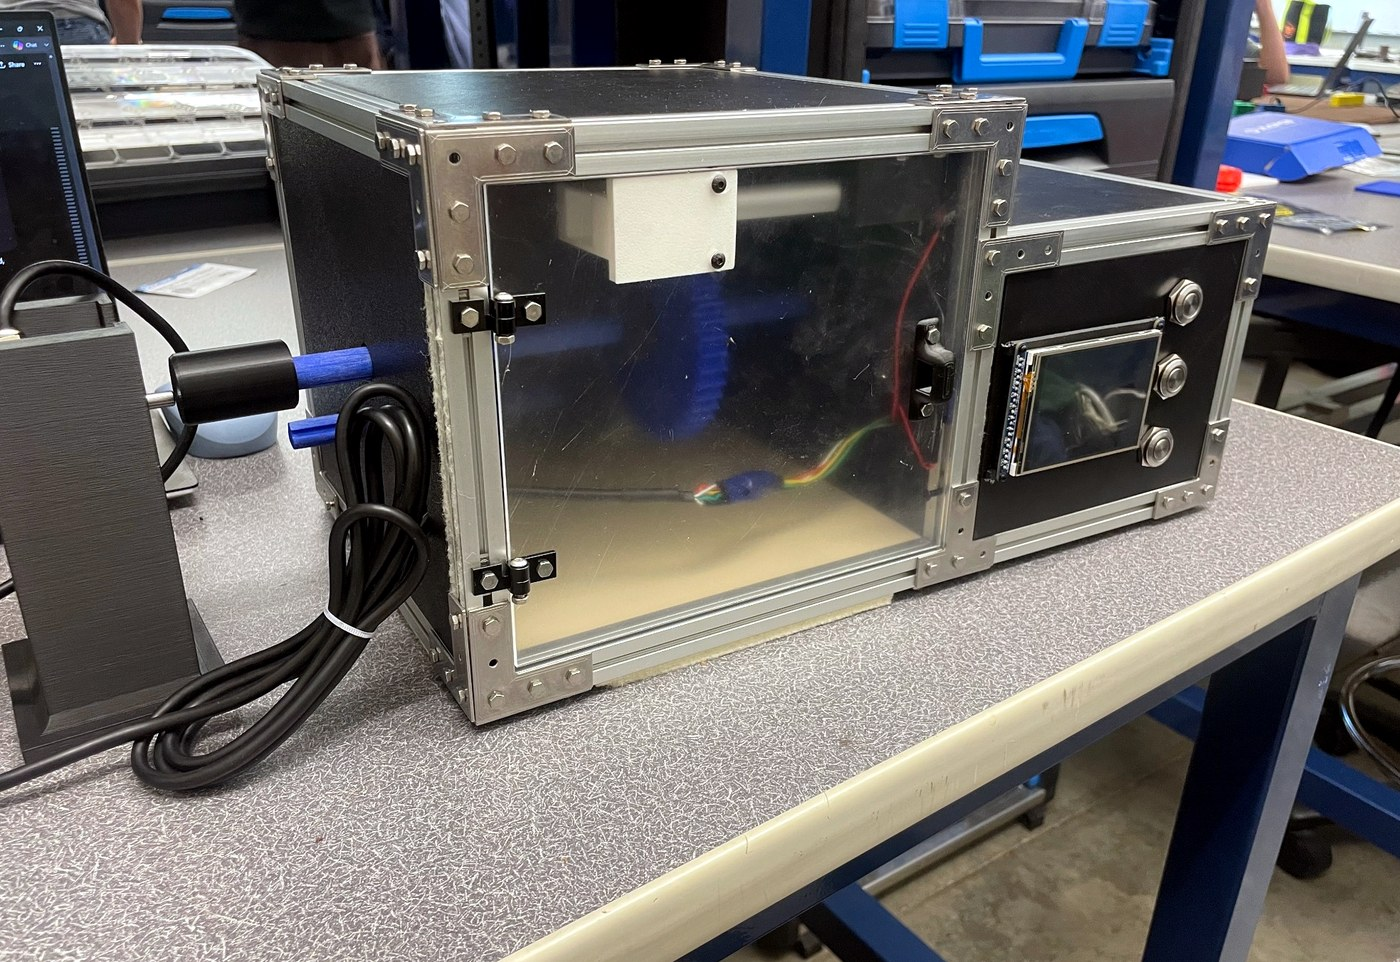
\includegraphics[
        width=5.55in,
        height=2.76in,
        keepaspectratio
    ]{prototype_overview.jpg}
};

\node[
    anchor=north,
    align=center,
    inner sep=0pt,
    text width=5.30in,
    text=Muted,
    font=\sffamily\fontsize{6.25}{6.95}\selectfont
]
at ($(current page.north west)+(7.2in,-4.46in)$)
{Completed gearbox demonstration with enclosed mechanism, TFT interface, and user controls};

% Lower section title
\node[
    anchor=north west,
    text=DeepGreen,
    font=\sffamily\bfseries\fontsize{8.0}{8.7}\selectfont
]
at ($(current page.north west)+(0.43in,-4.70in)$)
{SYSTEM DEVELOPMENT AND FINAL ARCHITECTURE};

% Lower left — CAD card
\node[
    anchor=north west,
    inner sep=2.5pt,
    draw=RuleGray,
    line width=0.55pt,
    rounded corners=5pt
]
at ($(current page.north west)+(0.42in,-4.95in)$)
{
    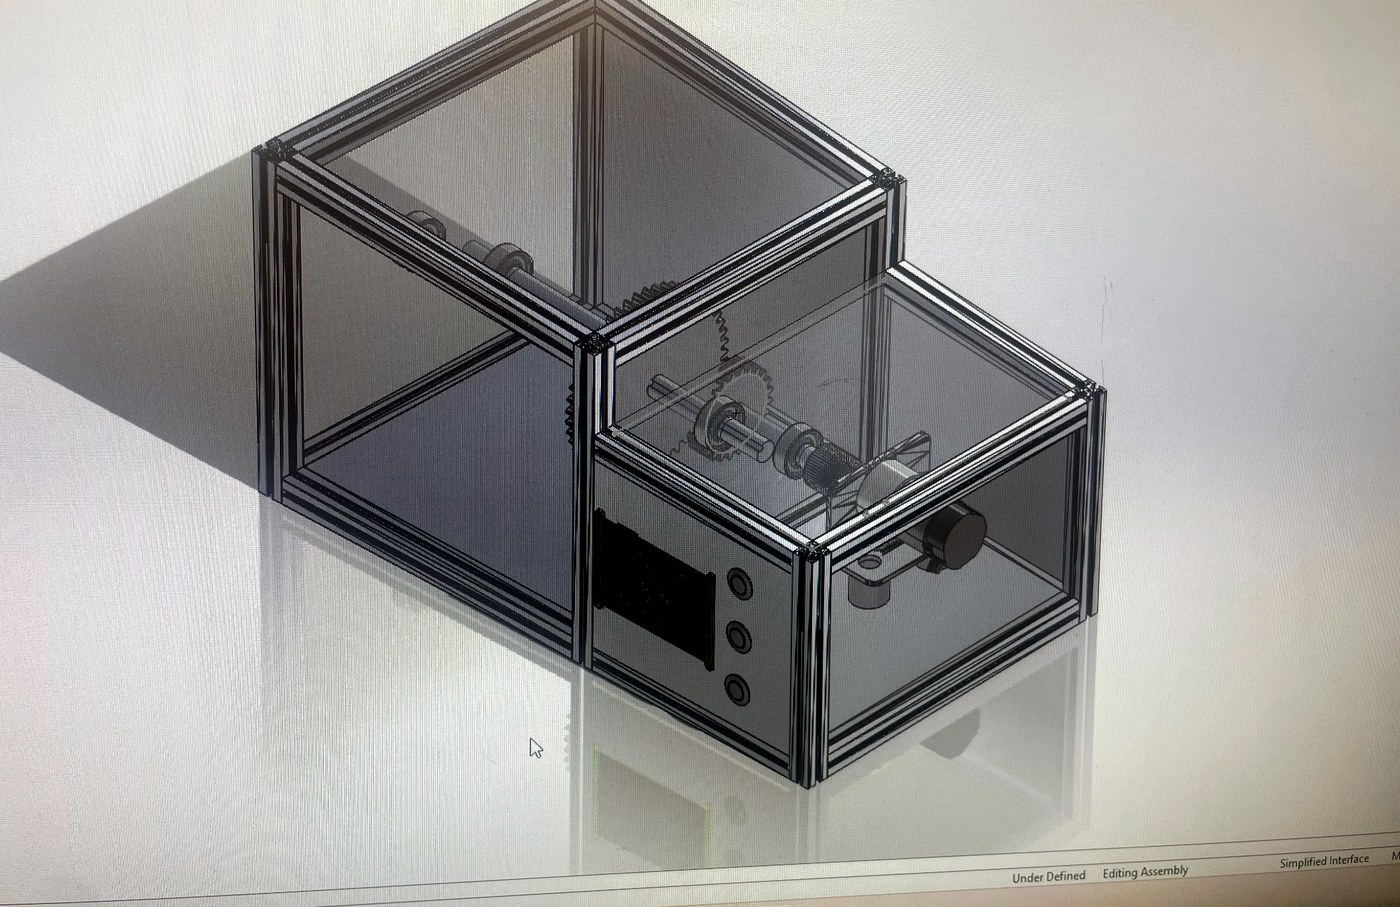
\includegraphics[
        width=2.88in,
        height=1.93in,
        keepaspectratio
    ]{cad_overview.jpg}
};

\node[
    anchor=north,
    align=center,
    inner sep=0pt,
    text width=2.72in,
    text=Muted,
    font=\sffamily\fontsize{6.05}{6.75}\selectfont
]
at ($(current page.north west)+(1.86in,-6.98in)$)
{SolidWorks packaging concept for the gearbox, enclosure, and control panel};

% Lower center — wiring diagram
\node[
    anchor=north west,
    inner sep=2.5pt,
    draw=RuleGray,
    line width=0.55pt,
    rounded corners=5pt
]
at ($(current page.north west)+(3.56in,-4.95in)$)
{
    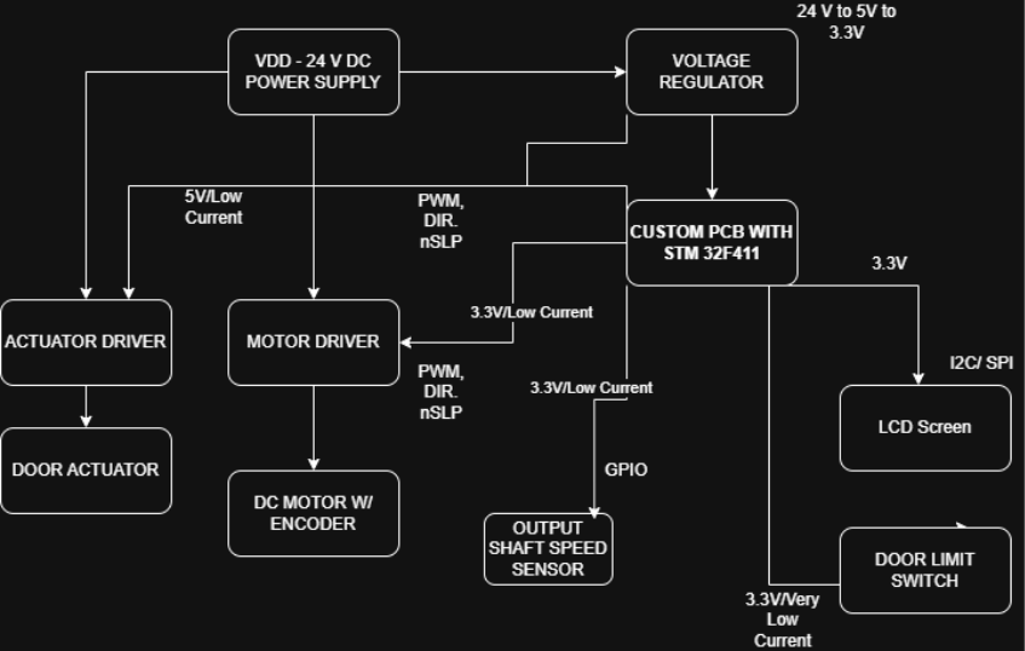
\includegraphics[
        width=3.62in,
        height=1.93in,
        keepaspectratio
    ]{WIRING_DIAGRAM.png}
};

\node[
    anchor=north,
    align=center,
    inner sep=0pt,
    text width=3.46in,
    text=Muted,
    font=\sffamily\fontsize{6.05}{6.75}\selectfont
]
at ($(current page.north west)+(5.37in,-6.98in)$)
{Power and control architecture};

% Lower right — platform highlights moved into the open space
\fill[SoftGreen,rounded corners=5pt]
    ($(current page.north west)+(6.98in,-4.95in)$)
    rectangle
    ($(current page.north east)+(-0.42in,-6.91in)$);

\draw[RuleGray,line width=0.55pt,rounded corners=5pt]
    ($(current page.north west)+(6.98in,-4.95in)$)
    rectangle
    ($(current page.north east)+(-0.42in,-6.91in)$);

\node[
    anchor=north west,
    text=DeepGreen,
    font=\sffamily\bfseries\fontsize{7.75}{8.45}\selectfont
]
at ($(current page.north west)+(7.20in,-5.14in)$)
{PLATFORM HIGHLIGHTS};

\node[
    anchor=north west,
    align=left,
    text width=3.08in,
    text=Ink,
    font=\fontsize{5.72}{6.58}\selectfont
]
at ($(current page.north west)+(7.20in,-5.43in)$)
{
\textbf{Four-layer board.}
Signals were routed on the top and bottom copper layers, with an internal 3.3 V logic plane and a dedicated ground plane.\\[4pt]

\textbf{Integrated control.}
The PCB combines dual encoder inputs, motor and actuator control, a TFT display, user buttons, USB, SWD, voltage sensing, and expansion headers.
};

% Standalone full-width centered resource bar
\fill[Panel,rounded corners=4pt]
    ($(current page.north west)+(0.42in,-7.20in)$)
    rectangle
    ($(current page.north east)+(-0.42in,-7.64in)$);

\draw[RuleGray,line width=0.5pt,rounded corners=4pt]
    ($(current page.north west)+(0.42in,-7.20in)$)
    rectangle
    ($(current page.north east)+(-0.42in,-7.64in)$);

\node[
    anchor=center,
    align=center,
    text=DeepGreen,
    font=\sffamily\bfseries\fontsize{6.75}{7.35}\selectfont
]
at ($(current page.north)+(0,-7.42in)$)
{
\href{\GearMeshVideoURL}{\faPlayCircle\ GEAR MESH DEMO}
\hspace{24pt}
\href{\GearboxSchematicOneURL}{\faFilePdf\ SCHEMATIC 1}
\hspace{24pt}
\href{\GearboxSchematicTwoURL}{\faFilePdf\ SCHEMATIC 2}
};

% Footer
\node[
    anchor=south west,
    text=white,
    font=\sffamily\bfseries\fontsize{7.1}{7.7}\selectfont
]
at ($(current page.south west)+(0.42in,0.17in)$)
{\hyperlink{mechatronics}{\faArrowLeft\ MECHATRONICS}};

\node[
    anchor=south,
    text=white,
    font=\sffamily\fontsize{7.0}{7.6}\selectfont
]
at ($(current page.south)+(0,0.17in)$)
{GEARBOX CONTROLLER \hspace{6pt} 1 / 3};

\node[
    anchor=south east,
    text=white,
    font=\sffamily\bfseries\fontsize{7.1}{7.7}\selectfont
]
at ($(current page.south east)+(-0.42in,0.17in)$)
{PCB ARCHITECTURE \faArrowRight};

\end{tikzpicture}

% ============================================================
% PAGE 2 — PCB DESIGN, ROUTING, AND MANUFACTURING
% Images used on this page:
%   pcb_render.png
%   complete_pcb.jpeg
%   Top_layer.png
%   bottom_layer.png
%   stm32_pinout.png
% Resources used on this page:
%   JLCPCB BOM
%   Pick-and-Place
%   PCB Pinout Logic
% ============================================================

\clearpage
\thispagestyle{empty}
\null

\begin{tikzpicture}[remember picture,overlay]

% Background and bars
\fill[white] (current page.south west) rectangle (current page.north east);

\fill[DeepGreen]
    (current page.north west)
    rectangle
    ($(current page.north east)+(0,-0.095in)$);

\fill[PolyGold]
    ($(current page.north west)+(0,-0.095in)$)
    rectangle
    ($(current page.north east)+(0,-0.14in)$);

\fill[DeepGreen]
    (current page.south west)
    rectangle
    ($(current page.south east)+(0,0.36in)$);

\fill[PolyGold]
    ($(current page.south west)+(0,0.36in)$)
    rectangle
    ($(current page.south east)+(0,0.405in)$);

% Header
\node[
    anchor=north west,
    text=PolyGold,
    font=\sffamily\bfseries\fontsize{8.1}{8.7}\selectfont
]
at ($(current page.north west)+(0.42in,-0.39in)$)
{GEARBOX CONTROLLER \hspace{5pt}/\hspace{5pt} PCB ARCHITECTURE};

\node[
    anchor=north west,
    text=DeepGreen,
    font=\bfseries\fontsize{21.5}{22.5}\selectfont
]
at ($(current page.north west)+(0.40in,-0.67in)$)
{FROM COMPONENT SELECTION TO MANUFACTURED BOARD};

\node[
    anchor=north west,
    text=Muted,
    font=\sffamily\fontsize{8.2}{8.95}\selectfont
]
at ($(current page.north west)+(0.42in,-1.12in)$)
{Independent circuit development, JLCPCB sourcing, multilayer routing, assembly, and embedded hardware integration};

\fill[PolyGold]
    ($(current page.north west)+(0.42in,-1.36in)$)
    rectangle
    ($(current page.north west)+(8.80in,-1.315in)$);

% Top left — populated 3D render
\node[
    anchor=north west,
    inner sep=2.6pt,
    draw=DeepGreen,
    line width=0.68pt,
    rounded corners=5pt
]
at ($(current page.north west)+(0.42in,-1.58in)$)
{
    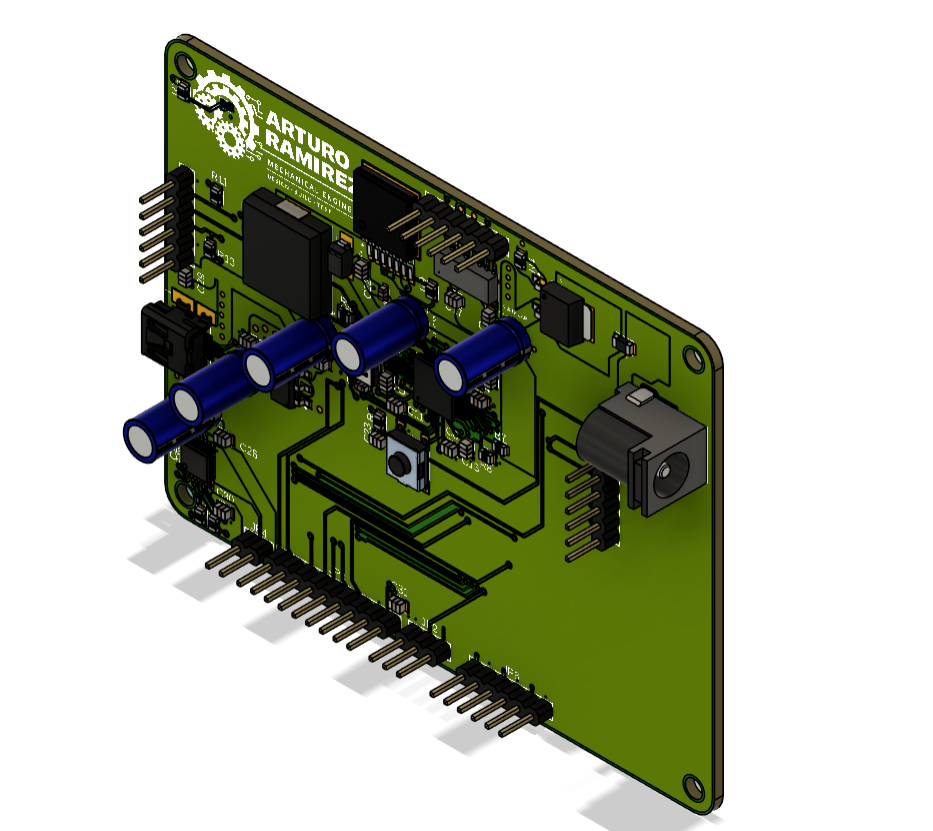
\includegraphics[
        width=3.23in,
        height=2.25in,
        keepaspectratio
    ]{pcb_render.png}
};

\node[
    anchor=north,
    align=center,
    inner sep=0pt,
    text width=3.08in,
    text=Muted,
    font=\sffamily\fontsize{6.15}{6.85}\selectfont
]
at ($(current page.north west)+(1.7in,-3.94in)$)
{Fusion 360 Electronics render of the populated controller PCB};

% Top center — fabricated PCB photograph
\node[
    anchor=north west,
    inner sep=2.6pt,
    draw=DeepGreen,
    line width=0.68pt,
    rounded corners=5pt
]
at ($(current page.north west)+(3.90in,-1.58in)$)
{
    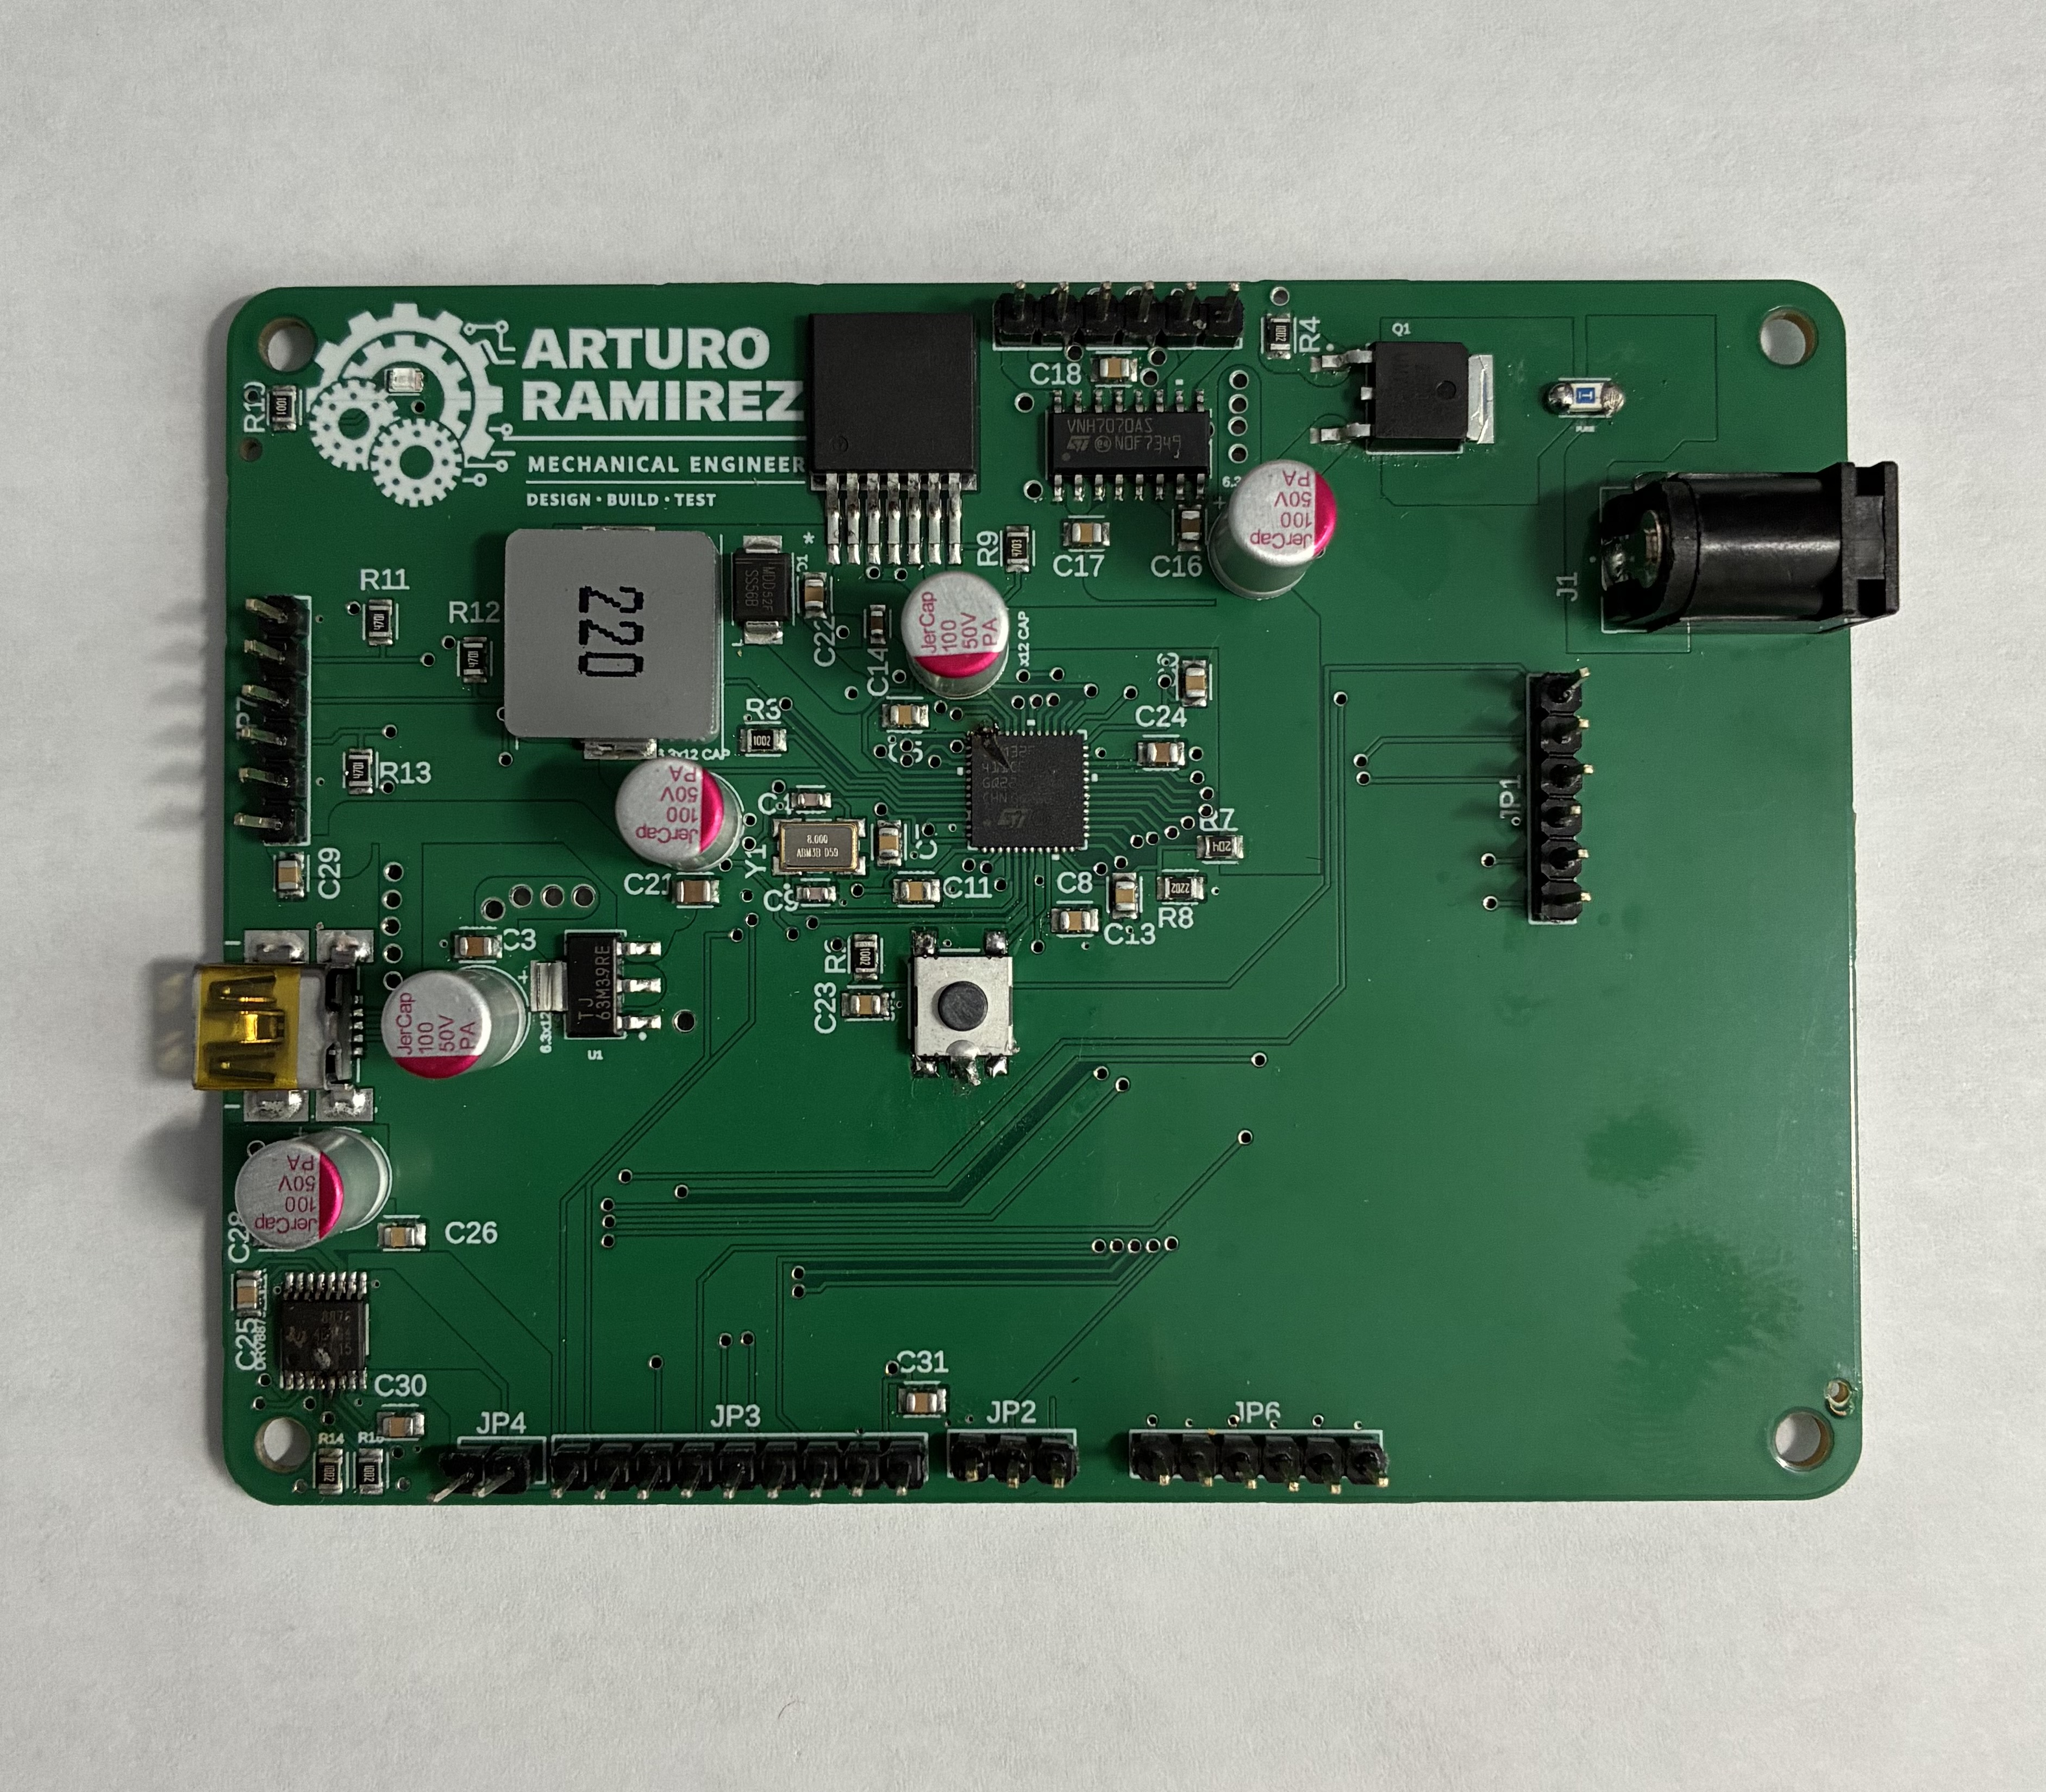
\includegraphics[
        width=3.38in,
        height=2.25in,
        keepaspectratio
    ]{complete_pcb.jpeg}
};

\node[
    anchor=north,
    align=center,
    inner sep=0pt,
    text width=3.20in,
    text=Muted,
    font=\sffamily\fontsize{6.15}{6.85}\selectfont
]
at ($(current page.north west)+(5.2in,-3.94in)$)
{Fabricated and partially populated first-generation controller PCB};

% Top right — design approach
\fill[SoftGold,rounded corners=5pt]
    ($(current page.north west)+(7.52in,-1.58in)$)
    rectangle
    ($(current page.north east)+(-0.42in,-2.71in)$);

\fill[PolyGold]
    ($(current page.north west)+(7.52in,-1.58in)$)
    rectangle
    ($(current page.north west)+(7.62in,-2.71in)$);

\node[
    anchor=north west,
    text=DeepGreen,
    font=\sffamily\bfseries\fontsize{7.8}{8.5}\selectfont
]
at ($(current page.north west)+(7.82in,-1.76in)$)
{DESIGN APPROACH};

\node[
    anchor=north west,
    align=left,
    text width=2.48in,
    text=Ink,
    font=\fontsize{5.30}{6.05}\selectfont
]
at ($(current page.north west)+(7.82in,-2.04in)$)
{
The board was developed from the system requirements outward.\\[2pt]
MCUs, drivers, regulators, connectors, passives, footprints, and
protection devices were verified against datasheets, package limits,
assembly access, and JLCPCB availability before routing.
};

% Top right — integrated features
\fill[SoftGreen,rounded corners=5pt]
    ($(current page.north west)+(7.52in,-2.91in)$)
    rectangle
    ($(current page.north east)+(-0.42in,-4.04in)$);

\draw[RuleGray,line width=0.55pt,rounded corners=5pt]
    ($(current page.north west)+(7.52in,-2.91in)$)
    rectangle
    ($(current page.north east)+(-0.42in,-4.04in)$);

\node[
    anchor=north west,
    text=DeepGreen,
    font=\sffamily\bfseries\fontsize{7.8}{8.5}\selectfont
]
at ($(current page.north west)+(7.78in,-3.09in)$)
{INTEGRATED FEATURES};

\node[
    anchor=north west,
    align=left,
    text width=2.86in,
    text=Ink,
    font=\fontsize{5.55}{6.38}\selectfont
]
at ($(current page.north west)+(7.78in,-3.37in)$)
{
STM32F411 \textbullet\ 24 V input\\
5 V buck \textbullet\ 3.3 V logic\\
Motor and actuator control\\
Dual encoder interfaces\\
SPI TFT \textbullet\ buttons \textbullet\ limit switch\\
USB \textbullet\ SWD \textbullet\ voltage sensing
};

% Routing section title
\node[
    anchor=north west,
    text=DeepGreen,
    font=\sffamily\bfseries\fontsize{8.0}{8.7}\selectfont
]
at ($(current page.north west)+(0.43in,-4.30in)$)
{ROUTING, MCU ASSIGNMENT, AND DESIGN FOR MANUFACTURING};

% Routing cards
\node[
    anchor=north west,
    inner sep=2.4pt,
    draw=RuleGray,
    line width=0.55pt,
    rounded corners=4pt
]
at ($(current page.north west)+(0.42in,-4.56in)$)
{
    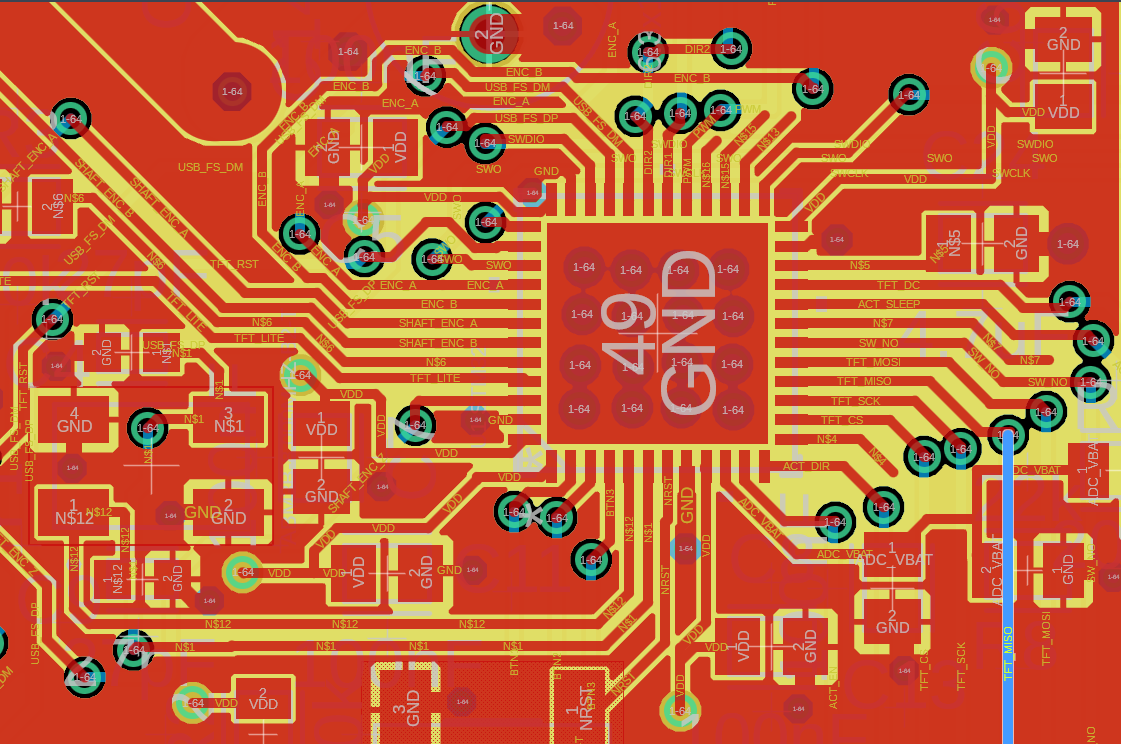
\includegraphics[
        width=3.34in,
        height=1.64in,
        keepaspectratio
    ]{Top_layer.png}
};

\node[
    anchor=north,
    align=center,
    inner sep=0pt,
    text width=3.18in,
    text=Muted,
    font=\sffamily\fontsize{6.10}{6.80}\selectfont
]
at ($(current page.north west)+(1.8in,-6.29in)$)
{Top-layer routing and component fan-out};

\node[
    anchor=north west,
    inner sep=2.4pt,
    draw=RuleGray,
    line width=0.55pt,
    rounded corners=4pt
]
at ($(current page.north west)+(3.98in,-4.56in)$)
{
    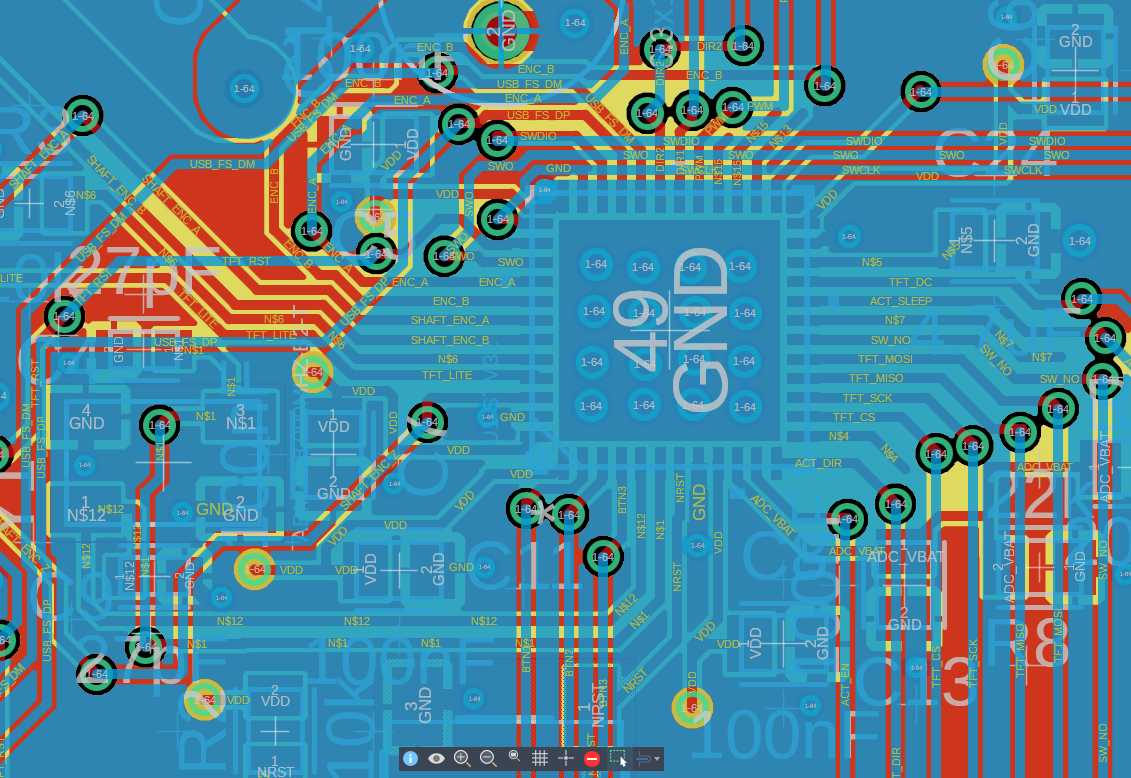
\includegraphics[
        width=3.34in,
        height=1.64in,
        keepaspectratio
    ]{bottom_layer.png}
};

\node[
    anchor=north,
    align=center,
    inner sep=0pt,
    text width=3.18in,
    text=Muted,
    font=\sffamily\fontsize{6.10}{6.80}\selectfont
]
at ($(current page.north west)+(5.3in,-6.29in)$)
{Bottom-layer routing and return-path organization};

\node[
    anchor=north west,
    inner sep=2.4pt,
    draw=RuleGray,
    line width=0.55pt,
    rounded corners=4pt
]
at ($(current page.north west)+(7.54in,-4.56in)$)
{
    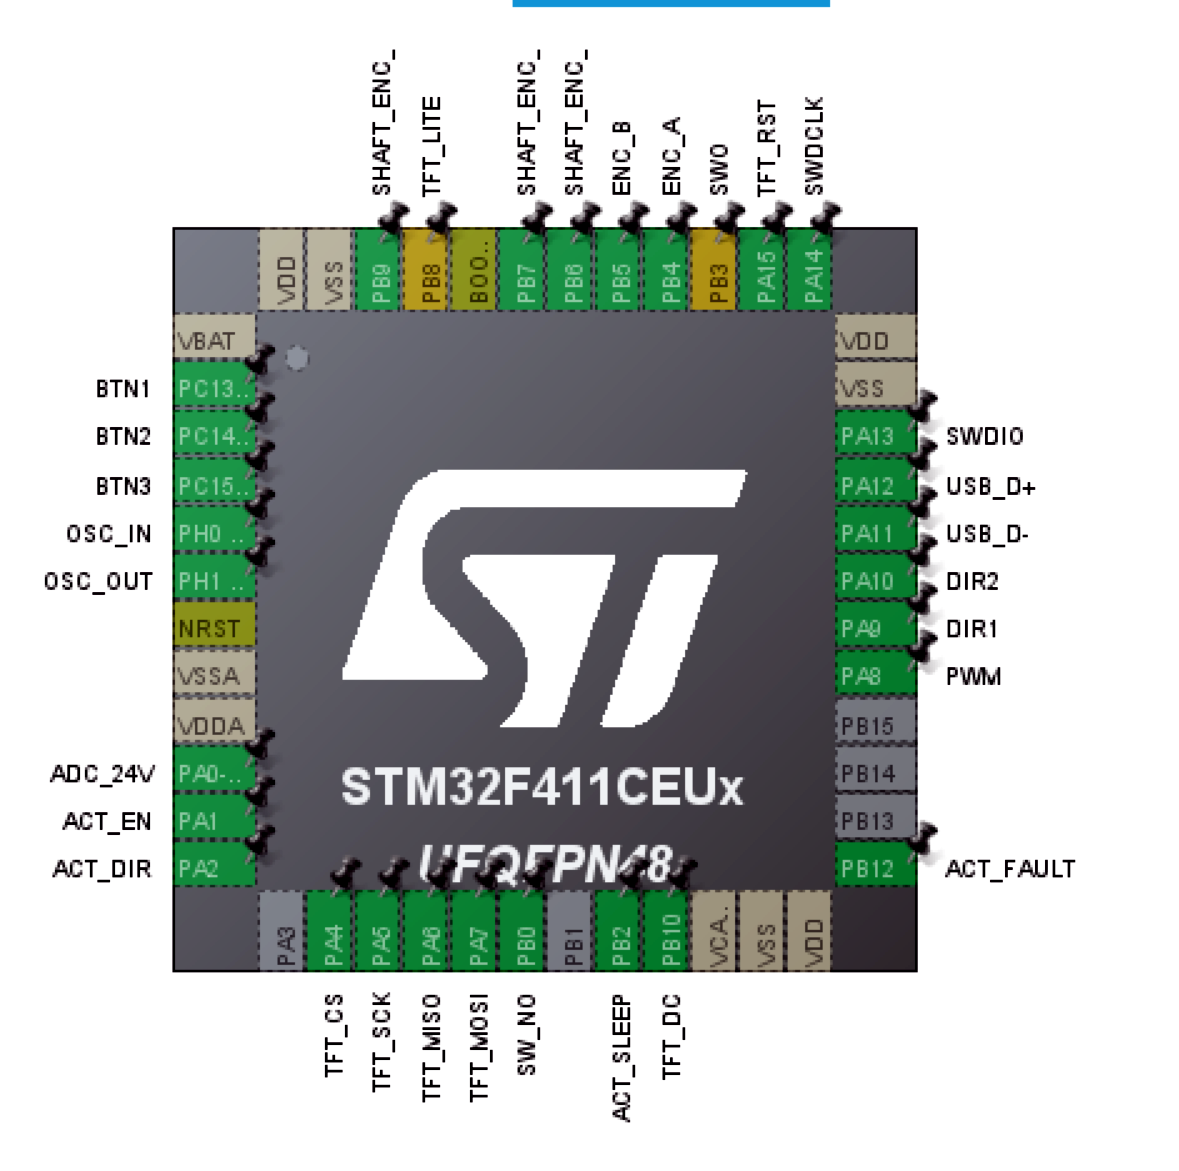
\includegraphics[
        width=3.20in,
        height=1.64in,
        keepaspectratio
    ]{stm32_pinout.png}
};

\node[
    anchor=north,
    align=center,
    inner sep=0pt,
    text width=3.04in,
    text=Muted,
    font=\sffamily\fontsize{6.10}{6.80}\selectfont
]
at ($(current page.north west)+(8.45in,-6.29in)$)
{STM32F411 GPIO and peripheral assignment};

% Bottom engineering panels
\fill[SoftGreen,rounded corners=5pt]
    ($(current page.north west)+(0.42in,-6.56in)$)
    rectangle
    ($(current page.north west)+(5.34in,-7.24in)$);

\draw[RuleGray,line width=0.55pt,rounded corners=5pt]
    ($(current page.north west)+(0.42in,-6.56in)$)
    rectangle
    ($(current page.north west)+(5.34in,-7.24in)$);

\node[
    anchor=north west,
    text=DeepGreen,
    font=\sffamily\bfseries\fontsize{7.25}{7.95}\selectfont
]
at ($(current page.north west)+(0.66in,-6.70in)$)
{POWER ARCHITECTURE};

\node[
    anchor=north west,
    align=left,
    text width=4.40in,
    text=Ink,
    font=\fontsize{6.02}{6.90}\selectfont
]
at ($(current page.north west)+(0.66in,-6.94in)$)
{
24 V motor supply \(\rightarrow\) protected input \(\rightarrow\) 5 V buck conversion
\(\rightarrow\) 3.3 V logic regulation, with local bulk and high-frequency decoupling.
};

\fill[SoftGold,rounded corners=5pt]
    ($(current page.north west)+(5.56in,-6.56in)$)
    rectangle
    ($(current page.north east)+(-0.42in,-7.24in)$);

\fill[PolyGold]
    ($(current page.north west)+(5.56in,-6.56in)$)
    rectangle
    ($(current page.north west)+(5.66in,-7.24in)$);

\node[
    anchor=north west,
    text=DeepGreen,
    font=\sffamily\bfseries\fontsize{7.25}{7.95}\selectfont
]
at ($(current page.north west)+(5.86in,-6.70in)$)
{DESIGN FOR MANUFACTURING};

\node[
    anchor=north west,
    align=left,
    text width=4.60in,
    text=Ink,
    font=\fontsize{6.00}{6.88}\selectfont
]
at ($(current page.north west)+(5.86in,-6.94in)$)
{
JLCPCB stock, assembly orientation, connector access, soldering practicality,
test access, and footprint verification directly shaped the final board.
};

% Resource links
\node[
    anchor=north,
    align=center,
    text=DeepGreen,
    font=\sffamily\bfseries\fontsize{6.75}{7.35}\selectfont
]
at ($(current page.north)+(0,-7.45in)$)
{
\href{\GearboxBOMURL}{\faFilePdf\ JLCPCB BOM}
\hspace{18pt}
\href{\GearboxPnPURL}{\faFilePdf\ PICK-AND-PLACE}
\hspace{18pt}
\href{\GearboxPinoutURL}{\faFilePdf\ PCB PINOUT LOGIC}
};

% Footer
\node[
    anchor=south west,
    text=white,
    font=\sffamily\bfseries\fontsize{7.1}{7.7}\selectfont
]
at ($(current page.south west)+(0.42in,0.17in)$)
{\faArrowLeft\ SYSTEM OVERVIEW};

\node[
    anchor=south,
    text=white,
    font=\sffamily\fontsize{7.0}{7.6}\selectfont
]
at ($(current page.south)+(0,0.17in)$)
{GEARBOX CONTROLLER \hspace{6pt} 2 / 3};

\node[
    anchor=south east,
    text=white,
    font=\sffamily\bfseries\fontsize{7.1}{7.7}\selectfont
]
at ($(current page.south east)+(-0.42in,0.17in)$)
{INTEGRATION \& TAKEAWAYS \faArrowRight};

\end{tikzpicture}

% ============================================================
% PAGE 3 — EMBEDDED INTEGRATION, LESSONS, AND FUTURE PLATFORM
% Image used on this page:
%   pcb_layer_view.png
% No Google Drive resource is repeated on this page.
% ============================================================

\clearpage
\thispagestyle{empty}
\null

\begin{tikzpicture}[remember picture,overlay]

% Background and bars
\fill[white] (current page.south west) rectangle (current page.north east);

\fill[DeepGreen]
    (current page.north west)
    rectangle
    ($(current page.north east)+(0,-0.095in)$);

\fill[PolyGold]
    ($(current page.north west)+(0,-0.095in)$)
    rectangle
    ($(current page.north east)+(0,-0.14in)$);

\fill[DeepGreen]
    (current page.south west)
    rectangle
    ($(current page.south east)+(0,0.36in)$);

\fill[PolyGold]
    ($(current page.south west)+(0,0.36in)$)
    rectangle
    ($(current page.south east)+(0,0.405in)$);

% Header
\node[
    anchor=north west,
    text=PolyGold,
    font=\sffamily\bfseries\fontsize{8.1}{8.7}\selectfont
]
at ($(current page.north west)+(0.42in,-0.39in)$)
{GEARBOX CONTROLLER \hspace{5pt}/\hspace{5pt} INTEGRATION AND ENGINEERING TAKEAWAYS};

\node[
    anchor=north west,
    text=DeepGreen,
    font=\bfseries\fontsize{22.0}{23.0}\selectfont
]
at ($(current page.north west)+(0.40in,-0.67in)$)
{A REUSABLE PLATFORM FOR EMBEDDED CONTROL};

\node[
    anchor=north west,
    text=Muted,
    font=\sffamily\fontsize{8.25}{9.0}\selectfont
]
at ($(current page.north west)+(0.42in,-1.12in)$)
{Hardware assembly, CubeMX configuration, collaborative firmware development, and next-generation expansion};

\fill[PolyGold]
    ($(current page.north west)+(0.42in,-1.36in)$)
    rectangle
    ($(current page.north west)+(8.82in,-1.315in)$);

% Large PCB routing image — only use of this image
\node[
    anchor=north west,
    inner sep=2.6pt,
    draw=DeepGreen,
    line width=0.68pt,
    rounded corners=5pt
]
at ($(current page.north west)+(0.42in,-1.58in)$)
{
    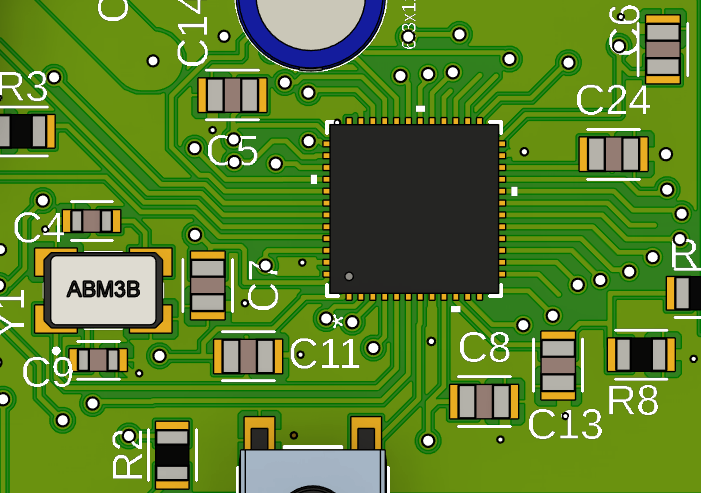
\includegraphics[
        width=5.20in,
        height=3.15in,
        keepaspectratio
    ]{pcb_layer_view.png}
};

\node[
    anchor=north,
    align=center,
    inner sep=0pt,
    text width=4.98in,
    text=Muted,
    font=\sffamily\fontsize{6.30}{7.00}\selectfont
]
at ($(current page.north west)+(3.02in,-4.85in)$)
{Dense MCU breakout, encoder routing, SWD, USB, TFT, actuator, and sensing interfaces};

% Top right — hardware and firmware integration
% Left edge aligned with the Future Learning Platform panel below.
\fill[SoftGold,rounded corners=5pt]
    ($(current page.north west)+(5.56in,-1.58in)$)
    rectangle
    ($(current page.north east)+(-0.42in,-4.92in)$);

\fill[PolyGold]
    ($(current page.north west)+(5.56in,-1.58in)$)
    rectangle
    ($(current page.north west)+(5.66in,-4.92in)$);

\node[
    anchor=north west,
    text=DeepGreen,
    font=\sffamily\bfseries\fontsize{8.0}{8.7}\selectfont
]
at ($(current page.north west)+(5.86in,-1.77in)$)
{HARDWARE AND FIRMWARE INTEGRATION};

\node[
    anchor=north west,
    align=left,
    text width=4.54in,
    text=Ink,
    font=\fontsize{6.65}{7.78}\selectfont
]
at ($(current page.north west)+(5.86in,-2.07in)$)
{
After fabrication, I soldered the selected components and integrated the
PCB into the larger system architecture. My partner and I jointly configured
the STM32 in CubeMX to establish clocking, GPIO, timers, encoder inputs,
SPI communication, USB, and debug access.\\[5pt]

We developed the firmware around collaborative multitasking in C/C++ so
that motor control, display updates, user commands, actuator behavior, and
safety logic could operate as one cohesive controller rather than as isolated
demonstrations.\\[5pt]

This first revision served as a functional learning platform while exposing
practical improvements for protection, test access, connector planning,
packaging, and future instrumentation.
};

% Bottom left — engineering takeaways
\fill[SoftGreen,rounded corners=5pt]
    ($(current page.north west)+(0.42in,-5.18in)$)
    rectangle
    ($(current page.north west)+(5.34in,-7.30in)$);

\draw[RuleGray,line width=0.55pt,rounded corners=5pt]
    ($(current page.north west)+(0.42in,-5.18in)$)
    rectangle
    ($(current page.north west)+(5.34in,-7.30in)$);

\node[
    anchor=north west,
    text=DeepGreen,
    font=\sffamily\bfseries\fontsize{7.8}{8.5}\selectfont
]
at ($(current page.north west)+(0.68in,-5.36in)$)
{ENGINEERING TAKEAWAYS};

\node[
    anchor=north west,
    align=left,
    text width=4.42in,
    text=Ink,
    font=\fontsize{6.25}{7.25}\selectfont
]
at ($(current page.north west)+(0.68in,-5.65in)$)
{
\textbf{Architecture first.}
Defining interfaces before routing reduced late-stage changes and simplified integration.\\[4pt]

\textbf{Datasheets are the design language.}
Selection required verifying voltage, current, package, thermal, and control requirements rather than relying on names alone.\\[4pt]

\textbf{Manufacturability shapes electronics.}
Stock, assembly, access, solderability, and testability directly influenced the final circuit.\\[4pt]

\textbf{First revisions are learning tools.}
Bring-up revealed improvements for protection, debug access, and packaging.
};

% Bottom right — future platform
\fill[SoftGold,rounded corners=5pt]
    ($(current page.north west)+(5.56in,-5.18in)$)
    rectangle
    ($(current page.north east)+(-0.42in,-7.30in)$);

\fill[PolyGold]
    ($(current page.north west)+(5.56in,-5.18in)$)
    rectangle
    ($(current page.north west)+(5.66in,-7.30in)$);

\node[
    anchor=north west,
    text=DeepGreen,
    font=\sffamily\bfseries\fontsize{7.8}{8.5}\selectfont
]
at ($(current page.north west)+(5.86in,-5.36in)$)
{FUTURE LEARNING PLATFORM};

\node[
    anchor=north west,
    align=left,
    text width=4.58in,
    text=Ink,
    font=\fontsize{6.25}{7.25}\selectfont
]
at ($(current page.north west)+(5.86in,-5.65in)$)
{
The controller was intentionally conceived as more than a single-purpose
gearbox driver. Future revisions can add torque sensing, motor-current
measurement, temperature monitoring, improved output-speed sensing,
and additional analog or digital sensors.\\[5pt]

Those additions would support system identification, efficiency studies,
closed-loop speed control, comparison between predicted and measured
gear ratios, and the development of kinetic as well as kinematic models.
The existing PCB, enclosure, display, and modular mechanical platform
provide the foundation for those experiments.
};

% Footer
\node[
    anchor=south west,
    text=white,
    font=\sffamily\bfseries\fontsize{7.1}{7.7}\selectfont
]
at ($(current page.south west)+(0.42in,0.17in)$)
{\faArrowLeft\ PCB ARCHITECTURE};

\node[
    anchor=south,
    text=white,
    font=\sffamily\fontsize{7.0}{7.6}\selectfont
]
at ($(current page.south)+(0,0.17in)$)
{GEARBOX CONTROLLER \hspace{6pt} 3 / 3};

\node[
    anchor=south east,
    text=white,
    font=\sffamily\bfseries\fontsize{7.1}{7.7}\selectfont
]
at ($(current page.south east)+(-0.42in,0.17in)$)
{NEXT PROJECT \faArrowRight};

\end{tikzpicture}

\input{romi}
\clearpage

% First project in the section
\clearpage

\clearpage


% =========================
% Mechatronics Section
% =========================
% mech.tex must contain on its opening page:
% \hypertarget{mechatronics}{}
%==============================================================
% MECHATRONICS DIVIDER PAGE
%==============================================================

\clearpage
\thispagestyle{empty}
\hypertarget{mechatronics}{}

\begin{tikzpicture}[remember picture,overlay]

%--------------------------------------------------------------
% Background
%--------------------------------------------------------------

\fill[white]
(current page.south west)
rectangle
(current page.north east);

% Top bar

\fill[DeepGreen]
(current page.north west)
rectangle
($(current page.north east)+(0,-0.10in)$);

\fill[PolyGold]
($(current page.north west)+(0,-0.10in)$)
rectangle
($(current page.north east)+(0,-0.14in)$);

% Bottom bar

\fill[DeepGreen]
(current page.south west)
rectangle
($(current page.south east)+(0,0.36in)$);

\fill[PolyGold]
($(current page.south west)+(0,0.36in)$)
rectangle
($(current page.south east)+(0,0.40in)$);

%--------------------------------------------------------------
% Large section number
%--------------------------------------------------------------

\node[
anchor=north west,
text=SoftGreen,
font=\bfseries\fontsize{96}{96}\selectfont
]
at ($(current page.north west)+(0.70in,-0.90in)$)
{02};

%--------------------------------------------------------------
% Section Title
%--------------------------------------------------------------

\node[
anchor=north west,
text=DeepGreen,
font=\bfseries\fontsize{30}{32}\selectfont
]
at ($(current page.north west)+(2.15in,-1.05in)$)
{MECHATRONICS};

%--------------------------------------------------------------
% Subtitle
%--------------------------------------------------------------

\node[
anchor=north west,
text=PolyGold,
font=\sffamily\bfseries\fontsize{10}{11}\selectfont
]
at ($(current page.north west)+(2.18in,-1.62in)$)
{Embedded Systems \& Robotic Control};

% Gold rule

\fill[PolyGold]
($(current page.north west)+(2.20in,-1.83in)$)
rectangle
($(current page.north west)+(4.8in,-1.79in)$);

%--------------------------------------------------------------
% Description
%--------------------------------------------------------------

\node[
anchor=north west,
align=left,
text width=6.65in,
font=\fontsize{12}{15}\selectfont,
text=Ink
]
at ($(current page.north west)+(2.18in,-2.05in)$)
{
This section presents mechatronic systems that combine custom electronics,
embedded programming, sensing, feedback control, robotic motion, and
hardware--software integration. The projects emphasize complete system
development from circuit and mechanism design through implementation,
testing, diagnosis, and refinement.
};

%--------------------------------------------------------------
% Project Roadmap
%--------------------------------------------------------------

\node[
anchor=north west,
text=DeepGreen,
font=\sffamily\bfseries\fontsize{11}{12}\selectfont
]
at ($(current page.north west)+(2.18in,-3.25in)$)
{PROJECTS};

\node[
anchor=north west,
align=left,
text width=7.35in,
font=\fontsize{13}{20}\selectfont,
text=Ink
]
at ($(current page.north west)+(2.18in,-3.60in)$)
{

\textcolor{PolyGold}{\textbf{06}}
\hspace{0.15in}
Custom Gearbox Control PCB

\vspace{0.18in}

\textcolor{PolyGold}{\textbf{07}}
\hspace{0.15in}
Romi Autonomous Differential-Drive Robot

\vspace{0.18in}

\textcolor{PolyGold}{\textbf{08}}
\hspace{0.15in}
Kinect-Guided Autonomous Drone

\vspace{0.18in}

\textcolor{PolyGold}{\textbf{09}}
\hspace{0.15in}
Assembly Programming, FSMs \& Hardware Interaction

\vspace{0.18in}

\textcolor{PolyGold}{\textbf{10}}
\hspace{0.15in}
Robotics Methods: Vision, Kinematics \& Trajectory Planning

};

%--------------------------------------------------------------
% Navigation
%--------------------------------------------------------------

\node[
anchor=south west,
text=DeepGreen,
font=\sffamily\bfseries\fontsize{10}{11}\selectfont
]
at ($(current page.south west)+(0.70in,0.65in)$)
{\hyperlink{overview}{\faArrowLeft\ Portfolio Overview}};

\node[
anchor=south east,
text=DeepGreen,
font=\sffamily\bfseries\fontsize{10}{11}\selectfont
]
at ($(current page.south east)+(-0.70in,0.65in)$)
{\hyperlink{gearboxpcb}{Custom Gearbox Control PCB \faArrowRight}};

%--------------------------------------------------------------
% Footer
%--------------------------------------------------------------

\node[
anchor=east,
text=white,
font=\sffamily\fontsize{8}{9}\selectfont
]
at ($(current page.south east)+(-0.45in,0.18in)$)
{02 MECHATRONICS};

\end{tikzpicture}
%==============================================================
% PROJECT 06 — CUSTOM GEARBOX CONTROLLER PCB
% Three-page Mechatronics Portfolio Feature
%==============================================================

% Required image files in the Overleaf project:
% prototype_overview.jpg, cad_overview.jpg, pcb_render.png,
% Top_layer.png, bottom_layer.png, stm32_pinout.png, pcb_layer_view.png

\newcommand{\GearMeshVideoURL}{https://drive.google.com/file/d/1c9Dpt7rh-xMqnXRiqxy8QwGIDzVrn4yP/view?usp=drive_link}
\newcommand{\GearboxBOMURL}{https://drive.google.com/file/d/1r9MuhYR57b-BE1TgPTJExPTuizmPRoin/view?usp=drive_link}
\newcommand{\GearboxPnPURL}{https://drive.google.com/file/d/1twTr6gidxc5jp6XXtx9B64dvdXTclb1i/view?usp=drive_link}
\newcommand{\GearboxSchematicOneURL}{https://drive.google.com/file/d/1M6LuV9WgP7C7Q2sWUGcvKPZqV96tMXaU/view?usp=drive_link}
\newcommand{\GearboxSchematicTwoURL}{https://drive.google.com/file/d/1DglJlnw1rp7rtF8z4b_QAwdovFRx10xd/view?usp=drive_link}
\newcommand{\GearboxPinoutURL}{https://drive.google.com/file/d/1iSpHgZ1y8BdRfjCNocFGtaumFrspBP6K/view?usp=drive_link}

% ============================================================
% CUSTOM GEARBOX CONTROLLER PCB
% THREE-PAGE PORTFOLIO CASE STUDY
% 02 Mechatronics / Project 06
%
% IMPORTANT:
% 1. This file must NOT contain \documentclass, \begin{document},
%    or \end{document}.
% 2. This script assumes the main portfolio preamble already defines:
%       DeepGreen, PolyGold, SoftGold, SoftGreen,
%       RuleGray, Muted, Ink, Panel
%    and loads tikz, graphicx, hyperref, and fontawesome5.
% 3. Each image and each Google Drive resource is used exactly once.
% 4. Upload these files to Overleaf with the exact same names:
%       prototype_overview.jpg
%       cad_overview.jpg
%       pcb_render.png
%       Top_layer.png
%       bottom_layer.png
%       stm32_pinout.png
%       pcb_layer_view.png
%       WIRING_DIAGRAM.png
% ============================================================

% ============================================================
% PAGE 1 — PROJECT OVERVIEW, OWNERSHIP, AND SYSTEM ARCHITECTURE
% Images used on this page:
%   prototype_overview.jpg
%   cad_overview.jpg
%   WIRING_DIAGRAM.png
% Resources used on this page:
%   Gear Mesh Demo
%   Schematic 1
%   Schematic 2
% ============================================================

\clearpage
\thispagestyle{empty}
\hypertarget{gearboxpcb}{}
\null

\begin{tikzpicture}[remember picture,overlay]

% Background and page bars
\fill[white] (current page.south west) rectangle (current page.north east);

\fill[DeepGreen]
    (current page.north west)
    rectangle
    ($(current page.north east)+(0,-0.095in)$);

\fill[PolyGold]
    ($(current page.north west)+(0,-0.095in)$)
    rectangle
    ($(current page.north east)+(0,-0.14in)$);

\fill[DeepGreen]
    (current page.south west)
    rectangle
    ($(current page.south east)+(0,0.36in)$);

\fill[PolyGold]
    ($(current page.south west)+(0,0.36in)$)
    rectangle
    ($(current page.south east)+(0,0.405in)$);

% Header
\node[
    anchor=north west,
    text=PolyGold,
    font=\sffamily\bfseries\fontsize{8.1}{8.7}\selectfont
]
at ($(current page.north west)+(0.42in,-0.39in)$)
{02 MECHATRONICS \hspace{5pt}/\hspace{5pt} PROJECT 06};

\node[
    anchor=north west,
    text=DeepGreen,
    font=\bfseries\fontsize{22.5}{23.5}\selectfont
]
at ($(current page.north west)+(0.40in,-0.67in)$)
{CUSTOM GEARBOX CONTROLLER PCB};

\node[
    anchor=north west,
    text=Muted,
    font=\sffamily\fontsize{8.35}{9.1}\selectfont
]
at ($(current page.north west)+(0.42in,-1.12in)$)
{Cal Poly Mechatronics Laboratory \hspace{7pt}\textbullet\hspace{7pt}
Team Project \hspace{7pt}\textbullet\hspace{7pt}
Spring 2026 \hspace{7pt}\textbullet\hspace{7pt}
San Luis Obispo, California};

\fill[PolyGold]
    ($(current page.north west)+(0.42in,-1.36in)$)
    rectangle
    ($(current page.north west)+(6.in,-1.315in)$);

% Upper left — challenge
\node[
    anchor=north west,
    text=DeepGreen,
    font=\sffamily\bfseries\fontsize{8.1}{8.8}\selectfont
]
at ($(current page.north west)+(0.43in,-1.60in)$)
{THE CHALLENGE};

\node[
    anchor=north west,
    align=left,
    text width=4.42in,
    text=Ink,
    font=\fontsize{7.35}{8.70}\selectfont
]
at ($(current page.north west)+(0.43in,-1.84in)$)
{
Transform a passive gearbox demonstration into a dynamic,
interactive mechatronic platform capable of motor actuation,
encoder feedback, user input, display output, and safe enclosure
operation. The controller also needed to remain expandable for
future sensing, controls, and system-identification experiments.
};

% Upper-left role box
\fill[SoftGold,rounded corners=5pt]
    ($(current page.north west)+(0.42in,-2.70in)$)
    rectangle
    ($(current page.north west)+(4.98in,-4.40in)$);

\fill[PolyGold]
    ($(current page.north west)+(0.42in,-2.70in)$)
    rectangle
    ($(current page.north west)+(0.52in,-4.40in)$);

\node[
    anchor=north west,
    text=DeepGreen,
    font=\sffamily\bfseries\fontsize{8.0}{8.7}\selectfont
]
at ($(current page.north west)+(0.66in,-2.88in)$)
{MY ROLE — PCB DESIGNER \& ELECTRONICS LEAD};

\node[
    anchor=north west,
    align=left,
    text width=4.00in,
    text=Ink,
    font=\fontsize{6.10}{7.02}\selectfont
]
at ($(current page.north west)+(0.66in,-3.16in)$)
{
\textbullet\ Defined the controller architecture and selected the feature set\\[1.0pt]
\textbullet\ Sourced and verified components from the JLCPCB catalog\\[1.0pt]
\textbullet\ Developed the schematic, four-layer PCB, BOM, and PnP files\\[1.0pt]
\textbullet\ Routed signals on the top and bottom copper layers\\[1.0pt]
\textbullet\ Added an internal 3.3 V logic plane and dedicated ground plane\\[1.0pt]
\textbullet\ Soldered selected hardware and supported board bring-up\\[2.3pt]

\textbf{Shared integration.}
My partner and I configured CubeMX and developed the C/C++ multitasking structure.
He also led the mechanical gearbox, frame, printed shafts, collars, couplers,
keyed features, embedded bearings, acrylic door, and actuator/encoder mounts.
};

% Upper right — large prototype
\node[
    anchor=north west,
    inner sep=2.6pt,
    draw=DeepGreen,
    line width=0.68pt,
    rounded corners=6pt
]
at ($(current page.north west)+(5.18in,-1.58in)$)
{
    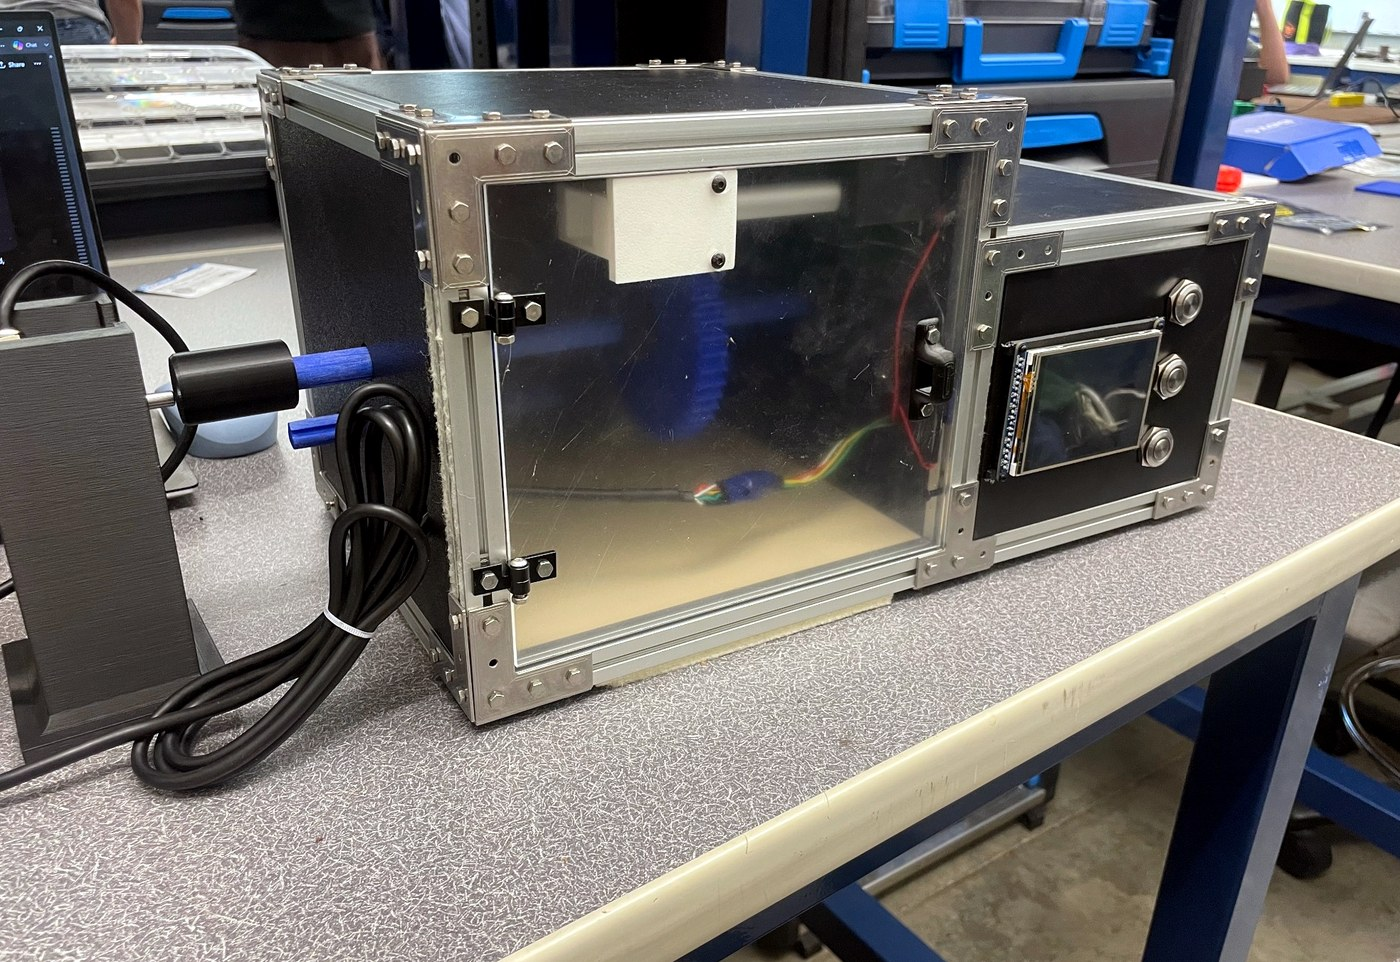
\includegraphics[
        width=5.55in,
        height=2.76in,
        keepaspectratio
    ]{prototype_overview.jpg}
};

\node[
    anchor=north,
    align=center,
    inner sep=0pt,
    text width=5.30in,
    text=Muted,
    font=\sffamily\fontsize{6.25}{6.95}\selectfont
]
at ($(current page.north west)+(7.2in,-4.46in)$)
{Completed gearbox demonstration with enclosed mechanism, TFT interface, and user controls};

% Lower section title
\node[
    anchor=north west,
    text=DeepGreen,
    font=\sffamily\bfseries\fontsize{8.0}{8.7}\selectfont
]
at ($(current page.north west)+(0.43in,-4.70in)$)
{SYSTEM DEVELOPMENT AND FINAL ARCHITECTURE};

% Lower left — CAD card
\node[
    anchor=north west,
    inner sep=2.5pt,
    draw=RuleGray,
    line width=0.55pt,
    rounded corners=5pt
]
at ($(current page.north west)+(0.42in,-4.95in)$)
{
    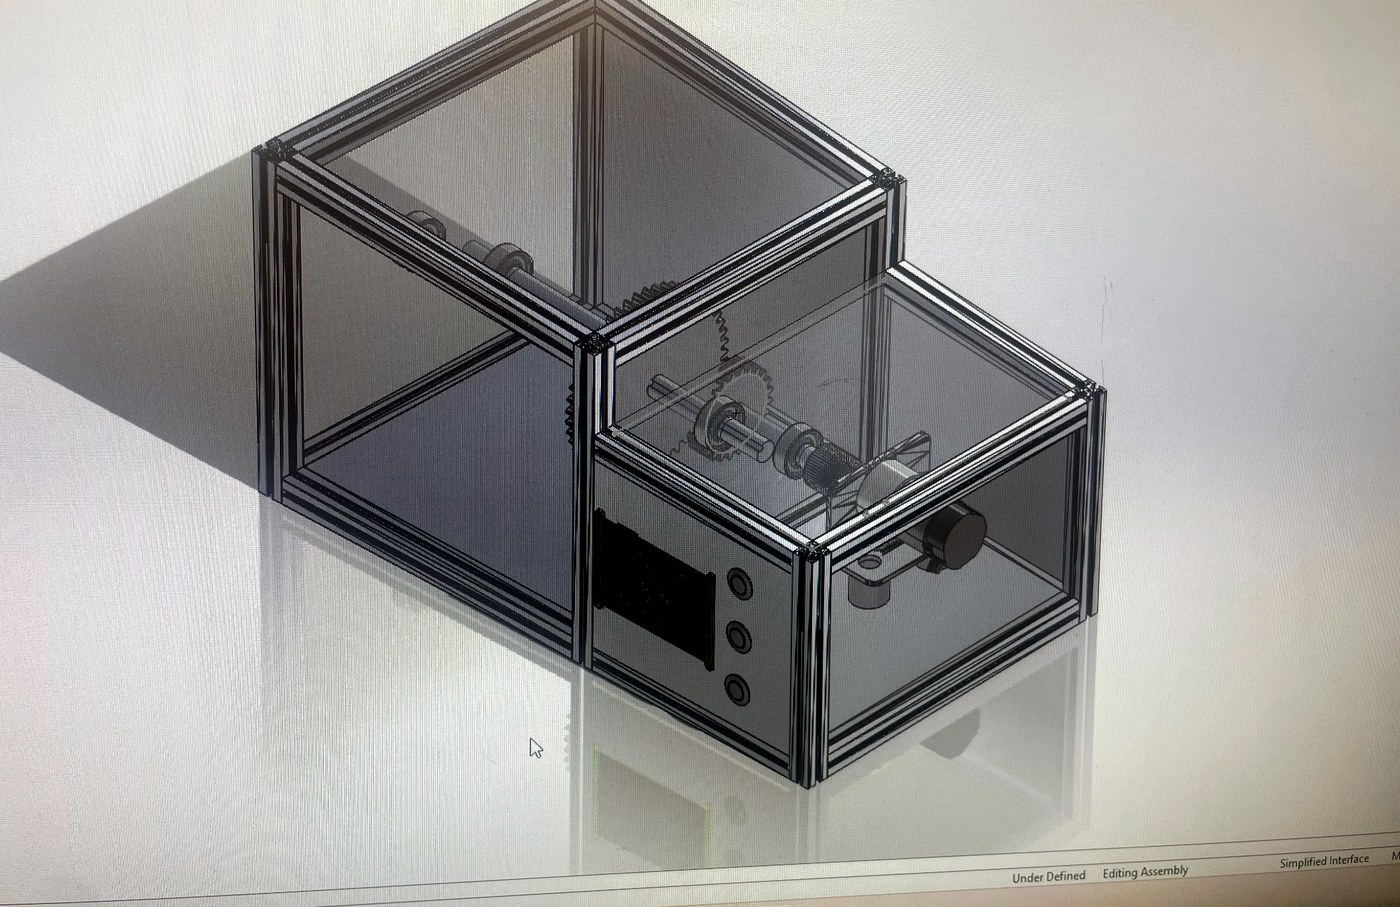
\includegraphics[
        width=2.88in,
        height=1.93in,
        keepaspectratio
    ]{cad_overview.jpg}
};

\node[
    anchor=north,
    align=center,
    inner sep=0pt,
    text width=2.72in,
    text=Muted,
    font=\sffamily\fontsize{6.05}{6.75}\selectfont
]
at ($(current page.north west)+(1.86in,-6.98in)$)
{SolidWorks packaging concept for the gearbox, enclosure, and control panel};

% Lower center — wiring diagram
\node[
    anchor=north west,
    inner sep=2.5pt,
    draw=RuleGray,
    line width=0.55pt,
    rounded corners=5pt
]
at ($(current page.north west)+(3.56in,-4.95in)$)
{
    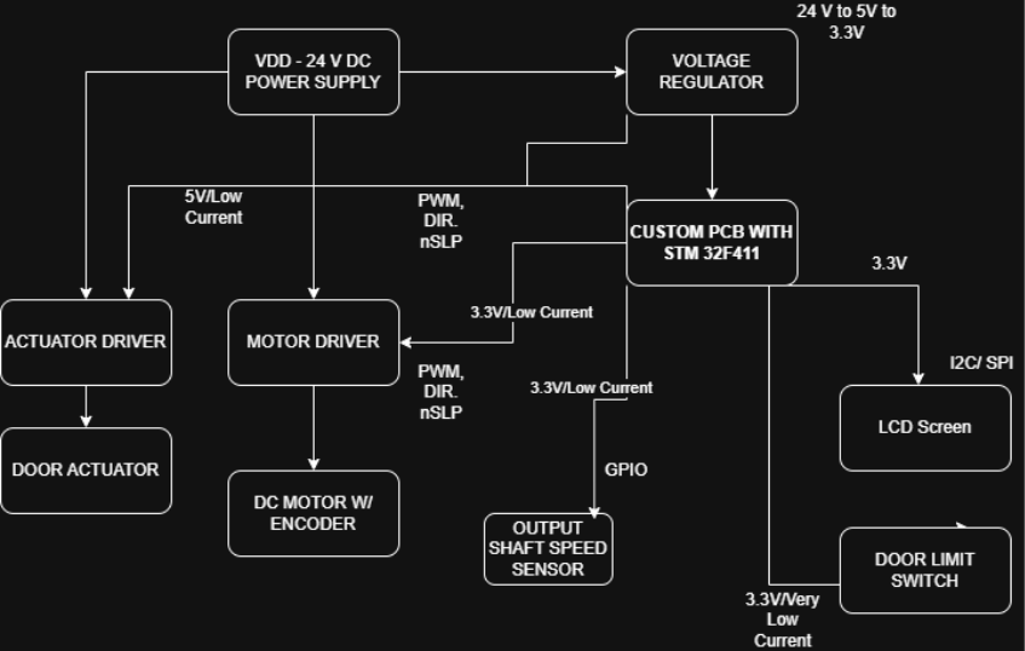
\includegraphics[
        width=3.62in,
        height=1.93in,
        keepaspectratio
    ]{WIRING_DIAGRAM.png}
};

\node[
    anchor=north,
    align=center,
    inner sep=0pt,
    text width=3.46in,
    text=Muted,
    font=\sffamily\fontsize{6.05}{6.75}\selectfont
]
at ($(current page.north west)+(5.37in,-6.98in)$)
{Power and control architecture};

% Lower right — platform highlights moved into the open space
\fill[SoftGreen,rounded corners=5pt]
    ($(current page.north west)+(6.98in,-4.95in)$)
    rectangle
    ($(current page.north east)+(-0.42in,-6.91in)$);

\draw[RuleGray,line width=0.55pt,rounded corners=5pt]
    ($(current page.north west)+(6.98in,-4.95in)$)
    rectangle
    ($(current page.north east)+(-0.42in,-6.91in)$);

\node[
    anchor=north west,
    text=DeepGreen,
    font=\sffamily\bfseries\fontsize{7.75}{8.45}\selectfont
]
at ($(current page.north west)+(7.20in,-5.14in)$)
{PLATFORM HIGHLIGHTS};

\node[
    anchor=north west,
    align=left,
    text width=3.08in,
    text=Ink,
    font=\fontsize{5.72}{6.58}\selectfont
]
at ($(current page.north west)+(7.20in,-5.43in)$)
{
\textbf{Four-layer board.}
Signals were routed on the top and bottom copper layers, with an internal 3.3 V logic plane and a dedicated ground plane.\\[4pt]

\textbf{Integrated control.}
The PCB combines dual encoder inputs, motor and actuator control, a TFT display, user buttons, USB, SWD, voltage sensing, and expansion headers.
};

% Standalone full-width centered resource bar
\fill[Panel,rounded corners=4pt]
    ($(current page.north west)+(0.42in,-7.20in)$)
    rectangle
    ($(current page.north east)+(-0.42in,-7.64in)$);

\draw[RuleGray,line width=0.5pt,rounded corners=4pt]
    ($(current page.north west)+(0.42in,-7.20in)$)
    rectangle
    ($(current page.north east)+(-0.42in,-7.64in)$);

\node[
    anchor=center,
    align=center,
    text=DeepGreen,
    font=\sffamily\bfseries\fontsize{6.75}{7.35}\selectfont
]
at ($(current page.north)+(0,-7.42in)$)
{
\href{\GearMeshVideoURL}{\faPlayCircle\ GEAR MESH DEMO}
\hspace{24pt}
\href{\GearboxSchematicOneURL}{\faFilePdf\ SCHEMATIC 1}
\hspace{24pt}
\href{\GearboxSchematicTwoURL}{\faFilePdf\ SCHEMATIC 2}
};

% Footer
\node[
    anchor=south west,
    text=white,
    font=\sffamily\bfseries\fontsize{7.1}{7.7}\selectfont
]
at ($(current page.south west)+(0.42in,0.17in)$)
{\hyperlink{mechatronics}{\faArrowLeft\ MECHATRONICS}};

\node[
    anchor=south,
    text=white,
    font=\sffamily\fontsize{7.0}{7.6}\selectfont
]
at ($(current page.south)+(0,0.17in)$)
{GEARBOX CONTROLLER \hspace{6pt} 1 / 3};

\node[
    anchor=south east,
    text=white,
    font=\sffamily\bfseries\fontsize{7.1}{7.7}\selectfont
]
at ($(current page.south east)+(-0.42in,0.17in)$)
{PCB ARCHITECTURE \faArrowRight};

\end{tikzpicture}

% ============================================================
% PAGE 2 — PCB DESIGN, ROUTING, AND MANUFACTURING
% Images used on this page:
%   pcb_render.png
%   complete_pcb.jpeg
%   Top_layer.png
%   bottom_layer.png
%   stm32_pinout.png
% Resources used on this page:
%   JLCPCB BOM
%   Pick-and-Place
%   PCB Pinout Logic
% ============================================================

\clearpage
\thispagestyle{empty}
\null

\begin{tikzpicture}[remember picture,overlay]

% Background and bars
\fill[white] (current page.south west) rectangle (current page.north east);

\fill[DeepGreen]
    (current page.north west)
    rectangle
    ($(current page.north east)+(0,-0.095in)$);

\fill[PolyGold]
    ($(current page.north west)+(0,-0.095in)$)
    rectangle
    ($(current page.north east)+(0,-0.14in)$);

\fill[DeepGreen]
    (current page.south west)
    rectangle
    ($(current page.south east)+(0,0.36in)$);

\fill[PolyGold]
    ($(current page.south west)+(0,0.36in)$)
    rectangle
    ($(current page.south east)+(0,0.405in)$);

% Header
\node[
    anchor=north west,
    text=PolyGold,
    font=\sffamily\bfseries\fontsize{8.1}{8.7}\selectfont
]
at ($(current page.north west)+(0.42in,-0.39in)$)
{GEARBOX CONTROLLER \hspace{5pt}/\hspace{5pt} PCB ARCHITECTURE};

\node[
    anchor=north west,
    text=DeepGreen,
    font=\bfseries\fontsize{21.5}{22.5}\selectfont
]
at ($(current page.north west)+(0.40in,-0.67in)$)
{FROM COMPONENT SELECTION TO MANUFACTURED BOARD};

\node[
    anchor=north west,
    text=Muted,
    font=\sffamily\fontsize{8.2}{8.95}\selectfont
]
at ($(current page.north west)+(0.42in,-1.12in)$)
{Independent circuit development, JLCPCB sourcing, multilayer routing, assembly, and embedded hardware integration};

\fill[PolyGold]
    ($(current page.north west)+(0.42in,-1.36in)$)
    rectangle
    ($(current page.north west)+(8.80in,-1.315in)$);

% Top left — populated 3D render
\node[
    anchor=north west,
    inner sep=2.6pt,
    draw=DeepGreen,
    line width=0.68pt,
    rounded corners=5pt
]
at ($(current page.north west)+(0.42in,-1.58in)$)
{
    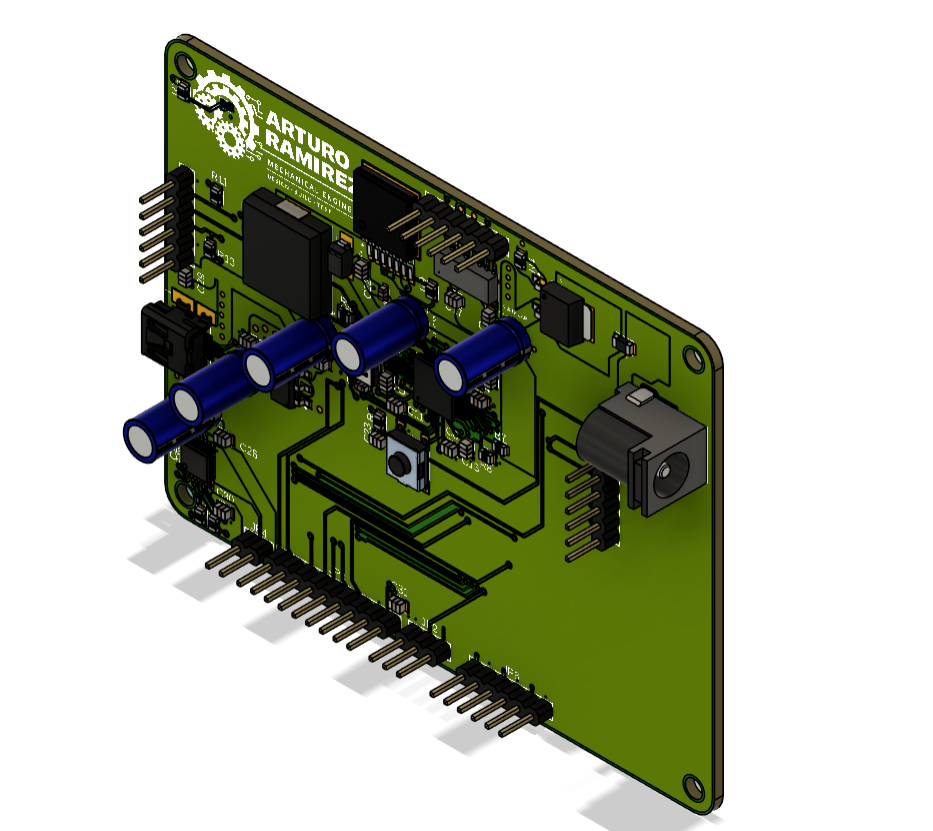
\includegraphics[
        width=3.23in,
        height=2.25in,
        keepaspectratio
    ]{pcb_render.png}
};

\node[
    anchor=north,
    align=center,
    inner sep=0pt,
    text width=3.08in,
    text=Muted,
    font=\sffamily\fontsize{6.15}{6.85}\selectfont
]
at ($(current page.north west)+(1.7in,-3.94in)$)
{Fusion 360 Electronics render of the populated controller PCB};

% Top center — fabricated PCB photograph
\node[
    anchor=north west,
    inner sep=2.6pt,
    draw=DeepGreen,
    line width=0.68pt,
    rounded corners=5pt
]
at ($(current page.north west)+(3.90in,-1.58in)$)
{
    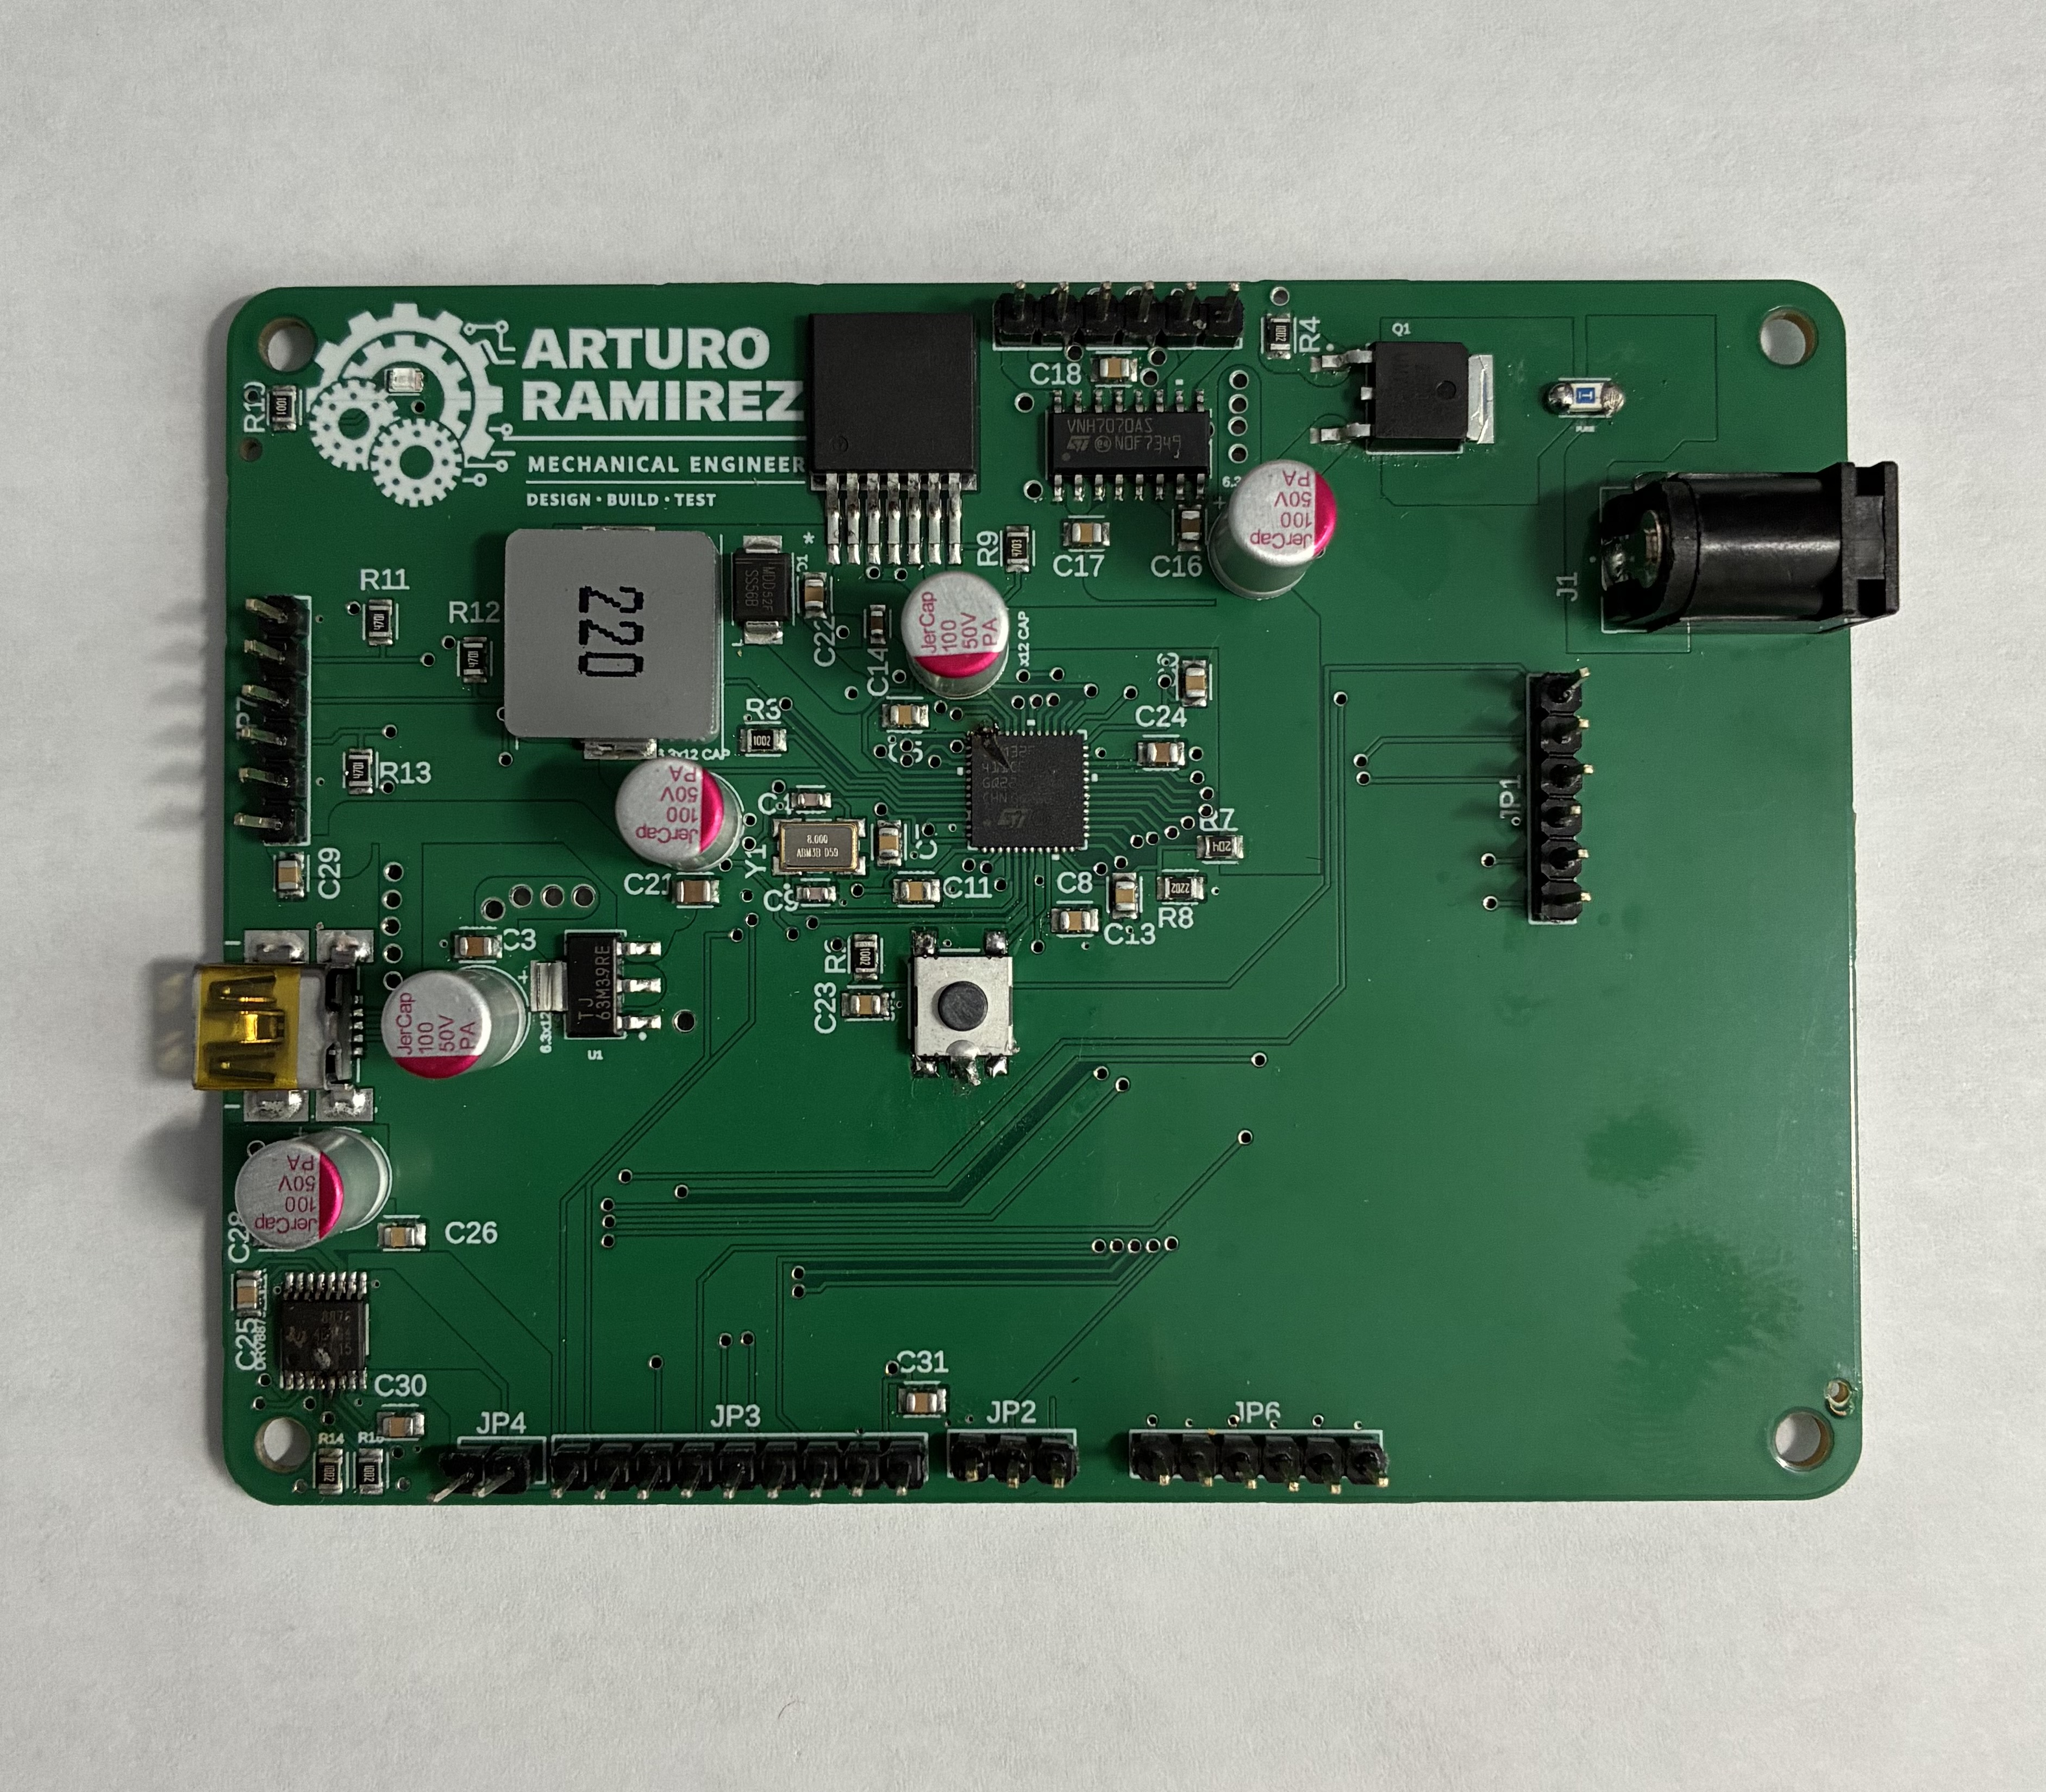
\includegraphics[
        width=3.38in,
        height=2.25in,
        keepaspectratio
    ]{complete_pcb.jpeg}
};

\node[
    anchor=north,
    align=center,
    inner sep=0pt,
    text width=3.20in,
    text=Muted,
    font=\sffamily\fontsize{6.15}{6.85}\selectfont
]
at ($(current page.north west)+(5.2in,-3.94in)$)
{Fabricated and partially populated first-generation controller PCB};

% Top right — design approach
\fill[SoftGold,rounded corners=5pt]
    ($(current page.north west)+(7.52in,-1.58in)$)
    rectangle
    ($(current page.north east)+(-0.42in,-2.71in)$);

\fill[PolyGold]
    ($(current page.north west)+(7.52in,-1.58in)$)
    rectangle
    ($(current page.north west)+(7.62in,-2.71in)$);

\node[
    anchor=north west,
    text=DeepGreen,
    font=\sffamily\bfseries\fontsize{7.8}{8.5}\selectfont
]
at ($(current page.north west)+(7.82in,-1.76in)$)
{DESIGN APPROACH};

\node[
    anchor=north west,
    align=left,
    text width=2.48in,
    text=Ink,
    font=\fontsize{5.30}{6.05}\selectfont
]
at ($(current page.north west)+(7.82in,-2.04in)$)
{
The board was developed from the system requirements outward.\\[2pt]
MCUs, drivers, regulators, connectors, passives, footprints, and
protection devices were verified against datasheets, package limits,
assembly access, and JLCPCB availability before routing.
};

% Top right — integrated features
\fill[SoftGreen,rounded corners=5pt]
    ($(current page.north west)+(7.52in,-2.91in)$)
    rectangle
    ($(current page.north east)+(-0.42in,-4.04in)$);

\draw[RuleGray,line width=0.55pt,rounded corners=5pt]
    ($(current page.north west)+(7.52in,-2.91in)$)
    rectangle
    ($(current page.north east)+(-0.42in,-4.04in)$);

\node[
    anchor=north west,
    text=DeepGreen,
    font=\sffamily\bfseries\fontsize{7.8}{8.5}\selectfont
]
at ($(current page.north west)+(7.78in,-3.09in)$)
{INTEGRATED FEATURES};

\node[
    anchor=north west,
    align=left,
    text width=2.86in,
    text=Ink,
    font=\fontsize{5.55}{6.38}\selectfont
]
at ($(current page.north west)+(7.78in,-3.37in)$)
{
STM32F411 \textbullet\ 24 V input\\
5 V buck \textbullet\ 3.3 V logic\\
Motor and actuator control\\
Dual encoder interfaces\\
SPI TFT \textbullet\ buttons \textbullet\ limit switch\\
USB \textbullet\ SWD \textbullet\ voltage sensing
};

% Routing section title
\node[
    anchor=north west,
    text=DeepGreen,
    font=\sffamily\bfseries\fontsize{8.0}{8.7}\selectfont
]
at ($(current page.north west)+(0.43in,-4.30in)$)
{ROUTING, MCU ASSIGNMENT, AND DESIGN FOR MANUFACTURING};

% Routing cards
\node[
    anchor=north west,
    inner sep=2.4pt,
    draw=RuleGray,
    line width=0.55pt,
    rounded corners=4pt
]
at ($(current page.north west)+(0.42in,-4.56in)$)
{
    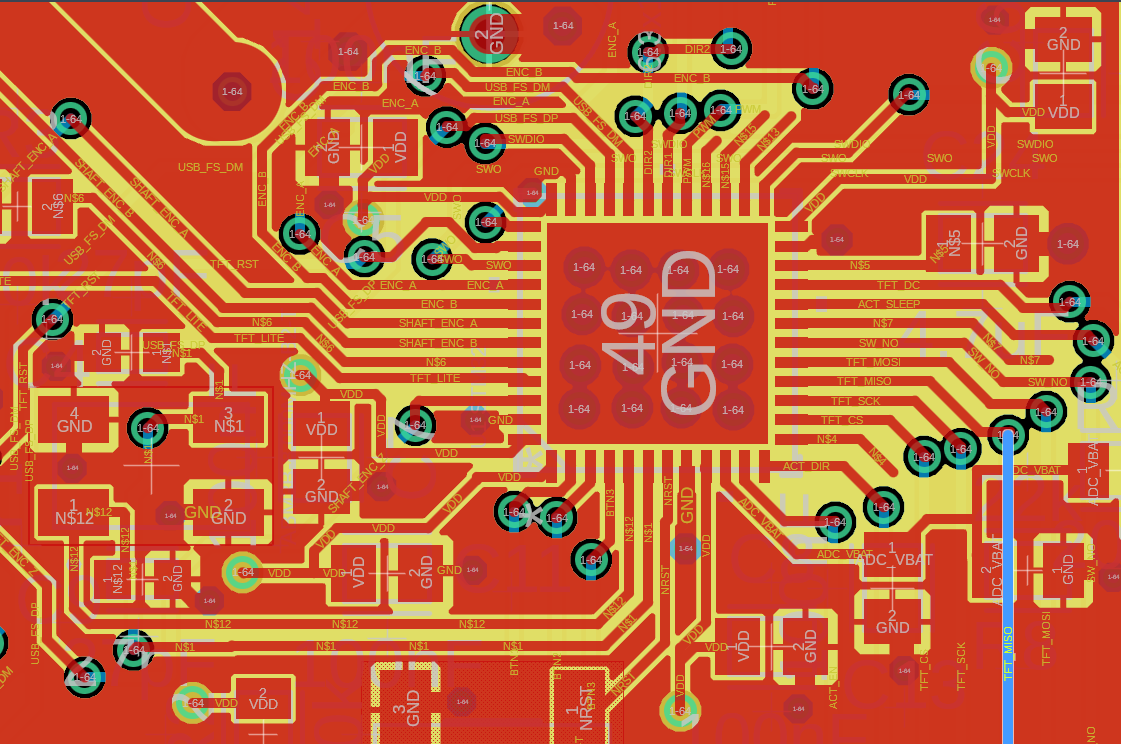
\includegraphics[
        width=3.34in,
        height=1.64in,
        keepaspectratio
    ]{Top_layer.png}
};

\node[
    anchor=north,
    align=center,
    inner sep=0pt,
    text width=3.18in,
    text=Muted,
    font=\sffamily\fontsize{6.10}{6.80}\selectfont
]
at ($(current page.north west)+(1.8in,-6.29in)$)
{Top-layer routing and component fan-out};

\node[
    anchor=north west,
    inner sep=2.4pt,
    draw=RuleGray,
    line width=0.55pt,
    rounded corners=4pt
]
at ($(current page.north west)+(3.98in,-4.56in)$)
{
    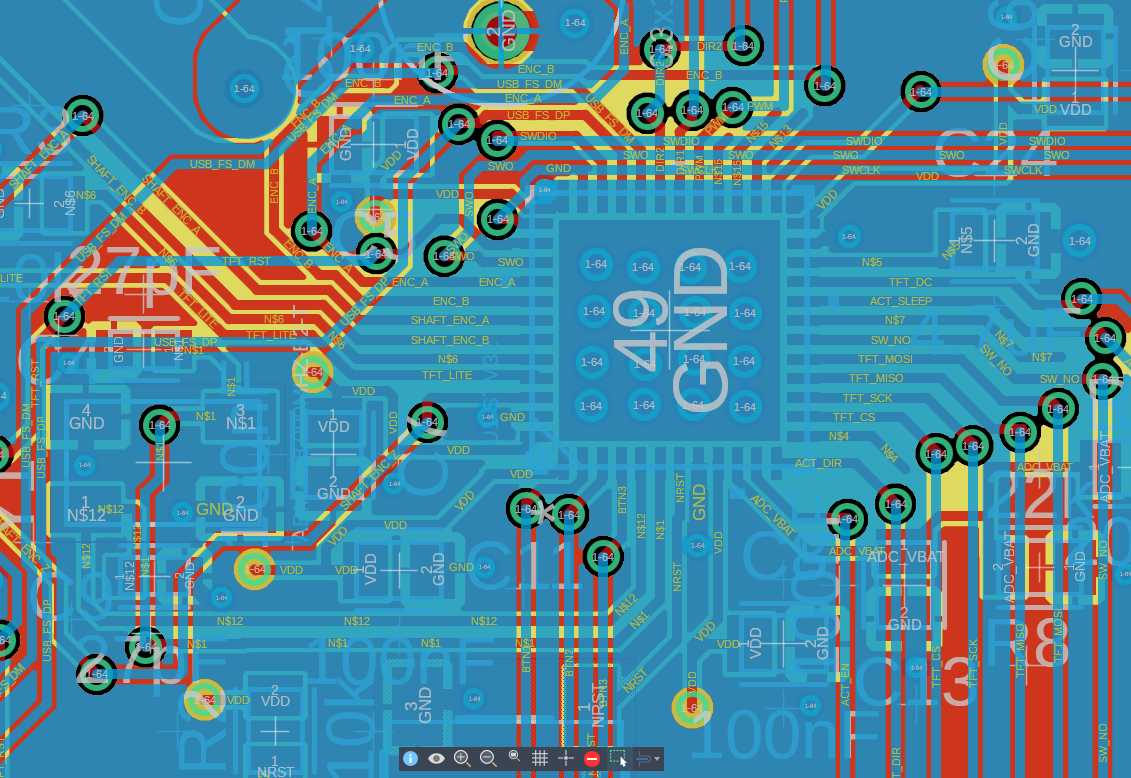
\includegraphics[
        width=3.34in,
        height=1.64in,
        keepaspectratio
    ]{bottom_layer.png}
};

\node[
    anchor=north,
    align=center,
    inner sep=0pt,
    text width=3.18in,
    text=Muted,
    font=\sffamily\fontsize{6.10}{6.80}\selectfont
]
at ($(current page.north west)+(5.3in,-6.29in)$)
{Bottom-layer routing and return-path organization};

\node[
    anchor=north west,
    inner sep=2.4pt,
    draw=RuleGray,
    line width=0.55pt,
    rounded corners=4pt
]
at ($(current page.north west)+(7.54in,-4.56in)$)
{
    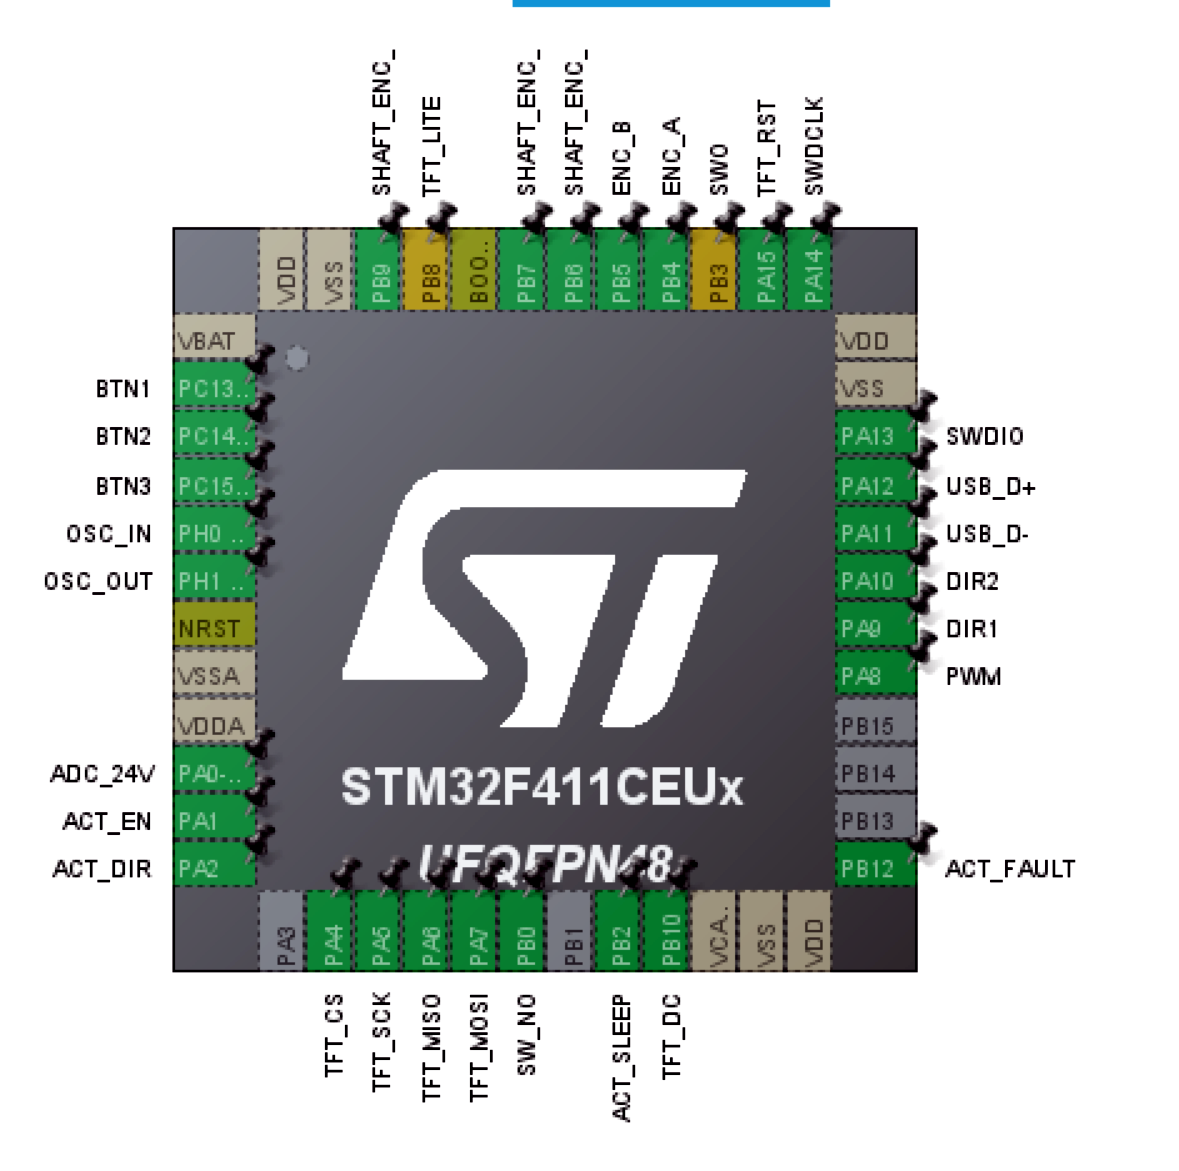
\includegraphics[
        width=3.20in,
        height=1.64in,
        keepaspectratio
    ]{stm32_pinout.png}
};

\node[
    anchor=north,
    align=center,
    inner sep=0pt,
    text width=3.04in,
    text=Muted,
    font=\sffamily\fontsize{6.10}{6.80}\selectfont
]
at ($(current page.north west)+(8.45in,-6.29in)$)
{STM32F411 GPIO and peripheral assignment};

% Bottom engineering panels
\fill[SoftGreen,rounded corners=5pt]
    ($(current page.north west)+(0.42in,-6.56in)$)
    rectangle
    ($(current page.north west)+(5.34in,-7.24in)$);

\draw[RuleGray,line width=0.55pt,rounded corners=5pt]
    ($(current page.north west)+(0.42in,-6.56in)$)
    rectangle
    ($(current page.north west)+(5.34in,-7.24in)$);

\node[
    anchor=north west,
    text=DeepGreen,
    font=\sffamily\bfseries\fontsize{7.25}{7.95}\selectfont
]
at ($(current page.north west)+(0.66in,-6.70in)$)
{POWER ARCHITECTURE};

\node[
    anchor=north west,
    align=left,
    text width=4.40in,
    text=Ink,
    font=\fontsize{6.02}{6.90}\selectfont
]
at ($(current page.north west)+(0.66in,-6.94in)$)
{
24 V motor supply \(\rightarrow\) protected input \(\rightarrow\) 5 V buck conversion
\(\rightarrow\) 3.3 V logic regulation, with local bulk and high-frequency decoupling.
};

\fill[SoftGold,rounded corners=5pt]
    ($(current page.north west)+(5.56in,-6.56in)$)
    rectangle
    ($(current page.north east)+(-0.42in,-7.24in)$);

\fill[PolyGold]
    ($(current page.north west)+(5.56in,-6.56in)$)
    rectangle
    ($(current page.north west)+(5.66in,-7.24in)$);

\node[
    anchor=north west,
    text=DeepGreen,
    font=\sffamily\bfseries\fontsize{7.25}{7.95}\selectfont
]
at ($(current page.north west)+(5.86in,-6.70in)$)
{DESIGN FOR MANUFACTURING};

\node[
    anchor=north west,
    align=left,
    text width=4.60in,
    text=Ink,
    font=\fontsize{6.00}{6.88}\selectfont
]
at ($(current page.north west)+(5.86in,-6.94in)$)
{
JLCPCB stock, assembly orientation, connector access, soldering practicality,
test access, and footprint verification directly shaped the final board.
};

% Resource links
\node[
    anchor=north,
    align=center,
    text=DeepGreen,
    font=\sffamily\bfseries\fontsize{6.75}{7.35}\selectfont
]
at ($(current page.north)+(0,-7.45in)$)
{
\href{\GearboxBOMURL}{\faFilePdf\ JLCPCB BOM}
\hspace{18pt}
\href{\GearboxPnPURL}{\faFilePdf\ PICK-AND-PLACE}
\hspace{18pt}
\href{\GearboxPinoutURL}{\faFilePdf\ PCB PINOUT LOGIC}
};

% Footer
\node[
    anchor=south west,
    text=white,
    font=\sffamily\bfseries\fontsize{7.1}{7.7}\selectfont
]
at ($(current page.south west)+(0.42in,0.17in)$)
{\faArrowLeft\ SYSTEM OVERVIEW};

\node[
    anchor=south,
    text=white,
    font=\sffamily\fontsize{7.0}{7.6}\selectfont
]
at ($(current page.south)+(0,0.17in)$)
{GEARBOX CONTROLLER \hspace{6pt} 2 / 3};

\node[
    anchor=south east,
    text=white,
    font=\sffamily\bfseries\fontsize{7.1}{7.7}\selectfont
]
at ($(current page.south east)+(-0.42in,0.17in)$)
{INTEGRATION \& TAKEAWAYS \faArrowRight};

\end{tikzpicture}

% ============================================================
% PAGE 3 — EMBEDDED INTEGRATION, LESSONS, AND FUTURE PLATFORM
% Image used on this page:
%   pcb_layer_view.png
% No Google Drive resource is repeated on this page.
% ============================================================

\clearpage
\thispagestyle{empty}
\null

\begin{tikzpicture}[remember picture,overlay]

% Background and bars
\fill[white] (current page.south west) rectangle (current page.north east);

\fill[DeepGreen]
    (current page.north west)
    rectangle
    ($(current page.north east)+(0,-0.095in)$);

\fill[PolyGold]
    ($(current page.north west)+(0,-0.095in)$)
    rectangle
    ($(current page.north east)+(0,-0.14in)$);

\fill[DeepGreen]
    (current page.south west)
    rectangle
    ($(current page.south east)+(0,0.36in)$);

\fill[PolyGold]
    ($(current page.south west)+(0,0.36in)$)
    rectangle
    ($(current page.south east)+(0,0.405in)$);

% Header
\node[
    anchor=north west,
    text=PolyGold,
    font=\sffamily\bfseries\fontsize{8.1}{8.7}\selectfont
]
at ($(current page.north west)+(0.42in,-0.39in)$)
{GEARBOX CONTROLLER \hspace{5pt}/\hspace{5pt} INTEGRATION AND ENGINEERING TAKEAWAYS};

\node[
    anchor=north west,
    text=DeepGreen,
    font=\bfseries\fontsize{22.0}{23.0}\selectfont
]
at ($(current page.north west)+(0.40in,-0.67in)$)
{A REUSABLE PLATFORM FOR EMBEDDED CONTROL};

\node[
    anchor=north west,
    text=Muted,
    font=\sffamily\fontsize{8.25}{9.0}\selectfont
]
at ($(current page.north west)+(0.42in,-1.12in)$)
{Hardware assembly, CubeMX configuration, collaborative firmware development, and next-generation expansion};

\fill[PolyGold]
    ($(current page.north west)+(0.42in,-1.36in)$)
    rectangle
    ($(current page.north west)+(8.82in,-1.315in)$);

% Large PCB routing image — only use of this image
\node[
    anchor=north west,
    inner sep=2.6pt,
    draw=DeepGreen,
    line width=0.68pt,
    rounded corners=5pt
]
at ($(current page.north west)+(0.42in,-1.58in)$)
{
    \includegraphics[
        width=5.20in,
        height=3.15in,
        keepaspectratio
    ]{pcb_layer_view.png}
};

\node[
    anchor=north,
    align=center,
    inner sep=0pt,
    text width=4.98in,
    text=Muted,
    font=\sffamily\fontsize{6.30}{7.00}\selectfont
]
at ($(current page.north west)+(3.02in,-4.85in)$)
{Dense MCU breakout, encoder routing, SWD, USB, TFT, actuator, and sensing interfaces};

% Top right — hardware and firmware integration
% Left edge aligned with the Future Learning Platform panel below.
\fill[SoftGold,rounded corners=5pt]
    ($(current page.north west)+(5.56in,-1.58in)$)
    rectangle
    ($(current page.north east)+(-0.42in,-4.92in)$);

\fill[PolyGold]
    ($(current page.north west)+(5.56in,-1.58in)$)
    rectangle
    ($(current page.north west)+(5.66in,-4.92in)$);

\node[
    anchor=north west,
    text=DeepGreen,
    font=\sffamily\bfseries\fontsize{8.0}{8.7}\selectfont
]
at ($(current page.north west)+(5.86in,-1.77in)$)
{HARDWARE AND FIRMWARE INTEGRATION};

\node[
    anchor=north west,
    align=left,
    text width=4.54in,
    text=Ink,
    font=\fontsize{6.65}{7.78}\selectfont
]
at ($(current page.north west)+(5.86in,-2.07in)$)
{
After fabrication, I soldered the selected components and integrated the
PCB into the larger system architecture. My partner and I jointly configured
the STM32 in CubeMX to establish clocking, GPIO, timers, encoder inputs,
SPI communication, USB, and debug access.\\[5pt]

We developed the firmware around collaborative multitasking in C/C++ so
that motor control, display updates, user commands, actuator behavior, and
safety logic could operate as one cohesive controller rather than as isolated
demonstrations.\\[5pt]

This first revision served as a functional learning platform while exposing
practical improvements for protection, test access, connector planning,
packaging, and future instrumentation.
};

% Bottom left — engineering takeaways
\fill[SoftGreen,rounded corners=5pt]
    ($(current page.north west)+(0.42in,-5.18in)$)
    rectangle
    ($(current page.north west)+(5.34in,-7.30in)$);

\draw[RuleGray,line width=0.55pt,rounded corners=5pt]
    ($(current page.north west)+(0.42in,-5.18in)$)
    rectangle
    ($(current page.north west)+(5.34in,-7.30in)$);

\node[
    anchor=north west,
    text=DeepGreen,
    font=\sffamily\bfseries\fontsize{7.8}{8.5}\selectfont
]
at ($(current page.north west)+(0.68in,-5.36in)$)
{ENGINEERING TAKEAWAYS};

\node[
    anchor=north west,
    align=left,
    text width=4.42in,
    text=Ink,
    font=\fontsize{6.25}{7.25}\selectfont
]
at ($(current page.north west)+(0.68in,-5.65in)$)
{
\textbf{Architecture first.}
Defining interfaces before routing reduced late-stage changes and simplified integration.\\[4pt]

\textbf{Datasheets are the design language.}
Selection required verifying voltage, current, package, thermal, and control requirements rather than relying on names alone.\\[4pt]

\textbf{Manufacturability shapes electronics.}
Stock, assembly, access, solderability, and testability directly influenced the final circuit.\\[4pt]

\textbf{First revisions are learning tools.}
Bring-up revealed improvements for protection, debug access, and packaging.
};

% Bottom right — future platform
\fill[SoftGold,rounded corners=5pt]
    ($(current page.north west)+(5.56in,-5.18in)$)
    rectangle
    ($(current page.north east)+(-0.42in,-7.30in)$);

\fill[PolyGold]
    ($(current page.north west)+(5.56in,-5.18in)$)
    rectangle
    ($(current page.north west)+(5.66in,-7.30in)$);

\node[
    anchor=north west,
    text=DeepGreen,
    font=\sffamily\bfseries\fontsize{7.8}{8.5}\selectfont
]
at ($(current page.north west)+(5.86in,-5.36in)$)
{FUTURE LEARNING PLATFORM};

\node[
    anchor=north west,
    align=left,
    text width=4.58in,
    text=Ink,
    font=\fontsize{6.25}{7.25}\selectfont
]
at ($(current page.north west)+(5.86in,-5.65in)$)
{
The controller was intentionally conceived as more than a single-purpose
gearbox driver. Future revisions can add torque sensing, motor-current
measurement, temperature monitoring, improved output-speed sensing,
and additional analog or digital sensors.\\[5pt]

Those additions would support system identification, efficiency studies,
closed-loop speed control, comparison between predicted and measured
gear ratios, and the development of kinetic as well as kinematic models.
The existing PCB, enclosure, display, and modular mechanical platform
provide the foundation for those experiments.
};

% Footer
\node[
    anchor=south west,
    text=white,
    font=\sffamily\bfseries\fontsize{7.1}{7.7}\selectfont
]
at ($(current page.south west)+(0.42in,0.17in)$)
{\faArrowLeft\ PCB ARCHITECTURE};

\node[
    anchor=south,
    text=white,
    font=\sffamily\fontsize{7.0}{7.6}\selectfont
]
at ($(current page.south)+(0,0.17in)$)
{GEARBOX CONTROLLER \hspace{6pt} 3 / 3};

\node[
    anchor=south east,
    text=white,
    font=\sffamily\bfseries\fontsize{7.1}{7.7}\selectfont
]
at ($(current page.south east)+(-0.42in,0.17in)$)
{NEXT PROJECT \faArrowRight};

\end{tikzpicture}


% ============================================================
% ROMI AUTONOMOUS DIFFERENTIAL-DRIVE ROBOT
% FIVE-PAGE PORTFOLIO CASE STUDY
% 02 Mechatronics / Project 07
%
% IMPORTANT
% ----------
% 1. This file is intended to be included from the main portfolio:
%       \input{romi}
%    It must NOT contain \documentclass, \begin{document}, or \end{document}.
%
% 2. The main preamble should already define:
%       DeepGreen, PolyGold, SoftGold, SoftGreen,
%       RuleGray, Muted, Ink, Panel
%    and load:
%       tikz, graphicx, hyperref, fontawesome5, amsmath, amssymb
%
% 3. Upload the following image files to Overleaf using these exact
%    base filenames. Extensions may be .png, .jpg, or .jpeg; LaTeX will
%    resolve them automatically when only the base filename is supplied.
%
%       Romi Hero Image
%       Romi Pluggedin
%       Romi Side View
%       Romi Top View
%       Real Time Software Diagram
%       Chassis Dynamics
%       Dynamics
%       Romi Total Dynamics
%       Wheel Encoder Rotation
%       effort based position
%       effort based velocity
%       gain calibration
%       nested control loop
%       Track Course
%
%    Each image is used only once in this script.
%
% 4. The instructor's timer auto-reload visualization is intentionally
%    excluded because the page prioritizes team-created engineering artifacts.
%
% 5. The notebook HTML button should only be restored after the file has
%    been uploaded to a public HTTPS address. Local file:/// and run: links
%    are intentionally excluded because they break for other viewers.
%
% 6. Resource links are each used once across the five pages.
% ============================================================

% ------------------------------------------------------------
% PROJECT RESOURCE URLS
% ------------------------------------------------------------

\providecommand{\RomiGitHubURL}
{https://github.com/shwanpla/ME-405-Term-Project}

\providecommand{\RomiDocumentationURL}
{https://me-405-term-project.readthedocs.io/en/latest/overview.html}

\providecommand{\RomiTrackYouTubeURL}
{https://youtu.be/gsIIfVX_UOE?si=vdGteQbXHBkoHcBp}

\providecommand{\RomiLineYouTubeURL}
{https://youtu.be/3hr3dCyPbDM?si=kXSeATZV6t0dCAKc}

\providecommand{\RomiDataCaptureURL}
{https://drive.google.com/file/d/1NIpuxDYtf03tbfd8yQCP5n-v_P9-T6j7/view?usp=drive_link}

% Replace this placeholder with the HTML-export link supplied for the project.
% IMPORTANT: A file:///D:/... path is private to one computer and cannot
% be opened by employers. Upload HW0x04_ARTURO_RAMIREZ.html to a public host
% such as GitHub Pages, Google Drive with public access, or a personal website,
% then replace the URL below with that absolute https:// address.
%
% Example after enabling GitHub Pages:
% https://YOUR-USERNAME.github.io/YOUR-REPOSITORY/HW0x04_ARTURO_RAMIREZ.html
%
% Until a public URL is supplied, the notebook button is intentionally omitted
% from the resource row so the portfolio contains no broken link.
\providecommand{\RomiNotebookHTMLURL}
{https://art675.github.io/Romi-Dynamics-Study/}

% ============================================================
% PAGE 1 — SYSTEM OVERVIEW AND PHYSICAL INTEGRATION
% ============================================================

\clearpage
\thispagestyle{empty}
\hypertarget{romi}{}
\null

\begin{tikzpicture}[remember picture,overlay]

% Background and page bars
\fill[white] (current page.south west) rectangle (current page.north east);

\fill[DeepGreen]
    (current page.north west)
    rectangle
    ($(current page.north east)+(0,-0.095in)$);

\fill[PolyGold]
    ($(current page.north west)+(0,-0.095in)$)
    rectangle
    ($(current page.north east)+(0,-0.14in)$);

\fill[DeepGreen]
    (current page.south west)
    rectangle
    ($(current page.south east)+(0,0.36in)$);

\fill[PolyGold]
    ($(current page.south west)+(0,0.36in)$)
    rectangle
    ($(current page.south east)+(0,0.405in)$);

% Header
\node[
    anchor=north west,
    text=PolyGold,
    font=\sffamily\bfseries\fontsize{8.1}{8.7}\selectfont
]
at ($(current page.north west)+(0.42in,-0.39in)$)
{02 MECHATRONICS \hspace{5pt}/\hspace{5pt} PROJECT 07};

\node[
    anchor=north west,
    text=DeepGreen,
    font=\bfseries\fontsize{22.4}{23.4}\selectfont
]
at ($(current page.north west)+(0.40in,-0.67in)$)
{ROMI AUTONOMOUS DIFFERENTIAL-DRIVE ROBOT};

\node[
    anchor=north west,
    text=Muted,
    font=\sffamily\fontsize{8.25}{9.0}\selectfont
]
at ($(current page.north west)+(0.42in,-1.12in)$)
{Cal Poly Mechatronics Laboratory
\hspace{7pt}\textbullet\hspace{7pt}
Three-Person Team
\hspace{7pt}\textbullet\hspace{7pt}
Fall 2025
\hspace{7pt}\textbullet\hspace{7pt}
San Luis Obispo, California};

\fill[PolyGold]
    ($(current page.north west)+(0.42in,-1.36in)$)
    rectangle
    ($(current page.north west)+(8.90in,-1.315in)$);

% Hero image
\node[
    anchor=north west,
    inner sep=2.7pt,
    draw=DeepGreen,
    line width=0.70pt,
    rounded corners=6pt
]
at ($(current page.north west)+(0.42in,-1.58in)$)
{
    \includegraphics[
        width=5.18in,
        height=3.26in,
        keepaspectratio
    ]{\detokenize{Romi Hero Image}}
};

\node[
    anchor=north,
    align=center,
    inner sep=0pt,
    text width=4.95in,
    text=Muted,
    font=\sffamily\fontsize{6.30}{7.00}\selectfont
]
at ($(current page.north west)+(3.01in,-4.94in)$)
{Final Romi autonomous robot.};

% Project overview
% Extended farther left while preserving the original 0.10 in accent strip.
\fill[SoftGold,rounded corners=5pt]
    ($(current page.north west)+(4.43in,-1.58in)$)
    rectangle
    ($(current page.north east)+(-0.42in,-4.98in)$);

\fill[PolyGold]
    ($(current page.north west)+(4.43in,-1.58in)$)
    rectangle
    ($(current page.north west)+(4.53in,-4.98in)$);

\node[
    anchor=north west,
    text=DeepGreen,
    font=\sffamily\bfseries\fontsize{8.0}{8.7}\selectfont
]
at ($(current page.north west)+(4.73in,-1.76in)$)
{PROJECT OVERVIEW};

\node[
    anchor=north west,
    align=left,
    text width=5.73in,
    text=Ink,
    font=\fontsize{6.45}{7.50}\selectfont
]
at ($(current page.north west)+(4.73in,-2.05in)$)
{
Our three-person team built a fully integrated autonomous differential-drive
robot for a course-specific navigation challenge. The system combined an
STM32 Nucleo running MicroPython, wheel encoders, a QTR reflectance array,
a BNO055 IMU, bumper sensing, Bluetooth/serial telemetry, and closed-loop
motor control.\\[4pt]

The software architecture separated hardware drivers, periodic sensing,
state estimation, velocity control, data processing, communications, and
navigation into cooperative generator-based tasks. Shared variables and
queues provided explicit interfaces between subsystems while a priority-based
scheduler maintained deterministic update periods.\\[4pt]

Programming, dynamic analysis, controller tuning, testing, and integration
were shared across the team. The project emphasized collaborative code
development rather than isolated subsystem ownership.
};

\node[
    anchor=south west,
    text=PolyGold,
    font=\sffamily\bfseries\fontsize{6.25}{6.95}\selectfont
]
at ($(current page.north west)+(4.73in,-4.82in)$)
{MICROPYTHON \hspace{6pt}\textbullet\hspace{6pt}
STM32 \hspace{6pt}\textbullet\hspace{6pt}
COOPERATIVE MULTITASKING \hspace{6pt}\textbullet\hspace{6pt}
CLOSED-LOOP CONTROL};

% Supporting hardware images
\node[
    anchor=north west,
    text=DeepGreen,
    font=\sffamily\bfseries\fontsize{8.0}{8.7}\selectfont
]
at ($(current page.north west)+(0.43in,-5.22in)$)
{HARDWARE BRING-UP AND SENSOR INTEGRATION};

% Equal-width light-green image cards
\fill[SoftGreen!46,rounded corners=5pt]
    ($(current page.north west)+(0.42in,-5.48in)$)
    rectangle
    ($(current page.north west)+(3.63in,-7.18in)$);

\draw[RuleGray,line width=0.55pt,rounded corners=5pt]
    ($(current page.north west)+(0.42in,-5.48in)$)
    rectangle
    ($(current page.north west)+(3.63in,-7.18in)$);

\fill[SoftGreen!46,rounded corners=5pt]
    ($(current page.north west)+(4.05in,-5.48in)$)
    rectangle
    ($(current page.north west)+(7.26in,-7.18in)$);

\draw[RuleGray,line width=0.55pt,rounded corners=5pt]
    ($(current page.north west)+(4.05in,-5.48in)$)
    rectangle
    ($(current page.north west)+(7.26in,-7.18in)$);

\fill[SoftGreen!46,rounded corners=5pt]
    ($(current page.north west)+(7.46in,-5.48in)$)
    rectangle
    ($(current page.north west)+(10.67in,-7.18in)$);

\draw[RuleGray,line width=0.55pt,rounded corners=5pt]
    ($(current page.north west)+(7.46in,-5.48in)$)
    rectangle
    ($(current page.north west)+(10.67in,-7.18in)$);

% Card 1 — firmware flashing
\node[
    anchor=north,
    inner sep=2.2pt,
    draw=RuleGray,
    line width=0.50pt,
    rounded corners=3pt,
    fill=white
]
at ($(current page.north west)+(2.025in,-5.61in)$)
{
    \includegraphics[
        width=2.82in,
        height=1.17in,
        keepaspectratio
    ]{\detokenize{Romi Pluggedin}}
};

\node[
    anchor=north,
    align=center,
    text width=2.78in,
    text=Muted,
    font=\sffamily\fontsize{6.25}{6.85}\selectfont
]
at ($(current page.north west)+(2.025in,-6.91in)$)
{Firmware flashing};

% Card 2 — side view
\node[
    anchor=north,
    inner sep=2.2pt,
    draw=RuleGray,
    line width=0.50pt,
    rounded corners=3pt,
    fill=white
]
at ($(current page.north west)+(5.655in,-5.61in)$)
{
    \includegraphics[
        width=2.82in,
        height=1.17in,
        keepaspectratio
    ]{\detokenize{Romi Side View}}
};

\node[
    anchor=north,
    align=center,
    text width=2.78in,
    text=Muted,
    font=\sffamily\fontsize{6.25}{6.85}\selectfont
]
at ($(current page.north west)+(5.655in,-6.91in)$)
{Side view};

% Card 3 — top view
\node[
    anchor=north,
    inner sep=2.2pt,
    draw=RuleGray,
    line width=0.50pt,
    rounded corners=3pt,
    fill=white
]
at ($(current page.north west)+(9.065in,-5.61in)$)
{
    \includegraphics[
        width=2.82in,
        height=1.17in,
        keepaspectratio
    ]{\detokenize{Romi Top View}}
};

\node[
    anchor=north,
    align=center,
    text width=2.78in,
    text=Muted,
    font=\sffamily\fontsize{6.25}{6.85}\selectfont
]
at ($(current page.north west)+(9.065in,-6.91in)$)
{Top view};

% Footer
\node[
    anchor=south west,
    text=white,
    font=\sffamily\bfseries\fontsize{7.1}{7.7}\selectfont
]
at ($(current page.south west)+(0.42in,0.17in)$)
{\hyperlink{gearboxpcb}{\faArrowLeft\ GEARBOX CONTROLLER}};

\node[
    anchor=south,
    text=white,
    font=\sffamily\fontsize{7.0}{7.6}\selectfont
]
at ($(current page.south)+(0,0.17in)$)
{ROMI AUTONOMOUS ROBOT \hspace{6pt} 1 / 5};

\node[
    anchor=south east,
    text=white,
    font=\sffamily\bfseries\fontsize{7.1}{7.7}\selectfont
]
at ($(current page.south east)+(-0.42in,0.17in)$)
{SOFTWARE ARCHITECTURE \faArrowRight};

\end{tikzpicture}

% ============================================================
% PAGE 2 — REAL-TIME SOFTWARE ARCHITECTURE
% ============================================================

\clearpage
\thispagestyle{empty}
\null

\begin{tikzpicture}[remember picture,overlay]

\fill[white] (current page.south west) rectangle (current page.north east);
\fill[DeepGreen] (current page.north west) rectangle ($(current page.north east)+(0,-0.095in)$);
\fill[PolyGold] ($(current page.north west)+(0,-0.095in)$) rectangle ($(current page.north east)+(0,-0.14in)$);
\fill[DeepGreen] (current page.south west) rectangle ($(current page.south east)+(0,0.36in)$);
\fill[PolyGold] ($(current page.south west)+(0,0.36in)$) rectangle ($(current page.south east)+(0,0.405in)$);

\node[
    anchor=north west,
    text=PolyGold,
    font=\sffamily\bfseries\fontsize{8.1}{8.7}\selectfont
]
at ($(current page.north west)+(0.42in,-0.39in)$)
{ROMI AUTONOMOUS ROBOT \hspace{5pt}/\hspace{5pt} REAL-TIME SOFTWARE};

\node[
    anchor=north west,
    text=DeepGreen,
    font=\bfseries\fontsize{22.0}{23.0}\selectfont
]
at ($(current page.north west)+(0.40in,-0.67in)$)
{COOPERATIVE TASK ARCHITECTURE AND DATA FLOW};

\node[
    anchor=north west,
    text=Muted,
    font=\sffamily\fontsize{8.25}{9.0}\selectfont
]
at ($(current page.north west)+(0.42in,-1.12in)$)
{Generator-based tasks, shared variables, queues, priorities, periods, and finite-state navigation};

\fill[PolyGold]
    ($(current page.north west)+(0.42in,-1.36in)$)
    rectangle
    ($(current page.north west)+(8.72in,-1.315in)$);

% Main architecture image
\node[
    anchor=north west,
    inner sep=2.8pt,
    draw=DeepGreen,
    line width=0.68pt,
    rounded corners=5pt
]
at ($(current page.north west)+(0.42in,-1.58in)$)
{
    \includegraphics[
        width=6.74in,
        height=5.55in,
        keepaspectratio
    ]{\detokenize{Real Time Software Diagram}}
};

\node[
    anchor=north,
    align=center,
    text width=6.45in,
    text=Muted,
    font=\sffamily\fontsize{6.25}{6.95}\selectfont
]
at ($(current page.north west)+(3.79in,-7.25in)$)
{Team-developed real-time task diagram showing priorities, periods, shared data, commands, and telemetry paths};

% Architecture explanation
\fill[SoftGold,rounded corners=5pt]
    ($(current page.north west)+(6.62in,-1.58in)$)
    rectangle
    ($(current page.north east)+(-0.42in,-3.58in)$);

\fill[PolyGold]
    ($(current page.north west)+(6.62in,-1.58in)$)
    rectangle
    ($(current page.north west)+(6.72in,-3.58in)$);

\node[
    anchor=north west,
    text=DeepGreen,
    font=\sffamily\bfseries\fontsize{7.8}{8.5}\selectfont
]
at ($(current page.north west)+(7.00in,-1.76in)$)
{WHY THE ARCHITECTURE MATTERED};

\node[
    anchor=north west,
    align=left,
    text width=3.28in,
    text=Ink,
    font=\fontsize{5.52}{6.34}\selectfont
]
at ($(current page.north west)+(6.96in,-2.05in)$)
{
Each subsystem ran as a periodic generator task rather than as one
monolithic loop. This kept sensing, estimation, control, navigation,
data logging, and communications independently testable while preserving
deterministic update timing.\\[3.5pt]

Queues carried ordered data streams; shared variables exposed the latest
state or command; object interfaces encapsulated hardware drivers.
};

% Software stack
\fill[SoftGreen,rounded corners=5pt]
    ($(current page.north west)+(6.62in,-3.82in)$)
    rectangle
    ($(current page.north east)+(-0.42in,-5.53in)$);

\draw[RuleGray,line width=0.55pt,rounded corners=5pt]
    ($(current page.north west)+(6.62in,-3.82in)$)
    rectangle
    ($(current page.north east)+(-0.42in,-5.53in)$);

\node[
    anchor=north west,
    text=DeepGreen,
    font=\sffamily\bfseries\fontsize{7.8}{8.5}\selectfont
]
at ($(current page.north west)+(6.88in,-4.00in)$)
{SOFTWARE STACK};

\node[
    anchor=north west,
    align=left,
    text width=3.56in,
    text=Ink,
    font=\fontsize{5.68}{6.50}\selectfont
]
at ($(current page.north west)+(6.88in,-4.28in)$)
{
\textbf{High level:} main scheduler, navigation FSM, user commands\\[3pt]
\textbf{Middle level:} control, observer, data processing, serial tasks\\[3pt]
\textbf{Low level:} motors, encoders, ADC, I\textsuperscript{2}C IMU, bump and line sensors\\[3pt]
\textbf{Interfaces:} Bluetooth/USB telemetry, reusable classes, explicit task boundaries
};

% Timing panel
\fill[SoftGold,rounded corners=5pt]
    ($(current page.north west)+(6.62in,-5.77in)$)
    rectangle
    ($(current page.north east)+(-0.42in,-7.12in)$);

\fill[PolyGold]
    ($(current page.north west)+(6.62in,-5.77in)$)
    rectangle
    ($(current page.north west)+(6.72in,-7.12in)$);

\node[
    anchor=north west,
    text=DeepGreen,
    font=\sffamily\bfseries\fontsize{7.8}{8.5}\selectfont
]
at ($(current page.north west)+(6.92in,-5.95in)$)
{IMPLEMENTATION DISCIPLINE};

\node[
    anchor=north west,
    align=left,
    text width=3.52in,
    text=Ink,
    font=\fontsize{5.72}{6.54}\selectfont
]
at ($(current page.north west)+(6.92in,-6.23in)$)
{
Tasks were assigned explicit priorities and periods according to control
bandwidth and I/O demands. Incremental integration, serial telemetry, and
repeatable trials made timing errors, stale data, state-transition faults,
and gain interactions visible early.
};

% Resource links
\node[
    anchor=north,
    align=center,
    text=DeepGreen,
    font=\sffamily\bfseries\fontsize{6.75}{7.35}\selectfont
]
at ($(current page.north)+(0,-7.48in)$)
{
\href{\RomiGitHubURL}{\faGithub\ SOURCE CODE}
\hspace{22pt}
\href{\RomiDocumentationURL}{\faBook\ DOCUMENTATION}
};

% Footer
\node[
    anchor=south west,
    text=white,
    font=\sffamily\bfseries\fontsize{7.1}{7.7}\selectfont
]
at ($(current page.south west)+(0.42in,0.17in)$)
{\faArrowLeft\ SYSTEM OVERVIEW};

\node[
    anchor=south,
    text=white,
    font=\sffamily\fontsize{7.0}{7.6}\selectfont
]
at ($(current page.south)+(0,0.17in)$)
{ROMI AUTONOMOUS ROBOT \hspace{6pt} 2 / 5};

\node[
    anchor=south east,
    text=white,
    font=\sffamily\bfseries\fontsize{7.1}{7.7}\selectfont
]
at ($(current page.south east)+(-0.42in,0.17in)$)
{DYNAMIC MODELING \faArrowRight};

\end{tikzpicture}

% ============================================================
% PAGE 3 — DIFFERENTIAL-DRIVE DYNAMICS AND STATE MODELING
% ============================================================

\clearpage
\thispagestyle{empty}
\null

\begin{tikzpicture}[remember picture,overlay]

\fill[white] (current page.south west) rectangle (current page.north east);
\fill[DeepGreen] (current page.north west) rectangle ($(current page.north east)+(0,-0.095in)$);
\fill[PolyGold] ($(current page.north west)+(0,-0.095in)$) rectangle ($(current page.north east)+(0,-0.14in)$);
\fill[DeepGreen] (current page.south west) rectangle ($(current page.south east)+(0,0.36in)$);
\fill[PolyGold] ($(current page.south west)+(0,0.36in)$) rectangle ($(current page.south east)+(0,0.405in)$);

\node[
    anchor=north west,
    text=PolyGold,
    font=\sffamily\bfseries\fontsize{8.1}{8.7}\selectfont
]
at ($(current page.north west)+(0.42in,-0.39in)$)
{ROMI AUTONOMOUS ROBOT \hspace{5pt}/\hspace{5pt} DYNAMIC MODELING};

\node[
    anchor=north west,
    text=DeepGreen,
    font=\bfseries\fontsize{21.6}{22.6}\selectfont
]
at ($(current page.north west)+(0.40in,-0.67in)$)
{FROM WHEEL MOTION TO NONLINEAR ROBOT DYNAMICS};

\node[
    anchor=north west,
    text=Muted,
    font=\sffamily\fontsize{8.15}{8.9}\selectfont
]
at ($(current page.north west)+(0.42in,-1.12in)$)
{Differential-drive kinematics, state selection, first-order motor dynamics, and observer-oriented modeling};

\fill[PolyGold]
    ($(current page.north west)+(0.42in,-1.36in)$)
    rectangle
    ($(current page.north west)+(9.25in,-1.315in)$);

% Kinematics images
\node[
    anchor=north west,
    inner sep=2.4pt,
    draw=RuleGray,
    line width=0.55pt,
    rounded corners=4pt
]
at ($(current page.north west)+(0.42in,-1.58in)$)
{
    \includegraphics[
        width=3.78in,
        height=2.30in,
        keepaspectratio
    ]{\detokenize{Chassis Dynamics}}
};

\node[
    anchor=north west,
    inner sep=2.4pt,
    draw=RuleGray,
    line width=0.55pt,
    rounded corners=4pt
]
at ($(current page.north west)+(4.42in,-1.58in)$)
{
    \includegraphics[
        width=3.78in,
        height=2.30in,
        keepaspectratio
    ]{\detokenize{Dynamics}}
};

\node[
    anchor=north west,
    inner sep=2.4pt,
    draw=RuleGray,
    line width=0.55pt,
    rounded corners=4pt
]
at ($(current page.north west)+(8.43in,-1.58in)$)
{
    \includegraphics[
        width=3.32in,
        height=2.08in,
        keepaspectratio
    ]{\detokenize{Romi Total Dynamics}}
};

\node[
    anchor=north,
    align=center,
    text width=3.55in,
    text=Muted,
    font=\sffamily\fontsize{6.0}{6.7}\selectfont
]
at ($(current page.north west)+(2.31in,-3.81in)$)
{Wheel-speed difference determines yaw rate};

\node[
    anchor=north,
    align=center,
    text width=3.55in,
    text=Muted,
    font=\sffamily\fontsize{6.0}{6.7}\selectfont
]
at ($(current page.north west)+(6.31in,-3.81in)$)
{Wheel-speed average determines forward speed};

\node[
    anchor=north,
    align=center,
    text width=3.10in,
    text=Muted,
    font=\sffamily\fontsize{6.0}{6.7}\selectfont
]
at ($(current page.north west)+(9.7in,-3.81in)$)
{Body velocity mapped into the global frame};

% State vector approach image
% Enlarged while preserving top-edge alignment with the nonlinear model panel.
\node[
    anchor=north west,
    inner sep=2.5pt,
    draw=DeepGreen,
    line width=0.65pt,
    rounded corners=5pt
]
at ($(current page.north west)+(0.42in,-4.03in)$)
{
    \includegraphics[
        width=3.58in,
        height=2.10in,
        keepaspectratio
    ]{\detokenize{Wheel Encoder Rotation}}
};

\node[
    anchor=north,
    align=center,
    text width=3.10in,
    text=Muted,
    font=\sffamily\fontsize{6.0}{6.7}\selectfont
]
at ($(current page.north west)+(1.98in,-6.34in)$)
{Manual wheel rotation used to validate encoder position tracking};

% Nonlinear model panel
\fill[SoftGold,rounded corners=5pt]
    ($(current page.north west)+(3.70in,-4.03in)$)
    rectangle
    ($(current page.north east)+(-0.42in,-6.30in)$);

\fill[PolyGold]
    ($(current page.north west)+(3.70in,-4.03in)$)
    rectangle
    ($(current page.north west)+(3.80in,-6.30in)$);

\node[
    anchor=north west,
    text=DeepGreen,
    font=\sffamily\bfseries\fontsize{7.8}{8.5}\selectfont
]
at ($(current page.north west)+(4.00in,-4.21in)$)
{NONLINEAR STATE MODEL};

% State and input column vectors
% array is used inside scalable brackets so the entries remain vertically stacked.
\node[
    anchor=north west,
    inner sep=0pt,
    text=Ink,
    font=\fontsize{6.85}{8.00}\selectfont
]
at ($(current page.north west)+(4.00in,-4.48in)$)
{%
$\displaystyle
\mathbf{x}
=
\left[
\begin{array}{c}
X\\
Y\\
\psi\\
s\\
\Omega_L\\
\Omega_R
\end{array}
\right]
$%
};

\node[
    anchor=north west,
    inner sep=0pt,
    text=Ink,
    font=\fontsize{6.85}{8.00}\selectfont
]
at ($(current page.north west)+(4.88in,-4.48in)$)
{%
$\displaystyle
\mathbf{u}
=
\left[
\begin{array}{c}
u_L\\
u_R
\end{array}
\right]
$%
};

% Standard state-space organizational form
\node[
    anchor=north west,
    inner sep=0pt,
    text=Ink,
    font=\fontsize{6.80}{7.85}\selectfont
]
at ($(current page.north west)+(4.00in,-5.30in)$)
{%
$\displaystyle
\dot{\mathbf{x}}
=
A\mathbf{x}
+
B\mathbf{u}
$%
};

% Explanation of the modeling distinction
\node[
    anchor=north west,
    align=left,
    text width=4.58in,
    text=Ink,
    font=\fontsize{5.55}{6.34}\selectfont
]
at ($(current page.north west)+(5.72in,-4.48in)$)
{
The state contains global position, robot heading, traveled distance, and
left- and right-wheel angular velocities; the inputs are commanded motor
voltages. The standard state-space organization is shown at left. However,
because the kinematic equations contain $\sin\psi$ and $\cos\psi$, the
complete robot cannot be represented by constant $A$ and $B$ matrices over
its full operating range. The project therefore used the nonlinear governing
equations for modeling while applying linear state-space methods where
appropriate for controller and observer design.
};

% Governing nonlinear equations
\node[
    anchor=north,
    align=center,
    text=Ink,
    font=\fontsize{7.35}{8.72}\selectfont
]
at ($(current page.north west)+(7.22in,-5.29in)$)
{
$\displaystyle
\dot X=\frac{r}{2}(\Omega_R+\Omega_L)\cos\psi
\qquad
\dot Y=\frac{r}{2}(\Omega_R+\Omega_L)\sin\psi
$
};

\node[
    anchor=north,
    align=center,
    text=Ink,
    font=\fontsize{7.35}{8.72}\selectfont
]
at ($(current page.north west)+(7.22in,-5.63in)$)
{
$\displaystyle
\dot\psi=\frac{r}{w}(\Omega_R-\Omega_L)
\qquad
\dot s=\frac{r}{2}(\Omega_R+\Omega_L)
$
};

\node[
    anchor=north,
    align=center,
    text=Ink,
    font=\fontsize{7.35}{8.72}\selectfont
]
at ($(current page.north west)+(7.22in,-5.97in)$)
{
$\displaystyle
\dot\Omega_L=
\frac{1}{\tau}
\left(\frac{K}{N}u_L-\Omega_L\right)
\qquad
\dot\Omega_R=
\frac{1}{\tau}
\left(\frac{K}{N}u_R-\Omega_R\right)
$
};

% Modeling judgment
\fill[SoftGreen,rounded corners=5pt]
    ($(current page.north west)+(0.42in,-6.54in)$)
    rectangle
    ($(current page.north east)+(-0.42in,-7.34in)$);

\draw[RuleGray,line width=0.55pt,rounded corners=5pt]
    ($(current page.north west)+(0.42in,-6.54in)$)
    rectangle
    ($(current page.north east)+(-0.42in,-7.34in)$);

\node[
    anchor=north west,
    text=DeepGreen,
    font=\sffamily\bfseries\fontsize{7.5}{8.2}\selectfont
]
at ($(current page.north west)+(0.66in,-6.68in)$)
{MODELING JUDGMENT};

\node[
    anchor=north west,
    align=left,
    text width=9.82in,
    text=Ink,
    font=\fontsize{5.92}{6.78}\selectfont
]
at ($(current page.north west)+(0.66in,-6.94in)$)
{
The motor-speed dynamics are first-order and linear, while the chassis
kinematics are nonlinear. State-space concepts were used to organize states,
inputs, measurements, observer development, and discretization. The physical
plant was implemented through the governing differential equations rather
than forced into a single constant $A,B$ representation across the full
operating range.
};

% Footer
\node[
    anchor=south west,
    text=white,
    font=\sffamily\bfseries\fontsize{7.1}{7.7}\selectfont
]
at ($(current page.south west)+(0.42in,0.17in)$)
{\faArrowLeft\ SOFTWARE ARCHITECTURE};

\node[
    anchor=south,
    text=white,
    font=\sffamily\fontsize{7.0}{7.6}\selectfont
]
at ($(current page.south)+(0,0.17in)$)
{ROMI AUTONOMOUS ROBOT \hspace{6pt} 3 / 5};

\node[
    anchor=south east,
    text=white,
    font=\sffamily\bfseries\fontsize{7.1}{7.7}\selectfont
]
at ($(current page.south east)+(-0.42in,0.17in)$)
{CONTROL AND CALIBRATION \faArrowRight};

\end{tikzpicture}

% ============================================================
% PAGE 4 — CLOSED-LOOP CONTROL AND EXPERIMENTAL CALIBRATION
% ============================================================

\clearpage
\thispagestyle{empty}
\null

\begin{tikzpicture}[remember picture,overlay]

\fill[white] (current page.south west) rectangle (current page.north east);
\fill[DeepGreen] (current page.north west) rectangle ($(current page.north east)+(0,-0.095in)$);
\fill[PolyGold] ($(current page.north west)+(0,-0.095in)$) rectangle ($(current page.north east)+(0,-0.14in)$);
\fill[DeepGreen] (current page.south west) rectangle ($(current page.south east)+(0,0.36in)$);
\fill[PolyGold] ($(current page.south west)+(0,0.36in)$) rectangle ($(current page.south east)+(0,0.405in)$);

\node[
    anchor=north west,
    text=PolyGold,
    font=\sffamily\bfseries\fontsize{8.1}{8.7}\selectfont
]
at ($(current page.north west)+(0.42in,-0.39in)$)
{ROMI AUTONOMOUS ROBOT \hspace{5pt}/\hspace{5pt} CONTROL AND CALIBRATION};

\node[
    anchor=north west,
    text=DeepGreen,
    font=\bfseries\fontsize{21.6}{22.6}\selectfont
]
at ($(current page.north west)+(0.40in,-0.67in)$)
{FROM MOTOR CHARACTERIZATION TO LINE-FOLLOWING};

\node[
    anchor=north west,
    text=Muted,
    font=\sffamily\fontsize{8.15}{8.9}\selectfont
]
at ($(current page.north west)+(0.42in,-1.12in)$)
{Encoder-based velocity estimation, PI regulation, line-error feedback, telemetry, and iterative tuning};

\fill[PolyGold]
    ($(current page.north west)+(0.42in,-1.36in)$)
    rectangle
    ($(current page.north west)+(9.45in,-1.315in)$);

% Top controller image
\node[
    anchor=north west,
    inner sep=2.5pt,
    draw=DeepGreen,
    line width=0.65pt,
    rounded corners=5pt
]
at ($(current page.north west)+(0.42in,-1.58in)$)
{
    \includegraphics[
        width=5.85in,
        height=2.57in,
        keepaspectratio
    ]{\detokenize{nested control loop}}
};

\node[
    anchor=north,
    align=center,
    text width=5.55in,
    text=Muted,
    font=\sffamily\fontsize{6.15}{6.85}\selectfont
]
at ($(current page.north west)+(2.55in,-4.25in)$)
{Nested wheel-velocity PI loops with proportional-integral line-error correction};

% Control explanation
% The nested-control-loop image is height-limited, so its visible right edge
% falls near x = 4.20 in. The panel therefore begins at x = 4.28 in so the
% two elements sit directly beside one another.
% The PolyGold accent banner remains exactly 0.10 in thick.
\fill[SoftGold,rounded corners=5pt]
    ($(current page.north west)+(4.28in,-1.58in)$)
    rectangle
    ($(current page.north east)+(-0.42in,-4.29in)$);

\fill[PolyGold]
    ($(current page.north west)+(4.28in,-1.58in)$)
    rectangle
    ($(current page.north west)+(4.38in,-4.29in)$);

\node[
    anchor=north west,
    text=DeepGreen,
    font=\sffamily\bfseries\fontsize{7.8}{8.5}\selectfont
]
at ($(current page.north west)+(4.58in,-1.76in)$)
{CONTROL STRATEGY};

\node[
    anchor=north west,
    align=left,
    text width=5.88in,
    text=Ink,
    font=\fontsize{6.05}{7.00}\selectfont
]
at ($(current page.north west)+(4.58in,-2.05in)$)
{
The low-level controller regulated left and right wheel velocity from
encoder feedback. A higher-level line-following loop converted the weighted
reflectance-array error into opposing wheel-speed corrections, allowing
the chassis to steer without bypassing the motor loops.\\[4pt]

The team tuned gains through repeatable runs and live telemetry rather
than relying only on analytical estimates. Position, velocity, line bias,
motor effort, and task states were captured over serial/Bluetooth to expose
overshoot, drift, saturation, and asymmetric motor response.
};

\node[
    anchor=south west,
    text=PolyGold,
    font=\sffamily\bfseries\fontsize{6.25}{6.95}\selectfont
]
at ($(current page.north west)+(4.58in,-4.13in)$)
{ENCODER FEEDBACK \hspace{5pt}\textbullet\hspace{5pt}
PI VELOCITY CONTROL \hspace{5pt}\textbullet\hspace{5pt}
LINE-ERROR CORRECTION};

% Calibration plots
\node[
    anchor=north west,
    inner sep=2.3pt,
    draw=RuleGray,
    line width=0.55pt,
    rounded corners=4pt
]
at ($(current page.north west)+(0.42in,-4.52in)$)
{
    \includegraphics[
        width=3.24in,
        height=1.72in,
        keepaspectratio
    ]{\detokenize{effort based position}}
};

\node[
    anchor=north west,
    inner sep=2.3pt,
    draw=RuleGray,
    line width=0.55pt,
    rounded corners=4pt
]
at ($(current page.north west)+(3.in,-4.52in)$)
{
    \includegraphics[
        width=3.24in,
        height=1.72in,
        keepaspectratio
    ]{\detokenize{effort based velocity}}
};

\node[
    anchor=north west,
    inner sep=2.3pt,
    draw=RuleGray,
    line width=0.55pt,
    rounded corners=4pt
]
at ($(current page.north west)+(5.7 in,-4.52in)$)
{
    \includegraphics[
    width=4.80in,
    height=2.55in,
    keepaspectratio
]{\detokenize{gain calibration}}
};

\node[
    anchor=north,
    align=center,
    text width=3.00in,
    text=Muted,
    font=\sffamily\fontsize{5.95}{6.60}\selectfont
]
at ($(current page.north west)+(1.7in,-6.35in)$)
{Effort sweep used to characterize position growth};

\node[
    anchor=north,
    align=center,
    text width=3.00in,
    text=Muted,
    font=\sffamily\fontsize{5.95}{6.60}\selectfont
]
at ($(current page.north west)+(4.3in,-6.35in)$)
{Velocity plateaus used to estimate motor response};

\node[
    anchor=north,
    align=center,
    text width=3.18in,
    text=Muted,
    font=\sffamily\fontsize{5.95}{6.60}\selectfont
]
at ($(current page.north west)+(8.34in,-6.35in)$)
{Closed-loop response after gain tuning and integration};

% Bottom takeaway panels
\fill[SoftGreen,rounded corners=5pt]
    ($(current page.north west)+(0.42in,-6.60in)$)
    rectangle
    ($(current page.north west)+(5.43in,-7.35in)$);

\draw[RuleGray,line width=0.55pt,rounded corners=5pt]
    ($(current page.north west)+(0.42in,-6.60in)$)
    rectangle
    ($(current page.north west)+(5.43in,-7.35in)$);

\node[
    anchor=north west,
    text=DeepGreen,
    font=\sffamily\bfseries\fontsize{7.35}{8.05}\selectfont
]
at ($(current page.north west)+(0.66in,-6.74in)$)
{CALIBRATION WORKFLOW};

\node[
    anchor=north west,
    align=left,
    text width=4.48in,
    text=Ink,
    font=\fontsize{5.88}{6.75}\selectfont
]
at ($(current page.north west)+(0.66in,-6.98in)$)
{
Command effort sweeps established baseline motor behavior. Controller gains
were then refined using measured velocity, accumulated position, line error,
and repeated track trials.
};

\fill[SoftGold,rounded corners=5pt]
    ($(current page.north west)+(5.66in,-6.60in)$)
    rectangle
    ($(current page.north east)+(-0.42in,-7.35in)$);

\fill[PolyGold]
    ($(current page.north west)+(5.66in,-6.60in)$)
    rectangle
    ($(current page.north west)+(5.76in,-7.35in)$);

\node[
    anchor=north west,
    text=DeepGreen,
    font=\sffamily\bfseries\fontsize{7.35}{8.05}\selectfont
]
at ($(current page.north west)+(5.96in,-6.74in)$)
{ENGINEERING TAKEAWAY};

\node[
    anchor=north west,
    align=left,
    text width=4.52in,
    text=Ink,
    font=\fontsize{5.88}{6.75}\selectfont
]
at ($(current page.north west)+(5.96in,-6.98in)$)
{
The robot's two motors were not interchangeable ideal plants. Closed-loop
feedback and telemetry were essential for correcting friction, battery,
surface, and assembly variation.
};

% Footer
\node[
    anchor=south west,
    text=white,
    font=\sffamily\bfseries\fontsize{7.1}{7.7}\selectfont
]
at ($(current page.south west)+(0.42in,0.17in)$)
{\faArrowLeft\ DYNAMIC MODELING};

\node[
    anchor=south,
    text=white,
    font=\sffamily\fontsize{7.0}{7.6}\selectfont
]
at ($(current page.south)+(0,0.17in)$)
{ROMI AUTONOMOUS ROBOT \hspace{6pt} 4 / 5};

\node[
    anchor=south east,
    text=white,
    font=\sffamily\bfseries\fontsize{7.1}{7.7}\selectfont
]
at ($(current page.south east)+(-0.42in,0.17in)$)
{AUTONOMOUS VALIDATION \faArrowRight};

\end{tikzpicture}

% ============================================================
% PAGE 5 — AUTONOMOUS NAVIGATION, VALIDATION, AND LESSONS
% ============================================================

\clearpage
\thispagestyle{empty}
\null

\begin{tikzpicture}[remember picture,overlay]

\fill[white] (current page.south west) rectangle (current page.north east);
\fill[DeepGreen] (current page.north west) rectangle ($(current page.north east)+(0,-0.095in)$);
\fill[PolyGold] ($(current page.north west)+(0,-0.095in)$) rectangle ($(current page.north east)+(0,-0.14in)$);
\fill[DeepGreen] (current page.south west) rectangle ($(current page.south east)+(0,0.36in)$);
\fill[PolyGold] ($(current page.south west)+(0,0.36in)$) rectangle ($(current page.south east)+(0,0.405in)$);

\node[
    anchor=north west,
    text=PolyGold,
    font=\sffamily\bfseries\fontsize{8.1}{8.7}\selectfont
]
at ($(current page.north west)+(0.42in,-0.39in)$)
{ROMI AUTONOMOUS ROBOT \hspace{5pt}/\hspace{5pt} VALIDATION AND ITERATION};

\node[
    anchor=north west,
    text=DeepGreen,
    font=\bfseries\fontsize{21.8}{22.8}\selectfont
]
at ($(current page.north west)+(0.40in,-0.67in)$)
{FROM SUBSYSTEM TESTS TO FULL-COURSE AUTONOMY};

\node[
    anchor=north west,
    text=Muted,
    font=\sffamily\fontsize{8.15}{8.9}\selectfont
]
at ($(current page.north west)+(0.42in,-1.12in)$)
{Finite-state navigation, obstacle interaction, telemetry-driven debugging, repeatability, and honest validation};

\fill[PolyGold]
    ($(current page.north west)+(0.42in,-1.36in)$)
    rectangle
    ($(current page.north west)+(9.30in,-1.315in)$);

% ============================================================
% TOP LEFT — NAVIGATION AND VALIDATION
% ============================================================

\fill[SoftGold,rounded corners=5pt]
    ($(current page.north west)+(0.42in,-1.58in)$)
    rectangle
    ($(current page.north west)+(5.42in,-4.04in)$);

\fill[PolyGold]
    ($(current page.north west)+(0.42in,-1.58in)$)
    rectangle
    ($(current page.north west)+(0.52in,-4.04in)$);

\node[
    anchor=north west,
    text=DeepGreen,
    font=\sffamily\bfseries\fontsize{7.9}{8.6}\selectfont
]
at ($(current page.north west)+(0.72in,-1.76in)$)
{NAVIGATION AND SYSTEM VALIDATION};

\node[
    anchor=north west,
    align=left,
    text width=4.40in,
    text=Ink,
    font=\fontsize{6.22}{7.18}\selectfont
]
at ($(current page.north west)+(0.72in,-2.05in)$)
{
The final navigation task encoded the obstacle course as an explicit
finite-state machine. States commanded line following, straight travel,
distance-based motion, controlled turns, collision detection, and recovery
behavior while the lower-level velocity loops remained active underneath.\\[4pt]

The team validated the system incrementally through sensor calibration,
motor characterization, line tracking, individual state transitions,
recovery maneuvers, and complete-course trials. Bluetooth and serial data
capture exposed internal states and supported revisions to thresholds,
gains, and timing.\\[4pt]

A successful official run completed the course in 165.72 seconds. Two earlier
runs failed at the same narrow garage transition, showing that course
completion and robust repeatability were not the same result.
};

% ============================================================
% TOP RIGHT — MEASURED PERFORMANCE
% ============================================================

\fill[SoftGreen,rounded corners=5pt]
    ($(current page.north west)+(5.66in,-1.58in)$)
    rectangle
    ($(current page.north east)+(-0.42in,-3.40in)$);

\draw[RuleGray,line width=0.55pt,rounded corners=5pt]
    ($(current page.north west)+(5.66in,-1.58in)$)
    rectangle
    ($(current page.north east)+(-0.42in,-3.40in)$);

\node[
    anchor=north west,
    text=DeepGreen,
    font=\sffamily\bfseries\fontsize{7.9}{8.6}\selectfont
]
at ($(current page.north west)+(5.92in,-1.76in)$)
{MEASURED SYSTEM PERFORMANCE};

\node[
    anchor=north west,
    align=left,
    text width=4.56in,
    text=Ink,
    font=\fontsize{6.05}{7.05}\selectfont
]
at ($(current page.north west)+(5.92in,-2.05in)$)
{
\textbf{Velocity regulation}\\
50 mm/s nominal setpoint; approximately 100 ms response; less than 2 mm/s
reported steady-state error.\\[5pt]

\textbf{Navigation and sensing}\\
Encoder displacement supported state transitions; calibrated IR sensing
provided line-error feedback; bump sensing triggered recovery logic.\\[5pt]

\textbf{Scheduling}\\
Motor, control, navigation, encoder, serial, and sensor tasks ran at
independent periods without observed task starvation.\\[5pt]

\textbf{Official trials}\\
Two DNFs exposed garage-entry instability; the third trial completed all
checkpoints in 165.72 seconds.
};

% ============================================================
% BOTTOM LEFT — COMBINED LESSONS PANEL
% ============================================================

\fill[SoftGold,rounded corners=5pt]
    ($(current page.north west)+(0.42in,-4.30in)$)
    rectangle
    ($(current page.north west)+(5.42in,-6.38in)$);

\fill[PolyGold]
    ($(current page.north west)+(0.42in,-4.30in)$)
    rectangle
    ($(current page.north west)+(0.52in,-6.38in)$);

\node[
    anchor=north west,
    text=DeepGreen,
    font=\sffamily\bfseries\fontsize{7.7}{8.4}\selectfont
]
at ($(current page.north west)+(0.72in,-4.48in)$)
{ENGINEERING TAKEAWAYS AND NEXT ITERATION};

\node[
    anchor=north west,
    align=left,
    text width=4.38in,
    text=Ink,
    font=\fontsize{5.92}{6.82}\selectfont
]
at ($(current page.north west)+(0.72in,-4.76in)$)
{
\textbf{What worked.}
Modular drivers and task interfaces supported incremental bring-up.
Cooperative scheduling separated timing-sensitive functions, encoder
feedback reduced open-loop motor mismatch, and telemetry accelerated gain
tuning and state-transition debugging. Controlled sensor geometry also
improved reflectance repeatability.\\[5pt]

\textbf{What the team would improve.}
The next revision would redesign narrow-corridor heading control, add
battery-voltage compensation, improve motor-symmetry handling, filter bump
events, formalize fault states, and expand regression testing for navigation
transitions. The central lesson was to distinguish one successful course
completion from demonstrated robustness across repeated trials.
};

% ============================================================
% BOTTOM RIGHT — COURSE MAP
% ============================================================

\node[
    anchor=north west,
    inner sep=2.7pt,
    draw=DeepGreen,
    line width=0.68pt,
    rounded corners=5pt
]
at ($(current page.north west)+(5.66in,-3.66in)$)
{
    \includegraphics[
        width=5.55in,
        height=2.48in,
        keepaspectratio
    ]{\detokenize{Track Course}}
};

\node[
    anchor=north,
    align=center,
    text width=4.82in,
    text=Muted,
    font=\sffamily\fontsize{6.10}{6.78}\selectfont
]
at ($(current page.north west)+(8.42in,-6.34in)$)
{Obstacle-course layout used to define checkpoints, navigation states, and recovery transitions};

% ============================================================
% RESOURCE PANEL
% ============================================================

\fill[Panel,rounded corners=5pt]
    ($(current page.north west)+(0.42in,-6.62in)$)
    rectangle
    ($(current page.north east)+(-0.42in,-7.34in)$);

\draw[RuleGray,line width=0.55pt,rounded corners=5pt]
    ($(current page.north west)+(0.42in,-6.62in)$)
    rectangle
    ($(current page.north east)+(-0.42in,-7.34in)$);

\node[
    anchor=north,
    text=DeepGreen,
    font=\sffamily\bfseries\fontsize{6.48}{7.08}\selectfont,
    align=center
]
at ($(current page.north)+(0,-6.83in)$)
{
\href{\RomiGitHubURL}{\faGithub\ SOURCE CODE}
\hspace{13pt}
\href{\RomiDocumentationURL}{\faBook\ DOCUMENTATION}
\hspace{13pt}
\href{\RomiNotebookHTMLURL}{\faGlobe\ DYNAMICS STUDY}
\hspace{13pt}
\href{\RomiTrackYouTubeURL}{\faYoutube\ TRACK NAVIGATION}
\hspace{13pt}
\href{\RomiLineYouTubeURL}{\faYoutube\ LINE-FOLLOWING DEMO}
};

% Footer
\node[
    anchor=south west,
    text=white,
    font=\sffamily\bfseries\fontsize{7.1}{7.7}\selectfont
]
at ($(current page.south west)+(0.42in,0.17in)$)
{\faArrowLeft\ CONTROL AND CALIBRATION};

\node[
    anchor=south,
    text=white,
    font=\sffamily\fontsize{7.0}{7.6}\selectfont
]
at ($(current page.south)+(0,0.17in)$)
{ROMI AUTONOMOUS ROBOT \hspace{6pt} 5 / 5};

\node[
    anchor=south east,
    text=white,
    font=\sffamily\bfseries\fontsize{7.1}{7.7}\selectfont
]
at ($(current page.south east)+(-0.42in,0.17in)$)
{NEXT PROJECT \faArrowRight};

\end{tikzpicture}
%\input{drone}

%\clearpage
\clearpage

% First project in the section
\clearpage

%==============================================================
% PROJECT 06 — CUSTOM GEARBOX CONTROLLER PCB
% Three-page Mechatronics Portfolio Feature
%==============================================================

% Required image files in the Overleaf project:
% prototype_overview.jpg, cad_overview.jpg, pcb_render.png,
% Top_layer.png, bottom_layer.png, stm32_pinout.png, pcb_layer_view.png

\newcommand{\GearMeshVideoURL}{https://drive.google.com/file/d/1c9Dpt7rh-xMqnXRiqxy8QwGIDzVrn4yP/view?usp=drive_link}
\newcommand{\GearboxBOMURL}{https://drive.google.com/file/d/1r9MuhYR57b-BE1TgPTJExPTuizmPRoin/view?usp=drive_link}
\newcommand{\GearboxPnPURL}{https://drive.google.com/file/d/1twTr6gidxc5jp6XXtx9B64dvdXTclb1i/view?usp=drive_link}
\newcommand{\GearboxSchematicOneURL}{https://drive.google.com/file/d/1M6LuV9WgP7C7Q2sWUGcvKPZqV96tMXaU/view?usp=drive_link}
\newcommand{\GearboxSchematicTwoURL}{https://drive.google.com/file/d/1DglJlnw1rp7rtF8z4b_QAwdovFRx10xd/view?usp=drive_link}
\newcommand{\GearboxPinoutURL}{https://drive.google.com/file/d/1iSpHgZ1y8BdRfjCNocFGtaumFrspBP6K/view?usp=drive_link}

% ============================================================
% CUSTOM GEARBOX CONTROLLER PCB
% THREE-PAGE PORTFOLIO CASE STUDY
% 02 Mechatronics / Project 06
%
% IMPORTANT:
% 1. This file must NOT contain \documentclass, \begin{document},
%    or \end{document}.
% 2. This script assumes the main portfolio preamble already defines:
%       DeepGreen, PolyGold, SoftGold, SoftGreen,
%       RuleGray, Muted, Ink, Panel
%    and loads tikz, graphicx, hyperref, and fontawesome5.
% 3. Each image and each Google Drive resource is used exactly once.
% 4. Upload these files to Overleaf with the exact same names:
%       prototype_overview.jpg
%       cad_overview.jpg
%       pcb_render.png
%       Top_layer.png
%       bottom_layer.png
%       stm32_pinout.png
%       pcb_layer_view.png
%       WIRING_DIAGRAM.png
% ============================================================

% ============================================================
% PAGE 1 — PROJECT OVERVIEW, OWNERSHIP, AND SYSTEM ARCHITECTURE
% Images used on this page:
%   prototype_overview.jpg
%   cad_overview.jpg
%   WIRING_DIAGRAM.png
% Resources used on this page:
%   Gear Mesh Demo
%   Schematic 1
%   Schematic 2
% ============================================================

\clearpage
\thispagestyle{empty}
\hypertarget{gearboxpcb}{}
\null

\begin{tikzpicture}[remember picture,overlay]

% Background and page bars
\fill[white] (current page.south west) rectangle (current page.north east);

\fill[DeepGreen]
    (current page.north west)
    rectangle
    ($(current page.north east)+(0,-0.095in)$);

\fill[PolyGold]
    ($(current page.north west)+(0,-0.095in)$)
    rectangle
    ($(current page.north east)+(0,-0.14in)$);

\fill[DeepGreen]
    (current page.south west)
    rectangle
    ($(current page.south east)+(0,0.36in)$);

\fill[PolyGold]
    ($(current page.south west)+(0,0.36in)$)
    rectangle
    ($(current page.south east)+(0,0.405in)$);

% Header
\node[
    anchor=north west,
    text=PolyGold,
    font=\sffamily\bfseries\fontsize{8.1}{8.7}\selectfont
]
at ($(current page.north west)+(0.42in,-0.39in)$)
{02 MECHATRONICS \hspace{5pt}/\hspace{5pt} PROJECT 06};

\node[
    anchor=north west,
    text=DeepGreen,
    font=\bfseries\fontsize{22.5}{23.5}\selectfont
]
at ($(current page.north west)+(0.40in,-0.67in)$)
{CUSTOM GEARBOX CONTROLLER PCB};

\node[
    anchor=north west,
    text=Muted,
    font=\sffamily\fontsize{8.35}{9.1}\selectfont
]
at ($(current page.north west)+(0.42in,-1.12in)$)
{Cal Poly Mechatronics Laboratory \hspace{7pt}\textbullet\hspace{7pt}
Team Project \hspace{7pt}\textbullet\hspace{7pt}
Spring 2026 \hspace{7pt}\textbullet\hspace{7pt}
San Luis Obispo, California};

\fill[PolyGold]
    ($(current page.north west)+(0.42in,-1.36in)$)
    rectangle
    ($(current page.north west)+(6.in,-1.315in)$);

% Upper left — challenge
\node[
    anchor=north west,
    text=DeepGreen,
    font=\sffamily\bfseries\fontsize{8.1}{8.8}\selectfont
]
at ($(current page.north west)+(0.43in,-1.60in)$)
{THE CHALLENGE};

\node[
    anchor=north west,
    align=left,
    text width=4.42in,
    text=Ink,
    font=\fontsize{7.35}{8.70}\selectfont
]
at ($(current page.north west)+(0.43in,-1.84in)$)
{
Transform a passive gearbox demonstration into a dynamic,
interactive mechatronic platform capable of motor actuation,
encoder feedback, user input, display output, and safe enclosure
operation. The controller also needed to remain expandable for
future sensing, controls, and system-identification experiments.
};

% Upper-left role box
\fill[SoftGold,rounded corners=5pt]
    ($(current page.north west)+(0.42in,-2.70in)$)
    rectangle
    ($(current page.north west)+(4.98in,-4.40in)$);

\fill[PolyGold]
    ($(current page.north west)+(0.42in,-2.70in)$)
    rectangle
    ($(current page.north west)+(0.52in,-4.40in)$);

\node[
    anchor=north west,
    text=DeepGreen,
    font=\sffamily\bfseries\fontsize{8.0}{8.7}\selectfont
]
at ($(current page.north west)+(0.66in,-2.88in)$)
{MY ROLE — PCB DESIGNER \& ELECTRONICS LEAD};

\node[
    anchor=north west,
    align=left,
    text width=4.00in,
    text=Ink,
    font=\fontsize{6.10}{7.02}\selectfont
]
at ($(current page.north west)+(0.66in,-3.16in)$)
{
\textbullet\ Defined the controller architecture and selected the feature set\\[1.0pt]
\textbullet\ Sourced and verified components from the JLCPCB catalog\\[1.0pt]
\textbullet\ Developed the schematic, four-layer PCB, BOM, and PnP files\\[1.0pt]
\textbullet\ Routed signals on the top and bottom copper layers\\[1.0pt]
\textbullet\ Added an internal 3.3 V logic plane and dedicated ground plane\\[1.0pt]
\textbullet\ Soldered selected hardware and supported board bring-up\\[2.3pt]

\textbf{Shared integration.}
My partner and I configured CubeMX and developed the C/C++ multitasking structure.
He also led the mechanical gearbox, frame, printed shafts, collars, couplers,
keyed features, embedded bearings, acrylic door, and actuator/encoder mounts.
};

% Upper right — large prototype
\node[
    anchor=north west,
    inner sep=2.6pt,
    draw=DeepGreen,
    line width=0.68pt,
    rounded corners=6pt
]
at ($(current page.north west)+(5.18in,-1.58in)$)
{
    \includegraphics[
        width=5.55in,
        height=2.76in,
        keepaspectratio
    ]{prototype_overview.jpg}
};

\node[
    anchor=north,
    align=center,
    inner sep=0pt,
    text width=5.30in,
    text=Muted,
    font=\sffamily\fontsize{6.25}{6.95}\selectfont
]
at ($(current page.north west)+(7.2in,-4.46in)$)
{Completed gearbox demonstration with enclosed mechanism, TFT interface, and user controls};

% Lower section title
\node[
    anchor=north west,
    text=DeepGreen,
    font=\sffamily\bfseries\fontsize{8.0}{8.7}\selectfont
]
at ($(current page.north west)+(0.43in,-4.70in)$)
{SYSTEM DEVELOPMENT AND FINAL ARCHITECTURE};

% Lower left — CAD card
\node[
    anchor=north west,
    inner sep=2.5pt,
    draw=RuleGray,
    line width=0.55pt,
    rounded corners=5pt
]
at ($(current page.north west)+(0.42in,-4.95in)$)
{
    \includegraphics[
        width=2.88in,
        height=1.93in,
        keepaspectratio
    ]{cad_overview.jpg}
};

\node[
    anchor=north,
    align=center,
    inner sep=0pt,
    text width=2.72in,
    text=Muted,
    font=\sffamily\fontsize{6.05}{6.75}\selectfont
]
at ($(current page.north west)+(1.86in,-6.98in)$)
{SolidWorks packaging concept for the gearbox, enclosure, and control panel};

% Lower center — wiring diagram
\node[
    anchor=north west,
    inner sep=2.5pt,
    draw=RuleGray,
    line width=0.55pt,
    rounded corners=5pt
]
at ($(current page.north west)+(3.56in,-4.95in)$)
{
    \includegraphics[
        width=3.62in,
        height=1.93in,
        keepaspectratio
    ]{WIRING_DIAGRAM.png}
};

\node[
    anchor=north,
    align=center,
    inner sep=0pt,
    text width=3.46in,
    text=Muted,
    font=\sffamily\fontsize{6.05}{6.75}\selectfont
]
at ($(current page.north west)+(5.37in,-6.98in)$)
{Power and control architecture};

% Lower right — platform highlights moved into the open space
\fill[SoftGreen,rounded corners=5pt]
    ($(current page.north west)+(6.98in,-4.95in)$)
    rectangle
    ($(current page.north east)+(-0.42in,-6.91in)$);

\draw[RuleGray,line width=0.55pt,rounded corners=5pt]
    ($(current page.north west)+(6.98in,-4.95in)$)
    rectangle
    ($(current page.north east)+(-0.42in,-6.91in)$);

\node[
    anchor=north west,
    text=DeepGreen,
    font=\sffamily\bfseries\fontsize{7.75}{8.45}\selectfont
]
at ($(current page.north west)+(7.20in,-5.14in)$)
{PLATFORM HIGHLIGHTS};

\node[
    anchor=north west,
    align=left,
    text width=3.08in,
    text=Ink,
    font=\fontsize{5.72}{6.58}\selectfont
]
at ($(current page.north west)+(7.20in,-5.43in)$)
{
\textbf{Four-layer board.}
Signals were routed on the top and bottom copper layers, with an internal 3.3 V logic plane and a dedicated ground plane.\\[4pt]

\textbf{Integrated control.}
The PCB combines dual encoder inputs, motor and actuator control, a TFT display, user buttons, USB, SWD, voltage sensing, and expansion headers.
};

% Standalone full-width centered resource bar
\fill[Panel,rounded corners=4pt]
    ($(current page.north west)+(0.42in,-7.20in)$)
    rectangle
    ($(current page.north east)+(-0.42in,-7.64in)$);

\draw[RuleGray,line width=0.5pt,rounded corners=4pt]
    ($(current page.north west)+(0.42in,-7.20in)$)
    rectangle
    ($(current page.north east)+(-0.42in,-7.64in)$);

\node[
    anchor=center,
    align=center,
    text=DeepGreen,
    font=\sffamily\bfseries\fontsize{6.75}{7.35}\selectfont
]
at ($(current page.north)+(0,-7.42in)$)
{
\href{\GearMeshVideoURL}{\faPlayCircle\ GEAR MESH DEMO}
\hspace{24pt}
\href{\GearboxSchematicOneURL}{\faFilePdf\ SCHEMATIC 1}
\hspace{24pt}
\href{\GearboxSchematicTwoURL}{\faFilePdf\ SCHEMATIC 2}
};

% Footer
\node[
    anchor=south west,
    text=white,
    font=\sffamily\bfseries\fontsize{7.1}{7.7}\selectfont
]
at ($(current page.south west)+(0.42in,0.17in)$)
{\hyperlink{mechatronics}{\faArrowLeft\ MECHATRONICS}};

\node[
    anchor=south,
    text=white,
    font=\sffamily\fontsize{7.0}{7.6}\selectfont
]
at ($(current page.south)+(0,0.17in)$)
{GEARBOX CONTROLLER \hspace{6pt} 1 / 3};

\node[
    anchor=south east,
    text=white,
    font=\sffamily\bfseries\fontsize{7.1}{7.7}\selectfont
]
at ($(current page.south east)+(-0.42in,0.17in)$)
{PCB ARCHITECTURE \faArrowRight};

\end{tikzpicture}

% ============================================================
% PAGE 2 — PCB DESIGN, ROUTING, AND MANUFACTURING
% Images used on this page:
%   pcb_render.png
%   complete_pcb.jpeg
%   Top_layer.png
%   bottom_layer.png
%   stm32_pinout.png
% Resources used on this page:
%   JLCPCB BOM
%   Pick-and-Place
%   PCB Pinout Logic
% ============================================================

\clearpage
\thispagestyle{empty}
\null

\begin{tikzpicture}[remember picture,overlay]

% Background and bars
\fill[white] (current page.south west) rectangle (current page.north east);

\fill[DeepGreen]
    (current page.north west)
    rectangle
    ($(current page.north east)+(0,-0.095in)$);

\fill[PolyGold]
    ($(current page.north west)+(0,-0.095in)$)
    rectangle
    ($(current page.north east)+(0,-0.14in)$);

\fill[DeepGreen]
    (current page.south west)
    rectangle
    ($(current page.south east)+(0,0.36in)$);

\fill[PolyGold]
    ($(current page.south west)+(0,0.36in)$)
    rectangle
    ($(current page.south east)+(0,0.405in)$);

% Header
\node[
    anchor=north west,
    text=PolyGold,
    font=\sffamily\bfseries\fontsize{8.1}{8.7}\selectfont
]
at ($(current page.north west)+(0.42in,-0.39in)$)
{GEARBOX CONTROLLER \hspace{5pt}/\hspace{5pt} PCB ARCHITECTURE};

\node[
    anchor=north west,
    text=DeepGreen,
    font=\bfseries\fontsize{21.5}{22.5}\selectfont
]
at ($(current page.north west)+(0.40in,-0.67in)$)
{FROM COMPONENT SELECTION TO MANUFACTURED BOARD};

\node[
    anchor=north west,
    text=Muted,
    font=\sffamily\fontsize{8.2}{8.95}\selectfont
]
at ($(current page.north west)+(0.42in,-1.12in)$)
{Independent circuit development, JLCPCB sourcing, multilayer routing, assembly, and embedded hardware integration};

\fill[PolyGold]
    ($(current page.north west)+(0.42in,-1.36in)$)
    rectangle
    ($(current page.north west)+(8.80in,-1.315in)$);

% Top left — populated 3D render
\node[
    anchor=north west,
    inner sep=2.6pt,
    draw=DeepGreen,
    line width=0.68pt,
    rounded corners=5pt
]
at ($(current page.north west)+(0.42in,-1.58in)$)
{
    \includegraphics[
        width=3.23in,
        height=2.25in,
        keepaspectratio
    ]{pcb_render.png}
};

\node[
    anchor=north,
    align=center,
    inner sep=0pt,
    text width=3.08in,
    text=Muted,
    font=\sffamily\fontsize{6.15}{6.85}\selectfont
]
at ($(current page.north west)+(1.7in,-3.94in)$)
{Fusion 360 Electronics render of the populated controller PCB};

% Top center — fabricated PCB photograph
\node[
    anchor=north west,
    inner sep=2.6pt,
    draw=DeepGreen,
    line width=0.68pt,
    rounded corners=5pt
]
at ($(current page.north west)+(3.90in,-1.58in)$)
{
    \includegraphics[
        width=3.38in,
        height=2.25in,
        keepaspectratio
    ]{complete_pcb.jpeg}
};

\node[
    anchor=north,
    align=center,
    inner sep=0pt,
    text width=3.20in,
    text=Muted,
    font=\sffamily\fontsize{6.15}{6.85}\selectfont
]
at ($(current page.north west)+(5.2in,-3.94in)$)
{Fabricated and partially populated first-generation controller PCB};

% Top right — design approach
\fill[SoftGold,rounded corners=5pt]
    ($(current page.north west)+(7.52in,-1.58in)$)
    rectangle
    ($(current page.north east)+(-0.42in,-2.71in)$);

\fill[PolyGold]
    ($(current page.north west)+(7.52in,-1.58in)$)
    rectangle
    ($(current page.north west)+(7.62in,-2.71in)$);

\node[
    anchor=north west,
    text=DeepGreen,
    font=\sffamily\bfseries\fontsize{7.8}{8.5}\selectfont
]
at ($(current page.north west)+(7.82in,-1.76in)$)
{DESIGN APPROACH};

\node[
    anchor=north west,
    align=left,
    text width=2.48in,
    text=Ink,
    font=\fontsize{5.30}{6.05}\selectfont
]
at ($(current page.north west)+(7.82in,-2.04in)$)
{
The board was developed from the system requirements outward.\\[2pt]
MCUs, drivers, regulators, connectors, passives, footprints, and
protection devices were verified against datasheets, package limits,
assembly access, and JLCPCB availability before routing.
};

% Top right — integrated features
\fill[SoftGreen,rounded corners=5pt]
    ($(current page.north west)+(7.52in,-2.91in)$)
    rectangle
    ($(current page.north east)+(-0.42in,-4.04in)$);

\draw[RuleGray,line width=0.55pt,rounded corners=5pt]
    ($(current page.north west)+(7.52in,-2.91in)$)
    rectangle
    ($(current page.north east)+(-0.42in,-4.04in)$);

\node[
    anchor=north west,
    text=DeepGreen,
    font=\sffamily\bfseries\fontsize{7.8}{8.5}\selectfont
]
at ($(current page.north west)+(7.78in,-3.09in)$)
{INTEGRATED FEATURES};

\node[
    anchor=north west,
    align=left,
    text width=2.86in,
    text=Ink,
    font=\fontsize{5.55}{6.38}\selectfont
]
at ($(current page.north west)+(7.78in,-3.37in)$)
{
STM32F411 \textbullet\ 24 V input\\
5 V buck \textbullet\ 3.3 V logic\\
Motor and actuator control\\
Dual encoder interfaces\\
SPI TFT \textbullet\ buttons \textbullet\ limit switch\\
USB \textbullet\ SWD \textbullet\ voltage sensing
};

% Routing section title
\node[
    anchor=north west,
    text=DeepGreen,
    font=\sffamily\bfseries\fontsize{8.0}{8.7}\selectfont
]
at ($(current page.north west)+(0.43in,-4.30in)$)
{ROUTING, MCU ASSIGNMENT, AND DESIGN FOR MANUFACTURING};

% Routing cards
\node[
    anchor=north west,
    inner sep=2.4pt,
    draw=RuleGray,
    line width=0.55pt,
    rounded corners=4pt
]
at ($(current page.north west)+(0.42in,-4.56in)$)
{
    \includegraphics[
        width=3.34in,
        height=1.64in,
        keepaspectratio
    ]{Top_layer.png}
};

\node[
    anchor=north,
    align=center,
    inner sep=0pt,
    text width=3.18in,
    text=Muted,
    font=\sffamily\fontsize{6.10}{6.80}\selectfont
]
at ($(current page.north west)+(1.8in,-6.29in)$)
{Top-layer routing and component fan-out};

\node[
    anchor=north west,
    inner sep=2.4pt,
    draw=RuleGray,
    line width=0.55pt,
    rounded corners=4pt
]
at ($(current page.north west)+(3.98in,-4.56in)$)
{
    \includegraphics[
        width=3.34in,
        height=1.64in,
        keepaspectratio
    ]{bottom_layer.png}
};

\node[
    anchor=north,
    align=center,
    inner sep=0pt,
    text width=3.18in,
    text=Muted,
    font=\sffamily\fontsize{6.10}{6.80}\selectfont
]
at ($(current page.north west)+(5.3in,-6.29in)$)
{Bottom-layer routing and return-path organization};

\node[
    anchor=north west,
    inner sep=2.4pt,
    draw=RuleGray,
    line width=0.55pt,
    rounded corners=4pt
]
at ($(current page.north west)+(7.54in,-4.56in)$)
{
    \includegraphics[
        width=3.20in,
        height=1.64in,
        keepaspectratio
    ]{stm32_pinout.png}
};

\node[
    anchor=north,
    align=center,
    inner sep=0pt,
    text width=3.04in,
    text=Muted,
    font=\sffamily\fontsize{6.10}{6.80}\selectfont
]
at ($(current page.north west)+(8.45in,-6.29in)$)
{STM32F411 GPIO and peripheral assignment};

% Bottom engineering panels
\fill[SoftGreen,rounded corners=5pt]
    ($(current page.north west)+(0.42in,-6.56in)$)
    rectangle
    ($(current page.north west)+(5.34in,-7.24in)$);

\draw[RuleGray,line width=0.55pt,rounded corners=5pt]
    ($(current page.north west)+(0.42in,-6.56in)$)
    rectangle
    ($(current page.north west)+(5.34in,-7.24in)$);

\node[
    anchor=north west,
    text=DeepGreen,
    font=\sffamily\bfseries\fontsize{7.25}{7.95}\selectfont
]
at ($(current page.north west)+(0.66in,-6.70in)$)
{POWER ARCHITECTURE};

\node[
    anchor=north west,
    align=left,
    text width=4.40in,
    text=Ink,
    font=\fontsize{6.02}{6.90}\selectfont
]
at ($(current page.north west)+(0.66in,-6.94in)$)
{
24 V motor supply \(\rightarrow\) protected input \(\rightarrow\) 5 V buck conversion
\(\rightarrow\) 3.3 V logic regulation, with local bulk and high-frequency decoupling.
};

\fill[SoftGold,rounded corners=5pt]
    ($(current page.north west)+(5.56in,-6.56in)$)
    rectangle
    ($(current page.north east)+(-0.42in,-7.24in)$);

\fill[PolyGold]
    ($(current page.north west)+(5.56in,-6.56in)$)
    rectangle
    ($(current page.north west)+(5.66in,-7.24in)$);

\node[
    anchor=north west,
    text=DeepGreen,
    font=\sffamily\bfseries\fontsize{7.25}{7.95}\selectfont
]
at ($(current page.north west)+(5.86in,-6.70in)$)
{DESIGN FOR MANUFACTURING};

\node[
    anchor=north west,
    align=left,
    text width=4.60in,
    text=Ink,
    font=\fontsize{6.00}{6.88}\selectfont
]
at ($(current page.north west)+(5.86in,-6.94in)$)
{
JLCPCB stock, assembly orientation, connector access, soldering practicality,
test access, and footprint verification directly shaped the final board.
};

% Resource links
\node[
    anchor=north,
    align=center,
    text=DeepGreen,
    font=\sffamily\bfseries\fontsize{6.75}{7.35}\selectfont
]
at ($(current page.north)+(0,-7.45in)$)
{
\href{\GearboxBOMURL}{\faFilePdf\ JLCPCB BOM}
\hspace{18pt}
\href{\GearboxPnPURL}{\faFilePdf\ PICK-AND-PLACE}
\hspace{18pt}
\href{\GearboxPinoutURL}{\faFilePdf\ PCB PINOUT LOGIC}
};

% Footer
\node[
    anchor=south west,
    text=white,
    font=\sffamily\bfseries\fontsize{7.1}{7.7}\selectfont
]
at ($(current page.south west)+(0.42in,0.17in)$)
{\faArrowLeft\ SYSTEM OVERVIEW};

\node[
    anchor=south,
    text=white,
    font=\sffamily\fontsize{7.0}{7.6}\selectfont
]
at ($(current page.south)+(0,0.17in)$)
{GEARBOX CONTROLLER \hspace{6pt} 2 / 3};

\node[
    anchor=south east,
    text=white,
    font=\sffamily\bfseries\fontsize{7.1}{7.7}\selectfont
]
at ($(current page.south east)+(-0.42in,0.17in)$)
{INTEGRATION \& TAKEAWAYS \faArrowRight};

\end{tikzpicture}

% ============================================================
% PAGE 3 — EMBEDDED INTEGRATION, LESSONS, AND FUTURE PLATFORM
% Image used on this page:
%   pcb_layer_view.png
% No Google Drive resource is repeated on this page.
% ============================================================

\clearpage
\thispagestyle{empty}
\null

\begin{tikzpicture}[remember picture,overlay]

% Background and bars
\fill[white] (current page.south west) rectangle (current page.north east);

\fill[DeepGreen]
    (current page.north west)
    rectangle
    ($(current page.north east)+(0,-0.095in)$);

\fill[PolyGold]
    ($(current page.north west)+(0,-0.095in)$)
    rectangle
    ($(current page.north east)+(0,-0.14in)$);

\fill[DeepGreen]
    (current page.south west)
    rectangle
    ($(current page.south east)+(0,0.36in)$);

\fill[PolyGold]
    ($(current page.south west)+(0,0.36in)$)
    rectangle
    ($(current page.south east)+(0,0.405in)$);

% Header
\node[
    anchor=north west,
    text=PolyGold,
    font=\sffamily\bfseries\fontsize{8.1}{8.7}\selectfont
]
at ($(current page.north west)+(0.42in,-0.39in)$)
{GEARBOX CONTROLLER \hspace{5pt}/\hspace{5pt} INTEGRATION AND ENGINEERING TAKEAWAYS};

\node[
    anchor=north west,
    text=DeepGreen,
    font=\bfseries\fontsize{22.0}{23.0}\selectfont
]
at ($(current page.north west)+(0.40in,-0.67in)$)
{A REUSABLE PLATFORM FOR EMBEDDED CONTROL};

\node[
    anchor=north west,
    text=Muted,
    font=\sffamily\fontsize{8.25}{9.0}\selectfont
]
at ($(current page.north west)+(0.42in,-1.12in)$)
{Hardware assembly, CubeMX configuration, collaborative firmware development, and next-generation expansion};

\fill[PolyGold]
    ($(current page.north west)+(0.42in,-1.36in)$)
    rectangle
    ($(current page.north west)+(8.82in,-1.315in)$);

% Large PCB routing image — only use of this image
\node[
    anchor=north west,
    inner sep=2.6pt,
    draw=DeepGreen,
    line width=0.68pt,
    rounded corners=5pt
]
at ($(current page.north west)+(0.42in,-1.58in)$)
{
    \includegraphics[
        width=5.20in,
        height=3.15in,
        keepaspectratio
    ]{pcb_layer_view.png}
};

\node[
    anchor=north,
    align=center,
    inner sep=0pt,
    text width=4.98in,
    text=Muted,
    font=\sffamily\fontsize{6.30}{7.00}\selectfont
]
at ($(current page.north west)+(3.02in,-4.85in)$)
{Dense MCU breakout, encoder routing, SWD, USB, TFT, actuator, and sensing interfaces};

% Top right — hardware and firmware integration
% Left edge aligned with the Future Learning Platform panel below.
\fill[SoftGold,rounded corners=5pt]
    ($(current page.north west)+(5.56in,-1.58in)$)
    rectangle
    ($(current page.north east)+(-0.42in,-4.92in)$);

\fill[PolyGold]
    ($(current page.north west)+(5.56in,-1.58in)$)
    rectangle
    ($(current page.north west)+(5.66in,-4.92in)$);

\node[
    anchor=north west,
    text=DeepGreen,
    font=\sffamily\bfseries\fontsize{8.0}{8.7}\selectfont
]
at ($(current page.north west)+(5.86in,-1.77in)$)
{HARDWARE AND FIRMWARE INTEGRATION};

\node[
    anchor=north west,
    align=left,
    text width=4.54in,
    text=Ink,
    font=\fontsize{6.65}{7.78}\selectfont
]
at ($(current page.north west)+(5.86in,-2.07in)$)
{
After fabrication, I soldered the selected components and integrated the
PCB into the larger system architecture. My partner and I jointly configured
the STM32 in CubeMX to establish clocking, GPIO, timers, encoder inputs,
SPI communication, USB, and debug access.\\[5pt]

We developed the firmware around collaborative multitasking in C/C++ so
that motor control, display updates, user commands, actuator behavior, and
safety logic could operate as one cohesive controller rather than as isolated
demonstrations.\\[5pt]

This first revision served as a functional learning platform while exposing
practical improvements for protection, test access, connector planning,
packaging, and future instrumentation.
};

% Bottom left — engineering takeaways
\fill[SoftGreen,rounded corners=5pt]
    ($(current page.north west)+(0.42in,-5.18in)$)
    rectangle
    ($(current page.north west)+(5.34in,-7.30in)$);

\draw[RuleGray,line width=0.55pt,rounded corners=5pt]
    ($(current page.north west)+(0.42in,-5.18in)$)
    rectangle
    ($(current page.north west)+(5.34in,-7.30in)$);

\node[
    anchor=north west,
    text=DeepGreen,
    font=\sffamily\bfseries\fontsize{7.8}{8.5}\selectfont
]
at ($(current page.north west)+(0.68in,-5.36in)$)
{ENGINEERING TAKEAWAYS};

\node[
    anchor=north west,
    align=left,
    text width=4.42in,
    text=Ink,
    font=\fontsize{6.25}{7.25}\selectfont
]
at ($(current page.north west)+(0.68in,-5.65in)$)
{
\textbf{Architecture first.}
Defining interfaces before routing reduced late-stage changes and simplified integration.\\[4pt]

\textbf{Datasheets are the design language.}
Selection required verifying voltage, current, package, thermal, and control requirements rather than relying on names alone.\\[4pt]

\textbf{Manufacturability shapes electronics.}
Stock, assembly, access, solderability, and testability directly influenced the final circuit.\\[4pt]

\textbf{First revisions are learning tools.}
Bring-up revealed improvements for protection, debug access, and packaging.
};

% Bottom right — future platform
\fill[SoftGold,rounded corners=5pt]
    ($(current page.north west)+(5.56in,-5.18in)$)
    rectangle
    ($(current page.north east)+(-0.42in,-7.30in)$);

\fill[PolyGold]
    ($(current page.north west)+(5.56in,-5.18in)$)
    rectangle
    ($(current page.north west)+(5.66in,-7.30in)$);

\node[
    anchor=north west,
    text=DeepGreen,
    font=\sffamily\bfseries\fontsize{7.8}{8.5}\selectfont
]
at ($(current page.north west)+(5.86in,-5.36in)$)
{FUTURE LEARNING PLATFORM};

\node[
    anchor=north west,
    align=left,
    text width=4.58in,
    text=Ink,
    font=\fontsize{6.25}{7.25}\selectfont
]
at ($(current page.north west)+(5.86in,-5.65in)$)
{
The controller was intentionally conceived as more than a single-purpose
gearbox driver. Future revisions can add torque sensing, motor-current
measurement, temperature monitoring, improved output-speed sensing,
and additional analog or digital sensors.\\[5pt]

Those additions would support system identification, efficiency studies,
closed-loop speed control, comparison between predicted and measured
gear ratios, and the development of kinetic as well as kinematic models.
The existing PCB, enclosure, display, and modular mechanical platform
provide the foundation for those experiments.
};

% Footer
\node[
    anchor=south west,
    text=white,
    font=\sffamily\bfseries\fontsize{7.1}{7.7}\selectfont
]
at ($(current page.south west)+(0.42in,0.17in)$)
{\faArrowLeft\ PCB ARCHITECTURE};

\node[
    anchor=south,
    text=white,
    font=\sffamily\fontsize{7.0}{7.6}\selectfont
]
at ($(current page.south)+(0,0.17in)$)
{GEARBOX CONTROLLER \hspace{6pt} 3 / 3};

\node[
    anchor=south east,
    text=white,
    font=\sffamily\bfseries\fontsize{7.1}{7.7}\selectfont
]
at ($(current page.south east)+(-0.42in,0.17in)$)
{NEXT PROJECT \faArrowRight};

\end{tikzpicture}


% ============================================================
% ROMI AUTONOMOUS DIFFERENTIAL-DRIVE ROBOT
% FIVE-PAGE PORTFOLIO CASE STUDY
% 02 Mechatronics / Project 07
%
% IMPORTANT
% ----------
% 1. This file is intended to be included from the main portfolio:
%       
% ============================================================
% ROMI AUTONOMOUS DIFFERENTIAL-DRIVE ROBOT
% FIVE-PAGE PORTFOLIO CASE STUDY
% 02 Mechatronics / Project 07
%
% IMPORTANT
% ----------
% 1. This file is intended to be included from the main portfolio:
%       \input{romi}
%    It must NOT contain \documentclass, \begin{document}, or \end{document}.
%
% 2. The main preamble should already define:
%       DeepGreen, PolyGold, SoftGold, SoftGreen,
%       RuleGray, Muted, Ink, Panel
%    and load:
%       tikz, graphicx, hyperref, fontawesome5, amsmath, amssymb
%
% 3. Upload the following image files to Overleaf using these exact
%    base filenames. Extensions may be .png, .jpg, or .jpeg; LaTeX will
%    resolve them automatically when only the base filename is supplied.
%
%       Romi Hero Image
%       Romi Pluggedin
%       Romi Side View
%       Romi Top View
%       Real Time Software Diagram
%       Chassis Dynamics
%       Dynamics
%       Romi Total Dynamics
%       Wheel Encoder Rotation
%       effort based position
%       effort based velocity
%       gain calibration
%       nested control loop
%       Track Course
%
%    Each image is used only once in this script.
%
% 4. The instructor's timer auto-reload visualization is intentionally
%    excluded because the page prioritizes team-created engineering artifacts.
%
% 5. The notebook HTML button should only be restored after the file has
%    been uploaded to a public HTTPS address. Local file:/// and run: links
%    are intentionally excluded because they break for other viewers.
%
% 6. Resource links are each used once across the five pages.
% ============================================================

% ------------------------------------------------------------
% PROJECT RESOURCE URLS
% ------------------------------------------------------------

\providecommand{\RomiGitHubURL}
{https://github.com/shwanpla/ME-405-Term-Project}

\providecommand{\RomiDocumentationURL}
{https://me-405-term-project.readthedocs.io/en/latest/overview.html}

\providecommand{\RomiTrackYouTubeURL}
{https://youtu.be/gsIIfVX_UOE?si=vdGteQbXHBkoHcBp}

\providecommand{\RomiLineYouTubeURL}
{https://youtu.be/3hr3dCyPbDM?si=kXSeATZV6t0dCAKc}

\providecommand{\RomiDataCaptureURL}
{https://drive.google.com/file/d/1NIpuxDYtf03tbfd8yQCP5n-v_P9-T6j7/view?usp=drive_link}

% Replace this placeholder with the HTML-export link supplied for the project.
% IMPORTANT: A file:///D:/... path is private to one computer and cannot
% be opened by employers. Upload HW0x04_ARTURO_RAMIREZ.html to a public host
% such as GitHub Pages, Google Drive with public access, or a personal website,
% then replace the URL below with that absolute https:// address.
%
% Example after enabling GitHub Pages:
% https://YOUR-USERNAME.github.io/YOUR-REPOSITORY/HW0x04_ARTURO_RAMIREZ.html
%
% Until a public URL is supplied, the notebook button is intentionally omitted
% from the resource row so the portfolio contains no broken link.
\providecommand{\RomiNotebookHTMLURL}
{https://art675.github.io/Romi-Dynamics-Study/}

% ============================================================
% PAGE 1 — SYSTEM OVERVIEW AND PHYSICAL INTEGRATION
% ============================================================

\clearpage
\thispagestyle{empty}
\hypertarget{romi}{}
\null

\begin{tikzpicture}[remember picture,overlay]

% Background and page bars
\fill[white] (current page.south west) rectangle (current page.north east);

\fill[DeepGreen]
    (current page.north west)
    rectangle
    ($(current page.north east)+(0,-0.095in)$);

\fill[PolyGold]
    ($(current page.north west)+(0,-0.095in)$)
    rectangle
    ($(current page.north east)+(0,-0.14in)$);

\fill[DeepGreen]
    (current page.south west)
    rectangle
    ($(current page.south east)+(0,0.36in)$);

\fill[PolyGold]
    ($(current page.south west)+(0,0.36in)$)
    rectangle
    ($(current page.south east)+(0,0.405in)$);

% Header
\node[
    anchor=north west,
    text=PolyGold,
    font=\sffamily\bfseries\fontsize{8.1}{8.7}\selectfont
]
at ($(current page.north west)+(0.42in,-0.39in)$)
{02 MECHATRONICS \hspace{5pt}/\hspace{5pt} PROJECT 07};

\node[
    anchor=north west,
    text=DeepGreen,
    font=\bfseries\fontsize{22.4}{23.4}\selectfont
]
at ($(current page.north west)+(0.40in,-0.67in)$)
{ROMI AUTONOMOUS DIFFERENTIAL-DRIVE ROBOT};

\node[
    anchor=north west,
    text=Muted,
    font=\sffamily\fontsize{8.25}{9.0}\selectfont
]
at ($(current page.north west)+(0.42in,-1.12in)$)
{Cal Poly Mechatronics Laboratory
\hspace{7pt}\textbullet\hspace{7pt}
Three-Person Team
\hspace{7pt}\textbullet\hspace{7pt}
Fall 2025
\hspace{7pt}\textbullet\hspace{7pt}
San Luis Obispo, California};

\fill[PolyGold]
    ($(current page.north west)+(0.42in,-1.36in)$)
    rectangle
    ($(current page.north west)+(8.90in,-1.315in)$);

% Hero image
\node[
    anchor=north west,
    inner sep=2.7pt,
    draw=DeepGreen,
    line width=0.70pt,
    rounded corners=6pt
]
at ($(current page.north west)+(0.42in,-1.58in)$)
{
    \includegraphics[
        width=5.18in,
        height=3.26in,
        keepaspectratio
    ]{\detokenize{Romi Hero Image}}
};

\node[
    anchor=north,
    align=center,
    inner sep=0pt,
    text width=4.95in,
    text=Muted,
    font=\sffamily\fontsize{6.30}{7.00}\selectfont
]
at ($(current page.north west)+(3.01in,-4.94in)$)
{Final Romi autonomous robot.};

% Project overview
% Extended farther left while preserving the original 0.10 in accent strip.
\fill[SoftGold,rounded corners=5pt]
    ($(current page.north west)+(4.43in,-1.58in)$)
    rectangle
    ($(current page.north east)+(-0.42in,-4.98in)$);

\fill[PolyGold]
    ($(current page.north west)+(4.43in,-1.58in)$)
    rectangle
    ($(current page.north west)+(4.53in,-4.98in)$);

\node[
    anchor=north west,
    text=DeepGreen,
    font=\sffamily\bfseries\fontsize{8.0}{8.7}\selectfont
]
at ($(current page.north west)+(4.73in,-1.76in)$)
{PROJECT OVERVIEW};

\node[
    anchor=north west,
    align=left,
    text width=5.73in,
    text=Ink,
    font=\fontsize{6.45}{7.50}\selectfont
]
at ($(current page.north west)+(4.73in,-2.05in)$)
{
Our three-person team built a fully integrated autonomous differential-drive
robot for a course-specific navigation challenge. The system combined an
STM32 Nucleo running MicroPython, wheel encoders, a QTR reflectance array,
a BNO055 IMU, bumper sensing, Bluetooth/serial telemetry, and closed-loop
motor control.\\[4pt]

The software architecture separated hardware drivers, periodic sensing,
state estimation, velocity control, data processing, communications, and
navigation into cooperative generator-based tasks. Shared variables and
queues provided explicit interfaces between subsystems while a priority-based
scheduler maintained deterministic update periods.\\[4pt]

Programming, dynamic analysis, controller tuning, testing, and integration
were shared across the team. The project emphasized collaborative code
development rather than isolated subsystem ownership.
};

\node[
    anchor=south west,
    text=PolyGold,
    font=\sffamily\bfseries\fontsize{6.25}{6.95}\selectfont
]
at ($(current page.north west)+(4.73in,-4.82in)$)
{MICROPYTHON \hspace{6pt}\textbullet\hspace{6pt}
STM32 \hspace{6pt}\textbullet\hspace{6pt}
COOPERATIVE MULTITASKING \hspace{6pt}\textbullet\hspace{6pt}
CLOSED-LOOP CONTROL};

% Supporting hardware images
\node[
    anchor=north west,
    text=DeepGreen,
    font=\sffamily\bfseries\fontsize{8.0}{8.7}\selectfont
]
at ($(current page.north west)+(0.43in,-5.22in)$)
{HARDWARE BRING-UP AND SENSOR INTEGRATION};

% Equal-width light-green image cards
\fill[SoftGreen!46,rounded corners=5pt]
    ($(current page.north west)+(0.42in,-5.48in)$)
    rectangle
    ($(current page.north west)+(3.63in,-7.18in)$);

\draw[RuleGray,line width=0.55pt,rounded corners=5pt]
    ($(current page.north west)+(0.42in,-5.48in)$)
    rectangle
    ($(current page.north west)+(3.63in,-7.18in)$);

\fill[SoftGreen!46,rounded corners=5pt]
    ($(current page.north west)+(4.05in,-5.48in)$)
    rectangle
    ($(current page.north west)+(7.26in,-7.18in)$);

\draw[RuleGray,line width=0.55pt,rounded corners=5pt]
    ($(current page.north west)+(4.05in,-5.48in)$)
    rectangle
    ($(current page.north west)+(7.26in,-7.18in)$);

\fill[SoftGreen!46,rounded corners=5pt]
    ($(current page.north west)+(7.46in,-5.48in)$)
    rectangle
    ($(current page.north west)+(10.67in,-7.18in)$);

\draw[RuleGray,line width=0.55pt,rounded corners=5pt]
    ($(current page.north west)+(7.46in,-5.48in)$)
    rectangle
    ($(current page.north west)+(10.67in,-7.18in)$);

% Card 1 — firmware flashing
\node[
    anchor=north,
    inner sep=2.2pt,
    draw=RuleGray,
    line width=0.50pt,
    rounded corners=3pt,
    fill=white
]
at ($(current page.north west)+(2.025in,-5.61in)$)
{
    \includegraphics[
        width=2.82in,
        height=1.17in,
        keepaspectratio
    ]{\detokenize{Romi Pluggedin}}
};

\node[
    anchor=north,
    align=center,
    text width=2.78in,
    text=Muted,
    font=\sffamily\fontsize{6.25}{6.85}\selectfont
]
at ($(current page.north west)+(2.025in,-6.91in)$)
{Firmware flashing};

% Card 2 — side view
\node[
    anchor=north,
    inner sep=2.2pt,
    draw=RuleGray,
    line width=0.50pt,
    rounded corners=3pt,
    fill=white
]
at ($(current page.north west)+(5.655in,-5.61in)$)
{
    \includegraphics[
        width=2.82in,
        height=1.17in,
        keepaspectratio
    ]{\detokenize{Romi Side View}}
};

\node[
    anchor=north,
    align=center,
    text width=2.78in,
    text=Muted,
    font=\sffamily\fontsize{6.25}{6.85}\selectfont
]
at ($(current page.north west)+(5.655in,-6.91in)$)
{Side view};

% Card 3 — top view
\node[
    anchor=north,
    inner sep=2.2pt,
    draw=RuleGray,
    line width=0.50pt,
    rounded corners=3pt,
    fill=white
]
at ($(current page.north west)+(9.065in,-5.61in)$)
{
    \includegraphics[
        width=2.82in,
        height=1.17in,
        keepaspectratio
    ]{\detokenize{Romi Top View}}
};

\node[
    anchor=north,
    align=center,
    text width=2.78in,
    text=Muted,
    font=\sffamily\fontsize{6.25}{6.85}\selectfont
]
at ($(current page.north west)+(9.065in,-6.91in)$)
{Top view};

% Footer
\node[
    anchor=south west,
    text=white,
    font=\sffamily\bfseries\fontsize{7.1}{7.7}\selectfont
]
at ($(current page.south west)+(0.42in,0.17in)$)
{\hyperlink{gearboxpcb}{\faArrowLeft\ GEARBOX CONTROLLER}};

\node[
    anchor=south,
    text=white,
    font=\sffamily\fontsize{7.0}{7.6}\selectfont
]
at ($(current page.south)+(0,0.17in)$)
{ROMI AUTONOMOUS ROBOT \hspace{6pt} 1 / 5};

\node[
    anchor=south east,
    text=white,
    font=\sffamily\bfseries\fontsize{7.1}{7.7}\selectfont
]
at ($(current page.south east)+(-0.42in,0.17in)$)
{SOFTWARE ARCHITECTURE \faArrowRight};

\end{tikzpicture}

% ============================================================
% PAGE 2 — REAL-TIME SOFTWARE ARCHITECTURE
% ============================================================

\clearpage
\thispagestyle{empty}
\null

\begin{tikzpicture}[remember picture,overlay]

\fill[white] (current page.south west) rectangle (current page.north east);
\fill[DeepGreen] (current page.north west) rectangle ($(current page.north east)+(0,-0.095in)$);
\fill[PolyGold] ($(current page.north west)+(0,-0.095in)$) rectangle ($(current page.north east)+(0,-0.14in)$);
\fill[DeepGreen] (current page.south west) rectangle ($(current page.south east)+(0,0.36in)$);
\fill[PolyGold] ($(current page.south west)+(0,0.36in)$) rectangle ($(current page.south east)+(0,0.405in)$);

\node[
    anchor=north west,
    text=PolyGold,
    font=\sffamily\bfseries\fontsize{8.1}{8.7}\selectfont
]
at ($(current page.north west)+(0.42in,-0.39in)$)
{ROMI AUTONOMOUS ROBOT \hspace{5pt}/\hspace{5pt} REAL-TIME SOFTWARE};

\node[
    anchor=north west,
    text=DeepGreen,
    font=\bfseries\fontsize{22.0}{23.0}\selectfont
]
at ($(current page.north west)+(0.40in,-0.67in)$)
{COOPERATIVE TASK ARCHITECTURE AND DATA FLOW};

\node[
    anchor=north west,
    text=Muted,
    font=\sffamily\fontsize{8.25}{9.0}\selectfont
]
at ($(current page.north west)+(0.42in,-1.12in)$)
{Generator-based tasks, shared variables, queues, priorities, periods, and finite-state navigation};

\fill[PolyGold]
    ($(current page.north west)+(0.42in,-1.36in)$)
    rectangle
    ($(current page.north west)+(8.72in,-1.315in)$);

% Main architecture image
\node[
    anchor=north west,
    inner sep=2.8pt,
    draw=DeepGreen,
    line width=0.68pt,
    rounded corners=5pt
]
at ($(current page.north west)+(0.42in,-1.58in)$)
{
    \includegraphics[
        width=6.74in,
        height=5.55in,
        keepaspectratio
    ]{\detokenize{Real Time Software Diagram}}
};

\node[
    anchor=north,
    align=center,
    text width=6.45in,
    text=Muted,
    font=\sffamily\fontsize{6.25}{6.95}\selectfont
]
at ($(current page.north west)+(3.79in,-7.25in)$)
{Team-developed real-time task diagram showing priorities, periods, shared data, commands, and telemetry paths};

% Architecture explanation
\fill[SoftGold,rounded corners=5pt]
    ($(current page.north west)+(6.62in,-1.58in)$)
    rectangle
    ($(current page.north east)+(-0.42in,-3.58in)$);

\fill[PolyGold]
    ($(current page.north west)+(6.62in,-1.58in)$)
    rectangle
    ($(current page.north west)+(6.72in,-3.58in)$);

\node[
    anchor=north west,
    text=DeepGreen,
    font=\sffamily\bfseries\fontsize{7.8}{8.5}\selectfont
]
at ($(current page.north west)+(7.00in,-1.76in)$)
{WHY THE ARCHITECTURE MATTERED};

\node[
    anchor=north west,
    align=left,
    text width=3.28in,
    text=Ink,
    font=\fontsize{5.52}{6.34}\selectfont
]
at ($(current page.north west)+(6.96in,-2.05in)$)
{
Each subsystem ran as a periodic generator task rather than as one
monolithic loop. This kept sensing, estimation, control, navigation,
data logging, and communications independently testable while preserving
deterministic update timing.\\[3.5pt]

Queues carried ordered data streams; shared variables exposed the latest
state or command; object interfaces encapsulated hardware drivers.
};

% Software stack
\fill[SoftGreen,rounded corners=5pt]
    ($(current page.north west)+(6.62in,-3.82in)$)
    rectangle
    ($(current page.north east)+(-0.42in,-5.53in)$);

\draw[RuleGray,line width=0.55pt,rounded corners=5pt]
    ($(current page.north west)+(6.62in,-3.82in)$)
    rectangle
    ($(current page.north east)+(-0.42in,-5.53in)$);

\node[
    anchor=north west,
    text=DeepGreen,
    font=\sffamily\bfseries\fontsize{7.8}{8.5}\selectfont
]
at ($(current page.north west)+(6.88in,-4.00in)$)
{SOFTWARE STACK};

\node[
    anchor=north west,
    align=left,
    text width=3.56in,
    text=Ink,
    font=\fontsize{5.68}{6.50}\selectfont
]
at ($(current page.north west)+(6.88in,-4.28in)$)
{
\textbf{High level:} main scheduler, navigation FSM, user commands\\[3pt]
\textbf{Middle level:} control, observer, data processing, serial tasks\\[3pt]
\textbf{Low level:} motors, encoders, ADC, I\textsuperscript{2}C IMU, bump and line sensors\\[3pt]
\textbf{Interfaces:} Bluetooth/USB telemetry, reusable classes, explicit task boundaries
};

% Timing panel
\fill[SoftGold,rounded corners=5pt]
    ($(current page.north west)+(6.62in,-5.77in)$)
    rectangle
    ($(current page.north east)+(-0.42in,-7.12in)$);

\fill[PolyGold]
    ($(current page.north west)+(6.62in,-5.77in)$)
    rectangle
    ($(current page.north west)+(6.72in,-7.12in)$);

\node[
    anchor=north west,
    text=DeepGreen,
    font=\sffamily\bfseries\fontsize{7.8}{8.5}\selectfont
]
at ($(current page.north west)+(6.92in,-5.95in)$)
{IMPLEMENTATION DISCIPLINE};

\node[
    anchor=north west,
    align=left,
    text width=3.52in,
    text=Ink,
    font=\fontsize{5.72}{6.54}\selectfont
]
at ($(current page.north west)+(6.92in,-6.23in)$)
{
Tasks were assigned explicit priorities and periods according to control
bandwidth and I/O demands. Incremental integration, serial telemetry, and
repeatable trials made timing errors, stale data, state-transition faults,
and gain interactions visible early.
};

% Resource links
\node[
    anchor=north,
    align=center,
    text=DeepGreen,
    font=\sffamily\bfseries\fontsize{6.75}{7.35}\selectfont
]
at ($(current page.north)+(0,-7.48in)$)
{
\href{\RomiGitHubURL}{\faGithub\ SOURCE CODE}
\hspace{22pt}
\href{\RomiDocumentationURL}{\faBook\ DOCUMENTATION}
};

% Footer
\node[
    anchor=south west,
    text=white,
    font=\sffamily\bfseries\fontsize{7.1}{7.7}\selectfont
]
at ($(current page.south west)+(0.42in,0.17in)$)
{\faArrowLeft\ SYSTEM OVERVIEW};

\node[
    anchor=south,
    text=white,
    font=\sffamily\fontsize{7.0}{7.6}\selectfont
]
at ($(current page.south)+(0,0.17in)$)
{ROMI AUTONOMOUS ROBOT \hspace{6pt} 2 / 5};

\node[
    anchor=south east,
    text=white,
    font=\sffamily\bfseries\fontsize{7.1}{7.7}\selectfont
]
at ($(current page.south east)+(-0.42in,0.17in)$)
{DYNAMIC MODELING \faArrowRight};

\end{tikzpicture}

% ============================================================
% PAGE 3 — DIFFERENTIAL-DRIVE DYNAMICS AND STATE MODELING
% ============================================================

\clearpage
\thispagestyle{empty}
\null

\begin{tikzpicture}[remember picture,overlay]

\fill[white] (current page.south west) rectangle (current page.north east);
\fill[DeepGreen] (current page.north west) rectangle ($(current page.north east)+(0,-0.095in)$);
\fill[PolyGold] ($(current page.north west)+(0,-0.095in)$) rectangle ($(current page.north east)+(0,-0.14in)$);
\fill[DeepGreen] (current page.south west) rectangle ($(current page.south east)+(0,0.36in)$);
\fill[PolyGold] ($(current page.south west)+(0,0.36in)$) rectangle ($(current page.south east)+(0,0.405in)$);

\node[
    anchor=north west,
    text=PolyGold,
    font=\sffamily\bfseries\fontsize{8.1}{8.7}\selectfont
]
at ($(current page.north west)+(0.42in,-0.39in)$)
{ROMI AUTONOMOUS ROBOT \hspace{5pt}/\hspace{5pt} DYNAMIC MODELING};

\node[
    anchor=north west,
    text=DeepGreen,
    font=\bfseries\fontsize{21.6}{22.6}\selectfont
]
at ($(current page.north west)+(0.40in,-0.67in)$)
{FROM WHEEL MOTION TO NONLINEAR ROBOT DYNAMICS};

\node[
    anchor=north west,
    text=Muted,
    font=\sffamily\fontsize{8.15}{8.9}\selectfont
]
at ($(current page.north west)+(0.42in,-1.12in)$)
{Differential-drive kinematics, state selection, first-order motor dynamics, and observer-oriented modeling};

\fill[PolyGold]
    ($(current page.north west)+(0.42in,-1.36in)$)
    rectangle
    ($(current page.north west)+(9.25in,-1.315in)$);

% Kinematics images
\node[
    anchor=north west,
    inner sep=2.4pt,
    draw=RuleGray,
    line width=0.55pt,
    rounded corners=4pt
]
at ($(current page.north west)+(0.42in,-1.58in)$)
{
    \includegraphics[
        width=3.78in,
        height=2.30in,
        keepaspectratio
    ]{\detokenize{Chassis Dynamics}}
};

\node[
    anchor=north west,
    inner sep=2.4pt,
    draw=RuleGray,
    line width=0.55pt,
    rounded corners=4pt
]
at ($(current page.north west)+(4.42in,-1.58in)$)
{
    \includegraphics[
        width=3.78in,
        height=2.30in,
        keepaspectratio
    ]{\detokenize{Dynamics}}
};

\node[
    anchor=north west,
    inner sep=2.4pt,
    draw=RuleGray,
    line width=0.55pt,
    rounded corners=4pt
]
at ($(current page.north west)+(8.43in,-1.58in)$)
{
    \includegraphics[
        width=3.32in,
        height=2.08in,
        keepaspectratio
    ]{\detokenize{Romi Total Dynamics}}
};

\node[
    anchor=north,
    align=center,
    text width=3.55in,
    text=Muted,
    font=\sffamily\fontsize{6.0}{6.7}\selectfont
]
at ($(current page.north west)+(2.31in,-3.81in)$)
{Wheel-speed difference determines yaw rate};

\node[
    anchor=north,
    align=center,
    text width=3.55in,
    text=Muted,
    font=\sffamily\fontsize{6.0}{6.7}\selectfont
]
at ($(current page.north west)+(6.31in,-3.81in)$)
{Wheel-speed average determines forward speed};

\node[
    anchor=north,
    align=center,
    text width=3.10in,
    text=Muted,
    font=\sffamily\fontsize{6.0}{6.7}\selectfont
]
at ($(current page.north west)+(9.7in,-3.81in)$)
{Body velocity mapped into the global frame};

% State vector approach image
% Enlarged while preserving top-edge alignment with the nonlinear model panel.
\node[
    anchor=north west,
    inner sep=2.5pt,
    draw=DeepGreen,
    line width=0.65pt,
    rounded corners=5pt
]
at ($(current page.north west)+(0.42in,-4.03in)$)
{
    \includegraphics[
        width=3.58in,
        height=2.10in,
        keepaspectratio
    ]{\detokenize{Wheel Encoder Rotation}}
};

\node[
    anchor=north,
    align=center,
    text width=3.10in,
    text=Muted,
    font=\sffamily\fontsize{6.0}{6.7}\selectfont
]
at ($(current page.north west)+(1.98in,-6.34in)$)
{Manual wheel rotation used to validate encoder position tracking};

% Nonlinear model panel
\fill[SoftGold,rounded corners=5pt]
    ($(current page.north west)+(3.70in,-4.03in)$)
    rectangle
    ($(current page.north east)+(-0.42in,-6.30in)$);

\fill[PolyGold]
    ($(current page.north west)+(3.70in,-4.03in)$)
    rectangle
    ($(current page.north west)+(3.80in,-6.30in)$);

\node[
    anchor=north west,
    text=DeepGreen,
    font=\sffamily\bfseries\fontsize{7.8}{8.5}\selectfont
]
at ($(current page.north west)+(4.00in,-4.21in)$)
{NONLINEAR STATE MODEL};

% State and input column vectors
% array is used inside scalable brackets so the entries remain vertically stacked.
\node[
    anchor=north west,
    inner sep=0pt,
    text=Ink,
    font=\fontsize{6.85}{8.00}\selectfont
]
at ($(current page.north west)+(4.00in,-4.48in)$)
{%
$\displaystyle
\mathbf{x}
=
\left[
\begin{array}{c}
X\\
Y\\
\psi\\
s\\
\Omega_L\\
\Omega_R
\end{array}
\right]
$%
};

\node[
    anchor=north west,
    inner sep=0pt,
    text=Ink,
    font=\fontsize{6.85}{8.00}\selectfont
]
at ($(current page.north west)+(4.88in,-4.48in)$)
{%
$\displaystyle
\mathbf{u}
=
\left[
\begin{array}{c}
u_L\\
u_R
\end{array}
\right]
$%
};

% Standard state-space organizational form
\node[
    anchor=north west,
    inner sep=0pt,
    text=Ink,
    font=\fontsize{6.80}{7.85}\selectfont
]
at ($(current page.north west)+(4.00in,-5.30in)$)
{%
$\displaystyle
\dot{\mathbf{x}}
=
A\mathbf{x}
+
B\mathbf{u}
$%
};

% Explanation of the modeling distinction
\node[
    anchor=north west,
    align=left,
    text width=4.58in,
    text=Ink,
    font=\fontsize{5.55}{6.34}\selectfont
]
at ($(current page.north west)+(5.72in,-4.48in)$)
{
The state contains global position, robot heading, traveled distance, and
left- and right-wheel angular velocities; the inputs are commanded motor
voltages. The standard state-space organization is shown at left. However,
because the kinematic equations contain $\sin\psi$ and $\cos\psi$, the
complete robot cannot be represented by constant $A$ and $B$ matrices over
its full operating range. The project therefore used the nonlinear governing
equations for modeling while applying linear state-space methods where
appropriate for controller and observer design.
};

% Governing nonlinear equations
\node[
    anchor=north,
    align=center,
    text=Ink,
    font=\fontsize{7.35}{8.72}\selectfont
]
at ($(current page.north west)+(7.22in,-5.29in)$)
{
$\displaystyle
\dot X=\frac{r}{2}(\Omega_R+\Omega_L)\cos\psi
\qquad
\dot Y=\frac{r}{2}(\Omega_R+\Omega_L)\sin\psi
$
};

\node[
    anchor=north,
    align=center,
    text=Ink,
    font=\fontsize{7.35}{8.72}\selectfont
]
at ($(current page.north west)+(7.22in,-5.63in)$)
{
$\displaystyle
\dot\psi=\frac{r}{w}(\Omega_R-\Omega_L)
\qquad
\dot s=\frac{r}{2}(\Omega_R+\Omega_L)
$
};

\node[
    anchor=north,
    align=center,
    text=Ink,
    font=\fontsize{7.35}{8.72}\selectfont
]
at ($(current page.north west)+(7.22in,-5.97in)$)
{
$\displaystyle
\dot\Omega_L=
\frac{1}{\tau}
\left(\frac{K}{N}u_L-\Omega_L\right)
\qquad
\dot\Omega_R=
\frac{1}{\tau}
\left(\frac{K}{N}u_R-\Omega_R\right)
$
};

% Modeling judgment
\fill[SoftGreen,rounded corners=5pt]
    ($(current page.north west)+(0.42in,-6.54in)$)
    rectangle
    ($(current page.north east)+(-0.42in,-7.34in)$);

\draw[RuleGray,line width=0.55pt,rounded corners=5pt]
    ($(current page.north west)+(0.42in,-6.54in)$)
    rectangle
    ($(current page.north east)+(-0.42in,-7.34in)$);

\node[
    anchor=north west,
    text=DeepGreen,
    font=\sffamily\bfseries\fontsize{7.5}{8.2}\selectfont
]
at ($(current page.north west)+(0.66in,-6.68in)$)
{MODELING JUDGMENT};

\node[
    anchor=north west,
    align=left,
    text width=9.82in,
    text=Ink,
    font=\fontsize{5.92}{6.78}\selectfont
]
at ($(current page.north west)+(0.66in,-6.94in)$)
{
The motor-speed dynamics are first-order and linear, while the chassis
kinematics are nonlinear. State-space concepts were used to organize states,
inputs, measurements, observer development, and discretization. The physical
plant was implemented through the governing differential equations rather
than forced into a single constant $A,B$ representation across the full
operating range.
};

% Footer
\node[
    anchor=south west,
    text=white,
    font=\sffamily\bfseries\fontsize{7.1}{7.7}\selectfont
]
at ($(current page.south west)+(0.42in,0.17in)$)
{\faArrowLeft\ SOFTWARE ARCHITECTURE};

\node[
    anchor=south,
    text=white,
    font=\sffamily\fontsize{7.0}{7.6}\selectfont
]
at ($(current page.south)+(0,0.17in)$)
{ROMI AUTONOMOUS ROBOT \hspace{6pt} 3 / 5};

\node[
    anchor=south east,
    text=white,
    font=\sffamily\bfseries\fontsize{7.1}{7.7}\selectfont
]
at ($(current page.south east)+(-0.42in,0.17in)$)
{CONTROL AND CALIBRATION \faArrowRight};

\end{tikzpicture}

% ============================================================
% PAGE 4 — CLOSED-LOOP CONTROL AND EXPERIMENTAL CALIBRATION
% ============================================================

\clearpage
\thispagestyle{empty}
\null

\begin{tikzpicture}[remember picture,overlay]

\fill[white] (current page.south west) rectangle (current page.north east);
\fill[DeepGreen] (current page.north west) rectangle ($(current page.north east)+(0,-0.095in)$);
\fill[PolyGold] ($(current page.north west)+(0,-0.095in)$) rectangle ($(current page.north east)+(0,-0.14in)$);
\fill[DeepGreen] (current page.south west) rectangle ($(current page.south east)+(0,0.36in)$);
\fill[PolyGold] ($(current page.south west)+(0,0.36in)$) rectangle ($(current page.south east)+(0,0.405in)$);

\node[
    anchor=north west,
    text=PolyGold,
    font=\sffamily\bfseries\fontsize{8.1}{8.7}\selectfont
]
at ($(current page.north west)+(0.42in,-0.39in)$)
{ROMI AUTONOMOUS ROBOT \hspace{5pt}/\hspace{5pt} CONTROL AND CALIBRATION};

\node[
    anchor=north west,
    text=DeepGreen,
    font=\bfseries\fontsize{21.6}{22.6}\selectfont
]
at ($(current page.north west)+(0.40in,-0.67in)$)
{FROM MOTOR CHARACTERIZATION TO LINE-FOLLOWING};

\node[
    anchor=north west,
    text=Muted,
    font=\sffamily\fontsize{8.15}{8.9}\selectfont
]
at ($(current page.north west)+(0.42in,-1.12in)$)
{Encoder-based velocity estimation, PI regulation, line-error feedback, telemetry, and iterative tuning};

\fill[PolyGold]
    ($(current page.north west)+(0.42in,-1.36in)$)
    rectangle
    ($(current page.north west)+(9.45in,-1.315in)$);

% Top controller image
\node[
    anchor=north west,
    inner sep=2.5pt,
    draw=DeepGreen,
    line width=0.65pt,
    rounded corners=5pt
]
at ($(current page.north west)+(0.42in,-1.58in)$)
{
    \includegraphics[
        width=5.85in,
        height=2.57in,
        keepaspectratio
    ]{\detokenize{nested control loop}}
};

\node[
    anchor=north,
    align=center,
    text width=5.55in,
    text=Muted,
    font=\sffamily\fontsize{6.15}{6.85}\selectfont
]
at ($(current page.north west)+(2.55in,-4.25in)$)
{Nested wheel-velocity PI loops with proportional-integral line-error correction};

% Control explanation
% The nested-control-loop image is height-limited, so its visible right edge
% falls near x = 4.20 in. The panel therefore begins at x = 4.28 in so the
% two elements sit directly beside one another.
% The PolyGold accent banner remains exactly 0.10 in thick.
\fill[SoftGold,rounded corners=5pt]
    ($(current page.north west)+(4.28in,-1.58in)$)
    rectangle
    ($(current page.north east)+(-0.42in,-4.29in)$);

\fill[PolyGold]
    ($(current page.north west)+(4.28in,-1.58in)$)
    rectangle
    ($(current page.north west)+(4.38in,-4.29in)$);

\node[
    anchor=north west,
    text=DeepGreen,
    font=\sffamily\bfseries\fontsize{7.8}{8.5}\selectfont
]
at ($(current page.north west)+(4.58in,-1.76in)$)
{CONTROL STRATEGY};

\node[
    anchor=north west,
    align=left,
    text width=5.88in,
    text=Ink,
    font=\fontsize{6.05}{7.00}\selectfont
]
at ($(current page.north west)+(4.58in,-2.05in)$)
{
The low-level controller regulated left and right wheel velocity from
encoder feedback. A higher-level line-following loop converted the weighted
reflectance-array error into opposing wheel-speed corrections, allowing
the chassis to steer without bypassing the motor loops.\\[4pt]

The team tuned gains through repeatable runs and live telemetry rather
than relying only on analytical estimates. Position, velocity, line bias,
motor effort, and task states were captured over serial/Bluetooth to expose
overshoot, drift, saturation, and asymmetric motor response.
};

\node[
    anchor=south west,
    text=PolyGold,
    font=\sffamily\bfseries\fontsize{6.25}{6.95}\selectfont
]
at ($(current page.north west)+(4.58in,-4.13in)$)
{ENCODER FEEDBACK \hspace{5pt}\textbullet\hspace{5pt}
PI VELOCITY CONTROL \hspace{5pt}\textbullet\hspace{5pt}
LINE-ERROR CORRECTION};

% Calibration plots
\node[
    anchor=north west,
    inner sep=2.3pt,
    draw=RuleGray,
    line width=0.55pt,
    rounded corners=4pt
]
at ($(current page.north west)+(0.42in,-4.52in)$)
{
    \includegraphics[
        width=3.24in,
        height=1.72in,
        keepaspectratio
    ]{\detokenize{effort based position}}
};

\node[
    anchor=north west,
    inner sep=2.3pt,
    draw=RuleGray,
    line width=0.55pt,
    rounded corners=4pt
]
at ($(current page.north west)+(3.in,-4.52in)$)
{
    \includegraphics[
        width=3.24in,
        height=1.72in,
        keepaspectratio
    ]{\detokenize{effort based velocity}}
};

\node[
    anchor=north west,
    inner sep=2.3pt,
    draw=RuleGray,
    line width=0.55pt,
    rounded corners=4pt
]
at ($(current page.north west)+(5.7 in,-4.52in)$)
{
    \includegraphics[
    width=4.80in,
    height=2.55in,
    keepaspectratio
]{\detokenize{gain calibration}}
};

\node[
    anchor=north,
    align=center,
    text width=3.00in,
    text=Muted,
    font=\sffamily\fontsize{5.95}{6.60}\selectfont
]
at ($(current page.north west)+(1.7in,-6.35in)$)
{Effort sweep used to characterize position growth};

\node[
    anchor=north,
    align=center,
    text width=3.00in,
    text=Muted,
    font=\sffamily\fontsize{5.95}{6.60}\selectfont
]
at ($(current page.north west)+(4.3in,-6.35in)$)
{Velocity plateaus used to estimate motor response};

\node[
    anchor=north,
    align=center,
    text width=3.18in,
    text=Muted,
    font=\sffamily\fontsize{5.95}{6.60}\selectfont
]
at ($(current page.north west)+(8.34in,-6.35in)$)
{Closed-loop response after gain tuning and integration};

% Bottom takeaway panels
\fill[SoftGreen,rounded corners=5pt]
    ($(current page.north west)+(0.42in,-6.60in)$)
    rectangle
    ($(current page.north west)+(5.43in,-7.35in)$);

\draw[RuleGray,line width=0.55pt,rounded corners=5pt]
    ($(current page.north west)+(0.42in,-6.60in)$)
    rectangle
    ($(current page.north west)+(5.43in,-7.35in)$);

\node[
    anchor=north west,
    text=DeepGreen,
    font=\sffamily\bfseries\fontsize{7.35}{8.05}\selectfont
]
at ($(current page.north west)+(0.66in,-6.74in)$)
{CALIBRATION WORKFLOW};

\node[
    anchor=north west,
    align=left,
    text width=4.48in,
    text=Ink,
    font=\fontsize{5.88}{6.75}\selectfont
]
at ($(current page.north west)+(0.66in,-6.98in)$)
{
Command effort sweeps established baseline motor behavior. Controller gains
were then refined using measured velocity, accumulated position, line error,
and repeated track trials.
};

\fill[SoftGold,rounded corners=5pt]
    ($(current page.north west)+(5.66in,-6.60in)$)
    rectangle
    ($(current page.north east)+(-0.42in,-7.35in)$);

\fill[PolyGold]
    ($(current page.north west)+(5.66in,-6.60in)$)
    rectangle
    ($(current page.north west)+(5.76in,-7.35in)$);

\node[
    anchor=north west,
    text=DeepGreen,
    font=\sffamily\bfseries\fontsize{7.35}{8.05}\selectfont
]
at ($(current page.north west)+(5.96in,-6.74in)$)
{ENGINEERING TAKEAWAY};

\node[
    anchor=north west,
    align=left,
    text width=4.52in,
    text=Ink,
    font=\fontsize{5.88}{6.75}\selectfont
]
at ($(current page.north west)+(5.96in,-6.98in)$)
{
The robot's two motors were not interchangeable ideal plants. Closed-loop
feedback and telemetry were essential for correcting friction, battery,
surface, and assembly variation.
};

% Footer
\node[
    anchor=south west,
    text=white,
    font=\sffamily\bfseries\fontsize{7.1}{7.7}\selectfont
]
at ($(current page.south west)+(0.42in,0.17in)$)
{\faArrowLeft\ DYNAMIC MODELING};

\node[
    anchor=south,
    text=white,
    font=\sffamily\fontsize{7.0}{7.6}\selectfont
]
at ($(current page.south)+(0,0.17in)$)
{ROMI AUTONOMOUS ROBOT \hspace{6pt} 4 / 5};

\node[
    anchor=south east,
    text=white,
    font=\sffamily\bfseries\fontsize{7.1}{7.7}\selectfont
]
at ($(current page.south east)+(-0.42in,0.17in)$)
{AUTONOMOUS VALIDATION \faArrowRight};

\end{tikzpicture}

% ============================================================
% PAGE 5 — AUTONOMOUS NAVIGATION, VALIDATION, AND LESSONS
% ============================================================

\clearpage
\thispagestyle{empty}
\null

\begin{tikzpicture}[remember picture,overlay]

\fill[white] (current page.south west) rectangle (current page.north east);
\fill[DeepGreen] (current page.north west) rectangle ($(current page.north east)+(0,-0.095in)$);
\fill[PolyGold] ($(current page.north west)+(0,-0.095in)$) rectangle ($(current page.north east)+(0,-0.14in)$);
\fill[DeepGreen] (current page.south west) rectangle ($(current page.south east)+(0,0.36in)$);
\fill[PolyGold] ($(current page.south west)+(0,0.36in)$) rectangle ($(current page.south east)+(0,0.405in)$);

\node[
    anchor=north west,
    text=PolyGold,
    font=\sffamily\bfseries\fontsize{8.1}{8.7}\selectfont
]
at ($(current page.north west)+(0.42in,-0.39in)$)
{ROMI AUTONOMOUS ROBOT \hspace{5pt}/\hspace{5pt} VALIDATION AND ITERATION};

\node[
    anchor=north west,
    text=DeepGreen,
    font=\bfseries\fontsize{21.8}{22.8}\selectfont
]
at ($(current page.north west)+(0.40in,-0.67in)$)
{FROM SUBSYSTEM TESTS TO FULL-COURSE AUTONOMY};

\node[
    anchor=north west,
    text=Muted,
    font=\sffamily\fontsize{8.15}{8.9}\selectfont
]
at ($(current page.north west)+(0.42in,-1.12in)$)
{Finite-state navigation, obstacle interaction, telemetry-driven debugging, repeatability, and honest validation};

\fill[PolyGold]
    ($(current page.north west)+(0.42in,-1.36in)$)
    rectangle
    ($(current page.north west)+(9.30in,-1.315in)$);

% ============================================================
% TOP LEFT — NAVIGATION AND VALIDATION
% ============================================================

\fill[SoftGold,rounded corners=5pt]
    ($(current page.north west)+(0.42in,-1.58in)$)
    rectangle
    ($(current page.north west)+(5.42in,-4.04in)$);

\fill[PolyGold]
    ($(current page.north west)+(0.42in,-1.58in)$)
    rectangle
    ($(current page.north west)+(0.52in,-4.04in)$);

\node[
    anchor=north west,
    text=DeepGreen,
    font=\sffamily\bfseries\fontsize{7.9}{8.6}\selectfont
]
at ($(current page.north west)+(0.72in,-1.76in)$)
{NAVIGATION AND SYSTEM VALIDATION};

\node[
    anchor=north west,
    align=left,
    text width=4.40in,
    text=Ink,
    font=\fontsize{6.22}{7.18}\selectfont
]
at ($(current page.north west)+(0.72in,-2.05in)$)
{
The final navigation task encoded the obstacle course as an explicit
finite-state machine. States commanded line following, straight travel,
distance-based motion, controlled turns, collision detection, and recovery
behavior while the lower-level velocity loops remained active underneath.\\[4pt]

The team validated the system incrementally through sensor calibration,
motor characterization, line tracking, individual state transitions,
recovery maneuvers, and complete-course trials. Bluetooth and serial data
capture exposed internal states and supported revisions to thresholds,
gains, and timing.\\[4pt]

A successful official run completed the course in 165.72 seconds. Two earlier
runs failed at the same narrow garage transition, showing that course
completion and robust repeatability were not the same result.
};

% ============================================================
% TOP RIGHT — MEASURED PERFORMANCE
% ============================================================

\fill[SoftGreen,rounded corners=5pt]
    ($(current page.north west)+(5.66in,-1.58in)$)
    rectangle
    ($(current page.north east)+(-0.42in,-3.40in)$);

\draw[RuleGray,line width=0.55pt,rounded corners=5pt]
    ($(current page.north west)+(5.66in,-1.58in)$)
    rectangle
    ($(current page.north east)+(-0.42in,-3.40in)$);

\node[
    anchor=north west,
    text=DeepGreen,
    font=\sffamily\bfseries\fontsize{7.9}{8.6}\selectfont
]
at ($(current page.north west)+(5.92in,-1.76in)$)
{MEASURED SYSTEM PERFORMANCE};

\node[
    anchor=north west,
    align=left,
    text width=4.56in,
    text=Ink,
    font=\fontsize{6.05}{7.05}\selectfont
]
at ($(current page.north west)+(5.92in,-2.05in)$)
{
\textbf{Velocity regulation}\\
50 mm/s nominal setpoint; approximately 100 ms response; less than 2 mm/s
reported steady-state error.\\[5pt]

\textbf{Navigation and sensing}\\
Encoder displacement supported state transitions; calibrated IR sensing
provided line-error feedback; bump sensing triggered recovery logic.\\[5pt]

\textbf{Scheduling}\\
Motor, control, navigation, encoder, serial, and sensor tasks ran at
independent periods without observed task starvation.\\[5pt]

\textbf{Official trials}\\
Two DNFs exposed garage-entry instability; the third trial completed all
checkpoints in 165.72 seconds.
};

% ============================================================
% BOTTOM LEFT — COMBINED LESSONS PANEL
% ============================================================

\fill[SoftGold,rounded corners=5pt]
    ($(current page.north west)+(0.42in,-4.30in)$)
    rectangle
    ($(current page.north west)+(5.42in,-6.38in)$);

\fill[PolyGold]
    ($(current page.north west)+(0.42in,-4.30in)$)
    rectangle
    ($(current page.north west)+(0.52in,-6.38in)$);

\node[
    anchor=north west,
    text=DeepGreen,
    font=\sffamily\bfseries\fontsize{7.7}{8.4}\selectfont
]
at ($(current page.north west)+(0.72in,-4.48in)$)
{ENGINEERING TAKEAWAYS AND NEXT ITERATION};

\node[
    anchor=north west,
    align=left,
    text width=4.38in,
    text=Ink,
    font=\fontsize{5.92}{6.82}\selectfont
]
at ($(current page.north west)+(0.72in,-4.76in)$)
{
\textbf{What worked.}
Modular drivers and task interfaces supported incremental bring-up.
Cooperative scheduling separated timing-sensitive functions, encoder
feedback reduced open-loop motor mismatch, and telemetry accelerated gain
tuning and state-transition debugging. Controlled sensor geometry also
improved reflectance repeatability.\\[5pt]

\textbf{What the team would improve.}
The next revision would redesign narrow-corridor heading control, add
battery-voltage compensation, improve motor-symmetry handling, filter bump
events, formalize fault states, and expand regression testing for navigation
transitions. The central lesson was to distinguish one successful course
completion from demonstrated robustness across repeated trials.
};

% ============================================================
% BOTTOM RIGHT — COURSE MAP
% ============================================================

\node[
    anchor=north west,
    inner sep=2.7pt,
    draw=DeepGreen,
    line width=0.68pt,
    rounded corners=5pt
]
at ($(current page.north west)+(5.66in,-3.66in)$)
{
    \includegraphics[
        width=5.55in,
        height=2.48in,
        keepaspectratio
    ]{\detokenize{Track Course}}
};

\node[
    anchor=north,
    align=center,
    text width=4.82in,
    text=Muted,
    font=\sffamily\fontsize{6.10}{6.78}\selectfont
]
at ($(current page.north west)+(8.42in,-6.34in)$)
{Obstacle-course layout used to define checkpoints, navigation states, and recovery transitions};

% ============================================================
% RESOURCE PANEL
% ============================================================

\fill[Panel,rounded corners=5pt]
    ($(current page.north west)+(0.42in,-6.62in)$)
    rectangle
    ($(current page.north east)+(-0.42in,-7.34in)$);

\draw[RuleGray,line width=0.55pt,rounded corners=5pt]
    ($(current page.north west)+(0.42in,-6.62in)$)
    rectangle
    ($(current page.north east)+(-0.42in,-7.34in)$);

\node[
    anchor=north,
    text=DeepGreen,
    font=\sffamily\bfseries\fontsize{6.48}{7.08}\selectfont,
    align=center
]
at ($(current page.north)+(0,-6.83in)$)
{
\href{\RomiGitHubURL}{\faGithub\ SOURCE CODE}
\hspace{13pt}
\href{\RomiDocumentationURL}{\faBook\ DOCUMENTATION}
\hspace{13pt}
\href{\RomiNotebookHTMLURL}{\faGlobe\ DYNAMICS STUDY}
\hspace{13pt}
\href{\RomiTrackYouTubeURL}{\faYoutube\ TRACK NAVIGATION}
\hspace{13pt}
\href{\RomiLineYouTubeURL}{\faYoutube\ LINE-FOLLOWING DEMO}
};

% Footer
\node[
    anchor=south west,
    text=white,
    font=\sffamily\bfseries\fontsize{7.1}{7.7}\selectfont
]
at ($(current page.south west)+(0.42in,0.17in)$)
{\faArrowLeft\ CONTROL AND CALIBRATION};

\node[
    anchor=south,
    text=white,
    font=\sffamily\fontsize{7.0}{7.6}\selectfont
]
at ($(current page.south)+(0,0.17in)$)
{ROMI AUTONOMOUS ROBOT \hspace{6pt} 5 / 5};

\node[
    anchor=south east,
    text=white,
    font=\sffamily\bfseries\fontsize{7.1}{7.7}\selectfont
]
at ($(current page.south east)+(-0.42in,0.17in)$)
{NEXT PROJECT \faArrowRight};

\end{tikzpicture}
%\input{drone}

%\clearpage
%    It must NOT contain \documentclass, \begin{document}, or \end{document}.
%
% 2. The main preamble should already define:
%       DeepGreen, PolyGold, SoftGold, SoftGreen,
%       RuleGray, Muted, Ink, Panel
%    and load:
%       tikz, graphicx, hyperref, fontawesome5, amsmath, amssymb
%
% 3. Upload the following image files to Overleaf using these exact
%    base filenames. Extensions may be .png, .jpg, or .jpeg; LaTeX will
%    resolve them automatically when only the base filename is supplied.
%
%       Romi Hero Image
%       Romi Pluggedin
%       Romi Side View
%       Romi Top View
%       Real Time Software Diagram
%       Chassis Dynamics
%       Dynamics
%       Romi Total Dynamics
%       Wheel Encoder Rotation
%       effort based position
%       effort based velocity
%       gain calibration
%       nested control loop
%       Track Course
%
%    Each image is used only once in this script.
%
% 4. The instructor's timer auto-reload visualization is intentionally
%    excluded because the page prioritizes team-created engineering artifacts.
%
% 5. The notebook HTML button should only be restored after the file has
%    been uploaded to a public HTTPS address. Local file:/// and run: links
%    are intentionally excluded because they break for other viewers.
%
% 6. Resource links are each used once across the five pages.
% ============================================================

% ------------------------------------------------------------
% PROJECT RESOURCE URLS
% ------------------------------------------------------------

\providecommand{\RomiGitHubURL}
{https://github.com/shwanpla/ME-405-Term-Project}

\providecommand{\RomiDocumentationURL}
{https://me-405-term-project.readthedocs.io/en/latest/overview.html}

\providecommand{\RomiTrackYouTubeURL}
{https://youtu.be/gsIIfVX_UOE?si=vdGteQbXHBkoHcBp}

\providecommand{\RomiLineYouTubeURL}
{https://youtu.be/3hr3dCyPbDM?si=kXSeATZV6t0dCAKc}

\providecommand{\RomiDataCaptureURL}
{https://drive.google.com/file/d/1NIpuxDYtf03tbfd8yQCP5n-v_P9-T6j7/view?usp=drive_link}

% Replace this placeholder with the HTML-export link supplied for the project.
% IMPORTANT: A file:///D:/... path is private to one computer and cannot
% be opened by employers. Upload HW0x04_ARTURO_RAMIREZ.html to a public host
% such as GitHub Pages, Google Drive with public access, or a personal website,
% then replace the URL below with that absolute https:// address.
%
% Example after enabling GitHub Pages:
% https://YOUR-USERNAME.github.io/YOUR-REPOSITORY/HW0x04_ARTURO_RAMIREZ.html
%
% Until a public URL is supplied, the notebook button is intentionally omitted
% from the resource row so the portfolio contains no broken link.
\providecommand{\RomiNotebookHTMLURL}
{https://art675.github.io/Romi-Dynamics-Study/}

% ============================================================
% PAGE 1 — SYSTEM OVERVIEW AND PHYSICAL INTEGRATION
% ============================================================

\clearpage
\thispagestyle{empty}
\hypertarget{romi}{}
\null

\begin{tikzpicture}[remember picture,overlay]

% Background and page bars
\fill[white] (current page.south west) rectangle (current page.north east);

\fill[DeepGreen]
    (current page.north west)
    rectangle
    ($(current page.north east)+(0,-0.095in)$);

\fill[PolyGold]
    ($(current page.north west)+(0,-0.095in)$)
    rectangle
    ($(current page.north east)+(0,-0.14in)$);

\fill[DeepGreen]
    (current page.south west)
    rectangle
    ($(current page.south east)+(0,0.36in)$);

\fill[PolyGold]
    ($(current page.south west)+(0,0.36in)$)
    rectangle
    ($(current page.south east)+(0,0.405in)$);

% Header
\node[
    anchor=north west,
    text=PolyGold,
    font=\sffamily\bfseries\fontsize{8.1}{8.7}\selectfont
]
at ($(current page.north west)+(0.42in,-0.39in)$)
{02 MECHATRONICS \hspace{5pt}/\hspace{5pt} PROJECT 07};

\node[
    anchor=north west,
    text=DeepGreen,
    font=\bfseries\fontsize{22.4}{23.4}\selectfont
]
at ($(current page.north west)+(0.40in,-0.67in)$)
{ROMI AUTONOMOUS DIFFERENTIAL-DRIVE ROBOT};

\node[
    anchor=north west,
    text=Muted,
    font=\sffamily\fontsize{8.25}{9.0}\selectfont
]
at ($(current page.north west)+(0.42in,-1.12in)$)
{Cal Poly Mechatronics Laboratory
\hspace{7pt}\textbullet\hspace{7pt}
Three-Person Team
\hspace{7pt}\textbullet\hspace{7pt}
Fall 2025
\hspace{7pt}\textbullet\hspace{7pt}
San Luis Obispo, California};

\fill[PolyGold]
    ($(current page.north west)+(0.42in,-1.36in)$)
    rectangle
    ($(current page.north west)+(8.90in,-1.315in)$);

% Hero image
\node[
    anchor=north west,
    inner sep=2.7pt,
    draw=DeepGreen,
    line width=0.70pt,
    rounded corners=6pt
]
at ($(current page.north west)+(0.42in,-1.58in)$)
{
    \includegraphics[
        width=5.18in,
        height=3.26in,
        keepaspectratio
    ]{\detokenize{Romi Hero Image}}
};

\node[
    anchor=north,
    align=center,
    inner sep=0pt,
    text width=4.95in,
    text=Muted,
    font=\sffamily\fontsize{6.30}{7.00}\selectfont
]
at ($(current page.north west)+(3.01in,-4.94in)$)
{Final Romi autonomous robot.};

% Project overview
% Extended farther left while preserving the original 0.10 in accent strip.
\fill[SoftGold,rounded corners=5pt]
    ($(current page.north west)+(4.43in,-1.58in)$)
    rectangle
    ($(current page.north east)+(-0.42in,-4.98in)$);

\fill[PolyGold]
    ($(current page.north west)+(4.43in,-1.58in)$)
    rectangle
    ($(current page.north west)+(4.53in,-4.98in)$);

\node[
    anchor=north west,
    text=DeepGreen,
    font=\sffamily\bfseries\fontsize{8.0}{8.7}\selectfont
]
at ($(current page.north west)+(4.73in,-1.76in)$)
{PROJECT OVERVIEW};

\node[
    anchor=north west,
    align=left,
    text width=5.73in,
    text=Ink,
    font=\fontsize{6.45}{7.50}\selectfont
]
at ($(current page.north west)+(4.73in,-2.05in)$)
{
Our three-person team built a fully integrated autonomous differential-drive
robot for a course-specific navigation challenge. The system combined an
STM32 Nucleo running MicroPython, wheel encoders, a QTR reflectance array,
a BNO055 IMU, bumper sensing, Bluetooth/serial telemetry, and closed-loop
motor control.\\[4pt]

The software architecture separated hardware drivers, periodic sensing,
state estimation, velocity control, data processing, communications, and
navigation into cooperative generator-based tasks. Shared variables and
queues provided explicit interfaces between subsystems while a priority-based
scheduler maintained deterministic update periods.\\[4pt]

Programming, dynamic analysis, controller tuning, testing, and integration
were shared across the team. The project emphasized collaborative code
development rather than isolated subsystem ownership.
};

\node[
    anchor=south west,
    text=PolyGold,
    font=\sffamily\bfseries\fontsize{6.25}{6.95}\selectfont
]
at ($(current page.north west)+(4.73in,-4.82in)$)
{MICROPYTHON \hspace{6pt}\textbullet\hspace{6pt}
STM32 \hspace{6pt}\textbullet\hspace{6pt}
COOPERATIVE MULTITASKING \hspace{6pt}\textbullet\hspace{6pt}
CLOSED-LOOP CONTROL};

% Supporting hardware images
\node[
    anchor=north west,
    text=DeepGreen,
    font=\sffamily\bfseries\fontsize{8.0}{8.7}\selectfont
]
at ($(current page.north west)+(0.43in,-5.22in)$)
{HARDWARE BRING-UP AND SENSOR INTEGRATION};

% Equal-width light-green image cards
\fill[SoftGreen!46,rounded corners=5pt]
    ($(current page.north west)+(0.42in,-5.48in)$)
    rectangle
    ($(current page.north west)+(3.63in,-7.18in)$);

\draw[RuleGray,line width=0.55pt,rounded corners=5pt]
    ($(current page.north west)+(0.42in,-5.48in)$)
    rectangle
    ($(current page.north west)+(3.63in,-7.18in)$);

\fill[SoftGreen!46,rounded corners=5pt]
    ($(current page.north west)+(4.05in,-5.48in)$)
    rectangle
    ($(current page.north west)+(7.26in,-7.18in)$);

\draw[RuleGray,line width=0.55pt,rounded corners=5pt]
    ($(current page.north west)+(4.05in,-5.48in)$)
    rectangle
    ($(current page.north west)+(7.26in,-7.18in)$);

\fill[SoftGreen!46,rounded corners=5pt]
    ($(current page.north west)+(7.46in,-5.48in)$)
    rectangle
    ($(current page.north west)+(10.67in,-7.18in)$);

\draw[RuleGray,line width=0.55pt,rounded corners=5pt]
    ($(current page.north west)+(7.46in,-5.48in)$)
    rectangle
    ($(current page.north west)+(10.67in,-7.18in)$);

% Card 1 — firmware flashing
\node[
    anchor=north,
    inner sep=2.2pt,
    draw=RuleGray,
    line width=0.50pt,
    rounded corners=3pt,
    fill=white
]
at ($(current page.north west)+(2.025in,-5.61in)$)
{
    \includegraphics[
        width=2.82in,
        height=1.17in,
        keepaspectratio
    ]{\detokenize{Romi Pluggedin}}
};

\node[
    anchor=north,
    align=center,
    text width=2.78in,
    text=Muted,
    font=\sffamily\fontsize{6.25}{6.85}\selectfont
]
at ($(current page.north west)+(2.025in,-6.91in)$)
{Firmware flashing};

% Card 2 — side view
\node[
    anchor=north,
    inner sep=2.2pt,
    draw=RuleGray,
    line width=0.50pt,
    rounded corners=3pt,
    fill=white
]
at ($(current page.north west)+(5.655in,-5.61in)$)
{
    \includegraphics[
        width=2.82in,
        height=1.17in,
        keepaspectratio
    ]{\detokenize{Romi Side View}}
};

\node[
    anchor=north,
    align=center,
    text width=2.78in,
    text=Muted,
    font=\sffamily\fontsize{6.25}{6.85}\selectfont
]
at ($(current page.north west)+(5.655in,-6.91in)$)
{Side view};

% Card 3 — top view
\node[
    anchor=north,
    inner sep=2.2pt,
    draw=RuleGray,
    line width=0.50pt,
    rounded corners=3pt,
    fill=white
]
at ($(current page.north west)+(9.065in,-5.61in)$)
{
    \includegraphics[
        width=2.82in,
        height=1.17in,
        keepaspectratio
    ]{\detokenize{Romi Top View}}
};

\node[
    anchor=north,
    align=center,
    text width=2.78in,
    text=Muted,
    font=\sffamily\fontsize{6.25}{6.85}\selectfont
]
at ($(current page.north west)+(9.065in,-6.91in)$)
{Top view};

% Footer
\node[
    anchor=south west,
    text=white,
    font=\sffamily\bfseries\fontsize{7.1}{7.7}\selectfont
]
at ($(current page.south west)+(0.42in,0.17in)$)
{\hyperlink{gearboxpcb}{\faArrowLeft\ GEARBOX CONTROLLER}};

\node[
    anchor=south,
    text=white,
    font=\sffamily\fontsize{7.0}{7.6}\selectfont
]
at ($(current page.south)+(0,0.17in)$)
{ROMI AUTONOMOUS ROBOT \hspace{6pt} 1 / 5};

\node[
    anchor=south east,
    text=white,
    font=\sffamily\bfseries\fontsize{7.1}{7.7}\selectfont
]
at ($(current page.south east)+(-0.42in,0.17in)$)
{SOFTWARE ARCHITECTURE \faArrowRight};

\end{tikzpicture}

% ============================================================
% PAGE 2 — REAL-TIME SOFTWARE ARCHITECTURE
% ============================================================

\clearpage
\thispagestyle{empty}
\null

\begin{tikzpicture}[remember picture,overlay]

\fill[white] (current page.south west) rectangle (current page.north east);
\fill[DeepGreen] (current page.north west) rectangle ($(current page.north east)+(0,-0.095in)$);
\fill[PolyGold] ($(current page.north west)+(0,-0.095in)$) rectangle ($(current page.north east)+(0,-0.14in)$);
\fill[DeepGreen] (current page.south west) rectangle ($(current page.south east)+(0,0.36in)$);
\fill[PolyGold] ($(current page.south west)+(0,0.36in)$) rectangle ($(current page.south east)+(0,0.405in)$);

\node[
    anchor=north west,
    text=PolyGold,
    font=\sffamily\bfseries\fontsize{8.1}{8.7}\selectfont
]
at ($(current page.north west)+(0.42in,-0.39in)$)
{ROMI AUTONOMOUS ROBOT \hspace{5pt}/\hspace{5pt} REAL-TIME SOFTWARE};

\node[
    anchor=north west,
    text=DeepGreen,
    font=\bfseries\fontsize{22.0}{23.0}\selectfont
]
at ($(current page.north west)+(0.40in,-0.67in)$)
{COOPERATIVE TASK ARCHITECTURE AND DATA FLOW};

\node[
    anchor=north west,
    text=Muted,
    font=\sffamily\fontsize{8.25}{9.0}\selectfont
]
at ($(current page.north west)+(0.42in,-1.12in)$)
{Generator-based tasks, shared variables, queues, priorities, periods, and finite-state navigation};

\fill[PolyGold]
    ($(current page.north west)+(0.42in,-1.36in)$)
    rectangle
    ($(current page.north west)+(8.72in,-1.315in)$);

% Main architecture image
\node[
    anchor=north west,
    inner sep=2.8pt,
    draw=DeepGreen,
    line width=0.68pt,
    rounded corners=5pt
]
at ($(current page.north west)+(0.42in,-1.58in)$)
{
    \includegraphics[
        width=6.74in,
        height=5.55in,
        keepaspectratio
    ]{\detokenize{Real Time Software Diagram}}
};

\node[
    anchor=north,
    align=center,
    text width=6.45in,
    text=Muted,
    font=\sffamily\fontsize{6.25}{6.95}\selectfont
]
at ($(current page.north west)+(3.79in,-7.25in)$)
{Team-developed real-time task diagram showing priorities, periods, shared data, commands, and telemetry paths};

% Architecture explanation
\fill[SoftGold,rounded corners=5pt]
    ($(current page.north west)+(6.62in,-1.58in)$)
    rectangle
    ($(current page.north east)+(-0.42in,-3.58in)$);

\fill[PolyGold]
    ($(current page.north west)+(6.62in,-1.58in)$)
    rectangle
    ($(current page.north west)+(6.72in,-3.58in)$);

\node[
    anchor=north west,
    text=DeepGreen,
    font=\sffamily\bfseries\fontsize{7.8}{8.5}\selectfont
]
at ($(current page.north west)+(7.00in,-1.76in)$)
{WHY THE ARCHITECTURE MATTERED};

\node[
    anchor=north west,
    align=left,
    text width=3.28in,
    text=Ink,
    font=\fontsize{5.52}{6.34}\selectfont
]
at ($(current page.north west)+(6.96in,-2.05in)$)
{
Each subsystem ran as a periodic generator task rather than as one
monolithic loop. This kept sensing, estimation, control, navigation,
data logging, and communications independently testable while preserving
deterministic update timing.\\[3.5pt]

Queues carried ordered data streams; shared variables exposed the latest
state or command; object interfaces encapsulated hardware drivers.
};

% Software stack
\fill[SoftGreen,rounded corners=5pt]
    ($(current page.north west)+(6.62in,-3.82in)$)
    rectangle
    ($(current page.north east)+(-0.42in,-5.53in)$);

\draw[RuleGray,line width=0.55pt,rounded corners=5pt]
    ($(current page.north west)+(6.62in,-3.82in)$)
    rectangle
    ($(current page.north east)+(-0.42in,-5.53in)$);

\node[
    anchor=north west,
    text=DeepGreen,
    font=\sffamily\bfseries\fontsize{7.8}{8.5}\selectfont
]
at ($(current page.north west)+(6.88in,-4.00in)$)
{SOFTWARE STACK};

\node[
    anchor=north west,
    align=left,
    text width=3.56in,
    text=Ink,
    font=\fontsize{5.68}{6.50}\selectfont
]
at ($(current page.north west)+(6.88in,-4.28in)$)
{
\textbf{High level:} main scheduler, navigation FSM, user commands\\[3pt]
\textbf{Middle level:} control, observer, data processing, serial tasks\\[3pt]
\textbf{Low level:} motors, encoders, ADC, I\textsuperscript{2}C IMU, bump and line sensors\\[3pt]
\textbf{Interfaces:} Bluetooth/USB telemetry, reusable classes, explicit task boundaries
};

% Timing panel
\fill[SoftGold,rounded corners=5pt]
    ($(current page.north west)+(6.62in,-5.77in)$)
    rectangle
    ($(current page.north east)+(-0.42in,-7.12in)$);

\fill[PolyGold]
    ($(current page.north west)+(6.62in,-5.77in)$)
    rectangle
    ($(current page.north west)+(6.72in,-7.12in)$);

\node[
    anchor=north west,
    text=DeepGreen,
    font=\sffamily\bfseries\fontsize{7.8}{8.5}\selectfont
]
at ($(current page.north west)+(6.92in,-5.95in)$)
{IMPLEMENTATION DISCIPLINE};

\node[
    anchor=north west,
    align=left,
    text width=3.52in,
    text=Ink,
    font=\fontsize{5.72}{6.54}\selectfont
]
at ($(current page.north west)+(6.92in,-6.23in)$)
{
Tasks were assigned explicit priorities and periods according to control
bandwidth and I/O demands. Incremental integration, serial telemetry, and
repeatable trials made timing errors, stale data, state-transition faults,
and gain interactions visible early.
};

% Resource links
\node[
    anchor=north,
    align=center,
    text=DeepGreen,
    font=\sffamily\bfseries\fontsize{6.75}{7.35}\selectfont
]
at ($(current page.north)+(0,-7.48in)$)
{
\href{\RomiGitHubURL}{\faGithub\ SOURCE CODE}
\hspace{22pt}
\href{\RomiDocumentationURL}{\faBook\ DOCUMENTATION}
};

% Footer
\node[
    anchor=south west,
    text=white,
    font=\sffamily\bfseries\fontsize{7.1}{7.7}\selectfont
]
at ($(current page.south west)+(0.42in,0.17in)$)
{\faArrowLeft\ SYSTEM OVERVIEW};

\node[
    anchor=south,
    text=white,
    font=\sffamily\fontsize{7.0}{7.6}\selectfont
]
at ($(current page.south)+(0,0.17in)$)
{ROMI AUTONOMOUS ROBOT \hspace{6pt} 2 / 5};

\node[
    anchor=south east,
    text=white,
    font=\sffamily\bfseries\fontsize{7.1}{7.7}\selectfont
]
at ($(current page.south east)+(-0.42in,0.17in)$)
{DYNAMIC MODELING \faArrowRight};

\end{tikzpicture}

% ============================================================
% PAGE 3 — DIFFERENTIAL-DRIVE DYNAMICS AND STATE MODELING
% ============================================================

\clearpage
\thispagestyle{empty}
\null

\begin{tikzpicture}[remember picture,overlay]

\fill[white] (current page.south west) rectangle (current page.north east);
\fill[DeepGreen] (current page.north west) rectangle ($(current page.north east)+(0,-0.095in)$);
\fill[PolyGold] ($(current page.north west)+(0,-0.095in)$) rectangle ($(current page.north east)+(0,-0.14in)$);
\fill[DeepGreen] (current page.south west) rectangle ($(current page.south east)+(0,0.36in)$);
\fill[PolyGold] ($(current page.south west)+(0,0.36in)$) rectangle ($(current page.south east)+(0,0.405in)$);

\node[
    anchor=north west,
    text=PolyGold,
    font=\sffamily\bfseries\fontsize{8.1}{8.7}\selectfont
]
at ($(current page.north west)+(0.42in,-0.39in)$)
{ROMI AUTONOMOUS ROBOT \hspace{5pt}/\hspace{5pt} DYNAMIC MODELING};

\node[
    anchor=north west,
    text=DeepGreen,
    font=\bfseries\fontsize{21.6}{22.6}\selectfont
]
at ($(current page.north west)+(0.40in,-0.67in)$)
{FROM WHEEL MOTION TO NONLINEAR ROBOT DYNAMICS};

\node[
    anchor=north west,
    text=Muted,
    font=\sffamily\fontsize{8.15}{8.9}\selectfont
]
at ($(current page.north west)+(0.42in,-1.12in)$)
{Differential-drive kinematics, state selection, first-order motor dynamics, and observer-oriented modeling};

\fill[PolyGold]
    ($(current page.north west)+(0.42in,-1.36in)$)
    rectangle
    ($(current page.north west)+(9.25in,-1.315in)$);

% Kinematics images
\node[
    anchor=north west,
    inner sep=2.4pt,
    draw=RuleGray,
    line width=0.55pt,
    rounded corners=4pt
]
at ($(current page.north west)+(0.42in,-1.58in)$)
{
    \includegraphics[
        width=3.78in,
        height=2.30in,
        keepaspectratio
    ]{\detokenize{Chassis Dynamics}}
};

\node[
    anchor=north west,
    inner sep=2.4pt,
    draw=RuleGray,
    line width=0.55pt,
    rounded corners=4pt
]
at ($(current page.north west)+(4.42in,-1.58in)$)
{
    \includegraphics[
        width=3.78in,
        height=2.30in,
        keepaspectratio
    ]{\detokenize{Dynamics}}
};

\node[
    anchor=north west,
    inner sep=2.4pt,
    draw=RuleGray,
    line width=0.55pt,
    rounded corners=4pt
]
at ($(current page.north west)+(8.43in,-1.58in)$)
{
    \includegraphics[
        width=3.32in,
        height=2.08in,
        keepaspectratio
    ]{\detokenize{Romi Total Dynamics}}
};

\node[
    anchor=north,
    align=center,
    text width=3.55in,
    text=Muted,
    font=\sffamily\fontsize{6.0}{6.7}\selectfont
]
at ($(current page.north west)+(2.31in,-3.81in)$)
{Wheel-speed difference determines yaw rate};

\node[
    anchor=north,
    align=center,
    text width=3.55in,
    text=Muted,
    font=\sffamily\fontsize{6.0}{6.7}\selectfont
]
at ($(current page.north west)+(6.31in,-3.81in)$)
{Wheel-speed average determines forward speed};

\node[
    anchor=north,
    align=center,
    text width=3.10in,
    text=Muted,
    font=\sffamily\fontsize{6.0}{6.7}\selectfont
]
at ($(current page.north west)+(9.7in,-3.81in)$)
{Body velocity mapped into the global frame};

% State vector approach image
% Enlarged while preserving top-edge alignment with the nonlinear model panel.
\node[
    anchor=north west,
    inner sep=2.5pt,
    draw=DeepGreen,
    line width=0.65pt,
    rounded corners=5pt
]
at ($(current page.north west)+(0.42in,-4.03in)$)
{
    \includegraphics[
        width=3.58in,
        height=2.10in,
        keepaspectratio
    ]{\detokenize{Wheel Encoder Rotation}}
};

\node[
    anchor=north,
    align=center,
    text width=3.10in,
    text=Muted,
    font=\sffamily\fontsize{6.0}{6.7}\selectfont
]
at ($(current page.north west)+(1.98in,-6.34in)$)
{Manual wheel rotation used to validate encoder position tracking};

% Nonlinear model panel
\fill[SoftGold,rounded corners=5pt]
    ($(current page.north west)+(3.70in,-4.03in)$)
    rectangle
    ($(current page.north east)+(-0.42in,-6.30in)$);

\fill[PolyGold]
    ($(current page.north west)+(3.70in,-4.03in)$)
    rectangle
    ($(current page.north west)+(3.80in,-6.30in)$);

\node[
    anchor=north west,
    text=DeepGreen,
    font=\sffamily\bfseries\fontsize{7.8}{8.5}\selectfont
]
at ($(current page.north west)+(4.00in,-4.21in)$)
{NONLINEAR STATE MODEL};

% State and input column vectors
% array is used inside scalable brackets so the entries remain vertically stacked.
\node[
    anchor=north west,
    inner sep=0pt,
    text=Ink,
    font=\fontsize{6.85}{8.00}\selectfont
]
at ($(current page.north west)+(4.00in,-4.48in)$)
{%
$\displaystyle
\mathbf{x}
=
\left[
\begin{array}{c}
X\\
Y\\
\psi\\
s\\
\Omega_L\\
\Omega_R
\end{array}
\right]
$%
};

\node[
    anchor=north west,
    inner sep=0pt,
    text=Ink,
    font=\fontsize{6.85}{8.00}\selectfont
]
at ($(current page.north west)+(4.88in,-4.48in)$)
{%
$\displaystyle
\mathbf{u}
=
\left[
\begin{array}{c}
u_L\\
u_R
\end{array}
\right]
$%
};

% Standard state-space organizational form
\node[
    anchor=north west,
    inner sep=0pt,
    text=Ink,
    font=\fontsize{6.80}{7.85}\selectfont
]
at ($(current page.north west)+(4.00in,-5.30in)$)
{%
$\displaystyle
\dot{\mathbf{x}}
=
A\mathbf{x}
+
B\mathbf{u}
$%
};

% Explanation of the modeling distinction
\node[
    anchor=north west,
    align=left,
    text width=4.58in,
    text=Ink,
    font=\fontsize{5.55}{6.34}\selectfont
]
at ($(current page.north west)+(5.72in,-4.48in)$)
{
The state contains global position, robot heading, traveled distance, and
left- and right-wheel angular velocities; the inputs are commanded motor
voltages. The standard state-space organization is shown at left. However,
because the kinematic equations contain $\sin\psi$ and $\cos\psi$, the
complete robot cannot be represented by constant $A$ and $B$ matrices over
its full operating range. The project therefore used the nonlinear governing
equations for modeling while applying linear state-space methods where
appropriate for controller and observer design.
};

% Governing nonlinear equations
\node[
    anchor=north,
    align=center,
    text=Ink,
    font=\fontsize{7.35}{8.72}\selectfont
]
at ($(current page.north west)+(7.22in,-5.29in)$)
{
$\displaystyle
\dot X=\frac{r}{2}(\Omega_R+\Omega_L)\cos\psi
\qquad
\dot Y=\frac{r}{2}(\Omega_R+\Omega_L)\sin\psi
$
};

\node[
    anchor=north,
    align=center,
    text=Ink,
    font=\fontsize{7.35}{8.72}\selectfont
]
at ($(current page.north west)+(7.22in,-5.63in)$)
{
$\displaystyle
\dot\psi=\frac{r}{w}(\Omega_R-\Omega_L)
\qquad
\dot s=\frac{r}{2}(\Omega_R+\Omega_L)
$
};

\node[
    anchor=north,
    align=center,
    text=Ink,
    font=\fontsize{7.35}{8.72}\selectfont
]
at ($(current page.north west)+(7.22in,-5.97in)$)
{
$\displaystyle
\dot\Omega_L=
\frac{1}{\tau}
\left(\frac{K}{N}u_L-\Omega_L\right)
\qquad
\dot\Omega_R=
\frac{1}{\tau}
\left(\frac{K}{N}u_R-\Omega_R\right)
$
};

% Modeling judgment
\fill[SoftGreen,rounded corners=5pt]
    ($(current page.north west)+(0.42in,-6.54in)$)
    rectangle
    ($(current page.north east)+(-0.42in,-7.34in)$);

\draw[RuleGray,line width=0.55pt,rounded corners=5pt]
    ($(current page.north west)+(0.42in,-6.54in)$)
    rectangle
    ($(current page.north east)+(-0.42in,-7.34in)$);

\node[
    anchor=north west,
    text=DeepGreen,
    font=\sffamily\bfseries\fontsize{7.5}{8.2}\selectfont
]
at ($(current page.north west)+(0.66in,-6.68in)$)
{MODELING JUDGMENT};

\node[
    anchor=north west,
    align=left,
    text width=9.82in,
    text=Ink,
    font=\fontsize{5.92}{6.78}\selectfont
]
at ($(current page.north west)+(0.66in,-6.94in)$)
{
The motor-speed dynamics are first-order and linear, while the chassis
kinematics are nonlinear. State-space concepts were used to organize states,
inputs, measurements, observer development, and discretization. The physical
plant was implemented through the governing differential equations rather
than forced into a single constant $A,B$ representation across the full
operating range.
};

% Footer
\node[
    anchor=south west,
    text=white,
    font=\sffamily\bfseries\fontsize{7.1}{7.7}\selectfont
]
at ($(current page.south west)+(0.42in,0.17in)$)
{\faArrowLeft\ SOFTWARE ARCHITECTURE};

\node[
    anchor=south,
    text=white,
    font=\sffamily\fontsize{7.0}{7.6}\selectfont
]
at ($(current page.south)+(0,0.17in)$)
{ROMI AUTONOMOUS ROBOT \hspace{6pt} 3 / 5};

\node[
    anchor=south east,
    text=white,
    font=\sffamily\bfseries\fontsize{7.1}{7.7}\selectfont
]
at ($(current page.south east)+(-0.42in,0.17in)$)
{CONTROL AND CALIBRATION \faArrowRight};

\end{tikzpicture}

% ============================================================
% PAGE 4 — CLOSED-LOOP CONTROL AND EXPERIMENTAL CALIBRATION
% ============================================================

\clearpage
\thispagestyle{empty}
\null

\begin{tikzpicture}[remember picture,overlay]

\fill[white] (current page.south west) rectangle (current page.north east);
\fill[DeepGreen] (current page.north west) rectangle ($(current page.north east)+(0,-0.095in)$);
\fill[PolyGold] ($(current page.north west)+(0,-0.095in)$) rectangle ($(current page.north east)+(0,-0.14in)$);
\fill[DeepGreen] (current page.south west) rectangle ($(current page.south east)+(0,0.36in)$);
\fill[PolyGold] ($(current page.south west)+(0,0.36in)$) rectangle ($(current page.south east)+(0,0.405in)$);

\node[
    anchor=north west,
    text=PolyGold,
    font=\sffamily\bfseries\fontsize{8.1}{8.7}\selectfont
]
at ($(current page.north west)+(0.42in,-0.39in)$)
{ROMI AUTONOMOUS ROBOT \hspace{5pt}/\hspace{5pt} CONTROL AND CALIBRATION};

\node[
    anchor=north west,
    text=DeepGreen,
    font=\bfseries\fontsize{21.6}{22.6}\selectfont
]
at ($(current page.north west)+(0.40in,-0.67in)$)
{FROM MOTOR CHARACTERIZATION TO LINE-FOLLOWING};

\node[
    anchor=north west,
    text=Muted,
    font=\sffamily\fontsize{8.15}{8.9}\selectfont
]
at ($(current page.north west)+(0.42in,-1.12in)$)
{Encoder-based velocity estimation, PI regulation, line-error feedback, telemetry, and iterative tuning};

\fill[PolyGold]
    ($(current page.north west)+(0.42in,-1.36in)$)
    rectangle
    ($(current page.north west)+(9.45in,-1.315in)$);

% Top controller image
\node[
    anchor=north west,
    inner sep=2.5pt,
    draw=DeepGreen,
    line width=0.65pt,
    rounded corners=5pt
]
at ($(current page.north west)+(0.42in,-1.58in)$)
{
    \includegraphics[
        width=5.85in,
        height=2.57in,
        keepaspectratio
    ]{\detokenize{nested control loop}}
};

\node[
    anchor=north,
    align=center,
    text width=5.55in,
    text=Muted,
    font=\sffamily\fontsize{6.15}{6.85}\selectfont
]
at ($(current page.north west)+(2.55in,-4.25in)$)
{Nested wheel-velocity PI loops with proportional-integral line-error correction};

% Control explanation
% The nested-control-loop image is height-limited, so its visible right edge
% falls near x = 4.20 in. The panel therefore begins at x = 4.28 in so the
% two elements sit directly beside one another.
% The PolyGold accent banner remains exactly 0.10 in thick.
\fill[SoftGold,rounded corners=5pt]
    ($(current page.north west)+(4.28in,-1.58in)$)
    rectangle
    ($(current page.north east)+(-0.42in,-4.29in)$);

\fill[PolyGold]
    ($(current page.north west)+(4.28in,-1.58in)$)
    rectangle
    ($(current page.north west)+(4.38in,-4.29in)$);

\node[
    anchor=north west,
    text=DeepGreen,
    font=\sffamily\bfseries\fontsize{7.8}{8.5}\selectfont
]
at ($(current page.north west)+(4.58in,-1.76in)$)
{CONTROL STRATEGY};

\node[
    anchor=north west,
    align=left,
    text width=5.88in,
    text=Ink,
    font=\fontsize{6.05}{7.00}\selectfont
]
at ($(current page.north west)+(4.58in,-2.05in)$)
{
The low-level controller regulated left and right wheel velocity from
encoder feedback. A higher-level line-following loop converted the weighted
reflectance-array error into opposing wheel-speed corrections, allowing
the chassis to steer without bypassing the motor loops.\\[4pt]

The team tuned gains through repeatable runs and live telemetry rather
than relying only on analytical estimates. Position, velocity, line bias,
motor effort, and task states were captured over serial/Bluetooth to expose
overshoot, drift, saturation, and asymmetric motor response.
};

\node[
    anchor=south west,
    text=PolyGold,
    font=\sffamily\bfseries\fontsize{6.25}{6.95}\selectfont
]
at ($(current page.north west)+(4.58in,-4.13in)$)
{ENCODER FEEDBACK \hspace{5pt}\textbullet\hspace{5pt}
PI VELOCITY CONTROL \hspace{5pt}\textbullet\hspace{5pt}
LINE-ERROR CORRECTION};

% Calibration plots
\node[
    anchor=north west,
    inner sep=2.3pt,
    draw=RuleGray,
    line width=0.55pt,
    rounded corners=4pt
]
at ($(current page.north west)+(0.42in,-4.52in)$)
{
    \includegraphics[
        width=3.24in,
        height=1.72in,
        keepaspectratio
    ]{\detokenize{effort based position}}
};

\node[
    anchor=north west,
    inner sep=2.3pt,
    draw=RuleGray,
    line width=0.55pt,
    rounded corners=4pt
]
at ($(current page.north west)+(3.in,-4.52in)$)
{
    \includegraphics[
        width=3.24in,
        height=1.72in,
        keepaspectratio
    ]{\detokenize{effort based velocity}}
};

\node[
    anchor=north west,
    inner sep=2.3pt,
    draw=RuleGray,
    line width=0.55pt,
    rounded corners=4pt
]
at ($(current page.north west)+(5.7 in,-4.52in)$)
{
    \includegraphics[
    width=4.80in,
    height=2.55in,
    keepaspectratio
]{\detokenize{gain calibration}}
};

\node[
    anchor=north,
    align=center,
    text width=3.00in,
    text=Muted,
    font=\sffamily\fontsize{5.95}{6.60}\selectfont
]
at ($(current page.north west)+(1.7in,-6.35in)$)
{Effort sweep used to characterize position growth};

\node[
    anchor=north,
    align=center,
    text width=3.00in,
    text=Muted,
    font=\sffamily\fontsize{5.95}{6.60}\selectfont
]
at ($(current page.north west)+(4.3in,-6.35in)$)
{Velocity plateaus used to estimate motor response};

\node[
    anchor=north,
    align=center,
    text width=3.18in,
    text=Muted,
    font=\sffamily\fontsize{5.95}{6.60}\selectfont
]
at ($(current page.north west)+(8.34in,-6.35in)$)
{Closed-loop response after gain tuning and integration};

% Bottom takeaway panels
\fill[SoftGreen,rounded corners=5pt]
    ($(current page.north west)+(0.42in,-6.60in)$)
    rectangle
    ($(current page.north west)+(5.43in,-7.35in)$);

\draw[RuleGray,line width=0.55pt,rounded corners=5pt]
    ($(current page.north west)+(0.42in,-6.60in)$)
    rectangle
    ($(current page.north west)+(5.43in,-7.35in)$);

\node[
    anchor=north west,
    text=DeepGreen,
    font=\sffamily\bfseries\fontsize{7.35}{8.05}\selectfont
]
at ($(current page.north west)+(0.66in,-6.74in)$)
{CALIBRATION WORKFLOW};

\node[
    anchor=north west,
    align=left,
    text width=4.48in,
    text=Ink,
    font=\fontsize{5.88}{6.75}\selectfont
]
at ($(current page.north west)+(0.66in,-6.98in)$)
{
Command effort sweeps established baseline motor behavior. Controller gains
were then refined using measured velocity, accumulated position, line error,
and repeated track trials.
};

\fill[SoftGold,rounded corners=5pt]
    ($(current page.north west)+(5.66in,-6.60in)$)
    rectangle
    ($(current page.north east)+(-0.42in,-7.35in)$);

\fill[PolyGold]
    ($(current page.north west)+(5.66in,-6.60in)$)
    rectangle
    ($(current page.north west)+(5.76in,-7.35in)$);

\node[
    anchor=north west,
    text=DeepGreen,
    font=\sffamily\bfseries\fontsize{7.35}{8.05}\selectfont
]
at ($(current page.north west)+(5.96in,-6.74in)$)
{ENGINEERING TAKEAWAY};

\node[
    anchor=north west,
    align=left,
    text width=4.52in,
    text=Ink,
    font=\fontsize{5.88}{6.75}\selectfont
]
at ($(current page.north west)+(5.96in,-6.98in)$)
{
The robot's two motors were not interchangeable ideal plants. Closed-loop
feedback and telemetry were essential for correcting friction, battery,
surface, and assembly variation.
};

% Footer
\node[
    anchor=south west,
    text=white,
    font=\sffamily\bfseries\fontsize{7.1}{7.7}\selectfont
]
at ($(current page.south west)+(0.42in,0.17in)$)
{\faArrowLeft\ DYNAMIC MODELING};

\node[
    anchor=south,
    text=white,
    font=\sffamily\fontsize{7.0}{7.6}\selectfont
]
at ($(current page.south)+(0,0.17in)$)
{ROMI AUTONOMOUS ROBOT \hspace{6pt} 4 / 5};

\node[
    anchor=south east,
    text=white,
    font=\sffamily\bfseries\fontsize{7.1}{7.7}\selectfont
]
at ($(current page.south east)+(-0.42in,0.17in)$)
{AUTONOMOUS VALIDATION \faArrowRight};

\end{tikzpicture}

% ============================================================
% PAGE 5 — AUTONOMOUS NAVIGATION, VALIDATION, AND LESSONS
% ============================================================

\clearpage
\thispagestyle{empty}
\null

\begin{tikzpicture}[remember picture,overlay]

\fill[white] (current page.south west) rectangle (current page.north east);
\fill[DeepGreen] (current page.north west) rectangle ($(current page.north east)+(0,-0.095in)$);
\fill[PolyGold] ($(current page.north west)+(0,-0.095in)$) rectangle ($(current page.north east)+(0,-0.14in)$);
\fill[DeepGreen] (current page.south west) rectangle ($(current page.south east)+(0,0.36in)$);
\fill[PolyGold] ($(current page.south west)+(0,0.36in)$) rectangle ($(current page.south east)+(0,0.405in)$);

\node[
    anchor=north west,
    text=PolyGold,
    font=\sffamily\bfseries\fontsize{8.1}{8.7}\selectfont
]
at ($(current page.north west)+(0.42in,-0.39in)$)
{ROMI AUTONOMOUS ROBOT \hspace{5pt}/\hspace{5pt} VALIDATION AND ITERATION};

\node[
    anchor=north west,
    text=DeepGreen,
    font=\bfseries\fontsize{21.8}{22.8}\selectfont
]
at ($(current page.north west)+(0.40in,-0.67in)$)
{FROM SUBSYSTEM TESTS TO FULL-COURSE AUTONOMY};

\node[
    anchor=north west,
    text=Muted,
    font=\sffamily\fontsize{8.15}{8.9}\selectfont
]
at ($(current page.north west)+(0.42in,-1.12in)$)
{Finite-state navigation, obstacle interaction, telemetry-driven debugging, repeatability, and honest validation};

\fill[PolyGold]
    ($(current page.north west)+(0.42in,-1.36in)$)
    rectangle
    ($(current page.north west)+(9.30in,-1.315in)$);

% ============================================================
% TOP LEFT — NAVIGATION AND VALIDATION
% ============================================================

\fill[SoftGold,rounded corners=5pt]
    ($(current page.north west)+(0.42in,-1.58in)$)
    rectangle
    ($(current page.north west)+(5.42in,-4.04in)$);

\fill[PolyGold]
    ($(current page.north west)+(0.42in,-1.58in)$)
    rectangle
    ($(current page.north west)+(0.52in,-4.04in)$);

\node[
    anchor=north west,
    text=DeepGreen,
    font=\sffamily\bfseries\fontsize{7.9}{8.6}\selectfont
]
at ($(current page.north west)+(0.72in,-1.76in)$)
{NAVIGATION AND SYSTEM VALIDATION};

\node[
    anchor=north west,
    align=left,
    text width=4.40in,
    text=Ink,
    font=\fontsize{6.22}{7.18}\selectfont
]
at ($(current page.north west)+(0.72in,-2.05in)$)
{
The final navigation task encoded the obstacle course as an explicit
finite-state machine. States commanded line following, straight travel,
distance-based motion, controlled turns, collision detection, and recovery
behavior while the lower-level velocity loops remained active underneath.\\[4pt]

The team validated the system incrementally through sensor calibration,
motor characterization, line tracking, individual state transitions,
recovery maneuvers, and complete-course trials. Bluetooth and serial data
capture exposed internal states and supported revisions to thresholds,
gains, and timing.\\[4pt]

A successful official run completed the course in 165.72 seconds. Two earlier
runs failed at the same narrow garage transition, showing that course
completion and robust repeatability were not the same result.
};

% ============================================================
% TOP RIGHT — MEASURED PERFORMANCE
% ============================================================

\fill[SoftGreen,rounded corners=5pt]
    ($(current page.north west)+(5.66in,-1.58in)$)
    rectangle
    ($(current page.north east)+(-0.42in,-3.40in)$);

\draw[RuleGray,line width=0.55pt,rounded corners=5pt]
    ($(current page.north west)+(5.66in,-1.58in)$)
    rectangle
    ($(current page.north east)+(-0.42in,-3.40in)$);

\node[
    anchor=north west,
    text=DeepGreen,
    font=\sffamily\bfseries\fontsize{7.9}{8.6}\selectfont
]
at ($(current page.north west)+(5.92in,-1.76in)$)
{MEASURED SYSTEM PERFORMANCE};

\node[
    anchor=north west,
    align=left,
    text width=4.56in,
    text=Ink,
    font=\fontsize{6.05}{7.05}\selectfont
]
at ($(current page.north west)+(5.92in,-2.05in)$)
{
\textbf{Velocity regulation}\\
50 mm/s nominal setpoint; approximately 100 ms response; less than 2 mm/s
reported steady-state error.\\[5pt]

\textbf{Navigation and sensing}\\
Encoder displacement supported state transitions; calibrated IR sensing
provided line-error feedback; bump sensing triggered recovery logic.\\[5pt]

\textbf{Scheduling}\\
Motor, control, navigation, encoder, serial, and sensor tasks ran at
independent periods without observed task starvation.\\[5pt]

\textbf{Official trials}\\
Two DNFs exposed garage-entry instability; the third trial completed all
checkpoints in 165.72 seconds.
};

% ============================================================
% BOTTOM LEFT — COMBINED LESSONS PANEL
% ============================================================

\fill[SoftGold,rounded corners=5pt]
    ($(current page.north west)+(0.42in,-4.30in)$)
    rectangle
    ($(current page.north west)+(5.42in,-6.38in)$);

\fill[PolyGold]
    ($(current page.north west)+(0.42in,-4.30in)$)
    rectangle
    ($(current page.north west)+(0.52in,-6.38in)$);

\node[
    anchor=north west,
    text=DeepGreen,
    font=\sffamily\bfseries\fontsize{7.7}{8.4}\selectfont
]
at ($(current page.north west)+(0.72in,-4.48in)$)
{ENGINEERING TAKEAWAYS AND NEXT ITERATION};

\node[
    anchor=north west,
    align=left,
    text width=4.38in,
    text=Ink,
    font=\fontsize{5.92}{6.82}\selectfont
]
at ($(current page.north west)+(0.72in,-4.76in)$)
{
\textbf{What worked.}
Modular drivers and task interfaces supported incremental bring-up.
Cooperative scheduling separated timing-sensitive functions, encoder
feedback reduced open-loop motor mismatch, and telemetry accelerated gain
tuning and state-transition debugging. Controlled sensor geometry also
improved reflectance repeatability.\\[5pt]

\textbf{What the team would improve.}
The next revision would redesign narrow-corridor heading control, add
battery-voltage compensation, improve motor-symmetry handling, filter bump
events, formalize fault states, and expand regression testing for navigation
transitions. The central lesson was to distinguish one successful course
completion from demonstrated robustness across repeated trials.
};

% ============================================================
% BOTTOM RIGHT — COURSE MAP
% ============================================================

\node[
    anchor=north west,
    inner sep=2.7pt,
    draw=DeepGreen,
    line width=0.68pt,
    rounded corners=5pt
]
at ($(current page.north west)+(5.66in,-3.66in)$)
{
    \includegraphics[
        width=5.55in,
        height=2.48in,
        keepaspectratio
    ]{\detokenize{Track Course}}
};

\node[
    anchor=north,
    align=center,
    text width=4.82in,
    text=Muted,
    font=\sffamily\fontsize{6.10}{6.78}\selectfont
]
at ($(current page.north west)+(8.42in,-6.34in)$)
{Obstacle-course layout used to define checkpoints, navigation states, and recovery transitions};

% ============================================================
% RESOURCE PANEL
% ============================================================

\fill[Panel,rounded corners=5pt]
    ($(current page.north west)+(0.42in,-6.62in)$)
    rectangle
    ($(current page.north east)+(-0.42in,-7.34in)$);

\draw[RuleGray,line width=0.55pt,rounded corners=5pt]
    ($(current page.north west)+(0.42in,-6.62in)$)
    rectangle
    ($(current page.north east)+(-0.42in,-7.34in)$);

\node[
    anchor=north,
    text=DeepGreen,
    font=\sffamily\bfseries\fontsize{6.48}{7.08}\selectfont,
    align=center
]
at ($(current page.north)+(0,-6.83in)$)
{
\href{\RomiGitHubURL}{\faGithub\ SOURCE CODE}
\hspace{13pt}
\href{\RomiDocumentationURL}{\faBook\ DOCUMENTATION}
\hspace{13pt}
\href{\RomiNotebookHTMLURL}{\faGlobe\ DYNAMICS STUDY}
\hspace{13pt}
\href{\RomiTrackYouTubeURL}{\faYoutube\ TRACK NAVIGATION}
\hspace{13pt}
\href{\RomiLineYouTubeURL}{\faYoutube\ LINE-FOLLOWING DEMO}
};

% Footer
\node[
    anchor=south west,
    text=white,
    font=\sffamily\bfseries\fontsize{7.1}{7.7}\selectfont
]
at ($(current page.south west)+(0.42in,0.17in)$)
{\faArrowLeft\ CONTROL AND CALIBRATION};

\node[
    anchor=south,
    text=white,
    font=\sffamily\fontsize{7.0}{7.6}\selectfont
]
at ($(current page.south)+(0,0.17in)$)
{ROMI AUTONOMOUS ROBOT \hspace{6pt} 5 / 5};

\node[
    anchor=south east,
    text=white,
    font=\sffamily\bfseries\fontsize{7.1}{7.7}\selectfont
]
at ($(current page.south east)+(-0.42in,0.17in)$)
{NEXT PROJECT \faArrowRight};

\end{tikzpicture}
%
% ============================================================
% PROJECT 08 — KINECT-GUIDED AUTONOMOUS DRONE
% PROJECT PHOENIX — THREE-PAGE PORTFOLIO CASE STUDY
%
% Intended to be included from the main portfolio:
%     \input{project_phoenix}
%
% This file intentionally contains no \documentclass, \begin{document},
% or \end{document}.
%
% Main portfolio preamble requirements:
%     tikz, graphicx, hyperref, fontawesome5, amsmath, amssymb
% and the portfolio colors:
%     DeepGreen, PolyGold, SoftGold, SoftGreen,
%     RuleGray, Muted, Ink, Panel
%
% Upload these images to Overleaf using these exact base filenames:
%     CAD
%     drone assembly
%     Drone Kinect Testing
%     kinect camera utility
%     Physical Assy
%     transform diagram
% ============================================================

% ------------------------------------------------------------
% PROJECT RESOURCE URL
% ------------------------------------------------------------
\providecommand{\PhoenixFlightVideoURL}
{https://drive.google.com/file/d/1OE5b_OXevqJkH3WQAz4dF_S95Ojp_DWI/view?usp=drive_link}


% ============================================================
% PAGE 1 — SYSTEM OVERVIEW / AIRFRAME / HARDWARE
% ============================================================

\clearpage
\thispagestyle{empty}
\hypertarget{phoenix}{}
\null

\begin{tikzpicture}[remember picture,overlay]

% Page foundation
\fill[white] (current page.south west) rectangle (current page.north east);

\fill[DeepGreen]
    (current page.north west)
    rectangle
    ($(current page.north east)+(0,-0.095in)$);

\fill[PolyGold]
    ($(current page.north west)+(0,-0.095in)$)
    rectangle
    ($(current page.north east)+(0,-0.14in)$);

\fill[DeepGreen]
    (current page.south west)
    rectangle
    ($(current page.south east)+(0,0.36in)$);

\fill[PolyGold]
    ($(current page.south west)+(0,0.36in)$)
    rectangle
    ($(current page.south east)+(0,0.405in)$);

% Portfolio-style header
\node[
    anchor=north west,
    text=PolyGold,
    font=\sffamily\bfseries\fontsize{8.1}{8.7}\selectfont
]
at ($(current page.north west)+(0.42in,-0.39in)$)
{02 MECHATRONICS \hspace{5pt}/\hspace{5pt} PROJECT 08};

\node[
    anchor=north west,
    text=DeepGreen,
    font=\bfseries\fontsize{21.7}{22.7}\selectfont
]
at ($(current page.north west)+(0.40in,-0.67in)$)
{KINECT-GUIDED AUTONOMOUS DRONE};

\node[
    anchor=north west,
    text=Muted,
    font=\sffamily\fontsize{8.20}{9.0}\selectfont
]
at ($(current page.north west)+(0.42in,-1.12in)$)
{Cal Poly Robotics Laboratory
\hspace{7pt}\textbullet\hspace{7pt}
Team Project
\hspace{7pt}\textbullet\hspace{7pt}
Winter 2026
\hspace{7pt}\textbullet\hspace{7pt}
San Luis Obispo, California};

\fill[PolyGold]
    ($(current page.north west)+(0.42in,-1.36in)$)
    rectangle
    ($(current page.north west)+(8.88in,-1.315in)$);


% ------------------------------------------------------------
% LEFT — PROJECT OVERVIEW
% ------------------------------------------------------------

\fill[SoftGold,rounded corners=5pt]
    ($(current page.north west)+(0.42in,-1.58in)$)
    rectangle
    ($(current page.north west)+(4.20in,-4.88in)$);

\fill[PolyGold]
    ($(current page.north west)+(0.42in,-1.58in)$)
    rectangle
    ($(current page.north west)+(0.52in,-4.88in)$);

\node[
    anchor=north west,
    text=DeepGreen,
    font=\sffamily\bfseries\fontsize{7.95}{8.65}\selectfont
]
at ($(current page.north west)+(0.72in,-1.78in)$)
{PROJECT OVERVIEW};

\node[
    anchor=north west,
    align=left,
    text width=3.18in,
    text=Ink,
    font=\fontsize{6.05}{6.98}\selectfont
]
at ($(current page.north west)+(0.72in,-2.08in)$)
{
Project Phoenix was developed as a small UAV platform for externally
localized, semi-autonomous search, pickup, and delivery demonstrations.
The team integrated a custom 3D-printed PLA airframe with four brushless
motors, large propellers, LiPo power, Cube Orange flight control, radio
telemetry, external Kinect sensing, and a suspended electromagnetic
end effector.\\[4pt]

The design evolved around real packaging and flight constraints. Propeller
diameter and motor selection increased, the frame was redesigned for
additive manufacturing, and the payload mount was incorporated directly
into the final structure.\\[4pt]

CAD, fabrication, electrical integration, Python communication, flight
controller configuration, camera-based localization, transformation
analysis, and flight testing were shared across the team.
};

\node[
    anchor=south west,
    text=PolyGold,
    font=\sffamily\bfseries\fontsize{6.00}{6.70}\selectfont
]
at ($(current page.north west)+(0.72in,-4.70in)$)
{3D-PRINTED PLA \hspace{5pt}\textbullet\hspace{5pt}
CUBE ORANGE \hspace{5pt}\textbullet\hspace{5pt}
4-MOTOR QUADROTOR};


% ------------------------------------------------------------
% RIGHT — LARGE CAD HERO
% ------------------------------------------------------------

\node[
    anchor=north west,
    inner sep=2.7pt,
    draw=DeepGreen,
    line width=0.70pt,
    rounded corners=6pt
]
at ($(current page.north west)+(4.44in,-1.58in)$)
{
    \includegraphics[
        width=6.25in,
        height=3.28in,
        keepaspectratio
    ]{\detokenize{CAD}}
};

\node[
    anchor=north,
    align=center,
    text width=5.95in,
    text=Muted,
    font=\sffamily\fontsize{6.20}{6.88}\selectfont
]
at ($(current page.north west)+(7.57in,-4.94in)$)
{Final CAD showing the custom frame, protected propeller envelope, avionics stack, and payload packaging};


% ------------------------------------------------------------
% BOTTOM — TWO LARGE HARDWARE CARDS
% ------------------------------------------------------------

\node[
    anchor=north west,
    text=DeepGreen,
    font=\sffamily\bfseries\fontsize{7.95}{8.65}\selectfont
]
at ($(current page.north west)+(0.43in,-5.17in)$)
{SYSTEM DEVELOPMENT AND FINAL HARDWARE};

% Card A
\fill[SoftGreen!46,rounded corners=5pt]
    ($(current page.north west)+(0.42in,-5.45in)$)
    rectangle
    ($(current page.north west)+(5.40in,-7.22in)$);

\draw[RuleGray,line width=0.55pt,rounded corners=5pt]
    ($(current page.north west)+(0.42in,-5.45in)$)
    rectangle
    ($(current page.north west)+(5.40in,-7.22in)$);

\node[
    anchor=north,
    inner sep=2.2pt,
    draw=RuleGray,
    line width=0.50pt,
    rounded corners=3pt,
    fill=white
]
at ($(current page.north west)+(2.91in,-5.57in)$)
{
    \includegraphics[
        width=4.55in,
        height=1.23in,
        keepaspectratio
    ]{\detokenize{drone assembly}}
};

\node[
    anchor=north,
    align=center,
    text width=4.45in,
    text=Muted,
    font=\sffamily\fontsize{6.15}{6.80}\selectfont
]
at ($(current page.north west)+(2.91in,-6.92in)$)
{Subsystem bring-up and hardware integration};

% Card B
\fill[SoftGreen!46,rounded corners=5pt]
    ($(current page.north west)+(5.62in,-5.45in)$)
    rectangle
    ($(current page.north east)+(-0.42in,-7.22in)$);

\draw[RuleGray,line width=0.55pt,rounded corners=5pt]
    ($(current page.north west)+(5.62in,-5.45in)$)
    rectangle
    ($(current page.north east)+(-0.42in,-7.22in)$);

\node[
    anchor=north,
    inner sep=2.2pt,
    draw=RuleGray,
    line width=0.50pt,
    rounded corners=3pt,
    fill=white
]
at ($(current page.north west)+(8.16in,-5.57in)$)
{
    \includegraphics[
        width=4.55in,
        height=1.23in,
        keepaspectratio
    ]{\detokenize{Physical Assy}}
};

\node[
    anchor=north,
    align=center,
    text width=4.42in,
    text=Muted,
    font=\sffamily\fontsize{6.15}{6.80}\selectfont
]
at ($(current page.north west)+(8.16in,-6.92in)$)
{Final UAV with suspended electromagnet end effector};

% Footer
\node[
    anchor=south west,
    text=white,
    font=\sffamily\bfseries\fontsize{7.1}{7.7}\selectfont
]
at ($(current page.south west)+(0.42in,0.17in)$)
{\faArrowLeft\ PREVIOUS PROJECT};

\node[
    anchor=south,
    text=white,
    font=\sffamily\fontsize{7.0}{7.6}\selectfont
]
at ($(current page.south)+(0,0.17in)$)
{KINECT-GUIDED AUTONOMOUS DRONE \hspace{6pt} 1 / 3};

\node[
    anchor=south east,
    text=white,
    font=\sffamily\bfseries\fontsize{7.1}{7.7}\selectfont
]
at ($(current page.south east)+(-0.42in,0.17in)$)
{VISION AND FLIGHT INTEGRATION \faArrowRight};

\end{tikzpicture}



% ============================================================
% PAGE 2 — PERCEPTION / COMMUNICATION / FLIGHT TESTING
% ============================================================

\clearpage
\thispagestyle{empty}
\null

\begin{tikzpicture}[remember picture,overlay]

\fill[white] (current page.south west) rectangle (current page.north east);
\fill[DeepGreen] (current page.north west) rectangle ($(current page.north east)+(0,-0.095in)$);
\fill[PolyGold] ($(current page.north west)+(0,-0.095in)$) rectangle ($(current page.north east)+(0,-0.14in)$);
\fill[DeepGreen] (current page.south west) rectangle ($(current page.south east)+(0,0.36in)$);
\fill[PolyGold] ($(current page.south west)+(0,0.36in)$) rectangle ($(current page.south east)+(0,0.405in)$);

\node[
    anchor=north west,
    text=PolyGold,
    font=\sffamily\bfseries\fontsize{8.1}{8.7}\selectfont
]
at ($(current page.north west)+(0.42in,-0.39in)$)
{KINECT-GUIDED AUTONOMOUS DRONE \hspace{5pt}/\hspace{5pt} PERCEPTION AND CONTROL};

\node[
    anchor=north west,
    text=DeepGreen,
    font=\bfseries\fontsize{21.6}{22.6}\selectfont
]
at ($(current page.north west)+(0.40in,-0.67in)$)
{EXTERNAL LOCALIZATION FOR CLOSED-LOOP FLIGHT};

\node[
    anchor=north west,
    text=Muted,
    font=\sffamily\fontsize{8.15}{8.9}\selectfont
]
at ($(current page.north west)+(0.42in,-1.12in)$)
{Kinect depth sensing, Python vision processing, MAVLink communication, and flight-test validation};

\fill[PolyGold]
    ($(current page.north west)+(0.42in,-1.36in)$)
    rectangle
    ($(current page.north west)+(9.30in,-1.315in)$);


% ------------------------------------------------------------
% TWO LARGE VISUALS
% ------------------------------------------------------------

% Left image card
\fill[SoftGreen!46,rounded corners=5pt]
    ($(current page.north west)+(0.42in,-1.58in)$)
    rectangle
    ($(current page.north west)+(5.54in,-4.78in)$);

\draw[RuleGray,line width=0.55pt,rounded corners=5pt]
    ($(current page.north west)+(0.42in,-1.58in)$)
    rectangle
    ($(current page.north west)+(5.54in,-4.78in)$);

\node[
    anchor=north,
    inner sep=2.3pt,
    draw=DeepGreen,
    line width=0.60pt,
    rounded corners=4pt,
    fill=white
]
at ($(current page.north west)+(2.98in,-1.72in)$)
{
    \includegraphics[
        width=4.72in,
        height=2.52in,
        keepaspectratio
    ]{\detokenize{Drone Kinect Testing}}
};

\node[
    anchor=north,
    align=center,
    text width=4.55in,
    text=Muted,
    font=\sffamily\fontsize{6.15}{6.80}\selectfont
]
at ($(current page.north west)+(2.98in,-4.48in)$)
{Kinect-assisted hover and localization test setup};

% Right image card
\fill[SoftGreen!46,rounded corners=5pt]
    ($(current page.north west)+(5.76in,-1.58in)$)
    rectangle
    ($(current page.north east)+(-0.42in,-4.78in)$);

\draw[RuleGray,line width=0.55pt,rounded corners=5pt]
    ($(current page.north west)+(5.76in,-1.58in)$)
    rectangle
    ($(current page.north east)+(-0.42in,-4.78in)$);

\node[
    anchor=north,
    inner sep=2.3pt,
    draw=DeepGreen,
    line width=0.60pt,
    rounded corners=4pt,
    fill=white
]
at ($(current page.north west)+(8.18in,-1.72in)$)
{
    \includegraphics[
        width=4.45in,
        height=2.52in,
        keepaspectratio
    ]{\detokenize{kinect camera utility}}
};

\node[
    anchor=north,
    align=center,
    text width=4.36in,
    text=Muted,
    font=\sffamily\fontsize{6.15}{6.80}\selectfont
]
at ($(current page.north west)+(8.18in,-4.48in)$)
{Color segmentation with depth and camera-frame XYZ measurement};


% ------------------------------------------------------------
% BOTTOM LEFT — PERCEPTION PIPELINE
% ------------------------------------------------------------

\fill[SoftGold,rounded corners=5pt]
    ($(current page.north west)+(0.42in,-5.02in)$)
    rectangle
    ($(current page.north west)+(5.52in,-7.20in)$);

\fill[PolyGold]
    ($(current page.north west)+(0.42in,-5.02in)$)
    rectangle
    ($(current page.north west)+(0.52in,-7.20in)$);

\node[
    anchor=north west,
    text=DeepGreen,
    font=\sffamily\bfseries\fontsize{7.65}{8.35}\selectfont
]
at ($(current page.north west)+(0.72in,-5.20in)$)
{RGB-D LOCALIZATION PIPELINE};

\node[
    anchor=north west,
    align=left,
    text width=4.42in,
    text=Ink,
    font=\fontsize{5.88}{6.78}\selectfont
]
at ($(current page.north west)+(0.72in,-5.49in)$)
{
The Xbox 360 Kinect served as an external observer. OpenCV isolated a
colored tracking target and calculated its centroid, while the depth stream
provided distance. The pixel and depth measurements were converted into
real-time Cartesian coordinates in the Kinect frame.\\[4pt]

OpenNI handled depth-camera access, NumPy supported matrix operations,
and Python provided the software layer used to transform measurements,
inspect data, and communicate with the aircraft.
};

\node[
    anchor=south west,
    text=PolyGold,
    font=\sffamily\bfseries\fontsize{6.05}{6.75}\selectfont
]
at ($(current page.north west)+(0.72in,-7.02in)$)
{OPENCV \hspace{5pt}\textbullet\hspace{5pt}
OPENNI \hspace{5pt}\textbullet\hspace{5pt}
NUMPY \hspace{5pt}\textbullet\hspace{5pt}
3D POSITION};


% ------------------------------------------------------------
% BOTTOM RIGHT — FLIGHT COMMUNICATION / RESULTS
% ------------------------------------------------------------

\fill[SoftGold,rounded corners=5pt]
    ($(current page.north west)+(5.76in,-5.02in)$)
    rectangle
    ($(current page.north east)+(-0.42in,-7.20in)$);

\fill[PolyGold]
    ($(current page.north west)+(5.76in,-5.02in)$)
    rectangle
    ($(current page.north west)+(5.86in,-7.20in)$);

\node[
    anchor=north west,
    text=DeepGreen,
    font=\sffamily\bfseries\fontsize{7.65}{8.35}\selectfont
]
at ($(current page.north west)+(6.06in,-5.20in)$)
{FLIGHT COMMUNICATION AND VALIDATION};

\node[
    anchor=north west,
    align=left,
    text width=4.26in,
    text=Ink,
    font=\fontsize{5.82}{6.72}\selectfont
]
at ($(current page.north west)+(6.06in,-5.49in)$)
{
The Cube Orange handled onboard state estimation, stabilization, and
low-level control. Mission Planner and ArduPilot were used for configuration,
while MAVLink supported command transmission, telemetry, EKF-origin setup,
and live troubleshooting.\\[4pt]

The team demonstrated feedback-assisted flight using external position
measurements. Tests also revealed drift, indoor turbulence, and lighting
sensitivity. The full pickup-and-delivery mission logic was developed, but
the complete end-to-end sequence was not integrated within the project
timeline.
};

\node[
    anchor=south west,
    text=PolyGold,
    font=\sffamily\bfseries\fontsize{6.05}{6.75}\selectfont
]
at ($(current page.north west)+(6.06in,-7.02in)$)
{ARDUPILOT \hspace{5pt}\textbullet\hspace{5pt}
MAVLINK \hspace{5pt}\textbullet\hspace{5pt}
EKF \hspace{5pt}\textbullet\hspace{5pt}
FLIGHT TESTING};

% Flight demo link
\node[
    anchor=south,
    text=DeepGreen,
    font=\sffamily\bfseries\fontsize{6.55}{7.15}\selectfont
]
at ($(current page.south)+(0,0.57in)$)
{
\href{\PhoenixFlightVideoURL}{\faPlayCircle\ SEMI-AUTONOMOUS FLIGHT DEMO}
};

% Footer
\node[
    anchor=south west,
    text=white,
    font=\sffamily\bfseries\fontsize{7.1}{7.7}\selectfont
]
at ($(current page.south west)+(0.42in,0.17in)$)
{\faArrowLeft\ SYSTEM OVERVIEW};

\node[
    anchor=south,
    text=white,
    font=\sffamily\fontsize{7.0}{7.6}\selectfont
]
at ($(current page.south)+(0,0.17in)$)
{KINECT-GUIDED AUTONOMOUS DRONE \hspace{6pt} 2 / 3};

\node[
    anchor=south east,
    text=white,
    font=\sffamily\bfseries\fontsize{7.1}{7.7}\selectfont
]
at ($(current page.south east)+(-0.42in,0.17in)$)
{FRAME TRANSFORMATIONS \faArrowRight};

\end{tikzpicture}



% ============================================================
% PAGE 3 — FRAME TRANSFORMATIONS / ROBOTICS ANALYSIS
% ============================================================

\clearpage
\thispagestyle{empty}
\null

\begin{tikzpicture}[remember picture,overlay]

\fill[white] (current page.south west) rectangle (current page.north east);
\fill[DeepGreen] (current page.north west) rectangle ($(current page.north east)+(0,-0.095in)$);
\fill[PolyGold] ($(current page.north west)+(0,-0.095in)$) rectangle ($(current page.north east)+(0,-0.14in)$);
\fill[DeepGreen] (current page.south west) rectangle ($(current page.south east)+(0,0.36in)$);
\fill[PolyGold] ($(current page.south west)+(0,0.36in)$) rectangle ($(current page.south east)+(0,0.405in)$);

\node[
    anchor=north west,
    text=PolyGold,
    font=\sffamily\bfseries\fontsize{8.1}{8.7}\selectfont
]
at ($(current page.north west)+(0.42in,-0.39in)$)
{KINECT-GUIDED AUTONOMOUS DRONE \hspace{5pt}/\hspace{5pt} ROBOTICS ANALYSIS};

\node[
    anchor=north west,
    text=DeepGreen,
    font=\bfseries\fontsize{21.4}{22.4}\selectfont
]
at ($(current page.north west)+(0.40in,-0.67in)$)
{FROM CAMERA MEASUREMENTS TO TOOL-FRAME GUIDANCE};

\node[
    anchor=north west,
    text=Muted,
    font=\sffamily\fontsize{8.15}{8.9}\selectfont
]
at ($(current page.north west)+(0.42in,-1.12in)$)
{Homogeneous transformations connecting the universal, camera, drone, tool, and package reference frames};

\fill[PolyGold]
    ($(current page.north west)+(0.42in,-1.36in)$)
    rectangle
    ($(current page.north west)+(9.48in,-1.315in)$);


% ------------------------------------------------------------
% LARGE TRANSFORMATION DIAGRAM
% ------------------------------------------------------------

\fill[SoftGreen!38,rounded corners=5pt]
    ($(current page.north west)+(0.42in,-1.58in)$)
    rectangle
    ($(current page.north west)+(7.28in,-4.80in)$);

\draw[RuleGray,line width=0.55pt,rounded corners=5pt]
    ($(current page.north west)+(0.42in,-1.58in)$)
    rectangle
    ($(current page.north west)+(7.28in,-4.80in)$);

\node[
    anchor=north,
    inner sep=2.3pt
]
at ($(current page.north west)+(3.85in,-1.69in)$)
{
    \includegraphics[
        width=6.52in,
        height=2.76in,
        keepaspectratio
    ]{\detokenize{transform diagram}}
};

\node[
    anchor=north,
    align=center,
    text width=6.30in,
    text=Muted,
    font=\sffamily\fontsize{6.05}{6.72}\selectfont
]
at ($(current page.north west)+(3.85in,-4.48in)$)
{Frame relationships used to map Kinect measurements into the drone and end-effector coordinate systems};


% ------------------------------------------------------------
% RIGHT — MODELING PURPOSE
% ------------------------------------------------------------

\fill[SoftGold,rounded corners=5pt]
    ($(current page.north west)+(7.50in,-1.58in)$)
    rectangle
    ($(current page.north east)+(-0.42in,-4.80in)$);

\fill[PolyGold]
    ($(current page.north west)+(7.50in,-1.58in)$)
    rectangle
    ($(current page.north west)+(7.60in,-4.80in)$);

\node[
    anchor=north west,
    text=DeepGreen,
    font=\sffamily\bfseries\fontsize{7.72}{8.42}\selectfont
]
at ($(current page.north west)+(7.80in,-1.78in)$)
{WHY THE TRANSFORMS MATTER};

\node[
    anchor=north west,
    align=left,
    text width=2.72in,
    text=Ink,
    font=\fontsize{5.78}{6.67}\selectfont
]
at ($(current page.north west)+(7.80in,-2.08in)$)
{
The Kinect reports target position in the camera frame, while the flight
controller operates relative to the vehicle frame and the suspended
electromagnet occupies a separate tool frame. Raw camera coordinates
therefore cannot be used directly for pickup guidance.\\[4pt]

The analysis defined five useful frames: universal $F_u$, camera $F_c$,
drone $F_d$, tool $F_t$, and package $F_p$. Chaining homogeneous
transformations allows the package pose measured by the camera to be
expressed relative to the electromagnet.
};


% ------------------------------------------------------------
% BOTTOM — RECREATED TRANSFORMATION ANALYSIS
% ------------------------------------------------------------

\fill[SoftGold,rounded corners=5pt]
    ($(current page.north west)+(0.42in,-5.03in)$)
    rectangle
    ($(current page.north east)+(-0.42in,-7.25in)$);

\fill[PolyGold]
    ($(current page.north west)+(0.42in,-5.03in)$)
    rectangle
    ($(current page.north west)+(0.52in,-7.25in)$);

\node[
    anchor=north west,
    text=DeepGreen,
    font=\sffamily\bfseries\fontsize{7.78}{8.48}\selectfont
]
at ($(current page.north west)+(0.72in,-5.20in)$)
{HOMOGENEOUS TRANSFORMATION ANALYSIS};

% Known transforms
\node[
    anchor=north west,
    text=Ink,
    font=\fontsize{6.75}{7.85}\selectfont
]
at ($(current page.north west)+(0.72in,-5.50in)$)
{
$\displaystyle
\textbf{Known:}\qquad
{}^{u}\!T_{c},\quad
{}^{c}\!T_{p},\quad
{}^{c}\!T_{d},\quad
{}^{d}\!T_{t}
$
};

% Robust matrix using array + scalable brackets.
\node[
    anchor=north west,
    text=Ink,
    font=\fontsize{6.55}{7.75}\selectfont
]
at ($(current page.north west)+(0.72in,-5.88in)$)
{
$\displaystyle
{}^{u}\!T_{c}
=
\left[
\begin{array}{cccc}
1 & 0 & 0 & \Delta x\\
0 & 1 & 0 & 0\\
0 & 0 & 1 & \Delta z\\
0 & 0 & 0 & 1
\end{array}
\right]
$
};

\node[
    anchor=north west,
    align=left,
    text width=3.30in,
    text=Ink,
    font=\fontsize{5.68}{6.52}\selectfont
]
at ($(current page.north west)+(2.90in,-5.88in)$)
{
For the experimental setup, the Kinect axes were treated as parallel to
the universal frame. The camera-to-universal relationship therefore
contains only the measured translations $\Delta x$ and $\Delta z$.
};

% Needed transformation
\node[
    anchor=north west,
    text=Ink,
    font=\fontsize{6.75}{7.85}\selectfont
]
at ($(current page.north west)+(6.48in,-5.50in)$)
{
$\displaystyle
\textbf{Needed:}\qquad {}^{t}\!T_{p}
$
};

\node[
    anchor=north west,
    text=Ink,
    font=\fontsize{7.10}{8.35}\selectfont
]
at ($(current page.north west)+(6.48in,-5.90in)$)
{
$\displaystyle
{}^{t}\!T_{p}
=
{}^{t}\!T_{d}\,
{}^{d}\!T_{c}\,
{}^{c}\!T_{p}
$
};

\node[
    anchor=north west,
    text=Ink,
    font=\fontsize{7.10}{8.35}\selectfont
]
at ($(current page.north west)+(6.48in,-6.34in)$)
{
$\displaystyle
{}^{t}\!T_{p}
=
\left({}^{d}\!T_{t}\right)^{-1}
\left({}^{c}\!T_{d}\right)^{-1}
{}^{c}\!T_{p}
$
};

\node[
    anchor=north west,
    align=left,
    text width=4.02in,
    text=Ink,
    font=\fontsize{5.62}{6.46}\selectfont
]
at ($(current page.north west)+(6.48in,-6.75in)$)
{
The two inverse transforms reverse the known drone-to-tool and
camera-to-drone relationships. Multiplying by the measured camera-to-package
transform returns the package pose directly in the tool frame for final
approach and alignment.
};

% Footer
\node[
    anchor=south west,
    text=white,
    font=\sffamily\bfseries\fontsize{7.1}{7.7}\selectfont
]
at ($(current page.south west)+(0.42in,0.17in)$)
{\faArrowLeft\ VISION AND FLIGHT INTEGRATION};

\node[
    anchor=south,
    text=white,
    font=\sffamily\fontsize{7.0}{7.6}\selectfont
]
at ($(current page.south)+(0,0.17in)$)
{KINECT-GUIDED AUTONOMOUS DRONE \hspace{6pt} 3 / 3};

\node[
    anchor=south east,
    text=white,
    font=\sffamily\bfseries\fontsize{7.1}{7.7}\selectfont
]
at ($(current page.south east)+(-0.42in,0.17in)$)
{NEXT PROJECT \faArrowRight};

\end{tikzpicture}
%\input{mechABC}
%\clearpage

%\clearpage
\clearpage

% ============================================================
% ROMI AUTONOMOUS DIFFERENTIAL-DRIVE ROBOT
% FIVE-PAGE PORTFOLIO CASE STUDY
% 02 Mechatronics / Project 07
%
% IMPORTANT
% ----------
% 1. This file is intended to be included from the main portfolio:
%       
% ============================================================
% ROMI AUTONOMOUS DIFFERENTIAL-DRIVE ROBOT
% FIVE-PAGE PORTFOLIO CASE STUDY
% 02 Mechatronics / Project 07
%
% IMPORTANT
% ----------
% 1. This file is intended to be included from the main portfolio:
%       
% ============================================================
% ROMI AUTONOMOUS DIFFERENTIAL-DRIVE ROBOT
% FIVE-PAGE PORTFOLIO CASE STUDY
% 02 Mechatronics / Project 07
%
% IMPORTANT
% ----------
% 1. This file is intended to be included from the main portfolio:
%       \input{romi}
%    It must NOT contain \documentclass, \begin{document}, or \end{document}.
%
% 2. The main preamble should already define:
%       DeepGreen, PolyGold, SoftGold, SoftGreen,
%       RuleGray, Muted, Ink, Panel
%    and load:
%       tikz, graphicx, hyperref, fontawesome5, amsmath, amssymb
%
% 3. Upload the following image files to Overleaf using these exact
%    base filenames. Extensions may be .png, .jpg, or .jpeg; LaTeX will
%    resolve them automatically when only the base filename is supplied.
%
%       Romi Hero Image
%       Romi Pluggedin
%       Romi Side View
%       Romi Top View
%       Real Time Software Diagram
%       Chassis Dynamics
%       Dynamics
%       Romi Total Dynamics
%       Wheel Encoder Rotation
%       effort based position
%       effort based velocity
%       gain calibration
%       nested control loop
%       Track Course
%
%    Each image is used only once in this script.
%
% 4. The instructor's timer auto-reload visualization is intentionally
%    excluded because the page prioritizes team-created engineering artifacts.
%
% 5. The notebook HTML button should only be restored after the file has
%    been uploaded to a public HTTPS address. Local file:/// and run: links
%    are intentionally excluded because they break for other viewers.
%
% 6. Resource links are each used once across the five pages.
% ============================================================

% ------------------------------------------------------------
% PROJECT RESOURCE URLS
% ------------------------------------------------------------

\providecommand{\RomiGitHubURL}
{https://github.com/shwanpla/ME-405-Term-Project}

\providecommand{\RomiDocumentationURL}
{https://me-405-term-project.readthedocs.io/en/latest/overview.html}

\providecommand{\RomiTrackYouTubeURL}
{https://youtu.be/gsIIfVX_UOE?si=vdGteQbXHBkoHcBp}

\providecommand{\RomiLineYouTubeURL}
{https://youtu.be/3hr3dCyPbDM?si=kXSeATZV6t0dCAKc}

\providecommand{\RomiDataCaptureURL}
{https://drive.google.com/file/d/1NIpuxDYtf03tbfd8yQCP5n-v_P9-T6j7/view?usp=drive_link}

% Replace this placeholder with the HTML-export link supplied for the project.
% IMPORTANT: A file:///D:/... path is private to one computer and cannot
% be opened by employers. Upload HW0x04_ARTURO_RAMIREZ.html to a public host
% such as GitHub Pages, Google Drive with public access, or a personal website,
% then replace the URL below with that absolute https:// address.
%
% Example after enabling GitHub Pages:
% https://YOUR-USERNAME.github.io/YOUR-REPOSITORY/HW0x04_ARTURO_RAMIREZ.html
%
% Until a public URL is supplied, the notebook button is intentionally omitted
% from the resource row so the portfolio contains no broken link.
\providecommand{\RomiNotebookHTMLURL}
{https://art675.github.io/Romi-Dynamics-Study/}

% ============================================================
% PAGE 1 — SYSTEM OVERVIEW AND PHYSICAL INTEGRATION
% ============================================================

\clearpage
\thispagestyle{empty}
\hypertarget{romi}{}
\null

\begin{tikzpicture}[remember picture,overlay]

% Background and page bars
\fill[white] (current page.south west) rectangle (current page.north east);

\fill[DeepGreen]
    (current page.north west)
    rectangle
    ($(current page.north east)+(0,-0.095in)$);

\fill[PolyGold]
    ($(current page.north west)+(0,-0.095in)$)
    rectangle
    ($(current page.north east)+(0,-0.14in)$);

\fill[DeepGreen]
    (current page.south west)
    rectangle
    ($(current page.south east)+(0,0.36in)$);

\fill[PolyGold]
    ($(current page.south west)+(0,0.36in)$)
    rectangle
    ($(current page.south east)+(0,0.405in)$);

% Header
\node[
    anchor=north west,
    text=PolyGold,
    font=\sffamily\bfseries\fontsize{8.1}{8.7}\selectfont
]
at ($(current page.north west)+(0.42in,-0.39in)$)
{02 MECHATRONICS \hspace{5pt}/\hspace{5pt} PROJECT 07};

\node[
    anchor=north west,
    text=DeepGreen,
    font=\bfseries\fontsize{22.4}{23.4}\selectfont
]
at ($(current page.north west)+(0.40in,-0.67in)$)
{ROMI AUTONOMOUS DIFFERENTIAL-DRIVE ROBOT};

\node[
    anchor=north west,
    text=Muted,
    font=\sffamily\fontsize{8.25}{9.0}\selectfont
]
at ($(current page.north west)+(0.42in,-1.12in)$)
{Cal Poly Mechatronics Laboratory
\hspace{7pt}\textbullet\hspace{7pt}
Three-Person Team
\hspace{7pt}\textbullet\hspace{7pt}
Fall 2025
\hspace{7pt}\textbullet\hspace{7pt}
San Luis Obispo, California};

\fill[PolyGold]
    ($(current page.north west)+(0.42in,-1.36in)$)
    rectangle
    ($(current page.north west)+(8.90in,-1.315in)$);

% Hero image
\node[
    anchor=north west,
    inner sep=2.7pt,
    draw=DeepGreen,
    line width=0.70pt,
    rounded corners=6pt
]
at ($(current page.north west)+(0.42in,-1.58in)$)
{
    \includegraphics[
        width=5.18in,
        height=3.26in,
        keepaspectratio
    ]{\detokenize{Romi Hero Image}}
};

\node[
    anchor=north,
    align=center,
    inner sep=0pt,
    text width=4.95in,
    text=Muted,
    font=\sffamily\fontsize{6.30}{7.00}\selectfont
]
at ($(current page.north west)+(3.01in,-4.94in)$)
{Final Romi autonomous robot.};

% Project overview
% Extended farther left while preserving the original 0.10 in accent strip.
\fill[SoftGold,rounded corners=5pt]
    ($(current page.north west)+(4.43in,-1.58in)$)
    rectangle
    ($(current page.north east)+(-0.42in,-4.98in)$);

\fill[PolyGold]
    ($(current page.north west)+(4.43in,-1.58in)$)
    rectangle
    ($(current page.north west)+(4.53in,-4.98in)$);

\node[
    anchor=north west,
    text=DeepGreen,
    font=\sffamily\bfseries\fontsize{8.0}{8.7}\selectfont
]
at ($(current page.north west)+(4.73in,-1.76in)$)
{PROJECT OVERVIEW};

\node[
    anchor=north west,
    align=left,
    text width=5.73in,
    text=Ink,
    font=\fontsize{6.45}{7.50}\selectfont
]
at ($(current page.north west)+(4.73in,-2.05in)$)
{
Our three-person team built a fully integrated autonomous differential-drive
robot for a course-specific navigation challenge. The system combined an
STM32 Nucleo running MicroPython, wheel encoders, a QTR reflectance array,
a BNO055 IMU, bumper sensing, Bluetooth/serial telemetry, and closed-loop
motor control.\\[4pt]

The software architecture separated hardware drivers, periodic sensing,
state estimation, velocity control, data processing, communications, and
navigation into cooperative generator-based tasks. Shared variables and
queues provided explicit interfaces between subsystems while a priority-based
scheduler maintained deterministic update periods.\\[4pt]

Programming, dynamic analysis, controller tuning, testing, and integration
were shared across the team. The project emphasized collaborative code
development rather than isolated subsystem ownership.
};

\node[
    anchor=south west,
    text=PolyGold,
    font=\sffamily\bfseries\fontsize{6.25}{6.95}\selectfont
]
at ($(current page.north west)+(4.73in,-4.82in)$)
{MICROPYTHON \hspace{6pt}\textbullet\hspace{6pt}
STM32 \hspace{6pt}\textbullet\hspace{6pt}
COOPERATIVE MULTITASKING \hspace{6pt}\textbullet\hspace{6pt}
CLOSED-LOOP CONTROL};

% Supporting hardware images
\node[
    anchor=north west,
    text=DeepGreen,
    font=\sffamily\bfseries\fontsize{8.0}{8.7}\selectfont
]
at ($(current page.north west)+(0.43in,-5.22in)$)
{HARDWARE BRING-UP AND SENSOR INTEGRATION};

% Equal-width light-green image cards
\fill[SoftGreen!46,rounded corners=5pt]
    ($(current page.north west)+(0.42in,-5.48in)$)
    rectangle
    ($(current page.north west)+(3.63in,-7.18in)$);

\draw[RuleGray,line width=0.55pt,rounded corners=5pt]
    ($(current page.north west)+(0.42in,-5.48in)$)
    rectangle
    ($(current page.north west)+(3.63in,-7.18in)$);

\fill[SoftGreen!46,rounded corners=5pt]
    ($(current page.north west)+(4.05in,-5.48in)$)
    rectangle
    ($(current page.north west)+(7.26in,-7.18in)$);

\draw[RuleGray,line width=0.55pt,rounded corners=5pt]
    ($(current page.north west)+(4.05in,-5.48in)$)
    rectangle
    ($(current page.north west)+(7.26in,-7.18in)$);

\fill[SoftGreen!46,rounded corners=5pt]
    ($(current page.north west)+(7.46in,-5.48in)$)
    rectangle
    ($(current page.north west)+(10.67in,-7.18in)$);

\draw[RuleGray,line width=0.55pt,rounded corners=5pt]
    ($(current page.north west)+(7.46in,-5.48in)$)
    rectangle
    ($(current page.north west)+(10.67in,-7.18in)$);

% Card 1 — firmware flashing
\node[
    anchor=north,
    inner sep=2.2pt,
    draw=RuleGray,
    line width=0.50pt,
    rounded corners=3pt,
    fill=white
]
at ($(current page.north west)+(2.025in,-5.61in)$)
{
    \includegraphics[
        width=2.82in,
        height=1.17in,
        keepaspectratio
    ]{\detokenize{Romi Pluggedin}}
};

\node[
    anchor=north,
    align=center,
    text width=2.78in,
    text=Muted,
    font=\sffamily\fontsize{6.25}{6.85}\selectfont
]
at ($(current page.north west)+(2.025in,-6.91in)$)
{Firmware flashing};

% Card 2 — side view
\node[
    anchor=north,
    inner sep=2.2pt,
    draw=RuleGray,
    line width=0.50pt,
    rounded corners=3pt,
    fill=white
]
at ($(current page.north west)+(5.655in,-5.61in)$)
{
    \includegraphics[
        width=2.82in,
        height=1.17in,
        keepaspectratio
    ]{\detokenize{Romi Side View}}
};

\node[
    anchor=north,
    align=center,
    text width=2.78in,
    text=Muted,
    font=\sffamily\fontsize{6.25}{6.85}\selectfont
]
at ($(current page.north west)+(5.655in,-6.91in)$)
{Side view};

% Card 3 — top view
\node[
    anchor=north,
    inner sep=2.2pt,
    draw=RuleGray,
    line width=0.50pt,
    rounded corners=3pt,
    fill=white
]
at ($(current page.north west)+(9.065in,-5.61in)$)
{
    \includegraphics[
        width=2.82in,
        height=1.17in,
        keepaspectratio
    ]{\detokenize{Romi Top View}}
};

\node[
    anchor=north,
    align=center,
    text width=2.78in,
    text=Muted,
    font=\sffamily\fontsize{6.25}{6.85}\selectfont
]
at ($(current page.north west)+(9.065in,-6.91in)$)
{Top view};

% Footer
\node[
    anchor=south west,
    text=white,
    font=\sffamily\bfseries\fontsize{7.1}{7.7}\selectfont
]
at ($(current page.south west)+(0.42in,0.17in)$)
{\hyperlink{gearboxpcb}{\faArrowLeft\ GEARBOX CONTROLLER}};

\node[
    anchor=south,
    text=white,
    font=\sffamily\fontsize{7.0}{7.6}\selectfont
]
at ($(current page.south)+(0,0.17in)$)
{ROMI AUTONOMOUS ROBOT \hspace{6pt} 1 / 5};

\node[
    anchor=south east,
    text=white,
    font=\sffamily\bfseries\fontsize{7.1}{7.7}\selectfont
]
at ($(current page.south east)+(-0.42in,0.17in)$)
{SOFTWARE ARCHITECTURE \faArrowRight};

\end{tikzpicture}

% ============================================================
% PAGE 2 — REAL-TIME SOFTWARE ARCHITECTURE
% ============================================================

\clearpage
\thispagestyle{empty}
\null

\begin{tikzpicture}[remember picture,overlay]

\fill[white] (current page.south west) rectangle (current page.north east);
\fill[DeepGreen] (current page.north west) rectangle ($(current page.north east)+(0,-0.095in)$);
\fill[PolyGold] ($(current page.north west)+(0,-0.095in)$) rectangle ($(current page.north east)+(0,-0.14in)$);
\fill[DeepGreen] (current page.south west) rectangle ($(current page.south east)+(0,0.36in)$);
\fill[PolyGold] ($(current page.south west)+(0,0.36in)$) rectangle ($(current page.south east)+(0,0.405in)$);

\node[
    anchor=north west,
    text=PolyGold,
    font=\sffamily\bfseries\fontsize{8.1}{8.7}\selectfont
]
at ($(current page.north west)+(0.42in,-0.39in)$)
{ROMI AUTONOMOUS ROBOT \hspace{5pt}/\hspace{5pt} REAL-TIME SOFTWARE};

\node[
    anchor=north west,
    text=DeepGreen,
    font=\bfseries\fontsize{22.0}{23.0}\selectfont
]
at ($(current page.north west)+(0.40in,-0.67in)$)
{COOPERATIVE TASK ARCHITECTURE AND DATA FLOW};

\node[
    anchor=north west,
    text=Muted,
    font=\sffamily\fontsize{8.25}{9.0}\selectfont
]
at ($(current page.north west)+(0.42in,-1.12in)$)
{Generator-based tasks, shared variables, queues, priorities, periods, and finite-state navigation};

\fill[PolyGold]
    ($(current page.north west)+(0.42in,-1.36in)$)
    rectangle
    ($(current page.north west)+(8.72in,-1.315in)$);

% Main architecture image
\node[
    anchor=north west,
    inner sep=2.8pt,
    draw=DeepGreen,
    line width=0.68pt,
    rounded corners=5pt
]
at ($(current page.north west)+(0.42in,-1.58in)$)
{
    \includegraphics[
        width=6.74in,
        height=5.55in,
        keepaspectratio
    ]{\detokenize{Real Time Software Diagram}}
};

\node[
    anchor=north,
    align=center,
    text width=6.45in,
    text=Muted,
    font=\sffamily\fontsize{6.25}{6.95}\selectfont
]
at ($(current page.north west)+(3.79in,-7.25in)$)
{Team-developed real-time task diagram showing priorities, periods, shared data, commands, and telemetry paths};

% Architecture explanation
\fill[SoftGold,rounded corners=5pt]
    ($(current page.north west)+(6.62in,-1.58in)$)
    rectangle
    ($(current page.north east)+(-0.42in,-3.58in)$);

\fill[PolyGold]
    ($(current page.north west)+(6.62in,-1.58in)$)
    rectangle
    ($(current page.north west)+(6.72in,-3.58in)$);

\node[
    anchor=north west,
    text=DeepGreen,
    font=\sffamily\bfseries\fontsize{7.8}{8.5}\selectfont
]
at ($(current page.north west)+(7.00in,-1.76in)$)
{WHY THE ARCHITECTURE MATTERED};

\node[
    anchor=north west,
    align=left,
    text width=3.28in,
    text=Ink,
    font=\fontsize{5.52}{6.34}\selectfont
]
at ($(current page.north west)+(6.96in,-2.05in)$)
{
Each subsystem ran as a periodic generator task rather than as one
monolithic loop. This kept sensing, estimation, control, navigation,
data logging, and communications independently testable while preserving
deterministic update timing.\\[3.5pt]

Queues carried ordered data streams; shared variables exposed the latest
state or command; object interfaces encapsulated hardware drivers.
};

% Software stack
\fill[SoftGreen,rounded corners=5pt]
    ($(current page.north west)+(6.62in,-3.82in)$)
    rectangle
    ($(current page.north east)+(-0.42in,-5.53in)$);

\draw[RuleGray,line width=0.55pt,rounded corners=5pt]
    ($(current page.north west)+(6.62in,-3.82in)$)
    rectangle
    ($(current page.north east)+(-0.42in,-5.53in)$);

\node[
    anchor=north west,
    text=DeepGreen,
    font=\sffamily\bfseries\fontsize{7.8}{8.5}\selectfont
]
at ($(current page.north west)+(6.88in,-4.00in)$)
{SOFTWARE STACK};

\node[
    anchor=north west,
    align=left,
    text width=3.56in,
    text=Ink,
    font=\fontsize{5.68}{6.50}\selectfont
]
at ($(current page.north west)+(6.88in,-4.28in)$)
{
\textbf{High level:} main scheduler, navigation FSM, user commands\\[3pt]
\textbf{Middle level:} control, observer, data processing, serial tasks\\[3pt]
\textbf{Low level:} motors, encoders, ADC, I\textsuperscript{2}C IMU, bump and line sensors\\[3pt]
\textbf{Interfaces:} Bluetooth/USB telemetry, reusable classes, explicit task boundaries
};

% Timing panel
\fill[SoftGold,rounded corners=5pt]
    ($(current page.north west)+(6.62in,-5.77in)$)
    rectangle
    ($(current page.north east)+(-0.42in,-7.12in)$);

\fill[PolyGold]
    ($(current page.north west)+(6.62in,-5.77in)$)
    rectangle
    ($(current page.north west)+(6.72in,-7.12in)$);

\node[
    anchor=north west,
    text=DeepGreen,
    font=\sffamily\bfseries\fontsize{7.8}{8.5}\selectfont
]
at ($(current page.north west)+(6.92in,-5.95in)$)
{IMPLEMENTATION DISCIPLINE};

\node[
    anchor=north west,
    align=left,
    text width=3.52in,
    text=Ink,
    font=\fontsize{5.72}{6.54}\selectfont
]
at ($(current page.north west)+(6.92in,-6.23in)$)
{
Tasks were assigned explicit priorities and periods according to control
bandwidth and I/O demands. Incremental integration, serial telemetry, and
repeatable trials made timing errors, stale data, state-transition faults,
and gain interactions visible early.
};

% Resource links
\node[
    anchor=north,
    align=center,
    text=DeepGreen,
    font=\sffamily\bfseries\fontsize{6.75}{7.35}\selectfont
]
at ($(current page.north)+(0,-7.48in)$)
{
\href{\RomiGitHubURL}{\faGithub\ SOURCE CODE}
\hspace{22pt}
\href{\RomiDocumentationURL}{\faBook\ DOCUMENTATION}
};

% Footer
\node[
    anchor=south west,
    text=white,
    font=\sffamily\bfseries\fontsize{7.1}{7.7}\selectfont
]
at ($(current page.south west)+(0.42in,0.17in)$)
{\faArrowLeft\ SYSTEM OVERVIEW};

\node[
    anchor=south,
    text=white,
    font=\sffamily\fontsize{7.0}{7.6}\selectfont
]
at ($(current page.south)+(0,0.17in)$)
{ROMI AUTONOMOUS ROBOT \hspace{6pt} 2 / 5};

\node[
    anchor=south east,
    text=white,
    font=\sffamily\bfseries\fontsize{7.1}{7.7}\selectfont
]
at ($(current page.south east)+(-0.42in,0.17in)$)
{DYNAMIC MODELING \faArrowRight};

\end{tikzpicture}

% ============================================================
% PAGE 3 — DIFFERENTIAL-DRIVE DYNAMICS AND STATE MODELING
% ============================================================

\clearpage
\thispagestyle{empty}
\null

\begin{tikzpicture}[remember picture,overlay]

\fill[white] (current page.south west) rectangle (current page.north east);
\fill[DeepGreen] (current page.north west) rectangle ($(current page.north east)+(0,-0.095in)$);
\fill[PolyGold] ($(current page.north west)+(0,-0.095in)$) rectangle ($(current page.north east)+(0,-0.14in)$);
\fill[DeepGreen] (current page.south west) rectangle ($(current page.south east)+(0,0.36in)$);
\fill[PolyGold] ($(current page.south west)+(0,0.36in)$) rectangle ($(current page.south east)+(0,0.405in)$);

\node[
    anchor=north west,
    text=PolyGold,
    font=\sffamily\bfseries\fontsize{8.1}{8.7}\selectfont
]
at ($(current page.north west)+(0.42in,-0.39in)$)
{ROMI AUTONOMOUS ROBOT \hspace{5pt}/\hspace{5pt} DYNAMIC MODELING};

\node[
    anchor=north west,
    text=DeepGreen,
    font=\bfseries\fontsize{21.6}{22.6}\selectfont
]
at ($(current page.north west)+(0.40in,-0.67in)$)
{FROM WHEEL MOTION TO NONLINEAR ROBOT DYNAMICS};

\node[
    anchor=north west,
    text=Muted,
    font=\sffamily\fontsize{8.15}{8.9}\selectfont
]
at ($(current page.north west)+(0.42in,-1.12in)$)
{Differential-drive kinematics, state selection, first-order motor dynamics, and observer-oriented modeling};

\fill[PolyGold]
    ($(current page.north west)+(0.42in,-1.36in)$)
    rectangle
    ($(current page.north west)+(9.25in,-1.315in)$);

% Kinematics images
\node[
    anchor=north west,
    inner sep=2.4pt,
    draw=RuleGray,
    line width=0.55pt,
    rounded corners=4pt
]
at ($(current page.north west)+(0.42in,-1.58in)$)
{
    \includegraphics[
        width=3.78in,
        height=2.30in,
        keepaspectratio
    ]{\detokenize{Chassis Dynamics}}
};

\node[
    anchor=north west,
    inner sep=2.4pt,
    draw=RuleGray,
    line width=0.55pt,
    rounded corners=4pt
]
at ($(current page.north west)+(4.42in,-1.58in)$)
{
    \includegraphics[
        width=3.78in,
        height=2.30in,
        keepaspectratio
    ]{\detokenize{Dynamics}}
};

\node[
    anchor=north west,
    inner sep=2.4pt,
    draw=RuleGray,
    line width=0.55pt,
    rounded corners=4pt
]
at ($(current page.north west)+(8.43in,-1.58in)$)
{
    \includegraphics[
        width=3.32in,
        height=2.08in,
        keepaspectratio
    ]{\detokenize{Romi Total Dynamics}}
};

\node[
    anchor=north,
    align=center,
    text width=3.55in,
    text=Muted,
    font=\sffamily\fontsize{6.0}{6.7}\selectfont
]
at ($(current page.north west)+(2.31in,-3.81in)$)
{Wheel-speed difference determines yaw rate};

\node[
    anchor=north,
    align=center,
    text width=3.55in,
    text=Muted,
    font=\sffamily\fontsize{6.0}{6.7}\selectfont
]
at ($(current page.north west)+(6.31in,-3.81in)$)
{Wheel-speed average determines forward speed};

\node[
    anchor=north,
    align=center,
    text width=3.10in,
    text=Muted,
    font=\sffamily\fontsize{6.0}{6.7}\selectfont
]
at ($(current page.north west)+(9.7in,-3.81in)$)
{Body velocity mapped into the global frame};

% State vector approach image
% Enlarged while preserving top-edge alignment with the nonlinear model panel.
\node[
    anchor=north west,
    inner sep=2.5pt,
    draw=DeepGreen,
    line width=0.65pt,
    rounded corners=5pt
]
at ($(current page.north west)+(0.42in,-4.03in)$)
{
    \includegraphics[
        width=3.58in,
        height=2.10in,
        keepaspectratio
    ]{\detokenize{Wheel Encoder Rotation}}
};

\node[
    anchor=north,
    align=center,
    text width=3.10in,
    text=Muted,
    font=\sffamily\fontsize{6.0}{6.7}\selectfont
]
at ($(current page.north west)+(1.98in,-6.34in)$)
{Manual wheel rotation used to validate encoder position tracking};

% Nonlinear model panel
\fill[SoftGold,rounded corners=5pt]
    ($(current page.north west)+(3.70in,-4.03in)$)
    rectangle
    ($(current page.north east)+(-0.42in,-6.30in)$);

\fill[PolyGold]
    ($(current page.north west)+(3.70in,-4.03in)$)
    rectangle
    ($(current page.north west)+(3.80in,-6.30in)$);

\node[
    anchor=north west,
    text=DeepGreen,
    font=\sffamily\bfseries\fontsize{7.8}{8.5}\selectfont
]
at ($(current page.north west)+(4.00in,-4.21in)$)
{NONLINEAR STATE MODEL};

% State and input column vectors
% array is used inside scalable brackets so the entries remain vertically stacked.
\node[
    anchor=north west,
    inner sep=0pt,
    text=Ink,
    font=\fontsize{6.85}{8.00}\selectfont
]
at ($(current page.north west)+(4.00in,-4.48in)$)
{%
$\displaystyle
\mathbf{x}
=
\left[
\begin{array}{c}
X\\
Y\\
\psi\\
s\\
\Omega_L\\
\Omega_R
\end{array}
\right]
$%
};

\node[
    anchor=north west,
    inner sep=0pt,
    text=Ink,
    font=\fontsize{6.85}{8.00}\selectfont
]
at ($(current page.north west)+(4.88in,-4.48in)$)
{%
$\displaystyle
\mathbf{u}
=
\left[
\begin{array}{c}
u_L\\
u_R
\end{array}
\right]
$%
};

% Standard state-space organizational form
\node[
    anchor=north west,
    inner sep=0pt,
    text=Ink,
    font=\fontsize{6.80}{7.85}\selectfont
]
at ($(current page.north west)+(4.00in,-5.30in)$)
{%
$\displaystyle
\dot{\mathbf{x}}
=
A\mathbf{x}
+
B\mathbf{u}
$%
};

% Explanation of the modeling distinction
\node[
    anchor=north west,
    align=left,
    text width=4.58in,
    text=Ink,
    font=\fontsize{5.55}{6.34}\selectfont
]
at ($(current page.north west)+(5.72in,-4.48in)$)
{
The state contains global position, robot heading, traveled distance, and
left- and right-wheel angular velocities; the inputs are commanded motor
voltages. The standard state-space organization is shown at left. However,
because the kinematic equations contain $\sin\psi$ and $\cos\psi$, the
complete robot cannot be represented by constant $A$ and $B$ matrices over
its full operating range. The project therefore used the nonlinear governing
equations for modeling while applying linear state-space methods where
appropriate for controller and observer design.
};

% Governing nonlinear equations
\node[
    anchor=north,
    align=center,
    text=Ink,
    font=\fontsize{7.35}{8.72}\selectfont
]
at ($(current page.north west)+(7.22in,-5.29in)$)
{
$\displaystyle
\dot X=\frac{r}{2}(\Omega_R+\Omega_L)\cos\psi
\qquad
\dot Y=\frac{r}{2}(\Omega_R+\Omega_L)\sin\psi
$
};

\node[
    anchor=north,
    align=center,
    text=Ink,
    font=\fontsize{7.35}{8.72}\selectfont
]
at ($(current page.north west)+(7.22in,-5.63in)$)
{
$\displaystyle
\dot\psi=\frac{r}{w}(\Omega_R-\Omega_L)
\qquad
\dot s=\frac{r}{2}(\Omega_R+\Omega_L)
$
};

\node[
    anchor=north,
    align=center,
    text=Ink,
    font=\fontsize{7.35}{8.72}\selectfont
]
at ($(current page.north west)+(7.22in,-5.97in)$)
{
$\displaystyle
\dot\Omega_L=
\frac{1}{\tau}
\left(\frac{K}{N}u_L-\Omega_L\right)
\qquad
\dot\Omega_R=
\frac{1}{\tau}
\left(\frac{K}{N}u_R-\Omega_R\right)
$
};

% Modeling judgment
\fill[SoftGreen,rounded corners=5pt]
    ($(current page.north west)+(0.42in,-6.54in)$)
    rectangle
    ($(current page.north east)+(-0.42in,-7.34in)$);

\draw[RuleGray,line width=0.55pt,rounded corners=5pt]
    ($(current page.north west)+(0.42in,-6.54in)$)
    rectangle
    ($(current page.north east)+(-0.42in,-7.34in)$);

\node[
    anchor=north west,
    text=DeepGreen,
    font=\sffamily\bfseries\fontsize{7.5}{8.2}\selectfont
]
at ($(current page.north west)+(0.66in,-6.68in)$)
{MODELING JUDGMENT};

\node[
    anchor=north west,
    align=left,
    text width=9.82in,
    text=Ink,
    font=\fontsize{5.92}{6.78}\selectfont
]
at ($(current page.north west)+(0.66in,-6.94in)$)
{
The motor-speed dynamics are first-order and linear, while the chassis
kinematics are nonlinear. State-space concepts were used to organize states,
inputs, measurements, observer development, and discretization. The physical
plant was implemented through the governing differential equations rather
than forced into a single constant $A,B$ representation across the full
operating range.
};

% Footer
\node[
    anchor=south west,
    text=white,
    font=\sffamily\bfseries\fontsize{7.1}{7.7}\selectfont
]
at ($(current page.south west)+(0.42in,0.17in)$)
{\faArrowLeft\ SOFTWARE ARCHITECTURE};

\node[
    anchor=south,
    text=white,
    font=\sffamily\fontsize{7.0}{7.6}\selectfont
]
at ($(current page.south)+(0,0.17in)$)
{ROMI AUTONOMOUS ROBOT \hspace{6pt} 3 / 5};

\node[
    anchor=south east,
    text=white,
    font=\sffamily\bfseries\fontsize{7.1}{7.7}\selectfont
]
at ($(current page.south east)+(-0.42in,0.17in)$)
{CONTROL AND CALIBRATION \faArrowRight};

\end{tikzpicture}

% ============================================================
% PAGE 4 — CLOSED-LOOP CONTROL AND EXPERIMENTAL CALIBRATION
% ============================================================

\clearpage
\thispagestyle{empty}
\null

\begin{tikzpicture}[remember picture,overlay]

\fill[white] (current page.south west) rectangle (current page.north east);
\fill[DeepGreen] (current page.north west) rectangle ($(current page.north east)+(0,-0.095in)$);
\fill[PolyGold] ($(current page.north west)+(0,-0.095in)$) rectangle ($(current page.north east)+(0,-0.14in)$);
\fill[DeepGreen] (current page.south west) rectangle ($(current page.south east)+(0,0.36in)$);
\fill[PolyGold] ($(current page.south west)+(0,0.36in)$) rectangle ($(current page.south east)+(0,0.405in)$);

\node[
    anchor=north west,
    text=PolyGold,
    font=\sffamily\bfseries\fontsize{8.1}{8.7}\selectfont
]
at ($(current page.north west)+(0.42in,-0.39in)$)
{ROMI AUTONOMOUS ROBOT \hspace{5pt}/\hspace{5pt} CONTROL AND CALIBRATION};

\node[
    anchor=north west,
    text=DeepGreen,
    font=\bfseries\fontsize{21.6}{22.6}\selectfont
]
at ($(current page.north west)+(0.40in,-0.67in)$)
{FROM MOTOR CHARACTERIZATION TO LINE-FOLLOWING};

\node[
    anchor=north west,
    text=Muted,
    font=\sffamily\fontsize{8.15}{8.9}\selectfont
]
at ($(current page.north west)+(0.42in,-1.12in)$)
{Encoder-based velocity estimation, PI regulation, line-error feedback, telemetry, and iterative tuning};

\fill[PolyGold]
    ($(current page.north west)+(0.42in,-1.36in)$)
    rectangle
    ($(current page.north west)+(9.45in,-1.315in)$);

% Top controller image
\node[
    anchor=north west,
    inner sep=2.5pt,
    draw=DeepGreen,
    line width=0.65pt,
    rounded corners=5pt
]
at ($(current page.north west)+(0.42in,-1.58in)$)
{
    \includegraphics[
        width=5.85in,
        height=2.57in,
        keepaspectratio
    ]{\detokenize{nested control loop}}
};

\node[
    anchor=north,
    align=center,
    text width=5.55in,
    text=Muted,
    font=\sffamily\fontsize{6.15}{6.85}\selectfont
]
at ($(current page.north west)+(2.55in,-4.25in)$)
{Nested wheel-velocity PI loops with proportional-integral line-error correction};

% Control explanation
% The nested-control-loop image is height-limited, so its visible right edge
% falls near x = 4.20 in. The panel therefore begins at x = 4.28 in so the
% two elements sit directly beside one another.
% The PolyGold accent banner remains exactly 0.10 in thick.
\fill[SoftGold,rounded corners=5pt]
    ($(current page.north west)+(4.28in,-1.58in)$)
    rectangle
    ($(current page.north east)+(-0.42in,-4.29in)$);

\fill[PolyGold]
    ($(current page.north west)+(4.28in,-1.58in)$)
    rectangle
    ($(current page.north west)+(4.38in,-4.29in)$);

\node[
    anchor=north west,
    text=DeepGreen,
    font=\sffamily\bfseries\fontsize{7.8}{8.5}\selectfont
]
at ($(current page.north west)+(4.58in,-1.76in)$)
{CONTROL STRATEGY};

\node[
    anchor=north west,
    align=left,
    text width=5.88in,
    text=Ink,
    font=\fontsize{6.05}{7.00}\selectfont
]
at ($(current page.north west)+(4.58in,-2.05in)$)
{
The low-level controller regulated left and right wheel velocity from
encoder feedback. A higher-level line-following loop converted the weighted
reflectance-array error into opposing wheel-speed corrections, allowing
the chassis to steer without bypassing the motor loops.\\[4pt]

The team tuned gains through repeatable runs and live telemetry rather
than relying only on analytical estimates. Position, velocity, line bias,
motor effort, and task states were captured over serial/Bluetooth to expose
overshoot, drift, saturation, and asymmetric motor response.
};

\node[
    anchor=south west,
    text=PolyGold,
    font=\sffamily\bfseries\fontsize{6.25}{6.95}\selectfont
]
at ($(current page.north west)+(4.58in,-4.13in)$)
{ENCODER FEEDBACK \hspace{5pt}\textbullet\hspace{5pt}
PI VELOCITY CONTROL \hspace{5pt}\textbullet\hspace{5pt}
LINE-ERROR CORRECTION};

% Calibration plots
\node[
    anchor=north west,
    inner sep=2.3pt,
    draw=RuleGray,
    line width=0.55pt,
    rounded corners=4pt
]
at ($(current page.north west)+(0.42in,-4.52in)$)
{
    \includegraphics[
        width=3.24in,
        height=1.72in,
        keepaspectratio
    ]{\detokenize{effort based position}}
};

\node[
    anchor=north west,
    inner sep=2.3pt,
    draw=RuleGray,
    line width=0.55pt,
    rounded corners=4pt
]
at ($(current page.north west)+(3.in,-4.52in)$)
{
    \includegraphics[
        width=3.24in,
        height=1.72in,
        keepaspectratio
    ]{\detokenize{effort based velocity}}
};

\node[
    anchor=north west,
    inner sep=2.3pt,
    draw=RuleGray,
    line width=0.55pt,
    rounded corners=4pt
]
at ($(current page.north west)+(5.7 in,-4.52in)$)
{
    \includegraphics[
    width=4.80in,
    height=2.55in,
    keepaspectratio
]{\detokenize{gain calibration}}
};

\node[
    anchor=north,
    align=center,
    text width=3.00in,
    text=Muted,
    font=\sffamily\fontsize{5.95}{6.60}\selectfont
]
at ($(current page.north west)+(1.7in,-6.35in)$)
{Effort sweep used to characterize position growth};

\node[
    anchor=north,
    align=center,
    text width=3.00in,
    text=Muted,
    font=\sffamily\fontsize{5.95}{6.60}\selectfont
]
at ($(current page.north west)+(4.3in,-6.35in)$)
{Velocity plateaus used to estimate motor response};

\node[
    anchor=north,
    align=center,
    text width=3.18in,
    text=Muted,
    font=\sffamily\fontsize{5.95}{6.60}\selectfont
]
at ($(current page.north west)+(8.34in,-6.35in)$)
{Closed-loop response after gain tuning and integration};

% Bottom takeaway panels
\fill[SoftGreen,rounded corners=5pt]
    ($(current page.north west)+(0.42in,-6.60in)$)
    rectangle
    ($(current page.north west)+(5.43in,-7.35in)$);

\draw[RuleGray,line width=0.55pt,rounded corners=5pt]
    ($(current page.north west)+(0.42in,-6.60in)$)
    rectangle
    ($(current page.north west)+(5.43in,-7.35in)$);

\node[
    anchor=north west,
    text=DeepGreen,
    font=\sffamily\bfseries\fontsize{7.35}{8.05}\selectfont
]
at ($(current page.north west)+(0.66in,-6.74in)$)
{CALIBRATION WORKFLOW};

\node[
    anchor=north west,
    align=left,
    text width=4.48in,
    text=Ink,
    font=\fontsize{5.88}{6.75}\selectfont
]
at ($(current page.north west)+(0.66in,-6.98in)$)
{
Command effort sweeps established baseline motor behavior. Controller gains
were then refined using measured velocity, accumulated position, line error,
and repeated track trials.
};

\fill[SoftGold,rounded corners=5pt]
    ($(current page.north west)+(5.66in,-6.60in)$)
    rectangle
    ($(current page.north east)+(-0.42in,-7.35in)$);

\fill[PolyGold]
    ($(current page.north west)+(5.66in,-6.60in)$)
    rectangle
    ($(current page.north west)+(5.76in,-7.35in)$);

\node[
    anchor=north west,
    text=DeepGreen,
    font=\sffamily\bfseries\fontsize{7.35}{8.05}\selectfont
]
at ($(current page.north west)+(5.96in,-6.74in)$)
{ENGINEERING TAKEAWAY};

\node[
    anchor=north west,
    align=left,
    text width=4.52in,
    text=Ink,
    font=\fontsize{5.88}{6.75}\selectfont
]
at ($(current page.north west)+(5.96in,-6.98in)$)
{
The robot's two motors were not interchangeable ideal plants. Closed-loop
feedback and telemetry were essential for correcting friction, battery,
surface, and assembly variation.
};

% Footer
\node[
    anchor=south west,
    text=white,
    font=\sffamily\bfseries\fontsize{7.1}{7.7}\selectfont
]
at ($(current page.south west)+(0.42in,0.17in)$)
{\faArrowLeft\ DYNAMIC MODELING};

\node[
    anchor=south,
    text=white,
    font=\sffamily\fontsize{7.0}{7.6}\selectfont
]
at ($(current page.south)+(0,0.17in)$)
{ROMI AUTONOMOUS ROBOT \hspace{6pt} 4 / 5};

\node[
    anchor=south east,
    text=white,
    font=\sffamily\bfseries\fontsize{7.1}{7.7}\selectfont
]
at ($(current page.south east)+(-0.42in,0.17in)$)
{AUTONOMOUS VALIDATION \faArrowRight};

\end{tikzpicture}

% ============================================================
% PAGE 5 — AUTONOMOUS NAVIGATION, VALIDATION, AND LESSONS
% ============================================================

\clearpage
\thispagestyle{empty}
\null

\begin{tikzpicture}[remember picture,overlay]

\fill[white] (current page.south west) rectangle (current page.north east);
\fill[DeepGreen] (current page.north west) rectangle ($(current page.north east)+(0,-0.095in)$);
\fill[PolyGold] ($(current page.north west)+(0,-0.095in)$) rectangle ($(current page.north east)+(0,-0.14in)$);
\fill[DeepGreen] (current page.south west) rectangle ($(current page.south east)+(0,0.36in)$);
\fill[PolyGold] ($(current page.south west)+(0,0.36in)$) rectangle ($(current page.south east)+(0,0.405in)$);

\node[
    anchor=north west,
    text=PolyGold,
    font=\sffamily\bfseries\fontsize{8.1}{8.7}\selectfont
]
at ($(current page.north west)+(0.42in,-0.39in)$)
{ROMI AUTONOMOUS ROBOT \hspace{5pt}/\hspace{5pt} VALIDATION AND ITERATION};

\node[
    anchor=north west,
    text=DeepGreen,
    font=\bfseries\fontsize{21.8}{22.8}\selectfont
]
at ($(current page.north west)+(0.40in,-0.67in)$)
{FROM SUBSYSTEM TESTS TO FULL-COURSE AUTONOMY};

\node[
    anchor=north west,
    text=Muted,
    font=\sffamily\fontsize{8.15}{8.9}\selectfont
]
at ($(current page.north west)+(0.42in,-1.12in)$)
{Finite-state navigation, obstacle interaction, telemetry-driven debugging, repeatability, and honest validation};

\fill[PolyGold]
    ($(current page.north west)+(0.42in,-1.36in)$)
    rectangle
    ($(current page.north west)+(9.30in,-1.315in)$);

% ============================================================
% TOP LEFT — NAVIGATION AND VALIDATION
% ============================================================

\fill[SoftGold,rounded corners=5pt]
    ($(current page.north west)+(0.42in,-1.58in)$)
    rectangle
    ($(current page.north west)+(5.42in,-4.04in)$);

\fill[PolyGold]
    ($(current page.north west)+(0.42in,-1.58in)$)
    rectangle
    ($(current page.north west)+(0.52in,-4.04in)$);

\node[
    anchor=north west,
    text=DeepGreen,
    font=\sffamily\bfseries\fontsize{7.9}{8.6}\selectfont
]
at ($(current page.north west)+(0.72in,-1.76in)$)
{NAVIGATION AND SYSTEM VALIDATION};

\node[
    anchor=north west,
    align=left,
    text width=4.40in,
    text=Ink,
    font=\fontsize{6.22}{7.18}\selectfont
]
at ($(current page.north west)+(0.72in,-2.05in)$)
{
The final navigation task encoded the obstacle course as an explicit
finite-state machine. States commanded line following, straight travel,
distance-based motion, controlled turns, collision detection, and recovery
behavior while the lower-level velocity loops remained active underneath.\\[4pt]

The team validated the system incrementally through sensor calibration,
motor characterization, line tracking, individual state transitions,
recovery maneuvers, and complete-course trials. Bluetooth and serial data
capture exposed internal states and supported revisions to thresholds,
gains, and timing.\\[4pt]

A successful official run completed the course in 165.72 seconds. Two earlier
runs failed at the same narrow garage transition, showing that course
completion and robust repeatability were not the same result.
};

% ============================================================
% TOP RIGHT — MEASURED PERFORMANCE
% ============================================================

\fill[SoftGreen,rounded corners=5pt]
    ($(current page.north west)+(5.66in,-1.58in)$)
    rectangle
    ($(current page.north east)+(-0.42in,-3.40in)$);

\draw[RuleGray,line width=0.55pt,rounded corners=5pt]
    ($(current page.north west)+(5.66in,-1.58in)$)
    rectangle
    ($(current page.north east)+(-0.42in,-3.40in)$);

\node[
    anchor=north west,
    text=DeepGreen,
    font=\sffamily\bfseries\fontsize{7.9}{8.6}\selectfont
]
at ($(current page.north west)+(5.92in,-1.76in)$)
{MEASURED SYSTEM PERFORMANCE};

\node[
    anchor=north west,
    align=left,
    text width=4.56in,
    text=Ink,
    font=\fontsize{6.05}{7.05}\selectfont
]
at ($(current page.north west)+(5.92in,-2.05in)$)
{
\textbf{Velocity regulation}\\
50 mm/s nominal setpoint; approximately 100 ms response; less than 2 mm/s
reported steady-state error.\\[5pt]

\textbf{Navigation and sensing}\\
Encoder displacement supported state transitions; calibrated IR sensing
provided line-error feedback; bump sensing triggered recovery logic.\\[5pt]

\textbf{Scheduling}\\
Motor, control, navigation, encoder, serial, and sensor tasks ran at
independent periods without observed task starvation.\\[5pt]

\textbf{Official trials}\\
Two DNFs exposed garage-entry instability; the third trial completed all
checkpoints in 165.72 seconds.
};

% ============================================================
% BOTTOM LEFT — COMBINED LESSONS PANEL
% ============================================================

\fill[SoftGold,rounded corners=5pt]
    ($(current page.north west)+(0.42in,-4.30in)$)
    rectangle
    ($(current page.north west)+(5.42in,-6.38in)$);

\fill[PolyGold]
    ($(current page.north west)+(0.42in,-4.30in)$)
    rectangle
    ($(current page.north west)+(0.52in,-6.38in)$);

\node[
    anchor=north west,
    text=DeepGreen,
    font=\sffamily\bfseries\fontsize{7.7}{8.4}\selectfont
]
at ($(current page.north west)+(0.72in,-4.48in)$)
{ENGINEERING TAKEAWAYS AND NEXT ITERATION};

\node[
    anchor=north west,
    align=left,
    text width=4.38in,
    text=Ink,
    font=\fontsize{5.92}{6.82}\selectfont
]
at ($(current page.north west)+(0.72in,-4.76in)$)
{
\textbf{What worked.}
Modular drivers and task interfaces supported incremental bring-up.
Cooperative scheduling separated timing-sensitive functions, encoder
feedback reduced open-loop motor mismatch, and telemetry accelerated gain
tuning and state-transition debugging. Controlled sensor geometry also
improved reflectance repeatability.\\[5pt]

\textbf{What the team would improve.}
The next revision would redesign narrow-corridor heading control, add
battery-voltage compensation, improve motor-symmetry handling, filter bump
events, formalize fault states, and expand regression testing for navigation
transitions. The central lesson was to distinguish one successful course
completion from demonstrated robustness across repeated trials.
};

% ============================================================
% BOTTOM RIGHT — COURSE MAP
% ============================================================

\node[
    anchor=north west,
    inner sep=2.7pt,
    draw=DeepGreen,
    line width=0.68pt,
    rounded corners=5pt
]
at ($(current page.north west)+(5.66in,-3.66in)$)
{
    \includegraphics[
        width=5.55in,
        height=2.48in,
        keepaspectratio
    ]{\detokenize{Track Course}}
};

\node[
    anchor=north,
    align=center,
    text width=4.82in,
    text=Muted,
    font=\sffamily\fontsize{6.10}{6.78}\selectfont
]
at ($(current page.north west)+(8.42in,-6.34in)$)
{Obstacle-course layout used to define checkpoints, navigation states, and recovery transitions};

% ============================================================
% RESOURCE PANEL
% ============================================================

\fill[Panel,rounded corners=5pt]
    ($(current page.north west)+(0.42in,-6.62in)$)
    rectangle
    ($(current page.north east)+(-0.42in,-7.34in)$);

\draw[RuleGray,line width=0.55pt,rounded corners=5pt]
    ($(current page.north west)+(0.42in,-6.62in)$)
    rectangle
    ($(current page.north east)+(-0.42in,-7.34in)$);

\node[
    anchor=north,
    text=DeepGreen,
    font=\sffamily\bfseries\fontsize{6.48}{7.08}\selectfont,
    align=center
]
at ($(current page.north)+(0,-6.83in)$)
{
\href{\RomiGitHubURL}{\faGithub\ SOURCE CODE}
\hspace{13pt}
\href{\RomiDocumentationURL}{\faBook\ DOCUMENTATION}
\hspace{13pt}
\href{\RomiNotebookHTMLURL}{\faGlobe\ DYNAMICS STUDY}
\hspace{13pt}
\href{\RomiTrackYouTubeURL}{\faYoutube\ TRACK NAVIGATION}
\hspace{13pt}
\href{\RomiLineYouTubeURL}{\faYoutube\ LINE-FOLLOWING DEMO}
};

% Footer
\node[
    anchor=south west,
    text=white,
    font=\sffamily\bfseries\fontsize{7.1}{7.7}\selectfont
]
at ($(current page.south west)+(0.42in,0.17in)$)
{\faArrowLeft\ CONTROL AND CALIBRATION};

\node[
    anchor=south,
    text=white,
    font=\sffamily\fontsize{7.0}{7.6}\selectfont
]
at ($(current page.south)+(0,0.17in)$)
{ROMI AUTONOMOUS ROBOT \hspace{6pt} 5 / 5};

\node[
    anchor=south east,
    text=white,
    font=\sffamily\bfseries\fontsize{7.1}{7.7}\selectfont
]
at ($(current page.south east)+(-0.42in,0.17in)$)
{NEXT PROJECT \faArrowRight};

\end{tikzpicture}
%\input{drone}

%\clearpage
%    It must NOT contain \documentclass, \begin{document}, or \end{document}.
%
% 2. The main preamble should already define:
%       DeepGreen, PolyGold, SoftGold, SoftGreen,
%       RuleGray, Muted, Ink, Panel
%    and load:
%       tikz, graphicx, hyperref, fontawesome5, amsmath, amssymb
%
% 3. Upload the following image files to Overleaf using these exact
%    base filenames. Extensions may be .png, .jpg, or .jpeg; LaTeX will
%    resolve them automatically when only the base filename is supplied.
%
%       Romi Hero Image
%       Romi Pluggedin
%       Romi Side View
%       Romi Top View
%       Real Time Software Diagram
%       Chassis Dynamics
%       Dynamics
%       Romi Total Dynamics
%       Wheel Encoder Rotation
%       effort based position
%       effort based velocity
%       gain calibration
%       nested control loop
%       Track Course
%
%    Each image is used only once in this script.
%
% 4. The instructor's timer auto-reload visualization is intentionally
%    excluded because the page prioritizes team-created engineering artifacts.
%
% 5. The notebook HTML button should only be restored after the file has
%    been uploaded to a public HTTPS address. Local file:/// and run: links
%    are intentionally excluded because they break for other viewers.
%
% 6. Resource links are each used once across the five pages.
% ============================================================

% ------------------------------------------------------------
% PROJECT RESOURCE URLS
% ------------------------------------------------------------

\providecommand{\RomiGitHubURL}
{https://github.com/shwanpla/ME-405-Term-Project}

\providecommand{\RomiDocumentationURL}
{https://me-405-term-project.readthedocs.io/en/latest/overview.html}

\providecommand{\RomiTrackYouTubeURL}
{https://youtu.be/gsIIfVX_UOE?si=vdGteQbXHBkoHcBp}

\providecommand{\RomiLineYouTubeURL}
{https://youtu.be/3hr3dCyPbDM?si=kXSeATZV6t0dCAKc}

\providecommand{\RomiDataCaptureURL}
{https://drive.google.com/file/d/1NIpuxDYtf03tbfd8yQCP5n-v_P9-T6j7/view?usp=drive_link}

% Replace this placeholder with the HTML-export link supplied for the project.
% IMPORTANT: A file:///D:/... path is private to one computer and cannot
% be opened by employers. Upload HW0x04_ARTURO_RAMIREZ.html to a public host
% such as GitHub Pages, Google Drive with public access, or a personal website,
% then replace the URL below with that absolute https:// address.
%
% Example after enabling GitHub Pages:
% https://YOUR-USERNAME.github.io/YOUR-REPOSITORY/HW0x04_ARTURO_RAMIREZ.html
%
% Until a public URL is supplied, the notebook button is intentionally omitted
% from the resource row so the portfolio contains no broken link.
\providecommand{\RomiNotebookHTMLURL}
{https://art675.github.io/Romi-Dynamics-Study/}

% ============================================================
% PAGE 1 — SYSTEM OVERVIEW AND PHYSICAL INTEGRATION
% ============================================================

\clearpage
\thispagestyle{empty}
\hypertarget{romi}{}
\null

\begin{tikzpicture}[remember picture,overlay]

% Background and page bars
\fill[white] (current page.south west) rectangle (current page.north east);

\fill[DeepGreen]
    (current page.north west)
    rectangle
    ($(current page.north east)+(0,-0.095in)$);

\fill[PolyGold]
    ($(current page.north west)+(0,-0.095in)$)
    rectangle
    ($(current page.north east)+(0,-0.14in)$);

\fill[DeepGreen]
    (current page.south west)
    rectangle
    ($(current page.south east)+(0,0.36in)$);

\fill[PolyGold]
    ($(current page.south west)+(0,0.36in)$)
    rectangle
    ($(current page.south east)+(0,0.405in)$);

% Header
\node[
    anchor=north west,
    text=PolyGold,
    font=\sffamily\bfseries\fontsize{8.1}{8.7}\selectfont
]
at ($(current page.north west)+(0.42in,-0.39in)$)
{02 MECHATRONICS \hspace{5pt}/\hspace{5pt} PROJECT 07};

\node[
    anchor=north west,
    text=DeepGreen,
    font=\bfseries\fontsize{22.4}{23.4}\selectfont
]
at ($(current page.north west)+(0.40in,-0.67in)$)
{ROMI AUTONOMOUS DIFFERENTIAL-DRIVE ROBOT};

\node[
    anchor=north west,
    text=Muted,
    font=\sffamily\fontsize{8.25}{9.0}\selectfont
]
at ($(current page.north west)+(0.42in,-1.12in)$)
{Cal Poly Mechatronics Laboratory
\hspace{7pt}\textbullet\hspace{7pt}
Three-Person Team
\hspace{7pt}\textbullet\hspace{7pt}
Fall 2025
\hspace{7pt}\textbullet\hspace{7pt}
San Luis Obispo, California};

\fill[PolyGold]
    ($(current page.north west)+(0.42in,-1.36in)$)
    rectangle
    ($(current page.north west)+(8.90in,-1.315in)$);

% Hero image
\node[
    anchor=north west,
    inner sep=2.7pt,
    draw=DeepGreen,
    line width=0.70pt,
    rounded corners=6pt
]
at ($(current page.north west)+(0.42in,-1.58in)$)
{
    \includegraphics[
        width=5.18in,
        height=3.26in,
        keepaspectratio
    ]{\detokenize{Romi Hero Image}}
};

\node[
    anchor=north,
    align=center,
    inner sep=0pt,
    text width=4.95in,
    text=Muted,
    font=\sffamily\fontsize{6.30}{7.00}\selectfont
]
at ($(current page.north west)+(3.01in,-4.94in)$)
{Final Romi autonomous robot.};

% Project overview
% Extended farther left while preserving the original 0.10 in accent strip.
\fill[SoftGold,rounded corners=5pt]
    ($(current page.north west)+(4.43in,-1.58in)$)
    rectangle
    ($(current page.north east)+(-0.42in,-4.98in)$);

\fill[PolyGold]
    ($(current page.north west)+(4.43in,-1.58in)$)
    rectangle
    ($(current page.north west)+(4.53in,-4.98in)$);

\node[
    anchor=north west,
    text=DeepGreen,
    font=\sffamily\bfseries\fontsize{8.0}{8.7}\selectfont
]
at ($(current page.north west)+(4.73in,-1.76in)$)
{PROJECT OVERVIEW};

\node[
    anchor=north west,
    align=left,
    text width=5.73in,
    text=Ink,
    font=\fontsize{6.45}{7.50}\selectfont
]
at ($(current page.north west)+(4.73in,-2.05in)$)
{
Our three-person team built a fully integrated autonomous differential-drive
robot for a course-specific navigation challenge. The system combined an
STM32 Nucleo running MicroPython, wheel encoders, a QTR reflectance array,
a BNO055 IMU, bumper sensing, Bluetooth/serial telemetry, and closed-loop
motor control.\\[4pt]

The software architecture separated hardware drivers, periodic sensing,
state estimation, velocity control, data processing, communications, and
navigation into cooperative generator-based tasks. Shared variables and
queues provided explicit interfaces between subsystems while a priority-based
scheduler maintained deterministic update periods.\\[4pt]

Programming, dynamic analysis, controller tuning, testing, and integration
were shared across the team. The project emphasized collaborative code
development rather than isolated subsystem ownership.
};

\node[
    anchor=south west,
    text=PolyGold,
    font=\sffamily\bfseries\fontsize{6.25}{6.95}\selectfont
]
at ($(current page.north west)+(4.73in,-4.82in)$)
{MICROPYTHON \hspace{6pt}\textbullet\hspace{6pt}
STM32 \hspace{6pt}\textbullet\hspace{6pt}
COOPERATIVE MULTITASKING \hspace{6pt}\textbullet\hspace{6pt}
CLOSED-LOOP CONTROL};

% Supporting hardware images
\node[
    anchor=north west,
    text=DeepGreen,
    font=\sffamily\bfseries\fontsize{8.0}{8.7}\selectfont
]
at ($(current page.north west)+(0.43in,-5.22in)$)
{HARDWARE BRING-UP AND SENSOR INTEGRATION};

% Equal-width light-green image cards
\fill[SoftGreen!46,rounded corners=5pt]
    ($(current page.north west)+(0.42in,-5.48in)$)
    rectangle
    ($(current page.north west)+(3.63in,-7.18in)$);

\draw[RuleGray,line width=0.55pt,rounded corners=5pt]
    ($(current page.north west)+(0.42in,-5.48in)$)
    rectangle
    ($(current page.north west)+(3.63in,-7.18in)$);

\fill[SoftGreen!46,rounded corners=5pt]
    ($(current page.north west)+(4.05in,-5.48in)$)
    rectangle
    ($(current page.north west)+(7.26in,-7.18in)$);

\draw[RuleGray,line width=0.55pt,rounded corners=5pt]
    ($(current page.north west)+(4.05in,-5.48in)$)
    rectangle
    ($(current page.north west)+(7.26in,-7.18in)$);

\fill[SoftGreen!46,rounded corners=5pt]
    ($(current page.north west)+(7.46in,-5.48in)$)
    rectangle
    ($(current page.north west)+(10.67in,-7.18in)$);

\draw[RuleGray,line width=0.55pt,rounded corners=5pt]
    ($(current page.north west)+(7.46in,-5.48in)$)
    rectangle
    ($(current page.north west)+(10.67in,-7.18in)$);

% Card 1 — firmware flashing
\node[
    anchor=north,
    inner sep=2.2pt,
    draw=RuleGray,
    line width=0.50pt,
    rounded corners=3pt,
    fill=white
]
at ($(current page.north west)+(2.025in,-5.61in)$)
{
    \includegraphics[
        width=2.82in,
        height=1.17in,
        keepaspectratio
    ]{\detokenize{Romi Pluggedin}}
};

\node[
    anchor=north,
    align=center,
    text width=2.78in,
    text=Muted,
    font=\sffamily\fontsize{6.25}{6.85}\selectfont
]
at ($(current page.north west)+(2.025in,-6.91in)$)
{Firmware flashing};

% Card 2 — side view
\node[
    anchor=north,
    inner sep=2.2pt,
    draw=RuleGray,
    line width=0.50pt,
    rounded corners=3pt,
    fill=white
]
at ($(current page.north west)+(5.655in,-5.61in)$)
{
    \includegraphics[
        width=2.82in,
        height=1.17in,
        keepaspectratio
    ]{\detokenize{Romi Side View}}
};

\node[
    anchor=north,
    align=center,
    text width=2.78in,
    text=Muted,
    font=\sffamily\fontsize{6.25}{6.85}\selectfont
]
at ($(current page.north west)+(5.655in,-6.91in)$)
{Side view};

% Card 3 — top view
\node[
    anchor=north,
    inner sep=2.2pt,
    draw=RuleGray,
    line width=0.50pt,
    rounded corners=3pt,
    fill=white
]
at ($(current page.north west)+(9.065in,-5.61in)$)
{
    \includegraphics[
        width=2.82in,
        height=1.17in,
        keepaspectratio
    ]{\detokenize{Romi Top View}}
};

\node[
    anchor=north,
    align=center,
    text width=2.78in,
    text=Muted,
    font=\sffamily\fontsize{6.25}{6.85}\selectfont
]
at ($(current page.north west)+(9.065in,-6.91in)$)
{Top view};

% Footer
\node[
    anchor=south west,
    text=white,
    font=\sffamily\bfseries\fontsize{7.1}{7.7}\selectfont
]
at ($(current page.south west)+(0.42in,0.17in)$)
{\hyperlink{gearboxpcb}{\faArrowLeft\ GEARBOX CONTROLLER}};

\node[
    anchor=south,
    text=white,
    font=\sffamily\fontsize{7.0}{7.6}\selectfont
]
at ($(current page.south)+(0,0.17in)$)
{ROMI AUTONOMOUS ROBOT \hspace{6pt} 1 / 5};

\node[
    anchor=south east,
    text=white,
    font=\sffamily\bfseries\fontsize{7.1}{7.7}\selectfont
]
at ($(current page.south east)+(-0.42in,0.17in)$)
{SOFTWARE ARCHITECTURE \faArrowRight};

\end{tikzpicture}

% ============================================================
% PAGE 2 — REAL-TIME SOFTWARE ARCHITECTURE
% ============================================================

\clearpage
\thispagestyle{empty}
\null

\begin{tikzpicture}[remember picture,overlay]

\fill[white] (current page.south west) rectangle (current page.north east);
\fill[DeepGreen] (current page.north west) rectangle ($(current page.north east)+(0,-0.095in)$);
\fill[PolyGold] ($(current page.north west)+(0,-0.095in)$) rectangle ($(current page.north east)+(0,-0.14in)$);
\fill[DeepGreen] (current page.south west) rectangle ($(current page.south east)+(0,0.36in)$);
\fill[PolyGold] ($(current page.south west)+(0,0.36in)$) rectangle ($(current page.south east)+(0,0.405in)$);

\node[
    anchor=north west,
    text=PolyGold,
    font=\sffamily\bfseries\fontsize{8.1}{8.7}\selectfont
]
at ($(current page.north west)+(0.42in,-0.39in)$)
{ROMI AUTONOMOUS ROBOT \hspace{5pt}/\hspace{5pt} REAL-TIME SOFTWARE};

\node[
    anchor=north west,
    text=DeepGreen,
    font=\bfseries\fontsize{22.0}{23.0}\selectfont
]
at ($(current page.north west)+(0.40in,-0.67in)$)
{COOPERATIVE TASK ARCHITECTURE AND DATA FLOW};

\node[
    anchor=north west,
    text=Muted,
    font=\sffamily\fontsize{8.25}{9.0}\selectfont
]
at ($(current page.north west)+(0.42in,-1.12in)$)
{Generator-based tasks, shared variables, queues, priorities, periods, and finite-state navigation};

\fill[PolyGold]
    ($(current page.north west)+(0.42in,-1.36in)$)
    rectangle
    ($(current page.north west)+(8.72in,-1.315in)$);

% Main architecture image
\node[
    anchor=north west,
    inner sep=2.8pt,
    draw=DeepGreen,
    line width=0.68pt,
    rounded corners=5pt
]
at ($(current page.north west)+(0.42in,-1.58in)$)
{
    \includegraphics[
        width=6.74in,
        height=5.55in,
        keepaspectratio
    ]{\detokenize{Real Time Software Diagram}}
};

\node[
    anchor=north,
    align=center,
    text width=6.45in,
    text=Muted,
    font=\sffamily\fontsize{6.25}{6.95}\selectfont
]
at ($(current page.north west)+(3.79in,-7.25in)$)
{Team-developed real-time task diagram showing priorities, periods, shared data, commands, and telemetry paths};

% Architecture explanation
\fill[SoftGold,rounded corners=5pt]
    ($(current page.north west)+(6.62in,-1.58in)$)
    rectangle
    ($(current page.north east)+(-0.42in,-3.58in)$);

\fill[PolyGold]
    ($(current page.north west)+(6.62in,-1.58in)$)
    rectangle
    ($(current page.north west)+(6.72in,-3.58in)$);

\node[
    anchor=north west,
    text=DeepGreen,
    font=\sffamily\bfseries\fontsize{7.8}{8.5}\selectfont
]
at ($(current page.north west)+(7.00in,-1.76in)$)
{WHY THE ARCHITECTURE MATTERED};

\node[
    anchor=north west,
    align=left,
    text width=3.28in,
    text=Ink,
    font=\fontsize{5.52}{6.34}\selectfont
]
at ($(current page.north west)+(6.96in,-2.05in)$)
{
Each subsystem ran as a periodic generator task rather than as one
monolithic loop. This kept sensing, estimation, control, navigation,
data logging, and communications independently testable while preserving
deterministic update timing.\\[3.5pt]

Queues carried ordered data streams; shared variables exposed the latest
state or command; object interfaces encapsulated hardware drivers.
};

% Software stack
\fill[SoftGreen,rounded corners=5pt]
    ($(current page.north west)+(6.62in,-3.82in)$)
    rectangle
    ($(current page.north east)+(-0.42in,-5.53in)$);

\draw[RuleGray,line width=0.55pt,rounded corners=5pt]
    ($(current page.north west)+(6.62in,-3.82in)$)
    rectangle
    ($(current page.north east)+(-0.42in,-5.53in)$);

\node[
    anchor=north west,
    text=DeepGreen,
    font=\sffamily\bfseries\fontsize{7.8}{8.5}\selectfont
]
at ($(current page.north west)+(6.88in,-4.00in)$)
{SOFTWARE STACK};

\node[
    anchor=north west,
    align=left,
    text width=3.56in,
    text=Ink,
    font=\fontsize{5.68}{6.50}\selectfont
]
at ($(current page.north west)+(6.88in,-4.28in)$)
{
\textbf{High level:} main scheduler, navigation FSM, user commands\\[3pt]
\textbf{Middle level:} control, observer, data processing, serial tasks\\[3pt]
\textbf{Low level:} motors, encoders, ADC, I\textsuperscript{2}C IMU, bump and line sensors\\[3pt]
\textbf{Interfaces:} Bluetooth/USB telemetry, reusable classes, explicit task boundaries
};

% Timing panel
\fill[SoftGold,rounded corners=5pt]
    ($(current page.north west)+(6.62in,-5.77in)$)
    rectangle
    ($(current page.north east)+(-0.42in,-7.12in)$);

\fill[PolyGold]
    ($(current page.north west)+(6.62in,-5.77in)$)
    rectangle
    ($(current page.north west)+(6.72in,-7.12in)$);

\node[
    anchor=north west,
    text=DeepGreen,
    font=\sffamily\bfseries\fontsize{7.8}{8.5}\selectfont
]
at ($(current page.north west)+(6.92in,-5.95in)$)
{IMPLEMENTATION DISCIPLINE};

\node[
    anchor=north west,
    align=left,
    text width=3.52in,
    text=Ink,
    font=\fontsize{5.72}{6.54}\selectfont
]
at ($(current page.north west)+(6.92in,-6.23in)$)
{
Tasks were assigned explicit priorities and periods according to control
bandwidth and I/O demands. Incremental integration, serial telemetry, and
repeatable trials made timing errors, stale data, state-transition faults,
and gain interactions visible early.
};

% Resource links
\node[
    anchor=north,
    align=center,
    text=DeepGreen,
    font=\sffamily\bfseries\fontsize{6.75}{7.35}\selectfont
]
at ($(current page.north)+(0,-7.48in)$)
{
\href{\RomiGitHubURL}{\faGithub\ SOURCE CODE}
\hspace{22pt}
\href{\RomiDocumentationURL}{\faBook\ DOCUMENTATION}
};

% Footer
\node[
    anchor=south west,
    text=white,
    font=\sffamily\bfseries\fontsize{7.1}{7.7}\selectfont
]
at ($(current page.south west)+(0.42in,0.17in)$)
{\faArrowLeft\ SYSTEM OVERVIEW};

\node[
    anchor=south,
    text=white,
    font=\sffamily\fontsize{7.0}{7.6}\selectfont
]
at ($(current page.south)+(0,0.17in)$)
{ROMI AUTONOMOUS ROBOT \hspace{6pt} 2 / 5};

\node[
    anchor=south east,
    text=white,
    font=\sffamily\bfseries\fontsize{7.1}{7.7}\selectfont
]
at ($(current page.south east)+(-0.42in,0.17in)$)
{DYNAMIC MODELING \faArrowRight};

\end{tikzpicture}

% ============================================================
% PAGE 3 — DIFFERENTIAL-DRIVE DYNAMICS AND STATE MODELING
% ============================================================

\clearpage
\thispagestyle{empty}
\null

\begin{tikzpicture}[remember picture,overlay]

\fill[white] (current page.south west) rectangle (current page.north east);
\fill[DeepGreen] (current page.north west) rectangle ($(current page.north east)+(0,-0.095in)$);
\fill[PolyGold] ($(current page.north west)+(0,-0.095in)$) rectangle ($(current page.north east)+(0,-0.14in)$);
\fill[DeepGreen] (current page.south west) rectangle ($(current page.south east)+(0,0.36in)$);
\fill[PolyGold] ($(current page.south west)+(0,0.36in)$) rectangle ($(current page.south east)+(0,0.405in)$);

\node[
    anchor=north west,
    text=PolyGold,
    font=\sffamily\bfseries\fontsize{8.1}{8.7}\selectfont
]
at ($(current page.north west)+(0.42in,-0.39in)$)
{ROMI AUTONOMOUS ROBOT \hspace{5pt}/\hspace{5pt} DYNAMIC MODELING};

\node[
    anchor=north west,
    text=DeepGreen,
    font=\bfseries\fontsize{21.6}{22.6}\selectfont
]
at ($(current page.north west)+(0.40in,-0.67in)$)
{FROM WHEEL MOTION TO NONLINEAR ROBOT DYNAMICS};

\node[
    anchor=north west,
    text=Muted,
    font=\sffamily\fontsize{8.15}{8.9}\selectfont
]
at ($(current page.north west)+(0.42in,-1.12in)$)
{Differential-drive kinematics, state selection, first-order motor dynamics, and observer-oriented modeling};

\fill[PolyGold]
    ($(current page.north west)+(0.42in,-1.36in)$)
    rectangle
    ($(current page.north west)+(9.25in,-1.315in)$);

% Kinematics images
\node[
    anchor=north west,
    inner sep=2.4pt,
    draw=RuleGray,
    line width=0.55pt,
    rounded corners=4pt
]
at ($(current page.north west)+(0.42in,-1.58in)$)
{
    \includegraphics[
        width=3.78in,
        height=2.30in,
        keepaspectratio
    ]{\detokenize{Chassis Dynamics}}
};

\node[
    anchor=north west,
    inner sep=2.4pt,
    draw=RuleGray,
    line width=0.55pt,
    rounded corners=4pt
]
at ($(current page.north west)+(4.42in,-1.58in)$)
{
    \includegraphics[
        width=3.78in,
        height=2.30in,
        keepaspectratio
    ]{\detokenize{Dynamics}}
};

\node[
    anchor=north west,
    inner sep=2.4pt,
    draw=RuleGray,
    line width=0.55pt,
    rounded corners=4pt
]
at ($(current page.north west)+(8.43in,-1.58in)$)
{
    \includegraphics[
        width=3.32in,
        height=2.08in,
        keepaspectratio
    ]{\detokenize{Romi Total Dynamics}}
};

\node[
    anchor=north,
    align=center,
    text width=3.55in,
    text=Muted,
    font=\sffamily\fontsize{6.0}{6.7}\selectfont
]
at ($(current page.north west)+(2.31in,-3.81in)$)
{Wheel-speed difference determines yaw rate};

\node[
    anchor=north,
    align=center,
    text width=3.55in,
    text=Muted,
    font=\sffamily\fontsize{6.0}{6.7}\selectfont
]
at ($(current page.north west)+(6.31in,-3.81in)$)
{Wheel-speed average determines forward speed};

\node[
    anchor=north,
    align=center,
    text width=3.10in,
    text=Muted,
    font=\sffamily\fontsize{6.0}{6.7}\selectfont
]
at ($(current page.north west)+(9.7in,-3.81in)$)
{Body velocity mapped into the global frame};

% State vector approach image
% Enlarged while preserving top-edge alignment with the nonlinear model panel.
\node[
    anchor=north west,
    inner sep=2.5pt,
    draw=DeepGreen,
    line width=0.65pt,
    rounded corners=5pt
]
at ($(current page.north west)+(0.42in,-4.03in)$)
{
    \includegraphics[
        width=3.58in,
        height=2.10in,
        keepaspectratio
    ]{\detokenize{Wheel Encoder Rotation}}
};

\node[
    anchor=north,
    align=center,
    text width=3.10in,
    text=Muted,
    font=\sffamily\fontsize{6.0}{6.7}\selectfont
]
at ($(current page.north west)+(1.98in,-6.34in)$)
{Manual wheel rotation used to validate encoder position tracking};

% Nonlinear model panel
\fill[SoftGold,rounded corners=5pt]
    ($(current page.north west)+(3.70in,-4.03in)$)
    rectangle
    ($(current page.north east)+(-0.42in,-6.30in)$);

\fill[PolyGold]
    ($(current page.north west)+(3.70in,-4.03in)$)
    rectangle
    ($(current page.north west)+(3.80in,-6.30in)$);

\node[
    anchor=north west,
    text=DeepGreen,
    font=\sffamily\bfseries\fontsize{7.8}{8.5}\selectfont
]
at ($(current page.north west)+(4.00in,-4.21in)$)
{NONLINEAR STATE MODEL};

% State and input column vectors
% array is used inside scalable brackets so the entries remain vertically stacked.
\node[
    anchor=north west,
    inner sep=0pt,
    text=Ink,
    font=\fontsize{6.85}{8.00}\selectfont
]
at ($(current page.north west)+(4.00in,-4.48in)$)
{%
$\displaystyle
\mathbf{x}
=
\left[
\begin{array}{c}
X\\
Y\\
\psi\\
s\\
\Omega_L\\
\Omega_R
\end{array}
\right]
$%
};

\node[
    anchor=north west,
    inner sep=0pt,
    text=Ink,
    font=\fontsize{6.85}{8.00}\selectfont
]
at ($(current page.north west)+(4.88in,-4.48in)$)
{%
$\displaystyle
\mathbf{u}
=
\left[
\begin{array}{c}
u_L\\
u_R
\end{array}
\right]
$%
};

% Standard state-space organizational form
\node[
    anchor=north west,
    inner sep=0pt,
    text=Ink,
    font=\fontsize{6.80}{7.85}\selectfont
]
at ($(current page.north west)+(4.00in,-5.30in)$)
{%
$\displaystyle
\dot{\mathbf{x}}
=
A\mathbf{x}
+
B\mathbf{u}
$%
};

% Explanation of the modeling distinction
\node[
    anchor=north west,
    align=left,
    text width=4.58in,
    text=Ink,
    font=\fontsize{5.55}{6.34}\selectfont
]
at ($(current page.north west)+(5.72in,-4.48in)$)
{
The state contains global position, robot heading, traveled distance, and
left- and right-wheel angular velocities; the inputs are commanded motor
voltages. The standard state-space organization is shown at left. However,
because the kinematic equations contain $\sin\psi$ and $\cos\psi$, the
complete robot cannot be represented by constant $A$ and $B$ matrices over
its full operating range. The project therefore used the nonlinear governing
equations for modeling while applying linear state-space methods where
appropriate for controller and observer design.
};

% Governing nonlinear equations
\node[
    anchor=north,
    align=center,
    text=Ink,
    font=\fontsize{7.35}{8.72}\selectfont
]
at ($(current page.north west)+(7.22in,-5.29in)$)
{
$\displaystyle
\dot X=\frac{r}{2}(\Omega_R+\Omega_L)\cos\psi
\qquad
\dot Y=\frac{r}{2}(\Omega_R+\Omega_L)\sin\psi
$
};

\node[
    anchor=north,
    align=center,
    text=Ink,
    font=\fontsize{7.35}{8.72}\selectfont
]
at ($(current page.north west)+(7.22in,-5.63in)$)
{
$\displaystyle
\dot\psi=\frac{r}{w}(\Omega_R-\Omega_L)
\qquad
\dot s=\frac{r}{2}(\Omega_R+\Omega_L)
$
};

\node[
    anchor=north,
    align=center,
    text=Ink,
    font=\fontsize{7.35}{8.72}\selectfont
]
at ($(current page.north west)+(7.22in,-5.97in)$)
{
$\displaystyle
\dot\Omega_L=
\frac{1}{\tau}
\left(\frac{K}{N}u_L-\Omega_L\right)
\qquad
\dot\Omega_R=
\frac{1}{\tau}
\left(\frac{K}{N}u_R-\Omega_R\right)
$
};

% Modeling judgment
\fill[SoftGreen,rounded corners=5pt]
    ($(current page.north west)+(0.42in,-6.54in)$)
    rectangle
    ($(current page.north east)+(-0.42in,-7.34in)$);

\draw[RuleGray,line width=0.55pt,rounded corners=5pt]
    ($(current page.north west)+(0.42in,-6.54in)$)
    rectangle
    ($(current page.north east)+(-0.42in,-7.34in)$);

\node[
    anchor=north west,
    text=DeepGreen,
    font=\sffamily\bfseries\fontsize{7.5}{8.2}\selectfont
]
at ($(current page.north west)+(0.66in,-6.68in)$)
{MODELING JUDGMENT};

\node[
    anchor=north west,
    align=left,
    text width=9.82in,
    text=Ink,
    font=\fontsize{5.92}{6.78}\selectfont
]
at ($(current page.north west)+(0.66in,-6.94in)$)
{
The motor-speed dynamics are first-order and linear, while the chassis
kinematics are nonlinear. State-space concepts were used to organize states,
inputs, measurements, observer development, and discretization. The physical
plant was implemented through the governing differential equations rather
than forced into a single constant $A,B$ representation across the full
operating range.
};

% Footer
\node[
    anchor=south west,
    text=white,
    font=\sffamily\bfseries\fontsize{7.1}{7.7}\selectfont
]
at ($(current page.south west)+(0.42in,0.17in)$)
{\faArrowLeft\ SOFTWARE ARCHITECTURE};

\node[
    anchor=south,
    text=white,
    font=\sffamily\fontsize{7.0}{7.6}\selectfont
]
at ($(current page.south)+(0,0.17in)$)
{ROMI AUTONOMOUS ROBOT \hspace{6pt} 3 / 5};

\node[
    anchor=south east,
    text=white,
    font=\sffamily\bfseries\fontsize{7.1}{7.7}\selectfont
]
at ($(current page.south east)+(-0.42in,0.17in)$)
{CONTROL AND CALIBRATION \faArrowRight};

\end{tikzpicture}

% ============================================================
% PAGE 4 — CLOSED-LOOP CONTROL AND EXPERIMENTAL CALIBRATION
% ============================================================

\clearpage
\thispagestyle{empty}
\null

\begin{tikzpicture}[remember picture,overlay]

\fill[white] (current page.south west) rectangle (current page.north east);
\fill[DeepGreen] (current page.north west) rectangle ($(current page.north east)+(0,-0.095in)$);
\fill[PolyGold] ($(current page.north west)+(0,-0.095in)$) rectangle ($(current page.north east)+(0,-0.14in)$);
\fill[DeepGreen] (current page.south west) rectangle ($(current page.south east)+(0,0.36in)$);
\fill[PolyGold] ($(current page.south west)+(0,0.36in)$) rectangle ($(current page.south east)+(0,0.405in)$);

\node[
    anchor=north west,
    text=PolyGold,
    font=\sffamily\bfseries\fontsize{8.1}{8.7}\selectfont
]
at ($(current page.north west)+(0.42in,-0.39in)$)
{ROMI AUTONOMOUS ROBOT \hspace{5pt}/\hspace{5pt} CONTROL AND CALIBRATION};

\node[
    anchor=north west,
    text=DeepGreen,
    font=\bfseries\fontsize{21.6}{22.6}\selectfont
]
at ($(current page.north west)+(0.40in,-0.67in)$)
{FROM MOTOR CHARACTERIZATION TO LINE-FOLLOWING};

\node[
    anchor=north west,
    text=Muted,
    font=\sffamily\fontsize{8.15}{8.9}\selectfont
]
at ($(current page.north west)+(0.42in,-1.12in)$)
{Encoder-based velocity estimation, PI regulation, line-error feedback, telemetry, and iterative tuning};

\fill[PolyGold]
    ($(current page.north west)+(0.42in,-1.36in)$)
    rectangle
    ($(current page.north west)+(9.45in,-1.315in)$);

% Top controller image
\node[
    anchor=north west,
    inner sep=2.5pt,
    draw=DeepGreen,
    line width=0.65pt,
    rounded corners=5pt
]
at ($(current page.north west)+(0.42in,-1.58in)$)
{
    \includegraphics[
        width=5.85in,
        height=2.57in,
        keepaspectratio
    ]{\detokenize{nested control loop}}
};

\node[
    anchor=north,
    align=center,
    text width=5.55in,
    text=Muted,
    font=\sffamily\fontsize{6.15}{6.85}\selectfont
]
at ($(current page.north west)+(2.55in,-4.25in)$)
{Nested wheel-velocity PI loops with proportional-integral line-error correction};

% Control explanation
% The nested-control-loop image is height-limited, so its visible right edge
% falls near x = 4.20 in. The panel therefore begins at x = 4.28 in so the
% two elements sit directly beside one another.
% The PolyGold accent banner remains exactly 0.10 in thick.
\fill[SoftGold,rounded corners=5pt]
    ($(current page.north west)+(4.28in,-1.58in)$)
    rectangle
    ($(current page.north east)+(-0.42in,-4.29in)$);

\fill[PolyGold]
    ($(current page.north west)+(4.28in,-1.58in)$)
    rectangle
    ($(current page.north west)+(4.38in,-4.29in)$);

\node[
    anchor=north west,
    text=DeepGreen,
    font=\sffamily\bfseries\fontsize{7.8}{8.5}\selectfont
]
at ($(current page.north west)+(4.58in,-1.76in)$)
{CONTROL STRATEGY};

\node[
    anchor=north west,
    align=left,
    text width=5.88in,
    text=Ink,
    font=\fontsize{6.05}{7.00}\selectfont
]
at ($(current page.north west)+(4.58in,-2.05in)$)
{
The low-level controller regulated left and right wheel velocity from
encoder feedback. A higher-level line-following loop converted the weighted
reflectance-array error into opposing wheel-speed corrections, allowing
the chassis to steer without bypassing the motor loops.\\[4pt]

The team tuned gains through repeatable runs and live telemetry rather
than relying only on analytical estimates. Position, velocity, line bias,
motor effort, and task states were captured over serial/Bluetooth to expose
overshoot, drift, saturation, and asymmetric motor response.
};

\node[
    anchor=south west,
    text=PolyGold,
    font=\sffamily\bfseries\fontsize{6.25}{6.95}\selectfont
]
at ($(current page.north west)+(4.58in,-4.13in)$)
{ENCODER FEEDBACK \hspace{5pt}\textbullet\hspace{5pt}
PI VELOCITY CONTROL \hspace{5pt}\textbullet\hspace{5pt}
LINE-ERROR CORRECTION};

% Calibration plots
\node[
    anchor=north west,
    inner sep=2.3pt,
    draw=RuleGray,
    line width=0.55pt,
    rounded corners=4pt
]
at ($(current page.north west)+(0.42in,-4.52in)$)
{
    \includegraphics[
        width=3.24in,
        height=1.72in,
        keepaspectratio
    ]{\detokenize{effort based position}}
};

\node[
    anchor=north west,
    inner sep=2.3pt,
    draw=RuleGray,
    line width=0.55pt,
    rounded corners=4pt
]
at ($(current page.north west)+(3.in,-4.52in)$)
{
    \includegraphics[
        width=3.24in,
        height=1.72in,
        keepaspectratio
    ]{\detokenize{effort based velocity}}
};

\node[
    anchor=north west,
    inner sep=2.3pt,
    draw=RuleGray,
    line width=0.55pt,
    rounded corners=4pt
]
at ($(current page.north west)+(5.7 in,-4.52in)$)
{
    \includegraphics[
    width=4.80in,
    height=2.55in,
    keepaspectratio
]{\detokenize{gain calibration}}
};

\node[
    anchor=north,
    align=center,
    text width=3.00in,
    text=Muted,
    font=\sffamily\fontsize{5.95}{6.60}\selectfont
]
at ($(current page.north west)+(1.7in,-6.35in)$)
{Effort sweep used to characterize position growth};

\node[
    anchor=north,
    align=center,
    text width=3.00in,
    text=Muted,
    font=\sffamily\fontsize{5.95}{6.60}\selectfont
]
at ($(current page.north west)+(4.3in,-6.35in)$)
{Velocity plateaus used to estimate motor response};

\node[
    anchor=north,
    align=center,
    text width=3.18in,
    text=Muted,
    font=\sffamily\fontsize{5.95}{6.60}\selectfont
]
at ($(current page.north west)+(8.34in,-6.35in)$)
{Closed-loop response after gain tuning and integration};

% Bottom takeaway panels
\fill[SoftGreen,rounded corners=5pt]
    ($(current page.north west)+(0.42in,-6.60in)$)
    rectangle
    ($(current page.north west)+(5.43in,-7.35in)$);

\draw[RuleGray,line width=0.55pt,rounded corners=5pt]
    ($(current page.north west)+(0.42in,-6.60in)$)
    rectangle
    ($(current page.north west)+(5.43in,-7.35in)$);

\node[
    anchor=north west,
    text=DeepGreen,
    font=\sffamily\bfseries\fontsize{7.35}{8.05}\selectfont
]
at ($(current page.north west)+(0.66in,-6.74in)$)
{CALIBRATION WORKFLOW};

\node[
    anchor=north west,
    align=left,
    text width=4.48in,
    text=Ink,
    font=\fontsize{5.88}{6.75}\selectfont
]
at ($(current page.north west)+(0.66in,-6.98in)$)
{
Command effort sweeps established baseline motor behavior. Controller gains
were then refined using measured velocity, accumulated position, line error,
and repeated track trials.
};

\fill[SoftGold,rounded corners=5pt]
    ($(current page.north west)+(5.66in,-6.60in)$)
    rectangle
    ($(current page.north east)+(-0.42in,-7.35in)$);

\fill[PolyGold]
    ($(current page.north west)+(5.66in,-6.60in)$)
    rectangle
    ($(current page.north west)+(5.76in,-7.35in)$);

\node[
    anchor=north west,
    text=DeepGreen,
    font=\sffamily\bfseries\fontsize{7.35}{8.05}\selectfont
]
at ($(current page.north west)+(5.96in,-6.74in)$)
{ENGINEERING TAKEAWAY};

\node[
    anchor=north west,
    align=left,
    text width=4.52in,
    text=Ink,
    font=\fontsize{5.88}{6.75}\selectfont
]
at ($(current page.north west)+(5.96in,-6.98in)$)
{
The robot's two motors were not interchangeable ideal plants. Closed-loop
feedback and telemetry were essential for correcting friction, battery,
surface, and assembly variation.
};

% Footer
\node[
    anchor=south west,
    text=white,
    font=\sffamily\bfseries\fontsize{7.1}{7.7}\selectfont
]
at ($(current page.south west)+(0.42in,0.17in)$)
{\faArrowLeft\ DYNAMIC MODELING};

\node[
    anchor=south,
    text=white,
    font=\sffamily\fontsize{7.0}{7.6}\selectfont
]
at ($(current page.south)+(0,0.17in)$)
{ROMI AUTONOMOUS ROBOT \hspace{6pt} 4 / 5};

\node[
    anchor=south east,
    text=white,
    font=\sffamily\bfseries\fontsize{7.1}{7.7}\selectfont
]
at ($(current page.south east)+(-0.42in,0.17in)$)
{AUTONOMOUS VALIDATION \faArrowRight};

\end{tikzpicture}

% ============================================================
% PAGE 5 — AUTONOMOUS NAVIGATION, VALIDATION, AND LESSONS
% ============================================================

\clearpage
\thispagestyle{empty}
\null

\begin{tikzpicture}[remember picture,overlay]

\fill[white] (current page.south west) rectangle (current page.north east);
\fill[DeepGreen] (current page.north west) rectangle ($(current page.north east)+(0,-0.095in)$);
\fill[PolyGold] ($(current page.north west)+(0,-0.095in)$) rectangle ($(current page.north east)+(0,-0.14in)$);
\fill[DeepGreen] (current page.south west) rectangle ($(current page.south east)+(0,0.36in)$);
\fill[PolyGold] ($(current page.south west)+(0,0.36in)$) rectangle ($(current page.south east)+(0,0.405in)$);

\node[
    anchor=north west,
    text=PolyGold,
    font=\sffamily\bfseries\fontsize{8.1}{8.7}\selectfont
]
at ($(current page.north west)+(0.42in,-0.39in)$)
{ROMI AUTONOMOUS ROBOT \hspace{5pt}/\hspace{5pt} VALIDATION AND ITERATION};

\node[
    anchor=north west,
    text=DeepGreen,
    font=\bfseries\fontsize{21.8}{22.8}\selectfont
]
at ($(current page.north west)+(0.40in,-0.67in)$)
{FROM SUBSYSTEM TESTS TO FULL-COURSE AUTONOMY};

\node[
    anchor=north west,
    text=Muted,
    font=\sffamily\fontsize{8.15}{8.9}\selectfont
]
at ($(current page.north west)+(0.42in,-1.12in)$)
{Finite-state navigation, obstacle interaction, telemetry-driven debugging, repeatability, and honest validation};

\fill[PolyGold]
    ($(current page.north west)+(0.42in,-1.36in)$)
    rectangle
    ($(current page.north west)+(9.30in,-1.315in)$);

% ============================================================
% TOP LEFT — NAVIGATION AND VALIDATION
% ============================================================

\fill[SoftGold,rounded corners=5pt]
    ($(current page.north west)+(0.42in,-1.58in)$)
    rectangle
    ($(current page.north west)+(5.42in,-4.04in)$);

\fill[PolyGold]
    ($(current page.north west)+(0.42in,-1.58in)$)
    rectangle
    ($(current page.north west)+(0.52in,-4.04in)$);

\node[
    anchor=north west,
    text=DeepGreen,
    font=\sffamily\bfseries\fontsize{7.9}{8.6}\selectfont
]
at ($(current page.north west)+(0.72in,-1.76in)$)
{NAVIGATION AND SYSTEM VALIDATION};

\node[
    anchor=north west,
    align=left,
    text width=4.40in,
    text=Ink,
    font=\fontsize{6.22}{7.18}\selectfont
]
at ($(current page.north west)+(0.72in,-2.05in)$)
{
The final navigation task encoded the obstacle course as an explicit
finite-state machine. States commanded line following, straight travel,
distance-based motion, controlled turns, collision detection, and recovery
behavior while the lower-level velocity loops remained active underneath.\\[4pt]

The team validated the system incrementally through sensor calibration,
motor characterization, line tracking, individual state transitions,
recovery maneuvers, and complete-course trials. Bluetooth and serial data
capture exposed internal states and supported revisions to thresholds,
gains, and timing.\\[4pt]

A successful official run completed the course in 165.72 seconds. Two earlier
runs failed at the same narrow garage transition, showing that course
completion and robust repeatability were not the same result.
};

% ============================================================
% TOP RIGHT — MEASURED PERFORMANCE
% ============================================================

\fill[SoftGreen,rounded corners=5pt]
    ($(current page.north west)+(5.66in,-1.58in)$)
    rectangle
    ($(current page.north east)+(-0.42in,-3.40in)$);

\draw[RuleGray,line width=0.55pt,rounded corners=5pt]
    ($(current page.north west)+(5.66in,-1.58in)$)
    rectangle
    ($(current page.north east)+(-0.42in,-3.40in)$);

\node[
    anchor=north west,
    text=DeepGreen,
    font=\sffamily\bfseries\fontsize{7.9}{8.6}\selectfont
]
at ($(current page.north west)+(5.92in,-1.76in)$)
{MEASURED SYSTEM PERFORMANCE};

\node[
    anchor=north west,
    align=left,
    text width=4.56in,
    text=Ink,
    font=\fontsize{6.05}{7.05}\selectfont
]
at ($(current page.north west)+(5.92in,-2.05in)$)
{
\textbf{Velocity regulation}\\
50 mm/s nominal setpoint; approximately 100 ms response; less than 2 mm/s
reported steady-state error.\\[5pt]

\textbf{Navigation and sensing}\\
Encoder displacement supported state transitions; calibrated IR sensing
provided line-error feedback; bump sensing triggered recovery logic.\\[5pt]

\textbf{Scheduling}\\
Motor, control, navigation, encoder, serial, and sensor tasks ran at
independent periods without observed task starvation.\\[5pt]

\textbf{Official trials}\\
Two DNFs exposed garage-entry instability; the third trial completed all
checkpoints in 165.72 seconds.
};

% ============================================================
% BOTTOM LEFT — COMBINED LESSONS PANEL
% ============================================================

\fill[SoftGold,rounded corners=5pt]
    ($(current page.north west)+(0.42in,-4.30in)$)
    rectangle
    ($(current page.north west)+(5.42in,-6.38in)$);

\fill[PolyGold]
    ($(current page.north west)+(0.42in,-4.30in)$)
    rectangle
    ($(current page.north west)+(0.52in,-6.38in)$);

\node[
    anchor=north west,
    text=DeepGreen,
    font=\sffamily\bfseries\fontsize{7.7}{8.4}\selectfont
]
at ($(current page.north west)+(0.72in,-4.48in)$)
{ENGINEERING TAKEAWAYS AND NEXT ITERATION};

\node[
    anchor=north west,
    align=left,
    text width=4.38in,
    text=Ink,
    font=\fontsize{5.92}{6.82}\selectfont
]
at ($(current page.north west)+(0.72in,-4.76in)$)
{
\textbf{What worked.}
Modular drivers and task interfaces supported incremental bring-up.
Cooperative scheduling separated timing-sensitive functions, encoder
feedback reduced open-loop motor mismatch, and telemetry accelerated gain
tuning and state-transition debugging. Controlled sensor geometry also
improved reflectance repeatability.\\[5pt]

\textbf{What the team would improve.}
The next revision would redesign narrow-corridor heading control, add
battery-voltage compensation, improve motor-symmetry handling, filter bump
events, formalize fault states, and expand regression testing for navigation
transitions. The central lesson was to distinguish one successful course
completion from demonstrated robustness across repeated trials.
};

% ============================================================
% BOTTOM RIGHT — COURSE MAP
% ============================================================

\node[
    anchor=north west,
    inner sep=2.7pt,
    draw=DeepGreen,
    line width=0.68pt,
    rounded corners=5pt
]
at ($(current page.north west)+(5.66in,-3.66in)$)
{
    \includegraphics[
        width=5.55in,
        height=2.48in,
        keepaspectratio
    ]{\detokenize{Track Course}}
};

\node[
    anchor=north,
    align=center,
    text width=4.82in,
    text=Muted,
    font=\sffamily\fontsize{6.10}{6.78}\selectfont
]
at ($(current page.north west)+(8.42in,-6.34in)$)
{Obstacle-course layout used to define checkpoints, navigation states, and recovery transitions};

% ============================================================
% RESOURCE PANEL
% ============================================================

\fill[Panel,rounded corners=5pt]
    ($(current page.north west)+(0.42in,-6.62in)$)
    rectangle
    ($(current page.north east)+(-0.42in,-7.34in)$);

\draw[RuleGray,line width=0.55pt,rounded corners=5pt]
    ($(current page.north west)+(0.42in,-6.62in)$)
    rectangle
    ($(current page.north east)+(-0.42in,-7.34in)$);

\node[
    anchor=north,
    text=DeepGreen,
    font=\sffamily\bfseries\fontsize{6.48}{7.08}\selectfont,
    align=center
]
at ($(current page.north)+(0,-6.83in)$)
{
\href{\RomiGitHubURL}{\faGithub\ SOURCE CODE}
\hspace{13pt}
\href{\RomiDocumentationURL}{\faBook\ DOCUMENTATION}
\hspace{13pt}
\href{\RomiNotebookHTMLURL}{\faGlobe\ DYNAMICS STUDY}
\hspace{13pt}
\href{\RomiTrackYouTubeURL}{\faYoutube\ TRACK NAVIGATION}
\hspace{13pt}
\href{\RomiLineYouTubeURL}{\faYoutube\ LINE-FOLLOWING DEMO}
};

% Footer
\node[
    anchor=south west,
    text=white,
    font=\sffamily\bfseries\fontsize{7.1}{7.7}\selectfont
]
at ($(current page.south west)+(0.42in,0.17in)$)
{\faArrowLeft\ CONTROL AND CALIBRATION};

\node[
    anchor=south,
    text=white,
    font=\sffamily\fontsize{7.0}{7.6}\selectfont
]
at ($(current page.south)+(0,0.17in)$)
{ROMI AUTONOMOUS ROBOT \hspace{6pt} 5 / 5};

\node[
    anchor=south east,
    text=white,
    font=\sffamily\bfseries\fontsize{7.1}{7.7}\selectfont
]
at ($(current page.south east)+(-0.42in,0.17in)$)
{NEXT PROJECT \faArrowRight};

\end{tikzpicture}
%
% ============================================================
% PROJECT 08 — KINECT-GUIDED AUTONOMOUS DRONE
% PROJECT PHOENIX — THREE-PAGE PORTFOLIO CASE STUDY
%
% Intended to be included from the main portfolio:
%     \input{project_phoenix}
%
% This file intentionally contains no \documentclass, \begin{document},
% or \end{document}.
%
% Main portfolio preamble requirements:
%     tikz, graphicx, hyperref, fontawesome5, amsmath, amssymb
% and the portfolio colors:
%     DeepGreen, PolyGold, SoftGold, SoftGreen,
%     RuleGray, Muted, Ink, Panel
%
% Upload these images to Overleaf using these exact base filenames:
%     CAD
%     drone assembly
%     Drone Kinect Testing
%     kinect camera utility
%     Physical Assy
%     transform diagram
% ============================================================

% ------------------------------------------------------------
% PROJECT RESOURCE URL
% ------------------------------------------------------------
\providecommand{\PhoenixFlightVideoURL}
{https://drive.google.com/file/d/1OE5b_OXevqJkH3WQAz4dF_S95Ojp_DWI/view?usp=drive_link}


% ============================================================
% PAGE 1 — SYSTEM OVERVIEW / AIRFRAME / HARDWARE
% ============================================================

\clearpage
\thispagestyle{empty}
\hypertarget{phoenix}{}
\null

\begin{tikzpicture}[remember picture,overlay]

% Page foundation
\fill[white] (current page.south west) rectangle (current page.north east);

\fill[DeepGreen]
    (current page.north west)
    rectangle
    ($(current page.north east)+(0,-0.095in)$);

\fill[PolyGold]
    ($(current page.north west)+(0,-0.095in)$)
    rectangle
    ($(current page.north east)+(0,-0.14in)$);

\fill[DeepGreen]
    (current page.south west)
    rectangle
    ($(current page.south east)+(0,0.36in)$);

\fill[PolyGold]
    ($(current page.south west)+(0,0.36in)$)
    rectangle
    ($(current page.south east)+(0,0.405in)$);

% Portfolio-style header
\node[
    anchor=north west,
    text=PolyGold,
    font=\sffamily\bfseries\fontsize{8.1}{8.7}\selectfont
]
at ($(current page.north west)+(0.42in,-0.39in)$)
{02 MECHATRONICS \hspace{5pt}/\hspace{5pt} PROJECT 08};

\node[
    anchor=north west,
    text=DeepGreen,
    font=\bfseries\fontsize{21.7}{22.7}\selectfont
]
at ($(current page.north west)+(0.40in,-0.67in)$)
{KINECT-GUIDED AUTONOMOUS DRONE};

\node[
    anchor=north west,
    text=Muted,
    font=\sffamily\fontsize{8.20}{9.0}\selectfont
]
at ($(current page.north west)+(0.42in,-1.12in)$)
{Cal Poly Robotics Laboratory
\hspace{7pt}\textbullet\hspace{7pt}
Team Project
\hspace{7pt}\textbullet\hspace{7pt}
Winter 2026
\hspace{7pt}\textbullet\hspace{7pt}
San Luis Obispo, California};

\fill[PolyGold]
    ($(current page.north west)+(0.42in,-1.36in)$)
    rectangle
    ($(current page.north west)+(8.88in,-1.315in)$);


% ------------------------------------------------------------
% LEFT — PROJECT OVERVIEW
% ------------------------------------------------------------

\fill[SoftGold,rounded corners=5pt]
    ($(current page.north west)+(0.42in,-1.58in)$)
    rectangle
    ($(current page.north west)+(4.20in,-4.88in)$);

\fill[PolyGold]
    ($(current page.north west)+(0.42in,-1.58in)$)
    rectangle
    ($(current page.north west)+(0.52in,-4.88in)$);

\node[
    anchor=north west,
    text=DeepGreen,
    font=\sffamily\bfseries\fontsize{7.95}{8.65}\selectfont
]
at ($(current page.north west)+(0.72in,-1.78in)$)
{PROJECT OVERVIEW};

\node[
    anchor=north west,
    align=left,
    text width=3.18in,
    text=Ink,
    font=\fontsize{6.05}{6.98}\selectfont
]
at ($(current page.north west)+(0.72in,-2.08in)$)
{
Project Phoenix was developed as a small UAV platform for externally
localized, semi-autonomous search, pickup, and delivery demonstrations.
The team integrated a custom 3D-printed PLA airframe with four brushless
motors, large propellers, LiPo power, Cube Orange flight control, radio
telemetry, external Kinect sensing, and a suspended electromagnetic
end effector.\\[4pt]

The design evolved around real packaging and flight constraints. Propeller
diameter and motor selection increased, the frame was redesigned for
additive manufacturing, and the payload mount was incorporated directly
into the final structure.\\[4pt]

CAD, fabrication, electrical integration, Python communication, flight
controller configuration, camera-based localization, transformation
analysis, and flight testing were shared across the team.
};

\node[
    anchor=south west,
    text=PolyGold,
    font=\sffamily\bfseries\fontsize{6.00}{6.70}\selectfont
]
at ($(current page.north west)+(0.72in,-4.70in)$)
{3D-PRINTED PLA \hspace{5pt}\textbullet\hspace{5pt}
CUBE ORANGE \hspace{5pt}\textbullet\hspace{5pt}
4-MOTOR QUADROTOR};


% ------------------------------------------------------------
% RIGHT — LARGE CAD HERO
% ------------------------------------------------------------

\node[
    anchor=north west,
    inner sep=2.7pt,
    draw=DeepGreen,
    line width=0.70pt,
    rounded corners=6pt
]
at ($(current page.north west)+(4.44in,-1.58in)$)
{
    \includegraphics[
        width=6.25in,
        height=3.28in,
        keepaspectratio
    ]{\detokenize{CAD}}
};

\node[
    anchor=north,
    align=center,
    text width=5.95in,
    text=Muted,
    font=\sffamily\fontsize{6.20}{6.88}\selectfont
]
at ($(current page.north west)+(7.57in,-4.94in)$)
{Final CAD showing the custom frame, protected propeller envelope, avionics stack, and payload packaging};


% ------------------------------------------------------------
% BOTTOM — TWO LARGE HARDWARE CARDS
% ------------------------------------------------------------

\node[
    anchor=north west,
    text=DeepGreen,
    font=\sffamily\bfseries\fontsize{7.95}{8.65}\selectfont
]
at ($(current page.north west)+(0.43in,-5.17in)$)
{SYSTEM DEVELOPMENT AND FINAL HARDWARE};

% Card A
\fill[SoftGreen!46,rounded corners=5pt]
    ($(current page.north west)+(0.42in,-5.45in)$)
    rectangle
    ($(current page.north west)+(5.40in,-7.22in)$);

\draw[RuleGray,line width=0.55pt,rounded corners=5pt]
    ($(current page.north west)+(0.42in,-5.45in)$)
    rectangle
    ($(current page.north west)+(5.40in,-7.22in)$);

\node[
    anchor=north,
    inner sep=2.2pt,
    draw=RuleGray,
    line width=0.50pt,
    rounded corners=3pt,
    fill=white
]
at ($(current page.north west)+(2.91in,-5.57in)$)
{
    \includegraphics[
        width=4.55in,
        height=1.23in,
        keepaspectratio
    ]{\detokenize{drone assembly}}
};

\node[
    anchor=north,
    align=center,
    text width=4.45in,
    text=Muted,
    font=\sffamily\fontsize{6.15}{6.80}\selectfont
]
at ($(current page.north west)+(2.91in,-6.92in)$)
{Subsystem bring-up and hardware integration};

% Card B
\fill[SoftGreen!46,rounded corners=5pt]
    ($(current page.north west)+(5.62in,-5.45in)$)
    rectangle
    ($(current page.north east)+(-0.42in,-7.22in)$);

\draw[RuleGray,line width=0.55pt,rounded corners=5pt]
    ($(current page.north west)+(5.62in,-5.45in)$)
    rectangle
    ($(current page.north east)+(-0.42in,-7.22in)$);

\node[
    anchor=north,
    inner sep=2.2pt,
    draw=RuleGray,
    line width=0.50pt,
    rounded corners=3pt,
    fill=white
]
at ($(current page.north west)+(8.16in,-5.57in)$)
{
    \includegraphics[
        width=4.55in,
        height=1.23in,
        keepaspectratio
    ]{\detokenize{Physical Assy}}
};

\node[
    anchor=north,
    align=center,
    text width=4.42in,
    text=Muted,
    font=\sffamily\fontsize{6.15}{6.80}\selectfont
]
at ($(current page.north west)+(8.16in,-6.92in)$)
{Final UAV with suspended electromagnet end effector};

% Footer
\node[
    anchor=south west,
    text=white,
    font=\sffamily\bfseries\fontsize{7.1}{7.7}\selectfont
]
at ($(current page.south west)+(0.42in,0.17in)$)
{\faArrowLeft\ PREVIOUS PROJECT};

\node[
    anchor=south,
    text=white,
    font=\sffamily\fontsize{7.0}{7.6}\selectfont
]
at ($(current page.south)+(0,0.17in)$)
{KINECT-GUIDED AUTONOMOUS DRONE \hspace{6pt} 1 / 3};

\node[
    anchor=south east,
    text=white,
    font=\sffamily\bfseries\fontsize{7.1}{7.7}\selectfont
]
at ($(current page.south east)+(-0.42in,0.17in)$)
{VISION AND FLIGHT INTEGRATION \faArrowRight};

\end{tikzpicture}



% ============================================================
% PAGE 2 — PERCEPTION / COMMUNICATION / FLIGHT TESTING
% ============================================================

\clearpage
\thispagestyle{empty}
\null

\begin{tikzpicture}[remember picture,overlay]

\fill[white] (current page.south west) rectangle (current page.north east);
\fill[DeepGreen] (current page.north west) rectangle ($(current page.north east)+(0,-0.095in)$);
\fill[PolyGold] ($(current page.north west)+(0,-0.095in)$) rectangle ($(current page.north east)+(0,-0.14in)$);
\fill[DeepGreen] (current page.south west) rectangle ($(current page.south east)+(0,0.36in)$);
\fill[PolyGold] ($(current page.south west)+(0,0.36in)$) rectangle ($(current page.south east)+(0,0.405in)$);

\node[
    anchor=north west,
    text=PolyGold,
    font=\sffamily\bfseries\fontsize{8.1}{8.7}\selectfont
]
at ($(current page.north west)+(0.42in,-0.39in)$)
{KINECT-GUIDED AUTONOMOUS DRONE \hspace{5pt}/\hspace{5pt} PERCEPTION AND CONTROL};

\node[
    anchor=north west,
    text=DeepGreen,
    font=\bfseries\fontsize{21.6}{22.6}\selectfont
]
at ($(current page.north west)+(0.40in,-0.67in)$)
{EXTERNAL LOCALIZATION FOR CLOSED-LOOP FLIGHT};

\node[
    anchor=north west,
    text=Muted,
    font=\sffamily\fontsize{8.15}{8.9}\selectfont
]
at ($(current page.north west)+(0.42in,-1.12in)$)
{Kinect depth sensing, Python vision processing, MAVLink communication, and flight-test validation};

\fill[PolyGold]
    ($(current page.north west)+(0.42in,-1.36in)$)
    rectangle
    ($(current page.north west)+(9.30in,-1.315in)$);


% ------------------------------------------------------------
% TWO LARGE VISUALS
% ------------------------------------------------------------

% Left image card
\fill[SoftGreen!46,rounded corners=5pt]
    ($(current page.north west)+(0.42in,-1.58in)$)
    rectangle
    ($(current page.north west)+(5.54in,-4.78in)$);

\draw[RuleGray,line width=0.55pt,rounded corners=5pt]
    ($(current page.north west)+(0.42in,-1.58in)$)
    rectangle
    ($(current page.north west)+(5.54in,-4.78in)$);

\node[
    anchor=north,
    inner sep=2.3pt,
    draw=DeepGreen,
    line width=0.60pt,
    rounded corners=4pt,
    fill=white
]
at ($(current page.north west)+(2.98in,-1.72in)$)
{
    \includegraphics[
        width=4.72in,
        height=2.52in,
        keepaspectratio
    ]{\detokenize{Drone Kinect Testing}}
};

\node[
    anchor=north,
    align=center,
    text width=4.55in,
    text=Muted,
    font=\sffamily\fontsize{6.15}{6.80}\selectfont
]
at ($(current page.north west)+(2.98in,-4.48in)$)
{Kinect-assisted hover and localization test setup};

% Right image card
\fill[SoftGreen!46,rounded corners=5pt]
    ($(current page.north west)+(5.76in,-1.58in)$)
    rectangle
    ($(current page.north east)+(-0.42in,-4.78in)$);

\draw[RuleGray,line width=0.55pt,rounded corners=5pt]
    ($(current page.north west)+(5.76in,-1.58in)$)
    rectangle
    ($(current page.north east)+(-0.42in,-4.78in)$);

\node[
    anchor=north,
    inner sep=2.3pt,
    draw=DeepGreen,
    line width=0.60pt,
    rounded corners=4pt,
    fill=white
]
at ($(current page.north west)+(8.18in,-1.72in)$)
{
    \includegraphics[
        width=4.45in,
        height=2.52in,
        keepaspectratio
    ]{\detokenize{kinect camera utility}}
};

\node[
    anchor=north,
    align=center,
    text width=4.36in,
    text=Muted,
    font=\sffamily\fontsize{6.15}{6.80}\selectfont
]
at ($(current page.north west)+(8.18in,-4.48in)$)
{Color segmentation with depth and camera-frame XYZ measurement};


% ------------------------------------------------------------
% BOTTOM LEFT — PERCEPTION PIPELINE
% ------------------------------------------------------------

\fill[SoftGold,rounded corners=5pt]
    ($(current page.north west)+(0.42in,-5.02in)$)
    rectangle
    ($(current page.north west)+(5.52in,-7.20in)$);

\fill[PolyGold]
    ($(current page.north west)+(0.42in,-5.02in)$)
    rectangle
    ($(current page.north west)+(0.52in,-7.20in)$);

\node[
    anchor=north west,
    text=DeepGreen,
    font=\sffamily\bfseries\fontsize{7.65}{8.35}\selectfont
]
at ($(current page.north west)+(0.72in,-5.20in)$)
{RGB-D LOCALIZATION PIPELINE};

\node[
    anchor=north west,
    align=left,
    text width=4.42in,
    text=Ink,
    font=\fontsize{5.88}{6.78}\selectfont
]
at ($(current page.north west)+(0.72in,-5.49in)$)
{
The Xbox 360 Kinect served as an external observer. OpenCV isolated a
colored tracking target and calculated its centroid, while the depth stream
provided distance. The pixel and depth measurements were converted into
real-time Cartesian coordinates in the Kinect frame.\\[4pt]

OpenNI handled depth-camera access, NumPy supported matrix operations,
and Python provided the software layer used to transform measurements,
inspect data, and communicate with the aircraft.
};

\node[
    anchor=south west,
    text=PolyGold,
    font=\sffamily\bfseries\fontsize{6.05}{6.75}\selectfont
]
at ($(current page.north west)+(0.72in,-7.02in)$)
{OPENCV \hspace{5pt}\textbullet\hspace{5pt}
OPENNI \hspace{5pt}\textbullet\hspace{5pt}
NUMPY \hspace{5pt}\textbullet\hspace{5pt}
3D POSITION};


% ------------------------------------------------------------
% BOTTOM RIGHT — FLIGHT COMMUNICATION / RESULTS
% ------------------------------------------------------------

\fill[SoftGold,rounded corners=5pt]
    ($(current page.north west)+(5.76in,-5.02in)$)
    rectangle
    ($(current page.north east)+(-0.42in,-7.20in)$);

\fill[PolyGold]
    ($(current page.north west)+(5.76in,-5.02in)$)
    rectangle
    ($(current page.north west)+(5.86in,-7.20in)$);

\node[
    anchor=north west,
    text=DeepGreen,
    font=\sffamily\bfseries\fontsize{7.65}{8.35}\selectfont
]
at ($(current page.north west)+(6.06in,-5.20in)$)
{FLIGHT COMMUNICATION AND VALIDATION};

\node[
    anchor=north west,
    align=left,
    text width=4.26in,
    text=Ink,
    font=\fontsize{5.82}{6.72}\selectfont
]
at ($(current page.north west)+(6.06in,-5.49in)$)
{
The Cube Orange handled onboard state estimation, stabilization, and
low-level control. Mission Planner and ArduPilot were used for configuration,
while MAVLink supported command transmission, telemetry, EKF-origin setup,
and live troubleshooting.\\[4pt]

The team demonstrated feedback-assisted flight using external position
measurements. Tests also revealed drift, indoor turbulence, and lighting
sensitivity. The full pickup-and-delivery mission logic was developed, but
the complete end-to-end sequence was not integrated within the project
timeline.
};

\node[
    anchor=south west,
    text=PolyGold,
    font=\sffamily\bfseries\fontsize{6.05}{6.75}\selectfont
]
at ($(current page.north west)+(6.06in,-7.02in)$)
{ARDUPILOT \hspace{5pt}\textbullet\hspace{5pt}
MAVLINK \hspace{5pt}\textbullet\hspace{5pt}
EKF \hspace{5pt}\textbullet\hspace{5pt}
FLIGHT TESTING};

% Flight demo link
\node[
    anchor=south,
    text=DeepGreen,
    font=\sffamily\bfseries\fontsize{6.55}{7.15}\selectfont
]
at ($(current page.south)+(0,0.57in)$)
{
\href{\PhoenixFlightVideoURL}{\faPlayCircle\ SEMI-AUTONOMOUS FLIGHT DEMO}
};

% Footer
\node[
    anchor=south west,
    text=white,
    font=\sffamily\bfseries\fontsize{7.1}{7.7}\selectfont
]
at ($(current page.south west)+(0.42in,0.17in)$)
{\faArrowLeft\ SYSTEM OVERVIEW};

\node[
    anchor=south,
    text=white,
    font=\sffamily\fontsize{7.0}{7.6}\selectfont
]
at ($(current page.south)+(0,0.17in)$)
{KINECT-GUIDED AUTONOMOUS DRONE \hspace{6pt} 2 / 3};

\node[
    anchor=south east,
    text=white,
    font=\sffamily\bfseries\fontsize{7.1}{7.7}\selectfont
]
at ($(current page.south east)+(-0.42in,0.17in)$)
{FRAME TRANSFORMATIONS \faArrowRight};

\end{tikzpicture}



% ============================================================
% PAGE 3 — FRAME TRANSFORMATIONS / ROBOTICS ANALYSIS
% ============================================================

\clearpage
\thispagestyle{empty}
\null

\begin{tikzpicture}[remember picture,overlay]

\fill[white] (current page.south west) rectangle (current page.north east);
\fill[DeepGreen] (current page.north west) rectangle ($(current page.north east)+(0,-0.095in)$);
\fill[PolyGold] ($(current page.north west)+(0,-0.095in)$) rectangle ($(current page.north east)+(0,-0.14in)$);
\fill[DeepGreen] (current page.south west) rectangle ($(current page.south east)+(0,0.36in)$);
\fill[PolyGold] ($(current page.south west)+(0,0.36in)$) rectangle ($(current page.south east)+(0,0.405in)$);

\node[
    anchor=north west,
    text=PolyGold,
    font=\sffamily\bfseries\fontsize{8.1}{8.7}\selectfont
]
at ($(current page.north west)+(0.42in,-0.39in)$)
{KINECT-GUIDED AUTONOMOUS DRONE \hspace{5pt}/\hspace{5pt} ROBOTICS ANALYSIS};

\node[
    anchor=north west,
    text=DeepGreen,
    font=\bfseries\fontsize{21.4}{22.4}\selectfont
]
at ($(current page.north west)+(0.40in,-0.67in)$)
{FROM CAMERA MEASUREMENTS TO TOOL-FRAME GUIDANCE};

\node[
    anchor=north west,
    text=Muted,
    font=\sffamily\fontsize{8.15}{8.9}\selectfont
]
at ($(current page.north west)+(0.42in,-1.12in)$)
{Homogeneous transformations connecting the universal, camera, drone, tool, and package reference frames};

\fill[PolyGold]
    ($(current page.north west)+(0.42in,-1.36in)$)
    rectangle
    ($(current page.north west)+(9.48in,-1.315in)$);


% ------------------------------------------------------------
% LARGE TRANSFORMATION DIAGRAM
% ------------------------------------------------------------

\fill[SoftGreen!38,rounded corners=5pt]
    ($(current page.north west)+(0.42in,-1.58in)$)
    rectangle
    ($(current page.north west)+(7.28in,-4.80in)$);

\draw[RuleGray,line width=0.55pt,rounded corners=5pt]
    ($(current page.north west)+(0.42in,-1.58in)$)
    rectangle
    ($(current page.north west)+(7.28in,-4.80in)$);

\node[
    anchor=north,
    inner sep=2.3pt
]
at ($(current page.north west)+(3.85in,-1.69in)$)
{
    \includegraphics[
        width=6.52in,
        height=2.76in,
        keepaspectratio
    ]{\detokenize{transform diagram}}
};

\node[
    anchor=north,
    align=center,
    text width=6.30in,
    text=Muted,
    font=\sffamily\fontsize{6.05}{6.72}\selectfont
]
at ($(current page.north west)+(3.85in,-4.48in)$)
{Frame relationships used to map Kinect measurements into the drone and end-effector coordinate systems};


% ------------------------------------------------------------
% RIGHT — MODELING PURPOSE
% ------------------------------------------------------------

\fill[SoftGold,rounded corners=5pt]
    ($(current page.north west)+(7.50in,-1.58in)$)
    rectangle
    ($(current page.north east)+(-0.42in,-4.80in)$);

\fill[PolyGold]
    ($(current page.north west)+(7.50in,-1.58in)$)
    rectangle
    ($(current page.north west)+(7.60in,-4.80in)$);

\node[
    anchor=north west,
    text=DeepGreen,
    font=\sffamily\bfseries\fontsize{7.72}{8.42}\selectfont
]
at ($(current page.north west)+(7.80in,-1.78in)$)
{WHY THE TRANSFORMS MATTER};

\node[
    anchor=north west,
    align=left,
    text width=2.72in,
    text=Ink,
    font=\fontsize{5.78}{6.67}\selectfont
]
at ($(current page.north west)+(7.80in,-2.08in)$)
{
The Kinect reports target position in the camera frame, while the flight
controller operates relative to the vehicle frame and the suspended
electromagnet occupies a separate tool frame. Raw camera coordinates
therefore cannot be used directly for pickup guidance.\\[4pt]

The analysis defined five useful frames: universal $F_u$, camera $F_c$,
drone $F_d$, tool $F_t$, and package $F_p$. Chaining homogeneous
transformations allows the package pose measured by the camera to be
expressed relative to the electromagnet.
};


% ------------------------------------------------------------
% BOTTOM — RECREATED TRANSFORMATION ANALYSIS
% ------------------------------------------------------------

\fill[SoftGold,rounded corners=5pt]
    ($(current page.north west)+(0.42in,-5.03in)$)
    rectangle
    ($(current page.north east)+(-0.42in,-7.25in)$);

\fill[PolyGold]
    ($(current page.north west)+(0.42in,-5.03in)$)
    rectangle
    ($(current page.north west)+(0.52in,-7.25in)$);

\node[
    anchor=north west,
    text=DeepGreen,
    font=\sffamily\bfseries\fontsize{7.78}{8.48}\selectfont
]
at ($(current page.north west)+(0.72in,-5.20in)$)
{HOMOGENEOUS TRANSFORMATION ANALYSIS};

% Known transforms
\node[
    anchor=north west,
    text=Ink,
    font=\fontsize{6.75}{7.85}\selectfont
]
at ($(current page.north west)+(0.72in,-5.50in)$)
{
$\displaystyle
\textbf{Known:}\qquad
{}^{u}\!T_{c},\quad
{}^{c}\!T_{p},\quad
{}^{c}\!T_{d},\quad
{}^{d}\!T_{t}
$
};

% Robust matrix using array + scalable brackets.
\node[
    anchor=north west,
    text=Ink,
    font=\fontsize{6.55}{7.75}\selectfont
]
at ($(current page.north west)+(0.72in,-5.88in)$)
{
$\displaystyle
{}^{u}\!T_{c}
=
\left[
\begin{array}{cccc}
1 & 0 & 0 & \Delta x\\
0 & 1 & 0 & 0\\
0 & 0 & 1 & \Delta z\\
0 & 0 & 0 & 1
\end{array}
\right]
$
};

\node[
    anchor=north west,
    align=left,
    text width=3.30in,
    text=Ink,
    font=\fontsize{5.68}{6.52}\selectfont
]
at ($(current page.north west)+(2.90in,-5.88in)$)
{
For the experimental setup, the Kinect axes were treated as parallel to
the universal frame. The camera-to-universal relationship therefore
contains only the measured translations $\Delta x$ and $\Delta z$.
};

% Needed transformation
\node[
    anchor=north west,
    text=Ink,
    font=\fontsize{6.75}{7.85}\selectfont
]
at ($(current page.north west)+(6.48in,-5.50in)$)
{
$\displaystyle
\textbf{Needed:}\qquad {}^{t}\!T_{p}
$
};

\node[
    anchor=north west,
    text=Ink,
    font=\fontsize{7.10}{8.35}\selectfont
]
at ($(current page.north west)+(6.48in,-5.90in)$)
{
$\displaystyle
{}^{t}\!T_{p}
=
{}^{t}\!T_{d}\,
{}^{d}\!T_{c}\,
{}^{c}\!T_{p}
$
};

\node[
    anchor=north west,
    text=Ink,
    font=\fontsize{7.10}{8.35}\selectfont
]
at ($(current page.north west)+(6.48in,-6.34in)$)
{
$\displaystyle
{}^{t}\!T_{p}
=
\left({}^{d}\!T_{t}\right)^{-1}
\left({}^{c}\!T_{d}\right)^{-1}
{}^{c}\!T_{p}
$
};

\node[
    anchor=north west,
    align=left,
    text width=4.02in,
    text=Ink,
    font=\fontsize{5.62}{6.46}\selectfont
]
at ($(current page.north west)+(6.48in,-6.75in)$)
{
The two inverse transforms reverse the known drone-to-tool and
camera-to-drone relationships. Multiplying by the measured camera-to-package
transform returns the package pose directly in the tool frame for final
approach and alignment.
};

% Footer
\node[
    anchor=south west,
    text=white,
    font=\sffamily\bfseries\fontsize{7.1}{7.7}\selectfont
]
at ($(current page.south west)+(0.42in,0.17in)$)
{\faArrowLeft\ VISION AND FLIGHT INTEGRATION};

\node[
    anchor=south,
    text=white,
    font=\sffamily\fontsize{7.0}{7.6}\selectfont
]
at ($(current page.south)+(0,0.17in)$)
{KINECT-GUIDED AUTONOMOUS DRONE \hspace{6pt} 3 / 3};

\node[
    anchor=south east,
    text=white,
    font=\sffamily\bfseries\fontsize{7.1}{7.7}\selectfont
]
at ($(current page.south east)+(-0.42in,0.17in)$)
{NEXT PROJECT \faArrowRight};

\end{tikzpicture}
%\input{mechABC}
%\clearpage

%\clearpage
%    It must NOT contain \documentclass, \begin{document}, or \end{document}.
%
% 2. The main preamble should already define:
%       DeepGreen, PolyGold, SoftGold, SoftGreen,
%       RuleGray, Muted, Ink, Panel
%    and load:
%       tikz, graphicx, hyperref, fontawesome5, amsmath, amssymb
%
% 3. Upload the following image files to Overleaf using these exact
%    base filenames. Extensions may be .png, .jpg, or .jpeg; LaTeX will
%    resolve them automatically when only the base filename is supplied.
%
%       Romi Hero Image
%       Romi Pluggedin
%       Romi Side View
%       Romi Top View
%       Real Time Software Diagram
%       Chassis Dynamics
%       Dynamics
%       Romi Total Dynamics
%       Wheel Encoder Rotation
%       effort based position
%       effort based velocity
%       gain calibration
%       nested control loop
%       Track Course
%
%    Each image is used only once in this script.
%
% 4. The instructor's timer auto-reload visualization is intentionally
%    excluded because the page prioritizes team-created engineering artifacts.
%
% 5. The notebook HTML button should only be restored after the file has
%    been uploaded to a public HTTPS address. Local file:/// and run: links
%    are intentionally excluded because they break for other viewers.
%
% 6. Resource links are each used once across the five pages.
% ============================================================

% ------------------------------------------------------------
% PROJECT RESOURCE URLS
% ------------------------------------------------------------

\providecommand{\RomiGitHubURL}
{https://github.com/shwanpla/ME-405-Term-Project}

\providecommand{\RomiDocumentationURL}
{https://me-405-term-project.readthedocs.io/en/latest/overview.html}

\providecommand{\RomiTrackYouTubeURL}
{https://youtu.be/gsIIfVX_UOE?si=vdGteQbXHBkoHcBp}

\providecommand{\RomiLineYouTubeURL}
{https://youtu.be/3hr3dCyPbDM?si=kXSeATZV6t0dCAKc}

\providecommand{\RomiDataCaptureURL}
{https://drive.google.com/file/d/1NIpuxDYtf03tbfd8yQCP5n-v_P9-T6j7/view?usp=drive_link}

% Replace this placeholder with the HTML-export link supplied for the project.
% IMPORTANT: A file:///D:/... path is private to one computer and cannot
% be opened by employers. Upload HW0x04_ARTURO_RAMIREZ.html to a public host
% such as GitHub Pages, Google Drive with public access, or a personal website,
% then replace the URL below with that absolute https:// address.
%
% Example after enabling GitHub Pages:
% https://YOUR-USERNAME.github.io/YOUR-REPOSITORY/HW0x04_ARTURO_RAMIREZ.html
%
% Until a public URL is supplied, the notebook button is intentionally omitted
% from the resource row so the portfolio contains no broken link.
\providecommand{\RomiNotebookHTMLURL}
{https://art675.github.io/Romi-Dynamics-Study/}

% ============================================================
% PAGE 1 — SYSTEM OVERVIEW AND PHYSICAL INTEGRATION
% ============================================================

\clearpage
\thispagestyle{empty}
\hypertarget{romi}{}
\null

\begin{tikzpicture}[remember picture,overlay]

% Background and page bars
\fill[white] (current page.south west) rectangle (current page.north east);

\fill[DeepGreen]
    (current page.north west)
    rectangle
    ($(current page.north east)+(0,-0.095in)$);

\fill[PolyGold]
    ($(current page.north west)+(0,-0.095in)$)
    rectangle
    ($(current page.north east)+(0,-0.14in)$);

\fill[DeepGreen]
    (current page.south west)
    rectangle
    ($(current page.south east)+(0,0.36in)$);

\fill[PolyGold]
    ($(current page.south west)+(0,0.36in)$)
    rectangle
    ($(current page.south east)+(0,0.405in)$);

% Header
\node[
    anchor=north west,
    text=PolyGold,
    font=\sffamily\bfseries\fontsize{8.1}{8.7}\selectfont
]
at ($(current page.north west)+(0.42in,-0.39in)$)
{02 MECHATRONICS \hspace{5pt}/\hspace{5pt} PROJECT 07};

\node[
    anchor=north west,
    text=DeepGreen,
    font=\bfseries\fontsize{22.4}{23.4}\selectfont
]
at ($(current page.north west)+(0.40in,-0.67in)$)
{ROMI AUTONOMOUS DIFFERENTIAL-DRIVE ROBOT};

\node[
    anchor=north west,
    text=Muted,
    font=\sffamily\fontsize{8.25}{9.0}\selectfont
]
at ($(current page.north west)+(0.42in,-1.12in)$)
{Cal Poly Mechatronics Laboratory
\hspace{7pt}\textbullet\hspace{7pt}
Three-Person Team
\hspace{7pt}\textbullet\hspace{7pt}
Fall 2025
\hspace{7pt}\textbullet\hspace{7pt}
San Luis Obispo, California};

\fill[PolyGold]
    ($(current page.north west)+(0.42in,-1.36in)$)
    rectangle
    ($(current page.north west)+(8.90in,-1.315in)$);

% Hero image
\node[
    anchor=north west,
    inner sep=2.7pt,
    draw=DeepGreen,
    line width=0.70pt,
    rounded corners=6pt
]
at ($(current page.north west)+(0.42in,-1.58in)$)
{
    \includegraphics[
        width=5.18in,
        height=3.26in,
        keepaspectratio
    ]{\detokenize{Romi Hero Image}}
};

\node[
    anchor=north,
    align=center,
    inner sep=0pt,
    text width=4.95in,
    text=Muted,
    font=\sffamily\fontsize{6.30}{7.00}\selectfont
]
at ($(current page.north west)+(3.01in,-4.94in)$)
{Final Romi autonomous robot.};

% Project overview
% Extended farther left while preserving the original 0.10 in accent strip.
\fill[SoftGold,rounded corners=5pt]
    ($(current page.north west)+(4.43in,-1.58in)$)
    rectangle
    ($(current page.north east)+(-0.42in,-4.98in)$);

\fill[PolyGold]
    ($(current page.north west)+(4.43in,-1.58in)$)
    rectangle
    ($(current page.north west)+(4.53in,-4.98in)$);

\node[
    anchor=north west,
    text=DeepGreen,
    font=\sffamily\bfseries\fontsize{8.0}{8.7}\selectfont
]
at ($(current page.north west)+(4.73in,-1.76in)$)
{PROJECT OVERVIEW};

\node[
    anchor=north west,
    align=left,
    text width=5.73in,
    text=Ink,
    font=\fontsize{6.45}{7.50}\selectfont
]
at ($(current page.north west)+(4.73in,-2.05in)$)
{
Our three-person team built a fully integrated autonomous differential-drive
robot for a course-specific navigation challenge. The system combined an
STM32 Nucleo running MicroPython, wheel encoders, a QTR reflectance array,
a BNO055 IMU, bumper sensing, Bluetooth/serial telemetry, and closed-loop
motor control.\\[4pt]

The software architecture separated hardware drivers, periodic sensing,
state estimation, velocity control, data processing, communications, and
navigation into cooperative generator-based tasks. Shared variables and
queues provided explicit interfaces between subsystems while a priority-based
scheduler maintained deterministic update periods.\\[4pt]

Programming, dynamic analysis, controller tuning, testing, and integration
were shared across the team. The project emphasized collaborative code
development rather than isolated subsystem ownership.
};

\node[
    anchor=south west,
    text=PolyGold,
    font=\sffamily\bfseries\fontsize{6.25}{6.95}\selectfont
]
at ($(current page.north west)+(4.73in,-4.82in)$)
{MICROPYTHON \hspace{6pt}\textbullet\hspace{6pt}
STM32 \hspace{6pt}\textbullet\hspace{6pt}
COOPERATIVE MULTITASKING \hspace{6pt}\textbullet\hspace{6pt}
CLOSED-LOOP CONTROL};

% Supporting hardware images
\node[
    anchor=north west,
    text=DeepGreen,
    font=\sffamily\bfseries\fontsize{8.0}{8.7}\selectfont
]
at ($(current page.north west)+(0.43in,-5.22in)$)
{HARDWARE BRING-UP AND SENSOR INTEGRATION};

% Equal-width light-green image cards
\fill[SoftGreen!46,rounded corners=5pt]
    ($(current page.north west)+(0.42in,-5.48in)$)
    rectangle
    ($(current page.north west)+(3.63in,-7.18in)$);

\draw[RuleGray,line width=0.55pt,rounded corners=5pt]
    ($(current page.north west)+(0.42in,-5.48in)$)
    rectangle
    ($(current page.north west)+(3.63in,-7.18in)$);

\fill[SoftGreen!46,rounded corners=5pt]
    ($(current page.north west)+(4.05in,-5.48in)$)
    rectangle
    ($(current page.north west)+(7.26in,-7.18in)$);

\draw[RuleGray,line width=0.55pt,rounded corners=5pt]
    ($(current page.north west)+(4.05in,-5.48in)$)
    rectangle
    ($(current page.north west)+(7.26in,-7.18in)$);

\fill[SoftGreen!46,rounded corners=5pt]
    ($(current page.north west)+(7.46in,-5.48in)$)
    rectangle
    ($(current page.north west)+(10.67in,-7.18in)$);

\draw[RuleGray,line width=0.55pt,rounded corners=5pt]
    ($(current page.north west)+(7.46in,-5.48in)$)
    rectangle
    ($(current page.north west)+(10.67in,-7.18in)$);

% Card 1 — firmware flashing
\node[
    anchor=north,
    inner sep=2.2pt,
    draw=RuleGray,
    line width=0.50pt,
    rounded corners=3pt,
    fill=white
]
at ($(current page.north west)+(2.025in,-5.61in)$)
{
    \includegraphics[
        width=2.82in,
        height=1.17in,
        keepaspectratio
    ]{\detokenize{Romi Pluggedin}}
};

\node[
    anchor=north,
    align=center,
    text width=2.78in,
    text=Muted,
    font=\sffamily\fontsize{6.25}{6.85}\selectfont
]
at ($(current page.north west)+(2.025in,-6.91in)$)
{Firmware flashing};

% Card 2 — side view
\node[
    anchor=north,
    inner sep=2.2pt,
    draw=RuleGray,
    line width=0.50pt,
    rounded corners=3pt,
    fill=white
]
at ($(current page.north west)+(5.655in,-5.61in)$)
{
    \includegraphics[
        width=2.82in,
        height=1.17in,
        keepaspectratio
    ]{\detokenize{Romi Side View}}
};

\node[
    anchor=north,
    align=center,
    text width=2.78in,
    text=Muted,
    font=\sffamily\fontsize{6.25}{6.85}\selectfont
]
at ($(current page.north west)+(5.655in,-6.91in)$)
{Side view};

% Card 3 — top view
\node[
    anchor=north,
    inner sep=2.2pt,
    draw=RuleGray,
    line width=0.50pt,
    rounded corners=3pt,
    fill=white
]
at ($(current page.north west)+(9.065in,-5.61in)$)
{
    \includegraphics[
        width=2.82in,
        height=1.17in,
        keepaspectratio
    ]{\detokenize{Romi Top View}}
};

\node[
    anchor=north,
    align=center,
    text width=2.78in,
    text=Muted,
    font=\sffamily\fontsize{6.25}{6.85}\selectfont
]
at ($(current page.north west)+(9.065in,-6.91in)$)
{Top view};

% Footer
\node[
    anchor=south west,
    text=white,
    font=\sffamily\bfseries\fontsize{7.1}{7.7}\selectfont
]
at ($(current page.south west)+(0.42in,0.17in)$)
{\hyperlink{gearboxpcb}{\faArrowLeft\ GEARBOX CONTROLLER}};

\node[
    anchor=south,
    text=white,
    font=\sffamily\fontsize{7.0}{7.6}\selectfont
]
at ($(current page.south)+(0,0.17in)$)
{ROMI AUTONOMOUS ROBOT \hspace{6pt} 1 / 5};

\node[
    anchor=south east,
    text=white,
    font=\sffamily\bfseries\fontsize{7.1}{7.7}\selectfont
]
at ($(current page.south east)+(-0.42in,0.17in)$)
{SOFTWARE ARCHITECTURE \faArrowRight};

\end{tikzpicture}

% ============================================================
% PAGE 2 — REAL-TIME SOFTWARE ARCHITECTURE
% ============================================================

\clearpage
\thispagestyle{empty}
\null

\begin{tikzpicture}[remember picture,overlay]

\fill[white] (current page.south west) rectangle (current page.north east);
\fill[DeepGreen] (current page.north west) rectangle ($(current page.north east)+(0,-0.095in)$);
\fill[PolyGold] ($(current page.north west)+(0,-0.095in)$) rectangle ($(current page.north east)+(0,-0.14in)$);
\fill[DeepGreen] (current page.south west) rectangle ($(current page.south east)+(0,0.36in)$);
\fill[PolyGold] ($(current page.south west)+(0,0.36in)$) rectangle ($(current page.south east)+(0,0.405in)$);

\node[
    anchor=north west,
    text=PolyGold,
    font=\sffamily\bfseries\fontsize{8.1}{8.7}\selectfont
]
at ($(current page.north west)+(0.42in,-0.39in)$)
{ROMI AUTONOMOUS ROBOT \hspace{5pt}/\hspace{5pt} REAL-TIME SOFTWARE};

\node[
    anchor=north west,
    text=DeepGreen,
    font=\bfseries\fontsize{22.0}{23.0}\selectfont
]
at ($(current page.north west)+(0.40in,-0.67in)$)
{COOPERATIVE TASK ARCHITECTURE AND DATA FLOW};

\node[
    anchor=north west,
    text=Muted,
    font=\sffamily\fontsize{8.25}{9.0}\selectfont
]
at ($(current page.north west)+(0.42in,-1.12in)$)
{Generator-based tasks, shared variables, queues, priorities, periods, and finite-state navigation};

\fill[PolyGold]
    ($(current page.north west)+(0.42in,-1.36in)$)
    rectangle
    ($(current page.north west)+(8.72in,-1.315in)$);

% Main architecture image
\node[
    anchor=north west,
    inner sep=2.8pt,
    draw=DeepGreen,
    line width=0.68pt,
    rounded corners=5pt
]
at ($(current page.north west)+(0.42in,-1.58in)$)
{
    \includegraphics[
        width=6.74in,
        height=5.55in,
        keepaspectratio
    ]{\detokenize{Real Time Software Diagram}}
};

\node[
    anchor=north,
    align=center,
    text width=6.45in,
    text=Muted,
    font=\sffamily\fontsize{6.25}{6.95}\selectfont
]
at ($(current page.north west)+(3.79in,-7.25in)$)
{Team-developed real-time task diagram showing priorities, periods, shared data, commands, and telemetry paths};

% Architecture explanation
\fill[SoftGold,rounded corners=5pt]
    ($(current page.north west)+(6.62in,-1.58in)$)
    rectangle
    ($(current page.north east)+(-0.42in,-3.58in)$);

\fill[PolyGold]
    ($(current page.north west)+(6.62in,-1.58in)$)
    rectangle
    ($(current page.north west)+(6.72in,-3.58in)$);

\node[
    anchor=north west,
    text=DeepGreen,
    font=\sffamily\bfseries\fontsize{7.8}{8.5}\selectfont
]
at ($(current page.north west)+(7.00in,-1.76in)$)
{WHY THE ARCHITECTURE MATTERED};

\node[
    anchor=north west,
    align=left,
    text width=3.28in,
    text=Ink,
    font=\fontsize{5.52}{6.34}\selectfont
]
at ($(current page.north west)+(6.96in,-2.05in)$)
{
Each subsystem ran as a periodic generator task rather than as one
monolithic loop. This kept sensing, estimation, control, navigation,
data logging, and communications independently testable while preserving
deterministic update timing.\\[3.5pt]

Queues carried ordered data streams; shared variables exposed the latest
state or command; object interfaces encapsulated hardware drivers.
};

% Software stack
\fill[SoftGreen,rounded corners=5pt]
    ($(current page.north west)+(6.62in,-3.82in)$)
    rectangle
    ($(current page.north east)+(-0.42in,-5.53in)$);

\draw[RuleGray,line width=0.55pt,rounded corners=5pt]
    ($(current page.north west)+(6.62in,-3.82in)$)
    rectangle
    ($(current page.north east)+(-0.42in,-5.53in)$);

\node[
    anchor=north west,
    text=DeepGreen,
    font=\sffamily\bfseries\fontsize{7.8}{8.5}\selectfont
]
at ($(current page.north west)+(6.88in,-4.00in)$)
{SOFTWARE STACK};

\node[
    anchor=north west,
    align=left,
    text width=3.56in,
    text=Ink,
    font=\fontsize{5.68}{6.50}\selectfont
]
at ($(current page.north west)+(6.88in,-4.28in)$)
{
\textbf{High level:} main scheduler, navigation FSM, user commands\\[3pt]
\textbf{Middle level:} control, observer, data processing, serial tasks\\[3pt]
\textbf{Low level:} motors, encoders, ADC, I\textsuperscript{2}C IMU, bump and line sensors\\[3pt]
\textbf{Interfaces:} Bluetooth/USB telemetry, reusable classes, explicit task boundaries
};

% Timing panel
\fill[SoftGold,rounded corners=5pt]
    ($(current page.north west)+(6.62in,-5.77in)$)
    rectangle
    ($(current page.north east)+(-0.42in,-7.12in)$);

\fill[PolyGold]
    ($(current page.north west)+(6.62in,-5.77in)$)
    rectangle
    ($(current page.north west)+(6.72in,-7.12in)$);

\node[
    anchor=north west,
    text=DeepGreen,
    font=\sffamily\bfseries\fontsize{7.8}{8.5}\selectfont
]
at ($(current page.north west)+(6.92in,-5.95in)$)
{IMPLEMENTATION DISCIPLINE};

\node[
    anchor=north west,
    align=left,
    text width=3.52in,
    text=Ink,
    font=\fontsize{5.72}{6.54}\selectfont
]
at ($(current page.north west)+(6.92in,-6.23in)$)
{
Tasks were assigned explicit priorities and periods according to control
bandwidth and I/O demands. Incremental integration, serial telemetry, and
repeatable trials made timing errors, stale data, state-transition faults,
and gain interactions visible early.
};

% Resource links
\node[
    anchor=north,
    align=center,
    text=DeepGreen,
    font=\sffamily\bfseries\fontsize{6.75}{7.35}\selectfont
]
at ($(current page.north)+(0,-7.48in)$)
{
\href{\RomiGitHubURL}{\faGithub\ SOURCE CODE}
\hspace{22pt}
\href{\RomiDocumentationURL}{\faBook\ DOCUMENTATION}
};

% Footer
\node[
    anchor=south west,
    text=white,
    font=\sffamily\bfseries\fontsize{7.1}{7.7}\selectfont
]
at ($(current page.south west)+(0.42in,0.17in)$)
{\faArrowLeft\ SYSTEM OVERVIEW};

\node[
    anchor=south,
    text=white,
    font=\sffamily\fontsize{7.0}{7.6}\selectfont
]
at ($(current page.south)+(0,0.17in)$)
{ROMI AUTONOMOUS ROBOT \hspace{6pt} 2 / 5};

\node[
    anchor=south east,
    text=white,
    font=\sffamily\bfseries\fontsize{7.1}{7.7}\selectfont
]
at ($(current page.south east)+(-0.42in,0.17in)$)
{DYNAMIC MODELING \faArrowRight};

\end{tikzpicture}

% ============================================================
% PAGE 3 — DIFFERENTIAL-DRIVE DYNAMICS AND STATE MODELING
% ============================================================

\clearpage
\thispagestyle{empty}
\null

\begin{tikzpicture}[remember picture,overlay]

\fill[white] (current page.south west) rectangle (current page.north east);
\fill[DeepGreen] (current page.north west) rectangle ($(current page.north east)+(0,-0.095in)$);
\fill[PolyGold] ($(current page.north west)+(0,-0.095in)$) rectangle ($(current page.north east)+(0,-0.14in)$);
\fill[DeepGreen] (current page.south west) rectangle ($(current page.south east)+(0,0.36in)$);
\fill[PolyGold] ($(current page.south west)+(0,0.36in)$) rectangle ($(current page.south east)+(0,0.405in)$);

\node[
    anchor=north west,
    text=PolyGold,
    font=\sffamily\bfseries\fontsize{8.1}{8.7}\selectfont
]
at ($(current page.north west)+(0.42in,-0.39in)$)
{ROMI AUTONOMOUS ROBOT \hspace{5pt}/\hspace{5pt} DYNAMIC MODELING};

\node[
    anchor=north west,
    text=DeepGreen,
    font=\bfseries\fontsize{21.6}{22.6}\selectfont
]
at ($(current page.north west)+(0.40in,-0.67in)$)
{FROM WHEEL MOTION TO NONLINEAR ROBOT DYNAMICS};

\node[
    anchor=north west,
    text=Muted,
    font=\sffamily\fontsize{8.15}{8.9}\selectfont
]
at ($(current page.north west)+(0.42in,-1.12in)$)
{Differential-drive kinematics, state selection, first-order motor dynamics, and observer-oriented modeling};

\fill[PolyGold]
    ($(current page.north west)+(0.42in,-1.36in)$)
    rectangle
    ($(current page.north west)+(9.25in,-1.315in)$);

% Kinematics images
\node[
    anchor=north west,
    inner sep=2.4pt,
    draw=RuleGray,
    line width=0.55pt,
    rounded corners=4pt
]
at ($(current page.north west)+(0.42in,-1.58in)$)
{
    \includegraphics[
        width=3.78in,
        height=2.30in,
        keepaspectratio
    ]{\detokenize{Chassis Dynamics}}
};

\node[
    anchor=north west,
    inner sep=2.4pt,
    draw=RuleGray,
    line width=0.55pt,
    rounded corners=4pt
]
at ($(current page.north west)+(4.42in,-1.58in)$)
{
    \includegraphics[
        width=3.78in,
        height=2.30in,
        keepaspectratio
    ]{\detokenize{Dynamics}}
};

\node[
    anchor=north west,
    inner sep=2.4pt,
    draw=RuleGray,
    line width=0.55pt,
    rounded corners=4pt
]
at ($(current page.north west)+(8.43in,-1.58in)$)
{
    \includegraphics[
        width=3.32in,
        height=2.08in,
        keepaspectratio
    ]{\detokenize{Romi Total Dynamics}}
};

\node[
    anchor=north,
    align=center,
    text width=3.55in,
    text=Muted,
    font=\sffamily\fontsize{6.0}{6.7}\selectfont
]
at ($(current page.north west)+(2.31in,-3.81in)$)
{Wheel-speed difference determines yaw rate};

\node[
    anchor=north,
    align=center,
    text width=3.55in,
    text=Muted,
    font=\sffamily\fontsize{6.0}{6.7}\selectfont
]
at ($(current page.north west)+(6.31in,-3.81in)$)
{Wheel-speed average determines forward speed};

\node[
    anchor=north,
    align=center,
    text width=3.10in,
    text=Muted,
    font=\sffamily\fontsize{6.0}{6.7}\selectfont
]
at ($(current page.north west)+(9.7in,-3.81in)$)
{Body velocity mapped into the global frame};

% State vector approach image
% Enlarged while preserving top-edge alignment with the nonlinear model panel.
\node[
    anchor=north west,
    inner sep=2.5pt,
    draw=DeepGreen,
    line width=0.65pt,
    rounded corners=5pt
]
at ($(current page.north west)+(0.42in,-4.03in)$)
{
    \includegraphics[
        width=3.58in,
        height=2.10in,
        keepaspectratio
    ]{\detokenize{Wheel Encoder Rotation}}
};

\node[
    anchor=north,
    align=center,
    text width=3.10in,
    text=Muted,
    font=\sffamily\fontsize{6.0}{6.7}\selectfont
]
at ($(current page.north west)+(1.98in,-6.34in)$)
{Manual wheel rotation used to validate encoder position tracking};

% Nonlinear model panel
\fill[SoftGold,rounded corners=5pt]
    ($(current page.north west)+(3.70in,-4.03in)$)
    rectangle
    ($(current page.north east)+(-0.42in,-6.30in)$);

\fill[PolyGold]
    ($(current page.north west)+(3.70in,-4.03in)$)
    rectangle
    ($(current page.north west)+(3.80in,-6.30in)$);

\node[
    anchor=north west,
    text=DeepGreen,
    font=\sffamily\bfseries\fontsize{7.8}{8.5}\selectfont
]
at ($(current page.north west)+(4.00in,-4.21in)$)
{NONLINEAR STATE MODEL};

% State and input column vectors
% array is used inside scalable brackets so the entries remain vertically stacked.
\node[
    anchor=north west,
    inner sep=0pt,
    text=Ink,
    font=\fontsize{6.85}{8.00}\selectfont
]
at ($(current page.north west)+(4.00in,-4.48in)$)
{%
$\displaystyle
\mathbf{x}
=
\left[
\begin{array}{c}
X\\
Y\\
\psi\\
s\\
\Omega_L\\
\Omega_R
\end{array}
\right]
$%
};

\node[
    anchor=north west,
    inner sep=0pt,
    text=Ink,
    font=\fontsize{6.85}{8.00}\selectfont
]
at ($(current page.north west)+(4.88in,-4.48in)$)
{%
$\displaystyle
\mathbf{u}
=
\left[
\begin{array}{c}
u_L\\
u_R
\end{array}
\right]
$%
};

% Standard state-space organizational form
\node[
    anchor=north west,
    inner sep=0pt,
    text=Ink,
    font=\fontsize{6.80}{7.85}\selectfont
]
at ($(current page.north west)+(4.00in,-5.30in)$)
{%
$\displaystyle
\dot{\mathbf{x}}
=
A\mathbf{x}
+
B\mathbf{u}
$%
};

% Explanation of the modeling distinction
\node[
    anchor=north west,
    align=left,
    text width=4.58in,
    text=Ink,
    font=\fontsize{5.55}{6.34}\selectfont
]
at ($(current page.north west)+(5.72in,-4.48in)$)
{
The state contains global position, robot heading, traveled distance, and
left- and right-wheel angular velocities; the inputs are commanded motor
voltages. The standard state-space organization is shown at left. However,
because the kinematic equations contain $\sin\psi$ and $\cos\psi$, the
complete robot cannot be represented by constant $A$ and $B$ matrices over
its full operating range. The project therefore used the nonlinear governing
equations for modeling while applying linear state-space methods where
appropriate for controller and observer design.
};

% Governing nonlinear equations
\node[
    anchor=north,
    align=center,
    text=Ink,
    font=\fontsize{7.35}{8.72}\selectfont
]
at ($(current page.north west)+(7.22in,-5.29in)$)
{
$\displaystyle
\dot X=\frac{r}{2}(\Omega_R+\Omega_L)\cos\psi
\qquad
\dot Y=\frac{r}{2}(\Omega_R+\Omega_L)\sin\psi
$
};

\node[
    anchor=north,
    align=center,
    text=Ink,
    font=\fontsize{7.35}{8.72}\selectfont
]
at ($(current page.north west)+(7.22in,-5.63in)$)
{
$\displaystyle
\dot\psi=\frac{r}{w}(\Omega_R-\Omega_L)
\qquad
\dot s=\frac{r}{2}(\Omega_R+\Omega_L)
$
};

\node[
    anchor=north,
    align=center,
    text=Ink,
    font=\fontsize{7.35}{8.72}\selectfont
]
at ($(current page.north west)+(7.22in,-5.97in)$)
{
$\displaystyle
\dot\Omega_L=
\frac{1}{\tau}
\left(\frac{K}{N}u_L-\Omega_L\right)
\qquad
\dot\Omega_R=
\frac{1}{\tau}
\left(\frac{K}{N}u_R-\Omega_R\right)
$
};

% Modeling judgment
\fill[SoftGreen,rounded corners=5pt]
    ($(current page.north west)+(0.42in,-6.54in)$)
    rectangle
    ($(current page.north east)+(-0.42in,-7.34in)$);

\draw[RuleGray,line width=0.55pt,rounded corners=5pt]
    ($(current page.north west)+(0.42in,-6.54in)$)
    rectangle
    ($(current page.north east)+(-0.42in,-7.34in)$);

\node[
    anchor=north west,
    text=DeepGreen,
    font=\sffamily\bfseries\fontsize{7.5}{8.2}\selectfont
]
at ($(current page.north west)+(0.66in,-6.68in)$)
{MODELING JUDGMENT};

\node[
    anchor=north west,
    align=left,
    text width=9.82in,
    text=Ink,
    font=\fontsize{5.92}{6.78}\selectfont
]
at ($(current page.north west)+(0.66in,-6.94in)$)
{
The motor-speed dynamics are first-order and linear, while the chassis
kinematics are nonlinear. State-space concepts were used to organize states,
inputs, measurements, observer development, and discretization. The physical
plant was implemented through the governing differential equations rather
than forced into a single constant $A,B$ representation across the full
operating range.
};

% Footer
\node[
    anchor=south west,
    text=white,
    font=\sffamily\bfseries\fontsize{7.1}{7.7}\selectfont
]
at ($(current page.south west)+(0.42in,0.17in)$)
{\faArrowLeft\ SOFTWARE ARCHITECTURE};

\node[
    anchor=south,
    text=white,
    font=\sffamily\fontsize{7.0}{7.6}\selectfont
]
at ($(current page.south)+(0,0.17in)$)
{ROMI AUTONOMOUS ROBOT \hspace{6pt} 3 / 5};

\node[
    anchor=south east,
    text=white,
    font=\sffamily\bfseries\fontsize{7.1}{7.7}\selectfont
]
at ($(current page.south east)+(-0.42in,0.17in)$)
{CONTROL AND CALIBRATION \faArrowRight};

\end{tikzpicture}

% ============================================================
% PAGE 4 — CLOSED-LOOP CONTROL AND EXPERIMENTAL CALIBRATION
% ============================================================

\clearpage
\thispagestyle{empty}
\null

\begin{tikzpicture}[remember picture,overlay]

\fill[white] (current page.south west) rectangle (current page.north east);
\fill[DeepGreen] (current page.north west) rectangle ($(current page.north east)+(0,-0.095in)$);
\fill[PolyGold] ($(current page.north west)+(0,-0.095in)$) rectangle ($(current page.north east)+(0,-0.14in)$);
\fill[DeepGreen] (current page.south west) rectangle ($(current page.south east)+(0,0.36in)$);
\fill[PolyGold] ($(current page.south west)+(0,0.36in)$) rectangle ($(current page.south east)+(0,0.405in)$);

\node[
    anchor=north west,
    text=PolyGold,
    font=\sffamily\bfseries\fontsize{8.1}{8.7}\selectfont
]
at ($(current page.north west)+(0.42in,-0.39in)$)
{ROMI AUTONOMOUS ROBOT \hspace{5pt}/\hspace{5pt} CONTROL AND CALIBRATION};

\node[
    anchor=north west,
    text=DeepGreen,
    font=\bfseries\fontsize{21.6}{22.6}\selectfont
]
at ($(current page.north west)+(0.40in,-0.67in)$)
{FROM MOTOR CHARACTERIZATION TO LINE-FOLLOWING};

\node[
    anchor=north west,
    text=Muted,
    font=\sffamily\fontsize{8.15}{8.9}\selectfont
]
at ($(current page.north west)+(0.42in,-1.12in)$)
{Encoder-based velocity estimation, PI regulation, line-error feedback, telemetry, and iterative tuning};

\fill[PolyGold]
    ($(current page.north west)+(0.42in,-1.36in)$)
    rectangle
    ($(current page.north west)+(9.45in,-1.315in)$);

% Top controller image
\node[
    anchor=north west,
    inner sep=2.5pt,
    draw=DeepGreen,
    line width=0.65pt,
    rounded corners=5pt
]
at ($(current page.north west)+(0.42in,-1.58in)$)
{
    \includegraphics[
        width=5.85in,
        height=2.57in,
        keepaspectratio
    ]{\detokenize{nested control loop}}
};

\node[
    anchor=north,
    align=center,
    text width=5.55in,
    text=Muted,
    font=\sffamily\fontsize{6.15}{6.85}\selectfont
]
at ($(current page.north west)+(2.55in,-4.25in)$)
{Nested wheel-velocity PI loops with proportional-integral line-error correction};

% Control explanation
% The nested-control-loop image is height-limited, so its visible right edge
% falls near x = 4.20 in. The panel therefore begins at x = 4.28 in so the
% two elements sit directly beside one another.
% The PolyGold accent banner remains exactly 0.10 in thick.
\fill[SoftGold,rounded corners=5pt]
    ($(current page.north west)+(4.28in,-1.58in)$)
    rectangle
    ($(current page.north east)+(-0.42in,-4.29in)$);

\fill[PolyGold]
    ($(current page.north west)+(4.28in,-1.58in)$)
    rectangle
    ($(current page.north west)+(4.38in,-4.29in)$);

\node[
    anchor=north west,
    text=DeepGreen,
    font=\sffamily\bfseries\fontsize{7.8}{8.5}\selectfont
]
at ($(current page.north west)+(4.58in,-1.76in)$)
{CONTROL STRATEGY};

\node[
    anchor=north west,
    align=left,
    text width=5.88in,
    text=Ink,
    font=\fontsize{6.05}{7.00}\selectfont
]
at ($(current page.north west)+(4.58in,-2.05in)$)
{
The low-level controller regulated left and right wheel velocity from
encoder feedback. A higher-level line-following loop converted the weighted
reflectance-array error into opposing wheel-speed corrections, allowing
the chassis to steer without bypassing the motor loops.\\[4pt]

The team tuned gains through repeatable runs and live telemetry rather
than relying only on analytical estimates. Position, velocity, line bias,
motor effort, and task states were captured over serial/Bluetooth to expose
overshoot, drift, saturation, and asymmetric motor response.
};

\node[
    anchor=south west,
    text=PolyGold,
    font=\sffamily\bfseries\fontsize{6.25}{6.95}\selectfont
]
at ($(current page.north west)+(4.58in,-4.13in)$)
{ENCODER FEEDBACK \hspace{5pt}\textbullet\hspace{5pt}
PI VELOCITY CONTROL \hspace{5pt}\textbullet\hspace{5pt}
LINE-ERROR CORRECTION};

% Calibration plots
\node[
    anchor=north west,
    inner sep=2.3pt,
    draw=RuleGray,
    line width=0.55pt,
    rounded corners=4pt
]
at ($(current page.north west)+(0.42in,-4.52in)$)
{
    \includegraphics[
        width=3.24in,
        height=1.72in,
        keepaspectratio
    ]{\detokenize{effort based position}}
};

\node[
    anchor=north west,
    inner sep=2.3pt,
    draw=RuleGray,
    line width=0.55pt,
    rounded corners=4pt
]
at ($(current page.north west)+(3.in,-4.52in)$)
{
    \includegraphics[
        width=3.24in,
        height=1.72in,
        keepaspectratio
    ]{\detokenize{effort based velocity}}
};

\node[
    anchor=north west,
    inner sep=2.3pt,
    draw=RuleGray,
    line width=0.55pt,
    rounded corners=4pt
]
at ($(current page.north west)+(5.7 in,-4.52in)$)
{
    \includegraphics[
    width=4.80in,
    height=2.55in,
    keepaspectratio
]{\detokenize{gain calibration}}
};

\node[
    anchor=north,
    align=center,
    text width=3.00in,
    text=Muted,
    font=\sffamily\fontsize{5.95}{6.60}\selectfont
]
at ($(current page.north west)+(1.7in,-6.35in)$)
{Effort sweep used to characterize position growth};

\node[
    anchor=north,
    align=center,
    text width=3.00in,
    text=Muted,
    font=\sffamily\fontsize{5.95}{6.60}\selectfont
]
at ($(current page.north west)+(4.3in,-6.35in)$)
{Velocity plateaus used to estimate motor response};

\node[
    anchor=north,
    align=center,
    text width=3.18in,
    text=Muted,
    font=\sffamily\fontsize{5.95}{6.60}\selectfont
]
at ($(current page.north west)+(8.34in,-6.35in)$)
{Closed-loop response after gain tuning and integration};

% Bottom takeaway panels
\fill[SoftGreen,rounded corners=5pt]
    ($(current page.north west)+(0.42in,-6.60in)$)
    rectangle
    ($(current page.north west)+(5.43in,-7.35in)$);

\draw[RuleGray,line width=0.55pt,rounded corners=5pt]
    ($(current page.north west)+(0.42in,-6.60in)$)
    rectangle
    ($(current page.north west)+(5.43in,-7.35in)$);

\node[
    anchor=north west,
    text=DeepGreen,
    font=\sffamily\bfseries\fontsize{7.35}{8.05}\selectfont
]
at ($(current page.north west)+(0.66in,-6.74in)$)
{CALIBRATION WORKFLOW};

\node[
    anchor=north west,
    align=left,
    text width=4.48in,
    text=Ink,
    font=\fontsize{5.88}{6.75}\selectfont
]
at ($(current page.north west)+(0.66in,-6.98in)$)
{
Command effort sweeps established baseline motor behavior. Controller gains
were then refined using measured velocity, accumulated position, line error,
and repeated track trials.
};

\fill[SoftGold,rounded corners=5pt]
    ($(current page.north west)+(5.66in,-6.60in)$)
    rectangle
    ($(current page.north east)+(-0.42in,-7.35in)$);

\fill[PolyGold]
    ($(current page.north west)+(5.66in,-6.60in)$)
    rectangle
    ($(current page.north west)+(5.76in,-7.35in)$);

\node[
    anchor=north west,
    text=DeepGreen,
    font=\sffamily\bfseries\fontsize{7.35}{8.05}\selectfont
]
at ($(current page.north west)+(5.96in,-6.74in)$)
{ENGINEERING TAKEAWAY};

\node[
    anchor=north west,
    align=left,
    text width=4.52in,
    text=Ink,
    font=\fontsize{5.88}{6.75}\selectfont
]
at ($(current page.north west)+(5.96in,-6.98in)$)
{
The robot's two motors were not interchangeable ideal plants. Closed-loop
feedback and telemetry were essential for correcting friction, battery,
surface, and assembly variation.
};

% Footer
\node[
    anchor=south west,
    text=white,
    font=\sffamily\bfseries\fontsize{7.1}{7.7}\selectfont
]
at ($(current page.south west)+(0.42in,0.17in)$)
{\faArrowLeft\ DYNAMIC MODELING};

\node[
    anchor=south,
    text=white,
    font=\sffamily\fontsize{7.0}{7.6}\selectfont
]
at ($(current page.south)+(0,0.17in)$)
{ROMI AUTONOMOUS ROBOT \hspace{6pt} 4 / 5};

\node[
    anchor=south east,
    text=white,
    font=\sffamily\bfseries\fontsize{7.1}{7.7}\selectfont
]
at ($(current page.south east)+(-0.42in,0.17in)$)
{AUTONOMOUS VALIDATION \faArrowRight};

\end{tikzpicture}

% ============================================================
% PAGE 5 — AUTONOMOUS NAVIGATION, VALIDATION, AND LESSONS
% ============================================================

\clearpage
\thispagestyle{empty}
\null

\begin{tikzpicture}[remember picture,overlay]

\fill[white] (current page.south west) rectangle (current page.north east);
\fill[DeepGreen] (current page.north west) rectangle ($(current page.north east)+(0,-0.095in)$);
\fill[PolyGold] ($(current page.north west)+(0,-0.095in)$) rectangle ($(current page.north east)+(0,-0.14in)$);
\fill[DeepGreen] (current page.south west) rectangle ($(current page.south east)+(0,0.36in)$);
\fill[PolyGold] ($(current page.south west)+(0,0.36in)$) rectangle ($(current page.south east)+(0,0.405in)$);

\node[
    anchor=north west,
    text=PolyGold,
    font=\sffamily\bfseries\fontsize{8.1}{8.7}\selectfont
]
at ($(current page.north west)+(0.42in,-0.39in)$)
{ROMI AUTONOMOUS ROBOT \hspace{5pt}/\hspace{5pt} VALIDATION AND ITERATION};

\node[
    anchor=north west,
    text=DeepGreen,
    font=\bfseries\fontsize{21.8}{22.8}\selectfont
]
at ($(current page.north west)+(0.40in,-0.67in)$)
{FROM SUBSYSTEM TESTS TO FULL-COURSE AUTONOMY};

\node[
    anchor=north west,
    text=Muted,
    font=\sffamily\fontsize{8.15}{8.9}\selectfont
]
at ($(current page.north west)+(0.42in,-1.12in)$)
{Finite-state navigation, obstacle interaction, telemetry-driven debugging, repeatability, and honest validation};

\fill[PolyGold]
    ($(current page.north west)+(0.42in,-1.36in)$)
    rectangle
    ($(current page.north west)+(9.30in,-1.315in)$);

% ============================================================
% TOP LEFT — NAVIGATION AND VALIDATION
% ============================================================

\fill[SoftGold,rounded corners=5pt]
    ($(current page.north west)+(0.42in,-1.58in)$)
    rectangle
    ($(current page.north west)+(5.42in,-4.04in)$);

\fill[PolyGold]
    ($(current page.north west)+(0.42in,-1.58in)$)
    rectangle
    ($(current page.north west)+(0.52in,-4.04in)$);

\node[
    anchor=north west,
    text=DeepGreen,
    font=\sffamily\bfseries\fontsize{7.9}{8.6}\selectfont
]
at ($(current page.north west)+(0.72in,-1.76in)$)
{NAVIGATION AND SYSTEM VALIDATION};

\node[
    anchor=north west,
    align=left,
    text width=4.40in,
    text=Ink,
    font=\fontsize{6.22}{7.18}\selectfont
]
at ($(current page.north west)+(0.72in,-2.05in)$)
{
The final navigation task encoded the obstacle course as an explicit
finite-state machine. States commanded line following, straight travel,
distance-based motion, controlled turns, collision detection, and recovery
behavior while the lower-level velocity loops remained active underneath.\\[4pt]

The team validated the system incrementally through sensor calibration,
motor characterization, line tracking, individual state transitions,
recovery maneuvers, and complete-course trials. Bluetooth and serial data
capture exposed internal states and supported revisions to thresholds,
gains, and timing.\\[4pt]

A successful official run completed the course in 165.72 seconds. Two earlier
runs failed at the same narrow garage transition, showing that course
completion and robust repeatability were not the same result.
};

% ============================================================
% TOP RIGHT — MEASURED PERFORMANCE
% ============================================================

\fill[SoftGreen,rounded corners=5pt]
    ($(current page.north west)+(5.66in,-1.58in)$)
    rectangle
    ($(current page.north east)+(-0.42in,-3.40in)$);

\draw[RuleGray,line width=0.55pt,rounded corners=5pt]
    ($(current page.north west)+(5.66in,-1.58in)$)
    rectangle
    ($(current page.north east)+(-0.42in,-3.40in)$);

\node[
    anchor=north west,
    text=DeepGreen,
    font=\sffamily\bfseries\fontsize{7.9}{8.6}\selectfont
]
at ($(current page.north west)+(5.92in,-1.76in)$)
{MEASURED SYSTEM PERFORMANCE};

\node[
    anchor=north west,
    align=left,
    text width=4.56in,
    text=Ink,
    font=\fontsize{6.05}{7.05}\selectfont
]
at ($(current page.north west)+(5.92in,-2.05in)$)
{
\textbf{Velocity regulation}\\
50 mm/s nominal setpoint; approximately 100 ms response; less than 2 mm/s
reported steady-state error.\\[5pt]

\textbf{Navigation and sensing}\\
Encoder displacement supported state transitions; calibrated IR sensing
provided line-error feedback; bump sensing triggered recovery logic.\\[5pt]

\textbf{Scheduling}\\
Motor, control, navigation, encoder, serial, and sensor tasks ran at
independent periods without observed task starvation.\\[5pt]

\textbf{Official trials}\\
Two DNFs exposed garage-entry instability; the third trial completed all
checkpoints in 165.72 seconds.
};

% ============================================================
% BOTTOM LEFT — COMBINED LESSONS PANEL
% ============================================================

\fill[SoftGold,rounded corners=5pt]
    ($(current page.north west)+(0.42in,-4.30in)$)
    rectangle
    ($(current page.north west)+(5.42in,-6.38in)$);

\fill[PolyGold]
    ($(current page.north west)+(0.42in,-4.30in)$)
    rectangle
    ($(current page.north west)+(0.52in,-6.38in)$);

\node[
    anchor=north west,
    text=DeepGreen,
    font=\sffamily\bfseries\fontsize{7.7}{8.4}\selectfont
]
at ($(current page.north west)+(0.72in,-4.48in)$)
{ENGINEERING TAKEAWAYS AND NEXT ITERATION};

\node[
    anchor=north west,
    align=left,
    text width=4.38in,
    text=Ink,
    font=\fontsize{5.92}{6.82}\selectfont
]
at ($(current page.north west)+(0.72in,-4.76in)$)
{
\textbf{What worked.}
Modular drivers and task interfaces supported incremental bring-up.
Cooperative scheduling separated timing-sensitive functions, encoder
feedback reduced open-loop motor mismatch, and telemetry accelerated gain
tuning and state-transition debugging. Controlled sensor geometry also
improved reflectance repeatability.\\[5pt]

\textbf{What the team would improve.}
The next revision would redesign narrow-corridor heading control, add
battery-voltage compensation, improve motor-symmetry handling, filter bump
events, formalize fault states, and expand regression testing for navigation
transitions. The central lesson was to distinguish one successful course
completion from demonstrated robustness across repeated trials.
};

% ============================================================
% BOTTOM RIGHT — COURSE MAP
% ============================================================

\node[
    anchor=north west,
    inner sep=2.7pt,
    draw=DeepGreen,
    line width=0.68pt,
    rounded corners=5pt
]
at ($(current page.north west)+(5.66in,-3.66in)$)
{
    \includegraphics[
        width=5.55in,
        height=2.48in,
        keepaspectratio
    ]{\detokenize{Track Course}}
};

\node[
    anchor=north,
    align=center,
    text width=4.82in,
    text=Muted,
    font=\sffamily\fontsize{6.10}{6.78}\selectfont
]
at ($(current page.north west)+(8.42in,-6.34in)$)
{Obstacle-course layout used to define checkpoints, navigation states, and recovery transitions};

% ============================================================
% RESOURCE PANEL
% ============================================================

\fill[Panel,rounded corners=5pt]
    ($(current page.north west)+(0.42in,-6.62in)$)
    rectangle
    ($(current page.north east)+(-0.42in,-7.34in)$);

\draw[RuleGray,line width=0.55pt,rounded corners=5pt]
    ($(current page.north west)+(0.42in,-6.62in)$)
    rectangle
    ($(current page.north east)+(-0.42in,-7.34in)$);

\node[
    anchor=north,
    text=DeepGreen,
    font=\sffamily\bfseries\fontsize{6.48}{7.08}\selectfont,
    align=center
]
at ($(current page.north)+(0,-6.83in)$)
{
\href{\RomiGitHubURL}{\faGithub\ SOURCE CODE}
\hspace{13pt}
\href{\RomiDocumentationURL}{\faBook\ DOCUMENTATION}
\hspace{13pt}
\href{\RomiNotebookHTMLURL}{\faGlobe\ DYNAMICS STUDY}
\hspace{13pt}
\href{\RomiTrackYouTubeURL}{\faYoutube\ TRACK NAVIGATION}
\hspace{13pt}
\href{\RomiLineYouTubeURL}{\faYoutube\ LINE-FOLLOWING DEMO}
};

% Footer
\node[
    anchor=south west,
    text=white,
    font=\sffamily\bfseries\fontsize{7.1}{7.7}\selectfont
]
at ($(current page.south west)+(0.42in,0.17in)$)
{\faArrowLeft\ CONTROL AND CALIBRATION};

\node[
    anchor=south,
    text=white,
    font=\sffamily\fontsize{7.0}{7.6}\selectfont
]
at ($(current page.south)+(0,0.17in)$)
{ROMI AUTONOMOUS ROBOT \hspace{6pt} 5 / 5};

\node[
    anchor=south east,
    text=white,
    font=\sffamily\bfseries\fontsize{7.1}{7.7}\selectfont
]
at ($(current page.south east)+(-0.42in,0.17in)$)
{NEXT PROJECT \faArrowRight};

\end{tikzpicture}
%
% ============================================================
% PROJECT 08 — KINECT-GUIDED AUTONOMOUS DRONE
% PROJECT PHOENIX — THREE-PAGE PORTFOLIO CASE STUDY
%
% Intended to be included from the main portfolio:
%     \input{project_phoenix}
%
% This file intentionally contains no \documentclass, \begin{document},
% or \end{document}.
%
% Main portfolio preamble requirements:
%     tikz, graphicx, hyperref, fontawesome5, amsmath, amssymb
% and the portfolio colors:
%     DeepGreen, PolyGold, SoftGold, SoftGreen,
%     RuleGray, Muted, Ink, Panel
%
% Upload these images to Overleaf using these exact base filenames:
%     CAD
%     drone assembly
%     Drone Kinect Testing
%     kinect camera utility
%     Physical Assy
%     transform diagram
% ============================================================

% ------------------------------------------------------------
% PROJECT RESOURCE URL
% ------------------------------------------------------------
\providecommand{\PhoenixFlightVideoURL}
{https://drive.google.com/file/d/1OE5b_OXevqJkH3WQAz4dF_S95Ojp_DWI/view?usp=drive_link}


% ============================================================
% PAGE 1 — SYSTEM OVERVIEW / AIRFRAME / HARDWARE
% ============================================================

\clearpage
\thispagestyle{empty}
\hypertarget{phoenix}{}
\null

\begin{tikzpicture}[remember picture,overlay]

% Page foundation
\fill[white] (current page.south west) rectangle (current page.north east);

\fill[DeepGreen]
    (current page.north west)
    rectangle
    ($(current page.north east)+(0,-0.095in)$);

\fill[PolyGold]
    ($(current page.north west)+(0,-0.095in)$)
    rectangle
    ($(current page.north east)+(0,-0.14in)$);

\fill[DeepGreen]
    (current page.south west)
    rectangle
    ($(current page.south east)+(0,0.36in)$);

\fill[PolyGold]
    ($(current page.south west)+(0,0.36in)$)
    rectangle
    ($(current page.south east)+(0,0.405in)$);

% Portfolio-style header
\node[
    anchor=north west,
    text=PolyGold,
    font=\sffamily\bfseries\fontsize{8.1}{8.7}\selectfont
]
at ($(current page.north west)+(0.42in,-0.39in)$)
{02 MECHATRONICS \hspace{5pt}/\hspace{5pt} PROJECT 08};

\node[
    anchor=north west,
    text=DeepGreen,
    font=\bfseries\fontsize{21.7}{22.7}\selectfont
]
at ($(current page.north west)+(0.40in,-0.67in)$)
{KINECT-GUIDED AUTONOMOUS DRONE};

\node[
    anchor=north west,
    text=Muted,
    font=\sffamily\fontsize{8.20}{9.0}\selectfont
]
at ($(current page.north west)+(0.42in,-1.12in)$)
{Cal Poly Robotics Laboratory
\hspace{7pt}\textbullet\hspace{7pt}
Team Project
\hspace{7pt}\textbullet\hspace{7pt}
Winter 2026
\hspace{7pt}\textbullet\hspace{7pt}
San Luis Obispo, California};

\fill[PolyGold]
    ($(current page.north west)+(0.42in,-1.36in)$)
    rectangle
    ($(current page.north west)+(8.88in,-1.315in)$);


% ------------------------------------------------------------
% LEFT — PROJECT OVERVIEW
% ------------------------------------------------------------

\fill[SoftGold,rounded corners=5pt]
    ($(current page.north west)+(0.42in,-1.58in)$)
    rectangle
    ($(current page.north west)+(4.20in,-4.88in)$);

\fill[PolyGold]
    ($(current page.north west)+(0.42in,-1.58in)$)
    rectangle
    ($(current page.north west)+(0.52in,-4.88in)$);

\node[
    anchor=north west,
    text=DeepGreen,
    font=\sffamily\bfseries\fontsize{7.95}{8.65}\selectfont
]
at ($(current page.north west)+(0.72in,-1.78in)$)
{PROJECT OVERVIEW};

\node[
    anchor=north west,
    align=left,
    text width=3.18in,
    text=Ink,
    font=\fontsize{6.05}{6.98}\selectfont
]
at ($(current page.north west)+(0.72in,-2.08in)$)
{
Project Phoenix was developed as a small UAV platform for externally
localized, semi-autonomous search, pickup, and delivery demonstrations.
The team integrated a custom 3D-printed PLA airframe with four brushless
motors, large propellers, LiPo power, Cube Orange flight control, radio
telemetry, external Kinect sensing, and a suspended electromagnetic
end effector.\\[4pt]

The design evolved around real packaging and flight constraints. Propeller
diameter and motor selection increased, the frame was redesigned for
additive manufacturing, and the payload mount was incorporated directly
into the final structure.\\[4pt]

CAD, fabrication, electrical integration, Python communication, flight
controller configuration, camera-based localization, transformation
analysis, and flight testing were shared across the team.
};

\node[
    anchor=south west,
    text=PolyGold,
    font=\sffamily\bfseries\fontsize{6.00}{6.70}\selectfont
]
at ($(current page.north west)+(0.72in,-4.70in)$)
{3D-PRINTED PLA \hspace{5pt}\textbullet\hspace{5pt}
CUBE ORANGE \hspace{5pt}\textbullet\hspace{5pt}
4-MOTOR QUADROTOR};


% ------------------------------------------------------------
% RIGHT — LARGE CAD HERO
% ------------------------------------------------------------

\node[
    anchor=north west,
    inner sep=2.7pt,
    draw=DeepGreen,
    line width=0.70pt,
    rounded corners=6pt
]
at ($(current page.north west)+(4.44in,-1.58in)$)
{
    \includegraphics[
        width=6.25in,
        height=3.28in,
        keepaspectratio
    ]{\detokenize{CAD}}
};

\node[
    anchor=north,
    align=center,
    text width=5.95in,
    text=Muted,
    font=\sffamily\fontsize{6.20}{6.88}\selectfont
]
at ($(current page.north west)+(7.57in,-4.94in)$)
{Final CAD showing the custom frame, protected propeller envelope, avionics stack, and payload packaging};


% ------------------------------------------------------------
% BOTTOM — TWO LARGE HARDWARE CARDS
% ------------------------------------------------------------

\node[
    anchor=north west,
    text=DeepGreen,
    font=\sffamily\bfseries\fontsize{7.95}{8.65}\selectfont
]
at ($(current page.north west)+(0.43in,-5.17in)$)
{SYSTEM DEVELOPMENT AND FINAL HARDWARE};

% Card A
\fill[SoftGreen!46,rounded corners=5pt]
    ($(current page.north west)+(0.42in,-5.45in)$)
    rectangle
    ($(current page.north west)+(5.40in,-7.22in)$);

\draw[RuleGray,line width=0.55pt,rounded corners=5pt]
    ($(current page.north west)+(0.42in,-5.45in)$)
    rectangle
    ($(current page.north west)+(5.40in,-7.22in)$);

\node[
    anchor=north,
    inner sep=2.2pt,
    draw=RuleGray,
    line width=0.50pt,
    rounded corners=3pt,
    fill=white
]
at ($(current page.north west)+(2.91in,-5.57in)$)
{
    \includegraphics[
        width=4.55in,
        height=1.23in,
        keepaspectratio
    ]{\detokenize{drone assembly}}
};

\node[
    anchor=north,
    align=center,
    text width=4.45in,
    text=Muted,
    font=\sffamily\fontsize{6.15}{6.80}\selectfont
]
at ($(current page.north west)+(2.91in,-6.92in)$)
{Subsystem bring-up and hardware integration};

% Card B
\fill[SoftGreen!46,rounded corners=5pt]
    ($(current page.north west)+(5.62in,-5.45in)$)
    rectangle
    ($(current page.north east)+(-0.42in,-7.22in)$);

\draw[RuleGray,line width=0.55pt,rounded corners=5pt]
    ($(current page.north west)+(5.62in,-5.45in)$)
    rectangle
    ($(current page.north east)+(-0.42in,-7.22in)$);

\node[
    anchor=north,
    inner sep=2.2pt,
    draw=RuleGray,
    line width=0.50pt,
    rounded corners=3pt,
    fill=white
]
at ($(current page.north west)+(8.16in,-5.57in)$)
{
    \includegraphics[
        width=4.55in,
        height=1.23in,
        keepaspectratio
    ]{\detokenize{Physical Assy}}
};

\node[
    anchor=north,
    align=center,
    text width=4.42in,
    text=Muted,
    font=\sffamily\fontsize{6.15}{6.80}\selectfont
]
at ($(current page.north west)+(8.16in,-6.92in)$)
{Final UAV with suspended electromagnet end effector};

% Footer
\node[
    anchor=south west,
    text=white,
    font=\sffamily\bfseries\fontsize{7.1}{7.7}\selectfont
]
at ($(current page.south west)+(0.42in,0.17in)$)
{\faArrowLeft\ PREVIOUS PROJECT};

\node[
    anchor=south,
    text=white,
    font=\sffamily\fontsize{7.0}{7.6}\selectfont
]
at ($(current page.south)+(0,0.17in)$)
{KINECT-GUIDED AUTONOMOUS DRONE \hspace{6pt} 1 / 3};

\node[
    anchor=south east,
    text=white,
    font=\sffamily\bfseries\fontsize{7.1}{7.7}\selectfont
]
at ($(current page.south east)+(-0.42in,0.17in)$)
{VISION AND FLIGHT INTEGRATION \faArrowRight};

\end{tikzpicture}



% ============================================================
% PAGE 2 — PERCEPTION / COMMUNICATION / FLIGHT TESTING
% ============================================================

\clearpage
\thispagestyle{empty}
\null

\begin{tikzpicture}[remember picture,overlay]

\fill[white] (current page.south west) rectangle (current page.north east);
\fill[DeepGreen] (current page.north west) rectangle ($(current page.north east)+(0,-0.095in)$);
\fill[PolyGold] ($(current page.north west)+(0,-0.095in)$) rectangle ($(current page.north east)+(0,-0.14in)$);
\fill[DeepGreen] (current page.south west) rectangle ($(current page.south east)+(0,0.36in)$);
\fill[PolyGold] ($(current page.south west)+(0,0.36in)$) rectangle ($(current page.south east)+(0,0.405in)$);

\node[
    anchor=north west,
    text=PolyGold,
    font=\sffamily\bfseries\fontsize{8.1}{8.7}\selectfont
]
at ($(current page.north west)+(0.42in,-0.39in)$)
{KINECT-GUIDED AUTONOMOUS DRONE \hspace{5pt}/\hspace{5pt} PERCEPTION AND CONTROL};

\node[
    anchor=north west,
    text=DeepGreen,
    font=\bfseries\fontsize{21.6}{22.6}\selectfont
]
at ($(current page.north west)+(0.40in,-0.67in)$)
{EXTERNAL LOCALIZATION FOR CLOSED-LOOP FLIGHT};

\node[
    anchor=north west,
    text=Muted,
    font=\sffamily\fontsize{8.15}{8.9}\selectfont
]
at ($(current page.north west)+(0.42in,-1.12in)$)
{Kinect depth sensing, Python vision processing, MAVLink communication, and flight-test validation};

\fill[PolyGold]
    ($(current page.north west)+(0.42in,-1.36in)$)
    rectangle
    ($(current page.north west)+(9.30in,-1.315in)$);


% ------------------------------------------------------------
% TWO LARGE VISUALS
% ------------------------------------------------------------

% Left image card
\fill[SoftGreen!46,rounded corners=5pt]
    ($(current page.north west)+(0.42in,-1.58in)$)
    rectangle
    ($(current page.north west)+(5.54in,-4.78in)$);

\draw[RuleGray,line width=0.55pt,rounded corners=5pt]
    ($(current page.north west)+(0.42in,-1.58in)$)
    rectangle
    ($(current page.north west)+(5.54in,-4.78in)$);

\node[
    anchor=north,
    inner sep=2.3pt,
    draw=DeepGreen,
    line width=0.60pt,
    rounded corners=4pt,
    fill=white
]
at ($(current page.north west)+(2.98in,-1.72in)$)
{
    \includegraphics[
        width=4.72in,
        height=2.52in,
        keepaspectratio
    ]{\detokenize{Drone Kinect Testing}}
};

\node[
    anchor=north,
    align=center,
    text width=4.55in,
    text=Muted,
    font=\sffamily\fontsize{6.15}{6.80}\selectfont
]
at ($(current page.north west)+(2.98in,-4.48in)$)
{Kinect-assisted hover and localization test setup};

% Right image card
\fill[SoftGreen!46,rounded corners=5pt]
    ($(current page.north west)+(5.76in,-1.58in)$)
    rectangle
    ($(current page.north east)+(-0.42in,-4.78in)$);

\draw[RuleGray,line width=0.55pt,rounded corners=5pt]
    ($(current page.north west)+(5.76in,-1.58in)$)
    rectangle
    ($(current page.north east)+(-0.42in,-4.78in)$);

\node[
    anchor=north,
    inner sep=2.3pt,
    draw=DeepGreen,
    line width=0.60pt,
    rounded corners=4pt,
    fill=white
]
at ($(current page.north west)+(8.18in,-1.72in)$)
{
    \includegraphics[
        width=4.45in,
        height=2.52in,
        keepaspectratio
    ]{\detokenize{kinect camera utility}}
};

\node[
    anchor=north,
    align=center,
    text width=4.36in,
    text=Muted,
    font=\sffamily\fontsize{6.15}{6.80}\selectfont
]
at ($(current page.north west)+(8.18in,-4.48in)$)
{Color segmentation with depth and camera-frame XYZ measurement};


% ------------------------------------------------------------
% BOTTOM LEFT — PERCEPTION PIPELINE
% ------------------------------------------------------------

\fill[SoftGold,rounded corners=5pt]
    ($(current page.north west)+(0.42in,-5.02in)$)
    rectangle
    ($(current page.north west)+(5.52in,-7.20in)$);

\fill[PolyGold]
    ($(current page.north west)+(0.42in,-5.02in)$)
    rectangle
    ($(current page.north west)+(0.52in,-7.20in)$);

\node[
    anchor=north west,
    text=DeepGreen,
    font=\sffamily\bfseries\fontsize{7.65}{8.35}\selectfont
]
at ($(current page.north west)+(0.72in,-5.20in)$)
{RGB-D LOCALIZATION PIPELINE};

\node[
    anchor=north west,
    align=left,
    text width=4.42in,
    text=Ink,
    font=\fontsize{5.88}{6.78}\selectfont
]
at ($(current page.north west)+(0.72in,-5.49in)$)
{
The Xbox 360 Kinect served as an external observer. OpenCV isolated a
colored tracking target and calculated its centroid, while the depth stream
provided distance. The pixel and depth measurements were converted into
real-time Cartesian coordinates in the Kinect frame.\\[4pt]

OpenNI handled depth-camera access, NumPy supported matrix operations,
and Python provided the software layer used to transform measurements,
inspect data, and communicate with the aircraft.
};

\node[
    anchor=south west,
    text=PolyGold,
    font=\sffamily\bfseries\fontsize{6.05}{6.75}\selectfont
]
at ($(current page.north west)+(0.72in,-7.02in)$)
{OPENCV \hspace{5pt}\textbullet\hspace{5pt}
OPENNI \hspace{5pt}\textbullet\hspace{5pt}
NUMPY \hspace{5pt}\textbullet\hspace{5pt}
3D POSITION};


% ------------------------------------------------------------
% BOTTOM RIGHT — FLIGHT COMMUNICATION / RESULTS
% ------------------------------------------------------------

\fill[SoftGold,rounded corners=5pt]
    ($(current page.north west)+(5.76in,-5.02in)$)
    rectangle
    ($(current page.north east)+(-0.42in,-7.20in)$);

\fill[PolyGold]
    ($(current page.north west)+(5.76in,-5.02in)$)
    rectangle
    ($(current page.north west)+(5.86in,-7.20in)$);

\node[
    anchor=north west,
    text=DeepGreen,
    font=\sffamily\bfseries\fontsize{7.65}{8.35}\selectfont
]
at ($(current page.north west)+(6.06in,-5.20in)$)
{FLIGHT COMMUNICATION AND VALIDATION};

\node[
    anchor=north west,
    align=left,
    text width=4.26in,
    text=Ink,
    font=\fontsize{5.82}{6.72}\selectfont
]
at ($(current page.north west)+(6.06in,-5.49in)$)
{
The Cube Orange handled onboard state estimation, stabilization, and
low-level control. Mission Planner and ArduPilot were used for configuration,
while MAVLink supported command transmission, telemetry, EKF-origin setup,
and live troubleshooting.\\[4pt]

The team demonstrated feedback-assisted flight using external position
measurements. Tests also revealed drift, indoor turbulence, and lighting
sensitivity. The full pickup-and-delivery mission logic was developed, but
the complete end-to-end sequence was not integrated within the project
timeline.
};

\node[
    anchor=south west,
    text=PolyGold,
    font=\sffamily\bfseries\fontsize{6.05}{6.75}\selectfont
]
at ($(current page.north west)+(6.06in,-7.02in)$)
{ARDUPILOT \hspace{5pt}\textbullet\hspace{5pt}
MAVLINK \hspace{5pt}\textbullet\hspace{5pt}
EKF \hspace{5pt}\textbullet\hspace{5pt}
FLIGHT TESTING};

% Flight demo link
\node[
    anchor=south,
    text=DeepGreen,
    font=\sffamily\bfseries\fontsize{6.55}{7.15}\selectfont
]
at ($(current page.south)+(0,0.57in)$)
{
\href{\PhoenixFlightVideoURL}{\faPlayCircle\ SEMI-AUTONOMOUS FLIGHT DEMO}
};

% Footer
\node[
    anchor=south west,
    text=white,
    font=\sffamily\bfseries\fontsize{7.1}{7.7}\selectfont
]
at ($(current page.south west)+(0.42in,0.17in)$)
{\faArrowLeft\ SYSTEM OVERVIEW};

\node[
    anchor=south,
    text=white,
    font=\sffamily\fontsize{7.0}{7.6}\selectfont
]
at ($(current page.south)+(0,0.17in)$)
{KINECT-GUIDED AUTONOMOUS DRONE \hspace{6pt} 2 / 3};

\node[
    anchor=south east,
    text=white,
    font=\sffamily\bfseries\fontsize{7.1}{7.7}\selectfont
]
at ($(current page.south east)+(-0.42in,0.17in)$)
{FRAME TRANSFORMATIONS \faArrowRight};

\end{tikzpicture}



% ============================================================
% PAGE 3 — FRAME TRANSFORMATIONS / ROBOTICS ANALYSIS
% ============================================================

\clearpage
\thispagestyle{empty}
\null

\begin{tikzpicture}[remember picture,overlay]

\fill[white] (current page.south west) rectangle (current page.north east);
\fill[DeepGreen] (current page.north west) rectangle ($(current page.north east)+(0,-0.095in)$);
\fill[PolyGold] ($(current page.north west)+(0,-0.095in)$) rectangle ($(current page.north east)+(0,-0.14in)$);
\fill[DeepGreen] (current page.south west) rectangle ($(current page.south east)+(0,0.36in)$);
\fill[PolyGold] ($(current page.south west)+(0,0.36in)$) rectangle ($(current page.south east)+(0,0.405in)$);

\node[
    anchor=north west,
    text=PolyGold,
    font=\sffamily\bfseries\fontsize{8.1}{8.7}\selectfont
]
at ($(current page.north west)+(0.42in,-0.39in)$)
{KINECT-GUIDED AUTONOMOUS DRONE \hspace{5pt}/\hspace{5pt} ROBOTICS ANALYSIS};

\node[
    anchor=north west,
    text=DeepGreen,
    font=\bfseries\fontsize{21.4}{22.4}\selectfont
]
at ($(current page.north west)+(0.40in,-0.67in)$)
{FROM CAMERA MEASUREMENTS TO TOOL-FRAME GUIDANCE};

\node[
    anchor=north west,
    text=Muted,
    font=\sffamily\fontsize{8.15}{8.9}\selectfont
]
at ($(current page.north west)+(0.42in,-1.12in)$)
{Homogeneous transformations connecting the universal, camera, drone, tool, and package reference frames};

\fill[PolyGold]
    ($(current page.north west)+(0.42in,-1.36in)$)
    rectangle
    ($(current page.north west)+(9.48in,-1.315in)$);


% ------------------------------------------------------------
% LARGE TRANSFORMATION DIAGRAM
% ------------------------------------------------------------

\fill[SoftGreen!38,rounded corners=5pt]
    ($(current page.north west)+(0.42in,-1.58in)$)
    rectangle
    ($(current page.north west)+(7.28in,-4.80in)$);

\draw[RuleGray,line width=0.55pt,rounded corners=5pt]
    ($(current page.north west)+(0.42in,-1.58in)$)
    rectangle
    ($(current page.north west)+(7.28in,-4.80in)$);

\node[
    anchor=north,
    inner sep=2.3pt
]
at ($(current page.north west)+(3.85in,-1.69in)$)
{
    \includegraphics[
        width=6.52in,
        height=2.76in,
        keepaspectratio
    ]{\detokenize{transform diagram}}
};

\node[
    anchor=north,
    align=center,
    text width=6.30in,
    text=Muted,
    font=\sffamily\fontsize{6.05}{6.72}\selectfont
]
at ($(current page.north west)+(3.85in,-4.48in)$)
{Frame relationships used to map Kinect measurements into the drone and end-effector coordinate systems};


% ------------------------------------------------------------
% RIGHT — MODELING PURPOSE
% ------------------------------------------------------------

\fill[SoftGold,rounded corners=5pt]
    ($(current page.north west)+(7.50in,-1.58in)$)
    rectangle
    ($(current page.north east)+(-0.42in,-4.80in)$);

\fill[PolyGold]
    ($(current page.north west)+(7.50in,-1.58in)$)
    rectangle
    ($(current page.north west)+(7.60in,-4.80in)$);

\node[
    anchor=north west,
    text=DeepGreen,
    font=\sffamily\bfseries\fontsize{7.72}{8.42}\selectfont
]
at ($(current page.north west)+(7.80in,-1.78in)$)
{WHY THE TRANSFORMS MATTER};

\node[
    anchor=north west,
    align=left,
    text width=2.72in,
    text=Ink,
    font=\fontsize{5.78}{6.67}\selectfont
]
at ($(current page.north west)+(7.80in,-2.08in)$)
{
The Kinect reports target position in the camera frame, while the flight
controller operates relative to the vehicle frame and the suspended
electromagnet occupies a separate tool frame. Raw camera coordinates
therefore cannot be used directly for pickup guidance.\\[4pt]

The analysis defined five useful frames: universal $F_u$, camera $F_c$,
drone $F_d$, tool $F_t$, and package $F_p$. Chaining homogeneous
transformations allows the package pose measured by the camera to be
expressed relative to the electromagnet.
};


% ------------------------------------------------------------
% BOTTOM — RECREATED TRANSFORMATION ANALYSIS
% ------------------------------------------------------------

\fill[SoftGold,rounded corners=5pt]
    ($(current page.north west)+(0.42in,-5.03in)$)
    rectangle
    ($(current page.north east)+(-0.42in,-7.25in)$);

\fill[PolyGold]
    ($(current page.north west)+(0.42in,-5.03in)$)
    rectangle
    ($(current page.north west)+(0.52in,-7.25in)$);

\node[
    anchor=north west,
    text=DeepGreen,
    font=\sffamily\bfseries\fontsize{7.78}{8.48}\selectfont
]
at ($(current page.north west)+(0.72in,-5.20in)$)
{HOMOGENEOUS TRANSFORMATION ANALYSIS};

% Known transforms
\node[
    anchor=north west,
    text=Ink,
    font=\fontsize{6.75}{7.85}\selectfont
]
at ($(current page.north west)+(0.72in,-5.50in)$)
{
$\displaystyle
\textbf{Known:}\qquad
{}^{u}\!T_{c},\quad
{}^{c}\!T_{p},\quad
{}^{c}\!T_{d},\quad
{}^{d}\!T_{t}
$
};

% Robust matrix using array + scalable brackets.
\node[
    anchor=north west,
    text=Ink,
    font=\fontsize{6.55}{7.75}\selectfont
]
at ($(current page.north west)+(0.72in,-5.88in)$)
{
$\displaystyle
{}^{u}\!T_{c}
=
\left[
\begin{array}{cccc}
1 & 0 & 0 & \Delta x\\
0 & 1 & 0 & 0\\
0 & 0 & 1 & \Delta z\\
0 & 0 & 0 & 1
\end{array}
\right]
$
};

\node[
    anchor=north west,
    align=left,
    text width=3.30in,
    text=Ink,
    font=\fontsize{5.68}{6.52}\selectfont
]
at ($(current page.north west)+(2.90in,-5.88in)$)
{
For the experimental setup, the Kinect axes were treated as parallel to
the universal frame. The camera-to-universal relationship therefore
contains only the measured translations $\Delta x$ and $\Delta z$.
};

% Needed transformation
\node[
    anchor=north west,
    text=Ink,
    font=\fontsize{6.75}{7.85}\selectfont
]
at ($(current page.north west)+(6.48in,-5.50in)$)
{
$\displaystyle
\textbf{Needed:}\qquad {}^{t}\!T_{p}
$
};

\node[
    anchor=north west,
    text=Ink,
    font=\fontsize{7.10}{8.35}\selectfont
]
at ($(current page.north west)+(6.48in,-5.90in)$)
{
$\displaystyle
{}^{t}\!T_{p}
=
{}^{t}\!T_{d}\,
{}^{d}\!T_{c}\,
{}^{c}\!T_{p}
$
};

\node[
    anchor=north west,
    text=Ink,
    font=\fontsize{7.10}{8.35}\selectfont
]
at ($(current page.north west)+(6.48in,-6.34in)$)
{
$\displaystyle
{}^{t}\!T_{p}
=
\left({}^{d}\!T_{t}\right)^{-1}
\left({}^{c}\!T_{d}\right)^{-1}
{}^{c}\!T_{p}
$
};

\node[
    anchor=north west,
    align=left,
    text width=4.02in,
    text=Ink,
    font=\fontsize{5.62}{6.46}\selectfont
]
at ($(current page.north west)+(6.48in,-6.75in)$)
{
The two inverse transforms reverse the known drone-to-tool and
camera-to-drone relationships. Multiplying by the measured camera-to-package
transform returns the package pose directly in the tool frame for final
approach and alignment.
};

% Footer
\node[
    anchor=south west,
    text=white,
    font=\sffamily\bfseries\fontsize{7.1}{7.7}\selectfont
]
at ($(current page.south west)+(0.42in,0.17in)$)
{\faArrowLeft\ VISION AND FLIGHT INTEGRATION};

\node[
    anchor=south,
    text=white,
    font=\sffamily\fontsize{7.0}{7.6}\selectfont
]
at ($(current page.south)+(0,0.17in)$)
{KINECT-GUIDED AUTONOMOUS DRONE \hspace{6pt} 3 / 3};

\node[
    anchor=south east,
    text=white,
    font=\sffamily\bfseries\fontsize{7.1}{7.7}\selectfont
]
at ($(current page.south east)+(-0.42in,0.17in)$)
{NEXT PROJECT \faArrowRight};

\end{tikzpicture}
%
% ============================================================
% PROJECT 09A — ASSEMBLY PROGRAMMING / FSMs / HARDWARE I/O
% REDESIGNED IMAGE-DOMINANT PORTFOLIO PAGE
%
% Intended to be included from the main portfolio:
%     \input{project_09A_mechA_redesigned}
%
% Main portfolio preamble requirements:
%     tikz, graphicx, hyperref, fontawesome5, amsmath, amssymb
% and portfolio colors:
%     DeepGreen, PolyGold, SoftGold, SoftGreen,
%     RuleGray, Muted, Ink, Panel
%
% Upload these images to Overleaf with the exact base filenames:
%     Hardware
%     LED SIGNAL OSCILLOSCOPE PATTERN
%     MechA Mastermind
%
% NOTE:
%   - Hardware image is rotated 90 degrees clockwise.
%   - Oscilloscope image is rotated 180 degrees.
%   - Hello World image has been removed.
% ============================================================

% ------------------------------------------------------------
% PROJECT 09A RESOURCE LINKS
% ------------------------------------------------------------

\providecommand{\MechAPrintCharactersURL}
{https://drive.google.com/file/d/1jA619HPgH0PJENURi_L-7yJ1mnBQpqUk/view?usp=drive_link}

\providecommand{\MechAReportURL}
{https://drive.google.com/file/d/1qf21odOSnt2eeS6r1mzpLMUv8UrwoRtb/view?usp=drive_link}

\providecommand{\MechALEDPatternURL}
{https://drive.google.com/file/d/1edFUaDKKl4PwLnKgnRsApMmoV5XmdxL0/view?usp=drive_link}

\providecommand{\MechAHardwarePrintURL}
{https://drive.google.com/file/d/13lbooWnQR6LzI5cd-lH01E33kmZrDM-g/view?usp=drive_link}


% ============================================================
% PAGE — PROJECT 09A
% ============================================================

\clearpage
\thispagestyle{empty}
\hypertarget{project09A}{}
\null

\begin{tikzpicture}[remember picture,overlay]

% ------------------------------------------------------------
% PAGE FOUNDATION
% ------------------------------------------------------------

\fill[white]
    (current page.south west)
    rectangle
    (current page.north east);

\fill[DeepGreen]
    (current page.north west)
    rectangle
    ($(current page.north east)+(0,-0.095in)$);

\fill[PolyGold]
    ($(current page.north west)+(0,-0.095in)$)
    rectangle
    ($(current page.north east)+(0,-0.14in)$);

\fill[DeepGreen]
    (current page.south west)
    rectangle
    ($(current page.south east)+(0,0.36in)$);

\fill[PolyGold]
    ($(current page.south west)+(0,0.36in)$)
    rectangle
    ($(current page.south east)+(0,0.405in)$);


% ------------------------------------------------------------
% HEADER
% ------------------------------------------------------------

\node[
    anchor=north west,
    text=PolyGold,
    font=\sffamily\bfseries\fontsize{8.1}{8.7}\selectfont
]
at ($(current page.north west)+(0.42in,-0.39in)$)
{02 MECHATRONICS \hspace{5pt}/\hspace{5pt} PROJECT 09A};

\node[
    anchor=north west,
    text=DeepGreen,
    font=\bfseries\fontsize{21.3}{22.3}\selectfont
]
at ($(current page.north west)+(0.40in,-0.67in)$)
{ASSEMBLY PROGRAMMING \& COOPERATIVE MULTITASKING};

\node[
    anchor=north west,
    text=Muted,
    font=\sffamily\fontsize{8.15}{8.95}\selectfont
]
at ($(current page.north west)+(0.42in,-1.12in)$)
{Cal Poly Mechatronics Laboratory
\hspace{7pt}\textbullet\hspace{7pt}
Two-Person Team
\hspace{7pt}\textbullet\hspace{7pt}
Spring 2025
\hspace{7pt}\textbullet\hspace{7pt}
Assembly Language};

\fill[PolyGold]
    ($(current page.north west)+(0.42in,-1.36in)$)
    rectangle
    ($(current page.north west)+(9.10in,-1.315in)$);


% ------------------------------------------------------------
% HERO LEFT — MASTERMIND FSM
% ------------------------------------------------------------

\fill[SoftGreen!38,rounded corners=5pt]
    ($(current page.north west)+(0.42in,-1.58in)$)
    rectangle
    ($(current page.north west)+(7.00in,-5.18in)$);

\draw[RuleGray,line width=0.55pt,rounded corners=5pt]
    ($(current page.north west)+(0.42in,-1.58in)$)
    rectangle
    ($(current page.north west)+(7.00in,-5.18in)$);

\node[
    anchor=north west,
    text=DeepGreen,
    font=\sffamily\bfseries\fontsize{7.85}{8.55}\selectfont
]
at ($(current page.north west)+(0.70in,-1.78in)$)
{MASTER COORDINATION FINITE-STATE MACHINE};

\node[
    anchor=north,
    inner sep=1.5pt
]
at ($(current page.north west)+(3.71in,-2.06in)$)
{
    \includegraphics[
        width=6.10in,
        height=2.74in,
        keepaspectratio
    ]{\detokenize{MechA Mastermind}}
};

\node[
    anchor=north,
    align=center,
    text width=5.95in,
    text=Muted,
    font=\sffamily\fontsize{6.08}{6.74}\selectfont
]
at ($(current page.north west)+(3.71in,-4.86in)$)
{Mastermind FSM coordinating function selection, digit entry, backspace handling, and enter events through shared flags};


% ------------------------------------------------------------
% HERO RIGHT — HARDWARE PLATFORM
% ------------------------------------------------------------

\fill[SoftGreen!44,rounded corners=5pt]
    ($(current page.north west)+(7.22in,-1.58in)$)
    rectangle
    ($(current page.north east)+(-0.42in,-5.18in)$);

\draw[RuleGray,line width=0.55pt,rounded corners=5pt]
    ($(current page.north west)+(7.22in,-1.58in)$)
    rectangle
    ($(current page.north east)+(-0.42in,-5.18in)$);

\node[
    anchor=north west,
    text=DeepGreen,
    font=\sffamily\bfseries\fontsize{7.85}{8.55}\selectfont
]
at ($(current page.north west)+(7.50in,-1.78in)$)
{LEARNING PLATFORM};

\node[
    anchor=north,
    inner sep=2.0pt,
    draw=DeepGreen,
    line width=0.58pt,
    rounded corners=4pt,
    fill=white
]
at ($(current page.north west)+(9.02in,-2.06in)$)
{
    \includegraphics[
        angle=-90,
        origin=c,
        width=3.04in,
        height=2.52in,
        keepaspectratio
    ]{\detokenize{Hardware}}
};

\node[
    anchor=north,
    align=center,
    text width=2.92in,
    text=Muted,
    font=\sffamily\fontsize{6.08}{6.74}\selectfont
]
at ($(current page.north west)+(9.02in,-4.965in)$)
{Instructor-provided MCU, LCD, keypad, I/O board, and external LED hardware};


% ------------------------------------------------------------
% LOWER LEFT — PROJECT OVERVIEW / TECHNICAL TAKEAWAY
% ------------------------------------------------------------

\fill[SoftGold,rounded corners=5pt]
    ($(current page.north west)+(0.42in,-5.42in)$)
    rectangle
    ($(current page.north west)+(6.30in,-7.28in)$);

\fill[PolyGold]
    ($(current page.north west)+(0.42in,-5.42in)$)
    rectangle
    ($(current page.north west)+(0.52in,-7.28in)$);

\node[
    anchor=north west,
    text=DeepGreen,
    font=\sffamily\bfseries\fontsize{7.65}{8.35}\selectfont
]
at ($(current page.north west)+(0.72in,-5.60in)$)
{ASSEMBLY SOFTWARE ARCHITECTURE};

\node[
    anchor=north west,
    align=left,
    text width=5.25in,
    text=Ink,
    font=\fontsize{5.80}{6.67}\selectfont
]
at ($(current page.north west)+(0.72in,-5.89in)$)
{
The program was organized as eight cooperatively scheduled tasks for
input decoding, keypad servicing, LCD output, two LED pattern generators,
two independent timing functions, and a 1 ms countdown task. User-entered
periods were buffered, validated, and assigned to the appropriate LED
channel while the interface remained responsive.\\[4pt]

The exercise reinforced direct RAM allocation, byte and word handling,
register-based branching, shared Boolean flags, pointer-based display
output, and reusable assembly subroutines. Software development was shared
equally with one partner; the supplied hardware platform kept the focus
on low-level programming and hardware interaction.
};

\node[
    anchor=south west,
    text=PolyGold,
    font=\sffamily\bfseries\fontsize{5.95}{6.65}\selectfont
]
at ($(current page.north west)+(0.72in,-7.10in)$)
{FSMs \hspace{5pt}\textbullet\hspace{5pt}
BUFFERS \hspace{5pt}\textbullet\hspace{5pt}
REGISTERS \hspace{5pt}\textbullet\hspace{5pt}
POINTERS \hspace{5pt}\textbullet\hspace{5pt}
COOPERATIVE SCHEDULING};


% ------------------------------------------------------------
% LOWER RIGHT — OSCILLOSCOPE RESULT
% ------------------------------------------------------------

\fill[SoftGreen!42,rounded corners=5pt]
    ($(current page.north west)+(6.52in,-5.42in)$)
    rectangle
    ($(current page.north east)+(-0.42in,-7.28in)$);

\draw[RuleGray,line width=0.55pt,rounded corners=5pt]
    ($(current page.north west)+(6.52in,-5.42in)$)
    rectangle
    ($(current page.north east)+(-0.42in,-7.28in)$);

\node[
    anchor=north west,
    text=DeepGreen,
    font=\sffamily\bfseries\fontsize{7.55}{8.25}\selectfont
]
at ($(current page.north west)+(6.78in,-5.60in)$)
{INDEPENDENT LED TIMING};

\node[
    anchor=north,
    inner sep=2.0pt,
    draw=RuleGray,
    line width=0.50pt,
    rounded corners=3pt,
    fill=white
]
at ($(current page.north west)+(8.74in,-5.90in)$)
{
    \includegraphics[
        angle=180,
        origin=c,
        width=3.60in,
        height=1.08in,
        keepaspectratio
    ]{\detokenize{LED SIGNAL OSCILLOSCOPE PATTERN}}
};

\node[
    anchor=north,
    align=center,
    text width=3.55in,
    text=Muted,
    font=\sffamily\fontsize{6.00}{6.66}\selectfont
]
at ($(current page.north west)+(8.74in,-7.04in)$)
{Two independently timed LED outputs captured on the oscilloscope};


% ------------------------------------------------------------
% RESOURCE BAR
% ------------------------------------------------------------

\fill[SoftGreen!34,rounded corners=4pt]
    ($(current page.south west)+(0.42in,0.54in)$)
    rectangle
    ($(current page.south east)+(-0.42in,0.96in)$);

\draw[RuleGray,line width=0.45pt,rounded corners=4pt]
    ($(current page.south west)+(0.42in,0.54in)$)
    rectangle
    ($(current page.south east)+(-0.42in,0.96in)$);

\node[
    anchor=center,
    text=DeepGreen,
    font=\sffamily\bfseries\fontsize{6.10}{6.75}\selectfont,
    align=center
]
at ($(current page.south)+(0,0.75in)$)
{
\href{\MechAReportURL}{\faFilePdf\ REPORT \& SOURCE CODE}
\hspace{15pt}
\href{\MechAPrintCharactersURL}{\faPlayCircle\ PRINT CHARACTERS}
\hspace{15pt}
\href{\MechAHardwarePrintURL}{\faPlayCircle\ HARDWARE PRINT DEMO}
\hspace{15pt}
\href{\MechALEDPatternURL}{\faPlayCircle\ LED PATTERN DEMO}
};;


% ------------------------------------------------------------
% FOOTER
% ------------------------------------------------------------

\node[
    anchor=south west,
    text=white,
    font=\sffamily\bfseries\fontsize{7.1}{7.7}\selectfont
]
at ($(current page.south west)+(0.42in,0.17in)$)
{\faArrowLeft\ KINECT-GUIDED AUTONOMOUS DRONE};

\node[
    anchor=south,
    text=white,
    font=\sffamily\fontsize{7.0}{7.6}\selectfont
]
at ($(current page.south)+(0,0.17in)$)
{ASSEMBLY PROGRAMMING, FSMs \& HARDWARE INTERACTION \hspace{6pt} 09A};

\node[
    anchor=south east,
    text=white,
    font=\sffamily\bfseries\fontsize{7.1}{7.7}\selectfont
]
at ($(current page.south east)+(-0.42in,0.17in)$)
{PROJECT 09B \faArrowRight};

\end{tikzpicture}
%\input{mechB}
%\clearpage
%\clearpage

%\clearpage

% ============================================================
% PROJECT 08 — KINECT-GUIDED AUTONOMOUS DRONE
% PROJECT PHOENIX — THREE-PAGE PORTFOLIO CASE STUDY
%
% Intended to be included from the main portfolio:
%     \input{project_phoenix}
%
% This file intentionally contains no \documentclass, \begin{document},
% or \end{document}.
%
% Main portfolio preamble requirements:
%     tikz, graphicx, hyperref, fontawesome5, amsmath, amssymb
% and the portfolio colors:
%     DeepGreen, PolyGold, SoftGold, SoftGreen,
%     RuleGray, Muted, Ink, Panel
%
% Upload these images to Overleaf using these exact base filenames:
%     CAD
%     drone assembly
%     Drone Kinect Testing
%     kinect camera utility
%     Physical Assy
%     transform diagram
% ============================================================

% ------------------------------------------------------------
% PROJECT RESOURCE URL
% ------------------------------------------------------------
\providecommand{\PhoenixFlightVideoURL}
{https://drive.google.com/file/d/1OE5b_OXevqJkH3WQAz4dF_S95Ojp_DWI/view?usp=drive_link}


% ============================================================
% PAGE 1 — SYSTEM OVERVIEW / AIRFRAME / HARDWARE
% ============================================================

\clearpage
\thispagestyle{empty}
\hypertarget{phoenix}{}
\null

\begin{tikzpicture}[remember picture,overlay]

% Page foundation
\fill[white] (current page.south west) rectangle (current page.north east);

\fill[DeepGreen]
    (current page.north west)
    rectangle
    ($(current page.north east)+(0,-0.095in)$);

\fill[PolyGold]
    ($(current page.north west)+(0,-0.095in)$)
    rectangle
    ($(current page.north east)+(0,-0.14in)$);

\fill[DeepGreen]
    (current page.south west)
    rectangle
    ($(current page.south east)+(0,0.36in)$);

\fill[PolyGold]
    ($(current page.south west)+(0,0.36in)$)
    rectangle
    ($(current page.south east)+(0,0.405in)$);

% Portfolio-style header
\node[
    anchor=north west,
    text=PolyGold,
    font=\sffamily\bfseries\fontsize{8.1}{8.7}\selectfont
]
at ($(current page.north west)+(0.42in,-0.39in)$)
{02 MECHATRONICS \hspace{5pt}/\hspace{5pt} PROJECT 08};

\node[
    anchor=north west,
    text=DeepGreen,
    font=\bfseries\fontsize{21.7}{22.7}\selectfont
]
at ($(current page.north west)+(0.40in,-0.67in)$)
{KINECT-GUIDED AUTONOMOUS DRONE};

\node[
    anchor=north west,
    text=Muted,
    font=\sffamily\fontsize{8.20}{9.0}\selectfont
]
at ($(current page.north west)+(0.42in,-1.12in)$)
{Cal Poly Robotics Laboratory
\hspace{7pt}\textbullet\hspace{7pt}
Team Project
\hspace{7pt}\textbullet\hspace{7pt}
Winter 2026
\hspace{7pt}\textbullet\hspace{7pt}
San Luis Obispo, California};

\fill[PolyGold]
    ($(current page.north west)+(0.42in,-1.36in)$)
    rectangle
    ($(current page.north west)+(8.88in,-1.315in)$);


% ------------------------------------------------------------
% LEFT — PROJECT OVERVIEW
% ------------------------------------------------------------

\fill[SoftGold,rounded corners=5pt]
    ($(current page.north west)+(0.42in,-1.58in)$)
    rectangle
    ($(current page.north west)+(4.20in,-4.88in)$);

\fill[PolyGold]
    ($(current page.north west)+(0.42in,-1.58in)$)
    rectangle
    ($(current page.north west)+(0.52in,-4.88in)$);

\node[
    anchor=north west,
    text=DeepGreen,
    font=\sffamily\bfseries\fontsize{7.95}{8.65}\selectfont
]
at ($(current page.north west)+(0.72in,-1.78in)$)
{PROJECT OVERVIEW};

\node[
    anchor=north west,
    align=left,
    text width=3.18in,
    text=Ink,
    font=\fontsize{6.05}{6.98}\selectfont
]
at ($(current page.north west)+(0.72in,-2.08in)$)
{
Project Phoenix was developed as a small UAV platform for externally
localized, semi-autonomous search, pickup, and delivery demonstrations.
The team integrated a custom 3D-printed PLA airframe with four brushless
motors, large propellers, LiPo power, Cube Orange flight control, radio
telemetry, external Kinect sensing, and a suspended electromagnetic
end effector.\\[4pt]

The design evolved around real packaging and flight constraints. Propeller
diameter and motor selection increased, the frame was redesigned for
additive manufacturing, and the payload mount was incorporated directly
into the final structure.\\[4pt]

CAD, fabrication, electrical integration, Python communication, flight
controller configuration, camera-based localization, transformation
analysis, and flight testing were shared across the team.
};

\node[
    anchor=south west,
    text=PolyGold,
    font=\sffamily\bfseries\fontsize{6.00}{6.70}\selectfont
]
at ($(current page.north west)+(0.72in,-4.70in)$)
{3D-PRINTED PLA \hspace{5pt}\textbullet\hspace{5pt}
CUBE ORANGE \hspace{5pt}\textbullet\hspace{5pt}
4-MOTOR QUADROTOR};


% ------------------------------------------------------------
% RIGHT — LARGE CAD HERO
% ------------------------------------------------------------

\node[
    anchor=north west,
    inner sep=2.7pt,
    draw=DeepGreen,
    line width=0.70pt,
    rounded corners=6pt
]
at ($(current page.north west)+(4.44in,-1.58in)$)
{
    \includegraphics[
        width=6.25in,
        height=3.28in,
        keepaspectratio
    ]{\detokenize{CAD}}
};

\node[
    anchor=north,
    align=center,
    text width=5.95in,
    text=Muted,
    font=\sffamily\fontsize{6.20}{6.88}\selectfont
]
at ($(current page.north west)+(7.57in,-4.94in)$)
{Final CAD showing the custom frame, protected propeller envelope, avionics stack, and payload packaging};


% ------------------------------------------------------------
% BOTTOM — TWO LARGE HARDWARE CARDS
% ------------------------------------------------------------

\node[
    anchor=north west,
    text=DeepGreen,
    font=\sffamily\bfseries\fontsize{7.95}{8.65}\selectfont
]
at ($(current page.north west)+(0.43in,-5.17in)$)
{SYSTEM DEVELOPMENT AND FINAL HARDWARE};

% Card A
\fill[SoftGreen!46,rounded corners=5pt]
    ($(current page.north west)+(0.42in,-5.45in)$)
    rectangle
    ($(current page.north west)+(5.40in,-7.22in)$);

\draw[RuleGray,line width=0.55pt,rounded corners=5pt]
    ($(current page.north west)+(0.42in,-5.45in)$)
    rectangle
    ($(current page.north west)+(5.40in,-7.22in)$);

\node[
    anchor=north,
    inner sep=2.2pt,
    draw=RuleGray,
    line width=0.50pt,
    rounded corners=3pt,
    fill=white
]
at ($(current page.north west)+(2.91in,-5.57in)$)
{
    \includegraphics[
        width=4.55in,
        height=1.23in,
        keepaspectratio
    ]{\detokenize{drone assembly}}
};

\node[
    anchor=north,
    align=center,
    text width=4.45in,
    text=Muted,
    font=\sffamily\fontsize{6.15}{6.80}\selectfont
]
at ($(current page.north west)+(2.91in,-6.92in)$)
{Subsystem bring-up and hardware integration};

% Card B
\fill[SoftGreen!46,rounded corners=5pt]
    ($(current page.north west)+(5.62in,-5.45in)$)
    rectangle
    ($(current page.north east)+(-0.42in,-7.22in)$);

\draw[RuleGray,line width=0.55pt,rounded corners=5pt]
    ($(current page.north west)+(5.62in,-5.45in)$)
    rectangle
    ($(current page.north east)+(-0.42in,-7.22in)$);

\node[
    anchor=north,
    inner sep=2.2pt,
    draw=RuleGray,
    line width=0.50pt,
    rounded corners=3pt,
    fill=white
]
at ($(current page.north west)+(8.16in,-5.57in)$)
{
    \includegraphics[
        width=4.55in,
        height=1.23in,
        keepaspectratio
    ]{\detokenize{Physical Assy}}
};

\node[
    anchor=north,
    align=center,
    text width=4.42in,
    text=Muted,
    font=\sffamily\fontsize{6.15}{6.80}\selectfont
]
at ($(current page.north west)+(8.16in,-6.92in)$)
{Final UAV with suspended electromagnet end effector};

% Footer
\node[
    anchor=south west,
    text=white,
    font=\sffamily\bfseries\fontsize{7.1}{7.7}\selectfont
]
at ($(current page.south west)+(0.42in,0.17in)$)
{\faArrowLeft\ PREVIOUS PROJECT};

\node[
    anchor=south,
    text=white,
    font=\sffamily\fontsize{7.0}{7.6}\selectfont
]
at ($(current page.south)+(0,0.17in)$)
{KINECT-GUIDED AUTONOMOUS DRONE \hspace{6pt} 1 / 3};

\node[
    anchor=south east,
    text=white,
    font=\sffamily\bfseries\fontsize{7.1}{7.7}\selectfont
]
at ($(current page.south east)+(-0.42in,0.17in)$)
{VISION AND FLIGHT INTEGRATION \faArrowRight};

\end{tikzpicture}



% ============================================================
% PAGE 2 — PERCEPTION / COMMUNICATION / FLIGHT TESTING
% ============================================================

\clearpage
\thispagestyle{empty}
\null

\begin{tikzpicture}[remember picture,overlay]

\fill[white] (current page.south west) rectangle (current page.north east);
\fill[DeepGreen] (current page.north west) rectangle ($(current page.north east)+(0,-0.095in)$);
\fill[PolyGold] ($(current page.north west)+(0,-0.095in)$) rectangle ($(current page.north east)+(0,-0.14in)$);
\fill[DeepGreen] (current page.south west) rectangle ($(current page.south east)+(0,0.36in)$);
\fill[PolyGold] ($(current page.south west)+(0,0.36in)$) rectangle ($(current page.south east)+(0,0.405in)$);

\node[
    anchor=north west,
    text=PolyGold,
    font=\sffamily\bfseries\fontsize{8.1}{8.7}\selectfont
]
at ($(current page.north west)+(0.42in,-0.39in)$)
{KINECT-GUIDED AUTONOMOUS DRONE \hspace{5pt}/\hspace{5pt} PERCEPTION AND CONTROL};

\node[
    anchor=north west,
    text=DeepGreen,
    font=\bfseries\fontsize{21.6}{22.6}\selectfont
]
at ($(current page.north west)+(0.40in,-0.67in)$)
{EXTERNAL LOCALIZATION FOR CLOSED-LOOP FLIGHT};

\node[
    anchor=north west,
    text=Muted,
    font=\sffamily\fontsize{8.15}{8.9}\selectfont
]
at ($(current page.north west)+(0.42in,-1.12in)$)
{Kinect depth sensing, Python vision processing, MAVLink communication, and flight-test validation};

\fill[PolyGold]
    ($(current page.north west)+(0.42in,-1.36in)$)
    rectangle
    ($(current page.north west)+(9.30in,-1.315in)$);


% ------------------------------------------------------------
% TWO LARGE VISUALS
% ------------------------------------------------------------

% Left image card
\fill[SoftGreen!46,rounded corners=5pt]
    ($(current page.north west)+(0.42in,-1.58in)$)
    rectangle
    ($(current page.north west)+(5.54in,-4.78in)$);

\draw[RuleGray,line width=0.55pt,rounded corners=5pt]
    ($(current page.north west)+(0.42in,-1.58in)$)
    rectangle
    ($(current page.north west)+(5.54in,-4.78in)$);

\node[
    anchor=north,
    inner sep=2.3pt,
    draw=DeepGreen,
    line width=0.60pt,
    rounded corners=4pt,
    fill=white
]
at ($(current page.north west)+(2.98in,-1.72in)$)
{
    \includegraphics[
        width=4.72in,
        height=2.52in,
        keepaspectratio
    ]{\detokenize{Drone Kinect Testing}}
};

\node[
    anchor=north,
    align=center,
    text width=4.55in,
    text=Muted,
    font=\sffamily\fontsize{6.15}{6.80}\selectfont
]
at ($(current page.north west)+(2.98in,-4.48in)$)
{Kinect-assisted hover and localization test setup};

% Right image card
\fill[SoftGreen!46,rounded corners=5pt]
    ($(current page.north west)+(5.76in,-1.58in)$)
    rectangle
    ($(current page.north east)+(-0.42in,-4.78in)$);

\draw[RuleGray,line width=0.55pt,rounded corners=5pt]
    ($(current page.north west)+(5.76in,-1.58in)$)
    rectangle
    ($(current page.north east)+(-0.42in,-4.78in)$);

\node[
    anchor=north,
    inner sep=2.3pt,
    draw=DeepGreen,
    line width=0.60pt,
    rounded corners=4pt,
    fill=white
]
at ($(current page.north west)+(8.18in,-1.72in)$)
{
    \includegraphics[
        width=4.45in,
        height=2.52in,
        keepaspectratio
    ]{\detokenize{kinect camera utility}}
};

\node[
    anchor=north,
    align=center,
    text width=4.36in,
    text=Muted,
    font=\sffamily\fontsize{6.15}{6.80}\selectfont
]
at ($(current page.north west)+(8.18in,-4.48in)$)
{Color segmentation with depth and camera-frame XYZ measurement};


% ------------------------------------------------------------
% BOTTOM LEFT — PERCEPTION PIPELINE
% ------------------------------------------------------------

\fill[SoftGold,rounded corners=5pt]
    ($(current page.north west)+(0.42in,-5.02in)$)
    rectangle
    ($(current page.north west)+(5.52in,-7.20in)$);

\fill[PolyGold]
    ($(current page.north west)+(0.42in,-5.02in)$)
    rectangle
    ($(current page.north west)+(0.52in,-7.20in)$);

\node[
    anchor=north west,
    text=DeepGreen,
    font=\sffamily\bfseries\fontsize{7.65}{8.35}\selectfont
]
at ($(current page.north west)+(0.72in,-5.20in)$)
{RGB-D LOCALIZATION PIPELINE};

\node[
    anchor=north west,
    align=left,
    text width=4.42in,
    text=Ink,
    font=\fontsize{5.88}{6.78}\selectfont
]
at ($(current page.north west)+(0.72in,-5.49in)$)
{
The Xbox 360 Kinect served as an external observer. OpenCV isolated a
colored tracking target and calculated its centroid, while the depth stream
provided distance. The pixel and depth measurements were converted into
real-time Cartesian coordinates in the Kinect frame.\\[4pt]

OpenNI handled depth-camera access, NumPy supported matrix operations,
and Python provided the software layer used to transform measurements,
inspect data, and communicate with the aircraft.
};

\node[
    anchor=south west,
    text=PolyGold,
    font=\sffamily\bfseries\fontsize{6.05}{6.75}\selectfont
]
at ($(current page.north west)+(0.72in,-7.02in)$)
{OPENCV \hspace{5pt}\textbullet\hspace{5pt}
OPENNI \hspace{5pt}\textbullet\hspace{5pt}
NUMPY \hspace{5pt}\textbullet\hspace{5pt}
3D POSITION};


% ------------------------------------------------------------
% BOTTOM RIGHT — FLIGHT COMMUNICATION / RESULTS
% ------------------------------------------------------------

\fill[SoftGold,rounded corners=5pt]
    ($(current page.north west)+(5.76in,-5.02in)$)
    rectangle
    ($(current page.north east)+(-0.42in,-7.20in)$);

\fill[PolyGold]
    ($(current page.north west)+(5.76in,-5.02in)$)
    rectangle
    ($(current page.north west)+(5.86in,-7.20in)$);

\node[
    anchor=north west,
    text=DeepGreen,
    font=\sffamily\bfseries\fontsize{7.65}{8.35}\selectfont
]
at ($(current page.north west)+(6.06in,-5.20in)$)
{FLIGHT COMMUNICATION AND VALIDATION};

\node[
    anchor=north west,
    align=left,
    text width=4.26in,
    text=Ink,
    font=\fontsize{5.82}{6.72}\selectfont
]
at ($(current page.north west)+(6.06in,-5.49in)$)
{
The Cube Orange handled onboard state estimation, stabilization, and
low-level control. Mission Planner and ArduPilot were used for configuration,
while MAVLink supported command transmission, telemetry, EKF-origin setup,
and live troubleshooting.\\[4pt]

The team demonstrated feedback-assisted flight using external position
measurements. Tests also revealed drift, indoor turbulence, and lighting
sensitivity. The full pickup-and-delivery mission logic was developed, but
the complete end-to-end sequence was not integrated within the project
timeline.
};

\node[
    anchor=south west,
    text=PolyGold,
    font=\sffamily\bfseries\fontsize{6.05}{6.75}\selectfont
]
at ($(current page.north west)+(6.06in,-7.02in)$)
{ARDUPILOT \hspace{5pt}\textbullet\hspace{5pt}
MAVLINK \hspace{5pt}\textbullet\hspace{5pt}
EKF \hspace{5pt}\textbullet\hspace{5pt}
FLIGHT TESTING};

% Flight demo link
\node[
    anchor=south,
    text=DeepGreen,
    font=\sffamily\bfseries\fontsize{6.55}{7.15}\selectfont
]
at ($(current page.south)+(0,0.57in)$)
{
\href{\PhoenixFlightVideoURL}{\faPlayCircle\ SEMI-AUTONOMOUS FLIGHT DEMO}
};

% Footer
\node[
    anchor=south west,
    text=white,
    font=\sffamily\bfseries\fontsize{7.1}{7.7}\selectfont
]
at ($(current page.south west)+(0.42in,0.17in)$)
{\faArrowLeft\ SYSTEM OVERVIEW};

\node[
    anchor=south,
    text=white,
    font=\sffamily\fontsize{7.0}{7.6}\selectfont
]
at ($(current page.south)+(0,0.17in)$)
{KINECT-GUIDED AUTONOMOUS DRONE \hspace{6pt} 2 / 3};

\node[
    anchor=south east,
    text=white,
    font=\sffamily\bfseries\fontsize{7.1}{7.7}\selectfont
]
at ($(current page.south east)+(-0.42in,0.17in)$)
{FRAME TRANSFORMATIONS \faArrowRight};

\end{tikzpicture}



% ============================================================
% PAGE 3 — FRAME TRANSFORMATIONS / ROBOTICS ANALYSIS
% ============================================================

\clearpage
\thispagestyle{empty}
\null

\begin{tikzpicture}[remember picture,overlay]

\fill[white] (current page.south west) rectangle (current page.north east);
\fill[DeepGreen] (current page.north west) rectangle ($(current page.north east)+(0,-0.095in)$);
\fill[PolyGold] ($(current page.north west)+(0,-0.095in)$) rectangle ($(current page.north east)+(0,-0.14in)$);
\fill[DeepGreen] (current page.south west) rectangle ($(current page.south east)+(0,0.36in)$);
\fill[PolyGold] ($(current page.south west)+(0,0.36in)$) rectangle ($(current page.south east)+(0,0.405in)$);

\node[
    anchor=north west,
    text=PolyGold,
    font=\sffamily\bfseries\fontsize{8.1}{8.7}\selectfont
]
at ($(current page.north west)+(0.42in,-0.39in)$)
{KINECT-GUIDED AUTONOMOUS DRONE \hspace{5pt}/\hspace{5pt} ROBOTICS ANALYSIS};

\node[
    anchor=north west,
    text=DeepGreen,
    font=\bfseries\fontsize{21.4}{22.4}\selectfont
]
at ($(current page.north west)+(0.40in,-0.67in)$)
{FROM CAMERA MEASUREMENTS TO TOOL-FRAME GUIDANCE};

\node[
    anchor=north west,
    text=Muted,
    font=\sffamily\fontsize{8.15}{8.9}\selectfont
]
at ($(current page.north west)+(0.42in,-1.12in)$)
{Homogeneous transformations connecting the universal, camera, drone, tool, and package reference frames};

\fill[PolyGold]
    ($(current page.north west)+(0.42in,-1.36in)$)
    rectangle
    ($(current page.north west)+(9.48in,-1.315in)$);


% ------------------------------------------------------------
% LARGE TRANSFORMATION DIAGRAM
% ------------------------------------------------------------

\fill[SoftGreen!38,rounded corners=5pt]
    ($(current page.north west)+(0.42in,-1.58in)$)
    rectangle
    ($(current page.north west)+(7.28in,-4.80in)$);

\draw[RuleGray,line width=0.55pt,rounded corners=5pt]
    ($(current page.north west)+(0.42in,-1.58in)$)
    rectangle
    ($(current page.north west)+(7.28in,-4.80in)$);

\node[
    anchor=north,
    inner sep=2.3pt
]
at ($(current page.north west)+(3.85in,-1.69in)$)
{
    \includegraphics[
        width=6.52in,
        height=2.76in,
        keepaspectratio
    ]{\detokenize{transform diagram}}
};

\node[
    anchor=north,
    align=center,
    text width=6.30in,
    text=Muted,
    font=\sffamily\fontsize{6.05}{6.72}\selectfont
]
at ($(current page.north west)+(3.85in,-4.48in)$)
{Frame relationships used to map Kinect measurements into the drone and end-effector coordinate systems};


% ------------------------------------------------------------
% RIGHT — MODELING PURPOSE
% ------------------------------------------------------------

\fill[SoftGold,rounded corners=5pt]
    ($(current page.north west)+(7.50in,-1.58in)$)
    rectangle
    ($(current page.north east)+(-0.42in,-4.80in)$);

\fill[PolyGold]
    ($(current page.north west)+(7.50in,-1.58in)$)
    rectangle
    ($(current page.north west)+(7.60in,-4.80in)$);

\node[
    anchor=north west,
    text=DeepGreen,
    font=\sffamily\bfseries\fontsize{7.72}{8.42}\selectfont
]
at ($(current page.north west)+(7.80in,-1.78in)$)
{WHY THE TRANSFORMS MATTER};

\node[
    anchor=north west,
    align=left,
    text width=2.72in,
    text=Ink,
    font=\fontsize{5.78}{6.67}\selectfont
]
at ($(current page.north west)+(7.80in,-2.08in)$)
{
The Kinect reports target position in the camera frame, while the flight
controller operates relative to the vehicle frame and the suspended
electromagnet occupies a separate tool frame. Raw camera coordinates
therefore cannot be used directly for pickup guidance.\\[4pt]

The analysis defined five useful frames: universal $F_u$, camera $F_c$,
drone $F_d$, tool $F_t$, and package $F_p$. Chaining homogeneous
transformations allows the package pose measured by the camera to be
expressed relative to the electromagnet.
};


% ------------------------------------------------------------
% BOTTOM — RECREATED TRANSFORMATION ANALYSIS
% ------------------------------------------------------------

\fill[SoftGold,rounded corners=5pt]
    ($(current page.north west)+(0.42in,-5.03in)$)
    rectangle
    ($(current page.north east)+(-0.42in,-7.25in)$);

\fill[PolyGold]
    ($(current page.north west)+(0.42in,-5.03in)$)
    rectangle
    ($(current page.north west)+(0.52in,-7.25in)$);

\node[
    anchor=north west,
    text=DeepGreen,
    font=\sffamily\bfseries\fontsize{7.78}{8.48}\selectfont
]
at ($(current page.north west)+(0.72in,-5.20in)$)
{HOMOGENEOUS TRANSFORMATION ANALYSIS};

% Known transforms
\node[
    anchor=north west,
    text=Ink,
    font=\fontsize{6.75}{7.85}\selectfont
]
at ($(current page.north west)+(0.72in,-5.50in)$)
{
$\displaystyle
\textbf{Known:}\qquad
{}^{u}\!T_{c},\quad
{}^{c}\!T_{p},\quad
{}^{c}\!T_{d},\quad
{}^{d}\!T_{t}
$
};

% Robust matrix using array + scalable brackets.
\node[
    anchor=north west,
    text=Ink,
    font=\fontsize{6.55}{7.75}\selectfont
]
at ($(current page.north west)+(0.72in,-5.88in)$)
{
$\displaystyle
{}^{u}\!T_{c}
=
\left[
\begin{array}{cccc}
1 & 0 & 0 & \Delta x\\
0 & 1 & 0 & 0\\
0 & 0 & 1 & \Delta z\\
0 & 0 & 0 & 1
\end{array}
\right]
$
};

\node[
    anchor=north west,
    align=left,
    text width=3.30in,
    text=Ink,
    font=\fontsize{5.68}{6.52}\selectfont
]
at ($(current page.north west)+(2.90in,-5.88in)$)
{
For the experimental setup, the Kinect axes were treated as parallel to
the universal frame. The camera-to-universal relationship therefore
contains only the measured translations $\Delta x$ and $\Delta z$.
};

% Needed transformation
\node[
    anchor=north west,
    text=Ink,
    font=\fontsize{6.75}{7.85}\selectfont
]
at ($(current page.north west)+(6.48in,-5.50in)$)
{
$\displaystyle
\textbf{Needed:}\qquad {}^{t}\!T_{p}
$
};

\node[
    anchor=north west,
    text=Ink,
    font=\fontsize{7.10}{8.35}\selectfont
]
at ($(current page.north west)+(6.48in,-5.90in)$)
{
$\displaystyle
{}^{t}\!T_{p}
=
{}^{t}\!T_{d}\,
{}^{d}\!T_{c}\,
{}^{c}\!T_{p}
$
};

\node[
    anchor=north west,
    text=Ink,
    font=\fontsize{7.10}{8.35}\selectfont
]
at ($(current page.north west)+(6.48in,-6.34in)$)
{
$\displaystyle
{}^{t}\!T_{p}
=
\left({}^{d}\!T_{t}\right)^{-1}
\left({}^{c}\!T_{d}\right)^{-1}
{}^{c}\!T_{p}
$
};

\node[
    anchor=north west,
    align=left,
    text width=4.02in,
    text=Ink,
    font=\fontsize{5.62}{6.46}\selectfont
]
at ($(current page.north west)+(6.48in,-6.75in)$)
{
The two inverse transforms reverse the known drone-to-tool and
camera-to-drone relationships. Multiplying by the measured camera-to-package
transform returns the package pose directly in the tool frame for final
approach and alignment.
};

% Footer
\node[
    anchor=south west,
    text=white,
    font=\sffamily\bfseries\fontsize{7.1}{7.7}\selectfont
]
at ($(current page.south west)+(0.42in,0.17in)$)
{\faArrowLeft\ VISION AND FLIGHT INTEGRATION};

\node[
    anchor=south,
    text=white,
    font=\sffamily\fontsize{7.0}{7.6}\selectfont
]
at ($(current page.south)+(0,0.17in)$)
{KINECT-GUIDED AUTONOMOUS DRONE \hspace{6pt} 3 / 3};

\node[
    anchor=south east,
    text=white,
    font=\sffamily\bfseries\fontsize{7.1}{7.7}\selectfont
]
at ($(current page.south east)+(-0.42in,0.17in)$)
{NEXT PROJECT \faArrowRight};

\end{tikzpicture}
%
% ============================================================
% PROJECT 09A — ASSEMBLY PROGRAMMING / FSMs / HARDWARE I/O
% REDESIGNED IMAGE-DOMINANT PORTFOLIO PAGE
%
% Intended to be included from the main portfolio:
%     \input{project_09A_mechA_redesigned}
%
% Main portfolio preamble requirements:
%     tikz, graphicx, hyperref, fontawesome5, amsmath, amssymb
% and portfolio colors:
%     DeepGreen, PolyGold, SoftGold, SoftGreen,
%     RuleGray, Muted, Ink, Panel
%
% Upload these images to Overleaf with the exact base filenames:
%     Hardware
%     LED SIGNAL OSCILLOSCOPE PATTERN
%     MechA Mastermind
%
% NOTE:
%   - Hardware image is rotated 90 degrees clockwise.
%   - Oscilloscope image is rotated 180 degrees.
%   - Hello World image has been removed.
% ============================================================

% ------------------------------------------------------------
% PROJECT 09A RESOURCE LINKS
% ------------------------------------------------------------

\providecommand{\MechAPrintCharactersURL}
{https://drive.google.com/file/d/1jA619HPgH0PJENURi_L-7yJ1mnBQpqUk/view?usp=drive_link}

\providecommand{\MechAReportURL}
{https://drive.google.com/file/d/1qf21odOSnt2eeS6r1mzpLMUv8UrwoRtb/view?usp=drive_link}

\providecommand{\MechALEDPatternURL}
{https://drive.google.com/file/d/1edFUaDKKl4PwLnKgnRsApMmoV5XmdxL0/view?usp=drive_link}

\providecommand{\MechAHardwarePrintURL}
{https://drive.google.com/file/d/13lbooWnQR6LzI5cd-lH01E33kmZrDM-g/view?usp=drive_link}


% ============================================================
% PAGE — PROJECT 09A
% ============================================================

\clearpage
\thispagestyle{empty}
\hypertarget{project09A}{}
\null

\begin{tikzpicture}[remember picture,overlay]

% ------------------------------------------------------------
% PAGE FOUNDATION
% ------------------------------------------------------------

\fill[white]
    (current page.south west)
    rectangle
    (current page.north east);

\fill[DeepGreen]
    (current page.north west)
    rectangle
    ($(current page.north east)+(0,-0.095in)$);

\fill[PolyGold]
    ($(current page.north west)+(0,-0.095in)$)
    rectangle
    ($(current page.north east)+(0,-0.14in)$);

\fill[DeepGreen]
    (current page.south west)
    rectangle
    ($(current page.south east)+(0,0.36in)$);

\fill[PolyGold]
    ($(current page.south west)+(0,0.36in)$)
    rectangle
    ($(current page.south east)+(0,0.405in)$);


% ------------------------------------------------------------
% HEADER
% ------------------------------------------------------------

\node[
    anchor=north west,
    text=PolyGold,
    font=\sffamily\bfseries\fontsize{8.1}{8.7}\selectfont
]
at ($(current page.north west)+(0.42in,-0.39in)$)
{02 MECHATRONICS \hspace{5pt}/\hspace{5pt} PROJECT 09A};

\node[
    anchor=north west,
    text=DeepGreen,
    font=\bfseries\fontsize{21.3}{22.3}\selectfont
]
at ($(current page.north west)+(0.40in,-0.67in)$)
{ASSEMBLY PROGRAMMING \& COOPERATIVE MULTITASKING};

\node[
    anchor=north west,
    text=Muted,
    font=\sffamily\fontsize{8.15}{8.95}\selectfont
]
at ($(current page.north west)+(0.42in,-1.12in)$)
{Cal Poly Mechatronics Laboratory
\hspace{7pt}\textbullet\hspace{7pt}
Two-Person Team
\hspace{7pt}\textbullet\hspace{7pt}
Spring 2025
\hspace{7pt}\textbullet\hspace{7pt}
Assembly Language};

\fill[PolyGold]
    ($(current page.north west)+(0.42in,-1.36in)$)
    rectangle
    ($(current page.north west)+(9.10in,-1.315in)$);


% ------------------------------------------------------------
% HERO LEFT — MASTERMIND FSM
% ------------------------------------------------------------

\fill[SoftGreen!38,rounded corners=5pt]
    ($(current page.north west)+(0.42in,-1.58in)$)
    rectangle
    ($(current page.north west)+(7.00in,-5.18in)$);

\draw[RuleGray,line width=0.55pt,rounded corners=5pt]
    ($(current page.north west)+(0.42in,-1.58in)$)
    rectangle
    ($(current page.north west)+(7.00in,-5.18in)$);

\node[
    anchor=north west,
    text=DeepGreen,
    font=\sffamily\bfseries\fontsize{7.85}{8.55}\selectfont
]
at ($(current page.north west)+(0.70in,-1.78in)$)
{MASTER COORDINATION FINITE-STATE MACHINE};

\node[
    anchor=north,
    inner sep=1.5pt
]
at ($(current page.north west)+(3.71in,-2.06in)$)
{
    \includegraphics[
        width=6.10in,
        height=2.74in,
        keepaspectratio
    ]{\detokenize{MechA Mastermind}}
};

\node[
    anchor=north,
    align=center,
    text width=5.95in,
    text=Muted,
    font=\sffamily\fontsize{6.08}{6.74}\selectfont
]
at ($(current page.north west)+(3.71in,-4.86in)$)
{Mastermind FSM coordinating function selection, digit entry, backspace handling, and enter events through shared flags};


% ------------------------------------------------------------
% HERO RIGHT — HARDWARE PLATFORM
% ------------------------------------------------------------

\fill[SoftGreen!44,rounded corners=5pt]
    ($(current page.north west)+(7.22in,-1.58in)$)
    rectangle
    ($(current page.north east)+(-0.42in,-5.18in)$);

\draw[RuleGray,line width=0.55pt,rounded corners=5pt]
    ($(current page.north west)+(7.22in,-1.58in)$)
    rectangle
    ($(current page.north east)+(-0.42in,-5.18in)$);

\node[
    anchor=north west,
    text=DeepGreen,
    font=\sffamily\bfseries\fontsize{7.85}{8.55}\selectfont
]
at ($(current page.north west)+(7.50in,-1.78in)$)
{LEARNING PLATFORM};

\node[
    anchor=north,
    inner sep=2.0pt,
    draw=DeepGreen,
    line width=0.58pt,
    rounded corners=4pt,
    fill=white
]
at ($(current page.north west)+(9.02in,-2.06in)$)
{
    \includegraphics[
        angle=-90,
        origin=c,
        width=3.04in,
        height=2.52in,
        keepaspectratio
    ]{\detokenize{Hardware}}
};

\node[
    anchor=north,
    align=center,
    text width=2.92in,
    text=Muted,
    font=\sffamily\fontsize{6.08}{6.74}\selectfont
]
at ($(current page.north west)+(9.02in,-4.965in)$)
{Instructor-provided MCU, LCD, keypad, I/O board, and external LED hardware};


% ------------------------------------------------------------
% LOWER LEFT — PROJECT OVERVIEW / TECHNICAL TAKEAWAY
% ------------------------------------------------------------

\fill[SoftGold,rounded corners=5pt]
    ($(current page.north west)+(0.42in,-5.42in)$)
    rectangle
    ($(current page.north west)+(6.30in,-7.28in)$);

\fill[PolyGold]
    ($(current page.north west)+(0.42in,-5.42in)$)
    rectangle
    ($(current page.north west)+(0.52in,-7.28in)$);

\node[
    anchor=north west,
    text=DeepGreen,
    font=\sffamily\bfseries\fontsize{7.65}{8.35}\selectfont
]
at ($(current page.north west)+(0.72in,-5.60in)$)
{ASSEMBLY SOFTWARE ARCHITECTURE};

\node[
    anchor=north west,
    align=left,
    text width=5.25in,
    text=Ink,
    font=\fontsize{5.80}{6.67}\selectfont
]
at ($(current page.north west)+(0.72in,-5.89in)$)
{
The program was organized as eight cooperatively scheduled tasks for
input decoding, keypad servicing, LCD output, two LED pattern generators,
two independent timing functions, and a 1 ms countdown task. User-entered
periods were buffered, validated, and assigned to the appropriate LED
channel while the interface remained responsive.\\[4pt]

The exercise reinforced direct RAM allocation, byte and word handling,
register-based branching, shared Boolean flags, pointer-based display
output, and reusable assembly subroutines. Software development was shared
equally with one partner; the supplied hardware platform kept the focus
on low-level programming and hardware interaction.
};

\node[
    anchor=south west,
    text=PolyGold,
    font=\sffamily\bfseries\fontsize{5.95}{6.65}\selectfont
]
at ($(current page.north west)+(0.72in,-7.10in)$)
{FSMs \hspace{5pt}\textbullet\hspace{5pt}
BUFFERS \hspace{5pt}\textbullet\hspace{5pt}
REGISTERS \hspace{5pt}\textbullet\hspace{5pt}
POINTERS \hspace{5pt}\textbullet\hspace{5pt}
COOPERATIVE SCHEDULING};


% ------------------------------------------------------------
% LOWER RIGHT — OSCILLOSCOPE RESULT
% ------------------------------------------------------------

\fill[SoftGreen!42,rounded corners=5pt]
    ($(current page.north west)+(6.52in,-5.42in)$)
    rectangle
    ($(current page.north east)+(-0.42in,-7.28in)$);

\draw[RuleGray,line width=0.55pt,rounded corners=5pt]
    ($(current page.north west)+(6.52in,-5.42in)$)
    rectangle
    ($(current page.north east)+(-0.42in,-7.28in)$);

\node[
    anchor=north west,
    text=DeepGreen,
    font=\sffamily\bfseries\fontsize{7.55}{8.25}\selectfont
]
at ($(current page.north west)+(6.78in,-5.60in)$)
{INDEPENDENT LED TIMING};

\node[
    anchor=north,
    inner sep=2.0pt,
    draw=RuleGray,
    line width=0.50pt,
    rounded corners=3pt,
    fill=white
]
at ($(current page.north west)+(8.74in,-5.90in)$)
{
    \includegraphics[
        angle=180,
        origin=c,
        width=3.60in,
        height=1.08in,
        keepaspectratio
    ]{\detokenize{LED SIGNAL OSCILLOSCOPE PATTERN}}
};

\node[
    anchor=north,
    align=center,
    text width=3.55in,
    text=Muted,
    font=\sffamily\fontsize{6.00}{6.66}\selectfont
]
at ($(current page.north west)+(8.74in,-7.04in)$)
{Two independently timed LED outputs captured on the oscilloscope};


% ------------------------------------------------------------
% RESOURCE BAR
% ------------------------------------------------------------

\fill[SoftGreen!34,rounded corners=4pt]
    ($(current page.south west)+(0.42in,0.54in)$)
    rectangle
    ($(current page.south east)+(-0.42in,0.96in)$);

\draw[RuleGray,line width=0.45pt,rounded corners=4pt]
    ($(current page.south west)+(0.42in,0.54in)$)
    rectangle
    ($(current page.south east)+(-0.42in,0.96in)$);

\node[
    anchor=center,
    text=DeepGreen,
    font=\sffamily\bfseries\fontsize{6.10}{6.75}\selectfont,
    align=center
]
at ($(current page.south)+(0,0.75in)$)
{
\href{\MechAReportURL}{\faFilePdf\ REPORT \& SOURCE CODE}
\hspace{15pt}
\href{\MechAPrintCharactersURL}{\faPlayCircle\ PRINT CHARACTERS}
\hspace{15pt}
\href{\MechAHardwarePrintURL}{\faPlayCircle\ HARDWARE PRINT DEMO}
\hspace{15pt}
\href{\MechALEDPatternURL}{\faPlayCircle\ LED PATTERN DEMO}
};;


% ------------------------------------------------------------
% FOOTER
% ------------------------------------------------------------

\node[
    anchor=south west,
    text=white,
    font=\sffamily\bfseries\fontsize{7.1}{7.7}\selectfont
]
at ($(current page.south west)+(0.42in,0.17in)$)
{\faArrowLeft\ KINECT-GUIDED AUTONOMOUS DRONE};

\node[
    anchor=south,
    text=white,
    font=\sffamily\fontsize{7.0}{7.6}\selectfont
]
at ($(current page.south)+(0,0.17in)$)
{ASSEMBLY PROGRAMMING, FSMs \& HARDWARE INTERACTION \hspace{6pt} 09A};

\node[
    anchor=south east,
    text=white,
    font=\sffamily\bfseries\fontsize{7.1}{7.7}\selectfont
]
at ($(current page.south east)+(-0.42in,0.17in)$)
{PROJECT 09B \faArrowRight};

\end{tikzpicture}
%
% ============================================================
% PROJECT 09B — ASSEMBLY FUNCTION GENERATOR / INTERRUPTS / FSMs
% ME 305 — DISCRETE WAVEFORM GENERATION
%
% Intended to be included from the main portfolio:
%     \input{project_09B_mechB}
%
% Main portfolio preamble requirements:
%     tikz, graphicx, hyperref, fontawesome5, amsmath, amssymb
% and portfolio colors:
%     DeepGreen, PolyGold, SoftGold, SoftGreen,
%     RuleGray, Muted, Ink, Panel
%
% Upload these images to Overleaf with the exact base filenames:
%     MechB Mastermind
%     Discrete Sawtooth Output
%     Screen Display UI
%
% NOTE:
% If your UI image file has another exact name, replace
%     {\detokenize{Screen Display UI}}
% with that exact Overleaf filename.
% ============================================================

% ------------------------------------------------------------
% PROJECT 09B RESOURCE LINKS
% ------------------------------------------------------------

\providecommand{\MechBReportURL}
{https://drive.google.com/file/d/1C8j9IXm-CsvMwbTjfCEarlFQ3zZKNQnJ/view?usp=drive_link}

\providecommand{\MechBSineDemoURL}
{https://drive.google.com/file/d/1YRibCKGDhlLPiYu1Y9qPAVtJq4WjL0PU/view?usp=drive_link}


% ============================================================
% PAGE — PROJECT 09B
% ============================================================

\clearpage
\thispagestyle{empty}
\hypertarget{project09B}{}
\null

\begin{tikzpicture}[remember picture,overlay]

% ------------------------------------------------------------
% PAGE FOUNDATION
% ------------------------------------------------------------

\fill[white]
    (current page.south west)
    rectangle
    (current page.north east);

\fill[DeepGreen]
    (current page.north west)
    rectangle
    ($(current page.north east)+(0,-0.095in)$);

\fill[PolyGold]
    ($(current page.north west)+(0,-0.095in)$)
    rectangle
    ($(current page.north east)+(0,-0.14in)$);

\fill[DeepGreen]
    (current page.south west)
    rectangle
    ($(current page.south east)+(0,0.36in)$);

\fill[PolyGold]
    ($(current page.south west)+(0,0.36in)$)
    rectangle
    ($(current page.south east)+(0,0.405in)$);


% ------------------------------------------------------------
% HEADER
% ------------------------------------------------------------

\node[
    anchor=north west,
    text=PolyGold,
    font=\sffamily\bfseries\fontsize{8.1}{8.7}\selectfont
]
at ($(current page.north west)+(0.42in,-0.39in)$)
{02 MECHATRONICS \hspace{5pt}/\hspace{5pt} PROJECT 09B};

\node[
    anchor=north west,
    text=DeepGreen,
    font=\bfseries\fontsize{21.3}{22.3}\selectfont
]
at ($(current page.north west)+(0.40in,-0.67in)$)
{INTERRUPT-DRIVEN DISCRETE WAVEFORM GENERATOR};

\node[
    anchor=north west,
    text=Muted,
    font=\sffamily\fontsize{8.15}{8.95}\selectfont
]
at ($(current page.north west)+(0.42in,-1.12in)$)
{Cal Poly Mechatronics Laboratory
\hspace{7pt}\textbullet\hspace{7pt}
Two-Person Team
\hspace{7pt}\textbullet\hspace{7pt}
Spring 2025
\hspace{7pt}\textbullet\hspace{7pt}
Assembly Language};

\fill[PolyGold]
    ($(current page.north west)+(0.42in,-1.36in)$)
    rectangle
    ($(current page.north west)+(9.18in,-1.315in)$);


% ------------------------------------------------------------
% HERO LEFT — MASTERMIND FSM
% ------------------------------------------------------------

\fill[SoftGreen!38,rounded corners=5pt]
    ($(current page.north west)+(0.42in,-1.58in)$)
    rectangle
    ($(current page.north west)+(7.05in,-5.10in)$);

\draw[RuleGray,line width=0.55pt,rounded corners=5pt]
    ($(current page.north west)+(0.42in,-1.58in)$)
    rectangle
    ($(current page.north west)+(7.05in,-5.10in)$);

\node[
    anchor=north west,
    text=DeepGreen,
    font=\sffamily\bfseries\fontsize{7.85}{8.55}\selectfont
]
at ($(current page.north west)+(0.70in,-1.78in)$)
{USER-INPUT COORDINATION FSM};

\node[
    anchor=north,
    inner sep=1.4pt
]
at ($(current page.north west)+(3.73in,-2.05in)$)
{
    \includegraphics[
        width=6.08in,
        height=2.68in,
        keepaspectratio
    ]{\detokenize{MechB Mastermind}}
};

\node[
    anchor=north,
    align=center,
    text width=5.92in,
    text=Muted,
    font=\sffamily\fontsize{6.02}{6.68}\selectfont
]
at ($(current page.north west)+(3.73in,-4.79in)$)
{Mastermind FSM separates valid digit, backspace, and enter events before returning execution to the shared hub state};


% ------------------------------------------------------------
% HERO RIGHT — USER INTERFACE
% ------------------------------------------------------------

\fill[SoftGreen!44,rounded corners=5pt]
    ($(current page.north west)+(7.27in,-1.58in)$)
    rectangle
    ($(current page.north east)+(-0.42in,-5.10in)$);

\draw[RuleGray,line width=0.55pt,rounded corners=5pt]
    ($(current page.north west)+(7.27in,-1.58in)$)
    rectangle
    ($(current page.north east)+(-0.42in,-5.10in)$);

\node[
    anchor=north west,
    text=DeepGreen,
    font=\sffamily\bfseries\fontsize{7.85}{8.55}\selectfont
]
at ($(current page.north west)+(7.55in,-1.78in)$)
{LCD WAVEFORM INTERFACE};

\node[
    anchor=north,
    inner sep=2.0pt,
    draw=DeepGreen,
    line width=0.58pt,
    rounded corners=4pt,
    fill=white
]
at ($(current page.north west)+(9.02in,-2.06in)$)
{
    \includegraphics[
        width=3.10in,
        height=2.30in,
        keepaspectratio
    ]{\detokenize{Screen Display UI}}
};

\node[
    anchor=north,
    align=center,
    text width=3.00in,
    text=Muted,
    font=\sffamily\fontsize{6.05}{6.72}\selectfont
]
at ($(current page.north west)+(9.02in,-4.53in)$)
{LCD interface for selecting sawtooth, seven-segment sine, or square output and entering NINT};


% ------------------------------------------------------------
% LOWER LEFT — ARCHITECTURE PANEL
% ------------------------------------------------------------

\fill[SoftGold,rounded corners=5pt]
    ($(current page.north west)+(0.42in,-5.34in)$)
    rectangle
    ($(current page.north west)+(6.10in,-7.28in)$);

\fill[PolyGold]
    ($(current page.north west)+(0.42in,-5.34in)$)
    rectangle
    ($(current page.north west)+(0.52in,-7.28in)$);

\node[
    anchor=north west,
    text=DeepGreen,
    font=\sffamily\bfseries\fontsize{7.65}{8.35}\selectfont
]
at ($(current page.north west)+(0.72in,-5.53in)$)
{INTERRUPT-DRIVEN FUNCTION GENERATOR};

\node[
    anchor=north west,
    align=left,
    text width=5.03in,
    text=Ink,
    font=\fontsize{5.78}{6.66}\selectfont
]
at ($(current page.north west)+(0.72in,-5.82in)$)
{
This exercise extended the cooperative-task architecture into real-time
waveform generation through the DAC. A timer interrupt occurred every
0.1 ms, while the user selected a sawtooth, seven-segment sine, or square
wave and entered an \texttt{NINT} value from 1 to 255 to control the update
interval.\\[4pt]

Separate FSMs handled keypad input, LCD messaging, validation, and waveform
execution. Wave data were stored as segment definitions containing the
segment count, starting value, segment length, and increment. The function
generator advanced through these values only when the interrupt-driven
update flag was available, keeping the UI and signal-generation logic
modular.\\[4pt]

The exercise reinforced interrupt timing, data pointers, state variables,
buffers, flag-based communication, DAC output, and reusable assembly
subroutines. Software development was shared equally with one partner.
};

\node[
    anchor=south west,
    text=PolyGold,
    font=\sffamily\bfseries\fontsize{5.95}{6.65}\selectfont
]
at ($(current page.north west)+(0.72in,-7.10in)$)
{INTERRUPTS \hspace{5pt}\textbullet\hspace{5pt}
DAC \hspace{5pt}\textbullet\hspace{5pt}
POINTERS \hspace{5pt}\textbullet\hspace{5pt}
FSMs \hspace{5pt}\textbullet\hspace{5pt}
VALIDATION};


% ------------------------------------------------------------
% LOWER RIGHT — SAWTOOTH OUTPUT
% ------------------------------------------------------------

\fill[SoftGreen!42,rounded corners=5pt]
    ($(current page.north west)+(6.32in,-5.34in)$)
    rectangle
    ($(current page.north east)+(-0.42in,-7.28in)$);

\draw[RuleGray,line width=0.55pt,rounded corners=5pt]
    ($(current page.north west)+(6.32in,-5.34in)$)
    rectangle
    ($(current page.north east)+(-0.42in,-7.28in)$);

\node[
    anchor=north west,
    text=DeepGreen,
    font=\sffamily\bfseries\fontsize{7.55}{8.25}\selectfont
]
at ($(current page.north west)+(6.58in,-5.53in)$)
{DISCRETE SAWTOOTH OUTPUT};

\node[
    anchor=north,
    inner sep=2.0pt,
    draw=RuleGray,
    line width=0.50pt,
    rounded corners=3pt,
    fill=white
]
at ($(current page.north west)+(8.68in,-5.82in)$)
{
    \includegraphics[
        angle=180,
        origin=c,
        width=3.88in,
        height=1.15in,
        keepaspectratio
    ]{\detokenize{Discrete Sawtooth Output}}
};

\node[
    anchor=north,
    align=center,
    text width=3.82in,
    text=Muted,
    font=\sffamily\fontsize{5.98}{6.64}\selectfont
]
at ($(current page.north west)+(8.68in,-7.04in)$)
{DAC output captured on the oscilloscope, showing the intentionally discrete staircase approximation};


% ------------------------------------------------------------
% RESOURCE BAR
% ------------------------------------------------------------

\fill[SoftGreen!34,rounded corners=4pt]
    ($(current page.south west)+(0.42in,0.54in)$)
    rectangle
    ($(current page.south east)+(-0.42in,0.96in)$);

\draw[RuleGray,line width=0.45pt,rounded corners=4pt]
    ($(current page.south west)+(0.42in,0.54in)$)
    rectangle
    ($(current page.south east)+(-0.42in,0.96in)$);

\node[
    anchor=center,
    text=DeepGreen,
    font=\sffamily\bfseries\fontsize{6.20}{6.85}\selectfont,
    align=center
]
at ($(current page.south)+(0,0.75in)$)
{
\href{\MechBReportURL}{\faFilePdf\ REPORT \& SOURCE CODE}
\hspace{19pt}
\href{\MechBSineDemoURL}{\faPlayCircle\ DISCRETE SINE WAVE DEMO}
};


% ------------------------------------------------------------
% FOOTER
% ------------------------------------------------------------

\node[
    anchor=south west,
    text=white,
    font=\sffamily\bfseries\fontsize{7.1}{7.7}\selectfont
]
at ($(current page.south west)+(0.42in,0.17in)$)
{\faArrowLeft\ PROJECT 09A};

\node[
    anchor=south,
    text=white,
    font=\sffamily\fontsize{7.0}{7.6}\selectfont
]
at ($(current page.south)+(0,0.17in)$)
{ASSEMBLY PROGRAMMING, FSMs \& HARDWARE INTERACTION \hspace{6pt} 09B};

\node[
    anchor=south east,
    text=white,
    font=\sffamily\bfseries\fontsize{7.1}{7.7}\selectfont
]
at ($(current page.south east)+(-0.42in,0.17in)$)
{PROJECT 09C \faArrowRight};

\end{tikzpicture}
%\input{mechC}
%\clearpage
%\clearpage
%\clearpage

% ============================================================
% PROJECT 09A — ASSEMBLY PROGRAMMING / FSMs / HARDWARE I/O
% REDESIGNED IMAGE-DOMINANT PORTFOLIO PAGE
%
% Intended to be included from the main portfolio:
%     \input{project_09A_mechA_redesigned}
%
% Main portfolio preamble requirements:
%     tikz, graphicx, hyperref, fontawesome5, amsmath, amssymb
% and portfolio colors:
%     DeepGreen, PolyGold, SoftGold, SoftGreen,
%     RuleGray, Muted, Ink, Panel
%
% Upload these images to Overleaf with the exact base filenames:
%     Hardware
%     LED SIGNAL OSCILLOSCOPE PATTERN
%     MechA Mastermind
%
% NOTE:
%   - Hardware image is rotated 90 degrees clockwise.
%   - Oscilloscope image is rotated 180 degrees.
%   - Hello World image has been removed.
% ============================================================

% ------------------------------------------------------------
% PROJECT 09A RESOURCE LINKS
% ------------------------------------------------------------

\providecommand{\MechAPrintCharactersURL}
{https://drive.google.com/file/d/1jA619HPgH0PJENURi_L-7yJ1mnBQpqUk/view?usp=drive_link}

\providecommand{\MechAReportURL}
{https://drive.google.com/file/d/1qf21odOSnt2eeS6r1mzpLMUv8UrwoRtb/view?usp=drive_link}

\providecommand{\MechALEDPatternURL}
{https://drive.google.com/file/d/1edFUaDKKl4PwLnKgnRsApMmoV5XmdxL0/view?usp=drive_link}

\providecommand{\MechAHardwarePrintURL}
{https://drive.google.com/file/d/13lbooWnQR6LzI5cd-lH01E33kmZrDM-g/view?usp=drive_link}


% ============================================================
% PAGE — PROJECT 09A
% ============================================================

\clearpage
\thispagestyle{empty}
\hypertarget{project09A}{}
\null

\begin{tikzpicture}[remember picture,overlay]

% ------------------------------------------------------------
% PAGE FOUNDATION
% ------------------------------------------------------------

\fill[white]
    (current page.south west)
    rectangle
    (current page.north east);

\fill[DeepGreen]
    (current page.north west)
    rectangle
    ($(current page.north east)+(0,-0.095in)$);

\fill[PolyGold]
    ($(current page.north west)+(0,-0.095in)$)
    rectangle
    ($(current page.north east)+(0,-0.14in)$);

\fill[DeepGreen]
    (current page.south west)
    rectangle
    ($(current page.south east)+(0,0.36in)$);

\fill[PolyGold]
    ($(current page.south west)+(0,0.36in)$)
    rectangle
    ($(current page.south east)+(0,0.405in)$);


% ------------------------------------------------------------
% HEADER
% ------------------------------------------------------------

\node[
    anchor=north west,
    text=PolyGold,
    font=\sffamily\bfseries\fontsize{8.1}{8.7}\selectfont
]
at ($(current page.north west)+(0.42in,-0.39in)$)
{02 MECHATRONICS \hspace{5pt}/\hspace{5pt} PROJECT 09A};

\node[
    anchor=north west,
    text=DeepGreen,
    font=\bfseries\fontsize{21.3}{22.3}\selectfont
]
at ($(current page.north west)+(0.40in,-0.67in)$)
{ASSEMBLY PROGRAMMING \& COOPERATIVE MULTITASKING};

\node[
    anchor=north west,
    text=Muted,
    font=\sffamily\fontsize{8.15}{8.95}\selectfont
]
at ($(current page.north west)+(0.42in,-1.12in)$)
{Cal Poly Mechatronics Laboratory
\hspace{7pt}\textbullet\hspace{7pt}
Two-Person Team
\hspace{7pt}\textbullet\hspace{7pt}
Spring 2025
\hspace{7pt}\textbullet\hspace{7pt}
Assembly Language};

\fill[PolyGold]
    ($(current page.north west)+(0.42in,-1.36in)$)
    rectangle
    ($(current page.north west)+(9.10in,-1.315in)$);


% ------------------------------------------------------------
% HERO LEFT — MASTERMIND FSM
% ------------------------------------------------------------

\fill[SoftGreen!38,rounded corners=5pt]
    ($(current page.north west)+(0.42in,-1.58in)$)
    rectangle
    ($(current page.north west)+(7.00in,-5.18in)$);

\draw[RuleGray,line width=0.55pt,rounded corners=5pt]
    ($(current page.north west)+(0.42in,-1.58in)$)
    rectangle
    ($(current page.north west)+(7.00in,-5.18in)$);

\node[
    anchor=north west,
    text=DeepGreen,
    font=\sffamily\bfseries\fontsize{7.85}{8.55}\selectfont
]
at ($(current page.north west)+(0.70in,-1.78in)$)
{MASTER COORDINATION FINITE-STATE MACHINE};

\node[
    anchor=north,
    inner sep=1.5pt
]
at ($(current page.north west)+(3.71in,-2.06in)$)
{
    \includegraphics[
        width=6.10in,
        height=2.74in,
        keepaspectratio
    ]{\detokenize{MechA Mastermind}}
};

\node[
    anchor=north,
    align=center,
    text width=5.95in,
    text=Muted,
    font=\sffamily\fontsize{6.08}{6.74}\selectfont
]
at ($(current page.north west)+(3.71in,-4.86in)$)
{Mastermind FSM coordinating function selection, digit entry, backspace handling, and enter events through shared flags};


% ------------------------------------------------------------
% HERO RIGHT — HARDWARE PLATFORM
% ------------------------------------------------------------

\fill[SoftGreen!44,rounded corners=5pt]
    ($(current page.north west)+(7.22in,-1.58in)$)
    rectangle
    ($(current page.north east)+(-0.42in,-5.18in)$);

\draw[RuleGray,line width=0.55pt,rounded corners=5pt]
    ($(current page.north west)+(7.22in,-1.58in)$)
    rectangle
    ($(current page.north east)+(-0.42in,-5.18in)$);

\node[
    anchor=north west,
    text=DeepGreen,
    font=\sffamily\bfseries\fontsize{7.85}{8.55}\selectfont
]
at ($(current page.north west)+(7.50in,-1.78in)$)
{LEARNING PLATFORM};

\node[
    anchor=north,
    inner sep=2.0pt,
    draw=DeepGreen,
    line width=0.58pt,
    rounded corners=4pt,
    fill=white
]
at ($(current page.north west)+(9.02in,-2.06in)$)
{
    \includegraphics[
        angle=-90,
        origin=c,
        width=3.04in,
        height=2.52in,
        keepaspectratio
    ]{\detokenize{Hardware}}
};

\node[
    anchor=north,
    align=center,
    text width=2.92in,
    text=Muted,
    font=\sffamily\fontsize{6.08}{6.74}\selectfont
]
at ($(current page.north west)+(9.02in,-4.965in)$)
{Instructor-provided MCU, LCD, keypad, I/O board, and external LED hardware};


% ------------------------------------------------------------
% LOWER LEFT — PROJECT OVERVIEW / TECHNICAL TAKEAWAY
% ------------------------------------------------------------

\fill[SoftGold,rounded corners=5pt]
    ($(current page.north west)+(0.42in,-5.42in)$)
    rectangle
    ($(current page.north west)+(6.30in,-7.28in)$);

\fill[PolyGold]
    ($(current page.north west)+(0.42in,-5.42in)$)
    rectangle
    ($(current page.north west)+(0.52in,-7.28in)$);

\node[
    anchor=north west,
    text=DeepGreen,
    font=\sffamily\bfseries\fontsize{7.65}{8.35}\selectfont
]
at ($(current page.north west)+(0.72in,-5.60in)$)
{ASSEMBLY SOFTWARE ARCHITECTURE};

\node[
    anchor=north west,
    align=left,
    text width=5.25in,
    text=Ink,
    font=\fontsize{5.80}{6.67}\selectfont
]
at ($(current page.north west)+(0.72in,-5.89in)$)
{
The program was organized as eight cooperatively scheduled tasks for
input decoding, keypad servicing, LCD output, two LED pattern generators,
two independent timing functions, and a 1 ms countdown task. User-entered
periods were buffered, validated, and assigned to the appropriate LED
channel while the interface remained responsive.\\[4pt]

The exercise reinforced direct RAM allocation, byte and word handling,
register-based branching, shared Boolean flags, pointer-based display
output, and reusable assembly subroutines. Software development was shared
equally with one partner; the supplied hardware platform kept the focus
on low-level programming and hardware interaction.
};

\node[
    anchor=south west,
    text=PolyGold,
    font=\sffamily\bfseries\fontsize{5.95}{6.65}\selectfont
]
at ($(current page.north west)+(0.72in,-7.10in)$)
{FSMs \hspace{5pt}\textbullet\hspace{5pt}
BUFFERS \hspace{5pt}\textbullet\hspace{5pt}
REGISTERS \hspace{5pt}\textbullet\hspace{5pt}
POINTERS \hspace{5pt}\textbullet\hspace{5pt}
COOPERATIVE SCHEDULING};


% ------------------------------------------------------------
% LOWER RIGHT — OSCILLOSCOPE RESULT
% ------------------------------------------------------------

\fill[SoftGreen!42,rounded corners=5pt]
    ($(current page.north west)+(6.52in,-5.42in)$)
    rectangle
    ($(current page.north east)+(-0.42in,-7.28in)$);

\draw[RuleGray,line width=0.55pt,rounded corners=5pt]
    ($(current page.north west)+(6.52in,-5.42in)$)
    rectangle
    ($(current page.north east)+(-0.42in,-7.28in)$);

\node[
    anchor=north west,
    text=DeepGreen,
    font=\sffamily\bfseries\fontsize{7.55}{8.25}\selectfont
]
at ($(current page.north west)+(6.78in,-5.60in)$)
{INDEPENDENT LED TIMING};

\node[
    anchor=north,
    inner sep=2.0pt,
    draw=RuleGray,
    line width=0.50pt,
    rounded corners=3pt,
    fill=white
]
at ($(current page.north west)+(8.74in,-5.90in)$)
{
    \includegraphics[
        angle=180,
        origin=c,
        width=3.60in,
        height=1.08in,
        keepaspectratio
    ]{\detokenize{LED SIGNAL OSCILLOSCOPE PATTERN}}
};

\node[
    anchor=north,
    align=center,
    text width=3.55in,
    text=Muted,
    font=\sffamily\fontsize{6.00}{6.66}\selectfont
]
at ($(current page.north west)+(8.74in,-7.04in)$)
{Two independently timed LED outputs captured on the oscilloscope};


% ------------------------------------------------------------
% RESOURCE BAR
% ------------------------------------------------------------

\fill[SoftGreen!34,rounded corners=4pt]
    ($(current page.south west)+(0.42in,0.54in)$)
    rectangle
    ($(current page.south east)+(-0.42in,0.96in)$);

\draw[RuleGray,line width=0.45pt,rounded corners=4pt]
    ($(current page.south west)+(0.42in,0.54in)$)
    rectangle
    ($(current page.south east)+(-0.42in,0.96in)$);

\node[
    anchor=center,
    text=DeepGreen,
    font=\sffamily\bfseries\fontsize{6.10}{6.75}\selectfont,
    align=center
]
at ($(current page.south)+(0,0.75in)$)
{
\href{\MechAReportURL}{\faFilePdf\ REPORT \& SOURCE CODE}
\hspace{15pt}
\href{\MechAPrintCharactersURL}{\faPlayCircle\ PRINT CHARACTERS}
\hspace{15pt}
\href{\MechAHardwarePrintURL}{\faPlayCircle\ HARDWARE PRINT DEMO}
\hspace{15pt}
\href{\MechALEDPatternURL}{\faPlayCircle\ LED PATTERN DEMO}
};;


% ------------------------------------------------------------
% FOOTER
% ------------------------------------------------------------

\node[
    anchor=south west,
    text=white,
    font=\sffamily\bfseries\fontsize{7.1}{7.7}\selectfont
]
at ($(current page.south west)+(0.42in,0.17in)$)
{\faArrowLeft\ KINECT-GUIDED AUTONOMOUS DRONE};

\node[
    anchor=south,
    text=white,
    font=\sffamily\fontsize{7.0}{7.6}\selectfont
]
at ($(current page.south)+(0,0.17in)$)
{ASSEMBLY PROGRAMMING, FSMs \& HARDWARE INTERACTION \hspace{6pt} 09A};

\node[
    anchor=south east,
    text=white,
    font=\sffamily\bfseries\fontsize{7.1}{7.7}\selectfont
]
at ($(current page.south east)+(-0.42in,0.17in)$)
{PROJECT 09B \faArrowRight};

\end{tikzpicture}
%
% ============================================================
% PROJECT 09B — ASSEMBLY FUNCTION GENERATOR / INTERRUPTS / FSMs
% ME 305 — DISCRETE WAVEFORM GENERATION
%
% Intended to be included from the main portfolio:
%     \input{project_09B_mechB}
%
% Main portfolio preamble requirements:
%     tikz, graphicx, hyperref, fontawesome5, amsmath, amssymb
% and portfolio colors:
%     DeepGreen, PolyGold, SoftGold, SoftGreen,
%     RuleGray, Muted, Ink, Panel
%
% Upload these images to Overleaf with the exact base filenames:
%     MechB Mastermind
%     Discrete Sawtooth Output
%     Screen Display UI
%
% NOTE:
% If your UI image file has another exact name, replace
%     {\detokenize{Screen Display UI}}
% with that exact Overleaf filename.
% ============================================================

% ------------------------------------------------------------
% PROJECT 09B RESOURCE LINKS
% ------------------------------------------------------------

\providecommand{\MechBReportURL}
{https://drive.google.com/file/d/1C8j9IXm-CsvMwbTjfCEarlFQ3zZKNQnJ/view?usp=drive_link}

\providecommand{\MechBSineDemoURL}
{https://drive.google.com/file/d/1YRibCKGDhlLPiYu1Y9qPAVtJq4WjL0PU/view?usp=drive_link}


% ============================================================
% PAGE — PROJECT 09B
% ============================================================

\clearpage
\thispagestyle{empty}
\hypertarget{project09B}{}
\null

\begin{tikzpicture}[remember picture,overlay]

% ------------------------------------------------------------
% PAGE FOUNDATION
% ------------------------------------------------------------

\fill[white]
    (current page.south west)
    rectangle
    (current page.north east);

\fill[DeepGreen]
    (current page.north west)
    rectangle
    ($(current page.north east)+(0,-0.095in)$);

\fill[PolyGold]
    ($(current page.north west)+(0,-0.095in)$)
    rectangle
    ($(current page.north east)+(0,-0.14in)$);

\fill[DeepGreen]
    (current page.south west)
    rectangle
    ($(current page.south east)+(0,0.36in)$);

\fill[PolyGold]
    ($(current page.south west)+(0,0.36in)$)
    rectangle
    ($(current page.south east)+(0,0.405in)$);


% ------------------------------------------------------------
% HEADER
% ------------------------------------------------------------

\node[
    anchor=north west,
    text=PolyGold,
    font=\sffamily\bfseries\fontsize{8.1}{8.7}\selectfont
]
at ($(current page.north west)+(0.42in,-0.39in)$)
{02 MECHATRONICS \hspace{5pt}/\hspace{5pt} PROJECT 09B};

\node[
    anchor=north west,
    text=DeepGreen,
    font=\bfseries\fontsize{21.3}{22.3}\selectfont
]
at ($(current page.north west)+(0.40in,-0.67in)$)
{INTERRUPT-DRIVEN DISCRETE WAVEFORM GENERATOR};

\node[
    anchor=north west,
    text=Muted,
    font=\sffamily\fontsize{8.15}{8.95}\selectfont
]
at ($(current page.north west)+(0.42in,-1.12in)$)
{Cal Poly Mechatronics Laboratory
\hspace{7pt}\textbullet\hspace{7pt}
Two-Person Team
\hspace{7pt}\textbullet\hspace{7pt}
Spring 2025
\hspace{7pt}\textbullet\hspace{7pt}
Assembly Language};

\fill[PolyGold]
    ($(current page.north west)+(0.42in,-1.36in)$)
    rectangle
    ($(current page.north west)+(9.18in,-1.315in)$);


% ------------------------------------------------------------
% HERO LEFT — MASTERMIND FSM
% ------------------------------------------------------------

\fill[SoftGreen!38,rounded corners=5pt]
    ($(current page.north west)+(0.42in,-1.58in)$)
    rectangle
    ($(current page.north west)+(7.05in,-5.10in)$);

\draw[RuleGray,line width=0.55pt,rounded corners=5pt]
    ($(current page.north west)+(0.42in,-1.58in)$)
    rectangle
    ($(current page.north west)+(7.05in,-5.10in)$);

\node[
    anchor=north west,
    text=DeepGreen,
    font=\sffamily\bfseries\fontsize{7.85}{8.55}\selectfont
]
at ($(current page.north west)+(0.70in,-1.78in)$)
{USER-INPUT COORDINATION FSM};

\node[
    anchor=north,
    inner sep=1.4pt
]
at ($(current page.north west)+(3.73in,-2.05in)$)
{
    \includegraphics[
        width=6.08in,
        height=2.68in,
        keepaspectratio
    ]{\detokenize{MechB Mastermind}}
};

\node[
    anchor=north,
    align=center,
    text width=5.92in,
    text=Muted,
    font=\sffamily\fontsize{6.02}{6.68}\selectfont
]
at ($(current page.north west)+(3.73in,-4.79in)$)
{Mastermind FSM separates valid digit, backspace, and enter events before returning execution to the shared hub state};


% ------------------------------------------------------------
% HERO RIGHT — USER INTERFACE
% ------------------------------------------------------------

\fill[SoftGreen!44,rounded corners=5pt]
    ($(current page.north west)+(7.27in,-1.58in)$)
    rectangle
    ($(current page.north east)+(-0.42in,-5.10in)$);

\draw[RuleGray,line width=0.55pt,rounded corners=5pt]
    ($(current page.north west)+(7.27in,-1.58in)$)
    rectangle
    ($(current page.north east)+(-0.42in,-5.10in)$);

\node[
    anchor=north west,
    text=DeepGreen,
    font=\sffamily\bfseries\fontsize{7.85}{8.55}\selectfont
]
at ($(current page.north west)+(7.55in,-1.78in)$)
{LCD WAVEFORM INTERFACE};

\node[
    anchor=north,
    inner sep=2.0pt,
    draw=DeepGreen,
    line width=0.58pt,
    rounded corners=4pt,
    fill=white
]
at ($(current page.north west)+(9.02in,-2.06in)$)
{
    \includegraphics[
        width=3.10in,
        height=2.30in,
        keepaspectratio
    ]{\detokenize{Screen Display UI}}
};

\node[
    anchor=north,
    align=center,
    text width=3.00in,
    text=Muted,
    font=\sffamily\fontsize{6.05}{6.72}\selectfont
]
at ($(current page.north west)+(9.02in,-4.53in)$)
{LCD interface for selecting sawtooth, seven-segment sine, or square output and entering NINT};


% ------------------------------------------------------------
% LOWER LEFT — ARCHITECTURE PANEL
% ------------------------------------------------------------

\fill[SoftGold,rounded corners=5pt]
    ($(current page.north west)+(0.42in,-5.34in)$)
    rectangle
    ($(current page.north west)+(6.10in,-7.28in)$);

\fill[PolyGold]
    ($(current page.north west)+(0.42in,-5.34in)$)
    rectangle
    ($(current page.north west)+(0.52in,-7.28in)$);

\node[
    anchor=north west,
    text=DeepGreen,
    font=\sffamily\bfseries\fontsize{7.65}{8.35}\selectfont
]
at ($(current page.north west)+(0.72in,-5.53in)$)
{INTERRUPT-DRIVEN FUNCTION GENERATOR};

\node[
    anchor=north west,
    align=left,
    text width=5.03in,
    text=Ink,
    font=\fontsize{5.78}{6.66}\selectfont
]
at ($(current page.north west)+(0.72in,-5.82in)$)
{
This exercise extended the cooperative-task architecture into real-time
waveform generation through the DAC. A timer interrupt occurred every
0.1 ms, while the user selected a sawtooth, seven-segment sine, or square
wave and entered an \texttt{NINT} value from 1 to 255 to control the update
interval.\\[4pt]

Separate FSMs handled keypad input, LCD messaging, validation, and waveform
execution. Wave data were stored as segment definitions containing the
segment count, starting value, segment length, and increment. The function
generator advanced through these values only when the interrupt-driven
update flag was available, keeping the UI and signal-generation logic
modular.\\[4pt]

The exercise reinforced interrupt timing, data pointers, state variables,
buffers, flag-based communication, DAC output, and reusable assembly
subroutines. Software development was shared equally with one partner.
};

\node[
    anchor=south west,
    text=PolyGold,
    font=\sffamily\bfseries\fontsize{5.95}{6.65}\selectfont
]
at ($(current page.north west)+(0.72in,-7.10in)$)
{INTERRUPTS \hspace{5pt}\textbullet\hspace{5pt}
DAC \hspace{5pt}\textbullet\hspace{5pt}
POINTERS \hspace{5pt}\textbullet\hspace{5pt}
FSMs \hspace{5pt}\textbullet\hspace{5pt}
VALIDATION};


% ------------------------------------------------------------
% LOWER RIGHT — SAWTOOTH OUTPUT
% ------------------------------------------------------------

\fill[SoftGreen!42,rounded corners=5pt]
    ($(current page.north west)+(6.32in,-5.34in)$)
    rectangle
    ($(current page.north east)+(-0.42in,-7.28in)$);

\draw[RuleGray,line width=0.55pt,rounded corners=5pt]
    ($(current page.north west)+(6.32in,-5.34in)$)
    rectangle
    ($(current page.north east)+(-0.42in,-7.28in)$);

\node[
    anchor=north west,
    text=DeepGreen,
    font=\sffamily\bfseries\fontsize{7.55}{8.25}\selectfont
]
at ($(current page.north west)+(6.58in,-5.53in)$)
{DISCRETE SAWTOOTH OUTPUT};

\node[
    anchor=north,
    inner sep=2.0pt,
    draw=RuleGray,
    line width=0.50pt,
    rounded corners=3pt,
    fill=white
]
at ($(current page.north west)+(8.68in,-5.82in)$)
{
    \includegraphics[
        angle=180,
        origin=c,
        width=3.88in,
        height=1.15in,
        keepaspectratio
    ]{\detokenize{Discrete Sawtooth Output}}
};

\node[
    anchor=north,
    align=center,
    text width=3.82in,
    text=Muted,
    font=\sffamily\fontsize{5.98}{6.64}\selectfont
]
at ($(current page.north west)+(8.68in,-7.04in)$)
{DAC output captured on the oscilloscope, showing the intentionally discrete staircase approximation};


% ------------------------------------------------------------
% RESOURCE BAR
% ------------------------------------------------------------

\fill[SoftGreen!34,rounded corners=4pt]
    ($(current page.south west)+(0.42in,0.54in)$)
    rectangle
    ($(current page.south east)+(-0.42in,0.96in)$);

\draw[RuleGray,line width=0.45pt,rounded corners=4pt]
    ($(current page.south west)+(0.42in,0.54in)$)
    rectangle
    ($(current page.south east)+(-0.42in,0.96in)$);

\node[
    anchor=center,
    text=DeepGreen,
    font=\sffamily\bfseries\fontsize{6.20}{6.85}\selectfont,
    align=center
]
at ($(current page.south)+(0,0.75in)$)
{
\href{\MechBReportURL}{\faFilePdf\ REPORT \& SOURCE CODE}
\hspace{19pt}
\href{\MechBSineDemoURL}{\faPlayCircle\ DISCRETE SINE WAVE DEMO}
};


% ------------------------------------------------------------
% FOOTER
% ------------------------------------------------------------

\node[
    anchor=south west,
    text=white,
    font=\sffamily\bfseries\fontsize{7.1}{7.7}\selectfont
]
at ($(current page.south west)+(0.42in,0.17in)$)
{\faArrowLeft\ PROJECT 09A};

\node[
    anchor=south,
    text=white,
    font=\sffamily\fontsize{7.0}{7.6}\selectfont
]
at ($(current page.south)+(0,0.17in)$)
{ASSEMBLY PROGRAMMING, FSMs \& HARDWARE INTERACTION \hspace{6pt} 09B};

\node[
    anchor=south east,
    text=white,
    font=\sffamily\bfseries\fontsize{7.1}{7.7}\selectfont
]
at ($(current page.south east)+(-0.42in,0.17in)$)
{PROJECT 09C \faArrowRight};

\end{tikzpicture}
%
% ============================================================
% PROJECT 09C — PI MOTOR CONTROL / ENCODER FEEDBACK / MODEL VALIDATION
% ME 305 — INTERACTIVE MOTOR CONTROLLER
%
% Intended to be included from the main portfolio:
%     \input{project_09C_mechC}
%
% Main portfolio preamble requirements:
%     tikz, graphicx, hyperref, fontawesome5, amsmath, amssymb
% and portfolio colors:
%     DeepGreen, PolyGold, SoftGold, SoftGreen,
%     RuleGray, Muted, Ink, Panel
%
% Upload these images to Overleaf with the exact base filenames:
%     MOTOR W_ ENCODER
%     Simulink & System Comparison
%     Simulink Block Diagram
%     UI DISPLAY MOTOR IO
% ============================================================

% ------------------------------------------------------------
% PROJECT 09C RESOURCE LINKS
% ------------------------------------------------------------

\providecommand{\MechCReportURL}
{https://drive.google.com/file/d/1qfpFpnMO1gRtw9fWikRB7nvnAdpQKRaO/view?usp=drive_link}

\providecommand{\MechCGainCalibrationURL}
{https://drive.google.com/file/d/1jdHEu18lmVMqsy5tKET_DTwHOfNGkhg8/view?usp=drive_link}


% ============================================================
% PAGE — PROJECT 09C
% ============================================================

\clearpage
\thispagestyle{empty}
\hypertarget{project09C}{}
\null

\begin{tikzpicture}[remember picture,overlay]

% ------------------------------------------------------------
% PAGE FOUNDATION
% ------------------------------------------------------------

\fill[white]
    (current page.south west)
    rectangle
    (current page.north east);

\fill[DeepGreen]
    (current page.north west)
    rectangle
    ($(current page.north east)+(0,-0.095in)$);

\fill[PolyGold]
    ($(current page.north west)+(0,-0.095in)$)
    rectangle
    ($(current page.north east)+(0,-0.14in)$);

\fill[DeepGreen]
    (current page.south west)
    rectangle
    ($(current page.south east)+(0,0.36in)$);

\fill[PolyGold]
    ($(current page.south west)+(0,0.36in)$)
    rectangle
    ($(current page.south east)+(0,0.405in)$);


% ------------------------------------------------------------
% HEADER
% ------------------------------------------------------------

\node[
    anchor=north west,
    text=PolyGold,
    font=\sffamily\bfseries\fontsize{8.1}{8.7}\selectfont
]
at ($(current page.north west)+(0.42in,-0.39in)$)
{02 MECHATRONICS \hspace{5pt}/\hspace{5pt} PROJECT 09C};

\node[
    anchor=north west,
    text=DeepGreen,
    font=\bfseries\fontsize{21.4}{22.4}\selectfont
]
at ($(current page.north west)+(0.40in,-0.67in)$)
{INTERACTIVE PI MOTOR CONTROL \& MODEL VALIDATION};

\node[
    anchor=north west,
    text=Muted,
    font=\sffamily\fontsize{8.15}{8.95}\selectfont
]
at ($(current page.north west)+(0.42in,-1.12in)$)
{Cal Poly ME 305 Mechatronics
\hspace{7pt}\textbullet\hspace{7pt}
Two-Person Team
\hspace{7pt}\textbullet\hspace{7pt}
Spring 2025
\hspace{7pt}\textbullet\hspace{7pt}
Assembly + Simulink};

\fill[PolyGold]
    ($(current page.north west)+(0.42in,-1.36in)$)
    rectangle
    ($(current page.north west)+(9.26in,-1.315in)$);


% ------------------------------------------------------------
% HERO LEFT — MOTOR + ENCODER HARDWARE
% ------------------------------------------------------------

\fill[SoftGreen!40,rounded corners=5pt]
    ($(current page.north west)+(0.42in,-1.58in)$)
    rectangle
    ($(current page.north west)+(5.18in,-4.98in)$);

\draw[RuleGray,line width=0.55pt,rounded corners=5pt]
    ($(current page.north west)+(0.42in,-1.58in)$)
    rectangle
    ($(current page.north west)+(5.18in,-4.98in)$);

\node[
    anchor=north west,
    text=DeepGreen,
    font=\sffamily\bfseries\fontsize{7.85}{8.55}\selectfont
]
at ($(current page.north west)+(0.70in,-1.78in)$)
{DC MOTOR + ENCODER TEST PLATFORM};

\node[
    anchor=north,
    inner sep=2.0pt,
    draw=DeepGreen,
    line width=0.58pt,
    rounded corners=4pt,
    fill=white
]
at ($(current page.north west)+(2.80in,-2.05in)$)
{
    \includegraphics[
        width=4.35in,
        height=2.42in,
        keepaspectratio
    ]{\detokenize{MOTOR W_ ENCODER}}
};

\node[
    anchor=north,
    align=center,
    text width=4.15in,
    text=Muted,
    font=\sffamily\fontsize{6.06}{6.73}\selectfont
]
at ($(current page.north west)+(2.80in,-4.58in)$)
{Motor, encoder, and mechanical load used for gain identification and controller validation};


% ------------------------------------------------------------
% HERO RIGHT — LIVE MOTOR I/O
% ------------------------------------------------------------

\fill[SoftGreen!40,rounded corners=5pt]
    ($(current page.north west)+(5.40in,-1.58in)$)
    rectangle
    ($(current page.north east)+(-0.42in,-4.98in)$);

\draw[RuleGray,line width=0.55pt,rounded corners=5pt]
    ($(current page.north west)+(5.40in,-1.58in)$)
    rectangle
    ($(current page.north east)+(-0.42in,-4.98in)$);

\node[
    anchor=north west,
    text=DeepGreen,
    font=\sffamily\bfseries\fontsize{7.85}{8.55}\selectfont
]
at ($(current page.north west)+(5.68in,-1.78in)$)
{LIVE MOTOR I/O};

\node[
    anchor=north,
    inner sep=2.0pt,
    draw=DeepGreen,
    line width=0.58pt,
    rounded corners=4pt,
    fill=white
]
at ($(current page.north west)+(8.12in,-2.05in)$)
{
    \includegraphics[
        width=4.50in,
        height=2.42in,
        keepaspectratio
    ]{\detokenize{UI DISPLAY MOTOR IO}}
};

\node[
    anchor=north,
    align=center,
    text width=4.25in,
    text=Muted,
    font=\sffamily\fontsize{6.06}{6.73}\selectfont
]
at ($(current page.north west)+(8.12in,-4.58in)$)
{Interactive display for reference, measured speed, error, effort, gains, and loop state};


% ------------------------------------------------------------
% LOWER LEFT — CONTROLLER / IMPLEMENTATION PANEL
% ------------------------------------------------------------

\fill[SoftGold,rounded corners=5pt]
    ($(current page.north west)+(0.42in,-5.22in)$)
    rectangle
    ($(current page.north west)+(5.00in,-7.30in)$);

\fill[PolyGold]
    ($(current page.north west)+(0.42in,-5.22in)$)
    rectangle
    ($(current page.north west)+(0.52in,-7.30in)$);

\node[
    anchor=north west,
    text=DeepGreen,
    font=\sffamily\bfseries\fontsize{7.60}{8.30}\selectfont
]
at ($(current page.north west)+(0.72in,-5.40in)$)
{INTERRUPT-BASED PI CONTROL};

\node[
    anchor=north west,
    align=left,
    text width=3.95in,
    text=Ink,
    font=\fontsize{5.73}{6.58}\selectfont
]
at ($(current page.north west)+(0.72in,-5.69in)$)
{
The final exercise implemented a proportional-plus-integral velocity
controller directly in assembly. A timer interrupt read the encoder,
computed the two-point velocity difference, formed the tracking error,
updated the accumulated error, and calculated separate proportional and
integral effort terms before commanding the motor.\\[4pt]

The controller supported both open- and closed-loop operation and exposed
live values for reference velocity, actual velocity, error, effort,
$K_P$, and $K_I$ through the interface. Motor effort was saturated to the
permitted command range before being sent to the motor driver.\\[4pt]

This tied together interrupt timing, encoder feedback, signed arithmetic,
overflow handling, saturation, register manipulation, and real-time
hardware control.
};

\node[
    anchor=south west,
    text=PolyGold,
    font=\sffamily\bfseries\fontsize{5.90}{6.60}\selectfont
]
at ($(current page.north west)+(0.72in,-7.12in)$)
{PI CONTROL \hspace{5pt}\textbullet\hspace{5pt}
ENCODER FEEDBACK \hspace{5pt}\textbullet\hspace{5pt}
SATURATION};


% ------------------------------------------------------------
% LOWER CENTER — SIMULINK BLOCK DIAGRAM
% ------------------------------------------------------------

\fill[SoftGreen!38,rounded corners=5pt]
    ($(current page.north west)+(5.22in,-5.22in)$)
    rectangle
    ($(current page.north west)+(8.18in,-7.30in)$);

\draw[RuleGray,line width=0.55pt,rounded corners=5pt]
    ($(current page.north west)+(5.22in,-5.22in)$)
    rectangle
    ($(current page.north west)+(8.18in,-7.30in)$);

\node[
    anchor=north west,
    text=DeepGreen,
    font=\sffamily\bfseries\fontsize{7.42}{8.12}\selectfont
]
at ($(current page.north west)+(5.48in,-5.40in)$)
{CONTROL MODEL};

\node[
    anchor=north,
    inner sep=1.5pt
]
at ($(current page.north west)+(6.70in,-5.72in)$)
{
    \includegraphics[
        width=2.68in,
        height=1.13in,
        keepaspectratio
    ]{\detokenize{Simulink Block Diagram}}
};

\node[
    anchor=north,
    align=center,
    text width=2.62in,
    text=Muted,
    font=\sffamily\fontsize{5.78}{6.40}\selectfont
]
at ($(current page.north west)+(6.70in,-6.91in)$)
{PI controller and identified first-order motor model used for comparison with hardware};


% ------------------------------------------------------------
% LOWER RIGHT — MODEL VS. MEASURED RESPONSE
% ------------------------------------------------------------

\fill[SoftGreen!38,rounded corners=5pt]
    ($(current page.north west)+(8.40in,-5.22in)$)
    rectangle
    ($(current page.north east)+(-0.42in,-7.30in)$);

\draw[RuleGray,line width=0.55pt,rounded corners=5pt]
    ($(current page.north west)+(8.40in,-5.22in)$)
    rectangle
    ($(current page.north east)+(-0.42in,-7.30in)$);

\node[
    anchor=north west,
    text=DeepGreen,
    font=\sffamily\bfseries\fontsize{7.42}{8.12}\selectfont
]
at ($(current page.north west)+(8.66in,-5.40in)$)
{MODEL VS. MEASURED RESPONSE};

\node[
    anchor=north,
    inner sep=1.5pt,
    draw=RuleGray,
    line width=0.48pt,
    rounded corners=3pt,
    fill=white
]
at ($(current page.north west)+(9.6in,-5.72in)$)
{
    \includegraphics[
        width=2.18in,
        height=1.13in,
        keepaspectratio
    ]{\detokenize{Simulink & System Comparison}}
};

\node[
    anchor=north,
    align=center,
    text width=2.15in,
    text=Muted,
    font=\sffamily\fontsize{5.72}{6.35}\selectfont
]
at ($(current page.north west)+(9.6in,-6.91in)$)
{Collected motor-speed response compared directly against the Simulink plant model};


% ------------------------------------------------------------
% RESOURCE BAR
% ------------------------------------------------------------

\fill[SoftGreen!34,rounded corners=4pt]
    ($(current page.south west)+(0.42in,0.54in)$)
    rectangle
    ($(current page.south east)+(-0.42in,0.96in)$);

\draw[RuleGray,line width=0.45pt,rounded corners=4pt]
    ($(current page.south west)+(0.42in,0.54in)$)
    rectangle
    ($(current page.south east)+(-0.42in,0.96in)$);

\node[
    anchor=center,
    text=DeepGreen,
    font=\sffamily\bfseries\fontsize{6.20}{6.85}\selectfont,
    align=center
]
at ($(current page.south)+(0,0.75in)$)
{
\href{\MechCReportURL}{\faFilePdf\ REPORT \& SOURCE CODE}
\hspace{20pt}
\href{\MechCGainCalibrationURL}{\faPlayCircle\ MOTOR GAIN CALIBRATION}
};


% ------------------------------------------------------------
% FOOTER
% ------------------------------------------------------------

\node[
    anchor=south west,
    text=white,
    font=\sffamily\bfseries\fontsize{7.1}{7.7}\selectfont
]
at ($(current page.south west)+(0.42in,0.17in)$)
{\faArrowLeft\ PROJECT 09B};

\node[
    anchor=south,
    text=white,
    font=\sffamily\fontsize{7.0}{7.6}\selectfont
]
at ($(current page.south)+(0,0.17in)$)
{ASSEMBLY PROGRAMMING, FSMs \& HARDWARE INTERACTION \hspace{6pt} 09C};

\node[
    anchor=south east,
    text=white,
    font=\sffamily\bfseries\fontsize{7.1}{7.7}\selectfont
]
at ($(current page.south east)+(-0.42in,0.17in)$)
{NEXT PROJECT \faArrowRight};

\end{tikzpicture}

%\input{mechD.tex}
%\input{autonomy.tex}
%\input{roadfollower.tex}


%\clearpage
%\clearpage
%\clearpage

% ============================================================
% PROJECT 09B — ASSEMBLY FUNCTION GENERATOR / INTERRUPTS / FSMs
% ME 305 — DISCRETE WAVEFORM GENERATION
%
% Intended to be included from the main portfolio:
%     \input{project_09B_mechB}
%
% Main portfolio preamble requirements:
%     tikz, graphicx, hyperref, fontawesome5, amsmath, amssymb
% and portfolio colors:
%     DeepGreen, PolyGold, SoftGold, SoftGreen,
%     RuleGray, Muted, Ink, Panel
%
% Upload these images to Overleaf with the exact base filenames:
%     MechB Mastermind
%     Discrete Sawtooth Output
%     Screen Display UI
%
% NOTE:
% If your UI image file has another exact name, replace
%     {\detokenize{Screen Display UI}}
% with that exact Overleaf filename.
% ============================================================

% ------------------------------------------------------------
% PROJECT 09B RESOURCE LINKS
% ------------------------------------------------------------

\providecommand{\MechBReportURL}
{https://drive.google.com/file/d/1C8j9IXm-CsvMwbTjfCEarlFQ3zZKNQnJ/view?usp=drive_link}

\providecommand{\MechBSineDemoURL}
{https://drive.google.com/file/d/1YRibCKGDhlLPiYu1Y9qPAVtJq4WjL0PU/view?usp=drive_link}


% ============================================================
% PAGE — PROJECT 09B
% ============================================================

\clearpage
\thispagestyle{empty}
\hypertarget{project09B}{}
\null

\begin{tikzpicture}[remember picture,overlay]

% ------------------------------------------------------------
% PAGE FOUNDATION
% ------------------------------------------------------------

\fill[white]
    (current page.south west)
    rectangle
    (current page.north east);

\fill[DeepGreen]
    (current page.north west)
    rectangle
    ($(current page.north east)+(0,-0.095in)$);

\fill[PolyGold]
    ($(current page.north west)+(0,-0.095in)$)
    rectangle
    ($(current page.north east)+(0,-0.14in)$);

\fill[DeepGreen]
    (current page.south west)
    rectangle
    ($(current page.south east)+(0,0.36in)$);

\fill[PolyGold]
    ($(current page.south west)+(0,0.36in)$)
    rectangle
    ($(current page.south east)+(0,0.405in)$);


% ------------------------------------------------------------
% HEADER
% ------------------------------------------------------------

\node[
    anchor=north west,
    text=PolyGold,
    font=\sffamily\bfseries\fontsize{8.1}{8.7}\selectfont
]
at ($(current page.north west)+(0.42in,-0.39in)$)
{02 MECHATRONICS \hspace{5pt}/\hspace{5pt} PROJECT 09B};

\node[
    anchor=north west,
    text=DeepGreen,
    font=\bfseries\fontsize{21.3}{22.3}\selectfont
]
at ($(current page.north west)+(0.40in,-0.67in)$)
{INTERRUPT-DRIVEN DISCRETE WAVEFORM GENERATOR};

\node[
    anchor=north west,
    text=Muted,
    font=\sffamily\fontsize{8.15}{8.95}\selectfont
]
at ($(current page.north west)+(0.42in,-1.12in)$)
{Cal Poly Mechatronics Laboratory
\hspace{7pt}\textbullet\hspace{7pt}
Two-Person Team
\hspace{7pt}\textbullet\hspace{7pt}
Spring 2025
\hspace{7pt}\textbullet\hspace{7pt}
Assembly Language};

\fill[PolyGold]
    ($(current page.north west)+(0.42in,-1.36in)$)
    rectangle
    ($(current page.north west)+(9.18in,-1.315in)$);


% ------------------------------------------------------------
% HERO LEFT — MASTERMIND FSM
% ------------------------------------------------------------

\fill[SoftGreen!38,rounded corners=5pt]
    ($(current page.north west)+(0.42in,-1.58in)$)
    rectangle
    ($(current page.north west)+(7.05in,-5.10in)$);

\draw[RuleGray,line width=0.55pt,rounded corners=5pt]
    ($(current page.north west)+(0.42in,-1.58in)$)
    rectangle
    ($(current page.north west)+(7.05in,-5.10in)$);

\node[
    anchor=north west,
    text=DeepGreen,
    font=\sffamily\bfseries\fontsize{7.85}{8.55}\selectfont
]
at ($(current page.north west)+(0.70in,-1.78in)$)
{USER-INPUT COORDINATION FSM};

\node[
    anchor=north,
    inner sep=1.4pt
]
at ($(current page.north west)+(3.73in,-2.05in)$)
{
    \includegraphics[
        width=6.08in,
        height=2.68in,
        keepaspectratio
    ]{\detokenize{MechB Mastermind}}
};

\node[
    anchor=north,
    align=center,
    text width=5.92in,
    text=Muted,
    font=\sffamily\fontsize{6.02}{6.68}\selectfont
]
at ($(current page.north west)+(3.73in,-4.79in)$)
{Mastermind FSM separates valid digit, backspace, and enter events before returning execution to the shared hub state};


% ------------------------------------------------------------
% HERO RIGHT — USER INTERFACE
% ------------------------------------------------------------

\fill[SoftGreen!44,rounded corners=5pt]
    ($(current page.north west)+(7.27in,-1.58in)$)
    rectangle
    ($(current page.north east)+(-0.42in,-5.10in)$);

\draw[RuleGray,line width=0.55pt,rounded corners=5pt]
    ($(current page.north west)+(7.27in,-1.58in)$)
    rectangle
    ($(current page.north east)+(-0.42in,-5.10in)$);

\node[
    anchor=north west,
    text=DeepGreen,
    font=\sffamily\bfseries\fontsize{7.85}{8.55}\selectfont
]
at ($(current page.north west)+(7.55in,-1.78in)$)
{LCD WAVEFORM INTERFACE};

\node[
    anchor=north,
    inner sep=2.0pt,
    draw=DeepGreen,
    line width=0.58pt,
    rounded corners=4pt,
    fill=white
]
at ($(current page.north west)+(9.02in,-2.06in)$)
{
    \includegraphics[
        width=3.10in,
        height=2.30in,
        keepaspectratio
    ]{\detokenize{Screen Display UI}}
};

\node[
    anchor=north,
    align=center,
    text width=3.00in,
    text=Muted,
    font=\sffamily\fontsize{6.05}{6.72}\selectfont
]
at ($(current page.north west)+(9.02in,-4.53in)$)
{LCD interface for selecting sawtooth, seven-segment sine, or square output and entering NINT};


% ------------------------------------------------------------
% LOWER LEFT — ARCHITECTURE PANEL
% ------------------------------------------------------------

\fill[SoftGold,rounded corners=5pt]
    ($(current page.north west)+(0.42in,-5.34in)$)
    rectangle
    ($(current page.north west)+(6.10in,-7.28in)$);

\fill[PolyGold]
    ($(current page.north west)+(0.42in,-5.34in)$)
    rectangle
    ($(current page.north west)+(0.52in,-7.28in)$);

\node[
    anchor=north west,
    text=DeepGreen,
    font=\sffamily\bfseries\fontsize{7.65}{8.35}\selectfont
]
at ($(current page.north west)+(0.72in,-5.53in)$)
{INTERRUPT-DRIVEN FUNCTION GENERATOR};

\node[
    anchor=north west,
    align=left,
    text width=5.03in,
    text=Ink,
    font=\fontsize{5.78}{6.66}\selectfont
]
at ($(current page.north west)+(0.72in,-5.82in)$)
{
This exercise extended the cooperative-task architecture into real-time
waveform generation through the DAC. A timer interrupt occurred every
0.1 ms, while the user selected a sawtooth, seven-segment sine, or square
wave and entered an \texttt{NINT} value from 1 to 255 to control the update
interval.\\[4pt]

Separate FSMs handled keypad input, LCD messaging, validation, and waveform
execution. Wave data were stored as segment definitions containing the
segment count, starting value, segment length, and increment. The function
generator advanced through these values only when the interrupt-driven
update flag was available, keeping the UI and signal-generation logic
modular.\\[4pt]

The exercise reinforced interrupt timing, data pointers, state variables,
buffers, flag-based communication, DAC output, and reusable assembly
subroutines. Software development was shared equally with one partner.
};

\node[
    anchor=south west,
    text=PolyGold,
    font=\sffamily\bfseries\fontsize{5.95}{6.65}\selectfont
]
at ($(current page.north west)+(0.72in,-7.10in)$)
{INTERRUPTS \hspace{5pt}\textbullet\hspace{5pt}
DAC \hspace{5pt}\textbullet\hspace{5pt}
POINTERS \hspace{5pt}\textbullet\hspace{5pt}
FSMs \hspace{5pt}\textbullet\hspace{5pt}
VALIDATION};


% ------------------------------------------------------------
% LOWER RIGHT — SAWTOOTH OUTPUT
% ------------------------------------------------------------

\fill[SoftGreen!42,rounded corners=5pt]
    ($(current page.north west)+(6.32in,-5.34in)$)
    rectangle
    ($(current page.north east)+(-0.42in,-7.28in)$);

\draw[RuleGray,line width=0.55pt,rounded corners=5pt]
    ($(current page.north west)+(6.32in,-5.34in)$)
    rectangle
    ($(current page.north east)+(-0.42in,-7.28in)$);

\node[
    anchor=north west,
    text=DeepGreen,
    font=\sffamily\bfseries\fontsize{7.55}{8.25}\selectfont
]
at ($(current page.north west)+(6.58in,-5.53in)$)
{DISCRETE SAWTOOTH OUTPUT};

\node[
    anchor=north,
    inner sep=2.0pt,
    draw=RuleGray,
    line width=0.50pt,
    rounded corners=3pt,
    fill=white
]
at ($(current page.north west)+(8.68in,-5.82in)$)
{
    \includegraphics[
        angle=180,
        origin=c,
        width=3.88in,
        height=1.15in,
        keepaspectratio
    ]{\detokenize{Discrete Sawtooth Output}}
};

\node[
    anchor=north,
    align=center,
    text width=3.82in,
    text=Muted,
    font=\sffamily\fontsize{5.98}{6.64}\selectfont
]
at ($(current page.north west)+(8.68in,-7.04in)$)
{DAC output captured on the oscilloscope, showing the intentionally discrete staircase approximation};


% ------------------------------------------------------------
% RESOURCE BAR
% ------------------------------------------------------------

\fill[SoftGreen!34,rounded corners=4pt]
    ($(current page.south west)+(0.42in,0.54in)$)
    rectangle
    ($(current page.south east)+(-0.42in,0.96in)$);

\draw[RuleGray,line width=0.45pt,rounded corners=4pt]
    ($(current page.south west)+(0.42in,0.54in)$)
    rectangle
    ($(current page.south east)+(-0.42in,0.96in)$);

\node[
    anchor=center,
    text=DeepGreen,
    font=\sffamily\bfseries\fontsize{6.20}{6.85}\selectfont,
    align=center
]
at ($(current page.south)+(0,0.75in)$)
{
\href{\MechBReportURL}{\faFilePdf\ REPORT \& SOURCE CODE}
\hspace{19pt}
\href{\MechBSineDemoURL}{\faPlayCircle\ DISCRETE SINE WAVE DEMO}
};


% ------------------------------------------------------------
% FOOTER
% ------------------------------------------------------------

\node[
    anchor=south west,
    text=white,
    font=\sffamily\bfseries\fontsize{7.1}{7.7}\selectfont
]
at ($(current page.south west)+(0.42in,0.17in)$)
{\faArrowLeft\ PROJECT 09A};

\node[
    anchor=south,
    text=white,
    font=\sffamily\fontsize{7.0}{7.6}\selectfont
]
at ($(current page.south)+(0,0.17in)$)
{ASSEMBLY PROGRAMMING, FSMs \& HARDWARE INTERACTION \hspace{6pt} 09B};

\node[
    anchor=south east,
    text=white,
    font=\sffamily\bfseries\fontsize{7.1}{7.7}\selectfont
]
at ($(current page.south east)+(-0.42in,0.17in)$)
{PROJECT 09C \faArrowRight};

\end{tikzpicture}
%
% ============================================================
% PROJECT 09C — PI MOTOR CONTROL / ENCODER FEEDBACK / MODEL VALIDATION
% ME 305 — INTERACTIVE MOTOR CONTROLLER
%
% Intended to be included from the main portfolio:
%     \input{project_09C_mechC}
%
% Main portfolio preamble requirements:
%     tikz, graphicx, hyperref, fontawesome5, amsmath, amssymb
% and portfolio colors:
%     DeepGreen, PolyGold, SoftGold, SoftGreen,
%     RuleGray, Muted, Ink, Panel
%
% Upload these images to Overleaf with the exact base filenames:
%     MOTOR W_ ENCODER
%     Simulink & System Comparison
%     Simulink Block Diagram
%     UI DISPLAY MOTOR IO
% ============================================================

% ------------------------------------------------------------
% PROJECT 09C RESOURCE LINKS
% ------------------------------------------------------------

\providecommand{\MechCReportURL}
{https://drive.google.com/file/d/1qfpFpnMO1gRtw9fWikRB7nvnAdpQKRaO/view?usp=drive_link}

\providecommand{\MechCGainCalibrationURL}
{https://drive.google.com/file/d/1jdHEu18lmVMqsy5tKET_DTwHOfNGkhg8/view?usp=drive_link}


% ============================================================
% PAGE — PROJECT 09C
% ============================================================

\clearpage
\thispagestyle{empty}
\hypertarget{project09C}{}
\null

\begin{tikzpicture}[remember picture,overlay]

% ------------------------------------------------------------
% PAGE FOUNDATION
% ------------------------------------------------------------

\fill[white]
    (current page.south west)
    rectangle
    (current page.north east);

\fill[DeepGreen]
    (current page.north west)
    rectangle
    ($(current page.north east)+(0,-0.095in)$);

\fill[PolyGold]
    ($(current page.north west)+(0,-0.095in)$)
    rectangle
    ($(current page.north east)+(0,-0.14in)$);

\fill[DeepGreen]
    (current page.south west)
    rectangle
    ($(current page.south east)+(0,0.36in)$);

\fill[PolyGold]
    ($(current page.south west)+(0,0.36in)$)
    rectangle
    ($(current page.south east)+(0,0.405in)$);


% ------------------------------------------------------------
% HEADER
% ------------------------------------------------------------

\node[
    anchor=north west,
    text=PolyGold,
    font=\sffamily\bfseries\fontsize{8.1}{8.7}\selectfont
]
at ($(current page.north west)+(0.42in,-0.39in)$)
{02 MECHATRONICS \hspace{5pt}/\hspace{5pt} PROJECT 09C};

\node[
    anchor=north west,
    text=DeepGreen,
    font=\bfseries\fontsize{21.4}{22.4}\selectfont
]
at ($(current page.north west)+(0.40in,-0.67in)$)
{INTERACTIVE PI MOTOR CONTROL \& MODEL VALIDATION};

\node[
    anchor=north west,
    text=Muted,
    font=\sffamily\fontsize{8.15}{8.95}\selectfont
]
at ($(current page.north west)+(0.42in,-1.12in)$)
{Cal Poly ME 305 Mechatronics
\hspace{7pt}\textbullet\hspace{7pt}
Two-Person Team
\hspace{7pt}\textbullet\hspace{7pt}
Spring 2025
\hspace{7pt}\textbullet\hspace{7pt}
Assembly + Simulink};

\fill[PolyGold]
    ($(current page.north west)+(0.42in,-1.36in)$)
    rectangle
    ($(current page.north west)+(9.26in,-1.315in)$);


% ------------------------------------------------------------
% HERO LEFT — MOTOR + ENCODER HARDWARE
% ------------------------------------------------------------

\fill[SoftGreen!40,rounded corners=5pt]
    ($(current page.north west)+(0.42in,-1.58in)$)
    rectangle
    ($(current page.north west)+(5.18in,-4.98in)$);

\draw[RuleGray,line width=0.55pt,rounded corners=5pt]
    ($(current page.north west)+(0.42in,-1.58in)$)
    rectangle
    ($(current page.north west)+(5.18in,-4.98in)$);

\node[
    anchor=north west,
    text=DeepGreen,
    font=\sffamily\bfseries\fontsize{7.85}{8.55}\selectfont
]
at ($(current page.north west)+(0.70in,-1.78in)$)
{DC MOTOR + ENCODER TEST PLATFORM};

\node[
    anchor=north,
    inner sep=2.0pt,
    draw=DeepGreen,
    line width=0.58pt,
    rounded corners=4pt,
    fill=white
]
at ($(current page.north west)+(2.80in,-2.05in)$)
{
    \includegraphics[
        width=4.35in,
        height=2.42in,
        keepaspectratio
    ]{\detokenize{MOTOR W_ ENCODER}}
};

\node[
    anchor=north,
    align=center,
    text width=4.15in,
    text=Muted,
    font=\sffamily\fontsize{6.06}{6.73}\selectfont
]
at ($(current page.north west)+(2.80in,-4.58in)$)
{Motor, encoder, and mechanical load used for gain identification and controller validation};


% ------------------------------------------------------------
% HERO RIGHT — LIVE MOTOR I/O
% ------------------------------------------------------------

\fill[SoftGreen!40,rounded corners=5pt]
    ($(current page.north west)+(5.40in,-1.58in)$)
    rectangle
    ($(current page.north east)+(-0.42in,-4.98in)$);

\draw[RuleGray,line width=0.55pt,rounded corners=5pt]
    ($(current page.north west)+(5.40in,-1.58in)$)
    rectangle
    ($(current page.north east)+(-0.42in,-4.98in)$);

\node[
    anchor=north west,
    text=DeepGreen,
    font=\sffamily\bfseries\fontsize{7.85}{8.55}\selectfont
]
at ($(current page.north west)+(5.68in,-1.78in)$)
{LIVE MOTOR I/O};

\node[
    anchor=north,
    inner sep=2.0pt,
    draw=DeepGreen,
    line width=0.58pt,
    rounded corners=4pt,
    fill=white
]
at ($(current page.north west)+(8.12in,-2.05in)$)
{
    \includegraphics[
        width=4.50in,
        height=2.42in,
        keepaspectratio
    ]{\detokenize{UI DISPLAY MOTOR IO}}
};

\node[
    anchor=north,
    align=center,
    text width=4.25in,
    text=Muted,
    font=\sffamily\fontsize{6.06}{6.73}\selectfont
]
at ($(current page.north west)+(8.12in,-4.58in)$)
{Interactive display for reference, measured speed, error, effort, gains, and loop state};


% ------------------------------------------------------------
% LOWER LEFT — CONTROLLER / IMPLEMENTATION PANEL
% ------------------------------------------------------------

\fill[SoftGold,rounded corners=5pt]
    ($(current page.north west)+(0.42in,-5.22in)$)
    rectangle
    ($(current page.north west)+(5.00in,-7.30in)$);

\fill[PolyGold]
    ($(current page.north west)+(0.42in,-5.22in)$)
    rectangle
    ($(current page.north west)+(0.52in,-7.30in)$);

\node[
    anchor=north west,
    text=DeepGreen,
    font=\sffamily\bfseries\fontsize{7.60}{8.30}\selectfont
]
at ($(current page.north west)+(0.72in,-5.40in)$)
{INTERRUPT-BASED PI CONTROL};

\node[
    anchor=north west,
    align=left,
    text width=3.95in,
    text=Ink,
    font=\fontsize{5.73}{6.58}\selectfont
]
at ($(current page.north west)+(0.72in,-5.69in)$)
{
The final exercise implemented a proportional-plus-integral velocity
controller directly in assembly. A timer interrupt read the encoder,
computed the two-point velocity difference, formed the tracking error,
updated the accumulated error, and calculated separate proportional and
integral effort terms before commanding the motor.\\[4pt]

The controller supported both open- and closed-loop operation and exposed
live values for reference velocity, actual velocity, error, effort,
$K_P$, and $K_I$ through the interface. Motor effort was saturated to the
permitted command range before being sent to the motor driver.\\[4pt]

This tied together interrupt timing, encoder feedback, signed arithmetic,
overflow handling, saturation, register manipulation, and real-time
hardware control.
};

\node[
    anchor=south west,
    text=PolyGold,
    font=\sffamily\bfseries\fontsize{5.90}{6.60}\selectfont
]
at ($(current page.north west)+(0.72in,-7.12in)$)
{PI CONTROL \hspace{5pt}\textbullet\hspace{5pt}
ENCODER FEEDBACK \hspace{5pt}\textbullet\hspace{5pt}
SATURATION};


% ------------------------------------------------------------
% LOWER CENTER — SIMULINK BLOCK DIAGRAM
% ------------------------------------------------------------

\fill[SoftGreen!38,rounded corners=5pt]
    ($(current page.north west)+(5.22in,-5.22in)$)
    rectangle
    ($(current page.north west)+(8.18in,-7.30in)$);

\draw[RuleGray,line width=0.55pt,rounded corners=5pt]
    ($(current page.north west)+(5.22in,-5.22in)$)
    rectangle
    ($(current page.north west)+(8.18in,-7.30in)$);

\node[
    anchor=north west,
    text=DeepGreen,
    font=\sffamily\bfseries\fontsize{7.42}{8.12}\selectfont
]
at ($(current page.north west)+(5.48in,-5.40in)$)
{CONTROL MODEL};

\node[
    anchor=north,
    inner sep=1.5pt
]
at ($(current page.north west)+(6.70in,-5.72in)$)
{
    \includegraphics[
        width=2.68in,
        height=1.13in,
        keepaspectratio
    ]{\detokenize{Simulink Block Diagram}}
};

\node[
    anchor=north,
    align=center,
    text width=2.62in,
    text=Muted,
    font=\sffamily\fontsize{5.78}{6.40}\selectfont
]
at ($(current page.north west)+(6.70in,-6.91in)$)
{PI controller and identified first-order motor model used for comparison with hardware};


% ------------------------------------------------------------
% LOWER RIGHT — MODEL VS. MEASURED RESPONSE
% ------------------------------------------------------------

\fill[SoftGreen!38,rounded corners=5pt]
    ($(current page.north west)+(8.40in,-5.22in)$)
    rectangle
    ($(current page.north east)+(-0.42in,-7.30in)$);

\draw[RuleGray,line width=0.55pt,rounded corners=5pt]
    ($(current page.north west)+(8.40in,-5.22in)$)
    rectangle
    ($(current page.north east)+(-0.42in,-7.30in)$);

\node[
    anchor=north west,
    text=DeepGreen,
    font=\sffamily\bfseries\fontsize{7.42}{8.12}\selectfont
]
at ($(current page.north west)+(8.66in,-5.40in)$)
{MODEL VS. MEASURED RESPONSE};

\node[
    anchor=north,
    inner sep=1.5pt,
    draw=RuleGray,
    line width=0.48pt,
    rounded corners=3pt,
    fill=white
]
at ($(current page.north west)+(9.6in,-5.72in)$)
{
    \includegraphics[
        width=2.18in,
        height=1.13in,
        keepaspectratio
    ]{\detokenize{Simulink & System Comparison}}
};

\node[
    anchor=north,
    align=center,
    text width=2.15in,
    text=Muted,
    font=\sffamily\fontsize{5.72}{6.35}\selectfont
]
at ($(current page.north west)+(9.6in,-6.91in)$)
{Collected motor-speed response compared directly against the Simulink plant model};


% ------------------------------------------------------------
% RESOURCE BAR
% ------------------------------------------------------------

\fill[SoftGreen!34,rounded corners=4pt]
    ($(current page.south west)+(0.42in,0.54in)$)
    rectangle
    ($(current page.south east)+(-0.42in,0.96in)$);

\draw[RuleGray,line width=0.45pt,rounded corners=4pt]
    ($(current page.south west)+(0.42in,0.54in)$)
    rectangle
    ($(current page.south east)+(-0.42in,0.96in)$);

\node[
    anchor=center,
    text=DeepGreen,
    font=\sffamily\bfseries\fontsize{6.20}{6.85}\selectfont,
    align=center
]
at ($(current page.south)+(0,0.75in)$)
{
\href{\MechCReportURL}{\faFilePdf\ REPORT \& SOURCE CODE}
\hspace{20pt}
\href{\MechCGainCalibrationURL}{\faPlayCircle\ MOTOR GAIN CALIBRATION}
};


% ------------------------------------------------------------
% FOOTER
% ------------------------------------------------------------

\node[
    anchor=south west,
    text=white,
    font=\sffamily\bfseries\fontsize{7.1}{7.7}\selectfont
]
at ($(current page.south west)+(0.42in,0.17in)$)
{\faArrowLeft\ PROJECT 09B};

\node[
    anchor=south,
    text=white,
    font=\sffamily\fontsize{7.0}{7.6}\selectfont
]
at ($(current page.south)+(0,0.17in)$)
{ASSEMBLY PROGRAMMING, FSMs \& HARDWARE INTERACTION \hspace{6pt} 09C};

\node[
    anchor=south east,
    text=white,
    font=\sffamily\bfseries\fontsize{7.1}{7.7}\selectfont
]
at ($(current page.south east)+(-0.42in,0.17in)$)
{NEXT PROJECT \faArrowRight};

\end{tikzpicture}

%\input{mechD.tex}
%

%==============================================================
% AUTONOMY DIVIDER PAGE — REVISED FOR FIVE DISTINCT PROJECTS
%==============================================================

\clearpage
\thispagestyle{empty}
\hypertarget{autonomy}{}

\begin{tikzpicture}[remember picture,overlay]

\fill[white]
(current page.south west)
rectangle
(current page.north east);

\fill[DeepGreen]
(current page.north west)
rectangle
($(current page.north east)+(0,-0.10in)$);

\fill[PolyGold]
($(current page.north west)+(0,-0.10in)$)
rectangle
($(current page.north east)+(0,-0.14in)$);

\fill[DeepGreen]
(current page.south west)
rectangle
($(current page.south east)+(0,0.36in)$);

\fill[PolyGold]
($(current page.south west)+(0,0.36in)$)
rectangle
($(current page.south east)+(0,0.40in)$);

\node[
anchor=north west,
text=SoftGreen,
font=\bfseries\fontsize{96}{96}\selectfont
]
at ($(current page.north west)+(0.70in,-0.90in)$)
{03};

\node[
anchor=north west,
text=DeepGreen,
font=\bfseries\fontsize{30}{32}\selectfont
]
at ($(current page.north west)+(2.15in,-1.05in)$)
{AUTONOMY};

\node[
anchor=north west,
text=PolyGold,
font=\sffamily\bfseries\fontsize{10}{11}\selectfont
]
at ($(current page.north west)+(2.18in,-1.62in)$)
{Perception, Learning \& Autonomous Vehicle Control};

\fill[PolyGold]
($(current page.north west)+(2.20in,-1.83in)$)
rectangle
($(current page.north west)+(5.55in,-1.79in)$);

\node[
anchor=north west,
align=left,
text width=6.85in,
font=\fontsize{11.6}{14.4}\selectfont,
text=Ink
]
at ($(current page.north west)+(2.18in,-2.05in)$)
{
This section presents five autonomous-vehicle projects developed across
computer vision, machine learning, ROS-based vehicle control, odometry,
and autonomous navigation. The work progresses from extracting road
geometry and steering commands, to perception-driven speed decisions,
sensor-guided parking, semantic scene understanding, and learned
end-to-end steering from camera images.
};

\node[
anchor=north west,
text=DeepGreen,
font=\sffamily\bfseries\fontsize{11}{12}\selectfont
]
at ($(current page.north west)+(2.18in,-3.18in)$)
{PROJECTS};

\node[
anchor=north west,
align=left,
text width=7.55in,
font=\fontsize{12.4}{16.5}\selectfont,
text=Ink
]
at ($(current page.north west)+(2.18in,-3.49in)$)
{

\textcolor{PolyGold}{\textbf{11}}
\hspace{0.15in}
Vision-Based Road Following \& Steering Control

\vspace{0.13in}

\textcolor{PolyGold}{\textbf{12}}
\hspace{0.15in}
Perception-Driven Speed \& Traffic Response

\vspace{0.13in}

\textcolor{PolyGold}{\textbf{13}}
\hspace{0.15in}
Smart Parallel Parking \& Odometry

\vspace{0.13in}

\textcolor{PolyGold}{\textbf{14}}
\hspace{0.15in}
U-Net Semantic Lane Segmentation

\vspace{0.13in}

\textcolor{PolyGold}{\textbf{15}}
\hspace{0.15in}
PilotNet End-to-End Steering

};

\node[
anchor=south west,
text=DeepGreen,
font=\sffamily\bfseries\fontsize{10}{11}\selectfont
]
at ($(current page.south west)+(0.70in,0.65in)$)
{\hyperlink{overview}{\faArrowLeft\ Portfolio Overview}};

\node[
anchor=south east,
text=DeepGreen,
font=\sffamily\bfseries\fontsize{10}{11}\selectfont
]
at ($(current page.south east)+(-0.70in,0.65in)$)
{\hyperlink{roadfollowing}{Vision-Based Road Following \faArrowRight}};

\node[
anchor=east,
text=white,
font=\sffamily\fontsize{8}{9}\selectfont
]
at ($(current page.south east)+(-0.45in,0.18in)$)
{03 AUTONOMY};

\end{tikzpicture}

%==============================================================
% FIRST PROJECT IN THE SECTION
%==============================================================
% Uncomment when Project 11 is ready:
% \input{road_following}

%\clearpage

%
%==============================================================
% PROJECT 11 — VISION-BASED ROAD FOLLOWING
% 9-PAGE BALANCED-WIDTH VERSION
%
% DESIGN INTENT
% -------------------------------------------------------------
% - First page uses the same project-header language as Projects 10A–10D:
%     03 AUTONOMY / PROJECT 11
%     large project title
%     Cal Poly lab • Three-Person Team • Spring 2026 • San Luis Obispo, California
%     gold divider rule
%
% - Later pages KEEP the same top-bar / eyebrow / title / gold-rule structure,
%   but the gray subheader line changes to fit the page topic.
%
% - Footer/navigation is protected. All body content ends above y = -8.95 in.
% - Layouts intentionally vary page-to-page to keep the Autonomy section modern.
% - Images are given more space. Any border around an image is tight to the image.
%
% REQUIRED IMAGE FILES
% -------------------------------------------------------------
% AV1of5.png
% AV2of5.png
% AV3of5.png
% AV4of5.png
% AV5of5.png
% car_hero.jpg
% CannyEdgeDetectionMethod.png
% KeyFramesVSsettings.png
% Dynamic_Canny_Detection.png
% staticVSdynamicPxlCnt.png
% FSM_Diagram.png
% state_transition.png
% FSM_PDcontroller.png
%
% OPTIONAL / SUPPORTING IMAGES USED HERE
% -------------------------------------------------------------
% GoodAlgorithmHistogram.png
% BadAlgorithmHistogram.png
% HighPixelCountFrame.png
% DynamicCannyHistogram.png
% Static_Canny_Detection.png
% CannyEdgePlotNoiseDemo.png
%
% Assumes main portfolio already loads:
% tikz, graphicx, hyperref, fontawesome5
%
% Assumes colors already exist:
% DeepGreen, PolyGold, SoftGreen, SoftGold, RuleGray, Muted, Ink
%==============================================================


%==============================================================
% SHARED PROJECT FRAME
%==============================================================

\newcommand{\RFPageBase}{%
    \fill[white]
    (current page.south west)
    rectangle
    (current page.north east);

    % top project bars
    \fill[DeepGreen]
    (current page.north west)
    rectangle
    ($(current page.north east)+(0,-0.10in)$);

    \fill[PolyGold]
    ($(current page.north west)+(0,-0.10in)$)
    rectangle
    ($(current page.north east)+(0,-0.14in)$);

    % footer bars
    \fill[DeepGreen]
    (current page.south west)
    rectangle
    ($(current page.south east)+(0,0.38in)$);

    \fill[PolyGold]
    ($(current page.south west)+(0,0.38in)$)
    rectangle
    ($(current page.south east)+(0,0.42in)$);
}

% Standard project-page header matching Projects 10A–10D
\newcommand{\RFHeader}[3]{%
    % #1 eyebrow suffix, e.g. PERCEPTION DEVELOPMENT
    % #2 main page title
    % #3 gray metadata / descriptor line

    \node[
        anchor=north west,
        text=PolyGold,
        font=\sffamily\bfseries\fontsize{8.2}{9.0}\selectfont
    ]
    at ($(current page.north west)+(0.44in,-0.42in)$)
    {03 AUTONOMY
    \hspace{6pt}/\hspace{6pt}
    PROJECT 11
    \ifx&#1&\else
    \hspace{6pt}/\hspace{6pt}
    #1
    \fi};

    \node[
        anchor=north west,
        text=DeepGreen,
        font=\bfseries\fontsize{21.5}{23.5}\selectfont
    ]
    at ($(current page.north west)+(0.44in,-0.72in)$)
    {#2};

    \node[
        anchor=north west,
        text=Muted,
        font=\sffamily\fontsize{8.15}{8.95}\selectfont
    ]
    at ($(current page.north west)+(0.46in,-1.22in)$)
    {#3};

    \fill[PolyGold]
    ($(current page.north west)+(0.44in,-1.43in)$)
    rectangle
    ($(current page.north west)+(10.54in,-1.395in)$);
}

\newcommand{\RFFooter}[3]{%
    % #1 left nav
    % #2 page count
    % #3 right nav

    \node[
        anchor=west,
        text=white,
        font=\sffamily\bfseries\fontsize{6.2}{7.0}\selectfont
    ]
    at ($(current page.south west)+(0.52in,0.19in)$)
    {#1};

    \node[
        anchor=center,
        text=white,
        font=\sffamily\fontsize{6.2}{7.0}\selectfont
    ]
    at ($(current page.south)+(0,0.19in)$)
    {11 ROAD FOLLOWING \hspace{7pt} #2};

    \node[
        anchor=east,
        text=white,
        font=\sffamily\bfseries\fontsize{6.2}{7.0}\selectfont
    ]
    at ($(current page.south east)+(-0.52in,0.19in)$)
    {#3};
}


%==============================================================
% PAGE 11A — PROJECT INTRODUCTION + HERO
%==============================================================

\clearpage
\thispagestyle{empty}
\hypertarget{roadfollowing}{}
\null

\begin{tikzpicture}[remember picture,overlay]

\RFPageBase

\RFHeader
{}
{VISION-BASED ROAD FOLLOWING}
{Cal Poly Autonomous Vehicles Laboratory
\hspace{7pt}\textbullet\hspace{7pt}
Three-Person Team
\hspace{7pt}\textbullet\hspace{7pt}
Spring 2026
\hspace{7pt}\textbullet\hspace{7pt}
San Luis Obispo, California}

% Main opening statement
\node[
    anchor=north west,
    align=left,
    text width=10.00in,
    font=\fontsize{8.2}{9.5}\selectfont,
    text=Ink
]
at ($(current page.north west)+(0.46in,-1.72in)$)
{
This project developed an autonomous road-following controller for the
MXcarkit research vehicle. Forward camera imagery was processed to identify
painted track boundaries, estimate local road geometry, and command steering
without continuous driver input. Development progressed from a
\textbf{Canny edge-based} perception method to a more robust
\textbf{left/right lane-state} strategy coupled to a
\textbf{finite-state machine (FSM)}.
};

% large hero image — deliberately dominant
\node[
    anchor=north west,
    inner sep=0pt,
    draw=DeepGreen,
    line width=0.85pt
]
at ($(current page.north west)+(0.46in,-2.44in)$)
{
\includegraphics[
    width=7.02in
]{AV4of5.png}
};

% tight green banner on hero
\node[
    anchor=south west,
    fill=DeepGreen,
    text=white,
    inner xsep=8pt,
    inner ysep=4.5pt,
    font=\sffamily\bfseries\fontsize{7.5}{6.5}\selectfont
]
at ($(current page.north west)+(0.64in,-2.72in)$)
{MXCARKIT AUTONOMOUS VEHICLE PLATFORM};

% Right-side project logic
\node[
    anchor=north west,
    text=PolyGold,
    font=\sffamily\bfseries\fontsize{8.2}{7.2}\selectfont
]
at ($(current page.north west)+(7.72in,-2.50in)$)
{PROJECT EVOLUTION};

\draw[DeepGreen,line width=1.0pt]
($(current page.north west)+(7.72in,-2.86in)$) --
($(current page.north west)+(10.54in,-2.86in)$);

\foreach \y/\num/\ttl/\sub in {
3.14/01/PLATFORM/Camera + embedded compute,
3.68/02/BASELINE/Canny edges + pixel windows,
4.22/03/DIAGNOSIS/Noise + viewpoint failures,
4.76/04/REFINEMENT/Left-right lane evidence,
5.30/05/CONTROL/FSM + PD steering
}{
\node[
    anchor=north west,
    align=left,
    text width=2.55in
]
at ($(current page.north west)+(7.72in,-\y in)$)
{
{\textcolor{PolyGold}{\sffamily\bfseries\fontsize{7.1}{6.2}\selectfont \num}}
\hspace{5pt}
{\textcolor{DeepGreen}{\sffamily\bfseries\fontsize{7.4}{6.5}\selectfont \ttl}}\\[2pt]
{\textcolor{Muted}{\sffamily\fontsize{8.0}{5.5}\selectfont \sub}}
};
}

% bottom project summary band
\fill[SoftGreen,rounded corners=3pt]
($(current page.north west)+(0.46in,-6.48in)$)
rectangle
($(current page.north west)+(10.54in,-7.92in)$);

\node[
    anchor=north west,
    text=DeepGreen,
    font=\sffamily\bfseries\fontsize{8.1}{7.2}\selectfont
]
at ($(current page.north west)+(0.72in,-6.73in)$)
{DEVELOPMENT STACK};

\node[
    anchor=north west,
    align=left,
    text width=9.55in,
    font=\fontsize{7.4}{7.0}\selectfont,
    text=Ink
]
at ($(current page.north west)+(0.72in,-7.09in)$)
{
\textbf{Python} for perception and control development,
\textbf{Google Colab} for offline image/data analysis, and
\textbf{Foxglove} for inspection and visualization of recorded robotics data.
The final controller combined visual lane information with discrete road
states and closed-loop steering commands.
};

\RFFooter
{\hyperlink{autonomy}{\faArrowLeft\ AUTONOMY}}
{1 / 8}
{\hyperlink{roadfollowing-platform}{PLATFORM \faArrowRight}}

\end{tikzpicture}


%==============================================================
% PAGE 11B — LEARNING PLATFORM
%==============================================================

\clearpage
\thispagestyle{empty}
\hypertarget{roadfollowing-platform}{}
\null

\begin{tikzpicture}[remember picture,overlay]

\RFPageBase
\RFHeader
{LEARNING PLATFORM}
{THE AUTONOMOUS-VEHICLE HARDWARE STACK}
{Compute, perception, low-level I/O, vehicle power, and actuation architecture}

% Dense 2x2 image mosaic with tight spacing
\node[anchor=north west,inner sep=0pt]
at ($(current page.north west)+(0.94in,-1.68in)$)
{\includegraphics[width=4.52in]{AV1of5.png}};

\node[
    anchor=north west,
    fill=DeepGreen,
    text=white,
    inner xsep=7pt,
    inner ysep=4pt,
    font=\sffamily\bfseries\fontsize{7.2}{6.2}\selectfont
]
at ($(current page.north west)+(1.06in,-1.81in)$)
{COMPUTE + NETWORK};

\node[anchor=north west,inner sep=0pt]
at ($(current page.north west)+(5.54in,-1.68in)$)
{\includegraphics[width=4.52in]{AV2of5.png}};

\node[
    anchor=north west,
    fill=DeepGreen,
    text=white,
    inner xsep=7pt,
    inner ysep=4pt,
    font=\sffamily\bfseries\fontsize{7.2}{6.2}\selectfont
]
at ($(current page.north west)+(5.66in,-1.81in)$)
{FORWARD PERCEPTION};

\node[anchor=north west,inner sep=0pt]
at ($(current page.north west)+(0.94in,-4.53in)$)
{\includegraphics[width=4.52in]{AV3of5.png}};

\node[
    anchor=north west,
    fill=DeepGreen,
    text=white,
    inner xsep=7pt,
    inner ysep=4pt,
    font=\sffamily\bfseries\fontsize{7.2}{6.2}\selectfont
]
at ($(current page.north west)+(1.06in,-4.66in)$)
{LOW-LEVEL I/O};

\node[anchor=north west,inner sep=0pt]
at ($(current page.north west)+(5.54in,-4.53in)$)
{\includegraphics[width=4.52in]{AV5of5.png}};

\node[
    anchor=north west,
    fill=DeepGreen,
    text=white,
    inner xsep=7pt,
    inner ysep=4pt,
    font=\sffamily\bfseries\fontsize{7.2}{6.2}\selectfont
]
at ($(current page.north west)+(5.66in,-4.66in)$)
{POWER + ACTUATION};

% compact summary and architecture strip
\draw[RuleGray,line width=0.55pt]
($(current page.north west)+(0.46in,-7.27in)$) --
($(current page.north west)+(10.54in,-7.27in)$);

\node[
    anchor=north west,
    text=DeepGreen,
    font=\sffamily\bfseries\fontsize{8.0}{7.1}\selectfont
]
at ($(current page.north west)+(0.46in,-7.35in)$)
{ROAD-FOLLOWER SIGNAL PATH};

\node[
    anchor=north west,
    align=center,
    text width=10.08in,
    font=\sffamily\bfseries\fontsize{7.7}{7.3}\selectfont,
    text=DeepGreen
]
at ($(current page.north west)+(0.46in,-7.7in)$)
{
\textbf{INTEL REALSENSE}
\hspace{7pt}$\rightarrow$\hspace{7pt}
\textbf{NVIDIA JETSON / PYTHON}
\hspace{7pt}$\rightarrow$\hspace{7pt}
PERCEPTION LOGIC
\hspace{7pt}$\rightarrow$\hspace{7pt}
STEERING COMMAND
};


\RFFooter
{\hyperlink{roadfollowing}{\faArrowLeft\ OVERVIEW}}
{2 / 8}
{\hyperlink{roadfollowing-canny}{INITIAL PERCEPTION \faArrowRight}}

\end{tikzpicture}


%==============================================================
% PAGE 11C — CANNY EDGE BASELINE
%==============================================================

\clearpage
\thispagestyle{empty}
\hypertarget{roadfollowing-canny}{}
\null

\begin{tikzpicture}[remember picture,overlay]

\RFPageBase
\RFHeader
{PERCEPTION DEVELOPMENT}
{FINDING THE ROAD WITH EDGES}
{Baseline vision pipeline
\hspace{7pt}\textbullet\hspace{7pt}
\textbf{Python} + \textbf{Google Colab}
\hspace{7pt}\textbullet\hspace{7pt}
Canny edge detection + ROI tuning}

% Narrative setup
\node[
    anchor=north west,
    align=left,
    text width=10.00in,
    font=\fontsize{8.0}{9.4}\selectfont,
    text=Ink
]
at ($(current page.north west)+(0.46in,-1.60in)$)
{
The first road-following strategy reduced each camera frame to a simpler
question: \textbf{where are the strongest track-boundary edges?} The image
was preprocessed, converted to Canny edges, masked to a smaller region of
interest, and then summarized by the number of usable white pixels inside
that window. This provided a fast baseline that could be tuned on recorded
frames before returning to the physical vehicle.
};

% Pipeline band
\node[
    anchor=north west,
    text=DeepGreen,
    font=\sffamily\bfseries\fontsize{8.1}{9.0}\selectfont
]
at ($(current page.north west)+(0.46in,-2.28in)$)
{BASELINE PERCEPTION PIPELINE};

\foreach \x/\ttl/\sub in {
0.46/CAMERA/Raw frame,
2.56/PREPROCESS/Blur + mask,
4.66/CANNY/Extract edges,
6.76/ROI/Count lane pixels,
8.86/STEERING/Use visual error
}{
\node[
    anchor=north west,
    draw=DeepGreen,
    rounded corners=2pt,
    line width=0.60pt,
    minimum width=1.68in,
    minimum height=0.66in,
    align=center,
    text=DeepGreen
]
at ($(current page.north west)+(\x in,-2.55in)$)
{
{\sffamily\bfseries\fontsize{6.7}{7.4}\selectfont \ttl}\\[1pt]
{\sffamily\fontsize{6.2}{7.0}\selectfont \sub}
};
}

\foreach \xa/\xb in {2.16/2.51,4.26/4.61,6.36/6.71,8.46/8.81}{
\draw[->,PolyGold,line width=1.0pt]
($(current page.north west)+(\xa in,-2.88in)$) --
($(current page.north west)+(\xb in,-2.88in)$);
}

% Main processing figure, full width and easy to read
\node[
    anchor=north west,
    inner sep=0pt,
    draw=DeepGreen,
    line width=0.55pt
]
at ($(current page.north west)+(0.46in,-3.28in)$)
{
\includegraphics[width=10.08in]{CannyEdgeDetectionMethod.png}
};

% Larger baseline explanation, kept directly beneath the figure
\draw[RuleGray,line width=0.45pt]
($(current page.north west)+(0.46in,-5.13in)$) --
($(current page.north west)+(10.54in,-5.13in)$);

\node[
    anchor=north west,
    text=DeepGreen,
    font=\sffamily\bfseries\fontsize{8.4}{9.2}\selectfont
]
at ($(current page.north west)+(0.46in,-5.34in)$)
{WHAT THE BASELINE WAS DOING};

\node[
    anchor=north west,
    align=left,
    text width=10.00in,
    font=\fontsize{8.0}{9.35}\selectfont,
    text=Ink
]
at ($(current page.north west)+(0.46in,-5.62in)$)
{
Canny edge detection exposed high-contrast structure, while thresholding and
masking suppressed much of the surrounding scene. The controller then evaluated
a deliberately constrained road region instead of reacting to every visible edge.
This converted each camera frame into a lightweight visual signal that could be
tested and tuned rapidly on recorded data before returning to the vehicle.
};

% Compact transition narrative
\node[
    anchor=north west,
    text=DeepGreen,
    font=\sffamily\bfseries\fontsize{8.1}{9.0}\selectfont
]
at ($(current page.north west)+(0.46in,-6.48in)$)
{WHY A SEPARATE TUNING STUDY WAS NEEDED};

\node[
    anchor=north west,
    align=left,
    text width=10.00in,
    font=\fontsize{7.65}{8.9}\selectfont,
    text=Ink
]
at ($(current page.north west)+(0.46in,-6.78in)$)
{
Lighting, viewpoint, curvature, and background clutter changed the detector response
from frame to frame. The next step therefore compared representative scenes and
preprocessing settings side-by-side rather than selecting parameters from one image.
};


% RESOURCE BAR — formatted consistently with the rest of the portfolio
\fill[SoftGreen!34,rounded corners=4pt]
($(current page.south west)+(0.46in,0.58in)$)
rectangle
($(current page.south east)+(-0.46in,1.08in)$);

\draw[RuleGray,line width=0.45pt,rounded corners=4pt]
($(current page.south west)+(0.46in,0.58in)$)
rectangle
($(current page.south east)+(-0.46in,1.08in)$);

\node[
    anchor=center,
    text=DeepGreen,
    font=\sffamily\bfseries\fontsize{6.9}{7.7}\selectfont,
    align=center
]
at ($(current page.south)+(0,0.83in)$)
{
\href{https://drive.google.com/file/d/11rblY0SEngrENpYdcI8bonIHuGg9S97w/view?usp=drive_link}
{\faPlayCircle\ STATIONARY REMOTE-CONTROLLED DEMO}
\hspace{18pt}
\faFilePdf\ PROJECT MEMO
\hspace{18pt}
\faCode\ COLAB / GITHUB
};

\RFFooter
{\hyperlink{roadfollowing-platform}{\faArrowLeft\ PLATFORM}}
{3 / 9}
{\hyperlink{roadfollowing-tuning}{DETECTOR TUNING \faArrowRight}}

\end{tikzpicture}


%==============================================================

%==============================================================
% PAGE 11D — DETECTOR TUNING STUDY
%==============================================================

\clearpage
\thispagestyle{empty}
\hypertarget{roadfollowing-tuning}{}
\null

\begin{tikzpicture}[remember picture,overlay]

\RFPageBase
\RFHeader
{DETECTOR TUNING}
{TUNING THE DETECTOR ACROSS REPRESENTATIVE FRAMES}
{Parameter exploration
\hspace{7pt}\textbullet\hspace{7pt}
Canny thresholds
\hspace{7pt}\textbullet\hspace{7pt}
blur strategy
\hspace{7pt}\textbullet\hspace{7pt}
ROI robustness}

% Narrative setup
\node[
    anchor=north west,
    align=left,
    text width=10.00in,
    font=\fontsize{7.5}{8.9}\selectfont,
    text=Ink
]
at ($(current page.north west)+(0.46in,-1.72in)$)
{
A detector that looked acceptable in one image could fail a few moments later.
To avoid tuning by intuition alone, representative frames from different
sections of the course were processed under several combinations of
\textbf{Canny thresholds}, \textbf{blur methods}, and \textbf{kernel sizes}.
The goal was to identify settings that preserved the painted lane boundary
without amplifying background edges.
};

% Key-frames tuning comparison — scaled down, centered, and shifted upward
\node[
    anchor=north,
    inner sep=0pt,
    draw=DeepGreen,
    line width=0.75pt
]
at ($(current page.north)+(0,-2.36in)$)
{
\includegraphics[
    width=7.70in,
    keepaspectratio
]{KeyFramesVSsettings.png}
};

\node[
    anchor=north west,
    fill=DeepGreen,
    text=white,
    inner xsep=8pt,
    inner ysep=4.5pt,
    font=\sffamily\bfseries\fontsize{6.2}{6.9}\selectfont
]
at ($(current page.north west)+(1.82in,-2.55in)$)
{SIDE-BY-SIDE PARAMETER EXPLORATION};

% Bottom interpretation area
\draw[RuleGray,line width=0.6pt]
($(current page.north west)+(0.46in,-6.95in)$) --
($(current page.north west)+(10.54in,-6.95in)$);

\node[
    anchor=north west,
    text=DeepGreen,
    font=\sffamily\bfseries\fontsize{8.0}{8.8}\selectfont
]
at ($(current page.north west)+(0.46in,-7.22in)$)
{WHAT THE COMPARISON REVEALED};

\node[
    anchor=north west,
    align=left,
    text width=4.78in,
    font=\fontsize{7.0}{8.3}\selectfont,
    text=Ink
]
at ($(current page.north west)+(0.46in,-7.58in)$)
{
\textbf{\textcolor{PolyGold}{1. Sensitivity to thresholds}}\\[3pt]
Lower thresholds exposed more edges, but also admitted more background
structure. Higher thresholds reduced clutter but could erase faint lane
features.
};

\node[
    anchor=north west,
    align=left,
    text width=4.78in,
    font=\fontsize{7.0}{8.3}\selectfont,
    text=Ink
]
at ($(current page.north west)+(5.76in,-7.58in)$)
{
\textbf{\textcolor{PolyGold}{2. Preprocessing mattered}}\\[3pt]
Blur method and kernel size changed which boundaries survived into the Canny
image. The comparison showed that detector quality depended on the whole
preprocessing chain, not one threshold in isolation.
};


\RFFooter
{\hyperlink{roadfollowing-canny}{\faArrowLeft\ CANNY BASELINE}}
{4 / 9}
{\hyperlink{roadfollowing-failure}{FAILURE ANALYSIS \faArrowRight}}

\end{tikzpicture}


% PAGE 11D — FAILURE ANALYSIS
%==============================================================

\clearpage
\thispagestyle{empty}
\hypertarget{roadfollowing-failure}{}
\null

\begin{tikzpicture}[remember picture,overlay]

\RFPageBase
\RFHeader
{PERCEPTION DIAGNOSIS}
{WHEN THE PIXEL COUNT LIED}
{Failure modes in recorded frames \hspace{7pt}\textbullet\hspace{7pt}
scene clutter \hspace{7pt}\textbullet\hspace{7pt}
viewpoint sensitivity}

% histogram dominates top-left
\node[anchor=north west,inner sep=0pt]
at ($(current page.north west)+(0.46in,-1.75in)$)
{\includegraphics[width=5.92in,height=3.00in,keepaspectratio]{BadAlgorithmHistogram.png}};

% high-count example top-right
\node[anchor=north west,inner sep=0pt]
at ($(current page.north west)+(6.66in,-1.75in)$)
{\includegraphics[width=3.88in,height=2.05in,keepaspectratio]{HighPixelCountFrame.png}};

\node[
    anchor=north west,
    align=left,
    text width=3.82in,
    font=\fontsize{7.05}{6.55}\selectfont,
    text=Ink
]
at ($(current page.north west)+(6.66in,-3.92in)$)
{
A high edge count did not automatically mean the lane was well detected.
Background geometry, reflections, and unrelated high-contrast objects could
inflate the measurement.
};

% lower visual pair
\draw[RuleGray,line width=0.55pt]
($(current page.north west)+(0.46in,-4.51in)$) --
($(current page.north west)+(10.54in,-4.51in)$);

\node[
    anchor=north west,
    text=DeepGreen,
    font=\sffamily\bfseries\fontsize{8.3}{7.4}\selectfont
]
at ($(current page.north west)+(0.46in,-4.77in)$)
{NOISE + VIEWPOINT EFFECTS};

\node[anchor=north west,inner sep=0pt]
at ($(current page.north west)+(0.46in,-5.11in)$)
{\includegraphics[width=5.02in,height=2.10in,keepaspectratio]{CannyEdgePlotNoiseDemo.png}};

\node[anchor=north west,inner sep=0pt]
at ($(current page.north west)+(5.76in,-5.11in)$)
{\includegraphics[width=4.78in,height=2.10in,keepaspectratio]{staticVSdynamicPxlCnt.png}};

% design lesson strip
\fill[SoftGold,rounded corners=3pt]
($(current page.north west)+(0.46in,-7.27in)$)
rectangle
($(current page.north west)+(10.54in,-7.92in)$);

\fill[PolyGold]
($(current page.north west)+(0.46in,-7.27in)$)
rectangle
($(current page.north west)+(0.56in,-7.92in)$);

\node[
    anchor=west,
    align=left,
    text width=9.48in,
    font=\sffamily\fontsize{7.3}{6.8}\selectfont,
    text=Ink
]
at ($(current page.north west)+(0.76in,-7.595in)$)
{
\textbf{\textcolor{DeepGreen}{DESIGN LESSON}}
\hspace{8pt}
A single raw edge count mixed perception and control too closely. The next
design needed to answer a cleaner question:
\textbf{which lane boundary is actually visible?}
};

\RFFooter
{\hyperlink{roadfollowing-canny}{\faArrowLeft\ INITIAL PERCEPTION}}
{5 / 9}
{\hyperlink{roadfollowing-dynamic}{REFINED DETECTOR \faArrowRight}}

\end{tikzpicture}


%==============================================================
% PAGE 11E — DYNAMIC DETECTOR
%==============================================================

\clearpage
\thispagestyle{empty}
\hypertarget{roadfollowing-dynamic}{}
\null

\begin{tikzpicture}[remember picture,overlay]

\RFPageBase
\RFHeader
{PERCEPTION REFINEMENT}
{FROM STATIC WINDOW TO DYNAMIC LANE EVIDENCE}
{Dynamic region-of-interest logic \hspace{7pt}\textbullet\hspace{7pt}
pixel-count thresholds \hspace{7pt}\textbullet\hspace{7pt}
left/right detection flags}

% top image comparison
\node[anchor=north west,inner sep=0pt]
at ($(current page.north west)+(0.46in,-1.76in)$)
{\includegraphics[width=4.90in,height=2.14in,keepaspectratio]{Static_Canny_Detection.png}};

\node[
    anchor=north west,
    fill=DeepGreen,
    text=white,
    inner xsep=7pt,
    inner ysep=4pt,
    font=\sffamily\bfseries\fontsize{6.9}{5.9}\selectfont
]
at ($(current page.north west)+(0.58in,-1.89in)$)
{STATIC DETECTION WINDOW};

\node[anchor=north west,inner sep=0pt]
at ($(current page.north west)+(5.64in,-1.76in)$)
{\includegraphics[width=4.90in,height=2.14in,keepaspectratio]{Dynamic_Canny_Detection.png}};

\node[
    anchor=north west,
    fill=DeepGreen,
    text=white,
    inner xsep=7pt,
    inner ysep=4pt,
    font=\sffamily\bfseries\fontsize{6.9}{5.9}\selectfont
]
at ($(current page.north west)+(5.76in,-1.89in)$)
{DYNAMIC DETECTION WINDOW};

% mid histograms
\node[
    anchor=north west,
    text=DeepGreen,
    font=\sffamily\bfseries\fontsize{8.3}{7.4}\selectfont
]
at ($(current page.north west)+(0.46in,-4.13in)$)
{AFTER REFINEMENT};

\node[anchor=north west,inner sep=0pt]
at ($(current page.north west)+(0.46in,-4.46in)$)
{\includegraphics[width=4.90in,height=2.30in,keepaspectratio]{DynamicCannyHistogram.png}};

\node[anchor=north west,inner sep=0pt]
at ($(current page.north west)+(5.64in,-4.46in)$)
{\includegraphics[width=4.90in,height=2.30in,keepaspectratio]{GoodAlgorithmHistogram.png}};

% bottom explanation
\node[
    anchor=north west,
    align=left,
    text width=4.82in,
    font=\fontsize{7.1}{6.6}\selectfont,
    text=Ink
]
at ($(current page.north west)+(0.46in,-6.94in)$)
{
The refined detector produced a more useful distribution. Pixel-count
thresholds could now be interpreted as \textbf{lane evidence} instead of as a
direct steering command.
};

\node[
    anchor=north west,
    align=left,
    text width=4.82in,
    font=\fontsize{7.1}{6.6}\selectfont,
    text=Ink
]
at ($(current page.north west)+(5.64in,-6.94in)$)
{
The output became two explicit variables:
\texttt{LINE\_LEFT\_DETECTED} and
\texttt{LINE\_RIGHT\_DETECTED}. These flags formed the interface between
perception and the state machine.
};

\fill[DeepGreen,rounded corners=3pt]
($(current page.north west)+(0.46in,-7.72in)$)
rectangle
($(current page.north west)+(10.54in,-8.in)$);

\node[
    anchor=center,
    text=white,
    font=\sffamily\bfseries\fontsize{7.5}{7.0}\selectfont
]
at ($(current page.north west)+(5.50in,-7.85in)$)
{
RAW PIXELS
\hspace{8pt}$\rightarrow$\hspace{8pt}
LANE EVIDENCE
\hspace{8pt}$\rightarrow$\hspace{8pt}
ROAD STATE
};

\RFFooter
{\hyperlink{roadfollowing-failure}{\faArrowLeft\ FAILURE ANALYSIS}}
{6 / 9}
{\hyperlink{roadfollowing-state}{ROAD STATE \faArrowRight}}

\end{tikzpicture}


%==============================================================
% PAGE 11F — ROAD STATE REPRESENTATION
%==============================================================

\clearpage
\thispagestyle{empty}
\hypertarget{roadfollowing-state}{}
\null

\begin{tikzpicture}[remember picture,overlay]

\RFPageBase
\RFHeader
{ROAD-STATE REPRESENTATION}
{TURNING LANE EVIDENCE INTO A DRIVING CONDITION}
{Left/right lane segmentation \hspace{7pt}\textbullet\hspace{7pt}
road geometry inference \hspace{7pt}\textbullet\hspace{7pt}
FSM transition evidence}

% hero state-transition image — very tight green border
\node[
    anchor=north west,
    inner sep=0pt,
    draw=DeepGreen,
    line width=0.65pt
]
at ($(current page.north west)+(0.46in,-1.76in)$)
{\includegraphics[width=10.08in,height=3.30in,keepaspectratio]{state_transition.png}};

% tight banner — shifted upward toward the top of the image
\node[
    anchor=south west,
    fill=DeepGreen,
    text=white,
    inner xsep=8pt,
    inner ysep=4pt,
    font=\sffamily\bfseries\fontsize{7.0}{6.1}\selectfont
]
at ($(current page.north west)+(0.60in,-2.62in)$)
{LEFT / RIGHT LANE REPRESENTATION};

% explanatory split
\node[
    anchor=north west,
    align=left,
    text width=4.85in,
    font=\fontsize{7.2}{6.75}\selectfont,
    text=Ink
]
at ($(current page.north west)+(0.46in,-5.36in)$)
{
In a straight segment, both painted boundaries can be visible. During a
right-hand curve, the right boundary can disappear from the usable image
region while the left remains visible; the inverse occurs during a left-hand
curve.
};

\node[
    anchor=north west,
    text=PolyGold,
    font=\sffamily\bfseries\fontsize{7.6}{6.7}\selectfont
]
at ($(current page.north west)+(5.76in,-5.36in)$)
{PERCEPTION FLAGS};

\node[
    anchor=north west,
    align=left,
    text width=4.40in,
    font=\ttfamily\fontsize{7.3}{6.9}\selectfont,
    text=DeepGreen
]
at ($(current page.north west)+(5.76in,-5.70in)$)
{
LINE\_LEFT\_DETECTED\\
LINE\_RIGHT\_DETECTED\\
LINE\_LEFT\_MISSING\\
LINE\_RIGHT\_MISSING
};

% State preview row
\draw[RuleGray,line width=0.55pt]
($(current page.north west)+(0.46in,-6.40in)$) --
($(current page.north west)+(10.54in,-6.40in)$);

\node[
    anchor=north west,
    text=DeepGreen,
    font=\sffamily\bfseries\fontsize{8.3}{7.4}\selectfont
]
at ($(current page.north west)+(0.46in,-6.68in)$)
{THE THREE DRIVING CONDITIONS};

\foreach \x/\num/\ttl/\sub in {
0.46/01/STRAIGHT/Both lane boundaries available,
3.84/02/LEFT\_CURVE/Follow LINE\_RIGHT,
7.22/03/RIGHT\_CURVE/Follow LINE\_LEFT
}{
\node[
    anchor=north west,
    align=left,
    text width=3.42in
]
at ($(current page.north west)+(\x in,-7.10in)$)
{
{\textcolor{PolyGold}{\sffamily\bfseries\fontsize{7.1}{6.2}\selectfont \num}}\\[2pt]
{\textcolor{DeepGreen}{\sffamily\bfseries\fontsize{8.1}{7.2}\selectfont \ttl}}\\[3pt]
{\textcolor{Muted}{\sffamily\fontsize{8.1}{5.6}\selectfont \sub}}
};
}

\RFFooter
{\hyperlink{roadfollowing-dynamic}{\faArrowLeft\ REFINED DETECTOR}}
{7 / 9}
{\hyperlink{roadfollowing-fsm}{FSM + CONTROL \faArrowRight}}

\end{tikzpicture}


%==============================================================
% PAGE 11G — FSM + CONTROL
%==============================================================

\clearpage
\thispagestyle{empty}
\hypertarget{roadfollowing-fsm}{}
\null

\begin{tikzpicture}[remember picture,overlay]

\RFPageBase
\RFHeader
{AUTONOMOUS CONTROL}
{TURNING PERCEPTION INTO MOTION}
{Finite-state driving logic \hspace{7pt}\textbullet\hspace{7pt}
lane-reference selection \hspace{7pt}\textbullet\hspace{7pt}
PD steering response}

% FSM as hero
\node[
    anchor=north west,
    text=DeepGreen,
    font=\sffamily\bfseries\fontsize{8.3}{7.4}\selectfont
]
at ($(current page.north west)+(0.46in,-1.76in)$)
{FINITE-STATE DRIVING LOGIC};

\node[anchor=north west,inner sep=0pt]
at ($(current page.north west)+(0.46in,-2.10in)$)
{\includegraphics[width=5.92in,height=4.05in,keepaspectratio]{FSM_Diagram.png}};

% tight explanatory block
\fill[SoftGreen,rounded corners=3pt]
($(current page.north west)+(6.66in,-2.10in)$)
rectangle
($(current page.north west)+(10.54in,-5.95in)$);

\node[
    anchor=north west,
    align=left,
    text width=2.95in,
    font=\fontsize{6.95}{6.45}\selectfont,
    text=Ink
]
at ($(current page.north west)+(6.90in,-2.35in)$)
{
\textbf{\textcolor{DeepGreen}{STATE 0 — INITIALIZE}}\\
Establish controller variables, then enter normal driving.\\[5pt]

\textbf{\textcolor{DeepGreen}{STATE 1 — STRAIGHT}}\\
Both lane boundaries are available.\\[5pt]

\textbf{\textcolor{DeepGreen}{STATE 2 — LEFT\_CURVE}}\\
Left boundary missing; use \texttt{LINE\_RIGHT}.\\[5pt]

\textbf{\textcolor{DeepGreen}{STATE 3 — RIGHT\_CURVE}}\\
Right boundary missing; use \texttt{LINE\_LEFT}.\\[6pt]

\textbf{\textcolor{DeepGreen}{TRANSITION VARIABLES}}\\
\texttt{LINE\_LEFT\_DETECTED}\\
\texttt{LINE\_RIGHT\_DETECTED}
};

% steering response — text and plot positions switched for better balance
\node[
    anchor=north west,
    text=DeepGreen,
    font=\sffamily\bfseries\fontsize{8.3}{7.4}\selectfont
]
at ($(current page.north west)+(0.46in,-6.35in)$)
{STEERING RESPONSE};

% PD controller explanation now occupies the left column
\node[
    anchor=north west,
    align=left,
    text width=4.10in,
    font=\fontsize{7.35}{8.35}\selectfont,
    text=Ink
]
at ($(current page.north west)+(0.46in,-6.74in)$)
{
A \textbf{PD steering controller} translated the selected visual reference
into a steering command. Offline comparison against recorded steering data
provided a way to tune proportional and derivative behavior before physical
testing.
};

% Steering-response plot: original size restored.
% The image is physically moved so its rendered right edge aligns with
% the right edge of the light-green state-description panel above.
\node[
    anchor=north east,
    inner sep=0pt
]
at ($(current page.north west)+(10.54in,-6.11in)$)
{
\includegraphics[
    width=6.40in,
    height=1.92in,
    keepaspectratio
]{FSM_PDcontroller.png}
};

\RFFooter
{\hyperlink{roadfollowing-state}{\faArrowLeft\ ROAD STATE}}
{8 / 9}
{\hyperlink{roadfollowing-result}{PHYSICAL RESULT \faArrowRight}}

\end{tikzpicture}


%==============================================================
% PAGE 11H — PHYSICAL VALIDATION
%==============================================================

\clearpage
\thispagestyle{empty}
\hypertarget{roadfollowing-result}{}
\null

\begin{tikzpicture}[remember picture,overlay]

\RFPageBase
\RFHeader
{PHYSICAL VALIDATION}
{AUTONOMOUS ROAD FOLLOWING}
{Physical course validation
\hspace{7pt}\textbullet\hspace{7pt}
full-loop completion
\hspace{7pt}\textbullet\hspace{7pt}
integrated perception--decision--control}

% -------------------------------------------------------------
% HERO — restored to full page-threshold width
% Cropped slightly at top/bottom so the bottom content still fits.
% -------------------------------------------------------------
\node[
    anchor=north west,
    inner sep=0pt,
    draw=DeepGreen,
    line width=0.85pt
]
at ($(current page.north west)+(0.46in,-1.76in)$)
{
\includegraphics[
    width=10.08in,
    trim=0 78bp 0 78bp,
    clip
]{car_hero.jpg}
};

% Tight banner on image
\node[
    anchor=south west,
    fill=DeepGreen,
    text=white,
    inner xsep=8pt,
    inner ysep=4pt,
    font=\sffamily\bfseries\fontsize{7.0}{7.7}\selectfont
]
at ($(current page.north west)+(0.62in,-6.5in)$)
{PHYSICAL AUTONOMOUS VEHICLE PLATFORM};

% -------------------------------------------------------------
% BOTTOM CONTENT — cleaner two-column case-study closeout
% -------------------------------------------------------------

% Left outcome block
\node[
    anchor=north west,
    text=DeepGreen,
    font=\sffamily\bfseries\fontsize{8.25}{9.0}\selectfont
]
at ($(current page.north west)+(0.46in,-6.84in)$)
{PROJECT OUTCOME};

\draw[PolyGold,line width=1.15pt]
($(current page.north west)+(0.46in,-7.02in)$) --
($(current page.north west)+(5.95in,-7.02in)$);

\node[
    anchor=north west,
    align=left,
    text width=5.45in,
    font=\fontsize{6.55}{7.45}\selectfont,
    text=Ink
]
at ($(current page.north west)+(0.46in,-7.00in)$)
{
The completed road follower autonomously navigated a full loop of the course.
The project demonstrated an iterative robotics workflow: analyze recorded
sensor data, prototype perception algorithms, identify failure modes,
restructure the decision logic, tune control behavior, and validate the
complete system on hardware.\\[4pt]
The final architecture remained modular: perception generated lane evidence,
the FSM interpreted local road geometry, and the steering controller converted
that decision into vehicle motion.
};

% Right methods block
\fill[SoftGreen!68,rounded corners=4pt]
($(current page.north west)+(6.40in,-6.82in)$)
rectangle
($(current page.north west)+(10.54in,-7.94in)$);


% CORE METHODS label intentionally drawn AFTER the panel so it stays visible
% and appears in front of the SoftGreen fill.
\node[
    anchor=north west,
    text=DeepGreen,
    font=\sffamily\bfseries\fontsize{8.25}{9.0}\selectfont
]
at ($(current page.north west)+(6.66in,-6.84in)$)
{CORE METHODS};

\node[
    anchor=north west,
    align=left,
    text width=3.72in,
    font=\fontsize{6.35}{7.10}\selectfont,
    text=Ink
]
at ($(current page.north west)+(6.66in,-7.00in)$)
{
\textbf{PERCEPTION + CONTROL}\\[-1pt]
Python \hspace{5pt}\textbullet\hspace{5pt}
Computer Vision \hspace{5pt}\textbullet\hspace{5pt}
Canny Edge Detection\\
ROI + Image Masking \hspace{5pt}\textbullet\hspace{5pt}
Finite-State Machines\\
PD Feedback Control \hspace{5pt}\textbullet\hspace{5pt}
Offline Data Analysis\\[5pt]

\textbf{\textcolor{DeepGreen}{PLATFORM + TOOLS}}\\[-1pt]
NVIDIA Jetson \hspace{5pt}\textbullet\hspace{5pt}
Intel RealSense\\
Google Colab \hspace{5pt}\textbullet\hspace{5pt}
Foxglove
};

\RFFooter
{\hyperlink{roadfollowing-fsm}{\faArrowLeft\ FSM + CONTROL}}
{9 / 9}
{PROJECT 12 \faArrowRight}

\end{tikzpicture}



%\clearpage
%\clearpage

% ============================================================
% PROJECT 09C — PI MOTOR CONTROL / ENCODER FEEDBACK / MODEL VALIDATION
% ME 305 — INTERACTIVE MOTOR CONTROLLER
%
% Intended to be included from the main portfolio:
%     \input{project_09C_mechC}
%
% Main portfolio preamble requirements:
%     tikz, graphicx, hyperref, fontawesome5, amsmath, amssymb
% and portfolio colors:
%     DeepGreen, PolyGold, SoftGold, SoftGreen,
%     RuleGray, Muted, Ink, Panel
%
% Upload these images to Overleaf with the exact base filenames:
%     MOTOR W_ ENCODER
%     Simulink & System Comparison
%     Simulink Block Diagram
%     UI DISPLAY MOTOR IO
% ============================================================

% ------------------------------------------------------------
% PROJECT 09C RESOURCE LINKS
% ------------------------------------------------------------

\providecommand{\MechCReportURL}
{https://drive.google.com/file/d/1qfpFpnMO1gRtw9fWikRB7nvnAdpQKRaO/view?usp=drive_link}

\providecommand{\MechCGainCalibrationURL}
{https://drive.google.com/file/d/1jdHEu18lmVMqsy5tKET_DTwHOfNGkhg8/view?usp=drive_link}


% ============================================================
% PAGE — PROJECT 09C
% ============================================================

\clearpage
\thispagestyle{empty}
\hypertarget{project09C}{}
\null

\begin{tikzpicture}[remember picture,overlay]

% ------------------------------------------------------------
% PAGE FOUNDATION
% ------------------------------------------------------------

\fill[white]
    (current page.south west)
    rectangle
    (current page.north east);

\fill[DeepGreen]
    (current page.north west)
    rectangle
    ($(current page.north east)+(0,-0.095in)$);

\fill[PolyGold]
    ($(current page.north west)+(0,-0.095in)$)
    rectangle
    ($(current page.north east)+(0,-0.14in)$);

\fill[DeepGreen]
    (current page.south west)
    rectangle
    ($(current page.south east)+(0,0.36in)$);

\fill[PolyGold]
    ($(current page.south west)+(0,0.36in)$)
    rectangle
    ($(current page.south east)+(0,0.405in)$);


% ------------------------------------------------------------
% HEADER
% ------------------------------------------------------------

\node[
    anchor=north west,
    text=PolyGold,
    font=\sffamily\bfseries\fontsize{8.1}{8.7}\selectfont
]
at ($(current page.north west)+(0.42in,-0.39in)$)
{02 MECHATRONICS \hspace{5pt}/\hspace{5pt} PROJECT 09C};

\node[
    anchor=north west,
    text=DeepGreen,
    font=\bfseries\fontsize{21.4}{22.4}\selectfont
]
at ($(current page.north west)+(0.40in,-0.67in)$)
{INTERACTIVE PI MOTOR CONTROL \& MODEL VALIDATION};

\node[
    anchor=north west,
    text=Muted,
    font=\sffamily\fontsize{8.15}{8.95}\selectfont
]
at ($(current page.north west)+(0.42in,-1.12in)$)
{Cal Poly ME 305 Mechatronics
\hspace{7pt}\textbullet\hspace{7pt}
Two-Person Team
\hspace{7pt}\textbullet\hspace{7pt}
Spring 2025
\hspace{7pt}\textbullet\hspace{7pt}
Assembly + Simulink};

\fill[PolyGold]
    ($(current page.north west)+(0.42in,-1.36in)$)
    rectangle
    ($(current page.north west)+(9.26in,-1.315in)$);


% ------------------------------------------------------------
% HERO LEFT — MOTOR + ENCODER HARDWARE
% ------------------------------------------------------------

\fill[SoftGreen!40,rounded corners=5pt]
    ($(current page.north west)+(0.42in,-1.58in)$)
    rectangle
    ($(current page.north west)+(5.18in,-4.98in)$);

\draw[RuleGray,line width=0.55pt,rounded corners=5pt]
    ($(current page.north west)+(0.42in,-1.58in)$)
    rectangle
    ($(current page.north west)+(5.18in,-4.98in)$);

\node[
    anchor=north west,
    text=DeepGreen,
    font=\sffamily\bfseries\fontsize{7.85}{8.55}\selectfont
]
at ($(current page.north west)+(0.70in,-1.78in)$)
{DC MOTOR + ENCODER TEST PLATFORM};

\node[
    anchor=north,
    inner sep=2.0pt,
    draw=DeepGreen,
    line width=0.58pt,
    rounded corners=4pt,
    fill=white
]
at ($(current page.north west)+(2.80in,-2.05in)$)
{
    \includegraphics[
        width=4.35in,
        height=2.42in,
        keepaspectratio
    ]{\detokenize{MOTOR W_ ENCODER}}
};

\node[
    anchor=north,
    align=center,
    text width=4.15in,
    text=Muted,
    font=\sffamily\fontsize{6.06}{6.73}\selectfont
]
at ($(current page.north west)+(2.80in,-4.58in)$)
{Motor, encoder, and mechanical load used for gain identification and controller validation};


% ------------------------------------------------------------
% HERO RIGHT — LIVE MOTOR I/O
% ------------------------------------------------------------

\fill[SoftGreen!40,rounded corners=5pt]
    ($(current page.north west)+(5.40in,-1.58in)$)
    rectangle
    ($(current page.north east)+(-0.42in,-4.98in)$);

\draw[RuleGray,line width=0.55pt,rounded corners=5pt]
    ($(current page.north west)+(5.40in,-1.58in)$)
    rectangle
    ($(current page.north east)+(-0.42in,-4.98in)$);

\node[
    anchor=north west,
    text=DeepGreen,
    font=\sffamily\bfseries\fontsize{7.85}{8.55}\selectfont
]
at ($(current page.north west)+(5.68in,-1.78in)$)
{LIVE MOTOR I/O};

\node[
    anchor=north,
    inner sep=2.0pt,
    draw=DeepGreen,
    line width=0.58pt,
    rounded corners=4pt,
    fill=white
]
at ($(current page.north west)+(8.12in,-2.05in)$)
{
    \includegraphics[
        width=4.50in,
        height=2.42in,
        keepaspectratio
    ]{\detokenize{UI DISPLAY MOTOR IO}}
};

\node[
    anchor=north,
    align=center,
    text width=4.25in,
    text=Muted,
    font=\sffamily\fontsize{6.06}{6.73}\selectfont
]
at ($(current page.north west)+(8.12in,-4.58in)$)
{Interactive display for reference, measured speed, error, effort, gains, and loop state};


% ------------------------------------------------------------
% LOWER LEFT — CONTROLLER / IMPLEMENTATION PANEL
% ------------------------------------------------------------

\fill[SoftGold,rounded corners=5pt]
    ($(current page.north west)+(0.42in,-5.22in)$)
    rectangle
    ($(current page.north west)+(5.00in,-7.30in)$);

\fill[PolyGold]
    ($(current page.north west)+(0.42in,-5.22in)$)
    rectangle
    ($(current page.north west)+(0.52in,-7.30in)$);

\node[
    anchor=north west,
    text=DeepGreen,
    font=\sffamily\bfseries\fontsize{7.60}{8.30}\selectfont
]
at ($(current page.north west)+(0.72in,-5.40in)$)
{INTERRUPT-BASED PI CONTROL};

\node[
    anchor=north west,
    align=left,
    text width=3.95in,
    text=Ink,
    font=\fontsize{5.73}{6.58}\selectfont
]
at ($(current page.north west)+(0.72in,-5.69in)$)
{
The final exercise implemented a proportional-plus-integral velocity
controller directly in assembly. A timer interrupt read the encoder,
computed the two-point velocity difference, formed the tracking error,
updated the accumulated error, and calculated separate proportional and
integral effort terms before commanding the motor.\\[4pt]

The controller supported both open- and closed-loop operation and exposed
live values for reference velocity, actual velocity, error, effort,
$K_P$, and $K_I$ through the interface. Motor effort was saturated to the
permitted command range before being sent to the motor driver.\\[4pt]

This tied together interrupt timing, encoder feedback, signed arithmetic,
overflow handling, saturation, register manipulation, and real-time
hardware control.
};

\node[
    anchor=south west,
    text=PolyGold,
    font=\sffamily\bfseries\fontsize{5.90}{6.60}\selectfont
]
at ($(current page.north west)+(0.72in,-7.12in)$)
{PI CONTROL \hspace{5pt}\textbullet\hspace{5pt}
ENCODER FEEDBACK \hspace{5pt}\textbullet\hspace{5pt}
SATURATION};


% ------------------------------------------------------------
% LOWER CENTER — SIMULINK BLOCK DIAGRAM
% ------------------------------------------------------------

\fill[SoftGreen!38,rounded corners=5pt]
    ($(current page.north west)+(5.22in,-5.22in)$)
    rectangle
    ($(current page.north west)+(8.18in,-7.30in)$);

\draw[RuleGray,line width=0.55pt,rounded corners=5pt]
    ($(current page.north west)+(5.22in,-5.22in)$)
    rectangle
    ($(current page.north west)+(8.18in,-7.30in)$);

\node[
    anchor=north west,
    text=DeepGreen,
    font=\sffamily\bfseries\fontsize{7.42}{8.12}\selectfont
]
at ($(current page.north west)+(5.48in,-5.40in)$)
{CONTROL MODEL};

\node[
    anchor=north,
    inner sep=1.5pt
]
at ($(current page.north west)+(6.70in,-5.72in)$)
{
    \includegraphics[
        width=2.68in,
        height=1.13in,
        keepaspectratio
    ]{\detokenize{Simulink Block Diagram}}
};

\node[
    anchor=north,
    align=center,
    text width=2.62in,
    text=Muted,
    font=\sffamily\fontsize{5.78}{6.40}\selectfont
]
at ($(current page.north west)+(6.70in,-6.91in)$)
{PI controller and identified first-order motor model used for comparison with hardware};


% ------------------------------------------------------------
% LOWER RIGHT — MODEL VS. MEASURED RESPONSE
% ------------------------------------------------------------

\fill[SoftGreen!38,rounded corners=5pt]
    ($(current page.north west)+(8.40in,-5.22in)$)
    rectangle
    ($(current page.north east)+(-0.42in,-7.30in)$);

\draw[RuleGray,line width=0.55pt,rounded corners=5pt]
    ($(current page.north west)+(8.40in,-5.22in)$)
    rectangle
    ($(current page.north east)+(-0.42in,-7.30in)$);

\node[
    anchor=north west,
    text=DeepGreen,
    font=\sffamily\bfseries\fontsize{7.42}{8.12}\selectfont
]
at ($(current page.north west)+(8.66in,-5.40in)$)
{MODEL VS. MEASURED RESPONSE};

\node[
    anchor=north,
    inner sep=1.5pt,
    draw=RuleGray,
    line width=0.48pt,
    rounded corners=3pt,
    fill=white
]
at ($(current page.north west)+(9.6in,-5.72in)$)
{
    \includegraphics[
        width=2.18in,
        height=1.13in,
        keepaspectratio
    ]{\detokenize{Simulink & System Comparison}}
};

\node[
    anchor=north,
    align=center,
    text width=2.15in,
    text=Muted,
    font=\sffamily\fontsize{5.72}{6.35}\selectfont
]
at ($(current page.north west)+(9.6in,-6.91in)$)
{Collected motor-speed response compared directly against the Simulink plant model};


% ------------------------------------------------------------
% RESOURCE BAR
% ------------------------------------------------------------

\fill[SoftGreen!34,rounded corners=4pt]
    ($(current page.south west)+(0.42in,0.54in)$)
    rectangle
    ($(current page.south east)+(-0.42in,0.96in)$);

\draw[RuleGray,line width=0.45pt,rounded corners=4pt]
    ($(current page.south west)+(0.42in,0.54in)$)
    rectangle
    ($(current page.south east)+(-0.42in,0.96in)$);

\node[
    anchor=center,
    text=DeepGreen,
    font=\sffamily\bfseries\fontsize{6.20}{6.85}\selectfont,
    align=center
]
at ($(current page.south)+(0,0.75in)$)
{
\href{\MechCReportURL}{\faFilePdf\ REPORT \& SOURCE CODE}
\hspace{20pt}
\href{\MechCGainCalibrationURL}{\faPlayCircle\ MOTOR GAIN CALIBRATION}
};


% ------------------------------------------------------------
% FOOTER
% ------------------------------------------------------------

\node[
    anchor=south west,
    text=white,
    font=\sffamily\bfseries\fontsize{7.1}{7.7}\selectfont
]
at ($(current page.south west)+(0.42in,0.17in)$)
{\faArrowLeft\ PROJECT 09B};

\node[
    anchor=south,
    text=white,
    font=\sffamily\fontsize{7.0}{7.6}\selectfont
]
at ($(current page.south)+(0,0.17in)$)
{ASSEMBLY PROGRAMMING, FSMs \& HARDWARE INTERACTION \hspace{6pt} 09C};

\node[
    anchor=south east,
    text=white,
    font=\sffamily\bfseries\fontsize{7.1}{7.7}\selectfont
]
at ($(current page.south east)+(-0.42in,0.17in)$)
{NEXT PROJECT \faArrowRight};

\end{tikzpicture}

%\input{mechD.tex}
%

%==============================================================
% AUTONOMY DIVIDER PAGE — REVISED FOR FIVE DISTINCT PROJECTS
%==============================================================

\clearpage
\thispagestyle{empty}
\hypertarget{autonomy}{}

\begin{tikzpicture}[remember picture,overlay]

\fill[white]
(current page.south west)
rectangle
(current page.north east);

\fill[DeepGreen]
(current page.north west)
rectangle
($(current page.north east)+(0,-0.10in)$);

\fill[PolyGold]
($(current page.north west)+(0,-0.10in)$)
rectangle
($(current page.north east)+(0,-0.14in)$);

\fill[DeepGreen]
(current page.south west)
rectangle
($(current page.south east)+(0,0.36in)$);

\fill[PolyGold]
($(current page.south west)+(0,0.36in)$)
rectangle
($(current page.south east)+(0,0.40in)$);

\node[
anchor=north west,
text=SoftGreen,
font=\bfseries\fontsize{96}{96}\selectfont
]
at ($(current page.north west)+(0.70in,-0.90in)$)
{03};

\node[
anchor=north west,
text=DeepGreen,
font=\bfseries\fontsize{30}{32}\selectfont
]
at ($(current page.north west)+(2.15in,-1.05in)$)
{AUTONOMY};

\node[
anchor=north west,
text=PolyGold,
font=\sffamily\bfseries\fontsize{10}{11}\selectfont
]
at ($(current page.north west)+(2.18in,-1.62in)$)
{Perception, Learning \& Autonomous Vehicle Control};

\fill[PolyGold]
($(current page.north west)+(2.20in,-1.83in)$)
rectangle
($(current page.north west)+(5.55in,-1.79in)$);

\node[
anchor=north west,
align=left,
text width=6.85in,
font=\fontsize{11.6}{14.4}\selectfont,
text=Ink
]
at ($(current page.north west)+(2.18in,-2.05in)$)
{
This section presents five autonomous-vehicle projects developed across
computer vision, machine learning, ROS-based vehicle control, odometry,
and autonomous navigation. The work progresses from extracting road
geometry and steering commands, to perception-driven speed decisions,
sensor-guided parking, semantic scene understanding, and learned
end-to-end steering from camera images.
};

\node[
anchor=north west,
text=DeepGreen,
font=\sffamily\bfseries\fontsize{11}{12}\selectfont
]
at ($(current page.north west)+(2.18in,-3.18in)$)
{PROJECTS};

\node[
anchor=north west,
align=left,
text width=7.55in,
font=\fontsize{12.4}{16.5}\selectfont,
text=Ink
]
at ($(current page.north west)+(2.18in,-3.49in)$)
{

\textcolor{PolyGold}{\textbf{11}}
\hspace{0.15in}
Vision-Based Road Following \& Steering Control

\vspace{0.13in}

\textcolor{PolyGold}{\textbf{12}}
\hspace{0.15in}
Perception-Driven Speed \& Traffic Response

\vspace{0.13in}

\textcolor{PolyGold}{\textbf{13}}
\hspace{0.15in}
Smart Parallel Parking \& Odometry

\vspace{0.13in}

\textcolor{PolyGold}{\textbf{14}}
\hspace{0.15in}
U-Net Semantic Lane Segmentation

\vspace{0.13in}

\textcolor{PolyGold}{\textbf{15}}
\hspace{0.15in}
PilotNet End-to-End Steering

};

\node[
anchor=south west,
text=DeepGreen,
font=\sffamily\bfseries\fontsize{10}{11}\selectfont
]
at ($(current page.south west)+(0.70in,0.65in)$)
{\hyperlink{overview}{\faArrowLeft\ Portfolio Overview}};

\node[
anchor=south east,
text=DeepGreen,
font=\sffamily\bfseries\fontsize{10}{11}\selectfont
]
at ($(current page.south east)+(-0.70in,0.65in)$)
{\hyperlink{roadfollowing}{Vision-Based Road Following \faArrowRight}};

\node[
anchor=east,
text=white,
font=\sffamily\fontsize{8}{9}\selectfont
]
at ($(current page.south east)+(-0.45in,0.18in)$)
{03 AUTONOMY};

\end{tikzpicture}

%==============================================================
% FIRST PROJECT IN THE SECTION
%==============================================================
% Uncomment when Project 11 is ready:
% \input{road_following}

%\clearpage

%
%==============================================================
% PROJECT 11 — VISION-BASED ROAD FOLLOWING
% 9-PAGE BALANCED-WIDTH VERSION
%
% DESIGN INTENT
% -------------------------------------------------------------
% - First page uses the same project-header language as Projects 10A–10D:
%     03 AUTONOMY / PROJECT 11
%     large project title
%     Cal Poly lab • Three-Person Team • Spring 2026 • San Luis Obispo, California
%     gold divider rule
%
% - Later pages KEEP the same top-bar / eyebrow / title / gold-rule structure,
%   but the gray subheader line changes to fit the page topic.
%
% - Footer/navigation is protected. All body content ends above y = -8.95 in.
% - Layouts intentionally vary page-to-page to keep the Autonomy section modern.
% - Images are given more space. Any border around an image is tight to the image.
%
% REQUIRED IMAGE FILES
% -------------------------------------------------------------
% AV1of5.png
% AV2of5.png
% AV3of5.png
% AV4of5.png
% AV5of5.png
% car_hero.jpg
% CannyEdgeDetectionMethod.png
% KeyFramesVSsettings.png
% Dynamic_Canny_Detection.png
% staticVSdynamicPxlCnt.png
% FSM_Diagram.png
% state_transition.png
% FSM_PDcontroller.png
%
% OPTIONAL / SUPPORTING IMAGES USED HERE
% -------------------------------------------------------------
% GoodAlgorithmHistogram.png
% BadAlgorithmHistogram.png
% HighPixelCountFrame.png
% DynamicCannyHistogram.png
% Static_Canny_Detection.png
% CannyEdgePlotNoiseDemo.png
%
% Assumes main portfolio already loads:
% tikz, graphicx, hyperref, fontawesome5
%
% Assumes colors already exist:
% DeepGreen, PolyGold, SoftGreen, SoftGold, RuleGray, Muted, Ink
%==============================================================


%==============================================================
% SHARED PROJECT FRAME
%==============================================================

\newcommand{\RFPageBase}{%
    \fill[white]
    (current page.south west)
    rectangle
    (current page.north east);

    % top project bars
    \fill[DeepGreen]
    (current page.north west)
    rectangle
    ($(current page.north east)+(0,-0.10in)$);

    \fill[PolyGold]
    ($(current page.north west)+(0,-0.10in)$)
    rectangle
    ($(current page.north east)+(0,-0.14in)$);

    % footer bars
    \fill[DeepGreen]
    (current page.south west)
    rectangle
    ($(current page.south east)+(0,0.38in)$);

    \fill[PolyGold]
    ($(current page.south west)+(0,0.38in)$)
    rectangle
    ($(current page.south east)+(0,0.42in)$);
}

% Standard project-page header matching Projects 10A–10D
\newcommand{\RFHeader}[3]{%
    % #1 eyebrow suffix, e.g. PERCEPTION DEVELOPMENT
    % #2 main page title
    % #3 gray metadata / descriptor line

    \node[
        anchor=north west,
        text=PolyGold,
        font=\sffamily\bfseries\fontsize{8.2}{9.0}\selectfont
    ]
    at ($(current page.north west)+(0.44in,-0.42in)$)
    {03 AUTONOMY
    \hspace{6pt}/\hspace{6pt}
    PROJECT 11
    \ifx&#1&\else
    \hspace{6pt}/\hspace{6pt}
    #1
    \fi};

    \node[
        anchor=north west,
        text=DeepGreen,
        font=\bfseries\fontsize{21.5}{23.5}\selectfont
    ]
    at ($(current page.north west)+(0.44in,-0.72in)$)
    {#2};

    \node[
        anchor=north west,
        text=Muted,
        font=\sffamily\fontsize{8.15}{8.95}\selectfont
    ]
    at ($(current page.north west)+(0.46in,-1.22in)$)
    {#3};

    \fill[PolyGold]
    ($(current page.north west)+(0.44in,-1.43in)$)
    rectangle
    ($(current page.north west)+(10.54in,-1.395in)$);
}

\newcommand{\RFFooter}[3]{%
    % #1 left nav
    % #2 page count
    % #3 right nav

    \node[
        anchor=west,
        text=white,
        font=\sffamily\bfseries\fontsize{6.2}{7.0}\selectfont
    ]
    at ($(current page.south west)+(0.52in,0.19in)$)
    {#1};

    \node[
        anchor=center,
        text=white,
        font=\sffamily\fontsize{6.2}{7.0}\selectfont
    ]
    at ($(current page.south)+(0,0.19in)$)
    {11 ROAD FOLLOWING \hspace{7pt} #2};

    \node[
        anchor=east,
        text=white,
        font=\sffamily\bfseries\fontsize{6.2}{7.0}\selectfont
    ]
    at ($(current page.south east)+(-0.52in,0.19in)$)
    {#3};
}


%==============================================================
% PAGE 11A — PROJECT INTRODUCTION + HERO
%==============================================================

\clearpage
\thispagestyle{empty}
\hypertarget{roadfollowing}{}
\null

\begin{tikzpicture}[remember picture,overlay]

\RFPageBase

\RFHeader
{}
{VISION-BASED ROAD FOLLOWING}
{Cal Poly Autonomous Vehicles Laboratory
\hspace{7pt}\textbullet\hspace{7pt}
Three-Person Team
\hspace{7pt}\textbullet\hspace{7pt}
Spring 2026
\hspace{7pt}\textbullet\hspace{7pt}
San Luis Obispo, California}

% Main opening statement
\node[
    anchor=north west,
    align=left,
    text width=10.00in,
    font=\fontsize{8.2}{9.5}\selectfont,
    text=Ink
]
at ($(current page.north west)+(0.46in,-1.72in)$)
{
This project developed an autonomous road-following controller for the
MXcarkit research vehicle. Forward camera imagery was processed to identify
painted track boundaries, estimate local road geometry, and command steering
without continuous driver input. Development progressed from a
\textbf{Canny edge-based} perception method to a more robust
\textbf{left/right lane-state} strategy coupled to a
\textbf{finite-state machine (FSM)}.
};

% large hero image — deliberately dominant
\node[
    anchor=north west,
    inner sep=0pt,
    draw=DeepGreen,
    line width=0.85pt
]
at ($(current page.north west)+(0.46in,-2.44in)$)
{
\includegraphics[
    width=7.02in
]{AV4of5.png}
};

% tight green banner on hero
\node[
    anchor=south west,
    fill=DeepGreen,
    text=white,
    inner xsep=8pt,
    inner ysep=4.5pt,
    font=\sffamily\bfseries\fontsize{7.5}{6.5}\selectfont
]
at ($(current page.north west)+(0.64in,-2.72in)$)
{MXCARKIT AUTONOMOUS VEHICLE PLATFORM};

% Right-side project logic
\node[
    anchor=north west,
    text=PolyGold,
    font=\sffamily\bfseries\fontsize{8.2}{7.2}\selectfont
]
at ($(current page.north west)+(7.72in,-2.50in)$)
{PROJECT EVOLUTION};

\draw[DeepGreen,line width=1.0pt]
($(current page.north west)+(7.72in,-2.86in)$) --
($(current page.north west)+(10.54in,-2.86in)$);

\foreach \y/\num/\ttl/\sub in {
3.14/01/PLATFORM/Camera + embedded compute,
3.68/02/BASELINE/Canny edges + pixel windows,
4.22/03/DIAGNOSIS/Noise + viewpoint failures,
4.76/04/REFINEMENT/Left-right lane evidence,
5.30/05/CONTROL/FSM + PD steering
}{
\node[
    anchor=north west,
    align=left,
    text width=2.55in
]
at ($(current page.north west)+(7.72in,-\y in)$)
{
{\textcolor{PolyGold}{\sffamily\bfseries\fontsize{7.1}{6.2}\selectfont \num}}
\hspace{5pt}
{\textcolor{DeepGreen}{\sffamily\bfseries\fontsize{7.4}{6.5}\selectfont \ttl}}\\[2pt]
{\textcolor{Muted}{\sffamily\fontsize{8.0}{5.5}\selectfont \sub}}
};
}

% bottom project summary band
\fill[SoftGreen,rounded corners=3pt]
($(current page.north west)+(0.46in,-6.48in)$)
rectangle
($(current page.north west)+(10.54in,-7.92in)$);

\node[
    anchor=north west,
    text=DeepGreen,
    font=\sffamily\bfseries\fontsize{8.1}{7.2}\selectfont
]
at ($(current page.north west)+(0.72in,-6.73in)$)
{DEVELOPMENT STACK};

\node[
    anchor=north west,
    align=left,
    text width=9.55in,
    font=\fontsize{7.4}{7.0}\selectfont,
    text=Ink
]
at ($(current page.north west)+(0.72in,-7.09in)$)
{
\textbf{Python} for perception and control development,
\textbf{Google Colab} for offline image/data analysis, and
\textbf{Foxglove} for inspection and visualization of recorded robotics data.
The final controller combined visual lane information with discrete road
states and closed-loop steering commands.
};

\RFFooter
{\hyperlink{autonomy}{\faArrowLeft\ AUTONOMY}}
{1 / 8}
{\hyperlink{roadfollowing-platform}{PLATFORM \faArrowRight}}

\end{tikzpicture}


%==============================================================
% PAGE 11B — LEARNING PLATFORM
%==============================================================

\clearpage
\thispagestyle{empty}
\hypertarget{roadfollowing-platform}{}
\null

\begin{tikzpicture}[remember picture,overlay]

\RFPageBase
\RFHeader
{LEARNING PLATFORM}
{THE AUTONOMOUS-VEHICLE HARDWARE STACK}
{Compute, perception, low-level I/O, vehicle power, and actuation architecture}

% Dense 2x2 image mosaic with tight spacing
\node[anchor=north west,inner sep=0pt]
at ($(current page.north west)+(0.94in,-1.68in)$)
{\includegraphics[width=4.52in]{AV1of5.png}};

\node[
    anchor=north west,
    fill=DeepGreen,
    text=white,
    inner xsep=7pt,
    inner ysep=4pt,
    font=\sffamily\bfseries\fontsize{7.2}{6.2}\selectfont
]
at ($(current page.north west)+(1.06in,-1.81in)$)
{COMPUTE + NETWORK};

\node[anchor=north west,inner sep=0pt]
at ($(current page.north west)+(5.54in,-1.68in)$)
{\includegraphics[width=4.52in]{AV2of5.png}};

\node[
    anchor=north west,
    fill=DeepGreen,
    text=white,
    inner xsep=7pt,
    inner ysep=4pt,
    font=\sffamily\bfseries\fontsize{7.2}{6.2}\selectfont
]
at ($(current page.north west)+(5.66in,-1.81in)$)
{FORWARD PERCEPTION};

\node[anchor=north west,inner sep=0pt]
at ($(current page.north west)+(0.94in,-4.53in)$)
{\includegraphics[width=4.52in]{AV3of5.png}};

\node[
    anchor=north west,
    fill=DeepGreen,
    text=white,
    inner xsep=7pt,
    inner ysep=4pt,
    font=\sffamily\bfseries\fontsize{7.2}{6.2}\selectfont
]
at ($(current page.north west)+(1.06in,-4.66in)$)
{LOW-LEVEL I/O};

\node[anchor=north west,inner sep=0pt]
at ($(current page.north west)+(5.54in,-4.53in)$)
{\includegraphics[width=4.52in]{AV5of5.png}};

\node[
    anchor=north west,
    fill=DeepGreen,
    text=white,
    inner xsep=7pt,
    inner ysep=4pt,
    font=\sffamily\bfseries\fontsize{7.2}{6.2}\selectfont
]
at ($(current page.north west)+(5.66in,-4.66in)$)
{POWER + ACTUATION};

% compact summary and architecture strip
\draw[RuleGray,line width=0.55pt]
($(current page.north west)+(0.46in,-7.27in)$) --
($(current page.north west)+(10.54in,-7.27in)$);

\node[
    anchor=north west,
    text=DeepGreen,
    font=\sffamily\bfseries\fontsize{8.0}{7.1}\selectfont
]
at ($(current page.north west)+(0.46in,-7.35in)$)
{ROAD-FOLLOWER SIGNAL PATH};

\node[
    anchor=north west,
    align=center,
    text width=10.08in,
    font=\sffamily\bfseries\fontsize{7.7}{7.3}\selectfont,
    text=DeepGreen
]
at ($(current page.north west)+(0.46in,-7.7in)$)
{
\textbf{INTEL REALSENSE}
\hspace{7pt}$\rightarrow$\hspace{7pt}
\textbf{NVIDIA JETSON / PYTHON}
\hspace{7pt}$\rightarrow$\hspace{7pt}
PERCEPTION LOGIC
\hspace{7pt}$\rightarrow$\hspace{7pt}
STEERING COMMAND
};


\RFFooter
{\hyperlink{roadfollowing}{\faArrowLeft\ OVERVIEW}}
{2 / 8}
{\hyperlink{roadfollowing-canny}{INITIAL PERCEPTION \faArrowRight}}

\end{tikzpicture}


%==============================================================
% PAGE 11C — CANNY EDGE BASELINE
%==============================================================

\clearpage
\thispagestyle{empty}
\hypertarget{roadfollowing-canny}{}
\null

\begin{tikzpicture}[remember picture,overlay]

\RFPageBase
\RFHeader
{PERCEPTION DEVELOPMENT}
{FINDING THE ROAD WITH EDGES}
{Baseline vision pipeline
\hspace{7pt}\textbullet\hspace{7pt}
\textbf{Python} + \textbf{Google Colab}
\hspace{7pt}\textbullet\hspace{7pt}
Canny edge detection + ROI tuning}

% Narrative setup
\node[
    anchor=north west,
    align=left,
    text width=10.00in,
    font=\fontsize{8.0}{9.4}\selectfont,
    text=Ink
]
at ($(current page.north west)+(0.46in,-1.60in)$)
{
The first road-following strategy reduced each camera frame to a simpler
question: \textbf{where are the strongest track-boundary edges?} The image
was preprocessed, converted to Canny edges, masked to a smaller region of
interest, and then summarized by the number of usable white pixels inside
that window. This provided a fast baseline that could be tuned on recorded
frames before returning to the physical vehicle.
};

% Pipeline band
\node[
    anchor=north west,
    text=DeepGreen,
    font=\sffamily\bfseries\fontsize{8.1}{9.0}\selectfont
]
at ($(current page.north west)+(0.46in,-2.28in)$)
{BASELINE PERCEPTION PIPELINE};

\foreach \x/\ttl/\sub in {
0.46/CAMERA/Raw frame,
2.56/PREPROCESS/Blur + mask,
4.66/CANNY/Extract edges,
6.76/ROI/Count lane pixels,
8.86/STEERING/Use visual error
}{
\node[
    anchor=north west,
    draw=DeepGreen,
    rounded corners=2pt,
    line width=0.60pt,
    minimum width=1.68in,
    minimum height=0.66in,
    align=center,
    text=DeepGreen
]
at ($(current page.north west)+(\x in,-2.55in)$)
{
{\sffamily\bfseries\fontsize{6.7}{7.4}\selectfont \ttl}\\[1pt]
{\sffamily\fontsize{6.2}{7.0}\selectfont \sub}
};
}

\foreach \xa/\xb in {2.16/2.51,4.26/4.61,6.36/6.71,8.46/8.81}{
\draw[->,PolyGold,line width=1.0pt]
($(current page.north west)+(\xa in,-2.88in)$) --
($(current page.north west)+(\xb in,-2.88in)$);
}

% Main processing figure, full width and easy to read
\node[
    anchor=north west,
    inner sep=0pt,
    draw=DeepGreen,
    line width=0.55pt
]
at ($(current page.north west)+(0.46in,-3.28in)$)
{
\includegraphics[width=10.08in]{CannyEdgeDetectionMethod.png}
};

% Larger baseline explanation, kept directly beneath the figure
\draw[RuleGray,line width=0.45pt]
($(current page.north west)+(0.46in,-5.13in)$) --
($(current page.north west)+(10.54in,-5.13in)$);

\node[
    anchor=north west,
    text=DeepGreen,
    font=\sffamily\bfseries\fontsize{8.4}{9.2}\selectfont
]
at ($(current page.north west)+(0.46in,-5.34in)$)
{WHAT THE BASELINE WAS DOING};

\node[
    anchor=north west,
    align=left,
    text width=10.00in,
    font=\fontsize{8.0}{9.35}\selectfont,
    text=Ink
]
at ($(current page.north west)+(0.46in,-5.62in)$)
{
Canny edge detection exposed high-contrast structure, while thresholding and
masking suppressed much of the surrounding scene. The controller then evaluated
a deliberately constrained road region instead of reacting to every visible edge.
This converted each camera frame into a lightweight visual signal that could be
tested and tuned rapidly on recorded data before returning to the vehicle.
};

% Compact transition narrative
\node[
    anchor=north west,
    text=DeepGreen,
    font=\sffamily\bfseries\fontsize{8.1}{9.0}\selectfont
]
at ($(current page.north west)+(0.46in,-6.48in)$)
{WHY A SEPARATE TUNING STUDY WAS NEEDED};

\node[
    anchor=north west,
    align=left,
    text width=10.00in,
    font=\fontsize{7.65}{8.9}\selectfont,
    text=Ink
]
at ($(current page.north west)+(0.46in,-6.78in)$)
{
Lighting, viewpoint, curvature, and background clutter changed the detector response
from frame to frame. The next step therefore compared representative scenes and
preprocessing settings side-by-side rather than selecting parameters from one image.
};


% RESOURCE BAR — formatted consistently with the rest of the portfolio
\fill[SoftGreen!34,rounded corners=4pt]
($(current page.south west)+(0.46in,0.58in)$)
rectangle
($(current page.south east)+(-0.46in,1.08in)$);

\draw[RuleGray,line width=0.45pt,rounded corners=4pt]
($(current page.south west)+(0.46in,0.58in)$)
rectangle
($(current page.south east)+(-0.46in,1.08in)$);

\node[
    anchor=center,
    text=DeepGreen,
    font=\sffamily\bfseries\fontsize{6.9}{7.7}\selectfont,
    align=center
]
at ($(current page.south)+(0,0.83in)$)
{
\href{https://drive.google.com/file/d/11rblY0SEngrENpYdcI8bonIHuGg9S97w/view?usp=drive_link}
{\faPlayCircle\ STATIONARY REMOTE-CONTROLLED DEMO}
\hspace{18pt}
\faFilePdf\ PROJECT MEMO
\hspace{18pt}
\faCode\ COLAB / GITHUB
};

\RFFooter
{\hyperlink{roadfollowing-platform}{\faArrowLeft\ PLATFORM}}
{3 / 9}
{\hyperlink{roadfollowing-tuning}{DETECTOR TUNING \faArrowRight}}

\end{tikzpicture}


%==============================================================

%==============================================================
% PAGE 11D — DETECTOR TUNING STUDY
%==============================================================

\clearpage
\thispagestyle{empty}
\hypertarget{roadfollowing-tuning}{}
\null

\begin{tikzpicture}[remember picture,overlay]

\RFPageBase
\RFHeader
{DETECTOR TUNING}
{TUNING THE DETECTOR ACROSS REPRESENTATIVE FRAMES}
{Parameter exploration
\hspace{7pt}\textbullet\hspace{7pt}
Canny thresholds
\hspace{7pt}\textbullet\hspace{7pt}
blur strategy
\hspace{7pt}\textbullet\hspace{7pt}
ROI robustness}

% Narrative setup
\node[
    anchor=north west,
    align=left,
    text width=10.00in,
    font=\fontsize{7.5}{8.9}\selectfont,
    text=Ink
]
at ($(current page.north west)+(0.46in,-1.72in)$)
{
A detector that looked acceptable in one image could fail a few moments later.
To avoid tuning by intuition alone, representative frames from different
sections of the course were processed under several combinations of
\textbf{Canny thresholds}, \textbf{blur methods}, and \textbf{kernel sizes}.
The goal was to identify settings that preserved the painted lane boundary
without amplifying background edges.
};

% Key-frames tuning comparison — scaled down, centered, and shifted upward
\node[
    anchor=north,
    inner sep=0pt,
    draw=DeepGreen,
    line width=0.75pt
]
at ($(current page.north)+(0,-2.36in)$)
{
\includegraphics[
    width=7.70in,
    keepaspectratio
]{KeyFramesVSsettings.png}
};

\node[
    anchor=north west,
    fill=DeepGreen,
    text=white,
    inner xsep=8pt,
    inner ysep=4.5pt,
    font=\sffamily\bfseries\fontsize{6.2}{6.9}\selectfont
]
at ($(current page.north west)+(1.82in,-2.55in)$)
{SIDE-BY-SIDE PARAMETER EXPLORATION};

% Bottom interpretation area
\draw[RuleGray,line width=0.6pt]
($(current page.north west)+(0.46in,-6.95in)$) --
($(current page.north west)+(10.54in,-6.95in)$);

\node[
    anchor=north west,
    text=DeepGreen,
    font=\sffamily\bfseries\fontsize{8.0}{8.8}\selectfont
]
at ($(current page.north west)+(0.46in,-7.22in)$)
{WHAT THE COMPARISON REVEALED};

\node[
    anchor=north west,
    align=left,
    text width=4.78in,
    font=\fontsize{7.0}{8.3}\selectfont,
    text=Ink
]
at ($(current page.north west)+(0.46in,-7.58in)$)
{
\textbf{\textcolor{PolyGold}{1. Sensitivity to thresholds}}\\[3pt]
Lower thresholds exposed more edges, but also admitted more background
structure. Higher thresholds reduced clutter but could erase faint lane
features.
};

\node[
    anchor=north west,
    align=left,
    text width=4.78in,
    font=\fontsize{7.0}{8.3}\selectfont,
    text=Ink
]
at ($(current page.north west)+(5.76in,-7.58in)$)
{
\textbf{\textcolor{PolyGold}{2. Preprocessing mattered}}\\[3pt]
Blur method and kernel size changed which boundaries survived into the Canny
image. The comparison showed that detector quality depended on the whole
preprocessing chain, not one threshold in isolation.
};


\RFFooter
{\hyperlink{roadfollowing-canny}{\faArrowLeft\ CANNY BASELINE}}
{4 / 9}
{\hyperlink{roadfollowing-failure}{FAILURE ANALYSIS \faArrowRight}}

\end{tikzpicture}


% PAGE 11D — FAILURE ANALYSIS
%==============================================================

\clearpage
\thispagestyle{empty}
\hypertarget{roadfollowing-failure}{}
\null

\begin{tikzpicture}[remember picture,overlay]

\RFPageBase
\RFHeader
{PERCEPTION DIAGNOSIS}
{WHEN THE PIXEL COUNT LIED}
{Failure modes in recorded frames \hspace{7pt}\textbullet\hspace{7pt}
scene clutter \hspace{7pt}\textbullet\hspace{7pt}
viewpoint sensitivity}

% histogram dominates top-left
\node[anchor=north west,inner sep=0pt]
at ($(current page.north west)+(0.46in,-1.75in)$)
{\includegraphics[width=5.92in,height=3.00in,keepaspectratio]{BadAlgorithmHistogram.png}};

% high-count example top-right
\node[anchor=north west,inner sep=0pt]
at ($(current page.north west)+(6.66in,-1.75in)$)
{\includegraphics[width=3.88in,height=2.05in,keepaspectratio]{HighPixelCountFrame.png}};

\node[
    anchor=north west,
    align=left,
    text width=3.82in,
    font=\fontsize{7.05}{6.55}\selectfont,
    text=Ink
]
at ($(current page.north west)+(6.66in,-3.92in)$)
{
A high edge count did not automatically mean the lane was well detected.
Background geometry, reflections, and unrelated high-contrast objects could
inflate the measurement.
};

% lower visual pair
\draw[RuleGray,line width=0.55pt]
($(current page.north west)+(0.46in,-4.51in)$) --
($(current page.north west)+(10.54in,-4.51in)$);

\node[
    anchor=north west,
    text=DeepGreen,
    font=\sffamily\bfseries\fontsize{8.3}{7.4}\selectfont
]
at ($(current page.north west)+(0.46in,-4.77in)$)
{NOISE + VIEWPOINT EFFECTS};

\node[anchor=north west,inner sep=0pt]
at ($(current page.north west)+(0.46in,-5.11in)$)
{\includegraphics[width=5.02in,height=2.10in,keepaspectratio]{CannyEdgePlotNoiseDemo.png}};

\node[anchor=north west,inner sep=0pt]
at ($(current page.north west)+(5.76in,-5.11in)$)
{\includegraphics[width=4.78in,height=2.10in,keepaspectratio]{staticVSdynamicPxlCnt.png}};

% design lesson strip
\fill[SoftGold,rounded corners=3pt]
($(current page.north west)+(0.46in,-7.27in)$)
rectangle
($(current page.north west)+(10.54in,-7.92in)$);

\fill[PolyGold]
($(current page.north west)+(0.46in,-7.27in)$)
rectangle
($(current page.north west)+(0.56in,-7.92in)$);

\node[
    anchor=west,
    align=left,
    text width=9.48in,
    font=\sffamily\fontsize{7.3}{6.8}\selectfont,
    text=Ink
]
at ($(current page.north west)+(0.76in,-7.595in)$)
{
\textbf{\textcolor{DeepGreen}{DESIGN LESSON}}
\hspace{8pt}
A single raw edge count mixed perception and control too closely. The next
design needed to answer a cleaner question:
\textbf{which lane boundary is actually visible?}
};

\RFFooter
{\hyperlink{roadfollowing-canny}{\faArrowLeft\ INITIAL PERCEPTION}}
{5 / 9}
{\hyperlink{roadfollowing-dynamic}{REFINED DETECTOR \faArrowRight}}

\end{tikzpicture}


%==============================================================
% PAGE 11E — DYNAMIC DETECTOR
%==============================================================

\clearpage
\thispagestyle{empty}
\hypertarget{roadfollowing-dynamic}{}
\null

\begin{tikzpicture}[remember picture,overlay]

\RFPageBase
\RFHeader
{PERCEPTION REFINEMENT}
{FROM STATIC WINDOW TO DYNAMIC LANE EVIDENCE}
{Dynamic region-of-interest logic \hspace{7pt}\textbullet\hspace{7pt}
pixel-count thresholds \hspace{7pt}\textbullet\hspace{7pt}
left/right detection flags}

% top image comparison
\node[anchor=north west,inner sep=0pt]
at ($(current page.north west)+(0.46in,-1.76in)$)
{\includegraphics[width=4.90in,height=2.14in,keepaspectratio]{Static_Canny_Detection.png}};

\node[
    anchor=north west,
    fill=DeepGreen,
    text=white,
    inner xsep=7pt,
    inner ysep=4pt,
    font=\sffamily\bfseries\fontsize{6.9}{5.9}\selectfont
]
at ($(current page.north west)+(0.58in,-1.89in)$)
{STATIC DETECTION WINDOW};

\node[anchor=north west,inner sep=0pt]
at ($(current page.north west)+(5.64in,-1.76in)$)
{\includegraphics[width=4.90in,height=2.14in,keepaspectratio]{Dynamic_Canny_Detection.png}};

\node[
    anchor=north west,
    fill=DeepGreen,
    text=white,
    inner xsep=7pt,
    inner ysep=4pt,
    font=\sffamily\bfseries\fontsize{6.9}{5.9}\selectfont
]
at ($(current page.north west)+(5.76in,-1.89in)$)
{DYNAMIC DETECTION WINDOW};

% mid histograms
\node[
    anchor=north west,
    text=DeepGreen,
    font=\sffamily\bfseries\fontsize{8.3}{7.4}\selectfont
]
at ($(current page.north west)+(0.46in,-4.13in)$)
{AFTER REFINEMENT};

\node[anchor=north west,inner sep=0pt]
at ($(current page.north west)+(0.46in,-4.46in)$)
{\includegraphics[width=4.90in,height=2.30in,keepaspectratio]{DynamicCannyHistogram.png}};

\node[anchor=north west,inner sep=0pt]
at ($(current page.north west)+(5.64in,-4.46in)$)
{\includegraphics[width=4.90in,height=2.30in,keepaspectratio]{GoodAlgorithmHistogram.png}};

% bottom explanation
\node[
    anchor=north west,
    align=left,
    text width=4.82in,
    font=\fontsize{7.1}{6.6}\selectfont,
    text=Ink
]
at ($(current page.north west)+(0.46in,-6.94in)$)
{
The refined detector produced a more useful distribution. Pixel-count
thresholds could now be interpreted as \textbf{lane evidence} instead of as a
direct steering command.
};

\node[
    anchor=north west,
    align=left,
    text width=4.82in,
    font=\fontsize{7.1}{6.6}\selectfont,
    text=Ink
]
at ($(current page.north west)+(5.64in,-6.94in)$)
{
The output became two explicit variables:
\texttt{LINE\_LEFT\_DETECTED} and
\texttt{LINE\_RIGHT\_DETECTED}. These flags formed the interface between
perception and the state machine.
};

\fill[DeepGreen,rounded corners=3pt]
($(current page.north west)+(0.46in,-7.72in)$)
rectangle
($(current page.north west)+(10.54in,-8.in)$);

\node[
    anchor=center,
    text=white,
    font=\sffamily\bfseries\fontsize{7.5}{7.0}\selectfont
]
at ($(current page.north west)+(5.50in,-7.85in)$)
{
RAW PIXELS
\hspace{8pt}$\rightarrow$\hspace{8pt}
LANE EVIDENCE
\hspace{8pt}$\rightarrow$\hspace{8pt}
ROAD STATE
};

\RFFooter
{\hyperlink{roadfollowing-failure}{\faArrowLeft\ FAILURE ANALYSIS}}
{6 / 9}
{\hyperlink{roadfollowing-state}{ROAD STATE \faArrowRight}}

\end{tikzpicture}


%==============================================================
% PAGE 11F — ROAD STATE REPRESENTATION
%==============================================================

\clearpage
\thispagestyle{empty}
\hypertarget{roadfollowing-state}{}
\null

\begin{tikzpicture}[remember picture,overlay]

\RFPageBase
\RFHeader
{ROAD-STATE REPRESENTATION}
{TURNING LANE EVIDENCE INTO A DRIVING CONDITION}
{Left/right lane segmentation \hspace{7pt}\textbullet\hspace{7pt}
road geometry inference \hspace{7pt}\textbullet\hspace{7pt}
FSM transition evidence}

% hero state-transition image — very tight green border
\node[
    anchor=north west,
    inner sep=0pt,
    draw=DeepGreen,
    line width=0.65pt
]
at ($(current page.north west)+(0.46in,-1.76in)$)
{\includegraphics[width=10.08in,height=3.30in,keepaspectratio]{state_transition.png}};

% tight banner — shifted upward toward the top of the image
\node[
    anchor=south west,
    fill=DeepGreen,
    text=white,
    inner xsep=8pt,
    inner ysep=4pt,
    font=\sffamily\bfseries\fontsize{7.0}{6.1}\selectfont
]
at ($(current page.north west)+(0.60in,-2.62in)$)
{LEFT / RIGHT LANE REPRESENTATION};

% explanatory split
\node[
    anchor=north west,
    align=left,
    text width=4.85in,
    font=\fontsize{7.2}{6.75}\selectfont,
    text=Ink
]
at ($(current page.north west)+(0.46in,-5.36in)$)
{
In a straight segment, both painted boundaries can be visible. During a
right-hand curve, the right boundary can disappear from the usable image
region while the left remains visible; the inverse occurs during a left-hand
curve.
};

\node[
    anchor=north west,
    text=PolyGold,
    font=\sffamily\bfseries\fontsize{7.6}{6.7}\selectfont
]
at ($(current page.north west)+(5.76in,-5.36in)$)
{PERCEPTION FLAGS};

\node[
    anchor=north west,
    align=left,
    text width=4.40in,
    font=\ttfamily\fontsize{7.3}{6.9}\selectfont,
    text=DeepGreen
]
at ($(current page.north west)+(5.76in,-5.70in)$)
{
LINE\_LEFT\_DETECTED\\
LINE\_RIGHT\_DETECTED\\
LINE\_LEFT\_MISSING\\
LINE\_RIGHT\_MISSING
};

% State preview row
\draw[RuleGray,line width=0.55pt]
($(current page.north west)+(0.46in,-6.40in)$) --
($(current page.north west)+(10.54in,-6.40in)$);

\node[
    anchor=north west,
    text=DeepGreen,
    font=\sffamily\bfseries\fontsize{8.3}{7.4}\selectfont
]
at ($(current page.north west)+(0.46in,-6.68in)$)
{THE THREE DRIVING CONDITIONS};

\foreach \x/\num/\ttl/\sub in {
0.46/01/STRAIGHT/Both lane boundaries available,
3.84/02/LEFT\_CURVE/Follow LINE\_RIGHT,
7.22/03/RIGHT\_CURVE/Follow LINE\_LEFT
}{
\node[
    anchor=north west,
    align=left,
    text width=3.42in
]
at ($(current page.north west)+(\x in,-7.10in)$)
{
{\textcolor{PolyGold}{\sffamily\bfseries\fontsize{7.1}{6.2}\selectfont \num}}\\[2pt]
{\textcolor{DeepGreen}{\sffamily\bfseries\fontsize{8.1}{7.2}\selectfont \ttl}}\\[3pt]
{\textcolor{Muted}{\sffamily\fontsize{8.1}{5.6}\selectfont \sub}}
};
}

\RFFooter
{\hyperlink{roadfollowing-dynamic}{\faArrowLeft\ REFINED DETECTOR}}
{7 / 9}
{\hyperlink{roadfollowing-fsm}{FSM + CONTROL \faArrowRight}}

\end{tikzpicture}


%==============================================================
% PAGE 11G — FSM + CONTROL
%==============================================================

\clearpage
\thispagestyle{empty}
\hypertarget{roadfollowing-fsm}{}
\null

\begin{tikzpicture}[remember picture,overlay]

\RFPageBase
\RFHeader
{AUTONOMOUS CONTROL}
{TURNING PERCEPTION INTO MOTION}
{Finite-state driving logic \hspace{7pt}\textbullet\hspace{7pt}
lane-reference selection \hspace{7pt}\textbullet\hspace{7pt}
PD steering response}

% FSM as hero
\node[
    anchor=north west,
    text=DeepGreen,
    font=\sffamily\bfseries\fontsize{8.3}{7.4}\selectfont
]
at ($(current page.north west)+(0.46in,-1.76in)$)
{FINITE-STATE DRIVING LOGIC};

\node[anchor=north west,inner sep=0pt]
at ($(current page.north west)+(0.46in,-2.10in)$)
{\includegraphics[width=5.92in,height=4.05in,keepaspectratio]{FSM_Diagram.png}};

% tight explanatory block
\fill[SoftGreen,rounded corners=3pt]
($(current page.north west)+(6.66in,-2.10in)$)
rectangle
($(current page.north west)+(10.54in,-5.95in)$);

\node[
    anchor=north west,
    align=left,
    text width=2.95in,
    font=\fontsize{6.95}{6.45}\selectfont,
    text=Ink
]
at ($(current page.north west)+(6.90in,-2.35in)$)
{
\textbf{\textcolor{DeepGreen}{STATE 0 — INITIALIZE}}\\
Establish controller variables, then enter normal driving.\\[5pt]

\textbf{\textcolor{DeepGreen}{STATE 1 — STRAIGHT}}\\
Both lane boundaries are available.\\[5pt]

\textbf{\textcolor{DeepGreen}{STATE 2 — LEFT\_CURVE}}\\
Left boundary missing; use \texttt{LINE\_RIGHT}.\\[5pt]

\textbf{\textcolor{DeepGreen}{STATE 3 — RIGHT\_CURVE}}\\
Right boundary missing; use \texttt{LINE\_LEFT}.\\[6pt]

\textbf{\textcolor{DeepGreen}{TRANSITION VARIABLES}}\\
\texttt{LINE\_LEFT\_DETECTED}\\
\texttt{LINE\_RIGHT\_DETECTED}
};

% steering response — text and plot positions switched for better balance
\node[
    anchor=north west,
    text=DeepGreen,
    font=\sffamily\bfseries\fontsize{8.3}{7.4}\selectfont
]
at ($(current page.north west)+(0.46in,-6.35in)$)
{STEERING RESPONSE};

% PD controller explanation now occupies the left column
\node[
    anchor=north west,
    align=left,
    text width=4.10in,
    font=\fontsize{7.35}{8.35}\selectfont,
    text=Ink
]
at ($(current page.north west)+(0.46in,-6.74in)$)
{
A \textbf{PD steering controller} translated the selected visual reference
into a steering command. Offline comparison against recorded steering data
provided a way to tune proportional and derivative behavior before physical
testing.
};

% Steering-response plot: original size restored.
% The image is physically moved so its rendered right edge aligns with
% the right edge of the light-green state-description panel above.
\node[
    anchor=north east,
    inner sep=0pt
]
at ($(current page.north west)+(10.54in,-6.11in)$)
{
\includegraphics[
    width=6.40in,
    height=1.92in,
    keepaspectratio
]{FSM_PDcontroller.png}
};

\RFFooter
{\hyperlink{roadfollowing-state}{\faArrowLeft\ ROAD STATE}}
{8 / 9}
{\hyperlink{roadfollowing-result}{PHYSICAL RESULT \faArrowRight}}

\end{tikzpicture}


%==============================================================
% PAGE 11H — PHYSICAL VALIDATION
%==============================================================

\clearpage
\thispagestyle{empty}
\hypertarget{roadfollowing-result}{}
\null

\begin{tikzpicture}[remember picture,overlay]

\RFPageBase
\RFHeader
{PHYSICAL VALIDATION}
{AUTONOMOUS ROAD FOLLOWING}
{Physical course validation
\hspace{7pt}\textbullet\hspace{7pt}
full-loop completion
\hspace{7pt}\textbullet\hspace{7pt}
integrated perception--decision--control}

% -------------------------------------------------------------
% HERO — restored to full page-threshold width
% Cropped slightly at top/bottom so the bottom content still fits.
% -------------------------------------------------------------
\node[
    anchor=north west,
    inner sep=0pt,
    draw=DeepGreen,
    line width=0.85pt
]
at ($(current page.north west)+(0.46in,-1.76in)$)
{
\includegraphics[
    width=10.08in,
    trim=0 78bp 0 78bp,
    clip
]{car_hero.jpg}
};

% Tight banner on image
\node[
    anchor=south west,
    fill=DeepGreen,
    text=white,
    inner xsep=8pt,
    inner ysep=4pt,
    font=\sffamily\bfseries\fontsize{7.0}{7.7}\selectfont
]
at ($(current page.north west)+(0.62in,-6.5in)$)
{PHYSICAL AUTONOMOUS VEHICLE PLATFORM};

% -------------------------------------------------------------
% BOTTOM CONTENT — cleaner two-column case-study closeout
% -------------------------------------------------------------

% Left outcome block
\node[
    anchor=north west,
    text=DeepGreen,
    font=\sffamily\bfseries\fontsize{8.25}{9.0}\selectfont
]
at ($(current page.north west)+(0.46in,-6.84in)$)
{PROJECT OUTCOME};

\draw[PolyGold,line width=1.15pt]
($(current page.north west)+(0.46in,-7.02in)$) --
($(current page.north west)+(5.95in,-7.02in)$);

\node[
    anchor=north west,
    align=left,
    text width=5.45in,
    font=\fontsize{6.55}{7.45}\selectfont,
    text=Ink
]
at ($(current page.north west)+(0.46in,-7.00in)$)
{
The completed road follower autonomously navigated a full loop of the course.
The project demonstrated an iterative robotics workflow: analyze recorded
sensor data, prototype perception algorithms, identify failure modes,
restructure the decision logic, tune control behavior, and validate the
complete system on hardware.\\[4pt]
The final architecture remained modular: perception generated lane evidence,
the FSM interpreted local road geometry, and the steering controller converted
that decision into vehicle motion.
};

% Right methods block
\fill[SoftGreen!68,rounded corners=4pt]
($(current page.north west)+(6.40in,-6.82in)$)
rectangle
($(current page.north west)+(10.54in,-7.94in)$);


% CORE METHODS label intentionally drawn AFTER the panel so it stays visible
% and appears in front of the SoftGreen fill.
\node[
    anchor=north west,
    text=DeepGreen,
    font=\sffamily\bfseries\fontsize{8.25}{9.0}\selectfont
]
at ($(current page.north west)+(6.66in,-6.84in)$)
{CORE METHODS};

\node[
    anchor=north west,
    align=left,
    text width=3.72in,
    font=\fontsize{6.35}{7.10}\selectfont,
    text=Ink
]
at ($(current page.north west)+(6.66in,-7.00in)$)
{
\textbf{PERCEPTION + CONTROL}\\[-1pt]
Python \hspace{5pt}\textbullet\hspace{5pt}
Computer Vision \hspace{5pt}\textbullet\hspace{5pt}
Canny Edge Detection\\
ROI + Image Masking \hspace{5pt}\textbullet\hspace{5pt}
Finite-State Machines\\
PD Feedback Control \hspace{5pt}\textbullet\hspace{5pt}
Offline Data Analysis\\[5pt]

\textbf{\textcolor{DeepGreen}{PLATFORM + TOOLS}}\\[-1pt]
NVIDIA Jetson \hspace{5pt}\textbullet\hspace{5pt}
Intel RealSense\\
Google Colab \hspace{5pt}\textbullet\hspace{5pt}
Foxglove
};

\RFFooter
{\hyperlink{roadfollowing-fsm}{\faArrowLeft\ FSM + CONTROL}}
{9 / 9}
{PROJECT 12 \faArrowRight}

\end{tikzpicture}



%\clearpage
% ============================================================
% PROJECT 10A — QARM FORWARD KINEMATICS & WRIST CONTROL
% ME 423 ROBOTICS LABORATORY
%
% Intended to be included from the main portfolio:
%     \input{project_10A_roboticsA}
%
% Main portfolio preamble requirements:
%     tikz, graphicx, hyperref, fontawesome5, amsmath, amssymb
% and portfolio colors:
%     DeepGreen, PolyGold, SoftGold, SoftGreen,
%     RuleGray, Muted, Ink, Panel
%
% Upload these images to Overleaf with the exact filenames:
%     dh table.png
%     Hero Image Schematic.png
%     QArm Plot.png
%     Physical Q Arm.jpg
% ============================================================

\providecommand{\RoboticsAMemoURL}
{https://drive.google.com/file/d/1Q6o-cOpTXbXNI5HRYmXWy-a49be91yq3/view?usp=drive_link}
\providecommand{\RoboticsAInvalidURL}
{https://drive.google.com/file/d/193oqkwrsxjBAB5ChAEsmLkw3sdgO_RqC/view?usp=drive_link}
\providecommand{\RoboticsAModeOneURL}
{https://drive.google.com/file/d/1qKWAAejP6dJGwNqt1MohVfw-zpxknYGg/view?usp=drive_link}
\providecommand{\RoboticsAModeTwoURL}
{https://drive.google.com/file/d/1jmsSuUzLVZCl0BX5BeqRhcKeH5TN8gxD/view?usp=drive_link}
\providecommand{\RoboticsAModeThreeURL}
{https://drive.google.com/file/d/1kioVb3deyh3o-F2Zdtuajz3qs-fEcXCJ/view?usp=drive_link}
\providecommand{\RoboticsAFrameAnimationURL}
{https://drive.google.com/file/d/1MpNHoxBMbmnyC0dJSu8pYFatpGHtrx_-/view?usp=drive_link}

\clearpage
\thispagestyle{empty}
\hypertarget{project10A}{}
\null

\begin{tikzpicture}[remember picture,overlay]

\fill[white] (current page.south west) rectangle (current page.north east);
\fill[DeepGreen] (current page.north west) rectangle ($(current page.north east)+(0,-0.095in)$);
\fill[PolyGold] ($(current page.north west)+(0,-0.095in)$) rectangle ($(current page.north east)+(0,-0.14in)$);
\fill[DeepGreen] (current page.south west) rectangle ($(current page.south east)+(0,0.36in)$);
\fill[PolyGold] ($(current page.south west)+(0,0.36in)$) rectangle ($(current page.south east)+(0,0.405in)$);

% HEADER
\node[anchor=north west,text=PolyGold,font=\sffamily\bfseries\fontsize{8.1}{8.7}\selectfont]
at ($(current page.north west)+(0.42in,-0.39in)$)
{02 MECHATRONICS \hspace{5pt}/\hspace{5pt} PROJECT 10A};

\node[anchor=north west,text=DeepGreen,font=\bfseries\fontsize{21.4}{22.4}\selectfont]
at ($(current page.north west)+(0.40in,-0.67in)$)
{QARM FORWARD KINEMATICS \& WRIST CONTROL};

\node[anchor=north west,text=Muted,font=\sffamily\fontsize{8.15}{8.95}\selectfont]
at ($(current page.north west)+(0.42in,-1.12in)$)
{Cal Poly Robotics Laboratory
\hspace{7pt}\textbullet\hspace{7pt}
Three-Person Team
\hspace{7pt}\textbullet\hspace{7pt}
Winter 2026
\hspace{7pt}\textbullet\hspace{7pt}
Quanser QArm};

\fill[PolyGold]
($(current page.north west)+(0.42in,-1.36in)$)
rectangle
($(current page.north west)+(9.12in,-1.315in)$);

% HERO LEFT — SCHEMATIC
\fill[SoftGreen!38,rounded corners=5pt]
($(current page.north west)+(0.42in,-1.58in)$)
rectangle
($(current page.north west)+(6.55in,-4.72in)$);
\draw[RuleGray,line width=0.55pt,rounded corners=5pt]
($(current page.north west)+(0.42in,-1.58in)$)
rectangle
($(current page.north west)+(6.55in,-4.72in)$);

\node[anchor=north west,text=DeepGreen,font=\sffamily\bfseries\fontsize{7.85}{8.55}\selectfont]
at ($(current page.north west)+(0.70in,-1.77in)$)
{DENAVIT--HARTENBERG FRAME DEFINITION};

\node[anchor=north,inner sep=1.6pt]
at ($(current page.north west)+(3.49in,-2.02in)$)
{\includegraphics[width=5.72in,height=2.32in,keepaspectratio]{\detokenize{Hero Image Schematic.png}}};

\node[anchor=north,align=center,text width=5.62in,text=Muted,font=\sffamily\fontsize{6.02}{6.70}\selectfont]
at ($(current page.north west)+(3.49in,-4.45in)$)
{Assigned QArm joint frames and link geometry used to construct the forward-kinematics model};

% HERO RIGHT — PHYSICAL QARM
\fill[SoftGreen!42,rounded corners=5pt]
($(current page.north west)+(6.77in,-1.58in)$)
rectangle
($(current page.north east)+(-0.42in,-4.72in)$);
\draw[RuleGray,line width=0.55pt,rounded corners=5pt]
($(current page.north west)+(6.77in,-1.58in)$)
rectangle
($(current page.north east)+(-0.42in,-4.72in)$);

\node[anchor=north west,text=DeepGreen,font=\sffamily\bfseries\fontsize{7.85}{8.55}\selectfont]
at ($(current page.north west)+(7.05in,-1.77in)$)
{PHYSICAL QARM};

\node[anchor=north,inner sep=2.0pt,draw=DeepGreen,line width=0.58pt,rounded corners=4pt,fill=white]
at ($(current page.north west)+(9.00in,-2.01in)$)
{\includegraphics[width=3.58in,height=2.28in,keepaspectratio]{\detokenize{Physical Q Arm.jpg}}};

\node[anchor=north,align=center,text width=3.40in,text=Muted,font=\sffamily\fontsize{6.02}{6.70}\selectfont]
at ($(current page.north west)+(9.00in,-4.43in)$)
{Quanser QArm used to verify predicted end-effector motion and evaluate wrist-joint tracking};

% LOWER LEFT — OVERVIEW
\fill[SoftGold,rounded corners=5pt]
($(current page.north west)+(0.42in,-4.97in)$)
rectangle
($(current page.north west)+(4.54in,-7.27in)$);
\fill[PolyGold]
($(current page.north west)+(0.42in,-4.97in)$)
rectangle
($(current page.north west)+(0.52in,-7.27in)$);

\node[anchor=north west,text=DeepGreen,font=\sffamily\bfseries\fontsize{7.58}{8.28}\selectfont]
at ($(current page.north west)+(0.72in,-5.16in)$)
{KINEMATICS TO HARDWARE};

\node[anchor=north west,align=left,text width=3.52in,text=Ink,font=\fontsize{5.67}{6.52}\selectfont]
at ($(current page.north west)+(0.72in,-5.45in)$)
{
This laboratory connected classical robot kinematics to physical joint motion. A four-link Denavit--Hartenberg model was developed for the QArm so commanded joint angles could be mapped to end-effector position and orientation. The home configuration was checked analytically and then implemented in MATLAB as a reusable forward-kinematics function.\\[4pt]

The model was extended into a 3D animation that continuously recomputed the end-effector transform while the arm moved through representative joint configurations. Physical motion of the QArm was then compared qualitatively against the predicted sweep and frame orientation.\\[4pt]

Later tasks used Simulink and the real hardware to explore command modes, safety logic, RGB status feedback, and closed-loop PWM wrist control, bridging geometric modeling with practical actuator behavior.
};

\node[anchor=south west,text=PolyGold,font=\sffamily\bfseries\fontsize{5.82}{6.52}\selectfont]
at ($(current page.north west)+(0.72in,-7.08in)$)
{DH MODELING \hspace{4pt}\textbullet\hspace{4pt} FORWARD KINEMATICS \hspace{4pt}\textbullet\hspace{4pt} PWM CONTROL};

% LOWER CENTER — DH TABLE
\fill[SoftGreen!38,rounded corners=5pt]
($(current page.north west)+(4.76in,-4.97in)$)
rectangle
($(current page.north west)+(7.43in,-7.27in)$);
\draw[RuleGray,line width=0.55pt,rounded corners=5pt]
($(current page.north west)+(4.76in,-4.97in)$)
rectangle
($(current page.north west)+(7.43in,-7.27in)$);

\node[anchor=north west,text=DeepGreen,font=\sffamily\bfseries\fontsize{7.45}{8.15}\selectfont]
at ($(current page.north west)+(5.02in,-5.16in)$)
{SYMBOLIC DH TABLE};

\node[anchor=north,inner sep=1.5pt]
at ($(current page.north west)+(6.10in,-5.49in)$)
{\includegraphics[width=2.36in,height=1.18in,keepaspectratio]{\detokenize{dh table.png}}};

\node[anchor=north,align=center,text width=2.24in,text=Muted,font=\sffamily\fontsize{5.72}{6.35}\selectfont]
at ($(current page.north west)+(6.10in,-6.78in)$)
{Four-link parameterization used to generate each homogeneous transform};

% LOWER RIGHT — MATLAB ANIMATION
\fill[SoftGreen!38,rounded corners=5pt]
($(current page.north west)+(7.65in,-4.97in)$)
rectangle
($(current page.north east)+(-0.42in,-7.27in)$);
\draw[RuleGray,line width=0.55pt,rounded corners=5pt]
($(current page.north west)+(7.65in,-4.97in)$)
rectangle
($(current page.north east)+(-0.42in,-7.27in)$);

\node[anchor=north west,text=DeepGreen,font=\sffamily\bfseries\fontsize{7.45}{8.15}\selectfont]
at ($(current page.north west)+(7.91in,-5.16in)$)
{MATLAB FRAME ANIMATION};

\node[anchor=north,inner sep=1.5pt,draw=RuleGray,line width=0.48pt,rounded corners=3pt,fill=white]
at ($(current page.north west)+(9.20in,-5.47in)$)
{\includegraphics[width=3.00in,height=1.20in,keepaspectratio]{\detokenize{QArm Plot.png}}};

\node[anchor=north,align=center,text width=2.92in,text=Muted,font=\sffamily\fontsize{5.72}{6.35}\selectfont]
at ($(current page.north west)+(9.1in,-6.79in)$)
{3D link sweep with continuously updated end-effector frame};

% RESOURCE BAR
\fill[SoftGreen!34,rounded corners=4pt]
($(current page.south west)+(0.42in,0.54in)$)
rectangle
($(current page.south east)+(-0.42in,0.96in)$);
\draw[RuleGray,line width=0.45pt,rounded corners=4pt]
($(current page.south west)+(0.42in,0.54in)$)
rectangle
($(current page.south east)+(-0.42in,0.96in)$);

\node[anchor=center,text=DeepGreen,font=\sffamily\bfseries\fontsize{5.90}{6.55}\selectfont,align=center]
at ($(current page.south)+(0,0.75in)$)
{
\href{\RoboticsAMemoURL}{\faFilePdf\ ROBOTICSA MEMO}
\hspace{10pt}
\href{\RoboticsAFrameAnimationURL}{\faPlayCircle\ FRAME ANIMATION}
\hspace{10pt}
\href{\RoboticsAInvalidURL}{\faPlayCircle\ INVALID MODE}
\hspace{10pt}
\href{\RoboticsAModeOneURL}{\faPlayCircle\ MODE 1}
\hspace{10pt}
\href{\RoboticsAModeTwoURL}{\faPlayCircle\ MODE 2}
\hspace{10pt}
\href{\RoboticsAModeThreeURL}{\faPlayCircle\ MODE 3}
};

% FOOTER
\node[anchor=south west,text=white,font=\sffamily\bfseries\fontsize{7.1}{7.7}\selectfont]
at ($(current page.south west)+(0.42in,0.17in)$)
{\faArrowLeft\ PROJECT 09C};

\node[anchor=south,text=white,font=\sffamily\fontsize{7.0}{7.6}\selectfont]
at ($(current page.south)+(0,0.17in)$)
{ROBOTICS METHODS: VISION, KINEMATICS \& TRAJECTORY PLANNING \hspace{6pt} 10A};

\node[anchor=south east,text=white,font=\sffamily\bfseries\fontsize{7.1}{7.7}\selectfont]
at ($(current page.south east)+(-0.42in,0.17in)$)
{PROJECT 10B \faArrowRight};

\end{tikzpicture}
% 
% ============================================================
% PROJECT 10B — END-EFFECTOR TRAJECTORY / RUBIK'S CUBE PICKUP
% ME 423 ROBOTICS LABORATORY
%
% Intended to be included from the main portfolio:
%     \input{project_10B_roboticsB}
%
% Main portfolio preamble requirements:
%     tikz, graphicx, hyperref, fontawesome5, amsmath, amssymb
% and portfolio colors:
%     DeepGreen, PolyGold, SoftGold, SoftGreen,
%     RuleGray, Muted, Ink, Panel
%
% Upload these images to Overleaf with the exact filenames:
%     Coordinate System.png
%     Hero Image.JPG
% ============================================================

% ------------------------------------------------------------
% PROJECT 10B RESOURCE LINKS
% ------------------------------------------------------------

\providecommand{\RoboticsBTrajectoryVideoURL}
{https://drive.google.com/file/d/1AHrTi55OUPx9Bee0Wu4HhMTRMOvSHS1L/view?usp=drive_link}

\providecommand{\RoboticsBMemoURL}
{https://drive.google.com/file/d/1afosPSZXxYk_hSKMPgRqBIFYRbWIb3TZ/view?usp=drive_link}


% ============================================================
% PAGE — PROJECT 10B
% ============================================================

\clearpage
\thispagestyle{empty}
\hypertarget{project10B}{}
\null

\begin{tikzpicture}[remember picture,overlay]

% ------------------------------------------------------------
% PAGE FOUNDATION
% ------------------------------------------------------------

\fill[white]
    (current page.south west)
    rectangle
    (current page.north east);

\fill[DeepGreen]
    (current page.north west)
    rectangle
    ($(current page.north east)+(0,-0.095in)$);

\fill[PolyGold]
    ($(current page.north west)+(0,-0.095in)$)
    rectangle
    ($(current page.north east)+(0,-0.14in)$);

\fill[DeepGreen]
    (current page.south west)
    rectangle
    ($(current page.south east)+(0,0.36in)$);

\fill[PolyGold]
    ($(current page.south west)+(0,0.36in)$)
    rectangle
    ($(current page.south east)+(0,0.405in)$);


% ------------------------------------------------------------
% HEADER
% ------------------------------------------------------------

\node[
    anchor=north west,
    text=PolyGold,
    font=\sffamily\bfseries\fontsize{8.1}{8.7}\selectfont
]
at ($(current page.north west)+(0.42in,-0.39in)$)
{02 MECHATRONICS \hspace{5pt}/\hspace{5pt} PROJECT 10B};

\node[
    anchor=north west,
    text=DeepGreen,
    font=\bfseries\fontsize{21.2}{22.2}\selectfont
]
at ($(current page.north west)+(0.40in,-0.67in)$)
{END-EFFECTOR TRAJECTORY \& RUBIK'S CUBE PICKUP};

\node[
    anchor=north west,
    text=Muted,
    font=\sffamily\fontsize{8.15}{8.95}\selectfont
]
at ($(current page.north west)+(0.42in,-1.12in)$)
{Cal Poly Robotics Laboratory
\hspace{7pt}\textbullet\hspace{7pt}
Three-Person Team
\hspace{7pt}\textbullet\hspace{7pt}
Winter 2026
\hspace{7pt}\textbullet\hspace{7pt}
Quanser QArm};

\fill[PolyGold]
    ($(current page.north west)+(0.42in,-1.36in)$)
    rectangle
    ($(current page.north west)+(9.30in,-1.315in)$);


% ------------------------------------------------------------
% HERO LEFT — PHYSICAL PICKUP
% ------------------------------------------------------------

\fill[SoftGreen!40,rounded corners=5pt]
    ($(current page.north west)+(0.42in,-1.58in)$)
    rectangle
    ($(current page.north west)+(5.37in,-5.02in)$);

\draw[RuleGray,line width=0.55pt,rounded corners=5pt]
    ($(current page.north west)+(0.42in,-1.58in)$)
    rectangle
    ($(current page.north west)+(5.37in,-5.02in)$);

\node[
    anchor=north west,
    text=DeepGreen,
    font=\sffamily\bfseries\fontsize{7.85}{8.55}\selectfont
]
at ($(current page.north west)+(0.70in,-1.78in)$)
{PHYSICAL PICKUP EXECUTION};

\node[
    anchor=north,
    inner sep=2.0pt,
    draw=DeepGreen,
    line width=0.58pt,
    rounded corners=4pt,
    fill=white
]
at ($(current page.north west)+(2.90in,-2.05in)$)
{
    \includegraphics[
        width=4.45in,
        height=2.50in,
        keepaspectratio
    ]{\detokenize{Hero Image.JPG}}
};

\node[
    anchor=north,
    align=center,
    text width=4.25in,
    text=Muted,
    font=\sffamily\fontsize{6.04}{6.70}\selectfont
]
at ($(current page.north west)+(2.90in,-4.67in)$)
{QArm end effector positioned at the Rubik's Cube during the pickup sequence};


% ------------------------------------------------------------
% HERO RIGHT — COORDINATE SYSTEM
% ------------------------------------------------------------

\fill[SoftGreen!40,rounded corners=5pt]
    ($(current page.north west)+(5.59in,-1.58in)$)
    rectangle
    ($(current page.north east)+(-0.42in,-5.02in)$);

\draw[RuleGray,line width=0.55pt,rounded corners=5pt]
    ($(current page.north west)+(5.59in,-1.58in)$)
    rectangle
    ($(current page.north east)+(-0.42in,-5.02in)$);

\node[
    anchor=north west,
    text=DeepGreen,
    font=\sffamily\bfseries\fontsize{7.85}{8.55}\selectfont
]
at ($(current page.north west)+(5.87in,-1.78in)$)
{TASK-SPACE COORDINATE DEFINITION};

\node[
    anchor=north,
    inner sep=1.8pt,
    draw=DeepGreen,
    line width=0.58pt,
    rounded corners=4pt,
    fill=white
]
at ($(current page.north west)+(8.32in,-2.05in)$)
{
    \includegraphics[
        width=4.35in,
        height=2.50in,
        keepaspectratio
    ]{\detokenize{Coordinate System.png}}
};

\node[
    anchor=north,
    align=center,
    text width=4.18in,
    text=Muted,
    font=\sffamily\fontsize{6.04}{6.70}\selectfont
]
at ($(current page.north west)+(8.32in,-4.67in)$)
{Reference axes and pickup points used to define the commanded end-effector motion};


% ------------------------------------------------------------
% LOWER LEFT — LAB OBJECTIVE / APPROACH
% ------------------------------------------------------------

\fill[SoftGold,rounded corners=5pt]
    ($(current page.north west)+(0.42in,-5.27in)$)
    rectangle
    ($(current page.north west)+(6.15in,-7.28in)$);

\fill[PolyGold]
    ($(current page.north west)+(0.42in,-5.27in)$)
    rectangle
    ($(current page.north west)+(0.52in,-7.28in)$);

\node[
    anchor=north west,
    text=DeepGreen,
    font=\sffamily\bfseries\fontsize{7.60}{8.30}\selectfont
]
at ($(current page.north west)+(0.72in,-5.46in)$)
{TASK-SPACE MOTION PLANNING};

\node[
    anchor=north west,
    align=left,
    text width=5.15in,
    text=Ink,
    font=\fontsize{5.75}{6.60}\selectfont
]
at ($(current page.north west)+(0.72in,-5.75in)$)
{
This exercise focused on commanding the QArm end effector through a defined
task-space motion rather than treating each joint independently. The pickup
geometry was first described with a laboratory coordinate system so the
object location and required approach direction could be expressed relative
to the robot.\\[4pt]

A trajectory was then developed to move the end effector from its initial
pose toward the Rubik's Cube, complete the pickup, and preserve a controlled
path between intermediate positions. The physical demonstration provided a
direct check that the commanded end-effector motion matched the intended
task-space behavior.\\[4pt]

The exercise built on the forward-kinematics work from 10A by shifting the
focus from predicting pose to deliberately planning and executing useful
end-effector motion.
};

\node[
    anchor=south west,
    text=PolyGold,
    font=\sffamily\bfseries\fontsize{5.88}{6.58}\selectfont
]
at ($(current page.north west)+(0.72in,-7.10in)$)
{TASK SPACE \hspace{5pt}\textbullet\hspace{5pt}
TRAJECTORY PLANNING \hspace{5pt}\textbullet\hspace{5pt}
PICKUP EXECUTION};


% ------------------------------------------------------------
% LOWER RIGHT — PORTFOLIO TAKEAWAY
% ------------------------------------------------------------

\fill[SoftGreen!38,rounded corners=5pt]
    ($(current page.north west)+(6.37in,-5.27in)$)
    rectangle
    ($(current page.north east)+(-0.42in,-7.28in)$);

\draw[RuleGray,line width=0.55pt,rounded corners=5pt]
    ($(current page.north west)+(6.37in,-5.27in)$)
    rectangle
    ($(current page.north east)+(-0.42in,-7.28in)$);

\node[
    anchor=north west,
    text=DeepGreen,
    font=\sffamily\bfseries\fontsize{7.52}{8.22}\selectfont
]
at ($(current page.north west)+(6.65in,-5.46in)$)
{ROBOTICS TAKEAWAY};

\node[
    anchor=north west,
    align=left,
    text width=3.95in,
    text=Ink,
    font=\fontsize{5.72}{6.56}\selectfont
]
at ($(current page.north west)+(6.65in,-5.77in)$)
{
The key shift in this lab was from joint-level reasoning to
end-effector-level reasoning. Defining the motion in workspace coordinates
made the manipulation objective easier to interpret physically and created
a direct connection between geometric planning and real robot behavior.\\[5pt]

The resulting pickup demonstration showed the complete chain from
coordinate definition to commanded trajectory to physical manipulation.
};

\node[
    anchor=south west,
    text=PolyGold,
    font=\sffamily\bfseries\fontsize{5.88}{6.58}\selectfont
]
at ($(current page.north west)+(6.65in,-7.10in)$)
{COORDINATES \hspace{5pt}\textbullet\hspace{5pt}
END EFFECTOR \hspace{5pt}\textbullet\hspace{5pt}
MANIPULATION};


% ------------------------------------------------------------
% RESOURCE BAR
% ------------------------------------------------------------

\fill[SoftGreen!34,rounded corners=4pt]
    ($(current page.south west)+(0.42in,0.54in)$)
    rectangle
    ($(current page.south east)+(-0.42in,0.96in)$);

\draw[RuleGray,line width=0.45pt,rounded corners=4pt]
    ($(current page.south west)+(0.42in,0.54in)$)
    rectangle
    ($(current page.south east)+(-0.42in,0.96in)$);

\node[
    anchor=center,
    text=DeepGreen,
    font=\sffamily\bfseries\fontsize{6.12}{6.78}\selectfont,
    align=center
]
at ($(current page.south)+(0,0.75in)$)
{
\href{\RoboticsBMemoURL}{\faFilePdf\ ROBOTICSB MEMO}
\hspace{20pt}
\href{\RoboticsBTrajectoryVideoURL}{\faPlayCircle\ RUBIK'S CUBE PICKUP — END-EFFECTOR TRAJECTORY}
};


% ------------------------------------------------------------
% FOOTER
% ------------------------------------------------------------

\node[
    anchor=south west,
    text=white,
    font=\sffamily\bfseries\fontsize{7.1}{7.7}\selectfont
]
at ($(current page.south west)+(0.42in,0.17in)$)
{\faArrowLeft\ PROJECT 10A};

\node[
    anchor=south,
    text=white,
    font=\sffamily\fontsize{7.0}{7.6}\selectfont
]
at ($(current page.south)+(0,0.17in)$)
{ROBOTICS METHODS: VISION, KINEMATICS \& TRAJECTORY PLANNING \hspace{6pt} 10B};

\node[
    anchor=south east,
    text=white,
    font=\sffamily\bfseries\fontsize{7.1}{7.7}\selectfont
]
at ($(current page.south east)+(-0.42in,0.17in)$)
{PROJECT 10C \faArrowRight};

\end{tikzpicture}
 % moved to mechC.tex to avoid TeX input nesting limit
%\clearpage

% ============================================================
% PROJECT 10B — END-EFFECTOR TRAJECTORY / RUBIK'S CUBE PICKUP
% ME 423 ROBOTICS LABORATORY
%
% Intended to be included from the main portfolio:
%     \input{project_10B_roboticsB}
%
% Main portfolio preamble requirements:
%     tikz, graphicx, hyperref, fontawesome5, amsmath, amssymb
% and portfolio colors:
%     DeepGreen, PolyGold, SoftGold, SoftGreen,
%     RuleGray, Muted, Ink, Panel
%
% Upload these images to Overleaf with the exact filenames:
%     Coordinate System.png
%     Hero Image.JPG
% ============================================================

% ------------------------------------------------------------
% PROJECT 10B RESOURCE LINKS
% ------------------------------------------------------------

\providecommand{\RoboticsBTrajectoryVideoURL}
{https://drive.google.com/file/d/1AHrTi55OUPx9Bee0Wu4HhMTRMOvSHS1L/view?usp=drive_link}

\providecommand{\RoboticsBMemoURL}
{https://drive.google.com/file/d/1afosPSZXxYk_hSKMPgRqBIFYRbWIb3TZ/view?usp=drive_link}


% ============================================================
% PAGE — PROJECT 10B
% ============================================================

\clearpage
\thispagestyle{empty}
\hypertarget{project10B}{}
\null

\begin{tikzpicture}[remember picture,overlay]

% ------------------------------------------------------------
% PAGE FOUNDATION
% ------------------------------------------------------------

\fill[white]
    (current page.south west)
    rectangle
    (current page.north east);

\fill[DeepGreen]
    (current page.north west)
    rectangle
    ($(current page.north east)+(0,-0.095in)$);

\fill[PolyGold]
    ($(current page.north west)+(0,-0.095in)$)
    rectangle
    ($(current page.north east)+(0,-0.14in)$);

\fill[DeepGreen]
    (current page.south west)
    rectangle
    ($(current page.south east)+(0,0.36in)$);

\fill[PolyGold]
    ($(current page.south west)+(0,0.36in)$)
    rectangle
    ($(current page.south east)+(0,0.405in)$);


% ------------------------------------------------------------
% HEADER
% ------------------------------------------------------------

\node[
    anchor=north west,
    text=PolyGold,
    font=\sffamily\bfseries\fontsize{8.1}{8.7}\selectfont
]
at ($(current page.north west)+(0.42in,-0.39in)$)
{02 MECHATRONICS \hspace{5pt}/\hspace{5pt} PROJECT 10B};

\node[
    anchor=north west,
    text=DeepGreen,
    font=\bfseries\fontsize{21.2}{22.2}\selectfont
]
at ($(current page.north west)+(0.40in,-0.67in)$)
{END-EFFECTOR TRAJECTORY \& RUBIK'S CUBE PICKUP};

\node[
    anchor=north west,
    text=Muted,
    font=\sffamily\fontsize{8.15}{8.95}\selectfont
]
at ($(current page.north west)+(0.42in,-1.12in)$)
{Cal Poly Robotics Laboratory
\hspace{7pt}\textbullet\hspace{7pt}
Three-Person Team
\hspace{7pt}\textbullet\hspace{7pt}
Winter 2026
\hspace{7pt}\textbullet\hspace{7pt}
Quanser QArm};

\fill[PolyGold]
    ($(current page.north west)+(0.42in,-1.36in)$)
    rectangle
    ($(current page.north west)+(9.30in,-1.315in)$);


% ------------------------------------------------------------
% HERO LEFT — PHYSICAL PICKUP
% ------------------------------------------------------------

\fill[SoftGreen!40,rounded corners=5pt]
    ($(current page.north west)+(0.42in,-1.58in)$)
    rectangle
    ($(current page.north west)+(5.37in,-5.02in)$);

\draw[RuleGray,line width=0.55pt,rounded corners=5pt]
    ($(current page.north west)+(0.42in,-1.58in)$)
    rectangle
    ($(current page.north west)+(5.37in,-5.02in)$);

\node[
    anchor=north west,
    text=DeepGreen,
    font=\sffamily\bfseries\fontsize{7.85}{8.55}\selectfont
]
at ($(current page.north west)+(0.70in,-1.78in)$)
{PHYSICAL PICKUP EXECUTION};

\node[
    anchor=north,
    inner sep=2.0pt,
    draw=DeepGreen,
    line width=0.58pt,
    rounded corners=4pt,
    fill=white
]
at ($(current page.north west)+(2.90in,-2.05in)$)
{
    \includegraphics[
        width=4.45in,
        height=2.50in,
        keepaspectratio
    ]{\detokenize{Hero Image.JPG}}
};

\node[
    anchor=north,
    align=center,
    text width=4.25in,
    text=Muted,
    font=\sffamily\fontsize{6.04}{6.70}\selectfont
]
at ($(current page.north west)+(2.90in,-4.67in)$)
{QArm end effector positioned at the Rubik's Cube during the pickup sequence};


% ------------------------------------------------------------
% HERO RIGHT — COORDINATE SYSTEM
% ------------------------------------------------------------

\fill[SoftGreen!40,rounded corners=5pt]
    ($(current page.north west)+(5.59in,-1.58in)$)
    rectangle
    ($(current page.north east)+(-0.42in,-5.02in)$);

\draw[RuleGray,line width=0.55pt,rounded corners=5pt]
    ($(current page.north west)+(5.59in,-1.58in)$)
    rectangle
    ($(current page.north east)+(-0.42in,-5.02in)$);

\node[
    anchor=north west,
    text=DeepGreen,
    font=\sffamily\bfseries\fontsize{7.85}{8.55}\selectfont
]
at ($(current page.north west)+(5.87in,-1.78in)$)
{TASK-SPACE COORDINATE DEFINITION};

\node[
    anchor=north,
    inner sep=1.8pt,
    draw=DeepGreen,
    line width=0.58pt,
    rounded corners=4pt,
    fill=white
]
at ($(current page.north west)+(8.32in,-2.05in)$)
{
    \includegraphics[
        width=4.35in,
        height=2.50in,
        keepaspectratio
    ]{\detokenize{Coordinate System.png}}
};

\node[
    anchor=north,
    align=center,
    text width=4.18in,
    text=Muted,
    font=\sffamily\fontsize{6.04}{6.70}\selectfont
]
at ($(current page.north west)+(8.32in,-4.67in)$)
{Reference axes and pickup points used to define the commanded end-effector motion};


% ------------------------------------------------------------
% LOWER LEFT — LAB OBJECTIVE / APPROACH
% ------------------------------------------------------------

\fill[SoftGold,rounded corners=5pt]
    ($(current page.north west)+(0.42in,-5.27in)$)
    rectangle
    ($(current page.north west)+(6.15in,-7.28in)$);

\fill[PolyGold]
    ($(current page.north west)+(0.42in,-5.27in)$)
    rectangle
    ($(current page.north west)+(0.52in,-7.28in)$);

\node[
    anchor=north west,
    text=DeepGreen,
    font=\sffamily\bfseries\fontsize{7.60}{8.30}\selectfont
]
at ($(current page.north west)+(0.72in,-5.46in)$)
{TASK-SPACE MOTION PLANNING};

\node[
    anchor=north west,
    align=left,
    text width=5.15in,
    text=Ink,
    font=\fontsize{5.75}{6.60}\selectfont
]
at ($(current page.north west)+(0.72in,-5.75in)$)
{
This exercise focused on commanding the QArm end effector through a defined
task-space motion rather than treating each joint independently. The pickup
geometry was first described with a laboratory coordinate system so the
object location and required approach direction could be expressed relative
to the robot.\\[4pt]

A trajectory was then developed to move the end effector from its initial
pose toward the Rubik's Cube, complete the pickup, and preserve a controlled
path between intermediate positions. The physical demonstration provided a
direct check that the commanded end-effector motion matched the intended
task-space behavior.\\[4pt]

The exercise built on the forward-kinematics work from 10A by shifting the
focus from predicting pose to deliberately planning and executing useful
end-effector motion.
};

\node[
    anchor=south west,
    text=PolyGold,
    font=\sffamily\bfseries\fontsize{5.88}{6.58}\selectfont
]
at ($(current page.north west)+(0.72in,-7.10in)$)
{TASK SPACE \hspace{5pt}\textbullet\hspace{5pt}
TRAJECTORY PLANNING \hspace{5pt}\textbullet\hspace{5pt}
PICKUP EXECUTION};


% ------------------------------------------------------------
% LOWER RIGHT — PORTFOLIO TAKEAWAY
% ------------------------------------------------------------

\fill[SoftGreen!38,rounded corners=5pt]
    ($(current page.north west)+(6.37in,-5.27in)$)
    rectangle
    ($(current page.north east)+(-0.42in,-7.28in)$);

\draw[RuleGray,line width=0.55pt,rounded corners=5pt]
    ($(current page.north west)+(6.37in,-5.27in)$)
    rectangle
    ($(current page.north east)+(-0.42in,-7.28in)$);

\node[
    anchor=north west,
    text=DeepGreen,
    font=\sffamily\bfseries\fontsize{7.52}{8.22}\selectfont
]
at ($(current page.north west)+(6.65in,-5.46in)$)
{ROBOTICS TAKEAWAY};

\node[
    anchor=north west,
    align=left,
    text width=3.95in,
    text=Ink,
    font=\fontsize{5.72}{6.56}\selectfont
]
at ($(current page.north west)+(6.65in,-5.77in)$)
{
The key shift in this lab was from joint-level reasoning to
end-effector-level reasoning. Defining the motion in workspace coordinates
made the manipulation objective easier to interpret physically and created
a direct connection between geometric planning and real robot behavior.\\[5pt]

The resulting pickup demonstration showed the complete chain from
coordinate definition to commanded trajectory to physical manipulation.
};

\node[
    anchor=south west,
    text=PolyGold,
    font=\sffamily\bfseries\fontsize{5.88}{6.58}\selectfont
]
at ($(current page.north west)+(6.65in,-7.10in)$)
{COORDINATES \hspace{5pt}\textbullet\hspace{5pt}
END EFFECTOR \hspace{5pt}\textbullet\hspace{5pt}
MANIPULATION};


% ------------------------------------------------------------
% RESOURCE BAR
% ------------------------------------------------------------

\fill[SoftGreen!34,rounded corners=4pt]
    ($(current page.south west)+(0.42in,0.54in)$)
    rectangle
    ($(current page.south east)+(-0.42in,0.96in)$);

\draw[RuleGray,line width=0.45pt,rounded corners=4pt]
    ($(current page.south west)+(0.42in,0.54in)$)
    rectangle
    ($(current page.south east)+(-0.42in,0.96in)$);

\node[
    anchor=center,
    text=DeepGreen,
    font=\sffamily\bfseries\fontsize{6.12}{6.78}\selectfont,
    align=center
]
at ($(current page.south)+(0,0.75in)$)
{
\href{\RoboticsBMemoURL}{\faFilePdf\ ROBOTICSB MEMO}
\hspace{20pt}
\href{\RoboticsBTrajectoryVideoURL}{\faPlayCircle\ RUBIK'S CUBE PICKUP — END-EFFECTOR TRAJECTORY}
};


% ------------------------------------------------------------
% FOOTER
% ------------------------------------------------------------

\node[
    anchor=south west,
    text=white,
    font=\sffamily\bfseries\fontsize{7.1}{7.7}\selectfont
]
at ($(current page.south west)+(0.42in,0.17in)$)
{\faArrowLeft\ PROJECT 10A};

\node[
    anchor=south,
    text=white,
    font=\sffamily\fontsize{7.0}{7.6}\selectfont
]
at ($(current page.south)+(0,0.17in)$)
{ROBOTICS METHODS: VISION, KINEMATICS \& TRAJECTORY PLANNING \hspace{6pt} 10B};

\node[
    anchor=south east,
    text=white,
    font=\sffamily\bfseries\fontsize{7.1}{7.7}\selectfont
]
at ($(current page.south east)+(-0.42in,0.17in)$)
{PROJECT 10C \faArrowRight};

\end{tikzpicture}


% ============================================================
% PROJECT 10C — LEAD-THROUGH LEARNING & TRAJECTORY FOLLOWING
% ME 423 ROBOTICS LABORATORY
%
% Intended to be included from the main portfolio:
%     \input{project_10C_roboticsC}
%
% Main portfolio preamble requirements:
%     tikz, graphicx, hyperref, fontawesome5, amsmath, amssymb
% and portfolio colors:
%     DeepGreen, PolyGold, SoftGold, SoftGreen,
%     RuleGray, Muted, Ink, Panel
%
% Upload these images to Overleaf with the exact filenames:
%     learn follow hearo image.png
%     XYZ Trajectory A and D.png
%     3D Trajectory.png
% ============================================================

\providecommand{\RoboticsCMemoURL}
{https://drive.google.com/file/d/184WUor2TEIoXNuWrwx3SmxhRx_vTRppH/view?usp=drive_link}

\providecommand{\RoboticsCTaskTwoURL}
{https://drive.google.com/file/d/1z3a2HibP2Ih_EmBUxWb4r6Oe55C84cH0/view?usp=drive_link}

\providecommand{\RoboticsCTaskOneURL}
{https://drive.google.com/file/d/1xwT0zhK-K6DDWahd5rAQlFpTmLwevGfw/view?usp=drive_link}

\providecommand{\RoboticsCLeadFollowURL}
{https://drive.google.com/file/d/1M_9OVw6ABhqNdUcpFuu0Na2tZ9Oe4Bvp/view?usp=drive_link}

\clearpage
\thispagestyle{empty}
\hypertarget{project10C}{}
\null

\begin{tikzpicture}[remember picture,overlay]

\fill[white] (current page.south west) rectangle (current page.north east);

\fill[DeepGreen]
    (current page.north west)
    rectangle
    ($(current page.north east)+(0,-0.095in)$);

\fill[PolyGold]
    ($(current page.north west)+(0,-0.095in)$)
    rectangle
    ($(current page.north east)+(0,-0.14in)$);

\fill[DeepGreen]
    (current page.south west)
    rectangle
    ($(current page.south east)+(0,0.36in)$);

\fill[PolyGold]
    ($(current page.south west)+(0,0.36in)$)
    rectangle
    ($(current page.south east)+(0,0.405in)$);

\node[
    anchor=north west,
    text=PolyGold,
    font=\sffamily\bfseries\fontsize{8.1}{8.7}\selectfont
]
at ($(current page.north west)+(0.42in,-0.39in)$)
{02 MECHATRONICS \hspace{5pt}/\hspace{5pt} PROJECT 10C};

\node[
    anchor=north west,
    text=DeepGreen,
    font=\bfseries\fontsize{20.9}{21.9}\selectfont
]
at ($(current page.north west)+(0.40in,-0.67in)$)
{LEAD-THROUGH LEARNING \& TRAJECTORY FOLLOWING};

\node[
    anchor=north west,
    text=Muted,
    font=\sffamily\fontsize{8.15}{8.95}\selectfont
]
at ($(current page.north west)+(0.42in,-1.12in)$)
{Cal Poly Robotics Laboratory
\hspace{7pt}\textbullet\hspace{7pt}
Three-Person Team
\hspace{7pt}\textbullet\hspace{7pt}
Winter 2026
\hspace{7pt}\textbullet\hspace{7pt}
Quanser QArm};

\fill[PolyGold]
    ($(current page.north west)+(0.42in,-1.36in)$)
    rectangle
    ($(current page.north west)+(9.24in,-1.315in)$);

% HERO LEFT
\fill[SoftGreen!40,rounded corners=5pt]
    ($(current page.north west)+(0.42in,-1.58in)$)
    rectangle
    ($(current page.north west)+(4.88in,-5.06in)$);

\draw[RuleGray,line width=0.55pt,rounded corners=5pt]
    ($(current page.north west)+(0.42in,-1.58in)$)
    rectangle
    ($(current page.north west)+(4.88in,-5.06in)$);

\node[
    anchor=north west,
    text=DeepGreen,
    font=\sffamily\bfseries\fontsize{7.85}{8.55}\selectfont
]
at ($(current page.north west)+(0.70in,-1.78in)$)
{LEAD-THROUGH LEARNING};

\node[
    anchor=north,
    inner sep=2.0pt,
    draw=DeepGreen,
    line width=0.58pt,
    rounded corners=4pt,
    fill=white
]
at ($(current page.north west)+(2.65in,-2.05in)$)
{
    \includegraphics[
        width=3.95in,
        height=2.55in,
        keepaspectratio
    ]{\detokenize{learn follow hearo image.png}}
};

\node[
    anchor=north,
    align=center,
    text width=3.80in,
    text=Muted,
    font=\sffamily\fontsize{6.04}{6.70}\selectfont
]
at ($(current page.north west)+(2.65in,-4.72in)$)
{Manual guidance records a reference motion, followed by autonomous replay of the learned end-effector path};

% HERO RIGHT
\fill[SoftGreen!40,rounded corners=5pt]
    ($(current page.north west)+(5.10in,-1.58in)$)
    rectangle
    ($(current page.north east)+(-0.42in,-5.06in)$);

\draw[RuleGray,line width=0.55pt,rounded corners=5pt]
    ($(current page.north west)+(5.10in,-1.58in)$)
    rectangle
    ($(current page.north east)+(-0.42in,-5.06in)$);

\node[
    anchor=north west,
    text=DeepGreen,
    font=\sffamily\bfseries\fontsize{7.85}{8.55}\selectfont
]
at ($(current page.north west)+(5.38in,-1.78in)$)
{DESIRED VS. ACTUAL 3D PATH};

\node[
    anchor=north,
    inner sep=1.8pt,
    draw=DeepGreen,
    line width=0.58pt,
    rounded corners=4pt,
    fill=white
]
at ($(current page.north west)+(8.09in,-2.05in)$)
{
    \includegraphics[
        width=4.90in,
        height=2.55in,
        keepaspectratio
    ]{\detokenize{3D Trajectory.png}}
};

\node[
    anchor=north,
    align=center,
    text width=4.62in,
    text=Muted,
    font=\sffamily\fontsize{6.04}{6.70}\selectfont
]
at ($(current page.north west)+(8.09in,-4.72in)$)
{Spatial comparison between the recorded desired trajectory and the path reproduced by the robot};

% LOWER LEFT
\fill[SoftGold,rounded corners=5pt]
    ($(current page.north west)+(0.42in,-5.30in)$)
    rectangle
    ($(current page.north west)+(5.68in,-7.30in)$);

\fill[PolyGold]
    ($(current page.north west)+(0.42in,-5.30in)$)
    rectangle
    ($(current page.north west)+(0.52in,-7.30in)$);

\node[
    anchor=north west,
    text=DeepGreen,
    font=\sffamily\bfseries\fontsize{7.60}{8.30}\selectfont
]
at ($(current page.north west)+(0.72in,-5.49in)$)
{LEARN, STORE, AND REPLAY MOTION};

\node[
    anchor=north west,
    align=left,
    text width=4.65in,
    text=Ink,
    font=\fontsize{5.74}{6.60}\selectfont
]
at ($(current page.north west)+(0.72in,-5.78in)$)
{
This exercise explored robot programming by demonstration. The QArm was
first guided manually through a desired motion so the resulting end-effector
trajectory could be recorded. That learned motion was then used as the
reference for autonomous replay, allowing the robot to reproduce the path
without manually specifying each intermediate waypoint.\\[4pt]

The resulting motion was evaluated by comparing desired and actual
end-effector position in the $x$, $y$, and $z$ directions and by plotting
both trajectories in 3D. The comparison highlights the tracking accuracy
of the reproduced motion as well as small deviations caused by the physical
robot and closed-loop response.
};

\node[
    anchor=south west,
    text=PolyGold,
    font=\sffamily\bfseries\fontsize{5.88}{6.58}\selectfont
]
at ($(current page.north west)+(0.72in,-7.10in)$)
{LEAD-THROUGH \hspace{5pt}\textbullet\hspace{5pt}
TRAJECTORY RECORDING \hspace{5pt}\textbullet\hspace{5pt}
AUTONOMOUS REPLAY};

% LOWER RIGHT
\fill[SoftGreen!38,rounded corners=5pt]
    ($(current page.north west)+(5.90in,-5.30in)$)
    rectangle
    ($(current page.north east)+(-0.42in,-7.30in)$);

\draw[RuleGray,line width=0.55pt,rounded corners=5pt]
    ($(current page.north west)+(5.90in,-5.30in)$)
    rectangle
    ($(current page.north east)+(-0.42in,-7.30in)$);

\node[
    anchor=north west,
    text=DeepGreen,
    font=\sffamily\bfseries\fontsize{7.52}{8.22}\selectfont
]
at ($(current page.north west)+(6.18in,-5.49in)$)
{AXIS-BY-AXIS TRACKING};

\node[
    anchor=north,
    inner sep=1.5pt,
    draw=RuleGray,
    line width=0.48pt,
    rounded corners=3pt,
    fill=white
]
at ($(current page.north west)+(8.55in,-5.78in)$)
{
    \includegraphics[
        width=4.35in,
        height=1.10in,
        keepaspectratio
    ]{\detokenize{XYZ Trajectory A and D.png}}
};

\node[
    anchor=north,
    align=center,
    text width=4.10in,
    text=Muted,
    font=\sffamily\fontsize{5.76}{6.38}\selectfont
]
at ($(current page.north west)+(8.55in,-6.97in)$)
{Desired and actual end-effector position across the full learned trajectory in $x$, $y$, and $z$};

% RESOURCE BAR
\fill[SoftGreen!34,rounded corners=4pt]
    ($(current page.south west)+(0.42in,0.54in)$)
    rectangle
    ($(current page.south east)+(-0.42in,0.96in)$);

\draw[RuleGray,line width=0.45pt,rounded corners=4pt]
    ($(current page.south west)+(0.42in,0.54in)$)
    rectangle
    ($(current page.south east)+(-0.42in,0.96in)$);

\node[
    anchor=center,
    text=DeepGreen,
    font=\sffamily\bfseries\fontsize{5.98}{6.65}\selectfont,
    align=center
]
at ($(current page.south)+(0,0.75in)$)
{
\href{\RoboticsCMemoURL}{\faFilePdf\ ROBOTICSC MEMO}
\hspace{13pt}
\href{\RoboticsCTaskOneURL}{\faPlayCircle\ TASK 1 — LEARN}
\hspace{13pt}
\href{\RoboticsCTaskTwoURL}{\faPlayCircle\ TASK 2 — FOLLOW}
\hspace{13pt}
\href{\RoboticsCLeadFollowURL}{\faPlayCircle\ LEAD-THROUGH \& FOLLOW DEMO}
};

% FOOTER
\node[
    anchor=south west,
    text=white,
    font=\sffamily\bfseries\fontsize{7.1}{7.7}\selectfont
]
at ($(current page.south west)+(0.42in,0.17in)$)
{\faArrowLeft\ PROJECT 10B};

\node[
    anchor=south,
    text=white,
    font=\sffamily\fontsize{7.0}{7.6}\selectfont
]
at ($(current page.south)+(0,0.17in)$)
{ROBOTICS METHODS: VISION, KINEMATICS \& TRAJECTORY PLANNING \hspace{6pt} 10C};

\node[
    anchor=south east,
    text=white,
    font=\sffamily\bfseries\fontsize{7.1}{7.7}\selectfont
]
at ($(current page.south east)+(-0.42in,0.17in)$)
{PROJECT 10D \faArrowRight};

\end{tikzpicture}


% ============================================================
% PROJECT 10D — VISUAL SERVOING & ROBOT TRACKING
% ME 423 ROBOTICS LABORATORY
%
% Intended to be included from the main portfolio:
%     \input{project_10D_roboticsD}
%
% Main portfolio preamble requirements:
%     tikz, graphicx, hyperref, fontawesome5, amsmath, amssymb
% and portfolio colors:
%     DeepGreen, PolyGold, SoftGold, SoftGreen,
%     RuleGray, Muted, Ink, Panel
%
% Upload these images to Overleaf with the exact filenames:
%     Image Main Hero.jpg
%     ABC_CV CENTROID.png
%     End Effector 3D Traj.png
% ============================================================

% ------------------------------------------------------------
% PROJECT 10D RESOURCE LINKS
% ------------------------------------------------------------

\providecommand{\RoboticsDTrackingDemoURL}
{https://drive.google.com/file/d/1XVJdeYP3TwMgiTpZvHS740kUR5SZ8AV2/view?usp=drive_link}

\providecommand{\RoboticsDMemoURL}
{https://drive.google.com/file/d/1RYsMheg0mxGet_W_UyLYcgJE1PjfGwSs/view?usp=drive_link}


% ============================================================
% PAGE — PROJECT 10D
% ============================================================

\clearpage
\thispagestyle{empty}
\hypertarget{project10D}{}
\null

\begin{tikzpicture}[remember picture,overlay]

% ------------------------------------------------------------
% PAGE FOUNDATION
% ------------------------------------------------------------

\fill[white]
    (current page.south west)
    rectangle
    (current page.north east);

\fill[DeepGreen]
    (current page.north west)
    rectangle
    ($(current page.north east)+(0,-0.095in)$);

\fill[PolyGold]
    ($(current page.north west)+(0,-0.095in)$)
    rectangle
    ($(current page.north east)+(0,-0.14in)$);

\fill[DeepGreen]
    (current page.south west)
    rectangle
    ($(current page.south east)+(0,0.36in)$);

\fill[PolyGold]
    ($(current page.south west)+(0,0.36in)$)
    rectangle
    ($(current page.south east)+(0,0.405in)$);


% ------------------------------------------------------------
% HEADER
% ------------------------------------------------------------

\node[
    anchor=north west,
    text=PolyGold,
    font=\sffamily\bfseries\fontsize{8.1}{8.7}\selectfont
]
at ($(current page.north west)+(0.42in,-0.39in)$)
{02 MECHATRONICS \hspace{5pt}/\hspace{5pt} PROJECT 10D};

\node[
    anchor=north west,
    text=DeepGreen,
    font=\bfseries\fontsize{21.2}{22.2}\selectfont
]
at ($(current page.north west)+(0.40in,-0.67in)$)
{VISUAL SERVOING \& CAMERA-GUIDED ROBOT TRACKING};

\node[
    anchor=north west,
    text=Muted,
    font=\sffamily\fontsize{8.15}{8.95}\selectfont
]
at ($(current page.north west)+(0.42in,-1.12in)$)
{Cal Poly Robotics Laboratory
\hspace{7pt}\textbullet\hspace{7pt}
Three-Person Team
\hspace{7pt}\textbullet\hspace{7pt}
Winter 2026
\hspace{7pt}\textbullet\hspace{7pt}
Quanser QArm};

\fill[PolyGold]
    ($(current page.north west)+(0.42in,-1.36in)$)
    rectangle
    ($(current page.north west)+(9.32in,-1.315in)$);


% ------------------------------------------------------------
% HERO LEFT — PHYSICAL VISUAL SERVOING DEMO
% ------------------------------------------------------------

\fill[SoftGreen!40,rounded corners=5pt]
    ($(current page.north west)+(0.42in,-1.58in)$)
    rectangle
    ($(current page.north west)+(5.20in,-5.02in)$);

\draw[RuleGray,line width=0.55pt,rounded corners=5pt]
    ($(current page.north west)+(0.42in,-1.58in)$)
    rectangle
    ($(current page.north west)+(5.20in,-5.02in)$);

\node[
    anchor=north west,
    text=DeepGreen,
    font=\sffamily\bfseries\fontsize{7.85}{8.55}\selectfont
]
at ($(current page.north west)+(0.70in,-1.78in)$)
{CAMERA-GUIDED TRACKING};

\node[
    anchor=north,
    inner sep=2.0pt,
    draw=DeepGreen,
    line width=0.58pt,
    rounded corners=4pt,
    fill=white
]
at ($(current page.north west)+(2.81in,-2.05in)$)
{
    \includegraphics[
        width=4.30in,
        height=2.48in,
        keepaspectratio
    ]{\detokenize{Image Main Hero.jpg}}
};

\node[
    anchor=north,
    align=center,
    text width=4.14in,
    text=Muted,
    font=\sffamily\fontsize{6.04}{6.70}\selectfont
]
at ($(current page.north west)+(2.81in,-4.65in)$)
{QArm tracking a colored target using camera feedback to continuously update end-effector motion};


% ------------------------------------------------------------
% HERO RIGHT — COMPUTER VISION CENTROID DETECTION
% ------------------------------------------------------------

\fill[SoftGreen!40,rounded corners=5pt]
    ($(current page.north west)+(5.42in,-1.58in)$)
    rectangle
    ($(current page.north east)+(-0.42in,-5.02in)$);

\draw[RuleGray,line width=0.55pt,rounded corners=5pt]
    ($(current page.north west)+(5.42in,-1.58in)$)
    rectangle
    ($(current page.north east)+(-0.42in,-5.02in)$);

\node[
    anchor=north west,
    text=DeepGreen,
    font=\sffamily\bfseries\fontsize{7.85}{8.55}\selectfont
]
at ($(current page.north west)+(5.70in,-1.78in)$)
{END-EFFECTOR TRACKING PATH};

\node[
    anchor=north,
    inner sep=1.8pt,
    draw=DeepGreen,
    line width=0.58pt,
    rounded corners=4pt,
    fill=white
]
at ($(current page.north west)+(8.20in,-2.05in)$)
{
    \includegraphics[
        width=4.55in,
        height=2.48in,
        keepaspectratio
    ]{\detokenize{End Effector 3D Traj.png}}
};

\node[
    anchor=north,
    align=center,
    text width=4.35in,
    text=Muted,
    font=\sffamily\fontsize{6.04}{6.70}\selectfont
]
at ($(current page.north west)+(8.20in,-4.65in)$)
{Measured 3D end-effector trajectory produced while the robot followed the moving visual target};


% ------------------------------------------------------------
% LOWER LEFT — PROJECT DESCRIPTION
% ------------------------------------------------------------

\fill[SoftGold,rounded corners=5pt]
    ($(current page.north west)+(0.42in,-5.27in)$)
    rectangle
    ($(current page.north west)+(6.03in,-7.30in)$);

\fill[PolyGold]
    ($(current page.north west)+(0.42in,-5.27in)$)
    rectangle
    ($(current page.north west)+(0.52in,-7.30in)$);

\node[
    anchor=north west,
    text=DeepGreen,
    font=\sffamily\bfseries\fontsize{7.60}{8.30}\selectfont
]
at ($(current page.north west)+(0.72in,-5.46in)$)
{CLOSING THE LOOP WITH VISION};

\node[
    anchor=north west,
    align=left,
    text width=5.00in,
    text=Ink,
    font=\fontsize{5.74}{6.60}\selectfont
]
at ($(current page.north west)+(0.72in,-5.75in)$)
{
This final robotics exercise introduced visual servoing by using camera
measurements directly inside the robot feedback loop. A colored target was
identified in the image, its centroid was measured, and the QArm adjusted
its end-effector motion as the target moved through the workspace.\\[4pt]

Rather than executing only a precomputed path, the commanded motion was
updated from live visual information. This connected computer vision,
coordinate interpretation, feedback control, and manipulator motion into
one real-time behavior. The recorded end-effector trajectory provides a
geometric view of the resulting tracking response as the arm continually
repositions to follow the observed target.\\[4pt]

The exercise completed the robotics sequence by progressing from forward
kinematics, to trajectory execution, to learned motion, and finally to
sensor-driven closed-loop manipulation.
};

\node[
    anchor=south west,
    text=PolyGold,
    font=\sffamily\bfseries\fontsize{5.88}{6.58}\selectfont
]
at ($(current page.north west)+(0.72in,-7.11in)$)
{COMPUTER VISION \hspace{5pt}\textbullet\hspace{5pt}
CENTROID TRACKING \hspace{5pt}\textbullet\hspace{5pt}
VISUAL SERVOING};


% ------------------------------------------------------------
% LOWER RIGHT — END-EFFECTOR TRAJECTORY
% ------------------------------------------------------------

\fill[SoftGreen!38,rounded corners=5pt]
    ($(current page.north west)+(6.25in,-5.27in)$)
    rectangle
    ($(current page.north east)+(-0.42in,-7.30in)$);

\draw[RuleGray,line width=0.55pt,rounded corners=5pt]
    ($(current page.north west)+(6.25in,-5.27in)$)
    rectangle
    ($(current page.north east)+(-0.42in,-7.30in)$);

\node[
    anchor=north west,
    text=DeepGreen,
    font=\sffamily\bfseries\fontsize{7.52}{8.22}\selectfont
]
at ($(current page.north west)+(6.53in,-5.46in)$)
{VISION-BASED TARGET CENTROID};

\node[
    anchor=north,
    inner sep=1.5pt,
    draw=RuleGray,
    line width=0.48pt,
    rounded corners=3pt,
    fill=white
]
at ($(current page.north west)+(8.45in,-5.77in)$)
{
    \includegraphics[
        width=3.78in,
        height=1.16in,
        keepaspectratio
    ]{\detokenize{ABC_CV CENTROID.png}}
};

\node[
    anchor=north,
    align=center,
    text width=3.62in,
    text=Muted,
    font=\sffamily\fontsize{5.76}{6.38}\selectfont
]
at ($(current page.north west)+(8.63in,-7.01in)$)
{Color segmentation isolates the target and extracts its image-plane centroid as the visual feedback signal};


% ------------------------------------------------------------
% RESOURCE BAR
% ------------------------------------------------------------

\fill[SoftGreen!34,rounded corners=4pt]
    ($(current page.south west)+(0.42in,0.54in)$)
    rectangle
    ($(current page.south east)+(-0.42in,0.96in)$);

\draw[RuleGray,line width=0.45pt,rounded corners=4pt]
    ($(current page.south west)+(0.42in,0.54in)$)
    rectangle
    ($(current page.south east)+(-0.42in,0.96in)$);

\node[
    anchor=center,
    text=DeepGreen,
    font=\sffamily\bfseries\fontsize{6.10}{6.76}\selectfont,
    align=center
]
at ($(current page.south)+(0,0.75in)$)
{
\href{\RoboticsDMemoURL}{\faFilePdf\ ROBOTICSD MEMO}
\hspace{22pt}
\href{\RoboticsDTrackingDemoURL}{\faPlayCircle\ VISUAL SERVOING ROBOT TRACKING DEMO}
};


% ------------------------------------------------------------
% FOOTER
% ------------------------------------------------------------

\node[
    anchor=south west,
    text=white,
    font=\sffamily\bfseries\fontsize{7.1}{7.7}\selectfont
]
at ($(current page.south west)+(0.42in,0.17in)$)
{\faArrowLeft\ PROJECT 10C};

\node[
    anchor=south,
    text=white,
    font=\sffamily\fontsize{7.0}{7.6}\selectfont
]
at ($(current page.south)+(0,0.17in)$)
{ROBOTICS METHODS: VISION, KINEMATICS \& TRAJECTORY PLANNING \hspace{6pt} 10D};

\node[
    anchor=south east,
    text=white,
    font=\sffamily\bfseries\fontsize{7.1}{7.7}\selectfont
]
at ($(current page.south east)+(-0.42in,0.17in)$)
{AUTONOMY \faArrowRight};

\end{tikzpicture}


% =========================
% Autonomy Section
% =========================
% autonomy.tex must contain on its opening page:
% \hypertarget{autonomy}{}


%==============================================================
% AUTONOMY DIVIDER PAGE — REVISED FOR FIVE DISTINCT PROJECTS
%==============================================================

\clearpage
\thispagestyle{empty}
\hypertarget{autonomy}{}

\begin{tikzpicture}[remember picture,overlay]

\fill[white]
(current page.south west)
rectangle
(current page.north east);

\fill[DeepGreen]
(current page.north west)
rectangle
($(current page.north east)+(0,-0.10in)$);

\fill[PolyGold]
($(current page.north west)+(0,-0.10in)$)
rectangle
($(current page.north east)+(0,-0.14in)$);

\fill[DeepGreen]
(current page.south west)
rectangle
($(current page.south east)+(0,0.36in)$);

\fill[PolyGold]
($(current page.south west)+(0,0.36in)$)
rectangle
($(current page.south east)+(0,0.40in)$);

\node[
anchor=north west,
text=SoftGreen,
font=\bfseries\fontsize{96}{96}\selectfont
]
at ($(current page.north west)+(0.70in,-0.90in)$)
{03};

\node[
anchor=north west,
text=DeepGreen,
font=\bfseries\fontsize{30}{32}\selectfont
]
at ($(current page.north west)+(2.15in,-1.05in)$)
{AUTONOMY};

\node[
anchor=north west,
text=PolyGold,
font=\sffamily\bfseries\fontsize{10}{11}\selectfont
]
at ($(current page.north west)+(2.18in,-1.62in)$)
{Perception, Learning \& Autonomous Vehicle Control};

\fill[PolyGold]
($(current page.north west)+(2.20in,-1.83in)$)
rectangle
($(current page.north west)+(5.55in,-1.79in)$);

\node[
anchor=north west,
align=left,
text width=6.85in,
font=\fontsize{11.6}{14.4}\selectfont,
text=Ink
]
at ($(current page.north west)+(2.18in,-2.05in)$)
{
This section presents five autonomous-vehicle projects developed across
computer vision, machine learning, ROS-based vehicle control, odometry,
and autonomous navigation. The work progresses from extracting road
geometry and steering commands, to perception-driven speed decisions,
sensor-guided parking, semantic scene understanding, and learned
end-to-end steering from camera images.
};

\node[
anchor=north west,
text=DeepGreen,
font=\sffamily\bfseries\fontsize{11}{12}\selectfont
]
at ($(current page.north west)+(2.18in,-3.18in)$)
{PROJECTS};

\node[
anchor=north west,
align=left,
text width=7.55in,
font=\fontsize{12.4}{16.5}\selectfont,
text=Ink
]
at ($(current page.north west)+(2.18in,-3.49in)$)
{

\textcolor{PolyGold}{\textbf{11}}
\hspace{0.15in}
Vision-Based Road Following \& Steering Control

\vspace{0.13in}

\textcolor{PolyGold}{\textbf{12}}
\hspace{0.15in}
Perception-Driven Speed \& Traffic Response

\vspace{0.13in}

\textcolor{PolyGold}{\textbf{13}}
\hspace{0.15in}
Smart Parallel Parking \& Odometry

\vspace{0.13in}

\textcolor{PolyGold}{\textbf{14}}
\hspace{0.15in}
U-Net Semantic Lane Segmentation

\vspace{0.13in}

\textcolor{PolyGold}{\textbf{15}}
\hspace{0.15in}
PilotNet End-to-End Steering

};

\node[
anchor=south west,
text=DeepGreen,
font=\sffamily\bfseries\fontsize{10}{11}\selectfont
]
at ($(current page.south west)+(0.70in,0.65in)$)
{\hyperlink{overview}{\faArrowLeft\ Portfolio Overview}};

\node[
anchor=south east,
text=DeepGreen,
font=\sffamily\bfseries\fontsize{10}{11}\selectfont
]
at ($(current page.south east)+(-0.70in,0.65in)$)
{\hyperlink{roadfollowing}{Vision-Based Road Following \faArrowRight}};

\node[
anchor=east,
text=white,
font=\sffamily\fontsize{8}{9}\selectfont
]
at ($(current page.south east)+(-0.45in,0.18in)$)
{03 AUTONOMY};

\end{tikzpicture}

%==============================================================
% FIRST PROJECT IN THE SECTION
%==============================================================
% Uncomment when Project 11 is ready:
% \input{road_following}

%\clearpage


%==============================================================
% PROJECT 11 — VISION-BASED ROAD FOLLOWING
% 9-PAGE BALANCED-WIDTH VERSION
%
% DESIGN INTENT
% -------------------------------------------------------------
% - First page uses the same project-header language as Projects 10A–10D:
%     03 AUTONOMY / PROJECT 11
%     large project title
%     Cal Poly lab • Three-Person Team • Spring 2026 • San Luis Obispo, California
%     gold divider rule
%
% - Later pages KEEP the same top-bar / eyebrow / title / gold-rule structure,
%   but the gray subheader line changes to fit the page topic.
%
% - Footer/navigation is protected. All body content ends above y = -8.95 in.
% - Layouts intentionally vary page-to-page to keep the Autonomy section modern.
% - Images are given more space. Any border around an image is tight to the image.
%
% REQUIRED IMAGE FILES
% -------------------------------------------------------------
% AV1of5.png
% AV2of5.png
% AV3of5.png
% AV4of5.png
% AV5of5.png
% car_hero.jpg
% CannyEdgeDetectionMethod.png
% KeyFramesVSsettings.png
% Dynamic_Canny_Detection.png
% staticVSdynamicPxlCnt.png
% FSM_Diagram.png
% state_transition.png
% FSM_PDcontroller.png
%
% OPTIONAL / SUPPORTING IMAGES USED HERE
% -------------------------------------------------------------
% GoodAlgorithmHistogram.png
% BadAlgorithmHistogram.png
% HighPixelCountFrame.png
% DynamicCannyHistogram.png
% Static_Canny_Detection.png
% CannyEdgePlotNoiseDemo.png
%
% Assumes main portfolio already loads:
% tikz, graphicx, hyperref, fontawesome5
%
% Assumes colors already exist:
% DeepGreen, PolyGold, SoftGreen, SoftGold, RuleGray, Muted, Ink
%==============================================================


%==============================================================
% SHARED PROJECT FRAME
%==============================================================

\newcommand{\RFPageBase}{%
    \fill[white]
    (current page.south west)
    rectangle
    (current page.north east);

    % top project bars
    \fill[DeepGreen]
    (current page.north west)
    rectangle
    ($(current page.north east)+(0,-0.10in)$);

    \fill[PolyGold]
    ($(current page.north west)+(0,-0.10in)$)
    rectangle
    ($(current page.north east)+(0,-0.14in)$);

    % footer bars
    \fill[DeepGreen]
    (current page.south west)
    rectangle
    ($(current page.south east)+(0,0.38in)$);

    \fill[PolyGold]
    ($(current page.south west)+(0,0.38in)$)
    rectangle
    ($(current page.south east)+(0,0.42in)$);
}

% Standard project-page header matching Projects 10A–10D
\newcommand{\RFHeader}[3]{%
    % #1 eyebrow suffix, e.g. PERCEPTION DEVELOPMENT
    % #2 main page title
    % #3 gray metadata / descriptor line

    \node[
        anchor=north west,
        text=PolyGold,
        font=\sffamily\bfseries\fontsize{8.2}{9.0}\selectfont
    ]
    at ($(current page.north west)+(0.44in,-0.42in)$)
    {03 AUTONOMY
    \hspace{6pt}/\hspace{6pt}
    PROJECT 11
    \ifx&#1&\else
    \hspace{6pt}/\hspace{6pt}
    #1
    \fi};

    \node[
        anchor=north west,
        text=DeepGreen,
        font=\bfseries\fontsize{21.5}{23.5}\selectfont
    ]
    at ($(current page.north west)+(0.44in,-0.72in)$)
    {#2};

    \node[
        anchor=north west,
        text=Muted,
        font=\sffamily\fontsize{8.15}{8.95}\selectfont
    ]
    at ($(current page.north west)+(0.46in,-1.22in)$)
    {#3};

    \fill[PolyGold]
    ($(current page.north west)+(0.44in,-1.43in)$)
    rectangle
    ($(current page.north west)+(10.54in,-1.395in)$);
}

\newcommand{\RFFooter}[3]{%
    % #1 left nav
    % #2 page count
    % #3 right nav

    \node[
        anchor=west,
        text=white,
        font=\sffamily\bfseries\fontsize{6.2}{7.0}\selectfont
    ]
    at ($(current page.south west)+(0.52in,0.19in)$)
    {#1};

    \node[
        anchor=center,
        text=white,
        font=\sffamily\fontsize{6.2}{7.0}\selectfont
    ]
    at ($(current page.south)+(0,0.19in)$)
    {11 ROAD FOLLOWING \hspace{7pt} #2};

    \node[
        anchor=east,
        text=white,
        font=\sffamily\bfseries\fontsize{6.2}{7.0}\selectfont
    ]
    at ($(current page.south east)+(-0.52in,0.19in)$)
    {#3};
}


%==============================================================
% PAGE 11A — PROJECT INTRODUCTION + HERO
%==============================================================

\clearpage
\thispagestyle{empty}
\hypertarget{roadfollowing}{}
\null

\begin{tikzpicture}[remember picture,overlay]

\RFPageBase

\RFHeader
{}
{VISION-BASED ROAD FOLLOWING}
{Cal Poly Autonomous Vehicles Laboratory
\hspace{7pt}\textbullet\hspace{7pt}
Three-Person Team
\hspace{7pt}\textbullet\hspace{7pt}
Spring 2026
\hspace{7pt}\textbullet\hspace{7pt}
San Luis Obispo, California}

% Main opening statement
\node[
    anchor=north west,
    align=left,
    text width=10.00in,
    font=\fontsize{8.2}{9.5}\selectfont,
    text=Ink
]
at ($(current page.north west)+(0.46in,-1.72in)$)
{
This project developed an autonomous road-following controller for the
MXcarkit research vehicle. Forward camera imagery was processed to identify
painted track boundaries, estimate local road geometry, and command steering
without continuous driver input. Development progressed from a
\textbf{Canny edge-based} perception method to a more robust
\textbf{left/right lane-state} strategy coupled to a
\textbf{finite-state machine (FSM)}.
};

% large hero image — deliberately dominant
\node[
    anchor=north west,
    inner sep=0pt,
    draw=DeepGreen,
    line width=0.85pt
]
at ($(current page.north west)+(0.46in,-2.44in)$)
{
\includegraphics[
    width=7.02in
]{AV4of5.png}
};

% tight green banner on hero
\node[
    anchor=south west,
    fill=DeepGreen,
    text=white,
    inner xsep=8pt,
    inner ysep=4.5pt,
    font=\sffamily\bfseries\fontsize{7.5}{6.5}\selectfont
]
at ($(current page.north west)+(0.64in,-2.72in)$)
{MXCARKIT AUTONOMOUS VEHICLE PLATFORM};

% Right-side project logic
\node[
    anchor=north west,
    text=PolyGold,
    font=\sffamily\bfseries\fontsize{8.2}{7.2}\selectfont
]
at ($(current page.north west)+(7.72in,-2.50in)$)
{PROJECT EVOLUTION};

\draw[DeepGreen,line width=1.0pt]
($(current page.north west)+(7.72in,-2.86in)$) --
($(current page.north west)+(10.54in,-2.86in)$);

\foreach \y/\num/\ttl/\sub in {
3.14/01/PLATFORM/Camera + embedded compute,
3.68/02/BASELINE/Canny edges + pixel windows,
4.22/03/DIAGNOSIS/Noise + viewpoint failures,
4.76/04/REFINEMENT/Left-right lane evidence,
5.30/05/CONTROL/FSM + PD steering
}{
\node[
    anchor=north west,
    align=left,
    text width=2.55in
]
at ($(current page.north west)+(7.72in,-\y in)$)
{
{\textcolor{PolyGold}{\sffamily\bfseries\fontsize{7.1}{6.2}\selectfont \num}}
\hspace{5pt}
{\textcolor{DeepGreen}{\sffamily\bfseries\fontsize{7.4}{6.5}\selectfont \ttl}}\\[2pt]
{\textcolor{Muted}{\sffamily\fontsize{8.0}{5.5}\selectfont \sub}}
};
}

% bottom project summary band
\fill[SoftGreen,rounded corners=3pt]
($(current page.north west)+(0.46in,-6.48in)$)
rectangle
($(current page.north west)+(10.54in,-7.92in)$);

\node[
    anchor=north west,
    text=DeepGreen,
    font=\sffamily\bfseries\fontsize{8.1}{7.2}\selectfont
]
at ($(current page.north west)+(0.72in,-6.73in)$)
{DEVELOPMENT STACK};

\node[
    anchor=north west,
    align=left,
    text width=9.55in,
    font=\fontsize{7.4}{7.0}\selectfont,
    text=Ink
]
at ($(current page.north west)+(0.72in,-7.09in)$)
{
\textbf{Python} for perception and control development,
\textbf{Google Colab} for offline image/data analysis, and
\textbf{Foxglove} for inspection and visualization of recorded robotics data.
The final controller combined visual lane information with discrete road
states and closed-loop steering commands.
};

\RFFooter
{\hyperlink{autonomy}{\faArrowLeft\ AUTONOMY}}
{1 / 8}
{\hyperlink{roadfollowing-platform}{PLATFORM \faArrowRight}}

\end{tikzpicture}


%==============================================================
% PAGE 11B — LEARNING PLATFORM
%==============================================================

\clearpage
\thispagestyle{empty}
\hypertarget{roadfollowing-platform}{}
\null

\begin{tikzpicture}[remember picture,overlay]

\RFPageBase
\RFHeader
{LEARNING PLATFORM}
{THE AUTONOMOUS-VEHICLE HARDWARE STACK}
{Compute, perception, low-level I/O, vehicle power, and actuation architecture}

% Dense 2x2 image mosaic with tight spacing
\node[anchor=north west,inner sep=0pt]
at ($(current page.north west)+(0.94in,-1.68in)$)
{\includegraphics[width=4.52in]{AV1of5.png}};

\node[
    anchor=north west,
    fill=DeepGreen,
    text=white,
    inner xsep=7pt,
    inner ysep=4pt,
    font=\sffamily\bfseries\fontsize{7.2}{6.2}\selectfont
]
at ($(current page.north west)+(1.06in,-1.81in)$)
{COMPUTE + NETWORK};

\node[anchor=north west,inner sep=0pt]
at ($(current page.north west)+(5.54in,-1.68in)$)
{\includegraphics[width=4.52in]{AV2of5.png}};

\node[
    anchor=north west,
    fill=DeepGreen,
    text=white,
    inner xsep=7pt,
    inner ysep=4pt,
    font=\sffamily\bfseries\fontsize{7.2}{6.2}\selectfont
]
at ($(current page.north west)+(5.66in,-1.81in)$)
{FORWARD PERCEPTION};

\node[anchor=north west,inner sep=0pt]
at ($(current page.north west)+(0.94in,-4.53in)$)
{\includegraphics[width=4.52in]{AV3of5.png}};

\node[
    anchor=north west,
    fill=DeepGreen,
    text=white,
    inner xsep=7pt,
    inner ysep=4pt,
    font=\sffamily\bfseries\fontsize{7.2}{6.2}\selectfont
]
at ($(current page.north west)+(1.06in,-4.66in)$)
{LOW-LEVEL I/O};

\node[anchor=north west,inner sep=0pt]
at ($(current page.north west)+(5.54in,-4.53in)$)
{\includegraphics[width=4.52in]{AV5of5.png}};

\node[
    anchor=north west,
    fill=DeepGreen,
    text=white,
    inner xsep=7pt,
    inner ysep=4pt,
    font=\sffamily\bfseries\fontsize{7.2}{6.2}\selectfont
]
at ($(current page.north west)+(5.66in,-4.66in)$)
{POWER + ACTUATION};

% compact summary and architecture strip
\draw[RuleGray,line width=0.55pt]
($(current page.north west)+(0.46in,-7.27in)$) --
($(current page.north west)+(10.54in,-7.27in)$);

\node[
    anchor=north west,
    text=DeepGreen,
    font=\sffamily\bfseries\fontsize{8.0}{7.1}\selectfont
]
at ($(current page.north west)+(0.46in,-7.35in)$)
{ROAD-FOLLOWER SIGNAL PATH};

\node[
    anchor=north west,
    align=center,
    text width=10.08in,
    font=\sffamily\bfseries\fontsize{7.7}{7.3}\selectfont,
    text=DeepGreen
]
at ($(current page.north west)+(0.46in,-7.7in)$)
{
\textbf{INTEL REALSENSE}
\hspace{7pt}$\rightarrow$\hspace{7pt}
\textbf{NVIDIA JETSON / PYTHON}
\hspace{7pt}$\rightarrow$\hspace{7pt}
PERCEPTION LOGIC
\hspace{7pt}$\rightarrow$\hspace{7pt}
STEERING COMMAND
};


\RFFooter
{\hyperlink{roadfollowing}{\faArrowLeft\ OVERVIEW}}
{2 / 8}
{\hyperlink{roadfollowing-canny}{INITIAL PERCEPTION \faArrowRight}}

\end{tikzpicture}


%==============================================================
% PAGE 11C — CANNY EDGE BASELINE
%==============================================================

\clearpage
\thispagestyle{empty}
\hypertarget{roadfollowing-canny}{}
\null

\begin{tikzpicture}[remember picture,overlay]

\RFPageBase
\RFHeader
{PERCEPTION DEVELOPMENT}
{FINDING THE ROAD WITH EDGES}
{Baseline vision pipeline
\hspace{7pt}\textbullet\hspace{7pt}
\textbf{Python} + \textbf{Google Colab}
\hspace{7pt}\textbullet\hspace{7pt}
Canny edge detection + ROI tuning}

% Narrative setup
\node[
    anchor=north west,
    align=left,
    text width=10.00in,
    font=\fontsize{8.0}{9.4}\selectfont,
    text=Ink
]
at ($(current page.north west)+(0.46in,-1.60in)$)
{
The first road-following strategy reduced each camera frame to a simpler
question: \textbf{where are the strongest track-boundary edges?} The image
was preprocessed, converted to Canny edges, masked to a smaller region of
interest, and then summarized by the number of usable white pixels inside
that window. This provided a fast baseline that could be tuned on recorded
frames before returning to the physical vehicle.
};

% Pipeline band
\node[
    anchor=north west,
    text=DeepGreen,
    font=\sffamily\bfseries\fontsize{8.1}{9.0}\selectfont
]
at ($(current page.north west)+(0.46in,-2.28in)$)
{BASELINE PERCEPTION PIPELINE};

\foreach \x/\ttl/\sub in {
0.46/CAMERA/Raw frame,
2.56/PREPROCESS/Blur + mask,
4.66/CANNY/Extract edges,
6.76/ROI/Count lane pixels,
8.86/STEERING/Use visual error
}{
\node[
    anchor=north west,
    draw=DeepGreen,
    rounded corners=2pt,
    line width=0.60pt,
    minimum width=1.68in,
    minimum height=0.66in,
    align=center,
    text=DeepGreen
]
at ($(current page.north west)+(\x in,-2.55in)$)
{
{\sffamily\bfseries\fontsize{6.7}{7.4}\selectfont \ttl}\\[1pt]
{\sffamily\fontsize{6.2}{7.0}\selectfont \sub}
};
}

\foreach \xa/\xb in {2.16/2.51,4.26/4.61,6.36/6.71,8.46/8.81}{
\draw[->,PolyGold,line width=1.0pt]
($(current page.north west)+(\xa in,-2.88in)$) --
($(current page.north west)+(\xb in,-2.88in)$);
}

% Main processing figure, full width and easy to read
\node[
    anchor=north west,
    inner sep=0pt,
    draw=DeepGreen,
    line width=0.55pt
]
at ($(current page.north west)+(0.46in,-3.28in)$)
{
\includegraphics[width=10.08in]{CannyEdgeDetectionMethod.png}
};

% Larger baseline explanation, kept directly beneath the figure
\draw[RuleGray,line width=0.45pt]
($(current page.north west)+(0.46in,-5.13in)$) --
($(current page.north west)+(10.54in,-5.13in)$);

\node[
    anchor=north west,
    text=DeepGreen,
    font=\sffamily\bfseries\fontsize{8.4}{9.2}\selectfont
]
at ($(current page.north west)+(0.46in,-5.34in)$)
{WHAT THE BASELINE WAS DOING};

\node[
    anchor=north west,
    align=left,
    text width=10.00in,
    font=\fontsize{8.0}{9.35}\selectfont,
    text=Ink
]
at ($(current page.north west)+(0.46in,-5.62in)$)
{
Canny edge detection exposed high-contrast structure, while thresholding and
masking suppressed much of the surrounding scene. The controller then evaluated
a deliberately constrained road region instead of reacting to every visible edge.
This converted each camera frame into a lightweight visual signal that could be
tested and tuned rapidly on recorded data before returning to the vehicle.
};

% Compact transition narrative
\node[
    anchor=north west,
    text=DeepGreen,
    font=\sffamily\bfseries\fontsize{8.1}{9.0}\selectfont
]
at ($(current page.north west)+(0.46in,-6.48in)$)
{WHY A SEPARATE TUNING STUDY WAS NEEDED};

\node[
    anchor=north west,
    align=left,
    text width=10.00in,
    font=\fontsize{7.65}{8.9}\selectfont,
    text=Ink
]
at ($(current page.north west)+(0.46in,-6.78in)$)
{
Lighting, viewpoint, curvature, and background clutter changed the detector response
from frame to frame. The next step therefore compared representative scenes and
preprocessing settings side-by-side rather than selecting parameters from one image.
};


% RESOURCE BAR — formatted consistently with the rest of the portfolio
\fill[SoftGreen!34,rounded corners=4pt]
($(current page.south west)+(0.46in,0.58in)$)
rectangle
($(current page.south east)+(-0.46in,1.08in)$);

\draw[RuleGray,line width=0.45pt,rounded corners=4pt]
($(current page.south west)+(0.46in,0.58in)$)
rectangle
($(current page.south east)+(-0.46in,1.08in)$);

\node[
    anchor=center,
    text=DeepGreen,
    font=\sffamily\bfseries\fontsize{6.9}{7.7}\selectfont,
    align=center
]
at ($(current page.south)+(0,0.83in)$)
{
\href{https://drive.google.com/file/d/11rblY0SEngrENpYdcI8bonIHuGg9S97w/view?usp=drive_link}
{\faPlayCircle\ STATIONARY REMOTE-CONTROLLED DEMO}
\hspace{18pt}
\faFilePdf\ PROJECT MEMO
\hspace{18pt}
\faCode\ COLAB / GITHUB
};

\RFFooter
{\hyperlink{roadfollowing-platform}{\faArrowLeft\ PLATFORM}}
{3 / 9}
{\hyperlink{roadfollowing-tuning}{DETECTOR TUNING \faArrowRight}}

\end{tikzpicture}


%==============================================================

%==============================================================
% PAGE 11D — DETECTOR TUNING STUDY
%==============================================================

\clearpage
\thispagestyle{empty}
\hypertarget{roadfollowing-tuning}{}
\null

\begin{tikzpicture}[remember picture,overlay]

\RFPageBase
\RFHeader
{DETECTOR TUNING}
{TUNING THE DETECTOR ACROSS REPRESENTATIVE FRAMES}
{Parameter exploration
\hspace{7pt}\textbullet\hspace{7pt}
Canny thresholds
\hspace{7pt}\textbullet\hspace{7pt}
blur strategy
\hspace{7pt}\textbullet\hspace{7pt}
ROI robustness}

% Narrative setup
\node[
    anchor=north west,
    align=left,
    text width=10.00in,
    font=\fontsize{7.5}{8.9}\selectfont,
    text=Ink
]
at ($(current page.north west)+(0.46in,-1.72in)$)
{
A detector that looked acceptable in one image could fail a few moments later.
To avoid tuning by intuition alone, representative frames from different
sections of the course were processed under several combinations of
\textbf{Canny thresholds}, \textbf{blur methods}, and \textbf{kernel sizes}.
The goal was to identify settings that preserved the painted lane boundary
without amplifying background edges.
};

% Key-frames tuning comparison — scaled down, centered, and shifted upward
\node[
    anchor=north,
    inner sep=0pt,
    draw=DeepGreen,
    line width=0.75pt
]
at ($(current page.north)+(0,-2.36in)$)
{
\includegraphics[
    width=7.70in,
    keepaspectratio
]{KeyFramesVSsettings.png}
};

\node[
    anchor=north west,
    fill=DeepGreen,
    text=white,
    inner xsep=8pt,
    inner ysep=4.5pt,
    font=\sffamily\bfseries\fontsize{6.2}{6.9}\selectfont
]
at ($(current page.north west)+(1.82in,-2.55in)$)
{SIDE-BY-SIDE PARAMETER EXPLORATION};

% Bottom interpretation area
\draw[RuleGray,line width=0.6pt]
($(current page.north west)+(0.46in,-6.95in)$) --
($(current page.north west)+(10.54in,-6.95in)$);

\node[
    anchor=north west,
    text=DeepGreen,
    font=\sffamily\bfseries\fontsize{8.0}{8.8}\selectfont
]
at ($(current page.north west)+(0.46in,-7.22in)$)
{WHAT THE COMPARISON REVEALED};

\node[
    anchor=north west,
    align=left,
    text width=4.78in,
    font=\fontsize{7.0}{8.3}\selectfont,
    text=Ink
]
at ($(current page.north west)+(0.46in,-7.58in)$)
{
\textbf{\textcolor{PolyGold}{1. Sensitivity to thresholds}}\\[3pt]
Lower thresholds exposed more edges, but also admitted more background
structure. Higher thresholds reduced clutter but could erase faint lane
features.
};

\node[
    anchor=north west,
    align=left,
    text width=4.78in,
    font=\fontsize{7.0}{8.3}\selectfont,
    text=Ink
]
at ($(current page.north west)+(5.76in,-7.58in)$)
{
\textbf{\textcolor{PolyGold}{2. Preprocessing mattered}}\\[3pt]
Blur method and kernel size changed which boundaries survived into the Canny
image. The comparison showed that detector quality depended on the whole
preprocessing chain, not one threshold in isolation.
};


\RFFooter
{\hyperlink{roadfollowing-canny}{\faArrowLeft\ CANNY BASELINE}}
{4 / 9}
{\hyperlink{roadfollowing-failure}{FAILURE ANALYSIS \faArrowRight}}

\end{tikzpicture}


% PAGE 11D — FAILURE ANALYSIS
%==============================================================

\clearpage
\thispagestyle{empty}
\hypertarget{roadfollowing-failure}{}
\null

\begin{tikzpicture}[remember picture,overlay]

\RFPageBase
\RFHeader
{PERCEPTION DIAGNOSIS}
{WHEN THE PIXEL COUNT LIED}
{Failure modes in recorded frames \hspace{7pt}\textbullet\hspace{7pt}
scene clutter \hspace{7pt}\textbullet\hspace{7pt}
viewpoint sensitivity}

% histogram dominates top-left
\node[anchor=north west,inner sep=0pt]
at ($(current page.north west)+(0.46in,-1.75in)$)
{\includegraphics[width=5.92in,height=3.00in,keepaspectratio]{BadAlgorithmHistogram.png}};

% high-count example top-right
\node[anchor=north west,inner sep=0pt]
at ($(current page.north west)+(6.66in,-1.75in)$)
{\includegraphics[width=3.88in,height=2.05in,keepaspectratio]{HighPixelCountFrame.png}};

\node[
    anchor=north west,
    align=left,
    text width=3.82in,
    font=\fontsize{7.05}{6.55}\selectfont,
    text=Ink
]
at ($(current page.north west)+(6.66in,-3.92in)$)
{
A high edge count did not automatically mean the lane was well detected.
Background geometry, reflections, and unrelated high-contrast objects could
inflate the measurement.
};

% lower visual pair
\draw[RuleGray,line width=0.55pt]
($(current page.north west)+(0.46in,-4.51in)$) --
($(current page.north west)+(10.54in,-4.51in)$);

\node[
    anchor=north west,
    text=DeepGreen,
    font=\sffamily\bfseries\fontsize{8.3}{7.4}\selectfont
]
at ($(current page.north west)+(0.46in,-4.77in)$)
{NOISE + VIEWPOINT EFFECTS};

\node[anchor=north west,inner sep=0pt]
at ($(current page.north west)+(0.46in,-5.11in)$)
{\includegraphics[width=5.02in,height=2.10in,keepaspectratio]{CannyEdgePlotNoiseDemo.png}};

\node[anchor=north west,inner sep=0pt]
at ($(current page.north west)+(5.76in,-5.11in)$)
{\includegraphics[width=4.78in,height=2.10in,keepaspectratio]{staticVSdynamicPxlCnt.png}};

% design lesson strip
\fill[SoftGold,rounded corners=3pt]
($(current page.north west)+(0.46in,-7.27in)$)
rectangle
($(current page.north west)+(10.54in,-7.92in)$);

\fill[PolyGold]
($(current page.north west)+(0.46in,-7.27in)$)
rectangle
($(current page.north west)+(0.56in,-7.92in)$);

\node[
    anchor=west,
    align=left,
    text width=9.48in,
    font=\sffamily\fontsize{7.3}{6.8}\selectfont,
    text=Ink
]
at ($(current page.north west)+(0.76in,-7.595in)$)
{
\textbf{\textcolor{DeepGreen}{DESIGN LESSON}}
\hspace{8pt}
A single raw edge count mixed perception and control too closely. The next
design needed to answer a cleaner question:
\textbf{which lane boundary is actually visible?}
};

\RFFooter
{\hyperlink{roadfollowing-canny}{\faArrowLeft\ INITIAL PERCEPTION}}
{5 / 9}
{\hyperlink{roadfollowing-dynamic}{REFINED DETECTOR \faArrowRight}}

\end{tikzpicture}


%==============================================================
% PAGE 11E — DYNAMIC DETECTOR
%==============================================================

\clearpage
\thispagestyle{empty}
\hypertarget{roadfollowing-dynamic}{}
\null

\begin{tikzpicture}[remember picture,overlay]

\RFPageBase
\RFHeader
{PERCEPTION REFINEMENT}
{FROM STATIC WINDOW TO DYNAMIC LANE EVIDENCE}
{Dynamic region-of-interest logic \hspace{7pt}\textbullet\hspace{7pt}
pixel-count thresholds \hspace{7pt}\textbullet\hspace{7pt}
left/right detection flags}

% top image comparison
\node[anchor=north west,inner sep=0pt]
at ($(current page.north west)+(0.46in,-1.76in)$)
{\includegraphics[width=4.90in,height=2.14in,keepaspectratio]{Static_Canny_Detection.png}};

\node[
    anchor=north west,
    fill=DeepGreen,
    text=white,
    inner xsep=7pt,
    inner ysep=4pt,
    font=\sffamily\bfseries\fontsize{6.9}{5.9}\selectfont
]
at ($(current page.north west)+(0.58in,-1.89in)$)
{STATIC DETECTION WINDOW};

\node[anchor=north west,inner sep=0pt]
at ($(current page.north west)+(5.64in,-1.76in)$)
{\includegraphics[width=4.90in,height=2.14in,keepaspectratio]{Dynamic_Canny_Detection.png}};

\node[
    anchor=north west,
    fill=DeepGreen,
    text=white,
    inner xsep=7pt,
    inner ysep=4pt,
    font=\sffamily\bfseries\fontsize{6.9}{5.9}\selectfont
]
at ($(current page.north west)+(5.76in,-1.89in)$)
{DYNAMIC DETECTION WINDOW};

% mid histograms
\node[
    anchor=north west,
    text=DeepGreen,
    font=\sffamily\bfseries\fontsize{8.3}{7.4}\selectfont
]
at ($(current page.north west)+(0.46in,-4.13in)$)
{AFTER REFINEMENT};

\node[anchor=north west,inner sep=0pt]
at ($(current page.north west)+(0.46in,-4.46in)$)
{\includegraphics[width=4.90in,height=2.30in,keepaspectratio]{DynamicCannyHistogram.png}};

\node[anchor=north west,inner sep=0pt]
at ($(current page.north west)+(5.64in,-4.46in)$)
{\includegraphics[width=4.90in,height=2.30in,keepaspectratio]{GoodAlgorithmHistogram.png}};

% bottom explanation
\node[
    anchor=north west,
    align=left,
    text width=4.82in,
    font=\fontsize{7.1}{6.6}\selectfont,
    text=Ink
]
at ($(current page.north west)+(0.46in,-6.94in)$)
{
The refined detector produced a more useful distribution. Pixel-count
thresholds could now be interpreted as \textbf{lane evidence} instead of as a
direct steering command.
};

\node[
    anchor=north west,
    align=left,
    text width=4.82in,
    font=\fontsize{7.1}{6.6}\selectfont,
    text=Ink
]
at ($(current page.north west)+(5.64in,-6.94in)$)
{
The output became two explicit variables:
\texttt{LINE\_LEFT\_DETECTED} and
\texttt{LINE\_RIGHT\_DETECTED}. These flags formed the interface between
perception and the state machine.
};

\fill[DeepGreen,rounded corners=3pt]
($(current page.north west)+(0.46in,-7.72in)$)
rectangle
($(current page.north west)+(10.54in,-8.in)$);

\node[
    anchor=center,
    text=white,
    font=\sffamily\bfseries\fontsize{7.5}{7.0}\selectfont
]
at ($(current page.north west)+(5.50in,-7.85in)$)
{
RAW PIXELS
\hspace{8pt}$\rightarrow$\hspace{8pt}
LANE EVIDENCE
\hspace{8pt}$\rightarrow$\hspace{8pt}
ROAD STATE
};

\RFFooter
{\hyperlink{roadfollowing-failure}{\faArrowLeft\ FAILURE ANALYSIS}}
{6 / 9}
{\hyperlink{roadfollowing-state}{ROAD STATE \faArrowRight}}

\end{tikzpicture}


%==============================================================
% PAGE 11F — ROAD STATE REPRESENTATION
%==============================================================

\clearpage
\thispagestyle{empty}
\hypertarget{roadfollowing-state}{}
\null

\begin{tikzpicture}[remember picture,overlay]

\RFPageBase
\RFHeader
{ROAD-STATE REPRESENTATION}
{TURNING LANE EVIDENCE INTO A DRIVING CONDITION}
{Left/right lane segmentation \hspace{7pt}\textbullet\hspace{7pt}
road geometry inference \hspace{7pt}\textbullet\hspace{7pt}
FSM transition evidence}

% hero state-transition image — very tight green border
\node[
    anchor=north west,
    inner sep=0pt,
    draw=DeepGreen,
    line width=0.65pt
]
at ($(current page.north west)+(0.46in,-1.76in)$)
{\includegraphics[width=10.08in,height=3.30in,keepaspectratio]{state_transition.png}};

% tight banner — shifted upward toward the top of the image
\node[
    anchor=south west,
    fill=DeepGreen,
    text=white,
    inner xsep=8pt,
    inner ysep=4pt,
    font=\sffamily\bfseries\fontsize{7.0}{6.1}\selectfont
]
at ($(current page.north west)+(0.60in,-2.62in)$)
{LEFT / RIGHT LANE REPRESENTATION};

% explanatory split
\node[
    anchor=north west,
    align=left,
    text width=4.85in,
    font=\fontsize{7.2}{6.75}\selectfont,
    text=Ink
]
at ($(current page.north west)+(0.46in,-5.36in)$)
{
In a straight segment, both painted boundaries can be visible. During a
right-hand curve, the right boundary can disappear from the usable image
region while the left remains visible; the inverse occurs during a left-hand
curve.
};

\node[
    anchor=north west,
    text=PolyGold,
    font=\sffamily\bfseries\fontsize{7.6}{6.7}\selectfont
]
at ($(current page.north west)+(5.76in,-5.36in)$)
{PERCEPTION FLAGS};

\node[
    anchor=north west,
    align=left,
    text width=4.40in,
    font=\ttfamily\fontsize{7.3}{6.9}\selectfont,
    text=DeepGreen
]
at ($(current page.north west)+(5.76in,-5.70in)$)
{
LINE\_LEFT\_DETECTED\\
LINE\_RIGHT\_DETECTED\\
LINE\_LEFT\_MISSING\\
LINE\_RIGHT\_MISSING
};

% State preview row
\draw[RuleGray,line width=0.55pt]
($(current page.north west)+(0.46in,-6.40in)$) --
($(current page.north west)+(10.54in,-6.40in)$);

\node[
    anchor=north west,
    text=DeepGreen,
    font=\sffamily\bfseries\fontsize{8.3}{7.4}\selectfont
]
at ($(current page.north west)+(0.46in,-6.68in)$)
{THE THREE DRIVING CONDITIONS};

\foreach \x/\num/\ttl/\sub in {
0.46/01/STRAIGHT/Both lane boundaries available,
3.84/02/LEFT\_CURVE/Follow LINE\_RIGHT,
7.22/03/RIGHT\_CURVE/Follow LINE\_LEFT
}{
\node[
    anchor=north west,
    align=left,
    text width=3.42in
]
at ($(current page.north west)+(\x in,-7.10in)$)
{
{\textcolor{PolyGold}{\sffamily\bfseries\fontsize{7.1}{6.2}\selectfont \num}}\\[2pt]
{\textcolor{DeepGreen}{\sffamily\bfseries\fontsize{8.1}{7.2}\selectfont \ttl}}\\[3pt]
{\textcolor{Muted}{\sffamily\fontsize{8.1}{5.6}\selectfont \sub}}
};
}

\RFFooter
{\hyperlink{roadfollowing-dynamic}{\faArrowLeft\ REFINED DETECTOR}}
{7 / 9}
{\hyperlink{roadfollowing-fsm}{FSM + CONTROL \faArrowRight}}

\end{tikzpicture}


%==============================================================
% PAGE 11G — FSM + CONTROL
%==============================================================

\clearpage
\thispagestyle{empty}
\hypertarget{roadfollowing-fsm}{}
\null

\begin{tikzpicture}[remember picture,overlay]

\RFPageBase
\RFHeader
{AUTONOMOUS CONTROL}
{TURNING PERCEPTION INTO MOTION}
{Finite-state driving logic \hspace{7pt}\textbullet\hspace{7pt}
lane-reference selection \hspace{7pt}\textbullet\hspace{7pt}
PD steering response}

% FSM as hero
\node[
    anchor=north west,
    text=DeepGreen,
    font=\sffamily\bfseries\fontsize{8.3}{7.4}\selectfont
]
at ($(current page.north west)+(0.46in,-1.76in)$)
{FINITE-STATE DRIVING LOGIC};

\node[anchor=north west,inner sep=0pt]
at ($(current page.north west)+(0.46in,-2.10in)$)
{\includegraphics[width=5.92in,height=4.05in,keepaspectratio]{FSM_Diagram.png}};

% tight explanatory block
\fill[SoftGreen,rounded corners=3pt]
($(current page.north west)+(6.66in,-2.10in)$)
rectangle
($(current page.north west)+(10.54in,-5.95in)$);

\node[
    anchor=north west,
    align=left,
    text width=2.95in,
    font=\fontsize{6.95}{6.45}\selectfont,
    text=Ink
]
at ($(current page.north west)+(6.90in,-2.35in)$)
{
\textbf{\textcolor{DeepGreen}{STATE 0 — INITIALIZE}}\\
Establish controller variables, then enter normal driving.\\[5pt]

\textbf{\textcolor{DeepGreen}{STATE 1 — STRAIGHT}}\\
Both lane boundaries are available.\\[5pt]

\textbf{\textcolor{DeepGreen}{STATE 2 — LEFT\_CURVE}}\\
Left boundary missing; use \texttt{LINE\_RIGHT}.\\[5pt]

\textbf{\textcolor{DeepGreen}{STATE 3 — RIGHT\_CURVE}}\\
Right boundary missing; use \texttt{LINE\_LEFT}.\\[6pt]

\textbf{\textcolor{DeepGreen}{TRANSITION VARIABLES}}\\
\texttt{LINE\_LEFT\_DETECTED}\\
\texttt{LINE\_RIGHT\_DETECTED}
};

% steering response — text and plot positions switched for better balance
\node[
    anchor=north west,
    text=DeepGreen,
    font=\sffamily\bfseries\fontsize{8.3}{7.4}\selectfont
]
at ($(current page.north west)+(0.46in,-6.35in)$)
{STEERING RESPONSE};

% PD controller explanation now occupies the left column
\node[
    anchor=north west,
    align=left,
    text width=4.10in,
    font=\fontsize{7.35}{8.35}\selectfont,
    text=Ink
]
at ($(current page.north west)+(0.46in,-6.74in)$)
{
A \textbf{PD steering controller} translated the selected visual reference
into a steering command. Offline comparison against recorded steering data
provided a way to tune proportional and derivative behavior before physical
testing.
};

% Steering-response plot: original size restored.
% The image is physically moved so its rendered right edge aligns with
% the right edge of the light-green state-description panel above.
\node[
    anchor=north east,
    inner sep=0pt
]
at ($(current page.north west)+(10.54in,-6.11in)$)
{
\includegraphics[
    width=6.40in,
    height=1.92in,
    keepaspectratio
]{FSM_PDcontroller.png}
};

\RFFooter
{\hyperlink{roadfollowing-state}{\faArrowLeft\ ROAD STATE}}
{8 / 9}
{\hyperlink{roadfollowing-result}{PHYSICAL RESULT \faArrowRight}}

\end{tikzpicture}


%==============================================================
% PAGE 11H — PHYSICAL VALIDATION
%==============================================================

\clearpage
\thispagestyle{empty}
\hypertarget{roadfollowing-result}{}
\null

\begin{tikzpicture}[remember picture,overlay]

\RFPageBase
\RFHeader
{PHYSICAL VALIDATION}
{AUTONOMOUS ROAD FOLLOWING}
{Physical course validation
\hspace{7pt}\textbullet\hspace{7pt}
full-loop completion
\hspace{7pt}\textbullet\hspace{7pt}
integrated perception--decision--control}

% -------------------------------------------------------------
% HERO — restored to full page-threshold width
% Cropped slightly at top/bottom so the bottom content still fits.
% -------------------------------------------------------------
\node[
    anchor=north west,
    inner sep=0pt,
    draw=DeepGreen,
    line width=0.85pt
]
at ($(current page.north west)+(0.46in,-1.76in)$)
{
\includegraphics[
    width=10.08in,
    trim=0 78bp 0 78bp,
    clip
]{car_hero.jpg}
};

% Tight banner on image
\node[
    anchor=south west,
    fill=DeepGreen,
    text=white,
    inner xsep=8pt,
    inner ysep=4pt,
    font=\sffamily\bfseries\fontsize{7.0}{7.7}\selectfont
]
at ($(current page.north west)+(0.62in,-6.5in)$)
{PHYSICAL AUTONOMOUS VEHICLE PLATFORM};

% -------------------------------------------------------------
% BOTTOM CONTENT — cleaner two-column case-study closeout
% -------------------------------------------------------------

% Left outcome block
\node[
    anchor=north west,
    text=DeepGreen,
    font=\sffamily\bfseries\fontsize{8.25}{9.0}\selectfont
]
at ($(current page.north west)+(0.46in,-6.84in)$)
{PROJECT OUTCOME};

\draw[PolyGold,line width=1.15pt]
($(current page.north west)+(0.46in,-7.02in)$) --
($(current page.north west)+(5.95in,-7.02in)$);

\node[
    anchor=north west,
    align=left,
    text width=5.45in,
    font=\fontsize{6.55}{7.45}\selectfont,
    text=Ink
]
at ($(current page.north west)+(0.46in,-7.00in)$)
{
The completed road follower autonomously navigated a full loop of the course.
The project demonstrated an iterative robotics workflow: analyze recorded
sensor data, prototype perception algorithms, identify failure modes,
restructure the decision logic, tune control behavior, and validate the
complete system on hardware.\\[4pt]
The final architecture remained modular: perception generated lane evidence,
the FSM interpreted local road geometry, and the steering controller converted
that decision into vehicle motion.
};

% Right methods block
\fill[SoftGreen!68,rounded corners=4pt]
($(current page.north west)+(6.40in,-6.82in)$)
rectangle
($(current page.north west)+(10.54in,-7.94in)$);


% CORE METHODS label intentionally drawn AFTER the panel so it stays visible
% and appears in front of the SoftGreen fill.
\node[
    anchor=north west,
    text=DeepGreen,
    font=\sffamily\bfseries\fontsize{8.25}{9.0}\selectfont
]
at ($(current page.north west)+(6.66in,-6.84in)$)
{CORE METHODS};

\node[
    anchor=north west,
    align=left,
    text width=3.72in,
    font=\fontsize{6.35}{7.10}\selectfont,
    text=Ink
]
at ($(current page.north west)+(6.66in,-7.00in)$)
{
\textbf{PERCEPTION + CONTROL}\\[-1pt]
Python \hspace{5pt}\textbullet\hspace{5pt}
Computer Vision \hspace{5pt}\textbullet\hspace{5pt}
Canny Edge Detection\\
ROI + Image Masking \hspace{5pt}\textbullet\hspace{5pt}
Finite-State Machines\\
PD Feedback Control \hspace{5pt}\textbullet\hspace{5pt}
Offline Data Analysis\\[5pt]

\textbf{\textcolor{DeepGreen}{PLATFORM + TOOLS}}\\[-1pt]
NVIDIA Jetson \hspace{5pt}\textbullet\hspace{5pt}
Intel RealSense\\
Google Colab \hspace{5pt}\textbullet\hspace{5pt}
Foxglove
};

\RFFooter
{\hyperlink{roadfollowing-fsm}{\faArrowLeft\ FSM + CONTROL}}
{9 / 9}
{PROJECT 12 \faArrowRight}

\end{tikzpicture}

% ============================================================
% PROJECT 12 — PERCEPTION-DRIVEN SPEED CONTROLLER
% AUTONOMY SECTION
% ============================================================

\providecommand{\SpeedTrackTwoVideo}
{https://drive.google.com/file/d/1q9dXysGagFLCrRGcoJlnZpKEo-vEsKa8/view?usp=drive_link}
\providecommand{\SpeedHighBayVideo}
{https://drive.google.com/file/d/17PIPECBLT7-KBo4zy6U4n8nx9SuUaWT9/view?usp=drive_link}
\providecommand{\SpeedOdometryVideo}
{https://drive.google.com/file/d/1EiGmT3-yIDDGuL3vISSR79SOYPB33dNt/view?usp=drive_link}
\providecommand{\SpeedControllerReport}
{https://example.com/replace-with-project-report}
\providecommand{\SpeedControllerNotebook}
{https://example.com/replace-with-colab-or-github}
\providecommand{\PerceptionDrivenSpeedDemo}
{https://drive.google.com/file/d/1OkIOGdNTr7oCtNros2mvDmoaIpru46zc/view?usp=drive_link}
\providecommand{\YOLOFrameAccumulationVideo}
{https://drive.google.com/file/d/1aGjLG5hGJ0lx6gqRmn9o2sD6sj1AY_Fw/view?usp=drive_link}

% ============================================================
% PAGE 1 — PROBLEM FRAMING
% ============================================================
\clearpage
\thispagestyle{empty}
\hypertarget{speedcontroller}{}
\null
\begin{tikzpicture}[remember picture,overlay]
\fill[white] (current page.south west) rectangle (current page.north east);
\fill[DeepGreen] (current page.north west) rectangle ($(current page.north east)+(0,-0.095in)$);
\fill[PolyGold] ($(current page.north west)+(0,-0.095in)$) rectangle ($(current page.north east)+(0,-0.14in)$);
\fill[DeepGreen] (current page.south west) rectangle ($(current page.south east)+(0,0.36in)$);
\fill[PolyGold] ($(current page.south west)+(0,0.36in)$) rectangle ($(current page.south east)+(0,0.405in)$);

\node[anchor=north west,text=PolyGold,font=\sffamily\bfseries\fontsize{8.1}{8.7}\selectfont]
at ($(current page.north west)+(0.42in,-0.39in)$)
{03 AUTONOMY \hspace{5pt}/\hspace{5pt} PROJECT 12};

\node[anchor=north west,text=DeepGreen,font=\bfseries\fontsize{21.4}{22.4}\selectfont]
at ($(current page.north west)+(0.40in,-0.67in)$)
{PERCEPTION-DRIVEN SPEED CONTROLLER};

\node[anchor=north west,text=Muted,font=\sffamily\fontsize{8.15}{8.95}\selectfont]
at ($(current page.north west)+(0.42in,-1.12in)$)
{Cal Poly Autonomous Vehicles Laboratory
\hspace{7pt}\textbullet\hspace{7pt}
Three-Person Team
\hspace{7pt}\textbullet\hspace{7pt}
Spring 2026
\hspace{7pt}\textbullet\hspace{7pt}
San Luis Obispo, California};

\fill[PolyGold]
($(current page.north west)+(0.42in,-1.36in)$)
rectangle
($(current page.north east)+(-0.42in,-1.315in)$);

\node[anchor=north west,align=left,text width=10.05in,text=Ink,font=\fontsize{7.05}{8.20}\selectfont]
at ($(current page.north west)+(0.48in,-1.60in)$)
{
This project extended the road-following vehicle from \textbf{lane perception} into
\textbf{scene-aware speed control}. Rather than commanding speed from a single
visual feature, the controller interpreted traffic signs and signal states from a
custom-trained \textbf{YOLO} detector, estimated when each object should affect the
vehicle using its apparent image height, and reproduced the expected speed profile
with deterministic control logic.
};

\node[anchor=north west,inner sep=2.2pt,draw=DeepGreen,line width=0.72pt,rounded corners=4pt]
at ($(current page.north west)+(0.48in,-2.13in)$)
{\includegraphics[width=3.05in,height=4.05in,keepaspectratio]{\detokenize{TrafficSigns.jpg}}};

\fill[DeepGreen]
($(current page.north west)+(0.63in,-2.32in)$)
rectangle
($(current page.north west)+(2.83in,-2.05in)$);
\node[anchor=west,text=white,font=\sffamily\bfseries\fontsize{6.6}{7.2}\selectfont]
at ($(current page.north west)+(0.75in,-2.18in)$)
{PHYSICAL TRAFFIC-CONTROL TARGETS};

\node[anchor=north west,text=DeepGreen,font=\sffamily\bfseries\fontsize{8.2}{8.9}\selectfont]
at ($(current page.north west)+(3.78in,-2.11in)$)
{FROM IMAGE HEIGHT TO VEHICLE BEHAVIOR};

\node[anchor=north west,inner sep=1.4pt,draw=RuleGray,line width=0.50pt]
at ($(current page.north west)+(3.78in,-2.39in)$)
{\includegraphics[width=6.85in,keepaspectratio]{\detokenize{SignDetectionHeightOverFrames.png}}};

\node[anchor=north west,align=left,text width=6.9in,text=Ink,font=\fontsize{6.35}{7.30}\selectfont]
at ($(current page.north west)+(3.78in,-5.42in)$)
{
As a traffic-control target approached the vehicle, its detected bounding-box height
increased. The controller used this image-height trend as a practical trigger for
changing the commanded speed. Detection class, object height, temporal hold, and
release logic then determined when an action became active and when normal motion
could resume.
};

% ------------------------------------------------------------
% LOWER LEFT — DESIGN INTENT
% ------------------------------------------------------------
\fill[SoftGold,rounded corners=4pt]
($(current page.north west)+(0.48in,-6.38in)$)
rectangle
($(current page.north west)+(3.48in,-7.76in)$);

\fill[PolyGold]
($(current page.north west)+(0.48in,-6.38in)$)
rectangle
($(current page.north west)+(0.58in,-7.76in)$);

\node[
anchor=north west,
text=DeepGreen,
font=\sffamily\bfseries\fontsize{7.5}{8.2}\selectfont
]
at ($(current page.north west)+(0.78in,-6.54in)$)
{DESIGN INTENT};

\node[
anchor=north west,
align=left,
text width=2.38in,
text=Ink,
font=\fontsize{6.00}{6.90}\selectfont
]
at ($(current page.north west)+(0.78in,-6.84in)$)
{
The desired speed trace was treated as the reference behavior for the controller.
Rather than copying it directly, the project recreated that behavior with explicit
logic built from detection class, apparent object height, temporal hold, sign
priority, and release conditions.
};

% ------------------------------------------------------------
% LOWER RIGHT — CONTROL-TARGET EMULATION
% Same visual width as SignDetectionHeightOverFrames above.
% ------------------------------------------------------------
\node[
anchor=north west,
inner sep=1.4pt,
draw=RuleGray,
line width=0.50pt
]
at ($(current page.north west)+(3.78in,-6.08in)$)
{
\includegraphics[
width=6.85in,
keepaspectratio
]{\detokenize{GroundTruthEmulationAlgorithm.png}}
};

% Banner sits directly on the plot.
\fill[DeepGreen]
($(current page.north west)+(3.70in,-6.21in)$)
rectangle
($(current page.north west)+(5.36in,-5.94in)$);

\node[
anchor=west,
text=white,
font=\sffamily\bfseries\fontsize{6.6}{7.2}\selectfont
]
at ($(current page.north west)+(3.86in,-6.075in)$)
{THE CONTROL TARGET};

\node[anchor=south west,text=white,font=\sffamily\bfseries\fontsize{7.1}{7.7}\selectfont]
at ($(current page.south west)+(0.42in,0.17in)$)
{\hyperlink{roadfollowing}{\faArrowLeft\ PROJECT 11}};
\node[anchor=south,text=white,font=\sffamily\fontsize{7.0}{7.6}\selectfont]
at ($(current page.south)+(0,0.17in)$)
{12 PERCEPTION-DRIVEN SPEED CONTROL \hspace{6pt} 1 / 7};
\node[anchor=south east,text=white,font=\sffamily\bfseries\fontsize{7.1}{7.7}\selectfont]
at ($(current page.south east)+(-0.42in,0.17in)$)
{TRACK 2 \faArrowRight};
\end{tikzpicture}

% ============================================================
% PAGE 2 — TRACK 2 GALLERY
% ============================================================
\clearpage
\thispagestyle{empty}
\null
\begin{tikzpicture}[remember picture,overlay]
\fill[white] (current page.south west) rectangle (current page.north east);
\fill[DeepGreen] (current page.north west) rectangle ($(current page.north east)+(0,-0.095in)$);
\fill[PolyGold] ($(current page.north west)+(0,-0.095in)$) rectangle ($(current page.north east)+(0,-0.14in)$);
\fill[DeepGreen] (current page.south west) rectangle ($(current page.south east)+(0,0.36in)$);
\fill[PolyGold] ($(current page.south west)+(0,0.36in)$) rectangle ($(current page.south east)+(0,0.405in)$);

\node[anchor=north west,text=PolyGold,font=\sffamily\bfseries\fontsize{8.1}{8.7}\selectfont]
at ($(current page.north west)+(0.42in,-0.39in)$)
{03 AUTONOMY \hspace{5pt}/\hspace{5pt} PROJECT 12 \hspace{5pt}/\hspace{5pt} TRACK 2};
\node[anchor=north west,text=DeepGreen,font=\bfseries\fontsize{20.0}{21.0}\selectfont]
at ($(current page.north west)+(0.40in,-0.67in)$)
{OBJECT DETECTION ON THE SECOND TEST TRACK};
\node[anchor=north west,text=Muted,font=\sffamily\fontsize{8.15}{8.95}\selectfont]
at ($(current page.north west)+(0.42in,-1.12in)$)
{Lane-boundary detections
\hspace{7pt}\textbullet\hspace{7pt}
Traffic-control classes
\hspace{7pt}\textbullet\hspace{7pt}
Confidence-scored scene understanding};
\fill[PolyGold]
($(current page.north west)+(0.42in,-1.36in)$)
rectangle
($(current page.north east)+(-0.42in,-1.315in)$);

\node[anchor=north west,align=left,text width=10.04in,text=Ink,font=\fontsize{6.8}{7.9}\selectfont]
at ($(current page.north west)+(0.48in,-1.59in)$)
{
The trained detector was first examined on a second recorded course containing
lane markings and several traffic-control objects. These six frames show the same
perception stack identifying the road corridor while independently classifying the
object that should modify vehicle speed.
};

\node[anchor=north west,inner sep=1.5pt,draw=DeepGreen,line width=0.48pt]
at ($(current page.north west)+(0.24in,-2.08in)$)
{\includegraphics[width=3.39in,height=2.17in,keepaspectratio]{\detokenize{crosswalkAhead_track2.png}}};
\fill[DeepGreen] ($(current page.north west)+(0.36in,-2.23in)$) rectangle ($(current page.north west)+(1.72in,-1.98in)$);
\node[anchor=west,text=white,font=\sffamily\bfseries\fontsize{6.25}{6.8}\selectfont]
at ($(current page.north west)+(0.46in,-2.105in)$) {CROSSWALK AHEAD};

\node[anchor=north west,inner sep=1.5pt,draw=DeepGreen,line width=0.48pt]
at ($(current page.north west)+(3.78in,-2.08in)$)
{\includegraphics[width=3.39in,height=2.17in,keepaspectratio]{\detokenize{greenlight_track2.png}}};
\fill[DeepGreen] ($(current page.north west)+(3.90in,-2.23in)$) rectangle ($(current page.north west)+(5.16in,-1.98in)$);
\node[anchor=west,text=white,font=\sffamily\bfseries\fontsize{6.25}{6.8}\selectfont]
at ($(current page.north west)+(4.00in,-2.105in)$) {GREEN LIGHT};

\node[anchor=north west,inner sep=1.5pt,draw=DeepGreen,line width=0.48pt]
at ($(current page.north west)+(7.32in,-2.08in)$)
{\includegraphics[width=3.39in,height=2.17in,keepaspectratio]{\detokenize{noEntrysign_track2.png}}};
\fill[DeepGreen] ($(current page.north west)+(7.44in,-2.23in)$) rectangle ($(current page.north west)+(8.67in,-1.98in)$);
\node[anchor=west,text=white,font=\sffamily\bfseries\fontsize{6.25}{6.8}\selectfont]
at ($(current page.north west)+(7.54in,-2.105in)$) {NO ENTRY};

\node[anchor=north west,inner sep=1.5pt,draw=DeepGreen,line width=0.48pt]
at ($(current page.north west)+(0.24in,-4.48in)$)
{\includegraphics[width=3.39in,height=2.17in,keepaspectratio]{\detokenize{redlight_track2.png}}};
\fill[DeepGreen] ($(current page.north west)+(0.36in,-4.63in)$) rectangle ($(current page.north west)+(1.58in,-4.38in)$);
\node[anchor=west,text=white,font=\sffamily\bfseries\fontsize{6.25}{6.8}\selectfont]
at ($(current page.north west)+(0.46in,-4.505in)$) {RED LIGHT};

\node[anchor=north west,inner sep=1.5pt,draw=DeepGreen,line width=0.48pt]
at ($(current page.north west)+(3.78in,-4.48in)$)
{\includegraphics[width=3.39in,height=2.17in,keepaspectratio]{\detokenize{speedLimit5_track2.png}}};
\fill[DeepGreen] ($(current page.north west)+(3.90in,-4.63in)$) rectangle ($(current page.north west)+(5.27in,-4.38in)$);
\node[anchor=west,text=white,font=\sffamily\bfseries\fontsize{6.25}{6.8}\selectfont]
at ($(current page.north west)+(4.00in,-4.505in)$) {SPEED LIMIT 5};

\node[anchor=north west,inner sep=1.5pt,draw=DeepGreen,line width=0.48pt]
at ($(current page.north west)+(7.32in,-4.48in)$)
{\includegraphics[width=3.39in,height=2.17in,keepaspectratio]{\detokenize{stopsign_track2.png}}};
\fill[DeepGreen] ($(current page.north west)+(7.44in,-4.63in)$) rectangle ($(current page.north west)+(8.59in,-4.38in)$);
\node[anchor=west,text=white,font=\sffamily\bfseries\fontsize{6.25}{6.8}\selectfont]
at ($(current page.north west)+(7.54in,-4.505in)$) {STOP SIGN};

\draw[RuleGray,line width=0.45pt]
($(current page.north west)+(0.48in,-6.84in)$)
-- ($(current page.north east)+(-0.48in,-6.84in)$);

\node[anchor=north west,text=DeepGreen,font=\sffamily\bfseries\fontsize{8.0}{8.7}\selectfont]
at ($(current page.north west)+(0.50in,-7.02in)$)
{WHAT THIS RUN ESTABLISHED};
\node[anchor=north west,align=left,text width=6.65in,text=Ink,font=\fontsize{6.25}{7.2}\selectfont]
at ($(current page.north west)+(0.50in,-7.29in)$)
{
The network maintained simultaneous awareness of \textbf{lane geometry} and
\textbf{traffic-control objects}. The controller could therefore separate the
question ``where should I steer?'' from ``how fast should I be traveling?'' while
using the same camera stream.
};

\fill[SoftGreen!62,rounded corners=4pt]
($(current page.north west)+(7.45in,-7.04in)$)
rectangle
($(current page.north east)+(-0.42in,-7.83in)$);
\node[anchor=center,text=DeepGreen,font=\sffamily\bfseries\fontsize{7.1}{7.8}\selectfont]
at ($(current page.north west)+(9.18in,-7.43in)$)
{\href{\SpeedTrackTwoVideo}{\faPlayCircle\ VIEW FULL TRACK 2 FOXGLOVE RUN}};

\node[anchor=south west,text=white,font=\sffamily\bfseries\fontsize{7.1}{7.7}\selectfont]
at ($(current page.south west)+(0.42in,0.17in)$)
{\faArrowLeft\ CONTROL TARGET};
\node[anchor=south,text=white,font=\sffamily\fontsize{7.0}{7.6}\selectfont]
at ($(current page.south)+(0,0.17in)$)
{12 PERCEPTION-DRIVEN SPEED CONTROL \hspace{6pt} 2 / 7};
\node[anchor=south east,text=white,font=\sffamily\bfseries\fontsize{7.1}{7.7}\selectfont]
at ($(current page.south east)+(-0.42in,0.17in)$)
{HIGH BAY \faArrowRight};
\end{tikzpicture}

% ============================================================
% PAGE 3 — CP HIGH BAY GALLERY
% ============================================================
\clearpage
\thispagestyle{empty}
\null
\begin{tikzpicture}[remember picture,overlay]
\fill[white] (current page.south west) rectangle (current page.north east);
\fill[DeepGreen] (current page.north west) rectangle ($(current page.north east)+(0,-0.095in)$);
\fill[PolyGold] ($(current page.north west)+(0,-0.095in)$) rectangle ($(current page.north east)+(0,-0.14in)$);
\fill[DeepGreen] (current page.south west) rectangle ($(current page.south east)+(0,0.36in)$);
\fill[PolyGold] ($(current page.south west)+(0,0.36in)$) rectangle ($(current page.south east)+(0,0.405in)$);

\node[anchor=north west,text=PolyGold,font=\sffamily\bfseries\fontsize{8.1}{8.7}\selectfont]
at ($(current page.north west)+(0.42in,-0.39in)$)
{03 AUTONOMY \hspace{5pt}/\hspace{5pt} PROJECT 12 \hspace{5pt}/\hspace{5pt} HIGH BAY};
\node[anchor=north west,text=DeepGreen,font=\bfseries\fontsize{20.0}{21.0}\selectfont]
at ($(current page.north west)+(0.40in,-0.67in)$)
{GENERALIZING THE DETECTOR TO THE CP HIGH BAY};
\node[anchor=north west,text=Muted,font=\sffamily\fontsize{8.15}{8.95}\selectfont]
at ($(current page.north west)+(0.42in,-1.12in)$)
{New lighting
\hspace{7pt}\textbullet\hspace{7pt}
New viewpoint
\hspace{7pt}\textbullet\hspace{7pt}
Same perception classes and control logic};
\fill[PolyGold]
($(current page.north west)+(0.42in,-1.36in)$)
rectangle
($(current page.north east)+(-0.42in,-1.315in)$);

\node[anchor=north west,align=left,text width=10.04in,text=Ink,font=\fontsize{6.8}{7.9}\selectfont]
at ($(current page.north west)+(0.48in,-1.59in)$)
{
The same detector was then exercised on the Cal Poly High Bay course. The
environment changed substantially, but the perception output retained the same
interface: class label, confidence, bounding box, and lane evidence. This was the
more important test of whether the trained visual vocabulary transferred beyond a
single recording.
};

\node[anchor=north west,inner sep=1.5pt,draw=DeepGreen,line width=0.48pt]
at ($(current page.north west)+(0.24in,-2.08in)$)
{\includegraphics[width=3.39in,height=2.17in,keepaspectratio]{\detokenize{crosswalk_aheadsign_highbay.png}}};
\fill[DeepGreen] ($(current page.north west)+(0.36in,-2.23in)$) rectangle ($(current page.north west)+(1.71in,-1.98in)$);
\node[anchor=west,text=white,font=\sffamily\bfseries\fontsize{6.25}{6.8}\selectfont]
at ($(current page.north west)+(0.46in,-2.105in)$) {CROSSWALK AHEAD};

\node[anchor=north west,inner sep=1.5pt,draw=DeepGreen,line width=0.48pt]
at ($(current page.north west)+(3.78in,-2.08in)$)
{\includegraphics[width=3.39in,height=2.17in,keepaspectratio]{\detokenize{end_speed_limitsign_cphighbay.png}}};
\fill[DeepGreen] ($(current page.north west)+(3.90in,-2.23in)$) rectangle ($(current page.north west)+(5.44in,-1.98in)$);
\node[anchor=west,text=white,font=\sffamily\bfseries\fontsize{6.25}{6.8}\selectfont]
at ($(current page.north west)+(4.00in,-2.105in)$) {END SPEED LIMIT};

\node[anchor=north west,inner sep=1.5pt,draw=DeepGreen,line width=0.48pt]
at ($(current page.north west)+(7.32in,-2.08in)$)
{\includegraphics[width=3.39in,height=2.17in,keepaspectratio]{\detokenize{no_entrysign_cphighbay.png}}};
\fill[DeepGreen] ($(current page.north west)+(7.44in,-2.23in)$) rectangle ($(current page.north west)+(8.67in,-1.98in)$);
\node[anchor=west,text=white,font=\sffamily\bfseries\fontsize{6.25}{6.8}\selectfont]
at ($(current page.north west)+(7.54in,-2.105in)$) {NO ENTRY};

\node[anchor=north west,inner sep=1.5pt,draw=DeepGreen,line width=0.48pt]
at ($(current page.north west)+(0.24in,-4.48in)$)
{\includegraphics[width=3.39in,height=2.17in,keepaspectratio]{\detokenize{speedlimit5_cphighbay.png}}};
\fill[DeepGreen] ($(current page.north west)+(0.36in,-4.63in)$) rectangle ($(current page.north west)+(1.73in,-4.38in)$);
\node[anchor=west,text=white,font=\sffamily\bfseries\fontsize{6.25}{6.8}\selectfont]
at ($(current page.north west)+(0.46in,-4.505in)$) {SPEED LIMIT 5};

\node[anchor=north west,inner sep=1.5pt,draw=DeepGreen,line width=0.48pt]
at ($(current page.north west)+(3.78in,-4.48in)$)
{\includegraphics[width=3.39in,height=2.17in,keepaspectratio]{\detokenize{stop_sign_cphighbay.png}}};
\fill[DeepGreen] ($(current page.north west)+(3.90in,-4.63in)$) rectangle ($(current page.north west)+(5.02in,-4.38in)$);
\node[anchor=west,text=white,font=\sffamily\bfseries\fontsize{6.25}{6.8}\selectfont]
at ($(current page.north west)+(4.00in,-4.505in)$) {STOP SIGN};

\node[anchor=north west,inner sep=1.5pt,draw=DeepGreen,line width=0.48pt]
at ($(current page.north west)+(7.32in,-4.48in)$)
{\includegraphics[width=3.39in,height=2.17in,keepaspectratio]{\detokenize{traffic_ligh_red_cphighbay.png}}};
\fill[DeepGreen] ($(current page.north west)+(7.44in,-4.63in)$) rectangle ($(current page.north west)+(8.64in,-4.38in)$);
\node[anchor=west,text=white,font=\sffamily\bfseries\fontsize{6.25}{6.8}\selectfont]
at ($(current page.north west)+(7.54in,-4.505in)$) {RED LIGHT};

\node[anchor=north west,text=DeepGreen,font=\sffamily\bfseries\fontsize{8.0}{8.7}\selectfont]
at ($(current page.north west)+(0.50in,-6.92in)$)
{WHAT CHANGED — AND WHAT DID NOT};
\node[anchor=north west,align=left,text width=6.55in,text=Ink,font=\fontsize{6.25}{7.2}\selectfont]
at ($(current page.north west)+(0.50in,-7.20in)$)
{
Lighting, surrounding geometry, and viewpoint changed, but the detector still
returned the same semantic classes needed by the speed controller. That consistency
allowed the downstream logic to remain independent of the specific test course.
};

\fill[SoftGreen!62,rounded corners=4pt]
($(current page.north west)+(7.56in,-7.18in)$)
rectangle
($(current page.north east)+(-0.42in,-7.83in)$);
\node[anchor=center,text=DeepGreen,font=\sffamily\bfseries\fontsize{6.95}{7.6}\selectfont]
at ($(current page.north west)+(9.20in,-7.51in)$)
{\href{\SpeedHighBayVideo}{\faPlayCircle\ VIEW FULL HIGH-BAY FOXGLOVE RUN}};

\node[anchor=south west,text=white,font=\sffamily\bfseries\fontsize{7.1}{7.7}\selectfont]
at ($(current page.south west)+(0.42in,0.17in)$)
{\faArrowLeft\ TRACK 2};
\node[anchor=south,text=white,font=\sffamily\fontsize{7.0}{7.6}\selectfont]
at ($(current page.south)+(0,0.17in)$)
{12 PERCEPTION-DRIVEN SPEED CONTROL \hspace{6pt} 3 / 7};
\node[anchor=south east,text=white,font=\sffamily\bfseries\fontsize{7.1}{7.7}\selectfont]
at ($(current page.south east)+(-0.42in,0.17in)$)
{MODEL METRICS \faArrowRight};
\end{tikzpicture}

% ============================================================
% PAGE 4 — MODEL EVALUATION I
% ============================================================
\clearpage
\thispagestyle{empty}
\null
\begin{tikzpicture}[remember picture,overlay]
\fill[white] (current page.south west) rectangle (current page.north east);
\fill[DeepGreen] (current page.north west) rectangle ($(current page.north east)+(0,-0.095in)$);
\fill[PolyGold] ($(current page.north west)+(0,-0.095in)$) rectangle ($(current page.north east)+(0,-0.14in)$);
\fill[DeepGreen] (current page.south west) rectangle ($(current page.south east)+(0,0.36in)$);
\fill[PolyGold] ($(current page.south west)+(0,0.36in)$) rectangle ($(current page.south east)+(0,0.405in)$);

\node[anchor=north west,text=PolyGold,font=\sffamily\bfseries\fontsize{8.1}{8.7}\selectfont]
at ($(current page.north west)+(0.42in,-0.39in)$)
{03 AUTONOMY \hspace{5pt}/\hspace{5pt} PROJECT 12 \hspace{5pt}/\hspace{5pt} MODEL EVALUATION};
\node[anchor=north west,text=DeepGreen,font=\bfseries\fontsize{20.2}{21.2}\selectfont]
at ($(current page.north west)+(0.40in,-0.67in)$)
{QUANTIFYING WHAT THE DETECTOR LEARNED};
\node[anchor=north west,text=Muted,font=\sffamily\fontsize{8.15}{8.95}\selectfont]
at ($(current page.north west)+(0.42in,-1.12in)$)
{Custom-labeled YOLO dataset
\hspace{7pt}\textbullet\hspace{7pt}
Confusion matrix
\hspace{7pt}\textbullet\hspace{7pt}
Precision--recall performance};
\fill[PolyGold]
($(current page.north west)+(0.42in,-1.36in)$)
rectangle
($(current page.north east)+(-0.42in,-1.315in)$);

\node[anchor=north west,align=left,text width=10.05in,text=Ink,font=\fontsize{6.8}{7.9}\selectfont]
at ($(current page.north west)+(0.48in,-1.58in)$)
{
Because the model was trained from our own labeled road-scene data, the evaluation
had to answer two questions: \textbf{which classes were being separated correctly?}
and \textbf{how stable was detection as the confidence threshold changed?}
};

\node[anchor=north west,text=DeepGreen,font=\sffamily\bfseries\fontsize{8.0}{8.7}\selectfont]
at ($(current page.north west)+(0.48in,-2.08in)$)
{CLASS SEPARATION};
\node[anchor=north west,inner sep=1.5pt,draw=RuleGray,line width=0.5pt]
at ($(current page.north west)+(0.48in,-2.35in)$)
{\includegraphics[width=5.55in,height=4.52in,keepaspectratio]{\detokenize{ConfusionMatrix.png}}};

\node[anchor=north west,text=DeepGreen,font=\sffamily\bfseries\fontsize{8.0}{8.7}\selectfont]
at ($(current page.north west)+(6.85in,-2.08in)$)
{PRECISION--RECALL};
\node[anchor=north west,inner sep=1.5pt,draw=RuleGray,line width=0.5pt]
at ($(current page.north west)+(6.85in,-2.35in)$)
{\includegraphics[width=5.50in,height=2.42in,keepaspectratio]{\detokenize{PrecisionRecallConfidence.png}}};

\node[anchor=north west,text=DeepGreen,font=\sffamily\bfseries\fontsize{8.0}{8.7}\selectfont]
at ($(current page.north west)+(6.85in,-5.09in)$)
{F1 VS. CONFIDENCE};
\node[anchor=north west,inner sep=1.5pt,draw=RuleGray,line width=0.5pt]
at ($(current page.north west)+(6.85in,-5.36in)$)
{\includegraphics[width=5.50in,height=2.42in,keepaspectratio]{\detokenize{F-1Confidence.png}}};

\fill[SoftGold,rounded corners=4pt]
($(current page.north west)+(0.48in,-6.98in)$)
rectangle
($(current page.north west)+(6.06in,-7.78in)$);
\fill[PolyGold]
($(current page.north west)+(0.48in,-6.98in)$)
rectangle
($(current page.north west)+(0.58in,-7.78in)$);
\node[anchor=north west,text=DeepGreen,font=\sffamily\bfseries\fontsize{7.4}{8.1}\selectfont]
at ($(current page.north west)+(0.77in,-7.10in)$)
{READING THE METRICS};
\node[anchor=north west,align=left,text width=4.95in,text=Ink,font=\fontsize{5.95}{6.8}\selectfont]
at ($(current page.north west)+(0.77in,-7.34in)$)
{
The matrix reveals where individual classes were confused with one another or with
background. The precision--recall and F1 curves then show how that behavior changes
as confidence filtering becomes more aggressive.
};

\node[anchor=south west,text=white,font=\sffamily\bfseries\fontsize{7.1}{7.7}\selectfont]
at ($(current page.south west)+(0.42in,0.17in)$)
{\faArrowLeft\ HIGH BAY};
\node[anchor=south,text=white,font=\sffamily\fontsize{7.0}{7.6}\selectfont]
at ($(current page.south)+(0,0.17in)$)
{12 PERCEPTION-DRIVEN SPEED CONTROL \hspace{6pt} 4 / 7};
\node[anchor=south east,text=white,font=\sffamily\bfseries\fontsize{7.1}{7.7}\selectfont]
at ($(current page.south east)+(-0.42in,0.17in)$)
{THRESHOLD BEHAVIOR \faArrowRight};
\end{tikzpicture}


% ============================================================
% PAGE 5 — MODEL EVALUATION II
% ============================================================
\clearpage
\thispagestyle{empty}
\null
\begin{tikzpicture}[remember picture,overlay]
\fill[white] (current page.south west) rectangle (current page.north east);
\fill[DeepGreen] (current page.north west) rectangle ($(current page.north east)+(0,-0.095in)$);
\fill[PolyGold] ($(current page.north west)+(0,-0.095in)$) rectangle ($(current page.north east)+(0,-0.14in)$);
\fill[DeepGreen] (current page.south west) rectangle ($(current page.south east)+(0,0.36in)$);
\fill[PolyGold] ($(current page.south west)+(0,0.36in)$) rectangle ($(current page.south east)+(0,0.405in)$);

\node[anchor=north west,text=PolyGold,font=\sffamily\bfseries\fontsize{8.1}{8.7}\selectfont]
at ($(current page.north west)+(0.42in,-0.39in)$)
{03 AUTONOMY \hspace{5pt}/\hspace{5pt} PROJECT 12 \hspace{5pt}/\hspace{5pt} THRESHOLD BEHAVIOR};

\node[anchor=north west,text=DeepGreen,font=\bfseries\fontsize{19.8}{20.8}\selectfont]
at ($(current page.north west)+(0.40in,-0.67in)$)
{CONFIDENCE, CLASS BALANCE, AND FAILURE MODES};

\node[anchor=north west,text=Muted,font=\sffamily\fontsize{8.15}{8.95}\selectfont]
at ($(current page.north west)+(0.42in,-1.12in)$)
{Precision threshold
\hspace{7pt}\textbullet\hspace{7pt}
Recall threshold
\hspace{7pt}\textbullet\hspace{7pt}
Class representation
\hspace{7pt}\textbullet\hspace{7pt}
Visual failure review};

\fill[PolyGold]
($(current page.north west)+(0.42in,-1.36in)$)
rectangle
($(current page.north east)+(-0.42in,-1.315in)$);

\node[anchor=north west,text=DeepGreen,font=\sffamily\bfseries\fontsize{7.8}{8.5}\selectfont]
at ($(current page.north west)+(6.85in,-1.62in)$)
{PRECISION VS. CONFIDENCE};

\node[anchor=north west,text=DeepGreen,font=\sffamily\bfseries\fontsize{7.8}{8.5}\selectfont]
at ($(current page.north west)+(6.85in,-4.48in)$)
{RECALL VS. CONFIDENCE};

\node[anchor=north west,inner sep=1.4pt,draw=RuleGray,line width=0.48pt]
at ($(current page.north west)+(6.85in,-1.88in)$)
{\includegraphics[width=5.50in,height=2.42in,keepaspectratio]{\detokenize{PrecisionConfidence.png}}};

\node[anchor=north west,inner sep=1.4pt,draw=RuleGray,line width=0.48pt]
at ($(current page.north west)+(6.85in,-4.74in)$)
{\includegraphics[width=5.50in,height=2.42in,keepaspectratio]{\detokenize{RecallConfidence.png}}};

\node[anchor=north west,text=DeepGreen,font=\sffamily\bfseries\fontsize{7.8}{8.5}\selectfont]
at ($(current page.north west)+(0.48in,-1.62in)$)
{DATASET REPRESENTATION};

\node[anchor=north west,text=DeepGreen,font=\sffamily\bfseries\fontsize{7.8}{8.5}\selectfont]
at ($(current page.north west)+(3.66in,-1.62in)$)
{A FAILURE CASE THE METRICS CANNOT HIDE};

\node[anchor=north west,inner sep=1.4pt,draw=RuleGray,line width=0.48pt]
at ($(current page.north west)+(0.48in,-1.88in)$)
{\includegraphics[width=3.05in,height=3.15in,keepaspectratio]{\detokenize{instancesPerClass.png}}};

\node[anchor=north west,inner sep=1.4pt,draw=DeepGreen,line width=0.52pt]
at ($(current page.north west)+(3.66in,-1.88in)$)
{\includegraphics[width=3.00in,height=3.15in,keepaspectratio]{\detokenize{mislabel_stopsign.png}}};

\fill[SoftGreen!58,rounded corners=4pt]
($(current page.north west)+(0.48in,-5.28in)$)
rectangle
($(current page.north west)+(6.66in,-7.16in)$);

\node[anchor=north west,text=DeepGreen,font=\sffamily\bfseries\fontsize{7.35}{8.05}\selectfont]
at ($(current page.north west)+(0.76in,-5.43in)$)
{MODEL REVIEW};

\node[anchor=north west,align=left,text width=5.50in,text=Ink,font=\fontsize{5.95}{6.85}\selectfont]
at ($(current page.north west)+(0.76in,-5.72in)$)
{
Class imbalance helps explain why some categories were learned more reliably than others. The mislabeled stop-sign example is equally important: a strong aggregate score does not guarantee that every individual frame is safe to trust. Visual inspection remained part of the validation process.
};

\node[anchor=south west,text=white,font=\sffamily\bfseries\fontsize{7.1}{7.7}\selectfont]
at ($(current page.south west)+(0.42in,0.17in)$)
{\faArrowLeft\ MODEL METRICS};

\node[anchor=south,text=white,font=\sffamily\fontsize{7.0}{7.6}\selectfont]
at ($(current page.south)+(0,0.17in)$)
{12 PERCEPTION-DRIVEN SPEED CONTROL \hspace{6pt} 5 / 7};

\node[anchor=south east,text=white,font=\sffamily\bfseries\fontsize{7.1}{7.7}\selectfont]
at ($(current page.south east)+(-0.42in,0.17in)$)
{CONTROL RESPONSE \faArrowRight};
\end{tikzpicture}


% ============================================================
% PAGE 6 — PERCEPTION TO SPEED COMMAND
% ============================================================
\clearpage
\thispagestyle{empty}
\null
\begin{tikzpicture}[remember picture,overlay]

% ------------------------------------------------------------
% PAGE BACKGROUND + PORTFOLIO BARS
% ------------------------------------------------------------
\fill[white]
(current page.south west)
rectangle
(current page.north east);

\fill[DeepGreen]
(current page.north west)
rectangle
($(current page.north east)+(0,-0.095in)$);

\fill[PolyGold]
($(current page.north west)+(0,-0.095in)$)
rectangle
($(current page.north east)+(0,-0.14in)$);

\fill[DeepGreen]
(current page.south west)
rectangle
($(current page.south east)+(0,0.36in)$);

\fill[PolyGold]
($(current page.south west)+(0,0.36in)$)
rectangle
($(current page.south east)+(0,0.405in)$);

% ------------------------------------------------------------
% HEADER
% ------------------------------------------------------------
\node[
anchor=north west,
text=PolyGold,
font=\sffamily\bfseries\fontsize{8.1}{8.7}\selectfont
]
at ($(current page.north west)+(0.42in,-0.39in)$)
{03 AUTONOMY \hspace{5pt}/\hspace{5pt} PROJECT 12
\hspace{5pt}/\hspace{5pt} CONTROL RESPONSE};

\node[
anchor=north west,
text=DeepGreen,
font=\bfseries\fontsize{20.0}{21.0}\selectfont
]
at ($(current page.north west)+(0.40in,-0.67in)$)
{TURNING DETECTIONS INTO SPEED COMMANDS};

\node[
anchor=north west,
text=Muted,
font=\sffamily\fontsize{8.15}{8.95}\selectfont
]
at ($(current page.north west)+(0.42in,-1.12in)$)
{Detection class
\hspace{7pt}\textbullet\hspace{7pt}
Height gating
\hspace{7pt}\textbullet\hspace{7pt}
Temporal hold
\hspace{7pt}\textbullet\hspace{7pt}
Priority logic};

\fill[PolyGold]
($(current page.north west)+(0.42in,-1.36in)$)
rectangle
($(current page.north east)+(-0.42in,-1.315in)$);

% ------------------------------------------------------------
% PAGE INTRODUCTION
% ------------------------------------------------------------
\node[
anchor=north west,
align=left,
text width=10.05in,
text=Ink,
font=\fontsize{6.8}{7.9}\selectfont
]
at ($(current page.north west)+(0.48in,-1.58in)$)
{
Once the detector had been validated, the final speed controller was kept
deliberately interpretable. Each recognized traffic-control class entered
a small rule set that decided \textbf{when the object was close enough to
matter}, \textbf{how long its command should remain active}, and
\textbf{which command should win when multiple detections appeared}.
};

% ------------------------------------------------------------
% DECISION PIPELINE
% ------------------------------------------------------------
\node[
anchor=north west,
text=DeepGreen,
font=\sffamily\bfseries\fontsize{8.0}{8.7}\selectfont
]
at ($(current page.north west)+(0.48in,-2.16in)$)
{SPEED-CONTROL DECISION PIPELINE};

% Box 1
\draw[DeepGreen,line width=0.65pt,rounded corners=3pt]
($(current page.north west)+(0.48in,-2.48in)$)
rectangle
($(current page.north west)+(2.12in,-3.20in)$);

\node[
anchor=north,
align=center,
text width=1.40in,
text=DeepGreen,
font=\sffamily\bfseries\fontsize{6.7}{7.2}\selectfont
]
at ($(current page.north west)+(1.30in,-2.62in)$)
{DETECTION};

\node[
anchor=north,
align=center,
text width=1.40in,
text=Ink,
font=\sffamily\fontsize{5.9}{6.5}\selectfont
]
at ($(current page.north west)+(1.30in,-2.88in)$)
{Class + confidence};

% Box 2
\draw[DeepGreen,line width=0.65pt,rounded corners=3pt]
($(current page.north west)+(2.52in,-2.48in)$)
rectangle
($(current page.north west)+(4.16in,-3.20in)$);

\node[
anchor=north,
align=center,
text width=1.40in,
text=DeepGreen,
font=\sffamily\bfseries\fontsize{6.7}{7.2}\selectfont
]
at ($(current page.north west)+(3.34in,-2.62in)$)
{HEIGHT GATE};

\node[
anchor=north,
align=center,
text width=1.40in,
text=Ink,
font=\sffamily\fontsize{5.9}{6.5}\selectfont
]
at ($(current page.north west)+(3.34in,-2.88in)$)
{Object close enough?};

% Box 3
\draw[DeepGreen,line width=0.65pt,rounded corners=3pt]
($(current page.north west)+(4.56in,-2.48in)$)
rectangle
($(current page.north west)+(6.20in,-3.20in)$);

\node[
anchor=north,
align=center,
text width=1.40in,
text=DeepGreen,
font=\sffamily\bfseries\fontsize{6.7}{7.2}\selectfont
]
at ($(current page.north west)+(5.38in,-2.62in)$)
{TEMPORAL HOLD};

\node[
anchor=north,
align=center,
text width=1.40in,
text=Ink,
font=\sffamily\fontsize{5.9}{6.5}\selectfont
]
at ($(current page.north west)+(5.38in,-2.88in)$)
{Persist command};

% Box 4
\draw[DeepGreen,line width=0.65pt,rounded corners=3pt]
($(current page.north west)+(6.60in,-2.48in)$)
rectangle
($(current page.north west)+(8.24in,-3.20in)$);

\node[
anchor=north,
align=center,
text width=1.40in,
text=DeepGreen,
font=\sffamily\bfseries\fontsize{6.7}{7.2}\selectfont
]
at ($(current page.north west)+(7.42in,-2.62in)$)
{PRIORITY};

\node[
anchor=north,
align=center,
text width=1.40in,
text=Ink,
font=\sffamily\fontsize{5.9}{6.5}\selectfont
]
at ($(current page.north west)+(7.42in,-2.88in)$)
{Resolve conflicts};

% Box 5
\draw[DeepGreen,line width=0.65pt,rounded corners=3pt]
($(current page.north west)+(8.64in,-2.48in)$)
rectangle
($(current page.north west)+(10.58in,-3.20in)$);

\node[
anchor=north,
align=center,
text width=1.40in,
text=DeepGreen,
font=\sffamily\bfseries\fontsize{6.7}{7.2}\selectfont
]
at ($(current page.north west)+(9.61in,-2.62in)$)
{SPEED CMD};

\node[
anchor=north,
align=center,
text width=1.40in,
text=Ink,
font=\sffamily\fontsize{5.9}{6.5}\selectfont
]
at ($(current page.north west)+(9.61in,-2.88in)$)
{Publish target};

% Pipeline arrows
\draw[->,PolyGold,line width=1.0pt]
($(current page.north west)+(2.15in,-2.84in)$)
--
($(current page.north west)+(2.47in,-2.84in)$);

\draw[->,PolyGold,line width=1.0pt]
($(current page.north west)+(4.19in,-2.84in)$)
--
($(current page.north west)+(4.51in,-2.84in)$);

\draw[->,PolyGold,line width=1.0pt]
($(current page.north west)+(6.23in,-2.84in)$)
--
($(current page.north west)+(6.55in,-2.84in)$);

\draw[->,PolyGold,line width=1.0pt]
($(current page.north west)+(8.27in,-2.84in)$)
--
($(current page.north west)+(8.59in,-2.84in)$);

% ------------------------------------------------------------
% LEFT — CONTROL BEHAVIOR
% ------------------------------------------------------------
\node[
anchor=north west,
text=DeepGreen,
font=\sffamily\bfseries\fontsize{8.0}{8.7}\selectfont
]
at ($(current page.north west)+(0.48in,-3.52in)$)
{CONTROL BEHAVIOR};

\fill[SoftGold,rounded corners=4pt]
($(current page.north west)+(0.48in,-3.80in)$)
rectangle
($(current page.north west)+(4.92in,-6.44in)$);

\fill[PolyGold]
($(current page.north west)+(0.48in,-3.80in)$)
rectangle
($(current page.north west)+(0.58in,-6.44in)$);

\node[
anchor=north west,
align=left,
text width=3.92in,
text=Ink,
font=\fontsize{6.15}{7.20}\selectfont
]
at ($(current page.north west)+(0.78in,-4.02in)$)
{
\textbf{Height gating.}
Bounding-box height acted as a proxy for distance, preventing far-away
signs from changing the speed too early.\\[5pt]

\textbf{Temporal hold.}
Stop, red-light, no-entry, and crosswalk commands remained active across
multiple frames so a brief missed detection could not immediately cancel
the maneuver.\\[5pt]

\textbf{Priority.}
Safety-critical detections overrode normal speed-limit behavior, while a
green-light detection could release a held red-light stop.\\[5pt]

\textbf{Return logic.}
An end-speed-limit detection restored the nominal commanded speed after
the constrained section.
};

% ------------------------------------------------------------
% RIGHT — UNIQUE SPEED TRACE
% ------------------------------------------------------------
\node[
anchor=north west,
text=DeepGreen,
font=\sffamily\bfseries\fontsize{8.0}{8.7}\selectfont
]
at ($(current page.north west)+(5.22in,-3.52in)$)
{COMMANDED SPEED ON THE VEHICLE};

\node[
anchor=north west,
inner sep=1.5pt,
draw=DeepGreen,
line width=0.52pt
]
at ($(current page.north west)+(5.22in,-3.80in)$)
{
\includegraphics[
width=5.32in,
height=2.34in,
keepaspectratio
]{\detokenize{ackerman_plot.png}}
};

\node[
anchor=north west,
align=left,
text width=5.18in,
text=Ink,
font=\fontsize{5.95}{6.90}\selectfont
]
at ($(current page.north west)+(5.22in,-6.28in)$)
{
The commanded-speed trace shows the controller repeatedly slowing or
stopping for detected scene elements before returning to a moving state.
This provides the transition from semantic perception into the final
vehicle-motion analysis on the following page.
};

% ------------------------------------------------------------
% RESOURCE LINKS — KEPT ABOVE FOOTER
% ------------------------------------------------------------
\fill[SoftGreen!58,rounded corners=4pt]
($(current page.north west)+(0.48in,-7.16in)$)
rectangle
($(current page.north east)+(-0.42in,-7.62in)$);

\node[
anchor=center,
text=DeepGreen,
font=\sffamily\bfseries\fontsize{6.65}{7.3}\selectfont
]
at ($(current page.north)+(0,-7.39in)$)
{
\href{\SpeedControllerReport}{\faFilePdf\ PROJECT REPORT}
\hspace{17pt}
\href{\SpeedControllerNotebook}{\faCode\ COLAB / GITHUB}
\hspace{17pt}
\href{\PerceptionDrivenSpeedDemo}{\faPlayCircle\ PERCEPTION SPEED DEMO}
\hspace{17pt}
\href{\YOLOFrameAccumulationVideo}{\faPlayCircle\ YOLO FRAME ACCUMULATION}
};

% ------------------------------------------------------------
% FOOTER
% ------------------------------------------------------------
\node[
anchor=south west,
text=white,
font=\sffamily\bfseries\fontsize{7.1}{7.7}\selectfont
]
at ($(current page.south west)+(0.42in,0.17in)$)
{\faArrowLeft\ THRESHOLD BEHAVIOR};

\node[
anchor=south,
text=white,
font=\sffamily\fontsize{7.0}{7.6}\selectfont
]
at ($(current page.south)+(0,0.17in)$)
{12 PERCEPTION-DRIVEN SPEED CONTROL \hspace{6pt} 6 / 7};

\node[
anchor=south east,
text=white,
font=\sffamily\bfseries\fontsize{7.1}{7.7}\selectfont
]
at ($(current page.south east)+(-0.42in,0.17in)$)
{ODOMETRY \faArrowRight};

\end{tikzpicture}

% ============================================================
% PAGE 7 — ODOMETRY / ACKERMANN VALIDATION
% ============================================================
\clearpage
\thispagestyle{empty}
\null
\begin{tikzpicture}[remember picture,overlay]
\fill[white] (current page.south west) rectangle (current page.north east);
\fill[DeepGreen] (current page.north west) rectangle ($(current page.north east)+(0,-0.095in)$);
\fill[PolyGold] ($(current page.north west)+(0,-0.095in)$) rectangle ($(current page.north east)+(0,-0.14in)$);
\fill[DeepGreen] (current page.south west) rectangle ($(current page.south east)+(0,0.36in)$);
\fill[PolyGold] ($(current page.south west)+(0,0.36in)$) rectangle ($(current page.south east)+(0,0.405in)$);

\node[anchor=north west,text=PolyGold,font=\sffamily\bfseries\fontsize{8.1}{8.7}\selectfont]
at ($(current page.north west)+(0.42in,-0.39in)$)
{03 AUTONOMY \hspace{5pt}/\hspace{5pt} PROJECT 12 \hspace{5pt}/\hspace{5pt} VEHICLE MOTION};
\node[anchor=north west,text=DeepGreen,font=\bfseries\fontsize{19.8}{20.8}\selectfont]
at ($(current page.north west)+(0.40in,-0.67in)$)
{RECONCILING IMU ODOMETRY WITH ACKERMANN MOTION};
\node[anchor=north west,text=Muted,font=\sffamily\fontsize{8.15}{8.95}\selectfont]
at ($(current page.north west)+(0.42in,-1.12in)$)
{IMU odometry
\hspace{7pt}\textbullet\hspace{7pt}
Ackermann kinematic reconstruction
\hspace{7pt}\textbullet\hspace{7pt}
Gain correction};
\fill[PolyGold]
($(current page.north west)+(0.42in,-1.36in)$)
rectangle
($(current page.north east)+(-0.42in,-1.315in)$);

\node[anchor=north west,align=left,text width=10.05in,text=Ink,font=\fontsize{6.8}{7.9}\selectfont]
at ($(current page.north west)+(0.48in,-1.58in)$)
{
The final analysis returned to the High Bay racetrack and compared two descriptions
of vehicle motion. The first came from onboard \textbf{IMU / odometry data}; the
second reconstructed the path using an \textbf{Ackermann steering model}. The
comparison exposed a systematic scale disagreement that could be corrected with a
gain adjustment.
};

\node[anchor=north west,text=DeepGreen,font=\sffamily\bfseries\fontsize{8.0}{8.7}\selectfont]
at ($(current page.north west)+(0.24in,-2.10in)$)
{1 \hspace{4pt} IMU / ODOMETRY PATH};
\node[anchor=north west,inner sep=1.5pt,draw=DeepGreen,line width=0.52pt]
at ($(current page.north west)+(0.24in,-2.36in)$)
{\includegraphics[width=3.38in,height=3.12in,keepaspectratio]{\detokenize{IMUodometryPlot.png}}};

\node[anchor=north west,text=DeepGreen,font=\sffamily\bfseries\fontsize{8.0}{8.7}\selectfont]
at ($(current page.north west)+(3.78in,-2.10in)$)
{2 \hspace{4pt} ORIGINAL ACKERMANN RECONSTRUCTION};
\node[anchor=north west,inner sep=1.5pt,draw=DeepGreen,line width=0.52pt]
at ($(current page.north west)+(3.78in,-2.36in)$)
{\includegraphics[width=3.38in,height=3.12in,keepaspectratio]{\detokenize{OriginalAckermannPlot.png}}};

\node[anchor=north west,text=DeepGreen,font=\sffamily\bfseries\fontsize{8.0}{8.7}\selectfont]
at ($(current page.north west)+(7.32in,-2.10in)$)
{3 \hspace{4pt} GAIN-CORRECTED ACKERMANN PATH};
\node[anchor=north west,inner sep=1.5pt,draw=DeepGreen,line width=0.52pt]
at ($(current page.north west)+(7.32in,-2.36in)$)
{\includegraphics[width=3.38in,height=3.12in,keepaspectratio]{\detokenize{ProperAckermannGainAdjustment.png}}};

\draw[RuleGray,line width=0.45pt]
($(current page.north west)+(0.48in,-5.72in)$)
-- ($(current page.north east)+(-0.48in,-5.72in)$);

\node[anchor=north west,text=DeepGreen,font=\sffamily\bfseries\fontsize{8.0}{8.7}\selectfont]
at ($(current page.north west)+(0.48in,-5.94in)$)
{WHAT THE COMPARISON REVEALED};
\node[anchor=north west,align=left,text width=6.52in,text=Ink,font=\fontsize{6.35}{7.35}\selectfont]
at ($(current page.north west)+(0.48in,-6.22in)$)
{
The original kinematic reconstruction reproduced the overall course shape but did
not match the odometry scale closely enough. Applying a gain to the steering-model
response brought the reconstructed path into substantially better agreement with
the onboard motion estimate. The exercise connected perception-driven commands to
the physical vehicle model rather than ending the analysis at the camera output.
};

\fill[SoftGreen!62,rounded corners=4pt]
($(current page.north west)+(7.34in,-6.04in)$)
rectangle
($(current page.north east)+(-0.42in,-7.82in)$);
\node[anchor=north west,text=DeepGreen,font=\sffamily\bfseries\fontsize{7.55}{8.25}\selectfont]
at ($(current page.north west)+(7.65in,-6.20in)$)
{FOXGLOVE MOTION REVIEW};
\node[anchor=north west,align=left,text width=2.84in,text=Ink,font=\fontsize{6.0}{6.95}\selectfont]
at ($(current page.north west)+(7.65in,-6.49in)$)
{
The recorded visualization shows the steering-angle and vehicle-motion signals used
for the comparison and makes it possible to inspect how commanded steering evolved
throughout the lap.
};
\node[anchor=center,text=DeepGreen,font=\sffamily\bfseries\fontsize{6.65}{7.3}\selectfont]
at ($(current page.north west)+(9.08in,-7.52in)$)
{\href{\SpeedOdometryVideo}{\faPlayCircle\ ODOMETRY / STEERING FOXGLOVE VIDEO}};

\node[anchor=south west,text=white,font=\sffamily\bfseries\fontsize{7.1}{7.7}\selectfont]
at ($(current page.south west)+(0.42in,0.17in)$)
{\faArrowLeft\ CONTROL RESPONSE};
\node[anchor=south,text=white,font=\sffamily\fontsize{7.0}{7.6}\selectfont]
at ($(current page.south)+(0,0.17in)$)
{12 PERCEPTION-DRIVEN SPEED CONTROL \hspace{6pt} 7 / 7};
\node[anchor=south east,text=white,font=\sffamily\bfseries\fontsize{7.1}{7.7}\selectfont]
at ($(current page.south east)+(-0.42in,0.17in)$)
{PROJECT 13 \faArrowRight};
\end{tikzpicture}


% ============================================================
% PROJECT 13 — ULTRASONIC-GUIDED PARALLEL PARKING
% AUTONOMY SECTION
%
% Assumes the same portfolio preamble / TikZ styles / colors used
% by the preceding autonomy projects:
% DeepGreen, PolyGold, SoftGold, SoftGreen, Muted, Ink, RuleGray
% and FontAwesome icons + hyperref.
% ============================================================

% ------------------------------------------------------------
% PROJECT 13 RESOURCE LINKS
% ------------------------------------------------------------
\providecommand{\ParkingFoxgloveVideo}
{https://drive.google.com/file/d/12W2ng6mrTPxz_kRwCZTrFpYuwABgNhwM/view?usp=drive_link}

\providecommand{\ParkingSuccessfulDemo}
{https://drive.google.com/file/d/1oCXujOBd6282LiU-8YD3VL5XIE1aAzpC/view?usp=drive_link}

\providecommand{\ParkingDonutsVideo}
{https://drive.google.com/file/d/1K4ayaqGevhIIPwETM9Oxl0O31EY6lD7q/view?usp=drive_link}

% Replace these two placeholders when the final links are available.
\providecommand{\ParkingNotebook}
{https://example.com/replace-with-parking-colab-notebook}

\providecommand{\ParkingReport}
{https://example.com/replace-with-parking-project-pdf}


% ============================================================
% PAGE 1 — PROJECT FRAMING / VEHICLE PLATFORM
% ============================================================
\clearpage
\thispagestyle{empty}
\hypertarget{parallelparking}{}
\null

\begin{tikzpicture}[remember picture,overlay]

% ------------------------------------------------------------
% PAGE FRAME
% ------------------------------------------------------------
\fill[white] (current page.south west) rectangle (current page.north east);

\fill[DeepGreen]
(current page.north west)
rectangle
($(current page.north east)+(0,-0.095in)$);

\fill[PolyGold]
($(current page.north west)+(0,-0.095in)$)
rectangle
($(current page.north east)+(0,-0.14in)$);

\fill[DeepGreen]
(current page.south west)
rectangle
($(current page.south east)+(0,0.36in)$);

\fill[PolyGold]
($(current page.south west)+(0,0.36in)$)
rectangle
($(current page.south east)+(0,0.405in)$);

% ------------------------------------------------------------
% HEADER
% ------------------------------------------------------------
\node[
anchor=north west,
text=PolyGold,
font=\sffamily\bfseries\fontsize{8.1}{8.7}\selectfont
]
at ($(current page.north west)+(0.42in,-0.39in)$)
{03 AUTONOMY \hspace{5pt}/\hspace{5pt} PROJECT 13};

\node[
anchor=north west,
text=DeepGreen,
font=\bfseries\fontsize{21.0}{22.0}\selectfont
]
at ($(current page.north west)+(0.40in,-0.67in)$)
{ULTRASONIC-GUIDED PARALLEL PARKING};

\node[
anchor=north west,
text=Muted,
font=\sffamily\fontsize{8.15}{8.95}\selectfont
]
at ($(current page.north west)+(0.42in,-1.12in)$)
{Learning-platform vehicle
\hspace{7pt}\textbullet\hspace{7pt}
Ultrasonic ranging
\hspace{7pt}\textbullet\hspace{7pt}
Finite-state parking logic
\hspace{7pt}\textbullet\hspace{7pt}
Physical validation};

\fill[PolyGold]
($(current page.north west)+(0.42in,-1.36in)$)
rectangle
($(current page.north east)+(-0.42in,-1.315in)$);

\node[
anchor=north west,
align=left,
text width=10.05in,
text=Ink,
font=\fontsize{6.95}{8.05}\selectfont
]
at ($(current page.north west)+(0.48in,-1.59in)$)
{
This project focused on a compact autonomous parking routine for the learning-platform
vehicle. Ultrasonic measurements were used to identify open space beside the car,
while a finite-state controller separated the maneuver into \textbf{driving},
\textbf{scanning}, \textbf{positioning}, \textbf{parking in}, and \textbf{done}
states. The objective was not only to detect a usable space, but to convert that
measurement into a repeatable physical parking sequence.
};

% ------------------------------------------------------------
% HERO IMAGE — GIANT HERO
% ------------------------------------------------------------
\node[
anchor=north west,
inner sep=1.8pt,
draw=DeepGreen,
line width=0.65pt
]
at ($(current page.north west)+(0.48in,-2.18in)$)
{
\includegraphics[
width=6.80in,
height=4.20in,
keepaspectratio
]{\detokenize{giantHero.JPG}}
};

\fill[DeepGreen]
($(current page.north west)+(0.63in,-2.38in)$)
rectangle
($(current page.north west)+(2.83in,-2.11in)$);

\node[
anchor=west,
text=white,
font=\sffamily\bfseries\fontsize{6.6}{7.2}\selectfont
]
at ($(current page.north west)+(0.75in,-2.245in)$)
{PHYSICAL PARKING ENVIRONMENT};

% ------------------------------------------------------------
% RIGHT — TOP VIEW
% ------------------------------------------------------------
\node[
anchor=north west,
text=DeepGreen,
font=\sffamily\bfseries\fontsize{8.0}{8.7}\selectfont
]
at ($(current page.north west)+(6.98in,-2.18in)$)
{THE VEHICLE PLATFORM};

\node[
anchor=north west,
inner sep=1.5pt,
draw=RuleGray,
line width=0.50pt
]
at ($(current page.north west)+(6.98in,-2.47in)$)
{
\includegraphics[
width=3.32in,
height=3.32in,
keepaspectratio
]{\detokenize{topView.jpg}}
};

\node[
anchor=north west,
align=left,
text width=3.02in,
text=Ink,
font=\fontsize{6.05}{7.0}\selectfont
]
at ($(current page.north west)+(6.98in,-5.83in)$)
{
The parking routine was implemented on the same scaled vehicle platform used
throughout the autonomy work. The top view highlights the compact packaging and
the proximity-sensing hardware used to reason about nearby obstacles and available
parking space.
};

% ------------------------------------------------------------
% DESIGN QUESTION
% ------------------------------------------------------------
\fill[SoftGold,rounded corners=4pt]
($(current page.north west)+(0.48in,-6.62in)$)
rectangle
($(current page.north west)+(7.28in,-7.64in)$);

\fill[PolyGold]
($(current page.north west)+(0.48in,-6.62in)$)
rectangle
($(current page.north west)+(0.58in,-7.64in)$);

\node[
anchor=north west,
text=DeepGreen,
font=\sffamily\bfseries\fontsize{7.5}{8.2}\selectfont
]
at ($(current page.north west)+(0.77in,-6.77in)$)
{THE DESIGN QUESTION};

\node[
anchor=north west,
align=left,
text width=6.20in,
text=Ink,
font=\fontsize{6.05}{7.0}\selectfont
]
at ($(current page.north west)+(0.77in,-7.05in)$)
{
How can a vehicle detect a long-enough open region while moving, remember where that
space begins and ends, and then trigger a parking maneuver only after it is positioned
correctly? The next stage turns the ultrasonic measurements into this decision signal.
};

% ------------------------------------------------------------
% SMALL RESOURCE — DONUTS / PLATFORM DEMO
% ------------------------------------------------------------
\fill[SoftGreen!58,rounded corners=4pt]
($(current page.north west)+(7.58in,-6.62in)$)
rectangle
($(current page.north east)+(-0.42in,-7.64in)$);

\node[
anchor=north west,
text=DeepGreen,
font=\sffamily\bfseries\fontsize{7.35}{8.0}\selectfont
]
at ($(current page.north west)+(7.84in,-6.78in)$)
{PLATFORM IN MOTION};

\node[
anchor=north west,
align=left,
text width=2.42in,
text=Ink,
font=\fontsize{5.80}{6.65}\selectfont
]
at ($(current page.north west)+(7.84in,-7.03in)$)
{
A short vehicle demo shows the same platform operating dynamically outside the
parking routine.
};

\node[
anchor=west,
text=DeepGreen,
font=\sffamily\bfseries\fontsize{6.35}{6.95}\selectfont
]
at ($(current page.north west)+(7.84in,-7.42in)$)
{\href{\ParkingDonutsVideo}{\faPlayCircle\ DONUTS / PLATFORM VIDEO}};

% ------------------------------------------------------------
% FOOTER
% ------------------------------------------------------------
\node[
anchor=south west,
text=white,
font=\sffamily\bfseries\fontsize{7.1}{7.7}\selectfont
]
at ($(current page.south west)+(0.42in,0.17in)$)
{\hyperlink{speedcontroller}{\faArrowLeft\ PROJECT 12}};

\node[
anchor=south,
text=white,
font=\sffamily\fontsize{7.0}{7.6}\selectfont
]
at ($(current page.south)+(0,0.17in)$)
{13 ULTRASONIC PARALLEL PARKING \hspace{6pt} 1 / 4};

\node[
anchor=south east,
text=white,
font=\sffamily\bfseries\fontsize{7.1}{7.7}\selectfont
]
at ($(current page.south east)+(-0.42in,0.17in)$)
{SENSING \faArrowRight};

\end{tikzpicture}


% ============================================================
% PAGE 2 — ULTRASONIC SENSING / OPEN-SPACE DETECTION
% ============================================================
\clearpage
\thispagestyle{empty}
\null

\begin{tikzpicture}[remember picture,overlay]

\fill[white] (current page.south west) rectangle (current page.north east);

\fill[DeepGreen]
(current page.north west)
rectangle
($(current page.north east)+(0,-0.095in)$);

\fill[PolyGold]
($(current page.north west)+(0,-0.095in)$)
rectangle
($(current page.north east)+(0,-0.14in)$);

\fill[DeepGreen]
(current page.south west)
rectangle
($(current page.south east)+(0,0.36in)$);

\fill[PolyGold]
($(current page.south west)+(0,0.36in)$)
rectangle
($(current page.south east)+(0,0.405in)$);

% Header
\node[
anchor=north west,
text=PolyGold,
font=\sffamily\bfseries\fontsize{8.1}{8.7}\selectfont
]
at ($(current page.north west)+(0.42in,-0.39in)$)
{03 AUTONOMY \hspace{5pt}/\hspace{5pt} PROJECT 13 \hspace{5pt}/\hspace{5pt} SENSING};

\node[
anchor=north west,
text=DeepGreen,
font=\bfseries\fontsize{20.6}{21.6}\selectfont
]
at ($(current page.north west)+(0.40in,-0.67in)$)
{TURNING ULTRASONIC RANGE INTO OPEN-SPACE EVIDENCE};

\node[
anchor=north west,
text=Muted,
font=\sffamily\fontsize{8.15}{8.95}\selectfont
]
at ($(current page.north west)+(0.42in,-1.12in)$)
{Raw range signal
\hspace{7pt}\textbullet\hspace{7pt}
Side-space detection
\hspace{7pt}\textbullet\hspace{7pt}
Spatial interpretation};

\fill[PolyGold]
($(current page.north west)+(0.42in,-1.36in)$)
rectangle
($(current page.north east)+(-0.42in,-1.315in)$);

\node[
anchor=north west,
align=left,
text width=10.05in,
text=Ink,
font=\fontsize{7.10}{8.25}\selectfont
]
at ($(current page.north west)+(0.48in,-1.59in)$)
{
The parking decision begins with a simple measurement: how far away is the nearest
surface beside the vehicle? A blocked region produces a short range, while a sudden
increase in measured distance indicates that the sensor is looking into open space.
Tracking that change as the vehicle moves provides the evidence needed to estimate
where a parking gap begins and where it ends.
};

% ------------------------------------------------------------
% RAW USRF DATA
% ------------------------------------------------------------
\node[
anchor=north west,
text=DeepGreen,
font=\sffamily\bfseries\fontsize{8.0}{8.7}\selectfont
]
at ($(current page.north west)+(0.48in,-2.12in)$)
{RAW ULTRASONIC RANGE DATA};

\node[
anchor=north west,
inner sep=1.4pt,
draw=RuleGray,
line width=0.50pt
]
at ($(current page.north west)+(0.48in,-2.40in)$)
{
\includegraphics[
width=10.00in,
height=3.10in,
keepaspectratio
]{\detokenize{rawUSRFdata.png}}
};

\node[
anchor=north west,
align=left,
text width=10.05in,
text=Ink,
font=\fontsize{6.15}{7.15}\selectfont
]
at ($(current page.north west)+(0.48in,-5.66in)$)
{
The recorded ultrasonic trace contains long plateaus, abrupt drops, and repeated
returns. Rather than treating every individual sample as a command, the controller
used the signal as \textbf{evidence of blocked versus open space}. Persistence and
vehicle motion were therefore important: a parking space had to remain open long
enough to represent a physically usable gap.
};

% ------------------------------------------------------------
% ULTRASONIC IMAGING
% ------------------------------------------------------------
\node[
anchor=north west,
inner sep=1.5pt,
draw=DeepGreen,
line width=0.52pt
]
at ($(current page.north west)+(0.48in,-6.27in)$)
{
\includegraphics[
width=5.18in,
height=1.72in,
keepaspectratio
]{\detokenize{ultrasonicImaging.png}}
};

\fill[DeepGreen]
($(current page.north west)+(0.64in,-6.45in)$)
rectangle
($(current page.north west)+(2.58in,-6.20in)$);

\node[
anchor=west,
text=white,
font=\sffamily\bfseries\fontsize{6.25}{6.8}\selectfont
]
at ($(current page.north west)+(0.76in,-6.325in)$)
{ULTRASONIC SPATIAL VIEW};

% Interpretation panel
\fill[SoftGreen!58,rounded corners=4pt]
($(current page.north west)+(3.35in,-6.27in)$)
rectangle
($(current page.north east)+(-0.42in,-7.99in)$);

\node[
anchor=north west,
text=DeepGreen,
font=\sffamily\bfseries\fontsize{7.4}{8.05}\selectfont
]
at ($(current page.north west)+(3.61in,-6.43in)$)
{WHAT THE SENSOR REPRESENTATION ADDS};

\node[
anchor=north west,
align=left,
text width=5.71in,
text=Ink,
font=\fontsize{5.95}{6.9}\selectfont
]
at ($(current page.north west)+(3.61in,-6.72in)$)
{
The spatial rendering makes the same range information easier to interpret:
clusters of returns correspond to nearby surfaces, while gaps between those
returns indicate free space. This gives a useful visualization of the geometric
signal the parking logic is trying to extract from the raw sensor stream.
};

\node[
anchor=west,
text=DeepGreen,
font=\sffamily\bfseries\fontsize{6.35}{6.95}\selectfont
]
at ($(current page.north west)+(3.61in,-7.68in)$)
{\href{\ParkingFoxgloveVideo}{\faPlayCircle\ FOXGLOVE SENSOR VISUALIZATION}};

% Footer
\node[
anchor=south west,
text=white,
font=\sffamily\bfseries\fontsize{7.1}{7.7}\selectfont
]
at ($(current page.south west)+(0.42in,0.17in)$)
{\faArrowLeft\ PLATFORM};

\node[
anchor=south,
text=white,
font=\sffamily\fontsize{7.0}{7.6}\selectfont
]
at ($(current page.south)+(0,0.17in)$)
{13 ULTRASONIC PARALLEL PARKING \hspace{6pt} 2 / 4};

\node[
anchor=south east,
text=white,
font=\sffamily\bfseries\fontsize{7.1}{7.7}\selectfont
]
at ($(current page.south east)+(-0.42in,0.17in)$)
{STATE LOGIC \faArrowRight};

\end{tikzpicture}


% ============================================================
% PAGE 3 — FINITE-STATE PARKING LOGIC
% ============================================================
\clearpage
\thispagestyle{empty}
\null

\begin{tikzpicture}[remember picture,overlay]

\fill[white] (current page.south west) rectangle (current page.north east);

\fill[DeepGreen]
(current page.north west)
rectangle
($(current page.north east)+(0,-0.095in)$);

\fill[PolyGold]
($(current page.north west)+(0,-0.095in)$)
rectangle
($(current page.north east)+(0,-0.14in)$);

\fill[DeepGreen]
(current page.south west)
rectangle
($(current page.south east)+(0,0.36in)$);

\fill[PolyGold]
($(current page.south west)+(0,0.36in)$)
rectangle
($(current page.south east)+(0,0.405in)$);

% Header
\node[
anchor=north west,
text=PolyGold,
font=\sffamily\bfseries\fontsize{8.1}{8.7}\selectfont
]
at ($(current page.north west)+(0.42in,-0.39in)$)
{03 AUTONOMY \hspace{5pt}/\hspace{5pt} PROJECT 13 \hspace{5pt}/\hspace{5pt} STATE LOGIC};

\node[
anchor=north west,
text=DeepGreen,
font=\bfseries\fontsize{20.8}{21.8}\selectfont
]
at ($(current page.north west)+(0.40in,-0.67in)$)
{FROM OPEN-SPACE DETECTION TO A PARKING MANEUVER};

\node[
anchor=north west,
text=Muted,
font=\sffamily\fontsize{8.15}{8.95}\selectfont
]
at ($(current page.north west)+(0.42in,-1.12in)$)
{Finite-state control
\hspace{7pt}\textbullet\hspace{7pt}
Space detection
\hspace{7pt}\textbullet\hspace{7pt}
Positioning
\hspace{7pt}\textbullet\hspace{7pt}
Parking execution};

\fill[PolyGold]
($(current page.north west)+(0.42in,-1.36in)$)
rectangle
($(current page.north east)+(-0.42in,-1.315in)$);

\node[
anchor=north west,
align=left,
text width=10.05in,
text=Ink,
font=\fontsize{6.85}{7.95}\selectfont
]
at ($(current page.north west)+(0.48in,-1.59in)$)
{
Once open-space evidence was available, the maneuver was organized as a finite-state
machine. Separating the task into discrete states made the behavior easier to reason
about: the vehicle could continue driving while searching, transition into scanning
when a candidate gap appeared, position itself relative to that gap, execute the
parking motion, and finally terminate in a known done state.
};

% ------------------------------------------------------------
% IDEAL FSM
% ------------------------------------------------------------
\node[
anchor=north west,
text=DeepGreen,
font=\sffamily\bfseries\fontsize{8.0}{8.7}\selectfont
]
at ($(current page.north west)+(0.48in,-2.13in)$)
{IDEAL PARKING STATE MACHINE};

\node[
anchor=north west,
inner sep=1.5pt,
draw=DeepGreen,
line width=0.52pt
]
at ($(current page.north west)+(0.48in,-2.42in)$)
{
\includegraphics[
width=3.582in,
height=2.699in,
keepaspectratio
]{\detokenize{IDEAL_PARKING_FSM.png}}
};

% ------------------------------------------------------------
% RECORDED FSM
% ------------------------------------------------------------
\node[
anchor=north west,
text=DeepGreen,
font=\sffamily\bfseries\fontsize{8.0}{8.7}\selectfont
]
at ($(current page.north west)+(5.03in,-2.13in)$)
{STATE PROGRESSION OVER VEHICLE POSITION};

\node[
anchor=north west,
inner sep=1.5pt,
draw=RuleGray,
line width=0.50pt
]
at ($(current page.north west)+(5.03in,-2.42in)$)
{
\includegraphics[
width=5.398in,
height=4.166in,
keepaspectratio
]{\detokenize{ParkingFSM.png}}
};

% ------------------------------------------------------------
% STATE EXPLANATION
% ------------------------------------------------------------
\fill[SoftGold,rounded corners=4pt]
($(current page.north west)+(0.48in,-5.72in)$)
rectangle
($(current page.north west)+(10.43in,-7.73in)$);

\fill[PolyGold]
($(current page.north west)+(0.48in,-5.72in)$)
rectangle
($(current page.north west)+(0.58in,-7.73in)$);

\node[
anchor=north west,
text=DeepGreen,
font=\sffamily\bfseries\fontsize{7.45}{8.1}\selectfont
]
at ($(current page.north west)+(0.78in,-5.92in)$)
{HOW THE STATES DIVIDE THE PROBLEM};

\node[
anchor=north west,
align=left,
text width=9.10in,
text=Ink,
font=\fontsize{5.95}{6.90}\selectfont
]
at ($(current page.north west)+(0.78in,-6.22in)$)
{
\textbf{DRIVING} moves along the parking row. \textbf{SCANNING} evaluates whether
the side sensor remains in open space. \textbf{POSITIONING} places the vehicle at
the correct starting point for the maneuver. \textbf{PARKING\_IN} executes the
parking sequence, and \textbf{DONE} provides a terminal state after the maneuver.
};

% Footer
\node[
anchor=south west,
text=white,
font=\sffamily\bfseries\fontsize{7.1}{7.7}\selectfont
]
at ($(current page.south west)+(0.42in,0.17in)$)
{\faArrowLeft\ SENSING};

\node[
anchor=south,
text=white,
font=\sffamily\fontsize{7.0}{7.6}\selectfont
]
at ($(current page.south)+(0,0.17in)$)
{13 ULTRASONIC PARALLEL PARKING \hspace{6pt} 3 / 4};

\node[
anchor=south east,
text=white,
font=\sffamily\bfseries\fontsize{7.1}{7.7}\selectfont
]
at ($(current page.south east)+(-0.42in,0.17in)$)
{PHYSICAL RESULT \faArrowRight};

\end{tikzpicture}


% ============================================================
% PAGE 4 — PHYSICAL VALIDATION / SUCCESSFUL PARKING
% ============================================================
\clearpage
\thispagestyle{empty}
\null

\begin{tikzpicture}[remember picture,overlay]

\fill[white] (current page.south west) rectangle (current page.north east);

\fill[DeepGreen]
(current page.north west)
rectangle
($(current page.north east)+(0,-0.095in)$);

\fill[PolyGold]
($(current page.north west)+(0,-0.095in)$)
rectangle
($(current page.north east)+(0,-0.14in)$);

\fill[DeepGreen]
(current page.south west)
rectangle
($(current page.south east)+(0,0.36in)$);

\fill[PolyGold]
($(current page.south west)+(0,0.36in)$)
rectangle
($(current page.south east)+(0,0.405in)$);

% Header
\node[
anchor=north west,
text=PolyGold,
font=\sffamily\bfseries\fontsize{8.1}{8.7}\selectfont
]
at ($(current page.north west)+(0.42in,-0.39in)$)
{03 AUTONOMY \hspace{5pt}/\hspace{5pt} PROJECT 13 \hspace{5pt}/\hspace{5pt} PHYSICAL VALIDATION};

\node[
anchor=north west,
text=DeepGreen,
font=\bfseries\fontsize{21.0}{22.0}\selectfont
]
at ($(current page.north west)+(0.40in,-0.67in)$)
{AUTONOMOUS PARALLEL PARKING};

\node[
anchor=north west,
text=Muted,
font=\sffamily\fontsize{8.15}{8.95}\selectfont
]
at ($(current page.north west)+(0.42in,-1.12in)$)
{Space detection
\hspace{7pt}\textbullet\hspace{7pt}
State transitions
\hspace{7pt}\textbullet\hspace{7pt}
Physical maneuver
\hspace{7pt}\textbullet\hspace{7pt}
Successful demo};

\fill[PolyGold]
($(current page.north west)+(0.42in,-1.36in)$)
rectangle
($(current page.north east)+(-0.42in,-1.315in)$);

\node[
anchor=north west,
align=left,
text width=10.05in,
text=Ink,
font=\fontsize{6.85}{7.95}\selectfont
]
at ($(current page.north west)+(0.48in,-1.59in)$)
{
The final test combined sensing, state transitions, and vehicle motion on the
physical parking setup. The vehicle first identified the available space, continued
until the correct maneuver starting point was reached, and then executed the
parking sequence between the neighboring vehicles.
};

% ------------------------------------------------------------
% LARGE PHYSICAL STILL
% ------------------------------------------------------------
\node[
anchor=north west,
inner sep=1.7pt,
draw=DeepGreen,
line width=0.62pt
]
at ($(current page.north west)+(0.48in,-2.10in)$)
{
\includegraphics[
width=7.18in,
height=5.35in,
keepaspectratio
]{\detokenize{physicalCarParkingStill.JPG}}
};

\fill[DeepGreen]
($(current page.north west)+(0.64in,-2.31in)$)
rectangle
($(current page.north west)+(2.83in,-2.04in)$);

\node[
anchor=west,
text=white,
font=\sffamily\bfseries\fontsize{6.6}{7.2}\selectfont
]
at ($(current page.north west)+(0.76in,-2.175in)$)
{PHYSICAL PARKING MANEUVER};

% ------------------------------------------------------------
% RIGHT — PROJECT OUTCOME
% ------------------------------------------------------------
\node[
anchor=north west,
text=DeepGreen,
font=\sffamily\bfseries\fontsize{8.0}{8.7}\selectfont
]
at ($(current page.north west)+(4.90in,-2.12in)$)
{PROJECT OUTCOME};

\node[
anchor=north west,
align=left,
text width=5.72in,
text=Ink,
font=\fontsize{6.15}{7.10}\selectfont
]
at ($(current page.north west)+(4.90in,-2.46in)$)
{
The completed routine demonstrated the full parking workflow on hardware:
\textbf{detect an opening, confirm that it is long enough, transition through the
parking states, and execute the maneuver physically}. The state-machine structure
kept sensing and motion logic interpretable throughout the test.
};

% ------------------------------------------------------------
% SUCCESSFUL DEMO RESOURCE
% ------------------------------------------------------------
\fill[SoftGreen!58,rounded corners=4pt]
($(current page.north west)+(4.90in,-4.25in)$)
rectangle
($(current page.north east)+(-0.42in,-5.58in)$);

\node[
anchor=north west,
text=DeepGreen,
font=\sffamily\bfseries\fontsize{7.4}{8.05}\selectfont
]
at ($(current page.north west)+(5.16in,-4.42in)$)
{SUCCESSFUL DEMONSTRATION};

\node[
anchor=north west,
align=left,
text width=5.22in,
text=Ink,
font=\fontsize{5.85}{6.75}\selectfont
]
at ($(current page.north west)+(5.16in,-4.72in)$)
{
The full physical run is available as a standalone video so the completed
maneuver can be viewed from start to finish.
};

\node[
anchor=west,
text=DeepGreen,
font=\sffamily\bfseries\fontsize{6.25}{6.9}\selectfont
]
at ($(current page.north west)+(5.16in,-5.28in)$)
{\href{\ParkingSuccessfulDemo}{\faPlayCircle\ WATCH SUCCESSFUL PARKING}};

% ------------------------------------------------------------
% CORE METHODS
% ------------------------------------------------------------
\fill[SoftGold,rounded corners=4pt]
($(current page.north west)+(4.90in,-5.88in)$)
rectangle
($(current page.north east)+(-0.42in,-7.58in)$);

\fill[PolyGold]
($(current page.north west)+(4.90in,-5.88in)$)
rectangle
($(current page.north west)+(4.95in,-7.58in)$);

\node[
anchor=north west,
text=DeepGreen,
font=\sffamily\bfseries\fontsize{7.4}{8.05}\selectfont
]
at ($(current page.north west)+(5.18in,-6.05in)$)
{CORE METHODS};

\node[
anchor=north west,
align=left,
text width=5.22in,
text=Ink,
font=\fontsize{5.90}{6.80}\selectfont
]
at ($(current page.north west)+(5.18in,-6.34in)$)
{
\textbf{Sensing}\\
Ultrasonic ranging\\[2pt]
\textbf{Decision}\\
Open-space detection\\
Finite-state machine\\[2pt]
\textbf{Execution}\\
Positioning and parking sequence
};

% ------------------------------------------------------------
% FINAL RESOURCES BAR
% ------------------------------------------------------------
\fill[SoftGreen!45,rounded corners=4pt]
($(current page.north west)+(0.48in,-7.60in)$)
rectangle
($(current page.north west)+(7.62in,-7.92in)$);

\node[
anchor=west,
text=DeepGreen,
font=\sffamily\bfseries\fontsize{6.15}{6.75}\selectfont
]
at ($(current page.north west)+(0.82in,-7.76in)$)
{\href{\ParkingSuccessfulDemo}{\faPlayCircle\ SUCCESSFUL DEMO}
\hspace{18pt}
\href{\ParkingFoxgloveVideo}{\faPlayCircle\ FOXGLOVE}
\hspace{18pt}
\href{\ParkingNotebook}{\faCode\ COLAB}
\hspace{18pt}
\href{\ParkingReport}{\faFilePdfO\ REPORT}};

% Footer
\node[
anchor=south west,
text=white,
font=\sffamily\bfseries\fontsize{7.1}{7.7}\selectfont
]
at ($(current page.south west)+(0.42in,0.17in)$)
{\faArrowLeft\ STATE LOGIC};

\node[
anchor=south,
text=white,
font=\sffamily\fontsize{7.0}{7.6}\selectfont
]
at ($(current page.south)+(0,0.17in)$)
{13 ULTRASONIC PARALLEL PARKING \hspace{6pt} 4 / 4};

\node[
anchor=south east,
text=white,
font=\sffamily\bfseries\fontsize{7.1}{7.7}\selectfont
]
at ($(current page.south east)+(-0.42in,0.17in)$)
{PROJECT 14 \faArrowRight};

\end{tikzpicture}

%==============================================================
% PROJECT 14 — U-NET SEMANTIC LANE SEGMENTATION
% BRAND-NEW 6-PAGE AUTONOMY REDESIGN
%==============================================================
%
% DESIGN GOALS
% -------------------------------------------------------------
% • Explain semantic segmentation to a non-ML engineer before showing metrics.
% • Never reuse an image.
% • Keep annotation quality, class histograms, IoU, loss, and predictions
%   next to the evidence they explain.
% • Avoid dense LaTeX tables; use simple visual scorecards instead.
% • Match the modern header/footer language used by Projects 11–13.
%
% REQUIRED IMAGE FILES — EACH USED EXACTLY ONCE
% -------------------------------------------------------------
% behind_shot.jpg
% intanceType.png
% histogram1.png
% annotationMask1.png
% lossANDiou1.png
% histogram2.png
% lossANDiou2.png
% lossANDiou3.png
% lossANDiou4.png
% annotationMask2.png
% annotationMask3.png
% annotationMask4.png
% physical_framework.jpg
%
% Assumes the portfolio already defines:
% DeepGreen, PolyGold, SoftGreen, SoftGold, Muted, Ink, RuleGray
% and loads TikZ, graphicx, hyperref, fontawesome5.
%==============================================================

\newcommand{\UNPageBase}{%
    \fill[white] (current page.south west) rectangle (current page.north east);
    \fill[DeepGreen] (current page.north west) rectangle ($(current page.north east)+(0,-0.095in)$);
    \fill[PolyGold] ($(current page.north west)+(0,-0.095in)$) rectangle ($(current page.north east)+(0,-0.14in)$);
    \fill[DeepGreen] (current page.south west) rectangle ($(current page.south east)+(0,0.36in)$);
    \fill[PolyGold] ($(current page.south west)+(0,0.36in)$) rectangle ($(current page.south east)+(0,0.405in)$);
}

\newcommand{\UNHeader}[3]{%
    \node[anchor=north west,text=PolyGold,font=\sffamily\bfseries\fontsize{8.1}{8.7}\selectfont]
    at ($(current page.north west)+(0.42in,-0.39in)$)
    {03 AUTONOMY \hspace{5pt}/\hspace{5pt} PROJECT 14
    \ifx&#1&\else \hspace{5pt}/\hspace{5pt} #1 \fi};

    \node[anchor=north west,text=DeepGreen,font=\bfseries\fontsize{21.0}{22.0}\selectfont]
    at ($(current page.north west)+(0.40in,-0.67in)$) {#2};

    \node[anchor=north west,text=Muted,font=\sffamily\fontsize{8.15}{8.95}\selectfont]
    at ($(current page.north west)+(0.42in,-1.12in)$) {#3};

    \fill[PolyGold]
    ($(current page.north west)+(0.42in,-1.36in)$)
    rectangle ($(current page.north east)+(-0.42in,-1.315in)$);
}

\newcommand{\UNFooter}[3]{%
    \node[anchor=south west,text=white,font=\sffamily\bfseries\fontsize{7.0}{7.6}\selectfont]
    at ($(current page.south west)+(0.42in,0.17in)$) {#1};
    \node[anchor=south,text=white,font=\sffamily\fontsize{7.0}{7.6}\selectfont]
    at ($(current page.south)+(0,0.17in)$) {14 U-NET LANE SEGMENTATION \hspace{6pt} #2};
    \node[anchor=south east,text=white,font=\sffamily\bfseries\fontsize{7.0}{7.6}\selectfont]
    at ($(current page.south east)+(-0.42in,0.17in)$) {#3};
}

\newcommand{\UNMetric}[6]{%
    \fill[SoftGreen,rounded corners=3pt]
    ($(current page.north west)+(#1,#2)$) rectangle ++(#3,-0.78in);
    \node[anchor=north west,text=DeepGreen,font=\sffamily\bfseries\fontsize{6.8}{7.4}\selectfont]
    at ($(current page.north west)+(#1+0.16in,#2-0.12in)$) {#4};
    \node[anchor=north west,text=Ink,font=\bfseries\fontsize{13.0}{13.5}\selectfont]
    at ($(current page.north west)+(#1+0.16in,#2-0.36in)$) {#5};
    \node[anchor=north west,text=Muted,font=\sffamily\fontsize{5.9}{6.5}\selectfont]
    at ($(current page.north west)+(#1+0.16in,#2-0.61in)$) {#6};
}

%==============================================================
% PAGE 1 — WHAT SEMANTIC SEGMENTATION IS
%==============================================================
\clearpage
\thispagestyle{empty}
\hypertarget{unet}{}
\null
\begin{tikzpicture}[remember picture,overlay]
\UNPageBase
\UNHeader
{}
{U-NET SEMANTIC LANE SEGMENTATION}
{Cal Poly Autonomous Vehicles Laboratory \hspace{7pt}\textbullet\hspace{7pt} Three-Person Team \hspace{7pt}\textbullet\hspace{7pt} Spring 2026 \hspace{7pt}\textbullet\hspace{7pt} San Luis Obispo, California}

\node[anchor=north west,align=left,text width=10.00in,text=Ink,font=\fontsize{8.2}{9.5}\selectfont]
at ($(current page.north west)+(0.48in,-1.62in)$)
{This project asked a different perception question than object detection: instead of locating a sign with one bounding box, a \textbf{U-Net convolutional neural network} classified \textbf{every pixel} in the camera image as \texttt{line\_left}, \texttt{line\_right}, or \texttt{background}. That pixel-level output can preserve the shape and continuity of road markings, making it useful for downstream lane understanding.};

\node[anchor=north west,inner sep=1.7pt,draw=DeepGreen,line width=0.7pt]
at ($(current page.north west)+(0.48in,-2.28in)$)
{\includegraphics[width=6.05in,height=4.65in,keepaspectratio]{\detokenize{behind_shot.jpg}}};

\fill[DeepGreen] ($(current page.north west)+(0.65in,-2.50in)$) rectangle ($(current page.north west)+(2.73in,-2.23in)$);
\node[anchor=west,text=white,font=\sffamily\bfseries\fontsize{6.6}{7.2}\selectfont]
at ($(current page.north west)+(0.78in,-2.365in)$) {PHYSICAL CAMERA PLATFORM};

\node[anchor=north west,text=DeepGreen,font=\sffamily\bfseries\fontsize{8.4}{9.1}\selectfont]
at ($(current page.north west)+(6.48in,-2.28in)$) {ONE IMAGE BECOMES A PIXEL MAP};
\node[anchor=north west,align=left,text width=3.90in,text=Ink,font=\fontsize{7.5}{8.7}\selectfont]
at ($(current page.north west)+(6.48in,-2.66in)$)
{The training label is not a single category for the whole image. It is an image-sized mask in which each pixel carries one class ID. During inference, U-Net predicts the same kind of mask from a new camera frame.};

% Three semantic classes arranged in one horizontal row
\foreach \xx/\num/\ttl/\desc in {
6.48/01/LEFT LANE/\texttt{line\_left},
7.80/02/RIGHT LANE/\texttt{line\_right},
9.12/03/OTHER PIXELS/\texttt{background}}
{
\fill[SoftGreen,rounded corners=3pt]
($(current page.north west)+(\xx in,-3.38in)$)
rectangle
($(current page.north west)+(\xx in+1.22in,-4.08in)$);

\node[anchor=north west,text=PolyGold,font=\sffamily\bfseries\fontsize{6.4}{7.0}\selectfont]
at ($(current page.north west)+(\xx in+0.12in,-3.56in)$) {\num};

\node[anchor=north west,text=DeepGreen,font=\sffamily\bfseries\fontsize{6.5}{7.1}\selectfont]
at ($(current page.north west)+(\xx in+0.36in,-3.51in)$) {\ttl};

\node[anchor=north west,text=Muted,font=\sffamily\fontsize{5.8}{6.4}\selectfont]
at ($(current page.north west)+(\xx in+0.36in,-3.78in)$) {\desc};
}

\node[anchor=north west,inner sep=1.2pt,draw=RuleGray,line width=0.45pt]
at ($(current page.north west)+(6.48in,-4.14in)$)
{\includegraphics[width=3.94in]{\detokenize{intanceType.png}}};

\UNMetric{0.48in}{-7.28in}{2.77in}{LEFT-LANE PIXELS}{1.25\%}{of all labeled pixels}
\UNMetric{3.46in}{-7.28in}{2.77in}{RIGHT-LANE PIXELS}{0.78\%}{of all labeled pixels}
\UNMetric{6.44in}{-7.28in}{3.98in}{BACKGROUND PIXELS}{97.97\%}{expected majority in full-frame masks}
\UNFooter{\hyperlink{parallelparking}{\faArrowLeft\ PROJECT 13}}{1 / 6}{DATA QUALITY \faArrowRight}
\end{tikzpicture}

%==============================================================
%==============================================================
% PAGE 2 — BAD LABEL -> BAD STATISTICS -> BASELINE TRAINING
%==============================================================
\clearpage
\thispagestyle{empty}
\hypertarget{unet-data}{}
\null

\begin{tikzpicture}[remember picture,overlay]

\UNPageBase
\UNHeader{DATA QUALITY}{ONE BAD MASK CAN DISTORT AN ENTIRE DATASET}
{Annotation review
\hspace{7pt}\textbullet\hspace{7pt}
Pixel-count distributions
\hspace{7pt}\textbullet\hspace{7pt}
Baseline IoU + loss}

% -------------------------------------------------------------
% Narrative
% -------------------------------------------------------------
\node[
    anchor=north west,
    align=left,
    text width=10.00in,
    text=Ink,
    font=\fontsize{8.0}{9.3}\selectfont
]
at ($(current page.north west)+(0.48in,-1.62in)$)
{
Before changing the neural network, the dataset itself was audited.
A histogram of labeled pixels revealed \textbf{three extreme right-lane outliers}.
Inspection traced them to one incorrectly annotated frame and its augmented copies.
The page therefore follows a simple sequence:
\textbf{distribution anomaly $\rightarrow$ bad mask $\rightarrow$ baseline training behavior}.
};

% -------------------------------------------------------------
% TOP ROW — HISTOGRAM + BAD MASK
% -------------------------------------------------------------

% Left image: histogram
\node[
    anchor=north west,
    inner sep=1.2pt,
    draw=DeepGreen,
    line width=0.55pt
]
at ($(current page.north west)+(0.48in,-2.14in)$)
{
\includegraphics[
    width=4.78in,
    height=3.02in,
    keepaspectratio
]{\detokenize{histogram1.png}}
};

% Left banner over image
\fill[DeepGreen]
($(current page.north west)+(0.62in,-2.32in)$)
rectangle
($(current page.north west)+(2.30in,-2.04in)$);

\node[
    anchor=west,
    text=white,
    font=\sffamily\bfseries\fontsize{6.6}{7.1}\selectfont
]
at ($(current page.north west)+(0.76in,-2.18in)$)
{PIXEL OUTLIERS};

% Right image: bad annotation mask
\node[
    anchor=north west,
    inner sep=1.2pt,
    draw=DeepGreen,
    line width=0.55pt
]
at ($(current page.north west)+(5.56in,-2.14in)$)
{
\includegraphics[
    width=4.86in,
    height=3.02in,
    keepaspectratio
]{\detokenize{annotationMask1.png}}
};

% Right banner over image
\fill[DeepGreen]
($(current page.north west)+(5.70in,-2.32in)$)
rectangle
($(current page.north west)+(7.45in,-2.04in)$);

\node[
    anchor=west,
    text=white,
    font=\sffamily\bfseries\fontsize{6.6}{7.1}\selectfont
]
at ($(current page.north west)+(5.84in,-2.18in)$)
{BAD ANNOTATION};

% Short explanation directly beneath both images
\node[
    anchor=north west,
    align=left,
    text width=4.72in,
    text=Ink,
    font=\fontsize{7.0}{8.2}\selectfont
]
at ($(current page.north west)+(0.50in,-5.3in)$)
{
\textbf{\textcolor{DeepGreen}{What the histogram revealed.}}
Most right-lane masks occupied a compact pixel-count range, but three samples
contained dramatically more labeled pixels than the rest of the dataset.
};

\node[
    anchor=north west,
    align=left,
    text width=4.78in,
    text=Ink,
    font=\fontsize{7.0}{8.2}\selectfont
]
at ($(current page.north west)+(5.58in,-4.78in)$)
{
\textbf{\textcolor{DeepGreen}{Why those outliers existed.}}
One frame incorrectly labeled a large image region as \texttt{line\_right}.
Augmented copies inherited the same error, turning one annotation mistake into three outliers.
};

% -------------------------------------------------------------
% LOWER ROW — BASELINE TRAINING
% -------------------------------------------------------------
\draw[RuleGray,line width=0.5pt]
($(current page.north west)+(0.48in,-5.76in)$)
--
($(current page.north west)+(10.42in,-5.76in)$);

% Loss + IoU figure, moved up and enlarged
\node[
    anchor=north west,
    inner sep=1.2pt,
    draw=DeepGreen,
    line width=0.55pt
]
at ($(current page.north west)+(0.48in,-5.96in)$)
{
\includegraphics[
    width=6.82in,
    height=2.02in,
    keepaspectratio
]{\detokenize{lossANDiou1.png}}
};

% Banner over the plot
\fill[DeepGreen]
($(current page.north west)+(0.62in,-6.14in)$)
rectangle
($(current page.north west)+(2.52in,-5.86in)$);

\node[
    anchor=west,
    text=white,
    font=\sffamily\bfseries\fontsize{6.5}{7.0}\selectfont
]
at ($(current page.north west)+(0.76in,-6.00in)$)
{BASELINE TRAINING};


% Compact conclusion moved into the open right-side space
\node[
    anchor=north west,
    align=left,
    text width=2.86in,
    text=Ink,
    font=\fontsize{6.7}{7.8}\selectfont
]
at ($(current page.north west)+(7.55in,-5.90in)$)
{
\textbf{\textcolor{PolyGold}{WHY THIS MATTERED}}\\[3pt]
The model could still report reasonable aggregate metrics while learning from a flawed label distribution.
Cleaning the annotations therefore had to come \textbf{before} comparing architectures or hyperparameters.
};

% Metrics to the right
\UNMetric{7.55in}{-6.72in}{1.30in}{VAL IoU}{0.8628}{validation overlap}
\UNMetric{9.02in}{-6.72in}{1.40in}{TEST IoU}{0.8479}{unseen data}

% Compact training note below metrics, kept safely above footer
\node[
    anchor=north west,
    align=left,
    text width=2.87in,
    text=Ink,
    font=\fontsize{6.8}{7.8}\selectfont
]
at ($(current page.north west)+(7.55in,-7.51in)$)
{
\textbf{Training setup}\\
Batch 4, learning rate 0.001, maximum 100 epochs.
Early stopping ended the run at 34 epochs after validation loss stopped improving.
};


\UNFooter
{\faArrowLeft\ INTRODUCTION}
{2 / 6}
{CLEANED DATA \faArrowRight}

\end{tikzpicture}

% PAGE 3 — CLEANED DATA + BEST IOU RUN
%==============================================================
\clearpage
\thispagestyle{empty}
\hypertarget{unet-clean}{}
\null

\begin{tikzpicture}[remember picture,overlay]
\UNPageBase

\UNHeader
{CLEANED DATA}
{FIX THE LABELS FIRST, THEN JUDGE THE MODEL}
{Outlier removal
\hspace{7pt}\textbullet\hspace{7pt}
Cleaned class distribution
\hspace{7pt}\textbullet\hspace{7pt}
Controlled retraining}

% -------------------------------------------------------------
% PAGE NARRATIVE
% -------------------------------------------------------------
\node[
    anchor=north west,
    align=left,
    text width=10.00in,
    text=Ink,
    font=\fontsize{8.0}{9.3}\selectfont
]
at ($(current page.north west)+(0.48in,-1.62in)$)
{
The mislabeled frame and its augmented copies were removed before the next
training run. The purpose was not simply to improve the reported score, but to
restore a physically plausible right-lane distribution. The cleaned dataset was
then retrained with the \textbf{same batch size and learning rate}, allowing the
effect of correcting the labels to be evaluated directly.
};

% =============================================================
% STEP 1 — CLEANED PIXEL DISTRIBUTION
% =============================================================

\node[
    anchor=north west,
    text=DeepGreen,
    font=\sffamily\bfseries\fontsize{8.0}{8.7}\selectfont
]
at ($(current page.north west)+(0.48in,-2.10in)$)
{AFTER REMOVING THE OUTLIERS};

\node[
    anchor=north west,
    inner sep=1.2pt,
    draw=DeepGreen,
    line width=0.55pt
]
at ($(current page.north west)+(0.48in,-2.42in)$)
{
\includegraphics[
    width=5.25in,
    height=2.63in,
    keepaspectratio
]{\detokenize{histogram2.png}}
};

% Extended substantially leftward toward histogram; right edge remains fixed at 10.42in.
\fill[
    SoftGreen,
    rounded corners=4pt
]
($(current page.north west)+(4.48in,-2.42in)$)
rectangle
($(current page.north west)+(10.42in,-4.84in)$);

\node[
    anchor=north west,
    text=DeepGreen,
    font=\sffamily\bfseries\fontsize{8.0}{8.7}\selectfont
]
at ($(current page.north west)+(4.76in,-2.70in)$)
{WHAT CHANGED?};

\node[
    anchor=north west,
    align=left,
    text width=5.32in,
    text=Ink,
    font=\fontsize{7.3}{8.5}\selectfont
]
at ($(current page.north west)+(4.76in,-3.10in)$)
{
The three extreme right-lane samples are gone. Instead of extending to nearly
15,000 labeled pixels, the cleaned \texttt{line\_right} distribution now occupies
a range comparable to the left-lane samples.

\vspace{7pt}

\textbf{This changes what the experiment means.}
The network is no longer being evaluated against a label distribution distorted
by one annotation error and its augmented copies.

\vspace{7pt}

The next run therefore asks a controlled question:
\textbf{what happens when the same model is trained on cleaner data?}
};

% =============================================================
% DIVIDER
% =============================================================

\draw[
    RuleGray,
    line width=0.5pt
]
($(current page.north west)+(0.48in,-5.19in)$)
--
($(current page.north west)+(10.42in,-5.19in)$);

% =============================================================
% STEP 2 — RETRAIN ON CLEANED DATA
% =============================================================

\node[
    anchor=north west,
    text=DeepGreen,
    font=\sffamily\bfseries\fontsize{8.0}{8.7}\selectfont
]
at ($(current page.north west)+(0.48in,-5.48in)$)
{RETRAINING THE SAME MODEL ON CLEANER DATA};

\node[
    anchor=north west,
    inner sep=1.2pt,
    draw=RuleGray,
    line width=0.45pt
]
at ($(current page.north west)+(0.48in,-5.80in)$)
{
\includegraphics[
    width=6.62in,
    height=2.10in,
    keepaspectratio
]{\detokenize{lossANDiou2.png}}
};

% =============================================================
% CLEAN-DATA RESULTS
% =============================================================

\UNMetric
{7.40in}
{-5.80in}
{1.45in}
{VAL IoU}
{0.8714}
{highest of 4 runs}

\UNMetric
{8.97in}
{-5.80in}
{1.45in}
{TEST IoU}
{0.8508}
{highest of 4 runs}

\node[
    anchor=north west,
    align=left,
    text width=3.02in,
    text=Ink,
    font=\fontsize{6.9}{7.9}\selectfont
]
at ($(current page.north west)+(7.40in,-6.76in)$)
{
\textbf{Same basic training setup, cleaner labels.}

Batch 4, LR 0.001, with early stopping at 41 epochs.
This run produced the strongest validation and test IoU of the four experiments.

The remaining question was whether a good aggregate IoU also produced a
\textbf{visually trustworthy lane mask}.
};

\UNFooter
{\faArrowLeft\ DATA QUALITY}
{3 / 6}
{EXPERIMENTS \faArrowRight}

\end{tikzpicture}

%==============================================================
% PAGE 4 — WHY MORE TRAINING WAS TESTED
%==============================================================
\clearpage
\thispagestyle{empty}
\hypertarget{unet-experiments}{}
\null
\begin{tikzpicture}[remember picture,overlay]
\UNPageBase
\UNHeader{MODEL EXPERIMENTS}{WAS THE FALSE-POSITIVE ARTIFACT JUST OVERFITTING?}
{Batch-size experiment \hspace{7pt}\textbullet\hspace{7pt} Short vs. longer training \hspace{7pt}\textbullet\hspace{7pt} IoU + loss interpretation}

\node[anchor=north west,align=left,text width=10.00in,text=Ink,font=\fontsize{8.0}{9.3}\selectfont]
at ($(current page.north west)+(0.48in,-1.62in)$)
{A test prediction still contained small false-positive right-lane pixels. To investigate whether this came from excessive training, batch size was increased from 4 to 8 and two additional training lengths were examined. The key question was whether reducing training would remove the artifact without sacrificing useful lane segmentation.};

\node[anchor=north west,text=DeepGreen,font=\sffamily\bfseries\fontsize{8.1}{8.8}\selectfont]
at ($(current page.north west)+(0.48in,-2.38in)$) {RUN 3 — BATCH 8, 20 EPOCHS};
\node[anchor=north west,inner sep=1.2pt,draw=DeepGreen,line width=0.55pt]
at ($(current page.north west)+(0.48in,-2.72in)$)
{\includegraphics[width=4.82in,height=2.58in,keepaspectratio]{\detokenize{lossANDiou3.png}}};
\UNMetric{0.48in}{-4.64in}{2.22in}{TEST IoU}{0.8223}{model still improving}
\UNMetric{2.86in}{-4.64in}{2.44in}{TEST LOSS}{0.0183}{not yet converged}

\node[anchor=north west,text=DeepGreen,font=\sffamily\bfseries\fontsize{8.1}{8.8}\selectfont]
at ($(current page.north west)+(5.60in,-2.38in)$) {RUN 4 — BATCH 8, EARLY STOP AT 47 EPOCHS};
\node[anchor=north west,inner sep=1.2pt,draw=DeepGreen,line width=0.55pt]
at ($(current page.north west)+(5.60in,-2.72in)$)
{\includegraphics[width=4.82in,height=2.58in,keepaspectratio]{\detokenize{lossANDiou4.png}}};
\UNMetric{5.60in}{-4.64in}{2.22in}{TEST IoU}{0.8421}{recovered overlap}
\UNMetric{7.98in}{-4.64in}{2.44in}{TEST LOSS}{0.0159}{lowest clean-run test loss}

\fill[SoftGold,rounded corners=4pt] ($(current page.north west)+(0.48in,-5.48in)$) rectangle ($(current page.north west)+(10.42in,-7.31in)$);
\fill[PolyGold] ($(current page.north west)+(0.48in,-5.48in)$) rectangle ($(current page.north west)+(0.58in,-7.31in)$);
\node[anchor=north west,text=DeepGreen,font=\sffamily\bfseries\fontsize{8.0}{8.7}\selectfont]
at ($(current page.north west)+(0.78in,-6.02in)$) {WHAT THE EXPERIMENT SHOWED};
\node[anchor=north west,align=left,text width=9.18in,text=Ink,font=\fontsize{7.3}{8.5}\selectfont]
at ($(current page.north west)+(0.78in,-6.40in)$)
{The 20-epoch model had not finished improving, while the 47-epoch model recovered much of the IoU and reduced test loss. Because the same visible artifact persisted even when the training length changed, the evidence did \textbf{not} support the simple explanation that overfitting alone caused the false-positive lane fragments. Visual inspection still mattered alongside the metrics.};
% RESOURCE BAR — formatted consistently with the rest of the portfolio
% Replace the two placeholder URLs below when the final resources are ready.
\fill[SoftGreen!34,rounded corners=4pt]
($(current page.south west)+(0.46in,0.58in)$)
rectangle
($(current page.south east)+(-0.46in,1.08in)$);

\draw[RuleGray,line width=0.45pt,rounded corners=4pt]
($(current page.south west)+(0.46in,0.58in)$)
rectangle
($(current page.south east)+(-0.46in,1.08in)$);

\node[
anchor=center,
text=DeepGreen,
font=\sffamily\bfseries\fontsize{6.9}{7.7}\selectfont,
align=center
]
at ($(current page.south)+(0,0.83in)$)
{
\href{https://example.com/project-report.pdf}
{\faFilePdf\ PROJECT REPORT}
\hspace{18pt}
\href{https://colab.research.google.com/}
{\faCode\ COLAB / GITHUB}
};

\UNFooter
{\faArrowLeft\ CLEANED DATA}
{4 / 6}
{PREDICTIONS \faArrowRight}
\end{tikzpicture}

%==============================================================
% PAGE 5 — SAME SCENE, THREE MODEL PREDICTIONS
%==============================================================
\clearpage
\thispagestyle{empty}
\hypertarget{unet-predictions}{}
\null

\begin{tikzpicture}[remember picture,overlay]
\UNPageBase

\UNHeader
{PREDICTIONS}
{WHAT THE NETWORK ACTUALLY PAINTED}
{Same test scene
\hspace{7pt}\textbullet\hspace{7pt}
Ground truth vs. prediction
\hspace{7pt}\textbullet\hspace{7pt}
Qualitative comparison}

% -------------------------------------------------------------
% INTRODUCTION
% -------------------------------------------------------------
\node[
    anchor=north west,
    align=left,
    text width=10.00in,
    text=Ink,
    font=\fontsize{8.0}{9.3}\selectfont
]
at ($(current page.north west)+(0.48in,-1.62in)$)
{
IoU and loss summarize millions of pixel decisions into single numbers.
These prediction images show what those numbers can hide: the dominant lane
structure is usually recovered, while small right-lane fragments can appear
near reflective or high-contrast regions. Viewing the same scene across the
three runs makes the progression easier to judge.
};

% =============================================================
% LEFT COLUMN — THREE PREDICTION IMAGES
% =============================================================

% ----------------------------- RUN 1 ---------------------------
\node[
    anchor=north west,
    inner sep=1.0pt,
    draw=DeepGreen,
    line width=0.55pt
]
at ($(current page.north west)+(0.52in,-2.40in)$)
{
\includegraphics[
    width=6.15in,
    height=1.68in,
    keepaspectratio
]{\detokenize{annotationMask2.png}}
};

% compact overlay banner
\fill[DeepGreen,rounded corners=1.5pt]
($(current page.north west)+(0.66in,-2.56in)$)
rectangle
($(current page.north west)+(2.46in,-2.36in)$);

\node[
    anchor=west,
    text=white,
    font=\sffamily\bfseries\fontsize{5.9}{6.4}\selectfont
]
at ($(current page.north west)+(0.80in,-2.46in)$)
{RUN 1 \hspace{5pt} UNMODIFIED DATA};

% ----------------------------- RUN 2 ---------------------------
\node[
    anchor=north west,
    inner sep=1.0pt,
    draw=DeepGreen,
    line width=0.55pt
]
at ($(current page.north west)+(0.52in,-4.18in)$)
{
\includegraphics[
    width=6.15in,
    height=1.68in,
    keepaspectratio
]{\detokenize{annotationMask3.png}}
};

\fill[DeepGreen,rounded corners=1.5pt]
($(current page.north west)+(0.66in,-4.34in)$)
rectangle
($(current page.north west)+(2.93in,-4.14in)$);

\node[
    anchor=west,
    text=white,
    font=\sffamily\bfseries\fontsize{5.9}{6.4}\selectfont
]
at ($(current page.north west)+(0.80in,-4.24in)$)
{RUN 2 \hspace{5pt} CLEAN DATA / BEST IoU};

% ----------------------------- RUN 3 ---------------------------
\node[
    anchor=north west,
    inner sep=1.0pt,
    draw=DeepGreen,
    line width=0.55pt
]
at ($(current page.north west)+(0.52in,-5.96in)$)
{
\includegraphics[
    width=6.15in,
    height=1.68in,
    keepaspectratio
]{\detokenize{annotationMask4.png}}
};

\fill[DeepGreen,rounded corners=1.5pt]
($(current page.north west)+(0.66in,-6.12in)$)
rectangle
($(current page.north west)+(2.73in,-5.92in)$);

\node[
    anchor=west,
    text=white,
    font=\sffamily\bfseries\fontsize{5.9}{6.4}\selectfont
]
at ($(current page.north west)+(0.80in,-6.02in)$)
{RUN 3 \hspace{5pt} SHORT BATCH-8 TEST};

% =============================================================
% RIGHT COLUMN — INTERPRETATION
% =============================================================

\node[
    anchor=north west,
    text=DeepGreen,
    font=\sffamily\bfseries\fontsize{8.0}{8.7}\selectfont
]
at ($(current page.north west)+(5.79in,-2.42in)$)
{HOW TO READ THESE IMAGES};

\node[
    anchor=north west,
    align=left,
    text width=4.41in,
    text=Ink,
    font=\fontsize{7.2}{8.4}\selectfont
]
at ($(current page.north west)+(5.79in,-2.78in)$)
{
The cleaned 41-epoch model gives the strongest lane overlap numerically,
but the shorter batch-8 experiment does not eliminate the false-positive
artifact.

\vspace{6pt}

The report attributes part of the erroneous right-lane prediction to glare
in the scene. That makes the qualitative comparison essential:
\textbf{good segmentation is not only a high score, but a physically sensible mask.}
};

% -------------------------------------------------------------
% WHAT IoU MEANS HERE — same-width right-column panel
% -------------------------------------------------------------
\fill[SoftGreen,rounded corners=4pt]
($(current page.north west)+(5.71in,-4.55in)$)
rectangle
($(current page.north west)+(10.42in,-7.64in)$);

\node[
    anchor=north west,
    text=DeepGreen,
    font=\sffamily\bfseries\fontsize{7.8}{8.5}\selectfont
]
at ($(current page.north west)+(5.99in,-4.83in)$)
{WHAT IoU MEANS HERE};

\node[
    anchor=north west,
    align=left,
    text width=4.08in,
    text=Ink,
    font=\fontsize{6.75}{7.75}\selectfont
]
at ($(current page.north west)+(5.99in,-5.20in)$)
{
\textbf{Intersection over Union (IoU)} measures the overlap between a predicted
segmentation mask and the labeled ground truth. A higher IoU means the model is
assigning more pixels to the correct class while avoiding unnecessary
false-positive regions.

\vspace{6pt}

For semantic segmentation, IoU is more informative than raw accuracy because
the \textbf{background class dominates most of the image}. A model could achieve
high pixel accuracy by predicting background nearly everywhere while still
missing the lane markings that matter for autonomy.

\vspace{6pt}

\textbf{Training loss} describes how strongly the network is penalized during
optimization, while \textbf{validation loss} checks whether that learned behavior
generalizes to data it did not directly train on. When training improves but
validation performance stops improving, the model may be beginning to
\textbf{overfit}.

\vspace{6pt}

These images also show why quantitative metrics need a qualitative check.
Two runs can produce similar IoU values while making very different mistakes.
A small false-positive fragment can be numerically minor but still physically
misleading if it appears where no lane exists.

\vspace{6pt}

\textbf{Key machine-learning ideas shown here:}
class imbalance, semantic segmentation, train/validation behavior,
generalization, early stopping, overfitting, and qualitative model validation.
};

% =============================================================
% FOOTER
% =============================================================
\UNFooter
{\faArrowLeft\ EXPERIMENTS}
{5 / 6}
{RESULTS \faArrowRight}

\end{tikzpicture}

%==============================================================
% PAGE 6 — SIMPLE RESULTS + PHYSICAL CONTEXT + RESOURCES
%==============================================================
\clearpage
\thispagestyle{empty}
\hypertarget{unet-results}{}
\null
\begin{tikzpicture}[remember picture,overlay]
\UNPageBase
\UNHeader{PROJECT RESULT}{FROM LABELED PIXELS TO A ROAD-SCENE PERCEPTION MODEL}
{Dataset diagnosis \hspace{7pt}\textbullet\hspace{7pt} U-Net training \hspace{7pt}\textbullet\hspace{7pt} Physical lane-perception context}

\node[anchor=north west,align=left,text width=10.00in,text=Ink,font=\fontsize{8.0}{9.3}\selectfont]
at ($(current page.north west)+(0.48in,-1.62in)$)
{The final comparison did not produce one universally ``best'' model. The clean-data batch-4 run achieved the strongest IoU, while the longer batch-8 run achieved the lowest test loss among the cleaned-data experiments and reduced the visible artifact. The useful conclusion was therefore a \textbf{model-selection tradeoff}, not simply a ranking.};

% simplified table-style results
\fill[SoftGreen,rounded corners=5pt] ($(current page.north west)+(0.48in,-2.34in)$) rectangle ($(current page.north west)+(6.56in,-5.84in)$);
\fill[DeepGreen,rounded corners=5pt] ($(current page.north west)+(0.48in,-2.34in)$) rectangle ($(current page.north west)+(6.56in,-2.78in)$);
\node[anchor=west,text=white,font=\sffamily\bfseries\fontsize{7.0}{7.6}\selectfont]
at ($(current page.north west)+(0.76in,-2.56in)$) {EXPERIMENT};
\node[anchor=center,text=white,font=\sffamily\bfseries\fontsize{7.0}{7.6}\selectfont]
at ($(current page.north west)+(4.33in,-2.56in)$) {TEST IoU};
\node[anchor=east,text=white,font=\sffamily\bfseries\fontsize{7.0}{7.6}\selectfont]
at ($(current page.north west)+(6.25in,-2.56in)$) {TEST LOSS};

\foreach \yy/\model/\iou/\loss/\tag in {
3.10/Unmodified · B4 · 34 ep/0.8479/0.0165/BASELINE,
3.72/Clean · B4 · 41 ep/0.8508/0.0186/BEST IoU,
4.34/Clean · B8 · 20 ep/0.8223/0.0183/UNDERTRAINED,
4.96/Clean · B8 · 47 ep/0.8421/0.0159/LOWEST CLEAN LOSS}
{
\node[anchor=west,text=Ink,font=\fontsize{6.9}{7.6}\selectfont] at ($(current page.north west)+(0.76in,-\yy in)$) {\model};
\node[anchor=center,text=Ink,font=\bfseries\fontsize{7.0}{7.6}\selectfont] at ($(current page.north west)+(4.33in,-\yy in)$) {\iou};
\node[anchor=east,text=Ink,font=\bfseries\fontsize{7.0}{7.6}\selectfont] at ($(current page.north west)+(6.25in,-\yy in)$) {\loss};
\node[anchor=west,text=DeepGreen,font=\sffamily\bfseries\fontsize{5.8}{6.3}\selectfont] at ($(current page.north west)+(0.76in,-\yy in-0.23in)$) {\tag};
}

\node[anchor=north west,text=DeepGreen,font=\sffamily\bfseries\fontsize{8.0}{8.7}\selectfont]
at ($(current page.north west)+(6.86in,-2.34in)$) {PHYSICAL CONTEXT};
\node[anchor=north west,inner sep=1.4pt,draw=DeepGreen,line width=0.55pt]
at ($(current page.north west)+(6.86in,-2.68in)$)
{\includegraphics[width=3.56in,height=2.72in,keepaspectratio]{\detokenize{physical_framework.jpg}}};
\node[anchor=north west,align=left,text width=3.56in,text=Ink,font=\fontsize{6.9}{8.0}\selectfont]
at ($(current page.north west)+(6.86in,-5.50in)$)
{The segmentation study was developed for the same physical autonomous-vehicle environment: camera imagery becomes a lane mask that can support higher-level road interpretation and control.};

\draw[RuleGray,line width=0.5pt] ($(current page.north west)+(0.48in,-6.28in)$) -- ($(current page.north west)+(10.42in,-6.28in)$);
\node[anchor=north west,text=DeepGreen,font=\sffamily\bfseries\fontsize{8.1}{8.8}\selectfont]
at ($(current page.north west)+(0.48in,-6.55in)$) {WHAT THIS PROJECT DEMONSTRATED};

\foreach \xx/\ttl/\txt in {
0.48/DATA QUALITY/Histogram analysis exposed a labeling failure before model metrics hid it.,
3.78/MODEL EVALUATION/IoU + loss were compared with visual prediction quality rather than used alone.,
7.08/ENGINEERING WORKFLOW/Clean labels → train → diagnose predictions → adjust experiment → compare again.}
{
\fill[SoftGold,rounded corners=3pt] ($(current page.north west)+(\xx in,-6.92in)$) rectangle ++(3.02in,-1.03in);
\node[anchor=north west,text=DeepGreen,font=\sffamily\bfseries\fontsize{7.0}{7.6}\selectfont] at ($(current page.north west)+(\xx in+0.18in,-7.12in)$) {\ttl};
\node[anchor=north west,align=left,text width=2.64in,text=Ink,font=\fontsize{6.5}{7.4}\selectfont] at ($(current page.north west)+(\xx in+0.18in,-7.43in)$) {\txt};
}

\node[anchor=north west,text=DeepGreen,font=\sffamily\bfseries\fontsize{7.0}{7.6}\selectfont]
at ($(current page.north west)+(0.50in,-8.18in)$)
{\faLaptopCode\ \ U-NET COLAB NOTEBOOK \hspace{0.55in} \faFilePdf\ \ PROJECT REPORT};

\UNFooter{\faArrowLeft\ PREDICTIONS}{6 / 6}{PROJECT 15 \faArrowRight}
\end{tikzpicture}


\clearpage


%==============================================================
% PROJECT 15 — PILOTNET END-TO-END STEERING
% 8-PAGE AUTONOMY PORTFOLIO SECTION
%==============================================================
%
% REQUIRED IMAGE FILES — EACH USED EXACTLY ONCE
% -------------------------------------------------------------
% rawHistogram.png
% mirroredHistogram.png
% balancedHistogram.png
% TrainingANDvalidation.png
% EpochValLoss1.png
% EpochValLoss2.png
% EpochValLoss3.png
% ModelPredictionsPlot.png
%
% Assumes the portfolio already defines:
% DeepGreen, PolyGold, SoftGreen, SoftGold, Muted, Ink, RuleGray
% and loads TikZ, graphicx, hyperref, fontawesome5.
%
% Instructor objective reflected in this layout:
% • Predict a CONTINUOUS steering angle directly from camera imagery.
% • Analyze steering-angle imbalance before training.
% • Rebalance the dataset through binning / sampling.
% • Compare learning rate, batch size, and training duration.
% • Read validation-loss histories for stability and convergence.
%==============================================================

%--------------------------------------------------------------
% PAGE BASE
%--------------------------------------------------------------
\newcommand{\PNPageBase}{%
    \fill[white] (current page.south west) rectangle (current page.north east);
    \fill[DeepGreen]
      (current page.north west)
      rectangle
      ($(current page.north east)+(0,-0.095in)$);
    \fill[PolyGold]
      ($(current page.north west)+(0,-0.095in)$)
      rectangle
      ($(current page.north east)+(0,-0.14in)$);

    \fill[DeepGreen]
      (current page.south west)
      rectangle
      ($(current page.south east)+(0,0.36in)$);
    \fill[PolyGold]
      ($(current page.south west)+(0,0.36in)$)
      rectangle
      ($(current page.south east)+(0,0.405in)$);
}

%--------------------------------------------------------------
% HEADER
%--------------------------------------------------------------
\newcommand{\PNHeader}[3]{%
    \node[
        anchor=north west,
        text=PolyGold,
        font=\sffamily\bfseries\fontsize{8.1}{8.7}\selectfont
    ]
    at ($(current page.north west)+(0.42in,-0.39in)$)
    {03 AUTONOMY
     \hspace{5pt}/\hspace{5pt}
     PROJECT 15
     \ifx&#1&\else
     \hspace{5pt}/\hspace{5pt}
     #1
     \fi};

    \node[
        anchor=north west,
        text=DeepGreen,
        font=\bfseries\fontsize{21.0}{22.0}\selectfont
    ]
    at ($(current page.north west)+(0.40in,-0.67in)$)
    {#2};

    \node[
        anchor=north west,
        text=Muted,
        font=\sffamily\fontsize{8.15}{8.95}\selectfont
    ]
    at ($(current page.north west)+(0.42in,-1.12in)$)
    {#3};

    \fill[PolyGold]
      ($(current page.north west)+(0.42in,-1.36in)$)
      rectangle
      ($(current page.north east)+(-0.42in,-1.315in)$);
}

%--------------------------------------------------------------
% FOOTER
%--------------------------------------------------------------
\newcommand{\PNFooter}[3]{%
    \node[
        anchor=south west,
        text=white,
        font=\sffamily\bfseries\fontsize{7.0}{7.6}\selectfont
    ]
    at ($(current page.south west)+(0.42in,0.17in)$)
    {#1};

    \node[
        anchor=south,
        text=white,
        font=\sffamily\fontsize{7.0}{7.6}\selectfont
    ]
    at ($(current page.south)+(0,0.17in)$)
    {15 PILOTNET END-TO-END STEERING
     \hspace{6pt}
     #2};

    \node[
        anchor=south east,
        text=white,
        font=\sffamily\bfseries\fontsize{7.0}{7.6}\selectfont
    ]
    at ($(current page.south east)+(-0.42in,0.17in)$)
    {#3};
}

%--------------------------------------------------------------
% METRIC CARD
%--------------------------------------------------------------
\newcommand{\PNMetric}[6]{%
    \fill[SoftGreen,rounded corners=3pt]
      ($(current page.north west)+(#1,#2)$)
      rectangle ++(#3,-0.78in);

    \node[
        anchor=north west,
        text=DeepGreen,
        font=\sffamily\bfseries\fontsize{6.8}{7.4}\selectfont
    ]
    at ($(current page.north west)+(#1+0.16in,#2-0.12in)$)
    {#4};

    \node[
        anchor=north west,
        text=Ink,
        font=\bfseries\fontsize{13.0}{13.5}\selectfont
    ]
    at ($(current page.north west)+(#1+0.16in,#2-0.36in)$)
    {#5};

    \node[
        anchor=north west,
        text=Muted,
        font=\sffamily\fontsize{5.9}{6.5}\selectfont
    ]
    at ($(current page.north west)+(#1+0.16in,#2-0.61in)$)
    {#6};
}

%==============================================================
% PAGE 1 — PROJECT OBJECTIVE + RAW DATA PROBLEM
%==============================================================
\clearpage
\thispagestyle{empty}
\hypertarget{pilotnet}{}
\null

\begin{tikzpicture}[remember picture,overlay]
\PNPageBase

\PNHeader
{}
{PILOTNET END-TO-END STEERING}
{Cal Poly Autonomous Vehicles Laboratory
\hspace{7pt}\textbullet\hspace{7pt}
Three-Person Team
\hspace{7pt}\textbullet\hspace{7pt}
Spring 2026
\hspace{7pt}\textbullet\hspace{7pt}
San Luis Obispo, California}

% Intro
\node[
    anchor=north west,
    align=left,
    text width=10.00in,
    text=Ink,
    font=\fontsize{8.2}{9.5}\selectfont
]
at ($(current page.north west)+(0.48in,-1.62in)$)
{
The final autonomy project moved from explicit lane-state logic to
\textbf{end-to-end learning}. A PilotNet-style convolutional neural network
was trained to predict a \textbf{continuous steering angle directly from a
camera image}. Unlike classification, the output is a real-valued command,
so the distribution of steering examples strongly affects what behavior the
network learns.
};

% Main image
\node[
    anchor=north west,
    inner sep=1.4pt,
    draw=DeepGreen,
    line width=0.65pt
]
at ($(current page.north west)+(0.48in,-2.28in)$)
{
\includegraphics[
    width=6.18in,
    height=4.65in,
    keepaspectratio
]{\detokenize{rawHistogram.png}}
};

\fill[DeepGreen,rounded corners=1.5pt]
($(current page.north west)+(0.65in,-2.53in)$)
rectangle
($(current page.north west)+(2.60in,-2.28in)$);

\node[
    anchor=west,
    text=white,
    font=\sffamily\bfseries\fontsize{6.2}{6.8}\selectfont
]
at ($(current page.north west)+(0.80in,-2.405in)$)
{RAW STEERING DISTRIBUTION};

% Right narrative
\node[
    anchor=north west,
    text=DeepGreen,
    font=\sffamily\bfseries\fontsize{8.4}{9.1}\selectfont
]
at ($(current page.north west)+(6.92in,-2.30in)$)
{WHY BALANCING COMES FIRST};

\node[
    anchor=north west,
    align=left,
    text width=3.47in,
    text=Ink,
    font=\fontsize{7.45}{8.7}\selectfont
]
at ($(current page.north west)+(6.92in,-2.67in)$)
{
The raw dataset is dominated by steering values near zero. That is exactly
what a vehicle produces when most recorded driving is straight or only mildly
curved.

\vspace{7pt}

If the network is trained on this distribution unchanged, minimizing average
error rewards the model for predicting near-straight steering too often.
Large steering angles are rarer, so their mistakes contribute less frequently
to the training objective.

\vspace{7pt}

The first engineering task was therefore not model tuning. It was
\textbf{reshaping the data so left, straight, and right steering examples were
represented more deliberately}.
};

% Bottom flow
\fill[SoftGreen,rounded corners=4pt]
($(current page.north west)+(0.48in,-7.07in)$)
rectangle
($(current page.north west)+(10.42in,-7.95in)$);

\node[
    anchor=west,
    text=DeepGreen,
    font=\sffamily\bfseries\fontsize{7.0}{7.7}\selectfont
]
at ($(current page.north west)+(0.78in,-7.35in)$)
{END-TO-END LEARNING PIPELINE};

\node[
    anchor=west,
    text=Ink,
    font=\sffamily\bfseries\fontsize{7.15}{7.9}\selectfont
]
at ($(current page.north west)+(0.78in,-7.67in)$)
{CAMERA IMAGE
\hspace{9pt}$\rightarrow$\hspace{9pt}
CNN FEATURE EXTRACTION
\hspace{9pt}$\rightarrow$\hspace{9pt}
CONTINUOUS STEERING REGRESSION
\hspace{9pt}$\rightarrow$\hspace{9pt}
STEERING ANGLE};

\PNFooter
{\hyperlink{unet}{\faArrowLeft\ PROJECT 14}}
{1 / 5}
{DATA BALANCING \faArrowRight}

\end{tikzpicture}

%==============================================================
% PAGE 2 — MIRROR + BALANCE
%==============================================================
\clearpage
\thispagestyle{empty}
\hypertarget{pilotnet-balance}{}
\null

\begin{tikzpicture}[remember picture,overlay]
\PNPageBase

\PNHeader
{DATA PREPARATION}
{FROM A BIASED LOG TO A TRAINABLE STEERING DATASET}
{Mirroring
\hspace{7pt}\textbullet\hspace{7pt}
Eight steering bins
\hspace{7pt}\textbullet\hspace{7pt}
Undersampling
\hspace{7pt}\textbullet\hspace{7pt}
Balanced regression targets}

\node[
anchor=north west,align=left,text width=10.00in,text=Ink,
font=\fontsize{8.15}{9.45}\selectfont
]
at ($(current page.north west)+(0.48in,-1.60in)$)
{
The balancing workflow deliberately changed the steering-angle distribution
\textbf{before} model training. Horizontal mirroring first created opposite-sign
steering examples, reducing left/right bias. The steering range was then divided
into eight bins and sampled to the same frequency so that hard-left, straight,
and hard-right commands contributed more evenly to the regression problem.
};

% MIRRORED HISTOGRAM — enlarged
\node[anchor=north west,inner sep=1.1pt,draw=DeepGreen,line width=0.60pt]
at ($(current page.north west)+(0.48in,-2.18in)$)
{\includegraphics[width=4.86in,height=3.55in,keepaspectratio]{\detokenize{mirroredHistogram.png}}};

\fill[DeepGreen,rounded corners=1.5pt]
($(current page.north west)+(0.62in,-2.39in)$)
rectangle
($(current page.north west)+(2.12in,-2.18in)$);
\node[anchor=west,text=white,font=\sffamily\bfseries\fontsize{5.9}{6.4}\selectfont]
at ($(current page.north west)+(0.77in,-2.285in)$)
{1 \hspace{5pt} MIRROR};

% BALANCED HISTOGRAM — enlarged
\node[anchor=north west,inner sep=1.1pt,draw=DeepGreen,line width=0.60pt]
at ($(current page.north west)+(5.56in,-2.18in)$)
{\includegraphics[width=4.86in,height=3.55in,keepaspectratio]{\detokenize{balancedHistogram.png}}};

\fill[DeepGreen,rounded corners=1.5pt]
($(current page.north west)+(5.70in,-2.39in)$)
rectangle
($(current page.north west)+(7.34in,-2.18in)$);
\node[anchor=west,text=white,font=\sffamily\bfseries\fontsize{5.9}{6.4}\selectfont]
at ($(current page.north west)+(5.85in,-2.285in)$)
{2 \hspace{5pt} BALANCE};

% LEFT EXPLANATION
\fill[SoftGreen,rounded corners=4pt]
($(current page.north west)+(0.48in,-5.84in)$)
rectangle
($(current page.north west)+(5.16in,-7.28in)$);
\node[anchor=north west,text=DeepGreen,font=\sffamily\bfseries\fontsize{7.8}{8.5}\selectfont]
at ($(current page.north west)+(0.76in,-6.08in)$)
{WHY MIRRORING WAS NOT ENOUGH};
\node[anchor=north west,align=left,text width=4.08in,text=Ink,font=\fontsize{7.05}{8.25}\selectfont]
at ($(current page.north west)+(0.76in,-6.46in)$)
{
Mirroring makes left and right steering more symmetric, but it still leaves
the dominant central peak near zero. A network trained on that distribution
would continue seeing far more near-straight examples than large-angle turns.
};

% RIGHT EXPLANATION
\fill[SoftGreen,rounded corners=4pt]
($(current page.north west)+(5.56in,-5.84in)$)
rectangle
($(current page.north west)+(10.42in,-7.28in)$);
\node[anchor=north west,text=DeepGreen,font=\sffamily\bfseries\fontsize{7.8}{8.5}\selectfont]
at ($(current page.north west)+(5.84in,-6.08in)$)
{BINNING MAKES THE TARGET DISTRIBUTION EXPLICIT};
\node[anchor=north west,align=left,text width=4.20in,text=Ink,font=\fontsize{7.05}{8.25}\selectfont]
at ($(current page.north west)+(5.84in,-6.46in)$)
{
Eight steering ranges were populated evenly by sampling down to the least
frequent bin. This intentionally trades dataset size for a more uniform
learning signal across the full steering-angle range.
};

% NEXT-STEP STRIP — lowered slightly from the previous revision; entire block moves together
\fill[SoftGold,rounded corners=4pt]
($(current page.north west)+(0.48in,-7.39in)$)
rectangle
($(current page.north west)+(10.42in,-8.01in)$);
\fill[PolyGold]
($(current page.north west)+(0.48in,-7.39in)$)
rectangle
($(current page.north west)+(0.58in,-8.01in)$);
\node[anchor=west,text=DeepGreen,font=\sffamily\bfseries\fontsize{7.0}{7.7}\selectfont]
at ($(current page.north west)+(0.80in,-7.69in)$)
{NEXT: preserve this balanced target distribution when creating the training and validation subsets.};

\PNFooter
{\faArrowLeft\ RAW DATA}
{2 / 8}
{TRAIN / VALIDATION SPLIT \faArrowRight}

\end{tikzpicture}

%==============================================================
% PAGE 3 — TRAIN / VALIDATION SPLIT
%==============================================================
\clearpage
\thispagestyle{empty}
\hypertarget{pilotnet-split}{}
\null

\begin{tikzpicture}[remember picture,overlay]
\PNPageBase

\PNHeader
{DATASET SPLIT}
{BALANCING THE TRAINING AND VALIDATION TARGETS}
{Balanced steering bins
\hspace{7pt}\textbullet\hspace{7pt}
Training subset
\hspace{7pt}\textbullet\hspace{7pt}
Validation subset
\hspace{7pt}\textbullet\hspace{7pt}
Generalization check}

\node[
anchor=north west,align=left,text width=10.00in,text=Ink,
font=\fontsize{8.2}{9.5}\selectfont
]
at ($(current page.north west)+(0.48in,-1.60in)$)
{
Balancing the full dataset was only useful if that structure survived the
train/validation split. Samples from each steering bin were therefore assigned
to both subsets so the network learned from a broad steering range while the
validation data independently tested how well that behavior generalized.
};

\node[anchor=north,inner sep=1.4pt,draw=DeepGreen,line width=0.70pt]
at ($(current page.north)+(0in,-2.08in)$)
{\includegraphics[width=8.66in,height=4.72in,keepaspectratio]{\detokenize{TrainingANDvalidation.png}}};

\fill[DeepGreen,rounded corners=1.5pt]
($(current page.north west)+(2.32in,-2.34in)$)
rectangle
($(current page.north west)+(4.68in,-2.08in)$);
\node[anchor=west,text=white,font=\sffamily\bfseries\fontsize{6.2}{6.8}\selectfont]
at ($(current page.north west)+(2.48in,-2.21in)$)
{BALANCED TRAIN / VALIDATION DISTRIBUTIONS};

\fill[SoftGreen,rounded corners=4pt]
($(current page.north west)+(0.48in,-6.98in)$)
rectangle
($(current page.north west)+(5.18in,-8.02in)$);
\node[anchor=north west,text=DeepGreen,font=\sffamily\bfseries\fontsize{7.5}{8.2}\selectfont]
at ($(current page.north west)+(0.76in,-7.22in)$)
{WHY BOTH SUBSETS MATTER};
\node[anchor=north west,align=left,text width=4.10in,text=Ink,font=\fontsize{6.85}{7.95}\selectfont]
at ($(current page.north west)+(0.76in,-7.56in)$)
{
The training subset drives weight updates. The validation subset is held out
from those updates and acts as an independent signal for tuning, early
stopping, and detecting poor generalization.
};

\fill[SoftGold,rounded corners=4pt]
($(current page.north west)+(5.40in,-6.98in)$)
rectangle
($(current page.north west)+(10.42in,-8.02in)$);
\fill[PolyGold]
($(current page.north west)+(5.40in,-6.98in)$)
rectangle
($(current page.north west)+(5.51in,-8.02in)$);
\node[anchor=north west,text=DeepGreen,font=\sffamily\bfseries\fontsize{7.5}{8.2}\selectfont]
at ($(current page.north west)+(5.72in,-7.22in)$)
{WHAT THIS ENABLES NEXT};
\node[anchor=north west,align=left,text width=4.20in,text=Ink,font=\fontsize{6.85}{7.95}\selectfont]
at ($(current page.north west)+(5.72in,-7.56in)$)
{
With target imbalance controlled, changes in validation loss can be interpreted
more meaningfully as effects of model training rather than simply the original
steering-angle distribution.
};

\PNFooter
{\faArrowLeft\ DATA BALANCING}
{3 / 8}
{TRAINING STRATEGY \faArrowRight}

\end{tikzpicture}

%==============================================================
% PAGE 4 — WHAT WAS ACTUALLY TUNED
%==============================================================
\clearpage
\thispagestyle{empty}
\hypertarget{pilotnet-training}{}
\null

\begin{tikzpicture}[remember picture,overlay]
\PNPageBase

\PNHeader
{TRAINING STRATEGY}
{TURNING DATA BALANCE INTO A CONTROL MODEL}
{Continuous regression
\hspace{7pt}\textbullet\hspace{7pt}
Validation loss
\hspace{7pt}\textbullet\hspace{7pt}
Early stopping
\hspace{7pt}\textbullet\hspace{7pt}
Hyperparameter search}

\node[
    anchor=north west,
    align=left,
    text width=10.00in,
    text=Ink,
    font=\fontsize{8.0}{9.3}\selectfont
]
at ($(current page.north west)+(0.48in,-1.62in)$)
{
Once the steering distribution was controlled, the remaining question was
how to train the network stably. The project varied \textbf{learning rate},
\textbf{batch size}, and effective \textbf{training duration}. Validation loss
was used as the main comparison signal because the goal was not simply to fit
the training data, but to produce steering predictions that generalized to
unseen frames.
};

% Pipeline
\node[
    anchor=north west,
    text=DeepGreen,
    font=\sffamily\bfseries\fontsize{8.2}{8.9}\selectfont
]
at ($(current page.north west)+(0.48in,-2.28in)$)
{MODEL DEVELOPMENT LOOP};

\foreach \x/\title/\sub in {
0.48/CAMERA FRAMES/balanced images,
2.52/PILOTNET CNN/feature extraction,
4.56/REGRESSION HEAD/continuous output,
6.60/VALIDATION LOSS/generalization check,
8.64/RETRAIN/update settings}
{
    \fill[white,rounded corners=3pt]
      ($(current page.north west)+(\x in,-2.72in)$)
      rectangle
      ($(current page.north west)+(\x in+1.76in,-3.46in)$);

    \draw[DeepGreen,line width=0.55pt,rounded corners=3pt]
      ($(current page.north west)+(\x in,-2.72in)$)
      rectangle
      ($(current page.north west)+(\x in+1.76in,-3.46in)$);

    \node[
        anchor=north,
        align=center,
        text=DeepGreen,
        font=\sffamily\bfseries\fontsize{6.4}{7.0}\selectfont
    ]
    at ($(current page.north west)+(\x in+0.88in,-2.94in)$)
    {\title};

    \node[
        anchor=north,
        align=center,
        text=Muted,
        font=\sffamily\fontsize{5.8}{6.4}\selectfont
    ]
    at ($(current page.north west)+(\x in+0.88in,-3.19in)$)
    {\sub};
}

\foreach \x in {2.36,4.40,6.44,8.48}
{
    \node[
        text=PolyGold,
        font=\bfseries\fontsize{13}{13}\selectfont
    ]
    at ($(current page.north west)+(\x in,-3.09in)$)
    {$\rightarrow$};
}

% Experiment cards
\node[
    anchor=north west,
    text=DeepGreen,
    font=\sffamily\bfseries\fontsize{8.2}{8.9}\selectfont
]
at ($(current page.north west)+(0.48in,-3.92in)$)
{THREE VARIABLES DROVE THE SEARCH};

\fill[SoftGreen,rounded corners=4pt]
($(current page.north west)+(0.48in,-4.30in)$)
rectangle
($(current page.north west)+(3.58in,-6.18in)$);

\node[
    anchor=north west,
    text=PolyGold,
    font=\sffamily\bfseries\fontsize{7.0}{7.7}\selectfont
]
at ($(current page.north west)+(0.74in,-4.56in)$)
{01};

\node[
    anchor=north west,
    text=DeepGreen,
    font=\sffamily\bfseries\fontsize{8.0}{8.7}\selectfont
]
at ($(current page.north west)+(1.13in,-4.53in)$)
{LEARNING RATE};

\node[
    anchor=north west,
    align=left,
    text width=2.54in,
    text=Ink,
    font=\fontsize{7.0}{8.2}\selectfont
]
at ($(current page.north west)+(0.74in,-4.94in)$)
{
Controls how large each optimization update is. Too large can stall or
oscillate; too small can make convergence unnecessarily slow.
};

\fill[SoftGreen,rounded corners=4pt]
($(current page.north west)+(3.74in,-4.30in)$)
rectangle
($(current page.north west)+(6.84in,-6.18in)$);

\node[
    anchor=north west,
    text=PolyGold,
    font=\sffamily\bfseries\fontsize{7.0}{7.7}\selectfont
]
at ($(current page.north west)+(4.00in,-4.56in)$)
{02};

\node[
    anchor=north west,
    text=DeepGreen,
    font=\sffamily\bfseries\fontsize{8.0}{8.7}\selectfont
]
at ($(current page.north west)+(4.39in,-4.53in)$)
{BATCH SIZE};

\node[
    anchor=north west,
    align=left,
    text width=2.54in,
    text=Ink,
    font=\fontsize{7.0}{8.2}\selectfont
]
at ($(current page.north west)+(4.00in,-4.94in)$)
{
Changes how many samples contribute to one gradient update. The report found
the most useful range was approximately \textbf{64--128}.
};

\fill[SoftGreen,rounded corners=4pt]
($(current page.north west)+(7.00in,-4.30in)$)
rectangle
($(current page.north west)+(10.42in,-6.18in)$);

\node[
    anchor=north west,
    text=PolyGold,
    font=\sffamily\bfseries\fontsize{7.0}{7.7}\selectfont
]
at ($(current page.north west)+(7.26in,-4.56in)$)
{03};

\node[
    anchor=north west,
    text=DeepGreen,
    font=\sffamily\bfseries\fontsize{8.0}{8.7}\selectfont
]
at ($(current page.north west)+(7.65in,-4.53in)$)
{TRAINING DURATION};

\node[
    anchor=north west,
    align=left,
    text width=2.78in,
    text=Ink,
    font=\fontsize{7.0}{8.2}\selectfont
]
at ($(current page.north west)+(7.26in,-4.94in)$)
{
Early stopping limited wasted training, but the strongest runs still needed
roughly \textbf{300 epochs} to approach their best validation loss.
};

% Best run summary
\fill[SoftGold,rounded corners=4pt]
($(current page.north west)+(0.48in,-6.50in)$)
rectangle
($(current page.north west)+(10.42in,-8.02in)$);

\fill[PolyGold]
($(current page.north west)+(0.48in,-6.50in)$)
rectangle
($(current page.north west)+(0.59in,-8.02in)$);

\node[
    anchor=north west,
    text=DeepGreen,
    font=\sffamily\bfseries\fontsize{8.0}{8.7}\selectfont
]
at ($(current page.north west)+(0.82in,-6.78in)$)
{BEST REPORTED CONFIGURATION};

\PNMetric{0.82in}{-7.18in}{2.05in}{EPOCHS}{300}{long enough to plateau}
\PNMetric{3.05in}{-7.18in}{2.05in}{LEARNING RATE}{$2\times10^{-4}$}{best reported setting}
\PNMetric{5.28in}{-7.18in}{2.05in}{BATCH SIZE}{128}{within stable range}
\PNMetric{7.51in}{-7.18in}{2.05in}{TEST LOSS}{0.0470}{best reported test loss}

\PNFooter
{\faArrowLeft\ TRAIN / VALIDATION}
{4 / 8}
{LOSS CURVES \faArrowRight}

\end{tikzpicture}

%==============================================================
% PAGE 5 — EPOCH COUNT INVESTIGATION
%==============================================================
\clearpage
\thispagestyle{empty}
\hypertarget{pilotnet-loss}{}
\null

\begin{tikzpicture}[remember picture,overlay]
\PNPageBase

\PNHeader
{MODEL EXPERIMENTS}
{HOW LONG DID THE NETWORK NEED TO TRAIN?}
{Epoch count
\hspace{7pt}\textbullet\hspace{7pt}
Validation loss
\hspace{7pt}\textbullet\hspace{7pt}
Early stopping
\hspace{7pt}\textbullet\hspace{7pt}
Convergence}

\node[
    anchor=north west,
    align=left,
    text width=10.00in,
    text=Ink,
    font=\fontsize{8.1}{9.4}\selectfont
]
at ($(current page.north west)+(0.48in,-1.62in)$)
{
The first training question was whether additional epochs were still producing
useful learning or merely pushing the model toward overfitting. Two otherwise
similar runs were compared at approximately 200 and 300 epochs. Their validation
loss histories reveal whether the model had actually reached a plateau.
};

% Large EpochValLoss1 plot
\node[
    anchor=north west,
    inner sep=1.4pt,
    draw=DeepGreen,
    line width=0.70pt
]
at ($(current page.north west)+(0.82in,-2.24in)$)
{
\includegraphics[
    width=9.28in,
    height=4.72in,
    keepaspectratio
]{\detokenize{EpochValLoss1.png}}
};

\fill[DeepGreen,rounded corners=1.5pt]
($(current page.north west)+(1.00in,-2.50in)$)
rectangle
($(current page.north west)+(3.42in,-2.24in)$);

\node[
    anchor=west,
    text=white,
    font=\sffamily\bfseries\fontsize{6.15}{6.7}\selectfont
]
at ($(current page.north west)+(1.16in,-2.37in)$)
{EPOCH COUNT \hspace{5pt} 200 vs. 300};

% Bottom left interpretation
\fill[SoftGreen,rounded corners=4pt]
($(current page.north west)+(0.48in,-7.08in)$)
rectangle
($(current page.north west)+(5.26in,-7.92in)$);

\node[
    anchor=north west,
    text=DeepGreen,
    font=\sffamily\bfseries\fontsize{7.6}{8.3}\selectfont
]
at ($(current page.north west)+(0.76in,-7.27in)$)
{MORE EPOCHS WERE STILL USEFUL};

\node[
    anchor=north west,
    align=left,
    text width=4.18in,
    text=Ink,
    font=\fontsize{6.9}{8.0}\selectfont
]
at ($(current page.north west)+(0.76in,-7.5in)$)
{
Both curves follow the same broad decay, but the longer run continues lowering
validation loss after the shorter run ends. In this case, additional training
was still extracting useful structure rather than simply memorizing the data.
};

% Bottom right takeaway
\fill[SoftGold,rounded corners=4pt]
($(current page.north west)+(5.48in,-7.08in)$)
rectangle
($(current page.north west)+(10.42in,-7.92in)$);

\fill[PolyGold]
($(current page.north west)+(5.48in,-7.08in)$)
rectangle
($(current page.north west)+(5.59in,-7.92in)$);

\node[
    anchor=north west,
    text=DeepGreen,
    font=\sffamily\bfseries\fontsize{7.6}{8.3}\selectfont
]
at ($(current page.north west)+(5.80in,-7.27in)$)
{TRAINING LESSON};

\node[
    anchor=north west,
    align=left,
    text width=4.16in,
    text=Ink,
    font=\fontsize{6.9}{8.0}\selectfont
]
at ($(current page.north west)+(5.80in,-7.5in)$)
{
Early stopping should be treated as a safeguard, not as proof that fewer epochs
are always better. The validation history must first show that improvement has
actually stalled.
};

\PNFooter
{\faArrowLeft\ TRAINING STRATEGY}
{5 / 8}
{LEARNING RATE \faArrowRight}

\end{tikzpicture}

%==============================================================
% PAGE 6 — LEARNING RATE INVESTIGATION
%==============================================================
\clearpage
\thispagestyle{empty}
\hypertarget{pilotnet-learning-rate}{}
\null

\begin{tikzpicture}[remember picture,overlay]
\PNPageBase

\PNHeader
{MODEL EXPERIMENTS}
{HOW FAST SHOULD THE OPTIMIZER LEARN?}
{Learning rate
\hspace{7pt}\textbullet\hspace{7pt}
Optimization speed
\hspace{7pt}\textbullet\hspace{7pt}
Validation loss
\hspace{7pt}\textbullet\hspace{7pt}
Stable convergence}

\node[
    anchor=north west,
    align=left,
    text width=10.00in,
    text=Ink,
    font=\fontsize{8.1}{9.4}\selectfont
]
at ($(current page.north west)+(0.48in,-1.62in)$)
{
The next experiment isolated \textbf{learning rate}, which controls the size of
each weight update during gradient descent. Two similar PilotNet runs were
compared at $1\times10^{-4}$ and $2\times10^{-4}$. The goal was to determine
whether the slower setting was genuinely more stable or simply delaying useful
convergence.
};

% Large EpochValLoss2 plot
\node[
    anchor=north west,
    inner sep=1.4pt,
    draw=DeepGreen,
    line width=0.70pt
]
at ($(current page.north west)+(0.82in,-2.24in)$)
{
\includegraphics[
    width=9.28in,
    height=4.72in,
    keepaspectratio
]{\detokenize{EpochValLoss2.png}}
};

\fill[DeepGreen,rounded corners=1.5pt]
($(current page.north west)+(1.00in,-2.50in)$)
rectangle
($(current page.north west)+(3.72in,-2.24in)$);

\node[
    anchor=west,
    text=white,
    font=\sffamily\bfseries\fontsize{6.15}{6.7}\selectfont
]
at ($(current page.north west)+(1.16in,-2.37in)$)
{LEARNING RATE \hspace{5pt} $1e{-4}$ vs. $2e{-4}$};

% Interpretation
\fill[SoftGreen,rounded corners=4pt]
($(current page.north west)+(0.48in,-7.08in)$)
rectangle
($(current page.north west)+(5.26in,-7.92in)$);

\node[
    anchor=north west,
    text=DeepGreen,
    font=\sffamily\bfseries\fontsize{7.6}{8.3}\selectfont
]
at ($(current page.north west)+(0.76in,-7.27in)$)
{FASTER CONVERGENCE WITHOUT INSTABILITY};

\node[
    anchor=north west,
    align=left,
    text width=4.18in,
    text=Ink,
    font=\fontsize{6.9}{8.0}\selectfont
]
at ($(current page.north west)+(0.76in,-7.5in)$)
{
Within the tested range, the $2e{-4}$ run reduced validation loss substantially
faster. The slower run remained at a higher loss for much of training instead of
showing a clear stability advantage.
};

\fill[SoftGold,rounded corners=4pt]
($(current page.north west)+(5.48in,-7.08in)$)
rectangle
($(current page.north west)+(10.42in,-7.92in)$);

\fill[PolyGold]
($(current page.north west)+(5.48in,-7.08in)$)
rectangle
($(current page.north west)+(5.59in,-7.92in)$);

\node[
    anchor=north west,
    text=DeepGreen,
    font=\sffamily\bfseries\fontsize{7.6}{8.3}\selectfont
]
at ($(current page.north west)+(5.80in,-7.27in)$)
{WHY THIS MATTERS};

\node[
    anchor=north west,
    align=left,
    text width=4.16in,
    text=Ink,
    font=\fontsize{6.9}{8.0}\selectfont
]
at ($(current page.north west)+(5.80in,-7.5in)$)
{
Learning rate changes how quickly the optimizer traverses the loss landscape.
Too large can overshoot useful minima, while too small can leave the model
under-trained within the available epoch budget.
};

\PNFooter
{\faArrowLeft\ EPOCH COUNT}
{6 / 8}
{INITIALIZATION \faArrowRight}

\end{tikzpicture}

%==============================================================
% PAGE 7 — RUN-TO-RUN VARIABILITY
%==============================================================
\clearpage
\thispagestyle{empty}
\hypertarget{pilotnet-initialization}{}
\null

\begin{tikzpicture}[remember picture,overlay]
\PNPageBase

\PNHeader
{MODEL EXPERIMENTS}
{WHY THE SAME NETWORK CAN TRAIN DIFFERENTLY TWICE}
{Random initialization
\hspace{7pt}\textbullet\hspace{7pt}
Stochastic training
\hspace{7pt}\textbullet\hspace{7pt}
Convergence variability
\hspace{7pt}\textbullet\hspace{7pt}
Repeatability}

\node[
    anchor=north west,
    align=left,
    text width=10.00in,
    text=Ink,
    font=\fontsize{8.1}{9.4}\selectfont
]
at ($(current page.north west)+(0.48in,-1.62in)$)
{
A final comparison used the same model structure and hyperparameter settings but
different training runs. The resulting validation curves diverged considerably.
This exposed an important machine-learning reality: random weight initialization
and stochastic optimization can change how quickly an otherwise identical
network reaches a useful solution.
};

% Large EpochValLoss3 plot
\node[
    anchor=north west,
    inner sep=1.4pt,
    draw=DeepGreen,
    line width=0.70pt
]
at ($(current page.north west)+(0.82in,-2.24in)$)
{
\includegraphics[
    width=9.28in,
    height=4.72in,
    keepaspectratio
]{\detokenize{EpochValLoss3.png}}
};

\fill[DeepGreen,rounded corners=1.5pt]
($(current page.north west)+(1.00in,-2.50in)$)
rectangle
($(current page.north west)+(3.86in,-2.24in)$);

\node[
    anchor=west,
    text=white,
    font=\sffamily\bfseries\fontsize{6.15}{6.7}\selectfont
]
at ($(current page.north west)+(1.16in,-2.37in)$)
{SAME MODEL \hspace{5pt} DIFFERENT INITIALIZATION};

% Interpretation
\fill[SoftGreen,rounded corners=4pt]
($(current page.north west)+(0.48in,-7.08in)$)
rectangle
($(current page.north west)+(5.26in,-7.92in)$);

\node[
    anchor=north west,
    text=DeepGreen,
    font=\sffamily\bfseries\fontsize{7.6}{8.3}\selectfont
]
at ($(current page.north west)+(0.76in,-7.27in)$)
{TRAINING IS STOCHASTIC};

\node[
    anchor=north west,
    align=left,
    text width=4.18in,
    text=Ink,
    font=\fontsize{6.9}{8.0}\selectfont
]
at ($(current page.north west)+(0.76in,-7.5in)$)
{
One run begins improving much earlier than the other even though the architecture
and nominal settings are the same. A single training history therefore should
not be treated as perfectly repeatable evidence.
};

\fill[SoftGold,rounded corners=4pt]
($(current page.north west)+(5.48in,-7.08in)$)
rectangle
($(current page.north west)+(10.42in,-7.92in)$);

\fill[PolyGold]
($(current page.north west)+(5.48in,-7.08in)$)
rectangle
($(current page.north west)+(5.59in,-7.92in)$);

\node[
    anchor=north west,
    text=DeepGreen,
    font=\sffamily\bfseries\fontsize{7.6}{8.3}\selectfont
]
at ($(current page.north west)+(5.80in,-7.27in)$)
{ENGINEERING IMPLICATION};

\node[
    anchor=north west,
    align=left,
    text width=4.16in,
    text=Ink,
    font=\fontsize{6.9}{8.0}\selectfont
]
at ($(current page.north west)+(5.80in,-7.5in)$)
{
Repeated runs, fixed random seeds, and consistent evaluation data improve
reproducibility. Hyperparameter conclusions are stronger when they survive
variation in initialization rather than depending on one favorable run.
};

\PNFooter
{\faArrowLeft\ LEARNING RATE}
{7 / 8}
{PREDICTION RESULT \faArrowRight}

\end{tikzpicture}

%==============================================================
% PAGE 8 — MODEL OUTPUT + FINAL ENGINEERING TAKEAWAYS
%==============================================================
\clearpage
\thispagestyle{empty}
\hypertarget{pilotnet-result}{}
\null

\begin{tikzpicture}[remember picture,overlay]
\PNPageBase

\PNHeader
{MODEL RESULT}
{FROM CAMERA FRAME TO CONTINUOUS STEERING}
{Predicted vs. ground-truth steering
\hspace{7pt}\textbullet\hspace{7pt}
Regression behavior
\hspace{7pt}\textbullet\hspace{7pt}
Final training lessons}

\node[
    anchor=north west,
    align=left,
    text width=10.00in,
    text=Ink,
    font=\fontsize{8.0}{9.3}\selectfont
]
at ($(current page.north west)+(0.48in,-1.62in)$)
{
The best model was evaluated by comparing its continuous steering output with
the recorded ground-truth signal. The network captures the broad sequence of
left, straight, and right steering behavior, while the prediction remains
smoother and more quantized than the recorded command in several regions.
That difference is exactly why validation loss alone is not enough: the final
signal still has to be interpreted as a vehicle-control command.
};

% Prediction plot
\node[
    anchor=north west,
    inner sep=1.2pt,
    draw=DeepGreen,
    line width=0.65pt
]
at ($(current page.north west)+(0.48in,-2.22in)$)
{
\includegraphics[
    width=9.94in,
    height=3.42in,
    keepaspectratio
]{\detokenize{ModelPredictionsPlot.png}}
};

\fill[DeepGreen,rounded corners=1.5pt]
($(current page.north west)+(0.65in,-2.46in)$)
rectangle
($(current page.north west)+(2.95in,-2.20in)$);

\node[
    anchor=west,
    text=white,
    font=\sffamily\bfseries\fontsize{6.0}{6.6}\selectfont
]
at ($(current page.north west)+(0.80in,-2.33in)$)
{BEST MODEL \hspace{5pt} PREDICTION VS. GROUND TRUTH};

% Metrics
\PNMetric{0.48in}{-5.82in}{2.20in}{EPOCHS}{300}{best reported model}
\PNMetric{2.86in}{-5.82in}{2.20in}{LEARNING RATE}{$2e{-4}$}{faster useful convergence}
\PNMetric{5.24in}{-5.82in}{2.20in}{BATCH SIZE}{128}{within stable range}
\PNMetric{7.62in}{-5.82in}{2.80in}{TEST LOSS}{0.0470}{lowest reported test loss}

% Final lessons
\fill[SoftGold,rounded corners=4pt]
($(current page.north west)+(0.48in,-6.70in)$)
rectangle
($(current page.north west)+(6.95in,-7.88in)$);

\fill[PolyGold]
($(current page.north west)+(0.48in,-6.70in)$)
rectangle
($(current page.north west)+(0.59in,-7.88in)$);

\node[
    anchor=north west,
    text=DeepGreen,
    font=\sffamily\bfseries\fontsize{7.8}{8.5}\selectfont
]
at ($(current page.north west)+(0.82in,-6.94in)$)
{ENGINEERING TAKEAWAYS};

\node[
    anchor=north west,
    align=left,
    text width=5.76in,
    text=Ink,
    font=\fontsize{6.65}{7.55}\selectfont
]
at ($(current page.north west)+(0.82in,-7.1in)$)
{
\textbf{Data distribution is part of the controller.}
A regression model only learns the steering behaviors represented in its
training examples.

\vspace{2.5pt}

\textbf{Validation history must be interpreted, not merely minimized.}
A lower loss is meaningful only if the resulting steering signal is also
physically useful.

\vspace{2.5pt}

\textbf{Training is stochastic.}
Repeated runs of the same architecture can converge differently because the
weights begin from different random initializations.
};

% Resources
\fill[SoftGreen!34,rounded corners=4pt]
($(current page.north west)+(7.18in,-6.70in)$)
rectangle
($(current page.north west)+(10.42in,-7.88in)$);

\draw[RuleGray,line width=0.45pt,rounded corners=4pt]
($(current page.north west)+(7.18in,-6.70in)$)
rectangle
($(current page.north west)+(10.42in,-7.88in)$);

\node[
    anchor=north west,
    text=DeepGreen,
    font=\sffamily\bfseries\fontsize{7.6}{8.3}\selectfont
]
at ($(current page.north west)+(7.46in,-6.94in)$)
{PROJECT RESOURCES};

\node[
    anchor=north west,
    align=left,
    text=DeepGreen,
    font=\sffamily\bfseries\fontsize{6.9}{7.7}\selectfont
]
at ($(current page.north west)+(7.46in,-7.31in)$)
{
\faFilePdf\ PROJECT REPORT

\vspace{7pt}

\faCode\ COLAB / GITHUB
};

\PNFooter
{\faArrowLeft\ INITIALIZATION}
{8 / 8}
{\hyperlink{overview}{PORTFOLIO OVERVIEW \faArrowRight}}

\end{tikzpicture}

%==============================================================
% END PROJECT 15
%==============================================================

\end{document}